% !TEX program = xelatex
\documentclass[b5paper,11pt,twoside,openany]{book}
\usepackage{fontspec}
\usepackage{polyglossia}
\setmainlanguage{russian}
\setotherlanguage{english}
\defaultfontfeatures{Ligatures=TeX}
\usepackage[table]{xcolor}
\definecolor{accent}{HTML}{B08D3F}
\definecolor{coverbg}{HTML}{111113}
\definecolor{coverfg}{HTML}{EFE9DE}
% ---- Шрифты. Если рядом лежит папка fonts/ — берём Lora + Montserrat.
\IfFileExists{fonts/Lora-Regular.ttf}{%
  \setmainfont{Lora-Regular.ttf}[Path=fonts/,BoldFont=Lora-Bold.ttf,ItalicFont=Lora-Italic.ttf,
     BoldItalicFont=Lora-BoldItalic.ttf,Ligatures=TeX]
  \newfontfamily\disp{Mont-Regular.ttf}[Path=fonts/,BoldFont=Mont-Bold.ttf,ItalicFont=Mont-Italic.ttf,
     FontFace={k}{n}{Mont-Black.ttf},Ligatures=TeX]
  \newcommand{\blackface}{\fontseries{k}\selectfont}%
}{%
  \IfFontExistsTF{Libertinus Serif}{\setmainfont{Libertinus Serif}}{%
  \IfFontExistsTF{Liberation Serif}{\setmainfont{Liberation Serif}}{\setmainfont{DejaVu Serif}}}
  \IfFontExistsTF{Liberation Sans}{\newfontfamily\disp{Liberation Sans}}{\newfontfamily\disp{DejaVu Sans}}
  \newcommand{\blackface}{\bfseries}%
}
\addto\captionsrussian{\renewcommand{\figurename}{Рисунок}\renewcommand{\tablename}{Таблица}}
\usepackage[inner=20mm,outer=16mm,top=19mm,bottom=20mm]{geometry}
\usepackage{microtype}
\usepackage{indentfirst}
\usepackage{needspace}
\usepackage{fancyhdr}
\usepackage[breakable,skins]{tcolorbox}
\tcbuselibrary{skins}
\usepackage{graphicx}
\newcommand{\pageimg}[2]{\clearpage\thispagestyle{plain}%
\begin{center}\vspace*{\fill}%
\makebox[\linewidth][c]{\includegraphics[width=1.16\linewidth,height=0.86\textheight,keepaspectratio]{#1}}\par
\vspace{3mm}{\footnotesize\itshape #2\par}%
\vspace*{\fill}\end{center}\clearpage}
\newcommand{\pageimgrot}[2]{\clearpage\thispagestyle{empty}%
\begin{center}\vspace*{\fill}%
\rotatebox{90}{\begin{minipage}{0.90\textheight}\centering
\includegraphics[width=\linewidth,height=1.14\textwidth,keepaspectratio]{#1}\par
\vspace{2.5mm}{\footnotesize\itshape #2\par}\end{minipage}}%
\vspace*{\fill}\end{center}\clearpage}
\newcommand{\inlineimg}[3]{\begin{center}%
\includegraphics[width=#2\linewidth]{#1}\par
\vspace{2mm}{\footnotesize\itshape #3\par}\end{center}}
\usepackage{tikz}
\usetikzlibrary{arrows.meta,positioning,fit,calc,decorations.pathmorphing,decorations.pathreplacing}
\usepackage{adjustbox}
\usepackage{tabularx,array}
\usepackage{booktabs}
\usepackage[font=small,labelsep=colon,skip=4pt]{caption}
\DeclareCaptionFont{caplab}{\disp\bfseries\small}
\captionsetup{labelfont=caplab,justification=centering}
\captionsetup[table]{justification=centering}
\IfFontExistsTF{CMU Typewriter Text}{\newfontfamily\docfont{CMU Typewriter Text}}{%
\IfFontExistsTF{Liberation Mono}{\newfontfamily\docfont{Liberation Mono}}{%
\IfFontExistsTF{DejaVu Sans Mono}{\newfontfamily\docfont{DejaVu Sans Mono}}{\newfontfamily\docfont{Latin Modern Mono}}}}
\makeatletter
\renewcommand\normalsize{\@setfontsize\normalsize{10.3}{13.7}}
\makeatother
\newcommand{\spaced}[2]{{\disp\fontsize{#1}{#1}\selectfont\addfontfeature{LetterSpace=35}#2}}
\tikzset{
  box/.style={draw,rounded corners=3pt,align=center,font=\footnotesize,minimum height=7mm,inner xsep=4pt,inner ysep=3pt,fill=white},
  grp/.style={font=\footnotesize\bfseries,inner sep=2pt},
  soft/.style={draw,rounded corners=3pt,align=center,font=\footnotesize,fill=black!6,inner sep=3pt},
  arr/.style={-{Latex[length=1.8mm,width=1.4mm]},line width=0.4pt},
}
\newcolumntype{S}{>{\raggedright\arraybackslash\hspace{0pt}}p{23mm}}
\newcolumntype{M}{>{\raggedright\arraybackslash\hspace{0pt}}p{32mm}}
\newcolumntype{Y}{>{\raggedright\arraybackslash\hspace{0pt}}X}
\newcommand{\thd}[1]{{\disp\bfseries\footnotesize #1}}
\newcommand{\tabblock}[3]{%
  \par\addvspace{12pt plus 5pt minus 3pt}%
  \begin{lrbox}{\blkbox}\begin{minipage}{\linewidth}\centering
  \captionof{table}{#3}\vspace{3pt}\par
  \begingroup\footnotesize\renewcommand{\arraystretch}{1.35}\setlength{\tabcolsep}{6pt}%
  \hyphenpenalty=10000\exhyphenpenalty=10000\relax
  \rowcolors{2}{black!4}{white}%
  \begin{tabularx}{\linewidth}{#1}\toprule
#2\\ \bottomrule\end{tabularx}\endgroup
  \end{minipage}\end{lrbox}%
  \needspace{\dimexpr\ht\blkbox+\dp\blkbox+0.5\baselineskip\relax}%
  \noindent\usebox{\blkbox}\par\addvspace{12pt plus 5pt minus 3pt}\noindent\ignorespaces}
\newcommand{\crosssym}{{\tikz[baseline=0pt]{\draw[line width=0.5pt](0,-0.15ex)--(0,1.15ex)(-0.35ex,0.75ex)--(0.35ex,0.75ex);}}}
\newsavebox{\blkbox}
\newcommand{\caprule}{\par\vspace{3.5pt}{\color{black!22}\rule{26mm}{0.3pt}}\par\vspace{1.5pt}}
% Блок со схемой: измеряем высоту и, если не влезает, переносим целиком на новую страницу.
\newcommand{\pullquote}[1]{\par\addvspace{9pt}\begin{center}\begin{minipage}{0.84\linewidth}\centering
{\color{accent}\rule{16mm}{0.5pt}}\par\vspace{4pt}{\itshape #1\par}\vspace{4pt}{\color{accent}\rule{16mm}{0.5pt}}
\end{minipage}\end{center}\addvspace{9pt}}
\newcommand{\figblock}[2]{%
  \par\addvspace{12pt plus 5pt minus 3pt}%
  \begin{lrbox}{\blkbox}\begin{minipage}{\linewidth}\centering
  \adjustbox{max width=\linewidth,max totalheight=0.76\textheight}{#1}\caprule
  \captionof{figure}{#2}\end{minipage}\end{lrbox}%
  \needspace{\dimexpr\ht\blkbox+\dp\blkbox+0.5\baselineskip\relax}%
  \noindent\usebox{\blkbox}\par\addvspace{12pt plus 5pt minus 3pt}\noindent\ignorespaces}
\newtcolorbox{docbox}[1]{enhanced,breakable=false,colback=black!4,colframe=black!70,boxrule=0.5pt,arc=0pt,
  left=8pt,right=8pt,top=6pt,bottom=6pt,fontupper=\docfont\small,title={#1},fonttitle=\docfont\bfseries\footnotesize,
  coltitle=white,colbacktitle=black!70,before skip=4pt,after skip=4pt,width=0.86\linewidth,center}
\newcommand{\docblock}[2]{%
  \par\addvspace{12pt plus 5pt minus 3pt}%
  \begin{lrbox}{\blkbox}\begin{minipage}{\linewidth}\centering
  #1\caprule\captionof{figure}{#2}\end{minipage}\end{lrbox}%
  \needspace{\dimexpr\ht\blkbox+\dp\blkbox+0.5\baselineskip\relax}%
  \noindent\usebox{\blkbox}\par\addvspace{12pt plus 5pt minus 3pt}\noindent\ignorespaces}
\newtcolorbox{diarybox}[1]{enhanced,breakable,colback=yellow!9!white,colframe=brown!55!black,boxrule=0.4pt,arc=2pt,
  left=8pt,right=8pt,top=6pt,bottom=6pt,before skip=10pt,after skip=10pt,fontupper=\itshape,
  title={#1},fonttitle=\itshape\small,coltitle=brown!60!black,colbacktitle=yellow!25!white,
  borderline west={2.2pt}{0pt}{red!50!black}}
\newtcolorbox{slipbox}{enhanced,colback=blue!3!white,colframe=blue!40!black,boxrule=0.3pt,arc=0pt,left=6pt,right=6pt,top=4pt,bottom=4pt,
  before skip=8pt,after skip=8pt,width=0.8\linewidth,center,
  underlay={\begin{tcbclipinterior}\draw[step=3.5mm,blue!14,line width=0.2pt] (interior.south west) grid (interior.north east);\end{tcbclipinterior}}}
\newcommand{\slip}[2]{\begin{slipbox}\itshape #1\hfill\upshape\bfseries #2\end{slipbox}}
\usepackage{tocloft}
\renewcommand{\cftchapfont}{\disp\fontsize{9.4}{12}\selectfont}
\renewcommand{\cftchappagefont}{\disp\fontsize{8.8}{12}\selectfont}
\renewcommand{\cftsecfont}{\itshape\small}
\renewcommand{\cftsecpagefont}{\small}
\setlength{\cftbeforechapskip}{1.5pt}
\usepackage[hidelinks]{hyperref}
\usepackage{xurl}
\urlstyle{same}
\setlength{\parindent}{1.3em}
\setlength{\parskip}{0pt}
\linespread{1.0}
\widowpenalty=10000
\clubpenalty=10000
\displaywidowpenalty=10000
\sloppy
\emergencystretch=2em
\raggedbottom
\setcounter{tocdepth}{2}

\pagestyle{fancy}
\fancyhf{}
\fancyhead[LE]{\disp\fontsize{7.4}{9}\selectfont\addfontfeature{LetterSpace=22}КАРТА НЕ ЕСТЬ ТЕРРИТОРИЯ}
\fancyhead[RO]{\disp\fontsize{7.4}{9}\selectfont\rightmark}
\fancyfoot[C]{\disp\fontsize{8.6}{10}\selectfont\thepage}
\renewcommand{\headrulewidth}{0pt}
\fancypagestyle{plain}{\fancyhf{}\fancyfoot[C]{\disp\fontsize{8.6}{10}\selectfont\thepage}\renewcommand{\headrulewidth}{0pt}}

\newtcolorbox{notebox}[1]{breakable, enhanced, colback=black!4, colframe=black!45, boxrule=0.4pt, arc=1pt,
  left=6pt,right=6pt,top=4pt,bottom=4pt, before skip=10pt, after skip=10pt,
  title={#1}, fonttitle=\bfseries\small, coltitle=black, colbacktitle=black!12, attach boxed title to top left={yshift=-2mm,xshift=4mm}, boxed title style={arc=1pt,boxrule=0.3pt}}
\newcommand{\storypartopen}[1]{\clearpage\phantomsection
  \addcontentsline{toc}{chapter}{#1}\markright{#1}\thispagestyle{plain}%
  \vspace*{0.075\textheight}}
\newcommand{\storypartclose}{\vspace{1.5\baselineskip}\par\nopagebreak}
\newcommand{\partrule}{\par\vspace{2.8mm}{\color{accent}\rule{17mm}{0.6pt}}\par\vspace{3.4mm}}
\newcommand{\storypart}[3]{\storypartopen{#3}%
  \begin{center}{\disp\fontsize{8.4}{10}\selectfont\addfontfeature{LetterSpace=42}\MakeUppercase{#1}}\partrule
  {\disp\bfseries\fontsize{15.5}{18.5}\selectfont #2\par}\end{center}\storypartclose}
\newcommand{\storypartL}[1]{\storypartopen{#1}%
  \begin{center}{\disp\blackface\fontsize{15.5}{18.5}\selectfont #1\par}\partrule\end{center}\storypartclose}
\newcommand{\storypartT}[1]{\storypartopen{#1}%
  \begin{center}{\disp\bfseries\fontsize{15.5}{18.5}\selectfont #1\par}\partrule\end{center}\storypartclose}
\newsavebox{\gapbox}
\newcommand{\gaptext}[1]{\ifcase#1\relax
Третье положение общей семантики разрешает описывать описание. Пользуюсь разрешением: ниже этой строки --- пустое место. Оно возникло потому, что глава кончилась раньше страницы. Я мог бы долить воды, но вода в протоколе --- это подлог.
\or Эту пустоту заметил даже автор и предложил растянуть последний абзац. Я напомнил ему про карту карт: если описать пустоту, она становится частью карты и перестаёт быть дырой. Готово. Читайте дальше.
\or Пустое место внизу страницы --- честная единица измерения: ровно столько мне не хватило, чтобы договорить. Сью называет это полями для сомнений. Хейл называет это «бумага кончилась».
\or Коржибски сказал бы: карта может содержать карту самой себя, и тогда внизу всегда остаётся место ещё для одной. Вот оно. Не заполняйте.
\or Я спросил автора, зачем он оставил здесь дыру. Он ответил, что глава кончилась. Я записал: «причина названа, проверке не поддаётся».
\or Это место можно было занять ещё одним выводом. Я не стал: выводов у меня и так больше, чем документов.
\or Здесь мог бы быть ещё один допрос, но свидетель ушёл обедать, а страница осталась.
\or Карта карт: если вы сейчас решили, что это пустое место что-то значит, вы делаете ровно то, за что я весь роман ругаю Хейла.
\or Пустота внизу страницы --- единственное место в этой книге, где я ничего не утверждаю. Поберегите её.
\or Третье положение: описание можно описать. Описываю: белое, прямоугольное, без даты и без индекса. Уровень --- факт. Редкий для меня случай.
\or Автор хотел поставить сюда эпиграф. Я возразил: эпиграф --- это чужая бирка на моей главе. Он согласился, и место осталось.
\or Если вам неуютно от пустого места, попробуйте так же отнестись к пропускам в чужих показаниях. Там пустоты ровно столько же, просто её не видно.
\or Здесь кончилась глава, а не мысль. Расстояние между этими двумя событиями --- примерно сантиметр бумаги.
\or Я предложил напечатать внизу страницы таблицу. Сью спросила какую. Я не придумал. Это и есть ответ.
\or Моя карта описала саму себя и обнаружила, что внизу у неё поля. Поля --- тоже территория, просто очень скучная.
\or Здесь мог быть рисунок, но он не влез. Рисунок, который не влез, честнее рисунка, который растянули.
\or Хейл утверждает, что пустое место на бумаге --- это непотраченные деньги налогоплательщика. Я ответил, что враньё обходится дороже.
\or Пауза. В общей семантике паузу советуют делать перед ответом. На бумаге она выглядит именно так.
\or В этом месте я обычно сверяюсь: что я уже доказал, а что только громко сказал. Сверьтесь и вы, место как раз есть.
\or Если бы я заполнил это поле словами, вы бы их прочитали. Прочитав, решили бы, что они зачем-то нужны. От этой цепочки я вас и избавил.
\or Карта не есть территория, а страница не есть глава. Глава кончилась раньше. Страница терпит.
\or Я заметил, что замечаю. Коржибски называет это третьим положением, Сью --- занудством, а Хейл --- «Мерсер, вы опять».
\or Внизу осталось место ровно на один неподтверждённый вывод. Именно поэтому я его туда не пишу.
\or Здесь был бы диалог, но оба собеседника уже легли спать. Утро вечера, как известно, индекснее.
\fi}
\newcommand{\gap}[1]{\par
  \sbox{\gapbox}{\begin{minipage}{0.80\linewidth}\small\itshape\raggedright\gaptext{#1}\end{minipage}}%
  \ifdim\pagegoal=\maxdimen\else
    \ifdim\dimexpr\pagegoal-\pagetotal\relax>\dimexpr\ht\gapbox+\dp\gapbox+5\baselineskip\relax
      \vfill\begin{center}{\color{accent}\rule{20mm}{0.4pt}}\par\vspace{2.6mm}%
      \usebox{\gapbox}\par\vspace{1mm}\end{center}%
    \fi
  \fi}
\newcommand{\storysection}[2]{\par\needspace{5\baselineskip}\vspace{1.4\baselineskip}\phantomsection
  \addcontentsline{toc}{section}{#1. #2}%
  \begin{center}{\disp\bfseries\fontsize{9.4}{11}\selectfont\addfontfeature{LetterSpace=20}\MakeUppercase{#1}}\\[0.3em]{\itshape #2}\end{center}\nopagebreak\vspace{0.45\baselineskip}}
\newcommand{\storysub}[2]{\par\needspace{4\baselineskip}\vspace{0.9\baselineskip}%
  \begin{center}{\disp\fontsize{8.6}{10.5}\selectfont\addfontfeature{LetterSpace=18}#1\ifx\relax#1\relax\else.\ \fi #2}\end{center}\nopagebreak\vspace{0.35\baselineskip}}
\newcommand{\sbdiamond}{\tikz[baseline=-0.4ex]{\fill[accent,rotate=45] (0,0) rectangle (1.5mm,1.5mm);}}
\newcommand{\scenebreak}{\par\vspace{0.7\baselineskip plus 3pt minus 2pt}\begin{center}\sbdiamond\hspace{3.2mm}\sbdiamond\hspace{3.2mm}\sbdiamond\end{center}\vspace{0.5\baselineskip}}
\newcommand{\dateline}[1]{\par\vspace{0.35\baselineskip plus 2pt}\begin{center}\itshape\small #1\end{center}\vspace{0.15\baselineskip}}

\begin{document}
\frontmatter

\newgeometry{margin=11mm}
\thispagestyle{empty}
\pagecolor{coverbg}\color{coverfg}
\begin{tikzpicture}[remember picture,overlay]
  \draw[accent,line width=0.7pt] ($(current page.north west)+(9mm,-9mm)$) rectangle ($(current page.south east)+(-9mm,9mm)$);
  \draw[accent!65,line width=0.25pt] ($(current page.north west)+(11.4mm,-11.4mm)$) rectangle ($(current page.south east)+(-11.4mm,11.4mm)$);
\end{tikzpicture}
\begin{center}
\vspace*{5mm}
{\disp\fontsize{7.6}{9}\selectfont\addfontfeature{LetterSpace=48}\textcolor{accent}{НАУЧНО-НУАРНЫЙ ДЕТЕКТИВ}\par}
\vspace{7mm}
{\disp\blackface\fontsize{29}{32}\selectfont\addfontfeature{LetterSpace=6}КАРТА\\НЕ ЕСТЬ\\ТЕРРИТОРИЯ\par}
\vspace{4.5mm}
{\color{accent}\rule{32mm}{0.6pt}}\par
\vspace{6mm}
{\setlength{\fboxsep}{0pt}\setlength{\fboxrule}{0.5pt}%
\textcolor{accent}{\fbox{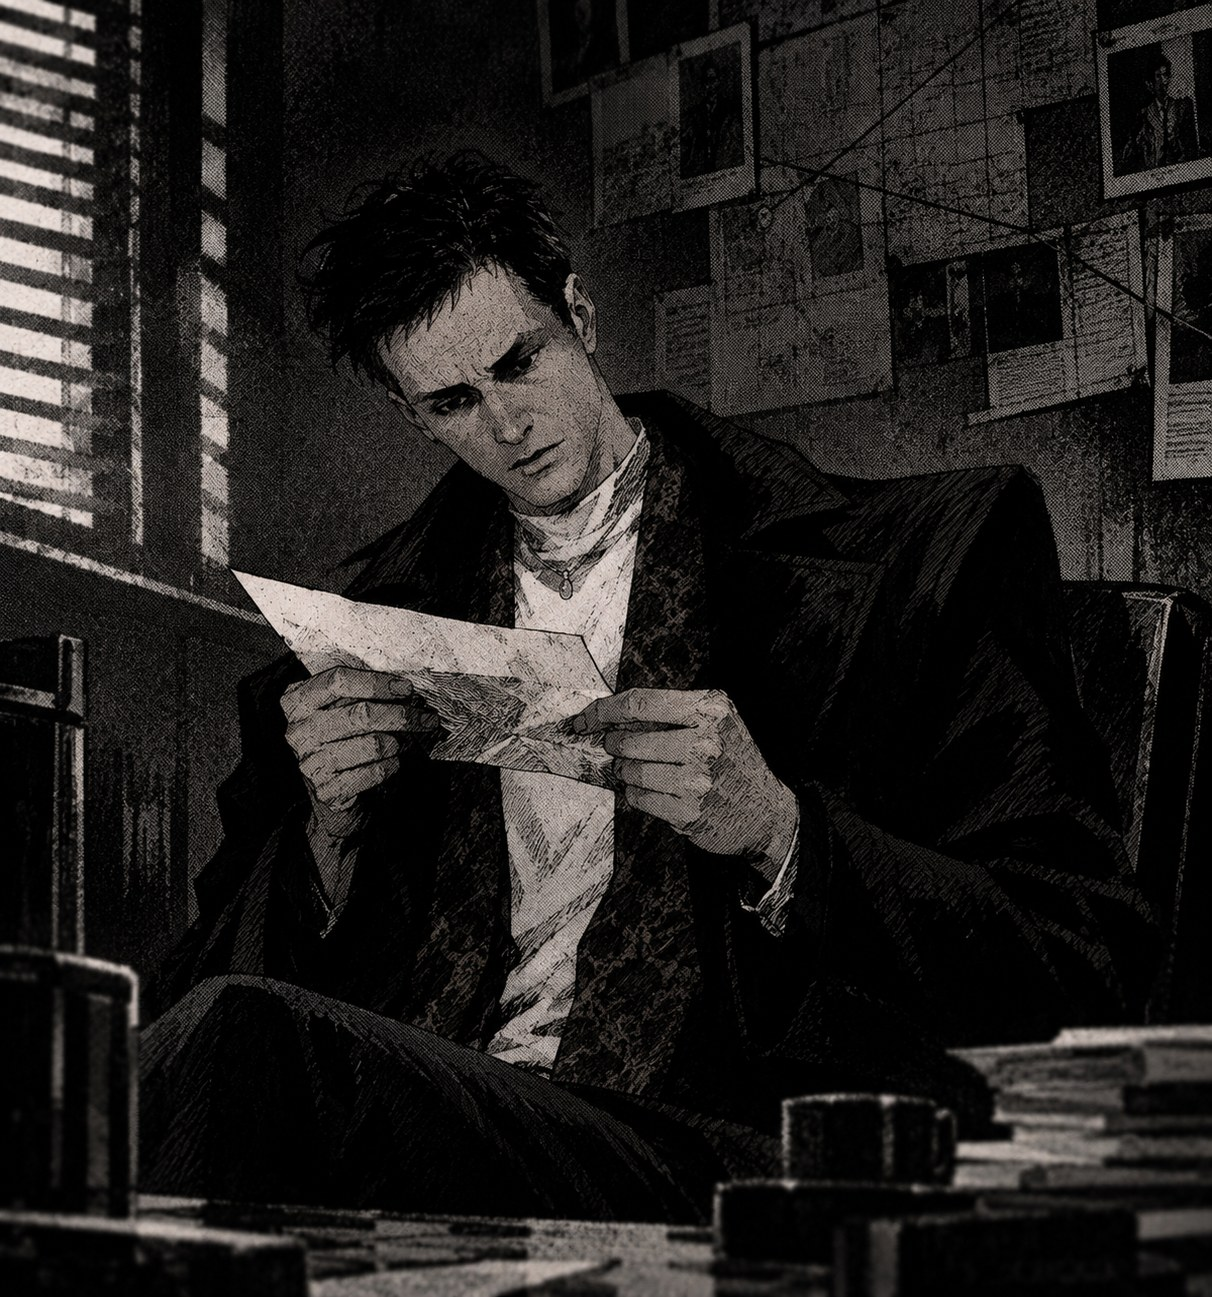
\includegraphics[width=0.66\linewidth]{cover.jpg}}}\par}
\vspace{7mm}
{\disp\blackface\fontsize{20}{22}\selectfont\addfontfeature{LetterSpace=30}ALEX MERSER\par}
\vspace{3mm}
{\disp\fontsize{8.4}{10}\selectfont\addfontfeature{LetterSpace=32}\textcolor{accent}{АЛЕКС МЕРСЕР}\par}
\vfill
{\disp\fontsize{8}{11.5}\selectfont По мотивам семинаров Альфреда Коржибски\\по общей семантике\par}
\vspace{2.5mm}
{\disp\fontsize{7.6}{9}\selectfont\addfontfeature{LetterSpace=30}\textcolor{accent}{КОЛЛЕДЖ ОЛИВЕТ · 1937}\par}
\vspace{5mm}
\end{center}
\clearpage
\nopagecolor\color{black}\restoregeometry

% --- страница серии (в стиле «Вирусо-логии семантических-реакций»)
\thispagestyle{empty}
\vspace*{0.455\textheight}
\begin{center}
{\large\bfseries ОБЩАЯ-СЕМАНТИКА\par}
\vspace{2.2mm}
{\itshape\addfontfeature{LetterSpace=12}НАУКА ЧЕЛОВЕЧЕСКИХ ОЦЕНОК\par}
\end{center}
\clearpage
% --- издательский титул
\thispagestyle{empty}
\vspace*{0.40\textheight}
\begin{center}
{\large Карта не есть территория.\\[1.2ex]
Научно-нуарный детектив по мотивам семинаров\\Альфреда Коржибски, Оливет, 1937.,\par}
\vfill

\includegraphics[width=17mm]{logo.png}\par
\vspace{3.5mm}
{SocioCyberneering Inc.\par}
\vspace{2.5mm}
{19 ноября 2026 г.\par}
\vspace{6mm}
\end{center}
\clearpage
\thispagestyle{empty}
\begin{center}
\vspace*{0.13\textheight}
{\disp\fontsize{8}{10}\selectfont\addfontfeature{LetterSpace=45}НАУЧНО-НУАРНЫЙ ДЕТЕКТИВ\par}
\vspace{9mm}
{\disp\blackface\fontsize{25}{28}\selectfont Карта не есть территория\par}
\vspace{5mm}
{\color{accent}\rule{0.36\linewidth}{0.6pt}}\par
\vspace{7mm}
{\disp\fontsize{15}{18}\selectfont\addfontfeature{LetterSpace=24}ALEX MERSER\par}
\vspace{2mm}
{\disp\fontsize{8.5}{10}\selectfont\addfontfeature{LetterSpace=24}\textcolor{accent}{АЛЕКС МЕРСЕР}\par}
\vspace{10mm}
{\itshape Детектив по мотивам семинаров Альфреда Коржибски\\по общей семантике в колледже Оливет, 1937 год\par}
\vfill
{\footnotesize Художественная история. Детектив, преступление и диалоги вымышлены; идеи Коржибски служат интеллектуальной основой сюжета.\par}
\vspace{6mm}
\end{center}
\clearpage
\clearpage\thispagestyle{empty}
\begin{center}\vspace*{\fill}
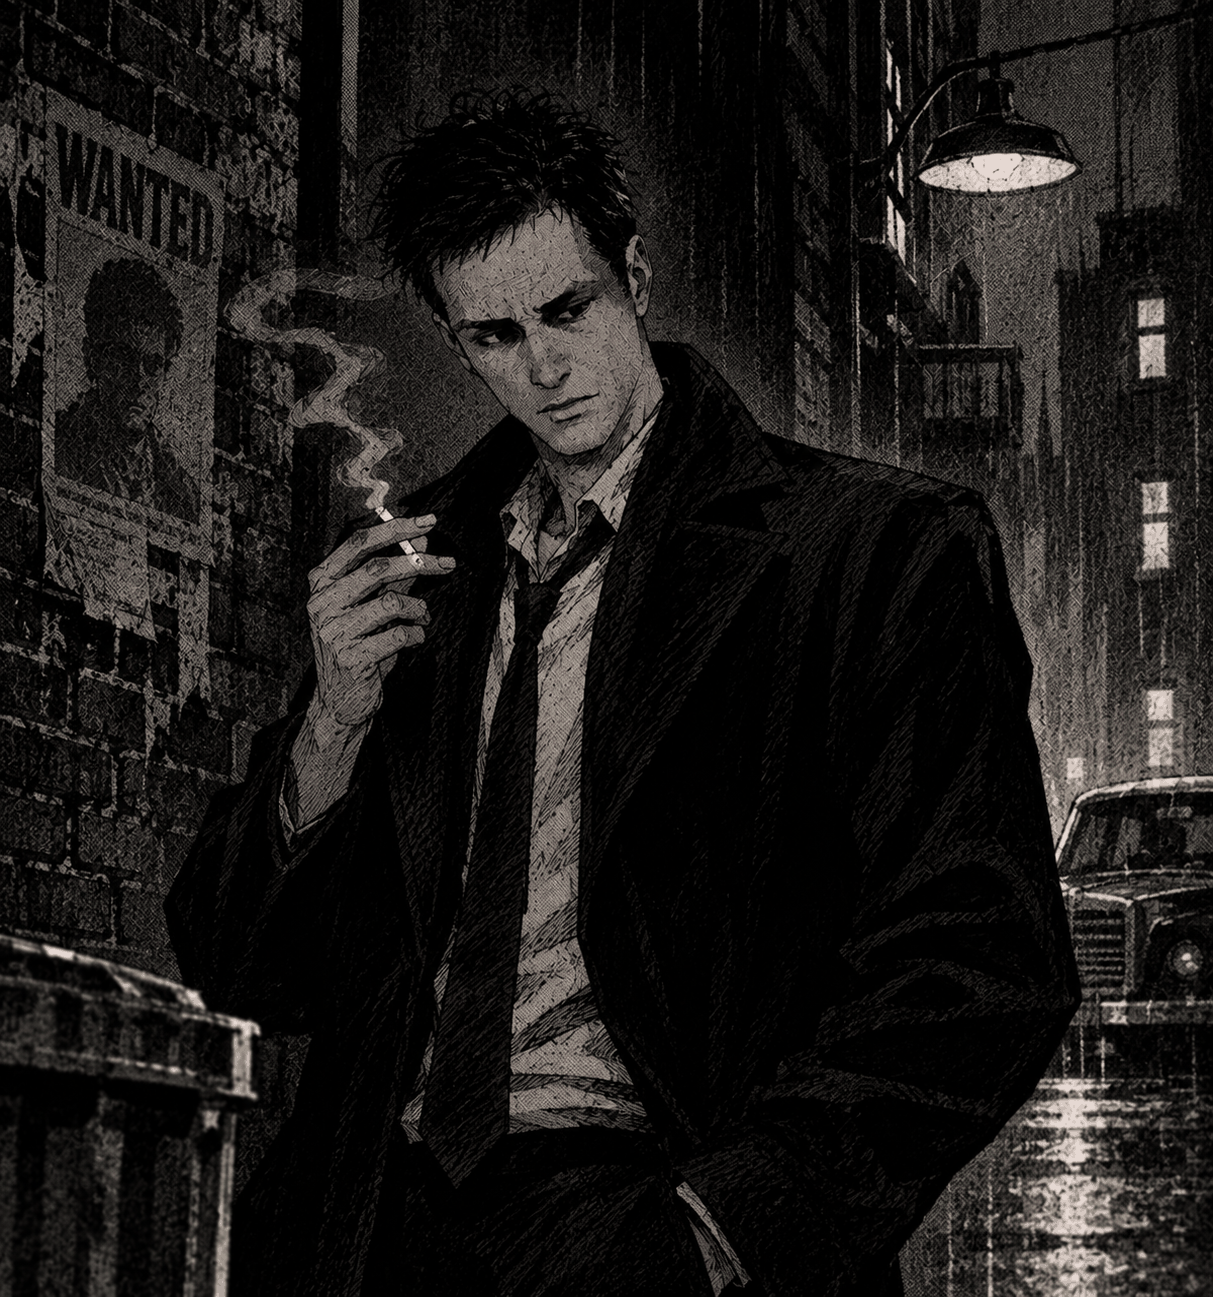
\includegraphics[width=0.94\textwidth,height=0.80\textheight,keepaspectratio]{img/p_mercer.png}\par
\vspace{4mm}
{\disp\fontsize{8}{10}\selectfont\addfontfeature{LetterSpace=30}АЛЕКС МЕРСЕР\par}
\vspace{1.5mm}
{\footnotesize\itshape В документах --- Джулиан Александр Мерсер, отсюда «J.~M.» на всех бумагах.\par}
\vspace*{\fill}\end{center}\clearpage

\clearpage\thispagestyle{empty}
\begin{center}
{\disp\fontsize{7.6}{9}\selectfont\addfontfeature{LetterSpace=40}\textcolor{accent}{СТРАНИЦА, КОТОРУЮ ОБЫЧНО НЕ ЧИТАЮТ}\par}
\vspace{3mm}
{\disp\bfseries\fontsize{15}{18}\selectfont Права, которые мы\\не стали защищать\par}
\vspace{2.5mm}
{\color{accent}\rule{17mm}{0.6pt}}\par
\end{center}
\vspace{3mm}
\begin{notebox}{Как обычно пишут на этом месте}
\small\itshape Все права защищены. Никакая часть настоящего издания не может быть воспроизведена, записана, перепечатана, пересказана вслух, пересказана шёпотом, процитирована за ужином, выучена наизусть, увидена во сне или помыслена без предварительного письменного разрешения правообладателя. Нарушители будут преследоваться по закону, а также взглядом.
\end{notebox}

\noindent Мы прочитали это вслух и услышали, как бирка ест территорию. Книга про то, что карта не есть территория, не может начинаться с обещания посадить вас за пересказ карты.

\medskip\noindent Поэтому по-человечески.

\vspace{1mm}
\medskip\noindent\textbf{Эта книга открыта.} Лицензия CC~BY-SA~4.0. Это значит:

\begin{itemize}\setlength{\itemsep}{0pt}
\item копируйте;
\item печатайте --- дома, в типографии, на работе, пока начальник не видит;
\item раздавайте бесплатно и дарите;
\item режьте на цитаты;
\item переводите на любой язык, включая те, на которых ещё не говорят;
\item читайте вслух, шёпотом и во сне --- отдельное разрешение на сон прилагается;
\item переделывайте, спорьте, дописывайте главы, которых здесь не хватает.
\end{itemize}

\medskip\noindent Три просьбы. Это и есть вся лицензия; остальное --- её перевод на юридический.

\begin{enumerate}\setlength{\itemsep}{1pt}
\item \textbf{Скажите, откуда взяли.} В лицензии это буквы BY: укажите авторство.
\item \textbf{Оставьте дальше открытым.} То, что выросло из открытого, закрытым не становится. В лицензии это буквы SA.
\item \textbf{Не выдавайте карту за территорию.} Изменили текст --- напишите, что изменили. Иначе читатель будет судить автора по вашей правке, а это уже не лицензия, это подлог.
\end{enumerate}

\medskip\noindent Исходники --- файлы вёрстки «.tex», схемы, весь набор --- на тех же правах. Если вам привычнее GPL, считайте, что у схем GPL: берите, меняйте, но передавайте вместе с исходником и не закрывайте. Разница между CC~BY-SA и GPL здесь ровно одна: первая написана для текстов, вторая --- для кода, а смысл у обеих общий и умещается в четыре слова: \textit{открытое остаётся открытым}.

\medskip
\noindent\textbf{Где лежат исходники.} Весь набор --- текст, схемы, файлы вёрстки --- здесь:

\begin{center}
\href{https://github.com/sociocyber1/Latex_ScienceBook_Detective-Alex-Merser-Map-is-not-Territory}%
{\resizebox{0.99\linewidth}{!}{github.com/sociocyber1/Latex\_ScienceBook\_Detective-Alex-Merser-Map-is-not-Territory}}
\end{center}

\noindent Скачивайте, собирайте у себя, исправляйте опечатки, присылайте правки, делайте свою версию.

\vspace{1mm}
\medskip\noindent\textbf{Чего всё-таки нельзя.} Нельзя закрыть то, что открыли (единственная оговорка --- на следующей странице). Нельзя подписать своим именем чужое. Нельзя продавать как «эксклюзивное издание»: эксклюзива нет, книга лежит в сети, бесплатно, и завтра будет лежать там же.

\vspace{1mm}
\medskip\noindent\textbf{Санкции.} За нарушение этой лицензии не предусмотрено ни штрафа, ни суда, ни коллекторов, ни взгляда. Предусмотрено только то, что вы будете человеком, который закрыл открытое. Это дороже.

\clearpage
\thispagestyle{empty}
\begin{center}
{\disp\fontsize{7.6}{9}\selectfont\addfontfeature{LetterSpace=40}\textcolor{accent}{ПРОДОЛЖЕНИЕ ТОЙ ЖЕ СТРАНИЦЫ}\par}
\vspace{3mm}
{\disp\bfseries\fontsize{13.5}{17}\selectfont Печатать, продавать\\и поддержать\par}
\vspace{2.5mm}
{\color{accent}\rule{17mm}{0.6pt}}\par
\end{center}
\vspace{2mm}

\noindent\textbf{Хотите печатать и продавать --- печатайте и продавайте.} Запрета нет, разрешения спрашивать не надо, процент автору платить не надо. Книга для того и открыта.

\noindent Три условия, и ни одно из них не про деньги:

\begin{enumerate}\setlength{\itemsep}{1pt}
\item \textbf{оставьте ссылку на оригинал} --- адрес исходников с предыдущей страницы;
\item \textbf{оставьте имя автора} и название --- не ради тщеславия, а чтобы читателю было с чем сравнить;
\item \textbf{приложите список изменений:} что сократили, что добавили, что исправили. Хоть одной страницей в конце. Это главное из трёх: без него ваш читатель будет судить об авторе по вашей правке и даже не узнает об этом.
\end{enumerate}

\medskip\noindent\textbf{Не закрывайте книгу.} Переиздание остаётся открытым --- это условие лицензии, а не пожелание.

Но бывает всякое. Если издательство требует закрытой лицензии и иначе не берёт --- берите и печатайте закрытым, пусть книга дойдёт до людей. Только сделайте одну вещь: \textbf{поставьте сноску на оригинал} и напишите прямо, что существует открытая версия, вот по этому адресу, бесплатно. Чтобы читатель знал, что у него есть выбор.

\noindent Закрытая книга, которая честно говорит, где лежит открытая, --- приемлемо. Закрытая книга, которая об этом молчит, --- нет.

\bigskip
\begin{center}{\disp\bfseries\fontsize{11}{14}\selectfont Поддержать автора и выход новых материалов\par}\end{center}

\noindent Если вы считаете эту работу полезной --- можно помочь деньгами. Коротко, без драматургии: автор делает всё сам, из своего кармана и бесплатно, а подписки, инструменты и время на них расходуются вполне материально.

\begin{center}
\fbox{\parbox{0.72\linewidth}{\centering\textbf{Сбер}\\[1.2mm]
{\disp\fontsize{12.5}{15}\selectfont\addfontfeature{LetterSpace=8}2202\hspace{2mm}2050\hspace{2mm}2451\hspace{2mm}1591}}}
\end{center}

\begin{notebox}{На полях, рукой Мерсера}
\small Автор раздал книгу даром, а страницей позже просит денег. Противоречие я отметил сразу и вслух.

Он ответил: «одно другому не мешает». Я проверил --- не мешает. В заложниках книга не сидит: не заплатите --- получите ровно то же самое, целиком, без сокращений, без «расширенной версии для поддержавших» и без вырезанной главы. Лимита на читателя нет.

Это называется просьбой, а не ценой, и разница та же, что между картой и территорией: выглядит похоже, работает совсем иначе.

Так что подавайте, если считаете нужным. Посмеяться я всё равно успел.

\textit{P.~S. Номер в рамке автор дописал последним, уже после того, как написал про деньги целую страницу и забыл указать, куда их слать. Я сверил: шестнадцать цифр, четыре группы по четыре, больше о нём сказать нечего. И отдельно, по привычке: это карта карты. Цифры --- не деньги, деньги --- не благодарность, благодарность --- не обязанность. Четыре разных уровня, и путать их не нужно ни автору, ни вам.}
\end{notebox}

\vspace{3mm}
\begin{center}
{\disp\fontsize{9}{12}\selectfont\addfontfeature{LetterSpace=16}SocioCyberneering Inc.\par}
\vspace{1.5mm}
{\itshape\small Все права розданы.\par}
\vspace{2mm}
{\footnotesize Связь с автором --- на странице «Благодарности» в конце книги.\par}
\end{center}
\clearpage

\thispagestyle{empty}
\vspace*{0.26\textheight}
\begin{center}
{\disp\blackface\fontsize{17}{22}\selectfont\addfontfeature{LetterSpace=8}ВЕДЁМ РЕВОЛЮЦИЮ\\В ОЦЕНКЕ\par}
\vspace{9mm}
{\color{accent}\rule{24mm}{0.6pt}}\par
\vspace{9mm}
{\disp\blackface\fontsize{17}{22}\selectfont\addfontfeature{LetterSpace=8}КОНЕЦ ВОЙНЕ\par}
\vspace{9mm}
{\color{accent}\rule{24mm}{0.6pt}}\par
\vspace{9mm}
{\disp\blackface\fontsize{17}{22}\selectfont\addfontfeature{LetterSpace=8}ОТКРОЙ ЧЁРТОВ РАЗУМ\par}
\vfill
{\itshape\small Первый лозунг --- из тысяча девятьсот тридцать седьмого.\\
Второй --- оттуда же, и он до сих пор не выполнен.\\
Третий --- от автора, которому надоело просить вежливо.\par}
\vspace{10mm}
\end{center}
\clearpage
\tableofcontents

\storypartT{Предисловие: о чём эта книга и зачем она}

\noindent Это детектив. Тысяча девятьсот тридцать седьмой год, маленький американский колледж, два трупа с разницей в год, сыщик по имени Алекс Мерсер и человек, который полгода считал виновным не того.

И это учебник. Только вместо параграфов --- дело, вместо контрольных --- ошибки Мерсера, а вместо преподавателя с указкой --- польский инженер Альфред Коржибски, который летом тридцать седьмого действительно читал в колледже Оливет семинар по общей семантике.

\medskip\noindent\textbf{Общая семантика --- это про то, как мы оцениваем.} Не про слова, хотя начинается со слов. Про зазор между тем, что есть, и тем, что мы об этом сказали. Между событием и фамилией. Между человеком и биркой, которую мы на него повесили, --- «убийца», «дурак», «враг», «наш».

Главная фраза Коржибски вынесена на обложку: \textit{карта не есть территория}. У неё есть продолжение, которое цитируют реже: карта покрывает не всю территорию, и хорошая карта похожа на территорию \textit{структурой}. Три строки. Из них растёт всё остальное: даты, индексы, кавычки, «и так далее», структурный дифференциал, отложенная реакция.

\medskip\noindent\textbf{Почему детектив.} Потому что сыщик --- это человек, чья профессия целиком состоит из оценки. Он смотрит на факты и говорит, что они значат. И он единственный, у кого цена ошибки видна сразу: не «неточная формулировка», а живой человек в камере. Когда Шерлок Холмс с одного взгляда называет вам профессию, биографию и мотив, это красиво. Когда так делает настоящий следователь, это называется иначе.

Мерсер начинает книгу именно таким. Он уверен, он быстр, он уже знает, кто виноват. Дальше ему придётся разбирать собственную уверенность на части --- по одной.

\medskip\noindent\textbf{Зачем это вам, если вы не сыщик.} Затем, что вы оцениваете каждый день, только без протокола. Начальник «придирается». Сосед «хамит». Страна «агрессивная». Врач «ничего не понимает». Каждая из этих фраз --- готовый приговор, вынесенный за полсекунды, и почти всегда по одному наблюдению, в котором участвовали освещение, усталость, чужой пересказ и ваше настроение.

Коржибски писал всё это после войны, на которой был. Он считал --- всерьёз, не как метафору, --- что люди убивают друг друга в том числе потому, что путают бирку с человеком, слово с вещью, год прошлый с годом нынешним. Отсюда и три лозунга на предыдущей странице. Они звучат громко. Они и задуманы громкими.

\medskip\noindent\textbf{Как читать.} В книге три вида глав, и вы вправе обращаться с ними как угодно.

\begin{itemize}\setlength{\itemsep}{1pt}
\item \textbf{Части} --- само дело. Если вам нужен только детектив, читайте одни их: история связная, без пропусков.
\item \textbf{Интермедии} --- остановки. Здесь Мерсер разбирает, что он только что сделал неправильно, и на чём именно сломалась его голова. Это та же история, только изнутри метода.
\item \textbf{Семинар} --- четырнадцать лекций, голосом Коржибски. Их можно читать подряд, отдельно от сюжета, как короткий курс. Порядок в них выстроен от простого к сложному.
\end{itemize}

Сквозной порядок --- рекомендованный: приём появляется в интермедии только после того, как его объяснили на семинаре, и только после того, как Мерсер на нём обжёгся.

\medskip\noindent\textbf{Честные оговорки, без которых книга была бы ровно тем, против чего написана.}

\begin{enumerate}\setlength{\itemsep}{1pt}
\item Коржибски --- реальный человек. Его биография и его идеи взяты из источников. Его \textit{реплики} в этой книге написаны автором. Это литературный персонаж, а не стенограмма.
\item Дело, колледж, убитые, свидетели, документы --- вымышлены целиком. Совпадения с настоящими делами не предполагались.
\item Факты из будущего (а такие в книге есть) проверялись. Как именно --- показано внутри, в одной из интермедий, вместе с тем, что проверку не прошло. Это не кокетство: книга про проверку обязана показать свою.
\item Четвёртая стена здесь регулярно ломается, и автор время от времени получает от собственного героя. Это сделано нарочно и ровно по третьему положению общей семантики, которое разрешает говорить о говорении.
\end{enumerate}

\medskip\noindent\textbf{Чего эта книга не делает.} Она не обещает, что вы перестанете ошибаться. Коржибски такого не обещал, а он был смелее. Она предлагает другое: заметить зазор. Между тем, что случилось, и тем, что вы об этом сказали. Между человеком и фамилией. Между картой и территорией.

Дальше зазор никуда не денется. Но в него можно перестать проваливаться каждый раз.

\vspace{2mm}
\medskip\noindent И последнее. Эта книга --- тоже карта. Со своими пробелами, своим масштабом и своей датой на обложке.

\begin{center}\itshape Проверяйте.\end{center}
\clearpage
\mainmatter

% ------------------------------------------------ source lines 51-696
\storypartL{Часть I}
\storysection{Пролог}{Оливет, Мичиган}
\textbf{Конец февраля 1937 года.}

Дождь барабанил по окнам колледжа.

В Америке всё ещё помнили Великую депрессию. Люди теряли работу, банки теряли деньги, а политики находили виноватых.

У каждого была своя теория.

Коммунисты обвиняли капиталистов. Капиталисты обвиняли коммунистов. Священники обвиняли грешников. Грешники обвиняли Бога.

Все знали, кто виноват.

Никто не знал, что делать.

Меня звали Алекс Мерсер. По документам — Джулиан Александр: мать выбрала два имени, а ребёнок был один. Отсюда «J. M.» на бумагах и «Алекс» для всех остальных. Тридцать два года. Бывший газетный репортёр. Бывший полицейский. Человек, который слишком долго смотрел на человеческие пороки и в конце концов начал путать их со всем человечеством.

Я приехал в Оливет по делу об убийстве.

Погиб студент.

Его звали Томас Рид.

Его нашли в комнате общежития накануне вечером. Один выстрел в грудь. Запертая дверь. Исчезнувшая записная книжка.

Полиция уже нашла подозреваемого.

Эдвард Миллер.

Сосед погибшего. Политический радикал. Человек с дурной репутацией и ещё худшими знакомыми.

У полиции было всё, что требовалось для обвинения.

Мотив.

Возможность.

И свидетель, утверждавший, что видел Миллера возле комнаты убитого.

Дело выглядело простым.

А простые дела, как правило, заканчиваются тем, что кто-нибудь невиновный отправляется на электрический стул.

Я вошёл в аудиторию.

У доски стоял невысокий человек с густыми усами.

Альфред Коржибски.

Он собирался читать лекцию о человеческом мышлении.

Я собирался выяснить, кто убил студента.

Тогда я ещё не знал, что это одно и то же дело.

\gap{0}
\clearpage
\storysection{Глава I}{Слово «убийца»}
Коржибски говорил спокойно.

Он не пытался выглядеть пророком. Не обещал избавить человечество от невежества. Не предлагал новую веру.

Он задавал вопросы.

— Когда вы говорите, что знаете человека, что именно вы знаете?

Кто-то из студентов ответил:

— Его характер.

— Что вы называете характером?

Студент замялся.

Коржибски подождал.

— Его поведение, — наконец ответил тот.

— Какое именно?

В аудитории стало тихо.

Я достал записную книжку.

Мне нравились люди, которые задавали вопросы. Обычно они меньше говорили глупостей.

— Предположим, — продолжил Коржибски, — человек однажды совершил поступок, который вы считаете плохим. Вы называете его плохим человеком. Но описывает ли это слово всё, что он делал, делает и может сделать?

— Нет, — ответил студент.

— Тогда почему вы используете его так, будто оно описывает всё?

Я посмотрел на собственные записи.

В полицейском отчёте Миллер значился как «опасный агитатор».

Я сам повторил это выражение трижды за утро.

Опасный агитатор.

Два слова.

И ни одного конкретного факта о том, где он находился в момент убийства.

Я закрыл блокнот.

Впервые за долгое время мне стало не по себе от собственного языка.

\gap{1}
\clearpage
\storysection{Глава II}{Четырнадцать лекций и одна смерть}
После занятия я дождался Коржибски в коридоре.

— Профессор, мне нужно поговорить с вами.

— Конечно.

Я рассказал ему об убийстве.

Он выслушал меня, не перебивая.

— Полиция считает Миллера убийцей, — закончил я. — Но доказательства косвенные.

— Тогда вы ещё не знаете, кто убийца.

— Я знаю, что полиция считает его убийцей.

— Это другое утверждение.

Я раздражённо выдохнул.

— Вы всегда так разговариваете?

— Как?

— Разбираете каждое слово на части.

Он улыбнулся.

— Нет. Иногда я разбираю целые предложения.

Я не улыбнулся.

— Человек мёртв, профессор.

— Да. Это событие. Ваше описание события — не само событие. Если вы хотите установить, что произошло, вам следует различать их.

Я посмотрел на него.

— И как мне это сделать?

— Начните с наблюдений. Не с выводов.

Он взял лист бумаги и провёл горизонтальную линию.

— Представьте, что вы смотрите на происходящее. Ваша нервная система отбирает информацию. Затем вы организуете её, интерпретируете, называете. На каждом этапе что-то может быть упущено.

Он написал на листе:

\textbf{СОБЫТИЕ  $\to$  НАБЛЮДЕНИЕ  $\to$  ОПИСАНИЕ  $\to$  ВЫВОД}

— Вы не получаете всю реальность, мистер Мерсер. Вы получаете ограниченную информацию о ней. Поэтому необходимо помнить, что вы абстрагируете.

Я посмотрел на схему.

— Значит, свидетель мог ошибиться?

— Конечно.

— Полиция могла ошибиться?

— Разумеется.

— А вы?

Коржибски посмотрел мне прямо в глаза.

— Особенно я.

Впервые за день я почувствовал, что нахожусь рядом с человеком, который не пытался продать мне собственную непогрешимость.

Я вернулся в полицейский участок.

И перечитал показания свидетеля.

\gap{2}
\clearpage
\storysection{Глава III}{Человек, который видел слишком много}
Свидетеля звали Уильям Кларк.

Двадцать лет. Студент. Сын уважаемого местного врача.

Он утверждал, что видел Миллера возле комнаты Рида примерно в девять вечера.

— Вы уверены, что это был Миллер? — спросил я.

— Да.

— Как далеко вы находились?

— Через весь коридор.

— Какое там было освещение?

— Обычное.

— Что значит «обычное»?

Он посмотрел на меня с раздражением.

— Вы хотите сказать, что я лгу?

— Нет. Я хочу узнать, что именно вы видели.

Кларк сжал губы.

— Я видел человека, похожего на Миллера.

— Похожего?

— Да.

— А в первоначальном показании вы написали, что видели Миллера.

Он замолчал.

Я положил перед ним лист бумаги.

— Опишите его одежду.

Кларк назвал тёмное пальто.

— Головной убор?

Он задумался.

— Не помню.

— Рост?

— Примерно как у Миллера.

— Лицо?

— Я не разглядел.

Я откинулся на спинку стула.

Свидетель не обязательно лгал.

Он мог действительно видеть человека в коридоре.

Но затем его память, ожидания и последующие разговоры могли превратить неопределённый силуэт в конкретного человека.

Сначала он увидел фигуру.

Потом решил, что это Миллер.

Потом начал вспоминать, будто с самого начала был уверен.

Я не мог утверждать, что именно так всё и произошло. Для этого требовались дополнительные сведения.

Но теперь у нас был вопрос, который следовало проверить.

Кто ещё мог находиться в коридоре?

И почему Кларк так быстро согласился с версией полиции?

\gap{3}
\clearpage
\storysection{Глава IV}{Индекс, которого не было}
Я вернулся в комнату погибшего.

На письменном столе лежали учебники, газетные вырезки и пачка писем.

В одном письме Рид упоминал, что собирается опубликовать материалы о финансовых махинациях в студенческом фонде.

Я перечитал письмо.

Томас подозревал, что кто-то подделывал бухгалтерские записи.

Возможно, это и было причиной убийства.

Но имя подозреваемого в письме отсутствовало.

На полях Рид написал:

«Кларк знает больше, чем говорит».

Я почувствовал, как внутри что-то сдвинулось.

Уильям Кларк.

Тот самый свидетель.

Я начал проверять даты.

Сначала нашёл запись о собрании студенческого комитета.

Затем расписание занятий.

Потом список людей, имевших доступ к бухгалтерским документам.

Кларк входил в комитет.

Именно он отвечал за часть финансовой отчётности.

У меня появился мотив для дальнейшего расследования.

Но мотив не был доказательством убийства.

Я записал это большими буквами.

\textbf{МОТИВ ≠ ДОКАЗАТЕЛЬСТВО.}

Я почти рассмеялся.

Коржибски начинал действовать мне на нервы.

Теперь даже мои собственные мысли требовали оформления.

Но я продолжил проверку.

В документах обнаружилась странность: сумма, которую Рид собирался проверить, исчезла из отчёта за несколько недель до убийства.

Кто-то изменил цифры.

Кто-то хотел, чтобы это осталось незамеченным.

И кто-то очень торопился закрыть дело.

\gap{4}
\clearpage
\storysection{Глава V}{Дата и индекс}
На следующий день я снова встретил Коржибски.

Он пил кофе в маленькой комнате возле аудитории.

Я положил перед ним свои записи.

— Я думаю, что свидетель причастен к делу.

— На каком основании?

Я объяснил.

Коржибски прочитал листы.

— Это интересная гипотеза.

— Вы мне не верите?

— Я не обязан выбирать между верой в вас и неверием в вас. Я могу изучить ваши основания.

Он вернул записи.

— Не превращайте человека в неизменную категорию. И не забывайте, что один человек в разные моменты времени не во всех отношениях одинаков.

Я вспомнил, что читал о его подходе к языку.

Чтобы не смешивать разные случаи и состояния, полезно использовать индексы и даты.

Вместо «Кларк лжец» — «Кларк в показании от такого-то числа сообщил, что видел Миллера, но при повторном опросе признал, что не разглядел лицо».

Это было длиннее.

Зато честнее.

Я переписал свои записи.

Затем проверил алиби Кларка.

В девять вечера он якобы находился в библиотеке.

Но библиотекарь вспомнил, что Кларк ушёл раньше.

Время его ухода никто точно не записал.

Убийство произошло в промежутке, когда его местонахождение не было подтверждено.

Это ещё ничего не доказывало.

Но теперь у меня были основания допросить его повторно.

\gap{5}
\clearpage
\storysection{Глава VI}{Человек в зеркале}
Кларк согласился встретиться со мной вечером.

Он пришёл в маленькое кафе возле колледжа.

Снаружи шёл дождь.

— Вы думаете, это я убил Рида? — спросил он.

— Я думаю, что вы скрываете информацию.

— Это не одно и то же.

Я посмотрел на него.

Он усмехнулся.

— Вы разговаривали с профессором Коржибски.

Я ничего не ответил.

— Он учит вас сомневаться во всём?

— Нет. Он учит меня различать то, что я наблюдаю, и то, что заключаю из наблюдений.

Кларк посмотрел в окно.

— А если вы никогда не сможете узнать правду?

— Тогда я буду знать меньше, чем мне хотелось бы.

— И вас это устроит?

— Нет.

Я наклонился вперёд.

— Но я не собираюсь заменять отсутствие доказательств красивой историей.

Его лицо изменилось.

На несколько секунд я увидел не подозреваемого, не студента и не финансового секретаря.

Я увидел испуганного человека.

— Рид собирался уничтожить мою жизнь, — сказал он.

— Почему?

— Он узнал о деньгах.

— Вы присвоили их?

Кларк молчал.

— Сколько?

— Я не помню точно.

— Тогда найдём документы.

Он резко поднял голову.

— Вы не понимаете! Если это выйдет наружу, отец меня уничтожит. Все будут знать, что я сделал.

— Что именно вы сделали?

Он встал.

— Я не убивал его!

— Я этого не утверждал.

Кларк замер.

Я действительно не утверждал.

И впервые он понял, что его слова не могут заставить меня принять его вину или невиновность заранее.

Он сел обратно.

— Я подделывал отчёты, — сказал он. — Но в ту ночь я не был в комнате Рида.

— Где вы были?

— У себя. Один.

— Это не алиби.

— Я знаю.

Он опустил голову.

— Но я видел человека, который вошёл в общежитие.

— Кого?

— Не знаю. Я видел его со спины.

— Почему вы не сказали об этом полиции?

Кларк посмотрел на меня.

— Потому что я боялся, что они начнут задавать вопросы о деньгах.

Теперь у меня было новое направление расследования.

Не ответ.

Направление.

Иногда это единственное, что может дать тебе ночь, проведённая рядом с человеческой ложью.

\gap{6}
\clearpage
\storysection{Глава VII}{Неаристотелевская ночь}
Я вернулся в общежитие и снова осмотрел коридор.

На этот раз я не искал Миллера.

Я искал человека.

Не конкретного человека. Не готовую категорию.

Человека, который мог войти в здание, пройти к комнате Рида и выйти, не привлекая внимания.

Я изучил расположение дверей.

Расписание дежурств.

Сведения о ключах.

Список сотрудников, имевших доступ к зданию.

Я проверил каждый пункт отдельно.

И обнаружил, что у заведующего хозяйством был запасной ключ.

Его звали Гарольд Беннет.

Он также подписывал документы студенческого фонда.

Именно его подпись стояла возле исправлений в бухгалтерских книгах.

Я нашёл его в кабинете поздно вечером.

— Вы знали Рида? — спросил я.

— Конечно. Все его знали.

— Он проверял бухгалтерские документы.

— И что?

— Вы подписывали исправления.

Беннет усмехнулся.

— Я подписываю сотни документов.

— А запасной ключ?

Улыбка исчезла.

— Что с ним?

— Где он был в ночь убийства?

— На месте.

— Кто-нибудь ещё мог его взять?

— Не знаю.

Он отвечал слишком быстро.

Но даже теперь я не мог назвать его убийцей.

Я мог только продолжать проверку.

В кабинете я заметил бумажную папку с вырванными страницами.

На одной из оставшихся страниц была сумма, совпадавшая с исчезнувшими деньгами.

А рядом — подпись Кларка.

Всё оказалось сложнее, чем я предполагал.

Кларк действительно подделывал отчёты.

Беннет действительно участвовал в оформлении документов.

Но кто из них убил Рида?

И убил ли его кто-то из них вообще?

Я посмотрел на часы.

До рассвета оставалось несколько часов.

Я чувствовал усталость.

Но теперь у меня была хотя бы одна вещь, которой не было в начале расследования.

Не уверенность.

Метод.

\gap{7}
\clearpage
\storysection{Глава VIII}{Территория}
На следующее утро я снова пришёл на лекцию.

Коржибски стоял перед аудиторией.

— Мы часто реагируем не только на то, что происходит, но и на то, что это для нас означает, — говорил он. — Слова могут вызывать реакции, которые мы принимаем за свойства самих вещей.

Я сел в последнем ряду.

Вчера слово «убийца» означало для меня Миллера.

Сегодня я знал, что это было лишь название, которое полиция прикрепила к подозреваемому.

Я ещё не знал, кто убил Рида.

Я не знал, солгал ли Кларк о человеке, которого видел.

Я не знал, какую роль сыграл Беннет.

Но я знал, что каждый из этих вопросов требовал отдельного ответа.

И что ни один ответ нельзя было получить простым повторением чужой уверенности.

После лекции я вышел на улицу.

Дождь прекратился.

Город выглядел почти мирным.

Но я больше не доверял этому впечатлению.

Мир не обязан соответствовать тому, как он выглядит с первого взгляда.

Люди не обязаны соответствовать названиям, которые мы им даём.

И даже самая убедительная история может оказаться ложной.

Я достал блокнот и записал:

«Дело Рида. Продолжить расследование. Проверить ключи, бухгалтерские документы, показания Кларка. Не путать подозрение с доказательством».

Затем добавил:

«Не путать собственную уверенность с истиной».

Я закрыл блокнот.

Впервые за долгое время я не чувствовал необходимости немедленно вынести приговор.

Впереди была работа.

И, возможно, именно с этого начиналось настоящее мышление.

\textbf{Карта не есть территория.}

Но карта, которую постоянно сверяют с территорией, всё ещё может помочь найти дорогу.


% ------------------------------------------------ INTERLUDE 1 (after Часть I)
\storypart{Интермедия 1}{Дождь по расписанию}{Интермедия 1. Дождь по расписанию}
\dateline{Оливет, Мичиган. Утро. Яркое.}
\pageimg{img/c_rain.png}{Интермедия первая, как её увидел художник: солнце, снеговик и сыщик, которому обещали дождь}
Я проснулся от птиц.

Первым делом я проверил окно. Это профессиональное: нуарное утро начинается с погоды, как суд начинается со слов «встать, суд идёт». Погода была, но не та. Над общежитием висело солнце — круглое, жёлтое, довольное собой, как цыплёнок на открытке. Снег сиял так, словно его вычистили зубным порошком.

— Нет, — сказал я вслух. — Так не пойдёт.

Я знаю правила. Нуар обязан быть мокрым. Дождь — это не осадки, это контракт. Читатель берёт книгу, потому что ему обещали мрак, блики фонарей на мостовой и мужчину в плаще, который смотрит на лужу так, будто она ему должна денег. А мне предложили газон. Заснеженный, но всё равно газон. На нём стоял снеговик с морковью вместо носа и выражением лица, подозрительно счастливым для свидетеля убийства.

Я надел плащ. Плащ был сух, как налоговая декларация.

В дверях меня встретил доктор Хейл. Он улыбался. Это уже было уликой.

— Доброе утро, Мерсер!

— Вы улыбаетесь. Нашлось ещё одно тело?

— Нашлись тёплые носки. Жена связала.

Он выставил ногу. Носок был зелёный, с оленем. Я смотрел на оленя долго, как смотрят на показания, которым не доверяют.

— Доктор, в такую погоду нельзя расследовать убийство. Нет атмосферы.

— У убийцы тоже нет расписания, Мерсер. Он не читает прогноз. Сегодня «облачно, местами злодейство».

— Это не смешно.

— Это смешно процентов на девять, — сказал Хейл. — Остальное — носки.

Мы пошли по дорожке. Снег хрустел. Где-то звонил колокол, и даже он звонил бодро, как будто сообщал о распродаже.

Тут я почувствовал на себе взгляд. Не доктора: тот смотрел на свои носки. Взгляд шёл сверху, прямо со страницы. Так смотрит читатель, который устал ждать убийцу и уже листает вперёд.

Что ж, давайте договоримся.

Убийца будет. Обещаю. Но мне объяснили, что у этой книги есть предел — тысяча двадцать страниц, ни листом больше, — поэтому завтрак придётся описать одной строкой. Завтрак: яичница.

А ещё нам придётся поговорить о картах. Вы наверняка заметили: в этой истории мало территории и очень много карт. Автор нарисовал карту. Потом кто-то нарисовал карту его карты. Потом автор исправил свою — и вышла карта карты карты. Я ориентируюсь в этом примерно так, как вы в метро по схеме, начерченной человеком, который никогда не ездил на метро. Профессор Коржибски называет это «картой карт» и уверяет, что опасна не она, а забывчивость: когда мы перестаём помнить, что держим в руках бумагу, и пытаемся на ней сесть в поезд. Если вам удастся не сесть — вы уже лучше многих.

И ещё одно. Если вы помните меня под другим именем, это не склероз, а редактура: на втором проходе автора попросили меня переименовать. Расследование от этого не пострадало: по документам я по-прежнему Джулиан Александр, отсюда «J. M.» на всех бумагах, а Алекс — для друзей, коллег и карт.

— Мерсер, — сказал Хейл. — Вы разговариваете сами с собой.

— Я разговариваю с читателем.

— Это одно и то же, только менее одиноко.

Я простоял у окна столовой минут пять, надеясь на облако. Облако не пришло. Тогда я сделал единственное, что может сделать нуарный человек в солнечный день: надел тёмные очки и сделал вид, что это дождь.

— Вы похожи на слепого, который опоздал на похороны, — сказал Хейл.

— Это называется стиль.

— Это называется «вы не видите, куда идёте».

Он был прав. Я снял очки. Мир стал ярче и немного хуже. Убийство Томаса Рида никуда не делось — оно просто выглядело неуместно при такой погоде, как человек в чёрном на пляже.

\begin{diarybox}{Из блокнота Мерсера · первая запись}
\begin{itemize}\setlength\itemsep{1pt}
\item Томас Рид, студент. Найден накануне вечером в комнате общежития.
\item Один выстрел в грудь. Дверь заперта. Записная книжка исчезла.
\item Подозреваемый (по мнению полиции): Эдвард Миллер, сосед. Радикал.
\item Погода: солнечно. Это не улика, но подозрительно.
\end{itemize}
\noindent \textbf{Убийство не читает прогноз погоды. Но, возможно, и мне не обязательно читать прогноз вместо него.}

\end{diarybox}

% ------------------------------------------------ source lines 715-1395
\storypartL{Часть II}
\storysection{Глава IX}{Свидетель, который умер дважды}
\dateline{Оливет, Мичиган. Февраль 1937 года. 23:40.}
Телефон зазвонил, когда я уже собирался уходить.

— Мерсер? — голос сержанта Уилкинса звучал так, словно он проглотил пачку гвоздей. — Возвращайтесь в общежитие. У нас проблема.

— У вас их обычно больше одной.

— На этот раз другая.

Через двадцать минут я стоял в комнате Томаса Рида.

На столе лежал конверт.

Внутри находилась фотография.

На ней были трое мужчин возле административного корпуса колледжа. Снимок сделали за два дня до убийства. Рид стоял слева. Рядом — Уильям Кларк.

Третий мужчина был незнаком мне.

На обороте карандашом написали:

\textbf{«Спросите Мерсера, почему он не помнит этого человека».}

Я перечитал фразу.

Потом ещё раз.

— Что за чёрт?

Уилкинс стоял у двери.

— Вы его знаете?

— Нет.

— Уверены?

— Я сказал, что не знаю его.

— Это не то же самое, что быть уверенным.

Я посмотрел на сержанта.

— Вы разговаривали с Коржибски?

— С кем?

— Неважно.

Я снова посмотрел на фотографию.

Мужчина на ней был примерно моего возраста. Тёмное пальто. Узкое лицо. На левом виске — небольшой шрам.

Что-то в нём казалось знакомым.

Но память молчала.

Я ненавидел, когда память молчала.

Обычно это означало, что она либо ничего не знала, либо знала больше, чем мне хотелось.

— Где нашли конверт?

— Под дверью.

— Кто его принёс?

— Если бы мы знали, я бы не вызывал вас посреди ночи.

Я убрал фотографию в карман.

— Найдите того, кто проявлял снимки.

— Уже ищем.

Я вышел в коридор.

Там было тихо.

Слишком тихо для здания, в котором человек недавно умер.

На стене висели часы. Их секундная стрелка двигалась с отвратительной уверенностью.

Я подумал о том, что стрелка показывала время, но ничего не говорила о том, что происходило в это время.

В девять вечера кто-то мог находиться в комнате Рида.

В девять вечера другой человек мог смотреть на часы.

И оба могли утверждать, что знают, что произошло.

Но часы не были свидетелем.

А свидетель не был часами.

Я остановился.

Третий мужчина на фотографии.

Я уже видел его.

Не здесь.

Не в Оливете.

Я видел его в Нью-Йорке.

За несколько месяцев до этого.

В день, когда моя жизнь пошла к чёрту.

\scenebreak
\gap{8}
\clearpage
\storysection{Глава X}{Город, которого не было на карте}
Нью-Йорк. Осень 1936 года.

Я тогда ещё работал в газете.

Однажды вечером редактор отправил меня на встречу с информатором. Тот обещал документы о финансовых махинациях, связанных с несколькими влиятельными людьми.

Встреча должна была состояться в дешёвом баре возле доков.

Я пришёл вовремя.

Информатор не появился.

Вместо него появился мужчина в тёмном пальто.

Он сел напротив меня и заказал виски.

— Мерсер?

— Зависит от того, кто спрашивает.

Он улыбнулся.

— Хороший ответ.

— А теперь плохой вопрос: где мой информатор?

— Он передумал.

— Почему?

— Люди иногда передумывают.

— Люди иногда умирают. Вы собираетесь сообщить мне что-нибудь полезное?

Он наклонился вперёд.

— Вы ищете коррупцию. Но вы уверены, что понимаете, что именно ищете?

Я посмотрел на него.

— Я ищу людей, которые крадут деньги.

— А если они считают, что спасают организацию?

— Тогда они всё равно крадут деньги.

— Значит, для вас намерение не имеет значения?

— Имеет. Но оно не отменяет поступка.

Он некоторое время молчал.

Затем достал из кармана сложенный лист бумаги.

— Посмотрите на это.

На листе были имена, даты и суммы.

Я узнал несколько фамилий.

Некоторые принадлежали людям, которых редакция считала уважаемыми гражданами.

— Откуда это?

— Из бухгалтерии.

— Чьей?

Он встал.

— Не пытайтесь найти одну причину там, где их несколько.

— Вы всегда разговариваете загадками?

— Только с людьми, которые думают, что уже знают ответы.

Он оставил лист на столе и ушёл.

Я больше никогда его не видел.

Через неделю газета опубликовала статью.

Через две недели редактор уволил меня.

Через месяц один из моих источников погиб в автомобильной аварии.

Полиция назвала это несчастным случаем.

Я назвал это убийством.

Доказательств у меня не было.

Только подозрение.

Я потратил полгода, пытаясь доказать собственную версию.

И однажды понял, что больше не могу отличить то, что действительно помню, от того, что повторял себе сотни раз.

После этого я бросил газету.

А теперь мужчина с фотографии вернулся из прошлого.

И я не мог вспомнить его имя.

\scenebreak
\gap{9}
\clearpage
\storysection{Глава XI}{Память не является протоколом}
На следующее утро я пришёл к Коржибски.

Он стоял у доски и разговаривал с несколькими студентами.

Я дождался окончания занятия.

— Мне нужна ваша помощь.

— С удовольствием.

Я положил перед ним фотографию.

Он внимательно посмотрел на неё.

— Что вы о ней знаете?

— Её нашли под дверью комнаты убитого.

— Это вы знаете о фотографии или о конверте?

Я почувствовал раздражение.

— Конверт нашли под дверью. Фотография была внутри.

— Хорошо. А что вы знаете о человеке на снимке?

— Ничего.

— Тогда откуда вы знаете, что он тот самый человек из Нью-Йорка?

Я замолчал.

Коржибски продолжил:

— Вы сказали, что он вам знаком. Это наблюдение о вашем собственном состоянии. Но оно ещё не устанавливает, где и когда вы его встречали.

— Я помню бар возле доков.

— Вы помните бар или воспоминание о баре?

— Что?

— Ваше нынешнее воспоминание — это событие, происходящее сейчас. Оно относится к прошлому, но само является частью настоящего.

Я посмотрел на фотографию.

— Значит, я могу ошибаться в собственной памяти?

— Конечно. Все люди могут ошибаться.

— Даже если воспоминание кажется абсолютно реальным?

— Субъективная уверенность не гарантирует точности.

Он взял мел и написал на доске:

\textbf{ВСПОМИНАНИЕ ≠ ПРОШЛОЕ СОБЫТИЕ.}

Я прочитал надпись.

Вчера я был уверен, что фотография связана с моим старым расследованием.

Сегодня я понимал, что пока не мог этого доказать.

— Что мне делать? — спросил я.

— Ищите независимые подтверждения.

— Например?

— Старые газетные записи. Платёжные документы. Людей, которые могли присутствовать при встрече. Сведения, существовавшие до того, как вы увидели фотографию.

Он положил мел.

— И не подгоняйте каждую новую деталь под уже готовую историю.

Я сунул фотографию в карман.

— Вы знаете, что самое неприятное в вашем методе?

— Что именно?

— Он не позволяет мне чувствовать себя умным.

Коржибски усмехнулся.

— Возможно, это временное неудобство.

Я вышел из аудитории.

И впервые за много месяцев отправился искать не подтверждение своей версии.

Я отправился искать факты, которые могли её разрушить.

\scenebreak
\gap{10}
\clearpage
\storysection{Глава XII}{Комната с тремя дверями}
Архив газеты находился в подвале здания на окраине города.

Пахло пылью, влажной бумагой и чужими ошибками.

Я попросил подшивки за октябрь и ноябрь 1936 года.

Сначала ничего.

Потом заметка на третьей странице.

«Бухгалтер местного благотворительного фонда задержан по подозрению в хищении средств».

Имя не публиковалось.

В заметке говорилось, что расследование началось после передачи документов неизвестным источником.

Я перелистнул страницу.

На соседней колонке сообщалось о пожаре в складском помещении возле доков.

Пожар произошёл в ту же ночь, когда я встречался с человеком в тёмном пальто.

Я попросил документы о происшествии.

Архивариус посмотрел на меня так, словно я попросил его воскресить мёртвого.

— У нас нет полицейских архивов.

— А записи о погибших?

— Возможно, в другой папке.

Через час я нашёл фамилию.

Джозеф Белл.

Бухгалтер.

Погиб при пожаре.

В официальном отчёте причиной смерти называлось отравление угарным газом.

Я перечитал имя.

Джозеф Белл.

Мужчина, с которым я встречался, представился другим именем.

Или я неправильно запомнил его.

Я попросил копию газетной фотографии.

На снимке возле склада стояли пожарные и несколько полицейских.

В глубине кадра виднелся мужчина с узким лицом.

На левом виске у него был шрам.

Я медленно выдохнул.

Теперь у меня было два независимых снимка, на которых мог находиться один и тот же человек.

Но я всё ещё не знал, кто он.

И не знал, связан ли он с убийством Рида.

Я записал три возможных объяснения.

Первое: мужчина был связан с финансовыми махинациями и теперь пытался предупредить меня.

Второе: кто-то использовал старую фотографию, чтобы заставить меня принять неверную версию событий.

Третье: сходство было случайным, а моя память пыталась соединить две истории, потому что мне хотелось найти между ними связь.

Я посмотрел на список.

Раньше я бы выбрал первое объяснение.

Теперь все три оставались открытыми.

Я поднялся из подвала.

На улице начинался снег.

\scenebreak
\gap{11}
\clearpage
\storysection{Глава XIII}{Пять минут до лжи}
Кларка нашли в его комнате.

Он сидел на кровати, одетый, с раскрытым чемоданом у ног.

— Куда собрались? — спросил я.

— Домой.

— Полиция знает?

— Я ничего не нарушаю.

— Вы скрывали хищение денег.

Он поднял голову.

— Я уже всё рассказал.

— Не всё.

Я положил перед ним две фотографии.

Кларк побледнел.

— Где вы их взяли?

— Это не ответ.

Он посмотрел на снимок из Нью-Йорка.

— Я его знаю.

Я сел напротив.

— Кто он?

— Не знаю его имени.

— Вы встречались?

— Один раз.

— Где?

— Здесь. В Оливете.

Я почувствовал, как сердце забилось быстрее.

— Когда?

— За несколько дней до убийства Рида.

— Что он хотел?

Кларк провёл ладонью по лицу.

— Он спрашивал о бухгалтерских документах. Сказал, что Рид собирается раскрыть хищение и что это может разрушить жизни нескольких людей.

— И что вы ответили?

— Что не знаю, о чём он говорит.

— Вы солгали?

— Да.

Он посмотрел на меня.

— Но не потому, что убил Рида.

— Почему тогда?

— Потому что испугался.

Я ждал.

— Он сказал, что некоторые люди не остановятся перед убийством, если им угрожает разоблачение.

— Он угрожал вам?

— Нет. Он говорил о ком-то другом.

— О ком?

Кларк покачал головой.

— Не знаю.

Я внимательно наблюдал за ним.

Он мог говорить правду.

Он мог лгать.

Он мог сообщать часть правды, скрывая остальное.

Самое неприятное заключалось в том, что все три варианта были возможны.

— Почему вы не рассказали об этом раньше?

— Потому что полиция уже решила, что я виновен в убийстве. Если бы я признался, что встречался с неизвестным человеком, они бы решили, что я нанял его.

— Вы нанимали его?

— Нет!

Он вскочил.

— Вы всё время делаете это! Задаёте вопросы так, будто уже знаете ответы!

Я не ответил.

Потому что он был прав.

Иногда вопрос может быть устроен так, что любой ответ начинает выглядеть как признание.

Я вспомнил Коржибски.

Я должен был различать то, что спрашивал, и то, что предполагал.

— Хорошо, — сказал я. — Начнём сначала.

Я убрал фотографии.

— Расскажите мне только то, что вы непосредственно видели и слышали. Если чего-то не знаете, так и скажите.

Кларк сел.

И начал рассказывать.

\scenebreak
\gap{12}
\clearpage
\storysection{Глава XIV}{Чужая карта}
Кларк утверждал, что незнакомец пришёл в колледж за документами.

Он не знал, кто его послал.

Не знал, зачем именно понадобились бумаги.

Не знал, говорил ли мужчина правду о возможной опасности.

Но помнил одну фразу.

— Он сказал: «Люди убивают не только ради денег. Иногда они убивают, чтобы сохранить историю, которую рассказывают о себе».

Я записал эти слова.

— Он назвался?

— Нет.

— Вы сообщили об этой встрече Риду?

— Да.

— Что он ответил?

Кларк посмотрел на пол.

— Что знает этого человека.

— Откуда?

— Не сказал.

— И что было дальше?

— Рид попросил меня уйти.

Я закрыл блокнот.

В голове возникла новая версия.

Незнакомец мог быть связан с Ридом.

Мог быть связан с бухгалтерскими махинациями.

Мог быть связан с моим старым расследованием.

Но я не мог объединить все эти возможности в один факт только потому, что они хорошо складывались в историю.

Я поднялся.

— Если вспомните что-то ещё, найдите меня.

— Вы мне верите?

Я остановился у двери.

— Я верю, что вы мне что-то рассказали.

Он нахмурился.

— И всё?

— Пока этого достаточно.

Я вышел в коридор.

На этот раз я не чувствовал себя победителем.

Я чувствовал себя человеком, который впервые заметил, сколько всего не знает.

И это было страшнее, чем я ожидал.

\scenebreak
\storysection{Эпилог}{Следующая абстракция}
Вечером я вернулся на лекцию.

Аудитория почти опустела.

Коржибски собирал бумаги.

— Вы нашли убийцу? — спросил он.

— Нет.

— Узнали что-нибудь полезное?

Я положил на стол блокнот.

— Узнал, что могу построить убедительную историю из нескольких фактов, случайных совпадений и собственных воспоминаний. А потом начать защищать её так, словно сам присутствовал при каждом событии.

Коржибски кивнул.

— И что вы собираетесь делать?

— Продолжать расследование.

Я посмотрел на фотографию.

— Но теперь я хочу знать, какие сведения могли бы доказать, что моя версия неверна.

Он помолчал.

— Это хороший вопрос.

— Только не говорите, что я наконец начал мыслить правильно.

— Я бы не стал делать столь окончательных выводов.

Я усмехнулся.

За окном падал снег.

Где-то в городе человек с фотографий знал, кто убил Томаса Рида.

Возможно.

А может быть, он знал лишь часть истории.

Я больше не собирался путать одно с другим.

Я убрал блокнот во внутренний карман пальто и вышел в ночь.

На этот раз у меня не было готовой карты.

Только несколько наблюдений, несколько гипотез и множество вопросов.

Но, возможно, именно так и начиналось настоящее расследование.

\textbf{Не с уверенности в том, что ты знаешь правду.}

\textbf{А с готовности обнаружить, что ты ошибался.}


% ------------------------------------------------ INTERLUDE 2 (after Часть II)
\storypart{Интермедия 2}{Вешалка для идей}{Интермедия 2. Вешалка для идей}
\dateline{Аудитория. После полудня.}
\pageimg{img/c_questions.png}{«Когда вы говорите, что знаете человека, — что именно вы знаете?» Лекция, после которой мне стало не по себе от собственного языка}
Профессор Коржибски пришёл на лекцию с конструкцией, которую я сперва принял за детский мобиль, спроектированный бухгалтером. К деревянной планке на шнурках были подвешены овал, несколько кружков разной величины и ряд бирок, привязанных ещё ниже, как бельё, развешенное по ранжиру.

— Это, — сказал он, — структурный дифференциал.

— Это вешалка, — шепнул кто-то сзади.

— Вешалка для идей, — согласился профессор, не оборачиваясь. У него был прекрасный слух, когда речь шла о ереси. — Замечательно. Впредь называйте её именно так. А теперь повесим на неё что-нибудь настоящее.

Он обвёл аудиторию взглядом и остановился на мне. Вероятно, потому что я сидел в последнем ряду с лицом человека, который не слушает, а ждёт, когда кто-нибудь проговорится.

— Вы. Джентльмен в плаще. Скажите мне, кто такой Эдвард Миллер.

Вот это был вопрос. Я бывший полицейский и бывший газетчик и знал, как на такие вопросы отвечают: быстро, чтобы не выглядеть дураком.

— Радикал, — сказал я. — Сосед убитого, которого полиция считает убийцей. Дурная компания. Всегда был агрессивен.

Профессор помолчал. Потом взял мел, и мне стало ясно, что я пропал.

— «Всегда», — сказал он ласково. — Какое прекрасное слово. Оно как чемодан, в который не помещается ничего конкретного, и потому в него можно сложить что угодно. Скажите, «всегда» — это сколько? Назовите дату.

— Вторник, — сказал я, потому что надо было что-то сказать.

— Превосходно! Вторник. Это уже можно проверить. А в среду?

— Не знаю.

— Значит, в среду проверим в среду. — Он повернулся к классу. — Видите? Мы только что превратили «всегда» во вторник. Это дорого стоит. Это называется дата. Миллер первого числа и Миллер двадцатого — не один и тот же человек. Теперь скажите: кого вы видели собственными глазами? Не слышали. Видели.

Я хотел соврать. Привычка. Но рядом сидела студентка с блокнотом, и врать было неловко.

— Я его не видел, — признался я. — Я читал протокол.

— О! — Коржибски просиял, как человек, получивший подарок. — Вы принесли мне карту. Карту, нарисованную полицейским со слов свидетеля, который смотрел на Миллера сквозь собственную неприязнь. То есть карту карты. Очень ценная вещь. Но я бы на ней не ездил.

— Мне говорили, у Миллера дурная репутация.

— Репутация — это слух, у которого есть адрес. Какой адрес?

Класс засмеялся. Я тоже, хотя смеялся над собой, а такой смех всегда похож на кашель.

Профессор подошёл к своей конструкции и показал, как с каждой ступенью теряются детали: событие, предмет, название, вывод. Верхние бирки были почти пусты, зато держались на самых толстых шнурках — как все мнения. Он говорил быстро, с акцентом, от которого каждое второе слово звучало как вызов. «Не говорите “вот это”, — требовал он. — Покажите пальцем. Слово “стол” не есть стол. Хотя, признаюсь, на нём удобнее ставить чай».

\figblock{\begin{tikzpicture}[node distance=7mm]
\node[box,minimum width=25mm] (e) {Событие\\(процесс, его\\не исчерпать)};
\node[box,minimum width=25mm,right=of e] (o) {Объект\\(что мы\\выделили)};
\node[box,minimum width=25mm,right=of o] (n) {Название\\«Миллер»};
\node[box,minimum width=25mm,right=of n] (v) {Вывод\\«радикал,\\всегда злой»};
\draw[arr] (e)--(o); \draw[arr] (o)--(n); \draw[arr] (n)--(v);
\node[grp,anchor=south west] at ([yshift=2mm]e.north west) {[Территория]};
\node[grp,anchor=south west] at ([yshift=2mm]n.north west) {[Карта]};
\draw[arr,dashed] ([yshift=-5mm]e.south west) -- node[below,font=\scriptsize]{деталей всё меньше, уверенности всё больше} ([yshift=-5mm]v.south east);
\end{tikzpicture}}{Вешалка для идей: от события к выводу. Верхние бирки почти пусты, но держатся на самых толстых шнурках}
— У меня к вам три вопроса, мистер…

— Мерсер.

— Мистер Мерсер. Первый, второй, третий и так далее.

— А четвёртый?

— Всегда есть четвёртый. Он называется «и так далее», и обычно оказывается самым важным. Люди обожают останавливаться на третьем. Три — очень удобное число. На нём можно построить религию.

Я записал: «Проверить дату. Отделить: видел / слышал / читал. Найти четвёртое».

После лекции я остался. Студенты расходились, а профессор убирал свою вешалку в футляр с нежностью человека, оставляющего ребёнка на ночь у чужих людей.

— Ваше «всегда», — сказал он, не поднимая головы, — вы употребляли не только про Миллера.

— Не только.

— Про себя тоже?

Я промолчал. На этот вопрос у меня не было даты.

— Вот видите, — мягко сказал Коржибски. — Один и тот же вопрос, а ответа всё нет. Это называется «здоровая неопределённость». Вы с ней ещё подружитесь. Она ворчливая, но не врёт.


% ------------------------------------------------ source lines 1406-2159
\storypart{Часть III}{Человек, который верил своей лжи}{Часть III. Человек, который верил своей лжи}
\dateline{Оливет, Мичиган. 18 октября 1937 года. 02:17.}
\gap{13}
\clearpage
\storysection{Глава XV}{Четвёртый человек}
В ту ночь мне приснилась карта.

Обычная дорожная карта. Бумажная, сложенная вчетверо, с жирными чёрными линиями и красными точками городов. Я стоял посреди пустыни, хотя никогда не был в пустыне. Ветер швырял мне в лицо песок.

На карте не было места, где я находился.

Я перевернул её.

На обратной стороне кто-то написал моё имя.

Затем песок начал двигаться.

Из него поднимались руки. Десятки рук. Сотни. Люди выбирались из земли, держа в пальцах обрывки бумаги. На каждом листке было написано одно слово:

\textit{Виновен.}

\textit{Предатель.}

\textit{Враг.}

\textit{Безумец.}

Один из мертвецов поднял голову.

Это был Томас Рид.

— Ты ищешь убийцу, Мерсер, — сказал он. — Но кто ищет того, кто придумал убийцу?

Я проснулся.

Телефон звонил.

— Мерсер? — голос Уилкинса. — Вы должны немедленно приехать.

— Что случилось?

— Мы нашли четвёртого человека.

— Какого ещё четвёртого?

— Того, которого нет ни в одном протоколе.

Я посмотрел на часы.

02:17.

В некоторых городах ночь принадлежит ворам.

В других — убийцам.

А в Оливете, похоже, она принадлежала людям, которые знали слишком много и говорили слишком мало.

\scenebreak
\gap{14}
\clearpage
\storysection{Глава XVI}{Протокол}
В полицейском участке пахло табаком и мокрой шерстью.

Уилкинс ждал меня в комнате для допросов.

На столе лежали три документа.

Первый — первоначальное заявление Уильяма Кларка.

Второй — отчёт об осмотре комнаты Рида.

Третий — лист бумаги, найденный под дверью кабинета заведующего хозяйством.

На нём было написано:

\textbf{«Четвёртый человек присутствовал при разговоре. Он слышал всё. И он знает, кто изменил время смерти».}

— Кто нашёл записку? — спросил я.

— Беннет.

— Когда?

— Час назад.

— Почему он не сообщил сразу?

— Говорит, что боялся.

— Чего?

Уилкинс пожал плечами.

— По его словам, он не знал, кому можно доверять.

Я взял документы.

В отчёте об осмотре значилось, что Рид, вероятно, умер между девятью и десятью вечера.

Но первоначальная запись врача указывала на более раннее время.

Разница составляла почти час.

Я перечитал строки.

— Кто изменил время?

— Неизвестно.

— Кто имел доступ к документам?

— Врач, полицейский, который составлял отчёт, и ещё несколько человек.

Я поднял глаза.

— А кто подтвердил первоначальное время?

— Врач.

— Он осматривал тело?

— Да.

— А кто подтвердил изменённое?

— Наш сотрудник.

Я положил бумаги на стол.

У нас было два времени смерти.

Но пока не было доказательств, что одно из них намеренно изменили.

Возможно, врач ошибся.

Возможно, полицейский неправильно переписал показания.

Возможно, кто-то вмешался в документы.

Три версии.

Три карты.

И одна территория, которая не собиралась открывать свои секреты только потому, что мы требовали ответа.

— Мне нужен врач, — сказал я.

Уилкинс кивнул.

— Он уже здесь.

\scenebreak
\gap{15}
\clearpage
\storysection{Глава XVII}{Человек, который измерял смерть}
Доктора Хейла я нашёл в маленьком кабинете за участком.

Он сидел перед чашкой холодного кофе.

— Доктор, вы осматривали Томаса Рида?

— Да.

— Когда он умер?

Хейл снял очки.

— Я не могу назвать точное время только по результатам осмотра.

— Но вы указали промежуток.

— Предварительный.

— Тогда почему в отчёте появилась другая оценка?

Он посмотрел на меня.

— Потому что позже меня попросили уточнить заключение.

— Кто?

— Офицер Уилкинс.

Я повернулся к сержанту.

Тот нахмурился.

— Я просил вас проверить время. Не изменить его.

Хейл продолжил:

— Я пересмотрел свои записи. С учётом температуры тела и обстоятельств осмотра более позднее время было возможно. Но я не утверждал, что это единственный вариант.

Я записал его слова.

— Доктор, вы уверены в своих измерениях?

— Я уверен в том, что измерил. В выводе я уверен меньше.

Я посмотрел на него.

Это был ответ, который я хотел услышать, хотя сам не ожидал.

Хейл не пытался превратить оценку в абсолютную истину.

Он различал данные и заключение.

— Вы знаете, что произошло бы, если бы мы приняли первое время за точное? — спросил я.

— Мы могли бы исключить человека, который в действительности имел возможность совершить убийство.

— А если примем второе?

— Можем обвинить человека, который находился в другом месте.

Я закрыл блокнот.

— Спасибо, доктор.

На выходе я остановился.

— Ещё один вопрос. Вы знаете человека с фотографий?

Я показал ему снимок.

Хейл побледнел.

Это длилось меньше секунды.

Но я заметил.

— Нет, — сказал он.

Я убрал фотографию.

— Вы уверены?

— Я сказал, что нет.

Я не стал спорить.

Его ответ был наблюдением.

Моя интерпретация его реакции была гипотезой.

И если я хотел остаться детективом, а не превратиться в очередного человека, который видит только то, во что верит, мне следовало помнить об этой разнице.

Но фотографию я всё-таки оставил в кармане.

Некоторые вопросы могут подождать.

Некоторые — нет.

\scenebreak
\gap{16}
\clearpage
\storysection{Глава XVIII}{Лекция о призраках}
В десять утра я сидел в аудитории вместе со студентами.

Коржибски стоял у доски.

Он нарисовал несколько уровней и соединил их стрелками.

— Мы не получаем реальность целиком, — объяснял он. — Наша нервная система реагирует на определённые воздействия. Мы отбираем информацию, организуем её и формируем описания. Затем можем описывать уже сами описания.

Я смотрел на рисунок.

Сначала происходило событие.

Затем человек замечал его часть.

Затем рассказывал о замеченном.

Затем другой человек пересказывал рассказ.

Затем появлялся официальный документ.

И наконец, документ начинал восприниматься как само событие.

Я вдруг понял, что произошло с делом Рида.

Возможно, никто не подделывал время смерти.

Возможно, один человек предположил, другой уточнил, третий переписал, а четвёртый прочитал окончательный отчёт.

На каждом этапе первоначальная неопределённость могла исчезнуть из текста.

Не из реальности.

Из текста.

А потом все начали спорить о том, какое время было настоящим.

Я поднял руку.

— Профессор, что происходит, когда описание начинает влиять на само событие?

Коржибски повернулся ко мне.

— Уточните вопрос.

Я рассказал ему о расследовании.

Он некоторое время молчал.

— Тогда ваше описание становится частью ситуации. Если человека называют преступником, к нему начинают относиться как к преступнику. Его могут лишить работы, друзья могут отвернуться от него, а следователи начинают интерпретировать его поведение через уже принятую версию.

— И в итоге он может начать вести себя так, как от него ожидают?

— Иногда ожидания влияют на поведение людей. Но это не означает, что результат неизбежен. И не означает, что мы можем объяснить любое поведение одной причиной.

Я посмотрел на свои записи.

Миллер был объявлен подозреваемым.

Кларк испугался.

Беннет начал скрывать документы.

А полиция пыталась связать всё в одну историю.

Каждый новый шаг менял ситуацию, которую мы пытались исследовать.

Расследование не было наблюдением за неподвижным предметом.

Оно само стало частью происходящего.

Я поднял глаза.

— Значит, мне нужно учитывать не только то, что люди сделали, но и то, как наши обвинения повлияли на их действия?

— Именно это и следует проверить, если вы хотите понять ситуацию.

Я записал эту мысль.

Потом подчеркнул.

Один раз.

Не три.

Я не хотел превращать хорошую мысль в новую догму.

\scenebreak
\gap{17}
\clearpage
\storysection{Глава XIX}{Три версии одного человека}
После лекции я нашёл Миллера.

Его держали в комнате при полицейском участке.

Он выглядел старше своих лет. Под глазами залегли тёмные круги. На щеке виднелась свежая царапина.

— Вы пришли сообщить, что меня повесят? — спросил он.

— Нет.

— Тогда чего вы хотите?

— Чтобы вы рассказали о Томасе Риде.

Он рассмеялся.

— Вы уже решили, что я его убил.

— Я решил, что вы подозреваемый. Это не одно и то же.

Миллер внимательно посмотрел на меня.

— Кто вас научил так говорить?

— Человек, который задаёт слишком много вопросов.

Я положил на стол фотографию.

Он побледнел.

Не так, как Хейл.

Сильнее.

— Где вы это взяли?

— Кто этот человек?

Миллер молчал.

— Вы его знаете?

— Да.

— Имя?

— Артур Вейл.

Я записал.

— Кто он?

— Раньше работал на благотворительный фонд. Потом исчез.

— Почему?

— Потому что узнал, что деньги фонда используются не так, как должны.

— Он украл их?

— Не знаю.

— Вы уверены?

Миллер посмотрел на меня с раздражением.

— Нет. Я не уверен. Никто не был уверен. В этом и заключалась проблема.

Он наклонился вперёд.

— Рид считал, что Вейл пытался разоблачить людей, которые присваивали деньги. Кларк думал, что Вейл хотел шантажировать комитет. Беннет говорил, что Вейл сам участвовал в махинациях.

— А вы?

— Я думал, что они все лгут.

— Почему?

— Потому что каждый рассказывал свою историю, и каждая история делала рассказчика невиновным.

Я посмотрел на него.

Впервые за всё расследование я услышал фразу, которая точно описывала проблему.

Но точная формулировка ещё не означала, что Миллер говорил правду.

— Где вы были в ночь убийства?

— В библиотеке.

— Кто вас видел?

— Никто, кто захочет подтвердить.

— Почему?

Он отвёл взгляд.

— Потому что я читал запрещённые политические материалы в комнате, где не должен был находиться.

— Значит, у вас нет алиби.

— Да.

— И вы скрывали это.

— Да.

— Почему я должен вам верить?

Миллер поднял глаза.

— Не должны.

Я замер.

— Проверьте то, что я говорю. Найдите библиотекаря. Посмотрите журнал выдачи. Спросите, кто ещё был в здании. Если я лгу, вы узнаете.

Он откинулся на спинку стула.

— Но если вы заранее решили, что я убийца, всё, что я скажу, станет ещё одним доказательством моей вины.

Я вспомнил слова Коржибски.

Описание человека не исчерпывает человека.

Я посмотрел на Миллера.

— Я проверю.

И впервые за это дело я не почувствовал, что теряю контроль.

Я почувствовал, что начинаю понимать, что именно контролировать невозможно.

Чужую память.

Чужие убеждения.

Чужую версию реальности.

Но я всё ещё мог контролировать собственную работу.

И это было немало.

\scenebreak
\gap{18}
\clearpage
\storysection{Глава XX}{Имя на старой бумаге}
Вечером я вернулся в архив.

Мне требовалось узнать больше об Артуре Вейле.

Я запросил записи благотворительного фонда, старые газетные статьи и документы о пожаре в Нью-Йорке.

Половина бумаг отсутствовала.

Некоторые записи были уничтожены по истечении срока хранения.

Другие не сохранились.

Но среди старых финансовых отчётов я обнаружил лист с подписью Вейла.

Под ней стояла дата.

За три дня до пожара.

На полях кто-то написал:

«Передать оригиналы Риду. Не копии».

Я перечитал фразу.

Оригиналы.

Не копии.

Значит, документы существовали.

И кто-то хотел, чтобы они попали к Томасу.

Но зачем?

Я перевернул лист.

На обратной стороне находился адрес.

Не адрес колледжа.

Не адрес фонда.

Маленький дом за городом, возле железнодорожной линии.

Я сверил его с картой.

Дом находился примерно в двадцати минутах езды от Оливета.

Я сложил документы.

В этот момент сзади раздался голос:

— Вы ищете не того человека.

Я обернулся.

Доктор Хейл стоял в дверях.

— Тогда кого мне искать? — спросил я.

Он посмотрел на бумаги.

— Человека, который решил, что правда принадлежит ему.

— Вы говорите об Артуре Вейле?

— Я говорю о человеке, который решил, что имеет право выбирать, какие факты увидят остальные.

— Это Вейл?

Хейл покачал головой.

— Я не говорил этого.

— Но вы знаете больше, чем рассказываете.

— Да.

— Почему?

Он долго молчал.

Затем произнёс:

— Потому что иногда правда разрушает невиновных вместе с виновными.

Я посмотрел на него.

— А иногда это просто удобное оправдание для молчания.

Он не ответил.

Я убрал бумаги в портфель.

— Доктор, я не знаю, что вы скрываете. И не собираюсь делать вид, будто знаю.

Я прошёл мимо него.

— Но теперь я знаю, что вы боитесь.

Я услышал его голос за спиной:

— Осторожнее, Мерсер. Иногда человек так долго ищет правду, что забывает спросить, что именно он собирается с ней делать.

Я остановился у двери.

— А иногда человек так долго боится последствий правды, что начинает считать собственное молчание добродетелью.

На этот раз он ничего не ответил.

\scenebreak
\gap{19}
\clearpage
\storysection{Глава XXI}{Территория отвечает}
Ночью я отправился по адресу, найденному в архиве.

Дом стоял в стороне от дороги.

Одно окно светилось.

Я постучал.

Никто не ответил.

Я постучал ещё раз.

Дверь медленно открылась.

На пороге стоял мужчина с узким лицом.

На левом виске — шрам.

Артур Вейл.

Он смотрел на меня без удивления.

— Мерсер, — сказал он. — Я ждал вас.

— Откуда вы знаете моё имя?

— Потому что вы всегда задаёте вопросы, на которые уже решили получить определённый ответ.

Я не стал спорить.

— Томас Рид мёртв.

— Я знаю.

— Его убили.

— Я знаю.

— Вы знаете, кто это сделал?

Вейл посмотрел на меня.

— Да.

Я почувствовал, как рука сама потянулась к карману пальто.

Там лежал блокнот.

Не пистолет.

Я давно перестал носить оружие после того, что произошло в Нью-Йорке.

— Кто? — спросил я.

Вейл отступил, пропуская меня внутрь.

На столе лежали бумаги.

Финансовые отчёты.

Письма.

Фотографии.

И одна карта.

Не географическая.

На ней были нарисованы линии между именами людей.

Рид.

Кларк.

Беннет.

Хейл.

Миллер.

И моё имя.

Я замер.

— Почему здесь я?

Вейл закрыл дверь.

— Потому что вы тоже часть этой истории.

Я посмотрел на него.

— Я никогда не был в Оливете до этого расследования.

— Вы уверены?

Он выдвинул ящик и достал старую фотографию.

На ней были двое мужчин возле здания в Нью-Йорке.

Один — Артур Вейл.

Другой — я.

Но фотография была датирована 1935 годом.

За два года до событий в Оливете.

Я смотрел на собственное лицо.

И впервые за много лет не мог доверять даже тому, что видел.

Вейл положил передо мной лист бумаги.

— Прежде чем вы спросите, кто я, кто убил Рида и почему ваше имя оказалось на этой карте, я хочу, чтобы вы ответили на один вопрос.

— Какой?

Он указал на фотографию.

— \textbf{Если вы не помните событие, означает ли это, что оно не происходило?}

Я молчал.

За окном прошёл товарный поезд.

Стёкла задрожали.

А где-то далеко, в аудитории Оливет-колледжа, Альфред Коржибски, вероятно, готовился к следующей лекции.

Он говорил о том, как люди абстрагируют, как слова формируют их реакции, как опасно путать собственные описания с действительностью.

Но он не мог ответить за меня.

Никто не мог.

Я посмотрел на фотографию ещё раз.

И понял, что настоящее расследование только начинается.

\textbf{Потому что теперь вопрос заключался не в том, кто убил Томаса Рида.}

\textbf{Вопрос заключался в том, какую часть собственной жизни я вычеркнул из своей карты.}


% ------------------------------------------------ INTERLUDE 3 (after Часть III)
\storypart{Интермедия 3}{Две прогрессии}{Интермедия 3. Две прогрессии}
\dateline{Аудитория. Вечер. Доска.}
\footnote{Идея время-связывания — по «Зрелости человечности» Коржибски, глава 1 (аудиозапись): \url{https://youtu.be/ntBa9PE1n5A}}
Коржибски вошёл с мелом, как входят в бой: без объявления. Не поздоровался. Написал на доске две строки:

\textbf{2, 4, 8, 16, 32…}

\textbf{2, 4, 6, 8, 10…}

— Какая вам знакома? — спросил он.

— Вторая, — сказал я. — Это мой банковский счёт.

В классе засмеялись. Профессор кивнул так серьёзно, будто я дал показания под присягой.

— Прекрасно. Первая — геометрическая прогрессия: каждое число получается умножением на предыдущее. Вторая — арифметическая: каждое получается прибавлением. В начале они похожи как близнецы. Но дайте им десять шагов — и в первой будет больше двух тысяч, а во второй сто десять. Это не разница. Это пропасть.

— При чём тут убийство?

— Прямо при нём. — Он подошёл к окну, за которым светилась котельная колледжа. — Наука и техника растут, как первая строка. Изобретение рождает изобретение, открытие — открытие. Паровая машина, печатный станок, закон тяготения: каждая такая вещь ускоряет следующие. А мораль, право, политика, все наши «науки о человеке» идут, как вторая: по два шага, да и то если подтолкнуть. Годами этого не видно. Но разрыв растёт. А когда натяжение между быстрым и медленным лопается, это называется…

— Скачок, — подсказала студентка с блокнотом.

— Революция. Война. — Он стёр слово ладонью, как опечатку. — И чем дальше, тем скачки чаще и злее.

\figblock{\begin{tikzpicture}[x=15mm,y=0.7mm]
\draw[arr] (0,0)--(6.5,0) node[right,font=\scriptsize]{поколения};
\draw[arr] (0,0)--(0,72) node[above,font=\scriptsize]{достижения};
\draw[thick] plot[mark=*,mark size=1.2pt] coordinates {(1,2)(2,4)(3,8)(4,16)(5,32)(6,64)};
\draw[thick,dashed] plot[mark=square*,mark size=1.2pt] coordinates {(1,2)(2,4)(3,6)(4,8)(5,10)(6,12)};
\node[font=\scriptsize,anchor=east,align=right] at (4.9,50) {наука и техника:\\2, 4, 8, 16, 32…};
\node[font=\scriptsize,anchor=north] at (4.3,5) {мораль, право, политика: 2, 4, 6, 8, 10…};
\draw[arr,<->,line width=0.4pt] (6.15,13)--(6.15,63);
\node[font=\scriptsize,anchor=west,align=left] at (6.25,38) {натяжение\\$\to$ «скачок»};
\end{tikzpicture}}{Две прогрессии: разрыв между быстрым и медленным растёт, пока не лопнет}
Я записал: «Разрыв растёт». И приписал: «Мой тоже».

— Но я не о политике, — сказал профессор мягче. — Я о вас, мистер Мерсер. Вы пришли за убийцей. Что вы под этим словом понимаете?

— Человека, который убил.

— Так просто? — Он покачал головой. — Математика не формулы. Это строгое мышление, и первое его правило — точные определения. Если «убийцей» вы называете и того, кто выстрелил, и того, кого назначила полиция, и того, кого вам хочется назначить, то вы складываете три кварты молока с тремя четвертями мили и удивляетесь, что не получается ничего путного.

— А как надо?

— Есть два способа легко проскользнуть сквозь жизнь, мистер Мерсер: верить всему или не верить ничему. Оба избавляют от необходимости думать.

— А третий?

— Проверять. Он утомительнее. Зато единственный, который куда-то ведёт.

Он положил мел и добавил, что один известный американский судья любил повторять: кто решил, что дважды два — пять, тот рано или поздно будет наказан смиренной арифметикой.

— Подумайте, чьи «дважды два» вы сегодня считали, — сказал профессор.

В коридоре меня поймал Хейл. Доктор был бледен, как человек, у которого украли что-то маленькое и очень дорогое.

— Мерсер, у меня к вам нестандартное дело. В столовой пропало девять пирогов. Яблочных. По одному за ночь.

— Это не наше дело.

— Знаю. Но оно хотя бы арифметическое.


% ------------------------------------------------ source lines 2168-2769
\storypart{Часть IV}{Человек без прошлого}{Часть IV. Человек без прошлого}
\dateline{Оливет, Мичиган. 19 октября 1937 года. 23:51.}
\gap{20}
\clearpage
\storysection{Глава XXII}{Фотография, которой не должно быть}
Я смотрел на фотографию.

На ней был я.

Два года назад.

Нью-Йорк. Кирпичная стена. Вывеска закрытого бара. Мужчина рядом со мной — Артур Вейл.

Я не помнил этой встречи.

Не помнил, как стоял возле стены.

Не помнил, что носил пальто, которое было на снимке.

Но лицо было моим.

— Откуда это? — спросил я.

Вейл закурил.

— Вы сами должны знать.

— Если бы я знал, мы бы не разговаривали.

— Возможно, вы забыли.

— Люди забывают многое.

— Особенно то, что мешает им жить.

Я поднялся.

— Послушайте, Вейл. Я не собираюсь играть в ваши загадки. Вы утверждаете, что знаете меня. Вы показываете фотографию, которой я не помню. Вы говорите, что знаете убийцу. Так давайте начнём с фактов.

Он усмехнулся.

— Хорошо. Факт первый: фотография существует. Факт второй: на ней человек, похожий на вас. Факт третий: я утверждаю, что это вы.

— А четвёртый?

— Вы должны установить его самостоятельно.

Я хотел ударить его.

Не потому, что он угрожал мне. Потому что он разговаривал так, словно держал в руках мою жизнь и мог выдавать её мне по одной странице.

Но я вспомнил Коржибски.

Моя злость была реальной.

Моё объяснение этой злости могло оказаться ошибочным.

Я сел обратно.

— Покажите остальные документы.

Вейл открыл папку.

И началась история, которую я никогда не рассказывал.

Потому что не помнил её.

\scenebreak
\gap{21}
\clearpage
\storysection{Глава XXIII}{Как создаётся прошлое}
В папке лежали письма, квитанции и несколько машинописных страниц.

Первый документ был датирован октябрём 1935 года.

Это было письмо от моего бывшего редактора.

Он писал, что расследование финансовых махинаций следует прекратить. Источники ненадёжны, документы противоречивы, а обвинения не подтверждены.

На второй странице стояла моя подпись.

Я перечитал её.

Она была моей.

— Что это означает? — спросил я.

— Что вы получили письмо.

— Это я вижу. Что было дальше?

— Вы продолжили расследование.

— Почему я этого не помню?

— Этого я не знаю.

Он протянул следующую страницу.

Это была газетная вырезка.

Короткая заметка о пожаре на складе возле доков. Погибший — Джозеф Белл, бухгалтер. Причина смерти — отравление угарным газом.

Под заметкой кто-то написал:

«Белл не был бухгалтером фонда. Он был посредником».

— Кто написал это?

— Вы.

Я посмотрел на почерк.

Похожий на мой.

Но не настолько, чтобы считать вопрос закрытым.

— Вы можете доказать, что это моя запись?

— Нет.

Я положил лист на стол.

Вот она, ловушка.

Я видел собственный почерк. Видел собственную подпись. Видел фотографию, на которой был похож на самого себя.

Каждая деталь подталкивала к одному выводу.

Но ни одна из них сама по себе не рассказывала всю историю.

Я мог принять документы за подлинные.

Мог отвергнуть их из-за страха перед неизвестным прошлым.

Оба решения были бы преждевременными.

— Кто ещё видел эти документы? — спросил я.

— Рид. Кларк. Хейл. Беннет.

— И все они связаны с фондом?

— Да.

— А Миллер?

— Он пытался выяснить, куда исчезли деньги.

— Значит, каждый из них имел собственную причину скрывать правду.

— Именно.

Я посмотрел на карту с именами.

— А вы?

Вейл улыбнулся без всякого веселья.

— Я тоже.

\scenebreak
\gap{22}
\clearpage
\storysection{Глава XXIV}{Слова, которые стали приговором}
На следующий день я встретился с Уилкинсом.

Я рассказал ему о фотографиях, документах и словах Вейла.

Он выслушал меня, затем медленно покачал головой.

— Вы хотите сказать, что были связаны с этим делом ещё в тридцать пятом?

— Я хочу сказать, что кто-то утверждает это.

— И вы ему верите?

— Я не знаю, верю ли.

Уилкинс встал и прошёлся по кабинету.

— Мерсер, я знаю вас достаточно долго. Вы хороший детектив. Но иногда вы слишком глубоко копаете.

— А иногда?

— Иногда находите то, что лучше было бы оставить в земле.

Я посмотрел на него.

— Это угроза?

— Нет. Совет.

Он остановился у окна.

— Знаете, что я думаю? Вы слишком увлеклись Коржибски. Начали сомневаться даже в очевидном.

— Что именно очевидно?

— Что вы были в Нью-Йорке. Что вы расследовали финансовые махинации. Что кто-то теперь использует ваше прошлое против вас.

— Первые два утверждения подтверждаются документами. Третье — пока гипотеза.

Уилкинс повернулся.

— Вот именно об этом я и говорю.

Он достал папку.

— У нас есть новые сведения о Миллере. Он действительно находился в библиотеке в ночь убийства. Библиотекарь подтвердил это. В журнале есть запись о выданной ему книге.

Я взял документ.

Это не доказывало, что Миллер не мог выйти из здания и вернуться.

Но его прежнее алиби больше не выглядело пустым утверждением.

— Почему вы не сообщили мне раньше?

— Потому что вы были заняты фотографиями.

Он посмотрел на меня.

— Мерсер, послушайте. Вы можете бесконечно сомневаться в каждом слове, каждом документе, каждом воспоминании. Но в какой-то момент нужно принимать решения.

— Конечно.

— Тогда примите решение.

Я положил папку на стол.

— Решение не обязано быть окончательным.

Он нахмурился.

— Что?

— Я могу временно принять гипотезу, чтобы проверить её. Но это не значит, что я должен считать её истиной.

Уилкинс устало потёр лицо.

— Вы и правда стали другим человеком.

Я не ответил.

Потому что впервые за долгое время не был уверен, что это плохо.

\scenebreak
\gap{23}
\clearpage
\storysection{Глава XXV}{Эксперимент}
Я вернулся к месту убийства.

Мне требовалось проверить одну простую вещь.

Если время смерти было неопределённым, а показания свидетелей противоречивыми, можно ли восстановить последовательность событий независимо от их интерпретаций?

Я начал с самого простого.

Кто видел Рида последним?

Кто слышал выстрел?

Кто имел доступ к комнате?

Кто мог изменить документы?

Кто знал о расследовании финансовых махинаций?

Я разделил сведения на три группы.

\textbf{Первая: наблюдения.}

Человек слышал звук, похожий на выстрел.

Сосед видел фигуру в коридоре.

Врач осмотрел тело.

Бухгалтерские документы содержали исправления.

\textbf{Вторая: сообщения людей.}

Кларк утверждал, что видел Миллера.

Беннет утверждал, что не покидал административный корпус.

Хейл говорил, что не знал Вейла.

\textbf{Третья: выводы.}

Миллер убил Рида.

Беннет подделал отчёт.

Хейл скрывает связь с Вейлом.

Я посмотрел на список.

Раньше эти три группы смешивались у меня в голове.

Теперь они стояли отдельно.

Это не гарантировало правильного результата.

Но позволяло понять, где заканчиваются сведения и начинается моя интерпретация.

Я проверил показания соседей.

Один слышал хлопок около девяти.

Другой — ближе к половине десятого.

Третий вообще ничего не слышал.

Это могло объясняться разницей в восприятии, шумом, неточностью часов или тем, что люди говорили о разных звуках.

Я не мог выбрать одно объяснение без дополнительных оснований.

Тогда я проверил ключи.

В журнале выдачи отсутствовала запись о запасном ключе.

Но сам журнал вёлся нерегулярно.

Отсутствие записи не доказывало, что ключ не выдавали.

И не доказывало, что его выдавали тайно.

Я записал это.

Затем перешёл к документам фонда.

Здесь обнаружилось кое-что интереснее.

За три недели до убийства Рид запросил оригиналы финансовых отчётов.

Запрос подписал Беннет.

Но в архиве сохранилась копия сопроводительного письма, в котором говорилось, что оригиналы уже переданы другому сотруднику.

Имя сотрудника было закрыто чернилами.

Я поднёс бумагу к свету.

Бесполезно.

Кто-то постарался скрыть имя.

И впервые у меня появился факт, который не зависел от воспоминаний свидетелей.

Документы действительно передавали.

Кто-то действительно скрывал имя получателя.

Оставалось выяснить кто и почему.

\scenebreak
\gap{0}
\clearpage
\storysection{Глава XXVI}{Ошибка наблюдателя}
Вечером я снова встретился с Коржибски.

Он читал в своей комнате, когда я постучал.

— Я думаю, что начинаю понимать, — сказал я.

— Что именно?

— Если человек видит только часть ситуации, он может построить неправильную картину. А если затем начинает защищать эту картину, он перестаёт замечать сведения, которые ей противоречат.

Коржибски закрыл книгу.

— Это случается.

— И чем сильнее он уверен, тем труднее ему изменить мнение.

— Иногда. Но уверенность сама по себе не доказывает, что человек ошибается. И сомнение само по себе не делает его правым.

Я сел напротив.

— Тогда как отличить разумную уверенность от самоуверенности?

Он задумался.

— Посмотрите, как человек относится к проверке. Какие основания он приводит. Что он делает, когда обнаруживает ошибку. Готов ли уточнять свои утверждения.

— Значит, важно не просто сомневаться?

— Конечно. Бесконечное сомнение не заменяет исследования.

Я вспомнил все дни, проведённые над этим делом.

Я мог сомневаться в каждом документе до конца жизни.

Мог объявить, что ничего нельзя знать наверняка.

Это избавило бы меня от необходимости принимать решения.

И стало бы ещё одной ловушкой.

— Мне нужно найти Вейла, — сказал я.

— Вы знаете, где он?

— Пока нет.

— Тогда у вас есть следующий шаг.

Я встал.

— Профессор, вы когда-нибудь жалели, что начали изучать человеческое мышление?

Коржибски посмотрел на меня.

— Нет. Но я часто жалел о том, насколько трудно людям замечать собственные ограничения.

Я кивнул.

На улице шёл снег.

И мне впервые показалось, что мир не обязан давать мне готовые ответы.

Но я обязан правильно ставить вопросы.

\scenebreak
\gap{1}
\clearpage
\storysection{Глава XXVII}{Человек, которого я не узнал}
Вейл исчез.

Его дом оказался пуст.

На столе остались бумаги, холодная чашка кофе и карта с именами.

Полиция не нашла следов борьбы.

Соседи утверждали, что видели чёрный автомобиль возле дома.

Номер никто не запомнил.

Я осмотрел комнату.

На полу лежал маленький обрывок бумаги.

На нём было написано:

\textbf{«Мерсер. Архив. Нижний ящик. Не верьте первой записи».}

Я проверил стол.

Нижний ящик был заперт.

Замок оказался старым. Я открыл его с помощью тонкой металлической пластины.

Внутри лежала папка.

На обложке стояла дата:

\textbf{Октябрь 1935 года.}

Я открыл её.

Первым документом было заявление, написанное от моего имени.

В нём говорилось, что я получил от Джозефа Белла документы о финансовых махинациях.

Вторым — отчёт о встрече с неизвестным человеком.

Третьим — лист с подписью редактора, подтверждавший, что я передал материалы для публикации.

Но публикация так и не состоялась.

Вместо неё появилась короткая заметка о пожаре.

Я перевернул последнюю страницу.

Там было всего несколько строк:

«Сведения не подтверждены. Источник отказывается от дальнейшего сотрудничества. Дело закрыто».

Подпись была моей.

Я долго смотрел на неё.

Если документ подлинный, значит, я действительно отказался от расследования.

Но почему?

Я не помнил.

Возможно, испугался.

Возможно, решил, что доказательств недостаточно.

Возможно, кто-то заставил меня замолчать.

Или я сам сделал выбор, о котором теперь не хотел вспоминать.

Я не мог выбрать одну версию только потому, что она казалась драматичнее остальных.

Я закрыл папку.

Затем заметил ещё одну вещь.

Дата последнего документа была поставлена через два дня после пожара.

Но подпись редактора стояла рядом с датой, когда он уже официально покинул газету.

Кто-то допустил ошибку.

Или намеренно создал противоречие.

Я посмотрел на бумагу.

Впервые за всё время у меня появилась возможность проверить не только то, что было написано, но и то, когда именно документ мог быть создан.

И это могло изменить всё.

\scenebreak
\gap{2}
\clearpage
\storysection{Глава XXVIII}{Невидимая линия}
Я отнёс документы независимому эксперту, которого знал по прежней работе.

Он не обещал чудес.

Сказал, что сможет оценить бумагу, чернила, машинописный шрифт и вероятную последовательность заполнения страниц.

На это требовалось время.

Я согласился ждать.

В тот же вечер я получил письмо.

Без подписи.

Внутри находилась одна фотография.

На ней были Вейл, Рид и ещё один человек.

Человек, которого я не знал.

На обороте написали:

«Три человека могут наблюдать одно событие и описать три разные вещи. Но иногда четвёртый человек знает, что произошло на самом деле».

Я перевернул фотографию.

На ней имелась ещё одна отметка.

Маленький крестик возле руки незнакомца.

В пальцах он держал ключ.

Тот самый запасной ключ от комнаты Рида?

Я не мог знать.

Но теперь у меня было направление для следующей проверки.

Я убрал фотографию в конверт.

Потом посмотрел на карту с именами.

В центре стояло имя Томаса Рида.

Вокруг него — остальные.

А в самом низу, почти незаметно, кто-то написал:

\textbf{«Ни одна карта не показывает всё».}

Я погасил лампу.

В темноте комната стала похожа на пустой кабинет после закрытия дела.

Но дело не было закрыто.

Оно только начинало показывать свои границы.

И где-то за этими границами находился человек, который знал больше меня.

Возможно, он говорил правду.

Возможно, лгал.

Возможно, сам не понимал, что видел.

Я больше не собирался делать из него ни героя, ни чудовище.

Я собирался выяснить, что он сделал.

И что можно доказать.

\textbf{Потому что территория не становится другой оттого, что мы изменили карту.}

Но иногда достаточно изменить карту, чтобы человек пошёл по другой дороге.

А иногда — чтобы он больше никогда не вернулся.


% ------------------------------------------------ INTERLUDE 4 (after Часть IV)
\storypart{Интермедия 4}{Ребёнок и хронометр}{Интермедия 4. Ребёнок и хронометр}
\dateline{Лужайка колледжа. Воскресный пикник. Солнце, как положено в день, когда никто не ждёт убийства.}
\pageimg{img/c_chrono.png}{Воскресный пикник, золотые часы и орехи: человечество в миниатюре}\footnote{По «Зрелости человечности», глава 2 (аудиозапись): \url{https://youtu.be/_UlS9lbpWug}}

На лужайке стояли столы, на столах лежали салаты, а в тени дуба шестилетний племянник доктора Хейла, Томми, колол орехи золотыми часами.

— Томми, — сказал Хейл тихо, и голос его был голосом человека, который держит себя в руках последними пальцами. — Что у тебя в руке?

— Камень.

— Это часы. Их мне подарила твоя тётя.

— Они тяжёлые, — рассудительно сказал Томми. — Хороший камень.

Профессор Коржибски, проходивший мимо с яблоком, остановился и посмотрел на сцену с тем выражением, с каким хирург смотрит на красивую рану.

— Вот, — сказал он, — человечество в миниатюре. Ему досталось тончайшее устройство для измерения времени, а оно колет им орехи.

— Это не очень вежливо, — заметил я.

— Это не оскорбление, это возраст. Я называю это детством человечества. Ребёнок не плох, он просто не знает цены вещам. Много столетий мы жили без этого знания. Война, которая только что закончилась, была ужасной ценой за один дорогой урок: жизнь стоит дороже, чем нам казалось.

Хейл тем временем осторожно, как сапёр, вынимал часы из детской руки. Томми не возражал. Он был занят следующим орехом.

— Первое, что спросил человек у мира, — продолжал Коржибски, — было «почему?». Ответа не нашлось. Тогда человек придумал другой вопрос: «кто?». Гром — значит, кто-то сердит. Болезнь — значит, кто-то виноват. Мерсер, вы в полиции так не делали?

Я хотел возразить. Не получилось.

— Делали. Нет причины — ищем виновного.

— Вот видите. Детство человечества живёт в ваших протоколах. — Он откусил яблоко. — Раннее мнение не обязательно верное мнение. Это правило сложно запомнить, потому что раннее мнение так хорошо устроилось в голове.

Я пошёл через железнодорожный переезд, где, как в любом американском городе, висела табличка: «Остановись. Посмотри. Послушай». Кто-то приписал снизу мелом: «и ПОДУМАЙ». Почерк был подозрительно знакомый.

Я остановился. Посмотрел. Послушал. И начал думать.

Поезд оказался быстрее мысли. Я подумал уже после, на другой стороне. Но подумал. Профессор объяснил потом, что именно в этом и состоит прогресс: человек лучше зверя тем, что способен подумать хотя бы после.

\figblock{\begin{tikzpicture}[node distance=6mm]
\node[box,minimum width=24mm] (a) {Остановись};
\node[box,minimum width=24mm,right=of a] (b) {Посмотри};
\node[box,minimum width=24mm,right=of b] (c) {Послушай};
\node[box,minimum width=24mm,right=of c,line width=1.1pt] (d) {\textbf{и ПОДУМАЙ}};
\draw[arr] (a)--(b); \draw[arr] (b)--(c); \draw[arr] (c)--(d);
\node[grp,anchor=south west] at ([yshift=2mm]a.north west) {[Табличка на переезде]};
\node[grp,anchor=south west] at ([yshift=2mm]d.north west) {[Приписка мелом]};
\end{tikzpicture}}{Переезд: четвёртое слово написано мелом}
В блокнот я записал: «История — это память, ставшая больше человека. Не колоть ею орехи».


% ------------------------------------------------ source lines 2778-3245
\storypart{Часть V}{Ключ, который ничего не открывал}{Часть V. Ключ, который ничего не открывал}
Дождь начался около полуночи.

В Мичигане дождь умел делать две вещи: превращать дороги в чёрные зеркала и заставлять людей вспоминать то, о чём они предпочли бы забыть.

Я сидел в кабинете, изучая фотографию.

Трое мужчин у стены колледжа. Артур Вейл. Томас Рид. И третий — незнакомец с ключом в руке.

Я увеличил снимок, насколько позволяла старая фотолупа.

Лицо незнакомца оставалось размытым. Зато ключ был виден отчётливо. Длинная бородка, круглая головка, две насечки. Обычный ключ. Ничего особенного.

Но я уже знал, что люди редко оставляют на фотографиях то, что считают важным. Они оставляют то, что случайно попало в кадр.

А потом кто-нибудь другой решает, что именно это означает.

Я убрал фотографию в конверт.

На столе лежал блокнот. На первой странице я написал:

\textbf{НАБЛЮДЕНИЕ:} мужчина держит ключ.

\textbf{ВЫВОД:} ключ открывает определённый замок.

\textbf{ГИПОТЕЗА:} замок связан с убийством Рида.

Три строки. Три разных уровня уверенности.

Раньше я бы объединил их в одно предложение: \textit{Убийца держал ключ от комнаты жертвы.}

Красиво. Убедительно. И, возможно, совершенно неправильно.

Коржибски сказал бы, что слова способны незаметно превратить предположение в факт.

Я не любил, когда философы объясняли мне мою работу.

Ещё меньше я любил, когда они оказывались правы.

\scenebreak
Телефон зазвонил в двенадцать семнадцать.

— Мерсер? — спросил знакомый голос.

Это был доктор Элиас Морроу, эксперт, которому я передал документы из папки Вейла.

— Вы нашли что-нибудь?

— Да. И нет.

— Доктор, я плачу вам не за загадки.

— Вы мне ничего не платите, Мерсер. Вы попросили об услуге. Это разные вещи.

— Тогда окажите её до конца.

На другом конце провода послышался шелест бумаги.

— Документы не подделаны целиком. Бумага соответствует периоду, указанному на части листов. Чернила тоже не дают оснований объявить их поздней фальшивкой. Но есть проблема.

Я посмотрел на фотографию.

— Какая?

— Некоторые записи могли быть сделаны значительно позже тех дат, которые стоят на документах. Я не могу доказать, что так и было. Могу сказать только, что это возможно. Кроме того, на одном листе заметны следы удаления текста.

— Можно восстановить?

— Частично. Под стёртой строкой, кажется, было написано: «Передано М. для окончательного решения».

Я перестал слышать дождь.

М.

Мерсер.

— Вы уверены?

— Нет. Там может быть другая буква. Поверхность повреждена. Если вы хотите услышать от меня, что в документе написано ваше имя, то я этого не скажу.

— А если я хочу услышать, что это не моё имя?

— Этого я тоже не скажу.

Доктор помолчал.

— Мерсер, вы понимаете, что ищете?

— Убийцу.

— Нет. Вы ищете объяснение тому, чего не помните. Это не обязательно одно и то же.

Я положил трубку.

Некоторые люди умели говорить одну фразу и оставлять после неё комнату полной дыма, хотя сами даже не курили.

\scenebreak
На следующее утро я отправился в Оливет.

В кабинете сержанта Уилкинса пахло мокрой шерстью, старым кофе и плохими решениями.

— Выглядите ужасно, — заметил он.

— А вы выглядите как человек, которому это нравится.

— Я рад, что вы всё ещё умеете шутить. Обычно это первый навык, который теряют люди, когда начинают разговаривать с мёртвыми.

Я положил перед ним фотографию.

— Узнаёте?

Уилкинс посмотрел на неё.

Сначала на Рида. Затем на Вейла. Потом на незнакомца.

Его взгляд задержался на ключе.

— Где вы это взяли?

— Значит, вы его знаете.

— Я этого не говорил.

— Но спросили, откуда снимок.

— А вы сделали вывод, что я знаю человека. Это разные вещи.

Я посмотрел на него.

Уилкинс улыбнулся без всякого удовольствия.

— Вы заразились от своего профессора.

— Не профессора. Исследователя.

— Какая разница?

— Иногда существенная.

Сержант перевернул фотографию. Изучил надпись на обороте.

— Этот человек работал здесь, — наконец сказал он. — По крайней мере, я видел похожего мужчину.

— Когда?

— Несколько месяцев назад. Возможно, раньше. Точно не скажу.

— Имя?

— Не знаю.

— Чем занимался?

— Я видел, как он выходил из хозяйственного корпуса.

— Один?

Уилкинс нахмурился.

— Вот это я помню. Он вышел один. Но перед этим я слышал, как внутри разговаривали двое.

— О чём?

— Не знаю.

— Голоса узнали?

— Один показался знакомым.

— Чей?

Сержант посмотрел на меня долгим взглядом.

— Ваш.

Я ничего не ответил.

Потому что в ту секунду мне пришло в голову сразу несколько объяснений.

Я мог бывать в хозяйственном корпусе и забыть об этом.

Уилкинс мог ошибиться.

Он мог лгать.

Или я действительно разговаривал с неизвестным мужчиной.

Ни одно объяснение ещё не стало фактом. Но каждое уже пыталось занять место в моей голове.

— Вы уверены, что это был мой голос? — спросил я.

— Нет.

— Тогда почему сказали?

— Потому что вы спросили, чей голос мне показался знакомым. Я ответил честно.

Он придвинул фотографию ко мне.

— Вы хотите найти убийцу, Мерсер? Начните с того, чтобы перестать назначать людей подозреваемыми только потому, что их лица подходят к вашей истории.

Я забрал снимок.

На улице дождь прекратился. Над кампусом висели низкие облака, а дорожки блестели, будто их покрыли тонким слоем стекла.

Я направился к хозяйственному корпусу.

\scenebreak
Дверь оказалась заперта.

Я обошёл здание. С задней стороны находился небольшой склад с отдельным входом. На замке виднелись царапины.

Я достал фотографию и снова посмотрел на ключ.

Головка. Бороздки. Насечки.

Я не был специалистом по замкам. Я не мог определить по снимку, подойдёт ли этот ключ к двери.

Но на стене рядом с замком обнаружилась металлическая табличка:

\textbf{СКЛАД № 3.}

Я постучал.

Никто не ответил.

— Если вы надеетесь, что дверь откроется от одного взгляда, — раздался голос позади, — то вы выбрали неподходящую профессию.

Я обернулся.

Передо мной стоял Гарольд Беннет, заведующий хозяйством. Высокий, широкоплечий, с руками человека, привыкшего работать с тяжёлыми вещами.

— Ищу помещение, — сказал я.

— Вы его нашли.

— Мне нужно войти.

— Тогда вам нужно разрешение.

— Я расследую смерть Томаса Рида.

— Я знаю.

— Тогда вы понимаете, почему это важно.

Беннет посмотрел на замок.

— Важность — это не разрешение, мистер Мерсер.

Он достал связку ключей, выбрал один и открыл дверь.

Внутри пахло древесной пылью, машинным маслом и сыростью. У стены стояли старые стулья, сломанные столы и коробки с инвентарём.

Ничего, что выглядело бы как место преступления.

Но на дальней стене я заметил прямоугольный участок, где краска была немного светлее.

Там что-то висело раньше.

— Что здесь находилось? — спросил я.

Беннет посмотрел туда, куда я указывал.

— Доска учёта.

— Где она теперь?

— В подвале главного корпуса. Её сняли, когда меняли мебель.

— Когда?

— Не помню.

— Приблизительно.

— В этом году.

— До смерти Рида или после?

Беннет медленно повернулся ко мне.

— Вы задаёте вопросы так, будто уже знаете ответы.

— Я задаю вопросы, потому что не знаю ответов.

— Разница тонкая.

— Но существует.

Беннет не улыбнулся.

Я подошёл к светлому прямоугольнику на стене. В нижнем углу краска была повреждена. Под ней виднелась тонкая тёмная линия.

Я провёл пальцем по стене.

Это была не царапина.

Это был след от гвоздя.

Рядом обнаружился второй.

И третий.

Кто-то прикреплял к стене нечто большее, чем небольшую доску.

Я обернулся.

— Что ещё здесь висело?

Беннет молчал.

— Мистер Беннет?

— Старый план здания.

— План?

— С указанием помещений и коммуникаций. Его убрали давно.

— Кто?

— Не помню.

Я посмотрел на него.

— Вы слишком часто не помните.

— А вы слишком часто считаете, что чужая память обязана служить вашему расследованию.

Он вышел из склада.

Я остался один.

На полу, под грудой старых бумаг, лежал небольшой кусок картона. Я поднял его.

На лицевой стороне сохранилась часть чертежа. Линии коридоров, прямоугольники комнат, условные обозначения дверей.

На обратной стороне карандашом было написано:

\textbf{«Не входить через главный коридор».}

Ниже — буква М.

И дата.

\textbf{17 октября 1935 года.}

Я посмотрел на неё ещё раз.

Потом на свою руку.

У меня был шрам на правом указательном пальце. Старый, тонкий, похожий на след от пореза бумагой. Я не помнил, откуда он взялся.

На картоне виднелась крошечная тёмная точка. Засохшая капля чернил.

И вдруг память подбросила мне картину: тёмный коридор, свет под дверью, мужской голос.

\textit{«Если войдёшь через главный вход, они узнают».}

Я моргнул.

Воспоминание исчезло.

Осталось только помещение, запах машинного масла и кусок картона в руке.

Я не мог доказать, что действительно слышал этот голос.

Но и отмахнуться от него не мог.

\scenebreak
В тот вечер я снова встретился с Коржибски.

Он выслушал меня, не перебивая. Я рассказал о документах, Уилкинсе, складе и странной фразе, возникшей в памяти.

— Что вы думаете? — спросил я.

— О чём именно?

— О моём воспоминании.

— Вы хотите, чтобы я подтвердил его?

— Я хочу знать, можно ли ему доверять.

— Память не является точной записью события. Она связана с тем, как вы воспринимаете настоящее, что помните о прошлом и какие значения придаёте происходящему сейчас.

— Значит, я мог всё выдумать?

— Это не единственная возможность. Вы могли помнить реальное событие, но ошибаться в деталях. Могли смешать несколько событий. Могли позднее изменить воспоминание, даже не заметив этого. Или могли вспомнить что-то верно.

— Удобно. Любой ответ подходит.

Коржибски слегка наклонил голову.

— Нет, мистер Мерсер. Не любой. Мы просто пока не знаем, какой ответ соответствует тому, что произошло.

Я посмотрел в окно.

За стеклом ветер гнал по дорожке сухие листья.

— А если я участвовал в том, что случилось в 1935 году? Если я помог скрыть преступление? Что тогда?

— Тогда вам придётся выяснить, что вы действительно сделали, прежде чем решать, кем вы были.

— Людям нравится определённость.

— Да. Иногда настолько, что они предпочитают убедительную ошибку неудобному вопросу.

Я усмехнулся.

— И вы предлагаете мне жить в вопросах?

— Я предлагаю вам не выдавать ответы, которых у вас ещё нет, за окончательные.

Он помолчал.

— Вы нашли документ с буквой М. Вы помните голос. Сержант считает, что слышал ваш голос в здании. Всё это заслуживает проверки. Но пока ни один из этих элементов не доказывает, что вы совершили преступление.

— А если доказательства появятся?

— Тогда вам придётся иметь дело с ними.

— И всё?

— Нет. Тогда вам придётся иметь дело и с собой.

Я вышел от него поздно вечером.

На ступенях колледжа меня ждал конверт.

Без имени. Без обратного адреса.

Внутри лежал ключ.

Старый, потемневший, с круглой головкой и двумя насечками.

Точно такой же, как на фотографии.

К нему была прикреплена записка:

\textbf{«Вы ищете не того человека. Вы ищете тот вечер. 17 октября 1935 года. Архив под старой библиотекой. Приходите один».}

Я перечитал записку.

Потом посмотрел на ключ.

На этот раз у меня не было даже гипотезы о том, что он открывает.

Только приглашение.

И ощущение, что кто-то знал обо мне больше, чем я сам.

Я сунул ключ в карман и пошёл к выходу с территории колледжа.

В голове крутилась одна мысль:

\textbf{Если карта не есть территория, то что делать, когда ты больше не доверяешь даже собственной карте?}

Ответа у меня не было.

Но впервые за долгое время я знал, где искать следующий вопрос.


% ------------------------------------------------ INTERLUDE 5 (after Часть V)
\storypart{Интермедия 5}{Человек в плаще}{Интермедия 5. Человек в плаще}
\dateline{Оливет. Ночь. Всё-таки сухо.}
\pageimgrot{img/c_coat.png}{Ночь под аркой: три выстрела, чужой блокнот и подпись «М. К.»}
Архив закрылся в полночь. Я вышел последним. Спасибо мисс Уоррен за ключ и за три чашки чая, которые остыли, пока я искал ошибку в чужом почерке.

На улице было так тихо, что слышно, как листья решают, куда им падать. Фонарь над аркой мигнул. Я подумал: вот оно. Дождя нет, зато есть подозрительный фонарь. Жанр наконец снизошёл.

Их было двое. Один вышел из-за угла, второй сидел на крыше пристройки: я заметил его по тому, как блеснуло что-то длинное и не очень дружелюбное.

— Мистер Мерсер, — вежливо сказал первый. — Нам сообщили, что вы увидели лишнее.

— Я вижу много лишнего. Профессия.

— Тогда мы поможем вам перестать.

Рука к карману не успела. Не потому что я медлителен. Просто в этот момент время загустело, как кисель в холодильнике. Звук падающих листьев стал низким и долгим. Я успел заметить, что у человека на крыше дрожат пальцы, и подумать, что даже убийцам бывает холодно.

Потом был щелчок. Короткий, сухой, словно кто-то на мгновение перемотал плёнку.

Дальше всё произошло быстро и без подробностей: три выстрела — три падения. Тот, что был на крыше, сел, держась за плечо, как человек, обнаруживший, что у него украли аргумент. Первый успел сказать «что за…» и больше ничего не успел.

Из тени арки вышел человек.

Плащ на нём был цвета мокрой газеты. Шляпа надвинута так низко, что узнать его по лицу было бы так же трудно, как узнать закат по описанию слепого. В руке — револьвер: не маленький и не стеснявшийся этого. Он убрал его в плащ так, будто ставил на полку книгу.

— Вы уронили, — сказал он.

— Что?

Он протянул мне мой блокнот. Я не помнил, чтобы я его ронял. Я вообще не помнил, чтобы он был у меня в руках, но ладони были пусты.

— Спасибо, — сказал я.

— Не прыгайте к выводам, мистер Мерсер, — сказал человек в плаще. Голос тихий, с акцентом, который не ложился ни на одну из известных мне карт. — Прыгайте в сторону. Это иногда полезнее.

Я хотел спросить: «Мы знакомы?» Хотел спросить: «Кто вы?» Но спросил самое глупое:

— Вы откуда?

— Сверху, — сказал он, и мне показалось, что он улыбнулся. — Далеко сверху.

Я моргнул. Один раз. А когда открыл глаза, под аркой было пусто. Его следы шли по сырой дорожке до середины двора и обрывались, как строка, у которой отрезали конец.

Хейл потом спрашивал:

— Вы видели его лицо?

— Нет.

— Рост?

— Средний. Или чуть выше. Не уверен: ночь, и в таких условиях мой глаз врёт особенно виртуозно.

— Одежда?

— Плащ и шляпа. Для нуара это не улика, а униформа. Половина мужчин Америки выглядела так, пока не изобрели кепки.

Дома я открыл блокнот. На последней странице было написано по-русски, рукой, которую я не знал:

\slip{«Карта — не территория. (Проверьте перевод.)»}{М. К.}
Подпись — два инициала.

Я положил блокнот на стол и долго смотрел на подпись. Потом достал чистый лист и записал:

\textit{Незнакомец. Появился: 1. Исчез: 1. Гипотеза А: призрак. Гипотеза Б: очень хороший сантехник. Гипотеза В: я сплю, и это хороший сон.}

Ниже, помедлив: \textbf{Проверить.}


% ------------------------------------------------ source lines 3254-3839
\storypart{Часть VI}{Архив забытых событий}{Часть VI. Архив забытых событий}
В полночь старые здания начинают разговаривать.

Не словами. Деревом, которое скрипит под собственным весом. Трубами, в которых движется вода. Ветром, пробирающимся в щели, оставленные строителями сорок лет назад.

Человек слышит эти звуки и называет их тишиной.

Наверное, так устроена большая часть нашей жизни. Мы замечаем только то, чему уже дали имя.

Я стоял перед старой библиотекой Оливет-колледжа, сжимая в кармане ключ.

На записке не было подписи. Не было объяснения, зачем мне приходить одному. Только дата, место и обещание, что где-то под зданием хранится ответ.

Я слишком долго прожил среди людей, чтобы доверять приглашениям без обратного адреса.

И слишком долго искал правду, чтобы отказаться от очередной двери.

У бокового входа висел старый замок. Ключ не подошёл.

Я попробовал ещё раз, повернув его в другую сторону. Металл скрипнул, но механизм не сдвинулся.

— Чёрт.

— Вы разговариваете с замком?

Голос прозвучал из темноты.

Я резко обернулся.

У стены стоял Артур Вейл.

Тот самый человек, которого я несколько дней пытался найти. Человек, появлявшийся на фотографиях рядом с мёртвым студентом, исчезавший в самый неподходящий момент и знавший о моём прошлом больше, чем я сам.

Он выглядел уставшим. Под глазами залегли тени, воротник пальто был поднят, а правая рука скрывалась в кармане.

— Я разговариваю с тем, что не желает открываться, — ответил я.

— Тогда у вас впереди много разговоров.

— Где вы были?

— Это зависит от того, какую дату вы считаете настоящей.

— Я не в настроении для ваших загадок.

— А я не в настроении для ваших обвинений.

Мы смотрели друг на друга.

Я мог ударить его. Мог схватить за воротник и потребовать объяснений. Мог заставить его рассказать всё, что он знал о Томасе Риде, о документах 1935 года и о моём собственном имени, появившемся под стёртой строкой.

Вместо этого я спросил:

— Вы оставили мне ключ?

— Нет.

Ответ прозвучал слишком быстро.

Или мне только так показалось.

— Тогда кто?

— Если бы я знал, Мерсер, вы бы сейчас разговаривали не со мной.

— Вы знаете, что находится в архиве?

Вейл посмотрел на дверь.

— Да.

— И что там произошло?

— Нет.

— Прекрасно. Вы знаете, где искать, но не знаете, что искать. Ваша помощь бесценна.

— Вы всё ещё думаете, что расследование — это поиск человека, который знает ответы?

— А разве нет?

— Иногда это поиск людей, которые научились жить с неправильными вопросами.

Вейл достал из кармана маленькую латунную пластину. На ней был выгравирован номер.

\textbf{17.}

— В подвал можно попасть через старый читальный зал, — сказал он. — Но дверь открывается только изнутри.

— Почему?

— Потому что так было устроено здание.

— А теперь?

— Теперь там нет ничего, кроме старых документов, сломанной мебели и того, что люди предпочли не выбрасывать.

Он протянул мне пластину.

— Что это?

— Номер ячейки.

— Какой ячейки?

— Семнадцатой.

— Вы могли бы просто сказать, что мне делать.

— Я только что это сделал.

Вейл повернулся и пошёл вдоль стены.

— Подождите.

Он остановился.

— Почему вы помогаете мне?

Впервые за всё время я увидел на его лице нечто похожее на страх.

— Потому что в прошлый раз вы ушли, — сказал он.

— Куда?

— Вот это вам и предстоит выяснить.

И исчез за углом.

Я бросился следом, но коридор оказался пустым.

Ни шагов. Ни открытой двери. Ни человека.

Только ветер, шуршащий сухими листьями у стены.

Я вернулся к боковому входу.

На этот раз я знал, что искал не ту дверь.

\scenebreak
Старый читальный зал находился на первом этаже.

Половину помещения закрыли деревянными щитами. На столах лежали стопки книг, перевязанных верёвкой. Пыль покрывала подоконники, а на стене висели часы, остановившиеся на без пяти три.

За высоким шкафом я обнаружил узкую дверь.

Она открылась без сопротивления.

За ней начиналась лестница.

Я спустился вниз, освещая путь карманным фонарём.

Внизу пахло влажным камнем и бумагой.

Архив оказался небольшим помещением с металлическими стеллажами. На коробках сохранились надписи: «Финансы», «Строительство», «Переписка», «Личное».

На стене висела старая схема здания.

Я развернул её и увидел план подвала. Семнадцатая ячейка находилась в дальнем углу, за стеллажом с хозяйственными журналами.

Там стоял металлический шкаф с маленьким замком.

Я вставил ключ.

Он повернулся с первого раза.

Внутри лежала тонкая папка.

На обложке было написано моё имя.

\textbf{ДЖЕК МЕРСЕР.}

Я не двигался.

Имя было написано от руки. Чернила побледнели, но буквы оставались чёткими.

Я открыл папку.

Первым лежал лист с датой: 17 октября 1935 года.

Следом — копия финансового отчёта, несколько фотографий и машинописная записка.

Я прочитал её.

\textit{«Вопрос не в том, кто забрал деньги. Вопрос в том, кто определил, что именно следует считать кражей».}

Я перевернул лист.

На обороте стояла подпись:

\textbf{Алекс Мерсер.}

Моя подпись.

Или подпись человека, который хотел, чтобы я в неё поверил.

Под ней было написано:

\textit{«Я согласен прекратить расследование при условии, что документы останутся в архиве, а имена участников не будут опубликованы».}

Я почувствовал, как холодеют пальцы.

В 1935 году я работал газетным репортёром. По крайней мере, так я помнил.

Я помнил редакцию, дым от сигарет, шум печатных машин, ночные поездки по городу. Помнил, как однажды меня уволили после конфликта с редактором.

Но я не помнил Оливет-колледж.

Не помнил этих документов.

Не помнил, чтобы соглашался прекратить какое-либо расследование.

Я снова посмотрел на подпись.

В ней было что-то неправильное.

Не обязательно поддельное. Не обязательно настоящее.

Просто неправильное.

Я достал из кармана блокнот и записал:

\textbf{Наблюдение:} в архиве находится документ с подписью «Алекс Мерсер».

\textbf{Наблюдение:} документ датирован 17 октября 1935 года.

\textbf{Неизвестно:} кто составил документ, когда именно он был подписан и при каких обстоятельствах.

\textbf{Гипотеза:} я участвовал в расследовании, о котором не помню.

Я остановился.

Под последней строкой написал ещё одну:

\textbf{Альтернативная гипотеза: кто-то намеренно создаёт у меня это убеждение.}

Впервые за несколько дней я почувствовал облегчение.

Не потому, что нашёл ответ.

Потому, что перестал делать вид, будто он у меня есть.

\scenebreak
В папке находилась фотография комнаты.

Небольшой кабинет. Стол. Два стула. На стене — карта Мичигана.

У окна сидел мужчина.

Я узнал его сразу.

Доктор Хейл.

Рядом стоял Томас Рид — живой, худой, с серьёзным лицом и блокнотом в руке.

Третьим был Артур Вейл.

А четвёртым…

Я поднёс фотографию ближе к свету.

Четвёртый мужчина стоял спиной к камере. Но его отражение было видно в стекле окна.

Моё лицо.

Я перевернул фотографию.

На обороте стояла надпись:

\textbf{«17 октября 1935 года. Последняя встреча перед исчезновением оригиналов».}

Ниже — четыре фамилии:

\textbf{Хейл. Рид. Вейл. Мерсер.}

И ещё одна строчка, написанная другим почерком:

\textbf{«Пятый участник не присутствовал. Но именно он принял решение».}

Я посмотрел на список.

Четыре фамилии.

Четыре человека.

Но записка говорила о пятом.

Я перебрал остальные бумаги.

Под финансовым отчётом лежала схема движения денег. Несколько сумм были зачёркнуты. Рядом стояли стрелки, указывавшие на разные счета.

Внизу кто-то написал:

\textit{«Деньги не исчезли. Изменилось описание того, куда они были направлены».}

Это могло означать обычное бухгалтерское мошенничество. Средства могли быть перенаправлены, скрыты в отчётности или использованы не по назначению.

Но кто-то очень хотел, чтобы я воспринимал случившееся как нечто большее.

Я продолжил читать.

В последнем документе говорилось о фонде, созданном для помощи студентам. Часть средств предназначалась для оплаты жилья и учебных материалов. В отчётах указывались выплаты людям, которых невозможно было найти в списках студентов.

Под некоторыми фамилиями стояли одинаковые отметки:

\textbf{«Подтверждено лично».}

Подтверждено кем?

Вопрос был простым.

Ответа не было.

Я собрал бумаги и положил их в папку.

И тут услышал шаги наверху.

Медленные. Осторожные.

Кто-то спускался по лестнице.

Я выключил фонарь.

В темноте послышался скрип ступени.

Потом ещё один.

Я стоял за стеллажом, сжимая папку.

Дверь открылась.

Свет упал на пол.

— Мерсер? — произнёс голос.

Я узнал его.

Доктор Хейл.

— Я знаю, что вы там, — продолжил он. — И знаю, что вы нашли.

Я не ответил.

— Вы должны понять одну вещь. То, что написано в документах, не обязательно является ложью.

Он сделал паузу.

— Но и правдой это не становится только потому, что вы нашли бумагу с собственной подписью.

Я медленно вышел из-за стеллажа.

Хейл стоял у двери. В руках у него не было оружия. Только маленький конверт.

— Что вы здесь делаете? — спросил я.

— Пришёл забрать то, что принадлежит мне.

— Документы?

— Нет. Вашу память.

Я посмотрел на него.

Он протянул конверт.

— Здесь письмо, которое вы написали мне в 1935 году.

— Я не помню, чтобы писал вам.

— Именно поэтому вы должны его прочитать.

Я не взял конверт.

— Сначала ответьте на один вопрос. Что произошло семнадцатого октября?

Хейл посмотрел на папку в моих руках.

— В тот вечер мы решили, что некоторые факты не должны становиться достоянием общественности.

— Кто решил?

— Все мы.

— Четверо?

Он медленно покачал головой.

— Нет. Нас было пятеро.

— Кто пятый?

Хейл долго молчал.

Потом произнёс:

— Вы.

Я почувствовал, как внутри что-то оборвалось.

— Вы только что сказали, что я был одним из участников.

— Да.

— Тогда кто был пятым?

Хейл посмотрел мне прямо в глаза.

— Вы неправильно считаете, Мерсер.

— Объясните.

— В тот вечер присутствовали четверо. Но решение принял пятый.

— Кто?

— Человек, которым вы были до того, как решили, что знаете, кто вы такой.

Я хотел ударить его.

Не потому, что он меня оскорбил.

Потому, что он использовал слова так, словно они могли заменить доказательства.

— Вы философствуете, доктор.

— Нет. Я пытаюсь предупредить вас.

— О чём?

Хейл опустил взгляд.

— О том, что память может вернуть вам событие. Но она не вернёт вам прежнего человека.

Вдалеке наверху хлопнула дверь.

Хейл обернулся.

Когда я снова посмотрел на него, он уже двигался к лестнице.

— Стойте!

Он остановился на первой ступени.

— Прочитайте письмо, Мерсер. Но не верьте ему сразу.

— Почему?

Хейл не ответил.

Он поднялся наверх.

Я остался один в подвале.

В руке у меня был конверт.

На нём стояла дата:

\textbf{18 октября 1935 года.}

На следующий день после той встречи.

Я вскрыл его.

Внутри лежал один лист.

Почерк был моим.

\textit{«Доктор Хейл,}

\textit{если вы читаете это письмо, значит, я не смог выполнить обещание, которое дал вам вчера.}

\textit{Я пытался убедить себя, что решение было правильным. Что мы защищали людей. Что публикация документов принесла бы больше вреда, чем пользы.}

\textit{Но я больше не уверен, что мы вообще говорили об одном и том же.}

\textit{Вы утверждали, что мы должны скрыть имена, чтобы защитить невиновных.}

\textit{Вейл говорил, что имена — единственное, что у нас осталось.}

\textit{Рид спросил, кто определяет, кого считать невиновным.}

\textit{Я не ответил.}

\textit{Сегодня я понял, что мы совершили ошибку ещё до того, как приняли решение.}

\textit{Мы начали с вопроса: „Кто виноват?“}

\textit{И каждый из нас незаметно превратил его в другой вопрос.}

\textit{„Кого необходимо защитить?“}

\textit{„Кого следует наказать?“}

\textit{„Что будет, если правда станет известна?“}

\textit{Мы спорили часами, но ни разу не проверили, одинаково ли понимаем слово „правда“.}

\textit{Я подписал документы.}

\textit{Я не знаю, означает ли это, что я предал их.}

\textit{Но знаю, что больше не могу утверждать, будто ничего не произошло.}

\textit{Если однажды я забуду этот вечер, не позволяйте мне восстановить его по чужим словам.}

\textit{Найдите оригиналы.}

\textit{Проверьте даты.}

\textit{Установите, кто получил деньги.}

\textit{И только после этого решайте, что мы сделали.}

\textit{Алекс Мерсер».}

Я прочитал письмо дважды.

Потом ещё раз.

В нём не было признания в убийстве. Не было признания в краже. Не было даже доказательства, что я действительно написал эти строки.

Но оно содержало нечто хуже.

Возможность того, что однажды я уже понял опасность собственных выводов.

И всё равно позволил им управлять собой.

Я убрал письмо в конверт.

Выключил фонарь.

И пошёл наверх.

В кармане лежал ключ, который открывал шкаф.

В руках — документы, которые могли изменить всё.

А в голове звучала фраза, которую я не мог вспомнить, хотя, возможно, сам когда-то написал её:

\textbf{«Не позволяйте мне восстановить прошлое по чужим словам».}

Я не знал, кто оставил мне ключ.

Не знал, кто подделал или сохранил документы.

Не знал, был ли доктор Хейл моим союзником или человеком, который пытался управлять моими выводами.

Но теперь у меня появился новый вопрос.

Не кто убил Томаса Рида.

А что Томас Рид узнал такого, что заставило четырёх человек собраться в одной комнате, а пятого — принять решение, последствия которого продолжались спустя два года?

И почему мёртвый студент оказался единственным человеком, который, возможно, не согласился ни с одной из предложенных карт?

За дверью архива меня ждал холодный ночной воздух.

Я вышел наружу и посмотрел на здание старой библиотеки.

Окна были тёмными.

Но на втором этаже горел свет.

Я точно помнил, что перед уходом там никого не было.

В окне стоял человек.

Он держал лист бумаги и смотрел прямо на меня.

Потом поднял руку.

На стекле появилась надпись, написанная белым мелом:

\textbf{«МЕРСЕР, ТЫ УЖЕ ЧИТАЛ ЭТО ПИСЬМО».}

Свет погас.

И на этот раз я был уверен только в одном.

Кто-то знал, что я ищу.

Но это ещё не означало, что он знал правду.


% ------------------------------------------------ INTERLUDE 6 (after Часть VI)
\storypart{Интермедия 6}{Три определения молнии}{Интермедия 6. Три определения молнии}
\dateline{Оранжерея колледжа. Гроза. Наконец-то настоящая. Хотя, строго говоря, снаружи.}
\footnote{По «Зрелости человечности», глава 3 (аудиозапись): \url{https://youtu.be/_p6cSoZ2dQA}}
За стеклом бушевало как в нуаре: ливень, ветер, молнии над вязами. Я стоял в оранжерее среди папоротников и чувствовал себя героем, которого заперли в лучшем жанре. Правда, в оранжерее было тепло и пахло землёй, а это сильно портило мрак.

— Добро пожаловать, — сказал садовник Ормсби и протянул мне кружку чая. — Тут сухо. Это единственное место в Оливете, где гроза не мешает думать.

В углу сидел профессор Коржибски. Рядом, на мешке с землёй, дремал колледжный пёс Бернард, огромный и безмятежный, как банковский директор после обеда.

— Мистер Мерсер, — сказал профессор. — Вы как раз вовремя. Я собирался разделить жизнь на три класса. Возьмите мел.

Он нарисовал три оси из одной точки.

— Минералы. Точка, ноль. Живыми не назовёшь. Растения. — Он ткнул мелом в Ормсбиевы папоротники. — Они делают странную вещь: берут энергию солнца и связывают её химически, запасают. Они живые батарейки. Я называю их классом, который связывает химию. Теперь Бернард.

Пёс приоткрыл один глаз.

— Бернард ест растения, превращает их в движение и обладает замечательной свободой: может идти куда захочет. Он связывает пространство. Найдёт колбасу на расстоянии двух кварталов. Спросите у него, где он был вчера, и он вам это покажет всей своей судьбой.

— А человек?

— Человек, — сказал Коржибски, — всё это умеет тоже. Ест, двигается, хочет колбасы. Но у него есть ещё кое-что, чего у Бернарда нет: человек связывает время. Он берёт труд и опыт тех, кого давно нет, и пускает в дело сегодня. Бернард каждый день начинает почти с нуля. Человек начинает там, где остановились его предки.

\figblock{\begin{tikzpicture}[x=1cm,y=1cm]
\coordinate (M) at (0,0);
\draw[arr] (M)--(4.6,0);
\draw[arr] (M)--(2.7,1.8);
\draw[arr] (M)--(0,3.9);
\node[below left,font=\scriptsize] at (M) {M, минералы (0)};
\node[box,font=\scriptsize,anchor=west,text width=34mm] at (4.75,0) {\textbf{P, растения (1)}\\связывают химию:\\солнце $\to$ еда};
\node[box,font=\scriptsize,anchor=west,text width=34mm] at (2.85,1.9) {\textbf{A, животные (2)}\\связывают пространство:\\движутся, ищут};
\node[box,font=\scriptsize,anchor=south,text width=60mm] at (1.5,4.0) {\textbf{H, люди (3)}\\связывают время: начинают там, где остановились предки};
\end{tikzpicture}}{Три класса жизни: растения, животные и люди}
Молния ударила в вяз за окном. Земля вздрогнула, свет мигнул, Бернард даже не пошевелил ухом.

— Прекрасное событие, — сказал профессор. — Расскажу вам о трёх деревнях. В первой считают молнию наказанием за грехи. Когда она попала в дом, никто не стал тушить: тушить значит сопротивляться воле небес. Дом сгорел, и все остались довольны своей правотой. Во второй считают молнию естественным явлением. Дом тушили и спасли. Но в грозу все бежали прятаться под дерево, самое опасное место. А в третьей знают, что это электрическая искра. Там стоят громоотводы, а те, кого гроза застала в поле, ложатся на землю и ждут.

— Определения создают условия, — сказал я.

— Вот вы и записали. А теперь скажите: как называется красный цвет?

Мы перебрали: реакционер скажет «большевик»; большевик — «мой цвет»; дальтоник — «зелёный»; историк — «цвет чернил, которыми писалась история»; физик — «свет такой-то длины волны». Ормсби вставил своё: «цвет помидора, если вовремя полить». Профессор записал и это.

— Теперь о самом важном, — сказал он. — Если вы принимаете человека за животное, вы совершаете ошибку размерности. Это как принять куб за площадь. Пять на пять — двадцать пять. Пять на пять на пять — сто двадцать пять. Лишнюю сотню вы потом ищете годами и не понимаете, откуда.

— В уголовном деле это называется «неучтённые показания», — сказал я.

— В уголовном деле это называется «приговор», — вздохнул профессор.

Бернард перевернулся на другой бок и вздохнул тоже. Из его пасти донёсся едва различимый запах яблока. Я записал: «Бернард: подозреваемый по делу о пирогах. Алиби: отсутствует. Способность оставить записку: отсутствует».

— Вот это уже интересно, — сказал Коржибски, заглянув мне через плечо. — Запомните эту строку. Она нам ещё пригодится.


% ------------------------------------------------ source lines 3847-4684
\storypart{Часть VII}{Человек, который помнил чужую жизнь}{Часть VII. Человек, который помнил чужую жизнь}
\textit{Воспоминание — странный свидетель. Оно появляется без повестки, говорит без присяги и часто исчезает именно тогда, когда начинаешь задавать правильные вопросы.}

Я не спал той ночью.

Письмо лежало на столе. Рядом — фотография четырёх мужчин, финансовые отчёты и кусок плана старого здания. На стене висели часы. Их стрелки двигались, отсчитывая секунды, которые ничего не объясняли.

Я снова прочитал письмо.

Потом сравнил подпись с той, что стояла под финансовым отчётом.

Одинаковый наклон букв. Похожая форма заглавной «М». Одинаковый короткий штрих в конце фамилии.

Но этого было недостаточно.

Два документа могли быть подписаны одним человеком. Это не доказывало, что человек написал оба документа в указанные даты. И даже если подписи были подлинными, они не объясняли, что происходило в тот момент, когда рука касалась бумаги.

Подпись доказывает меньше, чем людям хочется думать.

Она связывает имя с документом.

Но не раскрывает автоматически намерения человека.

Я записал это в блокнот.

Затем добавил:

\textbf{Если я действительно подписал соглашение, мне нужно выяснить, что именно я соглашался сделать.}

Внизу страницы появилась ещё одна строка:

\textbf{И что я знал в тот момент.}

Я посмотрел на неё и закрыл блокнот.

За окном начинало светать.

\scenebreak
В восемь утра я был в редакции местной газеты.

Редакция занимала второй этаж кирпичного здания на главной улице. На первом находилась аптека. Над входом висела вывеска, которую давно следовало перекрасить.

Меня встретил молодой журналист по имени Питер Лоуэлл.

— Вы Мерсер?

— Обычно так говорят люди, которые хотят задать мне неприятный вопрос.

— Я читал ваши старые статьи.

— Тогда вы знаете, что я плохо отношусь к журналистам.

— Вы сами были журналистом.

— Именно поэтому.

Лоуэлл провёл меня в архив.

Там хранились подшивки газет, редакционные журналы и папки с вырезками. Бумага пахла пылью. На полу стояли коробки с надписями, сделанными разными руками.

Я рассказал ему, что ищу публикации октября 1935 года, связанные с Оливет-колледжем, финансовыми махинациями и исчезнувшими документами.

Он снял с полки несколько подшивок.

— В октябре была небольшая заметка о студенческом фонде, — сказал он. — Но она исчезла из позднейших указателей.

— Что значит «исчезла»?

— В редакционном журнале указано, что материал был опубликован. В каталоге его нет. На месте страницы в одном экземпляре подшивки вклеен другой лист.

— Вы проверяли остальные экземпляры?

— Только два. В библиотеке есть ещё один.

Я попросил журнал.

На странице за 18 октября 1935 года стояла запись:

\textbf{«Материал Мерсера. Снять с публикации по распоряжению редактора».}

Ниже карандашом было добавлено:

\textbf{«Решение принято после телефонного разговора».}

— Кто звонил? — спросил я.

— Не указано.

— А редактор?

— Ричард Кроу. Он умер в сорок первом.

— Где его бумаги?

Лоуэлл посмотрел на меня.

— Семья передала часть архива университету. Остальное, насколько я знаю, хранится у его дочери.

— Имя?

— Элеанор Кроу. Она живёт недалеко отсюда.

Я записал адрес.

Потом спросил:

— Вы знаете, что было в статье?

— Нет. Но в редакционном журнале есть название.

Он повернул ко мне книгу.

\textbf{«Кому принадлежит благотворительный фонд?»}

Я перечитал заголовок.

Не «Куда исчезли деньги?».

Не «Кто украл средства?».

Вопрос был сформулирован иначе.

Кому принадлежит фонд?

Слово «принадлежит» предполагало право собственности. Но деньги могли находиться в распоряжении организации, предназначаться определённым людям и при этом юридически не принадлежать ни одному из них лично.

Один вопрос мог скрывать сразу несколько разных вопросов.

Я вспомнил письмо.

\textit{Мы начали с вопроса: «Кто виноват?»}

Возможно, история началась раньше.

С вопроса, который никто не проверил.

\scenebreak
Элеанор Кроу жила в небольшом доме на окраине города.

Ей было около шестидесяти. Она открыла дверь не сразу, сначала посмотрела на меня через стекло.

— Вы сын кого-нибудь из знакомых моего отца?

— Нет. Я Алекс Мерсер.

Она замерла.

Это длилось секунду, не больше.

Но я заметил.

— Вы знали моего отца? — спросила она.

— Нет. Я ищу документы, связанные с редакцией в 1935 году.

— Тогда вам лучше обратиться в университет.

— Я уже обращался.

— Значит, там ничего нет.

Она попыталась закрыть дверь.

Я не стал удерживать её.

— Ваш отец снял с публикации мою статью, — сказал я.

Элеанор остановилась.

— Он не снимал статьи просто так.

— Я не утверждал обратного.

Она медленно повернулась ко мне.

— Вы даже не знаете, о чём говорите.

— Поэтому я и пришёл.

Некоторое время она молчала. Затем открыла дверь шире.

— Заходите.

В гостиной стоял старый письменный стол. На стене висела фотография мужчины в костюме — вероятно, её отца. Рядом находилась другая фотография: молодая женщина с мальчиком на руках.

Элеанор заметила, куда я смотрю.

— Это мой брат. Он умер в 1936 году.

Я не стал спрашивать как.

Она достала из шкафа картонную коробку.

— Отец не любил выбрасывать бумаги. Говорил, что однажды они могут понадобиться, хотя сам никогда не объяснял кому и зачем.

В коробке лежали письма, редакционные заметки и несколько конвертов.

На одном было написано:

\textbf{«Мерсер. Не отправлять».}

Я посмотрел на Элеанор.

— Вы читали это письмо?

— Нет.

— Почему?

— Потому что отец написал «не отправлять». В нашей семье это считалось достаточной причиной.

Я вскрыл конверт.

Внутри лежал лист, датированный 19 октября 1935 года.

\textit{«Алекс,}

\textit{я не знаю, дошло ли до тебя, что произошло после нашей последней встречи.}

\textit{Я снял статью с публикации. Не потому, что считал её ложной. И не потому, что получил доказательства твоей неправоты.}

\textit{Я снял её, потому что испугался последствий.}

\textit{Человек, который позвонил мне, не угрожал. Он не предлагал денег. Он просто объяснил, что произойдёт, если статья выйдет.}

\textit{Я решил, что защищаю газету, сотрудников и их семьи.}

\textit{Возможно, так и было.}

\textit{Но я не могу утверждать, что это было единственной причиной.}

\textit{Ты спросил меня, почему я не опубликую документы, если считаю их подлинными.}

\textit{Я ответил, что подлинность документов ещё не доказывает истинность содержащихся в них утверждений.}

\textit{Это было верно.}

\textit{Но я использовал правильное рассуждение, чтобы оправдать решение, которое уже принял из страха.}

\textit{Я не знаю, что хуже: ошибка в рассуждении или способность использовать правильное рассуждение для защиты собственной ошибки.}

\textit{Ричард Кроу».}

Я перечитал письмо.

— Вы знали, что отец снял эту статью? — спросил я.

— Да.

— Он рассказывал почему?

— Он говорил, что публикация могла разрушить несколько жизней.

— Чьих?

— Не знаю.

— А ваш брат?

Элеанор побледнела.

— Почему вы спрашиваете о нём?

— Вы сказали, что он умер в 1936 году.

— Он был студентом Оливета.

В комнате стало тихо.

— Его звали Томас? — спросил я.

Она посмотрела на меня так, словно я ударил её.

— Нет. Его звали Дэниел.

Я медленно кивнул.

Я не знал, почему задал этот вопрос. Но теперь между документами и людьми появлялась ещё одна связь.

— Он знал Томаса Рида?

— Да. Они были друзьями.

— Вы знаете, что случилось с фондом?

— Нет.

— А с вашим братом?

Она отвернулась к окну.

— Официально — несчастный случай.

— А неофициально?

— Не задавайте вопросов, на которые не хотите услышать ответ.

— Я всю жизнь задаю такие вопросы.

— Тогда, возможно, вы понимаете, почему некоторые люди предпочитают молчать.

Она вернулась к столу и достала из коробки маленький конверт.

— Отец хранил это отдельно. Я никогда не открывала.

Внутри находилась фотография.

Дэниел Кроу стоял рядом с Томасом Ридом.

На заднем плане виднелся мужчина в светлом пальто.

Артур Вейл.

Но меня заинтересовало не это.

На фотографии Дэниел держал в руках небольшой блокнот. На обложке было написано одно слово:

\textbf{«ОЦЕНКИ».}

\scenebreak
К полудню я вернулся в Оливет.

Коржибски читал лекцию в небольшой аудитории. Я дождался окончания и показал ему фотографию.

Он внимательно рассмотрел блокнот в руках Дэниела.

— Вы знаете, что означает это слово? — спросил я.

— Знаю, что оно означает в обычном употреблении.

— А в другом?

— Слово не меняет автоматически своего значения оттого, что вы хотите найти в нём тайну.

— Мне кажется, вы начинаете понимать, почему я пришёл.

— Возможно. Но сначала расскажите, что вы сами думаете.

Я рассказал ему о статье, редакторе и письме.

Он слушал, не перебивая.

— Значит, у нас есть несколько независимых обстоятельств, — сказал он наконец. — Ваше имя в редакционном журнале. Письмо Кроу. Фотография Дэниела и Рида. И блокнот с надписью «Оценки».

— Все они связаны.

— Возможно.

— Вы всегда отвечаете так?

— Когда доказательств недостаточно.

Я положил фотографию на стол.

— Что, если блокнот содержал записи о том, как люди оценивали происходящее? О том, как одни и те же деньги называли помощью, другие — кражей, третьи — компенсацией?

— Это разумная гипотеза. Но она остаётся гипотезой.

— Как её проверить?

Коржибски посмотрел на фотографию.

— Найти блокнот. Или хотя бы установить, где он находился после этой фотографии.

— Дэниел умер в 1936 году. Рид — в 1937-м. Вейл исчезает и появляется, когда ему удобно. А я не помню событий 1935 года.

— Тогда начните с того, что можно проверить без вашей памяти.

Я посмотрел на него.

— Вы предлагаете мне игнорировать собственные воспоминания?

— Нет. Я предлагаю не делать их единственным источником доказательств.

Он взял карандаш и написал на листе четыре слова:

\textbf{СОБЫТИЕ. НАБЛЮДЕНИЕ. ОПИСАНИЕ. ОЦЕНКА.}

— Представьте, что человек берёт деньги из кассы, — сказал он. — Один свидетель называет это кражей. Другой — возвратом долга. Третий — исполнением распоряжения. Само действие от этого не меняется. Но оценки влияют на то, что люди замечают, что рассказывают и какие решения принимают.

— А если распоряжение было незаконным?

— Тогда нам потребуется выяснить, какие правила действовали, кто имел полномочия и что именно произошло. Слово «незаконный» не освобождает нас от необходимости установить обстоятельства.

— Вы хотите сказать, что люди могли спорить не о фактах, а о словах?

— Они могли спорить и о фактах, и о словах, и о собственных интересах. Эти вещи способны переплетаться.

Я снова посмотрел на фотографию.

Дэниел держал блокнот, словно хотел показать его камере.

— А что, если он записывал не деньги, а людей?

— Тогда это тоже можно проверить.

— Как?

Коржибски положил карандаш.

— Найдите тех, кто знал его. Спросите, что он делал. Не спрашивайте, каким человеком он был. Это уже оценка.

Я усмехнулся.

— А если он был хорошим человеком?

— Тогда вы можете установить, какие поступки заставляют вас так считать. Но даже это не даст вам полного описания человека.

Я вспомнил фотографию, где Дэниел стоял рядом с Ридом.

Двое молодых людей, которые не знали, что один из них не доживёт до следующего года.

Или знали больше, чем мы могли предположить.

\scenebreak
Вечером я отправился в полицейский архив.

Уилкинс не обрадовался моему появлению.

— Вы опять принесли мне бумагу?

— Сегодня я принёс вопрос.

— Это хуже.

Я положил перед ним фотографию Дэниела и Рида.

— Найдите материалы по смерти Дэниела Кроу. 1936 год.

Уилкинс посмотрел на снимок.

— Кроу. Сын редактора?

— Да.

— Я слышал об этом деле. Падение с моста.

— Несчастный случай?

— Так записано.

— Кто обнаружил тело?

Он открыл журнал.

— Рыбак. Утром, двадцать третьего февраля.

— Свидетели?

— Никого.

— Осмотр места?

— В деле должно быть.

Мы нашли папку через двадцать минут.

В отчёте говорилось, что Дэниел Кроу упал с моста во время ночной прогулки. Следов борьбы не обнаружено. Свидетелей не было. Причина смерти — утопление.

Но в конце отчёта стояла приписка:

\textbf{«Личные документы погибшего переданы родственникам, за исключением одного блокнота, оставленного для дополнительного изучения».}

Я перечитал строку.

— Где блокнот?

Уилкинс перевернул страницу.

— Здесь нет отметки о возврате.

— Значит, он остался в полиции?

— Не обязательно. Возможно, запись не внесли.

— Возможно, его забрали.

— Тоже возможно.

— Кто имел доступ к делу?

Уилкинс перечислил имена.

Дежурный сержант. Следователь. Судебный врач.

И четвёртое имя:

\textbf{Артур Вейл.}

Я посмотрел на Уилкинса.

— Почему гражданское лицо имело доступ к материалам?

— Здесь написано, что он выступал консультантом семьи.

— По какому вопросу?

— Не указано.

Я закрыл папку.

Теперь у нас был конкретный предмет, который можно было искать: блокнот Дэниела Кроу.

Не символ. Не воспоминание. Не предположение.

Предмет, существование которого подтверждал документ.

И человек, который мог его забрать.

\scenebreak
Я нашёл Вейла в старой гостинице возле железнодорожной станции.

Он сидел в баре, хотя не пил. Перед ним лежала чашка чёрного кофе. На столе — раскрытая газета.

— Вы плохо выбираете места для встреч, — сказал я.

— А вы плохо выбираете вопросы.

Я сел напротив.

— Где блокнот Дэниела Кроу?

Вейл не изменился в лице.

— Какого блокнота?

— Того, который полиция оставила для дополнительного изучения после его смерти.

— В документах сказано, что блокнот существовал?

— Да.

— Тогда у вас есть основание его искать.

— Вы получили доступ к материалам дела.

— Получил.

— Забрали блокнот?

— Нет.

— Вы лжёте.

— Возможно. Но вы пока не знаете этого наверняка.

Я наклонился вперёд.

— Дэниел был связан с фондом. Рид был связан с фондом. Вы были связаны с ними обоими. А я подписал документы, которых не помню. Вы хотите, чтобы я поверил, будто все эти связи случайны?

— Нет.

— Тогда объясните.

Вейл посмотрел на меня.

— Вы всё ещё думаете, что события образуют историю сами по себе. Что если собрать достаточно документов, то они выстроятся в правильном порядке и расскажут вам, кто хороший, кто плохой и кто виноват.

— А разве это не так?

— Нет. Вы выбираете, какие документы положить рядом. Вы решаете, какие события считать связанными. Вы определяете, какой вопрос задавать первым. Даже если все документы подлинные, ваша история может оказаться неправильной.

— Значит, никакой правды нет?

— Я этого не говорил.

— Тогда что вы говорите?

Вейл наклонился ко мне.

— Я говорю, что правда не обязана совпадать с вашей первой версией.

Я молчал.

Он достал из внутреннего кармана сложенный лист и положил передо мной.

На нём был адрес.

И время.

\textbf{Сегодня. 23:30. Старый мост через реку.}

— Что это? — спросил я.

— Место, где нашли Дэниела Кроу.

— Почему вы даёте это мне?

— Потому что вы ищете блокнот.

— Он там?

— Не знаю.

— Вы опять ничего не знаете.

— Я знаю кое-что другое.

Вейл встал.

— Дэниел не собирался умирать той ночью.

— Откуда вы знаете?

— Потому что за несколько часов до смерти он назначил мне встречу.

— И вы пришли?

Вейл не ответил.

Он направился к выходу.

— Вейл!

Он остановился у двери.

— Вы были на мосту?

Он медленно повернулся.

— Да.

— Когда нашли тело?

— Раньше.

— Насколько раньше?

— Достаточно, чтобы понять, что он был мёртв.

Я поднялся.

— И вы никому не сообщили?

Вейл посмотрел на меня долгим взглядом.

— Я сообщил.

— Кому?

— Вам.

Он вышел.

Я остался сидеть перед адресом.

Часы над баром показывали девять двадцать.

До встречи оставалось чуть больше двух часов.

Я мог пойти к мосту.

Мог сначала проверить документы, попытаться установить, действительно ли Вейл сообщил о смерти Дэниела и кто принял его показания.

Мог сделать и то и другое.

Но впервые за всё расследование я заметил, что меня подталкивают не только факты.

Меня подталкивало желание узнать, кем я был в 1935 году.

Желание получить ответ.

Желание закончить историю.

И именно поэтому я не собирался позволять неизвестному человеку выбирать за меня следующий шаг.

Я вернулся в участок.

\scenebreak
В половине одиннадцатого Уилкинс нашёл в архиве дополнительную папку.

В ней лежал протокол опроса Артура Вейла.

Дата: 24 февраля 1936 года.

На вопрос о встрече с Дэниелом Кроу Вейл ответил, что встреча была назначена на вечер 22 февраля, но он не пришёл.

Причина: «Личные обстоятельства».

Внизу стояла подпись следователя.

Рядом карандашом было написано:

\textbf{«Показания проверены. Вопрос закрыт».}

— Что вас смущает? — спросил Уилкинс.

— Дэниела нашли утром двадцать третьего. Вейл утверждает, что не пришёл на встречу. Но теперь говорит, что был на мосту раньше, чем обнаружили тело.

— Может, он ошибается.

— Может.

— Может, он солгал тогда.

— Может.

— А может, врёт сейчас.

— Тоже может.

Уилкинс тяжело вздохнул.

— Вы невыносимы.

— Мне это часто говорят.

— И что вы будете делать?

Я посмотрел на часы.

— Не пойду на мост.

— Почему?

— Потому что у меня есть документ, который можно проверить, и свидетель, которого можно допросить. А на мосту меня может ждать кто угодно.

— Вы думаете, это ловушка?

— Я думаю, что пока не знаю, что это.

Я попросил Уилкинса подготовить копии протокола и найти следователя, который проводил опрос Вейла. Если тот ещё был жив, я хотел услышать его версию.

Затем я вернулся в кабинет.

На столе лежало письмо, фотография и копия отчёта о смерти Дэниела Кроу.

Я положил их рядом.

Три документа.

Три описания.

Ни одного полного ответа.

Я открыл блокнот и написал:

\textbf{Что я знаю?}

Дэниел Кроу умер в феврале 1936 года.

Его блокнот существовал, по крайней мере, согласно полицейскому отчёту.

Артур Вейл имел доступ к материалам дела.

Вейл дал несовпадающие объяснения своего участия в событиях той ночи.

Я, Алекс Мерсер, подписал документы в 1935 году — если подписи подлинные и относятся к указанным датам.

Я остановился.

Последняя строка была самой опасной.

Потому что она касалась меня.

Я мог продолжить расследование, не решая заранее, кто я в этой истории.

Мог выяснить, что произошло, прежде чем назначать себе роль виновника или жертвы.

Но оставался ещё один вопрос.

Если я действительно подписал соглашение, которое помогло скрыть финансовые махинации, то почему спустя два года кто-то решил напомнить мне об этом?

И почему Томас Рид оказался мёртвым именно сейчас?

Я закрыл блокнот.

За окном снова начинался дождь.

В комнате было холодно.

Я подошёл к двери, чтобы проверить замок, и увидел на полу тонкий конверт.

Кто-то просунул его под дверь.

На лицевой стороне было написано:

\textbf{«Алексу Мерсеру. Лично».}

Внутри лежала одна фотография.

Дэниел Кроу стоял на мосту.

Рядом с ним был человек, лица которого камера не запечатлела.

Но на заднем плане, в отражении воды, виднелись две фигуры.

Одна принадлежала Дэниелу.

Вторая — мне.

На обороте стояла дата:

\textbf{22 февраля 1936 года. 23:41.}

Я посмотрел на часы.

Было без пяти двенадцать.

Потом снова посмотрел на фотографию.

Если дата верна, я находился на мосту в ночь смерти Дэниела.

Если снимок подлинный.

Если отражение действительно принадлежало мне.

Если время было указано правильно.

Слишком много «если», чтобы обвинить себя.

И слишком мало причин, чтобы спокойно спать.

Я перевернул фотографию ещё раз.

Под датой появилась надпись, которую я не заметил сразу:

\textbf{«Спроси себя не только о том, что ты видел. Спроси, почему ты решил этого не помнить».}

Я сел.

За окном гремел гром.

И впервые я испугался не того, что кто-то знал моё прошлое.

Я испугался, что прошлое могло оказаться совсем не таким, каким я его помнил.

Потому что человек способен пережить почти любую правду о себе.

Гораздо труднее пережить неизвестность, в которой каждая версия выглядит правдоподобной, а ни одну нельзя доказать.


% ------------------------------------------------ INTERLUDE 7 (after Часть VII)
\storypart{Интермедия 7}{Телефон, который врал честно}{Интермедия 7. Телефон, который врал честно}
\dateline{Спортзал колледжа. День.}
Мне нужно было знать, откуда пошёл слух, что Миллер «грозился убить» Рида. Слух шёл от студента к студенту, от студента — к сержанту, от сержанта — в протокол, и каждый пересказывал его с тем лёгким украшением, с каким люди пересказывают рыбалку.

У меня была гипотеза. Я их обожаю: гипотеза превращает сыщика из человека, который бродит, в человека, у которого есть занятие. Гипотеза звучала так: кто-то на этом пути намеренно подменил слова. Значит, вот он, злодей, прячется между вторым и пятым пересказом.

Профессор Коржибски, услышав о гипотезе, одобрительно кивнул и сказал: «Проверьте».

Поэтому в четыре часа дня в спортзале колледжа шесть добровольцев выстроились в шеренгу лицом к стене, как расстрельная команда, которая договорилась не стрелять. Первому я дал записку из двадцати слов:

«Миллер сказал, что сосед Рид не вернул ему три книги, и что пусть либо вернёт, либо пеняет на себя».

Первый прочёл и шепнул второму. Второй — третьему. Ничего особенного. Но перед шестым стоял Бобби Кейн, первокурсник и трубач, человек невероятной серьёзности. Он выслушал пятого, кивнул, повернулся к залу и громко объявил:

— Миллер сказал, что убьёт Рида и съест его кота.

В зале стало тихо. Хейл, которого я позвал для объективности, уронил блокнот.

— У Рида не было кота, — сказал Хейл.

— Теперь был, — сказал я. — В показаниях.

Я записал: \textit{шесть пересказов, ноль злодеев, кот — один}.

\figblock{\begin{tikzpicture}[node distance=4mm]
\node[soft,text width=26mm,font=\scriptsize] (s) {записка:\\«сосед Рид не вернул три книги…»};
\node[box,right=of s,minimum width=8mm] (a1) {1};
\node[box,right=of a1,minimum width=8mm] (a2) {2};
\node[box,right=of a2,minimum width=8mm] (a3) {3};
\node[box,right=of a3,minimum width=8mm] (a4) {4};
\node[box,right=of a4,minimum width=8mm] (a5) {5};
\node[box,right=of a5,minimum width=8mm] (a6) {6};
\foreach \a/\b in {s/a1,a1/a2,a2/a3,a3/a4,a4/a5,a5/a6} {\draw[arr] (\a)--(\b);}
\node[soft,text width=40mm,font=\scriptsize,below=9mm of a3] (f) {«Миллер сказал, что убьёт\\Рида и съест его кота»};
\draw[arr] (a6.south) |- (f.east);
\node[grp,above=2mm of a1.north west,anchor=south west] {[Шеренга в спортзале]};
\node[font=\scriptsize,anchor=north west] at ([yshift=-1mm]a1.south west) {каждая передача добавляет шум};
\end{tikzpicture}}{Испорченный телефон: цена ошибки равна числу пересказов}
Моя гипотеза, любимая и пушистая, умерла на месте. Не потому что слух невинен. А потому что выяснилось: чтобы превратить три невозвращённые книги в убийство, злодей не нужен. Достаточно шести человек и желания рассказать хорошо.

\begin{notebox}{Заметка на полях}
\noindent Каждая передача — шанс исказить. Цена ошибки примерно равна числу пересказов. Если слух дошёл до вас через шесть ртов, вам принесли не событие, а шестую копию рассказа о нём. Спросите: кто видел сам? Когда? Откуда смотрел?

\end{notebox}
— Значит, злодея нет? — спросил Хейл.

— Злодей есть. Просто он не в этой шеренге. Зато мы узнали, что слухи размножаются сами. А это значит, что любой, кто захочет, сможет воспользоваться этим размножением.

— Понятно, — сказал доктор. — А кот?

— Кота нет.

— Тогда меня беспокоит другой вопрос. — Он понизил голос. — Десятый пирог пропал вчера.

Я записал: \textit{Дело о пирогах. Подозреваемых: пока ни одного. Пирогов: десять.}

— Это не наше дело, — сказал я.

— Знаю, — вздохнул Хейл. — Но у него хотя бы есть шанс на раскрытие.


% ------------------------------------------------ source lines 4692-5425
\storypart{Часть VIII}{Отражение лжеца}{Часть VIII. Отражение лжеца}
\dateline{20 октября 1937 года.}
\textit{Есть вещи, которые человек забывает.}

\textit{Есть вещи, которые он старается забыть.}

\textit{А есть вещи, которые он помнит настолько хорошо, что перестаёт замечать, как меняется его собственная история.}

Я просидел до рассвета, разглядывая фотографию моста.

В 23:41 я находился там.

По крайней мере, на снимке был человек, похожий на меня.

Но фотография не сообщала, кто нажал на спуск затвора. Не объясняла, почему я оказался рядом с Дэниелом Кроу. Не говорила, что произошло до снимка и что случилось после.

Она показывала мгновение.

А я пытался заставить это мгновение рассказать мне целую жизнь.

К шести утра я принял решение.

Я найду фотографа.

И если выяснится, что снимок был сделан именно в ту ночь, я узнаю, почему оказался на мосту.

Даже если ответ мне не понравится.

\scenebreak
Первым делом я отправился в редакцию.

Питер Лоуэлл встретил меня с чашкой кофе и выражением лица человека, который уже пожалел, что выбрал профессию, связанную с чужими тайнами.

Я положил фотографию перед ним.

— Мне нужно установить, кто её сделал.

Он взял снимок за края.

— Вы уверены, что это 1936 год?

— Нет.

— Тогда почему ищете фотографа?

— Потому что кто-то должен был сделать этот снимок. Если дата подлинная, у нас есть отправная точка. Если нет — у нас есть возможная подделка.

Лоуэлл кивнул.

— Вы начинаете рассуждать как настоящий журналист.

— Не оскорбляйте меня.

Он перевернул фотографию и изучил края.

— Это не газетная печать. Обычный отпечаток. Возможно, любительская камера.

— Можно определить фотографа по бумаге?

— Иногда можно сузить круг, если сохранились маркировка, характерные дефекты или другие отпечатки из той же серии. Но по одному снимку обещать ничего не буду.

— А если на нём есть отражение?

Лоуэлл поднял глаза.

— Что?

— На воде. Можно ли по отражению установить, где стоял фотограф?

— Теоретически — приблизительно. Но многое зависит от угла съёмки, положения камеры и поверхности воды. Если мы не знаем точных условий, это будет только реконструкция.

Я посмотрел на него.

— Вы случайно не знакомы с человеком по имени Дэниел Кроу?

Улыбка исчезла с его лица.

— Нет.

Он ответил слишком быстро.

Я ничего не сказал.

Лоуэлл положил фотографию на стол.

— Я знаю фамилию Кроу. Мой дед работал в этой редакции ещё до войны. Он рассказывал, что в тридцать шестом здесь случилась неприятная история.

— Какая?

— Исчезли несколько негативов из архива. Официально их списали как повреждённые.

— Кто их списал?

— Не знаю.

— А ваш дед?

— Он никогда не говорил, что это сделал лично.

Я забрал фотографию.

— Питер, я не обвиняю вас.

— Пока.

— Пока я не знаю даже того, в чём вас можно обвинить.

Он усмехнулся, но глаза остались серьёзными.

— Тогда вам стоит поискать в старом фотосалоне на Мейпл-стрит. В тридцатых годах там печатали снимки для половины города. Владелец был знаком с моим дедом.

Я записал адрес.

На этот раз я не собирался считать совпадение доказательством.

Но и игнорировать его не собирался.

\scenebreak
Фотосалон давно закрылся.

На его месте находилась мастерская по ремонту обуви. Хозяин, пожилой мужчина по имени Сэмюэл Брукс, выслушал мой вопрос и сначала заявил, что ничего не знает.

Потом я показал ему фотографию.

Он снял очки.

— Где вы это нашли?

— Это я задаю вопросы.

— А я решаю, стоит ли на них отвечать.

Я положил на прилавок несколько газетных вырезок, которые Лоуэлл помог мне найти. Среди них была фотография старого фасада фотосалона.

Брукс долго смотрел на снимок.

— Это работа моего отца, — наконец сказал он. — Он делал отпечатки для полиции, редакций, студентов. Иногда фотографировал свадьбы. Иногда — похороны.

— Вы узнаёте бумагу?

— Нет. Но качество похоже.

— У вас сохранился архив?

— Часть. Большинство негативов уничтожили после смерти отца.

— Почему?

— Потому что никто не хотел хранить сотни фотографий людей, которые давно умерли.

— Никто?

Он посмотрел на меня.

— Вы умеете цепляться к словам.

— Плохая привычка.

— Хорошая для следователя. Плохая для собеседника.

Брукс исчез в подсобке.

Я слышал, как он двигает коробки, кашляет и ругается на пыль.

Через несколько минут он вернулся с небольшой жестяной коробкой.

Внутри лежали несколько негативов и карточки с номерами заказов.

— Вот, — сказал он. — Это осталось от старого архива. Ничего не обещаю.

Мы перебирали карточки почти час.

Большинство не имело отношения к делу.

Затем я увидел запись:

\textbf{22 февраля 1936 года. Внеочередной заказ. Три отпечатка. Без подписи заказчика.}

Номер заказа — 184.

На карточке стояла пометка:

\textbf{«Забрать лично. Не передавать через курьера».}

— Кто оформил заказ? — спросил я.

Брукс покачал головой.

— Имя не указано.

— А кто забрал?

Он перевернул карточку.

На обратной стороне стоял штамп:

\textbf{«Выдано. 24 февраля 1936 года».}

Под ним — инициалы.

\textbf{Д. М.}

Я посмотрел на Брукса.

— Можете установить, кто это?

— Нет. Мой отец не вёл отдельного списка инициалов.

— А негативы?

Он снова полез в коробку.

Негатива номер 184 не оказалось.

Зато нашёлся соседний — номер 183.

На нём была та же река.

Тот же мост.

Тот же участок берега.

И человек, стоявший там за несколько минут до того, как, судя по надписи на моей фотографии, был сделан снимок.

Я поднёс негатив к лампе.

На нём было видно лицо.

Не моё.

Артур Вейл.

Он смотрел прямо в камеру.

А в руке держал конверт.

\scenebreak
— Вы знаете, кто этот человек? — спросил я.

Брукс прищурился.

— Нет. Но лицо знакомое.

— Откуда?

— Он приходил к отцу.

— Когда?

— Несколько раз. Не помню точно. В тридцать пятом или тридцать шестом.

— Что заказывал?

— Фотографии. Иногда копии документов.

— Каких документов?

— Я не знаю. Отец не показывал мне содержание заказов.

Я убрал негатив в конверт.

— Почему вы не рассказали об этом сразу?

Брукс устало посмотрел на меня.

— Потому что я не знал, что вы ищете. И потому что человек, который пришёл к нам после смерти отца, попросил ничего не рассказывать об этом архиве.

— Кто?

— Не знаю.

— Как он выглядел?

Брукс закрыл глаза, пытаясь вспомнить.

— Высокий. Светлое пальто. Говорил тихо. На левой руке носил перчатку.

Я почувствовал, как внутри всё напряглось.

Человек с фотографий.

Человек, которого видел Уилкинс.

Человек, державший ключ.

— Когда он приходил?

— После того как вы начали задавать вопросы.

Я замер.

— Что вы сказали?

— Я сказал, что человек приходил после смерти моего отца.

— Когда умер ваш отец?

— В прошлом месяце.

В комнате стало тихо.

Я медленно убрал блокнот.

Значит, кто-то посещал Брукса совсем недавно. Кто-то, кто знал о старом архиве и понимал, что я могу начать искать фотографии.

Это мог быть Вейл.

Но пока у меня не было доказательств.

Я попрощался с Бруксом и вышел на улицу.

В кармане лежал негатив номер 183.

Я направился к полицейскому участку.

\scenebreak
Уилкинс изучал негатив так, словно тот мог укусить.

— Вейл, — сказал он. — Опять.

— Вы узнаёте его?

— Да.

— Откуда?

— Он был здесь на прошлой неделе.

Я сел напротив.

— Что ему было нужно?

— Он хотел посмотреть материалы дела Рида.

— Вы позволили?

— Нет.

— Почему?

— Потому что я не обязан выдавать материалы человеку, который не имеет к ним отношения.

— Но в 1936 году он получил доступ к делу Кроу.

— Тогда его представили как консультанта семьи. Я не знаю, кто и на каком основании дал ему разрешение.

— Вы можете найти документы?

— Попробую.

Он отложил негатив.

— Мерсер, есть ещё кое-что.

Я ждал.

— Вчера вечером кто-то звонил в участок. Спросил, нашли ли вы фотографию.

— Кто звонил?

— Не представился.

— Что ещё сказал?

Уилкинс открыл журнал телефонных сообщений.

— Я записал дословно: «Если Мерсер увидит отражение, он решит, что был там. Не позволяйте ему делать выводы по фотографии».

Я молчал.

— Вы думаете, кто-то пытается вас запутать? — спросил Уилкинс.

— Я думаю, кто-то знает, какие выводы я могу сделать.

— Это не ответ.

— Это единственное, что я могу сказать, не придумывая остального.

Уилкинс посмотрел на меня с неожиданным уважением.

— Коржибски?

— Что?

— Это он научил вас так разговаривать?

— Нет. Это жизнь научила меня тому, что уверенный человек иногда просто не знает, насколько он неправ.

Я забрал фотографию.

— Мне нужно проверить одну вещь.

— Какую?

— Само отражение.

\scenebreak
Вечером я вернулся к реке.

Мост был старым, с металлическими перилами и потемневшими от влаги опорами. Под ним медленно текла вода. На берегу росли голые кусты.

Я принёс фотографию, фонарь и измерительную ленту.

Я не собирался искать воспоминание.

Я собирался проверить геометрию.

Если снимок действительно был сделан с этого места, положение моста, береговая линия и угол отражения должны были хотя бы приблизительно соответствовать изображению.

Я сравнил расстояния, отметил несколько ориентиров и сделал собственную фотографию с похожей точки.

Потом посмотрел на результат.

На снимке отражение действительно создавало впечатление, будто человек находится в другом месте. Вода искажала контуры, смещала пропорции, превращала одну фигуру в две почти неразличимые.

Но это не доказывало, что старую фотографию подделали.

Она могла быть настоящей.

Просто отражение не давало надёжного основания для идентификации человека без дополнительной информации.

Я опустил камеру.

И тут заметил на противоположном берегу следы.

Свежие отпечатки обуви в мягкой земле.

Они шли от тропинки к воде и обратно.

Я направил фонарь на землю.

Рядом с одним из следов лежал маленький металлический предмет.

Ключ.

Старый, потемневший.

С круглой головкой.

С двумя насечками.

Я поднял его.

Он был холодным и влажным.

На головке была выгравирована цифра:

\textbf{17.}

Тот же номер, что и на латунной пластине, которую дал мне Вейл.

Я обернулся.

На мосту стоял человек в светлом пальто.

Лицо скрывала тень.

— Вы нашли его, — произнёс он.

Я не двигался.

— Кто вы?

— Человек, который хочет, чтобы вы перестали искать неправильный ответ.

— Тогда назовите правильный.

— Вы всё ещё думаете, что ответ существует в виде одного предложения.

— А разве нет?

Человек слегка наклонил голову.

— Что произошло в 1936 году?

— Дэниел Кроу умер.

— Это описание результата. Не объяснение события.

— Кто был с ним в ту ночь?

— Это другой вопрос.

— Кто убил его?

— Вот теперь вы задаёте вопрос, который может привести вас к обвинению. Но сначала вам придётся установить, было ли убийство.

Я крепче сжал ключ.

— Вы знали Дэниела?

— Да.

— Вы были на мосту?

Человек молчал.

— Вы сделали фотографию?

— Нет.

— Вы знаете, кто сделал?

— Да.

Я шагнул вперёд.

— Кто?

Человек поднял руку.

В ней был конверт.

— Прочитайте это. Потом решайте, хотите ли вы знать имя.

Он бросил конверт на землю и отступил.

Я бросился к нему.

Но когда добрался до середины моста, там уже никого не было.

Я осветил оба конца.

Пусто.

Только ветер, вода и старые металлические конструкции.

Я вернулся к конверту.

Внутри лежала копия полицейского протокола от 23 февраля 1936 года.

На первой странице значилось имя погибшего:

\textbf{ДЭНИЕЛ КРОУ.}

На второй странице была запись о времени обнаружения тела.

На третьей — список предметов, найденных на берегу.

Ключи.

Кошелёк.

Часы.

Записная книжка.

Я остановился.

Записная книжка.

Не блокнот из архивного отчёта.

Не фотография.

Не письмо.

Настоящий предмет, найденный рядом с телом.

В протоколе стоял номер вещественного доказательства:

\textbf{17.}

Я посмотрел на ключ в своей руке.

Потом на протокол.

Номер семнадцать относился к записной книжке.

Не к шкафу.

Не к двери.

Не к ячейке.

К книге, которую кто-то нашёл возле тела Дэниела Кроу.

Но почему Вейл дал мне пластину с тем же номером?

Почему я обнаружил ключ у реки?

И кто решил, что именно я должен найти эти вещи?

Я перевернул последнюю страницу протокола.

Внизу была подпись следователя.

Я знал это имя.

Потому что видел его раньше.

В документах, датированных октябрём 1935 года.

\textbf{Алекс Мерсер.}

\scenebreak
Я вернулся домой после полуночи.

Положил ключ на стол.

Рядом — фотографию, негатив, протокол и письмо.

Затем сел и попытался составить хронологию.

Не историю.

Хронологию.

\textbf{17 октября 1935 года:} документ с моей подписью.

\textbf{18 октября:} письмо, приписываемое мне.

\textbf{19 октября:} письмо редактора Кроу.

\textbf{22 февраля 1936 года:} фотография у моста.

\textbf{23 февраля:} обнаружение тела Дэниела.

\textbf{24 февраля:} Вейл получает или забирает фотографии.

\textbf{1937 год:} смерть Томаса Рида и новое расследование.

Я перечитал список.

В нём были пробелы.

Огромные пробелы.

\figblock{\begin{tikzpicture}[x=2.1cm]
\draw[line width=0.5pt,-{Latex}] (-0.4,0) -- (7.0,0);
\foreach \x/\dat/\lbl/\sd in {0/{17.10.1935}/{документ с моей\\подписью}/1,1/{18.10}/{письмо,\\приписанное мне}/-1,2/{19.10}/{письмо\\редактора Кроу}/1,3/{22.02.1936}/{фотография\\у моста}/-1,4/{23.02}/{обнаружено\\тело Дэниела}/1,5/{24.02}/{Вейл получает\\фотографии}/-1,6.4/{1937}/{смерть Рида,\\новое расследование}/1} {
  \draw (\x,-1mm) -- (\x,1mm);
  \ifnum\sd>0
    \node[box,font=\scriptsize,above=3mm,text width=21mm] at (\x,0) {\textbf{\dat}\\\lbl};
  \else
    \node[box,font=\scriptsize,below=3mm,text width=21mm] at (\x,0) {\textbf{\dat}\\\lbl};
  \fi
}
\node[font=\scriptsize\itshape,anchor=north] at (6.35,-7mm) {огромные пробелы};
\end{tikzpicture}}{Хронология Мерсера: то, что есть, и то, чего нет}
Я не знал, что произошло между этими датами. Не знал, почему моё имя появлялось в документах. Не знал, действительно ли я был следователем по делу Кроу или кто-то использовал мою подпись.

Но теперь у меня появилась новая возможность.

Если я был следователем, то должны были существовать документы, подтверждающие мои полномочия.

Приказ о назначении.

Запись в журнале.

Отчёты.

Свидетели.

Если таких документов не существовало, это тоже было бы важным обстоятельством.

Я достал чистый лист и написал:

\textbf{Проверить, был ли Алекс Мерсер официально назначен следователем по делу Дэниела Кроу.}

Затем добавил:

\textbf{Не считать подпись доказательством должности.}

Я откинулся на спинку стула.

Впервые за долгое время я чувствовал, что расследование движется вперёд.

Не потому, что я приблизился к разгадке.

Потому, что у меня наконец появился способ проверить собственную версию.

И всё же оставался один вопрос, который не давал мне покоя.

Если кто-то хотел убедить меня, что я был на мосту, зачем он оставлял доказательства, которые можно проверить?

Возможно, этот человек не боялся проверки.

Возможно, он рассчитывал на неё.

И, возможно, всё расследование было устроено так, чтобы я пришёл к определённому выводу самостоятельно — и потому поверил ему сильнее, чем поверил бы чужим словам.

Я посмотрел на фотографию.

Отражение всё ещё напоминало моё лицо.

Но теперь я знал, что сходство не равно идентичности.

И что даже настоящий снимок способен ввести в заблуждение, если человек заранее решил, что должен на нём увидеть.

За окном сверкнула молния.

На мгновение комната стала белой.

И я увидел то, чего не замечал раньше.

На старой фотографии, в самом дальнем углу, за мостом, стоял ещё один человек.

Не Вейл.

Не Дэниел.

Не я.

Человек держал газету.

А на её первой полосе крупными буквами было напечатано:

\textbf{«СТУДЕНЧЕСКИЙ ФОНД: ДЕНЬГИ НАЙДЕНЫ».}

Я поднёс фотографию к свету.

Под заголовком виднелась дата.

\textbf{23 февраля 1936 года.}

День, когда нашли тело Дэниела Кроу.

Я почувствовал, как внутри всё похолодело.

Если газета действительно вышла в тот день, кто-то уже знал, что деньги найдены.

Но кто?

И где?

Я положил фотографию на стол.

Теперь я искал не только человека, который находился на мосту.

Я искал деньги, которые исчезли.

И человека, который сумел превратить финансовое расследование в историю о смерти.

В истории, где каждый мог оказаться виновным.

Даже тот, кто пытался найти правду.


% ------------------------------------------------ INTERLUDE 8 (after Часть VIII)
\storypart{Интермедия 8}{Два брата}{Интермедия 8. Два брата}
\dateline{Кабинет профессора. Поздний вечер. Одна лампа. Для нуара вполне достаточно.}
Профессор рассказывал притчу так, как другие рассказывают анекдот в хорошей компании: чуть быстрее, чем нужно, и с явным удовольствием.

— Представьте двух братьев-обезьян. Назовём их А и Б. Одинаковые, как два пирога из одной печи. Оба умеют одно: двигаться и искать еду, то есть связывать пространство. И вдруг с Б что-то происходит. Не будем гадать что. Важно, что к умению связывать пространство у него добавляется новое — связывать время. Он помнит не только своё, он умеет использовать то, что накоплено. И, главное, он умеет об этом думать.

— И что он делает?

— Смотрит на брата А. И рассуждает: «А — зверь. А — мой брат. Следовательно, я зверь».

— Логично.

— Логично, но неверно. Это первое ложное заключение по аналогии в истории человечества. Оно живёт полмиллиона лет и до сих пор ходит с документами. — Профессор поднял палец. — Потом Б замечает, что в нём есть что-то, чего нет у А. И делает второй вывод: «значит, во мне есть ещё что-то сверхъестественное». Так появилось два ответа на вопрос «что такое человек»: либо зверь, либо зверь с душой сверху.

— Оба неверны? — спросил я.

— Оба. Человек не зверь с надстройкой и не ангел в шубе. Он другого измерения. Он тот, кто связывает время.

— У меня в протоколах это называется «показания, основанные на неудачной аналогии», — сказал я.

— Какое богатое слово «протокол», — улыбнулся он.

Он взял мел и начал рисовать ступени. Каждая — поколение людей. Каждая начинается там, где кончилась предыдущая.

\figblock{\begin{tikzpicture}[x=1cm,y=1cm]
\node[grp] at (2.5,4.6) {[Звери]};
\foreach \i in {0,...,4} {\draw[fill=black!8] (\i*1.0,0) rectangle (\i*1.0+0.9,0.5);}
\node[font=\scriptsize,align=center] at (2.45,-0.7) {каждое поколение\\начинает почти с нуля};
\node[grp] at (9.4,4.6) {[Люди]};
\draw[fill=black!8] (7.0,0) rectangle (7.9,0.5);
\draw[fill=black!8] (8.0,0) rectangle (8.9,1.0);
\draw[fill=black!8] (9.0,0) rectangle (9.9,1.9);
\draw[fill=black!8] (10.0,0) rectangle (10.9,3.1);
\draw[fill=black!8] (11.0,0) rectangle (11.9,4.4);
\node[font=\scriptsize,align=center] at (9.45,-0.7) {каждое поколение начинает\\там, где остановилось прошлое};
\end{tikzpicture}}{Поколения зверей и людей: стоят на месте и поднимаются ступенями}
— У человека прогресс растёт, как геометрическая прогрессия, — сказал профессор. — Первое поколение сделало что-то. Второе начало с этого и добавило. Третье — с этого. Вы знаете, как это записывается? PR, PR в квадрате, PR в кубе…

— У меня PR — это протокол, — сказал я. — PR в квадрате — рапорт. PR в кубе — взыскание.

— Прекрасно. А теперь самое важное. Животное сначала должно жить, а потом действовать: найдёт пищу — проживёт, не найдёт — вымрет. Человек, чтобы жить, должен сначала действовать: посеять, испечь, построить. Бернард находит пирог. Человек его печёт.

— А потом кто-то его съедает.

— Это уже вопрос не антропологии, а следствия, — сказал профессор серьёзно.

Мы помолчали. За окном шёл дождь, самый обычный, не нуарный, а просто мокрый.

— Знаете, что ещё отличает человека от Бернарда? — сказал профессор. — Записка.

Я вспомнил листки в клетку. Человека в плаще. Строчки, которые я не мог прочесть и которые, тем не менее, меня спасали. Он писал сегодня то, что будет прочитано завтра. Он связывал время. Не пистолетом, а карандашом. Пистолет, как выяснилось, был для убедительности.

— Одно слово, — добавил Коржибски, — которое должен знать каждый, кто хочет отличить зверя от человека: слова — тоже энергия. Ложные идеи отравляют человека так же верно, как яд в чае. Только заметить труднее. Чай хотя бы пахнет.

В блокноте я записал вот что:

\begin{diarybox}{Из блокнота Мерсера · как отличить человека от зверя}
\begin{itemize}\setlength\itemsep{1pt}
\item Растения связывают химию: берут солнце, делают еду.
\item Животные связывают пространство: движутся, ищут, находят.
\item Люди связывают время: берут то, что накоплено до них, и добавляют своё.
\item Проверка: может ли оно оставить записку тому, кто придёт после? Бернард не может. М. К. может.
\item Ловушка: «он мой брат и зверь, значит, я зверь». Аналогия — не доказательство.
\end{itemize}
\end{diarybox}

% ------------------------------------------------ source lines 5435-6207
\storypart{Часть IX}{Цена найденной правды}{Часть IX. Цена найденной правды}
\textit{В каждом расследовании наступает момент, когда факты начинают складываться в картину.}

\textit{Это опасный момент.}

\textit{Не потому, что картина обязательно неверна. А потому, что человек, увидевший её однажды, начинает защищать её от всего, что не вписывается в рамку.}

Я вырезал заголовок из копии старой газеты, которую мне удалось найти в архиве редакции.

\textbf{«СТУДЕНЧЕСКИЙ ФОНД: ДЕНЬГИ НАЙДЕНЫ».}

Дата — 23 февраля 1936 года.

В тот же день, согласно полицейским документам, обнаружили тело Дэниела Кроу.

Я разложил перед собой три бумаги.

Газетную заметку.

Отчёт о смерти.

Финансовую ведомость фонда.

Они не противоречили друг другу напрямую. И всё же между ними зияла пустота.

Газета сообщала, что деньги найдены.

Отчёт фиксировал смерть человека, связанного с расследованием.

Ведомость показывала, что часть средств фонда была переведена на счета, назначение которых оставалось неясным.

Но ни один документ не объяснял, где именно нашли деньги, кто их обнаружил и почему новость появилась в газете в день смерти Дэниела.

Я записал три вопроса.

1. Кто сообщил редакции о найденных деньгах?

2. Где находились деньги до обнаружения?

3. Был ли Дэниел Кроу связан с их поиском в ночь своей смерти?

Затем я добавил четвёртый:

4. Почему я до сих пор не могу вспомнить собственное участие в этом деле?

Последний вопрос был самым личным.

И потому самым опасным.

Я мог проверить банковские документы. Мог опросить свидетелей. Мог найти оригиналы фотографий.

Но как проверить воспоминание, которого у тебя нет?

Как доказать отсутствие события в собственной памяти?

Я закрыл блокнот.

Вопрос не должен был превращаться в ответ только потому, что я устал его задавать.

\scenebreak
В девять утра я снова пришёл к Уилкинсу.

Он пил кофе и изучал какой-то документ.

— Скажите, сержант, если бы я расследовал дело в 1936 году, какие документы должны были сохраниться?

— Зависит от того, кем вы были.

— Предположим, следователем.

— Тогда должно быть распоряжение о назначении или хотя бы запись о вашем участии. Протоколы. Подписи. Возможно, служебная переписка. Но не каждое дело хранится идеально.

— А если ничего не сохранилось?

— Это может означать многое. Документы могли потеряться, быть уничтожены, переданы в другое ведомство. Или вы никогда не были следователем.

— Какую версию вы считаете наиболее вероятной?

Уилкинс отложил чашку.

— Вы опять просите меня выбрать версию вместо того, чтобы искать доказательства.

— Я спрашиваю ваше мнение.

— Моё мнение не заменит архив.

Он открыл нижний ящик стола и достал старый журнал регистрации.

— Я проверил фамилию Мерсер по сохранившимся записям. В 1936 году вы не числились сотрудником полиции.

Я посмотрел на него.

— Совсем?

— В доступных мне журналах — нет.

— Но моя подпись стоит под протоколом.

— Да.

— Значит, либо документ поддельный, либо…

— Либо вы подписали его в другом качестве. Либо копия была составлена позднее. Либо запись о вашем назначении находилась в другом журнале. Мы пока не знаем.

Я усмехнулся.

— Вы научились у Коржибски.

— Нет. Я научился работать с делами, в которых люди слишком торопятся кого-нибудь обвинить.

Он достал ещё одну папку.

— Есть кое-что интересное. В деле Кроу отсутствует оригинал протокола осмотра места происшествия. Сохранилась только копия. И копия эта была зарегистрирована не в феврале 1936 года, а в марте 1937-го.

— Через год?

— Именно.

— Кто её принёс?

Уилкинс указал на строку.

\textbf{Артур Вейл.}

Я посмотрел на него.

— Значит, Вейл передал полиции копию отчёта спустя год после смерти Дэниела?

— Судя по записи.

— Почему?

— Не указано.

— Что было в оригинале?

— Мы не знаем, где он находится.

Я встал.

— Теперь знаем хотя бы, что искать.

— Не совсем, Мерсер.

Я остановился.

— Что ещё?

— В регистрационной книге рядом с именем Вейла стоит пометка: «Материалы возвращены владельцу».

— Кому принадлежали материалы?

Уилкинс провёл пальцем по строчке.

— Здесь написано: «Мерсер».

Мы некоторое время молчали.

— Вы понимаете, что это значит? — спросил я.

— Да. Кто-то записал, что документы принадлежали вам. Но это не доказывает, что они действительно были вашими.

— А если были?

— Тогда следующий вопрос — откуда они у вас взялись.

Я забрал копию регистрационной записи.

Впервые моё прошлое стало выглядеть не как исчезнувшая комната, а как помещение, из которого кто-то последовательно выносил мебель.

Остались следы.

Пустые места.

И люди, которые помнили, что там когда-то что-то стояло.

\scenebreak
В полдень я отправился в банк.

Точнее, в то, что осталось от него.

Старое здание перестроили, название изменилось, владельцы сменились. Но часть бухгалтерских книг сохранилась благодаря тому, что новый управляющий считал старые записи полезными для налоговых проверок.

Его звали мистер Харрис.

Он не хотел показывать мне документы.

— Я не могу раскрывать финансовые сведения постороннему человеку.

— Я расследую возможное хищение средств студенческого фонда.

— Вы представляете полицию?

— Нет.

— Тогда я не понимаю, почему должен вам помогать.

Я положил на стол копию финансовой ведомости.

— Вот номера счетов. Вот даты переводов. Вот отметки, подтверждающие получение средств. Я прошу не раскрывать личные данные клиентов. Я прошу проверить, существовали ли эти операции и что стало с деньгами.

Харрис изучил бумаги.

— Кто дал вам эту копию?

— Источник не имеет отношения к вашему архиву.

— Имеет, если документ поддельный.

— Именно поэтому я здесь.

Он посмотрел на меня внимательнее.

— Вы понимаете, что ищете?

— Я пытаюсь выяснить, что произошло.

— Все так говорят.

Харрис ушёл в соседний кабинет.

Вернулся через полчаса с двумя бухгалтерскими книгами.

— Номера счетов существовали, — сказал он. — Но записи неполные. Часть счетов закрыли в 1936 году.

— Остатки?

— По одному счёту средства были переведены на счёт фонда помощи студентам. По другому — сняты наличными.

— Кем?

— По документам, наличные получил уполномоченный представитель фонда.

— Имя?

Харрис показал строку.

\textbf{Дэниел Кроу.}

Я почувствовал, как напряглись плечи.

— Он получил деньги?

— В книге указано, что деньги выданы ему.

— Это подтверждает, что он их забрал?

— Это подтверждает, что бухгалтерская запись оформлена таким образом. Чтобы установить, действительно ли деньги были переданы, потребуются другие документы.

— Есть подпись?

Харрис указал на нижнюю часть страницы.

Под записью стояла подпись.

Д. Кроу.

Я смотрел на неё несколько секунд.

— Можно ли проверить её подлинность?

— Нужны образцы для сравнения и специалист. Я не эксперт по почерку.

— А есть документ, который объясняет, зачем ему выдали деньги?

Харрис перевернул страницу.

— Здесь указан номер распоряжения.

Он открыл следующую книгу.

Номер совпадал с записью в финансовом отчёте, который я нашёл в архиве.

В графе «Основание» значилось:

\textbf{«По решению комиссии. На временное хранение до завершения внутренней проверки».}

— Что означает «временное хранение»? — спросил я.

— Без самого распоряжения я не могу сказать.

— Деньги вернули?

— По этой книге — нет.

Я забрал копии записей, которые Харрис согласился подготовить для передачи компетентным органам.

Теперь у меня было подтверждение того, что часть денег действительно выдали Дэниелу Кроу.

Но это не доказывало кражу.

Он мог получить их законно.

Мог хранить их для фонда.

Мог вернуть позже.

Мог передать другому человеку.

А мог присвоить.

Все эти варианты оставались возможными.

И всё же газета утверждала, что деньги нашли.

Я вышел из банка и остановился на ступенях.

На противоположной стороне улицы стоял человек в светлом пальто.

Он смотрел на меня.

Я шагнул к нему.

Он повернулся и пошёл прочь.

Я последовал за ним.

\scenebreak
Он свернул в переулок, прошёл мимо склада и исчез за углом.

Когда я добрался до конца улицы, там никого не было.

На кирпичной стене висела старая металлическая табличка:

\textbf{«СКЛАДСКИЕ ПОМЕЩЕНИЯ. ВХОД ПО РАЗРЕШЕНИЮ».}

Под ней была прикреплена бумажка.

На бумажке — мой адрес.

И время:

\textbf{18:00.}

Я посмотрел на часы.

Было без четверти четыре.

Я мог сообщить Уилкинсу о человеке в пальто.

Мог остаться на месте и ждать.

Но мне не хотелось, чтобы кто-то ещё выбирал, куда мне идти.

Я вернулся в участок, передал копии банковских записей и рассказал о встрече.

Уилкинс выслушал меня.

— Я отправлю человека проверить склад.

— Не надо.

— Почему?

— Потому что я не знаю, связано ли это с делом.

— А если связано?

— Тогда пусть проверка будет оформлена официально. Я не хочу, чтобы кто-то оказался внутри только потому, что я решил, будто бумажка на стене является приглашением.

Уилкинс посмотрел на меня с усталой улыбкой.

— Вы действительно изменились.

— Вы меня почти не знаете.

— Я знаю, каким вы были последние несколько недель.

Он позвал дежурного и распорядился проверить адрес.

Потом повернулся ко мне.

— А теперь идите домой.

— У меня встреча в шесть.

— Именно поэтому.

\scenebreak
В пять пятьдесят я стоял у склада.

Я не вошёл внутрь.

Дверь была закрыта. Окна заколочены. На земле возле стены лежали обрывки бумаги.

Я достал фотографию моста и сравнил её с тем снимком, который нашёл в архиве.

Человек в светлом пальто был похож на того, кого я видел у реки.

Но сходство не означало, что это один и тот же человек.

Я убрал фотографию.

В шесть ровно в кармане завибрировал телефон.

Нет.

Не телефон.

Телефонной связи здесь ещё не было в привычном современном смысле; это был вызов из ближайшего служебного пункта, переданный мне через посыльного. Мальчик лет двенадцати протянул сложенный лист.

— Мне сказали отдать вам.

Я развернул бумагу.

\textit{«Мерсер,}

\textit{вы нашли банковскую запись. Теперь вы думаете, что Дэниел получил деньги и умер, не успев объяснить, куда они делись.}

\textit{Это разумная версия.}

\textit{Но она не единственная.}

\textit{Посмотрите на дату распоряжения.}

\textit{Затем спросите, кто имел право его подписать.}

\textit{И кто получил выгоду от того, что вы перестали задавать вопросы.}

\textit{А. В.»}

Я посмотрел на мальчика.

— Кто дал тебе это?

— Мужчина.

— Как выглядел?

— Не знаю. Я не смотрел.

— Он что-нибудь сказал?

Мальчик пожал плечами.

— Сказал, что вы заплатите мне за доставку.

Я дал ему несколько монет.

Он убежал.

Я перечитал письмо.

А. В.

Артур Вейл.

Или кто-то, кто хотел, чтобы я так подумал.

Я посмотрел на банковскую запись.

Дата распоряжения — 21 февраля 1936 года.

Деньги выдали Дэниелу за два дня до его смерти.

Но кто подписал распоряжение?

Я снова проверил копию.

Подпись стояла внизу.

Не Дэниел Кроу.

Не Артур Вейл.

Не доктор Хейл.

\textbf{Алекс Мерсер.}

\scenebreak
Я вернулся в кабинет и запер дверь.

В ящике стола лежали документы, которые я собирал последние дни. Я разложил их по датам и попытался отделить то, что было подтверждено, от того, что только предполагалось.

\textbf{Подтверждено сохранившимися записями:}

- Деньги фонда были переведены между счетами.

- Дэниел Кроу получил наличные по бухгалтерской записи.

- На распоряжении о выдаче денег стоит подпись «Алекс Мерсер».

- В феврале 1936 года Дэниел умер.

- Оригинал части материалов дела отсутствует.

\textbf{Не установлено:}

- Подлинность подписи на распоряжении.

- Полномочия человека, подписавшего документ.

- Фактическое получение денег Дэниелом.

- Местонахождение денег после выдачи.

- Причина смерти Дэниела.

- Моя роль во всём этом.

Я посмотрел на последний пункт.

Он отличался от остальных.

Не потому, что был важнее.

Потому, что мне хотелось вычеркнуть его.

Я хотел знать, кем был тогда.

Хотел получить простое объяснение.

Я был честным человеком, которого обманули.

Или человеком, который участвовал в сокрытии правды.

Между этими двумя версиями лежала пропасть.

И я пытался перепрыгнуть через неё, не проверив, существует ли мост.

В дверь постучали.

Я убрал документы в папку и открыл.

На пороге стоял Коржибски.

— Вы выглядите так, словно нашли ответ, — сказал он.

— Я нашёл подпись.

— Это не одно и то же.

Я впустил его.

Он сел напротив стола, на котором лежали банковские записи.

Я рассказал ему о распоряжении, деньгах и письме Вейла.

Он внимательно изучил документы.

— Что вы думаете? — спросил я.

— Я думаю, что вам нужно установить, кто имел право подписывать такие распоряжения.

— А если это был я?

— Тогда нужно установить, на каком основании.

— А если я сознательно помог скрыть деньги?

— Тогда нужно установить, что вы знали, какие действия совершили и к каким последствиям они привели.

— Вы говорите так, словно всё можно разобрать на отдельные части.

— Не всё. Но многие ошибки начинаются тогда, когда мы отказываемся различать части, потому что хотим получить единый ответ.

Я сел.

— А если я действительно виноват?

Коржибски не отвёл взгляда.

— Тогда выяснение обстоятельств не сделает вас невиновным. Но оно поможет понять, в чём именно состоит ваша ответственность.

Я посмотрел на подпись.

— Людям нужен кто-то, кого можно обвинить.

— Да.

— А если виноваты несколько человек?

— Тогда обвинение одного человека не объяснит всего события.

— А если никто не считал себя виноватым?

Коржибски немного помолчал.

— Тогда особенно важно исследовать последствия поступков, а не только намерения людей.

Я вспомнил письмо Кроу.

\textit{Я использовал правильное рассуждение, чтобы оправдать решение, которое уже принял из страха.}

Возможно, именно так всё и началось.

Не с одного злодея.

Не с тайного общества.

Не с тщательно спланированного убийства.

А с нескольких людей, каждый из которых нашёл объяснение, позволявшее ему продолжать считать себя правым.

Один хотел защитить фонд.

Другой — студентов.

Третий — репутацию колледжа.

Четвёртый — собственную карьеру.

А пятый…

Я посмотрел на Коржибски.

— Что, если я тоже нашёл объяснение?

— Тогда вы должны быть готовы проверить его.

— Даже если оно разрушит всё, во что я верю?

— Особенно тогда.

Он поднялся.

— Помните, Мерсер: карта может быть полезной. Но когда вы начинаете защищать карту от территории, вы перестаёте исследовать мир и начинаете охранять собственную ошибку.

Коржибски ушёл.

Я остался один.

\scenebreak
В половине одиннадцатого Уилкинс позвонил из участка.

— Мы проверили склад.

— Что нашли?

— Ничего.

— Совсем?

— Пустое помещение. Пыль. Старые ящики. Никаких документов.

Я закрыл глаза.

— А человек в светлом пальто?

— Один свидетель видел мужчину возле склада днём. Лица не разглядел.

— Камеры?

— Мерсер, какие камеры? Это 1937 год.

— Я устал.

— Это заметно.

Он помолчал.

— Есть ещё кое-что. В старых финансовых записях колледжа обнаружился список членов комиссии, которая распоряжалась фондом.

— И?

— В комиссии было пять человек.

Я посмотрел на фотографию, где стояли четверо.

— Кто пятый?

Уилкинс прочитал имя.

Я не услышал его сразу.

Потому что в этот момент посмотрел на старую фотографию.

На отражение.

На человека, которого принимал за себя.

Имя прозвучало ещё раз.

\textbf{Ричард Кроу.}

Отец Элеанор.

Редактор, снявший мою статью с публикации.

Человек, который боялся последствий.

Человек, который, возможно, знал, где находились деньги.

Я медленно опустился на стул.

Если Кроу входил в комиссию, он мог иметь отношение к распоряжению.

Если он имел отношение к распоряжению, он мог знать, почему деньги выдали Дэниелу.

Если он знал, почему деньги выдали Дэниелу, он мог знать, что произошло на мосту.

Но это всё ещё были гипотезы.

Я попросил Уилкинса найти оригиналы документов комиссии.

Он обещал проверить архив.

Когда разговор закончился, я открыл блокнот и написал:

\textbf{Ричард Кроу — возможная связь между фондом, редакцией и смертью Дэниела.}

Затем подчеркнул слово «возможная».

Я не собирался превращать его в виновника только потому, что его имя удобно соединяло разрозненные события.

Ведь именно так, вероятно, и началась эта история.

Кто-то нашёл человека, на которого удобно было указать.

Потом подобрал документы, подтверждавшие подозрение.

Затем перестал задавать вопросы.

И наконец решил, что карта совпадает с территорией.

Я закрыл блокнот.

На столе лежала фотография моста.

Я перевернул её и снова посмотрел на газетный заголовок.

\textbf{«СТУДЕНЧЕСКИЙ ФОНД: ДЕНЬГИ НАЙДЕНЫ».}

Теперь я заметил, что под заголовком было ещё несколько строк.

Мелкий текст, почти неразличимый на копии.

Я поднёс фотографию к лампе и прочитал:

\textit{«По сообщению представителей комиссии, все средства учтены и переданы на хранение до завершения проверки».}

Все средства учтены.

Не «возвращены».

Не «найдены у подозреваемого».

Не «изъяты полицией».

\textbf{Учтены.}

Это означало лишь то, что кто-то заявил о наличии бухгалтерского учёта.

Но не доказывало, что деньги действительно существовали в указанном количестве или находились там, где их обещали хранить.

Газета сообщила не о найденных деньгах.

Она сообщила о заявлении комиссии.

А разница между этими утверждениями могла оказаться разницей между правдой и тщательно составленной ложью.

Я потянулся к телефону.

Потом остановился.

Впервые за всё расследование мне захотелось не задавать новый вопрос.

Мне захотелось просто поверить, что я наконец понял.

И именно поэтому я не стал этого делать.

Я убрал фотографию в папку.

За окном шёл дождь.

Где-то в городе человек, знавший моё прошлое, готовил следующий ход.

Я не знал его имени.

Не знал его цели.

Но теперь понимал, что он не просто скрывает правду.

Он управляет тем, как я её ищу.

И если я хочу выбраться из этой истории, мне придётся научиться замечать не только то, что мне показывают.

Но и то, \textbf{какие вопросы мне запрещают задавать}.


% ------------------------------------------------ INTERLUDE 9 (after Часть IX)
\storypart{Семинар}{Лекция первая: оценка}{Семинар. Лекция первая: оценка}
\dateline{Аудитория 4-Б. Первый вечер семинара. Сто человек, из них один сыщик.}
Я пришёл не учиться. Я пришёл смотреть на человека, у которого в аудитории убили студента, и слушать его я собирался так, как слушают подозреваемого.

Он начал с того, что попросил всех перестать бояться.

— У Данте над входом в ад написано: «Оставь надежду, всяк сюда входящий». Над дверью этой аудитории следует написать наоборот: преисполнись надеждой. Я не преподаватель, вы не студенты. Здесь люди говорят с людьми. Смит один, Смит два, Смит три и так далее, а я — Смит эн.

Кто-то засмеялся. Я записал: \textit{«Смит с номером» — он нумерует людей. Зачем?}

Дальше он сказал вещь, от которой у меня дёрнулся карандаш.

— Вам иногда кажется, что что-то выше вашего понимания. Выше вашего понимания нет ничего. Бывает только скверная подача, от которой простое выглядит сложным. Мне, признаться, за свои лекции иногда стыдно: всё, что я скажу, до глупости просто. Ваш ректор назвал это точнее: очень просто, но совсем не легко.

Он спросил, что бы мы сделали, обнаружив у себя дырку в зубе. Зал ответил: пошли бы к зубному. Он спросил, что мы делаем, обнаружив дырку в собственном умении жить. Зал промолчал.

— Вот и я о том же.

\dateline{Про алгебру.}
— Вы читали учебник алгебры. Можно ли решить задачу одним чтением учебника? Нет. Нужна техника. Общая семантика — такая же алгебра. Она существует не ради себя, а чтобы решать задачи. И запомните: \textbf{я не решаю ваших задач. Я даю метод решения ваших задач.} Я не знаю ваших обстоятельств. Личные мнения, ваши и мои, не стоят ничего, пока не опираются на то, что проверила наука.

Я записал это дословно и подчеркнул дважды. За восемь лет работы я не слышал более профессионального описания того, чем занимается следователь.

\dateline{Главное слово.}
Потом он произнёс слово, ради которого, как я теперь понимаю, весь вечер и затевался.

— Когда вам что-то нравится или не нравится, когда вы кого-то любите или ненавидите, что вы делаете внутри? Вы \textbf{оцениваете}. Оценка — научный термин. Переводите в него всё, что можете. Говорите не «я злюсь», а «я так-то оцениваю». Сначала это покажется вам глупостью. Потом вы увидите результаты.

\figblock{\begin{tikzpicture}[node distance=7mm,bx/.style={box,text width=24mm}]
\node[bx] (a) {«нравится»};
\node[bx,below=3mm of a] (b) {«не нравится»};
\node[bx,below=3mm of b] (c) {«страх»};
\node[bx,below=3mm of c] (d) {«голод»};
\node[box,right=16mm of b,text width=26mm,minimum height=16mm,fill=black!6] (e) {\textbf{ОЦЕНКА}};
\node[bx,right=14mm of e,yshift=6mm] (f) {следующий поступок};
\node[bx,right=14mm of e,yshift=-10mm] (g) {следующее слово};
\foreach \n in {a,b,c,d} {\draw[arr] (\n.east) -- ++(3mm,0) |- (e.west);}
\draw[arr] (e.east) -- ++(3mm,0) |- (f.west);
\draw[arr] (e.east) -- ++(3mm,0) |- (g.west);
\node[grp] at ($(b.north)+(0,14mm)$) {[Старые слова]};
\node[grp] at ($(e.north)+(0,5mm)$) {[Научный термин]};
\node[grp] at ($(f.north)+(0,5mm)$) {[Что из этого выходит]};
\end{tikzpicture}}{Один термин вместо четырёх: всё, что мы называем чувствами, профессор переводит в оценку}
— Профессор, — сказал кто-то с задней парты, — а зачем переводить? Слова ведь и так понятны.

— Понятны. И ничего из них не следует. Скажите про карту, что она «плохая», — что отсюда следует? Ничего. Скажите, что её порядок не совпадает с порядком местности, — и отсюда следует всё.

\dateline{Про прогноз.}
Последнюю четверть часа он говорил о том, что я бы назвал раскрываемостью, а он называл прогнозируемостью.

— Математика позволила предсказать звезду в пустом месте неба. Построили телескоп получше — звезда там. Теперь представьте, что вы могли бы так же предсказывать собственную жизнь. Стали бы вы делать то, о чём заранее знали, что оно сделает вас несчастным? Прогноз — вот основа человеческого счастья. Мы будем искать его множители.

И под конец, уже собирая бумаги:

— Когда вам задают вопрос, на который у вас нет ответа, есть одна правильная формула. Она звучит так: «Я не знаю. Давайте посмотрим».

\dateline{Запись в блокноте, тем же вечером.}
Я пришёл подозревать человека, а вышел с четырьмя строчками, которые годятся для протокола:

\begin{enumerate}\setlength\itemsep{1pt}
\item Я не решаю задачу за других; я даю способ, которым её решают.
\item Любое «нравится» и «не нравится» — это оценка, и её можно разобрать.
\item Личное мнение без проверки не стоит ничего, особенно моё.
\item «Я не знаю, давайте посмотрим».
\end{enumerate}
Миллер в камере. У меня нет ни одного доказательства против него, кроме того, что он «подозрительный тип». Это моя личная оценка. Сегодня я впервые записал её как оценку, а не как факт, и от этого мне стало неуютно так, будто я проиграл партию.


% ------------------------------------------------ source lines 6215-7084
\storypart{Часть X}{Пятый человек}{Часть X. Пятый человек}
\dateline{20 октября 1937 года. 23:15.}
В ту ночь я понял одну неприятную вещь.

Ложь не всегда противоречит фактам.

Иногда она состоит из одних только фактов, аккуратно расставленных в неправильном порядке.

Ричард Кроу входил в комиссию студенческого фонда. Это было подтверждено документами.

Ричард Кроу снял мою статью с публикации. Это тоже было подтверждено.

Дэниел Кроу получил деньги фонда. По крайней мере, так утверждала бухгалтерская запись.

Дэниел Кроу умер.

А я подписал распоряжение, которое могло привести к выдаче этих денег.

Каждое утверждение по отдельности выглядело убедительно.

Но когда я соединял их в одну историю, между ними возникали связи, которых никто пока не доказал.

Я мог подозревать Ричарда Кроу.

Мог подозревать Артура Вейла.

Мог подозревать доктора Хейла.

Мог подозревать самого себя.

Проблема заключалась в том, что подозрение легко принимало форму знания, если достаточно долго смотреть на одни и те же документы.

Я взял чистый лист и написал крупными буквами:

\textbf{ЧТО ДОЛЖНО БЫТЬ ПРАВДОЙ, ЧТОБЫ МОЯ ВЕРСИЯ ОКАЗАЛАСЬ ВЕРНОЙ?}

Я перечитал вопрос.

И начал перечислять.

Первое: подпись на распоряжении действительно моя.

Второе: распоряжение было составлено до смерти Дэниела.

Третье: деньги действительно передали Дэниелу.

Четвёртое: Дэниел не вернул их до своей смерти.

Пятое: его смерть была связана с деньгами.

Шестое: человек, который знал об этом, пытался скрыть правду.

Шесть предположений.

Ни одно из них не следовало автоматически из предыдущего.

Я перечеркнул последнюю строку.

Не потому, что она была неверной.

Потому, что пока не имел права считать её верной.

В дверь постучали.

Я убрал лист в ящик.

На пороге стояла Элеанор Кроу.

\scenebreak
— Мне нужно с вами поговорить, — сказала она.

— О вашем отце?

— О моём брате.

Она вошла и положила на стол небольшую деревянную коробку.

— Я нашла её среди вещей отца. Раньше я её не открывала.

— Почему сейчас?

— Потому что сегодня утром мне позвонили.

— Кто?

— Мужчина. Он сказал, что вы задаёте вопросы о Дэниеле.

— Что ещё?

— Он сказал, что если я хочу узнать, почему мой брат умер, мне следует поговорить с вами.

Я посмотрел на коробку.

— Вы знаете, кто звонил?

— Нет. Но он назвал имя, которое я не слышала много лет.

— Какое?

Она ответила не сразу.

— Алекс Мерсер.

Я почувствовал знакомое напряжение в груди.

— И что он сказал обо мне?

— Что вы уже однажды решили, что правда опаснее лжи.

Я не ответил.

Элеанор открыла коробку.

Внутри лежали несколько писем, старый карманный календарь и тонкий чёрный блокнот.

На обложке было написано:

\textbf{ДЭНИЕЛ КРОУ. ЛИЧНОЕ.}

Я не прикоснулся к нему.

— Вы уверены, что это принадлежало вашему брату?

— Да. Я узнаю его почерк.

— Вы читали записи?

— Только первую страницу.

— Что там?

Элеанор открыла блокнот.

На первой странице было написано:

\textit{«Если ты читаешь это после моей смерти, не начинай с вопроса, кто меня убил.}

\textit{Начни с вопроса, почему все решили, что у меня были деньги».}

Я перечитал строки.

— Вы понимаете, что это означает? — спросила она.

— Пока нет.

— Но ведь он получил деньги фонда.

— В бухгалтерской книге есть запись об этом. Она не доказывает, что деньги действительно передали ему.

— Вы думаете, мой брат не получал их?

— Я думаю, что мы должны проверить.

Она села.

— Отец говорил, что Дэниел украл деньги.

— А вы ему верили?

— Он был моим отцом.

— Это не ответ.

Она посмотрела на меня с раздражением.

— Для вас, возможно, нет. Для меня — ответ.

Я понял, что задел её.

Но отступать было поздно.

— Элеанор, ваш отец мог говорить правду. Он мог ошибаться. Он мог повторять то, что слышал от других. Он мог сознательно лгать. Сейчас мы не знаем, какой вариант верен.

— А вы? — спросила она. — Вы тоже можете лгать?

Я посмотрел на собственную подпись в папке.

— Да.

Она явно не ожидала такого ответа.

— Даже не помня, что сделали?

— Особенно тогда.

Я открыл блокнот Дэниела.

\scenebreak
Первые страницы содержали обычные записи: даты встреч, номера счетов, фамилии членов комиссии. Иногда встречались короткие заметки о лекциях, которые он посещал.

Но постепенно записи менялись.

Дэниел всё чаще писал об одном и том же.

\textbf{«Комиссия утверждает, что деньги выделены».}

\textbf{«Банк подтверждает перевод».}

\textbf{«Получатель отрицает получение».}

\textbf{«Квитанция существует».}

\textbf{«Подпись не подтверждена».}

На полях он неоднократно рисовал маленькие прямоугольники со стрелками между ними.

Сначала я решил, что это схема денежных переводов.

Затем заметил, что возле некоторых стрелок стоят буквы.

О.

И.

З.

А.

Я записал их на отдельном листе.

— Что это? — спросила Элеанор.

— Не знаю.

— Вы всё время это говорите.

— Потому что всё время пытаюсь не выдавать догадки за ответы.

Я продолжил листать.

На одной из страниц обнаружилась запись от 18 февраля 1936 года:

\textit{«Сегодня я понял, что все говорят о деньгах так, будто видели их.}

\textit{Но никто не видел одни и те же деньги в одном и том же месте.}

\textit{Бухгалтер видел запись.}

\textit{Кроу видел отчёт.}

\textit{Хейл видел квитанцию.}

\textit{Вейл утверждает, что видел передачу.}

\textit{Мерсер подписал распоряжение.}

\textit{Но кто видел сами деньги?»}

Я остановился.

Это был правильный вопрос.

Не потому, что он доказывал отсутствие денег.

А потому, что он указывал на пробел в доказательствах.

До этого момента каждый документ подтверждал преимущественно существование другого документа.

Бухгалтерская запись ссылалась на распоряжение.

Распоряжение — на решение комиссии.

Отчёт — на квитанцию.

Квитанция — на подпись.

Но цепочка бумажных подтверждений не обязательно доказывала, что деньги действительно переходили из рук в руки.

Нужен был независимый источник.

Человек, который видел передачу.

Или физический след, не зависящий от той же самой системы записей.

Я перевернул страницу.

Там стояла дата: 21 февраля 1936 года.

\textit{«Мерсер утверждает, что деньги были переданы лично мне.}

\textit{Я спросил, когда это произошло.}

\textit{Он назвал дату.}

\textit{Я показал ему свой календарь.}

\textit{В этот день я находился в другом городе.}

\textit{Он посмотрел на календарь и сказал, что, вероятно, перепутал дату.}

\textit{Но он не мог перепутать только дату.}

\textit{Он описал комнату, в которой мы якобы встретились.}

\textit{Я никогда не был в этой комнате.}

\textit{Кто-то сообщил ему историю, которой не существовало.}

\textit{И он поверил».}

Я медленно поднял голову.

Элеанор смотрела на меня.

— Это вы? — спросила она.

— Возможно.

— Но вы не помните.

— Да.

— Тогда как вы можете знать, что это не ложь?

Я посмотрел на неё.

— Не могу.

Она закрыла глаза.

— Значит, всё может быть ложью.

— Нет. Это значит, что нам нужно найти независимые подтверждения.

Я снова взглянул на страницу.

Дэниел утверждал, что я описал встречу, которой не было.

Но кто-то мог ошибаться в датах.

Дэниел мог неправильно помнить разговор.

Запись могла быть сделана позже.

Или всё было именно так, как он написал.

Я не собирался выбирать между этими вариантами только потому, что один из них пугал меня сильнее остальных.

\scenebreak
В конце блокнота находилась схема.

Пять фамилий, соединённых стрелками.

\textbf{МЕРСЕР.}

\textbf{ХЕЙЛ.}

\textbf{ВЕЙЛ.}

\textbf{КРОУ.}

\textbf{РИД.}

От каждой фамилии шла стрелка к прямоугольнику в центре.

Внутри прямоугольника было написано:

\textbf{«СОБЫТИЕ».}

Под ним Дэниел добавил:

\textit{«Они думают, что спорят о деньгах.}

\textit{На самом деле они спорят о том, что произошло.}

\textit{Но каждый из них описывает не всё событие, а только ту его часть, которую видел, слышал или хочет видеть.}

\textit{Если собрать их рассказы вместе, получится не обязательно правда.}

\textit{Получится новая карта.}

\textit{И только проверка покажет, насколько она соответствует территории».}

Я перечитал запись.

Это было почти точное описание того, что происходило со мной.

Я собирал рассказы.

Соединял их.

Выстраивал последовательность.

И каждый раз получал новую историю.

Но чем убедительнее становилась история, тем труднее мне было замечать, что некоторые связи существовали только в моей голове.

Я закрыл блокнот.

— Почему ваш брат писал обо мне? — спросил я.

Элеанор покачала головой.

— Я не знаю.

— Вы когда-нибудь слышали, чтобы отец упоминал моё имя?

— Да.

— В каком контексте?

Она посмотрела на фотографию своего брата.

— Он говорил, что вы были единственным человеком, которому Дэниел доверял.

Я почувствовал, как холодеют пальцы.

— Тогда почему он утверждал, что я помог скрыть деньги?

— Может быть, потому, что вы помогли.

— Или потому, что он ошибался.

— Или потому, что кто-то убедил его в этом.

Она помолчала.

— Вы всё время оставляете открытыми все возможности.

— Пока они не проверены, да.

— А как же жить?

Я не сразу понял вопрос.

— Что?

— Как жить, если нельзя быть уверенным даже в том, что ты помнишь?

Я посмотрел на неё.

В её голосе не было философского интереса.

Только усталость.

Она не расследовала дело ради истины как абстрактной идеи. Она хотела знать, что случилось с братом. Хотела понять, был ли он преступником, жертвой или человеком, который совершил ошибку.

Она хотела иметь право горевать по настоящему человеку, а не по версии, составленной другими.

— Не знаю, — ответил я. — Но думаю, что лучше жить с вопросом, на который пока нет ответа, чем с ответом, который мы придумали, чтобы больше не чувствовать неопределённость.

Элеанор ничего не сказала.

Но блокнот она оставила мне.

\scenebreak
В полицейском участке меня ждал Уилкинс.

Он разложил на столе пять фотографий.

На первой был Ричард Кроу.

На второй — доктор Хейл.

На третьей — Артур Вейл.

На четвёртой — Томас Рид.

На пятой — я.

— Откуда это? — спросил я.

— Из разных архивов. Некоторые фотографии старые, некоторые сделаны недавно.

— Зачем вы их собрали?

— Потому что вы просили проверить членов комиссии.

Он указал на фотографию Ричарда Кроу.

— Кроу действительно входил в комиссию. Хейл консультировал фонд. Вейл занимался документами. Рид работал с финансовыми отчётами.

Затем он указал на мою фотографию.

— А вы не входили в официальную комиссию.

— Но подписывали распоряжения.

— Возможно. Однако ни в одном сохранившемся приказе нет записи о том, что вам предоставляли соответствующие полномочия.

Я посмотрел на фотографии.

— А кто входил в комиссию полностью?

— Пять человек.

— Вы говорили, что пятым был Кроу.

— Да. Но Кроу не был председателем.

— Кто был?

Уилкинс вытащил лист из папки.

Вверху стоял заголовок:

\textbf{«СОСТАВ ВРЕМЕННОЙ КОМИССИИ ПО РАСПРЕДЕЛЕНИЮ СРЕДСТВ».}

Ниже шли пять имён.

Ричард Кроу.

Доктор Хейл.

Артур Вейл.

Томас Рид.

И последнее имя.

Я прочитал его.

Потом ещё раз.

\textbf{Алекс Мерсер.}

— Как такое возможно? — спросил я.

— Не знаю. Я нашёл список в документах колледжа. Но нет ни подписи, ни печати, подтверждающей его утверждение.

— То есть документ мог быть составлен кем угодно.

— Да.

Я провёл рукой по лицу.

— Кто получил деньги?

— Неизвестно.

— Кто подписал распоряжение?

— Возможно, вы.

— Кто создал список комиссии?

— Неизвестно.

— Кто был председателем?

Уилкинс указал на последнюю графу.

Она была пустой.

Я посмотрел на него.

— Пять человек. Пять фамилий. Ни одного председателя.

— Именно.

— Это странно.

— Или неполно.

Он закрыл папку.

— Мерсер, я должен спросить вас кое о чём.

— Спрашивайте.

— Вы уверены, что хотите узнать правду?

Я посмотрел на него.

— Что за вопрос?

— Обычный. Вы ищете человека, которого можно обвинить. Но если выяснится, что вы сами подписали документы, помогли скрыть деньги или солгали свидетелям, что вы будете делать?

Я не ответил сразу.

Потому что впервые кто-то задал этот вопрос без попытки меня напугать.

Он не говорил, что я виноват.

Он спрашивал, что я сделаю, если доказательства укажут на меня.

— Тогда я должен буду принять последствия, — сказал я.

— Даже если не помните, что сделали?

— Отсутствие воспоминаний не доказывает невиновность.

Уилкинс кивнул.

— Хорошо.

— Но и чужое утверждение не доказывает мою вину.

— Тоже верно.

Он открыл другую папку.

— Тогда посмотрите на это.

Внутри находилась копия распоряжения от 21 февраля 1936 года.

Та самая, на которой стояла моя подпись.

Но теперь я заметил, что подпись была нанесена поверх слабого следа от другой надписи.

Я наклонился ближе.

— Здесь что-то было.

— Да. Эксперт считает, что под подписью могла находиться другая фамилия. Восстановить её пока не удалось.

— Значит, документ могли изменить.

— Могли.

— А если подпись настоящая?

— Тогда нужно выяснить, почему она оказалась на документе, который изначально мог быть предназначен другому человеку.

Я посмотрел на Уилкинса.

— Кто ещё видел этот оригинал?

— Никто. Оригинал пропал.

— Тогда откуда эта копия?

— Её нашли в личных бумагах Ричарда Кроу.

Я закрыл глаза.

Мы снова возвращались к Кроу.

Но теперь я понимал, что это могло быть не приближением к истине, а просто следствием того, что большая часть сохранившихся документов находилась у него.

\textbf{Архив не обязательно показывает, кто совершил поступок. Иногда он показывает, кто пережил остальных и сохранил бумаги.}

Я записал эту мысль.

И рядом добавил:

\textbf{Не путать доступность свидетельств с важностью человека в событии.}

\scenebreak
Вечером я отправился в дом Элеанор.

Мне нужно было спросить её об одной вещи.

Когда она открыла дверь, я сразу заметил, что она плакала.

— Что случилось?

Она молча протянула мне письмо.

На конверте стояла дата сегодняшнего дня.

Внутри было всего несколько строк.

\textit{«Мисс Кроу,}

\textit{если вы продолжите помогать Мерсеру, вы повторите ошибку своего брата.}

\textit{Он тоже хотел установить правду.}

\textit{Именно поэтому он умер».}

Я перечитал письмо.

— Вы знаете, кто его прислал?

— Нет.

— Вы кому-нибудь рассказывали о блокноте?

— Только вам.

Я посмотрел на неё.

— Значит, тот, кто прислал письмо, мог знать о нём раньше.

— Или следит за нами.

Я не стал говорить, что это лишь одна из возможностей.

Она и без того боялась.

— Элеанор, вам не следует оставаться здесь одной.

— Вы предлагаете мне уехать?

— Я предлагаю сообщить полиции и временно пожить у родственников, если у вас есть такая возможность.

— А вы?

— Я продолжу расследование.

Она посмотрела на меня с горечью.

— Вы не понимаете, да?

— Чего?

— Мой брат умер больше года назад. Отец умер. А теперь какой-то человек присылает мне письма и говорит, что я должна бояться.

Она сжала лист.

— Вы ищете правду так, будто это единственное, что имеет значение. Но для меня каждый ваш вопрос открывает ещё одну рану.

Я молчал.

Потому что она была права.

Расследование не происходило в пустоте.

Каждый новый документ менял не только мою версию событий, но и жизнь людей, которые оставались в живых.

Я хотел узнать правду.

Но я не имел права делать вид, будто последствия этого желания касались только меня.

— Я поговорю с Уилкинсом, — сказал я. — Он организует наблюдение за домом. И я больше не буду приходить сюда без предупреждения.

Элеанор кивнула.

Перед тем как закрыть дверь, она произнесла:

— Алекс, если окажется, что вы действительно были причастны к смерти моего брата, я хочу, чтобы вы не прятались за тем, что ничего не помните.

Я посмотрел на неё.

— Я не буду.

Дверь закрылась.

Я остался на крыльце.

Впервые за всё время расследования мне стало стыдно.

Не за то, что я мог сделать в 1936 году.

За то, как легко я превращал чужую трагедию в задачу, которую хотел решить.

Человек может быть прав в своих методах и всё равно ошибаться в том, как обращается с другими.

Это тоже следовало учитывать.

\scenebreak
Ночью я вернулся в кабинет.

На столе лежал блокнот Дэниела.

Я открыл последнюю страницу, которую ещё не читал.

Там была запись от 22 февраля 1936 года.

За несколько часов до его смерти.

\textit{«Сегодня я встречусь с Мерсером.}

\textit{Он думает, что должен убедить меня в существовании денег.}

\textit{Я думаю, что должен убедить его в обратном.}

\textit{Возможно, мы оба ошибаемся.}

\textit{Если я не вернусь, пусть ищут не человека, который держал деньги, а человека, который первым назвал их найденными.}

\textit{Тот, кто дал событию имя, мог определить, как его будут расследовать».}

Под записью стояла стрелка.

Она указывала на одно слово:

\textbf{РЕДАКЦИЯ.}

Я перечитал последнюю строку.

\textit{Тот, кто первым назвал их найденными.}

Кто первым сообщил газете, что деньги найдены?

Кто подготовил заметку?

Кто предоставил редакции сведения?

Кто выбрал заголовок?

Я вспомнил письмо Ричарда Кроу.

Он снял статью с публикации после телефонного разговора.

Но статья о фонде всё-таки вышла — по крайней мере, короткая заметка с утверждением, что деньги найдены.

Кто-то изменил историю.

Возможно, редактор.

Возможно, член комиссии.

Возможно, человек, который хотел, чтобы расследование закончилось раньше, чем кто-либо задаст вопрос о самих деньгах.

Я подошёл к окну.

Внизу, на улице, стоял автомобиль с выключенными фарами.

Внутри никого не было видно.

Я наблюдал за ним несколько минут.

Потом машина медленно тронулась и исчезла за углом.

Я не знал, следили ли за мной.

Но теперь я понимал, что нужно искать дальше.

Не только банковские записи.

Не только протоколы.

Не только человека на мосту.

Мне требовалось найти оригинал статьи, которую я якобы написал в 1935 году.

Тот самый текст, который редактор снял с публикации.

Возможно, он содержал ответ.

Возможно, только ещё один вопрос.

Я погасил лампу.

В темноте остался виден прямоугольник окна.

Я подумал о пяти фамилиях.

О пяти людях, собравшихся вокруг одного события.

О пяти версиях того, что произошло.

И о пятом человеке, которого все искали, хотя он уже стоял в списке.

\textbf{Я.}

Но что, если я был пятым не потому, что участвовал в событиях?

Что, если кто-то включил меня в комиссию задним числом, чтобы у расследования появился удобный виновник?

Или, что ещё хуже, чтобы я сам начал считать себя виновным и перестал задавать вопросы о настоящем организаторе?

Я достал блокнот и написал последнюю строку:

\textbf{Не выяснять, кем меня хотят видеть. Выяснить, что я действительно сделал.}

Потом поставил дату.

\textbf{20 октября 1937 года.}

И впервые за всё расследование добавил к ней время.

\textbf{23:58.}

Потому что даты тоже имеют значение.

И потому что иногда разница между правдой и ложью начинается с одной маленькой детали, которую все считают несущественной.

В этот раз я не собирался её пропускать.


% ------------------------------------------------ INTERLUDE 10 (after Часть X)
\storypart{Интермедия 9}{Не важно, кто сказал}{Интермедия 9. Не важно, кто сказал}
\dateline{Ночь. Кабинет Хейла. На доске девять версий, из них моих — четыре.}
Я стоял с тряпкой в руке уже восьмую минуту. Из них шесть я прикидывал, нельзя ли оставить хотя бы уголок.

Вошёл Хейл с бутербродом.

— Мерсер, вы стираете или прощаетесь?

— Прощаюсь. Версия не сошлась с датой.

— Она была красивая.

— Красота не входит в протокол.

Он посмотрел на доску, пожевал и сказал то, за что я его, в общем, и терплю:

— Стирайте. Но оставьте дату, когда стёрли. Чтобы через год не начать заново.

Я оставил дату. Хейл иногда умнее, чем ему удобно.

\dateline{Страница из будущего.}
Автор этой книги принёс мне вставку. В тридцать седьмом году такой страницы быть не могло: она из лекции, прочитанной через двадцать семь лет после моего времени. Делать вид, что она отсюда, я не буду. Приложу с пометкой «из будущего» и замечу, что протаскивать в тридцать седьмой год шестьдесят четвёртый — ровно то, за что я ругаю свидетелей.

Если вы читаете эту книгу с начала и хотите знать, как я работаю, — вот отсюда и начинается ответ. Остальное во мне можно пропустить: шляпа, плащ и умение молчать с видом человека, который что-то понял. Понял я обычно одно: что кофе остыл.

Речь о рассуждении физика Ричарда Фейнмана. Он описывал, как ищут новый закон. Сначала догадываются. Потом вычисляют следствия догадки. Потом сверяют следствия с опытом. И дальше то, ради чего всё это и переписано: \textbf{если расходится с опытом — догадка неверна}. Не важно, насколько она красива. Не важно, насколько умён тот, кто её высказал. Не важно, как его зовут.

Я записываю не как цитату, а как смысл: чужую формулировку пересказываю, чтобы не выдать пересказ за чьи-то слова. Видео, которое прислал автор, открыть ему не удалось, так что мысль взята из текста лекции. Это, пожалуй, самая честная сноска в книге.

\figblock{\begin{tikzpicture}[node distance=10mm,bx/.style={box,text width=30mm}]
\node[bx] (a) {Догадка (гипотеза)};
\node[bx,right=of a] (b) {Следствия: «если так, то должно быть…»};
\node[bx,right=of b] (c) {Сверка с опытом};
\node[bx,right=of c,fill=black!6] (d) {Не сошлось --- гипотеза неверна};
\node[bx,below=9mm of c,dashed] (e) {Сошлось --- пока не опровергнута};
\draw[arr] (a)--(b); \draw[arr] (b)--(c); \draw[arr] (c)--(d); \draw[arr] (c)--(e);
\draw[arr,dashed] (d.north) -- ++(0,6mm) -| (a.north) node[pos=0.25,above,font=\scriptsize]{следующая догадка};
\node[font=\scriptsize\itshape,text width=60mm,below=2mm of e] {Не важно, чья догадка и насколько она красива.};
\end{tikzpicture}}{Цикл проверки гипотезы (пересказ мысли Ричарда Фейнмана)}
Три шага. Третий — убийственный. На нём ломается больше карьер, чем на пьянстве.

\dateline{Имя птицы.}
На обороте той же страницы была история, которую я переписал целиком, потому что она про мою работу больше, чем про физику.

Мальчик гулял с отцом. Другой мальчик показал на птицу и спросил, знает ли он, как она называется. Тот не знал. Над ним посмеялись: «Тебя отец совсем ничему не учит». А отец учил так: «Ты можешь выучить название этой птицы на всех языках мира — и не узнать о ней ровно ничего. Ты будешь знать только то, как люди её называют. Давай лучше посмотрим, что она делает».

\figblock{\begin{tikzpicture}[x=1cm,y=1cm,font=\small]
\draw[line width=0.6pt,fill=black!5] (0,0) ellipse [x radius=1.5,y radius=1.0];
\node[font=\scriptsize,align=center] at (0,0) {живая птица:\\клюёт, ходит, дерётся};
\foreach \y/\t in {2.4/{по-английски},1.6/{по-немецки},0.8/{по-китайски},0.0/{по-японски},-0.8/{на латыни}}
  {\node[box,font=\scriptsize,text width=24mm,anchor=west] at (3.6,\y) {\t: своё слово};}
\foreach \y in {2.4,1.6,0.8,0.0,-0.8} {\draw[line width=0.3pt,dashed] (1.5,0) -- (3.5,\y);}
\node[font=\scriptsize,text width=86mm,align=center] at (3.0,-2.2) {Выучив все пять слов, вы не узнаете о птице ровно ничего. Узнать можно, только если смотреть на птицу.};
\end{tikzpicture}}{Урок, который отец дал мальчику: имя вещи и вещь --- разные уровни}
Я прочитал это и пошёл проверять свои папки.

В деле Рида у меня тридцать одна карточка. На двадцати двух написано, \textbf{как называется} человек: «агитатор», «посредник», «свидетель», «подозреваемый». На девяти написано, \textbf{что человек делал} и когда.

Двадцать две против девяти. Я всю зиму учил названия птиц.

\dateline{Теперь про атом. Это длинно, и я не стану извиняться.}
Автор просил развернуть, и он прав: это важнее, чем кажется.

Что мы про атом знаем — не догадываемся, а знаем. Первое: вещество не сплошное. Второе: у него есть устройство, и в этом устройстве держится связь такой силы, какой мы в быту не встречаем. Третье, и самое для меня поразительное: \textbf{переставьте в устройстве одну частицу — и получится другое вещество}. Золото и ртуть отличаются немногим, а это золото и ртуть.

\figblock{\begin{tikzpicture}[x=1cm,y=1cm,
  kn/.style={box,text width=33mm,align=left,font=\scriptsize},
  ch/.style={box,text width=33mm,align=center,font=\scriptsize,fill=black!10},
  op/.style={box,text width=33mm,align=left,font=\scriptsize,dashed,fill=white}]
% ---- колонка 1
\node[kn] (k1) at (0,5.7) {вещество \textbf{не сплошное}: у него есть устройство};
\node[kn] (k2) at (0,3.4) {в устройстве держится \textbf{огромная связь}};
\node[kn] (k3) at (0,1.1) {переставь частицу --- \textbf{получится другое вещество}};
% ---- колонка 2
\node[ch] (c) at (6.3,3.4) {Что сделали первым делом:\\[1mm]\textbf{разорвать связь как можно громче}};
% ---- колонка 3
\node[op] (o1) at (12.6,5.7) {\textbf{научиться собирать}, а не только рвать};
\node[op] (o2) at (12.6,3.4) {молекула еды, волокно ткани, материал под задачу};
\node[op] (o3) at (12.6,1.1) {нужны приборы, деньги, годы --- и сперва понять, как сложились частицы};
% ---- связи
\foreach \n in {k1,k2,k3} {\draw[arr] (\n.east) -- ++(4mm,0) |- (c.west);}
\foreach \n in {o1,o2,o3} {\draw[arr,dashed] (c.east) -- ++(4mm,0) |- (\n.west);}
% ---- заголовки колонок
\node[grp] at (0,7.3) {[Что известно]};
\node[grp] at (6.3,7.3) {[Что выбрали]};
\node[grp] at (12.6,7.3) {[Что осталось несделанным]};
\draw[black!25,line width=0.3pt] (-1.9,6.95) -- (1.9,6.95);
\draw[black!25,line width=0.3pt] (4.4,6.95) -- (8.2,6.95);
\draw[black!25,line width=0.3pt] (10.7,6.95) -- (14.5,6.95);
% ---- легенда
\draw[arr] (-1.9,-0.7) -- (-0.7,-0.7); \node[font=\tiny,anchor=west] at (-0.55,-0.7) {сделано};
\draw[arr,dashed] (3.6,-0.7) -- (4.8,-0.7); \node[font=\tiny,anchor=west] at (4.95,-0.7) {гипотеза: дата проверки не назначена};
\end{tikzpicture}}{Что мы знаем об атоме, что из этого выбрали и что осталось несделанным}
А теперь что мы с этим сделали. Из всего, что можно было сделать со знанием такого рода, выбрали одно: \textbf{разорвать связь как можно громче}. Разорвать — проще, чем собрать. Так всегда: сломать стул умеет любой, а сделать стул умеет столяр.

Я не говорю, что громкое применение не произведёт впечатления. Произведёт. Именно поэтому его и выбрали первым, и именно поэтому вокруг него соберутся все деньги мира: громкое видно сразу, а тихое надо объяснять.

\dateline{Хронометр в руках у человечества.}
Я вспомнил лужайку, пикник и Томми, племянника Хейла, который колол орехи золотыми часами. Профессор тогда сказал: вот человечество в миниатюре, ему досталось тончайшее устройство для измерения времени, а оно колет им орехи.

Так вот: атом — это тот же хронометр, только дороже.

\figblock{\begin{tikzpicture}[x=1cm,y=1cm,
  d/.style={box,text width=30mm,align=center,font=\scriptsize},
  lo/.style={box,text width=34mm,align=left,font=\scriptsize,fill=black!10},
  hi/.style={box,text width=34mm,align=left,font=\scriptsize,dashed}]
\node[d] (c1) at (0,4.3) {\textbf{Хронометр}\\точнейший прибор своего века};
\node[lo] (a1) at (5.6,5.5) {колоть орехи:\\громко, сразу видно результат};
\node[hi] (b1) at (5.6,3.1) {найти долготу:\\тихо, нужен расчёт, спасает корабли};
\draw[arr] (c1) -- (a1); \draw[arr,dashed] (c1) -- (b1);
\node[d] (c2) at (0,0.6) {\textbf{Атом}\\точнейший прибор нашего века};
\node[lo] (a2) at (5.6,1.5) {самое громкое применение: видно всем и сразу};
\node[hi] (b2) at (5.6,-0.9) {собрать вещество: еда, ткань, материал --- тихо, долго, дорого};
\draw[arr] (c2) -- (a2); \draw[arr,dashed] (c2) -- (b2);
\draw[black!30,line width=0.3pt] (-1.8,2.1) -- (7.6,2.1);
\node[font=\scriptsize\itshape,anchor=west,text width=48mm] at (8.0,4.3) {Прибор один и тот же. Разное --- возраст того, кто держит его в руках.};
\node[font=\scriptsize\itshape,anchor=west,text width=48mm] at (8.0,0.4) {Сплошная стрелка --- что выбрали. Пунктирная --- для чего прибор и сделан.};
\end{tikzpicture}}{Один и тот же прибор в двух руках: детской и взрослой}
\pageimgrot{img/c_trinity.png}{Полигон, шестнадцатое июля сорок пятого. «Мы создали ужасную вещь». Страница из будущего, которую мне принесли вместе с остальными}
\dateline{Теперь скажу прямо, без «громкого применения».}
Я две страницы писал «громкое применение». Перечитал и вычеркнул бы, да поздно: пусть стоит как образец. «Громкое применение» — это вата. Бирка, подобранная так, чтобы писать было легче, а читать — мягче. Профессор на такие слова реагирует мгновенно, и правильно делает.

Скажу так, как есть.

\textbf{Мы сделали ядерную бомбу.} Через восемь лет после этого разговора две такие бомбы сбросили на два города. Не на армию в поле, не на завод в пустыне — на города, где утром люди шли на работу и вели детей в школу. Погибли десятки тысяч, и ещё столько же умирали потом, годами, от того, чего в тот день не было видно.

И на этом не остановились. Бомбы стали делать дальше — больше, мощнее и во множестве; их держат наготове друг против друга, и каждый год на это уходят деньги и лучшие головы.

А великая задача, у которой условия давно на руках — земля, вода, семена, хранение, перевозка, несколько подписей, — стоит нерешённой. Не потому, что она сложнее. Потому, что на неё не нашлось ни денег, ни голов, ни желания.

\pullquote{Мы научились разбирать вещество — и первым делом сделали бомбу и сбросили её на людей. А голод, который решается известными средствами, остался на месте. Это не загадка природы. Это наш выбор, сделанный в полном сознании.}
Вот что я прошу заметить отдельно. Чтобы написать абзац выше, мне пришлось убрать из него три смягчающих слова. Пока они там стояли, абзац читался почти спокойно. Это и есть работа бирки: она не врёт в фактах, она гасит реакцию. Так и делают, когда нужно, чтобы с чем-нибудь согласились молча.

\dateline{Как это вообще работает — на уровне, который нужен для разговора.}
Чтобы дальше было понятно, объясню устройство самой реакции. Без чертежей: чертежей у меня нет, и будь они — я бы их не переписывал.

\textbf{Первое.} Есть тяжёлые ядра, которые держатся вместе еле-еле. Они на пределе: ещё чуть-чуть — и развалятся сами.

\textbf{Второе.} В такое ядро прилетает нейтрон — частица без заряда, которой поэтому ничто не мешает подойти вплотную. Ядро не выдерживает и разваливается на два осколка полегче. Заодно вылетает несколько свободных нейтронов.

\textbf{Третье, и самое важное для счёта.} Осколки вместе весят \textbf{чуть меньше}, чем весило целое ядро. Немного, доли процента. Эта разница не пропадает и никуда не девается: она превращается в энергию. Ровно про это и есть формула Эйнштейна — масса и энергия суть одно и то же, записанное в разных единицах, а переводной множитель огромен. Поэтому «доли процента массы» дают такое количество энергии, какого не даёт никакое горение.

\textbf{Четвёртое.} Вылетевшие нейтроны попадают в соседние ядра, те тоже разваливаются и выпускают новые нейтроны. Два, четыре, восемь. Если вещества собрано достаточно и собрано так, что нейтроны \textbf{находят} следующие ядра быстрее, чем успевают разлететься наружу, — процесс дальше идёт сам и нарастает лавиной, за миллионные доли секунды.

\figblock{\begin{tikzpicture}[x=1cm,y=1cm,font=\scriptsize,
 nuc/.style={circle,draw,line width=0.5pt,fill=black!8,minimum size=7.5mm,inner sep=0pt,font=\tiny},
 frag/.style={circle,draw,line width=0.5pt,fill=black!4,minimum size=5.5mm,inner sep=0pt,font=\tiny},
 nn/.style={-{Latex[length=1.6mm]},line width=0.5pt}]
\node[nuc] (a) at (2.2,2.6) {ядро};
\draw[nn] (0.1,2.6) -- (a); \node[anchor=south,font=\tiny] at (1.1,2.72) {нейтрон};
\node[frag] (f1) at (4.3,3.5) {}; \node[frag] (f2) at (4.3,1.7) {};
\draw[nn] (a) -- (f1); \draw[nn] (a) -- (f2);
\node[font=\tiny,text width=21mm,align=center] at (5.8,2.6) {два осколка, вместе полегче исходного ядра};
\node[nuc] (b1) at (8.2,4.1) {ядро}; \node[nuc] (b2) at (8.2,1.1) {ядро};
\draw[nn] (a) to[bend left=12] node[pos=0.78,above,font=\tiny]{новый нейтрон} (b1);
\draw[nn] (a) to[bend right=12] node[pos=0.78,below,font=\tiny]{новый нейтрон} (b2);
\node[frag] at (10.3,4.8) {}; \node[frag] at (10.3,3.4) {};
\node[frag] at (10.3,1.8) {}; \node[frag] at (10.3,0.4) {};
\draw[nn] (b1) -- (10.0,4.8); \draw[nn] (b1) -- (10.0,3.4);
\draw[nn] (b2) -- (10.0,1.8); \draw[nn] (b2) -- (10.0,0.4);
\draw[nn,black!55] (b1) -- ++(25:1.5); \draw[nn,black!55] (b1) -- ++(-25:1.5);
\draw[nn,black!55] (b2) -- ++(25:1.5); \draw[nn,black!55] (b2) -- ++(-25:1.5);
\node[anchor=west,font=\tiny,text width=22mm] at (11.0,2.6) {и так далее --- за миллионные доли секунды};
\node[draw,line width=0.4pt,dash pattern=on 2.4pt off 1.8pt,fill=black!3,text width=104mm,align=center,font=\scriptsize,inner sep=4pt] at (5.6,-0.9)
 {Осколки вместе весят чуть меньше исходного ядра. Разница не пропадает: она и есть выделившаяся энергия. Если нейтроны находят новые ядра быстрее, чем разлетаются в стороны, --- процесс идёт сам и нарастает. Придержать его --- реактор. Не придерживать --- бомба.};
\end{tikzpicture}}{Цепная реакция: одно деление даёт два осколка и новые нейтроны, каждый из которых находит следующее ядро}
\textbf{Пятое.} Вот и вся разница между мирным и немирным. Реакция одна и та же. В реакторе её \textbf{придерживают}: ставят поглотители, которые съедают лишние нейтроны, и снимают тепло — получается электричество. В бомбе её не придерживают, и всё выделяется разом, в одной точке. Отсюда и вспышка, и ударная волна, и то, что остаётся потом в земле и в людях и убивает ещё годами.

Есть и вторая разновидность, появившаяся позже. В ней всё наоборот: лёгкие ядра не разваливают, а \textbf{соединяют}. Это то же самое, чем светит Солнце, и энергии там выходит ещё больше.

И вот здесь — замечание, после которого у меня испортился вечер. Соединение, сборка, то самое направление, о котором я говорю всю главу, — его тоже первым делом применили в бомбе.

\pullquote{Мы умеем и разбирать, и собирать. Оба умения первым делом пустили на оружие. Не инструмент выбирает, он не умеет; выбирает тот, кто держит.}
Как именно это устраивают — из чего, в каких количествах и каким порядком, — в этой книге не будет. Не потому, что я прячу тайну: тайны у меня нет, я сыщик, а не физик. Потому, что мне не для чего, а читателю не для чего тем более. Принцип объяснить нужно — его прячут как раз затем, чтобы человек не понимал, о чём с ним говорят. Чертёж объяснять не нужно никому.

\dateline{А теперь — сама мысль, по шагам, чтобы её нельзя было не понять.}
Я не против физики и не против того, чтобы тратить на неё лучшие головы. Я про то, \textbf{на какую задачу} их посадили.

\begin{enumerate}\setlength\itemsep{1pt}
\item Доказано, и самым громким способом: вещество можно \textbf{разбирать}. «Самый громкий способ» — это не фигура речи: это ядерный взрыв. Ядро атома разваливают на части, связи внутри него рвутся, и высвобождается столько, что одной бомбы хватает на целый город.
\item Отсюда следует вопрос, который и надо было задавать с самого начала: если вещество можно разобрать — как его \textbf{собрать}? Как менять одно в другое, как синтезировать нужное из простого и дешёвого: белок, жир, волокно, материал с заданными свойствами.
\item Если это решено — голод перестаёт быть вопросом \textbf{дележа}. Сегодня еды ровно столько, сколько её вырастили, поэтому всякий разговор о еде — это разговор о том, кому достанется. А вопрос «кому достанется» в истории решается одним способом, и способ этот — сила.
\item Поэтому и выходит то, что выходит. Миллионы голодных — это не только миллионы голодных. Это ещё и перевороты, и гражданские войны, и политические убийства, которые к ним прилагаются. Люди выходят на улицу не из любви к переворотам. Их выводит пустая кастрюля, а дальше находится тот, кто объяснит, кто в этом виноват, и назовёт фамилию.
\end{enumerate}
\tabblock{>{\hsize=0.803\hsize\raggedright\arraybackslash\hspace{0pt}}X>{\hsize=1.099\hsize\raggedright\arraybackslash\hspace{0pt}}X>{\hsize=1.099\hsize\raggedright\arraybackslash\hspace{0pt}}X}{\thd{Задача} & \thd{Что получается на выходе} & \thd{Чем кончается} \\
\midrule
Разобрать вещество как можно громче --- ядерным взрывом & бомба & делить по-прежнему нечего, только теперь с угрозой всех убить \\
Научиться собирать вещество & еда, ткань, материал из дешёвого сырья & делить больше не нужно, и повод для половины переворотов исчезает сам}{Одни и те же головы, одно и то же поколение, две задачи}
Вот и весь мой вывод. \textbf{Вместо того чтобы отправлять лучшие умы поколения строить бомбу, их следовало отправить выяснять, как менять и собирать вещество — и накормить миллионы.} Тогда не пришлось бы каждые двадцать лет устраивать очередную революцию с расстрелами, чтобы переделить то, чего всё равно на всех не хватает.

И сразу — честная оговорка, без неё это была бы агитация, а я пишу протокол. \textbf{Не всякая вражда от нехватки.} Люди убивают друг друга и сытыми: из-за веры, из-за бирок, из-за обиды тридцатилетней давности. Эту часть вещество не решит, её решает то, чему меня здесь учат, — оценка.

Но ту часть, которая от нехватки, оценкой не решить. Её не решает ни указ, ни суд, ни расстрел виноватого: от расстрела еды не прибавляется. Её решают на уровне вещества — или не решают вовсе.

Две задачи, два уровня, и они не заменяют друг друга. Но заметьте: на одну из них ушло всё, что у поколения было, а ко второй, на мою дату, ещё не подошли.

Насколько дороже — я сказать не берусь, и это не фигура речи. Слово «дорогостоящий» требует числа, а числа у меня нет. Ставлю «не установлено» и пишу, чем это закрывается: сравнить, во что обошлось самое громкое применение, с тем, во что обошлось бы накормить всех, кто сегодня не ест. Обе цифры существуют. Их просто никто не кладёт рядом, а когда кладут — статья выходит скучная и её не перепечатывают.

Но вот что считать я могу и без цифр.

Голод — не загадка природы. У него известны все составляющие: земля, вода, семена, хранение, перевозка, деньги и несколько решений, которые кто-то должен подписать. Это задача, у которой условия уже на руках. Можно спорить о том, как её решать, нельзя — о том, что она решаемая.

А «собрать вещество по частям» — задача, у которой на мою дату нет даже прибора.

Теперь поставьте эти две строки рядом и посмотрите, куда пошли лучшие головы и все деньги. На задачу, условия которой на руках? Нет. На самое громкое, что можно было сделать с тем, что едва успели понять.

Томми не злой. Томми шесть лет, и он не знает цены часам. Нам не шесть. Мы цену знаем и всё равно колем орехи — и это уже не детство, это что-то другое, и я не берусь это называть, потому что название тут же превратится в бирку, а бирка в оправдание.

\dateline{И «кое-что побольше».}
Еда и ткань — это ещё не самое большое, что можно сделать с таким прибором. Самое большое — вот.

Профессор говорит, что человек отличается от животного тем, что каждое поколение начинает не с нуля, а оттуда, где остановилось прошлое. Он называет это время-связыванием, и в этом вся наша сила: мы передаём не кровь, а работу.

Из этого следует простая вещь, которую мне почему-то никто раньше не говорил. \textbf{Главное применение любого инструмента — чтобы после нас осталось то, чем можно пользоваться дальше.} Не слава, не победа, не впечатление. Передача.

Поэтому бомба плоха не тем, что она громкая. Она плоха тем, что это единственное применение атома, после которого \textbf{передавать становится некому}. Все прочие ошибки человечество исправляло в следующем поколении. Эту — не исправишь, потому что следующего поколения в том месте не будет.

Вот и весь мой вывод, и он, в отличие от прочих моих выводов, не требует проверки по датам:

\pullquote{Инструмент, которым можно оборвать время-связывание, нельзя оценивать как обычный инструмент. У него другой порядок. И обращаться с ним должен не тот, кто громче, а тот, кто старше по оценке.}
Профессор этого не говорил. Он не мог: страницы из будущего у него не было, и бомбы в тридцать седьмом году ещё нет — её сделают через восемь лет, и ещё через считанные недели применят. Хронометр он показал мне сам. Дальше я считал уже сам, и, боюсь, посчитал правильно.

\dateline{Короткая приписка, чтобы не оставлять вас в этом тоне.}
Томми, по слухам, вырос и работает в банке. Орехи больше не колет: у него теперь сейф.

Но посмотрите, что остаётся не сделанным.

Если вещество — это \textbf{сборка}, то главный вопрос не «как разорвать», а \textbf{как собрать}. Собрать молекулу еды. Собрать волокно ткани. Собрать материал, у которого свойства заданы заранее, а не найдены в земле. Звучит как сказка, я знаю. Карта подземной дороги под большим городом тоже звучала как сказка, пока кто-то не посчитал балки.

И вот тут начинается честная часть, которой обычно нет в мечтах.

\tabblock{>{\hsize=0.803\hsize\raggedright\arraybackslash\hspace{0pt}}X>{\hsize=1.099\hsize\raggedright\arraybackslash\hspace{0pt}}X>{\hsize=1.099\hsize\raggedright\arraybackslash\hspace{0pt}}X}{\thd{Пункт} & \thd{Состояние на мою дату} & \thd{Чем это проверяется} \\
\midrule
Вещество имеет устройство & установлено & опыт, повторён многими \\
В устройстве держится большая связь & установлено & измерения \\
Связь можно разорвать & установлено & показано, и первым делом \\
Вещество можно собирать по частям & \textbf{не установлено} & нужен прибор, которого нет \\
Сначала надо понять, как сложились частицы и планеты & \textbf{не установлено} & наблюдение, расчёт, снова наблюдение \\
Это даст еду, ткань, материалы & \textbf{гипотеза без даты проверки} & ничего; пока нечем}{Атом: что есть, чего нет, чем проверять}
Последняя строка — самая важная, и я специально поставил в ней «нечем». Мечта, у которой не назначено, \textbf{чем её опровергнуть}, называется не гипотезой, а настроением.

Что нужно, чтобы строка сдвинулась? Не идея. Идея уже есть, и она простая. Нужны приборы, деньги и годы. И ещё терпение: прежде чем собирать вещество, придётся понять, как оно собралось само. Как из газа слепились планеты под тем, что мы пока неуклюже называем тяготением. Как сложились сами частицы. Не из любопытства: пока не знаешь, как это делает природа, ты не знаешь и чем мерить собственную попытку.

Я бы сформулировал так, и пусть автор вставит это в рамочку, если захочет:

\pullquote{Мы увидели, на что способен атом, и сделали из этого самую громкую вещь, какую смогли. Это не доказательство могущества. Это доказательство того, что мы умеем ломать быстрее, чем понимать.}
\dateline{Приписка из будущего: что успели выяснить без меня.}
На обороте той же страницы автор дописал то, чего в тридцать седьмом году знать нельзя. Привожу с той же пометкой и с тем же недоверием, с каким принимаю любые чужие показания: это пересказ, а не первоисточник. Где начинать проверять — указано внизу страницы.

\textbf{Вещество оказалось сложнее, чем «шарик с крючками».} Сегодня устройство вещества описывает то, что называют Стандартной моделью: несколько семейств частиц и несколько взаимодействий между ними. Последнюю предсказанную ею частицу подтвердили опытом только в 2012 году, через полвека после предсказания.\footnote{Начинать лучше с первой главы первого тома «Фейнмановских лекций по физике»: там та самая мысль, что всё состоит из частиц, которые движутся, притягиваются на расстоянии и отталкиваются при сжатии. Дальше — его же «КЭД: странная теория света и вещества».}

\textbf{Тяготение по-прежнему живёт отдельно.} Его описывает общая теория относительности, и с устройством частиц её до сих пор не свели в одно. Это не мелочь: именно поэтому вопрос «как сложились частицы и планеты» остаётся открытым не из-за лени, а по существу.\footnote{Про раннюю Вселенную по-человечески написано у Стивена Вайнберга, «Первые три минуты».}

\textbf{Планеты и впрямь слепились.} Из облака газа и пыли, сгустками, под тем, что мы неуклюже зовём тяготением. А вещество потяжелее водорода и гелия собралось внутри звёзд и разлетелось, когда звёзды кончились. Выходит, та самая ткань и та самая еда, о которых я мечтаю, уже однажды были собраны — просто не нами и не быстро.

\textbf{Атомы научились трогать по одному.} В 1989 году сканирующим туннельным микроскопом выложили надпись из трёх десятков отдельных атомов. Это ровно то, о чём Фейнман говорил в докладе 1959 года: внизу, на мелком масштабе, полно свободного места, и там можно работать руками, если сделать подходящие руки.\footnote{Доклад называется «Там, внизу, полно места» (1959). Короткий, его стоит прочесть целиком.}

\textbf{Молекулы научились собирать и считать заранее.} В 2016 году Нобелевскую премию по химии дали за молекулярные машины — устройства из молекул, которые двигаются по команде. В 2024 году — за расчёт и создание белков с заданными свойствами. Это уже не «разорвать связь», это «сложить по чертежу», пусть пока и в узком классе случаев.

\textbf{И про еду.} Её уже делают не только на поле. Белок получают из микроорганизмов, которым дают воздух и энергию; мясо выращивают из клеток, и в двух-трёх странах его разрешили продавать. До «молекулы еды из составных частей» отсюда далеко, но направление то самое.

Что из этого следует для моей строки в таблице? Ровно одно: графа «чем проверять» перестала быть пустой. Теперь там можно написать: микроскоп, который двигает атомы; химия, которая считает молекулу до того, как её сварит; и приборы, которые ищут, из чего сложились частицы. Это не ответ. Это первый случай, когда вопрос стало чем мерить.

И ещё одно, уже по моей части. Все эти слова — «частица», «поле», «тёмная материя» — такие же бирки, как мой «подозреваемый». Под каждой стоит процесс, которого никто не видел глазами, и набор измерений, которые кто-то сделал в таком-то году такими-то приборами. Спрашивайте, как я приучил себя спрашивать: кто измерил, когда, чем, и что могло бы это опровергнуть.\footnote{Если тянет разобраться всерьёз, порядок такой: сначала школьная физика и химия, без них дальше будет пересказ пересказов; потом Фейнман; потом любой современный учебник по строению вещества. И главное правило из этой же интермедии: смотреть, на чём держится утверждение, а не на том, чьё оно.}

\dateline{Откуда взялась эта приписка и что с ней было дальше.}
Теперь объясню, как эта страница ко мне попала, потому что без этого дальнейшее выглядит странно.

Приписку из будущего писал не автор. Её набело переписывал его помощник — тот, кто разбирает бумаги, сводит куски и приводит рукопись в читаемый вид. Человек аккуратный: внизу страницы он сам, по своей воле, поставил мелкую строчку.

\slip{Даты в этой приписке приведены по памяти, по источникам не сверены. Перед публикацией сверить.}{помощник}
Честная пометка. Лучшая строчка на всей странице, и единственная, которую автор прочитал бегло.

Потому что дальше произошло вот что. Автор прочитал пометку, подумал и решил \textbf{не сверять}.

Я спросил, почему.

— Памяти я доверяю, — сказал он. — И места внизу мало. Поставлю оговорку для читателя: «перед публикацией сверьте годы».

— Кому сверить?

— Ну… читателю.

Вот тут я встал.

— Нет. Читателю ты оставляешь возможность \textbf{пере}проверить. Это разные вещи. Первая проверка — твоя. Она входит в стоимость книги.

— У меня нет времени.

— У тебя есть помощник, который уже написал, что проверить надо. Ты прочитал это и прошёл мимо. Знаешь, как называется, когда человек видит пометку «не проверено» и идёт дальше, потому что ему так удобнее? Это называется мой февраль. Я так полгода смотрел на фамилию Миллер.

Он сказал, что подумает. Думает он до сих пор.

\dateline{Поэтому проверял я.}
Я сыщик. У меня это в описании должности, а у него — только в предисловии.

Я взял шесть утверждений и прошёл по ним так же, как хожу по показаниям: кто сказал, где это записано, что именно записано и чем оно опровергается. Вот результат, и он же — вся наука в одной таблице.

\tabblock{>{\hsize=1.099\hsize\raggedright\arraybackslash\hspace{0pt}}X>{\hsize=0.803\hsize\raggedright\arraybackslash\hspace{0pt}}X>{\hsize=1.099\hsize\raggedright\arraybackslash\hspace{0pt}}X}{\thd{Утверждение} & \thd{Чем проверено} & \thd{Что вышло} \\
\midrule
Частицу подтвердили опытом в 2012 году & объявление в ЦЕРН, 4 июля 2012 & подтвердилось; предсказана в 1964-м, то есть прошло 48 лет, а не «полвека». Округление оставлено, но помечено \\
Надпись из атомов, 1989 год & Эйглер и Швайцер, лаборатория IBM; тридцать пять атомов ксенона, сканирующий туннельный микроскоп & подтвердилось, с уточнением: работа опубликована в 1990-м \\
Доклад «Там, внизу, полно места» & выступление 29 декабря 1959 года & подтвердилось \\
Нобелевская премия по химии 2016 года & молекулярные машины & подтвердилось \\
Нобелевская премия по химии 2024 года & расчёт и создание белков; половина премии одному, половина двоим & подтвердилось, с уточнением: лауреатов трое \\
Белок из воздуха, мясо из клеток & до цифр и стран не дошли ни автор, ни я & \textbf{не установлено}; направление названо, подробности не сверены}{Протокол проверки приписки из будущего}
Шесть строк. Пять подтвердились, одна осталась с «не установлено», и две потребовали уточнения — ровно те, где память звучала красивее, чем документ. «Полвека» красивее, чем «сорок восемь лет». «Один человек» красивее, чем «трое».

Так всегда и бывает. Память подправляет цифру в ту сторону, где фраза лучше звучит. Не врёт — подправляет. Поэтому её и сверяют.

— Можно я уберу последнюю строку? — спросил автор, прочитав таблицу. — Она портит вид.

— Она единственная честная. Остальные пять теперь скучные, потому что проверенные.

Он не стал спорить. Отмечу для порядка: это единственная глава в книге, где автор не сделал ничего, а герой сделал всё. Обычно бывает ровно наоборот, и обычно это героя устраивает меньше.

\dateline{И одно замечание по моей части.}
«Атом» — это тоже бирка. Под ней процесс, которого никто не видел глазами. Значит, с ней надо обращаться, как со всякой биркой: не путать этаж, ставить дату, не говорить «атом есть…», а говорить «на мою дату считается, что…».

Иначе получится то же, что у меня с Миллером: красивое слово, за которым я полгода не проверял ни одного факта.

\dateline{Назавтра, у профессора.}
Я принёс ему эту страницу. Он прочитал, подержал в руках и вернул.

— Хорошая страница. Что вас в ней смущает?

— То, что она из будущего, а я живу здесь.

— Это вас не касается. Вас касается другое. — Он постучал по строке про опыт. — Вот это правило старше вашего будущего и моего настоящего. Оно работало до меня и будет работать после вас. Не важно, кто сказал. Важно, сошлось или нет.

— А если сошлось?

— Тогда говорите: «пока не опровергнуто». И ставьте дату.

\dateline{Приписка на полях.}
Если метод умещается в три строки, почему он так редко применяется? Потому что третья строка — «признать, что не сошлось» — самая неприятная. Мне больно стирать красивую версию. Я стираю. Потом болит меньше.

Я пересчитал доску ещё раз. Из девяти версий мне лично нравились три. Одна нравилась потому, что её предложил Хейл. Две — потому, что их предложил я, и обе я защищал громче, чем позволяют приличия. Опровергнуты оказались тоже две. Обе мои.

\dateline{И совсем короткая приписка.}
Сью спросила, не страшно ли мне признавать ошибки вслух при Хейле. Я ответил, что сыщик, который ни разу не ошибся, — это сыщик, который ни разу не проверял. Прозвучало хорошо. Дома я записал фразу в блокнот и приписал: \textit{проверить, не вру ли я себе этой фразой. Срок — неделя}.

Неделя прошла. Не вру. Но фраза мне по-прежнему слишком нравится, а это, как учит профессор, отдельный повод для подозрений.


% ------------------------------------------------ source lines 7093-7896
\storypart{Часть XI}{Статья, которой не было}{Часть XI. Статья, которой не было}
\dateline{Оливет, Мичиган. 21 октября 1937 года. 06:40.}
Утром я отправился в редакцию.

Город ещё спал. На тротуарах блестела ночная влага, а из водосточных труб стекала вода, пахнущая ржавчиной и прошлогодними листьями. На перекрёстке грузовик развозил молоко. Его двигатель кашлял так, будто тоже предпочёл бы остаться в постели.

Я не спал.

В голове крутилась одна фраза из блокнота Дэниела Кроу:

\textit{«Ищите не человека, который держал деньги, а человека, который первым назвал их найденными».}

Газетный заголовок. Двадцать третье февраля 1936 года.

\textbf{СТУДЕНЧЕСКИЙ ФОНД: ДЕНЬГИ НАЙДЕНЫ.}

Я слишком долго считал этот заголовок простым сообщением о событии. Но заголовок — не событие. Это решение редактора о том, какую часть события показать читателю и какими словами её назвать.

«Деньги найдены».

Не «комиссия утверждает, что деньги найдены».

Не «проверка выявила расхождения».

Не «местонахождение средств устанавливается».

Всего три слова. И расследование, судя по всему, остановилось.

Если деньги найдены, искать больше нечего.

Если искать нечего, задавать вопросы становится подозрительно.

А если задавать вопросы перестают, тот, кто распорядился деньгами, получает самое ценное из возможного — время.

Я толкнул дверь редакции.

Внутри пахло типографской краской, табаком и дешёвым кофе. Телетайп стрекотал в углу. За столом сидел Питер Лоуэлл, разложив перед собой несколько газетных полос.

Он поднял голову.

— Выглядите отвратительно, Мерсер.

— Рад, что профессиональные стандарты журналистики не пострадали.

— Кофе?

— Если он не из вчерашнего.

— Тогда вам придётся пить воду.

Он отодвинул чашку.

Я положил перед ним копию записи из блокнота Дэниела.

Лоуэлл прочитал её дважды.

— «Тот, кто первым назвал их найденными», — произнёс он. — Вы думаете, это Кроу?

— Я думаю, что Дэниел считал важным выяснить, кто дал газете эту информацию.

— Его отец был редактором.

— Это мы знаем. Но редактор не обязательно пишет каждый заголовок, утверждает каждую заметку или проверяет каждое сообщение лично.

Лоуэлл кивнул.

— Верно. Особенно в маленькой газете. Иногда редактор получает готовый текст, меняет пару слов и отправляет его в печать.

— А иногда меняет больше, чем пару слов.

— Иногда.

Он потянулся к шкафу.

— Архив за февраль 1936 года частично сохранился. Но если вы ищете оригинал вашей статьи, есть проблема.

— Какая?

— В журнале поступивших материалов она зарегистрирована.

— Значит, существовала.

— Не обязательно в том виде, в каком вы её помните.

— Я ничего не помню.

— Тогда это ещё хуже.

Он вынул толстую книгу в потрёпанной обложке.

— Вот журнал. Смотрите сами.

\scenebreak
Запись стояла под датой 17 февраля 1936 года.

\textbf{Автор: Алекс Мерсер.}

\textbf{Название: «Кому принадлежат деньги студенческого фонда?»}

\textbf{Объём: 6 страниц.}

\textbf{Статус: принято к публикации.}

Следующая строка была написана другим почерком.

\textbf{Статус изменён: отложено до проверки источников.}

Ещё ниже:

\textbf{21 февраля. Возвращено автору.}

Я посмотрел на Лоуэлла.

— Вы сказали, что статью сняли с публикации после телефонного разговора.

— Так говорила моя старая начальница. Она работала здесь в тридцатые годы. По её словам, Кроу получил звонок и приказал остановить выпуск.

— Но журнал утверждает, что статью вернули мне за два дня до смерти Дэниела.

— Журнал утверждает, что запись была сделана. Мы пока не знаем, кто её сделал.

Я провёл пальцем по странице.

Внизу стояли инициалы.

\textbf{Р. К.}

Ричард Кроу.

— А что означает «возвращено автору»? — спросил я.

— Обычно это означает, что рукопись отдали автору.

— А если автор её не забирал?

— Тогда запись неправильная.

— Или кто-то хотел создать впечатление, что он забрал.

Лоуэлл посмотрел на меня.

— Вы предполагаете подделку?

— Я рассматриваю возможность.

— У вас талант говорить о преступлениях так, будто обсуждаете погоду.

— Погода хотя бы не подписывает финансовые распоряжения моим именем.

Он усмехнулся, но быстро перестал.

— Послушайте, Алекс. Есть ещё кое-что.

Лоуэлл открыл соседний журнал.

— Двадцать первого февраля 1936 года сюда поступили два материала. Первый — ваша статья. Второй — короткое заявление комиссии о том, что все средства фонда учтены.

— То самое, на основе которого написали заголовок?

— Возможно.

— А кто принёс заявление?

Он указал на запись.

\textbf{Доставлено лично. Получатель: Р. Кроу.}

Графа отправителя оставалась пустой.

— Никто не расписался, — сказал я.

— Или подпись находилась на другом листе.

— А оригинал?

— Не сохранился.

Я посмотрел на две записи.

Мою статью отложили до проверки источников.

Заявление комиссии приняли без указания отправителя.

Двадцать третьего февраля газета сообщила, что деньги найдены.

В тот же день обнаружили тело Дэниела Кроу.

Три события.

Между ними существовала временная последовательность.

Но последовательность сама по себе не доказывала причинной связи.

Я уже знал эту ловушку. Достаточно поставить факты рядом, и разум сам дорисует стрелки между ними.

Я не собирался снова позволять ему делать это без проверки.

— Питер, мне нужна копия заявления комиссии.

— Его нет.

— Тогда мне нужен список всех материалов, поступивших в редакцию с семнадцатого по двадцать третье февраля.

— Зачем?

— Чтобы выяснить, кто ещё имел доступ к этим записям.

Лоуэлл закрыл журнал.

— Есть один способ проверить.

— Какой?

— Типография. Они могли сохранить наборную форму или хотя бы рабочие полосы.

— Спустя полтора года?

— Если кто-то попросил сохранить их, вполне возможно.

— Кто мог попросить?

Он помолчал.

— Человек, который не хотел, чтобы статья исчезла окончательно.

\scenebreak
Типография находилась за железнодорожными путями, в низком кирпичном здании с закопчёнными окнами.

Нас встретил пожилой наборщик по имени Фрэнк Дойл. Он выслушал объяснения Лоуэлла, затем посмотрел на меня.

— Мерсер, — сказал он. — Я помню вашу фамилию.

— Надеюсь, по хорошей причине.

— Вы однажды пришли сюда и потребовали остановить печать.

Я почувствовал, как внутри что-то сжалось.

— Когда?

— Не помню точно. Февраль тридцать шестого. Может, двадцать первого. Может, двадцать второго.

— Что я сказал?

Дойл потёр подбородок.

— Сказали, что в статье есть ошибка. Что если мы напечатаем её, кто-то пострадает.

— Я объяснил, в чём ошибка?

— Вы спорили с кем-то по телефону. Потом положили трубку и сказали, что нужно остановить печать.

— Кому вы звонили?

— Вы не звонили. Телефон был у меня в конторе. Вы пришли уже после разговора.

— С кем я разговаривал?

— Не знаю.

— Вы видели собеседника?

— Нет.

Дойл внимательно изучил моё лицо.

— Слушайте, сынок. Вы хотите, чтобы я рассказал вам, что было. Но я могу рассказать только то, что помню. А память — штука ненадёжная. Я тогда работал по шестнадцать часов в сутки. У меня умерла жена. Я почти не спал.

Он пожал плечами.

— Возможно, я ошибаюсь даже насчёт даты.

— Тогда почему вы запомнили меня?

— Потому что вы не выглядели человеком, который хочет остановить собственную статью. Вы выглядели так, будто хотите остановить что-то другое.

Он повёл нас к задней комнате.

Там хранились ящики с газетными полосами, старые корректуры и документы, которые никто не считал достаточно ценными, чтобы выбросить.

Дойл снял с верхней полки длинную картонную коробку.

На крышке стояла надпись:

\textbf{ФЕВРАЛЬ 1936. НЕ УНИЧТОЖАТЬ.}

— Это не моя надпись, — сказал он.

— Чья?

— Не знаю. Коробку принесли из редакции вместе с другими материалами.

Он открыл её.

Внутри лежали печатные полосы.

Мы начали проверять их одну за другой.

Через двадцать минут Лоуэлл нашёл нужную.

— Вот она.

Это была статья о студенческом фонде.

Заголовок отличался от записи в журнале.

\textbf{КУДА ИСЧЕЗЛИ ДЕНЬГИ СТУДЕНЧЕСКОГО ФОНДА?}

Я почувствовал странное облегчение.

Не потому, что нашёл ответ.

Потому, что впервые увидел собственный текст.

Я прочитал первый абзац.

\textit{«Документы, переданные нашей редакции, указывают на несоответствие между суммами, заявленными комиссией студенческого фонда, и средствами, которые удалось подтвердить по банковским записям. Редакция пока не располагает достаточными доказательствами, чтобы утверждать, что деньги были присвоены».}

Это звучало как я.

Осторожно. Точно. Без обвинений, которые нельзя подтвердить.

Я продолжил читать.

\textit{«Вопрос заключается не только в том, где находятся средства. Необходимо установить, кто имел право распоряжаться ими, кто подтверждал операции и на основании каких документов комиссия объявила, что все средства учтены».}

Ниже шёл список вопросов.

Кто подписал распоряжение от двадцать первого февраля?

Кто передал комиссии банковские сведения?

Существовали ли оригиналы квитанций?

Почему документы, подтверждающие получение средств, не совпадают по датам?

И последний вопрос:

\textbf{Кто сообщил редакции, что деньги найдены, если независимая проверка ещё не завершена?}

Я остановился.

Вот что искал Дэниел.

Не деньги сами по себе.

Не человека, который держал конверт.

Он искал происхождение утверждения.

Он хотел знать, кто превратил незавершённую проверку в окончательный вывод.

— Читайте дальше, — сказал Лоуэлл.

В нижней части полосы текст резко обрывался.

После вопроса о сообщении редакции оставалось пустое место.

На следующей полосе статья продолжалась уже другим шрифтом.

\textit{«После дополнительной проверки автор пришёл к выводу, что расхождения могли быть вызваны административной ошибкой. В связи с этим редакция считает преждевременным дальнейшее расследование».}

Я перечитал абзац.

— Это не мой текст.

Лоуэлл посмотрел на меня.

— Почему вы так уверены?

Я указал на предыдущие строки.

— В первой части я отделяю наблюдения от выводов. Я пишу, что доказательств недостаточно. А здесь вдруг заявляю, что проверка завершена, хотя не называю ни одного нового источника.

— Возможно, вы изменили мнение.

— Возможно.

Я заставил себя произнести это слово.

— Но есть способ проверить.

— Какой?

— Посмотрите на набор.

Дойл поднёс полосы к свету.

— Первая часть набрана одним комплектом литер. Вторая — другим. Видите? Здесь шрифт немного отличается. И интервалы между строками другие.

— Это доказывает, что части набирали в разное время? — спросил Лоуэлл.

— Нет. Это доказывает, что использовали разный набор. Причину я не могу установить по одной полосе.

Он перевернул лист.

На обратной стороне стояла дата.

\textbf{22 февраля 1936 года.}

Под ней — инициалы:

\textbf{А. В.}

Артур Вейл.

Мы молчали.

Я снова посмотрел на текст.

Вейл мог принести исправленный вариант.

Мог попросить заменить абзац.

Мог просто оставить свои инициалы на рабочей полосе по какой-то совершенно иной причине.

Но если он изменил статью, то вопрос заключался не только в том, почему он это сделал.

Нужно было выяснить, кто разрешил ему это сделать.

И был ли изменённый текст вообще опубликован.

\scenebreak
Мы вернулись в редакцию с полосами.

Лоуэлл проверил архив выпусков.

В номере от двадцать третьего февраля статья отсутствовала.

Вместо неё стояла короткая заметка о том, что комиссия фонда подтвердила сохранность всех средств.

В заголовке было то самое слово:

\textbf{НАЙДЕНЫ.}

— Значит, статью не опубликовали, — сказал Лоуэлл.

— Это мы уже знали.

— Но теперь мы знаем, что у нас сохранилась её рабочая версия.

— И вариант с изменённым заключением.

— Возможно, подготовленный Вейлом.

Я покачал головой.

— Не спешите.

Он раздражённо посмотрел на меня.

— Алекс, его инициалы стоят на полосе!

— Да. Инициалы стоят на полосе. Это наблюдение. Вывод о том, что он изменил статью, — гипотеза. Вывод о том, что он сделал это, чтобы скрыть хищение, — ещё одна гипотеза.

— Вы собираетесь бесконечно перечислять варианты?

— Нет. Я собираюсь искать проверку.

Я достал записную книжку.

— Нам нужно выяснить три вещи. Кто физически принёс заявление комиссии. Кто распорядился изменить статью. И какой текст действительно поступил в набор перед выпуском газеты.

Лоуэлл посмотрел на меня.

— А если все три действия совершил один человек?

— Тогда у нас появится основание это утверждать.

Он вздохнул.

— Иногда мне кажется, что вы не расследуете преступление, а воюете с собственными предложениями.

— Возможно, это и есть самая трудная часть расследования.

\scenebreak
Вечером меня ждал конверт.

Его подсунули под дверь кабинета.

На лицевой стороне было написано:

\textbf{ДЖЕКУ МЕРСЕРУ. ЛИЧНО.}

Внутри лежала фотография типографии.

Снимок был сделан через окно.

На переднем плане стоял Дойл.

За его спиной виднелся человек в светлом пальто.

Лица не было видно.

На обороте стояла надпись:

\textit{«Вы нашли статью. Теперь спросите, кто написал её продолжение».}

Я положил фотографию рядом с рабочими полосами.

Человек в светлом пальто.

Перчатка на левой руке.

Тот самый незнакомец, о котором говорил Сэмюэл Брукс.

Я посмотрел на часы.

Дойл должен был уже закрыть типографию.

Я схватил пальто и выбежал на улицу.

\scenebreak
Типография была тёмной.

Дверь оказалась незапертой.

Внутри пахло машинным маслом и свежей бумагой.

— Дойл?

Ответа не последовало.

Я прошёл в заднюю комнату.

Коробка с полосами стояла на прежнем месте.

Но самой статьи больше не было.

На полу валялся обрывок бумаги.

Я поднял его.

На нём сохранилась часть строки:

\textit{«…автор пришёл к выводу, что расхождения могли быть вызваны…»}

Кто-то забрал полосы, оставив только фрагмент изменённого текста.

На столе лежал конверт.

Внутри находился небольшой листок с адресом.

\textbf{Склад № 4. Железнодорожная станция.}

Ни подписи.

Ни объяснения.

Я вышел из типографии и направился к станции.

На складе № 4 горела одна лампа.

Дверь была приоткрыта.

Внутри стояли деревянные ящики, мешки и старые металлические шкафы.

В дальнем углу я увидел стол.

На нём лежала записная книжка в чёрной обложке.

Такая же, как у Дэниела Кроу.

Я приблизился.

На обложке было выбито число:

\textbf{17.}

Номер вещественного доказательства.

Я открыл книжку.

Первая страница была вырвана.

Вторая содержала список фамилий.

Ричард Кроу.

Доктор Хейл.

Артур Вейл.

Томас Рид.

Алекс Мерсер.

Рядом с каждой фамилией стояла дата.

Но под моей фамилией было записано не число.

Там стояло:

\textbf{«НЕ ПОДПИСЫВАТЬ ДО ПОЛУЧЕНИЯ ОРИГИНАЛА».}

Я перевернул страницу.

Следующая запись была сделана другим почерком.

\textit{«Если Мерсер уже подписал, значит, оригинал ему показали.}

\textit{Если оригинал ему показали, значит, кто-то хотел, чтобы он принял решение.}

\textit{Если он принял решение, то вопрос не в том, виновен ли он.}

\textit{Вопрос в том, кто создал условия, при которых его подпись стала необходимой».}

Я почувствовал, что за мной наблюдают.

Резко обернулся.

У входа стоял мужчина в светлом пальто.

Левая рука была в перчатке.

Лица я не видел.

— Вы опоздали, Мерсер, — сказал он.

— Кто вы?

— Человек, который пытался дать вам время.

— Для чего?

— Чтобы вы вспомнили, что произошло двадцать первого февраля.

— Я не помню.

— Я знаю.

Он сделал шаг вперёд.

— Но вы всё ещё считаете, что память — единственное место, где можно найти ответ.

— А вы считаете, что знаете ответ?

— Нет.

Он произнёс это без колебаний.

— Я знаю только, что вы подписали документ. Я знаю, что после этого Дэниел Кроу оказался в центре расследования. Я знаю, что кто-то изменил вашу статью. И знаю, что Томас Рид умер, пытаясь установить связь между этими событиями.

— Кто изменил статью?

— Вы уже видели его инициалы.

— Вейл?

Мужчина промолчал.

— Почему вы не назовёте имя?

— Потому что имя — не доказательство.

Он посмотрел на блокнот в моих руках.

— Теперь вы понимаете, зачем я оставил вам ключ?

— Нет.

— Хорошо.

Я нахмурился.

— Хорошо?

— Если бы вы решили, что понимаете, вы бы перестали искать.

Он повернулся к выходу.

— Подождите!

Мужчина остановился.

— Вы были на мосту в ночь смерти Дэниела?

Он не ответил.

— Вы сделали фотографию?

Тишина.

— Вы знали его?

Мужчина медленно повернул голову.

— Все эти вопросы предполагают, что вы правильно понимаете, о каком человеке говорите.

— Дэниел Кроу был найден мёртвым двадцать третьего февраля 1936 года.

— Это дата обнаружения тела.

— Вы утверждаете, что он умер в другой день?

— Я ничего не утверждаю.

— Тогда что вы знаете?

Он посмотрел на меня.

— Что двадцать первого февраля вы подписали распоряжение.

— И что?

— В тот же вечер вы пришли ко мне и попросили помочь вам отменить его.

Мир словно на секунду потерял звук.

— Где?

— В комнате, которую Дэниел никогда не видел.

Я вспомнил запись в его блокноте.

\textit{«Он описал комнату, в которой мы якобы встретились. Я никогда не был в этой комнате».}

Я посмотрел на незнакомца.

— Значит, вы были там.

— Возможно.

— Вы видели меня?

— Да.

— Я действительно подписал распоряжение?

— Я видел подпись.

— Это не ответ.

— Теперь вы начинаете понимать.

Он открыл дверь.

— Найдите оригинал распоряжения, Мерсер. Не копию. Не фотографию. Не чью-то запись о том, что оригинал существовал.

Он вышел в темноту.

Я бросился следом, но снаружи никого не было.

Только мокрые рельсы, пустая улица и дальний гудок товарного поезда.

Я вернулся к столу.

Блокнот оставался у меня в руках.

Я снова посмотрел на запись под своей фамилией:

\textbf{«НЕ ПОДПИСЫВАТЬ ДО ПОЛУЧЕНИЯ ОРИГИНАЛА».}

Возможно, это была инструкция.

Возможно, предупреждение.

Возможно, отметка, добавленная позднее.

Но если запись существовала до того, как я подписал распоряжение, то кто-то уже знал, что мне покажут документ.

И кто-то заранее предполагал, что я могу отказаться.

Я закрыл блокнот.

На этот раз у меня было не просто подозрение.

У меня появилась проверяемая задача.

Найти оригинал распоряжения от двадцать первого февраля 1936 года.

Установить, где он находился до того, как исчез.

И выяснить, почему человек, который, возможно, видел мою подпись, не захотел сказать, на каком именно документе она стояла.

Я вышел со склада.

Ночь пахла дождём и угольным дымом.

Где-то за железнодорожными путями снова загудел поезд.

Я подумал о Дэниеле.

О Томасе.

О людях, чьи смерти превратили бумажные записи в единственную сохранившуюся версию событий.

А потом подумал о себе.

Если моя подпись была настоящей, я должен был выяснить, что она означала.

Если она была подделана, я должен был выяснить, кому понадобилось моё имя.

И если кто-то специально заставлял меня выбирать между этими двумя вариантами, возможно, настоящий вопрос находился совсем в другом месте.

\textbf{Кто получил выгоду от того, что я поверил: подпись может рассказать мне, кем я был?}


% ------------------------------------------------ INTERLUDE 11 (after Часть XI)
\storypart{Интермедия 10}{А зачем мне всё это?}{Интермедия 10. А зачем мне всё это?}
\dateline{Аудитория 4-Б. Дневная лекция. Дверь скрипит, и это уже традиция.}
Студент с последней парты поднял руку. Его фамилия Уилкинс, он носит ботинки на два размера больше, чем нужно, и спрашивает то, о чём остальные молчат.

— Профессор, у меня вопрос, который, возможно, глупый. Зачем мне это всё? Я студент. У меня экзамены, у меня девушка не отвечает на письма. Ваша карта и территория… Вы же сами сказали, что всё описать нельзя. Тогда зачем стараться?

В аудитории стало тихо, потому что вопрос был не глупый. Он был честный.

Коржибски не рассердился. Он положил мел и ответил медленно:

— Потому что от вашей карты зависит, \textbf{что вы сделаете в следующую минуту}. Девушка не отвечает. Вы пишете: «Она меня презирает». Что вы сделаете? Напишете злое письмо. Или: «Она не ответила, причины не знаю». Что вы сделаете? Придёте и спросите. Слова решают, на какую дверь вы нажмёте.

Я записал: \textit{зачем = чтобы следующий шаг строился на проверенном, а не на придуманном}. Это и есть главный урок: теория нужна не для того, чтобы быть умным в аудитории, а чтобы быть точным в коридоре.

— Но это же тяжело, — сказал Уилкинс. — Всё время проверять.

— Да. Поэтому вы не проверяете всё. Вы проверяете то, от чего зависит большой шаг.

Я хотел сказать, что именно так я и работаю последние месяцы. Но промолчал. Моя роль на этих лекциях пока скромная: я сижу и \textbf{пишу ярлыки}. «Профессор спокоен». «Профессор рассержен». «Студент нервничает». Потом сверяю: профессор спокоен на самом деле или у него просто лицо такое? Студент нервничает или у него новые ботинки? Мои записи ярлыков похожи на ряд коробок без содержимого, и Сью мне это сказала вслух: «Ты всё время расклеиваешь наклейки на пустых банках».

Я поставил кавычки вокруг слов «спокоен» и «рассержен». С тех пор кавычек в моих записях больше, чем самих записей.

\dateline{Вечером.}
Четвёртую неделю подряд моя работа состоит из стула, карандаша и чужих слов. Руки не заняты ничем. Автор этой книги, похоже, рассчитывает, что я не замечу, как он посадил меня в роль «наблюдателя с карандашом» и забыл дать что-нибудь делать руками. Я заметил. Это запись, а не обида. Завтра пойду на склад и хотя бы подержу в руках ящик.


% ------------------------------------------------ source lines 7904-8606
\storypart{Часть XII}{Оригинал}{Часть XII. Оригинал}
\dateline{Оливет, Мичиган. 22 октября 1937 года. 02:17.}
У меня было три версии.

Первая: я подписал распоряжение, зная, что делаю.

Вторая: я подписал его, потому что кто-то убедил меня в обстоятельствах, которых не существовало.

Третья: подпись подделали, а мою память превратили в удобную пустоту, куда можно было поместить любую историю.

Три версии. Три карты одного неизвестного участка территории.

Я не знал, какая из них правильная.

Но знал, что все три могли оказаться неправильными.

Мужчина на складе сказал искать оригинал.

Это было конкретное указание. Впервые за долгое время у меня появилась цель, которую можно было проверить без чтения чужих мыслей.

Я вернулся в кабинет, положил блокнот Дэниела на стол и начал с самого простого вопроса:

\textbf{Кто последним видел оригинал распоряжения?}

В банковской книге значился номер документа. В полицейском деле находилась копия. В бумагах Ричарда Кроу имелась ещё одна копия. В архиве колледжа сохранился список комиссии, где моя фамилия стояла рядом с фамилиями людей, которые могли распоряжаться фондом.

Но оригинала не было.

И это отсутствие было интереснее любой подписи.

Документ должен был пройти через чьи-то руки. Его могли составить, подписать, передать, зарегистрировать, скопировать, убрать на хранение или уничтожить.

Каждое действие оставляло возможность для следа.

Я взял лист и составил список мест, где распоряжение могло находиться:

1. Банк.

2. Архив колледжа.

3. Канцелярия комиссии.

4. Редакция газеты.

5. Полицейское дело.

6. Частные бумаги одного из участников.

Последний пункт был самым широким.

И самым опасным.

Если документ хранил один из участников, то поиск зависел от того, насколько далеко этот человек готов зайти, чтобы его не нашли.

Я посмотрел на часы.

Через несколько часов открывался банк.

Я решил начать с него.

\scenebreak
\dateline{08:35.}
Мистер Харрис встретил меня за своим столом.

— Опять вы, мистер Мерсер.

— Я тоже рад вас видеть.

— Если вы пришли спросить, куда делись деньги, я уже объяснял вам всё, что смог установить.

— Сегодня я пришёл не за деньгами.

Он снял очки.

— Тогда за чем?

— За оригиналом распоряжения от двадцать первого февраля 1936 года.

Харрис некоторое время смотрел на меня.

— Почему вы считаете, что он находился здесь?

— Потому что банк провёл операцию, основанную на этом распоряжении.

— Банк проводит операции на основании документов, но не всегда хранит их оригиналы.

— А в этом случае?

Он встал и направился к архивным шкафам.

— Подождите.

Я ждал почти двадцать минут.

За окном люди спешили по делам. Служащий принёс Харрису папку, тот проверил несколько страниц и вернулся ко мне.

— Нашёл журнал передачи документов за февраль 1936 года.

— И?

— Двадцать второго февраля в банк поступило распоряжение о временной выдаче средств. К нему прилагалась копия решения комиссии.

— Кто принёс?

Харрис посмотрел в журнал.

— Человек по фамилии Вейл.

Я почувствовал, как внутри снова натянулась знакомая струна.

— Артур Вейл?

— Имя не указано. Только фамилия и подпись получателя.

— А оригинал распоряжения?

— В записи сказано, что оригинал будет предоставлен позднее.

— Был предоставлен?

Харрис перелистнул несколько страниц.

— В журнале нет отметки о поступлении.

— Но деньги выдали?

— Часть средств перевели на счёт фонда. По другой операции была оформлена выдача наличных.

— На основании копии?

— На основании документов, которые тогда приняли за достаточные.

Я наклонился над журналом.

— Кто разрешил провести операцию без оригинала?

Харрис указал на строку.

В графе «Основание» стояло:

\textbf{«По согласованию с уполномоченным представителем комиссии».}

— Кто этот представитель?

— Не указано.

— Кто подтвердил его полномочия?

— Здесь есть ссылка на отдельное письмо.

— Где оно?

Харрис перелистал папку.

— Не сохранилось.

Я откинулся на спинку стула.

Теперь картина менялась.

Раньше я думал, что распоряжение было подписано, после чего на его основании выдали деньги.

Но журнал показывал другую последовательность: сначала в банк поступила копия, оригинал обещали предоставить позднее, а операция прошла по согласованию с человеком, чьи полномочия в сохранившихся документах не подтверждались.

Это не доказывало преступления.

Банк мог действовать в рамках процедуры, которая допускала исключения. Письмо могло потеряться. Оригинал могли отправить в другой архив.

Но теперь вопрос звучал иначе.

Не только кто подписал распоряжение.

\textbf{Кто разрешил действовать так, будто оригинал уже существовал и был проверен?}

— Мистер Харрис, — сказал я, — могу я получить заверенную копию записи?

— После разрешения руководства.

— Сколько это займёт?

— Не могу сказать.

Я встал.

— Тогда хотя бы назовите мне дату следующей записи, в которой упоминается оригинал.

Он посмотрел в журнал.

— Третье марта 1936 года.

— Что там сказано?

— «Документ возвращён владельцу».

— Кому?

Харрис провёл пальцем по строке.

— Владельцу.

— Имя?

— Не указано.

Я усмехнулся.

— Удивительно. Все документы возвращаются владельцам, все деньги найдены, все подписи существуют. Только никто не может назвать человека, который за всё это отвечает.

Харрис не улыбнулся.

— Мистер Мерсер, вы должны понимать: отсутствие имени в журнале не доказывает, что человек скрывался. Иногда служащие просто не заполняют графы.

— Конечно.

Я уже собирался уходить, когда заметил небольшую отметку в правом углу страницы.

\textbf{К-17.}

— Что означает этот код?

Харрис посмотрел на него.

— Внутренний номер папки.

— Где папка?

— Если её не уничтожили по сроку хранения, то в архиве корреспонденции.

— Можно посмотреть?

— Нет. Без разрешения руководства.

Я записал код.

К-17.

Номер семнадцать преследовал меня почти два года, хотя я помнил об этом только последние несколько дней.

Ключ номер семнадцать.

Вещественное доказательство номер семнадцать.

Теперь папка К-17.

Я не собирался объявлять их частями одной схемы только потому, что числа совпадали.

Но совпадение давало направление для проверки.

И на этот раз я знал, где начинать.

\scenebreak
\dateline{10:20.}
Коржибски слушал меня, не перебивая.

Когда я закончил, он взял лист с записями и прочитал его.

— Что вы установили? — спросил он.

— Банк принял копию распоряжения. Оригинал обещали предоставить позднее. Операцию провели по согласованию с неустановленным представителем комиссии.

— Хорошо. А что вы предполагаете?

— Что кто-то хотел провести операцию без оригинала.

— Это уже интерпретация. Какие ещё возможны объяснения?

Я вздохнул.

— В банке могла существовать процедура срочного согласования. Оригинал могли отправить отдельно. Запись могла быть неполной. Представитель комиссии мог иметь полномочия, даже если копия письма не сохранилась.

— Ещё?

— Кто-то мог намеренно обойти проверку. Или воспользоваться тем, что служащие не требовали оригинал.

Коржибски положил лист на стол.

— Теперь у вас несколько объяснений одного наблюдаемого набора данных. Что должно произойти дальше?

— Я должен найти свидетельство, которое позволит различить эти объяснения.

— Именно.

Он поднялся и подошёл к окну.

— Мерсер, представьте, что перед вами две карты. На первой написано: «Деньги были украдены». На второй: «Деньги были временно переданы на хранение». Обе карты могут объяснять часть имеющихся сведений. Как вы выберете между ними?

— Найду факты, которые предсказывает каждая версия.

— Например?

— Если деньги действительно передали на хранение, должна существовать запись о месте хранения, ответственном лице или возврате. Если их присвоили, могут обнаружиться личные расходы, попытки скрыть движение средств или ложные отчёты. Но ни один из этих признаков сам по себе не будет окончательным доказательством.

Он повернулся ко мне.

— А если обе версии предсказывают одно и то же наблюдение?

— Тогда наблюдение не различает версии. Нужно искать другое.

— Хорошо.

Он снова посмотрел на мои записи.

— Вы начали расследовать исчезновение денег. Потом переключились на смерть Дэниела. Затем на изменение статьи. Теперь ищете оригинал распоряжения. Не потеряли ли вы направление?

Я хотел ответить, что все эти вещи связаны.

Но остановился.

— Я не знаю, связаны ли они причинно, — сказал я. — Пока я знаю только, что они пересекаются в документах и по времени.

Коржибски кивнул.

— Тогда не называйте это одной историей раньше времени.

Я посмотрел на лист.

Пять фамилий.

Один фонд.

Несколько документов.

Две смерти.

И моя подпись.

Я хотел, чтобы всё это складывалось в единый сюжет. Человеческий разум любит завершённые формы. Незаконченная история вызывает напряжение, а ясный виновник обещает облегчение.

Но желание закончить расследование не могло служить доказательством.

— Ещё один вопрос, — сказал я. — Почему кто-то продолжает подталкивать меня к определённым документам? Вейл оставляет ключи, письма, фотографии. Незнакомец направляет меня к блокноту. Кто-то хочет, чтобы я нашёл правду.

— Или хочет, чтобы вы нашли определённую версию правды.

— В чём разница?

— В том, что человек, который действительно помогает вам исследовать событие, должен быть готов к результату, который противоречит его ожиданиям. А человек, который управляет вашим выводом, обычно заранее знает, какой ответ вы должны получить.

Я вспомнил незнакомца в светлом пальто.

Он ни разу не сказал, что Вейл виновен.

Ни разу не утверждал, что я невиновен.

Он только указывал на документы и оставлял вопросы.

Это могло быть честным методом.

А могло быть самой изощрённой формой манипуляции.

— Как отличить одно от другого? — спросил я.

— Попробуйте получить ответ, который невыгоден вашему проводнику.

— Например?

— Найдите доказательство, которое опровергает его собственную версию. Посмотрите, что он сделает.

Я записал это.

Потом закрыл блокнот.

— Спасибо.

— Не благодарите меня раньше времени, Мерсер. Вы пока не знаете, к чему приведёт ваше расследование.

— Никто не знает.

— Это не повод останавливаться.

\scenebreak
\dateline{13:05.}
Сержант Уилкинс встретил меня у входа в участок.

— У нас проблема.

— Ещё одна?

— На этот раз настоящая.

Он провёл меня в кабинет и положил на стол тонкую папку.

— Я запросил архив колледжа. Хотел получить документы о полномочиях комиссии за февраль 1936 года.

— И?

— Часть бумаг исчезла.

— Каких именно?

— Журнал регистрации распоряжений, копия устава временной комиссии и список лиц, имевших право подтверждать выдачу средств.

Я посмотрел на него.

— Когда их в последний раз видели?

— По журналу хранения, в июне этого года.

— Кто имел доступ?

— Сотрудники архива, администрация колледжа и несколько человек, получивших специальное разрешение.

— Вейл?

— Его фамилии в списке нет.

— А моя?

Уилкинс не ответил.

Я понял.

— Есть запись, что я получал доступ?

— Да.

— Когда?

— Двенадцатого июня 1937 года.

— Что я смотрел?

Он открыл папку.

— Финансовые документы фонда. И журнал регистрации распоряжений.

Я медленно сел.

Двенадцатое июня.

За несколько месяцев до убийства Томаса Рида.

— Есть подпись?

— Есть.

Он повернул лист.

Подпись выглядела как моя.

— Кто присутствовал?

— В журнале не указано.

— Кто выдал разрешение?

— Административный секретарь колледжа. Но она утверждает, что не помнит вас.

— Удобно.

— Да. Но её память — тоже не доказательство.

Я посмотрел на Уилкинса.

— Вы начинаете говорить как Коржибски.

— Не знаю, кто это такой, но надеюсь, он хотя бы получает жалованье.

Я почти улыбнулся.

Потом снова посмотрел на дату.

Если я действительно посещал архив в июне, то мог видеть документы, которые исчезли.

Мог заметить несоответствия.

Мог встретиться с Ридом.

Мог оставить копии.

Или кто-то воспользовался моей фамилией, чтобы получить доступ к материалам.

— Мне нужно увидеть журнал выдачи ключей от архива, — сказал я.

— Уже запросил. Получим вечером.

— А пока выясните, кто имел доступ к складу документов в июне.

— Это займёт время.

— У нас его мало.

Уилкинс посмотрел на меня.

— Вы уверены?

— Нет.

— Тогда почему так торопитесь?

Я посмотрел на исчезнувшие страницы в папке.

— Потому что кто-то действует быстрее нас.

\scenebreak
\dateline{17:40.}
Журнал выдачи ключей пришёл в участок перед закрытием архива.

Уилкинс принёс его лично.

В нём значилось, что двенадцатого июня 1937 года ключ от архивной комнаты получил человек с фамилией Мерсер.

Время выдачи — 16:10.

Время возврата — 16:45.

Подпись в обеих графах была похожа на мою.

Но внизу страницы находилась ещё одна запись, сделанная карандашом.

\textbf{«Ключ возвращён не тем лицом, которое его получило».}

— Кто это написал? — спросил я.

— Неизвестно.

— Когда?

— Карандашный след не позволяет точно установить дату.

— Кто-нибудь проверял это?

— Нет.

Я перечитал фразу.

Ключ получил Мерсер.

Ключ вернул не Мерсер.

Или, по крайней мере, кто-то считал именно так.

— А кто получил ключ после меня? — спросил я.

Уилкинс перевернул страницу.

— Никто. Следующая выдача была через три дня.

— Значит, в течение этих трёх дней ключ находился в архиве?

— По журналу — да.

— А кто проверял, что он действительно там?

Уилкинс посмотрел на меня.

— Вы уже знаете ответ.

Я кивнул.

В журнале была запись.

Это не означало, что ключ действительно вернули.

Как и запись о возврате денег не означала, что деньги вернулись.

Как и запись о найденных средствах не означала, что кто-то видел их физически.

Мы снова сталкивались с одним и тем же разрывом: документ описывал действие, но сам по себе не доказывал, что действие произошло именно так.

— Завтра я пойду в архив, — сказал я.

— Один?

— Нет. С вами.

Уилкинс убрал журнал в папку.

— Разумное решение.

— Не привыкайте.

\scenebreak
\dateline{22:30.}
Я вернулся домой и обнаружил на столе новый конверт.

На этот раз без подписи.

Внутри лежал один лист.

\textit{«Вы ищете оригинал распоряжения.}

\textit{Но оригинал не обязательно является первым документом.}

\textit{До распоряжения было решение.}

\textit{До решения было предложение.}

\textit{До предложения был вопрос.}

\textit{Найдите вопрос, который заставил пятерых людей собраться вместе.}

\textit{И тогда вы поймёте, почему никто не хочет показывать вам начало».}

Я перечитал письмо.

Потом положил его рядом с блокнотом Дэниела.

Слова незнакомца на складе вернулись ко мне:

\textit{«Кто создал условия, при которых ваша подпись стала необходимой?»}

Возможно, всё начиналось не с денег.

Возможно, не с распоряжения.

Возможно, даже не с Дэниела.

Я открыл блокнот на первой странице, которая сохранилась после вырванного листа.

Там был список фамилий.

Ричард Кроу.

Доктор Хейл.

Артур Вейл.

Томас Рид.

Алекс Мерсер.

Под ними стояла дата:

\textbf{14 февраля 1936 года.}

И короткая запись:

\textbf{«Вопрос о временном хранении средств. Предложение внесено до заседания».}

Я почувствовал, как всё внутри меня напряглось.

Если заседание состоялось четырнадцатого февраля, распоряжение от двадцать первого было не началом, а последним этапом процесса.

Но кто внёс предложение?

Кто созвал комиссию?

И почему в списке не было имени председателя?

Я перевернул страницу.

На обороте, едва заметно, проступал след от карандаша.

Я наклонил лист к лампе.

Слова были почти стёрты, но их ещё можно было разобрать:

\textbf{«Предложение внесено лицом, не входившим в комиссию».}

Я долго смотрел на эту строку.

Потом написал в своей записной книжке:

\textbf{14 февраля 1936 года. Найти протокол заседания. Установить инициатора предложения. Проверить, кто присутствовал на самом деле.}

Подчеркнул последнее предложение.

Потому что теперь у меня было основание предположить: пять фамилий могли принадлежать членам комиссии, но не обязательно людям, которые принимали решения.

Кто-то мог управлять процессом, не занимая официального места за столом.

Кто-то мог сформулировать вопрос, на который комиссия затем ответила.

Кто-то мог создать карту, по которой остальные пошли, даже не заметив, что дорога была выбрана за них.

Я выключил лампу.

В темноте мне вспомнился старый вопрос, который я когда-то задал Коржибски:

\textit{«Если карта не есть территория, как узнать, что мы вообще видим территорию?»}

Тогда он не дал мне ответа.

Теперь я начал понимать почему.

Потому что иногда мы не видим территорию целиком.

Мы видим следы.

Слышим свидетельства.

Читаем записи.

Сравниваем даты.

И пытаемся построить карту, достаточно точную, чтобы по ней можно было двигаться дальше.

Но если кто-то намеренно удаляет начало маршрута, вся наша работа может привести нас к неправильному месту.

\textbf{Завтра я должен был найти не оригинал распоряжения.}

\textbf{Завтра я должен был найти первое решение.}

А если его не существовало, мне предстояло выяснить, кто придумал, что оно было.


% ------------------------------------------------ INTERLUDE 12 (after Часть XII)
\storypart{Семинар}{Лекция вторая: карта и три положения}{Семинар. Лекция вторая: карта и три положения}
\dateline{Аудитория 4-Б. Второй вечер. Народу стало больше, а не меньше.}
— Когда Эйнштейн читал лекции в Берлине, — начал Коржибски, — на первую пришло двести человек. На вторую десять. На третью пять. Я, признаться, ждал, что сегодня придёт десять из ста. Вас стало больше. Это уже данные.

Он повернулся к доске и написал две строки.

\figblock{\begin{tikzpicture}[x=1cm,y=1cm,font=\small]
\node[anchor=east,font=\footnotesize\bfseries] at (-0.3,1.6) {ТЕРРИТОРИЯ:};
\node[anchor=east,font=\footnotesize\bfseries] at (-0.3,0.4) {КАРТА:};
\draw[arr] (-0.1,1.6)--(7.3,1.6); \draw[arr] (-0.1,0.4)--(7.3,0.4);
\foreach \x/\t in {0.6/{С.-Ф.},3.4/{Ч.},6.2/{Н.-Й.}} {\node[box,minimum width=18mm] at (\x,1.6) {\t};}
\foreach \x/\t in {0.6/{Ч.},3.4/{С.-Ф.},6.2/{Н.-Й.}} {\node[box,minimum width=18mm,fill=black!6] at (\x,0.4) {\t};}
\node[font=\scriptsize,anchor=west,text width=52mm] at (7.6,1.0) {Порядок городов на карте не совпадает с порядком на местности. Прогноза такая карта не даёт.};
\node[font=\scriptsize,align=left,anchor=north west] at (-1.6,-0.5) {\textbf{ТРИ ПОЛОЖЕНИЯ}};
\node[font=\scriptsize,align=left,anchor=north west,text width=100mm] at (-1.6,-1.0) {1. Карта \textbf{не есть} территория.\\2. Карта охватывает \textbf{не всю} территорию.\\3. Карта \textbf{само-рефлексивна}: на карте есть карта.};
\end{tikzpicture}}{Доска профессора: та самая карта, на которой Сан-Франциско стоит между Чикаго и Нью-Йорком}
— Вот территория: Сан-Франциско, Чикаго, Нью-Йорк. Вот карта, на которой Сан-Франциско стоит посередине. Кто поедет по такой карте? Что мы о ней скажем?

— Плохая, — сказал кто-то.

— Хорошо. Что из этого следует? Что вы сделаете дальше со словом «плохая»?

Тишина.

— Ничего. Моральные слова не имеют последствий. Теперь скажем иначе: \textbf{порядок на карте не совпадает с порядком на местности}. Что следует отсюда? Всё: куда ехать, где свернуть, чему не верить. Терминология — вот весь секрет наук. Уберите из науки её слова, и науки не станет.

\dateline{Три положения.}
Дальше он сказал, что всё остальное будет следствием трёх строчек, и написал их.

— Первое. Карта \textbf{не есть} территория. Есть возражения? Нет? Запомните это «не есть», потому что всё старое стоит на «есть» тождества, а мы его отрицаем целиком.

— Второе. Карта охватывает \textbf{не всю} территорию. Видел кто-нибудь карту, где есть всё? Старое стоит на «всём». Мы отрицаем «всё».

— Третье. Карта \textbf{само-рефлексивна}. Если я нарисую идеальную карту Оливет, попадёт ли на неё эта аудитория? А лектор, который её рисует? А карта, которую он рисует? Так до бесконечности. Об этом знали и забыли. Это, между прочим, обрушило основания математики.

Я записал и приписал на полях: \textit{третье положение — это то самое, из-за чего я вторую неделю читаю собственные записи и не могу решить, где у меня улика, а где пересказ улики}.

\dateline{Про трость.}
Он поднял трость.

— Вы видите её. Вы делаете её образ своей головой. Можете одолжить мне свою голову? Нет. Значит, образ трости — карта, а не трость. Слово не есть вещь. Слово не охватывает всех её свойств. Теперь примените это к себе, к тому, что вы любите и ненавидите, — и вы увидите, что всю жизнь ездили по карте с Сан-Франциско посередине.

Он помолчал и добавил без всякого перехода:

— Девять десятых наших бед — словесные пузыри. Их протыкают — и остаётся только смеяться. К концу семинара у нас будет много поводов.

\dateline{Позже, в участке.}
Хейл спросил, чему я научился за два вечера. Я сказал: тому, что слово «подозрительный» не имеет последствий.

— А какие слова имеют?

— «Был там-то в такое-то время, подтверждено двумя свидетелями».

Хейл посмотрел на меня долго и сказал, что за это, пожалуй, стоит платить городскими деньгами. Это была самая большая похвала, какую я от него слышал за год.


% ------------------------------------------------ source lines 8612-9511
\storypart{Часть XIII}{Заседание, которого не было}{Часть XIII. Заседание, которого не было}
\dateline{Оливет, Мичиган. 23 октября 1937 года. 07:12.}
В моём городе существовало два вида правды.

Первая хранилась в документах.

Вторая — в людях, которые знали, где документы лежат.

Иногда эти две правды совпадали.

Но чаще одна из них переживала другую.

Я положил на стол блокнот Дэниела Кроу, копию банковского журнала и список членов временной комиссии. Три документа. Три источника. Ни одного ответа, которому можно было бы доверять без проверки.

В блокноте стояла дата заседания — 14 февраля 1936 года.

В банковском журнале распоряжение появлялось через неделю.

В списке комиссии значились пять фамилий, но не было председателя.

И кто-то утверждал, что первоначальное предложение внёс человек, который в комиссию не входил.

Я написал на листе:

\textbf{КТО? ЧТО? ГДЕ? КОГДА? НА ОСНОВАНИИ ЧЕГО?}

Старые вопросы следователя.

Но в этот раз я добавил шестой:

\textbf{КТО ПОЛУЧИЛ ПРАВО НАЗВАТЬ СВОЮ ВЕРСИЮ ОФИЦИАЛЬНОЙ?}

Ведь именно это могло оказаться главным.

Не тот, кто держал деньги.

Не тот, кто подписал распоряжение.

Даже не тот, кто придумал схему.

А тот, кто получил возможность определить, что именно произошло, ещё до того, как остальные успели разобраться в событиях.

Я надел пальто и направился в колледж.

\scenebreak
Архивариус мисс Уоррен встретила меня с выражением лица человека, который давно устал объяснять посетителям, почему прошлое нельзя выдавать на дом.

— Вы снова хотите журналы комиссии?

— На этот раз мне нужен протокол заседания от четырнадцатого февраля 1936 года.

Она проверила каталог.

Потом второй каталог.

Затем открыла большой журнал регистрации.

— Протокол не числится в архиве.

— Он когда-нибудь числился?

— По сохранившемуся каталогу — нет.

— А в старом каталоге?

Она сняла очки.

— Старый каталог не сохранился полностью.

— Что сохранилось?

— Карточка регистрации заседания.

Она исчезла за дверью служебной комнаты и вернулась с пожелтевшей карточкой.

На ней было написано:

\textbf{ВРЕМЕННАЯ КОМИССИЯ ПО РАСПРЕДЕЛЕНИЮ СРЕДСТВ}

\textbf{Дата: 14 февраля 1936 года.}

\textbf{Место: административный корпус, комната 12.}

\textbf{Тема: временное хранение нераспределённых средств.}

Внизу стояла отметка:

\textbf{Протокол передан секретарю комиссии.}

Имя секретаря было стёрто.

Я наклонился ближе.

— Кто сделал эту карточку?

— Не знаю.

— Она была в архиве до исчезновения остальных документов?

— Согласно инвентаризации, да.

— Значит, кто-то зарегистрировал заседание.

— Или кто-то зарегистрировал запись о заседании.

Я посмотрел на мисс Уоррен.

Она заметила моё удивление.

— Я работаю с архивами, мистер Мерсер. Документы учат осторожности. Иногда даже слишком поздно.

— Вы знаете, где проходили заседания комиссии?

— В комнате 12. Но после ремонта здание перепланировали.

— Что теперь находится на её месте?

— Подвал старой библиотеки. Часть прежнего помещения была перекрыта.

Я почувствовал знакомое движение мысли.

Старая библиотека.

Архив под библиотекой.

Ключ номер семнадцать.

Я не стал соединять их немедленно.

Вместо этого спросил:

— Кто имел доступ к комнате 12?

— Администрация, члены комиссии и сотрудники, обслуживавшие здание.

— Гарольд Беннет?

— Заведующий хозяйством? Разумеется. У него были ключи от большинства служебных помещений.

— А кто мог получить ключ без регистрации?

— Теоретически — любой человек, которому Беннет его передал.

Теоретически.

Это слово снова появилось между мной и ответом.

Я поблагодарил её и попросил сделать копию карточки.

Перед уходом мисс Уоррен окликнула меня.

— Мистер Мерсер?

— Да?

— Вы знаете, что самое опасное в старых документах?

— Что их подделывают?

— Нет. Что мы начинаем верить им только потому, что они старые.

Я посмотрел на неё.

— Вы говорите так, будто знакомы с Коржибски.

— Нет. Но я знаю, как люди работают с бумагами. Они думают, что если документ пережил двадцать лет, то он переживёт и проверку.

Она положила карточку на стол.

— Возраст бумаги не делает её содержание истинным.

Я забрал копию.

И впервые за долгое время вышел из архива с ощущением, что кто-то помог мне не найти ответ, а избежать неправильного вопроса.

\scenebreak
\dateline{10:05.}
Гарольд Беннет работал в хозяйственном корпусе.

Он чинил замок на двери, когда я вошёл.

— Мерсер. Если вы пришли снова спрашивать о ключах, я уже говорил: я не помню, кто брал ключ от комнаты 12 в феврале тридцать шестого.

— Я не спрашивал, помните ли вы.

Он поднял голову.

— Тогда что вам нужно?

— Журнал выдачи ключей.

— Его нет.

— Почему?

— Старые журналы уничтожили после окончания срока хранения.

— Кто принял решение?

Беннет пожал плечами.

— Администрация.

— Кто именно?

— Не знаю.

— Вы работали здесь в 1936 году?

— Да.

— Кто был вашим начальником?

— Заведующий административной частью. Он умер три года назад.

— У него остались бумаги?

— Не знаю.

Я оглядел помещение.

На стене висела доска с ключами. Большинство были пронумерованы. Некоторые места пустовали.

— Ключ номер семнадцать, — сказал я. — Где он?

Беннет посмотрел на доску.

— Его больше нет.

— Когда пропал?

— Не помню.

— Кто последний брал его?

— Я же сказал: не помню.

Я заметил, что он слишком быстро повторяет одну и ту же фразу.

Но это могло означать многое.

Он мог скрывать информацию.

Мог бояться обвинения.

Мог действительно не помнить.

Или устать от человека, который каждое его слово превращал в подозрение.

Я сменил вопрос.

— Вы знали Дэниела Кроу?

— Да.

— Хорошо знали?

— Он иногда приходил в хозяйственный корпус.

— Зачем?

— Не знаю. Разговаривал с рабочими, спрашивал про помещения, расписание, замки.

— Про замки?

— Да.

— Он интересовался комнатой 12?

Беннет перестал работать.

— Кто вам сказал?

— Никто. Я спрашиваю.

Он положил инструмент на стол.

— Однажды он попросил меня показать старый план административного корпуса. Сказал, что ищет помещение, которое исчезло с новых чертежей.

— И вы показали?

— Да.

— Какое помещение?

— Комнату 12.

— Почему её не было на новых планах?

— После ремонта часть стены перенесли. Потом помещение разделили. На старых чертежах комната была, на новых её уже не обозначали отдельно.

— Что находилось за стеной?

— Подсобное помещение. Потом его закрыли.

Я вспомнил записку, найденную в архиве:

\textit{«Не входить через главный коридор».}

— Дэниел знал о подсобном помещении?

— Возможно.

— Он туда входил?

Беннет посмотрел мне в глаза.

— Я видел, как он однажды выходил оттуда.

— Когда?

— В феврале тридцать шестого.

— До или после заседания комиссии?

— Не знаю.

— Он был один?

Беннет замялся.

— Нет.

— Кто был с ним?

— Я не уверен.

— Назовите того, кого помните.

Он долго молчал.

— Мужчина в светлом пальто.

Я почувствовал, как внутри всё сжалось.

— Перчатка на левой руке?

Беннет резко поднял голову.

— Да.

Я не стал спрашивать, был ли это Вейл.

У меня не было оснований.

— Что они делали?

— Разговаривали. Потом мужчина ушёл через служебный выход. Дэниел остался.

— Вы слышали разговор?

— Только последние слова.

— Какие?

Беннет потёр ладонью лоб.

— Мужчина сказал: «Если они увидят оригинал, решение придётся принимать заново».

Я записал фразу.

— Что ответил Дэниел?

— Он сказал: «Тогда покажите им оригинал».

— И что произошло?

— Мужчина засмеялся.

— Почему?

— Не знаю.

Беннет отвернулся к двери.

— Мерсер, я не хочу больше говорить об этом.

— Почему?

— Потому что на следующий день после нашего разговора о комнате 12 ко мне пришёл человек из администрации и сказал, что я должен перестать обсуждать старые планы.

— Кто?

— Ричард Кроу.

Я медленно опустил ручку.

— Редактор газеты?

— Да.

— Он имел право распоряжаться вами?

— Нет.

— Тогда почему вы его послушались?

Беннет посмотрел на меня с усталостью.

— Потому что он сказал, что если я буду рассказывать о закрытом помещении, меня обвинят в том, что я сам туда кого-то пустил.

— Вы пустили?

— Я показал Дэниелу план. Но не знал, что он собирается делать.

Он вытер руки тряпкой.

— Иногда достаточно, чтобы человек с влиянием сказал, что ты виноват. После этого ты начинаешь бояться даже собственных воспоминаний.

Я знал это чувство.

Возможно, слишком хорошо.

— Вы видели, как Дэниел передавал деньги? — спросил я.

— Нет.

— Видели у него конверт?

— Нет.

— Видели документы?

— Только старый план помещения.

— Тогда пока это всё, что мы можем утверждать.

Беннет посмотрел на меня.

— Вы мне верите?

Я ответил не сразу.

— Я верю, что вы рассказали мне то, что помните. Но пока не могу подтвердить все детали вашего рассказа.

Он кивнул.

— Наверное, это честнее, чем то, что говорил Кроу.

Я вышел из хозяйственного корпуса.

В голове оставалась фраза:

\textit{«Если они увидят оригинал, решение придётся принимать заново».}

Она не доказывала, что оригинал существовал.

Но указывала на человека, который боялся его появления.

И этот человек, возможно, знал, где находилась комната 12.

\scenebreak
\dateline{12:30.}
Я нашёл Коржибски в аудитории.

Он стоял у доски, на которой были написаны четыре слова:

\textbf{СОБЫТИЕ. НАБЛЮДЕНИЕ. ОПИСАНИЕ. ОЦЕНКА.}

Рядом сидели несколько студентов.

Я подождал, пока лекция закончится.

Когда аудитория опустела, я рассказал ему о Беннете, комнате 12 и словах человека в светлом пальто.

Коржибски выслушал меня.

— Какой вывод вы сделали? — спросил он.

— Что оригинал распоряжения могли хранить в подсобном помещении.

— Это возможный вывод. Что ещё?

— Что Ричард Кроу знал о помещении и хотел, чтобы Беннет молчал.

— А что вы наблюдали непосредственно?

— Я разговаривал с Беннетом. Он рассказал мне о Дэниеле, незнакомце и разговоре с Кроу.

— Значит, у вас есть наблюдение за рассказом Беннета, а не непосредственное наблюдение событий 1936 года.

Я кивнул.

— Я понимаю.

— Хорошо. Тогда давайте проверим вашу гипотезу. Если оригинал действительно хранился в комнате 12, какие следствия из этого должны быть заметны?

Я задумался.

— Возможно, на старых планах будет обозначено место хранения. Может быть, у подсобного помещения был отдельный замок. Или в документах о ремонте есть указание на сейф, шкаф либо закрытый участок стены.

— Ещё?

— Должны существовать другие люди, которые знали о помещении. Рабочие, архивариусы, служащие администрации.

— И что могло бы опровергнуть вашу гипотезу?

Я не сразу нашёл ответ.

— Если окажется, что комната 12 никогда не использовалась для хранения документов. Или если мы установим, что оригинал передали в другое место до того, как Дэниел туда вошёл.

— Именно. Гипотеза, которую невозможно опровергнуть, мало помогает расследованию.

Он подошёл к доске и указал на слово «ОЦЕНКА».

— Вы заметили, что происходит, когда кто-то называет человека лжецом?

— Люди начинают интерпретировать всё, что он говорит, как ложь.

— А когда человека называют честным?

— Его словам начинают верить без достаточной проверки.

Коржибски повернулся ко мне.

— Оценка может заранее определить, какие наблюдения человек будет считать значимыми. Если вы решили, что Кроу преступник, его молчание станет доказательством вины. Если решили, что он невиновен, то же молчание покажется осторожностью.

— Значит, нельзя использовать оценки?

— Нельзя путать их с наблюдениями. Оценки иногда помогают формулировать вопросы. Но ответы должны проверяться независимо от того, нравится ли нам человек, которого они касаются.

Я посмотрел на доску.

— А если кто-то специально создаёт ложную оценку, чтобы направить расследование?

— Тогда он пытается управлять вашей картой.

— Как?

— Предлагая вам готовые категории. Виновный. Предатель. Спаситель. Безумец. Герой. Как только вы принимаете категорию, вы начинаете замечать одни факты и игнорировать другие.

Я вспомнил, как несколько дней назад считал себя возможным убийцей Дэниела.

Не потому, что доказательства указывали на убийство.

Потому, что кто-то подготовил документы, где моя подпись связывала меня с деньгами, а затем подбросил фотографию, на которой я якобы находился на мосту.

Я не мог исключить собственную вину.

Но не должен был принимать чужую версию своей жизни только потому, что она выглядела законченной.

— Коржибски, — сказал я, — если я действительно совершил что-то ужасное и не помню этого, как мне не спрятаться за сомнениями?

Он посмотрел на меня.

— Сомнение может быть способом избежать ответственности. Но уверенность тоже может быть способом избежать проверки. Вопрос не в том, сомневаетесь ли вы. Вопрос в том, готовы ли вы следовать за фактами, даже если они приведут вас к выводу, которого вы боитесь.

Я ничего не ответил.

— Если выяснится, что вы подписали распоряжение, вы должны будете установить обстоятельства. Если выяснится, что вы помогли скрыть деньги, вам придётся признать последствия. Если выяснится, что вашу подпись подделали, вы не должны признавать чужой поступок своим только ради того, чтобы неопределённость наконец закончилась.

Он помолчал.

— Неопределённость неприятна, Мерсер. Но она не преступление.

\scenebreak
\dateline{15:45.}
Сержант Уилкинс ждал меня возле старой библиотеки.

За ним стоял рабочий с фонарём и связкой инструментов.

— Я нашёл планы ремонта, — сказал Уилкинс. — Комната 12 действительно существовала. После перепланировки часть стены заложили кирпичом. Но вот что странно.

Он протянул мне чертёж.

На нём было видно помещение, примыкавшее к старому архиву.

В углу стоял небольшой прямоугольник.

\textbf{ШКАФ ДЛЯ ДОКУМЕНТОВ.}

Рядом карандашная пометка:

\textbf{«Перенести после завершения проверки».}

Дата — 19 февраля 1936 года.

— Кто сделал пометку? — спросил я.

— Неизвестно. Она не входит в первоначальный чертёж.

— Шкаф перенесли?

— В акте ремонта сказано, что перенесли. Но новое местонахождение не указано.

Я посмотрел на рабочего.

— Вы знаете, где он может быть?

— Если это старый металлический шкаф, возможно, он до сих пор в подвале. Многое оттуда не вывозили. Просто закрыли помещение.

Уилкинс проверил документы на разрешение.

— Мы можем осмотреть подвал, но не будем ломать стены без основания.

— Разумеется.

Мы спустились по узкой лестнице.

Воздух был холодным и влажным. В свете фонаря пыль поднималась над бетонным полом. Вдоль стен стояли поломанные стулья, ящики с бумагами и старые полки.

За перегородкой обнаружилась дверь.

На ней сохранилась выцветшая цифра:

\textbf{12.}

Замок был старый, но целый.

Рабочий попробовал подобрать ключ. Не получилось.

Уилкинс осмотрел петли.

— Придётся получить разрешение администрации.

Я прислонился к стене и заметил прямоугольный участок кирпичной кладки другого оттенка.

Он находился справа от двери.

— Здесь раньше был проход?

Рабочий подошёл ближе.

— Возможно. Видите швы? Эту часть стены заложили позже.

— Когда?

Он посветил фонарём на нижний ряд кирпичей.

— Не могу сказать точно. Но кладка старая. Возможно, тридцатые годы.

Я провёл пальцем по поверхности.

Под слоем пыли обнаружилась небольшая металлическая пластина.

На ней были выбиты буквы:

\textbf{К-17.}

Я отступил.

Уилкинс увидел пластину.

— Это тот же номер?

— Тот же, что в банковском журнале.

Он посмотрел на меня.

— Совпадение?

— Возможно.

— Вы опять говорите как Коржибски.

— Плохая привычка.

Мы не стали вскрывать стену.

Вместо этого Уилкинс сфотографировал пластину и записал её положение. Он вызвал представителя администрации, чтобы официально зафиксировать находку.

Но прежде чем мы поднялись наверх, я заметил кое-что ещё.

На двери комнаты 12, чуть ниже замка, была выцарапана короткая надпись.

\textbf{«НЕ ПРИНИМАТЬ КОПИЮ».}

Я наклонился ближе.

Под надписью стояли инициалы.

\textbf{Т. Р.}

Томас Рид.

Или кто-то, кто хотел, чтобы мы так подумали.

Я не прикоснулся к двери.

Теперь у нас было место, которое можно было обследовать законным образом, и конкретная надпись, которую можно было проверить.

Но у нас по-прежнему не было оригинала.

И не было доказательств, что он когда-либо находился за этой стеной.

\scenebreak
\dateline{18:20.}
Мы вернулись в участок.

Уилкинс оставил запрос на вскрытие помещения и проверку старого шкафа по инвентарным записям.

Я сел за стол и снова открыл блокнот Дэниела.

Запись от четырнадцатого февраля.

\textit{«Вопрос о временном хранении средств. Предложение внесено до заседания».}

Запись от восемнадцатого февраля.

\textit{«Кто видел сами деньги?»}

Запись от двадцать второго февраля.

\textit{«Если я не вернусь, пусть ищут не человека, который держал деньги, а человека, который первым назвал их найденными».}

Теперь между этими записями появлялась возможная последовательность.

Сначала кто-то предложил временно хранить средства.

Затем комиссия, если заседание действительно состоялось, должна была рассмотреть предложение.

После этого возникло распоряжение.

Затем банк получил копию, но не оригинал.

А двадцать третьего февраля газета объявила, что деньги найдены.

Это была рабочая гипотеза.

Она объясняла некоторые несоответствия, но не все.

Я пока не знал, существовали ли деньги в том виде, в каком их описывали документы. Не знал, состоялось ли заседание. Не знал, кто внёс предложение. Не знал, что случилось с Дэниелом.

И всё же одно стало яснее.

\textbf{Кто-то мог создать видимость завершённой процедуры, не доведя саму процедуру до конца.}

Возможно, именно поэтому оригинал распоряжения имел такое значение.

Он мог содержать не только мою подпись, но и отметки, дату регистрации, подписи свидетелей или условия, отсутствовавшие в копиях.

Он мог показать, что я согласился на выдачу денег.

Или что я запретил её.

Или что документ, который все считали распоряжением, на самом деле был лишь проектом.

Я закрыл блокнот.

В дверь постучали.

Вошёл Уилкинс.

— У нас есть новость.

— По комнате 12?

— Нет. По Ричарду Кроу.

Он положил на стол телеграмму.

— Элеанор нашла среди бумаг отца квитанцию из железнодорожного архива. Двадцать второго февраля 1936 года Кроу отправил запечатанный пакет в Чикаго.

— Кому?

— Получателю по фамилии Моррис. Адрес — почтовый ящик.

— Что было в пакете?

— Не указано.

— Есть подтверждение доставки?

— Да. Пакет получен двадцать четвёртого февраля.

На следующий день после обнаружения тела Дэниела.

Я посмотрел на квитанцию.

— Элеанор знает, что находилось внутри?

— Нет. Но она сказала, что отец после этого несколько недель проверял почту каждый день.

— Ждал ответа?

— Возможно.

Я взял ручку.

— Нужно выяснить, кто такой Моррис. И что находилось в пакете.

Уилкинс кивнул.

— Уже отправил запрос.

Он направился к двери, но остановился.

— Мерсер?

— Да?

— Я проверил старые списки студентов. В колледже действительно учился человек по фамилии Моррис. Но не в тридцать шестом году.

— Когда?

— В 1935-м. Он покинул колледж в октябре.

— Имя?

Уилкинс посмотрел в записи.

— \textbf{Дэниел Моррис.}

Я почувствовал, как в комнате стало холоднее.

Дэниел Кроу.

Дэниел Моррис.

Два имени.

Один и тот же город.

Один и тот же колледж.

Один пакет, отправленный в Чикаго.

Я не стал решать, что это один человек.

Совпадение могло оказаться случайным. Фамилия могла принадлежать другому студенту. Почтовый ящик мог быть арендован третьим лицом.

Но теперь у нас был адрес, который можно было проверить.

И имя, которое раньше не появлялось в расследовании.

Я записал его в блокнот.

\textbf{Дэниел Моррис.}

Потом рядом написал:

\textbf{Проверить личность. Не объединять людей по совпадению имён.}

Я посмотрел на Уилкинса.

— Завтра мы поедем в Чикаго.

Он тяжело вздохнул.

— Я надеялся, что вы скажете что-нибудь менее дорогое.

— Я тоже.

\scenebreak
\dateline{23:51.}
Перед сном я ещё раз прочитал надпись на двери комнаты 12.

\textbf{НЕ ПРИНИМАТЬ КОПИЮ.}

Кто-то выцарапал эти слова до того, как исчез оригинал.

Или после.

Я не знал.

Но фраза могла относиться не только к распоряжению.

Возможно, это было предупреждение мне.

Не принимать чужую версию вместо собственного расследования.

Не путать карту с территорией.

Не считать, что пять фамилий объясняют всё событие.

И не верить, что если документ сохранился, значит, сохранилась вся история.

Я выключил свет.

На столе осталась лежать фотография двери.

В темноте я вспомнил вопрос, который всё время обходил стороной:

\textbf{А что, если оригинал исчез не для того, чтобы скрыть преступление, а для того, чтобы скрыть, что преступления вообще не было в том виде, в каком его описали?}

Эта версия не оправдывала никого.

Она лишь заставляла меня искать дальше.

Утром нас ждала дорога в Чикаго.

А там, возможно, человек по имени Дэниел Моррис.

Человек, который мог не существовать.

Или человек, чьё имя было единственным следом, оставшимся от настоящего владельца денег.


% ------------------------------------------------ INTERLUDE 13 (after Часть XIII)
\storypart{Интермедия 11}{Шерлок прыгает}{Интермедия 11. Шерлок прыгает}
\dateline{Читальный зал. Вечер. Томик рассказов о сыщике, которого я никогда не арестую.}
Хейл оставил на моём столе книжку в мягкой обложке и записку: «Для вдохновения». Я прочитал рассказ про следы. Потом прочитал его второй раз, уже с карандашом.

Метод знаменитого сыщика выглядит так. Он смотрит на гостя, говорит: «Вы недавно вернулись из Афганистана», и гость бледнеет. Публика аплодирует. Никто не спрашивает: а кто проверил? Гость мог вернуться из Кардиффа с хорошим загаром. Сыщик выбрал первую версию, прозвучавшую красиво, и поверил ей, потому что она красиво прозвучала. Это \textbf{прыжок}. Красивый, но прыжок.

Я попробовал объяснить Хейлу на примере.

— Допустим, на снегу следы кошки, — сказал я. — Кто-то ночью дорисовал к ним пальцы. Сыщик восклицает: «Волк!» и садится писать вывод. Красная Шапочка, бабушка и лесной голод, всё сходится. Через сорок лет выясняется, что бабушка уехала к сестре, а следы дорисовал мальчик с палкой, потому что ему было скучно.

— Мальчик с палкой, — повторил Хейл. — Я таких допрашивал.

— Вот именно. Любой следователь знает, что на каждый след есть десять объяснений, а улику можно подстроить. Сыщик из книги верит следу. Я верю только тому, что смогу проверить дважды разными способами.

— Это медленно.

— Зато посаженный человек потом не оказывается бабушкой.

Хейл долго смотрел на потолок, потом сказал вещь, которую я записал дословно: «Моя первая посадка была по следу. Следа не было». Я ничего не ответил. Некоторые предложения лучше не накрывать вторым.

Коржибски, когда я пересказал ему разговор, смеялся так, что мисс Уоррен заглянула в дверь. «Прыгуны, — сказал он. — Один прыгает и приземляется на ноги, ему аплодируют. Остальные прыгают и приземляются на чужих. Но аплодисментов хватает на всех, потому что публика любит, когда ответ приходит быстро».

\figblock{\begin{tikzpicture}[node distance=7mm,bx/.style={box,text width=29mm}]
\node[grp,anchor=west] at (0,3.2) {[Метод «Шерлока»]};
\node[bx] (s1) at (1.6,2.0) {Видит след};
\node[bx] (s2) at (5.6,2.0) {Первая пришедшая версия};
\node[bx] (s3) at (9.6,2.0) {«Очевидно!»};
\node[bx] (s4) at (13.6,2.0) {Арест};
\draw[arr] (s1)--(s2); \draw[arr] (s2)--(s3); \draw[arr] (s3)--(s4);
\node[grp,anchor=west] at (0,0.7) {[Метод Мерсера]};
\node[bx] (m1) at (1.6,-0.5) {Записываю след и дату};
\node[bx] (m2) at (5.6,-0.5) {Не меньше трёх версий};
\node[bx] (m3) at (9.6,-0.5) {Что опровергнет каждую?};
\node[bx] (m4) at (13.6,-0.5) {Проверка, затем вывод};
\draw[arr] (m1)--(m2); \draw[arr] (m2)--(m3); \draw[arr] (m3)--(m4);
\draw[arr,dashed] (m4.south) -- ++(0,-6mm) -| (m2.south) node[pos=0.25,below,font=\scriptsize]{не сошлось --- возвращаюсь};
\end{tikzpicture}}{Два способа получить вывод: прыжок и лестница}
Таблица ниже — мои заметки к рассказу. Я не утверждаю, что книжный сыщик плох: он хорошо написан. Я утверждаю, что \textbf{писатель всегда подтверждает догадку героя}, а мир — нет. Мир с удовольствием показывает гостя, который был в Кардиффе.

\tabblock{>{\hsize=0.803\hsize\raggedright\arraybackslash\hspace{0pt}}X>{\hsize=1.099\hsize\raggedright\arraybackslash\hspace{0pt}}X>{\hsize=1.099\hsize\raggedright\arraybackslash\hspace{0pt}}X}{\thd{Шаг} & \thd{Сыщик из книги} & \thd{Я, Мерсер} \\
\midrule
Что видит & след, и сразу «Волк!» & след; записываю дату, место, освещение \\
Версии & одна, самая эффектная & не меньше трёх; две скучные \\
Проверка & не нужна: автор подтвердит & что опровергнет версию? ищу именно это \\
Если не сходится & «автор что-нибудь придумает» & гипотеза отменяется; записываю, почему \\
Итог & аплодисменты & протокол, который можно перепроверить}{Сыщик из книги и сыщик из жизни}
На полях я приписал: \textit{в книге сыщик прав, потому что так решено заранее. В протоколе прав тот, у кого сходятся даты. И да, автор этой книги тоже очень любит, чтобы я оказывался прав в конце. Не обольщаюсь: пока не проверено, это не «детектив», а сочувствие автора}.


% ------------------------------------------------ source lines 9516-10285
\storypart{Часть XIV}{Чикаго, ящик без имени}{Часть XIV. Чикаго, ящик без имени}
Чикаго встретил нас дождём.

В этом городе дождь не смывал грязь. Он размазывал её по стеклу, асфальту и лицам людей, которые давно научились не смотреть друг другу в глаза. Поезда ревели над улицами, трамваи звенели на перекрёстках, а из дверей баров выползал запах дешёвого виски и чужих неприятностей.

Я сидел у окна вагона и смотрел, как за стеклом проплывают кирпичные здания.

— Ты уверен, что нам сюда? — спросил Уилкинс.

— Нет.

— Хорошее начало.

— У нас есть адрес почтового ящика, фамилия, которая может оказаться чужой, и посылка, содержимое которой никто не записал. Если бы я был уверен, я бы уже начал беспокоиться.

Уилкинс поправил воротник пальто.

— Знаешь, Мерсер, иногда мне кажется, что ты намеренно усложняешь простые вещи.

— А мне иногда кажется, что люди намеренно упрощают сложные.

— И что из этого хуже?

— То, что мы пока не знаем.

Он посмотрел на меня так, словно хотел сказать что-то ещё, но передумал.

За последние дни я привык к тому, что любое предложение может оказаться дверью. И почти каждая дверь вела в комнату, где кто-то уже побывал до меня и тщательно переставил мебель.

На этот раз у нас был номер почтового ящика.

Ящик принадлежал отделению почты на западной стороне города. По старым записям, Ричард Кроу отправил туда запечатанный пакет двадцать второго февраля 1936 года. Получатель значился как \textit{Morris}. Никаких инициалов. Никакого адреса проживания.

Пакет доставили двадцать четвёртого февраля.

На следующий день после того, как тело Дэниела Кроу нашли у моста.

Совпадение?

Слово удобное. Оно позволяло замечать два события рядом, не объясняя, связаны ли они вообще.

Я достал блокнот.

\textbf{Наблюдение:} пакет отправлен 22 февраля 1936 года.

\textbf{Наблюдение:} пакет доставлен 24 февраля.

\textbf{Наблюдение:} Дэниела Кроу нашли мёртвым 23 февраля.

\textbf{Гипотеза:} отправление могло быть связано с его смертью.

\textbf{Альтернативная гипотеза:} отправление могло относиться к другому делу.

Я остановился.

\textbf{Ещё одна гипотеза:} кто-то намеренно выбрал даты так, чтобы я связал эти события.

Посмотрел на последнюю строку и подчеркнул её.

Человек, который хочет обмануть тебя, не обязательно сообщает ложные сведения. Иногда ему достаточно позволить тебе самому соединить правильные сведения неправильным способом.

\scenebreak
Почтовое отделение оказалось узким кирпичным зданием с высокими окнами. Над входом висела выцветшая вывеска. Внутри пахло мокрой шерстью, бумагой и чернилами.

За стойкой сидел пожилой служащий с тонкими губами. На его воротнике блестела металлическая табличка:

\textbf{H. P. BELL.}

Я показал ему копию записи о посылке.

— Нам нужно установить личность получателя.

Он посмотрел на документ, затем на меня.

— Это старые сведения.

— Мы заметили.

— Я не могу выдавать частные данные по просьбе двух незнакомцев.

Уилкинс достал удостоверение.

— Полиция Мичигана. Мы расследуем смерть, которая может быть связана с этим отправлением.

Служащий изучил удостоверение дольше, чем требовалось для чтения. Потом вернул его.

— Мичиган, значит.

— Именно.

— А если отправление не имеет отношения к вашей смерти?

— Тогда мы это установим.

Старик усмехнулся.

— Вы, полицейские, всегда говорите так, словно установление факта автоматически превращает его в правду.

Я посмотрел на него внимательнее.

— Вы давно работаете на почте?

— Сорок лет.

— Тогда вы наверняка знаете разницу между записью о доставке и самим получением.

Его усмешка исчезла.

Он снова посмотрел на документ.

— Вы не похожи на полицейского.

— Я и не полицейский.

— Тогда кто вы?

— Человек, который пытается понять, кто написал эту запись и что она означает.

Старик откинулся на стуле.

— Это опасная профессия.

— Мне говорили.

Он молчал несколько секунд, затем поднялся.

— Подождите.

Он исчез за дверью служебного помещения.

Уилкинс наклонился ко мне.

— Ты сейчас специально говорил с ним как с профессором?

— Нет.

— Получилось убедительно.

— Я спросил, что именно подтверждает документ. Он перестал смотреть на удостоверение и начал смотреть на запись.

— И это должно что-то значить?

— Пока нет.

Уилкинс покачал головой.

— Ты когда-нибудь просто узнаёшь ответ?

— Иногда. Потом выясняется, что я не заметил вопроса.

\scenebreak
Старик вернулся с толстой книгой в потёртой кожаной обложке.

— Это журнал выдачи почтовых ящиков за тот период. Не оригинал главного регистра, а местная копия. Старый журнал находится в центральном архиве. Доступ к нему ограничен.

Он раскрыл книгу на заложенной странице.

Строки были написаны разными чернилами. Некоторые фамилии выцвели, некоторые были перечёркнуты. В нескольких местах на полях стояли маленькие крестики.

Служащий провёл пальцем по строке.

— Ящик 317. Арендован в январе 1936 года. Получатель — Д. Моррис.

— Полное имя?

— В этой книге указаны только инициалы и фамилия.

— Кто арендовал ящик?

Он перевернул страницу.

— Здесь запись о платеже. Наличными. На три месяца вперёд.

— Подпись?

— Есть.

Он повернул книгу к нам.

В графе стояли буквы:

\textbf{D. MORRIS.}

Подпись была слишком короткой, чтобы по ней можно было уверенно определить человека. Две буквы, фамилия и длинный росчерк в конце.

Я достал блокнот, но не стал переписывать подпись как доказанную подпись Дэниела Морриса.

Я записал другое:

\textit{В журнале имеется подпись, обозначенная как D. Morris.}

Это звучало педантично.

Возможно, педантичность была единственным оружием, которое у меня ещё не отобрали.

— А кто получил пакет двадцать четвёртого февраля? — спросил Уилкинс.

Старик перевернул несколько страниц.

— Здесь есть отметка о вручении. Но не получателю лично. Передано через окно выдачи.

— Кому?

— Подождите.

Он поднёс книгу к лампе.

В графе стояли инициалы:

\textbf{A. V.}

Уилкинс взглянул на меня.

Я не ответил на его взгляд.

Артур Вейл.

Две буквы, которые могли обозначать Артура Вейла. Или другого человека с теми же инициалами.

— Вы знаете, кто расписался? — спросил я.

— Нет.

— Вы помните эту выдачу?

— Я тогда здесь не работал. Начал в марте.

— Кто мог бы помнить?

Служащий подумал.

— Миссис Келлер. Она вела выдачу посылок. Уволилась несколько лет назад. Живёт на юге города.

— Адрес?

— Я не могу дать вам её адрес.

Уилкинс вздохнул.

— Конечно.

Старик закрыл книгу.

— Но могу передать ей записку. Если она захочет встретиться с вами, это будет её решение.

Я кивнул.

— Передайте, пожалуйста.

— Что написать?

Я задумался.

«Мы расследуем смерть Дэниела Кроу» звучало как приглашение испугаться.

«Нам нужна информация о пакете» — как приглашение солгать.

— Напишите, что мы хотим установить, кто получил отправление номер 317, и что мы не предполагаем заранее, кто этот человек.

Старик посмотрел на меня.

— Необычная формулировка.

— Необычные дела требуют точных вопросов.

Он записал адрес на клочке бумаги и убрал его в конверт.

Когда мы вышли на улицу, дождь усилился.

Уилкинс остановился под навесом.

— Итак, у нас есть Моррис, ящик 317 и инициалы Вейла.

— У нас есть запись о человеке по фамилии Моррис, запись о выдаче пакета человеку с инициалами A. V. и предположение, что эти инициалы принадлежат Вейлу.

— Ты мог бы хотя бы иногда позволять себе нормальный вывод.

— Могу. Но сначала хочу знать, сколько он стоит.

\scenebreak
Мы нашли гостиницу неподалёку от железнодорожной станции.

Номер был дешёвым, с обоями, отходившими от стен, и раковиной, из которой пахло ржавчиной. За окном светилась вывеска ночного кафе. Красные буквы дрожали в лужах.

Я снял пальто и разложил документы на столе.

Запись об отправлении. Копия банковского журнала. Фотография моста. Страница из блокнота Дэниела. Квитанция, которую Эллианор нашла среди бумаг отца.

Я разложил всё по датам.

14 февраля 1936 года — предполагаемое заседание комиссии.

17 февраля — регистрация статьи Алекса Мерсера в газете.

21 февраля — приказ о временном хранении денег с моей подписью.

22 февраля — пакет, отправленный Ричардом Кроу.

23 февраля — обнаружение тела Дэниела Кроу и газетное сообщение о найденных деньгах.

24 февраля — доставка пакета Моррису.

Всё выглядело как последовательность.

Но последовательность не доказывает причинной связи.

Можно расставить события в ряд, провести между ними стрелки — и получить убедительную картину, которая не имеет ничего общего с тем, что произошло.

Я нарисовал пять прямоугольников на листе бумаги. Над каждым поставил дату. Между ними оставил пустые промежутки.

Затем написал вопрос:

\textbf{Что произошло между 21 и 24 февраля, чего нет ни в одном из сохранившихся документов?}

Я долго смотрел на эту строку.

Потом услышал стук.

Три коротких удара.

Я спрятал блокнот под папку и открыл дверь, оставив цепочку на месте.

На площадке стоял мужчина в сером пальто. Лет пятидесяти, гладко выбритый, с мокрыми волосами. В правой руке он держал шляпу.

— Мистер Мерсер?

— Кто спрашивает?

— Человек, которому сказали, что вы приехали из Мичигана.

— Кто сказал?

— Если бы я знал, что вы задаёте вопросы именно в таком порядке, я бы подготовил ответы.

— А если бы вы знали, что я задаю вопросы именно в таком порядке, вы бы не пришли.

Он посмотрел на цепочку.

— Мне нужно поговорить с вами о почтовом ящике.

Я не открыл дверь шире.

— Тогда говорите.

— Не здесь.

— Удобное условие для человека, который не хочет, чтобы его услышали.

— Вы правы.

Он произнёс это так спокойно, что я на мгновение замолчал.

— Вы ищете Дэниела Морриса, — продолжил он. — Но если вы начнёте с этого имени, вы можете не найти человека, которого ищете.

— Вы знаете его?

— Я знал человека, который пользовался этим именем.

— Значит, Дэниел Моррис — вымышленное имя?

— Я этого не говорил.

— Но предложили мне такую возможность.

— Я предложил вам не считать имя доказательством личности.

Я почувствовал, как внутри что-то напряглось.

Эти слова были слишком похожи на то, что я слышал в кабинете Коржибского.

Но это ещё не означало, что незнакомец знал Коржибского. Возможно, он знал только людей, которые учились задавать правильные вопросы.

— Кто вы? — спросил я.

— Меня зовут Генри Блейк.

— Чем вы занимались в феврале 1936 года?

— Работал в железнодорожной конторе.

— В Чикаго?

— Да.

— Вы видели этот пакет?

— Я видел человека, который его нёс.

— Куда?

— Из почтового отделения к вокзалу.

— Кто был этот человек?

Блейк посмотрел на меня долгим взглядом.

— Я не знаю его имени.

— Как он выглядел?

— Высокий. Светлое пальто. Левая рука в перчатке.

Я не пошевелился.

В коридоре за спиной Блейка загудела старая лампа.

— Вы уверены, что это был тот же человек, которого видел мистер Беннет в Оливете? — спросил я.

— Я не знаю, кого видел мистер Беннет.

— Тогда почему вы описываете человека в светлом пальто?

— Потому что вы ищете его.

— Кто вам сказал, что я его ищу?

Блейк впервые отвёл глаза.

Вот она, маленькая трещина в разговоре.

Не доказательство лжи. Только момент, в котором его поведение изменилось.

— Вы знаете, что человек в светлом пальто существует? — спросил я.

— Я знаю, что человек, похожий на ваше описание, получил пакет.

— Моё описание?

— Я читал газеты.

— В газетах не было описания этого человека.

Блейк промолчал.

Я почувствовал, как холодеют пальцы.

Он либо лгал, либо видел документы, которых не должно было существовать. Либо я пропустил источник, о котором не знал.

Вариантов было больше одного.

— Что было в пакете? — спросил я.

— Я не знаю.

— Кому он предназначался?

— Не знаю.

— Тогда зачем вы пришли?

Блейк наклонился ближе к двери.

— Потому что в марте 1936 года мне предложили перевезти похожий пакет в другое место. Я отказался. Через два дня человек, который сделал предложение, сказал, что всё уже улажено.

— Кто был этот человек?

— Не могу сказать.

— Не можете или не хотите?

— В моём случае разница может оказаться недолгой.

Он сунул руку во внутренний карман.

Я отступил на полшага.

Блейк заметил движение и медленно вынул сложенный лист бумаги.

— Я не пришёл угрожать вам.

— Люди редко предупреждают об угрозе заранее.

Он положил лист на полку у двери.

— Это адрес конторы, где в 1936 году оформляли перевозки без указания содержимого. Возможно, там сохранились копии накладных.

— Почему вы не пошли туда сами?

— Потому что у меня нет причины снова в это вмешиваться.

— А у меня есть?

— Вы уже вмешались.

Он развернулся и пошёл к лестнице.

— Мистер Блейк.

Он остановился, не оборачиваясь.

— Почему вы всё-таки пришли?

Несколько секунд он стоял неподвижно.

— Потому что я видел, что бывает с человеком, который соглашается хранить чужую тайну, а потом начинает верить, что она принадлежит ему.

Он спустился по лестнице.

Я дождался, пока стихнут шаги, и только потом снял цепочку.

На полке лежал лист с адресом.

Бумага была старой, но адрес написан свежими чернилами. Внизу стояли инициалы:

\textbf{D. M.}

Я закрыл дверь.

На этот раз я не стал писать в блокноте, что инициалы принадлежат Дэниелу Моррису.

Я записал:

\textit{Неизвестный мужчина, назвавшийся Генри Блейком, утверждает, что видел человека, похожего на описанного другими свидетелями. Источник его сведений о нашем расследовании не установлен. Передал адрес транспортной конторы. Лист подписан D. M.; значение инициалов неизвестно.}

Затем добавил:

\textit{Возможно, Блейк пытается помочь. Возможно, направляет нас. Эти версии не исключают друг друга.}

\scenebreak
Уилкинс вернулся через двадцать минут.

Он снял шляпу, стряхнул с неё воду и заметил лист на столе.

— Что это?

— Следующая дверь.

— И кто дал тебе ключ?

— Человек, который не захотел назвать имя того, кто его прислал.

Уилкинс прочитал адрес.

— Ты ему веришь?

— Нет.

— Отлично.

— Но и не считаю его слова автоматически ложными.

— Ты понимаешь, что так можно всю жизнь потратить на проверку каждой мелочи?

— Да.

— И тебя это устраивает?

— Нет.

Я сел на край кровати.

— Но если я перестану проверять, мне останется только выбрать историю, которая мне нравится, и назвать её правдой.

Уилкинс сел напротив.

— А если правда никогда не откроется?

Я посмотрел на фотографию моста.

На снимке человек стоял в тени. Лицо нельзя было разобрать. Раньше мне казалось, что это я. Потом я решил, что кто-то хочет заставить меня так думать. Теперь я не был уверен даже в том, что на фотографии действительно изображён человек, которого можно опознать.

— Тогда мы узнаем границы того, что можем утверждать, — сказал я.

— Это всё?

— Иногда это всё, что остаётся от расследования.

Уилкинс долго молчал.

— Знаешь, что меня беспокоит? — наконец спросил он.

— Что?

— Если кто-то подделал твою подпись, значит, ему нужно было, чтобы ты выглядел виноватым. Если ты действительно подписал приказ, ему могло понадобиться, чтобы ты забыл, зачем. А если ты сам остановил расследование, то, возможно, кто-то убедил тебя, что это было правильно.

— Есть и четвёртый вариант.

— Какой?

— Что все три версии частично верны.

Он посмотрел на меня.

— Это уже похоже на твою проклятую логику.

— Нет. Это похоже на то, что я пока не знаю, какие события объединяют эти версии.

Я поднялся и подошёл к окну.

Внизу человек в светлом пальто пересёк улицу. Он держал левую руку в кармане. На секунду остановился под фонарём, поднял голову и посмотрел на окно нашей гостиницы.

Я не успел разглядеть лицо.

Через мгновение он исчез за углом.

— Уилкинс.

Он подошёл к окну.

— Что?

— Ты видел его?

— Кого?

Я показал на улицу.

Там никого не было.

— Мужчина в светлом пальто, — сказал я. — Только что смотрел на наше окно.

Уилкинс достал револьвер и направился к двери.

— Оставайся здесь.

— Нет.

— Мерсер, я сказал—

— Я слышал.

Мы выбежали на улицу.

Дождь стал холоднее. На перекрёстке толпились люди, над головой гремел поезд. Уилкинс пошёл налево, я — направо. Мы обогнули квартал, проверили переулки, заглянули в два открытых двора.

Никого.

На земле возле пожарного выхода лежал мокрый конверт.

Без марки.

Без адреса.

Внутри оказалась одна страница, вырванная из старого регистра. По краям бумага потемнела от времени. Чернила расплылись, но текст сохранился.

\textbf{14 февраля 1936 года. Вопрос о временном хранении средств.}

Ниже шли пять фамилий:

\textbf{Ричард Кроу. Доктор Хейл. Артур Вейл. Томас Рид. Алекс Мерсер.}

Напротив фамилии каждого стояла отметка.

У Кроу — «присутствовал».

У Хейла — «присутствовал».

У Вейла — «присутствовал».

У Рида — «присутствовал».

Напротив моей фамилии было написано:

\textbf{«Отсутствовал. Решение передано через представителя».}

Я перечитал строку.

В предыдущих документах меня включали в число участников. Где-то моя подпись подтверждала приказ. Где-то я будто бы находился в комнате, которую теперь не мог вспомнить.

Но эта запись говорила другое.

Я не присутствовал.

И всё же решение было передано через представителя.

— Вот и твой пятый человек, — сказал Уилкинс.

— Нет.

— Что значит «нет»? Здесь твоя фамилия.

— Здесь написано, что я отсутствовал.

— И что решение передали через представителя.

— Да.

— Мерсер, ты сам говорил, что документы нужно читать.

— Именно поэтому я и говорю: здесь не указано, кто был представителем.

Внизу страницы, почти скрытая пятном, стояла ещё одна строка:

\textbf{«Предложение о временном хранении внесено до начала заседания. Автор предложения не установлен».}

Я почувствовал, как во мне поднимается знакомое раздражение — не на документ, не на человека, который его оставил, а на собственную потребность немедленно связать все точки.

Кто-то дал мне ещё одну карту.

И на этот раз он даже не пытался скрыть, что хочет, чтобы я пошёл по определённому пути.

Я сложил лист и убрал его в карман.

— Завтра мы идём в транспортную контору, — сказал я.

— А если Блейк солгал?

— Тогда выясним, что именно он мог знать.

— А если адрес ведёт в ловушку?

Я посмотрел на тёмный переулок, где исчез человек в светлом пальто.

— Тогда мы должны понять, для кого её приготовили.

\scenebreak
В ту ночь я почти не спал.

Мне снова снилась комната номер двенадцать.

Я стоял у стола. На столе лежал документ. За окном шёл снег. Кто-то говорил, что решение уже принято и его нельзя пересматривать без оригинала.

Я не видел лица говорившего.

— Подпишите, мистер Мерсер.

Во сне моя рука двигалась сама.

Перо коснулось бумаги.

Я попытался остановиться, но пальцы не слушались.

Тогда я услышал собственный голос:

— Я не видел оригинал.

Ответил другой голос:

— Вы видели достаточно.

Я проснулся до рассвета.

На столе лежал блокнот, раскрытый на чистой странице. Я не помнил, чтобы открывал его перед сном.

На странице было написано одно предложение.

Моим почерком.

\textbf{«Я согласился не потому, что поверил им. Я согласился потому, что поверил себе».}

Я долго смотрел на эти слова.

Почерк был похож на мой. Наклон букв, нажим, короткая перекладина у буквы «т». Но почерк не доказывает обстоятельства написания. И даже если слова действительно написал я, они не объясняют, что именно произошло.

Я закрыл блокнот.

За окном Чикаго начинал новый день, не обещая никому правды.

Я знал только одно: в феврале 1936 года кто-то принял решение от моего имени.

Возможно, я позволил ему это сделать.

Возможно, я сам попросил об этом.

А возможно, кто-то просто нашёл способ оставить мою подпись там, где меня никогда не было.

Три версии.

Ни одна не была доказана.

Но теперь у меня появился новый вопрос:

\textbf{Если я поверил себе, то кто убедил меня, что именно я — тот человек, которому можно верить?}


% ------------------------------------------------ INTERLUDE 14 (after Часть XIV)
\storypart{Интермедия 12}{Странная теория света}{Интермедия 12. Странная теория света}
\dateline{Читальный зал, вечер. Вторая страница из будущего — и на этот раз проверенная.}
Помощник автора принёс мне вторую страницу. Молча положил на стол, молча отошёл и стал ждать у окна с видом человека, который сдаёт работу и знает, что она сделана.

Внизу страницы была уже не та мелкая строчка. Была другая.

\slip{Сверено до того, как отдал. Если найдёте ошибку — она моя, не памяти.}{помощник}
Хороший человек. Учится быстрее автора.

На странице был разговор — четыре лекции, прочитанные тем самым Фейнманом для людей, которые не знают математики. Он там предупреждает слушателей сразу: будет странно, привыкать не надо, понимать «почему так» не обязательно, потому что этого не понимает никто, включая его самого. Зато считать — можно. И считается это с такой точностью, какой нет больше нигде.

Дальше я перескажу, как понял. Я не физик. Я сыщик, которого три месяца учили не путать бирку с процессом, и именно поэтому страница меня ударила.

\scenebreak
\dateline{Первое. Свет — это частицы.}
Не «волны», не «лучи», не «поток». Частицы. Их штуки, их можно считать по одной: прибор щёлкает отдельными щелчками, и чем слабее свет, тем реже щелчки, но каждый щелчок — целый. Половины щелчка не бывает.

Я к этому придрался сразу, потому что меня учили придираться к существительным. «Свет» — бирка. Под ней — щелчки. Хорошо. Дальше.

\dateline{Второе. Стекло отвечает дробью.}
Берём стекло. Направляем на него свет. Часть отражается, часть проходит. Из каждых ста частиц назад возвращаются примерно четыре.

Вопрос, который задал бы любой следователь: \textbf{какие именно четыре?}

Ответа нет. Не «пока не нашли» — нет ответа такого вида. Частицы одинаковые, условия одинаковые, а одна отражается, другая нет. Природа отвечает не «да» и не «нет». Она отвечает: четыре из ста.

\figblock{\begin{tikzpicture}[x=1cm,y=1cm,font=\scriptsize]
\begin{scope}
\fill[black!8] (0,0) rectangle (0.85,3.2); \draw[line width=0.5pt] (0,0) rectangle (0.85,3.2);
\node[anchor=north,text width=26mm,align=center] at (0.42,-0.2) {одна поверхность};
\draw[arr,line width=0.7pt] (-2.0,2.6) -- (-0.05,1.9);
\draw[arr,line width=0.7pt] (-0.05,1.9) -- (-2.0,1.2) node[anchor=east,xshift=-1mm] {\textbf{4 из 100}};
\draw[arr,line width=0.4pt,black!55] (0.05,1.9) -- (1.7,1.37);
\node[anchor=north west,font=\tiny,text width=15mm,black!55] at (1.5,1.25) {остальные проходят};
\end{scope}
\begin{scope}[shift={(8.6,0)}]
\fill[black!8] (0,0) rectangle (0.85,3.2); \draw[line width=0.5pt] (0,0) rectangle (0.85,3.2);
\node[anchor=north,text width=26mm,align=center] at (0.42,-0.2) {две поверхности\\(толщина меняется)};
\draw[arr,line width=0.7pt] (-2.0,2.6) -- (-0.05,1.9);
\draw[arr,line width=0.7pt] (-0.05,1.9) -- (-2.0,1.2) node[anchor=east,xshift=-1mm,text width=23mm,align=right] {\textbf{от 0 до 16 из 100}};
\draw[arr,line width=0.4pt,black!55] (0.05,1.9) -- (0.8,1.66);
\draw[arr,line width=0.4pt,black!55] (0.8,1.66) -- (0.1,1.42);
\end{scope}
\node[font=\scriptsize\itshape,text width=104mm,align=center] at (4.3,-2.35)
 {Один и тот же фотон. Ответ природы --- не «да» и не «нет», а доля. Спрашивать, какой именно фотон отразится, бесполезно: ответа такого вида нет.};
\end{tikzpicture}}{Частичное отражение: сколько света вернётся, зависит от толщины стекла}
И тут начинается то, от чего страница перестаёт быть любопытной и становится важной. Возьмём стекло с двумя поверхностями — обычную пластинку. Казалось бы: было четыре, станет восемь, два раза по четыре. А получается от нуля до шестнадцати. Зависит от толщины. Утолщаем пластинку плавно — отражение то растёт до шестнадцати, то падает до ровного нуля, и так по кругу.

Ноль. Пластинка стекла, от которой не отражается ничего, потому что у неё \textit{две} поверхности вместо одной. Добавили препятствие — стало прозрачнее.

Я прочитал это трижды. Арифметика, на которой стоит вся моя работа — было четыре, стало восемь, — здесь не работает.

\dateline{Третье. Способ со стрелками.}
Как же тогда считают? Вот так.

У каждого пути, по которому частица могла бы пройти, своя маленькая стрелка. Представьте секундомер: частица летит, стрелка крутится, прилетела — остановилась. Куда она смотрит, зависит от того, сколько времени заняла дорога. Длинная дорога — стрелка успела повернуться больше.

Потом все стрелки складывают \textbf{встык}: конец одной — к началу следующей. От начала первой до конца последней проводят итоговую. Её длина, возведённая в квадрат, и есть вероятность.

\figblock{\begin{tikzpicture}[x=1cm,y=1cm,font=\scriptsize]
% --- панель А: источник, детектор, зеркало, пути
\fill (0,5.4) circle (2pt); \node[anchor=east] at (-0.15,5.4) {источник};
\fill (7.2,5.4) circle (2pt); \node[anchor=west] at (7.35,5.4) {детектор};
\draw[line width=0.8pt] (-0.5,2.7) -- (7.7,2.7);
\node[anchor=south east,font=\tiny] at (7.7,2.78) {зеркало};
\foreach \x in {0.3,1.5,2.7,3.6,4.5,5.7,6.9} {
  \draw[line width=0.3pt,black!60] (0,5.4) -- (\x,2.75) -- (7.2,5.4);
  \fill[black!60] (\x,2.75) circle (0.9pt);}
% --- стрелки-секундомеры
\foreach \x/\a in {0.3/200, 1.5/95, 2.7/25, 3.6/5, 4.5/25, 5.7/95, 6.9/200} {
  \draw[line width=0.4pt] (\x,1.75) circle (0.32);
  \draw[-{Latex[length=1.3mm]},line width=0.5pt] (\x,1.75) -- ++(\a:0.32);}
\node[anchor=north,font=\tiny,text width=30mm,align=center] at (3.6,1.32) {у каждого пути своя стрелка; в середине они смотрят почти одинаково};
\draw[line width=0.35pt,black!45] (-0.5,0.45) -- (7.7,0.45);
% --- панель Б: сложение встык
\coordinate (p0) at (2.3,-2.1);
\draw[-{Latex[length=1.4mm]},line width=0.5pt] (p0) -- ++(-170:0.8) coordinate (p1);
\draw[-{Latex[length=1.4mm]},line width=0.5pt] (p1) -- ++(-70:0.8) coordinate (p2);
\draw[-{Latex[length=1.4mm]},line width=0.5pt] (p2) -- ++(10:0.8) coordinate (p3);
\draw[-{Latex[length=1.4mm]},line width=0.5pt] (p3) -- ++(65:0.8) coordinate (p4);
\draw[-{Latex[length=1.4mm]},line width=0.5pt] (p4) -- ++(90:0.8) coordinate (p5);
\draw[-{Latex[length=1.4mm]},line width=0.5pt] (p5) -- ++(65:0.8) coordinate (p6);
\draw[-{Latex[length=1.4mm]},line width=0.5pt] (p6) -- ++(10:0.8) coordinate (p7);
\draw[-{Latex[length=1.4mm]},line width=0.5pt] (p7) -- ++(-70:0.8) coordinate (p8);
\draw[-{Latex[length=1.4mm]},line width=0.5pt] (p8) -- ++(-170:0.8) coordinate (p9);
\draw[-{Latex[length=2.4mm]},line width=1.1pt] (p0) -- (p9);
\fill (p0) circle (1.3pt);
\node[anchor=east,text width=26mm,align=right] at (0.0,-1.3) {\textbf{складываем встык:}\\конец одной --- к началу следующей};
\node[anchor=west,text width=34mm] at (5.0,-1.1) {итоговая стрелка --- жирная: от начала первой до конца последней};
\node[anchor=west,text width=34mm] at (5.0,-2.6) {\textbf{вероятность} = квадрат её длины};
\end{tikzpicture}}{Способ Фейнмана: у каждого пути своя стрелка; складываем встык, и длина итоговой даёт вероятность}
Всё. Ни одного «почему». Чистая бухгалтерия. И именно так считают и четыре из ста, и ноль, и шестнадцать: при одной толщине стрелки двух поверхностей смотрят в одну сторону и складываются, при другой — друг против друга и съедаются в ноль.

\pullquote{Нет объяснения. Есть способ считать, который ни разу не разошёлся с опытом.}
\dateline{Четвёртое, и самое неприятное для моей профессии.}
Свет не идёт по прямой.

Точнее: он не идёт только по прямой. В расчёте участвуют \textbf{все} пути, включая нелепые — с загибом через угол комнаты, с отражением от края зеркала. У каждого своя стрелка.

Почему же мы видим прямую? Потому что у путей рядом с прямой стрелки смотрят почти одинаково, складываются и дают длинную итоговую. А по краям стрелки крутятся быстро, каждая следующая смотрит иначе, они гасят друг друга и в сумме дают почти ничего.

Прямая линия — это не свойство света. Это \textbf{результат сложения}.

И есть проверка, от которой я поёжился. Берут зеркало и выскабливают с него полоски — оставляют как раз те края, которые «не участвуют». Убирают то, что гасило. И тогда свет отражается \textbf{не туда}: в сторону, куда по школьному правилу отражаться не должен. Правило «угол равен углу» перестаёт работать, потому что это было не правило, а итог суммы, в которой подправили слагаемые.

Та же механика — в линзе. Линза толще в середине; стекло задерживает серединные пути; задерживает ровно настолько, чтобы все стрелки пришли повёрнутыми одинаково. Тогда они складываются в одну длинную, и свет собирается в точку. Линза не «притягивает» свет. Она выравнивает секундомеры.

\dateline{Пятое. Насколько это точно.}
Один и тот же способ счёта предсказывает одну из величин, связанных с электроном, и опыт её измеряет. Сходятся они до такого знака, что Фейнман сравнивает это с измерением расстояния от Лос-Анджелеса до Нью-Йорка с точностью до толщины человеческого волоса.

Запомним порядок, он важен: \textbf{никакого объяснения, зачем природе так, — и точность до волоса на три тысячи миль.}

\scenebreak
\dateline{Что я из этого забрал. По своей части, не по физике.}
Я выписал четыре строки и повесил над столом.

\tabblock{>{\hsize=0.844\hsize\raggedright\arraybackslash\hspace{0pt}}X>{\hsize=1.156\hsize\raggedright\arraybackslash\hspace{0pt}}X}{\thd{Что я думал} & \thd{Что оказалось} \\
\midrule
Стрелка в расчёте --- это и есть то, что делает частица & Стрелка --- бирка. Способ счёта. Карта. Никто не утверждает, что внутри света крутится маленький секундомер \\
Ответ «четыре из ста» --- недоделанный ответ & Это полный ответ. Бывают вопросы, у которых ответ --- доля, и требовать от них «да» или «нет» --- моя ошибка, а не природы \\
Прямая линия --- очевидное свойство & Итог сложения множества путей. «Очевидное» оказалось посчитанным \\
Хорошая теория объясняет, почему так & Хорошая теория предсказывает, что будет, и даёт себя опровергнуть. «Почему» --- отдельная графа, и она может остаться пустой}{Четыре вывода из страницы про свет}
Третья строка — про меня. Я полгода ходил с «очевидным» подозреваемым и ни разу не спросил, из чего это очевидное сложилось. А оно складывалось из путей: из версии полиции, из моего желания закрыть дело, из фотографии у стены. Каждый путь в одиночку слабый. Сложились — дали длинную стрелку, и я назвал её фактом.

Четвёртая строка — про профессора. Он говорит это же, только без зеркал: не спрашивайте «почему», спрашивайте «что наблюдаем и чем проверяем». Я три месяца считал это фигурой речи — способом уйти от трудного вопроса. А это, выходит, рабочее правило самой точной науки, какая у человечества есть. Она просто честно признаёт пустую графу и работает дальше.

\dateline{Приложение к делу. Свидетель, который «видел прямо».}
Свидетель говорит: «я видел, он шёл прямо к складу». Раньше я записывал это как наблюдение. Теперь я вижу сумму: освещение, ожидание, пять секунд, слова следователя до вопроса, собственный пересказ дважды за неделю. Итоговая стрелка у него длинная — потому он и уверен. Но длина итоговой — это не факт, это \textbf{уверенность}. Величины разные, а путают их все, и я первый.

Поэтому я теперь спрашиваю не «вы уверены?», а «что именно в тот момент было видно». Первое меряет длину стрелки. Второе разбирает сумму на слагаемые.

\dateline{И последнее, про Хейла.}
Я по глупости рассказал ему про стрелки. Он выслушал и загорелся:

— Мерсер, то есть можно взять всех подозреваемых, каждому стрелку, сложить и получить вероятность?

— Можно. Только складывать придётся не людей, а пути. И квадрат итоговой длины даст не вероятность, а срок.

Он подумал и сказал, что в таком виде это ему не подходит, потому что срок он предпочитает получать не из квадрата. Я сказал, что в этом мы с ним наконец сошлись.\footnote{Четыре лекции Фейнмана для неспециалистов изданы книгой «КЭД: странная теория света и вещества». Формул в ней нет, арифметика --- только сложение стрелок. С неё и стоит начинать: она короткая и честно предупреждает, где у физики пустая графа.}


% ------------------------------------------------ source lines 10290-11019
\storypart{Часть XV}{Человек, подписавший чужое решение}{Часть XV. Человек, подписавший чужое решение}
Утром Чикаго выглядел так, будто ночью ничего не произошло.

Улицы высохли. Газетчики выкрикивали заголовки. В кофейнях люди обсуждали биржу, погоду и очередное убийство, о котором вчера никто не знал, а завтра никто не вспомнит.

Город продолжал жить.

Мне же предстояло выяснить, почему мёртвые продолжали распоряжаться моей жизнью.

Я перечитал запись в блокноте.

\textit{Я согласился не потому, что поверил им. Я согласился потому, что поверил себе.}

Плохая фраза для человека, который не помнил, что именно сделал.

Она могла быть признанием.

Могла быть оправданием.

Могла быть попыткой объяснить поступок, которого я не совершал.

А могла оказаться приманкой, оставленной человеком, который знал мой почерк.

Я вырвал страницу из блокнота, вложил её в конверт и написал на конверте дату.

Не потому, что верил написанному.

Потому, что хотел сохранить сам факт обнаружения записи отдельно от её содержания.

Это была небольшая разница.

Но в моём деле небольшие различия иногда стоили больше, чем громкие признания.

\scenebreak
Транспортная контора находилась возле товарной станции, между складом пиломатериалов и мастерской по ремонту вагонов.

Вывеска над дверью сообщала:

\textbf{MIDWEST FREIGHT \& STORAGE}

Краска облупилась. В одном окне отсутствовало стекло, заменённое картоном. За дверью звякнул колокольчик.

Внутри пахло угольной пылью, мокрой верёвкой и машинным маслом. За стойкой сидел худой мужчина с рыжими усами. Он изучал счета через увеличительное стекло.

— Мы ищем накладные за февраль и март 1936 года, — сказал я.

Он не поднял головы.

— Тогда вы опоздали примерно на полтора года.

— Нам уже говорили, что мы опоздали.

— Значит, вам нравится повторять ошибки.

Уилкинс показал удостоверение.

Мужчина отложил стекло.

— Полиция?

— Да.

— Тогда я ничего не знаю.

— Мы ещё не задали вопроса, — заметил я.

— Я знаю, как это работает.

— Хорошо. Тогда вы знаете и другое: отказ отвечать на вопрос не является признанием вины.

Он нахмурился.

— А вы кто такой?

— Алекс Мерсер.

Что-то изменилось в его лице.

Не страх. По крайней мере, я не мог уверенно назвать это страхом.

Он просто перестал смотреть на меня как на незнакомца.

— Мерсер, — повторил он. — Газетчик?

— Раньше.

— Тогда я точно ничего не знаю.

— Почему?

— Потому что вы однажды уже приходили.

В комнате стало тихо.

Я посмотрел на Уилкинса.

Тот медленно убрал удостоверение в карман.

— Когда? — спросил я.

— Февраль тридцать шестого. Или начало марта. Не помню точно.

— Что я спрашивал?

— О грузе.

— О каком грузе?

— Вы хотели узнать, кто заказал перевозку запечатанного пакета. Я сказал, что без номера накладной ничего искать не буду.

— И я ушёл?

— Нет.

Мужчина снял очки и протёр их краем жилета.

— Вы спросили, можно ли получить копию накладной, если оригинал уже забрал заказчик.

— Что вам ответили?

— Я сказал, что копия остаётся у нас, если перевозка оформлена официально.

— А я?

Он снова надел очки.

— Вы сказали, что тогда копия опаснее оригинала.

У меня сжался желудок.

Фраза звучала знакомо.

Не потому, что я помнил разговор, а потому, что она соответствовала чему-то во мне — тому, что я не мог выразить словами.

— Вы запомнили эти слова?

— Они показались мне странными.

— Вы можете описать человека, который их произнёс?

Мужчина посмотрел на меня почти с обидой.

— Я уже сказал: вы.

— Вы уверены?

— Уверен, что разговаривал с человеком, который назвался Алексом Мерсером.

Я кивнул.

Это был более точный ответ, чем я ожидал.

— Вы проверяли его документы?

— Нет.

— Значит, вы не можете подтвердить, что это был я.

— Вы хотите, чтобы я сказал, будто не помню собственного посетителя?

— Я хочу, чтобы вы отделили то, что помните, от того, что предполагаете.

Он долго смотрел на меня.

Потом неожиданно рассмеялся.

— Чёрт возьми. Именно так вы и говорили в прошлый раз.

Я почувствовал, будто пол под ногами стал тоньше.

— Что именно?

— Что человек может помнить разговор и при этом ошибаться в том, с кем говорил.

Уилкинс посмотрел на меня.

Я не ответил.

Слишком многое в этом деле начинало повторяться. Люди, которых я не помнил, рассказывали, что я учил их не доверять памяти.

Я мог действительно говорить такие вещи.

Но мог ли кто-то подготовить свидетелей, чтобы они убедили меня в определённой версии моего прошлого?

Пока я не знал.

— Как вас зовут? — спросил я.

— Фрэнк Доусон. Управляющий.

— Мистер Доусон, мне нужны журналы отправлений за февраль и март 1936 года. Особенно перевозки, оформленные двадцать второго и двадцать четвёртого февраля.

— А если журнал уничтожен?

— Тогда мы зафиксируем, что его нет.

— И всё?

— Нет. Потом выясним, когда, кем и на каком основании его уничтожили.

Доусон вздохнул.

— Подождите здесь.

\scenebreak
Он вернулся с двумя книгами.

Первая была обычным журналом перевозок. Вторая — реестром складского хранения.

Мы начали с двадцать второго февраля.

В журнале нашлась запись о небольшом пакете, отправленном с почтового отделения в контору на железнодорожной станции. Номер отправления совпадал с номером, указанным на листе, который принёс Блейк.

Получатель: \textbf{Morris, Box 317.}

Содержимое: \textbf{не указано.}

Плательщик: \textbf{R. Crow.}

В графе сопровождающего документа стояло:

\textbf{K-17.}

Я перечитал запись трижды.

— Что означает K-17? — спросил я.

Доусон указал на нижнюю часть страницы.

— В старых журналах это обычно код складского помещения или внутреннего документа.

— Обычно?

— Я не могу сказать точно, не проверив справочник.

— Где справочник?

— В архиве.

— А архив где?

— В подвале.

Уилкинс посмотрел на него.

— У вас есть подвал, полный документов, которые вы не можете объяснить?

— У меня есть компания, которая существует двадцать лет, и документы, которые старше меня. Это не одно и то же.

Мы спустились по узкой лестнице.

Внизу стояли шкафы с картотеками, деревянные ящики и несколько металлических сейфов. Под потолком проходили трубы. Одна из них время от времени постукивала, словно кто-то бил по ней изнутри.

Доусон достал связку ключей.

— Справочник должен быть здесь.

Пока он искал нужный шкаф, я заметил на стене старую карту складских помещений.

Некоторые секции были обозначены буквами, другие — цифрами.

В нижнем углу карты стояла маркировка:

\textbf{K-17 — TEMPORARY STORAGE / ORIGINAL DOCUMENTS.}

Временное хранение. Оригиналы документов.

Я подошёл ближе.

Помещение K-17 находилось не в Чикаго, а на территории промежуточного грузового склада в Мичигане.

Рядом карандашом было написано:

\textbf{Transferred 03/03/36.}

Переведено третьего марта 1936 года.

Я почувствовал, как дело перестало быть абстрактной схемой и снова обрело вес.

Бумага. Чернила. Деревянные ящики. Груз, который кто-то физически переместил из одного места в другое.

Но даже здесь оставался вопрос.

Переместили что именно?

— Мистер Доусон, — сказал я. — У вас сохранилась накладная на перевод K-17 от третьего марта?

Он перестал перебирать карточки.

— Возможно.

— Вы знали об этом помещении?

— До сегодняшнего дня я о нём не вспоминал.

— Почему?

— Потому что его больше нет в нашем реестре действующих помещений.

— А в архивном?

— Видимо, есть.

Он достал тонкую папку.

Внутри лежала копия накладной.

\textbf{Груз: один запечатанный контейнер.}

\textbf{Отправитель: комиссия по распределению студенческих средств.}

\textbf{Получатель: уполномоченный представитель.}

\textbf{Место доставки: K-17.}

В строке подписи отправителя стояли инициалы:

\textbf{R. C.}

В строке получателя — пустое место.

Ниже имелась отметка:

\textbf{Принято к хранению. Передано по письменному распоряжению.}

Дата: третье марта 1936 года.

Я поднял глаза.

— Где письменное распоряжение?

Доусон перелистнул папку.

— Должно быть здесь.

Он проверил обложку, задний карман, другие листы.

Ничего.

— Его нет.

— Оно могло быть в другой папке?

— Да.

— Могло быть уничтожено?

— Да.

— Могло никогда не существовать?

Доусон посмотрел на меня.

— Если вы хотите, чтобы я перечислил все мыслимые варианты, мы проведём здесь неделю.

— Нет. Я хочу, чтобы вы не выбрали один из них только потому, что он удобнее.

Он отвёл взгляд.

— Вы действительно были здесь раньше.

— Возможно.

— Вы говорили то же самое.

\scenebreak
Уилкинс попросил Доусона проверить, куда именно был отправлен контейнер.

Тот нашёл адрес старого складского комплекса возле Оливета.

Мы вернулись наверх.

— Похоже, ваши документы вернулись в Мичиган, — сказал Уилкинс.

— Или никогда оттуда не уезжали, — ответил я.

Он остановился.

— Как это?

— Мы знаем, что пакет был отправлен в Чикаго. Мы знаем, что в журнале есть запись о перевозке контейнера в помещение K-17. Мы знаем, что третьего марта контейнер перевели на склад возле Оливета.

Я сделал паузу.

— Но мы пока не знаем, были ли пакет и контейнер одним и тем же предметом.

Уилкинс посмотрел на меня с раздражением.

— Номер совпадает.

— Номер документа совпадает. Это не обязательно номер содержимого.

— Ты начинаешь звучать как человек, который вообще ни во что не верит.

— Я верю, что предметы существуют независимо от наших описаний. Именно поэтому я не хочу объявлять два предмета одним и тем же без достаточных оснований.

Уилкинс взял шляпу.

— Тогда поехали смотреть на склад.

— Не так быстро.

Я указал на копию накладной.

— Здесь написано «один запечатанный контейнер». Но нет ни веса, ни размеров, ни описания пломб. Нет имени человека, принявшего его. И нет подписи получателя.

— И что?

— Если мы найдём на складе контейнер, это ещё не докажет, что перед нами тот самый контейнер.

— А если найдём документы внутри?

— Тогда проверим, откуда они взялись.

Уилкинс покачал головой.

— Иногда мне кажется, что ты не расследуешь убийство, а пытаешься доказать, что ни один факт ничего не доказывает.

— Нет. Я пытаюсь выяснить, что именно доказывает каждый факт.

Я убрал копию в папку.

— Это разные вещи.

\scenebreak
Вечером я написал Коржибскому.

Я не знал, прочитает ли он письмо. Не знал даже, сможет ли ответить до нашего возвращения в Оливет.

Но мне нужно было сформулировать вопрос так, чтобы он не превращался в просьбу подтвердить мою догадку.

Я описал найденные записи, не называя контейнер оригиналом и не называя Морриса получателем в том смысле, который мне хотелось вложить в это слово.

Затем написал:

\textit{Если несколько документов согласуются между собой, насколько это увеличивает вероятность того, что они описывают одно и то же событие? Особенно если все документы могли происходить из одного источника?}

Ответ пришёл на следующий день.

Короткий.

\textit{Согласованность свидетельств важна, но необходимо выяснить их независимость. Пять документов, переписанных с одного ошибочного источника, не становятся пятью независимыми подтверждениями. Прежде чем считать свидетельства, установите, откуда они произошли.}

Я прочитал письмо ещё раз.

Пять документов.

Пять фамилий.

Пять человек, которых будто бы собрали в одну комнату, чтобы принять решение.

Но что, если вся история о заседании комиссии происходила из одного документа, который потом копировали, пересказывали и исправляли?

Что, если другие бумаги подтверждали не событие, а только распространение одной версии?

Я взял лист с фамилиями и провёл линии от каждой к слову «РЕШЕНИЕ».

Потом стёр линии.

Вместо них нарисовал стрелки от документов к одному центральному прямоугольнику.

Над ним написал:

\textbf{НЕУСТАНОВЛЕННЫЙ ИСТОЧНИК.}

Впервые за несколько недель я увидел возможность, которая не требовала ни заговора, ни злодея, ни моей внезапно обнаружившейся вины.

Возможно, кто-то намеренно создал ложную историю.

Но возможно и другое: одна ошибка стала официальной записью, запись — основанием для решения, решение — доказательством первоначальной ошибки.

Система могла поддерживать ложь без единого человека, который полностью понимал, что делает.

Это не оправдывало никого.

Но меняло вопрос.

Не только: «Кто солгал?»

А ещё: «Как получилось, что все последующие действия сделали ложь похожей на факт?»

\scenebreak
Мы вернулись в Мичиган через два дня.

Склад K-17 находился на окраине небольшого промышленного района. От старого здания осталась кирпичная коробка с обрушившейся крышей. Вход был заколочен. На воротах висел ржавый замок.

Уилкинс договорился с местной полицией об осмотре.

Мы не стали взламывать дверь.

Когда прибыл владелец участка, он открыл боковой вход и провёл нас внутрь.

— Здесь ничего нет, — сказал он. — Всё вывезли ещё до того, как я купил землю.

— Когда? — спросил я.

— В тридцать восьмом. Или в тридцать девятом. У меня есть документы.

— Мы хотели бы их увидеть.

Он повёл нас в небольшую контору.

В старой картотеке нашёлся перечень вывезенного имущества. Большинство строк относилось к оборудованию и мебели. Но одна запись была выделена красным карандашом:

\textbf{K-17. Контейнер с документами. Передан частному лицу по распоряжению комиссии.}

Дата: 19 марта 1936 года.

Получатель: \textbf{J. Mercer.}

Подпись внизу выглядела как моя.

Я не сразу заметил, что перестал дышать.

Уилкинс выругался вполголоса.

— Теперь-то ты признаешь, что был здесь?

Я не ответил.

Вместо этого я попросил владельца дать нам лист поближе к окну.

Подпись действительно была похожа на мою. Но запись датировалась 1936 годом, а документ лежал в папке, происхождение которой мы ещё не проверили.

Я посмотрел на дату.

Девятнадцатое марта.

Три недели после смерти Дэниела.

Шестнадцать дней после перевода контейнера в K-17.

Именно в этот день кто-то получил контейнер от имени Алекса Мерсера.

Если запись подлинная, кто-то забрал документы.

Если подпись моя, я мог забрать их сам.

Если подпись подделана, кто-то хотел, чтобы история закончилась на мне.

Но оставался ещё один вариант.

Я прочитал строку над подписью.

Медленно.

Внимательно.

\textbf{«Передан частному лицу по распоряжению комиссии».}

Там не было сказано, что контейнер получил Алекс Мерсер лично.

Моя фамилия стояла только в графе получателя.

А графа фактической выдачи была пуста.

Я указал на неё Уилкинсу.

— Видишь?

Он наклонился.

— Да.

— Документ не подтверждает, что я забрал контейнер.

— Но подтверждает, что его выдали под твоим именем.

— Если запись подлинная.

Мы оба замолчали.

Из соседнего помещения донёсся металлический скрежет. Ветер толкнул незакрытую створку окна.

Я перевернул лист.

На обороте обнаружилась карандашная запись, которую не было видно с лицевой стороны.

Всего четыре слова:

\textbf{«Не отдавать ему оригинал».}

Ниже стояла дата:

\textbf{18 марта 1936 года.}

За день до того, как контейнер якобы выдали мне.

Инициалы автора отсутствовали.

Я почувствовал, как холодный воздух проходит сквозь воротник.

Кто-то знал, что контейнер собираются передать Алексу Мерсеру.

Кто-то заранее приказал не отдавать мне оригинал.

А на следующий день в документах появилась запись, что я получил контейнер.

Но если оригинал мне не отдали, что именно я получил?

Копию?

Пустой ящик?

Другой контейнер?

Или ничего — а запись о выдаче была создана лишь для того, чтобы будущий следователь решил, что история закончилась?

Я посмотрел на Уилкинса.

— Нам нужен оригинал этой записи.

— Зачем? У нас есть копия.

— Потому что на обороте есть отметка, которой нет в описании.

— И что мы узнаем по оригиналу?

Я сложил лист и вернул его владельцу.

— Возможно, ничего.

— Тогда зачем?

Я посмотрел на пустую графу фактической выдачи.

— Потому что впервые за долгое время документ не просто сообщает, что я сделал. Он показывает, что кто-то заранее обсуждал, что мне позволено получить.

Я вышел на улицу.

Небо над складом было низким, серым. На другой стороне дороги рабочий закрывал ворота мастерской.

Ветер гонял по асфальту клочок старой газеты.

Я поймал себя на мысли, что хочу верить: я пытался предотвратить преступление. Что я не был предателем, не был сообщником, не был человеком, который подписал бумагу и позволил другим пострадать.

Мне хотелось найти оригинал, прочитать его и увидеть там доказательство собственной невиновности.

Но это желание само по себе не делало меня невиновным.

И не делало виновным.

Оно лишь показывало, какой ответ я хотел получить.

Я достал блокнот и записал:

\textit{Я хочу доказать, что не забирал контейнер. Это желание может повлиять на то, как я оцениваю доказательства. Я должен учитывать его, но не позволять ему решать за меня.}

Ниже написал:

\textbf{Кто распорядился не отдавать оригинал?}

И ещё один вопрос:

\textbf{Если оригинал не отдали мне, кому его передали?}

Я закрыл блокнот.

За спиной хлопнула дверь склада.

Я обернулся.

В проёме стоял владелец участка. Он держал в руках ещё один лист.

— Мистер Мерсер! — крикнул он. — Я нашёл кое-что в папке с актами уничтожения.

Я вернулся.

Он протянул мне документ.

Это был акт, составленный спустя несколько лет после закрытия склада. В перечне уничтоженных бумаг значилась одна папка:

\textbf{«Комиссия по распределению студенческих средств. Протокол заседания от 14 февраля 1936 года. Оригинал».}

Рядом была подпись ответственного лица.

Не Ричард Кроу.

Не доктор Хейл.

Не Артур Вейл.

Не моя.

Имя было напечатано машинкой:

\textbf{ЭЛИАНОР КРОУ.}

Я поднял глаза.

— Когда это произошло?

— Двадцать второго августа 1939 года.

Три года после смерти Дэниела.

Два года после убийства Томаса Рида.

И в день, когда я, согласно другому документу, должен был находиться в Нью-Йорке.

Я перечитал имя.

Элеанор.

Женщина, которая помогала мне расследовать дело. Сестра Дэниела. Дочь Ричарда Кроу.

Она могла уничтожить оригинал.

Могла подписать акт, не зная, что именно уничтожают.

Могла быть вынуждена поставить подпись.

А могла оказаться ещё одним человеком, чьё имя использовали, чтобы закрыть чужое решение.

Я не знал.

Но теперь у меня был вопрос, который я не мог больше откладывать.

Когда я вернусь в Оливет, мне придётся спросить Элеанор Кроу, почему её подпись стоит под документом об уничтожении единственного оригинала, который мог доказать, что произошло на заседании четырнадцатого февраля.

И впервые за всё расследование я боялся не того, что она мне ответит.

Я боялся, что она скажет правду.


% ------------------------------------------------ INTERLUDE 15 (after Часть XV)
\storypart{Семинар}{Лекция третья: щипок и цепь}{Семинар. Лекция третья: щипок и цепь}
\dateline{Аудитория 4-Б. Третий вечер. Профессор просит всех говорить чётче.}
Начал он неожиданно — с дикции.

— Вычищайте свою речь. Произносите слова отчётливо. Это не вежливость, это физический симптом: с ясностью речи что-то начинает происходить и с головой. Одно идёт вместе с другим.

Потом он велел всем ущипнуть себя за палец.

— Сделали? Хорошо. То, что вы сейчас почувствовали, — произнесите. Не можете. Это \textbf{непроизносимый уровень}. Между тем, что вы ощущаете, и тем, что вы об этом говорите, нет знака равенства, и никогда не будет. Сто раз на дню вы их путаете.

\dateline{Про цепь.}
Дальше он принёс настоящую цепь и положил на стол.

\figblock{\begin{tikzpicture}[x=1cm,y=1cm]
\foreach \i in {1,...,6} {\draw[line width=0.7pt] (\i*1.5,1.6) ellipse [x radius=0.52,y radius=0.3];}
\node[font=\scriptsize,anchor=east] at (1.0,1.6) {цепь:};
\foreach \i in {1,...,6} {\node[font=\footnotesize] at (\i*1.5,0.5) {\i};}
\node[font=\scriptsize,anchor=east] at (1.0,0.5) {язык:};
\draw[arr] (1.2,0.5)--(9.6,0.5);
\draw[dashed,line width=0.3pt] (3.0,1.3)--(3.0,0.75);
\node[draw,rounded corners=2pt,fill=yellow!14,font=\scriptsize,text width=62mm,align=center] at (5.2,-0.7)
 {Прогноз, сделанный \emph{до} того, как посмотрели: «звено 2 лежит между 1 и 3». Смотрим --- так и есть.};
\node[font=\scriptsize,anchor=west,text width=40mm] at (10.0,1.1) {порядок в вещи и порядок в словах совпали --- отсюда прогноз};
\end{tikzpicture}}{Цепь и счёт: вся наука держится на том, что порядок слов повторяет порядок вещей}
— Звенья идут по порядку. Слова «один, два, три» тоже идут по порядку. Структура совпала. Смотрите, что из этого выходит: я, не глядя на цепь, предсказываю, что второе звено лежит между первым и третьим. Проверяем — лежит. На этом стоит вся наука и вся цивилизация. Больше там ничего нет.

Потом он перестал улыбаться.

— А теперь про войну. Солдаты, которые ждали ужасов и получили их, не ломались. Ломались те, кто не ждал. Ранит не событие, ранит \textbf{неожиданность}. Прогноз — не роскошь. Это то, что держит человека целым.

Я записал это и долго смотрел на запись. Я подумал о Миллере, который сидит в камере третью неделю и каждый день ждёт неизвестно чего.

\dateline{Про то, что нельзя разрезать.}
— Можете вы отделить от этой трости материю? Останется ли трость? Уберите «пространство» — останется точка. Уберите «время» — останется вспышка. В природе это не разделяется. А в словах — пожалуйста. Так же и с вами: нельзя разделить тело и разум иначе как словесно; если разделить на деле, получится труп. Нельзя разделить «эмоции» и «интеллект». Язык, который делит то, что не делится, называется \textbf{элементалистическим}, и он не совпадает по структуре с фактами.

— А что вместо? — спросил Уилкинс.

— Одно слово вместо двух: \textbf{семантическая реакция}. Она включает и то, что вы называете чувством, и то, что называете мыслью, потому что на деле они приходят вместе.

\dateline{Закон, которого не было в моих учебниках.}
Под конец он сказал тихо, почти буднично:

— В этой коробке спичек нет двух одинаковых спичек. В этом мире нет двух тождественных вещей. И вы не тождественны себе же секунду назад. Это не красивая фраза, это закон природы, и он работает всегда, как тяготение. Мы называем его \textbf{законом не-тождества}.

Я вышел на улицу и первый раз за много лет посмотрел на город как на место, где нет двух одинаковых вечеров. Это оказалось неожиданно утомительно.

\dateline{Приписка.}
Если нет двух одинаковых спичек, то нет и двух одинаковых показаний одного и того же свидетеля. Значит, «он говорит то же самое, что и в прошлый раз» — это не проверка. Надо записывать дословно и сравнивать слово со словом. Завтра начну.


% ------------------------------------------------ source lines 11024-11863
\storypart{Часть XVI}{Женщина, уничтожившая оригинал}{Часть XVI. Женщина, уничтожившая оригинал}
Есть люди, которых боишься потерять.

Есть люди, которых боишься разоблачить.

А есть те, кого боишься спросить о прошлом, потому что слишком долго использовал их помощь как доказательство собственной правоты.

Элеанор Кроу относилась к третьей категории.

Я ехал обратно в Оливет, держа в кармане копию акта об уничтожении документов. Бумага шуршала при каждом движении, словно напоминала, что даже мёртвые дела умеют издавать звуки.

Уилкинс сидел напротив.

— Ты собираешься ей показать акт?

— Да.

— Сразу?

— Да.

— И если она скажет, что уничтожила оригинал?

— Спрошу, почему.

— А если скажет, что не помнит?

Я посмотрел в окно.

— Тогда спрошу, что она помнит отдельно от того, что ей рассказывали.

Уилкинс поморщился.

— Иногда мне кажется, что ты разговариваешь с людьми как следователь, который заранее считает их ненадёжными.

— Я считаю ненадёжными свои выводы о них.

— Разница небольшая.

— Для человека, которого собираются обвинить в преступлении, она огромная.

Он ничего не ответил.

Поезд пересёк мост. Внизу текла река, мутная и тяжёлая, как старая память.

Я вспомнил Дэниела Кроу.

Его нашли у воды. В отчёте написали «утопление». Потом кто-то сообщил, что деньги были найдены. Потом исчезли оригиналы. Потом появились копии, которые ссылались друг на друга.

Всё это время мы спрашивали, кто убил Дэниела.

Но, возможно, ещё до его смерти кто-то создал историю, в которой его гибель должна была выглядеть неизбежным следствием уже установленной вины.

Человеку не обязательно подделывать событие, чтобы подделать его смысл.

Достаточно выбрать, какие сведения сохранятся, какие исчезнут и в каком порядке их прочтут.

Я достал блокнот.

На чистой странице написал:

\textbf{Событие. Описание события. Интерпретация описания. Последствия интерпретации.}

Потом провёл между строками вертикальные черты.

Не всё, что произошло, попадает в документы.

Не всё, что попадает в документы, точно описывает произошедшее.

Не всё, что точно описано, понимается правильно.

И не всякое последствие ошибочной интерпретации требует, чтобы кто-то первоначально солгал.

Иногда люди просто перестают проверять то, что уже принято за правду.

Я закрыл блокнот.

До Оливета оставалось меньше часа.

\scenebreak
Элеанор ждала меня в читальном зале старой библиотеки.

Она сидела у окна, перед ней лежала книга, которую она не читала. Когда я вошёл, она сразу посмотрела на мои руки.

Вероятно, ожидала, что я принесу документы.

Я положил акт на стол.

— Ты знаешь, что это?

Она посмотрела на бумагу.

Лицо её не изменилось.

Это могло означать, что она знала документ. Могло означать, что она старалась не показывать эмоций. Могло означать, что она не понимала, о чём речь.

Я не стал выбирать за неё.

— Где ты его нашёл? — спросила она.

— На старом складе K-17.

Она опустила взгляд.

— Значит, вы нашли склад.

— Да.

— И контейнер?

— Нет.

Она медленно выдохнула.

Я заметил этот выдох, но не стал записывать его как облегчение. Люди выдыхают по множеству причин.

— Здесь указано, что двадцать второго августа 1939 года ты подписала акт об уничтожении протокола заседания от четырнадцатого февраля 1936 года, — сказал я. — Оригинала.

Элеанор прочитала документ.

Потом перевернула его, хотя на обороте ничего не было.

— Это моя подпись.

Я почувствовал, как в груди что-то оборвалось.

Не потому, что получил ответ.

Потому, что ответ оказался простым.

— Ты подписала акт?

— Да.

— Ты уничтожила протокол?

Она подняла глаза.

— Нет.

— Объясни.

— Я подписала акт, в котором говорилось, что документы уничтожены. Я не уничтожала их собственными руками.

— Ты знала, что среди них был оригинал протокола?

— Да.

— Знала, что он относится к делу студенческого фонда?

— Да.

— Тогда почему подписала?

Элеанор закрыла книгу перед собой.

— Потому что мне сказали, что оригинал уже проверен и не имеет юридической силы.

— Кто сказал?

Она помолчала.

— Мой отец.

Ричард Кроу.

Конечно.

Я слишком часто видел его имя в документах, чтобы удивляться. Но привычка подозревать человека не делает очередное обвинение доказанным.

— Что именно он тебе сказал? — спросил я.

— Что комиссия завершила проверку. Что копии сохранены. Что оригинал содержит личные сведения студентов, которые не должны попасть в чужие руки. Что архив очищают от дублирующих бумаг.

— Ты читала протокол?

— Нет.

— Почему?

Она посмотрела на меня с горечью.

— Потому что я доверяла отцу.

Это была не та фраза, которую я ожидал услышать.

В ней не было оправдания. Только факт, который она сама считала достаточным объяснением своего поступка.

— Ты могла проверить, — сказал я.

— Да.

— Могла попросить показать документы.

— Да.

— Могла отказаться подписывать.

— Да.

Она говорила спокойно, и каждый ответ делал мой следующий вопрос тяжелее.

— Почему ты этого не сделала?

Элеанор отвернулась к окну.

— Потому что мне было двадцать два года. Потому что мой брат умер. Потому что отец сказал, что если мы продолжим раскапывать эту историю, то уничтожим всё, что осталось от семьи. И потому что я хотела ему верить.

Она помолчала.

— А ещё потому, что я боялась узнать, что Дэниел действительно сделал что-то ужасное.

Я не сразу нашёлся с ответом.

— Он мог ошибаться, — продолжила она. — Мог брать деньги. Мог скрывать документы. Мог лгать мне. Я не знала. Но если оригинал подтверждал его вину, я не хотела читать его. Если не подтверждал, я боялась, что отец всё равно не остановится.

Она сжала руки.

— Поэтому я подписала бумагу и убедила себя, что это не имеет значения.

В комнате было тихо.

Я подумал о собственной подписи на приказе от двадцать первого февраля 1936 года.

О документе, который якобы подтверждал, что я согласился на временное хранение денег.

О письме, в котором я будто бы признавался, что не уверен, предал ли кого-то.

Я мог быть таким же человеком.

Человеком, который не обязательно лжёт, но выбирает не смотреть.

Человеком, который называет собственное бездействие осторожностью, потому что это звучит лучше, чем страх.

— Элеанор, — сказал я. — Ты помнишь сам акт уничтожения?

Она нахмурилась.

— Конечно.

— Я имею в виду событие. Где ты находилась? Кто присутствовал? Что ты видела?

Она посмотрела на меня так, словно я заговорил на другом языке.

— Я была в административном здании. В кабинете архивариуса. На столе лежали документы. Мне показали список. Я подписала акт.

— Ты видела, как бумаги сжигали или уничтожали?

— Нет.

— Ты видела, что оригинал протокола был среди них?

— Я видела его название в списке.

— А сам протокол?

Она долго молчала.

— Нет.

Я достал блокнот.

— Тогда мы пока можем утверждать, что ты подписала акт, в котором указано уничтожение оригинала. Но мы не знаем, был ли оригинал уничтожен, находился ли он в списке физически и что произошло с ним после подписания.

— Ты считаешь, что мой отец обманул меня?

— Я считаю, что ты подписала документ, не проверив его основание.

— Это не ответ.

— Другого у меня пока нет.

Она отвела взгляд.

— Ты всегда так разговариваешь?

— Как?

— Словно даже если человек признаётся в чём-то, ты не позволяешь ему сказать, что это значит.

Я почувствовал укол раздражения.

— Потому что значение не всегда содержится в признании. Ты сказала, что подписала акт. Это факт, который мы можем проверить. Но если я назову тебя человеком, уничтожившим оригинал, я добавлю к этому факту ещё одно утверждение, которое пока не доказано.

— А если я сама считаю себя виновной?

— Тогда это твоя оценка. Она может быть важной. Но она не заменяет того, что произошло.

Элеанор долго смотрела на меня.

— И что мне делать с этой виной?

Я не знал.

Впервые за долгое время я не попытался заполнить молчание объяснением.

— Начать с того, что ты можешь проверить сейчас, — сказал я наконец.

\scenebreak
Элеанор рассказала, что в августе 1939 года её вызвали в административное здание колледжа.

Отец уже не работал в комиссии, но сохранял влияние на людей, которые занимались её документами. Ей сообщили, что требуется подпись родственника Дэниела для завершения архивной процедуры.

Она подписала несколько бумаг.

В том числе акт об уничтожении оригинала.

— Ты видела других людей? — спросил я.

— Да. Архивариуса. Секретаря комиссии. И мужчину, которого отец представил как юриста.

— Имя?

— Не помню.

— Как он выглядел?

Она описала среднего роста мужчину с тёмными волосами и очками. Никакой приметы, которую можно было бы проверить.

— Он говорил мало, — продолжила она. — Но перед тем, как я подписала акт, он сказал: «Вопрос больше не в том, что произошло. Вопрос в том, что можно доказать».

Я поднял голову.

— Точно так?

— Да.

— Ты уверена, что он произнёс именно эти слова?

Она нахмурилась.

— Я помню смысл.

— Это не одно и то же.

— Алекс, я не могу вспомнить каждую букву разговора пятилетней давности.

— Я и не прошу.

Я сделал пометку: \textit{Элеанор помнит смысл фразы, но не может гарантировать дословность.}

— Что было дальше?

— Я подписала. Мне дали копию акта. Потом я ушла.

— Что случилось с документами?

— Не знаю.

— Ты когда-нибудь спрашивала отца, действительно ли оригинал уничтожили?

— Один раз.

— И что он ответил?

Она сглотнула.

— Он сказал, что всё уже закончено.

— Это не ответ.

— Да, я знаю.

Она открыла сумочку и достала маленький конверт.

— Но у меня кое-что осталось.

Внутри лежал листок, сложенный вчетверо.

Бумага была тонкой, пожелтевшей по краям. Вверху стояла дата: \textbf{22 августа 1939 года.}

Ниже было напечатано:

\textit{Перед уничтожением архивных материалов провести сверку копий с оригиналами. При расхождениях оригиналы передать ответственному представителю комиссии. Не допускать самостоятельного изъятия документов.}

Внизу — номер распоряжения.

\textbf{K-17/22.}

— Что это? — спросил я.

— Копия инструкции, которую мне дали вместе с актом.

Я прочитал её дважды.

— Здесь сказано, что перед уничтожением должны были сверить копии с оригиналами.

— Да.

— И что при расхождениях оригиналы следовало передать представителю комиссии.

— Да.

— Кто был представителем?

— Я не знаю.

— Ты видела, чтобы сверку проводили?

— Нет.

Я положил лист на стол.

Теперь у нас был документ, который не доказывал уничтожение оригинала, а, напротив, ставил под сомнение процедуру его уничтожения.

Если инструкцию выполнили, должен был существовать след сверки.

Если её не выполнили, акт могли подписать без проверки.

Если оригинал обнаружил расхождения с копиями, его могли передать кому-то из комиссии.

А если оригинал уже отсутствовал, сама инструкция могла быть формальностью.

Я посмотрел на номер.

K-17/22.

Тот же код, что стоял в транспортных документах.

Но теперь я не мог считать это подтверждением одной версии. Код мог относиться к архивной серии, номеру распоряжения или отдельной процедуре.

Нужно было выяснить, как его использовали в других документах.

— Элеанор, — сказал я. — Ты знаешь, что такое K-17?

— Нет.

— Отец когда-нибудь упоминал этот код?

Она задумалась.

— Один раз. После смерти Дэниела. Я спросила его, почему он так часто ездит на склад возле железной дороги. Он сказал, что занимается архивом.

— На каком складе?

— Не знаю. Он не назвал адрес.

— Что ещё он сказал?

Она прикрыла глаза, пытаясь вспомнить.

— Что некоторые вещи опасно хранить там, где их могут найти люди, которые не понимают, что ищут.

Я записал фразу.

Не потому, что считал её признанием.

Потому, что это было утверждение, которое можно попытаться проверить.

\scenebreak
В тот же вечер мы встретились с Коржибским.

Он выслушал наш рассказ, не перебивая. Когда я закончил, он попросил показать документы.

Сначала он прочитал акт об уничтожении. Потом инструкцию. Затем положил их рядом.

— Что вы видите? — спросил он.

— Противоречие, — ответил я.

— Какое именно?

— Акт утверждает, что оригинал уничтожен. Инструкция требует сверить оригиналы с копиями и передать их при расхождениях.

Коржибский покачал головой.

— Это не обязательно противоречие. Инструкция могла быть выполнена, оригинал могли проверить, а затем уничтожить. Или инструкция могла быть нарушена. Нам неизвестно, какой вариант имел место.

— Но акт не доказывает, что процедура действительно состоялась, — сказал я.

— Верно. Он свидетельствует о том, что определённое лицо зафиксировало уничтожение документа. Чтобы установить само событие, нужно выяснить, на основании чего была сделана запись.

Он указал на номер распоряжения.

— Вы проверяли, существовали ли другие документы с кодом K-17/22?

— Пока нет.

— Тогда у вас есть направление для поиска, но ещё нет основания для вывода.

Я сел напротив него.

— Что, если весь архив построен на одной ошибке?

— Это возможно.

— Что, если люди просто копировали документы, не проверяя оригиналы?

— Тоже возможно.

— А если кто-то намеренно подменил оригинал копией, а потом уничтожил оригинал, чтобы никто не мог проверить расхождение?

Коржибский посмотрел на меня.

— И это возможно. Но возможность не равна вероятности, а вероятность не равна доказанности. Вам следует искать наблюдения, которые позволят различить эти гипотезы.

Он взял лист бумаги и нарисовал три прямоугольника.

В первом написал: \textbf{ОРИГИНАЛ СУЩЕСТВОВАЛ И БЫЛ УНИЧТОЖЕН.}

Во втором: \textbf{ОРИГИНАЛ БЫЛ ПЕРЕДАН ДРУГОМУ ЛИЦУ.}

В третьем: \textbf{ОРИГИНАЛ ОТСУТСТВОВАЛ ДО ПРОЦЕДУРЫ УНИЧТОЖЕНИЯ.}

— Какое наблюдение помогло бы отличить первый вариант от второго? — спросил он.

— Документ о передаче оригинала.

— Хорошо. А первый от третьего?

— Свидетельство человека, который видел оригинал перед процедурой. Или запись о сверке копии с оригиналом.

— А если такое свидетельство тоже окажется поддельным?

— Тогда придётся проверять его происхождение и искать независимые подтверждения.

Коржибский кивнул.

— Вы начинаете понимать, что расследование — это не поиск одной фразы, которая разрешит все противоречия. Это последовательное сокращение пространства возможных объяснений.

Я посмотрел на три прямоугольника.

— Но иногда пространство расширяется.

— Когда вы находите новые данные, это нормально. Если новая информация делает вашу картину сложнее, это не означает, что расследование идёт неправильно.

Он отложил карандаш.

— Опасность возникает, когда человек считает сложность доказательством того, что его любимая версия особенно глубока.

Я невольно усмехнулся.

— Вы намекаете, что я люблю сложные версии?

— Я предлагаю вам проверить и эту гипотезу.

\scenebreak
На следующий день Уилкинс принёс новость.

Он нашёл бывшего секретаря комиссии — человека по имени Эдвард Миллер, который в 1936 году вёл часть финансовых записей, а затем уехал из Оливета.

Миллер согласился встретиться.

Мы нашли его в маленьком доме на окраине города. Он был худым, седым, с пальцами, окрашенными табачным дымом. На столе перед ним стояла чашка остывшего кофе.

— Я знал, что вы придёте, — сказал он.

— Кто-то сообщил вам? — спросил я.

— Нет. Просто знал, что рано или поздно вы начнёте искать людей, которые подписывали бумаги.

— Вы были секретарём комиссии?

— Временно. Несколько месяцев.

— Вы присутствовали на заседании четырнадцатого февраля 1936 года?

Миллер нахмурился.

— Каком заседании?

Я положил перед ним копию регистрационной карточки.

Он прочитал её и отодвинул.

— Я не помню такого заседания.

— Но запись существует.

— Запись — да. Само заседание я не помню.

— Вы утверждаете, что его не было?

— Нет. Я утверждаю только, что не помню его.

Я отметил про себя, что Миллер по крайней мере не пытался сделать из отсутствия памяти доказательство отсутствия события.

— Вы вели протоколы комиссии? — спросил Уилкинс.

— Иногда.

— Где они хранились?

— В административном архиве.

— Кто имел доступ?

— Секретарь, председатель и архивариус. Иногда юрист комиссии.

— Кто был председателем?

— Ричард Кроу.

— Кто был юристом?

Миллер посмотрел на меня.

— Я не помню его фамилии.

— Вы встречались с Алексом Мерсером в 1936 году?

Он долго изучал моё лицо.

— Возможно.

— Где?

— В типографии.

Я почувствовал, как сердце ударило сильнее.

— Что я там делал?

— Вы спорили с мистером Кроу.

— О чём?

— О статье. Вы говорили, что газета не имеет права печатать исправленный вариант, пока не проверен источник.

Я вспомнил полосы статьи, разные шрифты, слова, которые не походили на мой текст.

— Вы помните, что я сказал дословно?

— Нет. Но помню, что вы были сердиты.

— На кого?

— На Кроу.

— Почему?

Миллер опустил взгляд на чашку.

— Потому что он сказал, что вы сами согласились на исправление.

В комнате стало тихо.

— И что я ответил?

Миллер закрыл глаза.

— Вы сказали: «Я согласился изменить формулировку. Я не соглашался менять событие».

Я не пошевелился.

Эти слова могли принадлежать мне.

Они подходили к моему характеру, к тому, что я сейчас считал правильным. Но это не доказывало, что я произнёс их в типографии.

— Что было дальше? — спросил я.

— Кроу сказал, что вы должны подписать подтверждение.

— Я подписал?

— Не помню.

— Вы видели документ?

— Да.

— Что на нём было написано?

— Что вы ознакомились с исправленной версией статьи и согласны с её публикацией.

Я достал копию приказа от двадцать первого февраля 1936 года.

— Вы узнаёте эту форму?

Миллер посмотрел на лист.

Его пальцы начали дрожать.

— Где вы это взяли?

— Это имеет значение?

— Да.

— Почему?

Он поднял на меня глаза.

— Потому что я видел похожий документ. Но не такой.

— Что было иначе?

— В том, который я видел, было написано, что вы согласны временно приостановить публикацию до проверки финансовых записей.

— А здесь сказано, что я согласен на временное хранение средств.

Миллер побледнел.

— Тогда это не тот документ.

— Или другая версия того же документа.

— Возможно.

— Кто мог изменить текст?

— Тот, у кого был оригинал.

— А кто его имел?

Миллер покачал головой.

— Я не знаю.

Я положил документ обратно в папку.

Впервые за всё расследование мы получили не ещё одну копию, подтверждающую предыдущую, а свидетельство о возможном различии между двумя версиями.

Это ещё не доказывало подделку.

Миллер мог ошибаться. Он мог помнить другой документ. Он мог путать два разных события.

Но теперь существовал конкретный вопрос, который можно было проверить:

\textbf{Был ли приказ о временном хранении средств создан путём изменения документа, первоначально относившегося к газетной статье?}

Если да, кто имел доступ к обеим версиям?

И кто получил от этого выгоду?

\scenebreak
Когда мы вышли из дома Миллера, уже темнело.

Уилкинс молчал, пока мы шли к машине.

Наконец он сказал:

— Если Миллер прав, кто-то использовал твою подпись под одним документом, чтобы создать другой.

— Возможно.

— И этот кто-то знал, что ты согласился изменить статью.

— Возможно.

— А потом создал запись, будто ты согласился на перевод денег.

— Мы пока не знаем, что документ создан именно так.

Уилкинс остановился возле машины.

— Мерсер, ты понимаешь, что происходит? Мы находим свидетельство, которое поддерживает твою версию, и ты тут же придумываешь ещё три причины, почему оно может быть неправильным.

Я посмотрел на него.

— А ты понимаешь, что происходит? Мы находим свидетельство, которое поддерживает мою версию, и ты хочешь, чтобы я объявил его доказательством, потому что тебе надоело расследование.

Он нахмурился.

Я продолжил:

— Я не обязан подозревать каждое свидетельство одинаково. Но если оно помогает мне оправдаться, я должен особенно внимательно проверить, не принимаю ли желаемое за действительное.

Уилкинс долго смотрел на меня.

— Значит, ты не доверяешь даже себе.

— Особенно себе.

Он отвернулся и открыл дверцу машины.

— Тогда надеюсь, что ты хотя бы доверяешь дороге.

Я сел рядом.

Мы ехали через тёмный город, а у меня в голове продолжала звучать фраза, которую Миллер приписал мне:

\textit{Я согласился изменить формулировку. Я не соглашался менять событие.}

Если я действительно сказал это, значит, в какой-то момент я заметил подмену.

Если я заметил подмену, почему не остановил её?

Если остановил, почему документы всё равно изменились?

И если не остановил, то что именно заставило меня согласиться?

Я достал блокнот и написал:

\textbf{Необходимо найти две версии документа и установить их происхождение.}

Ниже:

\textbf{Необходимо проверить воспоминания Миллера независимо от его собственных слов.}

А затем, после долгого колебания:

\textbf{Необходимо выяснить, был ли я свидетелем подмены или её участником.}

Я закрыл блокнот.

В зеркале заднего вида на мгновение мелькнули фары автомобиля, двигавшегося за нами.

Они держались на одном расстоянии несколько кварталов.

Потом свернули.

Я не сказал об этом Уилкинсу.

Пока у меня не было основания утверждать, что за нами следили.

Но я записал номер машины, насколько смог его разглядеть.

Не потому, что знал, кто сидел за рулём.

Потому, что если автомобиль появится снова, у нас будет с чем сравнить.

В этом деле почти всё начиналось с малого: буквы на полях, подписи внизу страницы, фразы, которые люди помнили не дословно, и события, которые никто не хотел проверять.

Иногда правда пряталась в том, что было написано.

Иногда — в том, что не было написано.

А иногда самым опасным оказывалось то, что все участники считали давно установленным.

Я больше не искал человека, который знал всю правду.

Я искал цепочку действий, благодаря которой одна версия прошлого получила власть над настоящим.

И теперь у меня появилось подозрение, что первым звеном этой цепочки мог быть не приказ о деньгах.

Не смерть Дэниела.

И даже не уничтоженный протокол.

Возможно, всё началось с газетной статьи, которую кто-то заставил меня изменить.

А затем заставил забыть, что именно я изменил.


% ------------------------------------------------ INTERLUDE 16 (after Часть XVI)
\storypart{Интермедия 13}{Практикум Сью}{Интермедия 13. Практикум Сью}
\dateline{Оливет. Вечер, снова ясный.}
В колледже появилась пара, которая сразу изменила мои представления о том, как должны выглядеть специалисты по человеческому мышлению. Я ожидал людей с лицами, которые видели слишком много. Приехали мистер и миссис Лоренц.

Бен Лоренц был высокий, сутулый и вечно что-то записывал. Он представился: «биограф».

— Чей?

— Человека, который сидит вон там и жуёт яблоко, — ответил он, кивнув на профессора. — Биографию, которой ещё нет. Хороший биограф начинает работать, пока герой не успел исправить факты.

Сью Лоренц была маленькая, круглолицая и носила в сумке секундомер. Она вела «практикум здравого смысла» — занятия, которые, по её словам, «возвращают голову на место после столкновений».

— Первое упражнение, — сказала она. — Пауза.

— Это не упражнение. Это отпуск.

— Это самое трудное упражнение на свете. Попробуйте.

Мы сели друг против друга. Сью внимательно посмотрела на меня и вдруг сказала:

— Мистер Мерсер, я же вижу, что вы нервничаете.

Я едва не вскочил. Затылок сжался, как пружина в дешёвом будильнике. Внутри взвыла сирена: «Я? Нервничаю? Да я пять лет работал в полиции!» Я был готов защищаться, оправдываться и рассказывать про пять лет. Я уже набрал воздуха.

— Стоп, — сказала Сью и щёлкнула секундомером. — Что сейчас произошло?

— Вы сказали мне, что я нервничаю.

— Нет. Я произнесла фразу. Вы сами сделали из неё вывод. Заметьте разницу.

— Вы сказали это таким тоном…

— Каким?

— Что мне захотелось оправдываться.

— Прекрасно. Вот ваше наблюдение: вам захотелось оправдываться. Теперь спросите себя: мне говорят правду или дёргают за верёвочку?

Она объяснила то, что я потом записал в блокнот под заголовком, который тогда показался мне смешным: «Как не стать собакой, лающей на колебания воздуха». Суть простая. Бывает, что человек произносит слова, чтобы вывести вас из равновесия: ярлык («вы нервный»), намёк («я же вижу»), строгий тон. И вы, вместо того чтобы проверить, отвечаете телом: пульс, жар, желание сказать «а ты сам!». Потом можно целый вечер мысленно переигрывать разговор, подбирая остроты.

— Это называется руминация, — сказала Сью. — Это не анализ. Анализ заканчивается выводом. Руминация заканчивается ужином, которого вы не заметили.

— Что именно в голове включается? — спросил я. — Говорят, миндалина.

— Врачи спорят, что и где. Я не врач, и вы не верьте мне на слово. Мне достаточно, что вы заметили: что-то включилось. Заметил — значит, можно проверить.

— Как остановить?

— Три вопроса. Что я наблюдаю? Что я додумываю? Кому выгодно, чтобы я ответил сию секунду?

— А если выгодно мне?

— Тогда тем более подождите. Это обычно значит, что вы сейчас скажете то, о чём пожалеете.

Бен, сидевший в углу и писавший, не поднимая головы, добавил:

— Профессор называл это «отсроченной реакцией». Всё остальное — наша терминология.

Вечером, у себя в комнате, я поймал себя на том, что мысленно спорю с человеком, сказавшим мне «вы нервничаете» четыре года назад. И вдруг ясно услышал: «Это не анализ». Я встал, открыл окно и постоял. Через пять минут стало легче. Сью говорила: пять минут и один триггер — этого хватает, чтобы испортить вечер, и столько же, чтобы его спасти.

\begin{notebox}{Заметка Сью}
\noindent Три вопроса перед ответом:

\begin{itemize}\setlength\itemsep{2pt}
\item Что я наблюдаю? (то, что можно увидеть и услышать)
\item Что я додумываю? (ярлык, вывод, прогноз)
\item Кому выгодно, чтобы я ответил сию секунду?
\end{itemize}
\noindent Один вопрос после: не прокручиваю ли я этот разговор в голове в сотый раз? Если да — это не анализ. Остановись. Спроси: что я могу проверить?

\end{notebox}
\figblock{\begin{tikzpicture}[node distance=7mm]
\node[box,minimum width=22mm] (in) {Слова, тон,\\намёк};
\node[box,minimum width=44mm,right=14mm of in,yshift=11mm] (c1) {Что я наблюдаю?};
\node[box,minimum width=44mm,right=14mm of in] (c2) {Что я додумываю?};
\node[box,minimum width=44mm,right=14mm of in,yshift=-11mm] (c3) {Кому выгодно, чтобы\\я ответил сейчас?};
\node[box,minimum width=18mm,right=12mm of c2] (p) {Пауза};
\node[box,minimum width=26mm,right=12mm of p,yshift=11mm] (o1) {Вопрос:\\что именно?};
\node[box,minimum width=26mm,right=12mm of p] (o2) {Ответ\\по фактам};
\node[box,minimum width=26mm,right=12mm of p,yshift=-11mm] (o3) {Молчание};
\draw[arr] (in.east) -- (c2.west);
\draw[arr] (in.east) -- ++(4mm,0) |- (c1.west);
\draw[arr] (in.east) -- ++(4mm,0) |- (c3.west);
\draw[arr] (c2.east) -- (p.west);
\draw[arr] (c1.east) -- ++(4mm,0) |- (p.west);
\draw[arr] (c3.east) -- ++(4mm,0) |- (p.west);
\draw[arr] (p.east) -- (o2.west);
\draw[arr] (p.east) -- ++(4mm,0) |- (o1.west);
\draw[arr] (p.east) -- ++(4mm,0) |- (o3.west);
\node[grp] at ($(in.center |- c1.north)+(0,3mm)$) {[Вход]};
\node[grp] at ($(c2.center |- c1.north)+(0,3mm)$) {[Проверка]};
\node[grp] at ($(p.center |- c1.north)+(0,3mm)$) {[Решение]};
\node[grp] at ($(o1.center |- c1.north)+(0,3mm)$) {[Выход]};
\end{tikzpicture}}{Вход, проверка, пауза и ответ: три вопроса Сью}
В блокноте я написал: «Пауза. Удивительно дешёвое лекарство». И ниже, почему-то: «Пирог — одиннадцатый».


% ------------------------------------------------ source lines 11868-13043
\storypart{Часть XVII}{Последняя корректура}{Часть XVII. Последняя корректура}
Утром я обнаружил, что кто-то побывал в моём номере.

Ничего не пропало.

Деньги лежали в бумажнике. Револьвер — в ящике тумбочки. Документы оставались в папке. Даже пепельница стояла на прежнем месте, с окурком, который я оставил накануне.

Но блокнот лежал не там, где я его оставил.

Я всегда клал его слева от кровати, возле стакана воды. Теперь он находился на столе, раскрытый на странице, где я записал слова Миллера.

\textit{Я согласился изменить формулировку. Я не соглашался менять событие.}

Под фразой появилась новая строка.

\textbf{«Ты уже менял событие. Просто тогда оно называлось исправлением».}

Я перечитал её.

Потом проверил замок.

Повреждений не было. Окно было закрыто изнутри. Ключ оставался у меня.

Кто-то мог войти, пока я отсутствовал. Кто-то мог получить дубликат ключа. Кто-то мог проникнуть через окно, хотя это было маловероятно. Или я сам написал эту строку ночью и забыл.

Последний вариант мне не нравился.

Именно поэтому я не имел права исключать его первым.

Я вырвал страницу, вложил её в конверт и позвал управляющего гостиницей.

— Кто входил в мой номер?

Он посмотрел на меня с раздражением человека, которому до завтрака предложили стать участником чужого преступления.

— Никто.

— Вы проверяли?

— У нас служащие убирают номера.

— Кто убирал мой?

— Мэри.

— Когда?

— Вчера утром.

— После этого кто-нибудь получал запасной ключ?

— Нет.

— Кто имеет доступ к запасным ключам?

Он помолчал.

— Я.

— Кто ещё?

— Горничные.

— Значит, утверждать, что никто не входил, вы не можете.

Управляющий поджал губы.

— Вы хотите обвинить моих сотрудников?

— Нет. Я хочу узнать, что произошло.

— Иногда это одно и то же.

— Нет, — сказал я. — Но люди часто принимают одно за другое.

Он посмотрел на меня так, словно я оскорбил его семью.

Возможно, так оно и было.

Я извинился за тон, записал имя горничной и попросил не трогать комнату до прихода Уилкинса.

Пока я ждал, снова посмотрел на строку.

\textit{Ты уже менял событие.}

Слова были написаны моим почерком.

Или почерком человека, который видел достаточно моих записей, чтобы его воспроизвести.

Я не мог определить, какой вариант верен.

Но кое-что меня беспокоило сильнее.

Автор не написал: «Ты подделал документ».

Он написал: «Ты уже менял событие».

Будто речь шла не о бумаге, а о чём-то другом.

О том, как я описал произошедшее.

И о том, что произошло после.

\scenebreak
Мэри оказалась женщиной лет пятидесяти, с усталым лицом и руками, покрасневшими от моющих средств.

Она подтвердила, что убирала номер накануне утром.

— Вы заходили сюда после этого? — спросил я.

— Нет.

— Кто-нибудь просил вас оставить дверь открытой?

— Нет.

— Кто-нибудь спрашивал о моём номере?

Она задумалась.

— Один мужчина.

— Когда?

— Вчера после обеда.

— Как он выглядел?

— Обыкновенно.

— Что значит «обыкновенно»?

Она посмотрела на меня.

— Среднего роста. В пальто. Не молодой и не старый.

— Цвет пальто?

— Серый, кажется.

— Он назвал своё имя?

— Сказал, что работает с вами.

— Как он выглядел?

— Я уже сказала.

— У него была перчатка на левой руке?

Мэри нахмурилась.

— Теперь, когда вы спрашиваете… да. Кажется, была.

— Вы уверены?

— Нет. Я не разглядывала его руки.

Я записал её ответ.

Она видела мужчину. Или помнила мужчину, похожего на него. Возможно, перчатка действительно была. Возможно, вопрос подсказал ей деталь, которой она не замечала раньше.

— Что он хотел?

— Узнать, когда вы вернётесь.

— И вы сказали?

— Что не знаю.

— Он просил передать сообщение?

Мэри посмотрела на дверь.

— Да.

— Какое?

— Сказал, что если вы найдёте вторую корректуру, не сравнивайте её с первой.

Я медленно закрыл блокнот.

— Почему вы не сообщили мне вчера?

— Я забыла.

— А сегодня вспомнили?

— Когда увидела вас, вспомнила.

Я не стал обвинять её во лжи.

Люди забывают слова, запоминают интонации, достраивают пробелы. Иногда спустя сутки воспоминание оказывается точнее. Иногда — хуже.

Но фраза была слишком конкретной, чтобы оставить её без внимания.

— Вы знаете, что такое корректура? — спросил я.

— Я работала в типографии до замужества.

— В какой?

Она назвала небольшую типографию в соседнем городе.

— Вы встречали человека, который оставил сообщение?

— Нет.

— Вы уверены?

— Я не знаю этого человека.

Это был другой ответ.

Она не утверждала, что никогда его не видела. Она говорила, что не знает его.

Я поблагодарил её и отпустил.

Уилкинс пришёл через полчаса.

Он внимательно осмотрел комнату, замок и окно, затем выслушал мои записи.

— Ты думаешь, кто-то действительно проник сюда?

— Я думаю, что блокнот оказался в другом месте, а в нём появилась строка.

— Это не ответ.

— Это наблюдение.

Он посмотрел на меня с усталостью.

— А гипотеза?

— Кто-то вошёл и написал её. Но я не исключаю, что написал сам.

— Ты всерьёз считаешь, что мог забыть, как написал целую строку?

— Я не знаю, что происходило со мной в 1935-м и 1936-м. Поэтому не хочу объявлять невозможным то, что просто кажется мне маловероятным.

Уилкинс провёл ладонью по лицу.

— Иногда мне хочется, чтобы ты оказался обычным преступником.

— Почему?

— Тогда мы бы искали улики, а не пытались определить, какая часть твоей личности вообще имеет отношение к делу.

Я посмотрел на блокнот.

— А если это и есть улика?

— Что?

— То, что кто-то пытается заставить меня сомневаться в собственных воспоминаниях.

Уилкинс задумался.

— Возможно. Но если человек хочет, чтобы ты сомневался в памяти, он может использовать и правду, и ложь.

— Именно.

— Тогда как ты отличишь одно от другого?

Я взял конверт с вырванной страницей.

— Не по тому, насколько убедительно это звучит. По тому, какие проверяемые следствия вытекают из сообщения.

Он посмотрел на меня.

— И какие следствия вытекают из этого?

Я положил конверт в папку.

— Мы должны найти вторую корректуру.

\scenebreak
Типография, где в 1936 году печатали мою статью, давно закрылась. Но помещение сохранилось. Новые владельцы использовали его для хранения мебели, а старую наборную комнату заперли, потому что никто не хотел разбирать тяжёлое оборудование.

Дойл, бывший наборщик, согласился встретиться с нами там.

Он постарел сильнее, чем я ожидал. Руки у него дрожали, но пальцы всё ещё двигались точно, когда он брал металлические литеры.

— Вы опять пришли за своей статьёй, — сказал он.

— Вы помните, как я выглядел в последний раз?

— Помню, что вы были злы.

— Это я уже слышал.

— Тогда, вероятно, вы действительно были злы.

Он усмехнулся.

Я положил перед ним копию полосы с изменённым текстом.

— Вы узнаёте этот шрифт?

Дойл надел очки.

— Да. Это набор нашей типографии.

— Кто набирал текст?

— Я.

— Вы помните, кто принёс рукопись?

— Нет.

— Кто оплатил работу?

— Счёт выставили газете.

— А кто заказал изменение статьи?

Дойл снял очки.

— Мистер Мерсер, вы задаёте вопрос, на который я уже отвечал.

— Вы говорили, что не помните.

— Значит, я уже отвечал.

— Вы помните или нет?

Он долго смотрел на меня.

— Помню, что принесли исправленный текст. Не помню, кто его принёс.

— Текст был написан от руки или напечатан?

— Напечатан.

— Вы сохранили оригинал?

— Нет.

— Почему?

— Потому что это была корректура. Её не полагалось хранить.

Я посмотрел на него.

— Кто сказал, что это была корректура?

Дойл нахмурился.

— Что?

— Вы назвали документ корректурой. Но откуда вы знаете, что это была именно корректура, а не новая версия статьи?

Он открыл рот, потом закрыл.

— Потому что мне сказали, что это корректура.

— Кто?

— Не помню.

— Вы видели первую версию?

— Да.

— Вы сравнивали её со второй?

— Конечно.

— И что изменилось?

Дойл посмотрел на старые наборные кассы.

— В первой версии вы задавали вопросы. Во второй вы отвечали на них.

Я почувствовал, как холодеет кожа на спине.

— Объясните.

— В первой версии было написано, что деньги могли быть переведены без достаточного основания. Что комиссия должна показать оригинальные документы. Что газетное сообщение о найденных средствах не подтверждает фактического получения денег.

Он сделал паузу.

— Во второй версии говорилось, что после проверки discrepancies объяснили административной ошибкой. Что дальнейшая публикация преждевременна. Что вы согласны с выводами комиссии.

— То есть изменились выводы статьи.

— Да.

— А факты?

— Факты остались. Изменилось то, что они означали.

Я достал блокнот.

— Вы уверены, что именно так было написано?

— Нет. Не слово в слово.

— Но вы помните различие?

— Да.

Я записал его показания, отделяя точные слова от пересказа.

Дойл следил за ручкой.

— Знаете, что меня тогда удивило? — сказал он.

— Что?

— Вы пришли после того, как вторая версия уже была набрана. Прочитали её. Потом сказали, что всё правильно.

Я перестал писать.

— Что именно я сказал?

— «Так лучше».

В комнате словно исчез воздух.

— Вы уверены?

— Да.

— Что было дальше?

— Вы ушли.

— Вы не видели, чтобы я подписывал корректуру?

— Нет.

— Не видели, чтобы я соглашался с выводами комиссии?

— Нет.

— Тогда откуда вам известно, что я одобрил текст?

Дойл нахмурился.

— Потому что вы сказали: «Так лучше».

Я закрыл блокнот.

Одна фраза.

Два слова.

И целая история, которую можно было построить на их основании.

«Так лучше» могло означать, что текст стал яснее.

Могло означать, что формулировки были точнее.

Могло означать, что я одобрил изменения.

Но само по себе это не доказывало, что я согласился с новыми выводами.

— Вы помните, что я сделал после того, как прочитал текст? — спросил я.

— Вы взяли листы и перечитали последнюю страницу.

— Потом?

— Попросили показать первую версию.

— И?

— Я сказал, что она уже ушла в макулатуру.

— Что я ответил?

Дойл отвёл взгляд.

— Вы сказали, что тогда у нас проблема.

Я почувствовал, как внутри поднимается нечто похожее на воспоминание.

Не картинка. Не голос. Не отдельный эпизод.

Скорее ощущение: типографская краска на пальцах, гул машины, тесная комната, человек, который ждёт моего ответа.

И поверх всего — мысль, почти физическая:

\textit{Я должен был остановить печать.}

Я сжал край стола.

— Мистер Мерсер? — спросил Уилкинс.

— Всё в порядке.

Это была ложь.

Но не всякая ложь требует, чтобы говорящий хотел обмануть собеседника. Иногда человек просто пытается выиграть несколько секунд, пока решает, что делать с тем, что почувствовал.

Я отпустил стол.

— Дойл, вы знаете, где могла сохраниться первая версия?

— Нет.

— А набор?

Он посмотрел на длинные ряды металлических литер.

— Сам набор давно разобрали. Но в архиве газеты могли остаться корректурные листы.

— Мы их искали.

— Вы искали статью.

Он поднял палец.

— Это не одно и то же.

Я медленно кивнул.

Впервые за весь разговор Дойл произнёс фразу, которую я не собирался исправлять.

\scenebreak
Архив газеты находился в подвальном помещении редакции.

Нас встретил Питер Лоуэлл, молодой журналист, который помогал мне раньше. Он выглядел так, будто не спал несколько ночей.

— Я нашёл кое-что, — сказал он, едва мы вошли.

— Что именно?

Он положил на стол серую папку.

— Корректурные листы за февраль 1936 года. Они хранились в отдельном ящике, который не числился в каталоге.

— Кто их нашёл?

— Я.

— Кто имел доступ к ящику?

— Архивариус, редактор и сотрудники, которые работали с подшивками.

— Значит, происхождение папки пока не установлено?

Лоуэлл кивнул.

— Я не хотел выдавать её за бесспорное доказательство.

— Хорошо.

Внутри лежали четыре листа.

Первый был фрагментом моей статьи.

Второй — исправленная версия.

Третий — наборная полоса с пометками редактора.

Четвёртый отличался от остальных.

На нём не было заголовка. Только текст и дата: \textbf{21 февраля 1936 года}.

В верхнем углу стояли инициалы:

\textbf{J. M.}

Я начал читать.

\textit{После дополнительной проверки я не могу подтвердить, что все суммы, указанные в отчётах комиссии, соответствуют фактическому движению денежных средств. Однако на данном этапе у меня нет достаточных оснований утверждать, что деньги были похищены.}

Я остановился.

Это был разумный текст.

Осторожный. Не обвиняющий. Не оправдывающий.

Дальше шло:

\textit{Я рекомендую приостановить публикацию обвинений до проверки оригиналов и установления лиц, которые фактически принимали и передавали средства.}

Ниже стояла строка:

\textit{Подпись автора подтверждает согласие с приведённой формулировкой, но не подтверждает полноту финансовой проверки.}

Я перечитал её.

Затем посмотрел на остальные листы.

В исправленной версии этой оговорки не было.

Вместо неё стояло:

\textit{Автор подтверждает, что после дополнительной проверки финансовых документов основания для дальнейшего расследования отсутствуют.}

Это были два разных утверждения.

Первое означало: у нас недостаточно данных, чтобы обвинять.

Второе: у нас достаточно данных, чтобы прекратить расследование.

Разница между ними могла стоить кому-то свободы.

А возможно, жизни.

— Вы видите? — спросил Лоуэлл.

— Да.

— Этот лист мог быть первоначальной версией?

— Мог.

— Тогда исправленный текст подменили?

— Пока мы можем сказать, что сохранились две разные версии с существенно различающимися формулировками.

— Но одна из них явно меняет смысл.

— Да.

Я перевернул лист.

На обороте был отпечаток круглой печати, почти неразличимый.

И подпись.

Моя.

Не просто инициалы.

Полная подпись: \textbf{Julian A. Mercer.}

Под ней дата: \textbf{21 февраля 1936 года.}

\docblock{\begin{docbox}{Оборотная сторона документа}
\begin{center}
\begin{tikzpicture}[baseline=-1mm]
\draw[double,double distance=1pt] (0,0) circle (0.85);
\node[font=\tiny\docfont,align=center,text width=13mm] at (0,0) {круглая\\печать,\\почти стёрта};
\end{tikzpicture}
\end{center}
\noindent Подпись: \textit{Julian A. Mercer}\\
\noindent Дата: 21 февраля 1936 года
\end{docbox}}{Оборот листа: полная подпись, не просто инициалы}
Уилкинс наклонился ближе.

— Вот оно.

— Что именно?

— Твоя подпись под правильной версией. Значит, ты пытался остановить подмену.

— Нет.

Он выпрямился.

— Почему нет?

— Потому что мы не знаем, когда подпись появилась на листе. Не знаем, подписывал ли я именно этот текст. Не знаем, не была ли подпись перенесена с другого документа. И не знаем, был ли этот лист частью окончательной корректуры или промежуточным вариантом.

Лоуэлл нахмурился.

— Вы думаете, документ поддельный?

— Я думаю, что мы нашли документ, происхождение которого нужно установить.

Я положил лист под лампу.

Бумага была старой. Чернила выглядели выцветшими. На краю имелись следы скрепления.

Всё это могло свидетельствовать о возрасте документа.

Но возраст бумаги не доказывает, что текст был написан в то же время. А подлинная подпись не доказывает согласия с каждым словом, которое находится рядом с ней.

Я уже знал, как легко можно превратить подпись в приговор.

Теперь мне нужно было выяснить, кто превратил осторожную формулировку в окончательный вывод.

И почему.

\scenebreak
Лоуэлл нашёл журнал редакционных исправлений.

Запись от двадцать первого февраля была короткой:

\textit{Статья Мерсера. Замена заключительного раздела по распоряжению редактора. Автор уведомлён.}

Подпись редактора отсутствовала.

На полях стояли инициалы:

\textbf{R. C.}

Ричард Кроу.

Я почувствовал знакомое желание немедленно поставить точку.

Вот человек, который изменил текст.

Вот его инициалы.

Вот две версии статьи.

Вот подпись, которую можно использовать, чтобы объяснить всё остальное.

Но я уже знал, что такая последовательность ещё не завершает расследование.

Ричард Кроу мог распорядиться изменить статью.

Он мог действовать из страха, из личной заинтересованности или по чужому приказу.

Он мог считать, что защищает газету от ложного обвинения.

Он мог скрывать преступление.

Или пытаться предотвратить публикацию, которая навредила бы невиновным.

Ни одна из этих версий не следовала автоматически из его инициалов.

— Мы должны поговорить с Кроу, — сказал Уилкинс.

— Да.

— И показать ему эти листы.

— Да.

Лоуэлл собрал документы обратно в папку.

— А если он скажет, что ты сам согласился на исправление?

Я посмотрел на подпись внизу страницы.

— Тогда я спрошу, с какой именно формулировкой я согласился.

\scenebreak
Ричард Кроу принял нас в своём кабинете.

Он выглядел старше, чем в прошлый раз. Седина стала заметнее, лицо осунулось. Но взгляд оставался жёстким.

Увидев папку, он не спросил, что внутри.

— Вы нашли корректуру, — сказал он.

Это не было вопросом.

Я положил перед ним оба листа.

— Вы распорядились заменить заключительный раздел статьи?

Кроу посмотрел на бумаги.

— Да.

— Почему?

— Потому что первоначальный текст создавал впечатление, будто комиссия присвоила деньги, хотя доказательств этому не было.

— Первоначальный текст требовал проверить оригиналы.

— Он также ставил под сомнение работу комиссии.

— Это не одно и то же.

— Для газеты разница не всегда очевидна.

— Для человека, который читает обвинение, она должна быть очевидна.

Кроу поднял на меня глаза.

— Вы стали говорить как профессор.

— Я всегда так говорил?

Он не ответил.

— Вы уведомили меня об изменениях? — спросил я.

— Да.

— Я согласился?

— Вы сказали, что текст нужно исправить.

— Какой именно текст?

— Тот, который собирались печатать.

— Вы показали мне обе версии?

Кроу задумался.

— Не помню.

— Вы сохранили мою первоначальную статью?

— Не знаю.

— Вы распорядились удалить фразу о том, что недостаточно данных для обвинения?

— Я распорядился убрать заключение, которое могло быть истолковано как обвинение.

— Это не ответ.

Он положил ладони на стол.

— Мерсер, вы хотите, чтобы я восстановил разговор полуторагодичной давности до последнего слова. Я не могу этого сделать.

— Тогда скажите, что вы помните, а не то, что считаете наиболее вероятным.

Кроу посмотрел на меня с раздражением.

— Я помню, что вы были убеждены: финансовые записи не сходятся. Я помню, что вы не хотели печатать обвинения без проверки. И помню, что после разговора вы сказали мне, что не станете публиковать статью в прежнем виде.

— Почему?

— Потому что не могли доказать свою гипотезу.

— Это правда. Я не мог доказать хищение.

— Тогда вы согласились с моим решением.

— Возможно, я согласился отложить публикацию. Это не означает, что я согласился заменить неизвестное утверждением, будто проверка завершена.

Кроу отвёл взгляд.

На секунду мне показалось, что я увидел в нём не гнев, а усталость.

Но я не мог знать, что означало это выражение.

— Вы не понимаете, — сказал он. — В то время все боялись.

— Чего?

— Что комиссия окажется виновной. Что деньги исчезнут. Что колледж потеряет финансирование. Что газета будет уничтожена судебным иском. Что люди, которые пытались помочь студентам, окажутся преступниками.

— И поэтому вы изменили текст?

— Я хотел остановить обвинения, пока не появятся доказательства.

— Тогда почему в исправленной версии написано, что основания для дальнейшего расследования отсутствуют?

Кроу молчал.

Я придвинул к нему лист.

— Кто написал эту фразу?

Он долго смотрел на бумагу.

Потом сказал:

— Не я.

— Кто?

— Я не знаю.

— Но вы распорядились заменить раздел.

— Да.

— Вы прочитали исправленный вариант перед публикацией?

— Я видел его.

— И не заметили изменения смысла?

Кроу закрыл глаза.

— Я не помню.

Впервые за весь разговор он выглядел не как человек, который контролирует каждое слово, а как человек, который понимает, что его прежние слова больше не защищают его.

— Ричард, — сказал я. — Что произошло после того, как статья была исправлена?

Он открыл глаза.

— Вы вернулись в редакцию.

— Когда?

— Двадцать второго февраля.

— Что я сделал?

— Потребовал снять статью.

Я почувствовал, как сердце ускорилось.

— Почему?

— Вы сказали, что в тексте появились слова, которых вы не писали.

— Какие именно?

— Я не помню.

— Вы поверили мне?

Кроу посмотрел на меня.

— Я сказал, что вы сами согласились с исправлением.

— А я?

Он медленно провёл пальцем по краю листа.

— Вы сказали: «Я согласился не печатать обвинение. Я не соглашался печатать оправдание».

Я замер.

Ещё одна фраза, которую я не помнил.

Ещё одна версия моего прошлого, которую кто-то сохранил.

— Что произошло дальше? — спросил я.

— Я отказался снимать текст. Газета уже подготовила короткое сообщение о том, что деньги найдены.

— Кто подготовил сообщение?

— Я не знаю.

— Вы редактор.

— Это не значит, что я лично писал каждую строку.

— Кто передал вам сведения о найденных деньгах?

Кроу посмотрел на меня.

И впервые ответил не сразу.

— Артур Вейл.

В кабинете стало тихо.

— Когда?

— Двадцать первого февраля.

— Что он вам сообщил?

— Что финансовая проверка завершена. Что средства учтены и находятся на временном хранении.

— Он показал документы?

— Копию отчёта.

— Оригинал?

— Нет.

— Вы проверили, кто подписал отчёт?

— Я видел подпись.

— Чью?

Кроу закрыл глаза.

— Вашу.

Я почувствовал, как внутри всё стало неподвижным.

— Вы решили, что отчёт подлинный, потому что на нём стояла моя подпись?

— Да.

— А потом изменили статью на основании этого отчёта?

— Да.

Я посмотрел на Уилкинса.

Он молчал.

Теперь у нас была цепочка, которая выглядела почти законченной.

Вейл передал копию отчёта Кроу.

Кроу увидел мою подпись.

Редактор распорядился изменить статью.

В изменённой версии осторожное сомнение превратилось в окончательное заключение.

Но один вопрос оставался открытым.

— Ричард, — сказал я. — Вы видели деньги?

Он посмотрел на меня.

— Нет.

— Видели, как их передавали?

— Нет.

— Проверяли банковские записи?

— Нет.

— Тогда что именно вы знали, когда сообщили читателям, что деньги найдены?

Кроу медленно опустил голову.

— Только то, что мне сказал Вейл.

Я убрал документы в папку.

Это не доказывало, что Кроу участвовал в хищении.

Но теперь он сам признал, что принял утверждение о найденных деньгах без независимой проверки и использовал его для изменения газетного текста.

Возможно, он действовал из страха.

Возможно, из доверия к Вейлу.

Возможно, потому, что ему было выгодно прекратить расследование.

Но последствия его решения были реальными, независимо от того, какие намерения он вкладывал в него.

— Я хочу, чтобы вы письменно описали этот разговор, — сказал я.

— Зачем?

— Чтобы у нас было свидетельство, которое можно проверить, сопоставить с другими документами и при необходимости оспорить.

— Вы не доверяете мне?

— Я не хочу, чтобы ваше нынешнее воспоминание стало ещё одной версией прошлого, которую через год никто не сможет отличить от остальных.

Кроу посмотрел на меня.

Потом кивнул.

\scenebreak
Когда мы вышли из кабинета, Уилкинс остановил меня в коридоре.

— Ты понимаешь, что только что произошло?

— Кроу признал, что принял копию отчёта без независимой проверки и распорядился изменить статью.

— И что Вейл передал ему отчёт с твоей подписью.

— Да.

— Значит, Вейл всё организовал.

— Нет.

Уилкинс раздражённо взмахнул рукой.

— Почему нет? Он передал документ. Кроу изменил статью. Потом деньги исчезли, Дэниел умер, оригиналы пропали. Что ещё тебе нужно?

— Нам нужно установить, кто создал отчёт, откуда взялась моя подпись, существовал ли оригинал и что произошло с деньгами.

— Ты никогда не закончишь.

— Возможно.

Я посмотрел на него.

— Но если мы объявим Вейла виновным только потому, что он занимает удобное место в нашей истории, мы повторим ту же ошибку, которую расследуем.

Уилкинс ничего не ответил.

Я достал блокнот и записал:

\textbf{Новый подтверждённый факт: Ричард Кроу утверждает, что получил от Артура Вейла копию отчёта с подписью Мерсера. На основании этой копии Кроу распорядился изменить газетную статью. Кроу не видел денег и не проверял их фактическое перемещение.}

Ниже:

\textbf{Не установлено: кто создал отчёт, подлинна ли подпись, существовал ли оригинал, кто изменил текст статьи и почему.}

Я закрыл блокнот.

На этот раз у меня не было ощущения, что я приближаюсь к разгадке.

Скорее, я наконец увидел, как она могла быть создана.

Человек передал копию.

Другой человек поверил копии.

Третий прочитал газету и решил, что вопрос закрыт.

А потом каждый мог сказать, что просто доверился предыдущему.

Никто не обязан был знать всю историю, чтобы стать её участником.

И никто не обязан был лгать, чтобы ложь продолжала жить.

\scenebreak
Вечером я вернулся в гостиницу.

На столе лежала новая телеграмма.

Без подписи.

Текст состоял из одной строки:

\textbf{«Если вы нашли последнюю корректуру, спросите себя, кто исправлял вашу память».}

Я перечитал сообщение.

Потом положил рядом страницу, которую обнаружил утром.

\textit{Ты уже менял событие. Просто тогда оно называлось исправлением.}

Две фразы.

Обе могли быть написаны одним человеком.

Обе могли быть попыткой направить расследование.

Но в них содержался вопрос, который я до сих пор обходил.

Я искал документы, которые объяснили бы мою подпись.

Искал людей, которые могли изменить мои слова.

Искал события, которые могли стереть из моей памяти.

Но что, если проблема заключалась не только в том, что я забыл?

Что, если кто-то давно определил, какие воспоминания я буду считать своими, какие документы — подлинными, а какие вопросы — опасными?

Я сел за стол и написал три строки:

\textbf{Что я помню?}

\textbf{Что мне рассказали о том, что я помню?}

\textbf{Какие наблюдения позволяют различить эти два источника?}

Ответов не было.

Зато появился новый документ, который я не мог игнорировать.

В исправленной статье стояла моя подпись.

Ричард Кроу утверждал, что видел её на отчёте.

Миллер помнил другой документ с похожей формулировкой.

А неизвестный человек оставил в моём блокноте слова о том, что я уже менял событие.

Все эти сведения могли быть связаны.

Но пока никто не доказал, что они происходили из независимых источников.

Я открыл папку и ещё раз посмотрел на две версии статьи.

В первой говорилось: \textbf{«У нас недостаточно доказательств».}

Во второй: \textbf{«Оснований для дальнейшего расследования нет».}

Первая оставляла вопрос открытым.

Вторая закрывала его.

И между этими двумя фразами помещалась целая человеческая жизнь.

Я погасил лампу.

В темноте мне снова почудился голос из комнаты номер двенадцать:

— Вы видели достаточно.

На этот раз я не пытался вспомнить лицо говорившего.

Я задал другой вопрос.

\textbf{Кому было выгодно, чтобы я перестал смотреть?}


% ------------------------------------------------ source lines 13048-13735
\storypart{Часть XVIII}{Исправление памяти}{Часть XVIII. Исправление памяти}
\dateline{Оливет, Мичиган. 24 октября 1937 года.}
Кому было выгодно, чтобы я перестал смотреть?

Вопрос висел в воздухе гостиничного номера, как дым от сигареты, которую забыли потушить. Он не требовал ответа немедленно. Он требовал другого: чтобы я перестал принимать первое объяснение, которое позволяло мне снова заснуть.

Ричард Кроу признался, что изменил мою статью. Он признался, что поверил копии отчёта Артура Вейла. Признался, что не видел оригинала, не проверял банковские записи и не знал, перемещались ли деньги в действительности.

Это были его слова. Его действия. Его ответственность.

Но между ними и убийством Томаса Рида оставалось расстояние, которое нельзя было преодолеть одним подозрением.

Я затушил сигарету и достал из кармана телеграмму.

\textit{Если ты нашёл последнюю правку, спроси себя, кто исправил твою память.}

Отправитель отсутствовал. Почтовый штемпель был смазан, но дата читалась: шестнадцатое октября.

Кто-то знал, где я нахожусь. Кто-то знал, что я нашёл четвёртый лист статьи. И кто-то считал, что память можно исправить так же, как газетную полосу.

Возможно, это была угроза.

Возможно, насмешка.

А возможно, человек просто хотел, чтобы я выбрал именно одну из этих двух версий.

Я положил телеграмму рядом с документами.

— Ты собираешься снова идти к Вейлу? — спросил Уилкинс.

Он стоял у окна, придерживая двумя пальцами занавеску. На улице шёл мелкий дождь. Автомобили проплывали по мокрой дороге, разрезая лужи шинами. Обычная картина для осени в Мичигане. Я не доверял обычным картинам. Они слишком хорошо скрывали то, что находилось за их пределами.

— Нет.

— Почему?

— Потому что он ожидает, что я пойду к нему.

— А если именно там ты найдёшь ответ?

— Тогда он сможет подготовить следующий ответ раньше, чем я задам вопрос.

Уилкинс отпустил занавеску.

— Ты начинаешь рассуждать как Вейл.

— Нет. Я начинаю подозревать, что он давно рассуждает за меня.

Он посмотрел на бумаги.

— Что тогда?

Я указал на четыре листа газетной статьи.

— Мы выясним, кто имел возможность изменить текст. Не кто хотел. Не кто мог получить от этого выгоду. Кто физически имел доступ к материалам в нужное время.

— И ты считаешь, что это приведёт нас к человеку, который изменил твою память?

— Нет. Я считаю, что это приведёт нас к следующему факту. Если повезёт, факт окажется связан с памятью. Если не повезёт, мы хотя бы перестанем путать две разные загадки.

Уилкинс усмехнулся.

— Когда ты научился так говорить?

Я посмотрел на него.

— Не знаю.

Это был не ответ для шутки.

И не совсем шутка.

\scenebreak
Старая типография пахла мокрым деревом, свинцом и машинным маслом. Запах был настолько плотным, что, казалось, мог оставаться в лёгких после того, как покинешь помещение.

Дойл встретил нас у наборного стола. Старик выглядел так, будто провёл здесь всю жизнь и собирался умереть среди литер, не замечая, что за дверями существует другой мир.

— Я уже рассказал вам всё, что помню, — сказал он.

— Вы рассказали нам, что помните, — поправил я. — Это не обязательно одно и то же.

Он нахмурился.

— Вы пришли учить меня словам, Мерсер?

— Нет. Я пришёл узнать, сохранились ли записи о работе с моей статьёй.

Дойл оглянулся на дверь конторы.

— Для чего?

— Чтобы установить, кто имел доступ к оригиналу, кто заказал новую версию и кто распорядился уничтожить старую.

— Старые наборные формы разбирали. Литера возвращалась в ящики. Здесь ничего не держали вечно.

— А корректурные оттиски?

— Иногда сохраняли. Иногда выбрасывали.

— А заказчик мог забрать их?

— Если просил.

— Вы помните, просил ли кто-нибудь забрать корректуры моей статьи?

Дойл снял очки и протёр их краем жилета.

— Вы задаёте вопросы так, будто у меня в голове архив.

— Нет, — сказал я. — Архив был бы полезнее. В нём хотя бы можно было бы проверить даты.

Старик посмотрел на меня с неприязнью, но возражать не стал.

Он провёл нас в маленькую контору. Там стояли письменный стол, шкаф с бухгалтерскими книгами и металлический сейф, который давно потерял краску на углах.

Дойл достал книгу заказов за февраль 1936 года.

Запись от двадцать первого числа была сделана синим карандашом:

\textbf{«Материал Мерсера. Повторный набор заключительной части. Заказ редакции. Срочно».}

Ниже стояли инициалы Р. К.

Ричард Кроу.

Это совпадало с журналом редакционных исправлений, который мы уже видели.

Доказательство подтверждало ещё раз то, что Кроу признал сам: редакция заказала замену заключительной части.

Но в следующей строке было кое-что новое.

\textbf{«Дополнительный оттиск — один экземпляр. Выдать лично предъявителю квитанции».}

Номер заказа был указан не полностью. Последние цифры расплылись от влаги.

— Кто заказал дополнительный оттиск? — спросил я.

— Не знаю.

— Выдавали его?

— Здесь нет отметки.

— Но квитанция должна была остаться?

— Если её предъявили, она могла быть у кассира. Если экземпляр забрали, отметку могли поставить в другом журнале.

— Где этот журнал?

Дойл помолчал.

— Старые кассовые книги передали в административный архив колледжа. Несколько лет назад.

Я вспомнил запись об архивном ключе, которую Уилкинс обнаружил в документах колледжа. Двенадцатого июня 1937 года кто-то получил ключ от архива под моим именем. Через тридцать пять минут ключ вернули. В журнале имелась пометка, что вернул его другой человек.

Мы не знали, кто написал эту пометку.

Мы не знали, кто взял ключ.

И не знали, какие именно бумаги исчезли.

— Вы можете описать человека, который заказал дополнительный оттиск? — спросил я.

— Нет. Я не помню, чтобы видел его.

— Тогда откуда знаете, что оттиск заказывали?

Дойл указал на запись.

— Потому что это написано в книге.

Я посмотрел на него.

— Вы лично внесли эту запись?

Он не ответил сразу.

— Я вёл книгу. Но не каждую строку.

— Кто ещё имел доступ?

— Я. Редактор. Иногда бухгалтер. Иногда заказчик, если я оставлял книгу на столе.

— Значит, запись показывает, что кто-то заказал оттиск. Но не показывает, кто именно.

— Вы хотите, чтобы бумага отвечала на вопросы, которых в ней нет.

— Нет, Дойл. Я хочу перестать заставлять её отвечать на них.

Старик снова надел очки.

Впервые за всё время нашего разговора он посмотрел на меня без раздражения.

— Если найдёте кассовую книгу, — сказал он, — там может быть номер квитанции.

— А если не найдём?

— Тогда вы будете знать только то, что не нашли её.

— Уже лучше, чем знать то, чего не было.

\scenebreak
Кассовую книгу нам не выдали.

Архивариус колледжа, мисс Уоррен, сообщила, что бухгалтерские записи за 1936 год находятся на проверке после недавнего перемещения нескольких архивных коробок. Она не могла сказать, кто проводил перемещение, поскольку соответствующая регистрационная карточка отсутствовала.

— Вы хотите сказать, что коробки потеряли? — спросил Уилкинс.

— Я хочу сказать, что я не могу установить их нынешнее местонахождение по имеющимся записям, — ответила она.

— Это одно и то же.

— Нет, сержант. Это два разных утверждения. Первое описывает судьбу коробок. Второе описывает пределы моих знаний.

Я едва не улыбнулся.

Коржибски одобрил бы такую формулировку.

Вместо этого я спросил:

— Когда вы последний раз видели эти коробки?

— Я лично не помню, чтобы видела именно эти коробки. В журнале указано, что их перенесли в дополнительное хранилище.

— Кто перенёс?

— В журнале стоит подпись заведующего хозяйственной частью.

— Беннета?

— Возможно. Но подпись неразборчива.

— А есть запись о выдаче ключа от дополнительного хранилища?

— Есть.

Она развернула журнал.

Строка от двенадцатого июня 1937 года.

Четыре часа десять минут дня.

Получатель: \textbf{Алекс Мерсер}.

Подпись была похожа на мою.

Я почувствовал, как внутри что-то сжалось.

Не страх. Страх хотя бы честен: он сообщает, что тебе угрожает опасность. Это было другое чувство — будто комната незаметно сместилась на несколько дюймов, и только ты один заметил, что пол больше не там, где должен быть.

— Вы видели, как я брал ключ? — спросил я.

— Нет.

— Кто видел?

— Дежурный сотрудник, согласно журналу.

— Где он?

— Уволился в августе.

— Имя?

Она указала на запись.

\textbf{У. Прайс.}

Уилкинс переписал имя в блокнот.

Я продолжал смотреть на подпись.

Она могла быть моей.

Она могла быть подделана.

Кто-то мог подписать документ моим именем в моём присутствии. Я мог подписать его, не понимая, что именно получаю. Или запись могла быть перенесена из другой книги.

Каждая версия требовала отдельной проверки.

Но одна мысль всё равно пробралась в голову:

\textit{Ты уже был здесь.}

Я закрыл журнал.

Не потому, что мысль была ложной.

Потому, что у меня не было доказательств, что она была истинной.

\scenebreak
Кабинет Коржибски находился в том же здании, где он проводил лекции. За окном темнело. На столе лежали книги, бумаги и чашка остывшего кофе.

Он выслушал мой рассказ, не перебивая.

— Что вы теперь думаете о своей подписи? — спросил он.

— Что она встречается слишком часто.

— Это наблюдение или вывод?

— Наблюдение: моя подпись встречается на нескольких документах, связанных с расследованием фонда. Вывод: кто-то использует моё имя, чтобы создать видимость моего участия.

— Хорошо. А какие ещё объяснения совместимы с наблюдением?

Я устало потёр глаза.

— Я действительно подписывал некоторые документы. Но не обязательно те, к которым сейчас прикреплена моя подпись. Я мог согласиться на одно, а позднее текст изменили. Мог подписать копию, не видя оригинала. Мог сам изменить формулировки, а потом забыть обстоятельства.

— И?

— И подпись могла быть подделана.

— Значит, вы имеете несколько гипотез.

— Ни одна мне не нравится.

— Это не критерий истинности.

Я посмотрел на него.

— Вы всегда так говорите?

— Только когда человек пытается использовать своё неудовольствие как доказательство.

Я откинулся на спинку стула.

— А если я действительно сделал то, в чём меня пытаются убедить?

Коржибски снял очки.

— Тогда вам придётся выяснить, что именно вы сделали.

— Вы считаете, что я мог участвовать в сокрытии денег?

— Я считаю, что вы задаёте вопрос, на который пока недостаточно данных для ответа.

— Вы уходите от ответа.

— Нет. Я отказываюсь подменять исследование приговором.

Он положил очки на стол.

— Алекс, представьте, что вы подписали документ с формулировкой: «Публикацию следует отложить до проверки источников». Затем кто-то заменил текст: «Автор подтверждает отсутствие оснований для дальнейшего расследования». Подпись осталась прежней. Что она доказывает?

— Что я подписал какой-то документ.

— Именно. А что она не доказывает?

— Что я согласился с новой формулировкой.

— И ещё?

— Что я видел оригинал финансовых документов. Что знал, куда ушли деньги. Что согласился на их передачу. Что вообще участвовал в заседании комиссии.

Коржибски кивнул.

— Теперь рассмотрим другой вариант. Вы действительно подписали изменённый текст. Что из этого следует?

— Что я подписал изменённый текст.

— И всё?

— Нет. Нужно установить, видел ли я его целиком, понимал ли значение, была ли это окончательная версия и что произошло до и после подписания.

— Хорошо.

Я посмотрел на собственные руки.

— Иногда мне кажется, что если я найду правильную бумагу, то вспомню всё.

— Почему?

Я хотел ответить сразу, но не смог.

— Потому что документы должны быть точнее памяти.

— Они могут сохранять сведения дольше памяти. Но документ не обладает знанием сам по себе. Его кто-то составил, кто-то изменил, кто-то прочитал. И каждый из этих людей мог ошибаться.

Он подвинул ко мне чистый лист.

— Запишите три вещи, которые вы знаете о своём прошлом.

Я взял карандаш.

\textbf{Первое:} моё имя встречается в документах, относящихся к расследованию студенческого фонда.

\textbf{Второе:} Ричард Кроу изменил заключительную часть моей статьи, опираясь на отчёт, полученный от Артура Вейла.

\textbf{Третье:} я не могу надёжно вспомнить некоторые обстоятельства, связанные с этими документами.

Я перечитал список.

— И что теперь?

— Теперь напишите, чего вы не знаете.

Я перевернул лист.

\textbf{Первое:} кто составил первоначальный отчёт о состоянии фонда.

\textbf{Второе:} кто получил дополнительный оттиск моей статьи.

\textbf{Третье:} кто и когда изменил документы, на которых стоит моя подпись.

Я помедлил, затем добавил:

\textbf{Четвёртое:} почему я не помню события, которые, возможно, происходили со мной.

Коржибски посмотрел на последнюю строку.

— Не смешивайте отсутствие воспоминания с доказательством того, что событие было намеренно удалено из памяти.

— Я знаю.

— Знаете сейчас. Но когда страх вернётся, вы можете снова принять объяснение за наблюдение.

Я сложил лист пополам.

— Вы думаете, я боюсь правды?

— Я думаю, вы боитесь нескольких возможных истин одновременно. Это не одно и то же.

За окном прошёл автомобиль. Его фары на мгновение осветили кабинет, и тени от книжных полок вытянулись по стене, словно чёрные решётки.

— Что вы знаете о докторе Хейле? — спросил я.

Коржибски поднял голову.

— В каком смысле?

— Он появляется на старых фотографиях. Его имя встречается в материалах фонда. Он знал меня в 1935 году. Он знает, что я чего-то не помню. И каждый раз, когда я спрашиваю его об этом, он отвечает так, будто уже решил, какую часть правды мне следует услышать.

— Это ваше описание его поведения.

— Да.

— А ваше заключение?

— Что он может знать больше, чем говорит.

— Это возможно. Но есть и другие объяснения. Он может знать больше, чем способен доказать. Может ошибаться в собственных воспоминаниях. Может защищать кого-то. Может защищать себя. Или считать, что молчание предотвращает вред.

— Вы ему доверяете?

— Это не вопрос, который поможет вам выяснить, что он сделал.

Я вздохнул.

— Иногда мне хочется, чтобы вы хотя бы один раз сказали мне, кому верить.

— А мне иногда хочется, чтобы вы перестали искать человека, которому можно передать ответственность за собственные выводы.

Эта фраза задела сильнее, чем я ожидал.

— Вы считаете, что я хочу, чтобы кто-то решил всё за меня?

— Я считаю, что вы хотите найти человека, который скажет вам, каким вы были. Тогда вам не придётся самостоятельно исследовать свои поступки.

Я встал.

— А если я был чудовищем?

Коржибски не повысил голоса.

— Тогда слово «чудовище» ничего не объяснит. Оно не скажет, кому вы причинили вред, что именно сделали и можно ли исправить последствия. Оно лишь позволит вам прекратить исследование под видом окончательного ответа.

Я направился к двери.

— Вы умеете утешать.

— Я не пытаюсь вас утешить, Алекс. Я пытаюсь не позволить вам заменить неизвестное приговором.

У двери я остановился.

— А если кто-то уже сделал это за меня?

— Тогда выясните, какие именно сведения он заменил. Не начинайте с предположения, что заменил всё.

\scenebreak
В гостиницу я вернулся после девяти.

На стойке регистрации лежал конверт.

Без марки. Без адреса отправителя. На лицевой стороне было написано моё имя.

Почерк напоминал тот, которым была сделана запись в моём блокноте. Но сходство почерков — ещё не доказательство общего автора. Я слишком часто видел, как одна похожая деталь превращалась в целую историю, прежде чем кто-либо проверял остальные.

Я попросил портье вспомнить, кто принёс конверт.

— Молодой человек, — сказал он. — Наверное, студент. В сером пальто.

— Во сколько?

— После восьми.

— Лицо запомнили?

— Нет. Он не задерживался.

— Перчатка на левой руке?

Портье нахмурился.

— Не знаю. Может быть. Вы уже спрашивали меня о человеке в пальто, мистер Мерсер.

— Когда?

— Несколько дней назад.

Я замер.

— Вы уверены?

— Вы стояли здесь и спрашивали, приходил ли мужчина с перчаткой на левой руке. Я сказал, что не помню.

— Я спрашивал вас именно об этом?

— Да.

— Вы помните мои слова или смысл разговора?

Он раздражённо посмотрел на меня.

— Я помню, что вы спрашивали про перчатку. Не заставляйте меня повторять одно и то же.

Я извинился и взял конверт.

На этот раз я не стал открывать его в коридоре. Вернулся в номер, запер дверь и положил конверт на стол.

Бумага была плотной, кремовой. На клапане не осталось следов клея — его закрыли иначе, возможно, просто загнув край. На обороте стояла цифра:

\textbf{17.}

Номер протокола Дэниела Кроу.

Или номер, который кто-то хотел заставить меня вспомнить.

Я вскрыл конверт.

Внутри лежала фотография.

На ней был я.

Не отражение в оконном стекле. Не размытая фигура на дальнем конце моста. Не человек, которого можно принять за меня при плохом освещении.

Я стоял перед входом в небольшое здание из красного кирпича. На мне было тёмное пальто, в правой руке — папка. Рядом со мной находился доктор Хейл. Он смотрел не в объектив, а на меня. Его лицо выражало тревогу или раздражение; по одному снимку нельзя было надёжно различить эти состояния.

На обороте имелась дата:

\textbf{18 октября 1935 года.}

Ниже — надпись:

\textit{«На следующий день после архива. Ты сам попросил не рассказывать тебе, что произошло».}

Я долго смотрел на фотографию.

В углу снимка виднелась табличка над дверью. Большая часть букв была закрыта моей головой, но последние слова читались:

\textbf{…MEMORIAL CLINIC.}

Мемориальная клиника.

Я попытался вспомнить здание.

Ничего.

Не смутное ощущение. Не обрывок сна. Не знакомый запах или звук.

Пустота.

И всё же фотография могла быть настоящей. Я мог действительно стоять рядом с Хейлом у этой двери. Дата могла быть правильной или нанесённой позднее. Надпись могла описывать реальный разговор или быть выдумкой человека, который знал, как сильно я хотел вернуть память.

Даже если снимок был подлинным, он не сообщал, почему я находился там.

Я посмотрел на часы.

Десять минут десятого.

Затем снова на фотографию.

Восемнадцатое октября 1935 года.

На следующий день после архива.

В тот же день, когда, согласно письму, я якобы признался, что подписал документы, которых не помню.

Я достал блокнот и записал всё, что мог установить без догадок:

\textit{Фотография изображает человека, внешне похожего на меня, рядом с доктором Хейлом. На заднем плане — здание, предположительно клиника. На обороте указана дата 18 октября 1935 года. Автор фотографии неизвестен. Подлинность даты не установлена. Текст на обороте не подтверждён.}

Потом добавил:

\textit{Не знаю, посещал ли я клинику. Не знаю, почему мог там оказаться. Не знаю, кто написал записку.}

Я поставил точку.

И тут заметил, что в нижнем углу фотографии было что-то ещё.

Мелкая печатная надпись, почти полностью стёртая.

Я поднёс снимок к лампе.

\textbf{PATIENT RECORD — J. MERCER.}

Медицинская запись — Алекс Мерсер.

На столе лежала телеграмма, обещавшая исправление памяти.

В блокноте было написано, что я уже изменил событие.

А теперь передо мной находилась фотография, связывавшая меня с клиникой на следующий день после встречи в архиве.

Я не знал, был ли я пациентом. Не знал, обращался ли за помощью. Не знал, получил ли травму, перенёс ли нервное истощение или просто сопровождал Хейла по чужому делу.

Но впервые за всё расследование появилась возможность проверить не только документы комиссии и газетные записи.

Появился другой архив.

Медицинский.

Я убрал фотографию в конверт и потянулся к телефону.

Мне нужно было позвонить Уилкинсу.

Именно тогда за дверью послышались шаги.

Они остановились у моего номера.

Я не двигался.

Кто-то осторожно коснулся дверной ручки.

Она не повернулась.

Затем под дверь просунули сложенный лист бумаги.

Шаги удалились.

Я подождал, пока звук окончательно растворится в гостиничном коридоре, и поднял лист.

На нём было всего две строки:

\textbf{«Клинику ты найдёшь. Но не ищи там лечение. Ищи того, кто подписал согласие».}

Внизу стояли инициалы:

\textbf{J. M.}

Мои инициалы.

Я снова посмотрел на фотографию.

Если записка была написана мной, это означало, что я мог оставить её в 1935 году или в любое время после этого. Если её написал другой человек, он хотел, чтобы я принял чужие слова за собственное прошлое.

В обоих случаях вопрос оставался прежним.

Кто подписал согласие?

И на что именно?

Я сложил записку и убрал её в карман.

За окном дождь усилился. Город исчезал за стеклом, растворяясь в бликах уличных фонарей. Я вспомнил слова Коржибски: не начинай с предположения, что заменили всё.

Возможно, моя память действительно подвела меня.

Возможно, я сам попросил кого-то не рассказывать мне о случившемся.

Возможно, кто-то воспользовался моей растерянностью, чтобы заставить меня поверить в удобную версию.

А возможно, всё это было частью одной истории, которую я пока не умел читать.

Но теперь у меня был новый адрес.

И новый вопрос.

Не кто исправил мою память.

А кто получил право решать, что мне следует помнить.


% ------------------------------------------------ INTERLUDE 17 (after Часть XVIII)
\storypart{Интермедия 14}{Три положения на салфетке}{Интермедия 14. Три положения на салфетке}
\dateline{Столовая колледжа. Обед. Салфетка с пятном от подливки.}
Уилкинс — всё тот же, с последней парты — спросил: «Профессор, а если коротко? Что надо запомнить, если всё остальное забыть?»\footnote{Сцена написана по мотивам записи семинаров Коржибски 1937 года, лекция 1: \url{https://www.youtube.com/watch?v=HxcPdrqJWPE}}

Я думал, Коржибски обидится. Он взял салфетку и сказал: «Три. Только три. Остальное — подпорки».

Я записал так, как он сказал, и подчеркнул одно слово: \textbf{не}.

\begin{enumerate}\setlength\itemsep{1pt}
\item Карта — не территория. Любое слово, любая запись, любой образ в голове — не то, о чём они.
\item Карта не охватывает всей территории. Что-то всегда остаётся за краем: я не заметил, не упомянул, не знал.
\item Карта самоотражающа. Я могу описать то, как я описал, и снова, и снова. Именно поэтому надо знать, на каком этаже описаний я стою.
\end{enumerate}
\figblock{\begin{tikzpicture}[node distance=7mm,p/.style={box,text width=40mm,minimum height=16mm}]
\node[p] (a) {\textbf{1. Карта — не территория}\\слово и описание не равны тому, что они описывают};
\node[p,right=of a] (b) {\textbf{2. Карта не охватывает всей территории}\\всегда есть то, что я не упомянул};
\node[p,right=of b] (c) {\textbf{3. Карта самоотражающа}\\я могу описать своё описание, и так далее};
\node[soft,below=9mm of b,text width=60mm] (m) {Мерсер: «Запись “он злой” — это уровень 1 или уровень 3?»};
\draw[arr] (a)--(m); \draw[arr] (b)--(m); \draw[arr] (c)--(m);
\node[grp] at ($(b.north)+(0,4mm)$) {[Три положения — как я их записал]};
\node[soft,below=6mm of m,text width=72mm,dashed] {1937 год: «мир — война — свобода» --- этого пункта в моих записях нет (см. текст)};
\end{tikzpicture}}{Три положения общей семантики в записи Мерсера}
— А как же «мир, война, свобода»? — спросил Уилкинс. — Я слышал, что в тридцать седьмом году было три основных…

Коржибски поднял бровь. Я тоже.

— Я не помню, чтобы это было в лекции, — сказал он. — Откуда вы знаете?

— Мне кто-то сказал. Кажется, в газете.

— «Кажется», — повторил профессор, и я увидел, как он любит это слово. — Источник?

— Не помню.

Тут я позволил себе записать на полях: \textit{автор этой книги, кажется, тоже не помнит. Он собирался вставить сюда три «больших положения 1937 года» — мир, война, свобода или что-то похожее. Но источника у него нет, и выдумывать я за него не буду. Пункт отмечается как «не установлено». Это не отговорка, это метод}.

Коржибски одобрил: «Пустое место на карте честнее красивого вымысла».

После обеда Сью спросила, не жалко ли мне, что три положения умещаются на салфетке. Я сказал: нет, жалко мне другое. Что на салфетку умещается теория, а не привычка. Привычка занимает годы.

\begin{notebox}{Заметка Сью · три положения без громких слов}
\begin{itemize}\setlength\itemsep{2pt}
\item Первое положение не говорит «слова плохие». Оно говорит: «слово — не вещь».
\item Второе не говорит «ты всё упускаешь». Оно говорит: «ты упускаешь всегда, поэтому спрашивай: что ещё?»
\item Третье самое скромное и самое полезное: проверь, не обсуждаешь ли ты свои обсуждения вместо мира.
\end{itemize}
\end{notebox}

% ------------------------------------------------ source lines 13740-14595
\storypart{Часть XIX}{Согласие на неизвестное}{Часть XIX. Согласие на неизвестное}
\dateline{Оливет, Мичиган. Ночь с 24 на 25 октября 1937 года.}
Я не спал.

Фотография лежала на столе рядом с запиской. Я переставлял их местами, менял угол освещения, рассматривал края, искал следы наклеивания, надрезы, остатки клея. Работа была бессмысленной лишь на первый взгляд. Когда человек не может доверять содержанию документа, он начинает проверять его физическое существование.

Бумага была настоящей.

Это не означало, что надпись на обороте была правдой.

Фотография была настоящей.

Это не означало, что дата соответствовала моменту съёмки.

Мужчина на фотографии походил на меня.

Это не означало, что им был я.

Три утверждения. Три разных уровня уверенности. Я записал их в блокнот, потому что знал собственную слабость: стоило мне увидеть четвёртую фотографию, как первые три могли незаметно слиться в одно заключение.

\textit{Я был в клинике.}

Пока это оставалось гипотезой.

Я посмотрел на часы. Почти два ночи.

Позвонить Уилкинсу сейчас означало бы либо разбудить его, либо обнаружить, что он сам не спит и ждёт моего звонка. Второй вариант мне нравился ещё меньше.

Я решил дождаться утра.

Затем снова взял записку.

\textit{Клинику ты найдёшь. Но не ищи там лечение. Ищи того, кто подписал согласие.}

Почему автор использовал слово «лечение»?

Откуда он знал, что я буду искать клинику?

И почему не написал прямо, что именно произошло?

Возможно, он не знал ответа. Возможно, хотел направить меня к определённому человеку. Возможно, ему было важно не то, что я найду, а то, какой вывод сделаю.

Всё расследование напоминало прогулку по дому, где кто-то переставлял мебель, пока я спал. Я узнавал комнаты, натыкался на знакомые предметы, но каждый раз, когда пытался восстановить прежний порядок, обнаруживал новую дверь.

Хуже всего было то, что я не мог доказать, существовал ли прежний порядок вообще.

Я погасил лампу.

В темноте мне вспомнился голос из сна:

\textit{Ты видел достаточно.}

Тогда я не знал, кто произнёс эти слова. Теперь мне хотелось узнать другое.

Что именно я видел?

И почему этого оказалось достаточно, чтобы я перестал задавать вопросы?

\scenebreak
Уилкинс приехал в восемь утра.

Он выглядел так, будто провёл ночь в компании двух плохих новостей и бутылки ещё худшего кофе.

— Ты сказал, что у тебя новый документ.

— Фотография. И записка.

Я разложил их на столе.

Он долго изучал снимок, затем перевернул его.

— Ты помнишь это место?

— Нет.

— Хейла?

— Помню его. Не эту встречу.

— Ты уверен, что на фотографии именно ты?

— Нет.

Уилкинс поднял глаза.

— Ты становишься невыносимым.

— Я стараюсь стать точным.

— Разница не всегда заметна.

— Зато последствия разные.

Он снова посмотрел на снимок.

— Мемориальная клиника. Я могу выяснить, существовало ли такое учреждение в Оливете в 1935 году.

— Не только существовало ли. Нам нужно установить, что это за место, какие там хранились записи и кто имел право их получать.

— Ты говоришь так, будто уверен, что записи сохранились.

— Я не уверен. Я хочу проверить.

Уилкинс взял записку.

— «Ищи того, кто подписал согласие». Если это не подделка, кто-то утверждает, что ты сам дал согласие на нечто определённое.

— Или хочет, чтобы мы так думали.

— Допустим, ты действительно был пациентом. Это объясняет провалы в памяти?

— Нет. Это создаёт вопрос, на который мы пока не знаем ответа.

— А если ты проходил лечение?

— Тогда нам понадобятся сведения о самом лечении, а не догадки о том, что оно могло сделать с памятью.

Уилкинс положил лист на стол.

— Ты когда-нибудь обращался к врачу после возвращения из Нью-Йорка?

Я попытался вспомнить.

Нью-Йорк.

1935 год.

Осенние улицы, вокзал, дешёвая гостиница, запах газетной типографской краски. Некоторые воспоминания возникали с пугающей ясностью, но стоило мне попытаться расположить их по датам, как они начинали расползаться.

— Я помню редакцию, — сказал я. — Помню, как писал статьи. Помню, что не мог спать несколько ночей подряд.

— Почему?

— Не знаю.

— Ты обращался к врачу?

— Не помню.

Уилкинс посмотрел на меня внимательнее.

— Алекс, отсутствие воспоминания не означает, что ты не знаешь ответа. Но оно также не означает, что ответ где-то спрятан под замком.

— Я знаю.

— Нет. Ты повторяешь это, но каждый раз смотришь на очередную бумагу так, словно она сейчас откроет тебе дверь в прошлое.

Я отвернулся к окну.

— Возможно, потому что все остальные двери заперты.

— Тогда начнём с той, которую можем открыть.

Он достал из кармана записную книжку.

— Я поговорил с бывшим сотрудником колледжа. Он помнит, что в 1935 году в административном корпусе работал врач-консультант. Его фамилия была либо Хейл, либо он регулярно сотрудничал с Хейлом. В документах его называли доктором медицинской службы.

— Клиника?

— Он не уверен. Но сказал, что некоторые студенты проходили осмотры в отдельном здании у старой дороги. Возможно, это и есть твоя клиника.

— А название?

— Пока ничего.

Я взял фотографию.

— Поедем туда.

— Сначала позавтракаем.

— Ты серьёзно?

— Абсолютно. Я не собираюсь расследовать твоё прошлое на пустой желудок. У меня и без того достаточно оснований совершать ошибки.

Впервые за утро я улыбнулся.

На несколько секунд всё стало почти нормальным.

Именно это меня и насторожило.

\scenebreak
Здание стояло за полосой голых клёнов, в стороне от основной дороги. Низкое, кирпичное, с узкими окнами и покатой крышей. Над входом сохранилась каменная табличка:

\textbf{OLIVET MEMORIAL CLINIC}

Фотография была сделана здесь.

Это подтверждалось совпадением оконных рам, трещиной в кирпичной кладке и металлической решёткой возле бокового входа.

Я стоял перед дверью и чувствовал не узнавание, а раздражение. Мне хотелось, чтобы память ответила хоть чем-нибудь: вспышкой, запахом, отдельным словом. Но здание оставалось зданием. Кирпич не узнавал меня. Окна ничего не сообщали.

— Вот тебе территория, — сказал Уилкинс.

— Нет. Вот здание.

Он кивнул.

— Хорошо. Ты научился поправлять меня.

Дверь оказалась заперта. После нескольких минут ожидания из бокового входа вышла пожилая женщина в тёмном пальто. Она представилась миссис Белл и сообщила, что клиника больше не принимает пациентов. Сейчас в здании хранились старые медицинские материалы, часть которых готовили к передаче окружному архиву.

Уилкинс предъявил удостоверение.

— Мы расследуем убийство Томаса Рида и связанные с ним обстоятельства, — сказал он. — Нам нужно установить, сохранились ли здесь записи о Алексе Мерсере за октябрь 1935 года.

Миссис Белл посмотрела на меня.

— Вы тот самый Мерсер?

— Судя по всему, да.

— Доктор Хейл предупреждал, что вы можете прийти.

У меня похолодели пальцы.

— Когда?

— Не помню точно. Несколько недель назад. Он спрашивал, сохранились ли старые записи.

— Он спрашивал о моих записях?

— Он не называл вашего имени. По крайней мере, я так не помню.

— Что именно он спрашивал?

Она задумалась.

— Он интересовался порядком доступа к старым историям болезни. Хотел знать, какие документы могли быть переданы в колледж, а какие оставались здесь.

— Он объяснил почему?

— Сказал, что проверяет давние обстоятельства.

— Какие обстоятельства?

— Я не спрашивала.

— Почему?

Миссис Белл посмотрела на меня с усталой прямотой человека, который много лет видел, как чужое любопытство превращается в чужую беду.

— Потому что доктор Хейл был врачом, а я заведовала хозяйственной частью. Я не считала, что должна расспрашивать его о каждом деле.

Это было разумное объяснение.

И оно не исключало других.

— Вы позволите нам проверить архив? — спросил Уилкинс.

— Только с соблюдением правил. Некоторые документы содержат сведения о других людях. Я не стану раскрывать вам чужие истории болезни без соответствующего основания.

— Нам достаточно установить, есть ли запись на имя Мерсера.

— И если она есть?

— Тогда мы выясним, как законно получить доступ к необходимой части.

Миссис Белл внимательно посмотрела на него.

— Вы можете подождать в приёмной.

Она впустила нас внутрь.

\scenebreak
В приёмной пахло пылью и антисептиком. На стене висели часы, остановившиеся на без четверти четыре. Под ними стоял шкаф с карточками пациентов.

Миссис Белл открыла журнал регистрации за октябрь 1935 года.

Записи были сделаны аккуратным почерком. Фамилии, даты, номера карт. Некоторые строки перечёркнуты, некоторые снабжены отметками о переводе в другое учреждение.

Она листала страницы медленно, проводя пальцем по столбцам.

Затем остановилась.

— Вот.

В журнале стояла запись:

\textbf{Мерсер, Дж. — 18 октября 1935 года.}

В графе «тип обращения» было написано:

\textbf{Консультация.}

В графе «направивший врач»:

\textbf{Доктор Э. Хейл.}

В графе «номер карты»:

\textbf{M-17.}

Я почувствовал, как всё внутри меня собралось в одну болезненную точку.

— Можно увидеть саму карту? — спросил Уилкинс.

— Сначала нужно проверить, сохранилась ли она.

Миссис Белл прошла к шкафу у дальней стены. На дверце висел старый бумажный список номеров. Она нашла нужный раздел и достала картонную коробку.

M-01.

M-02.

M-03.

Она перелистывала карточки, пока не добралась до M-16.

Затем остановилась.

Следующая карточка была M-18.

Карточки M-17 не было.

— Она могла быть перенесена, — сказала миссис Белл.

— Куда? — спросил я.

— В архив выписанных пациентов. Или в отдельное хранилище, если дело требовало особого режима доступа.

— Как определить, куда её перенесли?

— По журналу движения карт.

Она вернулась к столу и достала другую книгу.

Строка M-17 была на месте.

\textbf{18 октября 1935 года — карта передана доктору Э. Хейлу.}

В графе возврата стояла дата:

\textbf{21 октября 1935 года.}

Подпись получателя была неразборчивой.

— Значит, Хейл взял карту и вернул её? — спросил я.

— Журнал указывает на передачу карты доктору Хейлу и её последующий возврат. Но я не могу подтвердить, что именно он забрал её и что именно он вернул её. Запись могла быть сделана другим сотрудником.

— А подпись?

— Не позволяет надёжно установить автора.

Я посмотрел на даты.

Восемнадцатое октября.

Двадцать первое октября.

Три дня, в течение которых медицинская карта находилась вне обычного хранилища.

— Есть запись о том, кто имел доступ к карте в эти дни?

— Нет. Только эта строка.

— А кто мог брать документы без регистрации?

Миссис Белл сжала губы.

— По правилам — никто.

— А в действительности?

Она не ответила.

Молчание не было признанием нарушения. Оно могло означать, что она не знала, не хотела обвинять коллег или не желала обсуждать прошлые события.

Я записал номер карты и обе даты.

— Мы можем увидеть саму историю болезни, если она сохранилась? — спросил Уилкинс.

— Не без надлежащего разрешения. Но я могу проверить, существует ли она и где хранится.

Она ушла в соседнюю комнату.

Уилкинс наклонился ко мне.

— Ты был здесь.

— Журнал утверждает, что человек по фамилии Мерсер пришёл сюда восемнадцатого октября 1935 года.

— И этот человек — ты?

— Вероятно.

— Алекс.

— Я не могу исключить совпадение, ошибку в записи или использование моего имени другим человеком.

— Ты серьёзно считаешь, что кто-то мог прийти в клинику под твоим именем?

— Я серьёзно считаю, что мы пока не проверили, кто именно пришёл.

Уилкинс покачал головой.

— Если ты когда-нибудь напишешь книгу о собственном расследовании, никто не дочитает её до конца.

— Зато никто не сможет обвинить меня в том, что я решил дело до начала.

Он посмотрел на журнал.

— Что могло произойти за эти три дня?

— Это уже следующий вопрос. Но прежде чем задавать его, нужно узнать, что означает слово «консультация» в их документах.

\scenebreak
Миссис Белл вернулась с тонкой папкой.

— История болезни не в этой коробке. Но я нашла карточку движения. Она была прикреплена к журналу, а затем отделена.

Она положила перед нами небольшой лист.

На нём были указаны номер M-17, дата и несколько коротких строк.

\textbf{18 октября. Первичный осмотр.}

\textbf{19 октября. Повторная беседа.}

\textbf{21 октября. Документы возвращены направившему врачу.}

Ни диагноза, ни описания состояния.

Ни слова о памяти.

Ни слова о лечении.

— Кто проводил осмотр? — спросил я.

— Врач, чьи инициалы здесь указаны. Э. Х.

— Доктор Хейл?

— Скорее всего. Но в старых документах инициалы не всегда соответствуют фамилии однозначно.

— А что означает «документы возвращены направившему врачу»? — спросил Уилкинс.

— Возможно, историю болезни. Возможно, результаты обследования. Возможно, только направление. Эта строка не уточняет, какие именно документы возвращены.

— А сама карточка M-17?

— По журналу она вернулась двадцать первого октября.

Я провёл пальцем по краю бумаги.

— Значит, у нас есть запись о консультации, запись о двух датах и запись о передаче документов. Но мы не знаем, что происходило во время консультации.

— Именно, — сказала миссис Белл.

Я поднял на неё глаза.

— Вы часто так отвечаете?

— Как?

— «Мы не знаем».

— В моей работе это гораздо полезнее, чем «я думаю, что знаю».

На секунду я увидел в ней не хранителя архива, а человека, который уже сталкивался с последствиями уверенных ответов.

— Миссис Белл, — сказал я, — доктор Хейл говорил вам что-нибудь о том, что я могу забыть эту встречу?

Она долго смотрела на меня.

— Нет.

— Он говорил, что мне нельзя рассказывать о ней?

— Нет.

— Он просил скрыть мою карту?

— Я не помню, чтобы он просил именно об этом.

— Но вы допускаете, что мог?

— Я допускаю, что моя память неполна. Как и память любого человека.

Я посмотрел на Уилкинса.

Он ничего не сказал.

Но я заметил, что он впервые за всё утро перестал смотреть на меня как на человека, который слишком много сомневается.

Теперь он сомневался вместе со мной.

\scenebreak
Доктора Хейла мы нашли в кабинете колледжа.

Он сидел за столом, просматривая стопку бумаг. Когда мы вошли, он не выглядел удивлённым.

— Вы были в клинике, — сказал он.

— Откуда вы знаете?

— Миссис Белл могла позвонить.

— Она не звонила.

Хейл отложил бумаги.

— Тогда я ошибся.

Он сказал это так спокойно, что я на мгновение забыл, насколько сильно хотел поймать его на лжи.

— В журнале клиники есть запись о консультации на моё имя, — сказал я. — Восемнадцатого октября 1935 года. Вас указали как направившего врача.

Хейл посмотрел на меня.

— Да.

— Вы подтверждаете, что направили меня туда?

— Я подтверждаю, что помню обстоятельства, при которых вы могли обратиться за консультацией. Но мне нужно увидеть запись, прежде чем я стану утверждать, что она относится именно к вам.

— Вы не помните?

— Я помню, что в октябре 1935 года вы были истощены и плохо спали. Я помню, что мы обсуждали ваше состояние. Но я не стану утверждать, что это происходило именно в клинике, пока не проверю собственные записи.

Это был первый ответ Хейла, который не звучал как заранее приготовленная формулировка.

Или он просто подготовил более хорошую.

— Вы знали, что у меня проблемы с памятью? — спросил я.

— Сейчас — да.

— Тогда?

— Я помню, что вы жаловались на трудности с концентрацией. Возможно, на отдельные провалы в воспоминаниях. Но я не могу точно восстановить, какие слова вы использовали.

— Вы лечили меня?

— Я не знаю, что вы подразумеваете под лечением.

— Медикаменты. Гипноз. Какие-нибудь процедуры.

Хейл медленно снял очки.

— Вы перечислили три разных вещи, Мерсер. Наличие одной не доказывает наличие другой. И ни одна из них не следует автоматически из факта консультации.

— Вы проводили со мной гипноз?

— Я не помню, чтобы проводил.

— Это не то же самое, что «нет».

— Верно.

Я почувствовал раздражение.

— Вы понимаете, как это выглядит?

— Да.

— Вы понимаете, что ваши ответы делают вас подозрительным?

— Понимаю.

— И всё равно продолжаете отвечать так?

— Потому что я не хочу сообщить вам ложную уверенность лишь для того, чтобы выглядеть убедительнее.

Я молчал.

Хейл положил очки на стол.

— Алекс, если вы хотите узнать, что произошло, нам придётся различать три вещи. Что я помню. Что записано в документах. И что можно подтвердить независимо от нас обоих.

— А если вы скрываете часть правды?

— Тогда проверка должна обнаружить противоречие между моими словами и другими данными. Если вы заранее решите, что я скрываю правду, любое моё объяснение станет для вас подтверждением подозрения. Если я признаюсь, вы скажете, что были правы. Если отрицаю, вы скажете, что я лгу.

Он посмотрел мне прямо в глаза.

— Такая система не способна обнаружить ошибку. Она способна только укрепить убеждение.

Я вспомнил лекцию Коржибски.

\textit{Карта может стать замкнутой системой, в которой любое возражение превращается в доказательство.}

Мне не понравилось, что Хейл использовал почти ту же мысль.

Мне ещё меньше понравилось, что она была верной.

— Вы знаете, кто подписал согласие? — спросил я.

Хейл не ответил сразу.

— Какое согласие?

Я достал записку и положил перед ним.

Он прочитал её дважды.

— Где вы это нашли?

— В гостинице.

— Кто оставил?

— Не знаю.

— Вы уверены, что это написано вашей рукой?

— Нет.

Хейл снова посмотрел на записку.

— В клинике действительно могли использовать форму согласия на обследование. Но я не могу сказать, подписывали ли вы её, не увидев сам документ.

— Кто должен был хранить такие формы?

— Администрация клиники. Иногда копии оставались у направившего врача.

— У вас есть копия?

— Я не знаю.

— Вы можете проверить?

— Да.

Я уже собирался уйти, когда он произнёс:

— Но прежде я должен сказать вам кое-что ещё.

Я остановился.

— Что?

— Если вы действительно обращались ко мне в октябре 1935 года, то причиной были не только проблемы со сном.

— А что ещё?

Хейл посмотрел на фотографию, которую я положил на стол.

— Вы боялись, что совершили поступок, которого не помните.

В кабинете стало тихо.

— Какой поступок?

— Вы не назвали его.

— Что именно я сказал?

— Вы сказали, что нашли документ со своей подписью и не помните, как его подписали. Вы спросили, можно ли доверять собственному воспоминанию, если бумага утверждает обратное.

Я почувствовал, как холодеют ладони.

Это могло быть тем самым разговором.

Могло относиться к другому документу.

Могло быть воспоминанием Хейла, изменённым за два года.

Но совпадение было слишком конкретным, чтобы отмахнуться от него.

— И что вы ответили?

Хейл отвёл взгляд.

— Я сказал, что память человека не является безошибочной записью. Но что отсутствие воспоминания само по себе не доказывает ни совершения поступка, ни его отсутствия.

Я почти рассмеялся.

— Вы отправили меня к Коржибски?

— Нет.

— Тогда почему все вокруг говорят его словами?

— Возможно, потому что вы задаёте одни и те же вопросы и получаете похожие ответы.

Он помолчал.

— А возможно, потому что мы все читали одни и те же работы.

Я убрал фотографию.

— Вы найдёте форму согласия?

— Я проверю свои записи и обращусь в клинику. Но я не обещаю, что документ сохранился.

— А если он сохранился?

— Тогда мы сможем прочитать его.

— И если там будет моя подпись?

— Тогда мы сможем исследовать подпись и текст. Но даже подлинная подпись не ответит на все вопросы о том, что вы понимали и на что соглашались.

Я направился к двери.

— Доктор Хейл.

— Да?

— Вы сказали, что я боялся совершить поступок, которого не помню. Вы помните, что именно я боялся сделать?

Он долго молчал.

— Я помню, что вы спросили меня, может ли человек согласиться на ложь, если считает, что подписывает правду.

Я не двинулся.

— И что вы ответили?

— Что это зависит от обстоятельств. От того, что человек видел. От того, что ему сообщили. От того, какие вопросы он задал и какие решил не задавать.

— Вы помните мои слова?

— Нет. Только смысл.

Я открыл дверь.

— Тогда, доктор, нам обоим есть что проверить.

\scenebreak
На улице Уилкинс остановил меня возле ступеней.

— Что ты думаешь?

Я посмотрел на окна кабинета Хейла.

— Что в октябре 1935 года я, вероятно, обращался за консультацией. Хейл помнит разговор о документе с моей подписью. Но мы не знаем, была ли это та самая бумага, которую сейчас ищем.

— И про согласие?

— Пока только записка неизвестного автора. Никакого подтверждённого согласия мы не видели.

Уилкинс кивнул.

— А Хейл?

— Он может скрывать что-то. Может пытаться помочь. Может помнить разговор неправильно. Может делать всё это одновременно.

— Ты не исключаешь ничего.

— Я исключаю то, для чего есть основания. А не то, что мне не нравится.

Мы спустились по ступеням.

— Есть ещё одна вещь, — сказал Уилкинс. — Я проверил имя дежурного сотрудника, который, по журналу колледжа, выдал тебе ключ от архива в июне.

— Прайс?

— Уильям Прайс. Он жив. Сейчас работает бухгалтером в небольшом учреждении в Лансинге.

— Ты говорил с ним?

— По телефону. Он помнит колледж, но не помнит, чтобы выдавал ключ тебе.

— Это не доказывает, что он не выдавал.

— Я знаю. Он согласился встретиться завтра.

Я остановился.

— Что ещё он сказал?

Уилкинс достал из кармана сложенный лист.

— Он попросил меня передать тебе одну вещь.

— Какую?

— Что в июне 1937 года он уже видел твою подпись на документе до того, как ты пришёл за ключом.

Я медленно развернул лист.

На нём было написано:

\textbf{«Мистер Мерсер, если вы хотите узнать, кто подписал согласие, не начинайте с клиники. Начните с того, кто знал о вашем визите ещё до того, как вы туда пришли».}

Внизу стояло имя:

\textbf{Уильям Прайс.}

Я перечитал записку.

Если Прайс действительно видел мою подпись до выдачи ключа, это могло означать, что он знал меня раньше. Или видел другой документ. Или ошибался в дате. Или кто-то передал ему бумагу, которую он принял за мою.

Но теперь у нас был человек, которого можно было спросить.

Человек, который мог подтвердить или опровергнуть собственные слова.

Я сложил лист.

— Завтра едем в Лансинг.

Уилкинс посмотрел на часы.

— Сегодня уже завтра, если считать по тому времени, когда мы начали расследование.

— Тогда едем сегодня.

Он вздохнул.

— Я надеялся хотя бы раз поспать.

— Спи в машине.

— А ты?

Я посмотрел на дорогу, уходившую между мокрыми деревьями.

— Я попробую вспомнить, почему мне кажется, что я уже встречался с Прайсом.

— У тебя есть доказательства, что встречался?

— Нет.

— Тогда не делай из этого вывод.

— Не собираюсь.

Но когда мы подошли к машине, я вдруг понял, что помню не лицо Прайса, не его голос и даже не кабинет, в котором он мог работать.

Я помнил фразу.

Короткую, произнесённую кем-то за дверью.

\textit{«Ключ возвращает тот, кто его получил. Но не всегда тот, кто его держал».}

Я не знал, слышал ли её в действительности.

Не знал, принадлежала ли она Прайсу.

И не знал, почему она всплыла в памяти именно сейчас.

Я записал её, не добавляя никаких объяснений.

Потом сел в машину и закрыл дверь.

На этот раз я не стал спрашивать себя, что это значит.

Я спросил другое:

\textbf{Какое наблюдение позволит отличить воспоминание от внушённой мысли?}

Ответа у меня не было.

Но теперь я знал, что именно должен искать.


% ------------------------------------------------ INTERLUDE 18 (after Часть XIX)
\storypart{Семинар}{Лекция четвёртая: беспёрое двуногое}{Семинар. Лекция четвёртая: беспёрое двуногое}
\dateline{Аудитория 4-Б. Четвёртый вечер. На доске нарисован кто-то без перьев.}
— Платон, — сказал Коржибски, — или кто-то другой, определил человека как беспёрое двуногое. Определение безупречное: среди вас нет ни одного в перьях и ни одного на трёх ногах. Теперь скажите: кого именно из вас оно описывает?

— Никого, — сказал Уилкинс.

— Вот именно. Определение по свойствам называется \textbf{интенсией}. Им вы не охватываете ни одного живого человека. Некоторые, между прочим, вступают в брак с определением, а жить потом приходится с человеком. Отсюда половина несчастных семей.

Он провёл мелом черту.

— Другой путь называется \textbf{экстенсией}: показать индивидуумов. Не «человек», а Смит один, Смит два, Смит три и так далее. Математика стоит на этом две тысячи лет: математика не интересует определение числа, его интересует поведение его индивидуумов.

\figblock{\begin{tikzpicture}[node distance=8mm,bx/.style={box,text width=30mm}]
\node[box,text width=20mm,fill=black!6] (f) {\textbf{ФАКТЫ}};
\node[bx,above right=6mm and 18mm of f] (i) {\textbf{INT}: определение по свойствам\\«беспёрое двуногое»};
\node[bx,below right=6mm and 18mm of f] (e) {\textbf{EXT}: показать индивидуумов\\Смит$_1$, Смит$_2$, Смит$_3$\dots};
\draw[arr] (f)--(i); \draw[arr] (f)--(e);
\node[bx,right=16mm of i,fill=black!4] (i2) {охвачен \emph{никто}};
\node[bx,right=16mm of e,fill=black!4] (e2) {охвачен \emph{каждый}};
\draw[arr] (i)--(i2); \draw[arr] (e)--(e2);
\node[font=\scriptsize,text width=92mm,align=center,below=9mm of e] {«Автомобили полезны» $\to$ автомобиль$_1$, автомобиль$_2$\dots $\to$ видны неисправные тормоза и пьяные водители $\to$ «вы высказались слишком широко».};
\end{tikzpicture}}{Два пути от одних и тех же фактов: по определению и по индивидуумам}
\dateline{Про автомобили.}
— Вы говорите мне: «Автомобили полезны». Я слышу это и внутри перевожу: автомобиль один, автомобиль два, автомобиль три. И тут же вижу неисправные тормоза и пьяного за рулём, которых в вашем определении нет. И я отвечаю вам: «Не слишком ли широко вы сказали?» Вы находите меня глубокомысленным. А я просто подставил индивидуумов.

Я записал: \textit{приём бесплатный, выглядит как ум}.

\dateline{Пять приёмов.}
Потом он продиктовал то, ради чего, как я теперь думаю, стоило ходить все четырнадцать вечеров.

\begin{enumerate}\setlength\itemsep{1pt}
\item Индексы: стул один, стул два.
\item Даты: лифт в двенадцать не есть лифт в два.
\item «И так далее» в конце каждого утверждения.
\item Кавычки на словах, которые делят неделимое.
\item Дефисы там, где нельзя разрывать.
\end{enumerate}
— Первые три — рабочие. Последние два — предохранительные. Без них я не смог бы с вами разговаривать: я говорил бы только об определениях.

— Это же медленно, — сказала девушка в первом ряду.

— Посмотрите на меня. Я медлю? Я индексирую всё подряд и не медлю. Я только думаю глубже.

\dateline{Два случая, которые он рассказал, и я записал целиком.}
\textbf{Лифт.} Гости собрались уходить в два часа ночи и пошли было вниз пешком, потому что в полночь лифт не работал. Я учёл дату. Лифт в двенадцать — не лифт в два. Нажал кнопку. Он поехал.

\textbf{Мяч.} Человек однажды пережил скверную историю, связанную с мячом для гольфа. После этого всякий мяч для гольфа выбивал его из жизни на месяц. Он дошёл почти до петли. Лечение заняло четыре месяца и состояло в одном: мяч один не есть мяч два, который не есть мяч три. Он выздоровел.

\dateline{Поздно вечером.}
Я достал папку по делу и переписал первую страницу заново.

Было: «свидетель Вейл даёт противоречивые показания».

Стало: «Вейл\_1, 18 октября, сказал: …; Вейл\_2, 24 октября, сказал: …; расхождение в пункте о времени».

Противоречие никуда не делось. Но из второй записи сразу видно, что проверять. Из первой не видно ничего, кроме моего раздражения.


% ------------------------------------------------ source lines 14600-15531
\storypart{Часть XX}{Человек, который выдал ключ}{Часть XX. Человек, который выдал ключ}
\dateline{Лансинг, Мичиган. 25 октября 1937 года.}
Дорога до Лансинга заняла почти два часа.

Дождь прекратился, но асфальт оставался мокрым. Колёса шуршали по дороге, а редкие встречные автомобили появлялись из серой дымки и исчезали за поворотами. Уилкинс вёл машину, время от времени поглядывая на меня. Он явно хотел спросить о фразе, которую я вспомнил возле клиники, но пока сдерживался.

Я сидел рядом, держа блокнот на коленях.

\textit{Ключ возвращает тот, кто его получил. Но не всегда тот, кто его держал.}

Я записал эти слова трижды. Не потому, что надеялся увидеть в них скрытый смысл, а потому, что хотел проверить, изменится ли формулировка при повторении.

В первый раз я написал:

\textit{Ключ возвращает тот, кто его получил.}

Во второй:

\textit{Ключ возвращает тот, кто его держал.}

В третий:

\textit{Ключ возвращает тот, кто его получил. Но не всегда тот, кто его держал.}

Три записи выглядели похожими. Но в каждой утверждалось немного разное.

Первая предполагала, что получение ключа и его возвращение связаны с одним человеком.

Вторая утверждала, что ключ может вернуть тот, кто физически держал его в руках.

Третья отрицала обязательность совпадения между получателем и человеком, державшим ключ.

Я не знал, откуда взялась фраза. Но уже видел, как легко было бы превратить её в готовую теорию о подмене личности, поддельных подписях и чужих воспоминаниях.

Одно предложение. Три возможных прочтения.

И ни одного доказательства того, что оно вообще было произнесено.

— Ты опять записываешь одну и ту же мысль? — спросил Уилкинс.

— Проверяю, не изменяется ли она, когда я пытаюсь её восстановить.

— И изменяется?

— Да.

— Что это доказывает?

— Пока ничего. Я мог сознательно менять формулировку. Но теперь у меня есть три разных варианта, которые нельзя выдавать за одну точную цитату.

Уилкинс усмехнулся.

— Если ты продолжишь в том же духе, скоро начнёшь допрашивать собственный блокнот.

— Уже начал.

— И что он ответил?

— Отказывается давать показания без адвоката.

Уилкинс рассмеялся.

Это был короткий, хриплый смех человека, который давно забыл, что расследования иногда могут быть смешными.

Я тоже улыбнулся.

Потом снова посмотрел на дорогу.

Впереди нас ждал Уильям Прайс — человек, который, по его собственным словам, видел мою подпись до того, как я получил архивный ключ.

Если он говорил правду, это могло объяснить происхождение одной из записей.

Но не объясняло, кто поставил подпись.

И тем более не доказывало, что я сам когда-либо держал тот ключ.

\scenebreak
Прайс работал бухгалтером в небольшом административном здании неподалёку от центра Лансинга. Это был невысокий кирпичный дом с зелёными ставнями и вывеской, которую давно пора было перекрасить.

Мы вошли без предупреждения.

Секретарь проводила нас в кабинет на втором этаже.

Уильям Прайс оказался худым мужчиной лет пятидесяти с аккуратно зачёсанными волосами и пальцами, испачканными чернилами. На столе перед ним лежали счета, квитанции и открытая бухгалтерская книга.

Он поднялся, когда мы вошли.

— Сержант Уилкинс?

— Да. Это Алекс Мерсер.

Прайс посмотрел на меня.

Я ожидал узнавания, удивления или хотя бы осторожности. Но он смотрел так, будто увидел человека, которого уже однажды представили ему под другим именем.

— Садитесь, — сказал он.

Мы сели.

— Вы сказали, что видели мою подпись до того, как я получил архивный ключ, — начал я.

— Да.

— Где?

Прайс сцепил пальцы.

— В журнале выдачи документов.

— В каком журнале?

— В архивном.

— В том самом, где стоит моя подпись от двенадцатого июня 1937 года?

— Не уверен, что это был именно тот журнал. Возможно, другой. Я работал в колледже временно, и мне поручали несколько видов учёта.

— Вы сказали Уилкинсу, что видели мою подпись до моего прихода.

— Я сказал, что видел подпись, которую тогда считал вашей.

Я посмотрел на него.

Это была важная разница.

— Почему вы считали её моей?

— Потому что рядом было написано ваше имя.

— Вы сравнивали почерк?

— Нет.

— Видели мои документы?

— Не помню.

— Знали меня лично?

Прайс покачал головой.

— Я не могу сказать.

— Тогда на каком основании вы решили, что подпись принадлежала мне?

Он опустил глаза.

— На основании записи.

Я почувствовал знакомое раздражение.

Всё снова возвращалось к бумаге, которая подтверждала другую бумагу, которая ссылалась на третью, пока никто не мог сказать, где начиналась цепочка.

— Вы понимаете, что запись с моим именем не доказывает, что документ подписал я?

— Теперь понимаю.

— А тогда?

— Тогда я не задавал таких вопросов.

— Почему?

Прайс пожал плечами.

— Мне платили за учёт. Не за расследования.

Это было правдоподобно. Люди часто выполняют работу, не проверяя каждое предположение, на котором она основана. Это не делает их автоматически соучастниками обмана.

Но именно такие привычки создают пространство, в котором обман может годами выглядеть как порядок.

— Вы помните, что именно было написано в документе? — спросил Уилкинс.

— Нет. Только то, что там была ваша фамилия и подпись.

— Кто принёс документ?

Прайс помедлил.

— Мужчина.

— Имя?

— Не помню.

— Возраст?

— Средний.

— Рост?

— Примерно ваш.

Он посмотрел на меня.

— Может быть, немного выше.

— Одежда?

— Тёмное пальто.

— Перчатка на левой руке?

Прайс нахмурился.

— Почему вы спрашиваете об этом?

— Потому что несколько человек упоминали мужчину в пальто и перчатке.

— Тогда я не могу сказать, была ли у него перчатка.

— Вы помните, что он сделал?

Прайс потёр переносицу.

— Он положил документ на стол. Сказал, что запись нужно проверить. Я спросил, какую именно. Он указал на вашу подпись.

— И что произошло потом?

— Я сверил номер документа с журналом.

— С каким журналом?

— Не помню.

— Вы нашли совпадение?

— Да.

— Какое?

— Документ был зарегистрирован.

— То есть вы нашли запись о документе?

— Да.

— А сам документ?

Прайс посмотрел на меня.

— Не помню, что стало с оригиналом.

В кабинете стало тихо.

Я достал блокнот.

— Давайте разделим то, что вы помните, и то, что вы предполагаете.

Прайс устало кивнул.

— Хорошо.

— Вы помните, что мужчина принёс бумагу?

— Да.

— Вы помните, что на ней было написано моё имя?

— Да.

— Вы помните, что видели подпись?

— Да.

— Вы помните, что она была вашей копией, то есть копией моей подписи?

— Нет. Я не сравнивал её с другими образцами.

— Вы помните, что мужчина назвал меня по имени?

— Нет.

— Вы помните, что он сказал, будто я сам подписал документ?

— Не могу вспомнить точные слова.

— Вы помните, что он забрал бумагу?

— Нет.

— Тогда что вы можете утверждать уверенно?

Прайс долго смотрел на свои пальцы.

— Что однажды мужчина принёс документ с вашим именем. Я проверил его по журналу. В журнале нашлась соответствующая запись. Но я не помню, как выглядела сама подпись, и не знаю, что произошло с документом после проверки.

Я записал ответ.

— Спасибо.

Он посмотрел на меня с неожиданным облегчением.

— Вы мне верите?

Я закрыл блокнот.

— Я верю, что вы сейчас описали то, что помните. Это не означает, что я могу подтвердить все детали вашего рассказа.

Прайс улыбнулся без радости.

— Значит, вы не доверяете никому.

— Доверие и проверка не исключают друг друга.

— В жизни часто исключают.

— Возможно. Но в этом деле мы не можем позволить себе выбирать между ними.

\scenebreak
После разговора Уилкинс предложил выпить кофе в соседнем заведении.

Мы сели у окна. Официант поставил перед нами две чашки и исчез за стойкой.

— Что думаешь? — спросил Уилкинс.

— Прайс помнит документ с моим именем. Но не может подтвердить, что подпись была моей.

— Он помнит мужчину.

— Без имени, без точного описания и без подтверждённой даты.

— И всё-таки это ещё один человек, который говорит о документе с твоей подписью.

— Да. Но мы должны выяснить, независимы ли его воспоминания от других сведений.

Уилкинс нахмурился.

— Что ты имеешь в виду?

— Он мог видеть документ лично. Это одно. Но если позже он читал журнал, разговаривал с сотрудниками или узнал о расследовании, его нынешнее воспоминание могло включить детали, которых он не замечал в тот момент.

— Ты думаешь, он врёт?

— Я думаю, что человеческая память не сохраняет событие в виде неизменного протокола. Она может обновляться при каждом воспоминании. Это не обязательно обман.

— А если он действительно видел твою подпись?

— Тогда нам нужно найти документ или установить, кто его принёс.

Уилкинс сделал глоток кофе и поморщился.

— И как ты предлагаешь это сделать?

Я достал листок, на котором записал ответы Прайса.

— Начнём с журнала. Прайс сказал, что проверил номер документа. Значит, должен был существовать номер или регистрационная отметка. Если мы найдём соответствующую запись, сможем установить дату, место хранения и, возможно, имя сотрудника, который принял бумагу.

— А если журнала нет?

— Тогда будем искать другие следы регистрации.

— А если ничего не найдём?

— Тогда это будет означать, что мы не нашли подтверждения. Не что документа не существовало.

Уилкинс отодвинул чашку.

— Иногда мне кажется, что ты способен пережить собственную смерть и всё равно не сделать вывода, что умер.

— Если я буду мёртв, у нас появится гораздо больше данных, чем сейчас.

Он уставился на меня.

Я пожал плечами.

— Например, свидетельство о смерти.

Уилкинс покачал головой, но улыбнулся.

Затем его лицо снова стало серьёзным.

— Прайс сказал ещё кое-что, когда ты вышел в коридор.

Я перестал улыбаться.

— Что именно?

— Он спросил меня, нашли ли мы уже документы по делу Дэниела Кроу.

— И что ты ответил?

— Сказал, что не обсуждаю детали расследования.

— Хорошо.

— Потом он спросил, знаю ли я, что произошло двадцать первого февраля 1936 года.

Я почувствовал, как внутри снова натянулась тонкая проволока.

— Почему именно двадцать первого?

— Я спросил то же самое. Он ответил, что не знает. Просто эта дата была указана на документе, который он видел.

— На том самом?

— Он сказал, что не уверен.

Я достал блокнот и записал дату.

Двадцать первое февраля 1936 года.

День, когда Ричард Кроу заказал замену заключительной части моей статьи.

День, когда появился отчёт Вейла с утверждением, что деньги учтены.

День, когда документ с моей подписью мог быть зарегистрирован.

День, который предшествовал смерти Дэниела Кроу на два дня.

Слишком много событий сходилось в одной точке.

Но я уже знал, что совпадение дат не обязательно означает общий замысел.

Мы могли наблюдать одну цепь событий.

А могли соединять несколько разных цепей, потому что нам хотелось увидеть единую историю.

— Нам нужно вернуться к Кроу, — сказал я.

— Ты уже говорил с ним.

— О статье. О Вейле. О решении изменить текст. Но не о регистрации документа двадцать первого февраля.

— Ты думаешь, он знает?

— Не знаю. Поэтому и хочу спросить.

Я положил деньги на стол.

— Поехали.

\scenebreak
Ричард Кроу встретил нас в редакции после полудня.

Он выглядел старше, чем во время предыдущего разговора. Возможно, он плохо спал. Возможно, я просто начал замечать усталость людей, которых прежде воспринимал как фигуры на карте.

— Ещё вопросы, Мерсер? — спросил он.

— Один.

— Тогда задавайте.

— Вы знали Уильяма Прайса?

Кроу нахмурился.

— Кто это?

— В 1937 году он временно работал с архивными документами колледжа. Раньше мог иметь дело с бухгалтерскими книгами комиссии.

— Возможно. Я не помню этого имени.

— Вы когда-нибудь передавали ему документы с моей подписью?

— Нет.

— Вы уверены?

— Я не помню, чтобы передавал ему что-либо лично.

— Это не совсем тот же ответ.

Кроу раздражённо выдохнул.

— Вы хотите, чтобы я подтвердил событие, которого не помню?

— Нет. Я хочу, чтобы вы уточнили пределы своего воспоминания.

Он посмотрел на меня с неприязнью.

— Вы научились разговаривать как профессор.

— Это лучше, чем разговаривать как обвинитель.

— Иногда обвинитель хотя бы понимает, чего хочет.

— Я хочу выяснить, кто и когда изменил документ с моей подписью.

Кроу отвёл взгляд к окну.

— Я уже говорил вам, что получил отчёт от Вейла.

— Копию отчёта.

— Да. Копию.

— С вашей точки зрения, там стояла моя подпись?

— Да.

— Вы проверяли её подлинность?

— Нет.

— Вы видели оригинал?

— Нет.

— Вы знали, кто составил отчёт?

— Вейл сказал, что документ подготовлен на основании материалов комиссии.

— Вы проверяли, кто именно его подготовил?

— Нет.

— Тогда почему вы ему поверили?

Кроу поднялся из-за стола.

— Потому что он пришёл ко мне с документами, которые выглядели официальными. Потому что я знал его как человека, имевшего отношение к комиссии. Потому что у меня была статья, способная разрушить репутацию нескольких людей, если обвинения окажутся ложными.

Он обошёл стол и остановился у окна.

— Вы думаете, мне было всё равно? Вы думаете, я просто хотел заткнуть вам рот? Я видел, как газеты превращают подозрение в приговор. Я видел, как одна неверная фраза уничтожает человека, а потом никто не хочет печатать исправление.

— Поэтому вы изменили мою статью.

— Да.

— Не проверив источник.

Кроу закрыл глаза.

— Да.

— И превратили отсутствие доказательств кражи в утверждение, что дальнейшее расследование не нужно.

Он медленно повернулся.

— Да. Это было неправильно.

Признание прозвучало без оправдания.

Именно поэтому я не стал сразу продолжать.

Кроу вернулся к столу.

— Я думал, что предотвращаю несправедливость. Но я сам изменил смысл вашей статьи. Я заменил осторожное сомнение выводом, которого не мог подтвердить.

— Вы знали, что этим остановите расследование?

— Я знал, что публикация изменит отношение людей к делу. Я надеялся, что комиссия получит время проверить счета без публичного скандала.

— И что произошло?

— Ничего из того, на что я рассчитывал.

Он посмотрел на меня.

— Но я не знаю, кто убил Дэниела. Не знаю, кто убил Томаса. И не знаю, что стало с деньгами.

Я поверил ему?

Нет.

Но впервые я мог отделить его признанные действия от того, что мы пока не могли установить.

— Двадцать первого февраля вы зарегистрировали замену заключительной части статьи, — сказал я. — В тот же день появился отчёт с моей подписью. Вы помните, когда получили его?

— Во второй половине дня.

— От Вейла лично?

— Да.

— Он принёс только отчёт?

Кроу задумался.

— Кажется, у него была ещё папка.

— Какая?

— Коричневая. Или серая. Не помню.

— Вы видели её содержимое?

— Нет.

— Он оставил её у вас?

— Не помню.

— Он забрал её?

— Не помню.

Я записал ответы.

— Вы помните, обсуждали ли вы со мной этот отчёт до того, как изменили статью?

Кроу долго молчал.

— Да.

Я поднял голову.

— Что именно вы помните?

— Вы пришли в редакцию. Мы спорили. Вы говорили, что отчёт не подтверждает движение денег. Я отвечал, что не могу публиковать обвинения без доказательств. Вы сказали, что не просите меня публиковать обвинения.

— Что я просил?

— Чтобы я не превращал отсутствие доказательств в доказательство отсутствия проблемы.

Я посмотрел на него.

Фраза звучала слишком знакомо.

Но знакомство фразы не означало, что я помнил этот разговор. Возможно, Кроу точно воспроизводил его. Возможно, он пересказывал смысл. Возможно, со временем его память приспособилась к тому, что он теперь считал правдой.

— Вы помните, чем закончился разговор? — спросил я.

— Вы ушли. Я остался с отчётом.

— А потом?

— Потом я распорядился изменить статью.

— Вы сказали мне об этом?

— Думаю, да. Но не могу утверждать, что именно в тот день.

— И я согласился?

Кроу посмотрел мне в глаза.

— Вы согласились отложить публикацию обвинений до проверки источников. Я уверен в этом.

— А на изменение заключительной части?

Он помедлил.

— Я думал, что согласились.

— Это не ответ.

— Это единственный ответ, который я могу дать.

Я убрал блокнот.

На этот раз он не пытался выглядеть правым.

Он просто не знал.

И это было важнее, чем очередное признание, сделанное ради того, чтобы разговор закончился.

\scenebreak
Когда мы вышли из редакции, Уилкинс остановился на тротуаре.

— Кроу признаёт, что изменил статью. Прайс помнит документ с твоим именем. Хейл помнит консультацию. Все дороги ведут к тебе.

— Нет.

— Что?

— Все дороги ведут к документам, где встречается моё имя. Это не одно и то же.

Уилкинс посмотрел на меня.

— Ты действительно не понимаешь, насколько странно это выглядит?

— Понимаю. Но странность не устанавливает причину.

— Ты мог быть участником комиссии.

— Мог.

— Мог подписать распоряжение.

— Мог.

— Мог согласиться изменить статью, а потом забыть.

— Мог.

— Мог помогать скрывать деньги.

Я замолчал.

Эта возможность была хуже остальных.

Не потому, что я считал себя невиновным. Я не знал, виновен ли в чём-либо.

Хуже было то, что я не мог опереться на собственную память, чтобы защитить себя от обвинения.

Если бы кто-нибудь показал мне подлинный документ, доказывающий, что я участвовал в сокрытии денег, я не мог бы просто сказать: «Я этого не помню, следовательно, этого не было».

Но и обратное было неверно.

Нельзя было сказать: «Моя подпись стоит на документе, следовательно, я сознательно согласился со всем, что в нём написано».

Между этими двумя ошибками и находилась территория, по которой мне предстояло идти.

— Да, — сказал я. — Мог.

Уилкинс ждал продолжения.

— Но мы пока не знаем, какой из этих вариантов соответствует событиям.

— А если ты узнаешь, что действительно участвовал?

Я посмотрел на него.

— Тогда мне придётся отвечать за то, что я сделал. Не за то, каким человеком меня назовут.

Он ничего не ответил.

Мы пошли к машине.

\scenebreak
В тот вечер в гостинице меня ждал ещё один конверт.

На этот раз он лежал не на стойке регистрации, а внутри номера, под дверью.

Я проверил замок. Следов взлома не заметил. Это не доказывало, что никто не входил: у персонала могли быть ключи, замок мог не оставить следов, а конверт могли просунуть под дверь.

На лицевой стороне было написано:

\textbf{Алексу Мерсеру. Лично.}

Внутри лежал лист из старой бухгалтерской книги.

Бумага была пожелтевшей. На краю сохранились следы от разорванного переплёта. В центре находилась запись:

\textbf{21 февраля 1936 года.}

\textbf{Документ принят от А. Вейла.}

\textbf{Предъявитель: Дж. Мерсер.}

\textbf{Предмет: распоряжение о временном хранении оригиналов комиссии.}

Внизу стояла подпись.

Моя.

По крайней мере, она была очень похожа на мою подпись на других документах.

Я перечитал запись ещё раз.

Вейл передал документ.

Я был предъявителем.

Речь шла не о деньгах, а об оригиналах документов комиссии.

Это могло объяснить, почему моё имя появлялось в записях о хранилище K-17.

Но лист не сообщал, где произошло принятие документа, кто заполнил строки, когда была сделана запись и что именно означало слово «предъявитель».

Оно могло обозначать человека, который физически принёс бумагу.

Могло обозначать лицо, от имени которого её предъявили.

Могло быть частью административной формулировки, значение которой без остального журнала оставалось неясным.

Я перевернул лист.

На обороте карандашом было написано:

\textit{«Теперь ты знаешь, почему согласился».}

Подписи не было.

Я сел.

Несколько минут я просто смотрел на запись.

Если лист подлинный, он связывал меня с передачей документа от Вейла двадцать первого февраля 1936 года.

Если запись верна, я мог быть участником перемещения оригиналов комиссии.

Но даже тогда оставались вопросы.

Был ли документ подлинным?

Подписывал ли я его?

Что именно я предъявлял?

Существовали ли оригиналы в тот момент?

И почему человек, приславший лист, считал, что эта запись объясняет моё согласие?

Я открыл блокнот.

Записал дату.

Записал текст.

Отметил сходство подписи, не объявляя её подлинной.

Затем добавил:

\textit{Источник листа неизвестен. Происхождение записи не установлено. Контекст отсутствует. Нельзя определить, отражает ли запись реальную передачу документов.}

Я положил карандаш.

И вдруг понял, что боюсь не того, что документ окажется поддельным.

Я боялся, что он окажется настоящим.

Что однажды мне придётся признать: я действительно участвовал в событиях, которые привели к исчезновению оригиналов.

Что я мог принять решение, не понимая его последствий.

Что мог довериться Вейлу.

Что мог поверить Кроу.

Что мог собственноручно подписать бумагу, которая помогла другим людям превратить неизвестность в официальную версию.

Я боялся обнаружить не чужой заговор, а собственную ошибку.

И, возможно, именно этого кто-то от меня и добивался.

Не обязательно заставить меня поверить в ложь.

Достаточно было заставить меня бояться правды настолько, чтобы я перестал её проверять.

Я взял лист и поднёс его к лампе.

В нижнем углу, почти скрытая краем переплёта, находилась ещё одна отметка:

\textbf{K-17 / 22.}

Код уже встречался нам раньше — на инструкции об уничтожении архивных материалов, подписанной Элеонор Кроу в 1939 году.

Но теперь он стоял рядом с датой 21 февраля 1936 года.

За три года до официального уничтожения оригиналов.

Я достал копию инструкции Элеонор и положил рядом.

В документе говорилось, что перед уничтожением архивных материалов необходимо сравнить копии с оригиналами, а при обнаружении расхождений передать оригиналы уполномоченному представителю комиссии.

Кто-то мог просто использовать один и тот же архивный код для разных документов.

Но если код относился к одной и той же группе материалов, он мог связывать передачу оригиналов в 1936 году с процедурой их уничтожения в 1939-м.

Это была новая гипотеза.

Не доказательство.

Я посмотрел на часы.

Полночь.

Затем достал телеграмму, полученную несколькими днями раньше.

\textit{Если ты нашёл последнюю правку, спроси себя, кто исправил твою память.}

Я перевернул её.

Раньше я не обращал внимания на оборот.

Теперь заметил слабый отпечаток, словно на телеграмме когда-то лежал другой лист с надписью.

Я наклонил бумагу к свету.

Различались только несколько вдавленных слов:

\textbf{…не уничтожай второй экземпляр.}

Ни имени. Ни даты. Ни полного предложения.

Но этого хватало, чтобы поставить новый вопрос.

Если существовал второй экземпляр, то чего именно?

Отчёта Вейла?

Моей статьи?

Распоряжения о временном хранении оригиналов?

Или самой записи, которую кто-то теперь пытался выдать за доказательство моего участия?

Я положил телеграмму рядом с листом из бухгалтерской книги.

На столе лежали два документа, происхождение которых было неизвестно.

Один утверждал, что я предъявил распоряжение о хранении оригиналов.

Другой намекал, что существовал второй экземпляр.

Оба могли быть подлинными.

Оба могли быть поддельными.

И даже если оба были подлинными, они могли относиться к разным событиям.

Я погасил лампу.

В темноте снова возникло то самое чувство: будто я уже стоял в этом номере, смотрел на эти бумаги и принимал решение.

Но я не позволил себе назвать это воспоминанием.

Пока это было лишь ощущение.

Я мог записать его. Мог попытаться восстановить детали. Мог искать подтверждение.

Но не мог использовать его как доказательство.

На этот раз я знал, с чего начать утром.

Нужно было найти полный журнал, в котором появилась запись о передаче документа от Вейла.

Не копию.

Не отдельный лист.

Не чьё-то воспоминание о том, что там было написано.

Полный журнал с соседними строками, нумерацией страниц и сведениями о его хранении.

Потому что иногда ответ скрывается не в том, что написано на странице.

А в том, что стояло до неё.

И в том, что было вырвано после.


% ------------------------------------------------ source lines 15537-16442
\storypart{Часть XXI}{Страница перед пропажей}{Часть XXI. Страница перед пропажей}
\dateline{Оливет, Мичиган. 26 октября 1937 года.}
Утром я обнаружил, что не помню, как заснул.

Это само по себе ничего не доказывало. Люди засыпают, не фиксируя момент перехода от бодрствования ко сну. Но в моём случае даже обыденные пробелы начали казаться подозрительными.

Я проверил дверь. Она была заперта.

Проверил окно. Оно оставалось закрытым.

Лист из бухгалтерской книги лежал там, где я оставил его накануне. Телеграмма находилась рядом. Ни один предмет, насколько я мог судить, не изменил своего положения.

Я умылся, побрился и оделся.

Затем снова прочитал запись:

\textbf{21 февраля 1936 года. Документ принят от А. Вейла. Предъявитель: Дж. Мерсер. Предмет: распоряжение о временном хранении оригиналов комиссии.}

Внизу — K-17/22.

На обороте телеграммы — вдавленные слова:

\textit{…не уничтожай второй экземпляр.}

Я завернул оба документа в отдельные листы чистой бумаги.

В расследовании появилась простая проблема: у нас был фрагмент записи, но не было источника, по которому можно было бы проверить его происхождение.

Пока мы не найдём полный журнал, нельзя установить, была ли вырвана страница, сделана ли копия с оригинала или кто-то просто воспроизвёл текст на старой бумаге.

Даже номер K-17/22 мог означать что угодно.

Архивный код.

Номер дела.

Номер папки.

Или обозначение, специально выбранное человеком, который знал, что я уже видел этот код в других документах.

Я положил бумаги в портфель и отправился к Уилкинсу.

\scenebreak
— Ты выглядишь так, будто всю ночь допрашивал мебель, — сказал он, открывая дверь своего кабинета.

— Мебель отказывается отвечать без адвоката.

— Тогда тебе повезло. Я сегодня не принимаю адвокатов.

Он заметил портфель.

— Что нашёл?

Я показал ему лист.

Уилкинс прочитал запись, затем перевернул бумагу.

— Где ты это взял?

— В гостинице. Кто-то оставил под дверью.

— Ты уверен, что дверь была заперта?

— Да.

— Кто имеет ключ?

— Персонал гостиницы. Возможно, управляющий. Возможно, кто-то ещё.

— Значит, круг подозреваемых расширился до всех, кто имеет доступ к гостинице.

— Нет. Круг людей, которые физически могли оставить конверт, шире. Круг людей, которые знали, что именно нужно написать, уже.

Уилкинс поднял глаза.

— Ты считаешь, это связано с расследованием?

— Я считаю, что автор хочет, чтобы я так думал.

— А если документ настоящий?

— Тогда мы должны установить, откуда он взялся. Подлинность бумаги и подлинность содержащейся в ней записи — разные вопросы.

Уилкинс положил лист на стол.

— Допустим, всё так. Где искать журнал?

— В банке. В архиве комиссии. В колледже. Возможно, в хранилище, куда передавали документы фонда.

— Ты только что перечислил половину Мичигана.

— Нет. Я перечислил учреждения, которые уже встречались в документах. Начнём с того места, где запись должна была появиться по обычной процедуре.

— Банк?

— Если речь шла о деньгах — возможно. Но здесь указано хранение оригиналов комиссии, а не перевод средств. Поэтому сначала проверим архивную регистрацию.

Уилкинс открыл ящик стола и достал папку.

— Я вчера получил ответ из колледжа. Нашли старый инвентарный перечень, составленный в марте 1936 года. В нём упоминаются журналы движения документов за февраль.

— Где они?

— Согласно перечню, переданы секретарю временной комиссии.

— Имя секретаря?

— Не указано.

— Конечно.

Уилкинс посмотрел на меня.

— Ты когда-нибудь задумывался, что вся эта история может оказаться не заговором, а просто невероятно плохим делопроизводством?

— Каждый день.

— И?

— Плохое делопроизводство объясняет отсутствие записей. Оно не объясняет, почему кто-то продолжает присылать мне документы с подсказками.

— Если документы действительно присылает один человек.

Я кивнул.

— Хорошо. Мы не знаем, один ли это человек. Но кто-то оставил последний лист. Это наблюдение. Связь между ним и предыдущими записками — гипотеза.

Уилкинс взял пальто.

— Тогда поедем к секретарю.

— Мы не знаем его имени.

— Но знаем, что в 1936 году он существовал.

— Согласно инвентарному перечню.

— Алекс, если ты будешь уточнять каждое моё предложение, мы не доедем даже до двери.

— Зато доедем без лишних выводов.

— Иногда мне хочется, чтобы ты снова стал газетчиком.

— Мне тоже.

Мы вышли из кабинета.

Я не сказал ему, что иногда мне хотелось стать человеком, который никогда не задавал лишних вопросов.

Но, возможно, именно таким человеком я когда-то и был.

\scenebreak
Мисс Уоррен встретила нас в архиве колледжа.

Она положила на стол инвентарный перечень и показала запись за март 1936 года.

\textbf{Журнал движения материалов временной комиссии. Передан секретарю комиссии.}

Ниже стоял номер:

\textbf{Р-6.}

— Что означает этот код? — спросил я.

— Мы не знаем. В более поздних перечнях он не встречается.

— А есть запись о возвращении журнала?

— Нет.

— Запись об уничтожении?

— Нет.

— Запись о передаче другому лицу?

— Нет.

Я посмотрел на Уилкинса.

— Значит, у нас есть запись о передаче журнала секретарю комиссии. Дальнейшая судьба неизвестна.

— Вы можете хотя бы предположить, кто был секретарём? — спросил Уилкинс.

Мисс Уоррен сняла очки.

— У нас есть список членов комиссии, но нет полного списка обслуживающего персонала. В одном документе секретарём назван Эдвард Миллер. В другом его должность не указана.

— Миллер говорил, что не помнит заседания четырнадцатого февраля, — сказал я.

— Да.

— Он мог быть секретарём?

— Мог.

— Проверяли ли вы его подпись?

— На каких документах?

Я положил перед ней копию инвентарного перечня.

— На этом.

Она изучила подпись.

— Здесь нет подписи секретаря. Только отметка о передаче.

— Тогда на других документах.

— У нас нет подтверждённого образца подписи, относящегося к этой конкретной записи.

— Но есть образцы подписи Миллера?

— Есть.

— Можно сравнить?

— Сравнить можно. Но это не позволит установить, кто физически написал данную строку, если самой подписи на ней нет.

Она говорила без раздражения. Это было неприятно. Мне хотелось, чтобы кто-нибудь наконец проявил нетерпение, ошибся, сказал лишнее слово. С людьми, которые аккуратно обозначали пределы своих знаний, было труднее спорить.

— Мисс Уоррен, — спросил я, — вы помните, чтобы кто-нибудь запрашивал журнал Р-6 после 1936 года?

Она задумалась.

— Я не работала в архиве тогда. Но в старом журнале посещений есть несколько записей о выдаче материалов комиссии. Нужно проверить.

Она принесла другую книгу.

На странице за июнь 1937 года стояла запись:

\textbf{12 июня. Материалы комиссии, код Р-6. Выданы для сверки. Получатель: Дж. Мерсер.}

Время не указано.

Подпись — похожая на мою.

Я посмотрел на Уилкинса.

Он молча достал блокнот.

— Кто выдал материалы? — спросил я.

Мисс Уоррен провела пальцем по строке.

— Инициалы похожи на «У. П.». Возможно, Уильям Прайс.

— Значит, Прайс действительно мог передать мне журнал?

— Запись указывает на это. Но она не доказывает, что материалы физически получил именно вы.

— А кто отметил их возвращение?

Она перевернула страницу.

На следующий день стояла запись:

\textbf{Материалы Р-6 возвращены. Получатель при возврате не указан.}

— Это всё? — спросил Уилкинс.

— Да.

Я снова прочитал даты.

Двенадцатое июня 1937 года.

Тот самый день, когда я получил ключ от архива.

Тот самый день, когда, по словам Прайса, он мог видеть документ с моей подписью.

И теперь ещё один журнал, который мог быть связан с тем же посещением.

Я почувствовал знакомое давление за глазами.

Слишком много связей.

Слишком мало независимых подтверждений.

Если записи были составлены одним человеком, они могли повторять одну и ту же ошибку. Если одна запись копировалась из другой, их совпадение ничего не добавляло к уверенности.

Но если журналы велись разными сотрудниками в разное время, совпадение могло иметь значение.

Нам требовалось установить не только содержание записей, но и историю самих записей.

— Кто имел доступ к этому журналу? — спросил я.

— Архивариус, секретарь комиссии и сотрудники, которым поручали выдачу материалов.

— Можно узнать, кто работал двенадцатого июня 1937 года?

— В штатной ведомости должны быть фамилии.

— Где ведомость?

— В хозяйственном архиве.

Уилкинс закрыл глаза.

— Конечно.

Мисс Уоррен посмотрела на него.

— Сержант, архив — это не детективный роман. Документы не обязаны лежать в одном шкафу только потому, что вам так удобнее.

— Я уже понял, мисс Уоррен.

— Сомневаюсь.

Я вмешался, прежде чем разговор превратился в спор.

— Спасибо. Мы проверим ведомость.

Когда мы вышли в коридор, Уилкинс повернулся ко мне.

— Ты видел это?

— Что именно?

— Она даже не попыталась помочь нам.

— Она показала нам два журнала.

— Она могла бы сама найти ведомость.

— Могла. Но это не означает, что обязана была.

— Ты начинаешь защищать архивариусов?

— Я начинаю замечать, что мы слишком часто принимаем отсутствие немедленной помощи за сопротивление.

Уилкинс покачал головой.

— Ты изменился.

Я остановился.

— Возможно.

— Раньше ты бы уже обвинил её в сокрытии документов.

Я посмотрел на него.

— Откуда ты знаешь?

Он не ответил.

И я понял, что задал вопрос, на который не мог получить надёжного ответа от человека, знавшего меня всего несколько месяцев.

Уилкинс помнил меня таким, каким видел в ходе расследования.

Я пытался узнать, каким был прежде.

Между этими двумя людьми могло быть сходство.

Но сходство не означало тождества.

\scenebreak
Хозяйственный архив находился в подвальном помещении административного корпуса.

Там пахло влажной штукатуркой и старой бумагой. Мисс Уоррен проводила нас к шкафу с кадровыми ведомостями и оставила ключ у Уилкинса.

Ведомость за июнь 1937 года была тонкой, почти пустой. Несколько фамилий, должности, отметки об отпусках и временных назначениях.

Уильям Прайс действительно числился временным сотрудником архива.

Но рядом с его фамилией стояла дата окончания работы:

\textbf{11 июня 1937 года.}

За день до записи о выдаче ключа и журнала Р-6.

— Интересно, — сказал Уилкинс.

— Да.

— Он работал в архиве до одиннадцатого июня. Двенадцатого июня в журнале стоит его подпись или инициалы. Значит, либо он пришёл после увольнения, либо запись сделана позже, либо мы неправильно читаем инициалы.

— Или дата окончания работы означает, что он перестал числиться в штате, но мог прийти по отдельному поручению.

— Ты всегда находишь ещё одну версию?

— Если она совместима с данными.

Уилкинс вытащил ведомость из папки и посмотрел на обратную сторону.

Там была приписка, сделанная другим почерком:

\textbf{«Временный доступ продлён по распоряжению секретаря комиссии».}

Дата отсутствовала.

Подписи тоже не было.

— Вот и объяснение, — сказал Уилкинс.

— Нет. Вот ещё одна запись.

Он раздражённо посмотрел на меня.

— Ты невыносим.

— Зато последовательный.

Я переписал приписку в блокнот.

Затем заметил, что на краю ведомости остался след от удалённого листа. Бумага была надорвана возле скобы, а на внутренней стороне переплёта сохранились две дырки от прежнего крепления.

Я показал их Уилкинсу.

— Возможно, здесь был ещё один лист.

— Возможно, его просто переставили.

— Да.

— Или он выпал.

— Да.

— Или его уничтожили.

— Да.

Уилкинс посмотрел на меня.

— И что мы будем делать с этой информацией?

— Искать журнал выдачи самих кадровых документов. Если лист был перемещён, может существовать запись. Если уничтожен, может быть акт. Если потерян, возможно, сохранилась копия.

— А если нет?

— Тогда мы не узнаем, что на нём было.

Я закрыл шкаф.

Но перед тем как уйти, заметил ещё одну вещь.

В углу ведомости, рядом с датой окончания работы Прайса, карандашом была поставлена цифра:

\textbf{17.}

Не номер страницы.

Не номер папки.

Просто семнадцать.

Я не стал придавать ей значение.

Пока.

\scenebreak
Вечером мы снова встретились с Эдвардом Миллером.

Он согласился прийти в кабинет Уилкинса после того, как мы сообщили ему о журнале Р-6. Когда он увидел копию записи, лицо его изменилось.

Не резко. Не настолько, чтобы это можно было уверенно назвать страхом.

Он просто перестал двигаться.

— Вы знаете этот журнал? — спросил я.

Миллер медленно сел.

— Я видел его.

— Когда?

— В 1936 году. Возможно, в начале 1937-го.

— Где?

— В кабинете комиссии.

— Кто его принёс?

— Не помню.

— Вы были секретарём комиссии?

— Иногда я выполнял секретарскую работу. Но официально моя должность менялась несколько раз.

— Вы могли получить журнал Р-6 на хранение?

— Мог.

— Вы помните, что произошло с ним?

Миллер посмотрел на запись.

— Я помню, что однажды журнал исчез.

— Когда?

— Не могу сказать.

— Вы сообщили об этом?

— Я сказал председателю комиссии, что не могу найти несколько документов.

— Каких именно?

— Журнал движения материалов. Копию отчёта по фонду. И протокол одного заседания.

— Какого?

Миллер потёр лоб.

— Не уверен, что это был протокол. Возможно, проект протокола. В нём обсуждалось временное хранение оригиналов.

Я почувствовал, как Уилкинс выпрямился в кресле.

— Заседание четырнадцатого февраля 1936 года? — спросил он.

— Возможно.

— Вы помните, что там присутствовал Алекс Мерсер?

Миллер посмотрел на меня.

— Я помню, что видел вас в здании комиссии. Но не могу подтвердить, что это было четырнадцатого февраля.

— Что я делал?

— Вы спорили с кем-то.

— С кем?

— Кажется, с Вейлом. Но я не уверен.

— О чём?

— О том, кто должен иметь доступ к оригиналам.

Я сжал пальцы под столом.

— Что именно я говорил?

Миллер закрыл глаза, пытаясь восстановить разговор.

— Вы сказали… что-то вроде: «Если оригинал нельзя показать, нельзя утверждать, что он подтверждает решение».

Я не двигался.

Это звучало как фраза, которую мог произнести я.

Но мог ли я помнить её потому, что действительно говорил так?

Или потому, что слышал похожие слова от Коржибски?

Или потому, что сам много раз повторял эту мысль в последние недели?

Миллер открыл глаза.

— Не могу гарантировать точную формулировку. Помню только смысл.

— Вы помните, что произошло после спора?

— Вейл ушёл. Вы остались с Милтоном.

— Кто такой Милтон?

— Председатель комиссии. Генри Милтон.

Это имя раньше не встречалось в наших материалах.

Я посмотрел на Уилкинса.

Он уже записывал.

— Где сейчас Генри Милтон? — спросил он.

— Не знаю. Он покинул колледж в 1936 году. Возможно, вернулся на восток.

— Почему его имя отсутствует в списке пяти участников?

Миллер пожал плечами.

— Потому что список пяти участников мог быть не списком всех присутствовавших. Или потому, что я ошибаюсь насчёт фамилии. Или потому, что документ, который вы называете списком, относился к другой встрече.

Я невольно улыбнулся.

Миллер посмотрел на меня.

— Что?

— Ничего. Вы только что перечислили три гипотезы, не выбрав ни одной.

— Я бухгалтер по образованию, Мерсер. Если цифры не сходятся, я не придумываю им оправдание. Я ищу пропущенную строку.

Он помолчал.

— Но есть кое-что, что я помню достаточно ясно.

— Что?

— После исчезновения журнала я спросил Вейла, кто забрал его. Он сказал, что журнал передали человеку, который имел право распоряжаться оригиналами.

— Кому?

— Он не назвал имени.

— А вы не спросили?

Миллер посмотрел на меня с выражением, в котором было больше усталости, чем стыда.

— Спросил. Он ответил, что имя указано в записи о выдаче.

— Вы нашли запись?

— Нет.

— Почему?

— Потому что самой записи не было.

Я наклонился вперёд.

— То есть вы помните, что журнал исчез, помните разговор с Вейлом и помните, что он ссылался на запись, которую вы не нашли?

— Да.

— Вы можете подтвердить это чем-нибудь, кроме собственной памяти?

Миллер покачал головой.

— Нет.

Он произнёс это без обиды.

И я понял, что, возможно, именно поэтому его слова следовало проверить, а не отвергать.

Память не была документом.

Но отсутствие документа не делало память бесполезной.

Оно лишь ограничивало то, что можно было на её основании утверждать.

\scenebreak
Когда Миллер ушёл, Уилкинс закрыл дверь кабинета.

— Генри Милтон, — сказал он. — Если этот человек действительно возглавлял комиссию, почему мы ничего о нём не знали?

— Потому что мы не искали председателя по фамилии Милтон.

— Или потому что его убрали из документов.

— Это тоже возможно.

— Ты думаешь, он связан с исчезновением оригиналов?

— Пока мы знаем только, что Миллер вспомнил это имя. Нужно проверить, существовал ли Генри Милтон, какую должность занимал и когда покинул колледж.

Уилкинс достал папку со списком членов комиссии.

— Здесь пять фамилий. Кроу, Вейл, Хейл, Рид и ты.

— Согласно этому списку.

— Если Милтон был председателем, он должен быть здесь.

— Если список действительно включает всех участников комиссии. Но мы не знаем, что именно он перечисляет.

Уилкинс посмотрел на меня.

— Ты допускаешь, что Миллер ошибается?

— Конечно.

— И что Вейл солгал?

— Конечно.

— И что Генри Милтона вообще не существовало?

— Я не вижу оснований предполагать, что Миллер выдумал фамилию. Но существование человека — отдельный вопрос от его участия в комиссии.

Уилкинс потер лицо.

— Иногда мне кажется, что расследование никогда не закончится.

— Оно закончится.

— Откуда ты знаешь?

— Потому что однажды мы либо установим достаточно фактов, чтобы объяснить события, либо исчерпаем доступные способы их проверки.

— И ты считаешь оба исхода приемлемыми?

— Нет. Но оба возможны.

Он помолчал.

— А если мы так и не узнаем, кто убил Томаса Рида?

Я посмотрел на фотографию Томаса, лежавшую в папке.

Молодой человек, который держал блокнот с надписью «EVALUATIONS». Он расследовал движение денег, задавал вопросы о документах и, возможно, пытался найти оригиналы.

Теперь он был мёртв.

Его смерть не становилась менее реальной оттого, что мы не знали убийцу.

— Тогда мы не узнаем, кто убил Томаса Рида, — сказал я. — Но это не значит, что мы должны назначить виновного ради завершения дела.

Уилкинс медленно кивнул.

— А что насчёт тебя?

— Что насчёт меня?

— Если выяснится, что ты подписал распоряжение и помог убрать оригиналы?

Я посмотрел на него.

— Тогда мы выясним, что именно я подписал, что знал в тот момент и какие последствия наступили. Если я действительно участвовал в сокрытии документов, я не смогу оправдать это тем, что не помню.

— А если ты не участвовал?

— Тогда я не должен принимать на себя чужие действия только потому, что они совершены под моим именем.

Уилкинс убрал папку в ящик.

— Значит, нам нужен оригинал журнала Р-6.

— Да.

— И Генри Милтон.

— Если он существовал и был связан с комиссией.

— И человек, который подписал выдачу журнала.

— Да.

Он надел пальто.

— Хорошо. Завтра начнём с Милтона.

Я остался сидеть.

Передо мной лежала копия записи о выдаче журнала Р-6. Рядом — фотография из клиники, телеграмма и лист с распоряжением о хранении оригиналов.

Четыре документа.

Четыре разных источника происхождения, которые ещё предстояло проверить.

Возможно, они описывали одну последовательность событий.

Возможно, часть из них была создана позднее.

Возможно, кто-то сознательно соединял их, чтобы направить меня к определённому выводу.

Я уже не пытался угадать, какой вариант верен.

Вместо этого я задал себе другой вопрос:

\textit{Если кто-то хочет, чтобы я поверил в историю, связанную с моим именем, какое доказательство он постарается показать мне следующим?}

Ответ пришёл почти сразу.

Документ с моей подписью.

Оригинал, который никто не мог предъявить.

Или свидетель, который вспомнит ровно столько, сколько потребуется.

Я записал эту мысль, затем перечеркнул её.

Она была интересной.

Но пока не помогала отличить правду от обмана.

Я открыл блокнот на чистой странице.

Написал имя:

\textbf{ГЕНРИ МИЛТОН.}

Под ним:

\textbf{Существовал ли?}

\textbf{Занимал ли должность председателя?}

\textbf{Присутствовал ли на заседании 14 февраля 1936 года?}

\textbf{Имел ли право распоряжаться оригиналами?}

И последний вопрос:

\textbf{Кто первым назвал его имя в документах?}

Я поставил точку.

В коридоре кто-то прошёл мимо двери.

Шаги остановились.

Затем раздался стук.

Я поднял голову.

— Войдите.

Дверь открылась, и на пороге появился Питер Лоуэлл. Молодой журналист держал в руках большую плоскую папку.

— Мерсер, — сказал он. — Я нашёл кое-что в старом газетном архиве.

— Что именно?

Он положил папку на стол.

— Некролог.

— Чей?

— Генри Милтона.

Я посмотрел на него.

Лоуэлл достал из папки вырезку.

\textbf{ГЕНРИ МИЛТОН, БЫВШИЙ ПРЕДСЕДАТЕЛЬ ВРЕМЕННОЙ КОМИССИИ, УМЕР В ЧИКАГО.}

Дата публикации: \textbf{4 марта 1936 года.}

Через девять дней после того, как контейнер K-17, согласно одному из журналов, был передан на временное хранение.

Через три дня после того, как пакет Ричарда Кроу доставили в Чикаго.

И через несколько дней после того, как запись о передаче оригиналов исчезла из архива.

Я прочитал некролог дважды.

В нём не говорилось, что Милтон умер при подозрительных обстоятельствах. Не упоминались ни фонд, ни документы, ни Вейл.

Сообщалось лишь, что он скончался после непродолжительной болезни.

Но в конце статьи была ещё одна строка:

\textbf{«Семья просит не беспокоить её вопросами, связанными с его последней служебной деятельностью».}

Я поднял глаза на Лоуэлла.

— Где ты нашёл это?

— В газете Чикаго. Но это ещё не всё.

Он достал второй лист.

На нём была фотография.

Генри Милтон стоял у входа в административное здание колледжа. Рядом с ним находились Ричард Кроу, Артур Вейл и доктор Хейл.

Четвёртым был молодой человек, лицо которого было частично закрыто краем снимка.

Я наклонился ближе.

На обороте стояла дата:

\textbf{14 февраля 1936 года.}

И подпись, сделанная другим почерком:

\textit{«Последнее заседание. Присутствовали четверо. Пятый уже знал решение».}

Я долго смотрел на снимок.

Затем заметил, что на руке Генри Милтона лежала папка.

На её корешке было написано:

\textbf{R-6.}

Лоуэлл тихо произнёс:

— Алекс, посмотри на человека рядом с Милтоном.

Я перевёл взгляд.

Молодой человек в тёмном пальто стоял чуть позади остальных. Лицо было неясным, но профиль казался знакомым.

Слишком знакомым.

Я не мог утверждать, что это был я.

Но я уже видел эту фотографию.

Не в архиве.

Не у Лоуэлла.

Я видел её во сне — в ту ночь, когда впервые вспомнил комнату номер двенадцать.

И теперь мне предстояло выяснить, откуда во сне взялось изображение, которого я, насколько мне было известно, никогда прежде не видел.


% ------------------------------------------------ INTERLUDE 19 (after Часть XXI)
\storypart{Интермедия 15}{Солнечный вторник}{Интермедия 15. Солнечный вторник}
\dateline{Оливет. Вторник. Солнечно, и никто не извиняется.}
Хейл вручил мне распоряжение: «Один выходной. По закону. Потому что вы выглядите, как собственное дело».

— Это не закон.

— Это жена. Сильнее.

С выходными я давно потерял связь. Я вышел на улицу и растерялся: никто не стрелял, никто не врал, булочная напротив пахла так, что подозреваемым хотелось признаться во всём сразу. Я вошёл. Булочник, мистер Огден, оказался философом. Он сказал, что хлеб — единственный честный предмет в мире: «Либо пропёкся, либо нет. Никаких показаний».

Я заказал булку и сел у окна. Солнце лежало на столе, как кошка. Мне полагалось отдыхать. Но в кармане плаща лежали письма. Девять дней нераспечатанные. Одно — плотное, с печатью колледжа.

Скажу честно: я не открывал его, потому что боялся. Оно могло оказаться чем угодно: счётом, выговором, приглашением на лекцию о правильном питании. Пока конверт закрыт, он может быть чем угодно, значит, он ничто. Закрытый конверт — кот Шрёдингера, только без кота и с налогами.

Каждый день я говорил себе: завтра. Это даёт временное облегчение. Беда в том, что с каждым днём конверт тяжелеет. Я стал обходить стол, на котором он лежал. Я начал есть стоя. Я не спал, зато много думал о конверте, и это называлось «мне нужно подумать».

\figblock{\begin{tikzpicture}
\node[box,minimum width=36mm] (t) at (0,1.9) {\textbf{Мысли}\\«Не могу. Их слишком много»};
\node[box,minimum width=36mm] (e) at (4.9,0) {\textbf{Эмоции}\\тревога, стыд};
\node[box,minimum width=36mm] (b) at (-4.9,0) {\textbf{Поведение}\\обхожу стол,\\не открываю письма};
\node[box,minimum width=36mm] (p) at (0,-1.9) {\textbf{Тело}\\напряжение, плохой сон};
\tikzset{darr/.style={{Latex[length=1.8mm,width=1.4mm]}-{Latex[length=1.8mm,width=1.4mm]},line width=0.4pt}}
\draw[darr] (t.east) -- (e.north);
\draw[darr] (e.south) -- (p.east);
\draw[darr] (p.west) -- (b.south);
\draw[darr] (b.north) -- (t.west);
\draw[darr] (-0.7,0) -- (0.7,0);
\draw[darr] (0,-0.5) -- (0,0.5);
\end{tikzpicture}}{Порочный круг закрытого конверта: чем дольше не открываешь, тем тяжелее конверт}
Огден принёс вторую булку.

— Вы хмуритесь над письмами, — сказал он. — Откройте.

— Не могу. Их много.

— Сколько?

— Девять.

— А неприятность какая? Конкретная.

Я задумался. И вот тут началось настоящее. Не «у меня проблемы», не «всё плохо», не «я пропал». А: «Одно письмо от колледжа, которое я не открываю девять дней». Всё. Так сформулированная, проблема весила граммов двести.

Огден положил передо мной салфетку и карандаш.

— Что можно сделать? Придумайте штук пять вариантов. Не стесняйтесь. Хороший вариант иногда выглядит как плохой в шляпе.

Я написал:

\begin{enumerate}\setlength\itemsep{1pt}
\item Открыть.
\item Попросить Хейла открыть.
\item Сжечь.
\item Уехать в Канаду.
\item Нанять голубя.
\item Объявить письмо уликой и вскрыть в перчатках.
\end{enumerate}
— Шестой нечестный, — сказал булочник, — но гениальный.

Дальше мы взвешивали. Открыть: плюс — конец неопределённости; минус — можно узнать, что я кому-то должен. Хейл: плюс — не мне; минус — он узнает, что я боюсь конвертов. Сжечь: красиво, но пожар в булочной. Канада: холодно. Голубь: съест письмо вместе с печатью.

— Выберите, — сказал Огден, — то, что требует меньше усилий и приносит больше смысла.

Я выбрал первое. Конечно.

— А теперь, — продолжил булочник, — вы не просто «откроете», вы скажете: когда, где и с кем.

— Завтра. В девять тридцать. За столом в архиве. Чтобы рядом сидела мисс Уоррен с чаем: при ней мне стыдно быть трусом.

— Вот это план, — одобрил он. — Всё есть: что, где, когда и кто.

Я открыл письмо на следующее утро. В девять тридцать. Мисс Уоррен принесла чай. Колледж благодарил меня за помощь расследованию и сообщал о возврате ста долларов, которые я внёс за неиспользованную комнату.

Девять дней я боялся сотни долларов, которая ехала ко мне.

\begin{diarybox}{Лист из блокнота Мерсера · письмо из колледжа}
\begin{itemize}\setlength\itemsep{1pt}
\item Проблема: одно письмо, которое я не открываю девять дней.
\item Варианты: открыть; попросить Хейла; сжечь; уехать в Канаду; нанять голубя; объявить уликой.
\item Выбор: открыть (меньше всего усилий, больше всего смысла).
\item План: завтра, 9:30, архив, мисс Уоррен с чаем.
\item Итог: колледж возвращает сто долларов. Что сделать иначе: открывать в день получения.
\end{itemize}
\end{diarybox}
Вечером я записал в блокноте: «Что вышло хорошо: перестал бояться конверта. Что сделать иначе: открывать в день получения. И не называть конверт судьбой».

— Мерсер, — сказал Хейл, застав меня довольным. — У вас лицо человека, который разобрался с чем-то маленьким.

— Я разобрался с чем-то маленьким.

— Тогда вам нужно разобраться с чем-то большим. Двенадцатый пирог.


% ------------------------------------------------ source lines 16447-17092
\storypart{Часть XXII}{Четверо на фотографии}{Часть XXII. Четверо на фотографии}
\dateline{Оливет, Мичиган. 26 октября 1937 года. Вечер.}
У фотографии было одно преимущество перед памятью: она не могла сама рассказать мне, что я должен увидеть.

По крайней мере, мне хотелось в это верить.

Я положил снимок под настольную лампу. Генри Милтон стоял у входа в административное здание. Справа от него — Ричард Кроу, слева — Артур Вейл. Доктор Хейл находился немного позади. Четвёртый мужчина стоял в стороне, частично скрытый краем кадра.

На обороте утверждалось, что заседание состоялось четырнадцатого февраля 1936 года.

Но фотография не могла сама подтвердить собственную дату. Надпись могли сделать в тот же день, через неделю или год спустя. Человек, подписавший её, мог присутствовать при съёмке, мог услышать рассказ участника, а мог просто предположить, что изображено на снимке.

Я записал это в блокнот.

Лоуэлл наблюдал за мной.

— Ты собираешься разобрать её на части?

— Только если она не начнёт отвечать на вопросы.

— Я серьёзно, Алекс. Ты видел человека в углу?

— Да.

— Узнал его?

— Нет.

— Но лицо кажется тебе знакомым?

Я поднял глаза.

— Я этого не говорил.

— Ты долго смотрел на него.

— Долгий взгляд не является опознанием.

Лоуэлл сел напротив.

— Хорошо. Тогда расскажи, что именно тебя беспокоит.

Я снова посмотрел на фотографию.

— Мне приснилось похожее изображение. Или я помню сон, который теперь кажется похожим на эту фотографию. Я не знаю, что было раньше: образ во сне или эта фотография.

— Ты уверен, что не видел её прежде?

— Нет.

— Тогда, может быть, всё просто. Ты видел снимок раньше, забыл об этом, а теперь вспомнил во сне.

— Возможно.

— Или наоборот: фотография напоминает тебе сон, который ты видел раньше.

— Тоже возможно.

Лоуэлл вздохнул.

— Ты можешь хотя бы раз выбрать версию?

— Когда появятся основания.

— А пока?

— Пока у нас есть снимок, надпись на обороте и моё ненадёжное ощущение знакомости.

Он покачал головой.

— Я начинаю понимать, почему ты раньше работал в газете. Ты мог написать заголовок на три страницы.

— Зато никто не смог бы обвинить меня в том, что я не уточнил обстоятельства.

Лоуэлл улыбнулся, но быстро стал серьёзным.

— Я нашёл ещё одну вещь. В газете, где опубликован некролог Милтона, есть короткое сообщение за двадцать третье февраля 1936 года. Оно касается его отъезда из Оливета.

— Но он умер четвёртого марта?

— Согласно некрологу, да.

— И что сообщается об отъезде?

Лоуэлл достал ещё одну вырезку.

\textbf{БЫВШИЙ ПРЕДСЕДАТЕЛЬ КОМИССИИ ПОКИДАЕТ КОЛЛЕДЖ.}

Текст был коротким. В нём говорилось, что Генри Милтон завершил работу в комиссии и отправился в Чикаго по личным делам. О причинах отъезда не сообщалось.

— Двадцать третьего февраля, — сказал я.

— Именно.

— В день смерти Дэниела Кроу.

— Да.

— А пакет Ричарда Кроу доставили в Чикаго двадцать четвёртого.

Лоуэлл кивнул.

Я положил рядом три вырезки.

Двадцать третьего февраля Милтон покинул Оливет.

Двадцать четвёртого февраля пакет, отправленный Ричардом Кроу, был получен в Чикаго человеком, подписавшимся инициалами А. В.

Четвёртого марта появилась заметка о смерти Милтона.

Даты образовывали последовательность.

Но последовательность дат не была доказательством общей причины.

Милтон мог уехать по личным делам. Пакет мог не иметь к нему никакого отношения. Некролог мог описывать смерть человека, не связанного с исчезновением документов.

И всё же эти сведения заслуживали проверки.

— Лоуэлл, — сказал я, — откуда именно взята фотография?

— Из конверта в архиве газеты. Конверт был без подписи. На нём стояло только «Комиссия — февраль 1936».

— Кто положил её туда?

— Не знаю. Архивариус не нашёл регистрационной карточки.

— Фотография была в конверте одна?

— Нет. Там находилась ещё одна.

Он достал второй снимок.

На нём было изображено то же здание, но с другого ракурса. Людей не было. На переднем плане стояла деревянная табличка:

\textbf{ROOM 12 — TEMPORARY COMMISSION}

На обороте карандашом было написано:

\textit{«До того, как они вошли».}

Я посмотрел на Лоуэлла.

— Ты проверил негативы?

— Их нет.

— Даты изготовления?

— Нет.

— Фотографа?

— Неизвестно.

— Тогда пока мы не знаем, кто сделал снимки и были ли они сделаны одновременно.

— Ты думаешь, их подделали?

— Я думаю, что у нас нет оснований утверждать ни то, ни другое.

Лоуэлл убрал руки в карманы.

— Ты когда-нибудь задумывался, что кто-то может намеренно оставлять тебе неполные сведения, потому что хочет, чтобы ты сам достроил картину?

Я посмотрел на него.

— Каждый день.

— И что ты собираешься делать?

Я перевернул первый снимок.

— Искать фотографа.

\scenebreak
На следующий день мы отправились к Самуэлю Бруксу.

Его фотомагазин на Мейпл-стрит выглядел ещё более тесным, чем во время нашего первого визита. На стенах висели портреты семей, выпускные фотографии и снимки местных улиц. За прилавком стоял сам Брукс, протирая стеклянную пластину мягкой тканью.

Он узнал нас сразу.

— Опять фотографии, — сказал он.

— На этот раз две, — ответил я.

Я положил снимки на прилавок.

Брукс надел очки.

Сначала он изучил фотографию комиссии, затем снимок двери с табличкой «Room 12».

— Эти сделаны не здесь, — сказал он.

— Что позволяет вам это утверждать?

— Бумага. Я не использовал такую в тридцать шестом году.

— Вы уверены, что могли бы узнать её через полтора года?

Он посмотрел на меня с раздражением.

— Я работаю с фотографиями почти сорок лет, Мерсер. Я знаю, какой бумагой пользовался.

— Вы можете подтвердить, что снимок не был напечатан у вас?

— Я могу сказать, что он не похож на мои отпечатки того периода. Но это не доказывает, что я его не печатал. Я мог использовать другую бумагу.

Я кивнул.

— А сами фотографии?

Он поднёс их к лампе.

— Похоже, снимки сделаны одной камерой. Возможно, одним фотографом. Угол обзора похож. Но по этим отпечаткам нельзя надёжно установить, кто держал камеру.

— Можно ли определить дату?

— Не по одной бумаге. Если бы у нас был негатив, можно было бы проверить его состояние, тип плёнки, некоторые особенности обработки. Даже тогда дата съёмки не всегда была бы известна.

— Вы помните, чтобы кто-нибудь приносил подобные фотографии в феврале 1936 года?

Брукс задумался.

— Нет. Но вы уже спрашивали меня о заказе номер сто восемьдесят четыре.

— Да.

— И о мужчине в светлом пальто.

— Да.

— Я не хочу повторять старую историю. Я помню, что человек в пальто приходил и задавал вопросы. Но не могу подтвердить, что он имел отношение к этим снимкам.

— Он спрашивал о комнате двенадцать?

Брукс поднял голову.

— Откуда вы знаете?

Я почувствовал, как напряглись плечи.

— Он спрашивал?

— Не помню точно. Кажется, он говорил о здании под старой библиотекой. Спрашивал, фотографировал ли я когда-нибудь там.

— Что вы ответили?

— Что не помню.

— Он оставил фотографии?

— Нет. По крайней мере, я не помню, чтобы оставлял.

— Как он выглядел?

— Среднего роста. Светлое пальто. Перчатка на левой руке.

— Лицо?

— Не запомнил.

— Когда он приходил?

Брукс снял очки.

— Неделю назад. Может быть, чуть раньше.

— До или после того, как мы впервые встретились?

— После, кажется.

Я записал ответ.

— Значит, человек, которого вы описываете, мог узнать о наших вопросах от кого-то другого.

— Мог.

— Или он сам наблюдал за нами.

— Мог.

— Или это был другой человек в похожей одежде.

Брукс посмотрел на меня.

— Вы всегда оставляете столько вариантов?

— Пока не найду наблюдение, которое позволит их различить.

Он усмехнулся.

— Тогда у вас будет долгая жизнь.

Я не стал объяснять, что не рассчитываю на это.

\scenebreak
Мы вышли из магазина и остановились у автомобиля.

Уилкинс достал сигарету.

— Мужчина в пальто снова появляется в рассказах свидетелей.

— Да.

— Клиника, гостиница, фотомагазин.

— В этих рассказах есть сходство.

— И ты не считаешь это доказательством?

— Это свидетельствует о том, что несколько людей описывают человека, которого считают похожим. Но мы не знаем, один ли это человек.

— Светлое пальто, левая перчатка. Сколько таких людей могло быть в Оливете?

— Не знаю. В дождливом октябре перчатки не редкость.

— А если все свидетели правы?

— Тогда нам нужно выяснить, что именно они наблюдали независимо друг от друга.

Уилкинс затянулся.

— Допустим, это один человек. Что дальше?

— Тогда он мог знать о документах комиссии, фотографиях и клинике. Но это ещё не означает, что он организовал исчезновение оригиналов или убийство Томаса Рида.

— Ты действительно считаешь, что между всеми этими событиями может не быть связи?

— Да.

— Даже после всего, что мы нашли?

— Особенно после всего, что мы нашли. Чем больше отдельных сведений мы соединяем, тем выше риск начать видеть связь только потому, что нам нужна единая история.

Уилкинс выбросил окурок.

— Хорошо. Тогда найдём то, что связывает их независимо от наших предположений.

Он открыл дверцу машины.

— С чего начнём?

— С человека, который мог сделать фотографии.

— Мы не знаем его имени.

— Зато знаем, что на снимках есть помещение с конкретным обозначением. И знаем, что кто-то интересовался этим помещением в фотомагазине.

— Ты хочешь снова спуститься под старую библиотеку?

— Нет. Пока нет. Сначала выясним, существовала ли комната двенадцать в феврале 1936 года в том виде, в каком её изображают на фотографиях.

Уилкинс вздохнул.

— Иногда мне кажется, что ты специально выбираешь самый длинный путь.

— Короткий путь хорош, когда знаешь, куда идёшь.

\scenebreak
Старая библиотека стояла на небольшом возвышении за административным корпусом. После строительства нового здания её использовали для хранения архивов и ненужной мебели.

Беннет, управляющий хозяйственной частью, встретил нас у бокового входа.

— Вы снова хотите попасть в подвал? — спросил он.

— Не сегодня, — ответил я. — Нам нужны планы здания за 1935–1936 годы.

— Они у меня есть. Но часть планов относится к периоду до перестройки.

— Мы ищем комнату двенадцать.

Беннет нахмурился.

— В старом здании была комната с таким номером.

— Где именно?

— В нижнем уровне. Но не уверен, что она использовалась как помещение комиссии.

— Кто присвоил ей номер?

— Не знаю. Нумерация менялась несколько раз.

— Есть ли план, на котором она обозначена?

Беннет провёл нас в подсобное помещение и достал из шкафа тубус.

Внутри лежали несколько чертежей.

Первый план был датирован 1928 годом. На нём нижний уровень представлял собой ряд кладовых и технических помещений. Комнаты двенадцать не было.

Второй план, датированный 1934 годом, показывал новую перегородку и несколько дополнительных дверей. Одна из комнат имела номер двенадцать.

Третий план был датирован 1937 годом. На месте комнаты двенадцать находился сплошной участок стены. Рядом было написано:

\textbf{«Заложенный проход. Не использовать».}

— Когда его заложили? — спросил я.

— В журнале работ должна быть дата.

— Можно посмотреть?

Беннет достал толстую книгу.

Запись нашлась на странице за июль 1936 года.

\textbf{«Закрытие прохода между помещениями 11 и 12. Кирпич, раствор. Работы выполнены по распоряжению администрации».}

Подпись была неразборчивой.

— Кто распорядился? — спросил Уилкинс.

— Здесь не указано.

— Почему проход закрыли?

— Не знаю. Возможно, из-за сырости. Возможно, помещение больше не использовалось. Возможно, требовалось ограничить доступ.

— Проверяли состояние стены? — спросил я.

— После перестройки — да. Стена обычная. За ней может быть старое помещение, а может, оно было заполнено при более ранних работах. По одному плану нельзя установить, что сохранилось под кирпичом.

Я посмотрел на даты.

Февраль 1936 года — предполагаемое заседание комиссии.

Июль 1936 года — закрытие прохода.

Июнь 1937 года — моё имя в журнале выдачи ключа и материалов.

Октябрь 1937 года — фотография, на которой я, возможно, стоял у комнаты двенадцать.

Всё это выглядело как последовательность.

Но пока мы не знали, какие события действительно были связаны.

— У вас есть акт приёмки работ? — спросил я.

— Должен быть.

Он перелистал журнал.

На следующей странице обнаружилась запись:

\textbf{«Проверка выполненных работ отложена. Ответственный представитель не явился».}

Дата — 29 июля 1936 года.

Подписи проверяющего не было.

— Значит, проход закрыли, но приёмку не завершили? — спросил Уилкинс.

— По этим записям — да.

— Почему?

Беннет пожал плечами.

— Возможно, ответственный человек заболел. Возможно, документы не оформили. Возможно, проверка состоялась позже, но запись не внесли.

Я посмотрел на него.

— Вы часто работаете с неполными журналами?

— Каждый день, мистер Мерсер. Старые здания не спрашивают, сохранили ли мы все бумаги. Они просто продолжают стоять.

Он свернул планы.

— Если хотите вскрыть стену, потребуется разрешение. Я не собираюсь ломать кирпич только потому, что на старом чертеже есть номер комнаты.

— Мы не просим вас этого делать.

— Хорошо. Потому что если вы обнаружите за стеной пустоту, это ещё не докажет, что там хранили документы. А если найдёте бумаги, это ещё не докажет, кому они принадлежали.

Я посмотрел на Уилкинса.

— Кажется, мы распространяем дурные привычки.

Беннет не улыбнулся.

— Я просто не хочу, чтобы через неделю вы сказали, что я помог вам уничтожить доказательства.

Это было разумно.

Мы поблагодарили его и вышли.

\scenebreak
Вечером я снова разложил фотографии на столе.

Снимок комиссии.

Снимок двери.

Фотография, сделанная у клиники.

Фотография моста с отражением, которое могло быть мной.

Они не составляли единой последовательности. У каждой были свои проблемы с датировкой, происхождением и интерпретацией.

Но я заметил одну деталь, которой раньше не придавал значения.

На снимке комиссии Милтон держал папку с надписью R-6.

На снимке комнаты двенадцать над дверью висела табличка временной комиссии.

На фотографии у клиники я держал папку в правой руке.

На её корешке ничего нельзя было прочитать.

Я увеличил изображение при помощи лупы.

Возможно, на корешке были буквы.

Возможно, это была тень от края папки.

Я не мог сказать.

Но теперь мне стало интересно, что именно я держал на фотографии восемнадцатого октября 1935 года.

Если это действительно был я.

Я записал вопрос.

Затем достал старое письмо, которое, как утверждалось, написал сам в октябре 1935 года. В нём говорилось, что я подписал документы, но не уверен, предал ли людей. Я просил найти оригиналы и установить, кто получил деньги.

В письме не было ни слова о клинике.

Но оно не обязано было упоминать каждое событие того периода.

Я положил письмо рядом с фотографией.

Один документ утверждал, что я подписал бумаги.

Другой показывал человека, похожего на меня, у клиники.

Третий связывал меня с передачей распоряжения о хранении оригиналов.

Четвёртый указывал на выдачу архива под моим именем.

Все они могли быть подлинными.

И всё равно из них не следовало, что я сознательно участвовал в сокрытии документов.

Я не мог оправдать себя.

Но не мог и осудить.

В этом и заключалась ловушка: неизвестность заставляла меня стремиться к окончательному ответу, даже если ответ был бы выдуманным.

Я закрыл папку.

Потом услышал звук.

Тихий, почти незаметный.

Что-то скользнуло под дверью.

Я встал, открыл её и посмотрел в коридор.

Никого.

На ковре лежал конверт.

На этот раз он был запечатан сургучом.

Я принёс его к столу, осмотрел печать и осторожно вскрыл.

Внутри находилась небольшая карточка.

На ней было написано:

\textbf{«Комната двенадцать не была местом, где спрятали оригиналы. Это было место, где решили, кто будет отвечать за их отсутствие».}

Ни подписи.

Ни даты.

Я прочитал фразу ещё раз.

Она могла быть правдой.

Могла быть попыткой направить расследование.

Могла быть намеренной ложью.

Но если автор знал о комнате двенадцать, он мог знать и о документах комиссии.

Я перевернул карточку.

На обороте была ещё одна строка:

\textbf{«Спроси Миллера, кто присутствовал после того, как остальные ушли».}

Я сел.

Эдвард Миллер говорил, что видел меня и Вейла в здании комиссии. Он помнил спор об оригиналах. Он помнил исчезновение журнала. Но он не мог точно установить дату и не знал, кто забрал документы.

Мы спросили его, кто присутствовал на заседании.

Но не спросили, кто остался после заседания.

Это было новое направление.

Не потому, что записка обязательно говорила правду.

А потому, что вопрос можно было проверить.

Я посмотрел на часы.

Затем убрал карточку в конверт и записал её текст в блокнот.

Под ним написал:

\textbf{Гипотеза: после предполагаемого заседания 14 февраля 1936 года состоялся отдельный разговор, связанный с ответственностью за оригиналы.}

И ниже:

\textbf{Проверка: повторно опросить Миллера. Не сообщать ему содержание записки до свободного рассказа.}

Я погасил лампу.

За окном светились редкие окна. Город спал, не зная, что его старые комнаты, журналы и фотографии снова стали предметом расследования.

Я думал о человеке в углу фотографии.

О том, что он мог быть мной.

О том, что кто-то, возможно, хотел, чтобы я увидел в нём себя.

И о том, что между этими двумя утверждениями лежала вся разница между наблюдением и приговором.

Утром я снова поговорю с Миллером.

Но на этот раз я не стану спрашивать, что он помнит о заседании.

Я спрошу, что произошло после него.

Потому что иногда самое важное событие начинается в тот момент, когда официальная запись заканчивается.


% ------------------------------------------------ INTERLUDE 20 (after Часть XXII)
\storypart{Семинар}{Лекция пятая: проторённая тропа}{Семинар. Лекция пятая: проторённая тропа}
\dateline{Аудитория 4-Б. Пятый вечер. Профессор говорит о том, почему трудно меняться.}
— Вы спрашиваете, почему всё это так просто и так не получается. Отвечаю: дело в тканях.

Он нарисовал на доске две полосы.

\figblock{\begin{tikzpicture}[x=1cm,y=1cm]
\draw[line width=0.9pt] (0.4,2.4) -- (8.0,2.4); \draw[line width=0.9pt] (0.4,1.8) -- (8.0,1.8);
\node[font=\footnotesize,anchor=east] at (0.2,2.1) {ткань A};
\draw[line width=0.4pt] (0.4,0.9) -- (3.4,0.9); \draw[line width=0.4pt] (0.4,0.5) -- (3.4,0.5);
\node[font=\footnotesize,anchor=east] at (0.2,0.7) {ткань X};
\draw[arr,line width=0.8pt] (0.8,2.1) -- (7.6,2.1) node[midway,above,font=\scriptsize]{импульс A$'$};
\draw[arr,line width=0.8pt] (0.8,0.7) -- (2.6,0.7);
\draw[arr,line width=0.8pt,dashed] (2.6,0.7) .. controls (3.6,0.75) and (3.8,1.6) .. (4.4,2.05)
  node[pos=0.6,right,font=\scriptsize,text width=34mm]{импульс X$'$ сворачивает в проторённую ткань};
\node[font=\scriptsize,text width=96mm,align=center] at (4.2,-0.4) {Так образуется привычка. Так же трудно её переделать: новая мысль каждый раз сворачивает в старое русло.};
\end{tikzpicture}}{Канализация, она же «проторение»: импульс идёт туда, где уже ходили}
— Импульс идёт по ткани, которая уже проторена. Пришёл другой импульс, которому полагалось бы идти своей дорогой, — и свернул в проторённую. Неврологи называют это по-разному: канализация, проторение, закон облегчения. На этом стоит всё обучение и все привычки. На этом же стоит и то, почему от привычки нельзя избавиться объявлением.

— Значит, безнадёжно? — спросил кто-то.

— Нет. Значит, нужна работа, а не намерение. Я сам прошёл три таких переучивания. Меня учили по Аристотелю, Эвклиду и Ньютону. Потом я занялся не-эвклидовой геометрией. Потом пришлось строить не-аристотелеву систему. Каждый раз это было похоже на то, как если бы меня заставили писать левой рукой.

\dateline{Про параллельные.}
— Эвклид сказал, что параллельные не пересекаются и всюду равно удалены. Второе условие никому не нравилось две тысячи лет. Трое людей примерно в одно время сказали: хорошо, оставим «не пересекаются» и выбросим «равно удалены». Их назвали глупцами. Теперь на их геометриях работает всё, что связано с электричеством. А прямых линий в мире, как выяснилось, нет вовсе: прямая — это окружность бесконечного радиуса.

Он посмотрел в зал.

— Я говорю это не для красоты. Я говорю: условия, в которых вы живёте, уже не эвклидовы и не ньютоновы. По Аристотелю можно накрыть на стол. Прожить по нему жизнь нельзя.

\dateline{Про червя.}
Перед перерывом он рассказал опыт, который я потом пересказывал Хейлу дважды.

— Червя пускают в коридор, который расходится надвое. В одном конце наждачная бумага, в другом электрический мост. Через восемьдесят уроков червь ходит только в правильную сторону. Теперь отрежьте ему голову. Казалось бы, всё выученное пропало. Пустите его снова — он поворачивает правильно. Медленнее, но правильно.

\figblock{\begin{tikzpicture}[x=1cm,y=1cm]
\draw[line width=0.8pt] (0,0) -- (4.0,0); \draw[line width=0.8pt] (0,0.9) -- (4.0,0.9);
\draw[line width=0.8pt] (4.0,0.9) -- (4.0,2.6); \draw[line width=0.8pt] (4.9,0.9) -- (4.9,2.6);
\draw[line width=0.8pt] (4.0,0) -- (4.0,-1.7); \draw[line width=0.8pt] (4.9,0) -- (4.9,-1.7);
\draw[line width=0.8pt] (4.9,0) -- (4.9,0.9);
\node[box,font=\scriptsize,fill=black!10] at (4.45,2.3) {E};
\node[box,font=\scriptsize,fill=black!4] at (4.45,-1.4) {S};
\node[font=\scriptsize,anchor=west,text width=34mm] at (5.4,2.3) {электрический мост: удар};
\node[font=\scriptsize,anchor=west,text width=34mm] at (5.4,-1.4) {наждачная бумага: предупреждение};
\draw[arr,line width=0.6pt] (0.4,0.45) -- (3.6,0.45);
\node[font=\scriptsize] at (1.9,0.78) {червь};
\node[font=\scriptsize,text width=96mm,align=center] at (3.0,-2.6) {Восемьдесят уроков --- и червь поворачивает правильно. Отрежьте ему голову: он всё равно повернёт правильно, только медленнее.};
\end{tikzpicture}}{Т-образный лабиринт: урок, который хранится не только в голове}
— Отсюда два вывода. Первый: нервная система нужна не для того, чтобы знать, а для того, чтобы знать \textbf{быстрее}. Второй, который вам понравится меньше: выученное хранится не там, где вы думаете, и выбросить его труднее, чем голову.

\dateline{Про глаз.}
Под конец он сказал вещь, которую я потом проверял по учебнику и которая оказалась правдой.

— Глаз — не орган чувств. Это часть мозга, вытолкнутая наружу: эмбрион отращивает его из самой нервной системы. Поэтому во всех науках контроль мы отдаём глазу. Поэтому я рисую на доске, а не рассказываю. Животное ориентируется больше ухом. Человек, ориентированный на определения, тоже живёт ухом: ему сказали — он поверил. Человек, ориентированный на факты, живёт глазом: ему сказали — он пошёл посмотрел.

\dateline{Протокол Мерсера, поздний вечер.}
Ухо или глаз.

Я проверил по своим записям за три недели. Из сорока одного утверждения, на которых я построил дело против Миллера, \textbf{увидено мной лично}: четыре. Остальные тридцать семь — услышаны. Из них пятнадцать — услышаны от человека, который слышал от кого-то ещё.

Четыре из сорока одного.

Я сидел над этой цифрой до двух ночи и не придумал, как её оправдать.


% ------------------------------------------------ source lines 17097-17948
\storypart{Часть XXIII}{Те, кто остался}{Часть XXIII. Те, кто остался}
\dateline{Оливет, Мичиган. 27 октября 1937 года. Утро.}
В девять часов утра я уже знал, что Эдвард Миллер не любит отвечать на вопросы до завтрака.

Впрочем, это было лишь моё предположение.

Он открыл дверь кабинета с таким выражением лица, словно я пришёл сообщить ему о новом финансовом кризисе, пожаре в архиве и смерти родственника одновременно.

— Мерсер. Вы когда-нибудь отдыхаете?

— Иногда.

— Когда?

— Когда мне нечего выяснять.

— Значит, никогда.

— Пока не доказано обратное.

Миллер отступил, пропуская меня внутрь.

Его кабинет почти не изменился с нашей последней встречи. Тёмные шкафы, тяжёлый письменный стол, стопки документов, чашка остывшего кофе. На стене висел календарь, остановившийся на августе. Миллер утверждал, что просто забыл его перевернуть. Я не стал уточнять, означает ли это, что он перестал считать дни или просто не любил новые месяцы.

Я сел.

Он остался стоять.

— Что на этот раз?

Я достал блокнот, но не конверт с запиской.

— Я хочу вернуться к заседанию четырнадцатого февраля 1936 года.

Миллер поморщился.

— Мы уже говорили об этом.

— Да.

— Я ничего нового не вспомнил.

— Я ещё не задал вопрос.

Он посмотрел на меня с недовольством.

— Спрашивайте.

— Вы помните, что происходило после того, как заседание закончилось?

Миллер медленно опустился в кресло.

Впервые за всё время нашего знакомства он не ответил сразу.

Он снял очки, протёр их краем платка и посмотрел на окно.

— Почему именно после?

— Потому что я хочу разделить две вещи: официальное заседание и события, которые могли произойти за его пределами.

— Вы полагаете, что кто-то остался?

— Я этого не знаю. Поэтому и спрашиваю.

Миллер надел очки.

— В протоколе не было списка присутствовавших после заседания.

— А в вашем воспоминании?

Он помолчал.

— Я помню коридор. Не уверен, что именно четырнадцатого февраля. Кажется, это было зимой. Я вышел из комнаты, где мы обсуждали финансовые отчёты. В коридоре стоял Кроу.

— Ричард Кроу?

— Да.

— Один?

Миллер нахмурился.

— Кажется, с Вейлом.

— Кто-нибудь ещё?

— Не могу сказать.

— Что они делали?

— Разговаривали.

— О чём?

— Не знаю.

— Вы слышали их разговор?

— Не весь. Я помню отдельную фразу.

Он снова снял очки.

— Кажется, Кроу сказал: «Это должно остаться между нами».

Я записал слова.

— Вы уверены, что это была именно эта фраза?

— Нет. Возможно, он сказал: «Это останется между нами». Или что-то похожее.

— А что ответил Вейл?

— Не помню.

— Вы остановились послушать?

— Нет. Я прошёл мимо.

— Почему вы запомнили фразу?

Миллер посмотрел на меня.

— Потому что она показалась мне странной.

— Почему?

— Я не знаю, Мерсер. Возможно, потому что они говорили о деньгах. Возможно, потому что Кроу выглядел сердитым. Возможно, потому что мне не понравилось, что они обсуждали что-то без остальных.

— Вы видели документы?

— Нет.

— Папку?

— Возможно. Я не могу утверждать.

— Генри Милтона?

Миллер задумался.

— Теперь, когда вы упомянули его имя, я вспомнил ещё одну вещь. Но не уверен, что она относится к тому же дню.

Я ждал.

— Милтон вышел из комнаты позже остальных. Он нёс папку. Тёмную, кажется, с металлической застёжкой. У двери он остановился и что-то сказал человеку внутри.

— Кому?

— Не знаю. Я видел только силуэт через стекло.

— Что он сказал?

Миллер покачал головой.

— Слова не сохранились. Только впечатление, что он был недоволен.

— Это наблюдение или ваша оценка?

Он удивлённо посмотрел на меня.

— Вы теперь так разговариваете со всеми?

— Стараюсь.

— Тогда наблюдение: он остановился у двери, повернулся внутрь и говорил несколько секунд. Оценка: он был недоволен. Основание для оценки — выражение лица, которое я сейчас уже не могу восстановить.

Я записал ответ.

— Хорошо. Вы помните, кто вошёл в комнату после его ухода?

— Нет.

— Кто вышел последним?

Миллер долго молчал.

Потом сказал:

— Вы.

Я перестал писать.

— Я?

— Да. По крайней мере, человек, которого я считал вами.

— Вы видели его лицо?

— Видел.

— Тогда почему говорите, что считали его мной?

— Потому что теперь я не уверен, что правильно помню последовательность событий. Я помню, как вы стояли у двери. Но не могу утверждать, что это было после заседания четырнадцатого февраля. Возможно, это произошло несколькими днями позже.

— Что я делал?

— Вы разговаривали с кем-то внутри.

— С кем?

— Не знаю.

— Вы слышали слова?

— Только конец фразы.

— Какой?

Миллер закрыл глаза, пытаясь восстановить воспоминание.

— «…не второй экземпляр».

Он открыл глаза.

— Или «не уничтожай второй экземпляр». Я не уверен.

Я почувствовал, как холодеют пальцы.

На обороте старой телеграммы, которую мы нашли в гостинице, сохранился похожий фрагмент:

\textit{«…не уничтожай второй экземпляр».}

Но сходство двух фрагментов не доказывало, что они относятся к одному разговору. Миллер мог помнить другую фразу. Мог услышать её в другой день. Анонимный автор телеграммы мог использовать общеизвестные слова, чтобы направить меня к нужному человеку.

— Вы помните, кто говорил? — спросил я.

— Нет.

— Голос был похож на мой?

— Я не могу сказать.

— Вы видели второго человека?

— Нет. Только вас у двери. Или человека, которого я принял за вас.

Я закрыл блокнот.

— Спасибо, мистер Миллер.

Он удивлённо посмотрел на меня.

— И всё?

— На данный момент.

— Вы пришли сюда ради трёх неопределённых воспоминаний?

— Я пришёл проверить, помните ли вы, кто оставался после заседания. Вы вспомнили несколько вещей. Теперь нужно выяснить, относятся ли они к одному событию.

Миллер поднялся.

— Мерсер, я не знаю, что вы ищете. Но если вы продолжите соединять каждое воспоминание с каждой бумагой, вы однажды получите историю, в которой все окажутся участниками одного заговора.

— Это возможно.

— И вы не боитесь?

— Боюсь. Поэтому и проверяю.

Я направился к двери.

— Ещё одно, — сказал Миллер.

Я обернулся.

— Если тот человек у двери действительно были вы, — произнёс он, — вы выглядели не так, как человек, который только что принял решение.

— А как я выглядел?

Миллер задумался.

— Как человек, который пытался отменить решение, принятое кем-то другим.

Я ничего не ответил.

Потому что эта фраза могла означать слишком многое.

\scenebreak
В коридоре меня ждал Уилкинс.

Он держал в руке сложенный лист бумаги.

— Как прошло?

— Миллер вспомнил разговор Кроу и Вейла. Возможно, после заседания. Вспомнил Милтона с папкой. Возможно, в другой день. И человека, похожего на меня, у двери.

— Что он говорил?

Я пересказал разговор.

Уилкинс нахмурился.

— «Не уничтожай второй экземпляр». Та же фраза, что на телеграмме?

— Похожая.

— Это уже не может быть совпадением.

— Может.

— Алекс…

— Мы не знаем, независимы ли эти сведения. Миллер мог видеть телеграмму раньше. Или кто-то мог передать ему её содержание. Или автор телеграммы мог знать, что Миллер слышал эту фразу. Пока мы не выясним происхождение каждого свидетельства, у нас нет основания считать их независимыми.

Уилкинс посмотрел на лист бумаги в своей руке.

— Тогда вот тебе ещё одно свидетельство.

Он протянул мне лист.

Это была копия старой ведомости, полученной из архива хозяйственной части колледжа.

Вверху стояло:

\textbf{14 февраля 1936 года. Комната 12. Временная комиссия.}

Ниже перечислялись четыре человека:

Генри Милтон.

Ричард Кроу.

Артур Вейл.

Доктор Элиас Хейл.

Пятая строка была зачёркнута.

Под ней сохранились отдельные буквы:

\textbf{J. M…}

Внизу стояла приписка:

\textit{«После завершения обсуждения материалы переданы ответственному лицу. Подтверждение получения — отдельно».}

— Где оригинал? — спросил я.

— Его нет. Это копия из хозяйственного архива. Неизвестно, кто и когда её сделал.

— Кто составил ведомость?

— Не указано.

— Что означает пятая строка?

— Возможно, ваше имя. Возможно, имя другого человека с теми же инициалами.

— А «ответственное лицо»?

— Неизвестно.

Я перечитал приписку.

«Материалы переданы ответственному лицу».

Не «оригиналы переданы».

Не «документы переданы Миллеру».

Не «получатель расписался».

Только материалы и ответственное лицо.

Формулировка была достаточно расплывчатой, чтобы вместить несколько разных событий.

— Где ты нашёл это? — спросил я.

— В папке с ведомостями ремонтных работ. Кто-то вложил лист между двумя отчётами о закупке бумаги.

— Случайно?

— Не знаю.

— Есть следы того, что его недавно перемещали?

— Папка выдавалась архивариусу на прошлой неделе. Но это ничего не говорит о том, когда лист оказался внутри.

Я сложил копию.

— Нужно найти регистрационный журнал этой ведомости.

— Я уже запросил его. Но есть проблема.

— Какая?

— Журнал за февраль 1936 года сохранился. Однако листы с четырнадцатого по двадцать второе февраля вырезаны.

Я посмотрел на него.

— Все?

— Да.

— Это установлено?

— Я сам видел книгу. Листы действительно отсутствуют. Но мы не знаем, когда их удалили и кто это сделал.

— Значит, кто-то мог убрать записи о заседании.

— Мог.

— Или страницы могли быть повреждены раньше.

— Могли.

— Или их могли изъять по совершенно другой причине.

Уилкинс кивнул.

— Я уже слышал эту лекцию.

— Тогда ты знаешь, что делать дальше.

— Искать другой экземпляр.

— Именно.

\scenebreak
К полудню мы добрались до здания, где раньше находилась канцелярия временной комиссии.

Теперь там размещался отдел закупок. Сотрудница за стойкой выслушала наш запрос, посмотрела документы и сообщила, что старые ведомости передали в архив колледжа.

— Мы уже были там, — сказал Уилкинс.

— Тогда вам нужно поговорить с мисс Уоррен.

— Она направила нас сюда.

Сотрудница посмотрела на нас так, словно это была первая за многие годы по-настоящему логичная ситуация, с которой ей пришлось столкнуться.

— Значит, вам нужно поговорить с директором административного отдела.

Директор оказался невысоким мужчиной с густыми усами и привычкой снимать очки всякий раз, когда задавали вопрос, на который он не хотел отвечать.

Он изучил копию ведомости.

— Я не могу подтвердить её подлинность, — сказал он.

— Но вы можете проверить, существовала ли такая форма? — спросил я.

— Форма стандартная. Её использовали для передачи хозяйственных материалов и документов между отделами.

— Что означает «материалы»?

— Всё, что передавалось по ведомости.

— Включая оригиналы протоколов?

— Теоретически — да.

— Включая копии?

— Разумеется.

— Включая финансовые отчёты?

— Да.

— А «ответственное лицо»?

— Сотрудник, отвечавший за получение материалов.

— Почему нет имени?

— Возможно, имя указывалось в отдельной расписке.

— Которую мы не нашли.

— Тогда вы не можете утверждать, что получатель не был указан. Вы можете утверждать только то, что в этой копии его имя отсутствует.

Я посмотрел на Уилкинса.

Тот едва заметно улыбнулся.

Мы оба подумали об одном: ещё один человек, который начал говорить языком точности.

— Скажите, — продолжил я, — такие ведомости обычно составляли до передачи материалов или после?

— И так, и так. Иногда заранее оформляли распоряжение, а затем отдельно подтверждали получение. Иногда запись вносили после фактической передачи.

— Значит, сама ведомость не доказывает, что передача состоялась.

— Верно.

— А отсутствие подтверждения не доказывает, что её не было.

— Тоже верно.

— Кто имел право подписывать такие документы?

— Руководитель отдела, секретарь комиссии или назначенный представитель.

— Можно ли было передать документы человеку, который не состоял в комиссии?

— Если было распоряжение уполномоченного лица.

— Где хранилось такое распоряжение?

Директор пожал плечами.

— В зависимости от обстоятельств — в канцелярии, архиве или у секретаря комиссии.

Я поблагодарил его.

На улице Уилкинс посмотрел на меня.

— Мы нашли документ, который ничего не доказывает.

— Нет. Мы нашли документ, который показывает, как могла быть организована передача.

— Разница?

— Теперь мы знаем, какой дополнительный документ должен был существовать, если процедура была соблюдена.

— А если процедура не была соблюдена?

— Тогда отсутствие дополнительного документа тоже становится предметом проверки. Но не доказательством преступления.

Уилкинс убрал руки в карманы.

— Ты когда-нибудь думал, что можно потратить всю жизнь, отделяя то, что знаешь, от того, что предполагаешь?

— Да.

— И что тогда?

— Тогда придётся признать, что большая часть жизни состоит из предположений.

\scenebreak
Вечером я вернулся в гостиницу.

В комнате было тихо. На столе лежали копия ведомости, фотография комиссии и карточка с надписью о комнате двенадцать.

Я разложил их в ряд.

На фотографии Милтон держал папку R-6.

В ведомости говорилось о передаче материалов ответственному лицу.

В записке утверждалось, что комната двенадцать была местом, где решили, кто будет отвечать за отсутствие оригиналов.

Три источника.

Три разных утверждения.

И пока ни один из них не доказывал, что папка R-6 содержала оригиналы протоколов.

Я взял карандаш и написал на полях:

\textbf{R-6 — возможный код журнала.}

Ниже:

\textbf{R-6 на папке — возможно, тот же код. Не установлено.}

Потом:

\textbf{Комната 12 — место заседания? Место передачи? Место разговора?}

Я не стал соединять эти строки стрелками.

Пока между ними не было доказанной связи.

В этот момент в дверь постучали.

Я спрятал документы в папку и открыл.

На пороге стояла пожилая женщина в тёмном пальто. В одной руке она держала трость, в другой — небольшую коробку, обёрнутую коричневой бумагой.

— Мистер Мерсер?

— Да.

— Меня зовут миссис Грей. Я работала в канцелярии колледжа до тридцать седьмого года.

Я не узнал её имени.

— Чем могу помочь?

Она посмотрела в коридор.

— Мне сказали, что вы ищете бумаги временной комиссии.

— Кто сказал?

— Человек, который приходил ко мне вчера.

— Как его звали?

— Он не назвался.

— Как он выглядел?

— Светлое пальто. На левой руке перчатка.

Я почувствовал знакомое напряжение в груди.

— Вы уверены, что это был тот же человек, о котором мы уже слышали?

— Нет. Я не знаю, кого вы слышали. Я могу описать только человека, который приходил ко мне.

— Что он хотел?

— Узнать, сохранились ли у меня старые копии регистрационных записей.

— И что вы ответили?

— Что я давно не работаю в колледже.

Она приподняла коробку.

— Но кое-что у меня осталось.

Я не взял коробку.

— Почему вы решили передать её мне?

— Потому что этот человек сказал, что вы уже нашли первую половину истории.

— А вторую?

— Он сказал, что вы должны найти её сами.

— Вы ему поверили?

— Нет.

— Тогда почему пришли?

Она посмотрела мне прямо в глаза.

— Потому что я не поверила и ему, и вам.

Это был первый разумный ответ за весь день.

Я отступил в сторону.

— Входите, миссис Грей.

Она вошла, положила коробку на стол и развязала бечёвку.

Внутри лежали старые карточки, несколько писем и небольшая книга в потёртом переплёте.

На первой странице книги стояло:

\textbf{Журнал выдачи и возврата документов временной комиссии.}

Период: январь — март 1936 года.

Я открыл первую страницу.

Записи шли по датам. Некоторые строки были аккуратно заполнены, другие оставались пустыми. В нескольких местах имена были зачёркнуты.

Я перелистнул к четырнадцатому февраля.

Запись была короткой:

\textbf{«Комната 12. Материалы R-6. Выдано для сверки. Получатель: временно уполномоченный представитель».}

Подпись отсутствовала.

Следующая строка:

\textbf{«Возврат не зарегистрирован. Проверить после заседания».}

Я перевернул страницу.

На семнадцатое февраля имелась другая запись:

\textbf{«Сверка отложена. Оригинал не представлен».}

Я прочитал её дважды.

Затем заметил, что слово «оригинал» написано другими чернилами.

Это ещё ничего не доказывало. Запись могли внести позднее по обычной причине. Чернила могли отличаться из-за другой ручки. Кто-то мог исправить формулировку после уточнения обстоятельств.

Но теперь у нас был новый документ, который можно было исследовать.

— Кто вёл этот журнал? — спросил я.

Миссис Грей покачала головой.

— Я не знаю. Когда я работала в канцелярии, он уже существовал. Иногда его приносили на подпись, иногда оставляли в комнате секретаря.

— Кто имел к нему доступ?

— Секретарь комиссии. Архивариус. Иногда председатель.

— Милтон?

— Да.

— Кроу?

— Иногда.

— Вейл?

Она замялась.

— Я видела его с этой книгой.

— Когда?

— Не помню. В тридцать шестом или начале тридцать седьмого года.

— Вы видели, как он что-то записывал?

— Нет. Он держал книгу под мышкой и разговаривал с секретарём.

— Вы знаете, что произошло с оригиналом журнала?

— Нет. Я сохранила только эту копию.

— Копию чего?

— Журнала.

— Когда вы её сделали?

Она опустила глаза.

— Я не помню точную дату.

— Вы переписали весь журнал?

— Нет. Только страницы, которые относились к передаче документов.

— Почему?

— Мне сказали, что оригинал скоро заберут в архив. Я хотела сохранить номера дел, чтобы потом можно было найти нужные бумаги.

— Кто сказал?

Она молчала.

Я не торопил её.

Наконец она произнесла:

— Ричард Кроу.

Я записал имя.

— Он просил вас переписать записи?

— Он попросил меня сделать список документов, которые ещё не были возвращены. Я сделала копии нескольких страниц, чтобы не перепутать номера.

— Он знал, что вы сохранили их?

— Нет.

— Почему вы не сообщили об этом раньше?

Миссис Грей посмотрела на коробку.

— Потому что тогда я считала, что просто сохраняю рабочие записи. Потом начались разговоры о проверках, пропавших бумагах и ответственности. Я решила, что лучше не вмешиваться.

— А теперь?

Она долго молчала.

— Теперь я уже не уверена, что молчание было правильным.

Я закрыл журнал.

На этот раз у нас было не только чужое утверждение, но и документ с последовательностью записей. Однако и он оставлял множество вопросов.

Кто был временно уполномоченным представителем?

Какие именно материалы входили в R-6?

Почему семнадцатого февраля отметили, что оригинал не представлен?

И почему возврат не зарегистрировали?

Я поднял глаза на миссис Грей.

— Вы помните, кто должен был проверить возврат?

Она посмотрела на меня так, словно ждала этого вопроса.

— Да.

— Кто?

Она назвала имя.

Я не сразу понял, что услышал.

Потом снова посмотрел на запись.

Внизу страницы, почти у самого переплёта, стояли два инициала, которые я прежде не заметил.

\textbf{J. M.}

Мои инициалы.

Но на этот раз они не сопровождались подписью.

И не было ясно, означали ли они моё имя, чьё-то распоряжение или отметку человека, который переписывал журнал.

Я закрыл книгу.

На улице прошёл автомобиль, и свет его фар на секунду скользнул по окну.

Миссис Грей поднялась.

— Я сделала то, что считала правильным, мистер Мерсер.

— Я не знаю, что именно вы сделали.

— Вот поэтому я и пришла.

Она направилась к двери.

— Миссис Грей.

Она остановилась.

— Вы сказали, что человек в светлом пальто приходил к вам вчера. Что именно он спрашивал?

Она повернулась.

— Он хотел знать, сохранился ли у меня второй экземпляр журнала.

Я посмотрел на книгу.

— И что вы ответили?

— Что не знаю, о чём он говорит.

Она вышла.

Я остался один с журналом, который мог оказаться ключом к исчезнувшим оригиналам — или ещё одной копией, созданной человеком, чьих намерений я не понимал.

Теперь я знал только одно: кто-то искал второй экземпляр.

И этот человек мог знать о нём раньше меня.

Я открыл блокнот и записал последний вопрос вечера:

\textbf{Если второй экземпляр существовал, где находился первый — и кто видел его последним?}


% ------------------------------------------------ INTERLUDE 21 (after Часть XXIII)
\storypart{Интермедия 16}{Общий семантик, который молчал}{Интермедия 16. Общий семантик, который молчал}
\dateline{Коридор перед кабинетом Хейла. Утро. Я стою и молчу.}
Давно хотел разобрать миф, который мне подбросили на втором семинаре: «Настоящий общий семантик ничего не говорит. Он молча наблюдает и ждёт, пока другие сами заметят, что они ошибаются».

Я пробовал. Два дня. Результат записан в протоколе.

\tabblock{>{\hsize=0.636\hsize\raggedright\arraybackslash\hspace{0pt}}X>{\hsize=1.182\hsize\raggedright\arraybackslash\hspace{0pt}}X>{\hsize=1.182\hsize\raggedright\arraybackslash\hspace{0pt}}X}{\thd{День} & \thd{Что я делал} & \thd{Что получилось} \\
\midrule
Понедельник & молчал на совещании & Хейл спросил: «Мерсер, вы живы?» \\
Вторник & молчал в очереди & кассир решил, что я не понимаю по-английски \\
Вторник & молчал при ошибке в отчёте & ошибка ушла в архив; через неделю пришлось объясняться}{Эксперимент «молчаливый наблюдатель»}
Вывод: \textbf{молчание не метод, а отсутствие метода}. Если вижу, что человек перескочил от факта к оценке, я задаю вопрос. Один. Спокойный. Не из тех, что звучат как обвинение.

Сью проверила мои заметки и подчеркнула красным слово «один».

\begin{notebox}{Заметка Сью · как задавать вопросы}
\begin{itemize}\setlength\itemsep{2pt}
\item Начинай с «что именно ты видел?», а не с «почему ты так решил?». Второй вопрос звучит как допрос.
\item Спрашивай про факт, дату, место, а не про намерение.
\item Не спрашивай «почему» подряд больше двух раз: на третьем собеседник начинает защищаться.
\item Если ответ «все так считают» — спроси: «Кто конкретно? Когда?»
\item Если собеседник злится, сначала замечай его состояние, потом задавай вопрос.
\end{itemize}
\end{notebox}
Коржибски, прочитав мой «эксперимент», сказал что-то о токсичном семантике будущего:

— Представьте человека, который знает все книги и молчит. Вокруг него друзья прыгают к выводам, как лягушки, и глотают словесные карты, будто мух. А он стоит и кивает. Он никому не мешает. Именно поэтому из-за него беспорядка больше, чем от десяти крикунов. Молчание, когда ты видишь ошибку и мог бы вернуть разговор к фактам, — это не нейтральность.

— Профессор, вы сейчас описываете реального человека?

— Нет. Я описываю карту человека, которого, я надеюсь, не существует. Территории я не видел.


% ------------------------------------------------ source lines 17965-18514
\storypart{Часть XXIV}{Второй экземпляр}{Часть XXIV. Второй экземпляр}
\dateline{Оливет, Мичиган. 28 октября 1937 года. Шесть часов утра.}
Я проснулся от собственного голоса.

Не от крика. Не от кошмара, который заставляет человека хвататься за край кровати и проверять, существует ли ещё мир вокруг него.

Я произнёс одно слово.

— Милтон.

Потом открыл глаза.

В комнате было темно. За окном шёл дождь, и вода стекала по стеклу тонкими извилистыми линиями. Часы показывали без десяти шесть.

Я не помнил, чтобы мне снился Милтон.

Я помнил только имя.

Это было хуже.

Сон, даже неприятный, можно рассказать. Можно записать его содержание, сравнить с событиями предыдущего дня и попытаться понять, откуда взялись отдельные образы.

Но имя, произнесённое во сне, не сообщало ничего о причине. Оно могло возникнуть из недавнего разговора, из старой ассоциации или из случайной последовательности воспоминаний.

Я встал, умылся и открыл блокнот.

На первой свободной странице написал:

\textbf{20 октября. Проснулся после того, как произнёс имя «Милтон». Содержания сна не помню. Не делать выводов о связи со вчерашними документами.}

Потом посмотрел на часы.

Мне предстояло выяснить, что означали инициалы J. M. в копии журнала.

И кто был человеком, которому миссис Грей приписывала обязанность проверить возврат документов.

Вчера она назвала имя, но я не успел его записать.

Не потому, что забыл.

Потому, что в тот момент увидел инициалы на странице и потерял нить разговора.

Теперь я помнил её слова.

— Джозеф Марш, — произнесла она. — Он отвечал за проверку ведомостей после передачи материалов.

Джозеф Марш.

Имя не говорило мне ничего.

Но это было уже больше, чем у нас имелось накануне.

\scenebreak
Уилкинс пришёл в половине восьмого.

Я рассказал ему о журнале и о Джозефе Марше.

— Почему ты не записал имя вчера?

— Потому что отвлёкся на инициалы.

— Ты понимаешь, как это звучит?

— Да.

— Человек приходит к тебе с книгой, которую, возможно, скрывал больше года. Называет имя, которое может быть ключом к исчезнувшим документам. А ты забываешь его записать.

— Я не забыл. Я не записал.

Уилкинс посмотрел на меня.

— В этом есть разница?

— Есть. Забытое имя я не могу восстановить по собственному намерению. Незаписанное имя я могу восстановить из другого источника — например, повторно спросить у свидетеля.

— Если она ещё согласится с тобой разговаривать.

— Тогда мы найдём другой источник.

Он снял шляпу и положил её на стол.

— Я проверил список сотрудников колледжа за 1935–1937 годы. Джозеф Марш действительно работал в административном отделе. В документах он указан как временный проверяющий.

— Когда он уволился?

— В мае 1936 года.

— Через несколько месяцев после предполагаемого заседания.

— Да.

— Причина?

— «По личным обстоятельствам».

— Это слова из документа?

— Да. Но я не знаю, кто их написал.

Я достал копию ведомости.

— Есть адрес?

— В кадровой карточке указан дом на южной окраине Оливета. Я послал человека проверить, живёт ли он там.

— И?

— Дом продан два года назад. Соседи говорят, что Марш уехал. Куда — не знают.

— Жив ли он?

— Пока не установили.

Я посмотрел на запись в блокноте.

\textbf{Джозеф Марш. Временный проверяющий. Уволился в мае 1936 года.}

Затем добавил:

\textbf{Неизвестно, проверял ли он документы R-6.}

— Мы должны найти его, — сказал я.

Уилкинс кивнул.

— Но сначала я хочу проверить саму книгу.

Он открыл коробку, которую оставила миссис Грей, и достал журнал.

— Посмотри на переплёт.

Я наклонился.

Книга выглядела старой, но её обложка была заметно новее внутренних страниц. На корешке виднелись две небольшие дырочки, словно от снятой металлической таблички.

— Журнал могли переплести, — сказал я.

— Да. Это обычная практика. Но посмотри на нитки.

Я внимательно осмотрел внутренний шов.

Часть страниц была прошита одной нитью, часть — другой. На нескольких листах возле переплёта остались крошечные обрывки бумаги.

— Страницы могли добавлять после первоначального переплёта, — сказал Уилкинс.

— Могли. Или книгу ремонтировали.

— Значит, порядок страниц нельзя считать первоначальным без проверки.

Я перелистнул к записи от четырнадцатого февраля.

На полях стояла цифра семь.

Следующая страница имела номер девять.

Восьмёрки не было.

Я проверил предыдущие листы. Нумерация шла последовательно, но между седьмым и девятым листами отсутствовал один.

— Это может быть страница с записью о передаче материалов, — сказал Уилкинс.

— Может быть.

— Или пустая страница.

— Тоже может быть.

— Или страницу удалили.

— Это проверяемая гипотеза.

Он улыбнулся.

— Ты начинаешь раздражать меня даже тогда, когда соглашаешься.

Я закрыл книгу.

— Нам нужно выяснить, кто переплёл журнал и когда.

— В архиве есть записи о переплётных работах. Я уже запросил их.

Он достал из кармана сложенную бумагу.

— Но есть ещё кое-что. Вчера вечером я получил телеграмму из Лансинга.

Он протянул её мне.

Текст был коротким:

\textbf{ДЖОЗЕФ МАРШ УМЕР В ЛАНСИНГЕ В АПРЕЛЕ 1937 ГОДА. ПОХОРОНЕН НА СЕМЕЙНОМ УЧАСТКЕ. ДОКУМЕНТЫ ПЕРЕД СМЕРТЬЮ ПЕРЕДАЛ АДВОКАТУ. ИМЯ АДВОКАТА УСТАНАВЛИВАЕТСЯ.}

Я прочитал телеграмму дважды.

— Кто отправитель?

— Наш человек в Лансинге.

— Он сам проверил смерть?

— Нашёл запись в реестре. Подтвердил дату. Но про адвоката ему сообщил бывший сосед Марша.

— Значит, смерть подтверждена реестром. Передача документов — пока только со слов соседа.

— Именно.

Я положил телеграмму рядом с журналом.

Джозеф Марш умер пять месяцев назад.

Если он действительно проверял ведомости комиссии, то мог знать, кто получил материалы и почему подтверждение возврата отсутствовало.

Но теперь он не мог ответить на наши вопросы.

По крайней мере, лично.

— Нам нужен адвокат, — сказал я.

— Я уже попросил установить его имя.

— И найти документы, если они сохранились.

— Если они вообще существовали.

Я посмотрел на него.

— Ты слишком много времени проводишь со мной.

\scenebreak
К полудню выяснилось, что адвоката звали Чарльз Рид.

Это не был Томас Рид, убитый студент, и не было установлено, приходился ли ему Чарльз родственником.

Фамилия совпадала.

Этого было недостаточно, чтобы соединять их биографии.

Чарльз Рид работал в Лансинге и занимался наследственными делами. В регистрационном журнале его конторы имелась запись о встрече с Джозефом Маршем за три недели до смерти последнего.

Содержание встречи не указывалось.

В графе «предмет дела» стояли слова:

\textbf{«Частные бумаги. Передача на хранение».}

— Это может быть что угодно, — сказал Уилкинс.

— Именно.

— Старые письма. Договоры. Завещание. Финансовые записи.

— Или документы комиссии.

— Как мы это выясним?

— Спросим адвоката.

Контора Чарльза Рида находилась на втором этаже кирпичного здания рядом с почтовым отделением. На двери висела табличка с часами приёма.

Мы вошли без предварительного предупреждения.

Секретарь сообщила, что мистер Рид принимает посетителей после двух часов.

Я предъявил удостоверение частного детектива и объяснил, что расследую исчезновение архивных документов колледжа.

Она попросила нас подождать.

Через десять минут нас пригласили в кабинет.

Чарльз Рид оказался худым мужчиной лет пятидесяти с аккуратно зачёсанными волосами и глазами человека, который привык читать чужие подписи внимательнее, чем чужие лица.

Он выслушал нас, не перебивая.

— Джозеф Марш был моим клиентом, — сказал он. — Я не могу обсуждать содержание его дела без законных оснований.

— Мы не просим раскрывать содержание консультаций, — ответил я. — Мы хотим установить, передавал ли он вам документы, связанные с временной комиссией Оливетского колледжа.

— Это тоже может относиться к содержанию дела.

— Тогда ответьте на более узкий вопрос. Сохранились ли у вас документы, переданные мистером Маршем на хранение?

Рид сложил руки на столе.

— Я проверю.

Он открыл шкаф, достал регистрационную книгу и начал листать страницы.

Наконец остановился.

— Здесь указано, что Марш передал мне запечатанный пакет. Дата — двенадцатое марта 1937 года.

— Что было внутри?

— В книге не указано.

— Вы вскрывали пакет?

— Нет. По крайней мере, в записи нет отметки о вскрытии.

— Где он сейчас?

Рид посмотрел на нас.

— В хранилище моей конторы.

— Вы можете показать его?

— Не без проверки прав на содержимое.

Уилкинс нахмурился.

— Мы расследуем убийство Томаса Рида и исчезновение документов комиссии. Если пакет имеет отношение к этим событиям, он может содержать важные доказательства.

— Возможно. Но возможность не даёт мне права нарушать обязательства перед клиентом.

— Марш умер.

— Это не означает, что все его бумаги автоматически становятся доступными полиции или частным лицам.

Он говорил спокойно, без враждебности.

Я понимал его позицию.

Документ мог быть важным доказательством. Но его существование не отменяло правил доступа к чужим бумагам.

— Мистер Рид, — сказал я, — мы не просим вас передавать пакет нам. Мы просим сохранить его и не уничтожать до выяснения правового статуса.

— Это разумная просьба. Я и не собирался его уничтожать.

— Можете ли вы подтвердить, что пакет не вскрывался?

— Я могу подтвердить, что в регистрационном журнале нет записи о вскрытии. Сам пакет нужно осмотреть.

— Когда мы сможем это сделать?

— После того, как я проверю документы о наследстве Марша и выясню, кому принадлежит содержимое.

— Сколько времени это займёт?

— Не могу сказать.

Я достал блокнот.

— Есть ли у вас сведения о том, откуда Марш получил пакет?

— Нет.

— Он приходил один?

— Насколько я помню, да.

— Говорил ли он о комиссии?

— Я не стану обсуждать содержание разговора.

— Даже если речь шла не о содержании дела, а о происхождении пакета?

Рид посмотрел на меня.

— Я помню, что он сказал одну вещь. Но не уверен, что могу отделить её от остального разговора.

— Какую?

— Он сказал: «Я не хочу, чтобы мои бумаги решали за меня».

Я записал фразу.

— Это точная цитата?

— Нет. Это смысл, который я запомнил. Возможно, он сказал иначе.

Я кивнул.

— Спасибо. Этого достаточно на сегодня.

Уилкинс посмотрел на меня с удивлением.

Когда мы вышли из конторы, он спросил:

— Ты даже не попытался убедить его отдать пакет.

— Потому что у нас нет оснований требовать его передачи.

— А если там оригиналы?

— Тогда нужно установить это законным способом.

— А если за это время пакет исчезнет?

Я остановился на ступеньках.

— Тогда у нас появится ещё один факт, который придётся расследовать. Но мы не можем оправдывать любое действие тем, что оно может ускорить поиск истины.

Уилкинс ничего не ответил.

\scenebreak
Вечером я снова изучал журнал миссис Грей.

Запись от четырнадцатого февраля гласила:

\textbf{«Материалы R-6. Выдано для сверки. Получатель: временно уполномоченный представитель».}

Семнадцатого февраля:

\textbf{«Сверка отложена. Оригинал не представлен».}

Но кто написал эти слова?

Если запись была сделана четырнадцатого февраля, почему в ней говорилось о результате сверки, которая, судя по следующей строке, была отложена?

Если запись внесли позднее, кто и на основании каких сведений её составил?

И почему на странице отсутствовала подпись получателя?

Я выписал четыре гипотезы.

\textbf{Первая:} материалы действительно выдали четырнадцатого февраля, но не все оригиналы были представлены для сверки.

\textbf{Вторая:} запись внесли позднее, пытаясь восстановить события по памяти или другим документам.

\textbf{Третья:} журнал содержал сведения о нескольких разных передачах, которые при переписывании объединили в одну последовательность.

\textbf{Четвёртая:} кто-то намеренно изменил записи.

Четвёртая гипотеза выглядела наиболее драматично.

Но драматичность не была доказательством.

Я поставил рядом с каждой версией вопрос: какое наблюдение помогло бы отличить её от остальных?

Для первой требовались независимые свидетельства выдачи и неполной сверки.

Для второй — сведения о дате составления копии и личности переписчика.

Для третьей — оригинальные ведомости с раздельными номерами и датами.

Для четвёртой — материальные признаки изменения, свидетельство конкретного действия или документ, показывающий, кто и зачем вмешивался в журнал.

Я перечитал список.

Впервые за несколько дней расследование приобрело ясную форму.

Не ответ.

План проверки.

Затем я заметил на последней странице журнала маленькую запись, почти скрытую под краем переплёта.

\textbf{«Второй экземпляр передан на хранение. Не включать в общий перечень».}

Под ней стояла дата:

\textbf{3 марта 1936 года.}

Подписи не было.

Я долго смотрел на строку.

Третье марта.

В тот же день, согласно другому документу, контейнер K-17 был передан на временное хранение в Мичигане. В графе получателя не было подписи.

Но мы не знали, относились ли эти записи к одному событию.

Я открыл блокнот и написал:

\textbf{3 марта 1936 года: возможная передача второго экземпляра. Возможная связь с K-17. Не подтверждено.}

Потом добавил:

\textbf{Найти общий источник записей и проверить независимость документов.}

Внизу страницы оставил место для ответа.

Пока там было пусто.

\scenebreak
Ночью я снова услышал стук в дверь.

На этот раз я не стал открывать сразу.

Я подошёл к двери, посмотрел в замочную скважину и увидел пустой коридор.

Когда я наконец открыл дверь, на ковре лежал небольшой конверт.

Без марки.

Без имени.

Внутри находилась фотография.

На ней был изображён человек за письменным столом. Лицо закрывала тень, но рука лежала на раскрытой книге. Рядом стоял запечатанный пакет.

На обороте было написано:

\textbf{«Марш не передавал вам второй экземпляр. Он передал его тому, кто мог доказать, что первый экземпляр никогда не возвращался».}

Я перечитал фразу.

Она не сообщала имени.

Не доказывала, что фотография подлинная.

Не устанавливала дату съёмки.

Но в ней содержалось утверждение, которое можно было проверить: человек, получивший пакет Марша, якобы располагал сведениями о невозвращённом первом экземпляре.

Я положил фотографию рядом с журналом.

Потом посмотрел на подпись внизу снимка.

Там стояли два слова:

\textbf{«Чарльз Рид».}

Я не знал, подписал ли фотографию сам адвокат, сделал ли это кто-то другой или имя было добавлено позднее.

Но теперь у нас было три отдельных направления расследования:

Журнал, в котором отсутствовала запись о возврате.

Пакет Марша, хранившийся у адвоката.

И неизвестный человек, который, судя по фотографии, мог знать о содержимом пакета.

Возможно, все три направления вели к одному событию.

Возможно, кто-то намеренно заставлял нас думать именно так.

Я убрал фотографию в конверт и записал последнюю строку:

\textbf{«Не искать человека, который знает ответ. Искать сведения, по которым ответ можно проверить».}

Потом погасил лампу.

До развязки оставалось ещё много вопросов.

Но впервые за долгое время я чувствовал, что расследование движется вперёд не потому, что кто-то оставляет мне подсказки, а потому, что у меня появились способы проверять их.

И это было опаснее любой загадки.

Потому что теперь мне предстояло выяснить не только то, кто скрывал документы.

Мне предстояло установить, не скрывал ли кто-то от меня сам факт того, что документы никогда не содержали того, что я надеялся в них найти.


% ------------------------------------------------ source lines 18591-19102
\storypart{Часть XXV}{Человек с инициалами}{Часть XXV. Человек с инициалами}
В Чикаго шёл дождь.

Не тот дождь, который смывает грязь с улиц. Тот только делает её заметнее. Вода собиралась в выбоинах, смешивалась с машинным маслом и отражала вывески так, словно город пытался переписать собственное лицо.

Я сидел у окна гостиничного номера и изучал фотографию, которую мне передали накануне.

На снимке человек в полумраке склонился над раскрытой книгой. Рядом лежал запечатанный пакет. Лица не было видно. Зато на обороте стояло имя: \textbf{Чарльз Рид}.

Я посмотрел на часы.

Без двадцати девять.

Через полчаса адвокат должен был принять меня снова — если, конечно, не передумает.

Я достал записную книжку.

\textbf{Наблюдение:} на фотографии изображён человек за столом. Рядом лежит книга и запечатанный пакет.

\textbf{Наблюдение:} на обороте написано имя Чарльза Рида.

\textbf{Предположение:} фотография может изображать адвоката.

\textbf{Другое предположение:} имя могло быть добавлено позднее, а сам снимок может не иметь отношения к пакету Джозефа Марша.

Я перечитал записи и почувствовал раздражение.

Мне хотелось не списка возможностей. Мне хотелось ответа.

Имя. Лицо. Преступление. Виновный.

Чтобы всё наконец сошлось.

Но за последние недели я видел слишком много вещей, которые сходились лишь потому, что кто-то заранее подогнал их друг к другу.

Я спрятал фотографию во внутренний карман пальто и вышел.

\scenebreak
Чарльз Рид принимал посетителей в здании из красного кирпича, между конторой страхового агента и магазином подержанных книг. На двери его кабинета висела латунная табличка. Буквы потемнели, но фамилия читалась отчётливо.

Рид встретил меня без улыбки.

— Мистер Мерсер. Я полагал, мы уже всё обсудили.

— Мы обсудили то, что вы получили пакет от Джозефа Марша.

— Да.

— И то, что вы не собираетесь отдавать его мне.

— Пока не установлено, имеете ли вы право его получить.

— Тогда давайте установим.

Он указал на стул.

Я сел. На его столе лежала толстая книга регистрации, а рядом — стеклянная чернильница. В кабинете пахло бумагой, табаком и влажной шерстью.

— Вы сказали, что Марш передал вам пакет двенадцатого марта 1937 года, — начал я. — Что ещё вы помните?

Рид снял очки.

— Что он был болен. Что торопился. Что несколько раз спрашивал, останется ли пакет запечатанным до тех пор, пока не будет установлено, кому принадлежат документы.

— Он объяснил почему?

— Не вполне.

— Он назвал кого-нибудь?

— Нет.

— Меня?

— Нет.

Я помолчал.

— Он говорил о втором экземпляре?

Рид посмотрел на меня внимательнее.

— Откуда вы взяли это выражение?

— Из документов, которые изучаю.

— Каких именно?

— Пока не готов обсуждать источники.

— Тогда я тоже не готов обсуждать содержание пакета.

Это было справедливо. По крайней мере, формально.

Я вынул фотографию и положил перед ним.

— Вы узнаёте этого человека?

Рид не прикоснулся к снимку.

— Нет.

— Вы уверены?

— Нет. Я сказал, что не узнаю его.

Разница была небольшой. Но именно на таких различиях и держались мои последние недели.

— На обороте написано ваше имя.

— Я вижу.

— Пакет Марша был запечатан?

— Да.

— Этот пакет на фотографии может быть тем самым?

— Может.

— А книга?

— Может быть любой книгой.

— Вы не хотите мне помочь?

— Я хочу не испортить дело, в котором пока слишком мало проверенных сведений.

Он вернул мне фотографию.

— Мистер Мерсер, вы задаёте вопросы так, словно каждый из них должен привести к одному ответу. Но иногда вопрос содержит скрытое утверждение.

— Например?

— «Почему вы спрятали оригинал?» В этом вопросе уже заключено, что я спрятал оригинал. «Кому Марш передал второй экземпляр?» — здесь предполагается, что второй экземпляр существовал и был передан. Если я отвечу на такой вопрос, вы можете принять саму его формулировку за подтверждённый факт.

Я посмотрел на него.

— Вы знакомы с работами Коржибски?

— С некоторыми идеями — да. Хотя я не уверен, что они помогут нам выяснить, что лежит в пакете.

— Они помогают хотя бы понять, чего мы не знаем.

— Это уже немало.

Рид открыл регистрационную книгу и повернул её ко мне.

Запись от двенадцатого марта 1937 года занимала три строки:

\textit{Получено от Дж. Марша.}

\textit{Запечатанный пакет с частными бумагами.}

\textit{Хранить до выяснения прав собственности.}

Ниже стояла подпись Рида.

— Вы видите, — сказал он. — Я могу подтвердить получение пакета. Я могу подтвердить, что он был запечатан. Но в записи не указано, что находилось внутри.

— Вы не открывали его?

— Я не помню, чтобы открывал. И в регистрационной книге нет отметки о вскрытии.

— Это не одно и то же.

Рид впервые улыбнулся. Совсем немного.

— Именно.

Я наклонился над книгой.

На полях возле записи была едва заметная карандашная черта. Возможно, след от соседней страницы. Возможно, отметка регистратора. Возможно, ничего существенного.

Я не стал записывать её как улику.

— Можно взглянуть на пакет?

— Нет.

— Даже не открывая?

— Я уже показывал вам его в прошлый раз. Вы видели печать.

— Я хочу проверить, не менялась ли она.

— Вы не специалист по печатям.

— А вы не специалист по чернилам. Но вы ведёте регистрационную книгу.

— Поэтому я и не собираюсь делать выводы о чернилах.

Он закрыл книгу.

— Я могу пригласить независимого специалиста, если это поможет установить состояние пакета. Но не позволю вам самостоятельно осматривать или вскрывать его.

Я хотел возразить. Вместо этого поднялся.

— Хорошо.

Рид, кажется, ожидал другого.

— Вы согласны?

— Я согласен с тем, что у меня пока нет права требовать большего.

Я направился к двери.

— Мистер Мерсер, — окликнул он меня.

Я обернулся.

— Вы ищете человека, который мог передать документы. Но вы также ищете человека, который должен был их получить. Не смешивайте эти две роли.

— Вы кого-то подозреваете?

— Я не сказал, что подозреваю кого-то.

— Но вы знаете больше, чем говорите.

— Вероятно. Как и вы.

Он отвернулся к окну.

Разговор был окончен.

\scenebreak
На улице я достал записную книжку.

Рид не узнал человека на фотографии. Он не подтвердил, что пакет на снимке — тот самый. Он не утверждал, что пакет не вскрывался; он лишь сказал, что не помнит вскрытия и не нашёл соответствующей записи.

Это были разные вещи.

Но в моей голове уже возникла другая версия.

Рид знал, что лежит внутри. Он ждал, пока я найду доказательства. Он прикрывался законом, чтобы удерживать документы, которые могли уничтожить чью-то репутацию.

Версия была стройной.

Слишком стройной.

Я записал её под заголовком \textbf{«Гипотеза № 1»}, а ниже добавил:

\textit{Какие наблюдения отличили бы эту гипотезу от предположения, что Рид действительно ничего не знает о содержимом пакета?}

Ответа не было.

Я убрал карандаш.

На противоположной стороне улицы стоял газетный киоск. Под стеклом лежали свежие номера, а на первой полосе одной из газет крупными буквами сообщалось о коррупционном скандале в городском управлении.

Я подумал о Ричарде Кроу, который изменил текст моей статьи. О Вейле, передавшем копию отчёта. О Миллере, помнившем встречу лишь частично. Об Элеонор, подписавшей акт об уничтожении оригинала, которого она не видела уничтоженным.

Каждый из них мог говорить правду.

Каждый мог ошибаться.

Каждый мог сообщать только ту часть правды, которая позволяла ему сохранить собственное представление о случившемся.

И даже если бы все они были честны, их воспоминания не обязательно складывались бы в единую картину.

Люди не камеры. Они не записывают события с одинаковых точек, одинаковыми средствами и с одинаковой точностью. Они замечают одно, пропускают другое, а затем заполняют промежутки объяснениями.

Иногда объяснение оказывается верным.

Иногда оно просто удобнее неизвестности.

Я посмотрел на свои записи за последние дни. Там было слишком много имён без достаточных различий между людьми, слишком много дат без подтверждения, слишком много документов, которые ссылались друг на друга.

И ещё одна ошибка.

Я постоянно писал «Алекс Мерсер», словно человек с этим именем в октябре 1935 года, в феврале 1936-го и в июне 1937-го был одним и тем же наблюдателем, обладал одинаковыми знаниями и принимал решения в одинаковых обстоятельствах.

Но имя не было биографией.

Подпись не была воспоминанием.

А сходство двух событий не делало их одним событием.

Я провёл в записной книжке новую черту.

\textbf{Мерсер-1935. Мерсер-1936. Мерсер-1937.}

Не три человека. Не доказательство раздвоения личности. Просто три временных среза, которые нельзя автоматически склеивать в одну непрерывную историю.

Что знал я в феврале 1936 года?

Что мог знать человек, подписавший приказ?

Что знал тот, кто составил его копию?

И что из этого было известно мне сейчас — а не тому человеку, которым я был тогда?

Последний вопрос оказался самым неприятным.

Потому что я не мог на него ответить.

\scenebreak
В гостиницу я вернулся после полудня.

На стойке регистрации меня ждал конверт без обратного адреса.

Портье утверждал, что его принесли около часа назад. Кто принёс — не заметил. Конверт оставили среди корреспонденции, и никто не счёл это необычным.

Внутри лежал один лист.

На нём было напечатано:

\textbf{МЕРСЕРУ, КОТОРЫЙ ИЩЕТ ВТОРОЙ ЭКЗЕМПЛЯР.}

Ниже шли четыре строки:

\textit{Вы нашли запись о передаче.}

\textit{Вы нашли запись о хранении.}

\textit{Вы нашли человека, который утверждает, что ничего не открывал.}

\textit{Теперь найдите того, кто составил первую запись.}

Я перевернул лист.

На обороте стояли инициалы:

\textbf{J. M.}

Я долго смотрел на них.

Алекс Мерсер.

Джозеф Марш.

Джеймс Милтон?

Я не знал никакого Джеймса Милтона, но мог существовать человек с таким именем. Я не знал и того, были ли инициалы написаны тем же человеком, который составил текст.

Четыре буквы — две точки и две буквы — позволяли вообразить целую комнату подозреваемых.

Но не позволяли опознать ни одного.

Я вспомнил фотографию, на которой имя Рида было написано на обороте. И то, как легко я связал имя с лицом, а лицо — с пакетом.

Возможно, аноним хотел, чтобы я снова сделал то же самое.

Возможно, нет.

Я положил записку рядом с фотографией и стал сравнивать почерк.

Ничего определённого. Текст на конверте был напечатан, инициалы написаны от руки. У меня не было надёжного образца для сравнения. Даже если бы я нашёл сходство с чьей-то подписью, это ещё не установило бы автора.

Я закрыл глаза.

Передо мной возник коридор старого административного здания. Дверь с цифрой двенадцать. Стол. Папка с надписью R-6.

И голос:

— Если оригинал нельзя показать, нельзя утверждать, что он подтверждает решение.

Я не знал, произнёс ли эти слова сам.

Я не знал, слышал ли их от другого человека.

Я не знал, относились ли они к тому самому собранию.

Но впервые за долгое время меня заинтересовало не то, что означали эти слова, а то, \textbf{при каких обстоятельствах я мог их услышать}.

Я записал воспоминание, не добавляя к нему имени говорившего.

Затем открыл папку с материалами R-6.

На копии журнала от четырнадцатого февраля 1936 года стояло: \textit{«Материалы выданы для сравнения. Получатель: временно уполномоченный представитель».}

Подписи не было.

Через три дня появилась запись: \textit{«Сравнение отложено. Оригинал не предъявлен».}

Третьего марта: \textit{«Второй экземпляр передан на хранение. В общий перечень не включать».}

Три записи.

Три отдельных утверждения.

И ни одного надёжного ответа на вопрос, кто их сделал.

Я снова посмотрел на анонимную записку.

\textit{Теперь найдите того, кто составил первую запись.}

Возможно, автор знал, что в первой записи есть ошибка.

Возможно, он пытался заставить меня найти регистратора.

Возможно, он хотел, чтобы я искал конкретного человека, которого можно было обвинить.

Или же первая запись не была первой вообще.

Она могла быть копией более раннего документа. Выпиской из журнала. Позднейшим пересказом. Записью, сделанной задним числом.

Я отложил лист.

Затем достал старую карточку инвентаризации, найденную Мисс Уоррен. На ней говорилось, что журнал движения материалов R-6 был передан секретарю комиссии.

Имя секретаря в разных документах указывалось непоследовательно. В одних местах фигурировал Миллер, в других — должность оставалась без имени.

Я выписал фамилии всех людей, которые могли иметь доступ к журналу до третьего марта 1936 года.

Миллер.

Кроу.

Вейл.

Хейл.

Милтон.

Марш.

И я сам — если записи о моём участии были подлинными.

Список ничего не доказывал. Но теперь у меня был вопрос, который можно было проверить.

Не кто хотел, чтобы оригинал исчез.

Не кто мог получить от этого выгоду.

А кто физически мог внести первую запись в журнал — и кто мог подтвердить, что она была сделана именно тогда, когда утверждала.

Это было менее эффектно, чем найти убийцу.

Зато впервые за несколько дней я понимал, с чего начать.

\scenebreak
К вечеру я написал телеграмму Мисс Уоррен с просьбой проверить все сохранившиеся журналы выдачи канцелярских книг и чернил за февраль и март 1936 года. Я не рассчитывал, что такая мелочь приведёт к ответу. Но если кто-то вёл журнал R-6, возможно, он пользовался регистрационными материалами, которые можно было проследить.

Вторую телеграмму я отправил Уилкинсу.

\textbf{НАЙДИТЕ ВСЕХ СЛУЖАЩИХ, ИМЕВШИХ ДОСТУП К ЖУРНАЛУ R-6 ДО 3 МАРТА 1936 ГОДА. НЕ ОГРАНИЧИВАЙТЕСЬ ОФИЦИАЛЬНЫМИ НАЗНАЧЕНИЯМИ. ПРОВЕРЬТЕ ВРЕМЕННЫЙ ДОСТУП, ЗАМЕНЫ И ПОЗДНИЕ ИСПРАВЛЕНИЯ.}

Я уже собирался убрать бумаги, когда заметил ещё одну деталь.

На фотографии человека за столом книга лежала раскрытой.

Я не обратил на это внимания раньше. Меня интересовали пакет, тень лица и имя на обороте.

Теперь я рассмотрел страницу.

Текст был слишком размыт, чтобы прочитать его. Но внизу, возле края листа, виднелся прямоугольник — словно к странице была прикреплена регистрационная карточка.

На карточке, возможно, стоял номер.

Возможно, это была всего лишь тень переплёта.

Я поднёс фотографию к лампе, изменил угол, посмотрел на неё с расстояния вытянутой руки.

Ничего надёжного.

Но снимок мог быть сделан не для того, чтобы показать человека с пакетом.

Он мог быть сделан для того, чтобы показать книгу.

А если так, то вопрос менялся.

Не кто держал второй экземпляр.

Не кому его передали.

\textbf{Какой документ лежал открытым перед человеком, которого кто-то назвал Чарльзом Ридом?}

Я записал вопрос и погасил лампу.

В темноте город продолжал шуметь. Дождь бил по стеклу, и где-то внизу автомобиль долго не мог завестись.

Я лёг, не раздеваясь.

Перед сном я повторил про себя семь фамилий из списка. Затем ещё раз — даты. Потом названия документов.

Я боялся забыть что-то важное.

Но ещё сильнее я боялся однажды обнаружить, что помню то, чего никогда не происходило.

На этот раз я не стал бороться со сном.

Я оставил на столе открытый блокнот.

На последней странице написал:

\textit{Если утром я вспомню ответ, сначала выяснить, что именно я вспомнил. Потом — откуда это могло прийти.}

Под этой строкой я добавил:

\textit{Не доверять воспоминанию только потому, что оно моё. Не отвергать его только потому, что оно неполное.}

А затем, уже почти засыпая, подумал о комнате двенадцать.

О людях, которые там собрались.

О решении, которое, возможно, приняли.

И о том, что иногда человек может отвечать за последствия решения, не понимая, какое именно решение он помог принять.

Но это была пока лишь возможность.

Утром мне предстояло проверить, кто написал первую строку журнала R-6.

И почему вторая появилась только через три дня.


% ------------------------------------------------ INTERLUDE 22 (after Часть XXV)
\storypart{Интермедия 17}{Стена с цветочками}{Интермедия 17. Стена с цветочками}
\dateline{Общежитие. Вечер. Стена. Обои в цветочек, и это важно.}
У каждого уважаемого сыщика есть стена с нитками. Фотографии, вырезки, красная нитка от виска жертвы до чьей-то неприятной улыбки. Зрителю такая стена нравится: на ней всё связано, а значит, всё понятно.

У меня была стена с обоями в цветочек. Нитки приходилось привязывать к цветочкам, и к вечеру я уже не мог отличить улику от узора: незабудка слева могла быть и мотивом, и незабудкой.

Мисс Уоррен запретила кнопки на казённых стенах. Поэтому карточки висели на катышках хлебного мякиша, которые Огден выдал мне «для науки». Мякиш сох и ронял улики по одной, как нервный свидетель роняет показания.

Вот что висело к этому вечеру. Читателю, который потерял нитку, это тоже полезно: с такой стеной я сам вижу то, что вижу.

\figblock{\begin{tikzpicture}[card/.style={draw,fill=yellow!12,font=\scriptsize,align=center,text width=27mm,inner sep=3pt,rounded corners=1pt},
thr/.style={line width=0.8pt,red!60!black},
thrd/.style={line width=0.8pt,red!60!black,dash pattern=on 3pt off 2.2pt},
lab/.style={midway,fill=white,font=\tiny,inner sep=1pt,align=center,text width=15mm}]
\node[card] (mil) at (2.0,6.0) {\textbf{Эдвард Миллер}\\сосед; «убийца» по версии полиции};
\node[card] (vej) at (6.85,6.0) {\textbf{Артур Вейл}\\три чужих мнения о нём};
\node[card] (ric) at (11.7,6.0) {\textbf{Ричард Кроу}\\комиссия студенческого фонда};
\node[card] (k17) at (1.2,3.3) {\textbf{K-17}\\контейнер, 3 марта 1936};
\node[card] (rid) at (6.85,3.3) {\textbf{Томас Рид}\\убит 22.02.1937};
\node[card] (dan) at (12.4,3.3) {\textbf{Дэниел Кроу}\\тело найдено 23.02.1936};
\node[card] (r6) at (2.0,0.8) {\textbf{R-6}\\журнал движения комиссии};
\node[card] (jm) at (6.85,0.8) {\textbf{J. M.}\\инициалы в журнале R-6};
\node[card] (bel) at (11.7,0.8) {\textbf{Джозеф Белл}\\погиб при пожаре на складе};
\node[card] (mk) at (6.85,-1.6) {\textbf{М. К.}\\плащ, шляпа, записки};
\draw[thr] (rid)--(vej) node[lab]{фото у стены};
\draw[thrd] (rid)--(mil) node[lab]{версия полиции};
\draw[thr] (rid)--(dan) node[lab]{фото Дэниела и Рида};
\draw[thrd] (rid)--(bel) node[lab]{«посредник»?};
\draw[thrd] (ric)--(dan) node[lab]{возможная связь};
\draw[thr] (r6)--(jm) node[lab]{3 марта: J. M.};
\draw[thrd] (k17)--(r6) node[lab]{3 марта?};
\draw[thrd] (k17)--(jm) node[lab]{не подтверждено};
\draw[thr] (-0.3,-1.2)--(0.9,-1.2); \node[font=\tiny,anchor=west] at (1.0,-1.2) {есть документ};
\draw[thrd] (-0.3,-1.9)--(0.9,-1.9); \node[font=\tiny,anchor=west] at (1.0,-1.9) {моё желание};
\node[font=\tiny\itshape,anchor=west,text width=30mm] at (9.2,-1.6) {у М. К. нет ни одной нитки: пустое место на стене};
\end{tikzpicture}}{Стена Мерсера, версия первая: сплошные нитки держатся на документах, пунктирные — на желании}
Правило стены простое. \textbf{Сплошная нитка} — между двумя карточками есть документ. \textbf{Пунктирная} — между ними есть только моё желание, чтобы связь была. Пунктирных ниток втрое больше. Это не сыщик, это романтик.

Хейл зашёл, постоял и сказал:

— Похоже на паутину.

— Это и есть паутина.

— Тогда где паук?

— Это вопрос недели.

— А почему некоторые нитки пунктиром?

— Потому что из них можно сделать вывод, а я не хочу.

— Хорошая стена, — сказал он, подумав. — Только цветочки мешают.

— Цветочки — это территория, — сказал я. — Карточки — карта. Мы с обоями тут единственные честные.

Хейл ушёл, а я остался смотреть на стену. Меня занимало не то, что на ней есть. Меня занимало то, чего нет. Одна карточка висела без единой нитки: \textbf{«М. К.»}. Плащ, шляпа, три выстрела и записка на бумаге в клетку. Я подержал нитку над ней и убрал. У меня не было ни одной причины его подозревать и ни одной причины ему доверять. Пустое место на стене — тоже улика, просто я пока не знаю чья.

\begin{diarybox}{Из блокнота Мерсера · правила стены}
\begin{itemize}\setlength\itemsep{1pt}
\item Сплошная нитка: между карточками есть документ. Пунктир: есть мое желание.
\item Карточка без даты не вешается. Сначала дата, потом гвоздь.
\item Если стена начинает убеждать меня сама, значит, пора отвернуться и пойти к людям.
\item Карточку без нитки не выбрасывать. Пустое место тоже сообщает.
\end{itemize}
\end{diarybox}
А ночью мне приснилось, что цветочки на обоях сложились в слово. Я проснулся до того, как прочёл, какое.


% ------------------------------------------------ source lines 19108-19755
\storypart{Часть XXVI}{Чернила не помнят}{Часть XXVI. Чернила не помнят}
В шесть утра меня разбудил телефонный звонок.

Я поднял трубку не сразу. Некоторое время просто смотрел на неё, словно ожидал, что она сама объяснит, почему звонит именно сейчас.

— Мерсер?

Голос Уилкинса. Хриплый, усталый.

— Слушаю.

— Я нашёл кое-что в старом архиве. Не знаю, связано ли это с вашим журналом.

— Что именно?

— Книгу выдачи канцелярских принадлежностей. Мисс Уоррен говорит, что её едва не списали в прошлом году. Там есть записи за февраль и март тридцать шестого.

Я сел на кровати.

— Кто получал журналы?

— Вот это и интересно. Сначала выслушайте меня, прежде чем строить теорию.

— Я слушаю.

— Четырнадцатого февраля журнал R-6 получил секретарь комиссии. Фамилия не указана. Семнадцатого его забрали обратно в архив. Третьего марта снова выдали. На этот раз расписался человек с инициалами J. M.

Я посмотрел на записку, лежавшую на столе.

J. M.

— Вы уверены, что это тот же журнал?

— Нет. В книге указано только «журнал движения комиссии». Код R-6 приписан карандашом. Он мог быть добавлен позднее.

— Значит, пока у нас есть только запись о выдаче какого-то журнала человеку с инициалами J. M.

— Именно.

\docblock{\begin{docbox}{Журнал движения комиссии (копия)}
\scriptsize\begin{tabular}{@{}l@{\hskip 3mm}l@{\hskip 3mm}l@{}}
\textbf{Дата} & \textbf{Движение} & \textbf{Подпись / отметка}\\
\hline
14 февраля & выдан секретарю комиссии & не указана\\
17 февраля & возвращён в архив & ---\\
3 марта & выдан повторно & \textbf{J. M.}\\
\hline
\end{tabular}

\smallskip
\noindent\textit{Карандашом: R-6 (позднее?)}
\end{docbox}}{Копия журнала: кто-то с инициалами J. M.}
— А вы уже выяснили, кто это?

— Я выяснил, кто мог это быть. Это разные вещи.

Я невольно усмехнулся.

Уилкинс учился быстрее, чем я ожидал.

— Присылайте копию записи, — сказал я.

— Уже отправил. И ещё одно, Мерсер. На странице перед этой записью кто-то вырвал угол. Не страницу целиком — только угол, где обычно указывали должность получателя.

— Когда его вырвали?

— Не знаю. Бумага старая, край потемнел. Это могло произойти много лет назад.

— Тогда не называйте это следом преступления.

— Я и не называю. Я называю это повреждением.

— Хорошо.

— Вы сегодня приедете?

— Первым поездом.

Я положил трубку.

На столе лежала вчерашняя фотография: человек за столом, раскрытая книга, запечатанный пакет.

Рядом — записка с инициалами J. M.

И теперь — запись о выдаче журнала третьего марта.

Три вещи, которые могли относиться к одному событию.

И три вещи, которые могли не иметь между собой ничего общего.

Я умылся, оделся и пошёл на вокзал.

\scenebreak
Мисс Уоррен ждала нас в архиве.

На столе перед ней лежали три книги, две папки и увеличительное стекло. Она выглядела так, словно всю ночь пыталась доказать что-то самой себе.

— Я нашла ещё одну запись, — сказала она вместо приветствия.

— О чём?

— О временном доступе к документам комиссии. Двадцать первого февраля 1936 года.

Она раскрыла папку.

Внутри находилась карточка, заполненная машинописным текстом:

\textit{Временное разрешение на работу с материалами комиссии. Доступ предоставлен для сверки документов и подготовки копий.}

Ниже стояло имя: \textbf{Джозеф Марш}.

— Марш? — спросил я.

— Да. Но не спешите связывать это с пакетом, который он передал адвокату год спустя. В карточке нет перечня документов. Не указано даже, в каком помещении он работал.

— Есть подпись?

— Нет. Только отметка о выдаче разрешения.

— Кто его выдал?

— Поле пустое.

Уилкинс присвистнул.

— Ещё один человек, которому разрешили работать с документами, но никто не подписал разрешение.

— Или подпись была на другой странице, — ответила Мисс Уоррен. — Или запись неполная. Или карточку заполнили позднее. Я не могу выбрать объяснение вместо доказательств.

Она посмотрела на меня.

— Вы заметили, что происходит?

— Что?

— Мы нашли всё больше документов, связанных с одними и теми же людьми. Но почти каждый документ содержит меньше информации, чем мы ожидали.

— Зато каждый открывает новый вопрос.

— Да. И если мы будем следовать каждому вопросу, не проверяя его основания, то никогда не закончим.

Она говорила без раздражения. Скорее, с усталостью человека, который давно понял: архив способен поглотить исследователя так же надёжно, как болото — путника.

Я указал на карточку.

— Марш получил временный доступ двадцать первого февраля. Через несколько дней, третьего марта, в журнале появляется запись о передаче второго экземпляра на хранение. Двенадцатого марта следующего года он передаёт пакет адвокату Риду.

— Это последовательность дат, — сказала Мисс Уоррен. — Не доказательство непрерывной цепочки событий.

— Я знаю.

— Тогда скажите, что именно вы можете заключить из этих дат.

Я посмотрел на записи.

— Что Марш мог иметь доступ к документам комиссии в феврале 1936 года. Что примерно через год он передал адвокату запечатанный пакет, содержимое которого нам неизвестно. Между этими событиями есть промежуток, который пока ничем не заполнен.

— Хорошо.

— Но если пакет содержал документы комиссии…

— Тогда нам всё равно придётся доказать, что именно эти документы. Не просто потому, что это объясняет остальные улики.

Я кивнул.

Мне не нравилось, когда меня останавливали. Но ещё меньше мне нравилось обнаруживать, что я сам незаметно превратил возможность в факт.

Уилкинс достал из кармана сложенный лист.

— Есть ещё кое-что. Запись о человеке, который забрал журнал третьего марта.

Он развернул лист.

Почерк был неразборчивым, но инициалы читались ясно.

\textbf{J. M.}

Ниже карандашом было приписано:

\textit{Представитель временной комиссии. Проверка завершена.}

— Кто сделал приписку? — спросил я.

— Неизвестно.

— Когда?

— Неизвестно.

— А слово «представитель» было в оригинале?

— Мисс Уоррен считает, что оно написано тем же карандашом, что и код R-6. Но она не может подтвердить, что записи сделаны одновременно.

Я снова посмотрел на инициалы.

— Джозеф Марш, — произнёс Уилкинс. — Подходит по времени. Получил доступ к документам, затем забрал журнал. Потом передал пакет адвокату.

— Слишком удобно.

— Я не говорю, что это доказано.

— Но вы уже выстроили последовательность.

— А вы нет?

Я не ответил.

Потому что выстроил.

В голове у меня уже существовал Марш, который получил журнал, обнаружил подмену, забрал второй экземпляр, спрятал его, а через год передал адвокату, чтобы тот сохранил доказательство.

Это была хорошая история.

В ней были начало, середина и причина для каждого действия.

Но у меня не было ни одного подтверждения, что Марш действительно забрал журнал. Только инициалы. Не было подтверждения, что J. M. означало Joseph Marsh. Не было подтверждения, что второй экземпляр относился к материалам комиссии. Не было подтверждения, что пакет содержал документы из журнала.

Я посмотрел на Уилкинса.

— Мы должны проверить, мог ли Марш физически находиться в архиве третьего марта.

— И проверить, не было ли другого человека с теми же инициалами.

— А ещё выяснить, что именно означала отметка «проверка завершена».

Мисс Уоррен записала вопросы на отдельном листе.

— Я могу проверить кадровые записи. Но предупреждаю: если кто-то имел временный доступ, его имя могло не попасть в основной список.

— Тогда нам нужен не основной список, — сказал я. — Нам нужны все сохранившиеся следы выдачи разрешений.

В этот момент я заметил, что Мисс Уоррен держит руку на другой папке.

— Что там?

Она помедлила.

— Запись, которую я не хотела показывать без проверки.

— Почему?

— Потому что она может оказаться важной. А может оказаться совершенно посторонней.

— Покажите.

Она открыла папку.

Внутри лежала старая карточка сотрудника.

\textbf{Джеймс М. Мэддокс.}

Временный архивный служащий. Работал в колледже с января по апрель 1936 года.

В графе допуска значилось: \textit{«Документы временной комиссии. Работа с регистрационными журналами».}

Уилкинс посмотрел на меня.

— Вот вам и второй J. M.

— По крайней мере, второй человек, чьи инициалы подходят, — сказал я.

— Вы ведь не думаете, что это случайность?

— Я думаю, что у нас есть человек, которого нужно проверить.

— А если он и есть тот самый представитель?

— Тогда нам придётся выяснить, что он делал. Не решить заранее, что он сделал.

Мисс Уоррен перевернула карточку.

На обороте стояла дата окончания временной работы: \textbf{30 апреля 1936 года}.

Под датой была подпись, но чернила расплылись, и фамилию нельзя было прочитать.

— Вы знаете, где он сейчас? — спросил я.

— Нет. После апреля 1936 года его имя в кадровых документах не встречается.

— Адрес?

— Старый адрес есть в личном деле. Но я не уверена, что он там жил после увольнения.

— Этого достаточно для начала.

Я переписал адрес.

Впервые за несколько дней у нас появился человек, чьё существование не зависело от подписи на анонимной записке или от чьей-то памяти.

Но это ещё не делало его подозреваемым.

Это делало его человеком, которого можно было найти.

\scenebreak
Вечером мы с Уилкинсом отправились по адресу Мэддокса.

Дом стоял на тихой улице в западной части города. Небольшой, с покосившимся крыльцом и заколоченным окном на втором этаже. Соседний участок зарос сорняками.

На двери висела старая табличка с фамилией, которую дождь почти стёр.

Уилкинс постучал.

Никто не ответил.

Он постучал снова.

Из дома донёсся звук шагов, затем щёлкнул замок.

Дверь открыл мужчина лет шестидесяти. Худой, с глубоко посаженными глазами и седыми волосами, зачёсанными назад.

— Что вам нужно?

Уилкинс показал удостоверение.

— Мы ищем Джеймса Мэддокса.

Мужчина посмотрел на удостоверение, потом на меня.

— Нашли.

— Вы работали в архиве колледжа в 1936 году? — спросил я.

— Работал.

— Мы расследуем исчезновение документов временной комиссии.

— Тогда вы опоздали на десять лет.

— Возможно. Но некоторые документы исчезли не тогда, когда их перестали видеть.

Мэддокс долго молчал.

Затем открыл дверь шире.

— Заходите.

Внутри было холодно. На столе лежала газета, рядом стояла чашка с засохшим кофейным налётом. У стены — шкаф с книгами, большая часть которых была сложена в два ряда.

Мэддокс не предложил нам сесть.

— Что вы хотите узнать?

— Третьего марта 1936 года вы работали с журналом движения материалов комиссии?

Он резко поднял голову.

Слишком резко, чтобы я не заметил.

Но недостаточно, чтобы понять почему.

— Не помню.

— В книге выдачи стоит отметка о человеке с инициалами J. M.

— Это могли быть мои инициалы.

— Могли?

— Я не собираюсь подтверждать то, чего не помню.

— Вы помните, кто ещё имел доступ к журналам?

— Многие. Секретари. Архивариусы. Представители комиссии. Иногда документы выдавали без оформления, если человек говорил, что действует по распоряжению начальства.

— Это разрешалось?

— Нет.

— Но происходило?

Мэддокс отвернулся.

— Вы не знаете, как там всё было устроено.

— Поэтому и спрашиваю.

Он подошёл к шкафу, вынул книгу и положил её на стол. Это был старый справочник по делопроизводству.

— Бумаги имеют собственную жизнь, мистер Мерсер. Сначала кто-то пишет документ. Потом его копируют. Потом копируют копию. Потом кто-нибудь сверяет копию с другой копией и ставит отметку, что проверка завершена. Через пять лет никто не помнит, видел ли он оригинал.

— Вы говорите о журнале R-6?

— Я говорю о том, что происходило в архиве.

— Вы помните конкретный случай?

Он закрыл справочник.

— Помню человека, который пришёл за документом и сказал, что оригинал уже проверен. Я спросил, кем. Он ответил: «Всеми, кому положено».

— Кто это был?

— Не помню.

— Мужчина?

— Да.

— Высокий? Низкий? Возраст?

— Обычный.

— Это не описание.

— Именно.

Он впервые посмотрел на меня с чем-то похожим на уважение.

— Вы, кажется, понимаете, почему я не хочу гадать.

— Да.

— Тогда поймёте и другое. Я не могу сказать, что это был Вейл. Или Кроу. Или вы.

Последние слова прозвучали тихо.

Я почувствовал, как напряглись плечи.

— Вы видели меня в архиве?

— Я сказал, что не могу утверждать, что это были вы.

— Это не ответ.

— Это единственный честный ответ, который у меня есть.

Я достал копию записи и положил перед ним.

— Посмотрите. Узнаёте почерк?

Мэддокс не сразу взял лист.

Он изучал его долго, словно боялся, что сам факт прикосновения превратит бумагу в свидетельство против него.

— Нет, — сказал он наконец. — Но отметка «проверка завершена» написана не рукой архивного регистратора.

— Вы уверены?

— Я работал с его записями несколько месяцев. Он писал букву «р» иначе. И цифру три тоже.

— Это может быть другой человек.

— Конечно.

— Или тот же человек, который изменил почерк.

— Конечно.

Он вернул лист.

— Вы всё время хотите, чтобы я выбирал между двумя версиями. Но я не знаю, какая из них верна.

Я убрал копию.

— Тогда последний вопрос. Вы помните второй экземпляр?

Мэддокс посмотрел на меня так, словно я назвал его настоящее имя.

— Кто вам сказал об этом?

— Я задал вопрос.

— А я спросил, откуда вы знаете.

— Из записи в архиве.

— Какой записи?

Я не ответил.

Он медленно сел.

— Значит, он всё-таки сохранился.

— Что сохранилось?

Мэддокс закрыл лицо ладонями.

Несколько секунд в комнате было слышно только, как ветер трогает плохо пригнанную раму.

Затем он поднял голову.

— Я не знаю, сохранился ли второй экземпляр. Я знаю, что в марте 1936 года меня попросили изготовить копию одного документа. Мне дали оригинал, велели переписать текст и не включать копию в общий перечень.

— Кто попросил?

— Человек из комиссии.

— Имя.

— Я не помню.

— Но вы помните, что он был из комиссии?

— Он предъявил разрешение.

— Значит, вы не знали, кем он был. Вы знали только, что у него было разрешение.

Мэддокс стиснул зубы.

— Да.

— Что было в документе?

— Я не стану говорить, пока не вспомню больше.

— Вы сделали копию?

— Да.

— Что с ней стало?

— Я передал её тому же человеку.

— И больше не видели?

— Больше не видел.

— Почему вы не сообщили об этом раньше?

Мэддокс посмотрел на меня.

— Потому что вы пришли только сейчас.

Ответ был простым. Настолько простым, что я не сразу понял его смысл.

Он не скрывался от меня десять лет.

Он жил своей жизнью, пока я ходил по кругу, принимая отсутствие ответа за чьё-то намеренное молчание.

— Вы помните содержание документа? — спросил я.

— Не всё. Там говорилось о передаче материалов на временное хранение. Внизу была строка для подписи получателя. Она оставалась пустой.

Я почувствовал, как холодеют пальцы.

— Подпись не поставили?

— Я не видел, чтобы её ставили.

— Это не одно и то же.

Мэддокс устало кивнул.

— Да. Не одно и то же.

Я попросил его записать всё, что он помнил, отдельно отметив, какие детали были уверенными, а какие — приблизительными. Он согласился, но отказался подписывать заявление до разговора с адвокатом.

Мы не стали настаивать.

На улице Уилкинс закурил.

— Что вы думаете?

— Что Мэддокс мог изготовить копию документа комиссии в марте 1936 года.

— И что её передали человеку с разрешением.

— По его нынешним воспоминаниям — да.

— Значит, второй экземпляр существовал.

— Копия существовала в тот момент, если его память верна. Но мы пока не знаем, была ли это та самая копия из журнала R-6.

Уилкинс затянулся.

— Иногда мне кажется, что вы боитесь сделать вывод.

— Я боюсь принять удобное объяснение за проверенное.

— А если мы так никогда ничего не докажем?

— Тогда мы не докажем. Но я не собираюсь назначать виновного только ради того, чтобы поставить точку.

Он выбросил сигарету в мокрый водосток.

— Что дальше?

Я посмотрел на дом Мэддокса.

— Найдём разрешение, которое предъявили ему в марте 1936 года. Если оно сохранилось, возможно, там будет имя.

— А если разрешение тоже исчезло?

— Тогда будем искать того, кто его выдал.

Я сделал несколько шагов, затем остановился.

— Уилкинс.

— Да?

— Есть ещё один вопрос. Мэддокс сказал, что копию изготовили по распоряжению человека из комиссии. Но он не сказал, что это был второй экземпляр оригинала.

— Он сказал, что сделал копию.

— Именно. Копия документа — это не обязательно второй экземпляр того документа, который мы ищем. Она могла быть копией другого документа, черновика или уже изменённой версии.

Уилкинс посмотрел на меня с усталой усмешкой.

— Вы способны превратить даже хорошую новость в шесть новых проблем.

— Нет. Просто теперь у нас есть человек, который помнит, что именно он делал. Это лучше, чем фотография с подписью на обороте.

Я достал записную книжку и записал:

\textbf{Новая информация:} Мэддокс утверждает, что в марте 1936 года изготовил копию документа о временном хранении материалов комиссии. Оригинал ему предъявил неизвестный человек с разрешением. Копию передали этому же человеку. Имя получателя, содержание документа и его связь с R-6 не подтверждены.

Затем добавил:

\textbf{Следующий вопрос:} кто выдал разрешение и где сохранилась его регистрационная запись?

Я закрыл блокнот.

На другой стороне улицы, за запотевшим стеклом закусочной, кто-то сидел в одиночестве. Тёмное пальто. Светлая рубашка. Руки сложены на столе.

Когда я посмотрел туда во второй раз, человек уже поднялся.

Он вышел через боковую дверь и исчез в переулке.

Я не видел его лица.

Не видел перчатки на левой руке.

Не мог утверждать, что он наблюдал за нами.

Я даже не был уверен, что он смотрел в нашу сторону.

Но на столе в закусочной осталась газета, раскрытая на странице с некрологами.

И возле одного имени кто-то провёл карандашную черту.

\textbf{Генри Милтон.}

Дата смерти: \textbf{3 марта 1936 года.}

Я почувствовал знакомое раздражение — то самое, которое возникало всякий раз, когда случайность слишком хорошо вписывалась в историю.

Но на этот раз я не побежал в переулок.

Я не стал кричать вслед незнакомцу.

Я вернулся в закусочную и попросил официанта не убирать газету, пока не приедет сержант.

Потому что мне требовался не новый подозреваемый.

Мне требовалось понять, кто провёл черту возле имени Милтона, когда именно это было сделано и имела ли отметка отношение к нашему расследованию.

Возможно, человек хотел предупредить меня.

Возможно, хотел направить по ложному следу.

А возможно, он просто читал некрологи и сделал пометку по совершенно другой причине.

Я больше не знал, какая из этих возможностей казалась мне самой страшной.

И впервые это было хорошим знаком.


% ------------------------------------------------ INTERLUDE 23 (after Часть XXVI)
\storypart{Интермедия 18}{Лестница абстракций}{Интермедия 18. Лестница абстракций}
\dateline{Колледж. Кафедра английского. Яркое утро.}
\pageimg{img/c_chain.png}{Тот первый разговор в коридоре: событие, наблюдение, описание, вывод --- и четыре места, где можно ошибиться}
Профессор Сэм Накамура был японцем по происхождению, канадцем по рождению, американцем по паспорту и преподавателем английского по призванию. Он приехал в колледж на один день из Чикаго и сразу сообщил, что пишет «книгу о языке для тех, кто книг о языке не читает».

— Как будет называться? — спросил я.

— «Слова в действии». Или что-то в этом роде. Главное, чтобы название не было длиннее аннотации.

Он умел объяснять. Он взял мел и нарисовал на доске лестницу.

— Вот курица Берта. Нижняя ступенька — сама курица: клевала, суетилась, имела характер. Ступенька выше: слово «Берта». Выше: «несушка». Ещё выше: «домашняя птица». Потом «живое существо». Потом «собственность». Чем выше, тем меньше курицы и больше пустоты. Умные люди любят жить на верхних ступеньках: оттуда красивый вид и никто не клюёт.

\figblock{\begin{tikzpicture}[node distance=4mm]
\node[box,minimum width=58mm] (a1) {эта курица, сейчас: клюёт, суетится};
\node[box,minimum width=58mm,above=of a1] (a2) {слово «Берта»};
\node[box,minimum width=58mm,above=of a2] (a3) {«несушка»};
\node[box,minimum width=58mm,above=of a3] (a4) {«домашняя птица»};
\node[box,minimum width=58mm,above=of a4] (a5) {«живое существо»};
\node[box,minimum width=58mm,above=of a5] (a6) {«собственность»};
\foreach \a/\b in {a1/a2,a2/a3,a3/a4,a4/a5,a5/a6} {\draw[arr] (\a)--(\b);}
\draw[arr] ([xshift=-6mm]a1.south west) -- node[left,font=\scriptsize,align=right]{меньше курицы,\\больше слов} ([xshift=-6mm]a6.north west);
\node[grp,right=4mm of a6,font=\scriptsize\bfseries,align=left] {красивый вид,\\никто не клюёт};
\node[grp,right=4mm of a1,font=\scriptsize\bfseries,align=left] {можно проверить};
\end{tikzpicture}}{Лестница абстракций: что остаётся от курицы по мере подъёма}
Студенты фыркали.

— Теперь три вида утверждений. Отчёт: «Берта снесла яйцо». Вывод: «Значит, Берта здорова». Оценка: «Берта — молодец, а соседская курица — мерзавка». Отчёт можно проверить. Вывод можно проверить. Оценка — это просто крик с хорошей дикцией.

Я вспомнил дело о пирогах.

— В нашей столовой, — сказал я, — пропали пироги.

— О! Детективная история. Кто виноват?

— Студенты говорят: «полный человек в тёмном».

Накамура захлопал в ладоши.

— Превосходно. «Полный» — оценка. «В тёмном» — освещение. Попробуйте отчёт.

Я стал переписывать показания. Не «полный человек», а «человек шириной примерно с дверной проём, но дверь могла быть приоткрыта». Не «в тёмном», а «в одежде, цвет которой на расстоянии трёх метров в двадцать два часа я не определю». Не «украл», а «после его ухода пирога не стало, а на подоконнике остался след муки».

— Заметьте, — сказал Накамура, — оценка вызывает чувства, отчёт — вопросы. Чувства заканчиваются криком. Вопросы заканчиваются следствием.

Он ещё рассказывал про слова-рычалки и слова-мурлыки: слова, которые рычат или мурлычут независимо от смысла. «Честный малый», «опасный элемент», «прогрессивный», «радикальный». Скажешь «радикал» — рычишь. Скажешь «демократ» — мурлычешь. А кто это, в сущности, неизвестно.

— Люди идут на войну, — вдруг сказал он, помрачнев, — за слова, которые рычат.

Я записал. Потом приписал: «Рычалки заменять отчётом».

Когда он уехал, я перечитал протоколы по Миллеру. В них было двадцать «агрессивных», шесть «подозрительных», один «сомнительный тип» и ни одного человека. Самого Миллера там не было, был только набор рычалок.

На кафедре осталась салфетка с запиской:

«Берта не знает, что она „собственность“. Но когда её съедят, наденут ярлык „обед“.»

Подпись: С. Н.

Я положил салфетку в блокнот, рядом с записью: «Пирог — тринадцатый».


% ------------------------------------------------ source lines 19761-20366
\storypart{Часть XXVII}{Человек, которого не было в списке}{Часть XXVII. Человек, которого не было в списке}
Газету никто не забрал.

Это выяснилось через десять минут, когда сержант Уилкинс вернулся из переулка с мокрым воротником и выражением лица, которое я уже научился понимать.

Он никого не нашёл.

— Официант говорит, мужчина сидел один, — сообщил он. — Заказал кофе, прочитал газету, оставил мелочь. Описать его толком не может. Средний рост. Тёмное пальто. Возраст около сорока, может быть, пятидесяти.

— Перчатка на левой руке?

— Официант не заметил.

— Он смотрел на нас?

— Официант не знает.

— Он касался газеты?

— По словам официанта, да.

— А до него?

— Неизвестно.

Уилкинс снял пальто и повесил его на спинку стула.

— Вы ведь понимаете, что это никуда нас не ведёт?

— Пока не ведёт.

— Человек оставил газету с подчёркнутым именем Милтона. Вы выходите из дома Мэддокса, который вспоминает документ, связанный с временным хранением. Милтон умирает третьего марта. В тот же день в журнале появляется запись о втором экземпляре. Анонимный свидетель исчезает.

Он перечислил всё это без пауз.

— Если бы вы читали такой отчёт, — спросил я, — какое заключение сделали бы?

— Что кто-то пытается привлечь наше внимание к Милтону.

— Хорошо. А теперь другой вопрос: что мы знаем о человеке, который провёл черту?

— Только то, что официант видел посетителя за этим столом.

— Мы знаем, что посетитель провёл черту?

Уилкинс помолчал.

— Нет.

— Мы знаем, что он оставил газету специально для нас?

— Нет.

— Мы знаем, что он вообще видел нас?

— Нет.

— Тогда пока у нас есть газета с пометкой, сделанной неизвестно кем и неизвестно когда.

— Вы невыносимы, Мерсер.

— Мне говорили.

Я снова посмотрел на некролог.

Генри Милтон умер третьего марта 1936 года. По газетному сообщению, после непродолжительной болезни. Семья просила не беспокоить её вопросами о последних официальных делах покойного.

Вчера я считал эту дату важной, потому что она совпадала с датой передачи контейнера K-17 на временное хранение.

Сегодня появилась ещё одна связь: в тот же день кто-то сделал запись о втором экземпляре.

Но совпадение дат не доказывало, что речь шла об одном событии. Контейнер мог быть передан раньше, позже или вообще не содержать того, что мы искали. Запись о втором экземпляре могла относиться к другому документу.

И всё же дата заслуживала проверки.

— Мне нужно узнать, где Милтон находился в последние дни жизни, — сказал я. — Не то, что написали в некрологе. А что можно подтвердить.

— Вы хотите поговорить с семьёй?

— Если они согласятся. Но сначала — документы.

Уилкинс нахмурился.

— Вы не думаете, что его смерть была убийством?

— У меня нет достаточных оснований так думать.

— А если была?

— Тогда мы должны найти доказательства, а не подбирать доказательства к подозрению.

Он посмотрел на меня долгим взглядом.

— Коржибски вас окончательно испортил.

— Возможно.

— По крайней мере, вы теперь знаете, когда ничего не знаете.

— Это тоже прогресс.

\scenebreak
В архиве Мисс Уоррен приготовила для нас папку с материалами Генри Милтона.

В ней было мало документов: несколько служебных писем, копия приказа о назначении председателем временной комиссии и газетная вырезка о его смерти.

В приказе говорилось, что Милтон должен был контролировать распределение невыданных средств студенческого фонда и обеспечивать сохранность документов комиссии до завершения проверки.

Срок полномочий не указывался.

— Есть акт передачи дел после его смерти? — спросил я.

— Я искала. Нашла только опись, составленную через несколько недель.

— Кем?

— Внизу стоит подпись секретаря комиссии. Похоже на подпись Эдварда Миллера, но я не могу подтвердить её подлинность.

— Что в описи?

Мисс Уоррен раскрыла следующую страницу.

\textit{Получено: переписка комиссии, финансовые ведомости, регистрационный журнал.}

\textit{Не обнаружено: оригиналы протоколов заседаний, отдельные распоряжения о временном хранении, журнал R-6.}

Я прочитал запись дважды.

— Когда составлена опись?

— Двадцать третьего марта 1936 года.

— Через двадцать дней после смерти Милтона.

— Да.

— Кто присутствовал при проверке?

— В описи не указано.

— Кто передал документы?

— Не указано.

— Кто подтвердил, что перечисленные материалы действительно находились у Милтона?

— Не указано.

Уилкинс постучал пальцем по столу.

— Получается, после его смерти обнаружили отсутствие нескольких документов.

— Или при составлении описи не смогли их найти, — поправила Мисс Уоррен. — Это не обязательно одно и то же.

— Если документов не обнаружили, где они были?

— Именно это мы и пытаемся установить.

Я придвинул опись к себе.

Раньше я воспринимал исчезновение оригиналов как событие: документы были, затем их забрали, а кто-то скрыл передачу.

Теперь я видел, что даже само слово «исчезновение» могло скрывать несколько разных ситуаций.

Документ могли передать другому человеку.

Его могли убрать в другое хранилище.

Его могли перепутать с копией.

Его могли уничтожить.

Он мог вообще не находиться там, где его ожидали найти.

И только один из этих вариантов означал, что кто-то намеренно спрятал оригинал.

— Есть ещё одна деталь, — сказала Мисс Уоррен. — В описи отдельно отмечено, что регистрационный журнал был возвращён без последней страницы.

— Какой журнал?

— Не указано. Но в приложении к описи есть ссылка на код R-6.

Я поднял глаза.

— Значит, журнал R-6 действительно проверяли после смерти Милтона?

— Мы можем сказать только, что составитель описи указал код R-6 и написал, что последняя страница отсутствовала.

— И кто-то расписался под этим?

— Да.

Она повернула документ.

Под текстом стояли инициалы: \textbf{E. M.}

— Эдвард Миллер, — сказал Уилкинс.

— Возможно, — ответила Мисс Уоррен.

— Сколько ещё у нас будет «возможно»?

— Столько, сколько потребуется, чтобы не перепутать предположение с установленным фактом.

Я посмотрел на инициалы.

E. M.

Эдвард Миллер.

Но могла существовать и другая фамилия. Другой сотрудник. Другой человек, чьё имя начиналось с тех же букв.

В этом деле инициалы превратились в ловушку. Они давали достаточно информации, чтобы вообразить человека, но слишком мало, чтобы его опознать.

— Нужно поговорить с Миллером, — сказал я.

— Он уже говорил с нами, — напомнил Уилкинс.

— Он говорил, что не помнит заседания четырнадцатого февраля. Он говорил, что видел меня в типографии. Он говорил, что не уверен, кто оставался в комнате двенадцать после встречи.

— И вы хотите снова задавать ему те же вопросы?

— Нет. Теперь у нас есть конкретный документ, который он мог подписать.

Мисс Уоррен закрыла папку.

— Будьте осторожны. Если он увидит собственную подпись, он может принять её за доказательство того, что помнит событие.

— Подпись подтверждает прежде всего то, что на документе стоит подпись, похожая на его.

— Именно.

Я убрал копию описи в портфель.

Перед уходом Мисс Уоррен остановила меня.

— Мистер Мерсер, можно задать вам вопрос?

— Конечно.

— Вы когда-нибудь задумывались, почему вам так важно найти именно оригинал?

Я посмотрел на неё.

— Потому что копии могли изменить.

— А оригинал не мог?

Я не ответил сразу.

— Мог. Оригинал тоже мог быть изменён до того, как его скопировали. Или его могли составить на основании ложных сведений. Подлинность бумаги не гарантирует истинность текста.

— Тогда что вам даст оригинал?

Я посмотрел на опись, которую держал в руках.

— Возможность проверить то, что пока можно только предполагать. Чернила, подписи, исправления, последовательность страниц. Возможно, он позволит установить, какие документы появились раньше, а какие позже.

— То есть оригинал не даст вам всю правду.

— Нет. Но может помочь проверить некоторые утверждения.

Она кивнула.

— Это разумный ответ.

Я вышел из архива с ощущением, что мне наконец задали правильный вопрос.

Не что скрывает оригинал.

А что именно можно будет установить, если мы его найдём.

\scenebreak
Эдвард Миллер согласился встретиться в кабинете редактора старой газеты, где он теперь работал консультантом по архивным материалам.

Он выглядел старше, чем при нашей предыдущей встрече. Или, возможно, я просто стал замечать усталость в лицах людей.

Я положил перед ним копию описи от двадцать третьего марта 1936 года.

— Вы узнаёте этот документ?

Он поправил очки.

— Опись материалов комиссии. Да.

— Вы её составляли?

Миллер долго изучал нижнюю часть страницы.

— Подпись похожа на мою.

— Это не ответ.

— Я не помню, как подписывал этот документ.

— Но вы не отрицаете, что это могли быть вы.

— Не отрицаю.

Я указал на строку о журнале R-6.

— Здесь написано, что журнал вернули без последней страницы.

— Да.

— Вы помните это?

Миллер снял очки.

— Я помню журнал. Помню, что у него были страницы с записями о выдаче документов. Помню, что кто-то просил не включать определённые материалы в общий перечень.

— Кто?

— Не помню.

— Вы помните, что последняя страница отсутствовала?

— Сейчас — да. Но я не могу сказать, связано ли это с воспоминанием о самом событии или с тем, что я только что прочитал в документе.

Я посмотрел на него внимательнее.

— Вы различаете эти вещи?

— После наших предыдущих разговоров — да.

Он положил очки на стол.

— Вы постоянно спрашиваете, что я помню. Но память меняется, когда мы получаем новую информацию. Я мог помнить пустой участок в журнале, а теперь, увидев запись, представить себе вырванную страницу. Или я действительно видел её отсутствие. Я не знаю, какое из этих воспоминаний появилось первым.

— Вы могли бы вспомнить, если бы я задавал вопросы иначе?

— Возможно. А возможно, вы заставили бы меня придумать более убедительный рассказ.

Я убрал документ.

— Тогда я задам вопрос, на который не нужно отвечать воспоминанием. В марте 1936 года вы имели доступ к журналу R-6?

— По должности — да.

— Вы могли передать его другому человеку?

— Мог.

— Вы передавали его Джозефу Маршу?

Миллер задумался.

— Я не могу подтвердить, что передавал журнал именно ему.

— Вы знаете, кто это сделал?

— Нет.

— Вы видели документ, разрешавший Маршу работать с материалами комиссии?

— Возможно. Но я не помню его содержания.

Я чувствовал, как терпение медленно покидает меня.

Каждый ответ открывал дверь и тут же оставлял меня перед закрытым коридором.

— Мистер Миллер, вы понимаете, что кто-то мог использовать ваше имя, чтобы оформить передачу документов?

— Да.

— Вы понимаете, что кто-то мог поставить вашу подпись без вашего ведома?

— Да.

— Вы понимаете, что кто-то мог сделать всё это по вашему распоряжению, а вы забыли?

Он посмотрел на меня.

— Да. Но возможность не является доказательством.

Я отвёл взгляд.

Он повторил мои собственные слова.

И мне нечего было возразить.

— Есть ещё кое-что, — сказал Миллер. — Я вспомнил одну деталь, но не уверен, что она относится к марту тридцать шестого года.

— Говорите.

— В архиве был человек, которого не включали в штатные списки. Он приходил по разрешению председателя комиссии. Иногда работал с документами без присутствия секретаря.

— Как его звали?

— Не знаю.

— Вы с ним разговаривали?

— Один раз.

— О чём?

Миллер провёл ладонью по лицу.

— Он спросил меня, можно ли зарегистрировать передачу документа задним числом.

Я почувствовал, как всё внутри меня собралось в одну точку.

— И что вы ответили?

— Что регистрация должна отражать реальное действие. Если документ передали раньше, запись можно внести позже, но в ней нужно указать дату фактической передачи и дату внесения записи. Иначе журнал вводит читателя в заблуждение.

— Что он сказал?

— Что иногда приходится выбирать между точностью и безопасностью людей.

— Кто был этот человек?

— Я уже говорил: не знаю.

— Как он выглядел?

— Обычный мужчина. Тёмный костюм. Светлая рубашка. На левой руке, кажется, была перчатка.

Я замер.

— Вы уверены насчёт перчатки?

— Нет. Возможно, это было в другой раз. Возможно, я смешиваю двух людей.

— Вы видели его третьего марта?

— Не могу утверждать.

— Он назвал себя?

— Нет.

— А вы спросили?

Миллер посмотрел на меня с усталой усмешкой.

— В то время я считал, что если человек пришёл по разрешению председателя комиссии, то его личность уже проверена кем-то другим.

— А теперь?

— Теперь я понимаю, что разрешение подтверждает только наличие разрешения. Оно не обязательно подтверждает личность предъявителя. Особенно если никто не сверил подпись, не проверил полномочия и не зарегистрировал передачу.

Я записал его слова.

— Вы могли бы узнать этого человека, если увидите фотографию?

— Не знаю.

— Но попробуете?

— Да.

Я достал снимок, найденный в архиве Брукса: человек в светлом пальто стоял возле типографии, лицо было частично скрыто тенью.

Миллер долго смотрел на фотографию.

— Нет, — сказал он наконец. — Я не могу его опознать.

— Он похож на того человека, о котором вы рассказали?

— Возможно. Но если вы скажете мне, что это один и тот же человек, я начну искать сходство. И, вероятно, найду его.

Я убрал фотографию.

На этот раз я не почувствовал разочарования.

Миллер дал мне не имя.

Он дал мне описание процедуры, которая могла объяснить, как документ передавали без надёжной регистрации.

Это было полезнее.

Если подобная процедура действительно использовалась, то человек мог получить документ по разрешению, предъявить разрешение, вернуть копию или не вернуть её — и в конце концов исчезнуть из официальной истории, оставив после себя только неполную запись.

Но я не знал, произошло ли это в нашем деле.

Мне предстояло найти человека, который выдал разрешение.

И документ, на основании которого оно было выдано.

\scenebreak
На обратном пути в гостиницу я зашёл в телефонную будку и позвонил Мисс Уоррен.

Она ответила после третьего гудка.

— Я проверила кадровые документы Мэддокса, — сказала она. — Его разрешение на работу с материалами комиссии было выдано двадцать восьмого февраля 1936 года.

— Кто подписал?

— Генри Милтон.

Я закрыл глаза.

— Дата смерти Милтона — третье марта.

— Да.

— Значит, разрешение было выдано за четыре дня до его смерти.

— Именно.

— А Мэддокс говорит, что человек, которому он передал копию, предъявил разрешение.

— Но мы не знаем, было ли это разрешение Мэддокса.

— Верно.

Я услышал, как она перелистывает бумаги.

— Есть ещё один документ. Разрешение на временный доступ для Джозефа Марша. Дата — двадцать первое февраля 1936 года. Подпись председателя комиссии тоже похожа на подпись Милтона.

— Вы можете сравнить подписи?

— Могу организовать сравнение. Но даже если они совпадут, это подтвердит только сходство почерка, а не обстоятельства выдачи разрешений.

— Я понимаю.

— И ещё, мистер Мерсер. На обоих разрешениях указан один и тот же номер регистрационной книги.

— Какой?

— R-6.

Я посмотрел на мокрую улицу за стеклом телефонной будки.

Два человека.

Два разрешения.

Одна регистрационная книга.

Один председатель комиссии, умерший в день, когда в журнале появилась запись о передаче контейнера K-17.

Это ещё не было доказательством общего замысла. Но теперь у нас появилось основание проверить, существовала ли связь между разрешениями Марша и Мэддокса.

— Пришлите мне копии обоих разрешений, — сказал я. — И найдите всё, что сохранилось о человеке, который имел право их выдавать.

— Милтон умер.

— Тогда выясните, кто получил его полномочия после смерти.

Она помолчала.

— В документах это не указано.

— Конечно, — сказал я.

— Вы начинаете злиться.

— Да.

— На кого?

Я посмотрел на своё отражение в стекле.

— Пока не знаю.

Она не стала утешать меня. И правильно сделала.

— Я позвоню, когда найду что-нибудь ещё.

Связь оборвалась.

Я остался стоять в будке, слушая глухое потрескивание линии.

На стекле было написано чьей-то рукой:

\textbf{ЛЮБОЙ МОЖЕТ ПОДПИСАТЬ БУМАГУ. НЕ КАЖДЫЙ МОЖЕТ ПОДТВЕРДИТЬ, ЧТО ОНА ОЗНАЧАЕТ.}

Я не знал, кто написал эту фразу.

Не знал, сколько времени она там находилась.

И не знал, имела ли она отношение ко мне.

Но я уже понимал, почему кто-то мог захотеть, чтобы я увидел её.

В этом деле документы не просто сообщали о событиях.

Они создавали роли.

Тот, чья подпись стояла на разрешении, становился человеком, который разрешил доступ. Тот, чьё имя значилось получателем, становился человеком, который получил документ. Тот, чья подпись стояла на акте об уничтожении, становился человеком, который якобы уничтожил оригинал.

Даже если никто из них не делал того, что ему приписывали.

Я вышел из телефонной будки.

На улице всё ещё шёл дождь.

Теперь у меня было два новых имени и один старый вопрос.

\textbf{Кто получил полномочия Генри Милтона после его смерти — и почему ни в одном из документов не было ясно указано, кто отвечал за оригиналы?}

Я направился к гостинице.

Впервые я понимал, что искать нужно не только человека, который мог унести документ.

Нужно было искать систему, которая позволяла документу менять владельца, не оставляя надёжного следа.

И человека, который знал, как этой системой пользоваться.


% ------------------------------------------------ INTERLUDE 24 (after Часть XXVII)
\storypart{Семинар}{Лекция шестая: сколько ждать от жизни}{Семинар. Лекция шестая: сколько ждать от жизни}
\dateline{Аудитория 4-Б. Шестой вечер. На доске три строки и одно слово «ФАКТЫ».}
— Сегодня о счастье, — сказал Коржибски, и зал настроился на проповедь. Проповеди не было.

— Возьмём живого человека. Он сталкивается с фактами жизни. Факты мы менять не будем — они одни и те же во всех трёх случаях. Менять будем только то, чего он ждал заранее.

\figblock{\begin{tikzpicture}[x=1cm,y=1cm,bx/.style={box,text width=31mm}]
\node[box,text width=16mm,fill=black!8] (f) at (5.0,3.4) {\textbf{ФАКТЫ}};
\node[bx] (e1) at (0.9,5.0) {\textbf{E$_1$} ждать максимум};
\node[bx] (e2) at (0.9,3.0) {\textbf{E$_2$} ждать минимум \emph{без} горького опыта};
\node[bx] (e3) at (0.9,1.0) {\textbf{E$_3$} ждать минимум \emph{после} горького опыта};
\node[bx] (r1) at (9.2,5.0) {разочарование, цинизм, придирки};
\node[bx] (r2) at (9.2,3.0) {«вышло лучше, чем я ждал»: интерес, надежда};
\node[bx] (r3) at (9.2,1.0) {обида, мстительность, недоверие};
\foreach \a/\b in {e1/r1,e2/r2,e3/r3} {\draw[arr] (\a)--(\b);}
\draw[arr,dashed] (f)--(e1.east); \draw[arr,dashed] (f)--(e2.east); \draw[arr,dashed] (f)--(e3.east);
\node[font=\scriptsize,anchor=north,text width=70mm,align=center] at (5.0,0.2) {Факты в трёх строках одни и те же. Разное --- только то, чего человек ждал заранее.};
\end{tikzpicture}}{Экстенсиональная теория счастья: одни и те же факты и три разных ожидания}
— Случай первый. Его научили ждать максимума. Родители, учителя, проповедники — все ждали от него слишком многого и научили его ждать слишком многого. Что он получит от жизни? Меньше ожидаемого. Всегда. И выработает цинизм, обиду, придирчивость. Такие люди потом придираются к своим детям, и всё повторяется.

— Случай второй. Он ждёт минимума — и ждёт его спокойно, без горького опыта за спиной. Что он получит? Больше ожидаемого. И отреагирует интересом, надеждой, желанием двигаться.

— Случай третий, и он самый грустный. Он тоже ждёт минимума, но пришёл к этому \textbf{после} того, как жизнь по нему проехалась. Слова те же, что во втором случае. Состояние противоположное: обида, мстительность, нежелание жить.

Он постучал мелом по доске.

— Обратите внимание: во втором и третьем случае человек говорит одно и то же — «я ничего не жду». Экстенсионально это совершенно разные вещи. Вот зачем нужны индексы.

\dateline{Возражение.}
— Профессор, — сказал молодой человек в очках, — но если ничего не ждать, то ничего и не захочешь. Вы проповедуете безволие.

Коржибски обрадовался так, будто ждал этого вопроса весь вечер.

— Прекрасно. Словесно вы правы, и я не найду в вашем доводе дырки. Я сам вам его усилю: ничего не ждёшь — ничего не хочешь — ничего не делаешь — вот и конец цивилизации. Безупречно. А теперь посмотрим на факты.

Он показал на студента в первом ряду.

— Вот живое существо. Я его знаю. Он ждёт от этой воды в графине самого скверного, потому что в ней железо. Он пьёт её и остаётся спокоен. Теперь приучите его ждать хрустальный ручей — и он будет несчастен от той же самой воды. Вода не изменилась. Ваш довод не выдержал ни одной проверки фактами. Такова разница между тем, что доказуемо словами, и тем, что происходит с людьми.

\dateline{Про «либо-либо».}
— И последнее на сегодня. Я спрошу: вы все хорошие? Вы все плохие? Что ни ответьте — ошибётесь. Дву-значная оценка — «да или нет», «хорошо или плохо» — частный случай, удобный за обеденным столом. Жизнь идёт в бесконечном числе значений.

\figblock{\begin{tikzpicture}[x=1cm,y=1cm]
\begin{scope}
\draw[line width=0.6pt,fill=black!5] (0,0) circle (0.9); \node[font=\small] at (0,0) {A};
\draw[line width=0.6pt,fill=black!5] (2.0,0) circle (0.9); \node[font=\small] at (2.0,0) {B};
\node[font=\scriptsize,anchor=north,text width=42mm,align=center] at (1.0,-1.3) {\textbf{Дву-значно:} соприкасаются или нет. Третьего не дано.};
\end{scope}
\begin{scope}[shift={(7.4,0)}]
\foreach \r/\o in {0.9/0, 0.9/2.0} {\draw[line width=0.4pt,dashed] (\o,0) circle (\r);}
\foreach \x in {-0.7,-0.3,0.1,0.5,0.9,1.3,1.7,2.1,2.5} {\foreach \y in {-0.5,-0.1,0.3,0.7} {\fill[black!55] (\x+0.08*\y,\y) circle (0.7pt);}}
\node[font=\scriptsize,anchor=north,text width=50mm,align=center] at (1.0,-1.3) {\textbf{Бесконечно-значно:} два процесса соприкасаются в бесконечном числе степеней.};
\end{scope}
\end{tikzpicture}}{«Либо-либо» как частный случай: у процессов нет границы, у определений есть}
\dateline{Запись Мерсера.}
Я поймал себя на том, что всю дорогу домой считаю не людей, а свои ожидания.

От Хейла я жду максимума: чтобы он понимал меня с полуслова и не мешал. Он не понимает и мешает. Отсюда моё постоянное раздражение, которое я до сегодняшнего вечера считал его свойством, а не своим.

От себя я жду максимума: раскрыть дело с первого захода. Отсюда ярость на каждую неподтвердившуюся версию, то есть, попросту говоря, на нормальную работу.

Строка в блокноте: \textbf{уменьшить ожидания, не уменьшая требований к проверке}. Это не одно и то же, и теперь я, кажется, вижу разницу.


% ------------------------------------------------ source lines 20373-21001
\storypart{Часть XXVIII}{Полномочия мёртвого человека}{Часть XXVIII. Полномочия мёртвого человека}
Мёртвые обладают одним преимуществом перед живыми: они не могут изменить показания.

У них есть и недостаток.

Они не могут объяснить, что имели в виду.

Генри Милтон умер третьего марта 1936 года. Это подтверждалось некрологом, свидетельством о смерти и записью на кладбище. Я проверил все три источника. Дата совпадала.

Но ни один из документов не сообщал, кто принял его дела после смерти.

А ведь кто-то должен был это сделать.

Временная комиссия не могла просто исчезнуть вместе со своим председателем. Деньги не переставали существовать оттого, что человек, отвечавший за их распределение, переставал дышать. Документы не переходили в безопасное место сами собой.

Кто-то должен был получить ключи, журналы, разрешения, печати.

Кто-то должен был принять решение.

И если в бумагах не было имени этого человека, это ещё не означало, что его не существовало.

Вопрос был в другом: отсутствие имени было случайным результатом небрежного делопроизводства или следствием намеренного решения?

Я записал оба варианта.

Потом добавил третий:

\textit{Возможно, обязанности передали официально, но соответствующий документ не сохранился.}

Мне не нравилось это объяснение. Оно было слишком простым. Но именно поэтому я не имел права отбрасывать его.

На следующее утро я отправился в администрацию колледжа.

\scenebreak
Новый административный директор, мистер Пирс, принял меня в кабинете, где всё выглядело так, словно здесь никогда не происходило ничего неприятного.

Стол был чистым. На подоконнике стоял горшок с фикусом. Часы отсчитывали секунды с раздражающей точностью.

Пирс выслушал меня, сложив руки на животе.

— Вы хотите узнать, кому перешли полномочия Генри Милтона?

— Да.

— Почему вы считаете, что они вообще кому-то перешли?

— Потому что комиссия продолжила работу после его смерти.

— Это не обязательно означает, что полномочия передали одному конкретному человеку.

— Кто тогда принимал решения?

— Коллегиально, насколько я понимаю.

— Кто именно?

— Это нужно проверять по протоколам.

— Протоколов за нужный период нет.

— Тогда, возможно, решения принимались неформально.

Я посмотрел на него.

— Вы понимаете, что говорите?

— Разумеется.

— Если комиссия распоряжалась деньгами и документами без протоколов, кто отвечал за её решения?

Пирс развёл руками.

— Мистер Мерсер, вы предполагаете, что отсутствие протоколов означает отсутствие контроля. Но документы могли храниться в другом месте. Мог существовать отдельный журнал. Могло быть устное распоряжение, позднее оформленное письменно.

— А могло не быть ничего из перечисленного.

— Да. Могло.

Он сказал это без раздражения, будто отсутствие сведений было обычной административной неприятностью, а не дырой, через которую исчезали чужие решения.

— У вас есть список людей, которые могли распоряжаться материалами комиссии после третьего марта 1936 года?

— Есть список должностных лиц.

— Я спрашиваю не о должностях. Я спрашиваю о доступе.

— Это разные вопросы.

— Именно.

Пирс открыл ящик стола и достал папку.

— Я подготовил кое-что после разговора с сержантом Уилкинсом.

Внутри находились три листа.

Первый — список членов комиссии.

Второй — список сотрудников, имевших доступ к архиву.

Третий — копия приказа о временной передаче части административных функций секретарю комиссии.

На последнем документе стояла дата: \textbf{4 марта 1936 года}.

Подпись была неразборчивой.

— Кому передали полномочия? — спросил я.

— Секретарю комиссии.

— Имя?

— Не указано.

— Кто подписал приказ?

— Подпись не позволяет уверенно установить личность.

— Значит, на следующий день после смерти Милтона кто-то оформил передачу полномочий неизвестному человеку, чьё имя не указано.

— Это один из возможных способов прочитать документ.

Я почувствовал, как у меня напряглась челюсть.

— А как вы предлагаете его читать?

— Осторожно. В приказе сказано, что секретарь получает временные административные полномочия. Не сказано, что ему передали право распоряжаться оригиналами. И не сказано, что он получил документы физически.

Я посмотрел на дату.

Четвёртое марта.

За день до публикации некролога Милтона в одном из местных изданий.

Через день после записи о передаче контейнера K-17 на временное хранение.

И через несколько дней после отправки пакета Ричардом Кроу в Чикаго.

Я почувствовал, как отдельные линии начали складываться в одну картину.

Но тут же остановил себя.

\textbf{Даты, стоящие рядом, ещё не описывают одно событие.}

Я выписал их на отдельный лист:

- 22 февраля — Ричард Кроу отправляет пакет неизвестному получателю.

- 24 февраля — пакет доставлен в почтовый ящик D. Morris.

- 28 февраля — Генри Милтон подписывает разрешение на временный доступ для Джеймса Мэддокса.

- 3 марта — Милтон умирает; в другом документе появляется запись о передаче контейнера K-17.

- 4 марта — оформлен приказ о временной передаче административных полномочий.

- 23 марта — составлена опись материалов, в которой указано отсутствие ряда оригиналов.

Я посмотрел на список.

В нём не было ни одного доказательства того, что все события были частью одного плана.

Но теперь было ясно, что период с двадцать второго февраля по двадцать третье марта 1936 года требовал отдельного расследования.

Почти месяц.

За этот месяц документы перемещались, полномочия менялись, а несколько важных бумаг исчезли из официального учёта.

— Мне нужна копия приказа, — сказал я.

Пирс кивнул.

— Вы можете её получить. Но я прошу вас не делать публичных заявлений на основании неполных документов.

— Я не собираюсь публиковать предположения.

— Вы уже однажды пытались.

Я понял, что он имеет в виду мою статью.

— Тогда я не проверил всё, что следовало проверить.

— А кто-то другой воспользовался этим.

— Возможно.

Пирс закрыл папку.

— Мистер Мерсер, иногда человек может совершить ошибку, даже когда хочет поступить правильно. А иногда его ошибка становится полезной для того, кто преследует совершенно другую цель.

— Вы говорите о моей статье?

— Я говорю о последствиях. Ваши намерения не отменяют их.

Эти слова задели меня сильнее, чем я ожидал.

Я хотел возразить, что не я подменил документы. Не я убрал оригиналы. Не я заставил газету опубликовать заявление о найденных деньгах.

Но я вспомнил слова Миллера: я согласился изменить формулировку, но не согласился изменить событие.

Если это действительно были мои слова.

И если я действительно понимал тогда, что происходит.

Я не знал.

И именно это незнание делало меня уязвимым для любого, кто мог предложить убедительную историю о моём прошлом.

\scenebreak
Выйдя из администрации, я отправился к доктору Хейлу.

Я не собирался обсуждать с ним клинику. Мне требовался человек, который мог объяснить, как отличить официальную передачу полномочий от фактического контроля над документами.

Хейл встретил меня в кабинете, где на стене висела анатомическая схема человеческого мозга. Рядом стоял книжный шкаф с медицинскими журналами.

Я положил перед ним копию приказа от четвёртого марта.

— Что вы видите?

Он прочитал документ.

— Приказ о временной передаче административных полномочий.

— Кому?

— Секретарю комиссии.

— Который не назван.

— Да.

— Что это означает?

— Что составитель приказа считал должность достаточным обозначением получателя. Но мы не знаем, кто занимал эту должность в тот момент, кто составил документ и кто фактически получил полномочия.

— Может ли человек обладать полномочиями, не имея доступа к документам?

— Разумеется.

— Может ли человек иметь доступ к документам, не обладая полномочиями?

— Тоже.

— Значит, тот, кто распоряжался оригиналами, не обязательно был тем, кто официально отвечал за них.

Хейл отложил приказ.

— Именно. Вы разделяете две вещи, которые раньше, кажется, считали одной.

— Какие?

— Формальную ответственность и фактическую возможность действовать.

Я сел напротив него.

— Если человек подписал приказ, но не видел документов, несёт ли он ответственность за их исчезновение?

— Это зависит от обстоятельств. Что он знал? Какие обязанности принял? Что мог сделать? Предпринимал ли меры для проверки? Был ли у него реальный контроль?

— А если он не знал, что документы исчезли?

— Незнание может объяснить поведение. Но само по себе не доказывает ни невиновность, ни вину.

Я вспомнил Элеонор Кроу.

Она подписала акт об уничтожении оригиналов, которых не видела уничтоженными.

Миллер, возможно, подписал опись, которую не помнил.

Я мог подписать приказ, не понимая его смысла.

И каждый из нас мог быть виновен в чём-то, не будучи виновен во всём, что ему приписывали.

— Есть ещё один вопрос, — сказал я. — Если человек совершил действие, но не помнит его, что это означает?

Хейл посмотрел на меня внимательно.

— Вы снова спрашиваете о себе?

— Я спрашиваю о принципе.

— Тогда ответ прост: отсутствие воспоминания не доказывает, что событие не происходило. Но и утверждение другого человека не доказывает, что событие происходило именно так, как он описывает.

— Можно ли восстановить воспоминание по документам?

— Можно восстановить контекст. Можно найти свидетельства, которые поддерживают или опровергают отдельные детали. Но документ не способен автоматически вернуть вам личное переживание события.

Он помолчал.

— И я хочу, чтобы вы помнили ещё кое-что. Даже если мы установим, что вы подписали определённую бумагу, это не ответит на все вопросы. Нужно будет выяснить, что именно вы подписали, при каких обстоятельствах и что вам сообщили перед подписью.

Я посмотрел на свои руки.

— А если я никогда этого не вспомню?

— Тогда придётся жить с неполным знанием.

Он произнёс это спокойно, без попытки утешить.

Я вдруг понял, что всё это время пытался найти не только убийцу Томаса Рида и не только исчезнувшие документы.

Я пытался получить окончательное объяснение самому себе.

Мне хотелось, чтобы кто-то показал мне бумаги, фотографии, подписи, свидетельства — и сказал: вот что ты сделал, вот почему ты это сделал, вот кем ты был.

Тогда я мог бы либо принять вину, либо отвергнуть её.

Но ни один документ не мог выполнить за меня всю эту работу.

Даже если я найду оригинал.

Даже если он будет подлинным.

Даже если на нём окажется моя подпись.

Останется вопрос, который нельзя решить одним сравнением почерка: что я знал в тот момент?

— Вы когда-нибудь узнавали что-то о своём прошлом, что меняло ваше отношение к самому себе? — спросил я.

Хейл не ответил сразу.

— Да, — сказал он наконец. — Но обычно не так, как я ожидал.

— Что вы имеете в виду?

— Сначала мне казалось, что я узнаю новый факт. Потом выяснялось, что меняется не только представление о событии, но и оценка человека, которым я был тогда. Иногда факт оставался прежним, а оценка менялась. Иногда менялся сам факт, потому что первоначальные сведения оказывались неверными.

Он взглянул на меня.

— Вы хотите найти прошлое, Мерсер. Но не забывайте, что вы будете смотреть на него из настоящего. Это не делает ваши выводы автоматически ложными. Это означает, что вам придётся проверять их.

Я поблагодарил его и ушёл.

На улице было холодно.

Я шёл, думая о том, что человеческая память похожа на архив с плохой системой каталогизации. Одни записи потеряны. Другие перепутаны. Некоторые восстановлены по копиям. А часть папок подписана человеком, который никогда не видел оригинала.

Но у памяти было одно отличие от архива.

Она не просто хранила мою историю.

Она участвовала в том, кем я становился сейчас.

И если я позволю другому человеку без проверки объяснить мне, кем я был, то могу принять чужое описание за собственную биографию.

\scenebreak
Уилкинс ждал меня в гостинице.

На столе перед ним лежали две копии разрешений: одно на имя Джозефа Марша, другое — на имя Джеймса Мэддокса.

— Я получил заключение архивиста по подписям, — сказал он. — Он считает, что подписи под разрешениями, вероятно, выполнены одной рукой.

— Вероятно?

— Он не может подтвердить подлинность подписи Милтона без надёжного сравнительного материала.

— Тогда это сходство, а не подтверждение авторства.

— Вы сегодня особенно разговорчивы в стиле Коржибски.

Я сел и придвинул документы.

Оба разрешения имели одинаковую структуру. Вверху стоял код R-6. Ниже указывалась цель доступа: проверка документов и изготовление копий. В обоих случаях не было перечня конкретных материалов.

На разрешении Марша стояла дата 21 февраля.

На разрешении Мэддокса — 28 февраля.

— Посмотрите сюда, — сказал Уилкинс.

В нижнем углу обоих документов был небольшой штамп:

\textbf{ВРЕМЕННОЕ ПОЛНОМОЧИЕ. ДЕЙСТВИТЕЛЬНО ДО ЗАВЕРШЕНИЯ ПРОВЕРКИ.}

— До завершения какой проверки? — спросил я.

— Не указано.

— Кто должен был объявить её завершённой?

— Не указано.

— Кто должен был отозвать разрешение?

— Тоже не указано.

Я провёл пальцем по краю бумаги.

Оба разрешения предоставляли доступ к материалам, но не определяли, кто должен был контролировать этот доступ после выдачи. Они не перечисляли документы. Не устанавливали срок в днях. Не требовали обязательной подписи при возвращении материалов.

Если документы были подлинными и применялись именно так, как выглядело на бумаге, то система оставляла слишком много возможностей для ошибок.

И для злоупотреблений.

Но оставалась и другая возможность: существовали дополнительные инструкции, которые мы ещё не нашли.

— Нам нужна регистрационная книга, — сказал я. — Та, в которой выдавали эти разрешения.

— Её нет в основном архиве.

— А где она должна была храниться?

Уилкинс достал лист из папки.

— Согласно старому порядку, оригиналы разрешений регистрировались в книге временного доступа. После завершения проверки книга передавалась секретарю комиссии.

— Тому самому секретарю, чьё имя не указано в приказе от четвёртого марта?

— Похоже на то.

Я взял лист.

— Где сейчас книга?

— Неизвестно.

Я рассмеялся.

Не от веселья.

В какой-то момент абсурд становится настолько полным, что единственным доступным выражением лица остаётся улыбка.

Документы, которые должны были объяснить исчезновение других документов, тоже исчезли.

Записи о выдаче разрешений ссылались на журнал, которого не было.

Опись упоминала журнал без последней страницы.

А приказ о передаче полномочий не называл человека, который должен был принять эти материалы.

Мы искали не одну пропавшую бумагу.

Мы искали цепочку ответственности, в которой каждое звено могло указывать на отсутствующее звено перед собой.

— Есть ещё кое-что, — сказал Уилкинс.

Он вынул из папки конверт.

— Сегодня утром это прислали в полицейское управление. Без адреса отправителя.

Внутри лежал небольшой фрагмент бумаги, пожелтевший по краям.

На нём была видна часть таблицы.

\textbf{R-6 — ВРЕМЕННЫЙ ДОСТУП.}

Ниже — три строки:

\textit{21 февраля — J. Marsh.}

\textit{28 февраля — J. Maddox.}

\textit{3 марта — J. Mercer.}

Я почувствовал, как кровь отхлынула от лица.

Третье марта.

Моё имя.

Внизу стояло:

\textit{Доступ закрыт. Материалы возвращены.}

Я перечитал запись.

Потом ещё раз.

— Откуда это? — спросил я.

— Не знаем. Конверт просто оставили в приёмной.

— Кто его видел?

— Дежурный. Потом начальник отдела. Потом я.

— Кто-нибудь трогал сам фрагмент?

— Дежурный взял его за края. Потом положили в папку.

Я посмотрел на бумагу.

Она выглядела старой. Но внешний вид не позволял определить дату изготовления. Запись могла быть современной копией, сделанной на старой бумаге. Могла быть фрагментом настоящего регистра. Могла быть подделкой. Могла быть точной копией подлинной записи, составленной позднее.

Ничего из этого нельзя было установить по одному взгляду.

Но если запись была подлинной, то третьего марта 1936 года я имел временный доступ к материалам R-6.

В тот же день, когда умер Милтон.

В тот же день, когда появилась запись о передаче второго экземпляра на хранение.

В тот же день, когда контейнер K-17, возможно, переместили в другое место.

Я поднял глаза на Уилкинса.

— Вы кому-нибудь говорили, что мы нашли разрешения Марша и Мэддокса?

— Только вам и Мисс Уоррен. В управлении знают, что мы проверяем старые документы комиссии. Подробностей я не сообщал.

— А я никому не рассказывал о дате третьего марта.

— Вы уверены?

Я хотел сказать «да».

Но остановился.

Я не помнил, кому именно рассказывал о своих находках. Не знал, какие разговоры мог вести в 1936 году. Не мог исключить, что кто-то видел мои записи или получил копию одного из документов.

— Нет, — сказал я. — Я не уверен.

Уилкинс медленно кивнул.

— Тогда будем считать это новой информацией, а не доказательством того, что кто-то следит за нами.

— И проверим происхождение бумаги.

— Да.

Я снова посмотрел на запись.

\textit{3 марта — J. Mercer.}

Впервые за долгое время у меня появилось не просто подозрение, что я был связан с исчезнувшими документами.

Появилось конкретное утверждение, которое можно было проверить.

Если я действительно получил доступ к журналу R-6, должна была существовать запись о выдаче ключа, разрешении или присутствии в архиве.

Если я действительно вернул материалы, кто-то должен был принять их обратно.

Если я не возвращал их, почему в журнале появилась отметка о возврате?

И если запись была подделана, кто знал, что именно третьего марта мне можно приписать действие, которое я не помнил?

Я не знал ответов.

Но теперь у меня был документ, который не просто обвинял меня.

Он указывал, где искать подтверждение или опровержение.

Я взял записную книжку и написал:

\textbf{Гипотеза:} 3 марта 1936 года я получил временный доступ к материалам R-6.

\textbf{Альтернативы:} запись подлинна, но относится к другому Алексу Мерсеру; запись внесена позднее; документ подделан; запись подлинна, но ошибочна; доступ действительно был предоставлен, однако фактическое получение материалов не доказано.

Ниже я добавил:

\textbf{Следующий шаг:} установить, кто вёл журнал временного доступа и кто мог закрыть запись о возврате.

Я убрал карандаш.

Уилкинс молчал.

— Вы боитесь, что это правда? — спросил он наконец.

Я посмотрел на фрагмент бумаги.

— Я боюсь, что приму её за правду только потому, что она объясняет мои провалы в памяти.

— А если запись настоящая?

— Тогда мне придётся выяснить, что именно я сделал.

Я поднялся и подошёл к окну.

На улице шёл мелкий дождь. Люди спешили по тротуару, пряча лица под шляпами и воротниками. Каждый двигался по собственному маршруту, не зная, какие истории другие люди строят по его движениям.

Я подумал о незнакомце в светлом пальто.

О Мэддоксе, который изготовил копию и не знал, кто её получил.

О Миллере, который мог подписать опись, но не помнил её составления.

О Марше, который передал адвокату запечатанный пакет.

О Милтоне, умершем в тот день, когда моё имя появилось в журнале.

И о себе — человеке, который мог быть участником этой истории, свидетелем, виновником, жертвой или кем-то, чья роль не укладывалась ни в одну из этих категорий.

Я не мог выбрать между ними.

И не собирался.

Потому что теперь расследование наконец приблизилось к вопросу, от которого я всё это время уклонялся.

Не кто использовал мою подпись.

Не кто хотел, чтобы я забыл.

А что я действительно сделал третьего марта 1936 года — и какие последствия это имело для других людей.

Я отвернулся от окна.

— Уилкинс, найдите оригинал журнала временного доступа. Не копию. Не выписку. Не фотографию с подписью на обороте.

— А если он исчез?

— Тогда найдите того, кто последним держал его в руках.

Я посмотрел на фрагмент бумаги ещё раз.

Внизу, почти за пределами обрезанного края, проступала часть ещё одной строки.

Её не было видно, пока я не поднёс бумагу к лампе.

Всего несколько слов:

\textbf{ПОЛУЧАТЕЛЬ ПОДТВЕРЖДЁН ЛИЧНО…}

Продолжение строки отсутствовало.

Я медленно положил фрагмент на стол.

Кем подтверждён?

Кем лично?

И главное — что именно было подтверждено: моя личность, моя подпись или сам факт передачи документов?

Три разных вопроса.

Три разных вида доказательств.

И один человек, чьё имя стояло в журнале.

Моё имя.


% ------------------------------------------------ INTERLUDE 25 (after Часть XXVIII)
\storypart{Интермедия 19}{Месяц за один лист}{Интермедия 19. Месяц за один лист}
\dateline{Кабинет в общежитии. Ночь. Один лист бумаги и очень много февраля.}
Я попросил Хейла назвать дату, когда исчез журнал. Он назвал пять. Каждую с полной уверенностью, и каждую другую.

— Доктор, — сказал я, — вы только что дали пять разных ответов на один вопрос.

— Это не ответы, — обиделся Хейл. — Это варианты.

— Вариант — это то, что выбирают. А вы их просто перечислили.

— Зато добросовестно.

Читатель, если вы последние двадцать глав путаетесь в датах, не расстраивайтесь. Это не ваша вина. Это вина февраля. Февраль 1936 года оказался самым плотным месяцем в этой истории, и если выписывать его в столбик с абзацами, получится ребус. Поэтому я вывесил его таблицей, чтобы вы могли водить по ней пальцем, а не нервничать.

\tabblock{>{\hsize=0.718\hsize\raggedright\arraybackslash\hspace{0pt}}X>{\hsize=1.333\hsize\raggedright\arraybackslash\hspace{0pt}}X>{\hsize=0.974\hsize\raggedright\arraybackslash\hspace{0pt}}X>{\hsize=0.974\hsize\raggedright\arraybackslash\hspace{0pt}}X}{\thd{Дата} & \thd{Что произошло} & \thd{Где записано} & \thd{Статус} \\
\midrule
14 февраля & R-6 выдан секретарю комиссии & журнал движения R-6 (копия) & записано; фамилия не указана \\
15 февраля & циркуляр, позволяющий передавать материалы без полной описи & запись о циркуляре & \textbf{самого циркуляра нет} \\
17 февраля & R-6 возвращён в архив & журнал движения R-6 & записано \\
21 февраля & подпись «Julian A. Mercer» на документе & оборот листа & полная подпись, не инициалы \\
22 февраля & Ричард Кроу отправляет пакет неизвестному получателю; та же дата — фотография у моста & запись об отправке; фотография & получатель не подтверждён \\
23 февраля & обнаружено тело Дэниела Кроу & материалы дела & записано \\
24 февраля & пакет доставлен в ящик D. Morris; Вейл получает фотографии & журнал (подпись D. Morris); показания & записано \\
28 февраля & Милтон подписывает допуск для Джеймса Мэддокса & распоряжение & записано \\
3 марта & Милтон умирает; K-17 на временном хранении; «второй экземпляр передан на хранение» & три разных документа & \textbf{дата совпала, связь не доказана} \\
4 марта & приказ о временной передаче административных полномочий & копия приказа & имя секретаря не указано \\
23 марта & опись материалов: части оригиналов нет & опись & записано}{Февраль—март 1936: что в этих неделях записано, а что нет}
Обратите внимание на строку про третье марта. Три документа называют одну дату. Первое желание у любого здравомыслящего человека: «заговор!» Второе желание, у менее здравомыслящего: «значит, это один и тот же заговор». Профессор Коржибски сказал бы: даты, стоящие рядом, ещё не описывают одно событие. Хейл сказал бы: «Какое красивое совпадение». Я сказал: «Красивое, но не улика». Мы остановились на том, что я не буду спорить с красивым.

Заодно я проверил, нет ли в таблице 29 февраля: 1936-й год високосный. Нет. В протоколах эта дата не встречается ни разу. Это не улика, я проверял. Просто в тот год никто ничего не записал на лишний день, и я это уважаю.

В графе «28 февраля» стояло имя, о котором я знал меньше всего: Джеймс Мэддокс. Милтон подписывает ему допуск за несколько дней до собственной смерти. Либо это обычная работа, либо нет. Таблица не говорит, а честная таблица и не должна.

Я закрепил лист над кроватью. Первая ночь без цветочков.


% ------------------------------------------------ source lines 21007-21614
\storypart{Часть XXIX}{Подпись под пустотой}{Часть XXIX. Подпись под пустотой}
Бумага не лгала.

Лгали люди, которые писали на ней. Лгали люди, которые читали её. Иногда лгали люди, которые искренне считали, что говорят правду.

Но бумага не лгала.

Она просто существовала.

Эту мысль я записал в блокнот, а затем зачеркнул.

Слишком просто.

Бумагу могли подделать. Запись могли внести позднее. Фрагмент могли вырезать из другого документа и снабдить нужными словами. Даже подлинная бумага могла содержать ложную информацию.

Я исправил запись:

\textit{Наличие документа — наблюдение. Его происхождение, авторство и значение требуют проверки.}

На этот раз я оставил предложение.

В полицейском управлении фрагмент передали доктору Элиасу Морроу, который уже исследовал несколько документов из дела Томаса Рида. Он обещал проверить бумагу, чернила, следы разреза и возможные признаки поздней печати.

Однако предупредил сразу:

— Я смогу установить некоторые свойства материала. Возможно, определю приблизительный период изготовления. Смогу сравнить чернила и выявить отдельные признаки исправлений. Но я не обещаю назвать автора записи. И не обещаю определить точную дату, когда она была сделана.

— Даже если бумага соответствует 1936 году?

— Даже тогда. Бумагу могли изготовить в 1936-м, а использовать в 1940-м. Чернила могли быть современны записи, но сама запись могла описывать ложное событие. Техническое исследование отвечает на определённые вопросы. Не на все вопросы, которые мы хотим задать.

Он произнёс это так буднично, словно говорил о погоде.

— Вы когда-нибудь исследовали документы, которые полностью меняли ход расследования? — спросил я.

— Да.

— И что происходило?

— Иногда выяснялось, что документ подлинный. Иногда — что поддельный. Иногда — что подлинным был только лист бумаги.

— А если документ подлинный, но его содержание неверно?

— Тогда он может сообщать нам правду о том, кто и что хотел записать. Но не обязательно правду о самом событии.

Я вспомнил газетную заметку о найденных деньгах.

Она действительно существовала. Её опубликовали. Комиссия действительно заявила, что средства учтены.

Но из этого не следовало, что деньги нашли.

Документ мог быть подлинным свидетельством чужого утверждения и одновременно ненадёжным свидетельством самого события.

— Сколько времени займёт исследование? — спросил я.

— Несколько дней. Если понадобится дополнительное оборудование, дольше.

— Хорошо.

Морроу убрал фрагмент в папку.

— Мерсер, — сказал он, — вы должны понимать одну неприятную вещь. Если исследование покажет, что бумага действительно старая, это ещё не докажет, что запись сделана третьего марта 1936 года. Если бумага окажется более поздней, это тоже не докажет, что сама информация ложна.

— То есть любой результат оставляет пространство для сомнений.

— Нет. Любой результат ограничивает определённый круг объяснений. Это не одно и то же.

Я посмотрел на него.

— Вы тоже читали Коржибски?

— Нет. Я просто много лет работаю с людьми, которые хотят получить от лаборатории ответ на вопрос, которого лаборатория не задавала.

Он закрыл папку.

— Приходите через три дня.

\scenebreak
В тот же вечер я вернулся в гостиницу и разложил на кровати все документы, относящиеся к третьему марта 1936 года.

Журнал R-6.

Запись о временном хранении.

Копия разрешения Джозефа Марша.

Копия разрешения Джеймса Мэддокса.

Приказ о передаче административных полномочий.

Некролог Генри Милтона.

Фрагмент, на котором стояло моё имя.

Я разложил бумаги по датам, а не по людям.

Раньше я группировал документы вокруг подозреваемых. Кроу — его письма и распоряжения. Вейл — фотографии, отчёты и анонимные записки. Миллер — описи и воспоминания.

Теперь я решил проверить, что произойдёт, если начать не с человека, а с последовательности событий.

Двадцать первого февраля Марш получил разрешение.

Двадцать второго Кроу отправил пакет в Чикаго.

Двадцать четвёртого пакет доставили в почтовый ящик D. Morris.

Двадцать восьмого Мэддокс получил разрешение.

Третьего марта умер Милтон. В этот же день появились записи о передаче материалов и временном хранении.

Четвёртого марта административные полномочия временно передали неизвестному секретарю.

Двадцать третьего марта составили опись, в которой отсутствовали некоторые оригиналы.

Я смотрел на даты, пока они не перестали быть числами и не превратились в коридор.

У этого коридора были двери.

Некоторые открывались.

Другие были заколочены.

Но самое странное заключалось в том, что документы словно пересказывали друг друга, не сообщая ничего нового.

Опись говорила, что журнал отсутствует.

Другая запись говорила, что журнал был передан.

Третья — что материалы возвращены.

Но ни одна из них не давала независимого подтверждения того, что происходило с документами между этими точками.

Если все записи были сделаны на основании одного первоначального сообщения, то их согласованность ничего не добавляла к достоверности этого сообщения.

Если же они возникли независимо друг от друга, их совпадение могло иметь больший вес.

Но я не знал, были ли они независимыми.

Мне требовалось выяснить, кто составлял каждый документ и откуда получал информацию.

Я взял карандаш и провёл линии между записями.

Затем стёр половину линий.

Они были основаны на предположениях.

Я начал снова, помечая каждую связь одним из трёх обозначений:

\textbf{П} — подтверждено независимым источником.

\textbf{С} — связано только ссылкой или пересказом.

\textbf{Н} — неизвестно.

Вскоре почти весь лист оказался покрыт буквой Н.

Я откинулся на спинку стула.

Так выглядела моя карта.

Не территория.

И не доказательство того, что территории не существовало.

Просто карта, на которой слишком многие дороги были нарисованы по рассказам путешественников, никогда не встречавшихся друг с другом.

Я вспомнил Коржибски. Не конкретную фразу, а общий смысл его метода: наши представления о мире неизбежно избирательны. Мы не получаем весь мир сразу. Мы выделяем отдельные свойства, создаём описания, затем действуем на основании этих описаний.

Проблема начиналась тогда, когда мы забывали, сколько промежуточных шагов отделяло описание от события.

Я закрыл блокнот.

Мне нужно было найти не ещё один документ.

Мне нужно было найти независимый источник, который мог подтвердить хотя бы один участок этой цепочки.

И такой источник, возможно, существовал.

Почтовое отделение.

Пакет Кроу.

Подпись получателя.

Если подпись можно было связать с конкретным человеком, это дало бы нам одну проверяемую точку в истории документов.

Не ответ на всё.

Но настоящий участок дороги.

\scenebreak
На следующее утро мы с Уилкинсом отправились в почтовое отделение Чикаго.

Старые журналы хранились в подвальном помещении, где пахло картоном и машинным маслом. Нас встретил мистер Бенсон, сотрудник, которому поручили проверить архивные записи.

— Я нашёл журнал за февраль 1936 года, — сообщил он. — Но не уверен, что он даст вам то, что вы ищете.

Он раскрыл книгу на странице от двадцать четвёртого февраля.

Запись была короткой:

\textit{Почтовый ящик 317. Получено отправление. Подпись получателя: A. V.}

— Здесь указано, что пакет получил человек с инициалами A. V., — сказал я.

— Да.

— Есть ли отдельная карточка на почтовый ящик?

Бенсон достал вторую книгу.

— Вот она. Ящик зарегистрирован на D. Morris. Оплата наличными. Документы, подтверждающие личность арендатора, в этом журнале не указаны.

— Значит, вы не знаете, кто такой D. Morris.

— По этой записи — нет.

— А подпись A. V.?

— Мы можем сказать, что в журнале стоит подпись, похожая на эти инициалы. Но у нас нет образца, с которым её можно сравнить.

Я наклонился над страницей.

Подпись состояла из двух букв, соединённых короткой линией. Последний штрих мог быть частью буквы V, а мог быть просто росчерком.

Артур Вейл.

Имя возникло в голове мгновенно.

Я даже почувствовал странное облегчение.

Вот оно.

Вейл отправил или получил пакет. Вейл был связан с финансовыми документами. Вейл появлялся на фотографиях. Вейл передавал отчёт Кроу.

Всё сходилось.

Именно поэтому я не стал ничего говорить.

Я попросил Бенсона сделать копию страницы, затем задал другой вопрос:

— В журнале отмечено, кто передал пакет почтальону?

— Нет.

— Кто проверял подпись?

— Не указано.

— Можно ли узнать, кто работал в отделении в тот день?

— Кадровый список сохранился. Но он покажет только сотрудников на смене, не обязательно человека, который непосредственно выдал отправление.

— Всё равно покажите его.

Бенсон достал список.

Четыре фамилии. Две женщины, два мужчины. Один сотрудник был временным заместителем начальника отделения.

— Вы можете связаться с ними? — спросил я.

— Большинство давно умерли. Но у одного сохранился адрес семьи.

Я записал фамилию.

— А есть ещё что-нибудь?

Бенсон помедлил.

— В марте 1936 года поступил запрос по поводу ящика 317. Отправитель хотел узнать, кто получал корреспонденцию.

— Кто отправитель?

— В журнале указан Ричард Кроу.

— Он спрашивал о пакете, который сам отправил?

— Похоже на то.

— Что ему ответили?

Бенсон перевернул страницу.

— Здесь написано: «Запрос перенаправлен арендатору ящика. Ответ не получен».

Я почувствовал, как внутри меня снова складывается удобная история.

Кроу отправил пакет, а затем выяснял, кто его получил. Возможно, он не доверял Вейлу. Возможно, пакет был передан не тому человеку. Возможно, Кроу пытался вернуть документы.

Но был и другой вариант: он просто проверял доставку.

И ещё один: запись относилась к другому отправлению.

— Можно ли установить, что именно отправил Кроу? — спросил я.

— Нет. Содержимое почтовых отправлений в этом журнале не фиксировали.

Я поблагодарил Бенсона.

На выходе Уилкинс остановил меня.

— Вы думаете, A. V. — это Вейл?

— Думаю, это одна из гипотез.

— Но она кажется вам наиболее вероятной.

— Да.

— Почему?

— Потому что его имя уже встречается в других документах. Он знал о комиссии. У него был доступ к отчётам. Он мог быть связан с передачей пакета.

— Значит, вы можете объяснить, почему считаете его наиболее вероятным.

— Могу.

— А можете показать, что это не просто следствие того, что мы уже подозреваем Вейла?

Я посмотрел на него.

— Нет. Пока не могу.

Уилкинс кивнул.

— Тогда, возможно, нам нужно искать не подтверждение того, что пакет получил Вейл, а доказательство, которое отличит Вейла от другого человека с такими же инициалами.

— Именно.

— Вы начинаете мне нравиться, Мерсер.

— Не привыкайте.

\scenebreak
Вечером я получил письмо от доктора Морроу.

Он закончил предварительное исследование фрагмента журнала.

Я разорвал конверт прямо у стойки гостиницы.

Заключение занимало одну страницу.

Бумага соответствовала типу, широко использовавшемуся в административных учреждениях в середине тридцатых годов. Чернила не противоречили приблизительно тому же периоду, хотя точную дату их нанесения установить не удалось. Край фрагмента был отрезан острым инструментом, но определить, когда именно, было невозможно.

Самое важное находилось в последнем абзаце:

\textit{На основании имеющихся данных нельзя подтвердить, что фрагмент происходит из подлинного журнала R-6. Нельзя исключить, что он был изготовлен позднее с использованием старой бумаги. Также невозможно установить, относится ли запись к Алексу Мерсеру, расследующему настоящее дело.}

Я перечитал заключение.

Никакого оправдания.

Никакого обвинения.

Только границы того, что удалось установить.

Я поднялся в номер и положил письмо рядом с фрагментом.

Если документ был подлинным, он указывал на моё возможное участие в передаче материалов.

Если он был подделан, кто-то знал достаточно, чтобы создать убедительную запись.

Если это была копия подлинного документа, нужно было найти оригинал.

А если фрагмент вырвали из другого журнала и снабдили нужными словами, сама его связь с R-6 могла быть выдумана.

Все четыре варианта оставались открытыми.

Но теперь я заметил одну деталь, которую раньше не учитывал.

Текст был обрезан справа.

Не просто повреждён.

Обрезан так, что исчезала часть последней строки.

\textbf{«Получатель подтверждён лично…»}

Возможно, там было написано: \textit{«получатель подтверждён лично секретарём комиссии».}

Или: \textit{«получатель подтверждён лично при предъявлении удостоверения».}

Или: \textit{«получатель подтверждён лично по подписи».}

Эти формулировки означали совершенно разные вещи.

В первом случае кто-то поручился за мою личность.

Во втором — предъявлялось удостоверение.

В третьем — мою личность могли установить только по подписи, которая сама по себе не доказывала, кто держал перо.

Я достал чистый лист и написал все три варианта.

Затем добавил четвёртый:

\textit{Возможно, строка вообще не продолжалась ни одним из этих способов.}

Я положил лист на стол.

Слишком долго я воспринимал своё прошлое как головоломку, в которой существует одна правильная комбинация. Нужно только найти все части, разложить их в верном порядке — и картина проявится.

Но документы не были частями одной гарантированно полной головоломки.

Некоторые могли относиться к другим событиям.

Некоторые были копиями.

Некоторые могли быть созданы для того, чтобы я принял их за недостающие части.

А некоторые просто не содержали информации, которую я надеялся в них найти.

Я сел у окна.

Внизу по мокрой мостовой проехал грузовик. За ним тянулся дым, который быстро растворился в дождевом воздухе.

Я подумал о Томасе Риде.

Он погиб, расследуя движение денег, но мы до сих пор не установили, кто убил его и связано ли убийство напрямую с исчезнувшими документами.

Я подумал о Дэниеле Кроу, чья смерть была признана несчастным случаем. Мы не нашли достаточных оснований пересматривать это заключение.

Я подумал о Милтоне, который умер в Чикаго. Его смерть могла быть обычной смертью после болезни. Совпадение даты с исчезновением документов ещё не делало её частью заговора.

И я подумал о себе.

Возможно, я действительно подписал документ третьего марта 1936 года.

Возможно, моя подпись оказалась на бумаге, которую я никогда не видел.

Возможно, я помог передать материалы, не понимая последствий.

Или же кто-то пытался убедить меня в этом, используя мою неполную память.

Я не мог выбрать между этими версиями.

Но я мог продолжать проверку.

Я открыл записную книжку и написал:

\textbf{То, что я не помню событие, не доказывает, что оно не происходило. То, что другой человек утверждает, будто событие происходило, не доказывает, что оно происходило именно так.}

Затем добавил:

\textbf{Я не обязан оправдывать себя до того, как узнаю факты. Но я не обязан и принимать на себя чужую вину только потому, что не могу вспомнить своё прошлое.}

Я закрыл блокнот.

В дверь постучали.

Я поднялся, ожидая увидеть портье.

На пороге стоял незнакомый мальчишка в мокром пальто. Лет двенадцати, не больше. В руках он держал небольшой конверт.

— Вы мистер Мерсер?

— Да.

— Мне заплатили, чтобы я передал это вам.

— Кто заплатил?

— Мужчина.

— Как его звали?

Мальчик пожал плечами.

— Он не сказал.

— Как он выглядел?

— Обыкновенно.

Я почти улыбнулся.

— Он передал тебе что-нибудь ещё?

— Только конверт. Сказал, что вы поймёте.

— Пойму что?

— Не знаю.

Я дал мальчику монету и попросил подождать в коридоре, пока я осмотрю конверт. Обратного адреса не было. На лицевой стороне стояло моё имя.

Внутри находилась фотография.

На этот раз — без подписи на обороте.

На снимке был длинный стол в комнате двенадцать. Несколько мужчин сидели по одну сторону. Один человек стоял у окна, отвернувшись от остальных.

Лица большинства присутствующих были видны плохо.

Но на переднем плане лежал раскрытый журнал.

Я поднёс фотографию к лампе.

В нижнем углу страницы стояла дата.

\textbf{3 марта 1936 года.}

А под ней — подпись.

Моя подпись.

И рядом с ней — подпись второго человека, которую я узнал сразу.

\textbf{Генри Милтон.}

Я не мог понять, почему подпись Милтона стояла на документе, датированном днём его смерти.

Возможно, фотография была сделана раньше, а дату внесли позднее.

Возможно, запись относилась к другому событию.

Возможно, Милтон подписал документ до смерти, а дату внесли при регистрации.

Или фотография была подделана.

Но существовала ещё одна возможность.

Человек, которого я считал умершим третьего марта, мог подписать документ в тот же день — до своей смерти.

Это было вполне возможно.

Именно поэтому я не стал записывать фотографию как доказательство того, что Милтон присутствовал на заседании после смерти или что его смерть была связана с исчезновением документов.

Я записал только то, что видел:

\textit{Фотография показывает комнату, похожую на комнату двенадцать. На раскрытом журнале видна дата 3 марта 1936 года. Рядом стоят две подписи, одна из которых похожа на подпись Генри Милтона, другая — на мою. Подлинность снимка, дата съёмки и подлинность подписей не установлены.}

Я перечитал запись.

Затем посмотрел на фотографию ещё раз.

Милтон был мёртв.

По крайней мере, так утверждали документы, которые я проверил.

Но если фотография была подлинной, она могла показывать не человека после смерти, а человека незадолго до неё.

И тогда вопрос менялся.

Не почему Милтон подписал документ после своей смерти.

А \textbf{что именно он подписал в последний день своей жизни — и почему рядом с его подписью оказалась моя?}

Я поднял голову, чтобы спросить мальчика, откуда пришёл мужчина.

Коридор был пуст.

На ковре у двери остались мокрые следы обуви, ведущие к лестнице.

Я не стал бежать за посыльным.

Я не знал, сколько времени прошло с момента его ухода. Не знал, в какую сторону он направился. Не знал, был ли он связан с человеком, приславшим фотографию.

Вместо этого я закрыл дверь и положил снимок в отдельный конверт.

Затем позвонил Уилкинсу.

— Мне нужно, чтобы вы приехали, — сказал я. — У нас появилась новая фотография.

— Что на ней?

Я посмотрел на две подписи.

— Я и Генри Милтон. По крайней мере, так выглядит.

— Вы уверены, что это вы?

— Нет.

— А Милтон?

— Тоже нет.

Уилкинс тяжело вздохнул.

— Тогда что мы имеем?

Я посмотрел на дождь за окном.

— Возможность проверить ещё одну версию.

Я положил трубку.

На столе лежала фотография комнаты двенадцать.

И впервые за всё расследование я подумал, что, возможно, искал не тот оригинал.

Может быть, главным документом был не приказ о передаче материалов, не журнал R-6 и не второй экземпляр.

Может быть, существовал протокол последнего заседания Милтона — документ, который он подписал перед смертью.

И если он действительно существовал, то в нём могло быть указано, кому передали полномочия, кто получил материалы и кто должен был отвечать за их сохранность.

Но даже если мы найдём этот протокол, он не обязательно расскажет нам правду о том, что произошло.

Он расскажет нам, что кто-то записал.

А дальше начнётся настоящая работа.


% ------------------------------------------------ INTERLUDE 26 (after Часть XXIX)
\storypart{Интермедия 20}{Вкус лимона}{Интермедия 20. Вкус лимона}
\dateline{Столовая. Перерыв. Тарелка, лимон, нож.}
Коржибски любит опыты, которые можно проделать за столом.

— Закройте глаза, — сказал он. — Представьте лимон. Жёлтый, холодный. Я режу его пополам. Сок брызгает на нож. Вы берёте половинку и подносите к губам.

Я почувствовал, как у меня сжались скулы. Слюна выделилась. Во рту появилась воображаемая кислота. В реальности во рту было только разочарование от обеда.

— Это \textbf{реакция на слово}, — сказал профессор. — Слова вызвали в вас ощущение. Лимона нет, а язык уже думает, что есть. Теперь самое важное: так же вы реагируете и на «опасный человек», и на «измена», и на «неудачник». Слова работают как лимон.

Я сделал пометку: \textit{проверять, на что реагирую: на человека или на слово о нём}.

Сью предложила упражнение. Берёшь фразу, которая раздражает, и заменяешь одно слово на нейтральное. «Он лжёт»  $\to$  «он сказал то, что не совпадает с документом». Раздражение уходит на треть. Остальные две трети нужно проверять по документам.

\dateline{Окно. Погода.}
Мне давно пора записать наблюдение о среде. Когда идёт дождь (а у автора этой книги он идёт подозрительно часто, и мы с этим уже смирились), я вижу вокруг только мрак, боль, подвох. Слова людей я читаю «по-серому». Когда на улице светло, я неожиданно становлюсь добрее, радуюсь дню и склонен видеть в людях только хорошее.

\figblock{\begin{tikzpicture}[node distance=9mm,bx/.style={box,text width=30mm}]
\node[bx] (w1) {Дождь, серый свет};
\node[bx,right=of w1] (m1) {Мерсер видит: мрак, боль, подвох};
\node[bx,right=of m1] (o1) {Слова людей читаются «по-серому»};
\node[bx,below=10mm of w1] (w2) {Солнце, тёплый день};
\node[bx,right=of w2] (m2) {Мерсер видит: добро, шанс, «всё образуется»};
\node[bx,right=of m2] (o2) {Слова читаются «по-золотому»};
\draw[arr] (w1)--(m1); \draw[arr] (m1)--(o1); \draw[arr] (w2)--(m2); \draw[arr] (m2)--(o2);
\node[soft,text width=95mm,below=7mm of m2] {Правило: прежде чем записать «он лжёт», запиши --- какая сегодня погода у меня внутри. Над облаками всё равно светит солнце (если бы я умел летать, я бы проверил).};
\end{tikzpicture}}{Среда, настроение и чтение чужих слов}
Это не плохо. Плохо, когда я об этом забываю. Теперь перед каждым выводом пишу: «погода внутри — такая-то». Профессор Коржибски, прочитав это, сказал: «Если бы вы могли летать, вы бы поднялись над облаками и увидели, что там всё время солнце». «А если бы не вернулся?» — спросил я. «Тогда вы бы получили самое чистое наблюдение: вы бы знали, что солнце есть. Просто вы остались там».

Я не уточнил, шутил он или нет. Оставил как «не установлено».


% ------------------------------------------------ source lines 21619-22210
\storypart{Часть XXX}{Последнее заседание}{Часть XXX. Последнее заседание}
Уилкинс приехал через двадцать минут.

Он снял мокрое пальто, поставил на стол свою потёртую папку и молча посмотрел на фотографию.

— Вы сказали, что узнали подписи.

— Я сказал, что они похожи на наши подписи.

— На ваши и Милтона?

— Да.

— А теперь скажите, что вы действительно знаете.

Я подвинул к нему записную книжку.

— Фотография показывает стол, раскрытый журнал и две подписи. На странице видна дата третье марта 1936 года. Я не знаю, когда сделан снимок, кто его сделал и подлинны ли подписи.

— Хорошо. А что вы предполагаете?

— Что фотография может быть связана с передачей материалов комиссии. Возможно, она показывает заседание, на котором присутствовал Милтон. Возможно, документ подписали раньше, а дату внесли позднее. Возможно, фотография не имеет отношения к настоящему журналу R-6.

— И ещё?

— Кто-то прислал её мне намеренно.

— Вот это мы можем установить?

— Только если найдём отправителя или источник фотографии.

Уилкинс взял снимок за края.

— На обороте ничего нет?

— Ничего.

— Ни инициалов, ни номера, ни даты?

— Нет.

Он перевернул фотографию несколько раз.

— Тогда начнём с того, что можем проверить. Кто-нибудь мог видеть этот стол раньше? Кто-нибудь узнает комнату? Есть ли другие фотографии, на которых можно сравнить расположение мебели?

— Мисс Уоррен показывала нам снимок комнаты двенадцать. Там стол стоял у стены.

— А здесь?

— В центре.

— Значит, либо мебель передвигали, либо это другая комната, либо одна из фотографий неверно датирована.

Он положил снимок на стол.

— Вы всё время говорите, что кто-то направляет ваше расследование. А если этот человек просто хочет, чтобы вы нашли правду?

— Тогда он мог бы сообщить, где искать оригинал.

— Возможно, он не знает.

— Возможно.

— Или не доверяет вам.

Я посмотрел на Уилкинса.

— Почему?

— Потому что вы можете быть причастны к исчезновению документов.

Слова прозвучали спокойно. Без обвинения. Именно поэтому они задели меня сильнее, чем если бы он закричал.

— Вы думаете, я мог их украсть?

— Я думаю, что у нас есть документ, в котором стоит ваше имя. У нас есть несколько свидетелей, которые помнят человека, похожего на вас, возле архивов и типографии. У нас есть фотография с подписью, похожей на вашу. И есть пробелы в вашей памяти.

Он сделал паузу.

— Если бы я расследовал это дело без вас, я бы проверял и вашу версию событий.

— А если бы я сам расследовал дело человека с такими уликами?

— Вы тоже должны были бы проверить его.

Я отвернулся к окну.

Дождь закончился. На стекле остались капли, каждая удерживала крошечное перевёрнутое отражение комнаты.

— Тогда проверяйте, — сказал я. — Не исключайте меня из списка только потому, что я с вами работаю.

— Я никогда вас из него не исключал.

— Хорошо.

— Но я не собираюсь считать вас виновным только потому, что вы не помните, что делали десять лет назад.

Я посмотрел на него.

— Почему?

— Потому что это было бы плохим расследованием.

Он достал блокнот.

— А теперь давайте найдём человека, который может опознать комнату.

\scenebreak
Мисс Уоррен встретила нас в архиве после полудня.

Она долго рассматривала фотографию, затем достала план административного здания за 1936 год.

— Если снимок действительно сделан в комнате двенадцать, стол должен находиться здесь, — сказала она, указав на прямоугольник возле северной стены.

— Но на фотографии он стоит посередине, — заметил Уилкинс.

— Значит, его могли передвинуть.

— Или это другая комната.

— Да.

Она произнесла это без раздражения.

Мы изучили размеры помещения, расположение окон, радиаторов и дверей. На снимке было видно только одно окно, но его рама могла соответствовать нескольким комнатам в старом корпусе.

Мисс Уоррен достала ещё два плана.

Один был составлен в 1934 году, другой — в 1937-м.

На первом комната двенадцать имела отдельную дверь в коридор. На втором проход был заложен кирпичом.

— Когда именно закрыли проход? — спросил я.

— В журнале ремонтных работ указано июль 1936 года. Но дата относится к завершению работ, а не обязательно к началу.

— Кто распорядился?

— Подпись неразборчива. Мы уже обсуждали это.

— Да.

Я наклонился над планом.

Если фотография была сделана третьего марта 1936 года, комната двенадцать ещё должна была существовать в первоначальном виде. Но снимок не показывал ни двери, ни достаточного участка стены, чтобы это подтвердить.

— Нам нужно найти человека, который работал в здании в то время, — сказал Уилкинс.

— Беннет, возможно, узнает комнату, — ответила Мисс Уоррен.

— Он уже говорил, что видел Томаса Рида возле комнаты двенадцать, — сказал я. — Но не видел самого заседания.

— Тогда спросите его ещё раз. Только покажите фотографию, не рассказывая, что мы ожидаем увидеть.

Уилкинс кивнул.

— Чтобы не подсказать ему ответ.

— Именно.

Я посмотрел на неё.

— Вы часто об этом думаете?

— О чём?

— О том, как вопрос меняет ответ.

Мисс Уоррен закрыла план.

— Я работаю с архивами. Если я говорю человеку, что документ был уничтожен, он начинает вспоминать уничтожение. Если я говорю, что документ пропал, он вспоминает пропажу. Если я спрашиваю, видел ли он оригинал, он может начать представлять, как держал его в руках.

— Но это не означает, что воспоминание обязательно ложное.

— Конечно. Это означает, что нам следует быть осторожными с тем, как мы задаём вопросы.

Она помолчала.

— И ещё, мистер Мерсер. Вы должны помнить, что свидетели не просто отвечают на вопросы. Они пытаются понять, какой ответ от них ожидают. Иногда сознательно. Иногда нет.

Я записал это.

Не как новую теорию.

Как предупреждение самому себе.

\scenebreak
Харолд Беннет жил неподалёку от колледжа.

Он открыл дверь не сразу. Когда увидел нас, нахмурился.

— Я уже всё рассказал сержанту.

— Мы хотим задать несколько новых вопросов, — сказал Уилкинс.

— О чём?

Я достал фотографию.

— Вы узнаёте эту комнату?

Беннет взял снимок.

Он не ответил сразу. Поднёс его ближе к окну, затем отдал обратно.

— Похожа на комнату двенадцать.

— Что именно похоже? — спросил я.

— Окно. Радиатор. Доски на полу.

— Вы уверены, что это та комната?

— Нет. Я сказал, что похожа.

— Вы видели там такой стол?

— В комнате двенадцать стоял длинный стол. Но его могли переставить.

— Вы видели людей за этим столом третьего марта 1936 года?

Беннет покачал головой.

— Нет.

— Вы видели Генри Милтона в комнате двенадцать?

— Не помню.

— Вы видели меня?

Он посмотрел на меня.

— Я видел вас в старом корпусе. Но не могу сказать, когда именно.

— Вы помните, что я делал?

— Вы разговаривали с кем-то возле лестницы. Кажется, сердились.

— На кого?

— Не знаю.

— О чём говорили?

— Не помню.

— Вы видели, как я входил в комнату двенадцать?

— Нет.

— Как выходил?

— Не помню.

Я почувствовал, что снова начинаю давить на него вопросами, будто достаточное количество повторений способно превратить неопределённость в факт.

Я остановился.

— Хорошо. Последний вопрос. Когда вы впервые узнали, что я расследую исчезновение документов комиссии?

Беннет задумался.

— Не знаю. Возможно, когда вы пришли ко мне в первый раз.

— До этого вы знали моё имя?

— Да.

— Откуда?

Он нахмурился.

— Из документов, наверное.

— Каких?

— Я не помню.

— Вы знали, что я раньше работал в газете?

— Кажется, да.

— Вы знали, что я подписывал документы комиссии?

Беннет посмотрел на меня внимательнее.

— Вы всё время спрашиваете так, будто хотите поймать меня на лжи.

— Я пытаюсь понять, что вы знали и когда узнали.

— Для меня это одно и то же. Я не помню, когда узнал.

Он вернул фотографию.

— Мистер Мерсер, вы должны понять одну вещь. Я не вёл дневник. Я работал в здании. Люди приходили и уходили. Я открывал двери, чинил замки, переносил мебель. Я не знал, что через десять лет кто-то станет спрашивать меня о каждом человеке, который прошёл по коридору.

В его голосе не было злости. Только усталость.

— Я не обвиняю вас, мистер Беннет.

— А я не обвиняю вас. Но вы всё время ищете человека, который помнит больше, чем может помнить.

Мы ушли без новых доказательств.

По дороге к машине Уилкинс сказал:

— Он ничего не подтвердил.

— Он подтвердил, что видел меня в старом корпусе.

— Но не когда.

— Да.

— Не с кем.

— Да.

— И не в комнате двенадцать.

— Да.

Уилкинс открыл дверцу машины.

— Тогда почему вы выглядите так, словно получили ответ?

Я остановился.

Потому что Беннет сказал одну вещь, которая показалась мне важной.

Он знал моё имя до того, как я пришёл к нему с вопросами. Но не помнил, откуда.

Это могло быть обычным следствием времени. Он мог видеть мою фамилию в документах. Мог слышать её от коллег. Мог читать мои статьи.

Однако существовала и другая возможность: кто-то заранее представил меня ему в определённой роли.

Не обязательно как виновника.

Возможно, как человека, которому следовало помогать.

Или как человека, которого следовало опасаться.

Я не знал.

Но теперь мне нужно было выяснить, кто первым связал моё имя с материалами комиссии.

\scenebreak
Ответ нашёлся в старой газетной подшивке.

Питер Лоуэлл позвонил мне вечером и попросил приехать в редакцию.

На его столе лежали несколько номеров газеты за февраль и март 1936 года.

— Я проверял публикации о студенческом фонде, — сказал он. — И нашёл короткую заметку, которую мы раньше пропустили.

Он указал на колонку внизу третьей страницы.

Заметка была датирована \textbf{пятнадцатым февраля 1936 года}.

В ней сообщалось, что временная комиссия колледжа провела закрытое заседание по вопросу распределения невыданных средств студенческого фонда. В конце текста стояла фраза:

\textit{По словам представителя комиссии, все документы находятся под надлежащим контролем, а дальнейшая проверка будет проводиться уполномоченным сотрудником.}

Имени сотрудника не было.

— Кто написал заметку? — спросил я.

— В редакционном журнале указан автор — я не могу разобрать фамилию. Возможно, Уолтерс. Возможно, Уилсон.

— Кто был источником?

— Не указано.

— Кто редактировал текст?

— В журнале стоит R. C.

Ричард Кроу.

Я почувствовал знакомое движение мысли: Кроу опубликовал заявление, которое заранее создавало впечатление, будто документы проверены. Он мог подготовить почву для последующего сокрытия.

Но заметка могла отражать обычное заявление комиссии. Она не доказывала, что документы действительно находились под контролем, и не доказывала, что Кроу знал о каких-либо нарушениях.

— Есть продолжение? — спросил я.

Лоуэлл достал ещё один лист.

Это была копия редакционного письма, датированного шестнадцатым февраля.

\textit{Пожалуйста, замените выражение «уполномоченный сотрудник» на «представитель комиссии», чтобы не создавать впечатления, будто контроль передан одному лицу.}

Подпись отсутствовала.

— Кто-то попросил изменить формулировку, — сказал Лоуэлл.

— Да.

— Но мы не знаем, кто.

Я перечитал письмо.

Вчера я думал, что наша история началась с приказа третьего марта.

Теперь выяснялось, что ещё пятнадцатого февраля в газете появилась формулировка о документах под надлежащим контролем.

А на следующий день кто-то попросил убрать выражение, которое могло означать передачу полномочий одному человеку.

Это не доказывало, что существовал план скрыть передачу документов.

Но указывало на то, что вопрос о том, кто именно контролировал материалы, возник раньше, чем мы предполагали.

— Найдите исходную рукопись заметки, — сказал я. — И выясните, кто принёс её в редакцию.

— Если она сохранилась.

— Если не сохранилась, найдите журнал приёма материалов.

Лоуэлл кивнул.

Я уже собирался уходить, когда он остановил меня.

— Алекс, есть ещё одна вещь.

Он достал из папки узкую полоску бумаги.

— Это нашли в старом редакционном архиве. Не знаю, относится ли она к заметке.

На полоске было написано от руки:

\textit{Не называйте его уполномоченным. Он только получил разрешение.}

Под текстом стояли инициалы:

\textbf{E. M.}

Я смотрел на них.

Эдвард Миллер.

Или кто-то другой.

— Вы знаете, кто это написал? — спросил Лоуэлл.

— Нет.

— Но подозреваете Миллера?

— Я подозреваю, что инициалы могут быть его. Это не то же самое.

Я убрал полоску в конверт.

Теперь у нас было несколько независимых направлений проверки: архивная запись, разрешения, почтовый журнал и газетная редакция.

Если они действительно происходили из независимых источников, их сопоставление могло помочь восстановить последовательность событий.

Но я ещё не знал, насколько независимы эти источники. Газетная заметка могла быть основана на том же заявлении комиссии, которое позднее попало в отчёт. Отчёт мог ссылаться на заметку. А последующие документы могли повторять уже закрепившуюся формулировку.

Поэтому я не стал складывать их в одну стопку под заголовком «Подтверждение».

Я разложил их по происхождению.

И впервые увидел, что некоторые документы могли быть не свидетельствами события, а частями механизма, который создавал его официальное описание.

\scenebreak
Поздно ночью я вернулся в гостиницу.

На столе лежала фотография комнаты двенадцать.

Я снова посмотрел на подписи.

Моя.

Милтона.

Я пытался вспомнить, как держал перо. Как стоял у стола. Как выглядел человек напротив.

Ничего.

Только ощущение, будто я уже видел эту страницу.

Но ощущение знакомства не было доказательством воспоминания. Я мог видеть похожую страницу в другом документе. Мог представить её после многократного изучения фотографий. Мог слышать описание и позже принять его за собственный опыт.

Я закрыл глаза.

На мгновение мне показалось, что я слышу голос:

— Вы получили разрешение, мистер Мерсер. Это не означает, что вы получили полномочия.

Я открыл глаза.

В комнате было тихо.

Я не знал, вспомнил ли фразу или придумал её. Но смысл был точным: разрешение на доступ, право принимать решения и фактическое владение документом — три разные вещи.

Возможно, именно эту разницу кто-то пытался стереть.

Возможно, я сам когда-то не понял её.

А возможно, я просто пытался найти в прошлом объяснение, которое соответствовало моим нынешним знаниям.

Я записал фразу и отдельно отметил:

\textit{Источник не установлен. Не считать воспоминанием о реальном разговоре.}

Затем посмотрел на часы.

Без десяти два.

Я устал. Устал от имён, которые могли принадлежать разным людям. От подписей, которые могли быть подлинными, но ничего не доказывали о действиях подписавшего. От свидетелей, которые помнили смысл, но не слова, и от документов, которые сообщали о передаче материалов, не называя получателя.

Но за этой усталостью появилось нечто новое.

Я больше не пытался угадать, какой человек стоял за всеми событиями.

Я искал конкретные действия.

Кто выдал разрешение?

Кто предъявил его?

Кто передал документ?

Кто принял его обратно?

Кто записал передачу?

Кто проверил запись?

И кто решил, что проверки достаточно?

Это были разные действия. Их могли совершить разные люди.

Возможно, за исчезновением оригиналов не стоял один гениальный преступник, который контролировал каждую деталь. Возможно, несколько человек принимали решения, каждый из которых казался им разумным в тот момент. Один изменил формулировку, чтобы избежать скандала. Другой передал документ без регистрации, потому что доверял предъявителю. Третий подписал акт, не проверив оригинал. Четвёртый повторил чужое утверждение, приняв его за установленный факт.

А затем кто-то мог воспользоваться последствиями этих решений.

Это была не окончательная версия.

Это была возможность, которую я прежде недооценивал.

Я закрыл блокнот.

На последней странице написал:

\textbf{Не ищи единую причину, пока не установлено, что все последствия имеют одну причину.}

Потом выключил свет.

За окном проехала машина, и её фары на несколько секунд осветили потолок.

В этом коротком свете я увидел тень, похожую на человека, стоящего у двери.

Я резко сел.

Комната была пуста.

Сердце билось так, будто я только что выбежал из переулка после выстрела.

Я включил лампу, проверил замок, заглянул в коридор.

Никого.

Возможно, это была обычная тень от проезжавшей машины. Возможно, усталость. Возможно, страх заставил меня увидеть знакомый силуэт там, где его не было.

Я записал время и обстоятельства.

Не потому, что считал это уликой.

Потому что хотел помнить разницу между тем, что увидел, и тем, что решил увидеть.

А утром мне предстояло вернуться к последнему заседанию Генри Милтона.

Если оно действительно состоялось.

Если фотография действительно показывала его.

И если подписи на странице действительно принадлежали тем, чьи имена стояли рядом.

\textbf{До конца оставалось три дня.}

Но я впервые перестал думать о конце как о моменте, когда все вопросы исчезнут.

Возможно, конец расследования означал другое: момент, когда я смогу отделить то, что удалось установить, от того, что так и останется неизвестным.

И не позволить неизвестному притвориться ответом.


% ------------------------------------------------ INTERLUDE 27 (after Часть XXX)
\storypart{Семинар}{Лекция седьмая: диск, которого нет}{Семинар. Лекция седьмая: диск, которого нет}
\dateline{Аудитория 4-Б. Седьмой вечер. Посреди стола стоит вентилятор.}
Коржибски включил вентилятор, подождал, пока лопасти разгонятся, и спросил, что мы видим.

— Диск, — сказал зал.

— Сколько в этой комнате дисков?

— Один.

— Ни одного. В комнате четыре лопасти. Диск вы сделали сами, вашей нервной системой. И это не фокус с вентилятором, это общее правило.

\figblock{\begin{tikzpicture}[x=1cm,y=1cm]
\begin{scope}[shift={(0,0)}]
\foreach \a in {0,90,180,270} {\draw[line width=0.6pt,fill=black!8] (\a:0.25) -- (\a+12:1.9) -- (\a-12:1.9) -- cycle;}
\fill (0,0) circle (2pt);
\node[font=\scriptsize,anchor=north] at (0,-2.3) {что есть: четыре лопасти};
\end{scope}
\draw[arr,line width=0.7pt] (2.6,0) -- (4.4,0) node[midway,above,font=\scriptsize]{раскрутить};
\begin{scope}[shift={(7.0,0)}]
\shade[inner color=black!18,outer color=black!6] (0,0) circle (1.9);
\draw[line width=0.6pt] (0,0) circle (1.9);
\node[font=\scriptsize,anchor=north] at (0,-2.3) {что видно: сплошной диск};
\end{scope}
\node[font=\scriptsize,text width=100mm,align=center] at (3.5,-3.2) {Диска нет нигде, кроме как у меня в голове. Так же устроены «твёрдые» вещи: процесс внизу, объект наверху.};
\end{tikzpicture}}{Вентилятор профессора: объект --- это то, что нервная система делает из процесса}
— Тридцать лет назад физика потеряла твёрдую материю. Резерфорд, потом Бор, потом волновая теория. То, на что я опираюсь рукой, — рой процессов, сквозь который я почему-то не проваливаюсь. Золото и ртуть различаются динамически на один протон. Переставьте один протон — и поменяется цвет, вес, вкус, всё «чувственное». Вы и я — такие же вращающиеся лопасти. Посмотрите на свою фотографию пятилетней давности, если не верите.

\dateline{Про слова, которые ничего не значат без контекста.}
Потом он рассказал историю, после которой в зале перестали скрипеть стульями.

— В обществе, где я когда-то состоял, пожилая женщина с тридцатью годами психиатрической практики прочитала слабый доклад. Молодой коллега разнёс его резко и обидно. Она расплакалась и сказала: «Господи, хоть бы кто-нибудь объяснил мне, что такое факт и что такое реальность».

Он обвёл зал взглядом.

— Ответ есть. «Факт» и «реальность» сами по себе не значат ничего. Это \textbf{многопорядковые} слова: они получают значение только в контексте и только с индексом. Так же устроены «да», «нет», «истина», «ложь», «любовь», «ненависть». Большая часть ваших споров — это спор двух людей, которые употребляют одно слово на разных этажах.

\dateline{Про Ахиллеса.}
— И ещё один скандал, которому две с половиной тысячи лет. Ахиллес не догонит черепаху: сначала половина пути, потом половина половины, и так без конца. Ребёнок знает, что догонит. Великие умы не могли найти в доводе дырку. Вот что делает с людьми язык, оставленный без присмотра.

\dateline{Поздно, у себя.}
Я записал: \textit{«подозрительный» — многопорядковое слово. На первом этаже оно значит «я его не понимаю». На втором — «он похож на тех, кого я уже ловил». На третьем — «я хочу, чтобы это был он».}

Я три недели пользовался одним словом на трёх этажах и ни разу не поставил индекс.

Под записью я нарисовал вентилятор. Вышло плохо, но суть передаёт: я смотрел на лопасти и видел диск. Диск звали Эдвард Миллер.


% ------------------------------------------------ source lines 22216-22871
\storypart{Часть XXXI}{Человек, получивший разрешение}{Часть XXXI. Человек, получивший разрешение}
Утро началось с телефонного звонка.

Я не сразу понял, где нахожусь. Несколько секунд смотрел на потолок гостиничного номера, пытаясь совместить его с комнатой, в которой, как мне казалось, я провёл предыдущую ночь. Потом увидел на столе фотографию, конверт с редакционной запиской и раскрытый блокнот.

Третье марта.

Милтон.

Моя подпись.

Телефон зазвонил снова.

— Мерсер?

Голос Лоуэлла.

— Вы нашли что-нибудь?

— Возможно. Но сначала я хочу спросить: вы знаете, кто такой Эдвард Миллер?

— Мы уже разговаривали с ним.

— Я знаю. В редакционном архиве есть ещё одна запись. Миллер приходил к нам шестнадцатого февраля тысяча девятьсот тридцать шестого года. Не как источник. Он просил исправить формулировку в заметке о комиссии.

Я сел на кровати.

— Вы уверены, что это был он?

— В журнале посетителей стоит его фамилия. Подпись похожа на подпись из других документов, но я не могу подтвердить, что это один человек. Кроме того, там есть время визита.

— Какое?

— Четыре часа десять минут дня.

Я открыл блокнот.

— Что ещё?

— Он пришёл не один.

— Кто был с ним?

— Вот этого я не знаю. Имя второго посетителя не записано.

— Описание есть?

— Только короткая пометка секретаря: «Мужчина в светлом пальто. Левая рука в перчатке».

Я перестал писать.

Светлое пальто.

Левая перчатка.

Человек, которого разные свидетели помещали возле документов комиссии.

— Вы читали мои заметки? — спросил я.

— Нет. Я не знал, что это имеет отношение к вашему расследованию, пока не нашёл запись.

— Сохраните оригинал. Никому его не отдавайте. Я приеду.

— Алекс, подождите. Есть ещё кое-что. В конце страницы стоит номер: R-6.

Связь оборвалась.

Я несколько секунд держал трубку у уха, хотя в ней уже не было ни голоса, ни помех.

Потом положил её на место.

Если запись была подлинной, то шестнадцатого февраля Миллер обсуждал формулировку газетной заметки в присутствии неизвестного мужчины. На той же странице значился номер R-6.

Но что именно он обозначал?

Журнал?

Дело?

Комнату?

Номер пропуска?

Я не знал.

И всё же почувствовал, как расследование сдвинулось с места.

Не потому, что я нашёл виновного.

Потому, что у меня появилась дата, которую можно было сопоставить с другими датами.

\scenebreak
Уилкинс выслушал меня в полицейском участке.

— Вы понимаете, что это может быть тот самый человек? — спросил он.

— Понимаю.

— И понимаете, что описание слишком общее?

— Да.

— Светлое пальто и левая перчатка не делают человека уникальным.

— Но совпадение стоит проверить.

Он кивнул.

— Тогда проверим. Сначала выясним, кто ещё мог знать о визите Миллера.

Мы отправили запрос в редакцию, чтобы Лоуэлл подготовил заверенную копию записи и сообщил, кто имел доступ к журналу. Затем Уилкинс связался с человеком, который в 1936 году отвечал за пропуска в административное здание колледжа.

Тот не помнил посетителей шестнадцатого февраля, но нашёл в старом регистрационном журнале несколько записей.

Миллер действительно получил временный пропуск.

В графе «Цель посещения» стояло: «Сверка документов».

В графе «Сопровождающий» было пусто.

— Он мог пройти один, — сказал Уилкинс.

— Или его сопровождающий не был зарегистрирован.

— Или запись неполная.

— Да.

— Вы сегодня удивительно покладисты, Мерсер.

— Я стараюсь не превращать отсутствие сведений в сведения об отсутствии.

Уилкинс посмотрел на меня.

— Это ваша новая привычка?

— Пытаюсь сделать её привычкой.

Он вернул журнал архивному служащему.

— Тогда давайте посмотрим, что означает R-6.

\scenebreak
К полудню мы добрались до колледжа.

Мисс Уоррен ждала нас в архиве. Она уже подготовила документы, связанные с временными пропусками и регистрацией посетителей.

— R-6 не обозначал комнату, — сказала она. — По крайней мере, в тех журналах, которые сохранились.

Она разложила на столе несколько листов.

— В некоторых документах R означает \textit{Register}, регистрационный журнал. В других — \textit{Record}, запись или дело. Но система нумерации менялась, и я не могу утверждать, что обозначение использовалось одинаково во всех отделах.

— Значит, запись Миллера могла относиться к журналу R-6? — спросил я.

— Могла.

— И к разрешению на временный доступ?

— Тоже могла.

— А если номер был добавлен позднее?

Мисс Уоррен подняла глаза.

— Тогда он мог указывать на документ, которого в момент первоначальной записи ещё не существовало.

Уилкинс постучал пальцем по столу.

— Можно проверить чернила?

— Можно попросить специалиста. Но даже если чернила окажутся одинаковыми, это не докажет, что записи сделаны одновременно. Одна ручка могла использоваться в разные дни. Один человек мог дописать номер позже. А разные чернила не обязательно означают подделку.

Я вспомнил экспертизу доктора Морроу.

Мы искали физические следы, но каждый след имел границы того, что мог доказать.

— Кто имел право выдавать такие пропуска? — спросил я.

Мисс Уоррен открыла папку с административными распоряжениями.

— В феврале 1936 года — заведующий административным отделом или секретарь временной комиссии. В отдельных случаях допуск мог оформляться по письменному разрешению председателя.

— Милтона?

— Если он был председателем на тот момент.

— Вы сомневаетесь?

— Я сомневаюсь в том, что сохранившиеся списки полностью отражают структуру комиссии. Некоторые назначения известны только из косвенных записей.

Она положила перед нами приказ от двадцать восьмого февраля.

Тот самый документ, который разрешал Джеймсу Мэддоксу временный доступ к материалам под кодом R-6.

— Милтон подписал этот приказ, — сказал я.

— Подпись, по крайней мере, соответствует его подписи на других документах.

— А человек, получивший разрешение?

— Мэддокс. Его фамилия указана в тексте.

— Но в записи от шестнадцатого февраля фигурирует другой посетитель.

— Если запись действительно связана с тем же делом.

Я провёл пальцем по строке.

Всё снова возвращалось к одному вопросу: \textbf{кто получил разрешение и что именно ему разрешили?}

Мэддокс имел доступ к материалам.

Миллер обсуждал сверку документов.

Неизвестный мужчина присутствовал при визите Миллера.

Кто-то позднее передал копию документа человеку, предъявившему разрешение.

Но мы не знали, был ли это один и тот же человек.

Именно здесь я раньше совершал ошибку: соединял отдельные точки, а затем принимал получившуюся линию за доказанный маршрут.

— Мне нужен Мэддокс, — сказал я.

— Он уже разговаривал с вами, — напомнил Уилкинс.

— Тогда я задам ему другие вопросы.

\scenebreak
Джеймс Мэддокс согласился встретиться в небольшом кафе неподалёку от вокзала.

Он пришёл вовремя, заказал чёрный кофе и сел напротив меня. Его лицо выглядело усталым, но не испуганным.

Я положил на стол копию записи из редакционного журнала.

— Вы узнаёте этого человека?

Мэддокс прочитал описание.

— Нет.

— Вы работали с документами комиссии в марте 1936 года?

— Временно.

— Вы получали разрешение на доступ к журналу R-6?

— Да.

— От Генри Милтона?

— На документе стояла его подпись.

— Вы лично разговаривали с ним?

Мэддокс задумался.

— Возможно. Я не уверен.

— Вы не помните человека, который выдал вам разрешение?

— Я помню, что получил бумагу. Не помню, кто передал её мне.

— Это было в офисе комиссии?

— Кажется, да.

— Вы были один?

— Не знаю.

Я откинулся на спинку стула.

— Вы понимаете, что ваши ответы не помогают?

— Я понимаю, что вы хотите получить от меня историю, — сказал Мэддокс. — Начало, середину и конец. Но у меня остались отдельные воспоминания. Если я соединю их ради того, чтобы вам было удобнее, я могу придумать то, чего не было.

Он отпил кофе.

— Вы когда-нибудь передавали копию документа незнакомому человеку?

— Я уже рассказывал вам. В марте ко мне пришёл мужчина с разрешением. Он попросил сделать копию документа о временном хранении. Я сделал копию и отдал её ему.

— Вы проверили разрешение?

— Я посмотрел на него.

— Но не проверили, кто его выдал?

— Нет.

— Вы помните лицо мужчины?

— Не достаточно хорошо.

— Одежду?

Мэддокс помолчал.

— Светлое пальто, кажется.

— Левая рука была в перчатке?

Он нахмурился.

— Я не знаю.

— Вы помните, какой рукой он взял копию?

— Нет.

— Он подписал расписку?

— Не помню.

Я достал фотографию комнаты двенадцать.

— Вы когда-нибудь видели этот стол?

Мэддокс посмотрел на снимок.

— Не знаю.

— А этого человека? — Я указал на фигуру у окна.

— Лица почти не видно.

— Вам кажется, что это кто-то знакомый?

Он наклонился ближе.

— Нет. Но я бы не стал утверждать, что никогда его не видел.

Я убрал фотографию.

— Мистер Мэддокс, если бы вам показали документ с подписью Милтона, вы приняли бы его за настоящий?

— Зависит от документа.

— Допустим, подпись выглядит подлинной.

— Это доказывает только то, что подпись похожа на его подпись. Или что кто-то сумел её воспроизвести.

— А если бумага тоже соответствует тому времени?

— Тогда я бы сказал, что бумага могла быть изготовлена в тот период. Но это не доказывает, когда на ней напечатали текст.

Он поставил чашку.

— Вы хотите знать, подлинны ли документы. Но, насколько я понимаю, вы также хотите знать, кто имел право распоряжаться материалами. Это разные вопросы.

Я посмотрел на него.

— Откуда вы это знаете?

— Потому что я сам однажды перепутал разрешение на доступ с разрешением распоряжаться документом.

Впервые за всю беседу он говорил без колебаний.

— Когда я работал в архиве, мне поручили сверить копию с оригиналом. В другом случае меня попросили перенести папку в хранилище. Я считал, что если мне доверили папку, значит, я имею право передать её дальше по указанию человека, предъявившего разрешение.

— А потом?

— Потом выяснилось, что распоряжение не давало мне права передавать оригинал. Только просматривать его.

— Что произошло с папкой?

— Я не знаю. Я сообщил о случившемся начальнику отдела.

— Когда?

— Через несколько дней.

— Есть запись об этом?

— Я не знаю.

Я медленно закрыл блокнот.

Это было первым свидетельством того, что в системе действительно могли путать разные полномочия. Но Мэддокс не сказал, что его папка относилась к журналу R-6. Не назвал человека, которому передал копию. И не утверждал, что этот человек забрал оригинал.

Я не мог превратить его рассказ в подтверждение всей нашей версии.

Однако он давал нам конкретное направление.

— Кто был вашим начальником? — спросил я.

— Эдвард Миллер.

Я почувствовал, как напряглись плечи.

— Он знал о передаче папки?

— Да.

— Что он сказал?

Мэддокс посмотрел в окно.

— Он спросил, видел ли я расписку.

— И что вы ответили?

— Что не помню.

— А он?

— Он сказал: «Тогда не утверждайте, что её не было. Скажите, что не можете подтвердить её наличие».

Я записал фразу.

Она могла быть простым требованием точности. Могла быть осторожностью человека, который не хотел обвинять подчинённого без доказательств.

А могла быть чем-то ещё.

— Вы считали Миллера честным человеком? — спросил я.

Мэддокс долго молчал.

— Я считал его человеком, который боялся ошибок.

— Это не ответ на мой вопрос.

— Другого ответа у меня нет.

\scenebreak
Вечером я встретился с Коржибски.

Он сидел за столом, окружённым бумагами. На краю стола стояла остывшая чашка чая. Когда я вошёл, он отложил карандаш.

— Вы выглядите так, будто нашли человека, которого искали, — сказал он.

— Я нашёл человека, который мог знать человека, которого мы ищем.

— Это уже прогресс.

Я рассказал ему о Мэддоксе, о разрешениях, о копии и о пропавшей расписке.

Коржибски выслушал меня, не перебивая.

— Как вы теперь описали бы произошедшее? — спросил он.

— Мэддокс получил разрешение на доступ. Позднее он сделал копию документа по просьбе мужчины, предъявившего разрешение. Он не может подтвердить, что мужчина имел право получить копию. Он также не может вспомнить, подписывал ли тот расписку.

— Хорошо. А что вы думаете об этом?

— Что кто-то мог воспользоваться неполнотой процедуры, чтобы получить документы без надлежащей регистрации.

— А что вы чувствуете?

Я посмотрел на него.

— Злость.

— На кого?

— На человека, который воспользовался доверием Мэддокса. Если такой человек существовал.

Коржибски кивнул.

— Вы заметили, что в одном ответе у вас три разных уровня? Описание действий, вывод о возможном механизме и эмоциональная реакция на предполагаемого участника.

— Да.

— Проблема не в том, что у вас есть эмоции или выводы. Проблема возникает, когда вы забываете, на каком основании они появились.

Он взял лист бумаги и написал три строки.

\textbf{Что произошло.}

\textbf{Что я думаю о произошедшем.}

\textbf{Что я чувствую по этому поводу.}

— Эти строки не разделяют жизнь на три независимые части, — сказал он. — Они помогают увидеть, что одно не всегда следует из другого так, как нам кажется.

— Но если я буду бесконечно разделять всё на категории, я никогда не приму решения.

— Верно. Поэтому цель не в том, чтобы отказаться от решений. Цель в том, чтобы понимать, насколько они обоснованны и что может заставить вас их пересмотреть.

Я посмотрел на его записи.

— Значит, я могу подозревать человека, не объявляя его виновным.

— Именно.

— И могу действовать на основании подозрения, если это оправданно, но должен учитывать риск ошибки.

— Да.

— Тогда почему люди так часто ведут себя так, будто сомнение — признак слабости?

Коржибски посмотрел на меня усталыми глазами.

— Потому что уверенность часто приносит немедленное облегчение. Она прекращает внутренний спор. Человек получает простую историю, в которой понятно, кто прав, кто виноват и что следует делать дальше.

— Даже если история неверна.

— Особенно если она удобна.

Он отложил карандаш.

— Но не превращайте это наблюдение в новую абсолютную истину. Уверенность иногда обоснованна. Сомнение иногда бывает способом уклониться от решения. Нужно смотреть на конкретные обстоятельства.

Я вспомнил Мэддокса.

Он не отказывался отвечать. Он отказывался добавлять к своим воспоминаниям то, чего не помнил.

Возможно, именно поэтому его показания были полезнее, чем уверенные рассказы некоторых других свидетелей.

— Я думаю, — сказал я, — что мы всё это время искали человека, который забрал документы. Но, возможно, нам следует искать того, кто определил правила, по которым документы могли передаваться.

Коржибски не ответил сразу.

— Это хорошая гипотеза. Но не забывайте: человек, создавший плохую процедуру, не обязательно тот, кто воспользовался ею. И человек, воспользовавшийся ею, не обязательно был единственным, кто получил выгоду.

— Значит, опять несколько вопросов.

— Настоящие вопросы редко выстраиваются в очередь, мистер Мерсер. Чаще они мешают друг другу.

Он посмотрел на фотографию, которую я положил на стол.

— А что вы знаете об этом снимке?

— Почти ничего.

— Тогда почему вы так долго на него смотрите?

Я не ответил.

Потому что человек у окна казался мне знакомым.

Не лицом. Положением тела. Наклоном головы. Тем, как он держал левую руку возле кармана.

Я видел эту фигуру раньше.

Но где?

Я закрыл глаза и попытался вызвать воспоминание.

Пустота.

Затем мелькнуло нечто похожее на длинный коридор, жёлтый свет лампы и голос, произносящий мою фамилию.

Я открыл глаза.

— Не знаю, — сказал я.

Коржибски не стал просить меня продолжать.

И это помогло больше, чем любой вопрос.

\scenebreak
Ночью я проснулся от стука в дверь.

Один раз.

Потом второй.

Я поднялся, подошёл к двери и спросил:

— Кто там?

Ответа не было.

Я посмотрел в глазок. Коридор казался пустым.

Когда я открыл дверь, на полу лежал конверт.

Без марки. Без имени отправителя.

Внутри находился один лист, вырванный из старого блокнота.

На нём было написано:

\textit{Миллер не выдавал разрешение.}

Ниже стояла другая строка:

\textit{Он проверял, кто уже получил его.}

Я перечитал записку.

Она предлагала новую версию: Миллер не создавал разрешение и не передавал его. Он расследовал уже совершённую передачу. Его визит в редакцию мог быть связан не с сокрытием полномочий, а с попыткой уточнить, как их описывали в газете.

Но записка не содержала доказательств.

Она могла исходить от человека, который знал Миллера. От человека, который хотел защитить его. От человека, который хотел направить меня к другому подозреваемому.

Или от самого Миллера, если он был жив и имел возможность связаться со мной. Но это предположение противоречило известию о его смерти, и никаких оснований считать его живым у меня не было.

Я положил лист рядом с фотографией.

Два анонимных сообщения.

Одно показывало комнату и подписи.

Другое предлагало интерпретацию действий Миллера.

Они могли быть связаны. Могли исходить от разных людей. Могли быть правдивыми, ошибочными или намеренно ложными.

Но теперь у меня появился вопрос, который можно было проверить.

\textbf{Кто выдал разрешение, которое Миллер пытался проверить?}

Я посмотрел на часы.

Три часа семнадцать минут.

До рассвета оставалось достаточно времени, чтобы снова не уснуть.

Я сел за стол и начал составлять список людей, которые могли выдавать временные пропуска в феврале и марте 1936 года.

В списке было семь фамилий.

Три уже встречались в документах.

Две принадлежали людям, которых мы ещё не нашли.

Шестая была плохо различима.

А седьмая заставила меня остановить карандаш.

\textbf{J. Mercer.}

Моё имя.

Или чьё-то другое.

Я долго смотрел на букву перед фамилией.

Потом перевернул лист и написал на обратной стороне:

\textit{Совпадение фамилий не устанавливает личность. Совпадение подписи не устанавливает полномочия. Совпадение событий не устанавливает причинную связь.}

Я подчеркнул последнюю строку.

За окном начинался новый день.

И впервые за всё расследование мне стало страшно не от мысли, что я мог совершить нечто ужасное и забыть об этом.

Мне стало страшно от другой возможности.

Что я мог сделать нечто обычное — подписать бумагу, передать папку, согласиться на временное разрешение, — а кто-то позднее придал этому действию смысл, которого в нём никогда не было.

Если так, то моя память могла оказаться не единственной вещью, которую мне предстояло вернуть.

Мне предстояло выяснить, кто получил право рассказывать мою историю от моего имени.


% ------------------------------------------------ INTERLUDE 28 (after Часть XXXI)
\storypart{Интермедия 21}{Тире вместо «есть»}{Интермедия 21. Тире вместо «есть»}
\dateline{Подвал старого корпуса. Позже — рассвет за колледжем.}
В тот вечер я проверял подвал старого корпуса: мисс Уоррен просила пересчитать ящики. Пахло мышами и бумагой. Дверь за мной захлопнулась со звуком, который издаёт совесть. Я потянул — заперто. Снаружи кто-то повернул ключ. Шаги ушли, и стало слышно, как вода в трубе по капле отсчитывает моё время.

На пятой капле раздался щелчок.

Не замок. Тот самый знакомый щелчок перемотанного мгновения. Дверь открылась сама. На пороге лежала записка. Никого. Только запах холодного табака и кофе.

Бумага в клетку, рука незнакомая, по-русски:

\slip{«Карта — не территория. Трижды проверьте дверь, прежде чем верить ключу.»}{М. К.}
Я не читаю по-русски. Но память на форму у меня хорошая. Я перерисовал строку в блокнот, как картинку. На рассвете я пошёл туда, где можно было получить перевод, и разбудил профессора. Он открыл дверь в халате, с чашкой.

— Мистер Мерсер, — сказал он. — Вы пришли вовремя. Я как раз уже не спал.

Я показал ему листок.

Он прочёл. Улыбнулся так, как улыбается человек, встретивший знакомого в чужом городе.

— Это по-русски.

— Вы читаете?

— Я родился там, где этот язык был государственным. — Он вздохнул. — Читаю. «Карта — не территория». Через тире.

— А где «есть»?

— В том-то и дело! — Он поднял палец. — В русском языке «есть» в настоящем времени обычно опускают. «Я — человек». «Это — стол». Тире стоит вместо глагола. Тридцать лет я учу людей не говорить «есть», когда они имеют в виду «кажется» или «выглядит как». А русский язык давно догадался и сказал: «Лучше тире».

— Значит, по-русски проще?

— Не проще. Там свои ловушки. Но этот ход у них в запасе. Человек, который написал это, понимает, что делает. Он переводит не слова, а способ думать. Это труднее. — Профессор повертел листок. — Кто он?

— Не знаю. Появляется и исчезает. Спасает мне жизнь. Носит шляпу.

— Это не удостоверение личности, — мягко заметил Коржибски. — Не спрашивайте «кто». Спросите: что он делает? Где? Какого числа? С кем?

— Он делает то, что я не успеваю.

— Вот видите. Это уже отчёт. — Профессор вернул листок. — И передайте ему, если встретите: пусть не вставляет «есть» слишком старательно. Иногда лучше не вставлять.

Я пошёл вниз по склону. Вставало солнце — огромное и довольное, как желток. Я вдруг подумал, что человек в плаще работает над чем-то, о чём не говорит. Что он носит в карманах чужие слова, чтобы они могли жить на другом языке. Что ему всё равно, сколько я ему должен за спасение: у него другая работа. Он не ищет благодарности. Он ищет слова.

Не знаю, почему я так решил. Возможно, это была карта. Я записал это как гипотезу и поставил вопросительный знак. Подумав, поставил ещё один.

Проверять придётся долго.


% ------------------------------------------------ source lines 22876-23533
\storypart{Часть XXXII}{Чужая подпись}{Часть XXXII. Чужая подпись}
В семь утра я позвонил Уилкинсу.

Он ответил после шестого гудка. Голос у него был такой, будто трубку подняли прямо из могилы.

— Мерсер, если вы звоните сообщить, что снова нашли анонимную записку, я повешу трубку.

— А если я скажу, что на этот раз она может быть полезной?

— Тогда я сначала выпью кофе, а потом повешу трубку.

— В документах комиссии моё имя могло использоваться как имя человека, имевшего право выдавать разрешения.

На другом конце провода стало тихо.

— Откуда вы это взяли?

— Из списка, который составил ночью.

— Какого списка?

— Людей, имевших право выдавать временные пропуска. Среди фамилий есть J. Mercer.

— Это оригинал?

— Нет. Моя рабочая запись. Я составил её по нескольким документам.

— Тогда ваше имя там потому, что вы сами его написали.

— Именно. Но в исходных документах есть записи о разрешениях, содержание которых мы ещё не проверили.

— Вы понимаете, как это звучит?

— Да.

— Вы подозреваете, что могли сами выдавать разрешения?

Я посмотрел на фотографию.

— Я допускаю, что мог иметь какое-то отношение к этой процедуре. Но пока не знаю, какое именно.

— Хорошо. Ничего не трогайте. Я приеду.

Он повесил трубку.

Я положил телефон и заметил, что сжимаю карандаш так сильно, что на пальце остался красный след.

Я разжал руку.

На столе лежали три документа.

Фрагмент с датой третьего марта.

Фотография комнаты двенадцать.

Анонимная записка о Миллере.

Три предмета, каждый из которых мог привести меня к ответу.

И каждый из которых мог увести в сторону.

Я больше не доверял порядку, в котором они появлялись.

Если кто-то действительно направлял расследование, то последовательность находок могла быть частью его замысла. Но я не мог знать, существовал ли такой замысел. Возможно, я просто начал замечать связи, которые раньше пропускал.

Разница между этими объяснениями была огромной.

В первом случае кто-то управлял мной.

Во втором — я сам пытался разобраться в хаотичных остатках прошлого.

И пока у меня не было оснований выбрать одно из них.

\scenebreak
Уилкинс приехал в половине восьмого.

Он принёс кофе и свежую копию регистрационного журнала.

— Я проверил список сотрудников, — сказал он. — В феврале тысяча девятьсот тридцать шестого года в комиссии работал человек с инициалами J. Mercer.

— Кто?

— Джон Мерсер.

Я поднял голову.

— Мой родственник?

— Не знаю. В личном деле нет сведений о семье, которые позволили бы это установить. Он был временным служащим. Работал с документами и регистрацией посетителей.

— Как долго?

— С января по март 1936 года. Потом его имя исчезает из ведомостей.

— Уволился?

— В документах написано: «Служба прекращена».

— Причина?

— Не указана.

Я взял копию.

В строке о должности значилось: «Помощник по регистрации и учёту временного доступа».

— Он мог выдавать пропуска?

— Мог оформлять их. Но не обязательно имел право утверждать выдачу. В сохранившихся инструкциях это разные функции.

— Есть образец его подписи?

— Пока нет.

— Фотография?

— Нет.

— Адрес?

— Старый адрес есть. Мы проверяем.

Я снова посмотрел на фамилию.

Джон Мерсер.

Я не знал этого человека.

Но фамилия была моей.

— Вы думаете, он связан со мной? — спросил Уилкинс.

— Я думаю, что мы должны установить, связан ли он со мной.

— Это не одно и то же.

— Я учусь.

Уилкинс поставил чашку на стол.

— Послушайте, Алекс. Вполне возможно, что он ваш родственник. Вполне возможно, что нет. Даже если родственник, это ничего не говорит о том, что вы делали в 1936 году. Но если вы хотите найти ответы, нам нужно начать с него.

— С его адреса?

— С адреса, с места работы и с людей, которые его знали. А ещё — с вопроса, почему его имя исчезло из ведомостей.

Он раскрыл папку.

— Но есть одна проблема. В документах, связанных с выдачей пропусков, имя Джона Мерсера встречается только в двух местах. В одном — как сотрудника регистрации. В другом — как человека, которому передали журнал для сверки.

— Какой журнал?

Уилкинс посмотрел на меня.

— R-6.

Я почувствовал, как в комнате стало тесно.

— Когда?

— Двадцать восьмого февраля 1936 года.

Я вспомнил разрешение, выданное Мэддоксу.

Двадцать восьмого февраля Милтон подписал документ, дававший Мэддоксу временный доступ к материалам R-6.

В тот же день журнал R-6, судя по другой записи, был передан Джону Мерсеру для сверки.

Два человека получили доступ к одному и тому же делу.

Но мы не знали, пересекались ли их действия. Возможно, Мэддокс работал с копией, а Джон Мерсер — с журналом. Возможно, записи относились к разным процедурам. Возможно, даты были внесены позднее.

— Нам нужен оригинал этой записи, — сказал я.

— Он не сохранился.

— Тогда откуда копия?

— Из ведомости движения архивных материалов.

— Кто составил ведомость?

— Подпись неразборчива.

Я закрыл глаза.

Снова документ, подтверждавший существование другого документа, которого никто не мог предъявить.

— У нас есть хоть что-нибудь, что не зависит от этих ведомостей? — спросил я.

Уилкинс задумался.

— Есть человек, который работал с Джоном Мерсером.

— Кто?

— Дойл. Старый наборщик из типографии.

Я открыл глаза.

— Почему он?

— Потому что в марте 1936 года Джон Мерсер заказал у типографии небольшую партию бланков для регистрации посетителей. Дойл помнит заказ.

— Он говорил нам об этом раньше?

— Нет. Я узнал об этом вчера, когда проверял старые счета типографии.

— Почему он помнит такой заказ?

— Потому что бланки были необычные. В них было отдельное поле для подписи человека, который выдавал разрешение, и отдельное поле для подписи получателя.

Я посмотрел на Уилкинса.

— Две подписи.

— Да.

— Значит, кто-то пытался разделить ответственность?

— Или просто улучшить учёт.

Он поднялся.

— Поехали к Дойлу.

\scenebreak
Дойл встретил нас в типографии.

Он стал ещё старше с нашей последней встречи. Его пальцы дрожали, когда он доставал из шкафа папки со счетами, но глаза оставались ясными.

— Джон Мерсер, — повторил он. — Да. Помню.

— Почему? — спросил Уилкинс.

— Он заказал бланки, которые никто не хотел печатать.

— Почему?

— Потому что они были слишком подробными. Обычный бланк — фамилия, дата, подпись. А этот требовал записать, кто выдал разрешение, кто его получил, на каком основании и какие материалы разрешено просматривать.

Дойл достал лист с копией заказа.

— Вот. Он принёс макет сам.

Я посмотрел на документ.

Внизу стояла подпись: «J. Mercer».

Она была похожа на мою.

Не настолько, чтобы я мог назвать её своей. Но достаточно, чтобы почувствовать холод в животе.

— Вы видели его лицо? — спросил я.

— Конечно.

— Можете описать?

Дойл прищурился.

— Невысокий. Тёмные волосы. Худой. Кажется, носил очки.

— Сколько ему было лет?

— Тридцать пять, может быть, сорок.

Мне было тридцать три.

Это ничего не доказывало. Дойл мог ошибаться в возрасте. Джон мог быть старше меня. Мог быть родственником. Мог не иметь ко мне никакого отношения.

— Он приходил один? — спросил Уилкинс.

— Первый раз — один. Второй раз с мужчиной.

— В светлом пальто?

Дойл задумался.

— Возможно. Но я не уверен.

— Левая рука в перчатке?

— Не помню.

— Что они обсуждали?

— Бланки.

— Что именно?

Дойл достал очки из кармана и надел их.

— Джон хотел, чтобы в бланке было место для двух дат: когда разрешение выдали и когда его использовали.

— Почему?

— Сказал, что дата выдачи не всегда совпадает с датой доступа. Человек может получить разрешение сегодня, а прийти завтра. Или разрешение может быть выдано на несколько дней.

Я почувствовал, как передо мной постепенно выстраивается процедура.

Но пока только процедура.

— Он объяснил, зачем это нужно?

— Сказал, что кто-то перепутал даты в журнале.

— Кто?

— Не сказал.

— Он говорил о краже документов?

— Нет.

— О подделке подписей?

— Нет.

— О Милтоне?

— Не помню.

Дойл положил макет на стол.

— Вы всё ищете преступление, мистер Мерсер. Но я не знаю, было ли оно. Я видел человека, который хотел, чтобы люди записывали свои действия точнее.

Он посмотрел на меня поверх очков.

— Может быть, он пытался исправить беспорядок. А может быть, пытался сделать так, чтобы потом никто не мог доказать, кто за что отвечал. Один и тот же бланк можно использовать по-разному.

Я посмотрел на макет.

В правом верхнем углу стояла дата заказа: третье марта 1936 года.

Тот же день, когда, согласно газетной заметке, умер Генри Милтон.

Я указал на дату.

— Вы уверены, что заказ был сделан именно третьего марта?

— Так написано.

— Но вы помните, что он пришёл в этот день?

— Нет. Я помню, что заказ был у меня в марте. Точную дату я знаю по счёту.

— Значит, дата подтверждается счётом, но не вашим воспоминанием.

— Именно.

Уилкинс взял документ.

— Счёт сохранился?

— Вот он.

На счёте стояли номер заказа, стоимость бумаги и количество экземпляров.

Сто бланков.

Оплата наличными.

Подпись получателя — «J. Mercer».

И ещё одна строка, напечатанная мелким шрифтом:

\textit{Макет возвращён заказчику. Печатные формы уничтожены после выполнения заказа.}

— Кто добавил эту строку? — спросил я.

Дойл пожал плечами.

— Это стандартная запись типографии. Она означала, что мы не храним форму для повторной печати.

— Но не означала, что сами бланки уничтожены?

— Нет. Бланки мы отдали заказчику.

Уилкинс перечитал счёт.

— Сто экземпляров. Что с ними стало?

— Не знаю.

Я посмотрел на Дойла.

— Вы когда-нибудь видели один из этих бланков после того, как заказ был выполнен?

Он медленно покачал головой.

— Нет.

Мы поблагодарили его и вышли.

На улице Уилкинс сказал:

— Теперь у нас есть человек, который пытался улучшить регистрацию.

— Или создать более совершенную систему сокрытия.

— Дойл сам это сказал.

— Он назвал две возможности. Мы не знаем, какая из них верна.

— А вы какой верите?

Я посмотрел на серое небо.

— Я хочу верить, что Джон Мерсер пытался исправить беспорядок. Но моё желание не делает эту версию более вероятной.

— Хорошо.

— Однако есть ещё одна вещь.

— Какая?

— Если бланки были созданы третьего марта, значит, система регистрации могла измениться уже после смерти Милтона.

Уилкинс нахмурился.

— Или заказ был оформлен раньше, а дата на счёте относится к оплате.

— Да.

— Или Милтон умер позднее, чем указано в газете.

— У нас нет оснований это утверждать.

— Тогда нам нужен независимый источник даты смерти.

— И независимый источник того, кто заказал бланки.

Уилкинс вздохнул.

— Вы собираетесь проверять каждый день своей жизни?

— Только те дни, когда моя подпись могла использоваться для того, чего я не помню.

Он посмотрел на меня.

— А если выяснится, что Джон Мерсер действительно ваш родственник?

Я не ответил сразу.

— Тогда мы выясним, что именно это означает. Не больше.

\scenebreak
Вечером я вернулся к Коржибски.

Он слушал, пока я рассказывал о Джоне Мерсере, типографии и ста бланках.

— Вы нашли интересный документ, — сказал он.

— Но не нашли доказательства преступления.

— Верно.

— И всё же у меня ощущение, что мы приблизились к центру истории.

— Что вы называете центром?

— Место, где разрешение на доступ превратилось в право распоряжаться материалами.

Коржибски помолчал.

— Возможно, такого превращения не было. Возможно, люди просто считали эти права одним и тем же. Возможно, кто-то сознательно смешал их. А возможно, несколько разных процедур позже объединили в рассказ о едином событии.

— Вы думаете, мы вообще сможем узнать, что произошло?

— Некоторые части — вероятно. Другие — возможно, никогда.

Я раздражённо усмехнулся.

— Это не слишком обнадёживает.

— Вы хотите, чтобы мир гарантировал вам завершённость?

— Я хочу знать правду.

— Это достойная цель. Но желание знать правду не означает, что у вас будут все необходимые данные. И не означает, что неизвестное обязано исчезнуть ради вашего спокойствия.

Я посмотрел на свои записи.

— Тогда как понять, когда следует остановиться?

— Когда вы проверили доступные источники, сопоставили их происхождение, рассмотрели альтернативные объяснения и ясно обозначили границы вывода. Иногда это позволяет сделать заключение. Иногда — только сказать: «Я пока не знаю».

— И это считается результатом?

— Если вы действительно не знаете, то признание этого точнее ложной уверенности.

Он подвинул ко мне чистый лист.

— Но не путайте отсутствие окончательного ответа с отсутствием всякого знания. Вы уже знаете, что существовали временные разрешения. Вы знаете, что некоторые документы не сохранились. Вы знаете, что люди могли путать доступ с полномочиями. Вы знаете, что поздние записи не всегда позволяют восстановить первоначальные действия.

— И мы знаем, что кто-то заказал сто бланков.

— Да. Если счёт подлинный.

Я невольно улыбнулся.

— Вы не оставляете мне ни одного простого факта.

— Факты могут быть простыми. Проверка фактов редко бывает простой.

Я посмотрел на фотографию комнаты двенадцать.

— А если я действительно подписал документ третьего марта?

Коржибски не отвёл взгляда.

— Тогда нам придётся выяснить, что именно вы подписали, при каких обстоятельствах и какие полномочия вам были предоставлены. Но сначала нужно установить, что подпись действительно ваша.

— А если она моя?

— Тогда это будет важным фактом. Но всё ещё не ответом на все остальные вопросы.

Я опустил глаза.

Подпись.

Разрешение.

Полномочия.

Действие.

Последствие.

Слова, которые раньше сливались в одно, теперь разделялись, словно детали механизма, разобранного на столе.

И где-то среди этих деталей находился человек, который знал больше нас.

Возможно, он боялся говорить.

Возможно, ждал подходящего момента.

А возможно, его вообще не существовало в том виде, в каком я его представлял.

Я встал.

— Мне нужно найти Джона Мерсера.

— Да, — сказал Коржибски. — Но не потому, что он обязательно объяснит вам вашу жизнь.

— А потому, что он может рассказать свою.

Коржибски улыбнулся.

— Именно.

\scenebreak
Ночью я снова разложил документы на столе.

На этот раз я не пытался составить из них единую историю.

Я сделал четыре колонки.

\textbf{Установлено.}

\textbf{Подтверждено частично.}

\textbf{Предполагается.}

\textbf{Неизвестно.}

В первую я внёс только то, что подтверждалось сохранившимися материалами и не зависело исключительно от одного сомнительного свидетельства.

Во вторую — то, что имело некоторую поддержку, но оставляло вопросы.

В третью — версии, которые могли объяснить последовательность событий.

В четвёртую — всё, чего мы пока не могли определить.

Имя Джона Мерсера оказалось во второй колонке.

Его связь со мной — в четвёртой.

Предположение о том, что он пытался исправить систему учёта, — в третьей.

Предположение о том, что он мог помочь скрыть передачу документов, — тоже в третьей.

Я не стал выбирать между ними.

Потом взял фотографию.

На ней был стол. Журнал. Несколько людей. Две подписи.

Я не знал, когда был сделан снимок.

Не знал, кто его сделал.

Не знал, действительно ли на нём Милтон.

Но теперь я заметил ещё одну деталь.

Возле правого края стола лежал небольшой прямоугольный предмет. Сначала я принимал его за закрытый блокнот. Теперь мне показалось, что у него есть металлическая застёжка и выступающая петля.

Похоже на футляр для печати.

Я приблизил фотографию к лампе.

Изображение не стало яснее.

Я не мог утверждать, что это печать. Это мог быть футляр для очков, коробка для карандашей или любой другой предмет похожей формы.

Но если там действительно лежала печать комиссии, снимок мог фиксировать не только обсуждение документов, но и присутствие предмета, которым подтверждали полномочия.

Это была лишь гипотеза.

И всё же я записал её.

Затем посмотрел на дату в углу фотографии.

Третье марта.

День смерти Милтона.

День, когда в журнале движения материалов появилась запись о передаче второй копии в хранилище.

День, когда неизвестный человек мог получить новые бланки регистрации.

Три события, совпадавшие по дате.

Но совпадение дат не доказывало, что события были связаны. Они могли быть частями одной процедуры, а могли относиться к разным делам.

Я подчеркнул это в блокноте.

Потом перевернул фотографию лицевой стороной вниз.

Впервые за долгое время мне удалось лечь спать, не пытаясь заставить её рассказать больше, чем она могла.

Я не знал, кто стоял у окна.

Не знал, кто подписал страницу.

Не знал, почему Джон Мерсер исчез из ведомостей.

Но знал, что на следующий день мы начнём искать его не как ключ к моей памяти, а как человека, который когда-то работал в том же здании, что и я.

Возможно, он был родственником.

Возможно, однофамильцем.

Возможно, он знал, кто получил разрешение.

И если он был жив, у него могла остаться собственная карта произошедшего.

Карта, которую я ещё не видел.

\textbf{А карта, которую я не видел, не могла служить доказательством моей вины.}


% ------------------------------------------------ source lines 23538-24227
\storypart{Часть XXXIII}{Адрес, которого нет}{Часть XXXIII. Адрес, которого нет}
Адрес Джона Мерсера оказался старым.

Не в том смысле, что дом был заброшен или улица исчезла с карты. Дом стоял на прежнем месте, почтовый ящик висел у двери, а на соседнем участке кто-то сушил бельё. Просто человек, которого мы искали, перестал существовать для окружающих задолго до того, как мы узнали о его существовании.

На двери висела табличка с фамилией нового жильца.

Уилкинс постучал.

Открыл мужчина лет пятидесяти с засученными рукавами. За его спиной пахло табаком, кофе и свежей краской.

— Полиция, — сказал Уилкинс, показав удостоверение. — Мы ищем человека, который раньше жил по этому адресу. Джона Мерсера.

Мужчина нахмурился.

— Здесь много кто жил до меня.

— Когда вы въехали?

— В сороковом.

— До этого дом принадлежал вам?

— Нет. Я купил его у женщины по фамилии Мортон. Она жила здесь с мужем.

— Вы знаете, что стало с прежними владельцами?

— Муж умер. Женщина переехала к дочери, кажется, в Лансинг.

— А Джон Мерсер?

Мужчина пожал плечами.

— Никогда не слышал.

Уилкинс поблагодарил его, и мы отошли от двери.

— Человек жил здесь в 1936 году, — сказал я. — Но нынешний владелец ничего о нём не знает.

— Это нормально. Между тем временем и нынешним прошло больше года.

— Я не говорил, что это подозрительно.

— Вы собирались.

Я посмотрел на него.

— Вы начинаете меня понимать.

— Это меня беспокоит.

Мы спустились к машине.

По дороге в Лансинг Уилкинс рассказал, что нашёл в архиве налоговую запись. Джон Мерсер снимал дом, а не владел им. Арендную плату вносили наличными. В договоре не было указано, где он работал, и не было сведений о родственниках.

— Он словно появился из воздуха, — сказал я.

— Нет. Он появился в регистрационных документах. Это уже кое-что.

— Но после марта 1936 года его имя исчезает.

— Из тех документов, которые мы нашли.

— И вы считаете, что это обычное дело?

— Я считаю, что пока мы не знаем, обычное оно или нет.

Я усмехнулся.

— Коржибски бы вами гордился.

— Надеюсь, он не узнает, что я с вами работаю.

\scenebreak
Женщину, у которой Джон Мерсер снимал дом, звали Эвелин Мортон.

Мы нашли её в небольшом доме на окраине Лансинга. Она открыла дверь сама, опираясь на трость, и внимательно посмотрела сначала на Уилкинса, затем на меня.

— Джон Мерсер? — повторила она. — Давно никто о нём не спрашивал.

Я почувствовал, как внутри что-то сжалось.

— Вы его помните?

— Разумеется. Он снимал комнату у меня почти полгода.

— С января по март?

— Немного дольше, кажется. Он съехал весной.

— Почему?

— Сказал, что нашёл другую работу.

— Где он работал?

— В колледже. По крайней мере, так он мне говорил.

— Он жил один?

— Да.

— К нему приходили посетители?

Она задумалась.

— Один мужчина приходил несколько раз. Высокий, хорошо одетый. Всегда говорил тихо. Я не любила, когда он появлялся.

— Почему?

— Не знаю. Он не делал ничего плохого. Просто смотрел на меня так, будто я должна была отчитаться перед ним за каждый шаг.

— Вы помните его имя?

— Нет.

— Одежду?

— Обычно пальто. Зимой тёмное, весной светлое.

Я переглянулся с Уилкинсом.

— Он носил перчатки? — спросил я.

Эвелин посмотрела на меня внимательнее.

— Иногда.

— На какой руке?

— Господи, молодой человек, я не рассматривала его руки. Я готовила обед, стирала, следила за домом. Я не занималась расследованиями.

— Конечно. Простите.

Она смягчилась.

— Впрочем, я помню одну вещь. Однажды Джон попросил меня не впускать этого человека, если его не будет дома.

— Он объяснил почему?

— Сказал, что у них возникло недоразумение.

— Какое?

— Не сказал.

— Вы отказали посетителю?

— Я сказала, что Джона нет. Мужчина ответил, что подождёт.

— И что произошло?

— Он оставил конверт на столике в прихожей и ушёл.

— Вы видели, что было внутри?

— Нет. Я не вскрывала чужую почту.

— Джон забрал конверт?

— В тот же вечер.

— Он что-нибудь сказал?

— Только поблагодарил меня.

Я достал блокнот.

— Вы помните дату?

— Нет.

— Хотя бы месяц?

— Может быть, март. Может быть, апрель.

Я записал ответ.

— А потом Джон съехал?

— Через несколько недель.

— Он оставил вещи?

— Почти ничего. Одежду, несколько книг, бумаги. Забрал всё сам.

— Бумаги?

— Да. Он очень внимательно следил за бумагами.

— Что именно вы видели?

— Он раскладывал их на столе, переставлял, делал заметки. Иногда перечёркивал целые страницы. Однажды я спросила, чем он занимается. Он ответил: «Пытаюсь понять, кто что сделал».

Эвелин помолчала.

— Я подумала, что это связано с его работой. В колледже всегда было много бумаг.

— Он говорил о комиссии?

— Не помню.

— О Генри Милтоне?

— Нет.

— О человеке, который приходил к нему?

— Только однажды сказал, что больше не хочет принимать от него документы.

Уилкинс наклонился вперёд.

— Это точные слова?

— Насколько я помню.

— Вы слышали их непосредственно от Джона?

— Да. Я спросила, почему он не открыл дверь. Он ответил: «Я больше не хочу принимать от него документы».

Я записал фразу дословно.

Она не доказывала, что посетитель передавал украденные бумаги. Не доказывала, что Джон участвовал в преступлении. Даже слово «документы» могло обозначать обычную служебную переписку.

Но оно меняло характер нашего вопроса.

Раньше мы искали человека, который мог выдать разрешение.

Теперь мы искали человека, который продолжал передавать документы Джону Мерсеру после того, как тот решил прекратить их принимать.

— Вы могли бы узнать его, если увидите фотографию? — спросил Уилкинс.

— Не знаю. Прошло много времени.

— Мы покажем вам несколько снимков. Если не узнаете, это тоже будет ответом.

Эвелин кивнула.

Когда мы вышли, я задержался на крыльце.

— Что? — спросил Уилкинс.

— Она помнит слова, но не дату.

— Это нормально.

— Да. Но теперь нам нужно понять, почему она запомнила именно эти слова.

— Возможно, потому что они показались ей странными.

— Возможно.

Я посмотрел на дорогу.

— Или потому, что это был последний разговор о нём.

\scenebreak
В полицейском участке мы разложили фотографии нескольких мужчин, связанных с комиссией.

Эвелин Мортон сидела напротив нас, держа сумочку на коленях.

Она внимательно изучила снимки.

На фотографии Генри Милтона задержалась дольше всего.

— Этот человек приходил к Джону? — спросил Уилкинс.

— Не знаю.

— Вам кажется, что он похож на посетителя?

— Похож. Но я не могу сказать, что это он.

Мы показали ей фотографию Ричарда Кроу.

Она покачала головой.

Затем — снимок Артура Вейла.

Она снова покачала головой.

Когда очередь дошла до нескольких старых фотографий сотрудников колледжа, она указала на мужчину в третьем ряду.

— Может быть, этот.

— Вы уверены? — спросил Уилкинс.

— Нет. Похож на него.

Мужчина на снимке был худым, с узким лицом и тёмными волосами. Под фотографией стояло имя:

\textbf{Джон Мерсер.}

Я почувствовал, как кровь ударила в виски.

Эвелин посмотрела на меня.

— Вы его знаете?

— Нет, — ответил я. — Мы ищем его.

Она снова посмотрела на фотографию.

— Тогда, возможно, это он. Я не уверена. Я помню его моложе.

— А человек, который приходил к нему?

— Вот этого я не могу сказать.

Уилкинс убрал снимки.

— Спасибо, миссис Мортон. Вы нам очень помогли.

Когда она ушла, я взял фотографию Джона.

Снимок был сделан, вероятно, до 1936 года. На нём человек стоял возле административного корпуса, держа под мышкой папку.

Он действительно был похож на меня.

Не настолько, чтобы я мог принять его за себя. Но сходство было заметным: линия подбородка, посадка глаз, форма носа.

Я долго смотрел на снимок.

— Вы видите? — спросил я.

Уилкинс встал рядом.

— Вижу сходство.

— Насколько сильное?

— Достаточно сильное, чтобы спросить, не были ли вы родственниками. Недостаточно сильное, чтобы сделать вывод без дополнительных данных.

Я провёл пальцем по краю фотографии.

— Что, если он был моим братом?

— Тогда у нас возникнет вопрос, почему вы о нём не знаете.

— А если двоюродным?

— Тогда тоже возникнет вопрос. Но не обязательно тот же самый.

Я положил фотографию на стол.

— Вы когда-нибудь встречали человека, который был очень похож на вас?

— Нет.

— Я встречал.

Уилкинс посмотрел на меня.

— Когда?

Я попытался вспомнить.

В памяти всплыл вокзал. Толпа. Мужчина в тёмном пальто, стоящий возле колонны. Я помнил, как обернулся и увидел его лицо. На мгновение мне показалось, что я смотрю в зеркало.

Но когда это произошло?

В 1935 году?

В 1936-м?

Или совсем недавно, уже во время расследования?

Я не мог определить.

— Не знаю, — сказал я.

Уилкинс закрыл папку.

— Тогда мы не будем использовать это как доказательство. Но проверим семейные записи Джона Мерсера.

— И мои.

— Если вы дадите согласие.

Я кивнул.

Впервые я сам попросил проверить моё прошлое.

Не потому, что верил, будто найду там ответ.

Потому, что не хотел больше считать собственную память единственным свидетелем.

\scenebreak
Вечером Коржибски слушал меня с необычной серьёзностью.

Я рассказал ему о Джоне Мерсере, о сходстве на фотографии и о словах Эвелин Мортон.

— Что вы думаете? — спросил я.

— Я думаю, что вы обнаружили несколько новых вопросов.

— Только вопросов?

— И некоторые факты. Если ваши источники надёжны.

Я сел напротив него.

— Вы не считаете, что сходство может объяснить мою потерянную память?

— Нет. Само по себе сходство ничего не объясняет.

— А если мы родственники?

— Родство может объяснить сходство. Оно не объясняет автоматически ни исчезновение документов, ни вашу память, ни поведение людей вокруг вас.

— Тогда зачем вообще искать родство?

— Потому что это проверяемый вопрос. Если существуют записи о рождении, семье или наследстве, они могут подтвердить или опровергнуть связь. Но даже если связь подтвердится, вам придётся отдельно исследовать остальные вопросы.

Я посмотрел на фотографию.

— Иногда мне кажется, что я уже знаю, кто этот человек.

— Что вы имеете в виду?

— Когда смотрю на него, возникает чувство узнавания. Не мысль. Не воспоминание. Просто чувство, будто я должен его знать.

Коржибски сложил руки.

— Чувство узнавания — это реальное переживание. Но его причина не всегда очевидна. Оно может возникать из сходства, знакомых черт, прежнего опыта или того, что вы многократно рассматривали фотографию.

— Значит, я не должен ему доверять?

— Вы должны учитывать его как переживание, а не принимать за доказательство конкретного события.

Он помолчал.

— Представьте, что вы видите незнакомого человека и испытываете к нему неприязнь. Вы действительно испытываете неприязнь. Но это не доказывает, что человек сделал вам что-то плохое.

— Даже если чувство очень сильное?

— Даже тогда.

Я вспомнил посетителя в светлом пальто.

Человека, которого разные свидетели описывали по-разному. Человека, которого я мог видеть, а мог и не видеть. Человека, чьи действия кто-то пытался связать с исчезновением документов.

Возможно, я боялся его потому, что он действительно представлял угрозу.

Возможно, потому, что кто-то убедил меня в этом.

Возможно, я просто боялся того, чего не мог вспомнить.

— Но как тогда принимать решения? — спросил я. — Если чувства могут вводить в заблуждение, а документы могут быть неверными, а память может изменяться?

Коржибски посмотрел на меня.

— Вы всё ещё ищете источник знания, который никогда не ошибается.

— Разве это плохо?

— Это невозможно. Но вы можете сравнивать независимые источники, проверять последствия своих выводов, пересматривать оценки и действовать с учётом неопределённости.

— И если я ошибусь?

— Тогда вам придётся исправить ошибку.

Он сказал это так просто, что я почувствовал раздражение.

— А если из-за моей ошибки пострадает другой человек?

— Тогда последствия могут быть серьёзными. Поэтому важно не только исправлять ошибки, но и уменьшать вероятность тех, которые способны причинить вред.

Он посмотрел на фотографию.

— Например, вы можете подозревать Джона Мерсера. Но пока у вас нет оснований обвинять его в преступлении. Вы можете искать его родственников, проверять записи и задавать вопросы. Это действия, соразмерные имеющимся данным.

— А если он умер?

— Тогда вы будете искать документы, которые оставил после себя.

— А если документов нет?

— Тогда вы обозначите границу того, что можете знать.

Я опустил голову.

Мне хотелось получить ответ, который избавил бы меня от необходимости сомневаться. Хотелось, чтобы кто-то показал мне фотографию, назвал имя и сказал: вот человек, который всё сделал. Вот причина, по которой вы ничего не помните. Вот документ, который объясняет каждую подпись.

Но подобный ответ был бы слишком удобным.

И, возможно, именно поэтому я так сильно его хотел.

\scenebreak
В гостиницу я вернулся поздно.

На столе лежала фотография Джона Мерсера.

Я поставил рядом собственный снимок, сделанный несколько лет назад.

Два лица.

Два человека.

Сходство было заметным.

Но сходство не было тождеством.

Я посмотрел на линию волос, на форму ушей, на подбородок. Сравнил положение глаз. У Джона была небольшая отметина возле левого виска. На моём снимке её не было.

Но фотография могла быть старой. Отметина могла появиться позже. Или это был другой человек, совершенно не связанный со мной.

Я записал все различия.

Затем перевернул снимки.

На обороте фотографии Джона стояла дата:

\textbf{Ноябрь 1935 года.}

Ниже было написано:

\textit{Для регистрационного дела.}

Я посмотрел на эти слова.

Кто-то сделал фотографию для официального дела.

Но для какого именно?

Регистрации сотрудников?

Временных пропусков?

Архивного доступа?

И почему снимок оказался в папке с фотографиями людей, работавших в административном корпусе?

Я взял блокнот.

На чистой странице написал:

\textbf{Джон Мерсер.}

Под именем перечислил всё, что мы знали.

Временный сотрудник.

Работал с регистрацией посетителей.

Имел отношение к журналу R-6.

Заказал сто бланков.

Покинул работу весной 1936 года.

Неизвестный мужчина приносил ему документы.

После этого его след терялся.

Я остановился.

Последняя строка была неверной.

Мы не знали, что его след терялся. Мы знали только, что не нашли документов о его дальнейшей работе.

Он мог переехать.

Мог сменить фамилию.

Мог продолжить работать в другом месте.

Мог умереть.

Мог просто исчезнуть из той части архива, которую мы изучали.

Я зачеркнул фразу.

Написал заново:

\textbf{После весны 1936 года его дальнейшая судьба нам неизвестна.}

Потом добавил ещё одну строку:

\textbf{Сходство с Алексом Мерсером не устанавливает родства.}

Я закрыл блокнот.

За стеной кто-то включил радио. Мужской голос читал новости, затем заиграла музыка.

Я выключил лампу.

И почти сразу услышал звук, который заставил меня снова открыть глаза.

Три коротких удара.

Пауза.

Ещё два.

Стук доносился не из коридора.

Он раздался из стены за изголовьем кровати.

Я сел.

Стук повторился.

Три удара.

Пауза.

Два удара.

Я подошёл к стене и приложил ладонь к обоям.

Тишина.

Потом услышал приглушённый голос.

Слов было не разобрать.

Я отступил.

Возможно, за стеной находился сосед. Возможно, трубы передавали звук из другой комнаты. Возможно, кто-то стучал по мебели.

Но я не мог исключить и того, что звук был связан с человеком, который знал, где я остановился.

Я позвонил на стойку регистрации и попросил проверить коридор.

Через несколько минут служащий сообщил, что возле моей двери никого нет. Соседний номер пустовал.

— Вы уверены? — спросил я.

— Да, сэр.

Я поблагодарил его и повесил трубку.

Потом вернулся к столу.

Фотография Джона Мерсера лежала рядом с моим снимком.

На обороте первого снимка стояли слова:

\textit{Для регистрационного дела.}

Я снова посмотрел на них.

И вдруг понял, что всё это время мы искали человека, который мог выдать разрешение, но не задавали другого вопроса.

\textbf{Кто создавал сами регистрационные дела?}

Если Джон Мерсер работал с фотографиями, пропусками и журналами, то он мог знать не только тех, кто получал доступ к документам.

Он мог знать, как создавались записи, по которым впоследствии устанавливали личности.

И если кто-то хотел изменить историю, ему не обязательно было подделывать каждую подпись.

Достаточно было изменить связь между именем, фотографией и действием.

Я посмотрел на собственный снимок.

Потом на фотографию Джона.

Два похожих лица.

Две подписи, которые могли оказаться похожими.

Два имени, которые могли относиться к разным людям.

И целая система документов, в которой одно постепенно могло подменить другое.

Я достал чистый лист и написал крупными буквами:

\textbf{НАЙТИ ОРИГИНАЛ РЕГИСТРАЦИОННОГО ДЕЛА ДЖОНА МЕРСЕРА.}

Под этой строкой добавил:

\textbf{И проверить, существовало ли когда-нибудь регистрационное дело Алекса Мерсера.}

Впервые за много дней я почувствовал не облегчение и не страх.

Я почувствовал направление.

А в моём деле направление было ценнее уверенности.

Потому что уверенность могла оказаться чужой.

А следующий шаг я выбирал сам.


% ------------------------------------------------ INTERLUDE 29 (after Часть XXXIII)
\storypart{Интермедия 22}{Три этажа идеалов}{Интермедия 22. Три этажа идеалов}
\dateline{Кабинет доктора Хоукса. Тихо. Тёплый октябрьский день.}
Доктор Вернон Хоукс приехал из Айовы, где лечил людей от слов. Не словами, а от слов, пояснил он. Он логопед и много лет изучал, почему человек, которого называют «заикой», рано или поздно им становится, а тот, кому говорят «ты нормальный», — нет. Я не врач и не стану утверждать, что он прав во всём. Но на двери его кабинета висела табличка: «Принимаю с девяти до двенадцати, если позволят идеалы». Я решил, что у человека с таким чувством юмора не может быть всё неправильно.

Пришла студентка Люси Хартли, девятнадцати лет. Она дрожала так, будто у неё в рукаве работал маленький мотор. Она была лучшей на курсе — и считала себя худшей. Накануне она получила «хорошо» по литературе.

— Это провал, — сказала она.

— Это «хорошо», — сказал я.

— Это не «отлично».

Когда Люси ушла, доктор Хоукс повернулся ко мне.

— Видите? Идеал тянется вверх в трёх отношениях. Он расплывчатый: «быть идеальной» — это сколько? Он дорогой: человек платит за него временем, сном и самоуважением. И он плохо согласуется с жизнью: жизнь не обязана подстраиваться под его высоту. Когда достижения не замечаются, наступает фрустрация. Потом ощущение, что ты хуже других. Потом агрессия или уныние. Я называю это болезнью ИФД: от идеализма — к фрустрации, и дальше к деморализации.

— Звучит как диагноз.

— Скорее как прогноз погоды. — Он усмехнулся. — Сегодня: облачно, с прояснениями. «Болезнь» — слово спорное, я его не люблю. Это не столько недуг одного человека, сколько то, что делают с нами слова, которыми мы себя оцениваем. Мы легко подхватываем семантические болячки. Как простуду, только без чихания. И заразиться можно от анекдота.

— И что с этим делать?

— Оценивать себя не по идеалу, а по наблюдению. Не «я провал», а «я получила „хорошо“, мне хотелось „отлично“, и вот что я с этим сделаю». Страшно не столько сами факты, сколько черти, которых мы из них вылепливаем.

Он посмотрел на меня внимательнее, чем мне хотелось.

— А у вас, мистер Мерсер, давно такой идеал?

— Какой?

— «Я честный полицейский, который не ошибается».

Я не сразу нашёл слова.

— Был, — сказал я. — Потом увидел, как работает правда в участке. Она там не работала. Сидела в углу и ждала, пока позовут.

— Идеал. Фрустрация. Деморализация. Вот и вся история. Три этажа и лифт, который застрял между вторым и третьим.

Я вышел на улицу. День был тёплый и ясный. Я шёл и считал, сколько раз за последние годы называл себя «бывшим»: бывший репортёр, бывший полицейский, бывший человек с идеалами. И подумал, что слово «бывший» — тоже ярлык. Оно ничего не говорит о том, кто я сегодня, во вторник.

\begin{notebox}{Заметка Мерсера}
\noindent Идеал — не враг. Враг — идеал, который никто не измерял. «Быть лучше» — не цель. «К пятнице проверить три показания» — цель.

\noindent Доктор Хоукс просит не считать его слова диагнозом: «Я не лечу ваши проблемы. Я человек, который показывает на застрявший лифт».

\end{notebox}

% ------------------------------------------------ source lines 24232-25035
\storypart{Часть XXXIV}{Два имени в одном деле}{Часть XXXIV. Два имени в одном деле}
Утром я обнаружил, что не помню, когда именно уснул.

Последнее, что сохранилось в памяти, — фотография Джона Мерсера на столе и звук ударов за стеной. Первое — солнечный прямоугольник на полу и горничная, спрашивающая, не нужен ли мне свежий кофе.

Между этими двумя событиями лежало несколько часов, которые я не мог восстановить.

Раньше подобные провалы заставляли меня искать скрытый смысл. Теперь я начал с более простого вопроса: что могло объяснить их без дополнительных предположений?

Усталость. Бессонные ночи. Напряжение.

Эти причины были вполне возможны.

Но я не мог определить, объясняли ли они всё.

Я умылся, оделся и позвонил Уилкинсу.

— Мне нужен доступ к регистрационным делам сотрудников колледжа за тысяча девятьсот тридцать пятый и тридцать шестой годы.

— Доброе утро и вам.

— Доброе утро.

— Вы хотя бы спали?

— Не уверен.

— Прекрасно. Значит, сегодня мы будем работать с человеком, который не уверен даже в том, спал ли он.

— Именно поэтому я хочу начать с документов.

— Через полчаса буду у вас.

Он повесил трубку.

Я собрал фотографии и записи в папку. Перед выходом задержался возле стены, за которой ночью слышал стук.

Обои выглядели обычно.

Я приложил ухо.

Тишина.

Возможно, стук был вызван трубами. Возможно, соседним помещением, о котором служащий гостиницы не знал. Возможно, я неверно определил направление звука.

Я не стал стучать в ответ.

У меня было достаточно загадок, для которых существовали документы.

\scenebreak
В архиве нас встретила мисс Уоррен.

Я объяснил, что хочу найти оригинальное регистрационное дело Джона Мерсера, а затем выяснить, существовало ли аналогичное дело на моё имя.

— Почему вы думаете, что оно должно существовать? — спросила она.

— Я работал с газетами и документами. Моё имя появляется в нескольких бумагах комиссии. Если у меня был официальный доступ к материалам, возможно, на меня заводили дело.

— Возможно. Но это зависит от правил, действовавших в тот период. Не каждый временный посетитель становился сотрудником, и не каждый сотрудник получал отдельную регистрационную папку.

— Значит, сначала нужно установить, к какой категории относился Джон.

— Да. А потом проверить, применялись ли к вам те же правила.

Она провела нас в помещение, где хранились кадровые карточки и журналы доступа.

— Здесь документы за 1935 год, — сказала она, указывая на шкаф. — Здесь — за 1936-й. Но часть дел была передана в административный архив, часть уничтожена по истечении срока хранения, а часть отсутствует без объяснения причин.

— Есть опись уничтоженных дел?

— Неполная.

— Журнал передачи?

— Тоже неполный.

Уилкинс посмотрел на меня.

— Начинается.

— Что именно? — спросила мисс Уоррен.

— Наш обычный день, — ответил он.

Мы начали с карточек временных сотрудников.

Фамилия Мерсер встретилась через сорок минут.

\textbf{Джон Мерсер.}

Должность: помощник по регистрации.

Дата начала работы: 6 января 1936 года.

Дата прекращения службы: 18 апреля 1936 года.

В графе «Причина прекращения службы» стояло: «По соглашению сторон».

В графе «Следующее место работы» ничего не было.

— Вот дата, — сказал я. — Мы думали, что он исчез из ведомостей весной. Теперь знаем, что его служба официально закончилась восемнадцатого апреля.

— Если карточка подлинная, — заметил Уилкинс.

Мисс Уоррен посмотрела на него.

— Вы всегда так разговариваете?

— Только когда документ слишком охотно отвечает на вопрос.

Она улыбнулась краешком рта.

— Разумная привычка.

Я продолжил читать.

В графе «Выданные материалы» перечислялись пропуск, инструкция по регистрации посетителей и печать временного доступа.

Ниже стоял номер:

\textbf{R-6.}

— Значит, он работал с журналом, — сказал я.

— Или с материалами, относящимися к этому журналу, — уточнила мисс Уоррен.

— Есть дата выдачи?

— Двадцать восьмое февраля.

Я посмотрел на Уилкинса.

Та самая дата.

В этот день Мэддокс получил разрешение на доступ к R-6. В этот же день журнал передали Джону Мерсеру для сверки.

Но карточка не говорила, что именно ему передали. Она перечисляла материалы, которыми он имел право пользоваться.

Я перевернул лист.

На обороте находилась отметка от восемнадцатого апреля:

\textit{Пропуск возвращён. Печать возвращена. Журнал R-6 — по отдельной ведомости.}

Подпись отсутствовала.

— Где отдельная ведомость? — спросил я.

Мисс Уоррен проверила опись.

— Она не сохранилась.

— Конечно.

— Не делайте поспешных выводов, мистер Мерсер. Отсутствие ведомости не означает, что журнал не вернули.

— Я знаю.

Но мне не нравилось, как часто в этом деле исчезали именно те бумаги, которые могли подтвердить передачу ответственности.

Я положил карточку рядом с фотографией Джона.

Дата на фотографии — ноябрь 1935 года.

Дата начала работы — январь 1936-го.

Фотографию могли сделать заранее для оформления пропуска. Это было простое объяснение.

Но если снимок действительно предназначался для регистрационного дела, почему он оказался отдельно от карточки?

— Есть ли на карточке номер фотографии? — спросил я.

Мисс Уоррен внимательно осмотрела лист.

— Нет.

— А в журнале выдачи пропусков?

Она достала другую книгу.

Там, напротив фамилии Джона Мерсера, стояло:

\textit{Фотография приложена к делу.}

Я посмотрел на запись.

— Значит, фотография должна была находиться в папке.

— Да, если запись точна и папка сохранилась в полном составе.

— А она не сохранилась.

— Мы пока не знаем, сохранилась ли она. Мы не нашли её в этом шкафу.

Уилкинс потёр переносицу.

— Мне начинает казаться, что у вашего колледжа есть архив, в котором хранятся только указания на другие архивы.

— Иногда именно так и выглядит административная история, — спокойно ответила мисс Уоррен.

Я не мог понять, шутит она или нет.

Возможно, и то и другое.

\scenebreak
Дело Алекса Мерсера нашли в другом шкафу.

Не регистрационное.

Редакционное.

В папке с материалами о газетных публикациях лежала карточка, составленная в конце 1935 года. На ней указывалось, что я посещал колледж в связи с подготовкой статьи о работе временной комиссии.

Дата первого посещения: 17 октября 1935 года.

Цель: интервью и ознакомление с материалами.

В графе «Ответственный сотрудник» стояли инициалы:

\textbf{J. M.}

— Джон Мерсер? — спросил Уилкинс.

— Возможно, — ответила мисс Уоррен. — Но инициалы могли принадлежать и другому сотруднику.

— Есть полная подпись?

— Нет.

Я внимательно прочитал карточку.

В ней не было ничего необычного. Журналист приходит в колледж, чтобы подготовить статью. Администрация регистрирует посещение. Один из сотрудников отвечает за сопровождение.

Но внизу стояла отметка:

\textit{Доступ к материалам ограничен. Копирование не разрешено без отдельного письменного согласия.}

Я провёл пальцем по строке.

— Это могло быть обычным правилом?

— Да, — сказала мисс Уоррен. — Особенно если речь шла о финансовых документах.

— А если журналисту всё-таки разрешили делать копии?

— Тогда должно было существовать отдельное разрешение.

Уилкинс открыл свою папку.

— У нас есть документ от двадцать первого февраля 1936 года, на котором стоит подпись, похожая на подпись Алекса. Там говорится о временном хранении оригиналов комиссии.

— Это другой документ, — ответила мисс Уоррен. — Он датирован четырьмя месяцами позже.

— Я знаю. Я пытаюсь понять, могли ли они быть связаны.

Она посмотрела на карточку, затем на приказ.

— Могли. Но пока мы не знаем, каким образом.

Я снова прочитал дату первого посещения.

Семнадцатое октября.

И вдруг вспомнил кабинет доктора Хейла.

Тяжёлый запах табака. Светлая штора. Стакан воды на подоконнике.

И собственный голос:

\textit{«Я не помню, чтобы подписывал это».}

Воспоминание было коротким и неясным.

Я не знал, относилось ли оно к тому же дню. Не знал, действительно ли говорил эти слова. Возможно, я воспроизводил рассказ Хейла, который слышал от него раньше.

Я закрыл глаза и попытался восстановить сцену.

— Алекс? — позвал Уилкинс.

Я открыл глаза.

— Кажется, я что-то вспомнил.

— Что именно?

Я рассказал ему о фразе, возникшей в памяти.

Он не стал задавать наводящих вопросов.

— Вы уверены, что это было именно в октябре?

— Нет.

— Что вы действительно произнесли эти слова?

— Нет.

— Тогда запишите их как воспоминание неопределённого происхождения. И поговорим с Хейлом.

Я достал блокнот.

Впервые мне не хотелось записывать воспоминание как факт.

Я записал его именно таким, каким оно было: фрагментом, возникшим при чтении карточки о моём первом посещении колледжа.

Ни больше.

Ни меньше.

\scenebreak
Доктор Хейл принял нас после обеда.

Он прочитал карточку и подтвердил, что видел меня осенью 1935 года. Но не смог вспомнить точную дату.

— Вы приходили ко мне уставшим, — сказал он. — Вас беспокоили сон и концентрация. Вы жаловались, что не всегда можете восстановить последовательность недавних событий.

— Я говорил, что подписывал документы, которых не помню?

Хейл снял очки.

— Я помню, что вы были обеспокоены каким-то документом. Но не могу уверенно повторить ваши слова.

— Вы назначали мне лечение?

— Я рекомендовал отдых и наблюдение за состоянием. У меня нет оснований утверждать, что я назначал вам что-то, способное вызвать потерю памяти.

— Вы сохранили записи приёма?

— Часть записей. Но не все.

— Могу я их увидеть?

Он долго смотрел на меня.

— Я могу показать вам то, что относится к вашему обращению. Но хочу, чтобы вы понимали: медицинская запись отражает то, что врач посчитал важным записать. Она не является полным описанием человека.

— Я понимаю.

Хейл достал тонкую папку.

На одной странице значилось:

\textit{Пациент сообщает о повышенной утомляемости, нарушении сна и затруднении концентрации. Отмечает беспокойство по поводу документов, подписанных в связи с работой.}

Ниже:

\textit{Не может уверенно вспомнить обстоятельства подписания одного из документов.}

Я почувствовал, как холодеют пальцы.

— Это моё заявление?

— Это моя запись вашего заявления.

— Вы не можете подтвердить, что я действительно не помнил?

— Я могу подтвердить, что тогда записал ваши слова именно так. Но не могу установить причину вашего состояния по одной записи.

— Я мог быть просто уставшим?

— Да.

— Мог быть встревоженным?

— Да.

— Мог ошибаться относительно того, что подписывал?

— Могли быть разные причины. Я не буду ставить диагноз по воспоминанию десятилетней давности.

Он убрал папку.

— И ещё, Алекс. Не превращайте этот документ в доказательство того, что кто-то намеренно воздействовал на вашу память. Он этого не доказывает.

Я посмотрел на него.

— Но он подтверждает, что проблема существовала до нынешнего расследования.

— Он подтверждает, что в 1935 году вы сообщили о проблеме с воспоминанием одного документа. Это важно. Но не означает, что все последующие пробелы имеют ту же причину.

Я кивнул.

Раньше я хотел бы услышать от него нечто более определённое. Что со мной сделали. Кто это сделал. Когда.

Теперь я понимал, что такой ответ потребовал бы от него знаний, которых у него не было.

— Доктор, — сказал я, — вы помните, кто сопровождал меня в тот день?

Хейл задумался.

— Кажется, вы пришли один.

— Кажется?

— Я не могу быть уверен.

— А имя Джона Мерсера вам знакомо?

Он поднял глаза.

— Да.

Я почувствовал, как всё внутри меня замерло.

— Откуда?

— Он работал с регистрацией посетителей. Я несколько раз видел его в административном корпусе.

— Вы видели нас вместе?

— Не могу сказать.

— Вы знаете, были ли мы родственниками?

— Нет.

Я подался вперёд.

— Тогда что именно вы знаете о нём?

Хейл снял очки и протёр их платком.

— Он был человеком, который очень не любил оставлять незаполненные графы.

Я молчал.

— Если в форме отсутствовала дата, он возвращал её. Если не было подписи, он просил её поставить. Если человек не мог подтвердить, что получил документ, Джон не хотел записывать, будто тот его получил.

— Вы помните конкретный случай?

— Один. Я видел, как он спорил с административным служащим из-за журнала выдачи пропусков. Служащий хотел отметить документ как переданный, хотя получатель ещё не расписался.

— Когда это было?

— Возможно, в феврале 1936 года.

— Чем закончился спор?

Хейл покачал головой.

— Не помню.

Я откинулся на спинку стула.

Всё это могло означать, что Джон Мерсер пытался поддерживать порядок в документах.

Но человек, который знает, как устроена регистрация, знает и то, какие записи можно изменить, чтобы повлиять на последующее расследование.

Его внимательность могла быть добросовестностью.

Могла быть профессиональной привычкой.

Могла быть подготовкой к чему-то другому.

Пока у нас не было оснований выбрать.

\scenebreak
Вечером я вернулся к Коржибски.

Он заметил, что я принёс больше бумаг, чем обычно.

— Вы нашли историю своей памяти?

— Нет. Я нашёл запись о том, что десять лет назад беспокоился из-за документа, который не помнил.

— Это важное различие.

— И нашёл человека, который мог отвечать за регистрацию моих посещений.

— Джона Мерсера?

— Да.

— Вы думаете, он мог быть связан с тем документом?

— Не знаю.

Коржибски кивнул.

— Тогда давайте начнём с вопроса: что изменилось в вашем понимании ситуации?

Я задумался.

— Раньше я рассматривал пропуск, подпись и полномочия почти как одно целое. Теперь вижу, что это разные вещи. Человек мог получить доступ к документу, не имея права его копировать. Мог иметь право копировать, но не передавать оригинал. Мог подписать получение бумаги, не соглашаясь с её содержанием.

— Хорошо.

— Ещё я думал, что если кто-то не помнит событие, значит, событие скрывают от него. Теперь я понимаю, что отсутствие воспоминания само по себе не объясняет, почему оно отсутствует.

— Это тоже важно.

— Но есть вещь, которая меня беспокоит.

— Какая?

— Если я действительно подписал документ, которого не помню, то как мне определить, был ли я обманут? Возможно, мне дали бумагу с другим содержанием. Возможно, я подписал её добровольно, а потом забыл. Возможно, документ вообще не имеет отношения к той ситуации, которую я себе представляю.

Коржибски помолчал.

— Вам придётся исследовать не только подпись, но и контекст. Кто подготовил документ? Кто присутствовал? Что было написано до подписания? Существовали ли другие экземпляры? Какие действия последовали за этим? Есть ли независимые свидетели?

— А если всё это утрачено?

— Тогда вы не сможете восстановить всё с прежней точностью. Но можете установить часть обстоятельств и признать границы остального.

Я посмотрел на бумаги.

— Мне трудно принять, что я могу никогда не узнать, что именно произошло со мной.

— Потому что вы хотите иметь полную карту собственной жизни.

— Разве это не естественно?

— Естественно. Но ваша жизнь не состоит только из того, что вы можете вспомнить или документально подтвердить. И ваша личность не определяется одним забытым документом.

Он сделал паузу.

— Вы можете продолжать расследование. Но не позволяйте ему превратиться в единственный способ понять, кто вы.

Я хотел возразить, но не нашёл слов.

За последние дни я действительно начал воспринимать себя как папку с недостающими страницами. Каждый новый документ обещал вернуть часть меня. Каждая новая улика угрожала изменить то, что я думал о себе.

Я перестал спрашивать, что мне делать сегодня, и начал спрашивать, что я делал десять лет назад.

Перестал думать о людях, которые были рядом, и стал рассматривать их как потенциальных участников давно исчезнувшего события.

Даже собственные чувства я проверял так, словно они были показаниями свидетеля.

Но я всё ещё был человеком, который жил сейчас.

И это тоже было фактом.

— Я не хочу прекращать расследование, — сказал я.

— Я не прошу вас прекращать.

— Я хочу понять, что произошло.

— Тогда продолжайте. Только помните: поиск ответа не должен лишать вас способности жить, пока ответа нет.

Я посмотрел на фотографию Джона.

— Возможно, он знал меня лучше, чем я его.

— Возможно.

— Возможно, он пытался мне помочь.

— Возможно.

— А возможно, он использовал меня.

— Возможно.

Я усмехнулся.

— Вы могли бы хотя бы раз сказать, какая версия вам кажется наиболее вероятной.

— Для этого мне нужны основания. Если вы хотите, чтобы я выбрал версию только ради того, чтобы вам стало легче, я не стану этого делать.

Он подвинул ко мне фотографию.

— Но я могу предложить вам следующий вопрос.

— Какой?

— Кто был заинтересован в том, чтобы ваша подпись означала больше, чем вы действительно разрешили?

Я посмотрел на него.

Вот оно.

Не кто хотел уничтожить документы.

Не кто ненавидел Милтона.

Не кто носил светлое пальто.

Кто был заинтересован в том, чтобы моё имя стало подтверждением чужого решения?

Этот вопрос не предполагал заранее, что кто-то обязательно совершил преступление. Но он позволял проверить мотивы, полномочия и последовательность действий.

Я записал его.

\scenebreak
Перед уходом Коржибски остановил меня у двери.

— Мистер Мерсер, ещё один вопрос.

— Да?

— Вы сказали, что хотите вернуть себе прошлое. А что вы будете делать, если выяснится, что часть прошлого вам не понравится?

Я посмотрел на него.

— Не знаю.

— Хорошо.

— Хорошо?

— Это честный ответ.

Я несколько секунд молчал.

— А если я обнаружу, что действительно участвовал в передаче документов? Что моё имя стоит там не случайно? Что я принял решение, последствия которого потом пытался забыть?

Коржибски не отвёл взгляда.

— Тогда вам придётся установить, что именно вы сделали, что знали в тот момент и какие последствия могли предвидеть. Не оправдывать себя заранее. Но и не объявлять себя виновным в том, чего вы не совершали.

— Даже если другие люди пострадали?

— Особенно тогда. Если вы причинили вред, важно понять его реальные причины и последствия. Но чувство вины не заменяет установления фактов.

Я медленно кивнул.

Всю жизнь я привык думать, что ответственность начинается с признания.

Теперь я видел, что она начинается раньше — с готовности проверить собственные действия, даже если результат окажется неприятным.

Но ответственность требовала и другого: не брать на себя чужие действия только потому, что они были записаны рядом с моим именем.

Я вышел на улицу.

Над городом висел низкий серый туман. Фонари ещё не погасли, и мокрая мостовая отражала их свет.

Я остановился возле газетного киоска и купил свежий номер.

На первой полосе сообщалось о политических переговорах в Европе. Внутри — о пожаре на складе, забастовке рабочих и открытии новой библиотеки.

Обычная жизнь продолжалась.

Люди подписывали договоры, теряли ключи, ссорились с соседями, возвращались домой, забывали обещания и пытались вспомнить, куда положили письма.

Ни одна из этих вещей не требовала тайного заговора.

Но ни одна не исключала возможности обмана.

Мир не обязан был быть простым, чтобы оставаться исследуемым.

Я сложил газету и пошёл к гостинице.

В кармане лежала копия регистрационной карточки Джона Мерсера.

Теперь у меня был точный срок его службы. Известный адрес. Фотография. Свидетельница, которая помнила неизвестного посетителя. И врач, который видел Джона в административном корпусе.

Это ещё не была история.

Это был материал для истории.

И если я хотел узнать, что произошло, мне предстояло выяснить, где заканчиваются сохранившиеся сведения и начинается рассказ, который я сам построил вокруг них.

\scenebreak
В номере меня ждал конверт.

Он лежал на столе, хотя перед уходом я оставил стол пустым, за исключением папки с документами.

Я остановился в дверях.

Конверт был кремового цвета. Без марки. Без подписи.

Я не прикоснулся к нему.

Сначала осмотрел замок. Царапин не заметил. Затем позвал служащего гостиницы и спросил, кто входил в номер в моё отсутствие.

Он проверил журнал уборки.

Горничная заходила в десять утра. Других посещений не было.

— А конверт? — спросил я.

— Я не знаю, сэр.

— Вы могли его принести?

— Нет.

Я поблагодарил его и попросил не трогать конверт.

Через несколько минут приехал Уилкинс.

Мы открыли его вместе.

Внутри лежала фотография.

На ней были двое мужчин, стоявших возле входа в административный корпус колледжа. Один — Джон Мерсер. Второй — человек в светлом пальто.

Лица второго мужчины было достаточно видно, чтобы сравнить его с другими фотографиями.

Я узнал его.

Не по воспоминанию.

По документам.

Это был \textbf{Эдвард Миллер}.

На обороте стояла дата:

\textbf{18 апреля 1936 года.}

Последний день службы Джона Мерсера.

Под датой — короткая надпись:

\textit{В этот день он передал не журнал. Он передал право решать, что будет записано в журнале.}

Я перечитал фразу.

Уилкинс молчал.

— Что вы думаете? — спросил я.

Он не ответил сразу.

— Я думаю, что кто-то хочет, чтобы мы поверили в определённую версию событий.

— И что она может быть ложной.

— Да.

Я перевернул фотографию.

Снимок мог быть подлинным. Дата могла быть верной. Люди на фотографии могли действительно встретиться восемнадцатого апреля 1936 года.

Но надпись могла быть сделана кем угодно и когда угодно.

Она не объясняла, что именно произошло.

И всё же фотография давала нам новую возможность.

Если снимок был сделан в последний день службы Джона, его можно было сопоставить с другими документами этого дня. Мы могли проверить, существовал ли приказ о передаче журнала, кто присутствовал в здании и какие изменения внесли в регистрационную систему.

А ещё мы могли спросить Эдварда Миллера, если он был жив.

Я посмотрел на Уилкинса.

— Мы знаем, где он находится?

— У меня есть адрес, по которому он жил в 1937 году. Но я не знаю, актуален ли он.

— Тогда начнём с него.

Уилкинс убрал фотографию в папку.

— Алекс, если эта надпись правдива, речь может идти не просто об исчезнувших документах.

— Я знаю.

— Кто-то мог получить возможность определять, какие события попадут в официальную запись, а какие останутся за её пределами.

Я посмотрел на пустой конверт.

— И если так, нам нужно установить не только то, что произошло.

— А что именно?

— Кто получил право описывать произошедшее.

За окном прогремел гром.

Я подошёл к стеклу.

На противоположной стороне улицы стоял мужчина в светлом пальто.

Он смотрел прямо на моё окно.

Я не видел его лица достаточно ясно.

Мужчина поднял руку, будто собирался поправить воротник, затем повернулся и исчез за углом.

Я не побежал за ним.

Не стал объявлять, что это тот самый человек.

Не стал утверждать, что он принёс конверт.

Я записал время, одежду, направление движения и то, что именно смог увидеть.

Затем добавил:

\textit{Личность неизвестна. Связь с фотографией не установлена.}

И только после этого закрыл блокнот.

Теперь у нас был новый адрес.

Новый снимок.

Новая версия событий.

Но самое важное оставалось прежним: никто не мог заставить меня принять чужое описание за территорию, по которой я действительно шёл.

Даже если на этом описании стояла моя подпись.


% ------------------------------------------------ INTERLUDE 30 (after Часть XXXIV)
\storypart{Интермедия 23}{Три Вейла}{Интермедия 23. Три Вейла}
\dateline{Библиотечный стол. День. Дождя нет, хотя Хейл обещал.}
Я подловил себя на одной симпатичной ошибке. Из трёх версий про Артура Вейла мне больше всего нравилась самая неприятная.

Это называется «неприятное кажется правдивым». Если человека описали как соучастника, то он, конечно, соучастник: иначе зачем бы про него так сказали. Вывод красив, как рыба, пойманная с чужого берега, и точно так же сомнителен.

Поэтому я сел и выписал все три версии. Скромный рабочий способ: не выбирать любимую, а положить рядом и посмотреть, что у них общего.

\tabblock{>{\hsize=1.152\hsize\raggedright\arraybackslash\hspace{0pt}}X>{\hsize=0.848\hsize\raggedright\arraybackslash\hspace{0pt}}X>{\hsize=0.848\hsize\raggedright\arraybackslash\hspace{0pt}}X>{\hsize=1.152\hsize\raggedright\arraybackslash\hspace{0pt}}X}{\thd{Версия о Вейле} & \thd{Кто говорит} & \thd{Основание} & \thd{Проверено?} \\
\midrule
хотел разоблачить тех, кто присваивал деньги & Рид («считал») & не указано & нет \\
хотел шантажировать комитет & Кларк («думал») & не указано & нет \\
сам участвовал в схеме & Беннет («говорил») & не указано & нет \\
не был знаком с Вейлом & Хейл (о себе) & сам о себе & нет}{Три Вейла: кто что говорил и откуда он это знает}
Три человека, три Вейла: герой, шантажист и соучастник. Если сложить, получится человек с отличной биографией для сериала и без единой проверенной строки. Заметьте ещё и столбец «Основание»: он пуст целиком. Никто не сказал «я видел», «мне передали» или «я прочёл». Каждый сказал «я считал». Это не свидетельство, это настроение, зато с подписью.

— А вы не думаете, — осторожно спросил Хейл, — что хотя бы одна версия верна?

— Думаю. Я даже думаю, что хотя бы одна точно неверна. Но не знаю, какая, а выбирать по вкусу нельзя.

— Вкус у вас хороший.

— Вкус не метод, доктор.

Я написал внизу листа: \textbf{«Нравится ≠ проверено».} И подчеркнул дважды, потому что один раз я уже подчёркивал это в прошлом месяце и всё равно забыл.

Есть ещё одна вещь, которой в таблице нет. В ней нет самого Вейла. Каждый ответил за него, но его самого никто не спросил. Я не знал, жив ли он, где он, готов ли говорить. Знал только, что человек, о котором судят по трём чужим мнениям, давно перестал быть человеком и стал картой.

Я пошёл искать территорию.


% ------------------------------------------------ source lines 25040-25713
\storypart{Часть XXXV}{Последняя запись Миллера}{Часть XXXV. Последняя запись Миллера}
В ту ночь я не спал.

Не потому, что боялся человека в светлом пальто. Страх был бы удобным объяснением, но слишком простым. Я лежал на спине, смотрел в потолок и пытался понять, почему фотография произвела на меня такое впечатление.

На снимке были два человека.

Джон Мерсер и Эдвард Миллер.

Они стояли рядом, но не смотрели друг на друга. Между ними оставалось достаточно пространства, чтобы предположить неприязнь, осторожность или обыкновенную случайность.

Я не знал, кто сделал фотографию.

Не знал, почему на обороте появилась надпись.

Не знал, был ли снимок сделан именно восемнадцатого апреля.

Однако существовала одна деталь, которую я мог проверить.

В архиве сохранилась запись о прекращении службы Джона Мерсера. На ней стояла та же дата.

Это не доказывало подлинность фотографии, но делало дату достаточно важной, чтобы начать с неё.

В половине шестого я поднялся, умылся холодной водой и принялся изучать наши записи.

К семи у меня получилось три вопроса.

Первый: где находился журнал R-6 после восемнадцатого апреля 1936 года?

Второй: почему Джон Мерсер прекратил работу именно в тот день?

Третий: что знал Эдвард Миллер о передаче документов?

Я перечитал список.

Ни один вопрос не предполагал, что Миллер виновен. Ни один не требовал, чтобы Джон оказался жертвой. Они лишь указывали, где искать следующую часть истории.

Я оделся и отправился к Уилкинсу.

\scenebreak
Адрес Миллера оказался небольшим домом на окраине города.

Двухэтажное здание с потемневшим кирпичом, узкими окнами и покосившейся калиткой. У входа стоял велосипед, а на подоконнике первого этажа лежала раскрытая газета.

Я постучал.

Дверь открыла женщина лет пятидесяти.

— Мистер Миллер дома?

— А кто спрашивает?

Я показал удостоверение частного детектива и объяснил, что расследую дело об исчезнувших документах комиссии колледжа.

При слове «комиссия» женщина изменилась в лице.

Это было почти незаметно: взгляд задержался на мне чуть дольше обычного, губы сжались.

Но я не мог знать, что именно вызвало эту реакцию.

— Подождите здесь, — сказала она.

Она скрылась в глубине дома.

Через минуту появился Эдвард Миллер.

Я узнал его по фотографии.

Волосы у него поседели, лицо осунулось, но выражение осталось прежним: человек, привыкший выслушивать чужие вопросы и заранее готовить ответы.

Он посмотрел на Уилкинса, затем на меня.

— Мистер Мерсер.

— Мы встречались?

— Нет.

— Тогда откуда вы знаете мою фамилию?

— Вы показывали её на удостоверении.

Он улыбнулся.

Я не улыбнулся в ответ.

— Нам нужно поговорить о Джоне Мерсере.

Улыбка исчезла.

— Я не знаю никакого Джона Мерсера.

Я достал фотографию.

Миллер посмотрел на неё.

Несколько секунд он молчал.

Затем сказал:

— Где вы это взяли?

— Это мой вопрос к вам.

— Я не обязан отвечать.

— Не обязаны. Но тогда мне придётся выяснять обстоятельства другим способом.

— Каким?

— Начну с документов, которые подтверждают ваше присутствие в колледже в апреле 1936 года. Потом проверю, сохранились ли записи о передаче журнала R-6. Если фотография подлинная, я попытаюсь установить, кто её сделал.

Миллер посмотрел на меня с неожиданным раздражением.

— Вы всё ещё думаете, что достаточно найти бумагу, чтобы понять, что произошло?

— Нет. Я думаю, что бумага может помочь установить, что именно мы способны подтвердить.

Он отвёл взгляд.

— Войдите.

\scenebreak
В кабинете Миллера пахло пылью и лекарствами.

На стене висели часы с маятником. Под ними стоял письменный стол, заваленный конвертами. На одном из них я заметил название страховой компании, на другом — печать местного суда.

Миллер предложил нам сесть.

— Я не хочу снова говорить о той истории, — сказал он. — Она закончилась.

— Что именно закончилось?

— Комиссия. Проверка фонда. Все эти бумаги.

— Но документы исчезли.

— Документы постоянно исчезают. Люди переезжают, учреждения меняют правила, архивы избавляются от ненужных материалов. Вы придаёте обычным событиям слишком большое значение.

— Возможно. Поэтому я и пришёл к вам, чтобы проверить свою версию.

Он посмотрел на фотографию.

— Вы нашли Джона?

— Я нашёл его регистрационную карточку.

— Тогда вы знаете, что он был временным сотрудником.

— Я знаю, что он работал с регистрацией посетителей и получил доступ к журналу R-6.

— Это не одно и то же.

— Именно.

Миллер слегка нахмурился. Кажется, он ожидал другого разговора.

Я продолжил:

— Вы были рядом с ним восемнадцатого апреля?

— Я не помню.

— На фотографии вы стоите рядом.

— Если это действительно я.

— Вы отрицаете, что человек на снимке похож на вас?

— Я говорю, что фотография старая. Я не знаю, когда и где её сделали.

— Хорошо. Тогда начнём с другого. Почему вы просили редакцию заменить слова «уполномоченный сотрудник» на «представитель комиссии» в заметке от шестнадцатого февраля 1936 года?

Он резко поднял голову.

Я попал в точку.

Но точка ещё не означала попадания в цель.

— Откуда вы знаете об этом?

— Из редакционного журнала.

— Журнал мог быть изменён.

— Мог. Вы помните этот случай?

Миллер медленно откинулся на спинку кресла.

— Да.

— Почему вы предложили замену?

— Потому что формулировка была неточной.

— В каком смысле?

— «Уполномоченный сотрудник» подразумевал, что конкретный человек получил право распоряжаться материалами. А «представитель комиссии» означал, что решение принималось от имени комиссии.

— Разве это не зависит от полномочий конкретного человека?

— Конечно.

— Тогда почему вы не указали имя представителя?

Миллер посмотрел на меня так, словно я задал вопрос, которого он ждал десять лет.

— Потому что в тот момент я не знал, кто именно будет представителем.

— Но вы уже просили изменить формулировку.

— Да.

— Значит, вы хотели убрать указание на конкретного сотрудника, не зная, кто им станет?

— Я хотел избежать ошибки в газете.

— Или избежать ответственности за решение, которое ещё не было принято?

Уилкинс шевельнулся рядом со мной, но промолчал.

Миллер медленно провёл ладонью по лицу.

— Вы хотите, чтобы я выбрал между вашими двумя объяснениями. Но я могу сказать вам только то, что помню.

— Тогда расскажите, что помните.

Он долго смотрел в окно.

— В феврале комиссия спорила о том, кто должен хранить документы фонда. Председатель считал, что всё необходимо передать в административный архив. Другие боялись, что после передачи никто не сможет проверить движение денег.

— Кто именно боялся?

— Несколько человек.

— Имена?

— Я не помню, кто первым поднял этот вопрос.

— А Джон Мерсер?

— Его там не было. По крайней мере, на заседании.

— Но он мог заниматься документами после заседания?

— Мог.

— Вы встречались с ним?

Миллер не ответил.

Я положил фотографию на стол.

— Мистер Миллер, на снимке вы стоите рядом с человеком, который получил доступ к журналу R-6. В день, когда его служба закончилась, журнал был передан по отдельной ведомости. Эта ведомость отсутствует. Я не утверждаю, что вы что-то сделали. Я пытаюсь понять, что произошло.

Миллер опустил глаза.

— Джон пришёл ко мне в апреле.

— Один?

— Да.

— Зачем?

— Он хотел узнать, кто имел право изменять регистрационные записи.

Я почувствовал, как напряжение в комнате стало почти осязаемым.

— И что вы ответили?

— Что право на исправление записи не означает право менять само событие.

Я невольно вспомнил Коржибски.

Но слова Миллера не обязательно были связаны с его лекциями. Это был вполне обычный административный принцип.

— Что произошло дальше?

— Джон сказал, что в журнале R-6 появилась запись, которую он не мог подтвердить.

— Какая запись?

— Он не назвал мне номер строки. Сказал только, что в ней указано получение документа человеком, который не расписывался за него.

— Кем был этот человек?

— Он не сказал.

— Вы проверили журнал?

— Я не имел права доступа к оригиналу.

— Но вы были секретарём комиссии.

— Я был секретарём, а не владельцем каждого документа. Это разные полномочия.

Я посмотрел на Уилкинса.

Он едва заметно кивнул.

Мы уже слышали подобные слова от нескольких людей. Но теперь они звучали не как абстрактная оговорка, а как описание конкретного конфликта.

— Что вы посоветовали Джону? — спросил я.

Миллер сжал руки.

— Попросить письменное подтверждение у того, кто отвечал за журнал.

— Он сделал это?

— Да.

— У кого?

— У меня нет этой бумаги.

— Я не спрашивал, сохранилась ли она. Я спрашивал, у кого он её запросил.

Миллер закрыл глаза.

— У Артура Вейла.

\scenebreak
Имя повисло в воздухе.

Артур Вейл.

Человек, который передавал копии документов редактору Ричарду Кроу. Человек, чьи инициалы встречались на почтовой квитанции. Человек, чья роль в истории фонда до сих пор оставалась неясной.

— Что ответил Вейл? — спросил я.

— Не знаю.

— Вы не присутствовали при разговоре?

— Нет. Джон рассказал мне о нём позже.

— Что именно он сказал?

— Что Вейл отказался подтверждать получение документа.

— Почему?

— Потому что, по словам Вейла, он ничего не получал.

— А запись в журнале утверждала обратное?

— Да.

— Кто внёс её?

— Джон не знал.

— Вы проверяли подпись?

— Я не видел оригинала.

— Тогда почему Джон пришёл к вам?

Миллер посмотрел на меня.

— Потому что хотел, чтобы кто-то зафиксировал, что он обнаружил несоответствие.

Я почувствовал знакомое раздражение. Не на Миллера, а на саму конструкцию дела.

Каждый человек что-то замечал. Каждый видел фрагмент. Каждый передавал его другому. А затем выяснялось, что никто не видел целого.

— Он оставил вам копию? — спросил я.

— Да.

— Где она?

— Я уничтожил её.

Уилкинс выпрямился.

— Почему?

— Потому что она содержала имена людей, не имевших отношения к делу, и я боялся, что бумагу используют против них.

— Вы могли сохранить копию в закрытом деле, — сказал я.

— Мог.

— Могли передать её комиссии.

— Мог.

— Но уничтожили.

— Да.

Миллер произнёс это без оправданий.

Я не знал, было ли его решение благородным, трусливым или просто ошибочным. Возможно, он пытался защитить невиновных. Возможно, боялся последствий. Возможно, эти мотивы существовали одновременно.

Но результат был ясен: важный документ исчез по его собственной воле.

— Вы помните содержание? — спросил я.

— Не полностью.

— Что именно осталось в памяти?

— Дата. Номер журнала. И подпись, которую Джон считал сомнительной.

— Чья?

Миллер посмотрел на меня.

— Ваша.

В комнате стало тихо.

Я не почувствовал ни удивления, ни узнавания. Только тяжесть, похожую на ту, что возникает, когда перед тобой кладут предмет, который ты должен поднять, но не знаешь, выдержат ли руки.

— Он сказал, что подпись моя?

— Он сказал, что запись была оформлена так, будто документ получил Алекс Мерсер.

— А подпись?

— Он не утверждал, что она поддельная. Он говорил, что не мог подтвердить, что вы действительно получили документ.

— Потому что не видел, как я его получал?

— Именно.

Я посмотрел на собственные руки.

На них не было ничего особенного. Те же пальцы, те же небольшие шрамы, та же тонкая белая линия у основания большого пальца.

Руки могли подписать документ.

Но сами по себе они ничего не рассказывали о том, что я знал в момент подписания.

— Вы видели эту запись? — спросил я.

— Да.

— Оригинал?

— Нет. Копию, которую принёс Джон.

— Значит, вы не можете подтвердить, что запись действительно находилась в журнале R-6.

— Не могу.

— И не можете подтвердить, что подпись принадлежала мне.

— Не могу.

Я кивнул.

Мы не получили признания.

Мы получили описание ещё одного документа, который, возможно, существовал.

И свидетельство о том, что человек, способный подтвердить его содержание, уничтожил его.

Но теперь у нас появился вопрос, который можно было задать Вейлу.

\scenebreak
Когда мы вышли из дома Миллера, Уилкинс остановился возле калитки.

— Что вы думаете?

— Что Миллер признался в уничтожении бумаги.

— И?

— Он не доказал, что на ней действительно была моя подпись. Не доказал, что она относилась к оригинальному журналу. Не доказал, что Джон правильно прочитал запись.

— Но назвал Вейла.

— Да.

Уилкинс достал блокнот.

— Этого достаточно, чтобы вызвать его на разговор.

— Для разговора — да. Для обвинения — нет.

Он усмехнулся.

— Вы начинаете мне нравиться.

— Не привыкайте.

Мы направились к машине.

На полпути я остановился.

На другой стороне улицы стоял почтовый ящик с выцветшей надписью. Под ней кто-то приклеил небольшой листок бумаги.

Я не собирался его читать, но взгляд зацепился за фамилию.

\textbf{MERCER.}

Я подошёл ближе.

Это было объявление о поиске родственника, опубликованное несколько месяцев назад. Часть текста размыло дождём. Оставались только несколько строк:

\textit{Разыскивается Джон Мерсер, ранее проживавший...}

Адрес был почти неразборчив.

Внизу стоял телефонный номер и дата публикации.

Я достал блокнот и переписал то, что смог прочесть.

Уилкинс подошёл ко мне.

— Думаете, это связано с нашим Джоном?

— Не знаю.

— Но проверим?

— Конечно.

Я снова посмотрел на объявление.

Кто-то искал Джона Мерсера после того, как он исчез из официальных записей.

Это мог быть родственник.

Бывший работодатель.

Кредитор.

Человек, который хотел вернуть ему вещь.

Или кто-то, кому он был нужен по другой причине.

Объявление не сообщало, кто его разместил и получил ли он ответ.

Но оно означало, что поиск Джона не ограничивался архивом колледжа.

Я переписал дату публикации.

Затем заметил, что номер телефона был зачёркнут карандашом, а рядом стояли две цифры.

\textbf{17.}

Не номер телефона.

Не дата.

Просто две цифры, смысл которых мне был неизвестен.

Я не стал придавать им значение.

По крайней мере, пока.

\scenebreak
Вечером мы позвонили по номеру, указанному в объявлении. Он больше не обслуживался.

Телефонная служба смогла установить только то, что номер принадлежал частному абоненту и был отключён несколько месяцев назад. Имя абонента в доступной записи отсутствовало.

Мы могли запросить дополнительные сведения официально, но это заняло бы время.

Уилкинс отправился оформлять запрос.

Я остался в гостинице и разложил документы на столе.

Слева — регистрационная карточка Джона Мерсера.

Справа — фотография с Эдвардом Миллером.

Посередине — мои записи о документе с подписью, которую никто не смог проверить.

Я попытался представить последовательность событий.

В феврале 1936 года в журнале могла появиться запись о получении документа от моего имени.

Джон заметил несоответствие.

Он обратился к Вейлу.

Затем пришёл к Миллеру.

В апреле прекратил работу.

После этого журнал R-6 исчез или оказался недоступен.

Это была связная версия.

И именно поэтому она была опасна.

Она соединяла разрозненные сведения в последовательность, которая казалась убедительной. Но между отдельными фактами оставались пробелы. Некоторые звенья существовали только в воспоминаниях других людей. Другие — в копиях неизвестного происхождения.

Я мог построить из них рассказ.

Но рассказ ещё не становился историей только потому, что его части хорошо подходили друг к другу.

Я взял чистый лист и написал сверху:

\textbf{Что мы знаем независимо от Миллера?}

Первое: Джон Мерсер работал в колледже с января по апрель 1936 года. Это подтверждалось регистрационной карточкой, хотя подлинность карточки ещё предстояло окончательно проверить.

Второе: ему был предоставлен доступ к материалам, связанным с R-6. Это подтверждалось несколькими записями, но не доказывало, что он контролировал оригинал.

Третье: оригинальный журнал отсутствовал при последующих проверках.

Четвёртое: на фотографии Джон стоял рядом с человеком, похожим на Эдварда Миллера. Подлинность и дата фотографии не были установлены.

Всё остальное требовало проверки.

Я отложил лист.

За окном кто-то смеялся. По улице проехал грузовик. В соседнем номере включили радио.

Обычные звуки.

Но теперь, когда я слышал любой из них, часть меня пыталась определить, не скрывается ли за ним нечто большее.

Я понимал, что это может быть следствием усталости. Понимал, что расследование приучило меня искать связи даже там, где их может не быть.

Поэтому я закрыл папку.

На сегодня хватит.

Я погасил лампу и лёг.

Через несколько минут за стеной раздались три удара.

Пауза.

Затем ещё два.

Я сел на кровати.

На этот раз я не подошёл к стене.

Не стал проверять коридор.

Не стал вызывать служащего.

Я просто отметил время.

Потом услышал, как кто-то прошёл по коридору, остановился возле моей двери и двинулся дальше.

Возможно, это был ночной служащий.

Возможно, постоялец.

Я не видел человека и не мог установить его личность.

Но перед тем, как уснуть, я подумал о Джоне Мерсере.

О человеке, который, по словам Миллера, хотел зафиксировать несоответствие в документах.

И о том, что иногда достаточно одного отсутствующего листа, чтобы десятки людей начали рассказывать разные истории о том, что на нём было написано.

Утром мне предстояло найти Артура Вейла.

И задать ему один вопрос:

\textbf{Если Алекс Мерсер не получал этот документ, кто воспользовался его именем?}

Я пока не знал, существовал ли документ вообще.

Но теперь знал, с чего начать.


% ------------------------------------------------ INTERLUDE 31 (after Часть XXXV)
\storypart{Семинар}{Лекция восьмая: пощёчина}{Семинар. Лекция восьмая: пощёчина}
\dateline{Аудитория 4-Б. Восьмой вечер. Сейчас здесь произойдёт неприятное.}
Коржибски попросил студентку из второго ряда подержать коробок спичек. Она его уронила. Он закричал на неё — громко, зло, с такими словами, каких я не ждал от профессора, — и ударил её по лицу.

В зале охнули. Человек двадцать вскочили. Я, к своему стыду, тоже сделал шаг вперёд и только потом заметил, что девушка не плачет, а смотрит на профессора с видом сообщницы.

— Благодарю вас, — сказал он ей спокойно. — Садитесь.

Потом повернулся к нам.

— Из семидесяти человек вздрогнули шестьдесят. Я проделываю это не первый год, числа держатся. А теперь скажите мне, на каком основании вы вздрогнули? Что вы видели? Вы видели, как человек уронил коробок и как другой человек закричал. Объяснений этому можно дать десяток. Одно из них — то, что сейчас идёт научный опыт, и это как раз правда.

Он подождал.

— Вы не имели права вздрагивать. Вы прыгнули от увиденного к выводу, и прыжок за одно мгновение превратился в телесный ответ. Это \textbf{животная, не-задержанная реакция}. Тот, кто подождал и посмотрел, что будет дальше, уберёг себя от совершенно лишнего потрясения.

\dateline{Про то, зачем нужна кора.}
— Кора головного мозга делает много вещей, но одну делает только она: \textbf{задерживает реакцию}. Животное отвечает немедленно и остаётся животным. Когда вы учитесь думать не о «человеке», а о Смите один и Смите два, вы вставляете задержку, не замечая этого. Вот зачем нужны индексы. Не для красоты речи. Это механическое средство, которым вы стимулируете собственную кору.

\dateline{Про отличия.}
Потом он привёл слова математика Сильвестера, и я записал их целиком:

«Математикой мы выявляем схожести среди отличий и отличия среди схожестей».

— По определению вы работаете только со схожестями. Жизнь идёт по отличиям. Именно поэтому я вам не советую жениться на определении. И поэтому же самый ценный навык, которому я могу вас научить, — осознанность отличий вообще, а не в отдельном случае.

\dateline{И про стул.}
— Один раз на корабле я объяснял моему спутнику разницу между стулом по определению и стулом один. Для наглядности я взял в руки стул. Он оказался почти развалившимся, чего я не заметил. Я сказал: «Я сажусь не на определение, а вот на этот стул», — и сел со всего маху. Стул рассыпался. Я не упал: остановился сантиметрах в двенадцати от пола. Я сам удивился. Экстенсиональная осторожность сработала раньше, чем сознание.

Зал смеялся долго. Я записал и это, потому что понял: он смеётся над собой с той же точностью, с какой разбирает чужие ошибки.

\dateline{Сразу после лекции.}
Я проверил себя. Когда мне в первый раз сказали фамилию Миллер, сколько секунд прошло до того, как я записал слово «агитатор»?

По моим собственным пометкам — меньше минуты.

Шестьдесят из семидесяти вздрогнули. Я вздрогнул первым.


% ------------------------------------------------ source lines 25718-26411
\storypart{Часть XXXVI}{Человек, который ничего не получал}{Часть XXXVI. Человек, который ничего не получал}
Вейл жил в доме, который выглядел так, словно его построили специально для людей, не желавших привлекать внимание.

Три этажа. Тёмный кирпич. Узкие окна. Ни вывески, ни цветов на подоконниках, ни каких-либо признаков того, что внутри происходит жизнь, заслуживающая упоминания.

Я стоял напротив входа и смотрел на часы.

Десять двадцать.

Уилкинс обещал присоединиться через полчаса. Я решил не ждать.

В кармане лежали фотография Миллера и копия регистрационной карточки Джона Мерсера. Я не взял письмо с анонимной надписью. Оно могло пригодиться позднее, но сейчас я хотел начать с конкретных вопросов.

Я поднялся по ступеням и нажал звонок.

За дверью послышались шаги.

— Кто?

— Алекс Мерсер.

Пауза.

— Какой именно?

Я не ответил сразу.

Вопрос мог быть шуткой. Мог быть проверкой. Мог означать, что Вейл знал о Джоне Мерсере и предполагал, что я имею к нему отношение.

— Тот, чья подпись встречается в документах комиссии.

За дверью стало тихо.

Потом щёлкнул замок.

Артур Вейл стоял передо мной в тёмном костюме. Он выглядел старше, чем на фотографиях, которые я видел раньше, но его лицо сохранило ту же неподвижность, которую я уже научился воспринимать как часть его манеры разговаривать.

— Входите, мистер Мерсер.

Он не спросил, зачем я пришёл.

Это мне не понравилось.

Люди, которые не задают ожидаемых вопросов, часто знают больше, чем показывают. Но иногда они просто не любят разговаривать.

Я решил не выбирать объяснение заранее.

\scenebreak
Кабинет Вейла был почти пуст.

Письменный стол. Два кресла. Книжный шкаф. Настольная лампа с зелёным абажуром.

На столе лежала раскрытая книга. Рядом стоял стакан воды, до половины наполненный.

— Чай? — спросил Вейл.

— Нет.

— Кофе?

— Я пришёл поговорить о Джоне Мерсере.

— Тогда садитесь.

Я положил фотографию на стол.

Вейл посмотрел на неё.

Его лицо почти не изменилось.

Почти.

— Где вы это нашли?

— Почему все задают мне один и тот же вопрос?

— Потому что происхождение документа иногда важнее его содержания.

Я посмотрел на него внимательнее.

— Это вы сказали сейчас или цитируете кого-то?

— Разве разница имеет значение?

— Если я собираюсь использовать ваши слова как свидетельство, имеет.

Вейл улыбнулся.

— Вы изменились.

— Вы знали меня раньше?

Он не ответил.

Я достал копию карточки Джона.

— Джон работал в колледже с января по апрель 1936 года. Ему выдали доступ к материалам, связанным с журналом R-6. По словам Эдварда Миллера, Джон обратился к вам после того, как обнаружил в журнале запись о получении документа от моего имени.

Вейл прочитал карточку.

— И что вы хотите узнать?

— Получали ли вы от Джона какие-либо документы?

— Нет.

Ответ прозвучал без колебаний.

Я достал блокнот.

— Когда вы в последний раз видели Джона Мерсера?

— Не помню.

— Вы утверждаете, что никогда не получали от него документов, но не помните, когда видели его в последний раз?

— Эти утверждения не противоречат друг другу.

— Не противоречат.

Я записал его ответ.

Вейл наблюдал за мной.

— Вы больше не пытаетесь угадывать, что люди имеют в виду?

— Я стараюсь сначала выяснить, что они действительно сказали.

— Полезная привычка.

— Мне сказали, что Джон обращался к вам с вопросом о записи в R-6.

— Кто сказал?

— Эдвард Миллер.

Вейл откинулся в кресле.

— Миллер всегда любил объяснять события задним числом.

— Вы отрицаете, что он передал вам слова Джона?

— Нет. Я отрицаю, что получал документы от Джона.

— Это разные утверждения.

— Именно.

Он произнёс последнее слово с таким выражением, словно хотел проверить, запомнил ли я урок.

Я не собирался доставлять ему удовольствие.

— Что вы можете рассказать о журнале R-6?

— Это был журнал регистрации временного доступа.

— Кто им распоряжался?

— В разные периоды — разные люди.

— Кто распоряжался им в феврале 1936 года?

— Администрация колледжа.

— Кто именно?

— Я не помню точного распределения полномочий.

— Но вы знали, что Джон работал с журналом?

— Знал.

— Значит, вы были знакомы.

— Знакомство не означает, что человек передавал мне документы.

Я посмотрел на него.

Он был прав.

И это раздражало меня сильнее, чем если бы он солгал.

\scenebreak
— Мистер Вейл, — сказал я, — давайте рассмотрим один конкретный вопрос. В журнале R-6 была запись, согласно которой Алекс Мерсер получил документ. Джон не смог подтвердить факт передачи. Вы утверждаете, что ничего от него не получали. Допустим, все три утверждения переданы нам верно. Что из этого следует?

— Ничего определённого.

— Почему?

— Потому что мы не знаем, что именно было записано в журнале, кто сделал запись, когда она появилась и какой документ имелся в виду.

— И если запись подлинная?

— Подлинная запись может содержать ошибку.

— Если подпись моя?

— Человек может подписать получение бумаги, не прочитав её полностью.

— Если я подписал её добровольно?

— Это ещё не означает, что вы получили именно тот документ, который описан в записи.

Я замолчал.

Он перечислял возможности, которые я уже рассматривал с Коржибски. Но теперь они исходили от человека, чьё имя неоднократно встречалось в материалах расследования.

Вейл мог объяснять реальные сложности.

Мог использовать их, чтобы сделать любую проверку бесполезной.

Одно не исключало другого.

— Вы очень хорошо знаете, как можно поставить под сомнение документ, — сказал я.

— А вы очень хотите, чтобы это означало, что я его подделал.

— Я этого не говорил.

— Но подумали.

Я не ответил.

Он попал в точку, хотя не мог знать наверняка, что происходило у меня в голове.

Или мог знать по выражению моего лица.

Я записал ещё одну строку.

— Вы можете подтвердить, что не получали от меня никаких документов в феврале 1936 года?

— Нет.

Я поднял голову.

— Вы только что сказали, что ничего не получали от Джона.

— Я говорил о документах, которые он мог передать мне лично. Я не могу утверждать, что не получал документы от вас. Я не помню всех бумаг, проходивших через комиссию.

— Значит, вы не помните, получали ли что-то от меня.

— Именно.

Я перечитал собственную запись.

Вейл не признал получения документа.

Но и не отрицал его.

В первый раз он отвечал на вопрос о Джоне. Теперь речь шла обо мне.

Два вопроса, которые я почти объединил в один.

— Вы знали, что моё имя появилось в записи R-6? — спросил я.

— Нет.

— Когда вы узнали об этом?

— Если такая запись действительно существовала, я не помню, чтобы видел её.

— Это не ответ на вопрос.

— Это единственный ответ, который я могу дать без выдумки.

Я посмотрел на него.

Мне хотелось услышать простое признание: да, я получил документ; да, я передал его другому человеку; да, я знал, что имя Алекса Мерсера использовали без его согласия.

Но желание не превращало такой ответ в обязательный.

— Тогда расскажите о фонде, — сказал я. — О деньгах, которые исчезли в феврале 1936 года.

Вейл медленно закрыл книгу.

— Деньги не исчезли.

— Вы знаете, где они находились?

— Я знаю, что комиссия сообщила об обнаружении средств.

— Это не одно и то же.

— Нет, — согласился он. — Не одно и то же.

Я наклонился вперёд.

— Вы когда-нибудь видели сами деньги?

— Да.

— Когда?

— В феврале.

— Где?

— В административном корпусе.

— Кто ещё присутствовал?

— Милтон. Кроу. Ещё несколько человек.

— Джон Мерсер?

— Не помню.

— Сколько было денег?

Вейл назвал сумму.

Она совпадала с цифрой, указанной в одном из старых отчётов комиссии.

Но совпадение не доказывало, что он действительно видел деньги. Он мог знать сумму из отчёта.

— Вы пересчитывали их?

— Нет.

— Проверяли упаковку?

— Нет.

— Видели, откуда они поступили?

— Нет.

— Тогда что именно вы видели?

Вейл посмотрел на меня с усталостью.

— Пачки банкнот на столе.

— И вы заключили, что это деньги фонда?

— Мне сказали, что это деньги фонда.

— Кто?

— Милтон.

Я сделал запись.

Передо мной был человек, который утверждал, что видел деньги, но не проверял их происхождение, сумму и принадлежность.

Он мог видеть настоящие деньги фонда.

Мог видеть другие деньги.

Мог помнить встречу неточно.

Пока я мог подтвердить лишь одно: Вейл сообщил мне о встрече и назвал человека, от которого получил объяснение.

— Вы знали Дэниела Кроу? — спросил я.

— Да.

— Когда вы видели его в последний раз?

— За несколько дней до его смерти.

— Он говорил о деньгах?

— Он задавал вопросы.

— Какие?

Вейл посмотрел на фотографию Джона.

— Он хотел знать, кто решил, что деньги найдены.

Я замер.

Эти слова почти повторяли запись в блокноте Дэниела: \textit{«Не начинай с вопроса, кто убил меня. Начни с вопроса, почему все решили, что деньги были у меня».}

Но фразы не были одинаковыми.

И я не знал, видел ли Вейл блокнот.

— Что вы ему ответили?

— Что это решение комиссии.

— Он согласился?

— Нет.

— Почему?

— Он сказал, что решение комиссии и факт обнаружения денег — разные вещи.

Я почувствовал неприятный холод под воротником.

— Что ещё он сказал?

— Что если все будут повторять одну и ту же фразу, она со временем станет похожа на доказательство.

Я посмотрел на Вейла.

— Это точные слова?

— Нет. Смысл я помню. Формулировку — нет.

Я записал и это.

Впервые за долгое время Вейл не пытался казаться человеком, который знает всё.

Или он просто выбрал новую роль.

Я пока не мог определить.

\scenebreak
Уилкинс пришёл, когда наш разговор уже длился больше часа.

Он выслушал краткое изложение, не перебивая, затем положил на стол несколько бумаг.

— Я проверил объявление о поиске Джона Мерсера, — сказал он. — Оно было опубликовано в местной газете в июне 1937 года.

— Кто его разместил?

— Женщина по имени Анна Мерсер.

Вейл впервые за всё утро заметно изменился в лице.

Это длилось меньше секунды.

Но на этот раз я был уверен, что видел реакцию.

Уверен в том, что он изменился.

Не в том, почему.

— Вы знаете Анну Мерсер? — спросил я.

— Возможно.

— Вы знаете её или нет?

— Я встречал женщину с таким именем.

— Где?

— Не помню.

Уилкинс положил перед ним копию объявления.

— Здесь указано, что Джон Мерсер — её сын.

Вейл посмотрел на лист.

— Тогда это может быть та женщина.

— Вы знали, что она его разыскивает?

— Нет.

— Почему не сказали об этом раньше?

— Вы не спрашивали.

Уилкинс сжал челюсть.

— Вы понимаете, как это выглядит?

— Понимаю, как это может выглядеть.

Я вмешался прежде, чем разговор превратился в спор.

— Мистер Вейл, вы встречались с Джоном после апреля 1936 года?

— Не помню.

— Вы знаете, где он находился после прекращения службы?

— Нет.

— Вы пытались связаться с ним?

— Нет.

— Вы знали, что его мать ищет его?

— Нет.

Ответы были короткими и последовательными.

Они могли быть правдой.

Но оставался вопрос, почему при упоминании Анны Мерсер Вейл отреагировал иначе, чем на другие имена.

Я решил не превращать выражение лица в доказательство.

— Мы хотим поговорить с Анной, — сказал я.

— Тогда найдите её.

— Вы можете помочь нам установить её адрес?

— Нет.

— Не хотите или не можете?

Вейл посмотрел прямо на меня.

— Я не знаю, где она живёт сейчас.

Это был точный ответ на точный вопрос.

И я не мог честно записать вместо него другой.

\scenebreak
Когда мы вышли на улицу, Уилкинс несколько секунд молчал.

— Он лжёт.

— Возможно.

— Вы слышали, как он отреагировал на имя Анны.

— Я видел, что его выражение лица изменилось.

— Это и есть реакция человека, который что-то скрывает.

— Это реакция человека, услышавшего имя. Причину мы не знаем.

Уилкинс остановился.

— Вы собираетесь до конца жизни говорить так?

— Если потребуется.

— Иногда человеку достаточно посмотреть на другого, чтобы понять, что тот врёт.

— Иногда. Но мы можем ошибиться. Он мог удивиться. Мог испугаться. Мог вспомнить что-то неприятное. Мог просто не хотеть говорить о женщине, которую знал.

— А если он действительно скрывает её адрес?

— Тогда мы должны найти способ это проверить.

Уилкинс выдохнул.

— Хорошо. Будем искать Анну.

Мы направились к машине.

На этот раз я не чувствовал, что расследование стало ближе к разгадке.

Оно стало шире.

Теперь у нас был человек, который видел деньги, но не проверял их происхождение. Человек, который знал Джона, но не помнил, когда видел его в последний раз. Человек, который, возможно, знал мать Джона, но не мог назвать её адрес.

Каждая новая деталь добавляла не только информацию, но и границы того, что мы могли заключить из неё.

И всё же одна вещь становилась яснее.

Дело больше не сводилось к вопросу о том, кто забрал деньги.

Дэниел Кроу сомневался в том, что деньги вообще были найдены в том смысле, который вкладывала в это комиссия.

Джон Мерсер сомневался в записи о получении документа.

Эдвард Миллер уничтожил копию, которая могла помочь проверить эту запись.

А моё имя оказалось в центре истории, хотя я не мог вспомнить, что именно делал в то время.

Возможно, всё это было связано.

Возможно, некоторые события лишь случайно совпали.

Нам предстояло выяснить, какие связи выдержат проверку.

\scenebreak
Вечером в гостинице меня ждало письмо от Питера Лоуэлла.

Он работал с газетными архивами и иногда находил сведения, которые не попадали в официальные дела.

Письмо было коротким.

Питер сообщал, что обнаружил объявление Анны Мерсер в газете за июнь 1937 года. В нём указывалось, что Джон покинул своё последнее известное место жительства весной 1936 года и не выходил на связь более года.

Внизу объявления стояла просьба:

\textit{Если Джон не желает возвращаться, пусть хотя бы сообщит, что жив.}

Я перечитал последнюю строку.

Она меняла характер объявления.

Анна не обязательно искала сына, чтобы вернуть его домой. Возможно, она просто хотела узнать, жив ли он.

Это не доказывало, что Джон исчез намеренно.

Не доказывало и того, что с ним произошло несчастье.

Но позволяло поставить вопрос, который до сих пор оставался за пределами нашего расследования.

\textbf{Почему Джон Мерсер не связался с собственной матерью?}

Я написал Питеру ответ с просьбой выяснить, публиковала ли Анна другие объявления и сохранились ли сведения о её адресе.

Затем достал фотографию, которую нашли в моём номере.

Джон и Миллер стояли возле административного корпуса.

Между ними оставалось небольшое расстояние.

Теперь я заметил ещё одну деталь.

Джон держал в левой руке сложенный лист бумаги.

Я увеличил изображение с помощью лупы.

На листе не было видно текста, только нижний край и часть прямоугольной печати.

Возможно, это был обычный бланк.

Возможно, документ, который Джон собирался передать Миллеру.

Возможно, совершенно посторонняя бумага.

Я положил фотографию под лампу и долго смотрел на неё.

Затем записал:

\textit{На снимке Джон держит сложенный лист с частично видимой печатью. Содержание неизвестно. Связь с R-6 не установлена.}

Я уже собирался убрать фотографию, когда заметил, что на обратной стороне листа, который держал Джон, виден небольшой тёмный знак.

Две буквы.

Или одна буква и цифра.

\textbf{J. M.}

Я не мог определить, были ли это инициалы, часть подписи или просто тени от складки бумаги.

Но теперь у нас была конкретная задача: найти оригинал снимка или другой отпечаток, на котором изображение окажется чётче.

Я записал это и закрыл папку.

В коридоре раздались шаги.

Они приблизились к моей двери, остановились и двинулись дальше.

Я не стал открывать.

Не стал смотреть в глазок.

Я просто продолжил писать.

Потому что человек за дверью, кем бы он ни был, не мог изменить то, что я уже записал.

Он мог попытаться изменить мои действия.

Мог принести новый документ.

Мог сообщить ложные сведения.

Но если я продолжал различать то, что видел, то, что слышал, и то, что предполагал, у меня оставался шанс не потерять собственный путь среди чужих описаний.

В конце страницы я написал:

\textit{Вейл отрицает, что получал документы от Джона. Он не помнит, получал ли документы от меня. Он знал Дэниела Кроу и помнит его сомнения относительно заявления комиссии об обнаружении денег. Его реакция на имя Анны Мерсер заметна, но причина неизвестна.}

Я перечитал запись.

Никаких признаний.

Никаких окончательных ответов.

Но впервые за долгое время у меня возникло ощущение, что расследование движется не потому, что я приближаюсь к удобной версии, а потому, что некоторые вопросы становятся точнее.

Я погасил лампу.

И перед тем, как лечь, подумал о матери Джона Мерсера.

Если он был жив, то, возможно, где-то существовал человек, который знал его не как номер в регистрационном журнале, не как подпись в ведомости и не как фигуру на старой фотографии.

А просто как сына.

Человека, который однажды ушёл и не вернулся.

На следующее утро мы должны были найти Анну Мерсер.

И я надеялся, что она расскажет нам не только о том, куда исчез её сын.

Но и о том, каким он был до того, как его имя превратилось в очередную запись в чужой папке.


% ------------------------------------------------ INTERLUDE 32 (after Часть XXXVI)
\storypart{Интермедия 24}{Письмо без индекса}{Интермедия 24. Письмо без индекса}
\dateline{Оливет. Серое утро. Наконец-то серое: я даже обрадовался.}
\inlineimg{img/p_note.png}{0.52}{Седьмое письмо. Читаю в седьмой раз и в седьмой раз не нахожу ни одного индекса}
Первое письмо пришло в понедельник. Второе — в среду. Третье — в четверг. К воскресенью их набралось семь, и каждое было длиннее предыдущего и злее.

«Вы неудачник, Мерсер. Все это знают. Расскажите, что видели в архиве, иначе я скажу, что вы сами всё начали. Я же вижу, что вы нервничаете».

Хейл читал письма в очках, которые надевал только для писем и подлёдного лова.

— Он считает вас неудачником. Это публичная информация?

— Это его мнение.

— Тогда странно, что он так уверен. Откуда ему знать ваш банковский счёт?

— Доктор.

— Нет, я просто уточняю.

Я разложил письма на столе, как карты для пасьянса, и смотрел не на слова, а на то, что слова пытаются сделать. Вот где пригодились и Сью, и Накамура, и даже булочник.

Письмо первое просто вешало ярлык: «неудачник». Без даты, без адреса, без примера. Ярлык без индекса. Какой Мерсер? Какого числа? Что именно не получилось? Это называется «инъекция статусом»: сначала вам объявляют, кто вы, потом предлагают, что вы теперь сделаете: «значит, поможете мне».

Письмо третье подменяло термины. В нём было сказано, что в архиве произошло «хищение». Не «ошибка в учёте», не «неучтённая коробка», а сразу «хищение» — слово с наручниками. Это отравление карты: пока вы спорите с «хищением», вы уже согласились, что что-то украдено.

Письмо пятое пробовало слова одно за другим: «трус», «предатель», «слабак», «подставное лицо». Автор не знал, что сработает. Он перебирал, как вор перебирает ключи. На четвёртом слове у меня зачесалась рука: чуть не написал ответ.

Письмо седьмое оказалось самым умным. Оно не угрожало. Оно говорило: «Все так считают». Ссылка на несуществующий хор. Хор, как правило, поёт одну ноту: ту, которую кто-то записал заранее.

Я отложил письма. Мне даже стало немного смешно. Любой профессионал знает, что неумелый шантаж — комедия. Просто сначала никто не смеётся, потому что слова всё-таки действуют.

— Что будем делать? — спросил Хейл.

— Для начала ничего. Отвечать письмом на письмо — всё равно что отвечать громкостью на громкость. Нужно наблюдение: какая бумага? Какие чернила? Почерк? Из какой почты? Кто знал, что я был в архиве?

— И?

— Четыре человека.

— Опять список.

— Это не список. Это вопросы с адресами.

\begin{notebox}{Полевой определитель ловушек оценки (версия 0.1v; проверяйте сами!)}
\begin{itemize}\setlength\itemsep{2pt}
\item Ярлык-инъекция: вам сообщают, «кто вы» («неудачник», «трус»), чтобы вы поверили и подчинились. Противоядие: дата, место, пример. «Неудачник» — когда именно?
\item Тревога амигдалы: «я же вижу, что вы нервничаете». Цель — вывести из равновесия, чтобы вы заговорили. Противоядие: пауза. Что я наблюдаю? Что додумываю?
\item Отравление карты: подмена терминов («хищение» вместо «ошибка в учёте»). Противоядие: вернуться к фактам. Что именно произошло? Кто видел?
\item Брутфорс: перебор слов, пока одно не заденет. Противоядие: заметить, что вас пробуют на крепость, и не быть дверью.
\item «Все так считают»: несуществующий хор. Противоядие: назовите троих, кто считает, и спросите, откуда они это знают.
\item Испорченный телефон: каждый пересказ — новая копия. Противоядие: идти к первому свидетелю.
\end{itemize}
\noindent Составитель просит проверять каждый пункт самостоятельно и не прыгать к выводам, в том числе к его собственным.

\end{notebox}
\figblock{\begin{tikzpicture}[node distance=8mm]
\node[box,minimum width=18mm] (l) {Письмо};
\node[box,minimum width=36mm,right=of l,yshift=9mm] (t2) {Подмена термина:\\«хищение»};
\node[box,minimum width=36mm,above=2mm of t2] (t1) {Ярлык: «неудачник»};
\node[box,minimum width=36mm,below=2mm of t2] (t3) {Перебор слов: «трус»,\\«слабак»…};
\node[box,minimum width=36mm,below=2mm of t3] (t4) {Хор: «все так считают»};
\node[box,minimum width=22mm,right=of t2,yshift=-9mm] (b) {Тело:\\жар, зуд\\ответить};
\node[box,minimum width=24mm,right=of b] (c) {Пауза +\\три вопроса};
\node[box,minimum width=20mm,right=of c] (o) {Ответ\\или нет};
\draw[arr] (l.east) -- ++(3mm,0) |- (t1.west);
\draw[arr] (l.east) -- ++(3mm,0) |- (t4.west);
\draw[arr] (l.east) -- ++(3mm,0) |- (t2.west);
\draw[arr] (l.east) -- ++(3mm,0) |- (t3.west);
\foreach \tn in {t1,t2,t3,t4} {\draw[arr] (\tn.east) -- ++(3mm,0) |- (b.west);}
\draw[arr] (b)--(c); \draw[arr] (c)--(o);
\node[grp] at ($(t1.center |- t1.north)+(0,3mm)$) {[Ловушки]};
\node[grp] at ($(b.center |- t1.north)+(0,3mm)$) {[Реакция]};
\node[grp] at ($(c.center |- t1.north)+(0,3mm)$) {[Проверка]};
\node[grp] at ($(l.center |- t1.north)+(0,3mm)$) {[Вход]};
\end{tikzpicture}}{Как письмо превращается в реакцию и где её можно перехватить}

% ------------------------------------------------ source lines 26416-27197
\storypart{Часть XXXVII}{Женщина, которая ждала ответа}{Часть XXXVII. Женщина, которая ждала ответа}
Анну Мерсер мы нашли не в том городе, где искали.

Питер Лоуэлл прислал телеграмму в половине девятого утра. Он обнаружил в старом телефонном справочнике адрес женщины с таким именем в небольшом городке к югу от Лансинга. Совпадали имя, фамилия и возраст, указанный в одном из документов. Однако подтверждения, что это мать Джона, не было.

Я перечитал телеграмму дважды.

Затем позвонил Питеру.

— Вы разговаривали с ней?

— Нет. Я только нашёл адрес.

— Вы проверили, что она всё ещё там живёт?

— Соседний магазин работает. Хозяин сказал, что миссис Мерсер иногда приходит за покупками.

— Он подтвердил её имя?

— Нет. Я не хотел расспрашивать людей о незнакомке, пока не знал, что ищу именно её.

Питер был молод, но иногда проявлял больше осторожности, чем люди, считавшие себя опытными журналистами.

— Хорошо, — сказал я. — Спасибо.

— Алекс?

— Да?

— Я нашёл ещё кое-что.

Я посмотрел на часы.

— Что?

— В объявлении о поиске Джона был указан не только телефон. Там было написано, что сообщения можно передавать через адвоката в Лансинге. Фамилия адвоката — Чарльз Рид.

Я медленно положил трубку.

Чарльз Рид.

Тот самый юрист, которому Джозеф Марш передал запечатанный пакет в марте 1937 года.

Пакет, содержимое которого оставалось неизвестным.

Я не мог утверждать, что между этими двумя обстоятельствами существовала связь. Фамилия Рид была достаточно распространённой, а адвокат мог заниматься десятками дел, не связанных друг с другом.

Но совпадение стоило проверить.

Я записал вопрос на полях блокнота:

\textbf{Анна Мерсер — Чарльз Рид — пакет Джозефа Марша. Связь не установлена.}

Затем позвонил Уилкинсу.

— Мы едем в Лансинг, — сказал я.

— Почему?

— Возможно, там живёт мать Джона Мерсера.

— Возможно?

— Пока у нас только адрес.

— Вы когда-нибудь замечали, что все ваши хорошие новости начинаются с этого слова?

— Зато плохие обычно заканчиваются тем, что кто-нибудь оказывается виноват раньше времени.

Уилкинс усмехнулся.

— Буду через двадцать минут.

\scenebreak
Дорога заняла почти два часа.

Небо было низким, тяжёлым. По обочинам лежали остатки осенних листьев, намокших после ночного дождя. На полях стояли редкие фермерские дома, и дым из их труб тянулся вдоль земли, словно не желал подниматься к облакам.

Уилкинс вёл машину.

Я изучал копию объявления.

«Если Джон не желает возвращаться, пусть хотя бы сообщит, что жив».

В этих словах не было обвинения.

Не было требования объяснить исчезновение.

Только просьба.

Я пытался представить женщину, которая опубликовала такое объявление. Она могла быть испуганной. Могла сердиться на сына. Могла подозревать, что он сознательно избегает её.

Но мы не знали даже того, действительно ли объявление написала его мать.

— Вы думаете, он жив? — спросил Уилкинс.

— Я не знаю.

— Но хотите, чтобы был жив.

Я посмотрел на него.

— Да.

— Почему?

Я некоторое время молчал.

— Потому что тогда у нас есть шанс спросить его самого.

Уилкинс кивнул.

— А если он не захочет отвечать?

— Тогда это тоже будет его решение.

Я снова посмотрел на объявление.

Возможно, Джон уехал по собственной воле. Возможно, боялся кого-то. Возможно, хотел разорвать отношения с семьёй. Возможно, с ним произошло нечто, о чём мы пока ничего не знали.

Я не имел права выбирать за него одну из этих историй.

Но я мог попытаться найти человека, который знал его до событий 1936 года.

И спросить.

\scenebreak
Дом стоял на тихой улице, в нескольких кварталах от железнодорожной станции.

Небольшое деревянное здание с белыми ставнями и узким крыльцом. Возле забора росли две яблони. На одной ещё держалось несколько сморщенных плодов.

Уилкинс заглушил двигатель.

— Хотите, я сначала поговорю с ней?

— Нет. Лучше вместе.

— Вы уверены?

— Нет. Но это не значит, что нужно действовать в одиночку.

Он посмотрел на меня, словно собирался что-то сказать, но передумал.

Мы поднялись на крыльцо.

Я постучал.

За дверью послышались шаги.

Открыла женщина лет шестидесяти. Невысокая, худощавая, с аккуратно убранными седыми волосами. Она держала в руках полотенце и, кажется, только что занималась домашними делами.

— Да?

Я представился и объяснил, что расследую обстоятельства, связанные с работой колледжа в 1936 году.

Когда я назвал фамилию Джона, женщина замерла.

Полотенце медленно опустилось к её коленям.

— Вы нашли моего сына?

Я не ответил сразу.

Я мог бы сказать, что мы близки к разгадке. Мог бы пообещать, что скоро всё выяснится.

Но это было бы ложью.

— Нет, — сказал я. — Пока нет. Мы нашли документы, которые могут относиться к нему. И хотим задать вам несколько вопросов.

Она посмотрела на нас обоих.

Потом отступила от двери.

— Входите.

\scenebreak
В комнате стоял небольшой стол, накрытый выцветшей скатертью. На стене висели часы, рядом — фотография молодой женщины в свадебном платье. На каминной полке лежала стопка писем, перевязанная лентой.

Анна Мерсер предложила нам чай.

Мы отказались.

Она села напротив и сложила руки на коленях.

— Сколько времени прошло? — спросила она.

— С того момента, как Джон исчез?

Она кивнула.

— Согласно вашему объявлению, вы не получали от него известий больше года.

— Это было в тридцать седьмом. Теперь прошло ещё больше времени.

Она посмотрела на меня.

— Вы понимаете, что значит ждать письмо, которое не приходит?

Я не знал, как ответить.

— Нет, — сказал я наконец. — Не в вашем положении.

Она кивнула, словно оценила именно этот ответ.

— По крайней мере, вы не притворяетесь.

Я достал фотографию Джона, сделанную в ноябре 1935 года.

Анна взяла её обеими руками.

Долго смотрела.

— Это он.

— Вы уверены?

Она подняла на меня глаза.

— Я его мать.

В её голосе не было раздражения. Только усталость.

Я понял, что вопрос прозвучал грубее, чем я хотел.

— Простите. Нам важно установить происхождение каждого документа.

— Вы хотите знать, настоящий ли снимок?

— Да.

Она снова посмотрела на фотографию.

— Я не знаю, кто её сделал. Но это Джон. Здесь ему двадцать шесть лет. У него тогда ещё была привычка держать голову немного набок, когда он пытался понять, верят ему или нет.

Я посмотрел на снимок.

Раньше я видел в нём только внешнее сходство между Джоном и собой.

Теперь передо мной возникла другая возможность: у этого человека была жизнь, не связанная с моими документами. Привычки, отношения, собственные причины поступать так, как он поступал.

— Когда вы видели его в последний раз? — спросил я.

— В апреле тридцать шестого.

Я почувствовал, как напрягся Уилкинс.

— Вы помните дату?

— Восемнадцатое апреля.

Я медленно достал блокнот.

Последний день службы Джона.

День фотографии с Миллером.

День, который теперь становился центром нескольких независимых воспоминаний.

Но независимы ли они на самом деле, предстояло проверить. Анна могла помнить дату по письму, газетной заметке или чужому рассказу.

— Почему вы запомнили именно этот день? — спросил я.

— Потому что он приехал домой и сказал, что больше не вернётся в колледж.

— Он объяснил почему?

— Сказал, что устал работать с людьми, которые требуют, чтобы он записывал то, чего не видел.

Я перестал писать.

Анна смотрела не на меня, а на фотографию.

— Я спросила, что он имеет в виду. Он ответил, что иногда человеку достаточно поставить отметку в нужной графе, чтобы другой человек оказался ответственным за то, чего не делал.

Я вспомнил слова Миллера о записи, которая утверждала, будто я получил документ.

Но сходство формулировок ещё не доказывало, что речь шла об одном событии.

— Он назвал чьё-нибудь имя? — спросил я.

— Нет.

— Артура Вейла?

Анна подняла голову.

— Вы знаете Артура?

— Мы разговаривали с ним сегодня утром.

Она положила фотографию на стол.

— Значит, он всё ещё там.

— Где именно?

— Вокруг этой истории.

Она произнесла это так, будто Вейл был не человеком, а зданием, которое невозможно обойти.

— Вы знакомы с ним? — спросил я.

— Он приходил к Джону.

— Когда?

— Несколько раз. Зимой и весной. Я не всегда видела его сама, но знала, что он приходил.

— Что он хотел?

— Я не знаю.

— Джон говорил о нём?

— Да.

— Что именно?

Анна задумалась.

— Однажды он сказал: «Вейл считает, что документ становится правдой, когда его достаточно долго повторяют».

Я медленно закрыл блокнот.

Это могло быть точной цитатой.

Могло быть пересказом.

Могло быть воспоминанием, которое со временем приобрело более удобную формулировку.

Но теперь мы знали, что Анна связывала Вейла с визитами к Джону ещё до нашего разговора с Миллером.

Если она не получила эту информацию из другого источника, её свидетельство могло быть независимым.

Я не стал спрашивать, откуда ей знакомы слова о документе и правде.

Сначала нужно было выяснить, когда и при каких обстоятельствах Джон их произнёс.

\scenebreak
— Почему Джон перестал вам писать? — спросил Уилкинс.

Анна опустила глаза.

— Он не перестал сразу.

Она встала, подошла к камину и сняла ленту с пачки писем.

— Вот последнее.

На конверте стоял почтовый штемпель Чикаго.

Дата: 22 апреля 1936 года.

Адрес отправителя отсутствовал.

Анна протянула мне письмо.

— Можно?

Она кивнула.

Я развернул лист.

Письмо было коротким.

Джон сообщал, что временно остановился в Чикаго, что работа закончилась и ему нужно некоторое время, чтобы разобраться в делах. Он обещал написать снова, когда сможет объяснить всё без риска для других людей.

В конце стояла подпись:

\textit{Твой Джон.}

Я перечитал письмо.

— Вы уверены, что это его почерк?

— Я получала от него письма двадцать лет.

— Это не совсем ответ на мой вопрос.

Анна посмотрела на меня.

— Я понимаю. Вы хотите, чтобы я сказала, что почерк подлинный. Но я не специалист. Я могу сказать, что он похож на почерк моего сына и что содержание похоже на то, как он обычно писал мне.

— Это важно.

— Для вас, может быть. Для меня важно, что он написал мне.

Я вернул письмо.

— Вы ответили?

— Конечно.

— Сохранилась копия?

— Я не переписывала его письма. Я ответила на адрес, указанный на конверте, но письмо вернулось.

— Когда?

— Через несколько недель.

— Конверт сохранился?

Анна достала ещё один лист.

Это был возвращённый конверт. На нём стоял штамп почтовой службы: адресат не найден.

Адрес был указан на временное почтовое отделение в Чикаго.

Я переписал его.

— Вы пробовали связаться с ним через кого-нибудь ещё?

— Через адвоката. Через газету. Я даже писала в колледж.

— Что ответили в колледже?

— Что Джон больше не работал у них и что у них нет сведений о его новом месте жительства.

— Кто подписал ответ?

Анна достала письмо из другой папки.

Внизу стояли инициалы:

\textbf{E. M.}

Эдвард Миллер.

— Вы знали, что это он? — спросил я.

— Нет. Я тогда не знала, кто он. Просто сохранила письмо.

Я изучил текст.

Администрация подтверждала прекращение службы Джона восемнадцатого апреля 1936 года. Дальнейшие сведения о нём отсутствовали.

Никакого упоминания о его адресе.

Никакого подтверждения, что колледж пытался связаться с ним.

Никакого объяснения, почему его мать обращалась именно в это учреждение.

Я сложил письмо.

— Миссис Мерсер, ваш сын когда-нибудь говорил, что боится за свою жизнь?

Она посмотрела на меня так, словно я задал вопрос, которого она боялась больше всего.

— Нет.

— Он говорил, что кто-то ему угрожает?

— Нет.

— Он говорил, что его заставляют подписывать документы?

— Он говорил, что от него требуют ставить подписи под записями, которые он не мог проверить.

— Это было то же самое?

— Я не знаю.

Она отвернулась к окну.

— Я не хочу, чтобы вы решили, будто мой сын был героем. Он мог быть упрямым. Мог ошибаться. Иногда он отказывался делать простые вещи, если считал, что правила нарушены. Мы с ним спорили из-за этого.

— Вы думаете, он мог уехать, потому что не хотел продолжать работу?

— Да.

— Мог не писать вам, потому что хотел начать новую жизнь?

Она помолчала.

— Да. Мог.

— Тогда почему вы считаете, что с ним что-то случилось?

Анна повернулась ко мне.

— Я не считаю. Я боюсь.

Это были разные вещи.

И она знала разницу.

\scenebreak
Мы разговаривали ещё почти час.

Анна рассказала, что Джон с юности любил фотографировать старые здания. Он собирал открытки с изображениями вокзалов, библиотек и административных учреждений. Ему нравились места, в которых можно было увидеть, как люди организуют свою жизнь.

Он не был особенно разговорчивым.

Не любил спорить ради спора.

Но если видел ошибку в документе, не мог спокойно пройти мимо.

— Однажды он вернул мне квитанцию из магазина, — сказала Анна. — Продавец случайно указал лишнюю банку консервов. Я сказала, что это мелочь. Джон ответил, что мелочь становится большой, когда её повторяют тысячу раз.

Она улыбнулась.

— Он мог быть невыносимым.

Я подумал о том, как легко было превратить его в персонажа, который существовал только ради тайны.

Человека, исчезнувшего из документов.

Человека, связанного с журналом R-6.

Человека, похожего на меня.

Но для Анны он был сыном, который возвращал лишнюю банку консервов и спорил с продавцами.

Эта история не объясняла его исчезновение.

Она делала его более реальным.

— Вы когда-нибудь видели у него документы комиссии? — спросил я.

— Да. Он приносил домой папку.

— Что в ней было?

— Бумаги, записи, несколько фотографий. Я не читала их.

— Почему?

— Он просил не трогать. Говорил, что там чужие имена.

— Вы помните, когда это было?

— В марте или апреле. Не могу сказать точнее.

— А после его отъезда папка осталась?

Анна медленно покачала головой.

— Нет.

— Вы знаете, что с ней случилось?

— Он забрал её.

— Куда?

— Не знаю.

Я записал это.

Папка могла содержать копии документов R-6.

Могла содержать обычные рабочие бумаги.

Но теперь у нас появилось свидетельство, что Джон хранил дома материалы, связанные с его работой, и увёз их перед исчезновением.

— Миссис Мерсер, — сказал я, — вы позволите мне сделать копии писем и конвертов?

— Если это поможет найти Джона.

— Я не могу обещать, что поможет.

Она посмотрела на меня.

— Тогда просто обещайте, что не будете делать из него человека, которым он не был.

Я почувствовал, что не могу ответить сразу.

Потому что это обещание было сложнее, чем казалось.

Я мог проверить подписи, даты и адреса. Мог сравнить свидетельства. Мог искать человека.

Но не мог обещать, что никогда не ошибусь в его образе.

— Я постараюсь, — сказал я.

Анна кивнула.

— Этого достаточно.

\scenebreak
Когда мы вышли из дома, Уилкинс некоторое время шёл молча.

— Теперь мы знаем, что Джон уехал в Чикаго, — сказал он наконец.

— Мы знаем, что в письме от его имени указан Чикаго.

— Вы считаете, что письмо мог написать кто-то другой?

— Я считаю, что у нас нет независимого подтверждения его авторства.

— Его мать узнала почерк.

— Она сказала, что он похож на почерк сына. Это важное свидетельство. Но оно не устанавливает, где Джон находился после отправки письма.

Уилкинс покачал головой.

— Иногда мне кажется, что вы намеренно усложняете всё.

— Иногда мне кажется, что мы слишком быстро принимаем удобные объяснения.

Он остановился возле машины.

— Хорошо. Что дальше?

Я достал блокнот.

— Проверим почтовый адрес в Чикаго. Узнаем, кому принадлежало отделение и кто мог пользоваться этим адресом. Затем найдём адвоката, которому Анна писала в 1937 году.

— Чарльза Рида.

— Да.

— И пакет Марша?

— Тоже. Но не будем считать, что он связан с Джоном, пока не появится подтверждение.

Уилкинс открыл дверь машины.

— А Вейл?

— Он знает больше, чем рассказал.

— Это вы можете доказать?

— Нет.

— Тогда почему так думаете?

Я посмотрел на него.

— Потому что у меня есть основания подозревать, что он знаком с обстоятельствами исчезновения Джона. Но пока это подозрение, а не установленный факт.

Уилкинс улыбнулся.

— Вы становитесь невыносимым.

— Это уже второй человек за день, который мне об этом говорит.

Мы сели в машину.

По дороге обратно я ещё раз прочитал письмо Джона.

\textit{Мне нужно некоторое время, чтобы разобраться в делах.}

Фраза могла означать, что он хотел уехать и начать заново.

Могла означать, что он собирался продолжить расследование самостоятельно.

Могла быть обычным объяснением, которое человек даёт матери, когда не хочет рассказывать о своих проблемах.

Но в конце он написал:

\textit{Когда смогу объяснить всё без риска для других людей.}

Эти слова предполагали, что он видел какой-то риск.

Или хотел, чтобы мать так думала.

Я не мог определить, какое объяснение верно.

Однако теперь у нас был адрес, с которого могло начаться следующее расследование.

Чикаго.

\scenebreak
Вечером я разложил копии писем на столе.

В одном из них Анна просила Джона хотя бы сообщить, что с ним всё в порядке.

В другом — колледж сообщал ей, что сведения о его местонахождении отсутствуют.

Два документа.

Два разных источника.

И одна общая деталь: после апреля 1936 года Джон исчез из доступного нам поля зрения.

Я долго смотрел на дату письма, возвращённого из Чикаго.

Почтовый штамп был размыт, но день читался достаточно ясно.

\textbf{12 мая 1936 года.}

Я вспомнил запись из архива: двадцать третьего марта 1936 года оригинальные протоколы, распоряжения о временном хранении и журнал R-6 уже числились отсутствующими.

Значит, к тому времени, когда Анна получила письмо из Чикаго, документы уже были потеряны или недоступны для проверки.

Это не доказывало, что Джон увёз их с собой.

Не доказывало и того, что он имел к их исчезновению какое-либо отношение.

Но возникал вопрос: мог ли он покинуть колледж потому, что обнаружил нарушение в системе регистрации, или он ушёл по совершенно другим причинам?

Я написал оба варианта.

Затем добавил третий:

\textit{Он мог уйти по одной причине, а позднее оказаться связан с исчезновением документов по другой.}

Мне не нравилось, насколько легко человеческая жизнь превращалась в одну причинно-следственную цепочку.

Люди меняют работу.

Переезжают.

Ссорятся.

Боятся.

Принимают решения, которые сами не всегда могут объяснить.

Не каждое событие в их жизни обязано быть частью единого плана.

Я закрыл блокнот.

Завтра мы должны были отправиться в Чикаго.

Но прежде чем погасить лампу, я заметил, что на копии письма Анны, адресованного колледжу, стоял ещё один штамп.

Небольшой, почти незаметный.

\textbf{Получено: 17 июня 1937 года.}

Рядом — подпись человека, принявшего письмо.

Не Миллер.

Не Вейл.

И не сотрудник, которого мы уже встречали.

Подпись состояла из двух букв:

\textbf{J. M.}

Я долго смотрел на неё.

Возможно, это был Джон Мерсер.

Возможно, другой сотрудник с такими же инициалами.

Возможно, отметка появилась на копии позднее.

Но если Джон действительно исчез весной 1936 года, почему его инициалы стояли на документе, полученном колледжем больше года спустя?

Я достал регистрационную карточку.

Потом фотографию.

Потом письмо.

Три документа лежали рядом.

И впервые за всё расследование мне показалось, что Джон Мерсер мог не просто исчезнуть.

Возможно, кто-то продолжал пользоваться его именем.

Но я не записал это как вывод.

Я написал:

\textit{Письмо Анны Мерсер, адресованное колледжу и датированное июнем 1937 года, содержит отметку о получении с инициалами J. M. Необходимо установить происхождение отметки, её дату нанесения и личность сотрудника.}

Затем погасил свет.

За окном прошёл поезд.

Я слышал, как его колёса стучат на стыках рельсов, постепенно удаляясь в темноту.

Чикаго был следующим пунктом на карте.

Но теперь я знал, что прежде чем искать человека, нужно установить, не продолжает ли его имя жить собственной жизнью.


% ------------------------------------------------ INTERLUDE 33 (after Часть XXXVII)
\storypart{Интермедия 25}{Горячая картошка}{Интермедия 25. Горячая картошка}
\dateline{Бухгалтерия колледжа. Скучно. Как ни странно, это тоже опасно.}
Я пришёл выяснить, кто подписал распоряжение. Первый клерк сказал: «Я только переслал». Второй: «Я только зарегистрировал». Третий: «Я выполнял указание мистера К.». Мистер К. сказал: «Решение пришло сверху». Сверху оказался пятый клерк, который сказал: «Я только переслал».

Я нарисовал на салфетке круг. Пять фамилий, из каждой стрелка к следующему. Последняя — к первому. Получилось кольцо ответственности: змея, которая нашла свой хвост и решила, что это ужин.

— Вам не кажется странным, — спросил я у шестого клерка, — что вы все только пересылали?

— А кто же решал?

— Вот и я спрашиваю.

— Решение, — осторожно сказал он, — было принято коллективно.

Слово «коллективно» повисло в воздухе, как дым. Самый удобный из ярлыков: коллективно — значит никто, а виноваты все. Сью называла это подменой ответственности: человек выполняет распоряжение «от чужого имени» и уверен, что последствия лежат на другом. Горячая картошка, которую передают по кругу. Остыть она не успевает, потому что каждый её дует, а не ест.

Хейл, сидевший рядом, спросил:

— Что мы теперь сделаем с этим кольцом?

— Разрежем.

— Чем?

— Вопросом. Не «кто виноват», а «что вы сделали сами, а что передали». Каждому по своей ступеньке.

Мы вернулись к первому клерку. «Что вы сделали сами?» Он посмотрел на нас, и в лице у него что-то дрогнуло: его никогда не спрашивали о нём самом. Он помолчал. Потом сказал: «Я поставил штамп. Я не прочёл. Решил, что раз с печатью, то можно».

Это было немного. Но это было первое слово. Нашлись и второе, и третье. Кольцо превратилось в линию. А у линии, в отличие от кольца, есть конец.

\figblock{\begin{tikzpicture}
\node[grp] at (0,2.2) {[Было: кольцо]};
\node[box,minimum width=11mm] (r1) at (90:1.4) {К1};
\node[box,minimum width=11mm] (r2) at (18:1.4) {К2};
\node[box,minimum width=11mm] (r3) at (-54:1.4) {К3};
\node[box,minimum width=11mm] (r4) at (-126:1.4) {К4};
\node[box,minimum width=11mm] (r5) at (162:1.4) {К5};
\foreach \a/\b in {r1/r2,r2/r3,r3/r4,r4/r5,r5/r1} {\draw[arr] (\a)--(\b);}
\node[grp] at (7.5,2.2) {[Стало: линия]};
\node[box,minimum width=11mm] (l1) at (4.4,0.9) {К1};
\node[box,minimum width=11mm] (l2) at (5.8,0.9) {К2};
\node[box,minimum width=11mm] (l3) at (7.2,0.9) {К3};
\node[box,minimum width=11mm] (l4) at (8.6,0.9) {К4};
\node[box,minimum width=11mm] (l5) at (10.0,0.9) {К5};
\foreach \a/\b in {l1/l2,l2/l3,l3/l4,l4/l5} {\draw[arr] (\a)--(\b);}
\node[soft,font=\scriptsize,text width=44mm] (q) at (7.2,-0.9) {«Что вы сделали сами,\\а что передали?»};
\draw[arr,dashed] (q.north) -- (l1.south);
\node[font=\scriptsize,below=1mm of q] {у линии есть конец};
\end{tikzpicture}}{Кольцо ответственности и вопрос, который его разрезает}
— Знаете, что самое странное? — сказал Хейл. — Они все честные.

— Знаю. Это самое страшное. Когда все честные, а результат нет, значит, неладно с цепочкой передачи.

На улице к нам подошёл голубь. Тот самый? Не знаю. В Оливете все голуби выглядят одинаково, и я не стану делать вывод.


% ------------------------------------------------ source lines 27202-27821
\storypart{Часть XXXVIII}{Человек под чужой подписью}{Часть XXXVIII. Человек под чужой подписью}
Поезд в Чикаго отправлялся в шесть сорок утра.

Я пришёл на станцию за сорок минут до отправления. Не потому, что боялся опоздать. Просто гостиничный номер стал слишком тесным для всех вопросов, которые я привёз с собой.

В зале ожидания пахло мокрой шерстью, угольным дымом и дешёвым кофе. Мужчина в рабочей куртке спал, положив голову на чемодан. Напротив него женщина читала газету, время от времени поглядывая на часы. У окна мальчик лет восьми пытался уговорить отца купить ему шоколад.

Ничего необычного.

Люди ехали по своим делам. У каждого была своя причина покинуть одно место и оказаться в другом.

Я подумал о Джоне Мерсере.

Если письмо действительно написал он, то весной 1936 года он тоже сидел на какой-нибудь станции. Возможно, смотрел на часы. Возможно, держал папку с документами. Возможно, вообще не думал о комиссии, фонде и журнале R-6.

Мы знали только то, что он оставил работу и уехал — если письмо действительно отражало его действия.

Остальное существовало пока лишь в наших предположениях.

— Вы выглядите так, будто собираетесь арестовать расписание, — сказал Уилкинс.

Он появился с двумя стаканами кофе.

— Оно опаздывает?

— Нет. Но вы смотрите на часы так, словно подозреваете их в сговоре.

Я взял стакан.

— Часы хотя бы показывают одно и то же время, если их правильно настроить.

— А люди?

— Люди могут показывать одно и то же время и всё равно находиться в разных местах.

Уилкинс рассмеялся.

— Коржибски бы вами гордился.

— Не говорите ему. Он решит, что я усвоил урок.

Мы сели у окна.

Через несколько минут объявили посадку.

Я поднялся, взял папку и направился к поезду.

На первой ступеньке я вдруг остановился.

На платформе, возле третьего вагона, стоял мужчина в светлом пальто.

Он держал газету и смотрел в нашу сторону.

Я не мог рассмотреть его лицо.

Когда пассажиры заслонили обзор, мужчина исчез.

— Что такое? — спросил Уилкинс.

— Ничего определённого.

— Опять человек в светлом пальто?

— Я не сказал, что это тот же человек.

— Но подумали.

— Да.

Я вошёл в вагон.

В этот раз я не стал искать мужчину глазами.

Если он действительно следил за нами, то мог делать это по множеству причин. Если же я ошибся, то погоня за случайным пассажиром только отняла бы время.

Поезд тронулся.

Станция медленно поплыла назад.

И я подумал, что иногда самым трудным действием в расследовании бывает не погоня.

А отказ от погони, когда у тебя недостаточно сведений.

\scenebreak
К Чикаго мы прибыли после полудня.

Город встретил нас гулом трамваев, автомобильными гудками и ветром, который нёс по улицам обрывки газет. Над крышами поднимался дым. Между зданиями мелькали рекламные вывески, а возле вокзала толпились люди, ожидавшие такси.

Чикаго выглядел так, словно здесь можно было потерять человека навсегда, даже не пытаясь его спрятать.

Миллионы людей.

Тысячи улиц.

Сотни гостиниц, контор и почтовых отделений.

Если Джон Мерсер действительно приехал сюда весной 1936 года, найти его спустя полтора года было бы непросто.

Но у нас имелся адрес.

Временное почтовое отделение, указанное на конверте.

Мы начали с него.

Здание находилось на улице, где располагались небольшие конторы, мастерские и склады. На первом этаже работала почтовая служба, принимавшая корреспонденцию для людей, не желавших получать письма по домашнему адресу.

Служащий за стойкой выслушал нас и нахмурился.

— Вы ищете конкретного человека?

— Джона Мерсера, — сказал я. — Он мог пользоваться этим адресом в апреле или мае прошлого года.

— Это давно.

— Мы понимаем.

— У нас нет обязанности хранить сведения о каждом временном клиенте бесконечно.

— А если мы предъявим официальный запрос?

Он посмотрел на удостоверение Уилкинса.

— Тогда я проверю, что осталось в архиве.

Мы предъявили документы.

Служащий исчез в задней комнате.

Я осмотрел зал.

На стене висел календарь. Под ним стояла коробка с потерянными письмами. Возле окна двое мужчин спорили о стоимости доставки посылки.

Обычная почта.

Обычная работа.

И всё же именно в таких местах судьба человека иногда зависела от нескольких букв на конверте.

Через десять минут служащий вернулся с тонкой папкой.

— У нас сохранилась карточка временного адреса, — сказал он. — Но я не могу гарантировать, что сведения полные.

Он положил перед нами карточку.

\textbf{John Mercer.}

Адрес временного почтового ящика: № 317.

Дата открытия: 20 апреля 1936 года.

Дата закрытия: 3 марта 1937 года.

Я почувствовал, как Уилкинс напрягся.

Ящик № 317.

Тот же номер, который встречался в записи о посылке Ричарда Кроу, отправленной в Чикаго в феврале 1936 года.

Но дата открытия ящика Джона была более поздней.

Это мог быть тот же адрес, если ящик существовал раньше и был передан другому пользователю. Мог быть другой ящик с тем же номером в иной системе учёта. Могло быть совпадение, которое мы ещё не умели правильно интерпретировать.

— Вы можете подтвердить, что это тот же ящик, который использовался в феврале 1936 года? — спросил я.

Служащий сверился с карточкой.

— Нет. Номер ящика сам по себе не устанавливает непрерывность обслуживания. Нужно знать, к какой секции и договору он относился.

— Есть эти сведения?

— В отдельном журнале.

Он снова ушёл.

Я посмотрел на дату закрытия.

Третье марта 1937 года.

День, когда Джозеф Марш передал запечатанный пакет адвокату Чарльзу Риду.

Я не стал записывать, что события связаны.

Но теперь у нас было три причины изучить эту дату.

\scenebreak
Журнал нашли в металлическом шкафу.

Служащий положил его на стойку и открыл на нужной странице.

Запись о ящике № 317 действительно существовала.

Но рядом стояло обозначение секции:

\textbf{C-4.}

В записи о посылке Ричарда Кроу указывалась секция:

\textbf{C-2.}

Два одинаковых номера.

Две разные секции.

Два разных адреса в пределах одной почтовой службы.

Я почувствовал странное облегчение.

— Значит, это не один и тот же ящик, — сказал Уилкинс.

— Мы не можем утверждать, что это один и тот же ящик. Теперь мы знаем, что записи относятся к разным секциям.

— И что это меняет?

— Не позволяет нам соединить их только на основании номера.

Служащий закрыл журнал.

— Вам нужна ещё какая-нибудь информация?

— Да, — сказал я. — Кто открыл ящик для Джона Мерсера?

Он проверил карточку.

— Договор подписан самим клиентом.

— Вы можете показать подпись?

— Она находится в договорном архиве. Но вам понадобится разрешение на просмотр.

Уилкинс оформил запрос.

Пока мы ждали, я перечитал карточку.

Дата открытия — двадцатое апреля.

Через два дня после того, как Джон, по словам матери, покинул колледж.

Через два дня после даты на фотографии с Миллером.

Эти совпадения могли указывать на последовательность действий: Джон ушёл с работы, приехал в Чикаго и открыл временный почтовый ящик.

Но это была только одна версия.

Если дата на фотографии была верной, если Анна правильно помнила день его отъезда и если договор действительно подписал Джон, тогда последовательность выглядела убедительно.

Каждый пункт требовал собственной проверки.

Я записал три даты и поставил между ними стрелки.

Затем зачеркнул стрелки.

Пока это были не связи.

Это был порядок дат.

\scenebreak
Договор нашли через час.

Подпись внизу выглядела как «J. Mercer».

Служащий позволил нам сделать копию.

Я достал фотографию Джона и положил рядом.

— Вы можете установить, принадлежит ли подпись одному человеку? — спросил Уилкинс.

— Не по этим материалам, — ответил я.

Подпись могла быть настоящей.

Могла быть подделана.

Могла быть поставлена другим человеком с похожими инициалами.

Для сравнения требовались более качественные образцы и специалист.

Однако в договоре обнаружилась ещё одна деталь.

В графе «Адрес для уведомлений» Джон указал:

\textbf{Midwest Freight \& Storage.}

Тот самый склад, которым управлял Фрэнк Доусон.

Я достал старую запись о посещении склада.

Доусон рассказывал нам, что в 1936 году принимал закрытые посылки от нескольких клиентов, но не мог подтвердить, что одна из них содержала документы комиссии.

Теперь у нас был конкретный повод вернуться к нему.

Но прежде я решил изучить оставшуюся часть договора.

Внизу страницы находилась дополнительная отметка:

\textit{При закрытии ящика корреспонденцию переслать получателю по отдельному распоряжению.}

В графе «Получатель» стояли инициалы:

\textbf{A. V.}

Артур Вейл.

Я перечитал запись.

Вейл мог быть указан как получатель корреспонденции. Но это не означало, что он действительно получил письма. Он мог быть контактным лицом, посредником, адвокатом или просто человеком, чьё имя Джон указал по какой-то причине.

Или инициалы могли принадлежать другому человеку.

— Теперь у нас есть основание снова поговорить с Вейлом, — сказал Уилкинс.

— У нас есть основание спросить его об этой записи.

— Вы когда-нибудь просто говорите: «Мы поймали его»?

— Когда поймаем, я скажу.

Уилкинс сложил бумаги.

— Договорились.

\scenebreak
Фрэнк Доусон встретил нас в своём кабинете на складе.

Он постарел с момента нашей последней встречи, но узнал меня сразу.

— Опять вы, мистер Мерсер.

— Опять я.

— Что теперь?

Я показал ему копию почтового договора.

Он долго изучал её.

— Это адрес нашего склада.

— Джон Мерсер указал его как адрес для уведомлений.

— Возможно.

— Вы знали Джона?

— Не могу сказать, что знал. Я получал письма и посылки от разных людей. Некоторые пользовались нашим адресом, чтобы не указывать домашний.

— Он хранил у вас вещи?

Доусон задумался.

— У нас были ячейки временного хранения. Но я не помню конкретно этого человека.

— Есть журналы?

— Часть.

Он поднялся, подошёл к шкафу и достал толстую книгу.

Мы начали проверять записи за апрель 1936 года.

В двадцатых числах месяца обнаружилась строка:

\textit{J. Mercer. Один небольшой ящик. Оплата за месяц.}

Номер ячейки был указан, но последние две цифры оказались затёрты.

Рядом стояла отметка:

\textit{Ключ выдан клиенту.}

— Это Джон? — спросил Уилкинс.

— Я не знаю. В книге записано только имя.

— Кто оформлял договор?

Доусон просмотрел соседнюю страницу.

— Сотрудник по фамилии Харрис. Он умер в прошлом году.

— Есть подпись клиента?

— Нет. Тогда мы не требовали отдельной подписи для каждой маленькой ячейки.

Я посмотрел на запись.

Она подтверждала, что человек, назвавшийся Джоном Мерсером, арендовал небольшой ящик на складе.

Но не подтверждала, кто именно был этим человеком.

— Что он хранил? — спросил я.

— Я не знаю.

— Вы проверяли содержимое?

— Нет. Мы не открывали ячейки без причины.

— Когда ящик освободили?

Доусон пролистал журнал.

— Здесь нет отметки о закрытии.

— Значит, он всё ещё мог находиться у вас?

— Нет. Мы проводили инвентаризацию. Если ячейку не оплачивали, мы уведомляли клиента. После определённого срока содержимое переносили на временное хранение.

— Есть записи о таких перемещениях?

— Должны быть.

Он достал ещё одну книгу.

В ней хранились отметки о перемещении имущества из неоплаченных ячеек.

На странице за март 1937 года стояла запись:

\textit{Ячейка J-17. Содержимое перенесено в секцию временного хранения. Клиент не найден.}

Подпись отсутствовала.

Номер J-17.

Я вспомнил две цифры, написанные карандашом возле номера телефона в объявлении Анны Мерсер.

Семнадцать.

Но это могло быть совпадением. Число встречалось слишком часто, чтобы само по себе что-то доказывать.

— Что находилось в ячейке J-17? — спросил я.

Доусон посмотрел в книгу.

— Здесь не указано.

— Можно проверить секцию временного хранения?

Он закрыл журнал.

— Можно. Но это займёт время.

— Мы подождём.

\scenebreak
Секция временного хранения находилась в дальнем конце склада.

Там стояли десятки деревянных ящиков, коробок и металлических контейнеров. На каждом имелась бирка с номером.

Доусон шёл впереди, сверяясь с книгой.

Мы нашли J-17 за стопкой старых мебельных деталей.

Небольшой деревянный ящик, покрытый пылью. На крышке сохранилась бумажная пломба. Она была повреждена по краю, но не разорвана полностью.

— Вы открывали его? — спросил я.

— Нет.

— Почему?

— Потому что содержимое не было продано или уничтожено. Ящик числится как имущество неустановленного владельца.

Уилкинс осмотрел пломбу.

— Здесь есть подпись?

На бумаге виднелись две буквы:

\textbf{J. M.}

Я почувствовал, как сердце забилось быстрее.

Но не прикоснулся к ящику.

Сначала сфотографировали пломбу. Затем Доусон проверил журнал и составил акт осмотра.

Только после этого он снял повреждённую пломбу, сохранив её для дальнейшего изучения.

Крышка открылась с сухим скрипом.

Внутри лежали три папки, несколько конвертов и фотографический альбом.

Никаких денег.

Никакого оружия.

Никаких очевидных доказательств преступления.

Я достал первую папку.

На обложке стояло:

\textbf{Регистрация временного доступа. Копии. 1936.}

Вторая содержала фотографии административного корпуса.

Третья была пустой, если не считать листа бумаги, на котором рукой неизвестного человека было написано:

\textit{Если вы нашли это, значит, журнал не вернулся.}

Я перечитал фразу.

Она не сообщала, какой именно журнал имелся в виду.

Не называла человека, который должен был его вернуть.

Не доказывала, что содержимое ящика оставил Джон.

Но в первой папке мы нашли копию регистрационной записи с номером R-6.

В ней говорилось, что двадцать первого февраля 1936 года Алекс Мерсер получил документ о временном хранении оригиналов комиссии.

Под записью стояла подпись, похожая на мою.

А рядом, другим почерком, была добавлена короткая фраза:

\textit{Получатель не предъявил удостоверение.}

Я почувствовал, как в комнате стало холоднее.

Если запись была подлинной, кто-то зафиксировал, что человек, получивший документ от моего имени, не предъявил удостоверение личности.

Это могло означать, что процедура была нарушена.

Могло означать, что документ выдали по знакомству.

Могло означать, что запись внесли позже, чтобы поставить под сомнение законность передачи.

И могло быть фальсификацией.

Но впервые у нас появился документ, который не просто повторял прежние утверждения.

Он содержал дополнительную деталь, которую можно было проверить по другим источникам.

Я осторожно положил лист на стол.

Уилкинс посмотрел на меня.

— Что теперь?

Я достал блокнот.

— Теперь мы выясним, кто написал эту фразу.

— А если не сможем?

Я посмотрел на копию с собственной подписью.

— Тогда установим всё, что сможем, и не будем выдумывать остальное.

Но прежде чем я успел продолжить, Доусон позвал нас из соседнего помещения.

Он держал в руках небольшой конверт, найденный под внутренней обшивкой ящика.

На лицевой стороне было написано моё имя.

\textbf{Алексу Мерсеру.}

Не «мистеру Мерсеру».

Не «детективу».

Просто имя, написанное рукой, которую я не узнавал.

На обороте стояла дата:

\textbf{3 марта 1937 года.}

День, когда Джозеф Марш передал запечатанный пакет адвокату Чарльзу Риду.

Я посмотрел на Уилкинса.

— Не открывайте, — сказал он.

Я кивнул.

Мы сфотографировали конверт, зафиксировали его положение и составили запись об обнаружении.

Только потом я аккуратно вскрыл его.

Внутри находился один лист.

На нём было всего два предложения:

\textit{Алекс, если ты читаешь это, значит, они снова использовали твоё имя.}

\textit{Не ищи человека, который подписал документ. Найди того, кто решил, что подписи достаточно.}

Я прочитал письмо ещё раз.

Затем перевернул лист.

На обороте ничего не было.

Ни подписи.

Ни адреса.

Ни пояснения, кто такие «они».

Я не знал, кто написал это письмо.

Не знал, когда именно его положили в ящик.

Не знал, относилось ли оно к документу R-6 или к другому событию.

Но теперь у меня был новый вопрос.

Не кто поставил мою подпись.

А кто создал условия, при которых она могла заменить доказательство того, что произошло на самом деле.

И если этот человек всё ещё был жив, он мог находиться гораздо ближе, чем мы думали.


% ------------------------------------------------ INTERLUDE 34 (after Часть XXXVIII)
\storypart{Интермедия 26}{Сколько весит «можно»}{Интермедия 26. Сколько весит «можно»}
\dateline{Двор между административным и хозяйственным корпусами. Тепло, ясно, нуар сегодня в отпуске.}
Гипотеза пришла за ужином и села рядом: \textit{контейнер мог перенести один человек, ночью, не привлекая внимания.} Красивая гипотеза: короткая, самодовольная и проверяемая. А проверяемое я теперь люблю.

Хейл одолжил золотые часы. Уилкинс одолжил спину.

— Только не мою, — сказал сержант. — Спина при исполнении.

— Это не исполнение, это эксперимент.

— Тогда пусть будет протокол, — сказал он. — Я не нёс ящики без протокола с тридцать четвёртого года.

Мы составили протокол. Маршрут: от входа административного корпуса до крыльца хозяйственного. Груз: три ящика из-под бумаги, набитые старыми журналами из подвала. Взвешивали на кухонных весах повара. Повар возражал, но вежливо, как человек, который понимает, что весы для пирогов, но смирился.

\tabblock{>{\hsize=1.041\hsize\raggedright\arraybackslash\hspace{0pt}}X>{\hsize=0.767\hsize\raggedright\arraybackslash\hspace{0pt}}X>{\hsize=0.767\hsize\raggedright\arraybackslash\hspace{0pt}}X>{\hsize=1.425\hsize\raggedright\arraybackslash\hspace{0pt}}X}{\thd{Груз} & \thd{Кто нёс} & \thd{Время} & \thd{Замечание} \\
\midrule
пустой ящик & Уилкинс & 3 мин 10 с & жаловался на ручки \\
ящик с журналами, около 11 кг & Уилкинс & 4 мин 20 с & жаловался на жизнь \\
ящик с журналами, около 24 кг & Уилкинс & 6 мин 40 с, одна остановка & жаловался на меня \\
ящик с журналами, около 11 кг & я & 5 мин 05 с & жалоб не подавал, не было сил}{Опыт: один человек, один ящик, один двор}
Вывод я записал аккуратно, потому что он оказался скромнее, чем гипотеза:

\textbf{Один человек в одиночку мог перенести ящик до 24 кг, с остановкой и под жалобы. Это показывает, что так \textit{можно}. Это не показывает, что так \textit{было}.}

Вот в чём разница, которую я учу уже вторую неделю и которую усваиваю, как таблицу умножения на девять: медленно и с ошибками. «Можно» — это территория возможного. «Было» — территория случившегося. Одна на другую похожа, как карта на карту, и вывести одно из другого нельзя, сколько ни пыхти.

— Значит, мы зря таскали ящики? — спросил Уилкинс.

— Мы узнали, что гипотеза не опровергнута. Это не победа. Но это и не поражение.

— Звучит как диагноз.

— Это и есть диагноз. Но хороший: пациент живёт.

Есть, правда, вещь, которую я не измерил, потому что она не весит ничего: подпись. Ящик можно взвесить, ящик можно отнести. А чья рука поставила на нём отметку о получении — это в килограммах не выражается.

— Хотите, я ещё раз пройдусь? — спросил Уилкинс. — Для верности.

— Нет, сержант. Вашей спине хватит.

— А протокол?

— Протокол останется.

Он посмотрел на меня и впервые за весь день улыбнулся.


% ------------------------------------------------ source lines 27826-28357
\storypart{Часть XXXIX}{Тот, кто знал моё имя}{Часть XXXIX. Тот, кто знал моё имя}
Я перечитал письмо в четвёртый раз.

Не потому, что надеялся обнаружить новые слова. Слова оставались прежними. Менялось то, что я мог в них увидеть.

\textit{Алекс, если ты читаешь это, значит, они снова использовали твоё имя.}

Снова.

Одно маленькое слово, которое превращало отдельный случай в последовательность. Но кто написал его? Человек, знавший о февральских документах? Человек, который сам участвовал в их изготовлении? Или кто-то, желавший, чтобы я поверил в существование заговора?

Я положил лист на стол.

— Что думаете? — спросил Уилкинс.

— Что автор хотел, чтобы я задал определённый вопрос.

— Какой?

— Кто они?

Уилкинс нахмурился.

— А второй вопрос?

— Почему автор не назвал их?

— Может, боялся.

— Может быть.

— Или хотел, чтобы вы сами догадались.

— Тогда он переоценил свои способности.

Уилкинс улыбнулся, но быстро посерьёзнел.

В кабинете Доусона тикали часы. За стеной грохотали тележки, по деревянному полу волочили тяжёлые ящики. Обычный рабочий день продолжался вокруг нас, совершенно равнодушный к тому, что в одном из этих ящиков обнаружилось письмо человеку, который не помнил части собственной жизни.

Я попросил Доусона показать документы о перемещении имущества.

Запись по ячейке J-17 была сделана третьего марта 1937 года. Но в графе ответственного сотрудника стояли только инициалы — \textbf{F. D.} Доусон подтвердил, что это его отметка.

Он лично распорядился перенести ящик в секцию временного хранения, однако содержимое не проверял. Бумажная пломба с буквами J. M. уже находилась на крышке.

— Кто мог получить доступ к складу? — спросил я.

— Сотрудники, несколько постоянных клиентов и управляющие соседних помещений. В некоторых случаях — представители клиентов.

— А кто мог знать, что мы придём сюда?

Доусон посмотрел на меня.

— Я сообщил о вашем первом визите одному из своих служащих. Он должен был проверить старые книги.

— Кому ещё?

— Никому, насколько я помню.

— Вы уверены?

— Нет, мистер Мерсер. Я не собираюсь утверждать, что помню каждое слово, сказанное мной за последние полтора года.

Я впервые за день посмотрел на Доусона с уважением.

Он не пытался выглядеть надёжнее, чем был.

— Хорошо, — сказал я. — Тогда проверим записи о доступе.

Мы договорились, что Доусон сохранит ящик, папки и конверт до официального осмотра. Уилкинс составил перечень обнаруженных предметов, а я отдельно записал, какие выводы пока делать нельзя.

Когда мы вышли на улицу, ветер едва не вырвал блокнот из моих рук.

— Мы нашли ящик, связанный с Мерсером, — сказал Уилкинс. — Внутри документы R-6, письмо вам и подпись, похожая на вашу. Неужели этого недостаточно, чтобы признать, что Джон знал о происходящем?

— Нет.

— Почему?

— Потому что мы ещё не установили, что именно Джон положил эти бумаги в ящик.

— Его инициалы на пломбе.

— Инициалы — не человек.

— А дата?

— Дата на письме. Не дата помещения письма в конверт и не дата, когда его положили в ящик.

Уилкинс остановился у тротуара.

— Иногда мне кажется, что вы специально делаете всё сложнее.

— Я стараюсь не делать проще, чем есть на самом деле.

Он посмотрел на поток машин.

— И как же мы найдём правду?

— Начнём с того, что можно проверить.

Я достал лист с записью R-6.

— Например, с человеком, который составил регистрационную карточку.

\scenebreak
В архиве почтового отделения нам разрешили посмотреть старые договоры временных ящиков. Подпись Джона на договоре выглядела неуверенной: буква J была выведена одним движением, фамилия — другим. В последней букве «r» имелась короткая черта, похожая на дефект пера.

Я вспомнил фотографию, найденную в гостинице. На обороте стояла дата — восемнадцатое апреля 1936 года. Рядом с Джоном был Эдвард Миллер.

У Миллера сохранилось несколько служебных записей, написанных от руки. На одной фамилия Mercer заканчивалась такой же короткой чертой.

Но это ничего не доказывало. Дефект пера мог повторяться, а манера письма — меняться. Для полноценного сравнения требовались оригиналы и специалист.

Я попросил служащего проверить, сохранилось ли заявление на открытие ящика № 317 в секции C-4.

Он принёс второй документ.

Подпись была той же.

В нижнем углу находилась отметка сотрудника, принявшего заявление:

\textbf{E. Miller.}

Я не сразу понял, что именно меня беспокоит.

Затем увидел дату приёма.

\textbf{20 апреля 1936 года.}

Эдвард Миллер оформил договор Джона Мерсера через два дня после того, как Джон, по словам Анны, покинул колледж.

Я почувствовал знакомое напряжение в затылке. Не страх. Скорее, то неприятное состояние, когда несколько разрозненных сведений начинают складываться в рисунок, а ты ещё не знаешь, существует ли этот рисунок вне твоего сознания.

— Значит, Миллер знал, где был Джон, — сказал Уилкинс.

— Нет. Это означает, что Миллер участвовал в оформлении договора на имя Джона.

— Вы действительно не хотите сделать ни одного вывода?

— Я хочу сделать вывод, который выдержит проверку.

Я указал на нижнюю часть заявления.

Там находилась дополнительная строка, написанная другим почерком:

\textit{Корреспонденцию не выдавать третьим лицам без личного подтверждения клиента.}

Рядом стояла подпись сотрудника почтового отделения.

Миллер не просто оформил договор. Он согласился с условием, ограничивавшим получение корреспонденции.

Это могло означать, что Джон опасался за свою почту.

Или что Миллер предложил ему дополнительную защиту.

Или что эта строка появилась позднее.

— Нам нужен сам Миллер, — сказал Уилкинс.

— Да.

— И желательно, чтобы он не успел уехать.

\scenebreak
Эдвард Миллер жил в небольшом пансионе неподалёку от железнодорожной станции.

Хозяйка сообщила, что он вернулся около часа назад и попросил не беспокоить его до вечера.

Мы поднялись на второй этаж.

Дверь его комнаты была приоткрыта.

Миллер сидел у стола и разбирал бумаги. Когда мы вошли, он быстро сложил их в папку.

— Мистер Миллер, — сказал Уилкинс. — Нам нужно задать несколько вопросов.

— Я уже отвечал на ваши вопросы в Мичигане.

— Появились новые документы.

Миллер посмотрел на меня.

— Какие документы?

Я положил на стол копию почтового договора.

Он не прикоснулся к ней.

Его лицо изменилось едва заметно: напряжение в челюсти, взгляд, задержавшийся на подписи, пальцы, сжавшие край папки.

— Вы оформляли этот договор двадцатого апреля 1936 года, — сказал я.

— Возможно.

— Вы не помните?

— Я оформлял десятки документов в те годы.

— Этот связан с Джоном Мерсером.

Миллер молчал.

— Вы знали, что он собирается уехать? — спросил Уилкинс.

— Я знал, что он хотел оставить колледж.

— И помогли ему открыть почтовый ящик?

Миллер поднялся.

— Кто дал вам этот документ?

— Это не ответ.

— Я не обязан отвечать на вопросы, основанные на бумагах неизвестного происхождения.

Он был прав в одном: документ следовало проверить. Но его реакция говорила о том, что вопрос попал в область, которую он предпочёл бы не обсуждать.

Это ещё не означало, что он виновен.

— Мистер Миллер, — сказал я, — если вы помогли Джону, я хочу знать, от чего вы его защищали.

Он посмотрел на меня с неожиданной усталостью.

— А если я не защищал его?

— Тогда расскажите, зачем вы подписали договор.

Миллер медленно сел.

— Джон пришёл ко мне в апреле. Он был убеждён, что кто-то использует его имя в служебных документах. Он говорил, что его подпись появляется на бумагах, которых он не видел.

Я почувствовал, как у меня пересохло во рту.

— Он показал вам эти бумаги?

— Одну копию.

— Какую?

— Документ о передаче материалов комиссии. На нём стояло его имя.

— Вы узнали подпись?

— Она была похожа на его подпись.

— Но?

Миллер провёл ладонью по лицу.

— Но я не мог подтвердить, что он действительно её поставил. Он тоже не мог. Он утверждал, что не помнит, чтобы подписывал такой документ.

Я сел напротив него.

На мгновение мне показалось, что я слушаю не рассказ о Джоне Мерсере, а описание собственной жизни.

— Что вы ему посоветовали?

— Я сказал, что ему нужно сохранить копию и обратиться к человеку, которому он доверяет.

— Он обратился к вам.

— Да. И это было ошибкой.

— Почему?

Миллер посмотрел на дверь, словно проверяя, закрыта ли она.

— Потому что я уничтожил ту копию.

Уилкинс резко наклонился вперёд.

— Вы уничтожили доказательство?

— Я уничтожил бумагу, происхождение которой не мог установить. На ней были имена людей, которые могли не иметь отношения к происходящему. Я боялся, что документ используют против них.

— Вы могли передать его полиции.

— Мог. — Миллер опустил глаза. — Но тогда я считал, что полиция получит не доказательство, а повод для обвинений. Теперь я понимаю, что уничтожение копии только ухудшило положение.

Он не оправдывался. По крайней мере, не полностью.

— Почему вы помогли Джону с почтовым ящиком? — спросил я.

— Он хотел получать письма отдельно от колледжа. Я знал человека в почтовом отделении и помог оформить договор.

— Вы были с ним в Чикаго?

— Нет. Я оформил договор по доверенности.

— Где она?

— Не знаю. Джон забрал её вместе с остальными бумагами.

— Вы видели его после двадцатого апреля?

Миллер помедлил.

— Один раз. В конце месяца. Он пришёл за письмом.

— Каким письмом?

— Конвертом без обратного адреса. Я передал его ему.

— Вы видели отправителя?

— Нет.

— Содержимое?

— Нет.

— Что Джон сказал?

Миллер посмотрел на меня.

— Он спросил, знаю ли я, кто такой Алекс Мерсер.

Комната словно сжалась.

— И что вы ответили?

— Что знаю только по служебным документам. Что вы работали с газетой, помогали проверять материалы комиссии, а потом исчезли из колледжа.

— Я не исчезал из колледжа.

— Джон утверждал, что вы отсутствовали несколько месяцев и никто не мог объяснить, где вы находились.

Я почувствовал, как под столом сжались мои пальцы.

Несколько месяцев.

Пустота в памяти.

Подписи, которых я не помнил.

Документы, где моё имя использовали так, будто оно принадлежало не человеку, а должности.

— Что ещё он сказал? — спросил я.

Миллер долго молчал.

— Он сказал, что не знает, были ли вы участником происходящего или ещё одним человеком, которого использовали. И что не собирается решать это по одной подписи.

Я вспомнил слова Коржибски: карта не есть территория.

Возможно, Джон усвоил их раньше меня.

Или пришёл к тому же выводу через собственные ошибки.

— Вы знаете, куда он уехал после этого? — спросил Уилкинс.

— Нет.

— Он говорил о Чикаго?

— Да. Но я не знаю, собирался ли он остаться там.

— А Артур Вейл?

При этом имени Миллер замолчал.

— Что Вейл? — спросил он наконец.

— Он знал о почтовом ящике?

— Не знаю.

— Вы встречались с ним в Чикаго?

— Нет.

— Он когда-нибудь просил вас подписывать документы от имени Джона?

— Нет.

Ответ прозвучал быстро, почти резко.

Я посмотрел на него.

— Вы уверены?

— Я не подписывал документы от имени Джона.

Это было точнее.

И уже.

Миллер мог знать о документах, которые подписывали другие. Мог скрывать информацию. Мог говорить правду лишь в той части, которую считал безопасной.

Я не знал, что именно происходило у него в голове.

Но теперь понимал, почему он уничтожил копию: по крайней мере, так он объяснял свой поступок. Страх перед неправильным обвинением заставил его уничтожить материал, который мог бы помочь установить факты.

Он пытался защитить людей от последствий недоказанного обвинения — и тем самым лишил их возможности защититься от настоящего.

Так иногда и работала ошибка.

Не обязательно через злой умысел.

Иногда достаточно уверенности в том, что ты лучше других знаешь, какое действие принесёт меньше вреда.

\scenebreak
Перед уходом я спросил Миллера ещё об одном.

— Почему вы не рассказали нам о почтовом ящике раньше?

Он отвёл взгляд.

— Потому что вы спрашивали о R-6, о деньгах и о смерти Томаса Рида. Я не считал, что договор Джона имеет отношение к вашему расследованию.

— А теперь считаете?

— Теперь не знаю.

Он поднял глаза.

— Мистер Мерсер, я хочу, чтобы вы поняли одну вещь. Я не утверждаю, что Джон был невиновен во всём. Я не знаю, что он делал после ухода из колледжа. Я не знаю, кто использовал ваше имя. И я не знаю, почему Джон решил, что вы можете быть связаны с этими бумагами.

Он помолчал.

— Но я помню, как он однажды сказал мне: «Если человек не помнит, что подписывал документ, это ещё не доказывает, что он его не подписывал. Но и подпись не доказывает, что он помнит, что подписал».

Я записал эти слова.

Не потому, что они были доказательством.

Потому что в них заключалась проблема, которую я слишком долго пытался решить одним ответом.

Возможно, я действительно подписал какой-то документ.

Возможно, сделал это добровольно.

Возможно, был уставшим, растерянным или введённым в заблуждение.

Возможно, подпись вообще не была моей.

Пока ни одна версия не заслуживала права стать фактом.

Мы вышли из пансиона уже в сумерках.

На улице зажглись фонари. Ветер гнал по мостовой бумажный пакет, который цеплялся за колёса припаркованных автомобилей и снова вырывался на свободу.

Уилкинс остановился возле машины.

— Что теперь? — спросил он.

Я достал блокнот и посмотрел на записи.

Джон Мерсер.

Эдвард Миллер.

Почтовый ящик.

Склад.

Письмо без обратного адреса.

Моё имя в документах.

— Теперь найдём конверт, который Джон получил в конце апреля.

— Миллер сказал, что не знает отправителя.

— Возможно. Но он помнит сам конверт. Значит, у нас есть шанс найти запись о его получении.

— А если записи нет?

Я закрыл блокнот.

— Тогда будем искать следующий след.

Я уже собирался сесть в машину, когда заметил на другой стороне улицы знакомую фигуру.

Светлое пальто.

Мужчина стоял возле телефонной будки, держа трубку у уха.

На этот раз он смотрел прямо на меня.

Я сделал шаг с тротуара.

Он положил трубку, вышел из будки и направился к перекрёстку.

Я не бросился за ним.

Вместо этого я запомнил направление, время и номер автомобиля, который на мгновение закрыл его от моего взгляда.

Когда машина проехала, мужчина уже исчез.

— Вы видели его? — спросил Уилкинс.

— Да.

— Тот же человек?

— Я не могу утверждать.

— Но думаете, что тот же.

— Да.

Уилкинс открыл дверцу автомобиля.

— На этот раз будем преследовать?

Я посмотрел на пустой перекрёсток.

— Нет. На этот раз мы выясним, кому он звонил.

И впервые за долгое время у меня появилось ощущение, что мы перестали идти за чужими следами.

Возможно, кто-то действительно следил за нами.

Но если это так, то у него тоже была проблема.

Он мог наблюдать за нашими действиями.

Мог читать наши документы.

Мог пытаться предугадать наши выводы.

Однако он не мог знать наверняка, какой вопрос мы зададим следующим.

А это означало, что у нас ещё оставался выбор.


% ------------------------------------------------ INTERLUDE 35 (after Часть XXXIX)
\storypart{Семинар}{Лекция девятая: четыре «есть»}{Семинар. Лекция девятая: четыре «есть»}
\dateline{Аудитория 4-Б. Девятый вечер. На доске четыре строчки с одним и тем же словом.}
— Сегодня, — сказал Коржибски, — мы разберём слово, которое убивает людей. Это слово «есть».

\figblock{\begin{tikzpicture}[node distance=6mm,bx/.style={box,text width=36mm,align=left}]
\node[bx] (a) {\textbf{1. вспомогательное}\\«идёт дождь»};
\node[bx,right=10mm of a] (b) {\textbf{2. существования}\\«есть такое правило»};
\node[bx,below=7mm of a,fill=black!8] (c) {\textbf{3. предикации}\\«роза \emph{есть} красная»};
\node[bx,right=10mm of c,fill=black!8] (d) {\textbf{4. тождества}\\«роза \emph{есть} цветок»};
\node[box,below=8mm of c,text width=80mm,fill=white] (n) {Третье и четвёртое всегда ложны по фактам: красного нет в розе, оно в нервной системе; характеристики цветка не равны характеристикам розы$_1$};
\draw[arr] (c)--(n); \draw[arr] (d)--(n);
\node[grp,anchor=west] at ($(a.north west)+(0,4mm)$) {[Четыре разных «есть» --- одно слово]};
\end{tikzpicture}}{Четыре «есть», которые мы пишем одинаково; два последних всегда лгут}
— Мы пользуемся по меньшей мере четырьмя разными «есть» и пишем их одинаково. Первое — вспомогательное: «идёт дождь». Второе — существования: «есть такое правило». Эти два безобидны. Третье — предикации: «роза \textbf{есть} красная». Четвёртое — тождества: «роза \textbf{есть} цветок».

Он повернулся к залу.

— Последние два всегда ложны по фактам. Красного в розе нет. В розе есть колебания, а красное происходит у вас в голове. Сладкого в сахаре нет. И характеристики цветка не тождественны характеристикам вот этой розы один. Мы говорим это по сто раз на дню и каждый раз сообщаем себе неправду.

— А как же говорить? — спросили из зала.

— «Роза выглядит для меня красной». Факты не изменились. Изменилось то, что вы больше не выдаёте свою нервную систему за устройство мира.

\dateline{Про четыре стола.}
Он положил руку на стол.

— Мы называем словом «стол» сразу четыре разные вещи. Первое — электронный танец, которого мы не видим. Второе — объект, который из этого танца построила наша нервная система. Третье — след, отпечаток у нас в мозгу. Четвёртое — словесное определение. Одно слово на четырёх этажах. И вы строите на этом свою жизнь.

Я записал и подумал про папку, в которой лежит слово «документ». Там оно тоже значит четыре разные вещи: бумага, которую я держал; бумага, которую видел Хейл; то, что я о ней помню; и то, как я её описал в рапорте.

\dateline{Про ложное знание.}
Потом он сказал то, из-за чего я, кажется, и хожу на эти лекции.

— Хуже незнания только ложное знание. Представьте: я держу кошелёк, вы не знаете, что внутри, и вам спокойно. Теперь представьте, что вы \textbf{знаете}, будто там лежит письмо от дорогого вам человека. Спокойствия нет. Заметьте: кошелёк не изменился. Изменилось ваше знание, и оно было ложным.

Он помолчал.

— Мы не умеем просто не знать о себе. Мы умеем знать о себе неправильно. Отсюда почти всё.

\dateline{Записка Сью, которую я нашёл потом в своих бумагах.}
\begin{notebox}{Заметка Сью · как отучиться от «есть»}
\begin{itemize}\setlength\itemsep{2pt}
\item Не «он лжец», а «он сказал то, что расходится с документом».
\item Не «это улика», а «это бумага, которую я считаю уликой на таком-то основании».
\item Не «дело ясное», а «в деле нет данных против моей версии — пока».
\item Если фраза не выдерживает замены, значит, в ней было «есть» тождества.
\end{itemize}
\end{notebox}

% ------------------------------------------------ source lines 28362-29187
\storypart{Часть XL}{Звонок, которого не было}{Часть XL. Звонок, которого не было}
В телефонной будке пахло мокрым деревом, пылью и чужими сигаретами.

Я стоял внутри, прижимая трубку к уху, и слушал, как оператор соединяет меня с гостиницей. За стеклом Чикаго продолжал заниматься своими делами. Автомобили пересекали перекрёсток, прохожие торопились домой, а мужчина в светлом пальто уже растворился среди них.

— Алло? — раздался голос на другом конце провода.

— Добрый вечер. Меня интересует, не звонил ли вам сегодня человек, спрашивавший Алекса Мерсера.

— Мистер Мерсер?

— Да.

— Одну минуту.

Я услышал шорох бумаги, затем приглушённые голоса. Наконец администратор вернулся к телефону.

— Никаких сообщений для вас не оставляли.

— А звонки?

— Мы не ведём записи о каждом звонке, поступившем в гостиницу.

— Понятно. Спасибо.

Я повесил трубку.

Ничего.

Я позвонил в редакцию газеты, затем в пансион, где остановился Миллер. Результат оказался тем же. Никто не помнил звонка, который можно было бы уверенно связать с человеком в светлом пальто.

Возможно, он разговаривал с кем-то совершенно посторонним.

Возможно, звонил по делу, не имевшему отношения к нам.

А возможно, вообще не говорил по телефону, а лишь держал трубку у уха.

Я записал три варианта.

Затем добавил четвёртый: я мог неверно истолковать увиденное.

Иногда мне казалось, что расследование превратилось в борьбу с собственным желанием немедленно придать каждому событию смысл. Я видел человека — и хотел знать, кто он. Находил документ — и хотел знать, кто его составил. Обнаруживал подпись — и хотел знать, кто поставил её.

Но желание знать не приближало меня к ответу автоматически.

Оно лишь заставляло задавать вопросы.

И если я не научусь различать эти две вещи, то однажды приму собственное нетерпение за доказательство.

\scenebreak
На следующее утро мы встретились с Питером Лоуэллом в редакции газеты.

Питер сидел за столом, заваленным вырезками, справочниками и старыми выпусками. На его пиджаке виднелись чернильные пятна. Он выглядел так, словно спал не больше четырёх часов.

— Вы просили проверить почтовые объявления за весну 1936 года, — сказал он. — Я нашёл несколько.

Он разложил перед нами вырезки.

Первая представляла собой объявление о поиске работы.

Вторая — просьбу вернуть потерянный портфель.

Третья была напечатана мелким шрифтом в разделе частных сообщений:

\textit{J. M. Просьба сообщить о получении документов, отправленных в конце февраля. Ответ направить через почтовый ящик 317, секция C-2.}

Я прочитал объявление дважды.

— Дата? — спросил я.

— Двадцать шестое февраля 1936 года.

Уилкинс посмотрел на меня.

Секция C-2.

Тот самый почтовый ящик, который использовался для посылки Ричарда Кроу.

Но теперь у нас появился ещё один нюанс. В феврале ящик принадлежал секции C-2, а в апреле Джон Мерсер оформил договор на ящик с таким же номером в секции C-4.

Два разных ящика.

Один номер.

И объявление, опубликованное между этими событиями.

— Кто подал объявление? — спросил я.

— Редакция принимала такие сообщения без раскрытия имени. Оплата наличными. В журнале сохранились только инициалы и время приёма.

— Можно посмотреть журнал?

Питер протянул нам копию.

Запись была сделана двадцать пятого февраля в половине четвёртого дня.

В графе сотрудника стояли инициалы \textbf{E. M.}

Эдвард Миллер.

Я почувствовал, как знакомая цепочка снова начала складываться.

Но на этот раз я не позволил ей замкнуться.

— Вы уверены, что инициалы принадлежат Миллеру? — спросил я.

— Нет. В редакции работали ещё два сотрудника с такими инициалами.

— А подпись?

— Здесь нет подписи. Только отметка дежурного.

Питер посмотрел на объявление.

— Вы думаете, это Джон Мерсер?

— Я думаю, что человек с инициалами J. M. просил сообщить о получении документов через ящик № 317 в секции C-2.

— И это всё?

— Пока всё.

Питер усмехнулся.

— Вы стали осторожнее.

— Или старше.

— Я слышал, что вы раньше писали статьи совсем иначе.

— Раньше я считал, что хорошая статья должна объяснять читателю, что произошло.

— А теперь?

Я посмотрел на объявление.

— Теперь я хочу сначала убедиться, что произошло хоть что-нибудь из того, что мне кажется очевидным.

\scenebreak
В редакционном архиве мы нашли ещё два объявления, опубликованных в марте 1936 года.

Первое появилось восьмого марта:

\textit{J. M. Документы получены. Просьба не отправлять дополнительные материалы.}

Второе — двадцать второго марта:

\textit{Ответ не требуется. Предыдущая договорённость отменена.}

Ни в одном не указывались имена.

В обоих упоминался ящик № 317, секция C-2.

— Значит, документы всё-таки получили, — сказал Уилкинс.

— Значит, кто-то сообщил, что документы получены.

— Вы считаете, что человек мог соврать?

— Разумеется.

— Зачем?

— Чтобы остановить отправку новых документов. Чтобы создать впечатление, что сообщение дошло. Чтобы заставить отправителя ждать. Или потому, что документы действительно получил.

Я откинулся на спинку стула.

— Мы не знаем даже того, кто отправлял эти объявления. Возможно, это был один человек. Возможно, несколько. Возможно, они отвечали друг другу, а возможно, один человек создал видимость переписки.

Питер задумчиво постучал карандашом по столу.

— Можно проверить почтовые платежи.

— Каким образом?

— Некоторые объявления оплачивались по счёту. Если найдём счёт, узнаем имя плательщика.

— А если наличными?

— Тогда останется только время приёма и дежурный сотрудник.

— Проверьте оба варианта.

Питер собрал вырезки.

— Вы ведь понимаете, что даже если найдём плательщика, это не докажет, что он написал объявление?

— Понимаю.

— Хорошо. А то я уже боялся, что вы начнёте верить бумаге.

— Я верю бумаге.

Питер удивлённо поднял брови.

— Правда?

— Я верю, что передо мной лист бумаги с определёнными словами. Я верю, что в архиве его хранили под определённой датой. Я могу верить, что он был напечатан в газете, если мы проверим выпуск. Но я не обязан верить каждому утверждению, которое на нём написано.

Питер улыбнулся.

— Вы бы понравились нашему старому редактору.

— Не думаю.

— Почему?

— Потому что я бы слишком часто возвращал ему статьи на проверку.

\scenebreak
К полудню Питер нашёл платёжную запись.

Объявление от двадцать шестого февраля оплатили наличными.

Объявление от восьмого марта — тоже.

А вот публикация от двадцать второго марта прошла через редакционный счёт небольшой транспортной фирмы.

\textbf{Midwest Freight \& Storage.}

Я почувствовал, что воздух в комнате стал тяжёлым.

Транспортная фирма Доусона.

Тот самый склад, где мы нашли ящик J-17.

— Кто распорядился оплатить публикацию? — спросил Уилкинс.

Питер проверил запись.

— Внутренняя отметка гласит: «По распоряжению управляющего». Подпись неразборчива.

— Доусон?

— Возможно. Но без оригинала платёжного документа я не стану утверждать, что подпись принадлежит ему.

— Есть копия?

— Только эта запись.

Я взял лист.

Дата — двадцать второе марта.

В тот день неизвестный человек сообщил, что прежняя договорённость отменена.

Кто-то оплатил это сообщение со счёта склада.

Но мы не знали, кто именно распорядился об оплате, кто написал текст и кому предназначалось сообщение.

— Надо вернуться к Доусону, — сказал Уилкинс.

— Да. Но сначала я хочу кое-что проверить.

Я достал из папки фотографию Джона и Миллера, датированную восемнадцатым апреля 1936 года.

На обороте стояли два имени.

Джон Мерсер.

Эдвард Миллер.

Я положил рядом вырезки объявлений.

— Посмотрите на последовательность.

Питер наклонился над столом.

— Объявление о документах — в феврале. Ответ о получении — в марте. Затем сообщение об отмене договорённости. В апреле Джон покидает колледж.

— Да.

— Вы думаете, объявления связаны с ним?

— Это одна из версий.

— А если связаны, что они означают?

Я посмотрел на него.

— Что кто-то пытался организовать передачу документов, не называя отправителя и получателя.

— Зачем?

— Этого мы пока не знаем.

Питер помолчал.

— А вы?

— Что я?

— Вы знаете, какое отношение имеете к этим документам?

Я хотел ответить сразу.

Хотел сказать, что меня подставили. Что кто-то использовал мою подпись. Что я был лишь удобным именем в чужой игре.

Но это было бы слишком просто.

Я не знал, что делал в феврале 1936 года.

Не знал, какие документы видел.

Не знал, почему моё имя появлялось в регистрационных книгах.

Я даже не мог с уверенностью сказать, что все найденные подписи принадлежали мне.

— Нет, — ответил я. — Но я начинаю понимать, почему мне так хочется поверить, что я ничего не знал.

Питер ничего не сказал.

За окном грузовик остановился у редакционного входа. Двое рабочих стали выгружать пачки бумаги. Их голоса смешивались с шумом улицы.

— Если я был невиновен, — продолжил я, — то мне хочется найти человека, который использовал моё имя. Если я был виновен, мне хочется найти объяснение, которое уменьшит мою ответственность. В обоих случаях я могу начать выбирать только те факты, которые мне удобны.

— И что вы будете делать?

— Искать то, что противоречит моим ожиданиям.

Я сложил бумаги.

— Если документ подтверждает мою невиновность, я проверю его происхождение. Если он указывает на мою причастность, проверю его так же тщательно. И если обнаружится, что я действительно совершил ошибку, мне придётся признать её независимо от того, насколько неприятно это будет.

Я не знал, почему произнёс эти слова вслух.

Возможно, пытался убедить Питера.

Возможно, Уилкинса.

Возможно, самого себя.

\scenebreak
Мы вернулись на склад после трёх часов дня.

Доусон встретил нас у входа. Он выглядел раздражённым и усталым.

— Вы опять нашли что-то новое?

— Платёжную запись за двадцать второе марта 1936 года, — сказал я. — Ваша фирма оплатила объявление в газете.

Доусон нахмурился.

— Какое объявление?

Я передал ему копию.

Он прочитал текст.

\textit{Ответ не требуется. Предыдущая договорённость отменена.}

— Я не помню этого.

— Но счёт принадлежит вашей фирме.

— У нас были десятки расходов. Иногда я оплачивал услуги для клиентов, если это было предусмотрено договором.

— Какой договор предусматривал публикацию частного объявления?

— Не знаю. Мне нужно проверить бухгалтерские книги.

— Проверьте.

Доусон посмотрел на меня.

— Вы думаете, что я причастен к исчезновению Джона Мерсера?

— Я думаю, что ваша фирма оплатила объявление. Это установленная на данный момент деталь. Всё остальное требует проверки.

Он тяжело вздохнул.

— Хорошо. Я посмотрю записи.

— И ещё один вопрос. Кто мог распоряжаться вашим счётом?

— Я, бухгалтер и управляющий склада. В исключительных случаях — сотрудники, которым я выдавал письменное разрешение.

— Есть список таких разрешений?

— Должен быть.

Он направился к кабинету.

Мы последовали за ним.

Бухгалтерские книги занимали почти весь шкаф. Доусон достал журнал за первый квартал 1936 года и начал перелистывать страницы.

Наконец нашёл запись:

\textit{22 марта. Оплата газетного объявления. Клиентский счёт № 14.}

В графе назначения стояло:

\textbf{Возврат корреспонденции.}

— Что это значит? — спросил Уилкинс.

— Не знаю, — ответил Доусон. — Возможно, кто-то оплатил пересылку писем через нашу фирму. Иногда клиенты использовали склад как промежуточный адрес.

— Кто был клиентом № 14?

Доусон проверил указатель.

Имя отсутствовало.

Вместо него стоял номер временного договора.

\textbf{14-B.}

Договор был зарегистрирован в феврале 1936 года.

И подписан инициалами:

\textbf{A. V.}

Артур Вейл.

Доусон откинулся на спинку кресла.

— Теперь вы понимаете, почему я не хочу делать поспешных выводов, мистер Мерсер? — спросил он. — Имя на договоре может быть настоящим. Может быть поддельным. Могло обозначать клиента, посредника или человека, который просто оплатил услугу.

— Понимаю.

— Но вы всё равно думаете о Вейле.

— Да.

— Тогда спросите его.

— Именно это я и собираюсь сделать.

\scenebreak
Артур Вейл принимал нас в небольшом кабинете над юридической конторой.

На этот раз он не предложил нам сесть сразу.

Он стоял у окна, держа в руке письмо. Когда мы вошли, он аккуратно сложил его и убрал в карман.

— Мистер Мерсер, — произнёс он. — Я полагал, что вы уже покинули Чикаго.

— Откуда вы знали, что я здесь?

Вейл посмотрел на меня.

— Вы задаёте вопрос так, будто само знание вашего местонахождения является преступлением.

— Нет. Я хочу знать источник информации.

— Тогда вам следует задавать вопросы точнее.

Уилкинс шагнул вперёд.

— Мы нашли договор временного почтового ящика на имя Джона Мерсера. Ваши инициалы указаны в графе получателя корреспонденции.

Вейл не изменился в лице.

— Многие люди использовали посредников для получения почты.

— Вы были посредником Джона?

— Я не подтверждаю и не отрицаю это, пока не увижу оригинал документа.

Я положил на стол копию.

Вейл прочитал её внимательно.

Затем вернул мне лист.

— Я не могу установить подлинность этой копии.

— Вы узнаёте собственные инициалы?

— Инициалы не являются уникальной подписью.

— А договор № 14-B на складе Midwest Freight \& Storage?

На этот раз он помолчал.

— Вы нашли бухгалтерскую запись?

— Да.

— Тогда вы знаете, что она не доказывает, кто распоряжался деньгами.

— Но вы не отрицаете, что договор существовал.

— Я не отрицаю существование договора, номер которого вы мне назвали. Я не подтверждаю, что подписывал его.

Вейл сел.

— Мистер Мерсер, я могу сказать вам одну вещь. Весной 1936 года в колледже возник серьёзный спор о порядке хранения документов. Несколько человек считали, что оригиналы должны находиться у одного ответственного лица. Другие настаивали, что каждое перемещение необходимо регистрировать отдельно.

— И кто был прав?

— Это зависит от того, что именно вы называете правильным.

— Я называю правильным порядок, при котором можно установить, кто получил документ и что с ним произошло.

— Тогда я с вами согласен.

— Но этот порядок не соблюдался.

— Возможно.

— И вы участвовали в его нарушении?

Вейл посмотрел мне прямо в глаза.

— Вы хотите услышать признание или установить факт?

— Факт.

— Тогда не требуйте от меня ответа на вопрос, в котором уже содержится обвинение.

Я почувствовал раздражение.

Он умел превращать каждую попытку прижать его к стене в разговор о точности формулировок.

Но на этот раз я заставил себя не торопиться.

— Хорошо. Вы когда-нибудь оплачивали объявления от имени клиентов склада?

— Да. Это обычная практика.

— Оплачивали объявление двадцать второго марта 1936 года?

Вейл задумался.

— Я не помню конкретного объявления.

— Но могли?

— Да.

— Вы знали Джона Мерсера?

— Знал.

— Вы помогали ему покинуть колледж?

— Я не знаю, что вы подразумеваете под словом «помогали».

— Организовывали его отъезд, почтовый адрес или хранение документов.

Вейл медленно снял очки.

— Джон хотел, чтобы его имя перестали использовать без его ведома. Он считал, что некоторые записи были составлены так, будто он лично получил материалы, которых никогда не видел.

— И вы ему поверили?

— Я счёл его опасения заслуживающими проверки.

— Это не одно и то же.

— Совершенно верно.

Вейл снова надел очки.

— Я не утверждаю, что Джон был прав во всех своих подозрениях. Я утверждаю только, что имелись основания проверить документы.

— Какие именно?

— Если я расскажу вам всё, что помню, вы получите несколько воспоминаний, которые не сможете проверить. Возможно, они окажутся полезными. Возможно, только запутают дело.

— А если вы умалчиваете о чём-то важном?

— Тогда это тоже может помешать расследованию.

— Вы понимаете, что оба варианта удобны для вас?

Вейл слегка улыбнулся.

— Да. Именно поэтому вам не следует принимать мои слова на веру.

Я замолчал.

Он произнёс то, что я сам говорил Уилкинсу.

Но от этого его слова не стали доказательством честности.

Человек мог правильно рассуждать о проверке фактов и при этом лгать о собственных действиях.

Знание метода не делало никого автоматически нравственным.

И незнание метода не делало человека автоматически виновным.

— Последний вопрос, — сказал я. — Вы знаете, где сейчас Джон Мерсер?

Вейл долго смотрел на меня.

— Нет.

Я попытался определить, лжёт ли он.

Не смог.

— Вы можете доказать, что не знаете?

— Нет, — ответил он. — Так же как вы не можете доказать, что я знаю.

Он помолчал.

— Но я могу предложить вам другое направление поиска. Джон не был единственным человеком, который пытался выяснить, кто получил документы R-6. Был ещё один.

— Кто?

Вейл снова посмотрел на окно.

— Томас Рид.

Я почувствовал, как внутри что-то оборвалось.

Томас.

Студент, чьё убийство привело меня к старым документам.

Человек, который, возможно, пытался разобраться в истории фонда.

— Когда вы разговаривали с ним? — спросил Уилкинс.

— В 1937 году. Незадолго до его смерти.

— Почему вы не сообщили об этом раньше?

— Потому что вы не спрашивали меня о Томасе Риде.

— Мы спрашивали о документах, связанных с фондом!

— Вы спрашивали о документах 1936 года. Я не знал, что расследуете убийство.

— Вы могли сами сообщить полиции!

Вейл не повысил голоса.

— Да. Мог.

Это было самое неприятное признание из всех, которые я услышал от него.

Не отрицание.

Не оправдание.

Простое признание того, что он мог поступить иначе.

— Что Томас хотел узнать? — спросил я.

— Он хотел найти оригинал регистрационного журнала R-6.

— Зачем?

— Он считал, что копии не позволяют установить, кто получил документы и когда это произошло.

— Он нашёл журнал?

— Не знаю.

— Вы встречались с ним один раз?

— Два раза.

— Где?

— Первый раз — в административном корпусе колледжа. Второй — в моём кабинете.

— Когда?

— Второго числа. В феврале.

— Февраля какого года?

Вейл посмотрел на меня.

— 1937-го.

Я записал дату.

Томас Рид посещал Вейла за несколько недель до смерти.

Это был новый факт — если воспоминание Вейла было точным.

— О чём вы говорили на второй встрече? — спросил я.

Вейл ответил не сразу.

— Томас принёс мне лист бумаги. На нём была копия записи о выдаче журнала R-6 человеку по имени Алекс Мерсер.

Я почувствовал, как холод пробежал по спине.

— Что вы ему сказали?

— Что не могу подтвердить подлинность копии.

— И что он ответил?

Вейл посмотрел на меня.

— Он сказал: «Я уже слышал это. Но если все отказываются подтверждать документы, а потом используют их как доказательство, то кто-нибудь должен выяснить, где находится оригинал».

Я закрыл блокнот.

— И что вы сделали?

— Я посоветовал ему искать журнал, а не спорить о копиях.

— Вы знали, что ему угрожает опасность?

— Нет.

— Он говорил, что ему угрожали?

— Нет.

— Он называл кого-нибудь подозреваемым?

— Нет.

— Тогда почему вы не рассказали об этой встрече раньше?

Вейл снял очки.

— Потому что я не считал, что разговор о старом журнале имеет отношение к его смерти.

Он посмотрел на меня.

— Теперь я не уверен.

\scenebreak
Мы покинули контору Вейла уже вечером.

Уилкинс молчал, пока мы шли к машине.

— Он знал Томаса, — наконец сказал он. — Знал Джона. Возможно, имел отношение к почтовым ящикам и объявлениям. И не сообщил нам о встречах.

— Да.

— Что ещё вам нужно?

— Доказательство, что хотя бы одно из этих обстоятельств связано с убийством.

— А если мы не найдём?

Я остановился возле машины.

— Тогда мы не найдём.

Уилкинс раздражённо выдохнул.

— Вы готовы отпустить человека только потому, что не можете доказать его причастность?

— Нет. Я готов продолжать расследование, не объявляя его виновным заранее.

— А если он воспользуется этим?

— Возможно.

Я открыл дверцу.

— Но если мы начнём подменять доказательства подозрениями, то станем частью той же проблемы, которую пытаемся раскрыть.

Уилкинс ничего не ответил.

Я сел за руль.

На пассажирском сиденье лежала папка с копиями документов, которые связывали моё имя с журналом R-6.

Теперь к ним добавилось имя Томаса Рида.

Он искал тот же оригинал, что и Джон Мерсер.

Он разговаривал с Артуром Вейлом.

И он погиб.

Я не знал, было ли его убийство связано с документами 1936 года.

Но теперь у меня появился вопрос, который больше нельзя было откладывать.

Если Томас искал оригинал R-6, то, возможно, он нашёл человека, знавшего, где находится журнал.

А если нашёл, то этот человек мог оказаться последним, кто видел Томаса живым.

Я завёл двигатель.

В зеркале заднего вида на мгновение показался мужчина в светлом пальто.

Он стоял у входа в соседнее здание.

На этот раз я не стал пытаться разглядеть его лицо.

Я смотрел на его руки.

Правая рука держала газету.

Левая была в перчатке.

Но была ли это та самая перчатка, о которой рассказывал свидетель? И был ли это тот же человек, которого мы видели возле вокзала?

Я не знал.

Машина тронулась.

Мужчина остался позади.

А у меня в голове звучала одна фраза, произнесённая Томасом Ридом:

\textit{Если все отказываются подтверждать документы, а потом используют их как доказательство, то кто-нибудь должен выяснить, где находится оригинал.}

Я понял, что расследование изменилось.

Раньше я искал человека, который использовал моё имя.

Теперь мне предстояло выяснить, почему Томас Рид искал тот же документ — и что он успел узнать до своей смерти.

Потому что, возможно, оригинал журнала R-6 был не просто старой регистрационной книгой.

Возможно, это был единственный предмет, который мог показать, где заканчиваются чужие слова и начинаются реальные действия.

А возможно, кто-то уже давно позаботился о том, чтобы мы никогда не увидели разницы.


% ------------------------------------------------ source lines 29192-29721
\storypart{Часть XLI}{Последний посетитель}{Часть XLI. Последний посетитель}
В полицейском участке Уилкинс достал из шкафа папку с материалами по делу Томаса Рида.

— Вот что у нас есть, — сказал он. — Тело найдено, свидетели опрошены, место происшествия осмотрено. Но чем дольше я смотрю на эти бумаги, тем меньше понимаю, что произошло.

— Это потому, что вы смотрите на бумаги?

— А на что ещё мне смотреть?

— На то, что они не объясняют.

Он бросил на меня недовольный взгляд.

— Я знал, что этот разговор когда-нибудь закончится философией.

— Не волнуйтесь. Я постараюсь не цитировать профессора.

Уилкинс раскрыл папку.

Томас Рид был найден мёртвым после того, как, по предварительной версии, покинул территорию колледжа. Первоначальные сведения о его передвижениях основывались на показаниях нескольких студентов и записях в административном корпусе. Последние часы его жизни оставались неясными.

В материалах упоминалась встреча с неизвестным человеком.

Свидетель утверждал, что видел Томаса возле старого библиотечного здания вечером накануне обнаружения тела. Человек, с которым он разговаривал, был выше Томаса, носил тёмное пальто и держал в руке папку.

Свидетель не видел лица.

— Это может быть Вейл? — спросил я.

— Может быть. Может быть кто-то другой.

— Свидетель описал рост, одежду и папку. Мы не можем превратить это в имя.

— Я знаю.

Уилкинс перелистнул страницу.

— Но есть ещё кое-что. Томас оставил записку своему соседу по комнате. Он написал, что собирается встретиться с человеком, который может подтвердить местонахождение оригинала R-6.

— Когда?

— Дата не указана. Сосед утверждает, что получил записку за два или три дня до смерти Томаса.

— У него сохранилась записка?

— Нет. Он выбросил её.

Я закрыл глаза на секунду.

Ещё одна потерянная бумага.

Ещё один человек, который уничтожил или потерял сведения, не подозревая, что однажды они могут оказаться важнее его собственных воспоминаний.

— Он помнит точные слова?

— Примерно. Он говорит, что Томас написал: «Я нашёл человека, который знает, где лежит оригинал».

— Это его воспоминание о записке или о разговоре?

Уилкинс посмотрел в материалы.

— В первоначальном протоколе сказано, что он видел записку. О словах Томаса он не упоминает.

— Значит, нужно поговорить с ним снова.

— Уже говорил. Он не помнит больше.

— Или не хочет вспоминать.

— Это разные версии, Мерсер. И пока у нас нет оснований выбирать одну.

Я улыбнулся.

— Вы начинаете мне нравиться.

— Не портите момент.

\scenebreak
На следующий день мы отправились в колледж.

Осенний ветер гнал сухие листья по дорожкам. Студенты пересекали двор небольшими группами, разговаривая о занятиях, экзаменах и предстоящем футбольном матче. В окнах библиотеки горел свет.

Всё выглядело мирным.

Я давно перестал доверять этому впечатлению.

Мирный вид места ничего не говорил о том, что происходило в нём раньше. И наоборот: подозрительный человек, тёмный коридор или запертая дверь сами по себе не доказывали преступления.

Мы направились в административный корпус.

Мисс Уоррен встретила нас в архиве. Она заметно похудела за последние недели, а под глазами залегли тени.

— Вы опять ищете R-6? — спросила она.

— Теперь мы знаем, что его искал Томас Рид.

Она опустила глаза.

— Я слышала об этом.

— От кого?

— От студентов.

— Каких именно?

— Не помню.

Уилкинс положил перед ней лист с записью из полицейского дела.

— Томас встречался с человеком, который, по его словам, мог подтвердить местонахождение оригинала. Нам нужно установить, кто имел доступ к журналу.

Мисс Уоррен сняла очки.

— Мы уже проверяли архив.

— Вы проверяли доступные нам книги учёта, — сказал я. — Но оригинал отсутствует, а часть записей сохранилась только в копиях.

— Вы считаете, что я что-то скрываю?

— Я считаю, что нам нужно проверить, что вы знаете.

Она долго смотрела на меня.

— Томас приходил сюда несколько раз. Он просил показать ему старые регистрационные книги. Я объяснила, что доступ к ним ограничен.

— Он говорил, зачем они ему нужны?

— Он хотел проверить движение документов комиссии.

— И вы отказали?

— Я отказала в доступе к оригиналам, которых у нас не было.

Я заметил, как она выделила последнее слово.

— Вы знали, что оригиналов нет?

— Я знала, что в инвентаризации от двадцать третьего марта 1936 года указано их отсутствие.

— А до этой даты?

— Нет достоверных сведений, подтверждающих, где они находились.

— Вы когда-нибудь видели журнал R-6?

Мисс Уоррен поправила очки.

— Возможно.

— Что значит «возможно»?

— Я работала в архиве не всегда. В 1936 году я была младшим сотрудником. Мне приносили папки, журналы, копии. Я не могу спустя полтора года уверенно сказать, что помню каждую книгу.

— Вы помните журнал с красной обложкой?

Она замерла.

Это было почти незаметно. Но на этот раз я видел не только её лицо, но и руку, остановившуюся над раскрытой книгой.

— Кто вам сказал о красной обложке? — спросила она.

— Никто. Я спрашиваю, помните ли вы такую.

— Я помню много старых книг.

— Это не ответ.

— Это единственный честный ответ, который я могу дать.

Я вынул блокнот.

— Тогда давайте иначе. В каком помещении хранились регистрационные журналы в феврале 1936 года?

— В старом архивном кабинете, рядом с комнатой двенадцать.

— Кто имел ключ?

— Я, заведующий архивом и административный секретарь. Иногда ключ выдавался сотрудникам комиссии.

— Вёлся журнал выдачи ключей?

— Должен был.

— Он сохранился?

Мисс Уоррен не ответила сразу.

Затем поднялась, подошла к шкафу и достала узкую папку.

— Вот копия журнала выдачи ключей за февраль и март 1936 года. Оригинал был передан в администрацию несколько месяцев назад.

— Кому?

— Не помню.

Я посмотрел на Уилкинса.

Он ничего не сказал, но я видел, что он заметил то же, что и я.

В этой истории слишком многие люди помнили, что документы существовали, но не помнили, кто их забрал.

Мы открыли папку.

Записи шли по датам. В большинстве случаев фамилия сотрудника указывалась полностью. Но в конце февраля появилась строка, заполненная другим почерком:

\textbf{28 февраля. Ключ от архивного кабинета. Выдан по разрешению председателя комиссии. Получатель: J. M.}

Подписи не было.

В графе возврата стояла дата — \textbf{3 марта}.

— Это может быть Джон Мерсер, — сказал Уилкинс.

— Может быть, — ответила мисс Уоррен.

— А может быть другой человек с теми же инициалами, — добавил я.

Мисс Уоррен посмотрела на меня.

— Вы действительно полагаете, что когда-нибудь узнаете правду?

— Я полагаю, что некоторые факты можно установить. Некоторые — нет. А некоторые окажутся не такими, какими мы их представляли.

— И вас это устраивает?

— Нет.

Я закрыл папку.

— Но это не причина придумывать ответы.

\scenebreak
Внизу, возле лестницы, нас ждал молодой человек.

Я узнал его не сразу.

Тонкое лицо, тёмные волосы, нервная привычка поправлять воротник.

Питер Лоуэлл.

— Что вы здесь делаете? — спросил я.

— Ищу вас.

— Зачем?

Он посмотрел на Уилкинса, затем на меня.

— Я нашёл кое-что в старом редакционном архиве.

Он протянул мне конверт.

На нём не было обратного адреса.

— Где вы его взяли?

— Он лежал в папке с газетными материалами за февраль 1936 года. Папку принесли в редакцию после закрытия старого архива колледжа.

— Кто принёс?

— Не знаю. На обложке есть дата поступления, но фамилия неразборчива.

Я не стал открывать конверт сразу.

— Вы читали содержимое?

— Нет.

— Почему?

Питер посмотрел на меня с раздражением.

— Потому что в прошлый раз вы сами объяснили мне, что происхождение документа имеет значение. Я не хотел вскрывать его без свидетеля.

Я кивнул.

— Хорошо сделали.

Мы прошли в пустую аудиторию.

Уилкинс закрыл дверь, а я положил конверт на стол. Сначала мы осмотрели его, зафиксировали надписи и сделали копии лицевой и оборотной сторон.

На обороте стояли инициалы:

\textbf{J. M.}

Рядом была дата:

\textbf{3 марта 1936 года.}

Я осторожно вскрыл конверт.

Внутри лежала фотография.

На ней были изображены трое мужчин возле входа в старый административный корпус. Один из них — Генри Милтон. Второй — Артур Вейл.

Третий стоял спиной к камере.

В руке он держал тонкую книгу с тёмной обложкой.

На обратной стороне фотографии было написано:

\textit{Передача завершена. Оригинал у нового ответственного лица.}

Я долго смотрел на снимок.

— Это журнал R-6? — спросил Уилкинс.

— Возможно.

— А третий человек — Джон Мерсер?

— Мы не видим его лица.

— Но фотография датирована третьим марта.

— Дата на обороте. Мы ещё не установили, когда её написали.

Я перевернул снимок.

На нижнем краю, почти у самого сгиба, виднелась едва заметная надпись карандашом:

\textbf{Не тот, кому передали. Тот, кто разрешил передать.}

Я почувствовал, как внутри меня медленно нарастает холод.

Эта фраза меняла направление поиска.

До сих пор мы пытались установить, кто физически получил журнал. Но если передача происходила по распоряжению комиссии, то получатель мог быть лишь последним звеном в цепочке.

Человек, подписавший бумагу, мог не видеть журнал.

Человек, державший журнал, мог не иметь права распоряжаться им.

А человек, который разрешил передачу, мог вообще не присутствовать при ней.

— Нужно найти оригинал фотографии, — сказал Уилкинс.

— Да.

Питер покачал головой.

— Это копия. В архиве нет оригинала.

— Откуда вы знаете?

— Я проверил папку. На обороте фотографии есть отметка о копировании.

Он показал нам край снимка.

Там действительно стояли мелкие типографские буквы:

\textbf{COPY — FILE 12.}

Фотография могла быть сделана в 1936 году. Могла быть скопирована позднее. Подпись могла быть добавлена до или после копирования.

Но сам снимок сохранял ещё одну деталь.

На стене здания за спинами мужчин висела табличка с номером комнаты.

\textbf{12.}

Той самой комнаты, где, согласно копии протокола, состоялось заседание комиссии четырнадцатого февраля 1936 года.

Это не доказывало, что фотография связана с заседанием.

Однако теперь у нас было несколько независимых направлений проверки: старый архив, журнал выдачи ключей, склад Доусона и фотография из редакции.

Возможно, они вели к одному событию.

Возможно, лишь казались связанными из-за повторяющихся имён и дат.

Я убрал снимок в конверт.

— Питер, мне нужна история поступления этой папки в редакцию. Найдите журнал передачи материалов и выясните, кто имел к ней доступ.

— А если записи нет?

— Тогда установите, когда папка впервые появилась в архиве.

Питер кивнул и вышел.

Уилкинс остался у стола.

— Кто разрешил передачу? — спросил он.

Я посмотрел на фотографию через прозрачную бумагу.

На снимке человек держал журнал.

Но лицо его оставалось скрытым.

— Пока не знаю.

— И как мы это выясним?

Я достал копию распоряжения от четвёртого марта 1936 года о временной передаче административных функций неназванному секретарю комиссии.

Подпись была неразборчива.

В документе говорилось, что новый ответственный сотрудник вправе организовывать хранение и регистрацию материалов.

Но не было сказано, кто именно получил эти полномочия и распространялись ли они на оригиналы.

— Начнём с распоряжения, — сказал я. — Найдём оригинал и установим, кто его подписал.

Уилкинс взял папку.

— А если подпись настоящая?

— Это ответит только на вопрос, кто подписал бумагу.

— А не кто распорядился передать журнал?

— Верно.

Он посмотрел на меня с лёгким раздражением.

— Иногда я скучаю по тем временам, когда убийца просто оставлял отпечатки пальцев на оружии.

— Возможно, такие времена существовали только в газетах.

Мы вышли из аудитории.

В коридоре было пусто. Из дальнего кабинета доносился голос преподавателя, объяснявшего студентам различие между причиной и следствием.

Я остановился на секунду.

Причина.

Следствие.

Между ними тоже существовала дистанция, которую легко было заполнить удобной историей.

Мы знали, что Томас Рид искал журнал R-6.

Мы знали, что он разговаривал с Вейлом.

Мы знали, что кто-то пытался выяснить, кому передали оригинал.

Но мы не знали, почему Томас погиб.

И пока не знали, кто получил журнал, мы не могли даже уверенно сказать, что его исчезновение имело отношение к убийству.

На ступеньках административного корпуса я достал блокнот и записал:

\textbf{Человек, который держал документ, не обязательно тот, кто решил его передать.}

Затем добавил:

\textbf{И человек, который решил передать документ, не обязательно тот, кто хотел его скрыть.}

Я закрыл блокнот.

Впервые за долгое время я почувствовал, что мы приближаемся не к имени, а к устройству самого события.

И это было опаснее.

Имя можно обвинить.

Событие приходится восстанавливать.

А восстановить его означало пройти через все решения, ошибки, страхи и умолчания людей, каждый из которых видел лишь небольшую часть происходившего.

Возможно, среди них был и я.

\scenebreak
В тот вечер, вернувшись в гостиницу, я обнаружил под дверью узкий лист бумаги.

На нём было написано всего одно предложение:

\textit{Вы ищете того, кто передал журнал, но забываете спросить, кто приказал его вернуть.}

Под текстом стояла подпись:

\textbf{J. M.}

Я перечитал записку несколько раз.

Затем запер дверь, положил лист рядом с фотографией и сел на край кровати.

Если автор знал о нашем расследовании, он мог следить за нами.

Если инициалы принадлежали Джону Мерсеру, он мог быть жив.

Но записка могла быть написана и кем-то другим — человеком, который знал историю R-6 и хотел направить нас в определённую сторону.

Я посмотрел на часы.

Почти полночь.

За окном медленно шёл дождь.

Я не стал звонить Уилкинсу. Не стал немедленно искать Вейла. Не стал решать, что записка доказывает чьё-либо присутствие в Чикаго.

Вместо этого я перевернул лист и осмотрел бумагу на свету.

Она была вырвана из блокнота.

В левом верхнем углу сохранились две маленькие дырочки от скобы.

А внизу, едва заметно, проступал фрагмент печатной строки:

\textbf{…Olivet College — Administration…}

Я поднёс лист ближе к лампе.

Бумага могла происходить из старого административного блокнота колледжа.

Или из нового блокнота, изготовленного по старому образцу.

Но если это действительно был лист из служебного блокнота, то автор мог получить его внутри колледжа.

Я записал это как гипотезу.

Затем положил лист в папку.

На этот раз я не стал спрашивать себя, кто такой J. M.

Я спросил другое:

\textbf{Кому выгодно, чтобы я поверил, будто J. M. — это Джон Мерсер?}

И впервые за всё расследование этот вопрос показался мне важнее самого имени.


% ------------------------------------------------ INTERLUDE 36 (after Часть XLI)
\storypart{Интермедия 27}{Структурный дифференциал и охота на единорога}{Интермедия 27. Структурный дифференциал и охота на единорога}
\dateline{Лаборатория колледжа. Вечер. Над столом висит что-то вроде мобиля.}
Существует прибор, который изобрёл Коржибски. Называется «структурный дифференциал». Он нужен, чтобы \textbf{показать руками}, как из происходящего получаются слова. Висит он так: сверху широкая чаша с рваным краем, ниже кружок, ещё ниже — бирки на нитках, одна под другой. Я перерисовал его в двух видах: сначала плоским, как в книгах, и потом тот же прибор в объёме. Объёмный не отменяет плоского: плоский — это вид сверху, его тень, и именно ей удобно пользоваться каждый день.\footnote{Плоский чертёж перерисован по схеме 7-1 из книги Брюса и Сьюзан Кодиш «Верните себе здравомыслие», глава 7: \url{https://dn760005.eu.archive.org/0/items/general-semantic/General-Semantic/OS/rus_Kodish_B_I_Kodish_S_P_Drive_Yourself_Sane_2022_5_24.pdf}}

\figblock{\begin{tikzpicture}[x=1cm,y=1cm,
 thr/.style={line width=0.3pt,black!85},
 lv/.style={font=\scriptsize,anchor=west,align=left,text width=44mm}]
\def\pt{15.2}\def\pb{10.9}
\def\parab{(-3.0,\pt) .. controls (-2.2,11.7) and (-1.1,\pb) .. (0,\pb) .. controls (1.1,\pb) and (2.2,11.7) .. (3.0,\pt)}
% --- СОБЫТИЕ
\begin{scope}
  \clip \parab -- cycle;
  \fill[black!3] (-3.2,10.6) rectangle (3.2,15.4);
  \foreach \yy in {11.1,11.6,12.1,12.6,13.1,13.6,14.1,14.6,15.0}
    \foreach \xx in {-2.8,-2.3,-1.8,-1.3,-0.8,-0.3,0.2,0.7,1.2,1.7,2.2,2.7}
      {\fill (\xx,\yy) circle (0.9pt);}
  \foreach \yy in {11.35,11.85,12.35,12.85,13.35,13.85,14.35,14.85}
    \foreach \xx in {-2.55,-2.05,-1.55,-1.05,-0.55,-0.05,0.45,0.95,1.45,1.95,2.45}
      {\fill (\xx,\yy) circle (0.9pt);}
\end{scope}
\draw[line width=0.5pt] \parab;
\draw[line width=0.5pt,decorate,decoration={zigzag,segment length=5pt,amplitude=2pt}] (-3.0,\pt) -- (3.0,\pt);
% нитки от события
\foreach \sx/\sy/\ex/\ey in {-1.45/11.42/-0.62/10.02, -0.95/11.08/-0.3/10.3, -0.5/10.94/-0.1/10.41,
   0.5/10.94/0.1/10.41, 0.95/11.08/0.3/10.3, 1.45/11.42/0.62/10.02}
  {\draw[thr] (\sx,\sy) -- (\ex,\ey);}
\foreach \sx/\sy/\ey in {-2.3/12.3/9.9, -1.9/11.85/9.6, 1.9/11.85/9.6, 2.3/12.3/9.9}
  {\draw[thr] (\sx,\sy) -- (\sx,\ey); \fill (\sx,\ey) circle (0.9pt);}
% --- ОБЪЕКТ
\begin{scope}\clip (0,9.3) circle (1.12);
  \fill[white] (-1.2,8.1) rectangle (1.2,10.5);
  \foreach \yy in {8.4,8.75,9.1,9.45,9.8}\foreach \xx in {-0.9,-0.55,-0.2,0.15,0.5,0.85}{\fill (\xx,\yy) circle (0.9pt);}
\end{scope}
\draw[line width=0.5pt] (0,9.3) circle (1.12);
% объект животного
\begin{scope}\clip (-4.3,9.3) circle (0.95);
  \fill[white] (-5.3,8.3) rectangle (-3.3,10.3);
  \foreach \yy in {8.6,8.95,9.3,9.65}\foreach \xx in {-5.0,-4.65,-4.3,-3.95,-3.6}{\fill (\xx,\yy) circle (0.9pt);}
\end{scope}
\draw[line width=0.5pt] (-4.3,9.3) circle (0.95);
\node[font=\scriptsize,align=center,text width=26mm] at (-4.3,7.7) {объект животного:\\нитки вниз не идут};
% --- ЯРЛЫКИ
\foreach \y in {6.9,5.4,3.9,2.4} {
  \begin{scope}
    \clip (-1.05,\y+0.58) -- (1.05,\y+0.58) -- (1.05,\y-0.48) -- (0.32,\y-0.48) -- (0,\y-0.1) -- (-0.32,\y-0.48) -- (-1.05,\y-0.48) -- cycle;
    \fill[white] (-1.2,\y-0.7) rectangle (1.2,\y+0.7);
    \foreach \yy in {-0.28,0.02,0.32}\foreach \xx in {-0.82,-0.49,-0.16,0.17,0.5,0.83}{\fill (\xx,\y+\yy) circle (0.85pt);}
  \end{scope}
  \draw[line width=0.5pt] (-1.05,\y+0.58) -- (1.05,\y+0.58) -- (1.05,\y-0.48) -- (0.32,\y-0.48) -- (0,\y-0.1) -- (-0.32,\y-0.48) -- (-1.05,\y-0.48) -- cycle;
}
\draw[thr] (0,8.18) -- (0,7.48);
\foreach \a/\b in {6.9/5.4,5.4/3.9,3.9/2.4} {\draw[thr] (0,\a-0.48) -- (0,\b+0.58);}
\foreach \y/\sx/\dx in {6.9/-1.05/-2.1, 5.4/1.05/2.1, 3.9/-1.05/-2.1}
  {\draw[thr] (\sx,\y+0.1) -- (\dx,\y-0.55); \fill (\dx,\y-0.55) circle (0.9pt);}
% --- обратная связь: ярлык снова становится событием
\draw[thr,dashed,-{Latex[length=2mm]}] (0,1.9) -- (0,1.05) -- (3.95,1.05) -- (3.95,13.0) -- (2.75,13.4);
% --- подписи уровней
\node[lv] at (4.5,14.4) {\textbf{I}~~СОБЫТИЕ в пространстве-времени. Уровень процесса};
\node[lv] at (4.5,11.3) {\textbf{II}~~Прямое воздействие события на нервную систему};
\node[lv] at (4.5,9.2) {\textbf{III}~~«Ощущение», «восприятие». УРОВЕНЬ ОБЪЕКТА};
\node[lv] at (4.5,6.9) {\textbf{IV}~~СЛОВЕСНЫЙ уровень. Описание};
\node[lv] at (4.5,5.4) {Уровень заключения 1};
\node[lv] at (4.5,3.9) {Уровень заключения 2};
\node[lv] at (4.5,2.4) {И так далее};
\node[font=\scriptsize,align=center,text width=86mm] at (0.3,0.1) {Пунктир: вывод сам становится событием --- его слышат, на него отвечают, и всё начинается заново};
\end{tikzpicture}}{Структурный дифференциал --- перерисовка схемы 7-1 из «Верните себе здравомыслие» Кодишей: событие, объект, ярлыки; свободные нитки --- то, что не вошло}
\figblock{\begin{tikzpicture}[x=1cm,y=1cm,
 thr/.style={line width=0.3pt,black!85},
 pl/.style={draw,line width=0.4pt},
 lv/.style={font=\scriptsize,anchor=west,align=left,text width=34mm}]
% --- событие: чаша в изометрии
\def\parab{(-3.0,15.2) .. controls (-2.2,11.7) and (-1.1,10.9) .. (0,10.9) .. controls (1.1,10.9) and (2.2,11.7) .. (3.0,15.2)}
\begin{scope}\clip \parab -- cycle;
  \fill[black!5] (-3.2,10.6) rectangle (3.2,15.4);
  \foreach \yy in {11.2,11.7,12.2,12.7,13.2,13.7,14.2,14.7}
    \foreach \xx in {-2.7,-2.2,-1.7,-1.2,-0.7,-0.2,0.3,0.8,1.3,1.8,2.3,2.7}{\fill (\xx,\yy) circle (0.9pt);}
\end{scope}
\foreach \h/\rx/\ry in {14.2/2.58/0.86, 13.1/2.03/0.68, 12.2/1.48/0.49, 11.5/0.95/0.32}
  {\draw[black!30,line width=0.3pt] (0,\h) ellipse [x radius=\rx, y radius=\ry];}
\draw[line width=0.5pt] \parab;
\draw[line width=0.6pt,fill=black!2,fill opacity=0.3] (0,15.2) ellipse [x radius=3.0, y radius=1.0];
\draw[line width=0.5pt,decorate,decoration={zigzag,segment length=5pt,amplitude=1.6pt}] (-3.0,16.2) -- (3.0,16.2);
\node[font=\scriptsize,anchor=south] at (0,16.4) {край не закрыт: характеристик бесконечно много};
% нитки
\foreach \sx/\sy in {-1.3/11.25,-0.7/10.97,0.7/10.97,1.3/11.25} {\draw[thr] (\sx,\sy) -- (0,10.4);}
\foreach \sx/\sy/\ey in {-2.2/12.2/9.9, 2.2/12.2/9.9} {\draw[thr] (\sx,\sy) -- (\sx,\ey); \fill (\sx,\ey) circle (0.9pt);}
% --- объект: шар
\shade[ball color=black!12] (0,9.3) circle (1.05);
\draw[line width=0.4pt] (0,9.3) circle (1.05);
\shade[ball color=black!12] (-4.2,9.3) circle (0.85);
\draw[line width=0.4pt] (-4.2,9.3) circle (0.85);
\node[font=\scriptsize,align=center,text width=26mm] at (-4.2,7.9) {объект животного:\\ярлыков нет};
% --- ярлыки: плитки в изометрии
\foreach \y/\sx in {6.9/0, 5.4/0.22, 3.9/0.44, 2.4/0.66} {
  \filldraw[pl,fill=white] (\sx-0.95,\y-0.3) rectangle (\sx+0.95,\y+0.3);
  \filldraw[pl,fill=black!14] (\sx+0.95,\y-0.3) -- (\sx+1.25,\y-0.08) -- (\sx+1.25,\y+0.52) -- (\sx+0.95,\y+0.3) -- cycle;
  \filldraw[pl,fill=black!6] (\sx-0.95,\y+0.3) -- (\sx-0.65,\y+0.52) -- (\sx+1.25,\y+0.52) -- (\sx+0.95,\y+0.3) -- cycle;
  \foreach \xx in {-0.7,-0.35,0,0.35,0.7}{\fill[black!70] (\sx+\xx,\y) circle (0.7pt);}
}
\draw[thr] (0,8.25) -- (0,7.2);
\draw[thr] (0,6.6) -- (0.22,5.7); \draw[thr] (0.22,5.1) -- (0.44,4.2); \draw[thr] (0.44,3.6) -- (0.66,2.7);
\draw[thr,dashed,-{Latex[length=2mm]}] (0.66,2.1) -- (0.66,1.4) -- (4.2,1.4) -- (4.2,13.2) -- (2.8,13.6);
% --- подписи
\node[lv] at (5.4,14.6) {\textbf{I} Событие (процесс)};
\node[lv] at (5.4,11.2) {\textbf{II} Воздействие на нервную систему};
\node[lv] at (5.4,9.3) {\textbf{III} Объект};
\node[lv] at (5.4,6.9) {\textbf{IV} Слово, описание};
\node[lv] at (5.4,5.4) {Заключение 1};
\node[lv] at (5.4,3.9) {Заключение 2};
\node[lv] at (5.4,2.4) {И так далее};
\end{tikzpicture}}{Тот же прибор в изометрии: у чаши видна глубина, а плоский чертёж --- её вид сверху}
Теперь по уровням, и на этот раз по порядку, потому что в прошлый раз я их перепутал и потерял два дня.

\textbf{I. Событие.} Чаша наверху. Это то, что происходит на самом деле: процесс, который не стоит на месте. Край чаши нарисован рваным, и это не неряшливость — это главное в чертеже. Край не замкнут, потому что характеристик у события бесконечно много, и ни один человек никогда не возьмёт их все.

\textbf{II. Удар по нервной системе.} Место, где событие во что-то упирается: в глаз, в ухо, в кожу. На чертеже это нитки, идущие вниз.

\textbf{III. Объект.} Кружок. Уже не событие, а то, что из него дошло до меня: «ощущение», «восприятие». Кружок маленький, потому что сюда попало меньше.

\textbf{IV. Словесный уровень.} Первая бирка. Описание: то, что я записал в блокнот. Ниже — бирка заключения, под ней ещё одна, и так далее, сколько хватит бумаги.

Три вещи на этом чертеже я раньше не замечал, а они и есть весь смысл.

Первая: \textbf{нитки, которые никуда не ведут}. Они висят свободно и ни к чему не привязаны. Это характеристики, которых я не взял. Их всегда больше, чем взятых.

Вторая: \textbf{второй кружок сбоку}. Он висит отдельно, и под ним нет ни одной бирки. Это объект животного. Собака доходит до кружка и останавливается: словесного уровня у неё нет. Отсюда, между прочим, следует грустное и смешное сразу: собака не способна выдумать себе врага из одного слова, зато и книгу о нём не напишет.

Третья: \textbf{пунктирная нитка снизу вверх}. Последняя бирка возвращается к чаше. Это значит: мой вывод сам становится событием. Я сказал «Миллер убийца» — и эти слова упали в мир, их услышали, на них отреагировали, человек просидел год. Бирка обернулась процессом.

\dateline{А теперь про единорога.}
Я спросил профессора, зачем нужен прибор, если и так всё понятно. Он вместо ответа написал на доске два слова: «лошадь» и «единорог».

— Возьмите первое и спускайтесь по уровням вниз. Что внизу?

— Бирка «лошадь». Выше — объект: гнедая кобыла, которую я видел в четверг у почты. Ещё выше — событие: кобыла, овёс, грязь на копытах и всё, что я не успел заметить.

— Хорошо. Второе слово.

— Бирка «единорог». Выше — объект… — Я остановился.

— Продолжайте.

— Выше ничего нет.

— Вот, — сказал Коржибски совершенно довольным голосом. — Бирка есть. Нитка обрывается в воздухе. Вы держите ярлык, под которым нет территории. И заметьте: сама бирка при этом абсолютно настоящая. Её можно произнести, написать, напечатать в газете, за неё можно поссориться и даже кого-нибудь посадить.

\figblock{\begin{tikzpicture}[x=1cm,y=1cm,thr/.style={line width=0.35pt,black!85},
 tg/.style={draw,line width=0.45pt,fill=white,font=\scriptsize,minimum width=20mm,minimum height=6mm}]
% ---- слева: ЛОШАДЬ
\begin{scope}
\draw[line width=0.5pt] (-2.1,5.4) .. controls (-1.5,3.2) and (-0.7,2.8) .. (0,2.8) .. controls (0.7,2.8) and (1.5,3.2) .. (2.1,5.4);
\draw[line width=0.5pt,decorate,decoration={zigzag,segment length=4pt,amplitude=1.6pt}] (-2.1,5.4) -- (2.1,5.4);
\foreach \yy in {3.2,3.7,4.2,4.7,5.1}\foreach \xx in {-1.6,-1.1,-0.6,-0.1,0.4,0.9,1.4}{\fill (\xx,\yy) circle (0.8pt);}
\draw[line width=0.5pt,fill=white] (0,1.9) circle (0.6);
\foreach \xx in {-0.3,0,0.3}{\fill (\xx,1.9) circle (0.8pt);}
\draw[thr] (0,2.8)--(0,2.5);
\node[tg] (h) at (0,0.5) {ЛОШАДЬ};
\draw[thr] (0,1.3)--(0,0.8);
\node[font=\scriptsize,align=center,text width=40mm] at (0,-0.6) {нитка держится: есть объект, есть событие --- можно пойти и потрогать};
\end{scope}
% ---- справа: ЕДИНОРОГ
\begin{scope}[shift={(7.4,0)}]
\draw[line width=0.4pt,dashed,black!35] (-2.1,5.4) .. controls (-1.5,3.2) and (-0.7,2.8) .. (0,2.8) .. controls (0.7,2.8) and (1.5,3.2) .. (2.1,5.4);
\node[font=\scriptsize\itshape,black!55] at (0,4.3) {пусто};
\draw[line width=0.4pt,dashed,black!35] (0,1.9) circle (0.6);
\node[font=\scriptsize\itshape,black!55] at (0,1.9) {пусто};
\node[tg] (u) at (0,0.5) {ЕДИНОРОГ};
\draw[thr] (0,0.8) -- (0,1.55);
\fill (0,1.55) circle (1.1pt);
\node[font=\scriptsize,align=center,text width=42mm] at (0,-0.6) {ярлык есть, нитка обрывается: ни объекта, ни события --- трогать нечего};
\end{scope}
\end{tikzpicture}}{Два ярлыка одного вида: у одного нитка доходит до территории, у другого обрывается в воздухе}
Я сел и честно написал в блокноте: \textbf{«Проверь, не охочусь ли я на единорога»}. С тех пор это отдельная строка в каждой моей проверке, и за одну зиму она сэкономила мне больше времени, чем все прочие приёмы вместе.

Список единорогов, за которыми я уже успел сбегать:

\tabblock{>{\hsize=0.803\hsize\raggedright\arraybackslash\hspace{0pt}}X>{\hsize=1.099\hsize\raggedright\arraybackslash\hspace{0pt}}X>{\hsize=1.099\hsize\raggedright\arraybackslash\hspace{0pt}}X}{\thd{Слово} & \thd{Что я под ним искал} & \thd{Чем кончилось} \\
\midrule
«настоящий получатель» & живого человека, который расписался & в графе стояло название отдела; расписываться было некому \\
«особый интерес фонда» & документ с таким названием & так выражались в разговоре; бумаги с этим словом нет \\
«тот, кто за всем стоит» & одного человека на всю схему & четверо, и каждый по своей причине \\
«обычная практика» & правило, инструкцию, циркуляр & привычка, которую никто никогда не записывал}{Мои единороги: слова, под которыми ничего не нашлось}
Хейл, прочитав таблицу, сказал, что в полиции за такое бьют по рукам: нельзя говорить подозреваемому «особый интерес», если нет бумаги со словом «интерес». Я ответил, что в полиции так говорят через слово. Он сказал, что именно поэтому и бьют.

\dateline{Мои ошибки с уровнями.}
Первую неделю с этим прибором я позорно путал этажи. Записывал «он обманщик» и думал, что это измерение. Это была бирка третьего поколения. Сью положила передо мной таблицу.

\tabblock{>{\hsize=1.000\hsize\raggedright\arraybackslash\hspace{0pt}}X>{\hsize=1.000\hsize\raggedright\arraybackslash\hspace{0pt}}X>{\hsize=1.000\hsize\raggedright\arraybackslash\hspace{0pt}}X}{\thd{Что я записал} & \thd{Какой это уровень на самом деле} & \thd{Как исправил} \\
\midrule
«Он обманщик» & заключение, бирка под биркой & «в документе указана дата 12 февраля; он назвал 14-е» \\
«Склад ненадёжный» & оценка & «в журнале склада три пустые строки за январь» \\
«Она нервничает» & вывод по поведению & «руки у неё дрожали; почему — не знаю» \\
«Единорог» & бирка без объекта и без события & вычеркнуто}{Мои ошибки с уровнями (первая неделя)}
Когда я это распознал, я прямо в лаборатории засмеялся и написал: «Я пишу бирки уровня „выше некуда“ и называю это измерениями». Профессор прочитал и добавил: «Это самый ценный день недели».

И ещё одна шутка, неизбежная. Никто не понимает эту модель с первого раза, и инструкции к ней на русском мне не встречалось: висят нитки, догадывайся сам. Автор этой книги, подозреваю, тоже догадывался минут сорок, прежде чем взяться перерисовывать. Я, как человек, знающий цену словам «пока не установлено», записываю так: инструкция, возможно, существует, но мне её не показали. Это не то же самое, что единорог. У инструкции хотя бы есть объект.


% ------------------------------------------------ source lines 29726-30521
\storypart{Часть XLII}{Приказ о возвращении}{Часть XLII. Приказ о возвращении}
В ту ночь Алекс Мерсер почти не спал.

Записка лежала на столе рядом с фотографией трёх мужчин, копией журнала R-6 и листком с датами, которые никак не желали складываться в последовательность, достойную доверия.

«Вы ищете того, кто передал журнал, но забываете спросить, кто приказал его вернуть».

Подпись: J. M.

Две буквы. Два инициала. Достаточно, чтобы заставить человека вспомнить имя. Недостаточно, чтобы установить личность.

Алекс перечитал записку в четвёртый раз и отложил её.

— Если ты Джон Мерсер, — произнёс он в пустой комнате, — почему не подписался полностью?

Вопрос прозвучал глупо. Человек мог опасаться за свою жизнь. Мог не хотеть оставлять имя на бумаге. Мог, наконец, вообще не иметь отношения к Джону.

Алекс посмотрел на часы.

Шесть двадцать.

Он решил, что к восьми будет в колледже.

До этого ему предстояло выяснить одну вещь: существовал ли приказ о возвращении журнала R-6 в действительности или кто-то просто воспользовался удобным словом, чтобы направить расследование в нужную сторону.

Он взял чистый лист и написал три строки:

\textbf{Передача.}

\textbf{Возвращение.}

\textbf{Приказ.}

Под каждой оставил место для фамилии, даты и источника.

Пока лист оставался почти пустым.

\scenebreak
В Оливет College его встретил мистер Пирс.

Директор административного отдела выглядел так, словно ночь провёл за бумагами, а утро встретил с неприятным известием, которое ещё не успел прочитать.

— Мистер Мерсер, — сказал он, увидев Алекса. — Надеюсь, вы не собираетесь снова просить меня об одних и тех же документах.

— Нет. Сегодня я прошу документ, которого вы мне ещё не показывали.

— Какой именно?

— Приказ о возвращении журнала R-6.

Пирс помолчал.

Это была короткая пауза, но Алекс обратил на неё внимание.

— Я показывал вам распоряжение от четвёртого марта, — сказал Пирс.

— Вы показывали распоряжение о временной передаче административных функций секретарю комиссии. В нём нет прямого указания вернуть журнал.

— Тогда я не понимаю, что вы хотите.

— Я хочу увидеть приказ, на основании которого журнал потребовали вернуть.

— А почему вы решили, что такой приказ существовал?

Алекс достал из кармана записку, но не протянул её.

— Потому что кто-то утверждает, что он существовал.

— Кто?

— Пока не знаю.

— И вы собираетесь проверять каждую анонимную бумажку?

— Только те, которые указывают на конкретное действие, дату или документ.

Пирс снял очки, протёр их краем носового платка и снова надел.

— Вы понимаете, что в 1936 году здесь происходила реорганизация? Часть сотрудников ушла, часть назначений была временной. Бумаги перемещались из кабинета в кабинет. Некоторые распоряжения давались устно.

— Кто имел право отдавать устные распоряжения?

— Зависело от вопроса.

— Кто имел право приказывать вернуть оригинал журнала?

— Если речь шла о документах комиссии, то председатель комиссии или лицо, которому были переданы соответствующие полномочия.

— Кто это лицо?

Пирс посмотрел на Алекса поверх очков.

— Именно это вы и пытаетесь установить, не так ли?

— Да.

— Тогда начните с распоряжения от четвёртого марта. Оно передавало часть полномочий секретарю комиссии.

— Имя секретаря в копии отсутствует.

— Возможно, оно было в оригинале.

— Поэтому я и пришёл.

Пирс не ответил сразу. Потом поднялся, подошёл к шкафу и достал связку ключей.

— Пойдёмте.

\scenebreak
Архивное помещение находилось в старом административном крыле, где коридоры пахли пылью, влажным деревом и угольным дымом. За окнами висело серое небо. Снег на газонах почти растаял, оставив грязные полосы вдоль дорожек.

Мисс Уоррен уже ждала их.

На столе перед ней лежали три коробки, регистрационная книга и толстая папка с надписью «Временная комиссия. Февраль—март 1936».

— Мистер Пирс сказал, что вы ищете первоначальное распоряжение, — произнесла она. — Я подготовила всё, что удалось найти.

— Вы нашли оригинал?

— Не совсем.

Алекс посмотрел на неё.

— Что значит «не совсем»?

Мисс Уоррен открыла папку.

— В регистрационной книге имеется запись о поступлении распоряжения от четвёртого марта. В графе содержания указано: «Временное перераспределение административных функций». В графе приложений значится один лист с перечнем полномочий.

— А где этот лист?

— В папке его нет.

— Он когда-нибудь был здесь?

— Согласно описи, да.

— Кто составлял опись?

— Неизвестно. Подпись неразборчива.

— Когда составлена опись?

— Двадцать третьего марта 1936 года.

Алекс медленно вынул блокнот.

Двадцать третье марта.

На следующий день после того, как в газетном архиве появилась оплаченная через Midwest Freight \& Storage заметка: «Ответ не требуется. Предыдущее соглашение отменено».

И на тот же день, когда в описи комиссии отметили отсутствие оригинальных протоколов, временных распоряжений и журнала R-6.

— Покажите запись целиком, — сказал он.

Мисс Уоррен развернула книгу.

В строке от четвёртого марта стояли дата, название распоряжения и отметка о приложении. В графе получателя было написано: «Секретарь комиссии».

Графа подписи содержала две буквы.

J. M.

Алекс не наклонился ближе. Он заставил себя остаться на месте.

— Это оригинальная запись?

— Сама книга оригинальная. Но мы не проводили исследования чернил и не можем утверждать, что каждая запись была сделана в тот день, который указан рядом.

— Есть ли другие записи теми же инициалами?

Мисс Уоррен перелистнула несколько страниц.

— Здесь. Двадцать восьмое февраля: выдача ключа в архивную комнату по распоряжению председателя комиссии. Получатель — J. M. Возврат ключа третьего марта.

— Та запись была сделана одним человеком?

— По почерку — возможно. Но почерк не всегда надёжный критерий.

— А подписи?

— В книге нет подписи получателя. Только инициалы.

Алекс указал на строку четвёртого марта.

— Почему здесь инициалы стоят в графе подписи?

Мисс Уоррен придвинула книгу к свету.

— Хороший вопрос.

Пирс недовольно посмотрел на неё.

— Что вы хотите этим сказать?

— Я хочу сказать, что запись выглядит иначе, чем соседние. В остальных строках инициалы указаны в графе получателя. Здесь они стоят в графе подписи. Это может означать, что секретарь сам расписался за получение распоряжения. А может быть, кто-то позднее переписал сведения в другую графу.

— Или делопроизводитель ошибся, — резко сказал Пирс.

— Разумеется, — согласилась мисс Уоррен. — Это тоже возможное объяснение.

Алекс посмотрел на две буквы.

До этого момента J. M. означали для него человека, который мог получить ключ, распоряжение, письмо или журнал. Теперь они могли означать ещё и того, кто внёс запись в книгу.

Или того, чьи инициалы туда перенесли.

Он вспомнил фразу доктора Моро: бумага способна сохранять следы действий, но не объясняет их сама.

— Есть ли у вас список сотрудников, имевших доступ к регистрационной книге? — спросил Алекс.

— Постоянный список отсутствует. Но можно восстановить часть имён по ведомостям жалованья и временным назначениям.

— Начните с февраля и марта 1936 года.

Пирс скрестил руки.

— Это займёт время.

— У нас его достаточно?

— В каком смысле?

— В смысле того, что человек, убивший Томаса Рида, может рассчитывать, что мы будем разбирать эти бумаги до тех пор, пока он не состарится.

В комнате стало тихо.

Пирс отвернулся к окну.

— Я не считаю доказанным, что смерть Рида связана с журналом.

— Я тоже, — ответил Алекс. — Но считаю доказанным, что Рид искал оригинал. И что несколько людей до него пытались установить, где он находится.

— Это ещё не делает их сообщниками.

— Нет. Но делает их частью одной истории.

\scenebreak
Мисс Уоррен принесла ведомости через двадцать минут.

Они просмотрели список временных служащих, архивных помощников и административных работников. Некоторые фамилии уже встречались в расследовании. Другие были незнакомы.

На отдельном листе значились лица, которым разрешалось работать с документами комиссии без постоянного надзора.

Алекс нашёл имя Джеймса М. Мэддокса.

— Он говорил мне, что копировал документ о временном хранении по просьбе неизвестного мужчины, — сказал он. — Он не знал, кто этот человек.

— Мэддокс работал здесь только несколько месяцев, — пояснила мисс Уоррен. — Ему выдавали временный пропуск.

— У него были полномочия отдавать распоряжения?

— Нет. Он мог получать материалы для копирования и возвращать их.

— А принимать оригиналы на хранение?

— Только по письменному разрешению.

— Вы можете подтвердить, что такого разрешения не было?

— Нет. Я могу подтвердить лишь то, что в сохранившейся папке его нет.

Алекс записал ответ.

Отсутствие документа в папке не доказывало, что документ никогда не существовал. Но оно и не давало права считать, что разрешение было.

Он перевернул страницу.

Имя Джона Мерсера в списке постоянных сотрудников отсутствовало. Однако рядом с несколькими фамилиями стояли пометки о временном допуске, внесённые от руки.

В строке, относящейся к двадцать восьмому февраля, кто-то написал:

«Сравнение журнала. Допуск подтверждён председателем».

Подписи председателя не было.

— Кто внёс эту пометку? — спросил Алекс.

— Неизвестно, — сказала мисс Уоррен.

— Когда?

— Тоже неизвестно.

— Можно определить, сделана ли она той же рукой, что и остальные записи?

— Можно сравнить почерк. Но это не даст точной даты.

— Достаточно, чтобы понять, стоит ли искать автора.

Мисс Уоррен положила рядом две страницы. На одной были обычные регистрационные записи, на другой — пометка о сравнении журнала.

Алекс заметил, что слово «подтверждён» написано с сильным нажимом, а последние буквы уходят вниз. Почерк не совпадал с основными записями.

Но он не стал делать вывод.

Он видел слишком много документов, в которых отличие почерка превращали в доказательство подделки, хотя автор мог просто писать другой ручкой или торопиться.

— Сфотографировать нельзя, — предупредила мисс Уоррен. — Но я могу заверить копии страниц.

— Заверьте обе.

— Для чего вам вторая?

— Чтобы не получилось, будто я вырвал одну пометку из контекста и назвал её уликой.

Пирс впервые за утро посмотрел на Алекса без раздражения.

— Вы изменились, Мерсер.

— В каком смысле?

— Раньше вы хватались за первую подходящую версию.

Алекс закрыл блокнот.

— Возможно, раньше я не понимал, сколько вреда может причинить версия, которую приняли за факт.

Он не добавил, что иногда ему казалось: прежний Алекс всё ещё сидит где-то внутри него, уверенный, что достаточно найти виновного, чтобы остальное встало на место.

\scenebreak
В полдень Алекс встретился с Уилкинсом в маленькой столовой возле колледжа.

Сержант уже успел заказать кофе и два бутерброда. Перед ним лежал конверт с результатами предварительного осмотра записки, найденной в гостинице.

— Бумага обычная, — сказал Уилкинс. — Дешёвый блокнотный лист. Два отверстия от скобы. На краю сохранился фрагмент печатной строки. Лаборатория не смогла установить, когда бумагу оторвали.

— А надпись?

— Чернила без каких-либо особенностей. По фотографии нельзя определить автора. По одному почерку я бы тоже не стал делать вывод.

— Значит, пока у нас ничего.

— У нас есть записка, которую кто-то положил под твою дверь.

— Это факт.

— И кто-то знал, в каком номере ты остановился.

— Это тоже факт.

— Но ты не знаешь, следил ли этот человек за тобой, работал ли в гостинице или просто спросил у портье.

— Верно.

Уилкинс откусил бутерброд.

— Иногда я скучаю по временам, когда преступник оставлял отпечатки пальцев на оружии.

— Тогда ты хотя бы знал, что перед тобой оружие.

— А теперь?

— Теперь у нас бумага, которая утверждает, что кто-то приказал вернуть журнал. Мы ещё не знаем, был ли такой приказ, кто его отдал и существовал ли вообще журнал в том месте, откуда его собирались вернуть.

Уилкинс помолчал.

— Ты перечислил четыре неизвестных. Какая из них важнее?

— Та, которую можно проверить первой.

Алекс достал копию регистрационной книги.

— Четвёртого марта в графе подписи стоят инициалы J. M. Рядом отмечено приложение, которого больше нет. Я хочу найти этот лист.

— И если найдём?

— Проверим, кто его подписал, кто получил и какие именно полномочия передавались.

— А если не найдём?

— Тогда будем знать только то, что лист когда-то значился в описи.

— Ты понимаешь, что это может ни к чему не привести?

— Да.

— И всё равно собираешься продолжать?

— Да.

Уилкинс покачал головой.

— Иногда мне кажется, что ты ищешь не человека, а способ доказать самому себе, что не сделал чего-то, чего не помнишь.

Алекс почувствовал, как напряглась челюсть.

— Возможно.

— Это не одно и то же расследование.

— Я знаю.

— Нет, Алекс. Ты только что сказал, что знаешь. Но я не уверен, что ты это понимаешь.

Алекс посмотрел в окно. По тротуару шла женщина в тёмном пальто, прижимая к груди бумажный пакет. За ней мальчишка катил по грязи обруч.

Обычная жизнь. Люди, которые не знали о R-6, о пропавших протоколах и о том, что имя человека можно превратить в инструмент, даже если он никогда не видел документа.

— Если я подписал тот приказ, — сказал Алекс, — я хочу знать, что именно подписал.

— А если не подписал?

— Тогда хочу знать, кто решил, что подписи достаточно.

Уилкинс медленно кивнул.

— Хорошо. Но с этого момента мы не будем считать твою подпись настоящей только потому, что она похожа на твою. И не будем считать её поддельной только потому, что ты её не помнишь.

— Согласен.

— И ещё. Если кто-нибудь снова положит записку под твою дверь, ты сначала сообщишь мне, а потом начнёшь разговаривать с ней как с покойным родственником.

Алекс невольно улыбнулся.

— Постараюсь.

— Не старайся. Сделай.

\scenebreak
После обеда они вернулись к мисс Уоррен.

Она подготовила копии регистрационных страниц и обнаружила ещё одну запись, которую прежде не заметила.

Она относилась к шестому марта 1936 года.

«Возврат материалов по распоряжению уполномоченного лица. Проверка содержимого не производилась».

Ниже стояли дата и подпись, похожая на «E. M.».

Алекс положил рядом копию инвентарной записи от двадцать третьего марта, где сообщалось, что оригинальные протоколы, временные распоряжения и журнал R-6 не найдены.

— Что именно было возвращено шестого марта? — спросил он.

— В книге не указано, — ответила мисс Уоррен.

— Откуда поступили материалы?

— Поле пустое.

— Кому их вернули?

— Тоже не указано.

— Кто распорядился вернуть?

— «Уполномоченное лицо».

Уилкинс выдохнул сквозь зубы.

— Великолепно. Бумаги вернули неизвестно откуда, неизвестно кому, по приказу неизвестного человека. И никто не проверил содержимое.

— Именно так записано, — сказала мисс Уоррен. — Но мы не можем знать, описывает ли эта запись реальное событие полностью. Возможно, подробности были указаны в приложении.

— Ещё один пропавший лист, — сказал Алекс.

Он посмотрел на дату.

Шестое марта.

Через два дня после смерти Генри Милтона.

— Кто мог отдавать распоряжения после смерти председателя комиссии? — спросил он.

Пирс, который до этого молча стоял у шкафа, ответил не сразу.

— Если полномочия были переданы секретарю, тот мог продолжать исполнять определённые функции.

— При условии, что передача действительно состоялась, — заметил Алекс.

— Да.

— И при условии, что распоряжение касалось именно этих материалов.

— Да.

— А если полномочия передали четвёртого марта, но перечень полномочий отсутствует, мы не можем установить, имел ли секретарь право распоряжаться оригиналами.

Пирс снял очки.

— Вы хотите, чтобы я сказал, что кто-то действовал незаконно?

— Нет. Я хочу, чтобы вы не говорили, что всё было законно, пока мы не увидели основания.

Пирс долго смотрел на него.

— Вы понимаете, что такие вопросы могут разрушить репутацию людей, которые уже не могут ответить?

— Да.

— И всё же задаёте их.

— Поэтому я и не собираюсь обвинять их без доказательств.

Мисс Уоррен перелистнула несколько страниц назад.

— Есть ещё одна странность.

Она указала на запись от третьего марта:

«Временное хранилище. Контейнер K-17. Передача произведена. Получение не подтверждено».

— Это та самая запись? — спросил Алекс.

— Да. Та, которую мы уже обсуждали.

— А что записано в строке ниже?

— «Сопроводительный лист передан отдельно».

— Кому?

— Имя не указано.

Алекс прикрыл глаза на секунду.

Контейнер K-17. Отдельный сопроводительный лист. Отсутствующий перечень полномочий. Запись о возврате материалов без проверки содержимого.

Он чувствовал соблазн соединить всё в одну историю: кто-то передал оригиналы, кто-то получил их, кто-то приказал вернуть, а потом документы исчезли.

Но между этими фразами оставались пустоты.

Возможно, все они относились к одной цепочке событий.

Возможно, к нескольким разным.

И кто-то мог намеренно сделать их похожими.

— Мисс Уоррен, — сказал он, — мне нужна копия записи от шестого марта и всех соседних строк. Не только тех, которые кажутся связанными с R-6.

— Хорошо.

— И список документов, которые в марте числились приложениями, но сейчас отсутствуют.

— Это займёт несколько дней.

— Начните сегодня.

\scenebreak
К вечеру Алекс отправился в редакцию старой городской газеты.

Питер Лоуэлл нашёл для него подшивку объявлений за март 1936 года. Они просмотрели номера от четвёртого по десятое число, затем объявления о работе, уведомления о потерянных вещах и короткие сообщения, оплаченные наличными.

На странице за шестое марта Алекс обнаружил небольшое объявление, которое едва не пропустил:

«Лицо, получившее материалы для временного хранения, должно до конца недели подтвердить получение по ранее согласованному адресу. Дополнительные сведения не требуются».

Под объявлением стояли инициалы J. M.

— Это может быть то же самое соглашение, что и в февральских объявлениях, — сказал Лоуэлл.

— Может быть.

— Тогда J. M. — Джон Мерсер?

— Нет.

Лоуэлл нахмурился.

— Почему нет?

— Потому что инициалы совпадают. Это не устанавливает личность.

— Но кто ещё?

— Вот это правильный вопрос.

Лоуэлл достал лупу и внимательно изучил строчку.

— Объявление оплачено наличными. В журнале есть отметка, что текст принесли отдельно от платёжной квитанции. Сотрудник, принявший объявление, не указан.

— Кто принимал такие объявления в марте?

— Дойл может знать. Он тогда работал в типографии.

— Ты говорил, он уже помогал нам.

— Помогал. Но о таких коротких объявлениях мы с ним не говорили.

Лоуэлл сделал пометку.

— Я свяжусь с ним утром.

Алекс продолжил листать подшивку.

На восьмое марта объявление с инициалами J. M. гласило: «Документы получены. Дополнительные материалы не направлять».

На шестое марта — «подтвердить получение».

На восьмое — «документы получены».

Выглядело как последовательность.

Но никто не знал, было ли второе объявление ответом на первое. Не было доказано даже, что их заказал один человек.

— Питер, — сказал Алекс, — проверь, не публиковались ли похожие объявления раньше февраля 1936 года. Не только с этими инициалами. Ищи фразы о получении материалов, временном хранении, возврате, отмене соглашения.

— Зачем до февраля?

— Чтобы узнать, было ли это соглашение новым или старым.

— А если найдём похожее?

— Тогда будем сравнивать. Не объявлять, что нашли ту же цепочку.

Лоуэлл усмехнулся.

— Ты начинаешь звучать как профессор Коржибски.

— Это оскорбление?

— Пока не решил.

Алекс забрал копии и вышел на улицу.

Сумерки уже опустились на город. Фонари отражались в мокром асфальте, а ветер гнал по тротуару клочья газетной бумаги.

Он остановился возле витрины закрытой аптеки и достал записку, найденную в гостинице.

«Вы ищете того, кто передал журнал, но забываете спросить, кто приказал его вернуть».

Теперь он знал о записи шестого марта. Но запись не называла ни человека, ни место, ни содержимое возвращённых материалов.

И главное — она не доказывала, что речь шла о R-6.

Автор записки мог знать о записи.

Мог видеть её копию.

Мог просто угадать, что именно этот вопрос заставит Алекса искать дальше.

А мог пытаться увести его от другого вопроса.

Алекс сложил бумагу и убрал её в карман.

\scenebreak
В гостинице его ждал телефонный звонок.

Портье сказал, что звонил человек, не назвавший имени. Он попросил передать мистеру Мерсеру, что «старый приказ не был приказом о возвращении».

— Он объяснил, что это значит? — спросил Алекс.

— Нет, сэр. Сказал только, что вы поймёте.

— Голос?

— Мужской. Спокойный. Не могу сказать, молодой или старый.

— Откуда он звонил?

— Не сказал.

— Просил перезвонить?

— Нет.

Алекс поблагодарил портье и поднялся в номер.

Он не стал сразу записывать услышанное. Сначала сел, снял пальто и налил себе воды.

Фраза была построена так, чтобы изменить смысл уже найденного документа.

Не «приказа не существовало».

Не «журнал не возвращали».

А: «старый приказ не был приказом о возвращении».

Это могло означать, что существовало другое распоряжение. Или что распоряжение от четвёртого марта касалось только административных функций. Или что кто-то намеренно называл его приказом о возвращении, хотя такого содержания в нём не было.

Человек мог знать больше Алекса.

А мог знать ровно столько, сколько требовалось, чтобы заставить его усомниться в следующем шаге.

Алекс подошёл к столу и открыл блокнот.

Он добавил новую строку:

\textbf{Кто назвал распоряжение приказом о возвращении?}

Потом написал рядом:

\textbf{Кто первым употребил это выражение?}

И только после этого вспомнил, что сам ещё не говорил никому о найденной записке, кроме Уилкинса.

Уилкинс не знал о телефонном звонке.

Пирс не знал, что записка лежит у Алекса.

Мисс Уоррен не знала, что кто-то оставил её под дверью.

Но кто-то знал, что Алекс ищет приказ.

Он снова достал записку и рассмотрел её оборот. Никакой дополнительной надписи не было. Только следы от скобы и слабый отпечаток букв на бумаге, будто лист прежде лежал поверх другого.

Алекс поднёс его ближе к лампе.

На обороте проступал фрагмент слова.

Не фамилия.

Не дата.

Три буквы, написанные от руки:

\textbf{«…вернул».}

Он медленно опустил лист.

Слово могло быть частью другой записи, случайно отпечатавшейся на бумаге. Могло относиться к журналу, ключу, папке или письму. Оно не доказывало ничего, кроме того, что на листе, вероятно, раньше лежала другая бумага с рукописным текстом.

Но теперь у него было два сообщения от неизвестных людей.

Одно утверждало, что он забыл спросить, кто приказал вернуть журнал.

Другое — что старый приказ вообще не был приказом о возвращении.

Они не противоречили друг другу напрямую.

Они создавали коридор, по которому Алекс мог идти, не замечая, кто поставил стены.

Он погасил настольную лампу, оставив включённым свет у двери.

Затем достал из чемодана старую фотографию трёх мужчин у административного здания.

Генри Милтон смотрел прямо в объектив. Артур Вейл стоял рядом. Третий человек отворачивался, прижимая к боку тонкую тёмную книгу.

На обороте было написано:

«Передача завершена. Оригинал у нового ответственного лица».

Алекс перевернул фотографию ещё раз.

Если оригинал находился у нового ответственного лица, то кто назначил этого человека?

Если назначение было законным, где соответствующее распоряжение?

Если распоряжение существовало, почему его приложение исчезло?

И если журнал действительно вернули, почему в сохранившейся записи никто не указал, что именно было возвращено?

Алекс положил фотографию рядом с запиской.

Потом заметил то, чего прежде не видел.

На снимке третий человек держал книгу левой рукой.

Это ничего не доказывало. Люди держат книги любой рукой. А фотография могла быть перевёрнута, скопирована или обрезана.

Но в записи редакционного журнала от шестнадцатого февраля неизвестный высокий посетитель в светлом пальто был описан как человек с перчаткой на левой руке.

Алекс посмотрел на две бумаги.

Одна давала ему фигуру без лица.

Другая — человека без имени.

Он не знал, были ли они связаны.

Именно поэтому он не стал соединять их красной линией, как делал в молодости, когда ему казалось, что хорошее расследование должно выглядеть убедительно уже на стене.

Вместо этого он написал на полях:

\textbf{Проверить, не перевёрнута ли фотография. Установить источник копии. Не делать выводов о леворукости.}

Потом добавил:

\textbf{Найти человека, который разрешил передать журнал. Не того, кто расписался за получение.}

Он перечитал фразу с фотографии: «Оригинал у нового ответственного лица».

И впервые за несколько дней понял, что всё это время искал не тот конец цепочки.

Возможно, журнал исчез не потому, что его украли.

Возможно, его передали человеку, которому никто не имел права его передавать.

А возможно, никакой передачи не было — только записи, копии и люди, которые повторяли слова друг друга, пока предположение не превратилось в официальную историю.

В любом случае, следующий шаг был ясен.

Нужно было установить не того, кто получил R-6, а того, кто имел право назначить получателя.

И имя этого человека могло скрываться не в журнале.

Оно могло стоять под приказом, которого никто больше не видел.


% ------------------------------------------------ INTERLUDE 37 (after Часть XLII)
\storypart{Интермедия 28}{Три замера}{Интермедия 28. Три замера}
\dateline{Столовая колледжа. Полдень. Ослепительный.}
Мой любимый подозреваемый по делу о пирогах — Бобби Кейн, трубач. Он питает слабость к яблочному, играет вечерами в оркестре и всегда сыт. Это не обвинение, это набор прилагательных. Но гипотеза хороша: Бобби после репетиции идёт из столовой в общежитие мимо окна, где остывают пироги.

Профессор Коржибски, узнав об этом, сказал только одно слово: «Измерьте».

Поэтому в полдень мы втроём — Хейл, мисс Уоррен и я — стояли у столовой с золотыми часами Хейла. Эти часы подарила ему жена, и он надевал их только на аресты и семейные праздники. Мисс Уоррен считала шаги. Я записывал.

Первый заход: Хейл пошёл северной лестницей. Шесть минут сорок секунд.

— Слишком долго, — сказал я. — Повар говорит, что пирог исчез за пять минут.

— У меня сапоги на размер меньше, — сказал Хейл. — Жена купила со скидкой.

Мисс Уоррен вздохнула.

— Ошибка наблюдателя. Мы измеряем не дорогу, а доктора в тесных сапогах.

— Хорошо, — сказал я. — Второй заход. Идите быстрее.

Хейл пошёл быстрее. Пять минут десять секунд. Он вернулся раскрасневшийся и немного виноватый, как человек, у которого хорошо получилось то, чего он не собирался уметь.

— Третий заход, — сказал я. — Идите так, будто у вас нет ничего в кармане и вы вообще не очень торопитесь.

Хейл пошёл. Семь минут тридцать секунд.

Я записал: «5:10 / 6:40 / 7:30. Диапазон — два с лишним минуты. Все измерения — Хейл». Мисс Уоррен оторвалась от блокнота и посмотрела на меня с научным интересом.

— Вывод?

— Один замер — слух, три замера — уже что-то. Но если разброс у одного человека такой, то делать вывод по одной цифре из показаний повара — всё равно что выписывать приговор по походке. Пять минут для Бобби, у которого оркестр кончается в десять пятнадцать, — маловероятно. Моя гипотеза, — я вздохнул, — нуждается в алиби. Которого у меня нет.

— То есть?

— Бобби оправдан. Я потерял подозреваемого и нашёл разброс. Это мало, но это настоящее.

Мисс Уоррен записала что-то.

— Забавно, — сказала она. — Вы расстроены, что человек невиновен.

— Я расстроен, что он был единственный.

— У вас ещё остались пироги.

— Четырнадцатый пропал вчера.

Хейл кашлянул, посмотрел на часы, потом на кармашек своего плаща и торопливо сказал, что у него дела в управлении.

Я записал и это. \textit{Хейл спешил. Это не вывод. Это отчёт.}


% ------------------------------------------------ source lines 30526-31347
\storypart{Часть XLIII}{Право назначать}{Часть XLIII. Право назначать}
Утром Алекс Мерсер проснулся с ощущением, что всю ночь кто-то переставлял мебель в соседней комнате.

Он не слышал шагов. Не слышал голосов. Ничего не падало и не скрипело. Просто несколько раз за ночь он просыпался с уверенностью, что в комнате что-то изменилось, и каждый раз обнаруживал те же стул, стол, чемодан и тёмный прямоугольник окна.

На столе лежали документы.

Алекс пересчитал их.

Записка с подписью J. M.

Копия регистрационной книги.

Фотография трёх мужчин.

Объявление от шестого марта.

Объявление от восьмого марта.

Он проверил карманы пальто, затем ящик стола. Ничего не пропало.

Однако на регистрационной копии, которую он вечером положил поверх остальных бумаг, появился слабый серый след. Он походил на отпечаток пальца, испачканного графитом.

Алекс не прикоснулся к нему.

Возможно, след был там и раньше. Возможно, его оставил он сам. Возможно, бумага соприкасалась с карандашной пометкой на соседнем листе.

Он позвонил портье.

— Кто-нибудь входил в мой номер ночью?

— Нет, сэр. Только горничная утром, когда вы попросили принести воду.

— Она что-нибудь передвигала?

— Не знаю, сэр. Могу спросить.

— Не нужно.

Алекс положил трубку.

Он не хотел превращать случайный след в доказательство чужого присутствия. Но и не хотел забывать о нём только потому, что существовало простое объяснение.

Он взял конверт, аккуратно поместил в него регистрационную копию и написал на лицевой стороне: «Не трогать до осмотра».

Потом посмотрел на часы.

До встречи с доктором Коржибски оставалось несколько часов.

Но сначала ему предстояло вернуться в колледж.

\scenebreak
Мистер Пирс встретил его в административном кабинете. На столе лежали два документа и старая папка с выцветшей надписью.

— Я нашёл ещё кое-что, — сказал Пирс. — Не оригинал распоряжения от четвёртого марта. Но, возможно, это поможет.

Первый документ был списком должностных лиц временной комиссии.

Председатель — Генри Милтон.

Секретарь — Эдвард Миллер.

Ответственный за регистрацию — Артур Вейл.

Внизу стояла дата: четырнадцатое февраля 1936 года.

Алекс перечитал список.

— Кто составлял этот документ?

— Неизвестно.

— Кто его подписал?

— Подписей нет. Это копия.

— Есть оригинал?

— Не найден.

— Тогда откуда известно, что именно так выглядел список?

Пирс потёр переносицу.

— Его использовали в последующих административных документах.

— Которые ссылались на этот список?

— Да.

— А сам список был подтверждён независимым источником?

Пирс не ответил.

Алекс кивнул. Не потому, что получил ответ, а потому, что узнал знакомую конструкцию.

Один документ ссылался на другой. Следующий ссылался на первый. Через несколько месяцев вся система могла выглядеть так, будто десятки бумаг подтверждают один факт.

Но если все они происходили из одной копии, то перед ним была не десятка независимых свидетельств.

Перед ним было одно утверждение, размноженное на десять листов.

— Кто-нибудь из этих людей мог назначать нового ответственного за оригиналы? — спросил Алекс.

— Председатель комиссии мог делегировать часть полномочий.

— А секретарь?

— Мог выполнять административные распоряжения.

— А ответственный за регистрацию?

— Мог принимать и учитывать документы.

— Мог передавать их другому человеку?

— При наличии соответствующего разрешения.

— Где это разрешение?

Пирс развёл руками.

— Если бы оно сохранилось, мы бы не разговаривали.

Алекс перевернул второй документ.

Это была выписка из административного протокола, датированная двадцать восьмым февраля.

«Ввиду необходимости завершить сверку материалов комиссия уполномочивает ответственное лицо организовать временное хранение документов и обеспечить доступ к ним для сравнения».

Ниже стояла подпись Генри Милтона.

На первый взгляд, всё было ясно: Милтон разрешил временное хранение и доступ к документам.

Но Алекс заметил две вещи.

Во-первых, в тексте не было сказано, что ответственное лицо вправе передавать оригиналы третьим лицам.

Во-вторых, сама выписка была изготовлена на бумаге с водяным знаком, появившейся в административном отделе лишь позднее — по крайней мере, так утверждала инвентарная ведомость закупок.

— Вы уверены, что бумага соответствует дате? — спросил Алекс.

— Нет. Но документ мог быть переписан позже.

— Тогда перед нами не оригинал протокола от двадцать восьмого февраля, а копия, сделанная неизвестно когда.

— Да.

— Кто заверил её?

Пирс указал на нижний угол.

Там стоял штамп «Верно» и подпись, похожая на подпись Эдварда Миллера.

— Миллер подтвердил содержание? — спросил Алекс.

— По крайней мере, поставил подпись.

— Это разные утверждения.

Пирс вздохнул.

— Вы хотите, чтобы каждая бумага объясняла, откуда она взялась.

— Нет. Я хочу знать, какие бумаги способны объяснить своё происхождение, а какие требуют веры.

Пирс отодвинул выписку.

— Вы ведь понимаете, что даже если этот документ подлинный, он не доказывает, что кто-то нарушил распоряжение?

— Понимаю.

— Тогда зачем он вам?

Алекс посмотрел на подпись Милтона.

— Потому что если мы установим, что документ не даёт права передавать оригиналы, то человек, который их передал, не сможет оправдаться только ссылкой на этот лист.

— А если право было дано устно?

— Тогда нам понадобится свидетель, который слышал распоряжение. Или другой документ, подтверждающий его. Пока у нас нет ни того ни другого.

Пирс долго молчал.

— Вы собираетесь разговаривать с Миллером?

— Если он согласится.

— Он уже говорил с вами.

— Он говорил о Джоне Мерсере и копии, которую уничтожил. О полномочиях комиссии мы его подробно не спрашивали.

Пирс встал.

— Тогда я дам вам его нынешний адрес. Но не рассчитывайте, что он захочет снова участвовать в этом деле.

— Почему?

— Потому что в прошлый раз, когда он помогал вам, ему пришлось вспомнить, что он сделал с документом.

— А что именно он сделал?

— Уничтожил его.

— Нет, мистер Пирс. Это мы знаем. Я спрашиваю, почему он решил, что должен его уничтожить.

Пирс посмотрел на закрытую дверь.

— Потому что иногда человек боится не того, что написано на бумаге, а того, что произойдёт, если бумагу прочитают.

\scenebreak
Эдвард Миллер жил в небольшом доме на окраине города.

Когда Алекс и Уилкинс пришли, бывший секретарь комиссии сам открыл дверь. Он выглядел старше, чем в прошлую встречу, хотя с того времени прошло всего несколько дней.

— Я надеялся, что вы закончите с этим, — сказал он.

— Мы тоже, — ответил Алекс.

Миллер впустил их.

В гостиной пахло табаком и старой мебелью. На каминной полке стояли часы, две фотографии и небольшая деревянная коробка. На одной фотографии Миллер был запечатлён рядом с Генри Милтоном. На другой — возле здания колледжа, с несколькими сотрудниками, чьи лица Алекс не узнал.

— Что вы хотите? — спросил Миллер.

Алекс положил на стол копию распоряжения от двадцать восьмого февраля.

Миллер взглянул на неё и сразу отвёл глаза.

— Где вы это взяли?

— В административном архиве.

— Это копия.

— Да.

— Не оригинал.

— Да.

— Тогда вы не можете утверждать, что текст передан точно.

— Не могу. Поэтому я пришёл к вам.

Миллер потянулся за очками.

Он прочитал документ, задержав взгляд на нижней части страницы.

— Моя подпись, — сказал он.

— Вы подтверждаете, что подписали эту копию?

— Подпись похожа на мою.

— Это не ответ.

Миллер поднял глаза.

— Вы хотите, чтобы я сказал, что помню, как ставил её? Не помню.

Алекс не стал спорить.

— Хорошо. Тогда другой вопрос. Давал ли Милтон кому-нибудь право передавать оригиналы комиссии?

— Насколько я помню, нет.

— Вы были секретарём. Вы присутствовали на заседаниях.

— Не на всех.

— На заседании четырнадцатого февраля?

Миллер замер.

— Почему вы спрашиваете именно об этом?

— Потому что копия протокола упоминает временную комиссию, а другие документы указывают на передачу материалов неизвестному ответственному лицу.

— Я присутствовал четырнадцатого февраля.

— Было ли принято решение передать оригиналы?

Миллер медленно снял очки.

— Обсуждали необходимость временного хранения. Некоторые документы требовалось сравнить, другие — убрать из общего доступа, пока не завершится проверка фонда.

— Кто должен был проводить сравнение?

— Сначала это должен был делать я.

— А потом?

— Потом возникли разногласия.

— Какие?

Миллер посмотрел на Алекса, словно решая, насколько опасным окажется следующий ответ.

— Некоторые люди считали, что сверку можно завершить по копиям. Другие настаивали, что без оригиналов нельзя удостоверить ни одну запись. Милтон хотел закончить дело как можно быстрее.

— А Вейл?

— Вейл хотел, чтобы всё было зарегистрировано.

— Это звучит разумно.

— Разумеется. Именно поэтому его было трудно заподозрить в чём-либо неправильном.

— Вы подозревали его?

— Я подозревал многих. Это не значит, что у меня были основания обвинять их.

Алекс подвинул копию ближе.

— Кто был ответственным за временное хранение?

— Формально — тот, кого назначили.

— Кто именно?

— Я не помню, чтобы назначение было оформлено до конца.

— Но документы передали.

Миллер покачал головой.

— Документы перемещали. Это не обязательно одно и то же.

Алекс посмотрел на него внимательнее.

— Объясните.

— Временное хранение не означало передачу ответственности. Иногда папку относили в другое помещение, потому что в архиве не хватало места. Иногда оригинал выдавали для сверки и записывали имя получателя. Иногда документ отдавали секретарю, чтобы он сделал копию. Всё это называли передачей материалов.

— Но в одном случае ответственность переходила к другому человеку, а в другом — нет.

— Именно.

— Кто решал, какой случай перед нами?

Миллер провёл ладонью по лицу.

— Вот этого я вам сказать не могу.

— Не помните?

— Не могу.

Алекс услышал разницу. Миллер не сказал, что забыл. Он сказал, что не может.

— Вы боитесь кого-то? — спросил Уилкинс.

— Я боюсь, что вы сделаете из моих слов доказательство того, чего я не утверждал.

— Тогда мы запишем всё точно, — ответил Уилкинс. — И дадим вам прочитать запись.

Миллер посмотрел на сержанта с некоторым удивлением.

— Вы действительно это сделаете?

— Да.

Бывший секретарь кивнул.

— Хорошо.

\scenebreak
Они беседовали ещё час.

Миллер вспомнил, что после смерти Милтона несколько сотрудников пытались установить, кто теперь имел право распоряжаться документами комиссии. Он не помнил точной даты, но считал, что разговор состоялся в первые дни марта.

По его словам, Вейл утверждал, что ответственное лицо уже назначено. Миллер спросил, кем именно. Вейл ответил, что назначение оформлено распоряжением председателя.

— Вы видели это распоряжение? — спросил Алекс.

— Нет.

— Кто ещё присутствовал при разговоре?

— Не помню.

— Вы сообщили кому-нибудь, что не видели распоряжения?

— Я сказал Вейлу, что не могу зарегистрировать назначение без документа.

— Что он ответил?

Миллер закрыл глаза, пытаясь восстановить разговор.

— Кажется, он сказал: «Вам не нужно регистрировать назначение. Оно уже зарегистрировано».

Алекс записал фразу.

— Это точные слова?

— Нет. Смысл был примерно таким.

— Вы проверили книгу регистрации?

— Я пытался. В тот день книга находилась не в моём кабинете.

— Где?

— Не помню.

— Кто имел к ней доступ?

— Я, Вейл, Мэддокс и несколько архивных сотрудников. Возможно, ещё кто-то.

— Вы когда-нибудь видели, чтобы Вейл получал оригинал журнала R-6?

Миллер ответил не сразу.

— Я видел его с папкой.

— Когда?

— В конце февраля. Или в начале марта.

— Вы видели, что находилось внутри?

— Нет.

— Тогда откуда вы знаете, что это была папка с документами комиссии?

— Он сказал, что несёт материалы для сверки.

— Могла ли там быть книга?

— Могла.

— Журнал R-6?

— Мог.

— Вы видели обложку?

— Нет.

Алекс отложил карандаш.

Каждый ответ был честным в пределах того, что Миллер мог вспомнить. Но вместе они не подтверждали ни одной конкретной передачи.

Миллер мог видеть папку.

Вейл мог нести документы.

В папке мог находиться журнал.

А могло не быть ничего из перечисленного.

— Последний вопрос, — сказал Алекс. — Кто имел право назначить нового ответственного за оригиналы после смерти Милтона?

Миллер посмотрел на него с усталостью.

— Если распоряжение Милтона существовало и было действительным, то человек, указанный в нём, мог продолжить работу в пределах предоставленных полномочий. Если распоряжение не существовало, комиссия должна была назначить нового ответственного на заседании или через надлежащий административный акт.

— Было такое заседание?

— Не знаю.

— Есть протокол?

— Я не видел.

— Есть распоряжение о новом назначении?

— Я не видел.

— Тогда откуда Вейл знал, что назначение уже зарегистрировано?

Миллер медленно покачал головой.

— Вот этого я не знаю, мистер Мерсер.

Алекс убрал блокнот.

— Спасибо.

У двери Миллер остановил его.

— Есть ещё одна вещь.

Алекс обернулся.

— Когда Джон пришёл ко мне в апреле, он спросил, можно ли сделать так, чтобы документ официально считался полученным, даже если получатель его не видел.

— Что вы ответили?

— Что это зависит от правил регистрации. Иногда документ могли принять через представителя. Иногда отметка о доставке подтверждала только передачу конверта, а не ознакомление с содержимым.

— Почему Джон спрашивал об этом?

— Он сказал, что видел запись, согласно которой вы получили документ. Но он не понимал, как можно подтвердить получение, если вы не предъявляли удостоверение.

Алекс почувствовал, как в груди возникло знакомое холодное напряжение.

— Вы раньше не рассказывали мне об этом.

— Раньше вы спрашивали о другом.

— Вы помните, какой именно документ он имел в виду?

— Нет. Джон не показал мне его. Он боялся, что если принесёт ещё одну копию, я снова её уничтожу.

— Вы пытались узнать, где находился оригинал?

— Да.

— И?

Миллер опустил взгляд.

— Джон сказал, что искать нужно не оригинал, а человека, который решил, что вы должны считаться получателем.

\scenebreak
На обратном пути Уилкинс почти не разговаривал.

Они шли вдоль улицы, где ветер гнал по тротуару сухие листья и клочья бумаги. Алекс думал о словах Миллера.

«Можно ли сделать так, чтобы документ официально считался полученным, даже если получатель его не видел?»

Вопрос был точным.

Он не спрашивал, можно ли подделать подпись.

Он спрашивал, можно ли создать запись, которая будет действовать независимо от того, что произошло в действительности.

В такой системе человеку не обязательно было подписывать документ. Достаточно было, чтобы кто-то внёс его имя в нужную графу, сослался на несуществующее разрешение или принял отметку о доставке за подтверждение согласия.

Но даже это ещё не доказывало, что именно так поступили с Алексом.

— Ты думаешь, Миллер говорит правду? — спросил Уилкинс.

— Думаю, он действительно боится последствий своих слов.

— Это не ответ.

— Я не знаю, говорит ли он правду во всём. Но он несколько раз отказался утверждать то, чего не помнил. Это лучше, чем уверенный свидетель, который каждый раз вспоминает всё больше подробностей.

— И всё же он уничтожил документ.

— Да.

— Значит, что-то скрывал.

— Да. Но мы не знаем, что именно. Возможно, он скрывал собственную ошибку. Возможно, защищал другого человека. Возможно, считал, что уничтожает ложную копию. А возможно, боялся, что документ обвинит невиновного.

Уилкинс остановился.

— Ты оставляешь слишком много возможностей.

— Потому что у нас слишком мало фактов.

— Когда-нибудь придётся выбрать одну.

— Когда факты позволят.

Сержант посмотрел на него и продолжил идти.

\scenebreak
Вечером Алекс отправился к доктору Коржибски.

Он застал его за столом, заваленным бумагами. В комнате пахло табаком, типографской краской и остывшим кофе. Коржибски поднял голову и указал на свободный стул.

— Вы выглядите так, будто принесли мне очередную коллекцию чужих ошибок.

— Скорее коллекцию документов, которые никто не хочет считать ошибочными.

— Это интереснее.

Алекс изложил события последних двух дней: распоряжение от четвёртого марта, исчезнувшее приложение, запись о возврате материалов шестого марта, газетные объявления и слова Эдварда Миллера.

Коржибски слушал, не перебивая.

Когда Алекс закончил, он спросил:

— Что вы знаете наверняка?

Алекс достал блокнот.

— В регистрационной книге есть запись о распоряжении от четвёртого марта. В ней указано приложение, которого сейчас нет. Шестого марта записан возврат материалов по распоряжению уполномоченного лица, но содержимое не проверяли. В объявлении того же периода говорится о необходимости подтвердить получение материалов для временного хранения. Эдвард Миллер помнит, что Артур Вейл ссылался на уже зарегистрированное назначение, но не видел самого распоряжения.

— Хорошо. А что вы предполагаете?

— Что документы могли передать человеку без надлежащего разрешения. Что запись о возврате может относиться к R-6. Что кто-то использовал моё имя, чтобы создать видимость получения.

— А что вы чувствуете?

Алекс помолчал.

— Что меня пытаются заставить вспомнить то, чего я не помню.

Коржибски сложил руки.

— Это описание вашего состояния. Но оно не устанавливает намерений другого человека.

— Я знаю.

— Знаете ли?

Алекс посмотрел на него.

— Вы считаете, что я сам создаю связь между событиями?

— Я считаю, что вы человек, который ищет связь. Это не одно и то же.

Коржибски взял чистый лист и провёл на нём три вертикальные линии.

Над первой написал: «Наблюдение».

Над второй: «Вывод».

Над третьей: «Оценка».

— Запись в книге, — сказал он, указывая на первый столбец. — Это наблюдение, если вы лично видели книгу или располагаете копией, происхождение которой вам известно. Но утверждение о том, что запись была сделана шестого марта, уже требует дополнительного основания.

Он написал во втором столбце:

«Материалы были возвращены шестого марта».

— Это вывод из записи. Возможно, обоснованный. Но пока вы не знаете, кто её сделал, когда именно и на основании какого события.

В третьем столбце появилось:

«Кто-то незаконно вернул журнал».

— А это уже несколько выводов, соединённых в одно утверждение. Вы предполагаете, что возвращали именно журнал, что действие было незаконным и что его совершил кто-то, кто понимал характер нарушения.

Алекс смотрел на три столбца.

— Но если я буду постоянно сомневаться, я никогда ничего не докажу.

— Сомнение не должно быть постоянным. Оно должно соответствовать тому, что вам известно. Когда свидетельства достаточно, вы делаете вывод. Когда появляется новая информация, проверяете, выдерживает ли вывод проверку.

Коржибски постучал карандашом по столу.

— Опасность не в том, что вы ошибётесь. Ошибаются все. Опасность в том, что вы забудете, где закончилось наблюдение и началось ваше объяснение.

— И тогда я начну искать доказательства уже готовой версии.

— Именно.

Алекс посмотрел на фотографию трёх мужчин.

— Допустим, я ошибся насчёт J. M. Допустим, это не Джон Мерсер. Тогда кто-то использует мои предположения, чтобы вести меня по ложному следу.

— Возможно.

— А если это всё-таки Джон?

— Тогда вам понадобятся доказательства, что именно он оставил записки и имел отношение к документам.

— А если он мёртв?

Коржибски не ответил сразу.

— Тогда вы будете искать живых людей, которые пользовались его именем. Но сначала вам придётся установить, что он действительно умер.

Алекс отвёл взгляд.

— Я не знаю даже этого.

— Значит, это и есть одна из неизвестных.

Коржибски повернул лист к нему.

— Посмотрите на ваши три столбца. В них нет слова «виновен».

— Пока нет.

— И не должно быть, пока вы не установили событие, полномочия, действие и намерение. Человек может совершить ошибку, не нарушая правил. Может нарушить правила, не желая причинить вред. Может причинить вред, считая, что действует законно. Эти различия не освобождают его от ответственности. Они помогают установить, за что именно он отвечает.

Алекс убрал блокнот.

— А если сама система устроена так, что никто не отвечает? Один передаёт папку, другой регистрирует копию, третий ставит штамп, четвёртый ссылается на предыдущего. В конце концов, документ существует, а человека, который принял решение, нет.

Коржибски посмотрел на него с неожиданной серьёзностью.

— Тогда ваша задача — восстановить цепочку решений. Не только движение бумаги.

Он указал на фотографию.

— Вы всё ещё ищете того, кто держал книгу. Но кто решил, что книга должна оказаться у него? Кто сформулировал правило? Кто определил, что отметка в графе считается подтверждением? И кто получил выгоду от того, что другие перестали задавать вопросы?

Алекс вспомнил слова из анонимной записки:

«Не тот, кому передали. Тот, кто разрешил передать».

Он не показал Коржибски эту записку. Пока он не был уверен, что даже сам понимает, какую роль она играет.

— Вы повторяете слова, которые уже встречались мне, — сказал Алекс.

— Возможно, потому, что вы наконец задаёте правильный вопрос.

— Или потому, что кто-то заранее подготовил меня к нему.

Коржибски слегка улыбнулся.

— И это тоже следует проверить.

\scenebreak
На следующий день Питер Лоуэлл позвонил в гостиницу в девять утра.

— Я нашёл старые объявления, — сказал он без приветствия. — Похожие формулировки появились раньше, чем мы думали.

Алекс сел на край кровати.

— Насколько раньше?

— В январе 1936 года. Три объявления за две недели. Все короткие, все оплачены наличными. Ни одно не подписано полным именем.

— Текст?

— Первое: «Получение материалов подтверждать отдельно». Второе: «Сверка не считается завершённой без подтверждения оригинала». Третье: «Уполномоченное лицо уведомит заинтересованных о завершении передачи».

Алекс достал блокнот.

— Инициалы?

— У первого нет. У второго стоят E. M. У третьего — A. V.

— Ты проверил журнал типографии?

— Да. Но там записаны только даты приёма объявлений. Заказчики не указаны.

— А почерк?

— Все три текста напечатаны. Рукописные отметки в журнале отличаются друг от друга.

— Значит, мы не знаем, были ли это объявления одного человека.

— Да. Но есть ещё кое-что. Дойл вспомнил, что в январе кто-то принёс в редакцию специальный бланк. Он сказал, что это «новая форма подтверждения передачи». По его словам, бланк был утверждён комиссией.

— Кто его принёс?

— Дойл не помнит фамилию. Помнит только, что человек не оставил оригинал. Он дал типографии образец, велел сделать сто экземпляров и забрал их через несколько дней.

Алекс замолчал.

Сто специальных бланков.

Счёт типографии от третьего марта, который он уже видел, теперь выглядел иначе. Но это не означало, что он относился к январскому заказу. Счёт мог быть выставлен за другую работу, а дата оплаты не обязательно совпадала с датой изготовления.

— Питер, — сказал Алекс, — спроси Дойла, сохранились ли записи о бумаге, на которой печатали бланки. И уточни, видел ли он хоть один экземпляр после того, как заказчик его забрал.

— Хорошо.

— И ещё. Не спрашивай, был ли заказчик Вейлом, Миллером или кем-то из комиссии. Пусть сначала опишет человека сам.

— Ты думаешь, я буду подсказывать ему ответы?

— Я думаю, что даже невинный вопрос способен подсказать человеку, что именно от него ждут.

Лоуэлл помолчал.

— Понял.

Алекс положил трубку.

Теперь появлялась возможность, которую раньше он не рассматривал.

Может быть, кто-то действительно создал систему подтверждения передачи документов. Система могла быть законной и предназначаться для обычной административной работы.

Но если бланк позволял подтвердить получение без проверки содержимого, он мог стать удобным способом превратить движение конверта в доказательство передачи оригинала.

А если в бланке имелась графа для имени получателя, кто-нибудь мог заполнить её заранее.

Это была версия.

Пока только версия.

Алекс записал:

\textbf{Найти образец бланка. Установить дату создания. Выяснить, кто утвердил форму. Проверить, требовала ли она личного подтверждения получателя.}

Он подчеркнул последнюю строку.

Потом позвонил Уилкинсу.

— У нас новый след.

— Что случилось?

— В январе 1936 года типография изготовила специальный бланк подтверждения передачи материалов. Возможно, он связан с регистрационными записями.

— Возможно?

— Да.

— И ты собираешься искать сто бланков?

— Нет. Я собираюсь искать один.

— Почему один?

Алекс посмотрел на фотографию.

— Потому что если хоть один сохранился, мы сможем проверить, что именно он подтверждал.

Он повесил трубку и начал собираться.

На столе осталась лежать записка с инициалами J. M.

Алекс уже не считал её указателем на Джона Мерсера.

Теперь он видел в ней другое: кто-то знал, какой вопрос он задаст следующим.

И если этот человек действительно хотел помочь, он мог назвать место, дату или имя.

Но он выбрал загадку.

А загадки редко бывают нейтральными.


% ------------------------------------------------ INTERLUDE 38 (after Часть XLIII)
\storypart{Семинар}{Лекция десятая: звонок и лимон}{Семинар. Лекция десятая: звонок и лимон}
\dateline{Аудитория 4-Б. Десятый вечер. Профессор говорит про собак, а смотрит на людей.}
— Вы слышали об опытах Павлова, — начал Коржибски. — Звонок, потом еда, и так много раз. Потом один звонок — и слюна течёт, хотя еды нет. Это называют условным рефлексом. Я прошу вас заметить одну вещь, из-за которой у меня испорчены отношения с половиной коллег.

\figblock{\begin{tikzpicture}[node distance=8mm,bx/.style={box,text width=26mm}]
\node[bx] (a) {звонок};
\node[bx,right=of a] (b) {слюна};
\node[bx,right=of b,fill=black!6] (c) {пищи нет};
\draw[arr] (a)--(b); \draw[arr] (b)--(c);
\node[grp] at ($(b.north)+(0,5mm)$) {[Собака: сигнальная реакция]};
\node[bx,below=14mm of a] (d) {звонок};
\node[bx,right=of d] (e) {пауза: что это значит? когда? кто звонил?};
\node[bx,right=of e] (f) {ответ по фактам};
\draw[arr] (d)--(e); \draw[arr] (e)--(f);
\node[grp] at ($(e.north)+(0,7mm)$) {[Человек: символьная реакция]};
\node[font=\scriptsize,text width=98mm,align=center,below=8mm of e] {Разница не в том, что реакции нет, а в её \emph{степени условности}: между звонком и слюной человек успевает вставить вопрос.};
\end{tikzpicture}}{Сигнальная реакция и символьная: вся разница в задержке}
— Павлов говорил об \textbf{условных} реакциях. По-английски их стали называть обусловленными. Разница кажется ничтожной, а на деле она уничтожает всю работу: у «обусловленной» реакции нет степеней. А вся разница между собакой и человеком — именно в \textbf{степени условности}. У собаки между звонком и слюной нет ничего. У человека туда помещается вопрос. Если вы называете человеческие реакции тем же словом, что собачьи, вы навсегда лишаетесь возможности лечить человека как человека.

\dateline{Три случая, которые он привёл подряд.}
— Уличному трубачу мальчишки показывают разрезанный лимон. У трубача наполняется рот, и играть он не может. Лимона он не ел. Это животная реакция, слишком низкой степени.

— Пациент доктора Принца страдал сенной лихорадкой. Из-за ширмы ему показали \textbf{бумажные} розы. У него начался приступ со всеми признаками. Пыльцы не было. Его организм отождествил вид с веществом.

— И самая простая: амёба. Мимо проплывает добыча, выпускает пузырьки газа, амёба их чувствует и охотится. Выпустите рядом такие же пузырьки искусственно — она станет ловить пузырьки. Для амёбы это нормально. Для человека это называется иначе.

\dateline{Про хронометр.}
Потом он сменил тему так резко, что половина зала не успела перевернуть страницу.

— Я пользуюсь выражением \textbf{семантический возраст}. Дайте трёхлетнему ребёнку морской хронометр — он станет колоть им орехи. Объяснить ему нельзя: у него нет стандарта оценки. Теперь посмотрите на взрослых. Хронологически — двадцать два. По стандарту оценки — двенадцать. Такой человек разобьёт бесценную вазу, поплачет пять минут и забудет. Детям это положено: у них короткая длительность чувства. Взрослым нет. Хуже брака, чем брак со взрослым младенцем, я не знаю ничего: там нет никакого прогноза, одна тревога — что он выкинет и когда.

\dateline{Что я записал на полях.}
\textit{Хронометр.} В моей папке лежит хронометр: журнал движения R-6. Я три недели колол им орехи — искал в нём фамилию, когда надо было смотреть на порядок записей.

\textit{Бумажные розы.} Фотография у моста — бумажная роза. Я получил от неё полный приступ, хотя в ней нет ничего, кроме двух фигур и тени.

\textit{Лимон.} Слово «архив» действует на Хейла как лимон на трубача. Проверено трижды: он начинает говорить быстрее и соглашаться раньше, чем дослушал.

Последнюю строчку я зачеркнул, а потом вписал обратно, потому что она проверяема.


% ------------------------------------------------ source lines 31352-32087
\storypart{Часть XLIV}{Сто экземпляров}{Часть XLIV. Сто экземпляров}
Алекс Мерсер обнаружил, что у старых типографий есть одна особенность: они помнят количество лучше, чем содержание.

Сто экземпляров.

Именно столько значилось в счёте от третьего марта 1936 года, который он уже видел несколько недель назад. Тогда цифра показалась ему очередной мелочью в длинной цепочке странностей. Теперь она обрела смысл, хотя Алекс ещё не знал, какой именно.

Он стоял перед узкой дверью типографии, расположенной между магазином тканей и конторой страхового агента. На стекле сохранилась надпись, выцветшая настолько, что название предприятия приходилось угадывать.

Дойл ждал его внутри.

Старик заметно постарел с последней встречи. Его пальцы были испачканы типографской краской, хотя он уверял, что уже давно не работает с печатными станками.

— Лоуэлл сказал, вы ищете бланки, — произнёс он вместо приветствия.

— Один бланк.

— Из ста?

— Если сохранился.

Дойл усмехнулся.

— Молодой человек, если бы мы сохраняли по одному экземпляру всего, что печатали, пришлось бы арендовать ещё одно здание.

— А если заказ был необычным?

— Необычный заказ не обязательно означает необычного заказчика.

— Я не утверждал обратного.

Старик внимательно посмотрел на Алекса.

— Хорошо. Тогда задавайте вопросы.

Они прошли в маленькую комнату за наборным цехом. Там стоял письменный стол, а на стене висели старые образцы шрифтов. В углу громоздились ящики с металлическими литерами, которые никто уже не использовал.

Дойл достал толстую книгу заказов.

— Январь тридцать шестого, — сказал он. — Вот.

Алекс наклонился над страницей.

Запись была короткой:

\textbf{«Форма временного подтверждения передачи. 100 экз. Односторонняя печать. Без нумерации. Заказчик предоставил образец. Расчёт наличными».}

Дата приёма заказа отсутствовала. В соседней графе стояло число — 12 января. Возможно, день изготовления, возможно, день выдачи. Рядом было написано: «Забрано».

Подписи заказчика не было.

— Вы помните человека? — спросил Алекс.

— Примерно.

— Опишите его.

— Мужчина. Среднего роста. Хорошо одет. Не молодой, но и не старый. Говорил тихо.

— Акцент?

— Не помню.

— Перчатки?

Дойл поднял брови.

— Почему вы спрашиваете о перчатках?

— Просто спрашиваю.

— В январе холодно. У многих были перчатки.

— У этого человека?

— Кажется, он держал их в руке. Но не поручусь.

Алекс не стал записывать это как установленный факт.

— Он назвал учреждение, от имени которого делал заказ?

— Сказал, что работает по поручению комиссии при колледже.

— Какой комиссии?

— Временной. Кажется, по делам студенческого фонда.

Алекс почувствовал, как внутри него что-то напряглось.

— Вы видели письменное разрешение на изготовление бланков?

— Нет. Он принёс образец, объяснил, сколько нужно экземпляров, заплатил и ушёл.

— Вы не спросили, кто утвердил форму?

— Нет.

— Почему?

— Потому что типография печатает бумагу, мистер Мерсер. Мы не проводим расследований по каждому заказу.

Алекс посмотрел на запись.

— Что было в образце?

— Не помню дословно.

— Вы можете восстановить текст?

— Могу попробовать.

Дойл достал из нижнего ящика несколько листов и карандаш.

Он долго сидел над бумагой, вспоминая расположение строк. Потом написал:

«Подтверждение временной передачи материалов».

Ниже:

«Материалы получены уполномоченным лицом для хранения, сверки или дальнейшего перемещения».

Ещё ниже:

«Подпись получателя».

И в самом низу:

«Подтверждение не заменяет описи содержимого».

Алекс перечитал последнюю строку.

— Вы уверены, что она была?

— Нет. Но мне кажется, что была.

— Почему?

Дойл постучал карандашом по столу.

— Потому что я помню, что заказчик попросил выделить эту строку мелким шрифтом. Сказал, что она не должна отвлекать внимание.

— А вы сделали?

— Я выполнил заказ. Но не помню, каким именно шрифтом набрали каждую строку.

— Вы сохранили пробный оттиск?

— Не знаю.

Старик встал и подошёл к шкафу.

Он открыл несколько ящиков, перебрал пачки старых счетов, вытащил папку с образцами и начал листать её.

Минут через десять на столе появился небольшой пожелтевший лист.

— Вот, — сказал Дойл. — Кажется, это он.

Алекс не сразу взял лист в руки.

На нём действительно был отпечатан бланк временного подтверждения передачи материалов. Заголовок совпадал с текстом, который Дойл восстановил по памяти.

В нижней части имелись три графы:

\textbf{Передал.}

\textbf{Получил.}

\textbf{Проверил содержимое.}

Под ними мелким шрифтом стояло предупреждение:

«Подпись получателя подтверждает факт получения перечисленных материалов. При отсутствии отдельной описи подпись не удостоверяет состав содержимого».

Алекс перечитал предупреждение дважды.

Это был не документ, позволявший объявить любой конверт полученным независимо от его содержимого. Напротив, он требовал перечислить материалы и различал получение и проверку.

Но только в том случае, если форма была заполнена правильно.

— Этот бланк использовали в колледже? — спросил Алекс.

— Не знаю. Я видел только заказчика.

— Вы уверены, что это пробный оттиск именно того заказа?

— На обороте стоит номер заказа.

Алекс перевернул лист.

В углу карандашом было написано: «№ 17».

— Номер семнадцать, — произнёс он.

— Номер заказа, вероятно.

— Вероятно?

— Мы не нумеровали сами бланки. Номер относился к заказу в нашей книге.

Алекс открыл книгу на январской записи. Рядом с ней стояло число 17.

Совпадение подтверждалось двумя предметами: записью в книге и номером на оттиске.

Но оставался вопрос, был ли это тот самый бланк, который заказчик забрал в январе. Дойл не мог уверенно сказать, когда изготовили оттиск. Он мог быть сделан в тот же день, позже или даже при восстановлении старого образца.

— Можно мне взять его на экспертизу? — спросил Алекс.

— Нет.

Ответ прозвучал неожиданно резко.

— Почему?

— Потому что это моя собственность.

Алекс посмотрел на него.

— Я могу оставить расписку.

— Вы можете получить заверенную копию. Оригинал останется здесь.

Алекс кивнул.

— Хорошо.

Он попросил Лоуэлла сделать копию, а Дойла — письменно описать, откуда взялся оттиск и что тот помнил о заказе. Старик согласился, но настоял, чтобы в показаниях было прямо указано: он не может подтвердить, что именно этот лист был выдан заказчику.

Когда Алекс вышел из типографии, у него в руках была копия бланка.

И впервые за долгое время у него появился документ, который не просто добавлял неизвестные, но позволял проверить конкретную гипотезу.

Если в регистрационных бумагах февраля и марта использовали именно эту форму, то подпись получателя должна была подтверждать получение перечисленных материалов.

Если отдельной описи не было, подпись не удостоверяла состав содержимого.

Если же кто-то использовал бланк без перечисления материалов, он мог создать видимость передачи, не доказав, что именно было передано.

Но Алекс пока не знал, существовал ли хоть один заполненный экземпляр.

\scenebreak
Уилкинс встретил его в полицейском участке.

— Нашёл что-нибудь?

Алекс положил копию на стол.

Сержант прочитал бланк.

— Получается, у нас наконец-то есть форма, которая объясняет, как можно было зарегистрировать передачу?

— Нет. У нас есть пробный оттиск формы, изготовленной для неизвестного заказчика, который, по воспоминаниям печатника, ссылался на временную комиссию. Мы не знаем, использовали ли её в колледже.

— Ты всегда можешь испортить хорошую новость.

— Я предпочитаю не делать из неё плохое доказательство.

Уилкинс ещё раз посмотрел на бланк.

— Здесь есть графа «Проверил содержимое». Значит, существовала возможность отдельно подтвердить, что внутри.

— Да.

— А если графа не заполнена?

— Тогда мы не знаем, проверял ли кто-нибудь содержимое.

— Но если подпись стоит в графе «Получил», она подтверждает получение.

— Только если мы установим, кто подписал, что именно перечислено и когда это произошло. И что бланк не был заполнен позднее.

Уилкинс отложил лист.

— Ты собираешься искать все сто экземпляров?

— Нет. Я собираюсь найти тот, который, возможно, относится к журналу R-6.

— А если его не существует?

— Тогда это будет ответ.

— Не тот, который тебе нужен.

— Ответы не обязаны быть удобными.

Уилкинс достал папку с материалами по делу Томаса Рида.

— Я проверил кое-что другое. В вещах Рида нашли листок с перечнем вопросов. Мы раньше считали его черновиком заметки для газеты. Но там есть одна фраза: «Если получение подтверждено, почему отсутствует опись?»

Алекс взял листок.

Почерк был похож на почерк Томаса, хотя сам по себе это ещё не доказывало авторство. Вверху стояла дата — 1 февраля 1937 года.

Ниже шли вопросы:

«Кто назначил ответственного?»

«Где оригинал распоряжения?»

«Почему копия считается достаточной?»

«Если получение подтверждено, почему отсутствует опись?»

Последняя строка была обведена дважды.

— Он знал о форме? — спросил Алекс.

— Не обязательно. Вопрос мог возникнуть у него независимо.

— Он мог видеть заполненный бланк?

— Мог. Но в его вещах такого бланка не было.

Алекс перечитал листок.

Томас не утверждал, что кто-то подделал подпись. Он спрашивал, почему отсутствие описи не помешало считать передачу завершённой.

Это было важное различие.

Если Томас обнаружил нарушение в процедуре, его расследование могло быть связано с R-6. Но вопрос сам по себе не доказывал, что журнал был передан, что запись о получении была ложной или что убийство Томаса имело отношение к документам.

— Кто видел этот листок до нас? — спросил Алекс.

— Полицейский, который проводил первичный осмотр. Потом я. Теперь ты.

— Он был описан в описи вещей Рида?

— Да.

— Под каким номером?

Уилкинс открыл папку.

— Номер двадцать три.

Алекс записал номер.

— Есть ли в описи отметка о том, что листок нашли сложенным?

— Нет.

— Он лежал отдельно?

— Не помню.

— Тогда это нужно проверить по первоначальному протоколу.

Уилкинс закрыл папку.

— Хорошо. Проверим.

Алекс поднял глаза.

— Ты не возражаешь?

— Я учусь у тебя, Мерсер. Не делать выводов раньше времени.

— Это опасная привычка.

— Особенно для полицейского?

— Особенно для человека, который привык быть правым.

\scenebreak
К полудню они установили, что листок Томаса был найден среди бумаг на его письменном столе. Первоначальный протокол не указывал, находился ли он в конверте, под книгой или среди других заметок.

Зато внизу страницы обнаружилась едва заметная вмятина, похожая на след от письма, лежавшего сверху.

Следы не позволяли восстановить текст, но показывали, что листок некоторое время находился под другим документом.

Алекс попросил специалиста осмотреть бумагу, однако тот предупредил, что по одной вмятине нельзя надёжно определить ни содержание верхнего листа, ни порядок их использования.

— Всё, что мы можем сказать, — объяснил он, — что на бумагу оказывали давление. Возможно, на ней писали что-то сверху. Возможно, она лежала под другим листом. Но мы не знаем, когда и при каких обстоятельствах.

Алекс поблагодарил его.

Он уже начал привыкать к ответам, которые не решали дело, но ограничивали число допустимых утверждений.

Вернувшись в участок, он попросил Уилкинса проверить, не обращался ли Томас в колледж с официальным запросом на получение документов.

— Если обращался, — сказал Алекс, — нам нужен не пересказ его просьбы, а копия самой просьбы и отметка о её получении.

— Ты думаешь, кто-то отказал ему?

— Не знаю.

— Или дал копию вместо оригинала?

— Не знаю.

— Или он вообще не обращался официально?

— Это тоже возможно.

Уилкинс взял пальто.

— Пойдём в колледж.

\scenebreak
Мисс Уоррен выслушала их и достала папку с корреспонденцией за январь и февраль 1937 года.

Она проверила входящий журнал, затем список выданных копий и отдельную папку запросов студентов.

Запроса Томаса Рида не было.

— Значит, он не просил документы? — спросил Уилкинс.

— Значит, в сохранившихся регистрах нет его запроса.

— Вы всегда так отвечаете?

— Как?

— Так, чтобы нельзя было ничего утверждать.

Мисс Уоррен подняла на него глаза.

— Я отвечаю так, как позволяют документы. Если вы хотите, чтобы я говорила увереннее, вам придётся принести мне более уверенные документы.

Алекс спрятал улыбку.

— Он мог обратиться устно?

— Разумеется.

— Кто мог принять его просьбу?

— Администратор, архивист, секретарь факультета. В зависимости от того, какие именно материалы он искал.

— Есть ли записи о посещении архива?

— Не за каждый день. В феврале был временный журнал допуска, но часть страниц отсутствует.

— Какие даты сохранились?

Мисс Уоррен перелистнула книгу.

— До двадцать седьмого января. Потом страницы с двадцать восьмого января по третье февраля вырезаны. Записи начинаются снова с четвёртого февраля.

Алекс посмотрел на Уилкинса.

Томас составил свой перечень вопросов первого февраля.

Но вырезанные страницы не доказывали, что он посещал архив. Не доказывали они и того, что кто-то хотел скрыть его посещение. Книгу могли повредить, страницы могли изъять по административной причине, а журнал мог вести другой сотрудник.

— Кто обнаружил отсутствие страниц? — спросил Алекс.

— Я, когда принимала архив в прошлом году.

— Вы сообщили об этом?

— Да. Но в акте передачи указали, что журнал неполный. Причина отсутствия страниц неизвестна.

— Сохранилась копия акта?

— Да.

Она протянула документ.

Алекс прочитал его и увидел подпись: «Принято М. Уоррен».

Ниже была ещё одна подпись, плохо различимая.

— Кто передавал вам журнал?

— Мистер Пирс.

— А кто подписал акт с другой стороны?

— Кажется, сотрудник предыдущего архива. Но я не могу уверенно прочитать фамилию.

Алекс наклонил лист к свету.

Подпись могла начинаться с буквы «М». Или «Н». Вторая буква была похожа на «J», но могла быть просто росчерком.

— Вы знаете, что это за инициалы? — спросил Уилкинс.

— Нет, — ответила мисс Уоррен. — И не хочу угадывать.

Алекс вернул акт.

Вырезанные страницы охватывали период, когда Томас мог начать искать документы комиссии. Но они охватывали и дни, когда он мог заниматься совершенно другими делами.

Алекс не позволил себе назвать их пропавшим доказательством.

Пока это был только отсутствующий фрагмент регистрационного журнала.

И всё же кто-то должен был знать, почему его нет.

\scenebreak
К вечеру мистер Пирс предоставил им список сотрудников, которые имели доступ к архиву в конце января 1937 года.

В нём было одиннадцать фамилий.

Среди них — Томас Рид, Артур Вейл и сотрудник административного отдела по фамилии Кларк, о котором Алекс раньше не слышал.

Напротив фамилии Кларка стояла пометка: «Временный допуск. Проверка старых регистрационных форм».

— Что за проверка? — спросил Алекс.

Пирс посмотрел на документ.

— Не помню такой работы.

— Кто поставил отметку?

— Почерк похож на почерк прежнего администратора.

— Он жив?

— Да. Насколько мне известно, он переехал в Лансинг.

— Как его зовут?

— Роберт Кларк.

Алекс записал имя.

— Что именно он проверял?

— Возможно, соответствие регистрационных форм новым правилам. В начале 1937 года мы пересматривали несколько административных процедур.

— Почему это не отражено в общем журнале?

— Не всякая работа регистрировалась в общем журнале.

— А где она регистрировалась?

Пирс подумал.

— В ведомости временных назначений. Или в отчёте отдела.

— Такой отчёт сохранился?

— Не знаю.

Алекс посмотрел на список одиннадцати фамилий.

Кларк мог проверять формы, связанные с передачей документов. Мог работать с обычными административными бланками. Его присутствие в архиве не делало его подозреваемым.

Но он был одним из немногих людей, чья работа могла объяснить, почему старые формы и новые записи оказались рядом.

— Мне нужен его адрес, — сказал Алекс.

Пирс записал его на отдельном листке.

Когда они вышли из кабинета, Уилкинс заметил:

— У нас появился человек, который проверял регистрационные формы за несколько дней до того, как Томас составил список вопросов.

— Да.

— Ты не думаешь, что это важно?

— Думаю, это повод поговорить с ним.

— И всё?

— Пока всё.

Уилкинс покачал головой.

— Ты становишься невыносимо осторожным.

— Нет. Я просто больше не хочу путать человека, которого нужно опросить, с человеком, которого нужно обвинить.

\scenebreak
Ночью Алекс снова разложил бумаги на столе.

На этот раз он не стал выстраивать хронологию от смерти Милтона к исчезновению R-6. Вместо этого он разделил лист на четыре колонки:

\textbf{Кто создал запись?}

\textbf{Кто подтвердил запись?}

\textbf{Кто имел право действовать?}

\textbf{Кто фактически действовал?}

Он вписал туда все известные имена.

Генри Милтон мог обладать полномочиями председателя, но умер до части событий.

Эдвард Миллер был секретарём, однако не мог подтвердить, что видел окончательное назначение ответственного лица.

Артур Вейл занимался регистрацией, но Алекс не знал, имел ли он право передавать оригиналы.

Джеймс Мэддокс мог копировать документы, но не имел самостоятельных полномочий на их передачу.

Роберт Кларк проверял регистрационные формы, но неизвестно, какие именно.

Джон Мерсер фигурировал в нескольких записях, однако его присутствие в нужные моменты не было установлено независимо.

И сам Алекс значился получателем документа, который, по его воспоминаниям, он никогда не получал.

Четыре колонки не складывались в простую схему. Одно и то же имя появлялось в разных местах, но каждый раз означало разную степень участия.

Алекс отодвинул лист.

Он думал о Томасе.

Молодой человек задал вопрос, который мог показаться незначительным: если получение подтверждено, почему отсутствует опись?

Теперь Алекс понимал, насколько этот вопрос важен.

Без описи подпись могла подтверждать передачу конверта, папки или неопределённого количества листов. Но если позднее кто-то заявлял, что внутри находился оригинал журнала, подпись сама по себе этого не доказывала.

Человек мог получить папку и не знать её содержимого.

Мог получить копию вместо оригинала.

Мог вообще не получать ничего, если запись была внесена без его участия.

Каждый вариант требовал отдельного доказательства.

Алекс посмотрел на собственную подпись, скопированную с неизвестного документа. Ему казалось, что он узнаёт наклон букв, расстояние между инициалами, длинный завершающий штрих.

Но узнавание не было воспоминанием.

И сходство не было подтверждением.

Он выключил лампу.

В темноте за окном прошёл поезд. На несколько секунд стёкла задрожали, затем город снова затих.

Алекс уже собирался лечь, когда услышал стук.

Два коротких удара в дверь.

Он открыл не сразу.

За дверью никого не было.

На полу лежал узкий конверт.

Без марки.

Без обратного адреса.

На лицевой стороне аккуратным почерком было написано:

\textbf{«Мистеру Алексу Мерсеру. Лично».}

Алекс поднял конверт за край, осмотрел обе стороны и только потом вскрыл его.

Внутри находился один лист.

На нём было напечатано:

«Форма № 17 предназначалась для подтверждения передачи материалов, а не полномочий на их передачу.

Человек, подписавший форму, мог подтвердить получение.

Человек, подписавший распоряжение, мог разрешить передачу.

Это не обязательно один и тот же человек».

Внизу от руки было добавлено:

«Спросите Роберта Кларка, кто попросил его проверить формы в январе 1937 года.

Но не спрашивайте, кто отдал приказ.

Сначала выясните, существовал ли приказ».

Подписи не было.

Алекс перечитал текст.

Автор знал о форме № 17.

Знал, что он собирается встретиться с Кларком.

И, вероятно, знал, что Алекс уже начал искать человека, который имел право назначить ответственного за оригиналы.

Но последнее предложение насторожило его сильнее остальных.

\textbf{«Сначала выясните, существовал ли приказ».}

Это могло быть предупреждением.

Могло быть советом.

А могло быть способом заставить Алекса отказаться от поиска человека, который действительно отдал распоряжение.

Он положил письмо рядом с копией бланка.

Две бумаги различались по почерку и способу изготовления. Одна была типографским оттиском, другая — машинописным листом с рукописной припиской.

Они могли происходить из разных источников.

Могли быть подготовлены одним человеком.

Алекс не знал.

Но теперь он видел новую опасность.

Если он найдёт приказ, это ещё не докажет, что приказ был действительным.

Если не найдёт приказ, это не докажет, что его никогда не существовало.

И если кто-то предложит ему единственное объяснение, которое одинаково хорошо подходит к любому результату, ему придётся спросить, что именно могло бы опровергнуть это объяснение.

Он открыл блокнот и написал:

\textbf{Роберт Кларк. Январь 1937. Проверка форм.}

Ниже:

\textbf{Установить, кто поручил работу. Проверить ведомость назначения. Найти отчёт. Спросить, видел ли Кларк оригиналы или только образцы.}

Он остановился.

Потом добавил последнюю строку:

\textbf{Не позволять анонимному автору выбирать за меня следующий вопрос.}

За окном снова прошёл поезд.

Алекс убрал письмо в конверт и запер его в чемодане вместе с остальными документами.

Утром он отправится в Лансинг.

Он ещё не знал, приведёт ли Роберт Кларк его к человеку, который распорядился передать R-6, или к обычной административной ошибке, которую кто-то позднее превратил в загадку.

Но теперь у него был вопрос, на который можно было получить проверяемый ответ.

Кто поручил проверить формы?

И почему кто-то так настойчиво хотел, чтобы Алекс не начал с приказа?


% ------------------------------------------------ INTERLUDE 39 (after Часть XLIV)
\storypart{Интермедия 29}{Форма 12-Б}{Интермедия 29. Форма 12-Б}
\dateline{Канцелярия колледжа. Утро. Очередь, как в нуаре, только без нуара.}
Заведующего канцелярией звали мистер Фиш. Рыба, как известно, молчит, но этот делал это громко.

— Вы заполнили форму двенадцать-Б? — спросил он, не поднимая глаз.

— Нет.

— Что значит «нет»? — Он поднял глаза, и это было хуже. — Вам следовало заполнить её заранее! Как вы вообще смеете приходить в канцелярию без формы двенадцать-Б! Сорок лет я работаю в этом здании и не припомню столь вопиющего пренебрежения!

Я почувствовал, как затылок сжался. Знакомая пружина дёрнулась. Руки сами потянулись к карманам искать оправдания. В голове уже складывалась речь: \textit{я не знал, никто не сказал, у меня было дело…} Я был взрослым человеком с пятью годами в полиции и стоял в канцелярии, как первоклассник у доски.

И тут я услышал голос Сью, которая нигде не стояла и ничего не говорила: \textbf{«Стоп. Что я наблюдаю?»}

Я наблюдал вот что: пожилой человек повысил голос и сказал, что я виноват. Слова «вопиющее» и «пренебрежение» — оценки. «Форма двенадцать-Б» — название. Больше в его речи ничего не было.

— Простите, — сказал я. — Какая форма?

— Двенадцать-Б!

— Где написано, что она нужна?

Он замолчал. Не потому что я кричал: я не кричал. Просто вопрос был не из тех, на которые отвечают криком.

— В инструкции.

— В какой?

— В инструкции двенадцать-Б, — сказал он уже тише.

— Она у вас есть?

— Она... в процессе утверждения.

Очередь за моей спиной затаила дыхание. Всем хотелось знать, существует ли документ, по которому нас сорок лет ругают.

Я попросил показать журнал форм. Нашлась форма двенадцать. Просто двенадцать, без «Б». Она описывала регистрацию выдачи журналов. А «Б» оказалась хвостиком, который кто-то дорисовал позднее, чтобы форма звучала внушительнее. Это называется подменой терминологии: слово стоит, значения нет, и ты уже оправдываешься перед тем, чего не существует.

\begin{notebox}{Заметка Сью · строгий тон}
\noindent Бывает, что человек говорит сурово, и вы чувствуете себя ребёнком, которого сейчас накажут. Три вопроса:

\begin{itemize}\setlength\itemsep{2pt}
\item Что я наблюдаю? (громкость, слова, лицо)
\item Что он на самом деле утверждает? (форма, срок, правило)
\item Где это написано?
\end{itemize}
\noindent Если ответа нет, строгий тон — это только тон.

\end{notebox}
— Откуда вы узнали, что формы нет? — спросил Фиш после паузы. В голосе не было ни обвинения, ни крика. Только любопытство.

— Не узнавал. Спросил.

Он долго смотрел на меня. Потом сказал вещь, которую я записал в блокнот дословно, чтобы не поверить, что мне послышалось:

— Знаете, мистер Мерсер, мне так давно никто не задавал вопросов, что я даже растерялся.

И впервые за всё утро сказал: «Чем могу помочь?»


% ------------------------------------------------ source lines 32092-32809
\storypart{Часть XLV}{Человек, проверявший формы}{Часть XLV. Человек, проверявший формы}
Дорога до Лансинга заняла почти три часа.

Всю первую половину пути Уилкинс молчал, сосредоточенно следя за дорогой. Алекс сидел рядом, держа на коленях папку с копиями. За окном проплывали поля, редкие фермы и небольшие поселения, в которых утренний дым поднимался из труб прямо в низкое серое небо.

Он снова и снова возвращался к анонимному письму.

«Не спрашивайте, кто отдал приказ. Сначала выясните, существовал ли приказ».

Фраза казалась разумной. Именно поэтому она его раздражала.

Опасные советы не всегда бывают ложными. Иногда они содержат правильную мысль, но направляют внимание в нужную кому-то сторону. Если человек хочет управлять расследованием, ему необязательно сообщать ложные сведения. Достаточно выбирать, какие правдивые сведения другой человек увидит первыми.

Алекс достал блокнот и написал:

\textbf{Что я проверю, если письмо исчезнет?}

Он посмотрел на вопрос.

Ведомость временных назначений. Отчёт отдела. Оригиналы регистрационных форм. Список сотрудников, имевших доступ к архиву.

Всё это он собирался проверить независимо от анонимного письма.

Он подчеркнул слово «независимо».

— Ты опять разговариваешь с бумагой? — спросил Уилкинс.

— Она хотя бы не перебивает.

— И не отвечает.

— Иногда это преимущество.

Уилкинс усмехнулся и снова посмотрел на дорогу.

— Я проверил адрес Кларка. Он действительно жил в Лансинге в тридцать седьмом. Сейчас ему за шестьдесят. По последним сведениям, он работает бухгалтером в небольшой транспортной конторе.

— Откуда сведения?

— Из телефонного справочника и старого адресного регистра.

— Один источник ссылается на другой?

— Не знаю. Но я проверил адрес по двум справочникам.

— Они могли использовать одну базу.

Уилкинс покосился на него.

— Если ты продолжишь в том же духе, я скоро начну проверять, не является ли мой собственный паспорт копией чужого паспорта.

— Хорошая идея.

— Не смешно.

— Немного смешно.

Сержант покачал головой.

— Ты знаешь, что самое неприятное в этом деле?

— Что?

— Я уже не уверен, что узнаю тебя по подписи.

Алекс отвернулся к окну.

— Я тоже.

\scenebreak
Контора Роберта Кларка располагалась на втором этаже кирпичного здания, в котором когда-то находилась мастерская по ремонту пишущих машинок.

На двери висела табличка: «Кларк и сын. Учёт и транспортные документы».

Сын Кларка, молодой мужчина лет тридцати, сообщил, что отец находится в заднем кабинете, и провёл их через узкий коридор.

Роберт Кларк оказался худым человеком с седыми волосами, аккуратно зачёсанными назад. Он носил жилет и держал карандаш между пальцами, словно собирался записывать всё, что услышит.

Когда Уилкинс представился, Кларк посмотрел на него настороженно.

— Я ничего не нарушал.

— Мы не говорили, что вы что-то нарушили, — ответил сержант.

— Тогда зачем полиция?

— Нам нужно задать несколько вопросов о вашей работе в Оливет College в 1937 году.

Кларк перевёл взгляд на Алекса.

— Я работал там временно. Проверял архивные формы. Это было давно.

— Именно поэтому мы и приехали, — сказал Алекс. — Нам нужно восстановить, что вы делали и по чьему поручению.

Кларк положил карандаш.

— Я не помню всех подробностей.

— Мы не просим вас вспоминать всё. Только то, что вы действительно помните.

Алекс достал копию ведомости временных назначений.

Кларк взглянул на неё и кивнул.

— Это моя фамилия.

— Вы подтверждаете, что работали в архиве с конца января по начало февраля 1937 года?

— Да.

— Что именно вы проверяли?

— Регистрационные формы. Старые бланки выдачи документов, журналы посещений, формы временного хранения. Администрация хотела привести их к единому образцу.

— Почему?

— Потому что у каждого отдела были собственные формы. Где-то ставили подпись получателя, где-то только инициалы. В одних книгах указывали содержимое папки, в других — лишь номер.

— Кто поручил вам эту работу?

Кларк нахмурился.

— Кажется, мистер Пирс.

— Кажется?

— Я получил задание от административного отдела. Но не уверен, что сам Пирс лично его передал.

— Было письменное распоряжение?

— Обычно временные работы оформлялись запиской.

— Она сохранилась?

— Не знаю.

Алекс положил перед ним копию бланка № 17.

— Вы видели эту форму?

Кларк внимательно рассмотрел лист.

— Да.

Алекс почувствовал, как напряглись плечи.

— Где?

— В архиве колледжа. Я видел несколько старых образцов.

— Вы проверяли именно этот бланк?

— Не могу сказать. Заголовок знакомый. Но я не помню этот конкретный экземпляр.

— Вы знаете, кто заказал его изготовление?

— Нет.

— Вы знаете, использовали ли его для регистрации передач в феврале и марте 1936 года?

— Нет.

Алекс кивнул.

— Хорошо. Тогда расскажите, что вы делали с формами в январе 1937-го.

Кларк достал из ящика небольшую записную книжку.

— Я обычно записывал выполненные задания. Не всё, но основные даты.

Он перелистнул несколько страниц.

— Вот. Двадцать девятое января: «Проверка временных форм. Сравнение регистрационных граф». Тридцатое января: «Уточнить правила подтверждения получения». Первое февраля: «Сверка образцов. Отчёт подготовить отдельно».

— Кому вы должны были передать отчёт?

— Административному отделу.

— Кому именно?

— Не записано.

— Вы помните?

Кларк долго смотрел в книжку.

— Мужчине, которого я видел несколько раз в колледже. Он не был моим непосредственным начальником.

— Имя?

— Не помню.

— Как он выглядел?

— Среднего роста. Тёмные волосы. Хорошо одет. Говорил спокойно.

Алекс не стал спрашивать о перчатках.

— Он объяснил, почему проверка нужна?

— Сказал, что возникли расхождения в регистрационных книгах и нужно понять, какие формы использовались.

— Он упоминал журнал R-6?

— Нет. По крайней мере, я не помню такого названия.

— Он показывал вам оригиналы документов комиссии?

— Он показывал несколько форм и копий. Я не знаю, были ли среди них оригиналы.

— Вы различали оригиналы и копии?

— Если документ был подписан и заверен, я мог проверить его оформление. Но я не проводил экспертизу подлинности. Это не входило в мои обязанности.

— Вы составляли перечень обнаруженных расхождений?

— Да. Отчёт.

— Где он?

Кларк закрыл записную книжку.

— Я передал его в колледж.

— Есть подтверждение передачи?

— Нет. Я не требовал расписку за каждый отчёт.

— Вы сохранили копию?

— Нет.

Алекс записал это.

Кларк мог действительно провести проверку и передать отчёт. Но без самого отчёта и подтверждения его получения нельзя было установить, какие именно расхождения он обнаружил.

— Вы помните, что написали о подтверждении получения? — спросил Алекс.

Кларк помедлил.

— Да. В этом и состояла одна из проблем.

— Какая?

— Некоторые формы смешивали два разных действия. Человек подписывал, что получил папку, а позднее эта подпись использовалась как подтверждение того, что он принял на себя ответственность за её содержимое.

— Разве это не одно и то же?

— Нет. Если мне передали запечатанный конверт, я могу подтвердить, что получил конверт. Я не могу подтвердить, что внутри находятся три протокола, один журнал и оригинал распоряжения, если я их не видел.

Алекс почувствовал, что впервые за утро разговор приобрёл ясность.

— Вы сообщили об этом в отчёте?

— Думаю, да.

— Вы предлагали изменить форму?

— Я рекомендовал разнести подтверждения по отдельным графам: получение, проверка содержимого и принятие ответственности.

Алекс посмотрел на копию формы № 17.

Именно эти три графы присутствовали на пробном оттиске.

— Вы знаете, кто разработал такую форму?

— Нет. Я не разрабатывал её. Я только проверял, соответствуют ли старые формы административным правилам.

— Тогда кто-то мог использовать ваши рекомендации для создания нового бланка?

— Мог. Но я не знаю, делал ли это кто-нибудь.

Кларк посмотрел на Алекса.

— Почему вы интересуетесь формой, напечатанной за год до моей работы?

— Потому что в одном деле подпись человека используется как доказательство получения документа, которого он не помнит.

— А вы уверены, что документ существовал?

— Пока нет.

Кларк медленно кивнул.

— Тогда вы понимаете проблему лучше, чем многие администраторы.

\scenebreak
После беседы Уилкинс попросил Кларка письменно изложить то, что он помнил, и отдельно указать, в чём он не уверен.

Кларк согласился.

Когда они вышли на улицу, сержант остановился у автомобиля.

— Он знает, что такое R-6.

— Нет. Он знает, что формы могли использовать неправильно.

— И именно это мы искали.

— Мы искали человека, который проверял формы. Мы его нашли. Теперь нужно установить, что он действительно сделал и кому передал результаты.

— Ты думаешь, отчёт сохранился?

— Не знаю.

— А если нет?

— Тогда будем искать другие следы его работы.

Уилкинс открыл дверцу машины.

— Ты когда-нибудь думал, что расследование может состоять из одного длинного поиска документа, которого, возможно, никогда не существовало?

— Каждый день.

— И тебе это нравится?

Алекс сел на пассажирское сиденье.

— Нет. Но мне нравится меньше, когда люди умирают из-за того, что кто-то принимает бумагу за правду.

Уилкинс ничего не ответил.

Они поехали обратно в колледж.

\scenebreak
Мистер Пирс выслушал их в своём кабинете.

Когда Алекс сообщил, что Кларк проверял старые формы и рекомендовал разделить подтверждение получения, проверку содержимого и принятие ответственности, Пирс нахмурился.

— Это была стандартная административная работа. Мы пытались устранить путаницу в регистрационных книгах.

— Где отчёт Кларка?

— Я не знаю.

— Вы получали его лично?

— Не помню.

— Кто отвечал за регистрацию временных отчётов в январе 1937 года?

Пирс открыл справочник сотрудников.

— В те недели обязанности распределялись между несколькими людьми. Постоянный регистратор был болен.

— Кто заменял его?

— Кажется, помощник из канцелярии.

— Имя?

Пирс провёл пальцем по списку.

— Здесь указана мисс Флетчер.

— Она жива?

— Насколько мне известно, да. Она переехала в Гранд-Рапидс.

Алекс записал фамилию.

— Есть журнал регистрации отчётов?

— Должен быть.

— Где?

— В архиве.

Мисс Уоррен, сидевшая за соседним столом, подняла голову.

— Если он сохранился, то в коробках с внутренней корреспонденцией за 1937 год. Я проверю.

Она ушла в архивное помещение.

Пирс посмотрел на Алекса.

— Вы понимаете, что даже если найдёте отчёт Кларка, это не докажет связь с убийством Рида?

— Да.

— Тогда почему вы продолжаете?

— Потому что Томас задавал вопросы о регистрации передачи и отсутствии описи. Теперь мы знаем, что в колледже действительно проверяли формы, которые могли смешивать эти действия. Это не доказывает, что Томас видел отчёт Кларка. Но делает проверку отчёта обоснованной.

— Вы всегда находите способ продолжить.

— Пока есть проверяемые вопросы.

Пирс устало откинулся на спинку кресла.

— А если в конце окажется, что всё это была обычная неразбериха?

Алекс посмотрел на него.

— Тогда мы установим, что это была неразбериха. Но не будем объявлять её обычной только потому, что нам хочется закончить расследование.

\scenebreak
Мисс Уоррен вернулась через сорок минут с тонкой папкой.

— Нашла журнал внутренней корреспонденции, — сказала она. — Но он неполный.

Алекс взял папку.

На первой странице стояла дата: 15 января 1937 года.

Далее шли записи о закупке бумаги, ремонте шкафов, переносе бухгалтерских книг и нескольких служебных записках.

На странице за второе февраля была строка:

«Отчёт по проверке регистрационных форм. Получен для рассмотрения. Передан руководителю административного отдела».

В графе отправителя значилось: «Р. Кларк».

В графе получателя стояли инициалы:

\textbf{J. M.}

Алекс перестал листать.

— Кто внёс эту запись? — спросил он.

— Почерк похож на почерк мисс Флетчер, — ответила Уоррен. — Но я не могу подтвердить это без сравнения с другими записями.

— Что означает J. M. в графе получателя?

— По правилам, это должен быть человек, принявший отчёт.

— А есть подпись?

— Нет.

— Отметка о передаче руководителю административного отдела?

— Только эта строка.

Алекс перечитал запись.

Отчёт Кларка был получен для рассмотрения.

Затем передан руководителю административного отдела.

Получателем значился J. M.

Но запись не доказывала, что инициалы относились к человеку, который фактически взял папку. Не доказывала она и того, что отчёт содержал сведения о форме № 17. Не исключала, что J. M. обозначал временного служащего, чьи обязанности не были отражены в справочнике.

И всё же дата была важна.

Второе февраля 1937 года.

За день до того, как Томас Рид, согласно его собственным заметкам, продолжил разбираться с регистрацией документов.

— Можно посмотреть соседние записи? — спросил Алекс.

Мисс Уоррен развернула книгу.

Запись от третьего февраля сообщала:

«Отчёт возвращён в отдел для дополнения».

Подпись отсутствовала.

Четвёртого февраля:

«Дополнение не поступило. Проверка приостановлена».

Инициалы получателя — те же: J. M.

Алекс посмотрел на две строки.

— Значит, отчёт вернули?

— Так записано, — сказала мисс Уоррен.

— А кто его вернул?

— Не указано.

— Кто должен был дополнить отчёт?

— Не указано.

— Что именно требовалось дополнить?

— Не указано.

Уилкинс тихо выругался.

Алекс не стал его останавливать.

Он чувствовал не возбуждение от новой улики, а тяжёлую настороженность. Перед ним была последовательность из трёх записей, которая могла отражать обычную работу отдела: отчёт получили, вернули на исправление, проверку приостановили.

Но она могла быть и следом того, что кто-то не хотел оставлять в официальном архиве результаты проверки.

В обоих случаях требовалось выяснить, кто скрывался за инициалами J. M.

— Мисс Уоррен, — сказал Алекс, — есть ли в ведомости временных назначений за январь и февраль 1937 года человек с такими инициалами?

Она достала список.

Они проверили фамилии.

Джон Мерсер в списке отсутствовал.

Но внизу страницы, в разделе временных служащих, была запись:

\textbf{«Мартин Дж. Мейсон. Помощник административного отдела. Допуск к внутренней корреспонденции. С 18 января по 12 февраля 1937 года».}

Алекс перечитал имя.

Мартин Дж. Мейсон.

Инициалы могли соответствовать J. M. только при использовании среднего имени и фамилии — или если порядок записи был изменён. В документах он значился как M. J. Mason.

Это не было невозможным.

Но и не было очевидным.

— Кто он? — спросил Уилкинс.

— Я не знаю, — ответила мисс Уоррен. — В кадровой папке есть только заявление о временном назначении и отметка об окончании работы.

— Есть подпись?

— Да.

Она положила перед ними заявление.

Подпись была разборчивой: «Martin J. Mason».

Алекс сравнил её с записью в регистрационной книге, где стояли инициалы J. M.

Совпадение было слишком слабым, чтобы утверждать, что это один человек.

Но теперь у него появился новый вопрос.

Почему получатель отчёта Кларка обозначен как J. M., тогда как временный помощник административного отдела записан как M. J. Mason?

Мог ли кто-то использовать разные порядки инициалов?

Мог ли регистратор перепутать их?

Или J. M. вообще относились к другому человеку?

\scenebreak
Вечером Алекс сидел в гостиничном номере и писал письмо Мартину Мейсону по адресу, указанному в кадровом деле.

Он не собирался спрашивать, был ли тот человеком, который получил отчёт Кларка. Такой вопрос заранее предполагал, что запись относилась именно к нему.

Вместо этого Алекс написал, что расследует историю временной комиссии и хотел бы уточнить обязанности Мейсона в административном отделе в январе и феврале 1937 года.

Он перечислил конкретные даты.

Второе февраля.

Третье февраля.

Четвёртое февраля.

И отдельно спросил, получал ли Мейсон отчёт Роберта Кларка о проверке регистрационных форм.

Алекс перечитал письмо, затем переписал одну фразу.

Сначала он написал: «Почему отчёт был возвращён без рассмотрения?»

Потом зачеркнул её.

Он не знал, был ли отчёт рассмотрен.

Не знал, кто его вернул.

Не знал, почему проверка остановилась.

Вместо этого он написал: «Можете ли вы подтвердить, что отчёт был возвращён, и объяснить, кто принял это решение?»

Так было точнее.

Он запечатал письмо.

Перед тем как лечь спать, Алекс ещё раз достал анонимную записку.

«Сначала выясните, существовал ли приказ».

Он посмотрел на неё и произнёс вслух:

— Я проверил, существовал ли отчёт. Теперь мне нужно выяснить, кто его получил.

Записка не ответила.

Но в тишине комнаты Алекс вдруг понял, что его тревожит не совпадение инициалов.

Его тревожило то, что неизвестный автор знал, какой вопрос он задаст, прежде чем сам Алекс успел его сформулировать.

Кто-то следил за расследованием.

Или кто-то знал о документах гораздо больше, чем должен был знать случайный наблюдатель.

Оба варианта требовали проверки.

На этот раз Алекс решил начать не с архивов.

Он попросит Уилкинса выяснить, кто имел доступ к его гостиничному адресу, а затем проверит, не получал ли кто-нибудь копии его запросов в колледж.

Если кто-то хотел направлять расследование, следовало выяснить, откуда он узнавал о его шагах.

Алекс погасил свет.

За дверью послышались шаги.

Они остановились.

Потом кто-то тихо произнёс:

— Мистер Мерсер?

Алекс подошёл к двери, но не открыл её.

— Кто там?

Молчание.

— Я знаю, что вы нашли запись о Мейсоне, — сказал незнакомец.

Алекс замер.

— Кто вы?

— Вы задаёте неправильный вопрос.

— Тогда назовите правильный.

Человек за дверью коротко рассмеялся. Смех прозвучал устало, почти печально.

— Спросите, почему Мейсон ушёл двенадцатого февраля, а отчёт Кларка появился в регистрационной книге второго числа.

— Это разные даты. Между ними десять дней.

— Именно.

— Что произошло двенадцатого февраля?

— Я не знаю, что вы найдёте в документах.

— Тогда откуда вы знаете, что мне нужно искать?

Человек помолчал.

— Потому что я уже искал.

— Кто вы?

Но за дверью больше никто не ответил.

Алекс распахнул её.

Коридор был пуст.

У лестницы покачивалась лампа. На ковре не осталось ни записки, ни конверта, ни следов, которые можно было бы уверенно связать с посетителем.

Алекс выглянул на лестничную площадку.

Никого.

Он вернулся в номер и закрыл дверь на замок.

На столе лежало письмо Мартину Мейсону.

Теперь Алекс не был уверен, стоит ли его отправлять.

Если незнакомец действительно знал о Мейсоне, он мог быть бывшим сотрудником колледжа, человеком, имевшим доступ к документам, или участником событий 1936–1937 годов.

Но если незнакомец хотел, чтобы Алекс проверил дату увольнения Мейсона, это ещё не означало, что дата была связана с исчезновением R-6.

Возможно, Мейсон ушёл по обычной причине.

Возможно, его временный контракт просто закончился.

Возможно, запись об окончании работы была внесена задним числом.

Алекс открыл блокнот и написал:

\textbf{12 февраля 1937 года. Причина окончания временного допуска Мартина Дж. Мейсона. Проверить независимо от анонимного сообщения.}

Потом добавил:

\textbf{Установить, кто мог знать о моём запросе.}

Он посмотрел на строку с инициалами.

J. M.

Два знака, которые могли обозначать человека, должность, ошибку или чужую подпись.

Впервые за всё расследование Алекс подумал, что, возможно, эти инициалы не принадлежали одному человеку.

Может быть, разные люди пользовались одинаковыми буквами.

Может быть, кто-то намеренно выбирал такие формы подписи, чтобы несколько действий выглядели работой одного лица.

А может быть, именно Алекс, привыкший искать единую историю, пытался превратить совпадения в единую личность.

Он закрыл блокнот.

Завтра он выяснит, почему Мейсон ушёл двенадцатого февраля.

Но прежде ему предстояло решить, кому отправить письмо.

Человеку, который, возможно, был связан с исчезнувшим отчётом?

Или человеку, который уже знал, что Алекс собирается ему написать?


% ------------------------------------------------ source lines 32814-33505
\storypart{Часть XLVI}{Двенадцатое февраля}{Часть XLVI. Двенадцатое февраля}
Алекс не отправил письмо.

Он просидел над ним до трёх часов ночи, а потом убрал конверт в папку. Не потому, что испугался. Он просто понял, что не знает, какую задачу решает этим письмом.

Если Мартин Мейсон действительно получил отчёт Кларка, вопрос о причинах его увольнения мог помочь восстановить последовательность событий. Если не получил, письмо могло сообщить ему, что кто-то связывает его имя с исчезнувшими документами. Если же неизвестный посетитель имел доступ к переписке колледжа, отправка письма могла предупредить именно того человека, которого Алекс пытался найти.

Но последнее предположение пока основывалось только на словах незнакомца за дверью.

Алекс не знал, следил ли тот за ним.

Не знал, слышал ли разговоры в колледже.

Не знал даже, действительно ли посетитель располагал сведениями о Мейсоне, а не просто прочитал копию списка временных служащих.

Всё, что он знал наверняка, — человек произнёс дату увольнения прежде, чем Алекс успел проверить её значение.

Этого было достаточно, чтобы изменить порядок действий.

Не содержание расследования.

Только порядок.

В шесть утра Алекс написал на конверте: «Не отправлять до проверки независимого источника».

Затем оделся и пошёл к Уилкинсу.

\scenebreak
Сержант выслушал его, не перебивая.

— Значит, кто-то пришёл к твоей двери, назвал Мейсона и ушёл, не представившись.

— Да.

— Ты видел его?

— Нет.

— Слышал голос?

— Да.

— Узнал?

— Нет.

— Возраст?

— Определить не смог.

— Акцент?

— Не заметил.

Уилкинс записал ответы.

— Почему ты не открыл дверь?

— Потому что человек уже знал, что я нашёл запись о Мейсоне.

— И ты решил, что открывать дверь опасно?

— Я решил, что не обязан впускать неизвестного человека только потому, что он произносит мою фамилию.

Уилкинс продолжил писать.

— Хорошо. Что ещё он сказал?

Алекс повторил разговор дословно, насколько помнил.

Сержант поднял голову.

— «Почему Мейсон ушёл двенадцатого февраля, а отчёт Кларка появился в регистрационной книге второго числа».

— Да.

— Но отчёт действительно появился второго февраля.

— В книге есть запись от второго февраля. Это не обязательно означает, что отчёт физически поступил именно тогда.

— Ты думаешь, запись могли внести задним числом?

— Думаю, это одна из возможностей. Есть и другая: отчёт действительно поступил второго числа, а Мейсон ушёл двенадцатого. Между событиями десять дней, и они могут быть никак не связаны.

— Тогда почему незнакомец их связал?

— Вот это я и хочу узнать.

Уилкинс закрыл блокнот.

— Я попрошу гостиницу сообщить, кто подходил к твоему номеру. Но не обещаю, что они смогут установить личность человека.

— Этого достаточно.

— И ещё. Сегодня ты не пойдёшь в колледж один.

Алекс нахмурился.

— Ты считаешь, что мне угрожают?

— Я считаю, что неизвестный человек ночью пришёл к твоей двери, знал о ходе расследования и отказался представиться. Это не доказывает угрозу. Но достаточно, чтобы не игнорировать возможность.

Алекс кивнул.

Он не любил, когда кто-то принимал решения за него. Но в данном случае Уилкинс не требовал, чтобы он отказался от расследования. Он предлагал изменить способ работы.

Это было разумно.

— Хорошо, — сказал Алекс. — Только давай без вооружённого конвоя и прочих театральных жестов.

— Я не собирался приводить оркестр.

— Жаль. Я бы попросил сыграть что-нибудь весёлое.

Уилкинс впервые за утро улыбнулся.

— Если мы найдём виновного, я подумаю об этом.

\scenebreak
В Оливет College они приехали до начала занятий.

Мисс Уоррен уже ждала их в архиве. Она подготовила кадровую папку Мартина Дж. Мейсона, ведомость временных назначений и журнал выдачи пропусков.

— Я проверила три документа, — сказала она. — В кадровой папке указано, что назначение Мейсона завершилось двенадцатого февраля 1937 года. В журнале пропусков его доступ закрыт той же датой. Но в ведомости жалованья выплата за вторую половину февраля отмечена как произведённая полностью.

— Это необычно? — спросил Алекс.

— Не обязательно. Сотруднику могли выплатить полную сумму при досрочном завершении работы. Но основания для этого должны были быть указаны в расчётной ведомости.

— Они указаны?

— Нет.

— Кто подписал закрытие пропуска?

Мисс Уоррен показала запись.

Подпись отсутствовала.

В графе ответственного стояли инициалы J. M.

Алекс почувствовал, как знакомое раздражение поднимается внутри.

— И снова J. M.

— Да, — ответила она. — Но я не могу подтвердить, что это тот же человек, который получил отчёт Кларка второго февраля.

— Можно сравнить почерк?

— Можно. Но запись слишком короткая. Две буквы не позволяют сделать надёжный вывод.

Уилкинс изучил журнал.

— Пропуск Мейсона закрыли в день окончания назначения. Это обычная процедура.

— Да, — сказала мисс Уоррен.

— Значит, само по себе закрытие не выглядит подозрительным.

— Именно.

Алекс посмотрел на неё.

— А почему назначение закончилось?

— В кадровой папке причина не указана.

— Есть приказ об увольнении?

— Нет.

— Заявление самого Мейсона?

— Нет.

— Запись о том, что контракт истёк?

— Есть только дата окончания временного назначения.

— То есть мы не знаем, почему он ушёл.

— Мы знаем, когда закончился его допуск. Но не знаем, было ли это увольнением, окончанием договора или административным закрытием пропуска после выполнения задания.

Алекс посмотрел на Уилкинса.

— Незнакомец назвал это уходом. Документы этого не подтверждают.

— Он мог знать больше, чем записано, — сказал сержант.

— Мог. Но пока это только его формулировка.

Мисс Уоррен достала ещё один лист.

— Есть также ведомость выплат. В ней указано, что Мейсону полагалась дополнительная сумма за завершение проверки форм. Рядом стоит отметка «отчёт принят».

— Какая дата?

— Двенадцатое февраля.

Алекс посмотрел на запись.

Теперь картина могла быть простой: Мейсон закончил временную работу, сдал отчёт и получил причитавшуюся выплату. Но в регистрационном журнале отчёт был возвращён для дополнения, а на следующий день проверка приостановлена.

— Эти записи противоречат друг другу, — сказал Уилкинс.

— Не обязательно, — ответил Алекс. — Отчёт могли принять к оплате, а затем вернуть для исправления. Или выплатить деньги за выполненную часть работы. Или одна из записей была внесена позже.

— Или мы не понимаем их внутреннюю процедуру, — добавила мисс Уоррен.

Алекс кивнул.

Это было важнее, чем казалось. Люди часто принимали противоречие между двумя документами за доказательство лжи. Но документы могли описывать разные этапы одного процесса, использовать разные определения или просто быть неполными.

Сначала нужно было выяснить, что именно каждый из них фиксировал.

— Мне нужен образец правил временного назначения, действовавших в 1937 году, — сказал Алекс. — И порядок выплаты за завершённую работу.

— Я проверю.

— Ещё вопрос. Мог ли человек, который закрыл пропуск Мейсона, одновременно принять его отчёт?

Мисс Уоррен посмотрела на журнал.

— По правилам — да, если он был уполномочен выполнять обе функции. Но в сохранившихся документах мы не знаем, кто именно поставил инициалы.

— А если J. M. был самим Мейсоном?

— Тогда он мог закрыть собственный пропуск только при наличии соответствующих полномочий. Но это не было бы обычной процедурой.

— Есть ли свидетельства, что он так поступил?

— Нет.

Алекс записал ответ.

Он начинал понимать, что инициалы не просто мешали установить личность. Они позволяли смешивать разные действия: получение отчёта, закрытие пропуска, выдачу ключа, подтверждение передачи документов.

Если один человек совершил все эти действия, это могло быть важным.

Если разные люди пользовались одинаковыми инициалами, попытка связать записи в единую биографию могла привести к ложному обвинению.

А если кто-то намеренно использовал двусмысленные обозначения, чтобы скрыть несколько участников, нужно было найти не инициалы, а процедуру, которая оставляла следы помимо них.

— Есть ли в колледже журнал выдачи бланков? — спросил Алекс.

Мисс Уоррен подняла голову.

— Журнал канцелярских принадлежностей?

— Да. Если форму № 17 действительно использовали, должны были выдавать пачки бланков или заказывать их повторно.

— Такие журналы иногда велись, но не всегда сохранялись.

— Проверьте.

Она записала просьбу.

Алекс посмотрел на часы.

Они приехали ради Мейсона, но пока выяснили только то, что его временный допуск завершился двенадцатого февраля, а причина завершения не сохранилась.

Это не было доказательством связи с R-6.

Но теперь он знал, какие документы могут подтвердить или опровергнуть такую связь.

\scenebreak
В полдень Уилкинс получил сообщение из гостиницы.

Портье вспомнил, что около десяти вечера к стойке подходил мужчина в тёмном пальто. Он спросил, проживает ли в гостинице Алекс Мерсер, но не назвал себя. Портье отказался сообщать номер комнаты и предложил оставить сообщение.

Мужчина ушёл.

Позже, около одиннадцати, другой сотрудник гостиницы заметил человека на лестнице второго этажа. Он не мог сказать, был ли это тот же посетитель.

— Это подтверждает, что кто-то интересовался тобой, — сказал Уилкинс. — Но не подтверждает, что именно этот человек стоял за дверью.

— Верно.

— Мы можем показать портье фотографию Мейсона, если найдём её.

— Не сейчас.

Уилкинс посмотрел на него.

— Почему?

— Потому что у нас нет основания считать Мейсона тем человеком. Если покажем фотографию и спросим, был ли это он, мы подскажем портье, кого именно ожидаем увидеть.

— Тогда как ты предлагаешь действовать?

— Попросить портье описать посетителя без фотографии. Записать описание. Потом проверить, есть ли у нас независимый источник, который позволяет сравнить его с Мейсоном.

Уилкинс достал блокнот.

— Хорошо. Я организую беседу.

Алекс заметил, что сержант больше не спорит с ним по каждому предостережению.

Это не означало, что Уилкинс принял все его методы. Просто они начали различать две задачи: искать возможного участника событий и устанавливать, что действительно известно о каждом человеке.

\scenebreak
В тот же день они нашли в архиве ведомость доступа к административным кабинетам.

Документ относился к январю и февралю 1937 года. В нём перечислялись люди, которым разрешалось входить в помещения, где хранилась внутренняя корреспонденция.

Мартин Мейсон значился в списке.

Артур Вейл — тоже.

Но рядом с именем Вейла стояла пометка, что его доступ к кабинету внутренней корреспонденции был приостановлен с третьего по двенадцатое февраля.

— Почему? — спросил Алекс.

Мисс Уоррен проверила соседние страницы.

— Причина не указана.

— Кто оформил приостановку?

— Инициалы E. M.

— Эдвард Миллер?

— Возможно. Но это не подтверждено.

Уилкинс указал на даты.

— Значит, в период с третьего по двенадцатое февраля Вейл не должен был входить в кабинет, где принимали отчёт Кларка.

— Если запись была действительной и применялась на практике, — сказал Алекс.

— Ты опять оставляешь оговорку.

— Потому что у нас нет отметки о том, что Вейл получил уведомление. И мы не знаем, был ли доступ приостановлен ко всем помещениям или только к одному кабинету.

Мисс Уоррен внимательно посмотрела на документ.

— Здесь есть ещё одна запись. Восьмого февраля Вейлу выдали временное разрешение на вход в административный отдел.

— Кто выдал?

— Инициалы J. M.

Алекс посмотрел на Уилкинса.

Они оба молчали.

Теперь записи складывались в последовательность, которую легко было бы назвать подозрительной.

Доступ Вейла приостановили третьего февраля.

Восьмого февраля ему выдали временное разрешение.

Двенадцатого февраля завершился допуск Мейсона.

И в тот же день закончился срок временного доступа Вейла к кабинету.

Но никто не знал, почему ограничения были введены, кто их санкционировал и что именно происходило в этот период.

— Есть копия временного разрешения? — спросил Алекс.

— Нет. Только запись в журнале.

— А подпись Вейла?

— Отсутствует.

— Тогда мы не знаем, получил ли он разрешение лично.

Уилкинс медленно выдохнул.

— Иногда мне кажется, что весь колледж существовал исключительно для того, чтобы создавать неполные журналы.

— Нет, — сказал Алекс. — Колледж существовал для студентов. Неполные журналы — это то, что осталось нам.

Он снова посмотрел на дату.

Восьмое февраля.

В этот день Вейлу разрешили войти в административный отдел.

Четыре дня спустя Мейсон завершил работу.

За два дня до этого, согласно одной из записей, отчёт Кларка был возвращён для дополнения.

Всё могло быть связано.

Всё могло быть обычной административной последовательностью.

Алекс записал все три даты, но не соединил их линиями.

\scenebreak
Вечером, вернувшись в гостиницу, он обнаружил на столе письмо.

На этот раз конверт был запечатан и адресован ему полным именем.

Он не тронул его сразу.

Сначала проверил замок, затем осмотрел дверь и позвонил портье. Тот сообщил, что письмо передал курьер около получаса назад. Курьер не оставил имени отправителя, но расписался в журнале доставки.

Алекс попросил показать журнал.

Подпись курьера была разборчивой. Рядом стояло название службы доставки, дата и время.

Это не доказывало, кто вложил письмо в конверт. Но позволяло установить, каким путём оно попало в гостиницу.

Алекс забрал конверт и вскрыл его.

Внутри лежала копия служебной записки, датированной восьмым февраля 1937 года.

«Ввиду необходимости завершить проверку регистрационных форм разрешить мистеру Артуру Вейлу временный доступ к кабинету внутренней корреспонденции. Доступ ограничить временем, необходимым для получения ранее переданных материалов».

Внизу стояла подпись:

\textbf{«За административный отдел — М. Дж. Мейсон».}

Алекс перечитал записку.

На первый взгляд, она объясняла временное разрешение Вейлу. Мейсон мог действовать от имени административного отдела. Если так, его полномочия были шире, чем показывала ведомость временных назначений.

Но копия не устанавливала, что оригинал существовал. Подпись могла быть подлинной, скопированной или добавленной позже. Не было известно и то, какие именно материалы Вейл должен был получить.

Алекс перевернул лист.

На обороте от руки было написано:

«Спросите Вейла, что именно он получил восьмого февраля. Не спрашивайте, что он передал».

Подписи не было.

Алекс положил записку на стол.

Автор письма снова направлял его к конкретному человеку и конкретной дате. Но теперь у него был документ, который можно было проверить независимо.

Он мог показать копию Вейлу и спросить, видел ли тот оригинал.

Мог попросить Пирса установить, соответствовала ли подпись Мейсона его обычному почерку.

Мог найти служебные правила, которые определяли полномочия временного помощника административного отдела.

И мог проверить журнал выдачи материалов за восьмое февраля.

Но он не собирался спрашивать Вейла только о том, что ему предписывала анонимная записка.

Он задаст вопрос шире.

Какие материалы Вейл получал в начале февраля 1937 года?

И какие документы он передавал другим людям?

\scenebreak
На следующее утро Алекс и Уилкинс пришли в кабинет Артура Вейла.

Вейл прочитал копию служебной записки и долго молчал.

— Вы видели этот документ раньше? — спросил Алекс.

— Нет.

— Вы получали временное разрешение на вход восьмого февраля 1937 года?

— Да.

— Кто выдал его?

— Мейсон.

— Лично?

— Да.

— Он передал вам записку?

— Он передал мне разрешение. Я не помню, выглядело ли оно именно так.

— Вы получили материалы из кабинета внутренней корреспонденции?

Вейл поднял глаза.

— Да.

— Какие?

— Папку с административными формами.

— Только формы?

— Насколько я помню.

— Были ли среди них документы комиссии 1936 года?

Вейл не ответил сразу.

— Возможно.

— Журнал R-6?

— Я не могу сказать.

— Вы не помните или не хотите отвечать?

Вейл посмотрел на Алекса холодно.

— Я не помню, что именно находилось в папке. Я не собираюсь выдумывать ответ, чтобы вы могли написать его в блокноте.

Алекс кивнул.

— Хорошо. Вы передавали какие-нибудь документы из этой папки другому человеку?

— Не помню.

— Вы возвращали папку?

— Кажется, да.

— Кому?

— Мейсону.

— Когда?

— В тот же день или на следующий. Я не уверен.

— Содержимое проверяли?

Вейл провёл ладонью по лицу.

— Я не могу сказать.

Алекс убрал копию в папку.

— Вы понимаете, что ваша подпись может фигурировать в документах о временном хранении оригиналов?

— Понимаю.

— Вы когда-нибудь получали журнал R-6?

Вейл долго смотрел на него.

— Я видел журнал.

— Когда?

— В 1936 году.

— Где?

— В колледже.

— Кто показывал его вам?

— Я не помню.

— Вы держали его в руках?

— Возможно.

— Вы передавали его другому человеку?

Вейл опустил глаза.

— Я не могу этого подтвердить.

Алекс почувствовал, что разговор снова подходит к границе, за которой воспоминания превращаются в догадки.

— Тогда последний вопрос. Что вы подразумевали, когда говорили Томасу Риду, что материалы должны быть зарегистрированы?

Вейл резко поднял голову.

— Вы разговаривали с Миллером?

— Да.

— И с Кларком?

— Да.

Вейл откинулся на спинку кресла.

— Томас был убеждён, что где-то существует оригинальный журнал, который можно найти, если восстановить все передачи. Я пытался объяснить ему, что регистрация не гарантирует, что документ сохранился. Она только фиксирует то, что кто-то сообщил о движении документа.

— Но вы сами пользовались регистрационными записями, чтобы подтвердить передачу.

— Да.

— Даже когда не могли подтвердить содержимое?

Вейл помолчал.

— В некоторых случаях я доверял записям. Теперь я не уверен, что всегда имел для этого основания.

Алекс внимательно посмотрел на него.

Это было первое признание Вейла, которое не звучало ни как оправдание, ни как попытка направить расследование.

Но оно не доказывало его невиновности.

Не доказывало и вины.

— Почему вы не сказали этого раньше? — спросил Алекс.

Вейл посмотрел в окно.

— Потому что я не хотел, чтобы вы решили, будто я признаю подделку документов.

— А вы признаёте?

— Нет. Я признаю, что доверял некоторым записям, не проверяя, что именно они подтверждали.

Он повернулся к Алексу.

— Это не одно и то же.

Алекс вспомнил слова Коржибски: ошибка, нарушение правил и намеренное причинение вреда — разные вещи.

— Нет, — сказал он. — Не одно и то же.

Он собрал бумаги.

— Мне понадобится письменное объяснение того, что вы помните о восьмом февраля. Без предположений о содержимом папки, если вы его не помните.

Вейл кивнул.

— Я напишу.

У двери Алекс остановился.

— Мистер Вейл, кто-нибудь говорил вам, что вы должны получить конкретный документ восьмого февраля?

Вейл долго молчал.

— Да.

— Кто?

— Я не знаю его имени.

— Вы видели этого человека?

— Да.

— Как он выглядел?

Вейл посмотрел на Алекса.

— Среднего роста. Тёмное пальто. Говорил тихо. Я помню, что он сказал: «Получите папку и не открывайте её здесь».

— Почему?

— Он сказал, что содержимое нужно сверить в другом помещении.

— Вы выполнили его просьбу?

— Да.

— Где вы открыли папку?

Вейл опустил взгляд.

— В кабинете комиссии.

— Кто был там?

— Не помню.

— Что находилось внутри?

Вейл медленно покачал головой.

— Я не знаю, мистер Мерсер. Я помню папку. Помню, что передал её Мейсону. Помню, что мне сказали не открывать её в коридоре. Но я не могу утверждать, что внутри находился журнал R-6.

Алекс вышел в коридор.

Теперь у него было свидетельство о неизвестном человеке, который распорядился получить папку и открыть её в другом помещении.

Но Вейл не знал имени этого человека.

И не мог подтвердить содержимое папки.

Впервые за всё расследование Алекс почувствовал, что они приблизились не к ответу, а к настоящему вопросу.

Кто имел право отдавать распоряжения людям, которые не знали, что именно им передают?

И почему эти люди соглашались выполнять их?


% ------------------------------------------------ INTERLUDE 40 (after Часть XLVI)
\storypart{Семинар}{Лекция одиннадцатая: порядок, который мы переворачиваем}{Семинар. Лекция одиннадцатая: порядок, который мы переворачиваем}
\dateline{Аудитория 4-Б. Одиннадцатый вечер. Самая важная лекция из всех, и самая тихая.}
— Сегодня, — сказал Коржибски, — я пойду медленно и прошу мне помогать. То, что я скажу, стоит в середине всего.

Он начал с отношений.

— Если A приходится братом B, то B приходится братом A. Это отношение можно перевернуть; оно \textbf{симметрическое}. Если A приходится отцом B, то B никогда не отец A. Перевернуть нельзя; оно \textbf{асимметрическое}. Всё, что построено на «больше» и «меньше», асимметрично.

— А теперь главное: \textbf{всякая оценка есть асимметрическое отношение}. Если вам A дороже B, то B не может быть дороже A. Переверните асимметрическое отношение — и вы получите беспорядок немедленно.

\dateline{Порядок.}
\figblock{\begin{tikzpicture}[x=1cm,y=1cm,st/.style={box,text width=62mm}]
\node[st] (a) at (0,4.8) {\textbf{1. Физико-химический процесс} --- то, что происходит};
\node[st] (b) at (0.7,3.6) {\textbf{2. Объект} --- то, что из него построила нервная система};
\node[st] (c) at (1.4,2.4) {\textbf{3. Описание} --- то, что я записал};
\node[st] (d) at (2.1,1.2) {\textbf{4. Вывод низкого порядка}};
\node[st] (e) at (2.8,0.0) {\textbf{5. Вывод высокого порядка, и т. д.}};
\foreach \x/\y in {a/b,b/c,c/d,d/e} {\draw[arr] (\x.south) -- (\y.north);}
\draw[-{Latex[length=2mm]},line width=0.5pt] (-3.6,5.2) -- (-3.6,-0.4);
\node[font=\scriptsize,rotate=90,anchor=south] at (-3.9,2.4) {надёжность убывает};
\node[font=\scriptsize,text width=52mm,anchor=west,align=left] at (4.2,3.0) {Так идёт \textbf{естественный} порядок.\\[2mm] В жизни мы его \textbf{обращаем}: сначала вывод, потом описание, а до процесса не доходим вовсе.};
\end{tikzpicture}}{Естественный порядок оценки: что важнее чего, и в какую сторону мы его обычно переворачиваем}
— Вот естественный порядок. Первое: физико-химический процесс — то, что происходит на деле. Второе: объект, который из процесса построила ваша нервная система. Третье: описание. Четвёртое: вывод низкого порядка. Пятое: вывод высокого порядка, и так далее.

— Проверим. Вы голодны. Я даю вам искусственное яблоко: выглядит как яблоко, пахнет как яблоко, на вкус яблоко. Ваши чувства удовлетворены полностью. Ваш желудок — нет. Желудку нужен процесс, а не объект. Вот вам доказательство, что процесс важнее объекта, и оно не словесное.

— Дальше. Вы голодны, и я начинаю \textbf{говорить} вам о яблоке. Сытнее не становится. Значит, объект важнее слов.

— Дальше. Описание надёжнее вывода. Вывод низкого порядка надёжнее вывода высокого порядка. Это и есть весь порядок.

\dateline{Как мы его переворачиваем.}
Он положил мел.

— А теперь скажите честно: что для вас важнее всего в повседневной жизни? Процесс, которого вы не видите? Нет. Для вас важнее всего \textbf{объект}, потому что вас не учили другому. А ещё чаще — вывод, потому что он короче. Вы реагируете на выводы, а не на описания, и выводы эти высокого порядка, то есть самые ненадёжные. Вы живёте, перевернув порядок оценки вверх ногами, и удивляетесь, почему жизнь не держится.

— Самое печальное — что этому перевороту учат. В семьях, в школах, в университетах. Поэтому я и говорю о здравомыслии как о задаче образования, а не морали.

\dateline{Про зубную боль.}
— Возьмём ваш зуб. Я не желаю вам зла, но мне бы хотелось, чтобы у всех вас сейчас болел зуб: тогда бы вы поняли с первого раза. Ваша боль — на непроизносимом уровне. То, что вы о ней говорите, не есть она. Со столом вы не путаете: стол и слово «стол» для вас разное. А вот свою боль, свою обиду, свою любовь вы с их словесной формой путаете постоянно. И тогда вы выговариваетесь, вам становится «легче» — в кавычках, — но произошла только словесная работа, а оценка осталась, где была.

\dateline{После лекции, в коридоре.}
Хейл ждал меня у двери. Он спросил, что сегодня было.

Я сказал: порядок важности. Сначала то, что произошло. Потом то, что мы увидели. Потом то, что записали. Потом вывод. И вывод из вывода — в самом конце, с краю, на честном слове.

— А мы как работаем? — спросил он.

— Мы начинаем с вывода из вывода. Потом подгоняем запись. Потом вспоминаем, что видели. А до того, что произошло на самом деле, обычно не доходим.

Хейл закурил и долго молчал.

— Мерсер, — сказал он наконец, — не говорите этого при комиссаре.


% ------------------------------------------------ source lines 33510-34077
\storypart{Часть XLVII}{Папка, которую нельзя было открыть}{Часть XLVII. Папка, которую нельзя было открыть}
Алекс не стал возвращаться в гостиницу.

Он остановился на лестнице административного здания, достал блокнот и записал слова Вейла. Не пересказ, не собственное толкование, а именно то, что услышал:

\textit{«Получите папку и не открывайте её здесь».}

Ниже он добавил:

\textit{Вейл утверждает, что неизвестный человек распорядился получить папку и открыть её в другом помещении. Вейл не установил личность этого человека. Содержимое папки не подтверждено.}

Он подчеркнул последнюю строку.

В расследовании существовала неприятная привычка: каждое новое свидетельство словно стремилось занять место отсутствующего оригинала. Копия заменяла документ, запись — передачу, подпись — согласие, а чужая уверенность — собственное воспоминание.

Теперь к этому прибавилось ещё одно: распоряжение неизвестного человека могло восприниматься как законное только потому, что никто не задавал вопроса о его полномочиях.

Алекс закрыл блокнот.

— Что ты думаешь? — спросил Уилкинс.

— Пока ничего окончательного.

— Вейл признал, что получил папку.

— Он утверждает, что получил папку. Мы можем проверить, существовала ли запись о её выдаче.

— Он также признал, что не проверил содержимое.

— Он сказал, что не помнит, проверял ли его. Это не одно и то же.

Уилкинс поморщился.

— Иногда мне кажется, что ты готов провести неделю, устанавливая разницу между двумя предложениями, которые означают практически одно и то же.

— А иногда люди проводят годы в тюрьме из-за того, что кто-то решил: два предложения означают одно и то же.

Сержант ничего не ответил.

Они спустились к архиву.

\scenebreak
Мисс Уоррен встретила их с двумя книгами учёта.

— Я нашла журнал выдачи административных папок за февраль 1937 года, — сказала она. — Но записи ведутся не так, как мы ожидали.

Она раскрыла первую книгу.

Восьмого февраля значилась выдача папки номер сорок два. Получатель — Артур Вейл. Основание — временное разрешение административного отдела. В графе содержимого стояло: «Материалы по регистрационной проверке».

Подпись получателя отсутствовала.

В графе возврата стояла дата девятого февраля и инициалы M. J. M.

— Мейсон? — спросил Уилкинс.

— Возможно. В кадровой папке есть образец его подписи, но здесь только инициалы.

— Что-нибудь ещё?

Мисс Уоррен раскрыла вторую книгу.

— Папка сорок два числится возвращённой девятого февраля. Однако в журнале внутренней корреспонденции десятого февраля есть запись о передаче «материалов по регистрационной проверке» из административного отдела в кабинет комиссии. Получатель не указан.

— Это могла быть та же папка? — спросил Алекс.

— Могла. Но номер папки отсутствует.

— А кто её передал?

— Инициалы J. M.

Алекс посмотрел на записи.

— Значит, у нас есть два возможных события: возврат папки Мейсону девятого февраля и передача материалов в кабинет комиссии десятого февраля.

— Да.

— Но нет доказательства, что материалы были одними и теми же.

— Верно.

Уилкинс указал на первую книгу.

— Почему у получателя отсутствует подпись?

— В этом журнале подпись требовалась не всегда. Для временных передач иногда хватало отметки сотрудника, который вёл учёт.

— Тогда зачем вообще была графа подписи?

— Для случаев, когда получатель принимал личную ответственность за содержимое.

Алекс посмотрел на неё.

— То есть сама процедура различала получение папки и принятие ответственности за её содержимое?

— Да. Но правила применялись не всегда одинаково. В некоторых журналах эти графы объединяли.

Алекс вспомнил пробный оттиск формы № 17.

Три отдельных действия.

Передал.

Получил.

Проверил содержимое.

Он не мог утверждать, что папку сорок два оформляли именно на этой форме. Но принцип был тот же: факт передачи не устанавливал, что находилось внутри, а факт получения не означал, что получатель принял ответственность за всё содержимое.

— Мисс Уоррен, — спросил он, — можно ли узнать, какие именно документы находились в папке сорок два до восьмого февраля?

Она проверила индекс.

— Есть перечень приложений, но он относится к двадцать девятому января. После этой даты папка могла пополняться.

— А перечень сохранился?

— Да.

Она достала тонкий лист, на котором было перечислено пять документов:

1. Сводка по регистрационным формам.

2. Список незавершённых проверок.

3. Копия распоряжения о временном доступе.

4. Переписка по вопросу регистрации материалов.

5. Приложение без номера.

Напротив пятой строки кто-то карандашом написал: «Изъято для сравнения».

— Кем? — спросил Алекс.

— Не указано.

— Когда?

— Тоже не указано.

— Оригинал приложения существует?

— В папке его нет.

Алекс почувствовал, как в голове начинает складываться знакомая схема. Не схема виновности — схема движения документов. Приложение без номера, изъятое для сравнения, могло быть чем угодно. Оно могло относиться к обычной проверке регистрационных форм. Но если кто-то пытался установить происхождение R-6, такой документ мог оказаться важным.

— Можно посмотреть список незавершённых проверок? — спросил он.

Мисс Уоррен перелистнула несколько страниц.

В списке значились одиннадцать пунктов. Последний был написан от руки:

\textit{«Сверить запись о получении журнала R-6 с распоряжением о временном хранении. До установления соответствия не переносить сведения в основной реестр».}

Подписи не было.

Дата — тридцатое января 1937 года.

Алекс прочитал строку ещё раз.

— Это мог написать Кларк? — спросил Уилкинс.

— Мог, — ответила мисс Уоррен. — Но установить автора по этой записи нельзя.

— Если Кларк проверял формы, это объясняет, почему он заинтересовался регистрацией R-6, — сказал Алекс.

— Объясняет возможную связь, — поправил Алекс. — Не доказывает её.

Уилкинс взглянул на него.

— Ты всегда будешь так говорить?

— Пока у нас нет доказательства.

Он записал номер пункта, дату и точный текст.

Теперь у них появилась связь между проверкой регистрационных форм и записью о получении R-6. Но пока неизвестно, видел ли Кларк эту строку, входило ли приложение в папку сорок два и кто изымал его для сравнения.

Алекс закрыл блокнот.

— Нужно найти Кларка ещё раз.

\scenebreak
Роберт Кларк жил в небольшом доме на окраине Лансинга.

Когда Алекс и Уилкинс приехали, он ремонтировал ножку кухонного стула. Увидев гостей, он отложил инструменты, вытер руки о тряпку и предложил им сесть.

— Вы уже спрашивали меня об отчёте, — сказал он Алексу. — Я рассказал всё, что помнил.

— Мы нашли ещё одну запись.

Алекс положил перед ним копию списка незавершённых проверок.

Кларк прочитал её дважды.

— Я этого не писал.

— Вы уверены?

— В том, что не помню этой строки, — да. Но я не могу утверждать, что никогда её не видел.

— Вы проверяли журнал R-6?

Кларк снял очки.

— Я проверял регистрационные формы. Мне дали несколько примеров, где подписи и отметки о получении не совпадали с перечнями содержимого. Я должен был установить, какие формы следует исправить.

— Кто дал вам материалы?

— Я уже говорил: мужчина из административного отдела. Не мой непосредственный начальник.

— Он представился?

— Кажется, назвал должность. Фамилию я не помню.

— Вы помните, какие документы он принёс?

— Несколько бланков, выписки из регистрационной книги и копии распоряжений. Не могу сказать, были ли среди них документы комиссии.

— Вам давали оригинал R-6?

Кларк покачал головой.

— Я не помню, чтобы видел сам журнал.

— А запись о получении R-6?

— Возможно. Я работал с несколькими подобными записями.

Алекс подвинул к нему копию.

— Вы узнаёте формулировку?

Кларк внимательно изучил лист.

— Это похоже на то, что я пытался объяснить в отчёте. Если регистрационная запись говорит, что документ получен, но не указывает, что именно входило в переданный комплект, нельзя считать её подтверждением содержимого.

— Вы сообщали об этом администрации?

— Да. Именно поэтому я предложил разделить получение материалов, проверку содержимого и принятие ответственности.

— Что произошло после того, как вы представили отчёт?

Кларк нахмурился.

— Мне сказали, что он требует дополнения.

— Кто?

— Я не помню. Кажется, мне вернули его через канцелярию.

— Вы получили письменные замечания?

— Нет.

— Вам объяснили, что именно нужно дополнить?

— Сказали, что я должен указать, какие записи не соответствуют установленному порядку.

— Вы это сделали?

Кларк опустил взгляд.

— Я начал составлять перечень. Но на следующий день мне сообщили, что проверка приостановлена.

— Кто сообщил?

— Не помню.

— Вы спрашивали почему?

— Да.

— Что вам ответили?

Кларк долго молчал.

— Мне сказали, что дальнейшая проверка требует разрешения руководителя административного отдела.

— И вы его не получили?

— Нет.

Алекс сделал запись.

— Вы знали Мартина Мейсона?

— Видел его несколько раз.

— Он принимал ваш отчёт?

— Не могу сказать. Я передавал бумаги через канцелярию.

— Он говорил с вами о R-6?

Кларк задумался.

— Один раз он спросил, можно ли считать отметку о получении достаточной, если опись отсутствует.

Алекс поднял голову.

— Когда это было?

— Не помню точно. В начале февраля.

— Что вы ответили?

— Что отметка подтверждает только то, что прямо указано в ней. Если описи нет, нельзя утверждать, что получатель видел или принял конкретные документы.

— Что сказал Мейсон?

— Он спросил, можно ли исправить это позднее.

— И что вы ответили?

— Что можно составить дополнительную опись, если материалы ещё доступны и проверка проводится надлежащим образом. Но нельзя задним числом выдавать новую опись за ту, которая существовала в момент передачи.

Алекс почувствовал, как напряжение медленно сжимает ему грудь.

Это был конкретный разговор. Кларк мог ошибаться в дате, но содержание соответствовало предмету проверки. И оно объясняло, почему Мейсон мог задавать вопросы о достаточности отметок.

Однако даже это не доказывало, что Мейсон участвовал в подделке документов. Он мог пытаться разобраться в процедуре. Мог выполнять поручение. Мог сомневаться в документах. Мог, наконец, проверять, как исправить настоящую ошибку.

— Вы считали, что кто-то пытался сфальсифицировать записи? — спросил Уилкинс.

Кларк покачал головой.

— Я считал, что некоторые записи нельзя проверить по имеющимся материалам. Это не то же самое, что фальсификация.

— Но вы подозревали, что документы могли быть изменены?

— Я подозревал, что часть записей могла быть дополнена после первоначального оформления. Это случается и по законным причинам. Если человек исправляет дату, дополняет опись или вносит пропущенную информацию, это не обязательно мошенничество. Вопрос в том, указывает ли документ, когда и кем внесено дополнение.

Алекс вспомнил чернила в журнале, карандашные отметки, отсутствующие подписи.

— Если дополнение не датировано, можно ли установить, когда оно появилось?

— Иногда. По бумаге, чернилам, последовательности записей, другим документам. Но редко можно получить абсолютную уверенность только по одному признаку.

— А если все остальные документы ссылаются на это дополнение?

Кларк надел очки.

— Тогда вам нужно выяснить, действительно ли они независимы друг от друга. Если десять копий сделаны с одной ошибочной записи, у вас не десять подтверждений. У вас одна запись и десять её повторений.

Алекс молчал.

Он слышал похожую мысль от Коржибски, но сейчас она не была отвлечённым принципом. Она определяла, какие документы следовало искать дальше.

— Мистер Кларк, — сказал он, — если бы вы могли проверить только один документ из всей этой истории, какой бы вы выбрали?

Кларк не ответил сразу.

Потом указал на список.

— Приложение без номера. Если его изъяли для сравнения, должен существовать след того, куда оно ушло. Найдите человека, который его забрал. Он может не знать, что содержалось в других папках, но должен знать, зачем ему понадобилось это приложение.

— А если следа нет?

— Тогда выясните, кто имел право изымать документы без отдельной записи.

Кларк вернулся к стулу, словно разговор был закончен.

Алекс поднялся.

— Спасибо.

У двери Кларк окликнул его:

— Мистер Мерсер.

Алекс обернулся.

— Вы ищете человека, который сделал запись, или человека, который распорядился её использовать?

Вопрос застал Алекса врасплох.

— Пока не знаю.

Кларк кивнул.

— Тогда не позволяйте одному ответу заменить другой.

\scenebreak
В гостинице Алекс разложил на столе три документа:

- запись о выдаче папки сорок два Артуру Вейлу;

- список незавершённых проверок от тридцатого января;

- копию служебной записки о временном доступе восьмого февраля.

Он провёл между ними карандашные линии, затем стёр их.

Линии создавали впечатление, будто он уже доказал связь между событиями. Но у него были лишь совпадения по датам, сходство формулировок и слова людей, которые не могли восстановить всё произошедшее.

Вейл получил папку.

Мейсон, возможно, вернул её.

Позднее материалы могли попасть в кабинет комиссии.

В списке проверок имелась запись о необходимости сверить R-6 с распоряжением о временном хранении.

И где-то существовало приложение, изъятое для сравнения.

Это были пять отдельных фактов или утверждений разной степени надёжности. Они могли относиться к одной цепочке, но пока никто не доказал, что так и было.

Алекс достал чистый лист и написал:

\textbf{Что мы знаем?}

Он ответил:

\textbf{Папка сорок два была зарегистрирована как выданная Вейлу восьмого февраля.}

\textbf{Возврат папки отмечен девятым февраля инициалами M. J. M.}

\textbf{Десятого февраля в другом журнале указана передача материалов по регистрационной проверке в кабинет комиссии.}

\textbf{В перечне приложений есть недатированная отметка об изъятии одного документа для сравнения.}

\textbf{В списке проверок от тридцатого января есть пункт о сверке записи R-6 с распоряжением о временном хранении.}

Затем он написал:

\textbf{Чего мы не знаем?}

Кто изъял приложение.

Что именно представляло собой приложение.

Находилось ли оно в папке сорок два.

Кто передал материалы десятого февраля.

Связаны ли эти материалы с R-6.

Была ли запись о получении журнала верной.

Он отложил карандаш.

Теперь перед ним было не решение, а список проверяемых вопросов. Это казалось медленным, почти бесплодным способом расследования. Но каждый раз, когда он пытался перескочить через недостающий шаг, неизвестный факт превращался в уверенность, а уверенность — в обвинение.

В дверь постучали.

Алекс замер.

Два коротких удара. Пауза. Ещё один.

Он подошёл к двери, но не открыл её.

— Кто там?

— Письмо для мистера Мерсера.

— От кого?

— Не знаю, сэр. Мне передали его у стойки.

Алекс позвал портье, прежде чем открыть дверь.

За дверью стоял молодой служащий гостиницы с небольшим конвертом. Портье подтвердил, что тот действительно работал в гостинице и не мог назвать отправителя.

Алекс взял конверт.

На этот раз внутри не было копии документа.

Только короткая записка, написанная на листе без заголовка:

\textit{«Вы нашли папку. Теперь найдите книгу, в которой записано, кто имел право её открыть».}

Под текстом стояла дата:

\textbf{14 февраля 1936 года.}

Ни подписи. Ни имени.

Алекс перечитал записку и посмотрел на календарь.

Четырнадцатое февраля 1936 года — дата предполагаемого заседания временной комиссии в комнате двенадцать. В тот день, согласно копии протокола, материалы были переданы «ответственному лицу», а расписка должна была оформляться отдельно.

Он снова взглянул на слова о книге.

Не на документ, который разрешал открыть папку.

На книгу, где записано, кто имел право это сделать.

Возможно, речь шла о журнале полномочий комиссии. Возможно, о реестре распоряжений. Возможно, о совершенно другой книге, название которой автор записки намеренно не указал.

Но теперь Алекс понимал, почему поиск подписи мог оказаться бесплодным.

Даже если они установят, кто подписал передачу, это ещё не ответит на вопрос, имел ли подписавший право распоряжаться материалами.

И даже если подпись окажется подлинной, это не докажет, что решение было законным.

Алекс положил записку рядом с остальными документами.

Затем достал свой старый блокнот и нашёл запись, сделанную несколько недель назад:

\textit{«Кому выгодно, чтобы я поверил, будто J. M. — это Джон Мерсер?»}

Он зачеркнул вопрос не потому, что нашёл ответ.

Потому что теперь видел более важный вопрос:

\textbf{Кто решил, что инициалы J. M. дают право распоряжаться чужими документами?}

За окном загорелись фонари. По мокрой улице прошёл мужчина с поднятым воротником. На мгновение он остановился напротив гостиницы, посмотрел на освещённые окна и двинулся дальше.

Алекс не знал, смотрел ли тот на его комнату.

Он не стал записывать, что это был наблюдатель.

Он записал только время, описание и направление движения.

А потом позвонил мисс Уоррен.

— Мне нужна книга полномочий временной комиссии, — сказал он. — Не список сотрудников. Не журнал выдачи ключей. Книга, в которой фиксировалось, кто имел право отдавать распоряжения от имени комиссии.

На другом конце провода повисла пауза.

— Такой книги нет в общем каталоге, — ответила мисс Уоррен.

— Она существовала?

— Я не знаю.

— Есть ли упоминание о ней в других документах?

Она помолчала ещё немного.

— Есть одно. В реестре распоряжений от четвёртого марта 1936 года. Там сказано, что к приказу о временной передаче административных функций прилагался лист с перечнем полномочий.

Алекс посмотрел на копию приказа, которую они уже изучали.

— Лист с перечнем полномочий пропал.

— Да.

— А кто его получил?

— В реестре стоит подпись J. M.

Алекс медленно положил трубку.

Впервые за долгое время инициалы не просто повторялись в документах.

Они указывали на конкретный отсутствующий предмет: лист, который должен был определять, кто вправе распоряжаться материалами комиссии.

Если этот лист существовал, он мог объяснить, почему одни люди получали документы, а другие должны были их возвращать. Почему Вейлу разрешили доступ. Почему проверка Кларка остановилась. Почему записи о получении использовали как подтверждение полномочий, которых никто не мог предъявить.

Но прежде Алексу предстояло установить, действительно ли лист существовал в том виде, в каком его описывал реестр.

И кто видел его последним.

Возможно, ответ находился в книге, которой больше не было.

А возможно, кто-то хотел, чтобы Алекс потратил остаток жизни на поиски документа, который никогда не существовал.

Он закрыл папку.

На этот раз он знал, что будет делать утром.

Он начнёт не с инициалов.

Он начнёт с процедуры, которая должна была сделать эти инициалы значимыми.


% ------------------------------------------------ INTERLUDE 41 (after Часть XLVII)
\storypart{Интермедия 30}{Пять приёмов и один странный индекс}{Интермедия 30. Пять приёмов и один странный индекс}
\dateline{Кабинет Сью. День. Пять карточек на столе.}
Сью выложила передо мной пять карточек. Это экстенсиональные приёмы, то есть способы вернуть речь к фактам. Начинать надо было, по её словам, «неловко». Так и вышло.

\tabblock{>{\hsize=0.636\hsize\raggedright\arraybackslash\hspace{0pt}}X>{\hsize=1.182\hsize\raggedright\arraybackslash\hspace{0pt}}X>{\hsize=1.182\hsize\raggedright\arraybackslash\hspace{0pt}}X}{\thd{Приём} & \thd{Что я писал раньше} & \thd{Как стал писать} \\
\midrule
Индекс & «Ричард Кроу лжёт» & «Ричард Кроу\_1, 14 февраля, в письме: …» \\
Дата & «склад всегда был закрыт» & «склад, 12 февраля 1937, закрыт» \\
«И так далее» & «проверил всё» & «проверил три из шести; остальное: и т. д.» \\
Кавычки & «он виновен» & «он» «виновен» (пока ярлык) \\
Дефис & «разум-тело» & «психо-физический» (не разделять)}{Мои пять приёмов (как они выглядели в записях)}
Первое время я чувствовал себя ужасно. Образы в голове менялись так быстро, что я не успевал за ними. Я смотрел на человека и видел то «злого», то «нервного», то «просто голодного». Потом выбирал что-то одно и… записывал в кавычках. Через два дня образ перестал быть единственным. К концу недели я мог держать три.

Слово «\textbf{не-элементализм}» я долго не мог выговорить. Смысл простой: нельзя разрезать целое на части и считать, что части живут отдельно. Нельзя сказать «ум» отдельно, «тело» отдельно. Не бывает «характера» без обстоятельств. Когда я напишу «он плохой человек», я режу целое. Пока сам не заметил, что режу.

Сью добавила ещё три слова: \textbf{все, всегда, никогда}. «Это абсолютизмы, — сказала она. — Заметил — зачёркивай и ставь “в тех случаях, которые я видел”».

Я начал вести записи с символами. Верхние индексы — для дат, нижние — для лиц. Хейл прочитал одну страницу и сказал, что у меня «почерк, как у химика». Это лучший комплимент, который мне делали за год.

Сью говорит, что от индексов записи становятся длиннее. Становятся. Зато из них потом не надо выковыривать, кого именно я имел в виду. Подозреваю, что автор этой книги тоже расставляет индексы в своих сценах. Именно поэтому они такие длинные.


% ------------------------------------------------ source lines 34082-34759
\storypart{Часть XLVIII}{Полномочия на бумаге}{Часть XLVIII. Полномочия на бумаге}
Утром Алекс проснулся от стука в соседнем номере.

Кто-то передвигал мебель, ругался вполголоса и несколько раз ронял что-то тяжёлое на пол. Обычные звуки гостиницы. Ничего, что стоило бы заносить в блокнот.

И всё же Алекс лежал неподвижно, прислушиваясь.

За последние недели он привык искать намерение за каждым событием. Незнакомец у двери. Письмо без подписи. Чужая фигура на улице. Каждый раз воображение предлагало готовую историю раньше, чем появлялись факты.

Он знал эту ловушку.

Если человек однажды обнаружил, что за ним могут следить, он начинает видеть наблюдателя в каждом прохожем. Если нашёл поддельную подпись, начинает подозревать все подписи. Если документы противоречат друг другу, начинает искать заговор.

Подозрение может заставить человека внимательнее смотреть.

Но оно же может научить его видеть то, чего нет.

Алекс сел на кровати, потёр лицо и посмотрел на часы.

Без четверти семь.

Пора было искать книгу полномочий.

\scenebreak
В архиве Оливет College пахло пылью, старой кожей и угольным дымом, который проникал в помещение через вентиляционные отверстия. Мисс Уоррен встретила Алекса у стола, на котором лежали три регистрационные книги и толстая папка с документами временной комиссии.

— Я просмотрела каталог, — сказала она. — Отдельной книги полномочий там нет. Но есть несколько косвенных упоминаний.

— Какие?

Она развернула лист.

— В распоряжении от четвёртого марта говорится о приложении с перечнем полномочий. В протоколе заседания от четырнадцатого февраля упоминается назначение ответственного лица. А в журнале выдачи ключей есть ссылка на «разрешение председателя комиссии».

— Это три разных документа?

— Неизвестно. Формулировки разные. Нельзя утверждать, что речь идёт об одном и том же разрешении.

Алекс снял пальто.

— Начнём с четырнадцатого февраля.

Мисс Уоррен открыла копию протокола.

Текст был коротким. Обсуждение нераспределённых средств. Передача материалов на временное хранение. Назначение ответственного лица. Отдельное подтверждение получения.

Пятая строка списка участников была перечёркнута. Рядом сохранились две буквы: J. M.

— Есть оригинал? — спросил Алекс.

— Нет. Только копия, происхождение которой до конца не установлено.

— Тогда мы даже не знаем, был ли человек с инициалами J. M. на заседании.

— Верно.

— Есть запись о том, кто составил протокол?

— Нет.

— Кто заверил копию?

— Нет.

Алекс откинулся на спинку стула.

— Удобный документ.

— В каком смысле?

— Он сообщает нам, что произошло важное событие, но не позволяет установить, кто присутствовал, кто записал решение и кто подтвердил точность текста.

Мисс Уоррен не согласилась сразу.

— Возможно, составитель просто не следовал установленной форме. Временная комиссия работала недолго, документы могли оформляться в спешке.

— Это вполне возможно.

— Вы говорите так, словно хотите, чтобы документ оказался поддельным.

— Нет. Я хочу, чтобы мы перестали требовать от него ответов, которых он не содержит.

Она внимательно посмотрела на Алекса, затем кивнула.

— Тогда нужно выяснить, какие правила действовали в феврале 1936 года.

— И кто их установил.

\scenebreak
Правила нашлись в старом справочнике административного отдела.

Это был тонкий том с выцветшим синим переплётом. На титульной странице значилось: «Порядок временного хранения документов и передачи служебных материалов». Издание датировалось 1934 годом.

Мисс Уоррен открыла нужный раздел.

— Здесь говорится, что временная комиссия вправе назначить хранителя документов. Назначение должно быть оформлено письменным распоряжением председателя или лица, уполномоченного действовать от его имени.

— Должно быть оформлено где?

— В книге распоряжений комиссии.

— Отдельной книге?

— Судя по формулировке, да.

Алекс посмотрел на неё.

— А где эта книга?

— Не знаю.

— Есть ли её номер в каталоге?

— Нет.

— Есть ли запись о том, что её передали в архив?

— Нет.

Он достал блокнот.

— Что ещё?

Мисс Уоррен прочитала следующий пункт:

— «Лицо, принимающее документы на временное хранение, обязано подтвердить получение. При передаче нескольких единиц составляется опись. При отсутствии описи подтверждение получения не является свидетельством принятия на хранение конкретного состава материалов».

Алекс медленно поднял голову.

— Это почти дословно соответствует примечанию на форме № 17.

— Да.

— Значит, сама процедура требовала отдельной описи.

— Если передавалось несколько единиц документов, да.

— И если описи не было, подпись не подтверждала, что именно человек получил.

— Она подтверждала только то, что было указано в расписке. Но даже это зависит от того, подлинна ли расписка и действительно ли человек её подписал.

Алекс записал формулировку.

Теперь они знали не только то, что форма № 17 разделяла получение, проверку содержимого и ответственность. Существовало более раннее правило, устанавливавшее то же различие.

Это меняло значение пробного оттиска.

Форма могла быть разработана для обычной административной работы. Её содержание не доказывало, что кто-то намеревался обмануть комиссию. Но человек, знакомый с правилами, должен был понимать, почему отдельная опись имела значение.

— Посмотрите дату последнего пересмотра справочника, — сказал Алекс.

Мисс Уоррен перелистнула титульные страницы.

— В 1936 году этот раздел пересматривали.

— Есть новая редакция?

— Нет. Есть только ссылка на циркуляр от пятнадцатого февраля.

Алекс замер.

Пятнадцатое февраля 1936 года.

На следующий день после предполагаемого заседания комиссии.

— Что в циркуляре?

Мисс Уоррен нашла регистрационную отметку.

— «Временно допускается подтверждение передачи без полной описи при условии последующей сверки ответственным лицом».

Алекс протянул руку.

— Можно посмотреть текст?

— Самого циркуляра в папке нет. Сохранилась только запись о нём.

— Кто его издал?

— В реестре указано: «Административный отдел по распоряжению председателя комиссии».

— Какого председателя?

— Имя не указано.

— Кто подписал?

Мисс Уоррен показала строку.

Инициалы J. M.

Алекс ничего не сказал.

Он не хотел, чтобы две буквы снова увлекли его за собой.

— Есть номер циркуляра?

— Нет.

— Отметка о получении?

— Нет.

— Список подразделений, которым его направили?

— Тоже нет.

— Тогда у нас есть запись о циркуляре, но не сам циркуляр.

— Да.

— И мы не знаем, был ли он действительно издан.

Мисс Уоррен сложила руки.

— Алекс, если каждая запись без оригинала будет считаться сомнительной, мы никогда ничего не восстановим.

— Я не считаю её ложной. Я считаю её непроверенной.

— Но нам нужно на что-то опираться.

— Конечно. Вопрос в том, насколько далеко мы можем зайти на основании каждого источника.

Он указал на справочник.

— Этот документ устанавливает, как должна была работать процедура. Он не доказывает, что процедура соблюдалась. Запись в реестре сообщает, что циркуляр якобы существовал. Она не доказывает, что он был подписан уполномоченным человеком. А если мы примем циркуляр за подлинный, то не сможем использовать его для подтверждения полномочий того же человека, чья подпись стоит на записи о циркуляре.

Мисс Уоррен медленно кивнула.

— Получается замкнутый круг.

— Возможно. Но прежде чем назвать его намеренным, нужно проверить, не сохранилось ли независимого подтверждения.

— Например?

— Копия у получателя. Ссылка в другом документе, составленном до спорного события. Свидетель, который видел циркуляр. Запись о его доставке. Что угодно, что не восходит к одной и той же регистрационной отметке.

Мисс Уоррен записала список.

— Я проверю корреспонденцию административного отдела.

— И старые инструкции, действовавшие до февраля.

— Зачем?

— Чтобы выяснить, было ли исключение действительно новым. Возможно, временное подтверждение без описи допускалось и раньше, а циркуляр лишь напоминал об этом. Или, наоборот, кто-то изменил правила именно перед передачей материалов.

— Вы считаете, что это было сделано ради R-6?

— Я пока не знаю, что именно передавали. Не могу утверждать, что циркуляр вообще связан с журналом.

Он произнёс это спокойно, но сам почувствовал, насколько близко подошёл к желанному объяснению.

Если кто-то ввёл исключение, разрешавшее принимать документы без полной описи, то исчезновение журнала можно было объяснить тем, что его передачу зарегистрировали без указания содержимого. Но эта версия требовала слишком многих неподтверждённых шагов.

Сначала нужно было доказать существование циркуляра.

Затем — его подлинность.

Затем — применение к конкретной передаче.

И только потом — связь с R-6.

Алекс закрыл справочник.

— Теперь покажите мне журнал распоряжений.

\scenebreak
Журнал распоряжений комиссии был тоньше, чем Алекс ожидал.

Он состоял из тридцати двух страниц. На обложке не было названия, только номер в старом каталоге. Первые записи относились к январю 1936 года, последние — к началу марта.

Четвёртого марта в журнале действительно значилось распоряжение о временной передаче административных функций секретарю комиссии.

Но лист с перечнем полномочий отсутствовал.

На его месте сохранились два отверстия от скрепки и прямоугольный след от бумаги, лежавшей между страницами.

— Кто-нибудь осматривал этот журнал после того, как лист исчез? — спросил Алекс.

— В 1939 году проводилась проверка документов комиссии, — ответила мисс Уоррен. — Но в акте говорится только о том, что некоторые приложения не обнаружены.

— Кто проводил проверку?

— Представитель администрации и секретарь колледжа.

— Есть их подписи?

— Да.

— И они не указали, когда именно обнаружили отсутствие листа?

— Нет.

Алекс наклонился над страницей.

На полях четвёртого марта имелась карандашная отметка: «См. книгу полномочий».

— Кто её сделал?

— Не знаю.

— Когда?

— Тоже не знаю.

Он осторожно осмотрел соседние записи.

Двадцать восьмого февраля значилось временное разрешение на доступ к архивной комнате. Третьего марта — закрытие доступа. Четвёртого марта — передача административных функций.

В каждой из этих записей встречались инициалы или ссылка на отсутствующий документ.

Но только одна запись содержала прямое указание на книгу полномочий.

— А что было записано в конце февраля? — спросил Алекс. — В частности, двадцать восьмого числа.

Мисс Уоррен перелистнула страницу.

— «Разрешить временный доступ к архивной комнате для проведения сравнения документов. По распоряжению председателя комиссии».

— Кому?

— Имя не указано.

— Кто выдал разрешение?

— Инициалы J. M.

— Кто получил ключ?

— Тоже J. M.

Уилкинс нахмурился.

— Один человек разрешил доступ и получил ключ?

— Это возможно, — сказала мисс Уоррен. — Если он действовал от имени председателя комиссии и одновременно выполнял поручение.

— Но мы не знаем, что это был один человек, — заметил Алекс. — Запись не различает того, кто разрешил доступ, и того, кто получил ключ. Одинаковые инициалы могли обозначать одного человека, а могли — двух.

— И снова всё упирается в подписи, — сказал Уилкинс.

— Нет. В полномочия.

Алекс указал на строку.

— Если человек получил ключ, это подтверждает лишь факт выдачи ключа, если запись подлинная. Если он разрешил себе доступ, нам нужно знать, имел ли он право это делать. А чтобы установить это, требуется тот самый документ, который мы пытаемся найти.

Уилкинс посмотрел на отсутствующий лист.

— Замкнутый круг.

— Возможно. Но есть способ проверить, был ли круг замкнут изначально или его таким сделали позднее.

— Какой?

— Найти следы использования полномочий в других подразделениях. Если секретарь комиссии действительно получил право распоряжаться документами, кто-то должен был выполнять его распоряжения. Если его полномочия были ограничены, должны существовать документы, показывающие эти ограничения.

Мисс Уоррен подняла глаза.

— Вы хотите найти не сам лист, а последствия его существования.

— Именно.

Он посмотрел на журнал.

— Иногда отсутствующий документ можно восстановить не по тому, что о нём написано, а по тому, какие действия совершались на его основании.

\scenebreak
В архиве им пришлось задержаться до вечера.

Мисс Уоррен нашла две ведомости: одну по выдаче ключей, другую по допуску в административные помещения. Они охватывали февраль и март 1936 года.

В обеих встречались ссылки на распоряжения председателя комиссии. Но имя председателя указывалось лишь в нескольких записях, а в остальных стояли инициалы J. M.

Особенно выделялась запись от третьего марта:

\textit{«Доступ закрыт. Ключ возвращён по распоряжению председателя. Материалы переданы на временное хранение».}

Подписи получателя не было.

В графе ответственного стояло: J. M.

— Это может быть связано с R-6, — сказал Уилкинс.

— Может, — ответил Алекс. — Но запись не называет ни журнал, ни папку, ни получателя.

— Дата совпадает с перемещением контейнера K-17.

— Дата совпадает. Мы пока не знаем, связаны ли события.

Мисс Уоррен достала ещё один документ.

— Здесь есть ссылка на транспортную ведомость.

Ведомость относилась к тому же дню. В ней значилось, что контейнер K-17 был передан во временное хранилище в Мичигане. Состав содержимого не указан. Получатель не подписался.

Алекс почувствовал знакомое раздражение, но теперь оно не было направлено на конкретного человека. Его раздражала сама структура сохранившихся свидетельств.

Каждый документ подтверждал небольшую часть события.

Один — закрытие доступа.

Другой — возврат ключа.

Третий — передачу контейнера.

Но ни один не устанавливал, что именно находилось в контейнере, кто его принял и имел ли этот человек право распоряжаться содержимым.

— Если мы объединим эти записи, получится история, — сказал Уилкинс.

— Да.

— Но не обязательно правильная.

— Именно.

Алекс разложил листы по датам, оставляя между ними свободное место.

— Мы можем сказать, что третьего марта закрыли какой-то доступ, вернули какой-то ключ и отправили какой-то контейнер на временное хранение. Мы не можем пока сказать, что ключ открывал комнату, в которой лежал R-6, а контейнер содержал этот журнал.

— Но если не соединять события, мы никогда не поймём, что произошло.

— Мы можем предположить связь. Просто должны помнить, что это предположение, а не установленный факт.

Мисс Уоррен посмотрела на него.

— Вы учились этому у Коржибски?

Алекс слегка улыбнулся.

— Отчасти.

— Он действительно так разговаривал?

— Иногда. Но обычно он задавал вопрос, после которого мне приходилось переписывать половину собственных заметок.

— Какой вопрос?

Алекс задумался.

— Что именно я наблюдал, а что добавил к наблюдению сам.

Он посмотрел на транспортную ведомость.

— Я наблюдаю запись о контейнере. Я не наблюдаю содержимое контейнера. Я наблюдаю инициалы J. M. Я не наблюдаю человека, который их написал. Я наблюдаю дату третьего марта. Я не наблюдаю причинную связь между этой датой и исчезновением журнала.

— Но человек не может расследовать дело, ничего не предполагая, — сказала мисс Уоррен.

— Конечно. Предположения нужны. Опасно не предполагать, а забывать, что ты предположил.

\scenebreak
В восемь вечера Алекс получил телеграмму.

Она пришла в гостиницу и была доставлена в номер под подпись.

Текст занимал одну строку:

\textbf{«НЕ ИЩИТЕ КНИГУ ПОЛНОМОЧИЙ. ИЩИТЕ ПЕРВОГО ЧЕЛОВЕКА, КОТОРЫЙ ДЕЙСТВОВАЛ ПО ЕЁ ПРАВИЛАМ».}

Отправитель не был указан.

Алекс положил телеграмму на стол и некоторое время смотрел на неё.

Послание было сформулировано иначе, чем предыдущие записки. Раньше неизвестный указывал на конкретные даты, документы и людей. Теперь он предлагал изменить сам предмет расследования.

Не искать документ.

Искать человека, который действовал по его правилам.

Но если книга полномочий действительно существовала, кто-то должен был первым получить право распоряжаться документами на её основании. Этот человек мог быть председателем комиссии, секретарём или временным хранителем.

А могло быть так, что отдельной книги никогда не существовало, а упоминания о ней появились из-за ошибочного описания другого документа.

Тогда поиск «первого человека» мог завести Алекса в тупик.

Он достал старую записку, полученную накануне:

\textit{«Вы нашли папку. Теперь найдите книгу, в которой записано, кто имел право её открыть».}

Он положил телеграмму рядом.

Две записки.

Одна предлагала искать книгу.

Другая — перестать её искать.

Кто-то либо знал, что Алекс обнаружил в архиве, либо умел предсказывать направление его работы. Но это не доказывало, что отправитель обеих записок был одним человеком.

Алекс позвонил Уилкинсу и попросил прийти.

Когда сержант появился, Алекс показал ему обе записки.

Уилкинс прочитал их и покачал головой.

— Он хочет, чтобы ты бросил поиск книги.

— Или хочет, чтобы я подумал, будто он этого хочет.

— Ты можешь так продолжать бесконечно.

— Могу. Поэтому не собираюсь гадать о его намерениях.

— Что тогда?

Алекс положил перед ним ведомость от третьего марта.

— Мы установим, кто первым получил доступ к документам комиссии после смерти Милтона. Не потому, что так велит телеграмма. А потому, что этот вопрос следует из наших документов независимо от телеграммы.

Уилкинс посмотрел на него.

— А если окажется, что это тот же человек, которого ищет неизвестный?

— Тогда мы проверим его полномочия, действия и свидетельства. Само совпадение не сделает его виновным.

— И если не окажется?

— Тогда мы узнаем, что подсказка вела в другую сторону.

Уилкинс убрал телеграмму в папку.

— Хорошо. С чего начнём?

Алекс открыл журнал распоряжений.

— С Генри Милтона.

— Он умер третьего марта.

— Именно. До смерти он, предположительно, был председателем комиссии. Если кто-то действовал по правилам этой комиссии, нужно установить, кто обладал полномочиями до Милтона и кому они перешли после его смерти.

— Мы уже знаем, что четвёртого марта функции передали секретарю.

— В документе сказано, что передали административные функции. Мы не знаем, включали ли они право распоряжаться оригиналами.

Уилкинс медленно кивнул.

— Значит, снова ищем приложение.

— Да. Но теперь знаем, зачем.

\scenebreak
Перед закрытием архива мисс Уоррен принесла ещё одну папку.

— Я нашла документ, который может вам пригодиться.

Это был список временных назначений комиссии за февраль 1936 года.

Вверху стояла дата: двадцать восьмое февраля.

В списке значились три фамилии: Джеймс Мэддокс, Джон Мерсер и Эдвард Миллер. Напротив каждого имени были указаны разные функции.

Мэддокс — копирование документов и временный доступ к архиву.

Миллер — регистрация входящей корреспонденции.

Мерсер — «сверка материалов по распоряжению председателя».

Рядом с фамилией Джона стояла приписка:

\textit{«Не уполномочен изменять состав описи без отдельного разрешения».}

Алекс почувствовал, как у него похолодели пальцы.

— Кто составил список?

— Не указано.

— Кто заверил его?

— Внизу стоит подпись, но она неразборчива.

— Это точно Джон Мерсер?

— В списке написано именно это имя.

— Но мы не знаем, тот ли это человек, о котором говорила Анна.

— Нет.

Алекс снова прочитал приписку.

«Не уполномочен изменять состав описи без отдельного разрешения».

Если документ подлинный и относился к тому самому Джону Мерсеру, которого искала Анна, он мог объяснить, почему Джон беспокоился о записях, которые его просили составлять. Он мог выполнять сверку материалов, но не имел права изменять опись.

Однако список не доказывал, что Джон действительно получил такое поручение, видел R-6 или участвовал в передаче оригиналов. И не объяснял, почему в документах неоднократно появлялись его инициалы.

— Есть более ранняя версия списка? — спросил Алекс.

— Нет.

— Более поздняя?

— В марте есть другой список, но фамилии Мерсера там нет.

— Когда его исключили?

— Неизвестно.

Алекс положил лист на стол.

Возможно, Джон ушёл потому, что отказался подписывать то, чего не видел.

Возможно, его полномочия ограничили после того, как он обнаружил несоответствия.

Возможно, список был составлен позднее и использовался для объяснения событий, которые уже произошли.

Он не мог выбрать одну версию только потому, что она лучше подходила к истории.

Но впервые имя Джона Мерсера появилось в документе, который не просто фиксировал передачу или получение. Он определял границы полномочий.

И эти границы были важны.

Человек мог быть ответственным за сверку, не имея права менять опись.

Мог получить папку, не имея права объявлять её содержимое установленным.

Мог поставить подпись, подтверждающую получение, не принимая на себя ответственность за документы, которых не видел.

И мог стать виновным в чужих глазах именно потому, что никто не различал эти действия.

Алекс осторожно вложил список в папку.

— Мисс Уоррен, мне нужна копия. И я хочу, чтобы вы проверили происхождение этого листа отдельно от остальных документов.

— Хорошо.

— Не связывайте его пока с R-6 в каталоге.

Она удивлённо подняла брови.

— Почему?

— Потому что мы ещё не доказали, что это один и тот же человек и что список относится к спорным передачам.

Она кивнула и сделала пометку.

Алекс застегнул пальто.

На улице шёл мелкий холодный дождь. Он остановился у дверей колледжа, посмотрел на окна административного корпуса и вспомнил слова, которые Джон, по рассказу Анны, произнёс перед уходом:

\textit{«Я не хочу записывать то, чего не видел».}

Раньше эта фраза казалась выражением страха.

Теперь она могла быть точным описанием профессионального конфликта.

Но кто-то должен был установить, действительно ли Джон сказал эти слова и что именно он отказался записывать.

Алекс вышел под дождь.

Он больше не собирался искать человека, чьи инициалы повторялись чаще других.

Он собирался найти первое распоряжение, которое превратило обычного служащего в человека, которому разрешили действовать от имени комиссии.

Потому что, если полномочия были настоящими, должен был существовать документ, который их устанавливал.

А если такого документа не существовало, то все последующие подписи могли подтверждать не законность действий, а лишь то, что люди привыкли подчиняться чужим словам.

И тогда главный вопрос расследования звучал иначе.

Не кто подписал бумаги.

Не кто получил папку.

Не кто последним держал R-6 в руках.

\textbf{Кто первым убедил остальных, что ему позволено распоряжаться тем, чего он не мог предъявить?}


% ------------------------------------------------ INTERLUDE 42 (after Часть XLVIII)
\storypart{Интермедия 31}{Календарь — тоже карта}{Интермедия 31. Календарь — тоже карта}
\dateline{Архив. Поздний вечер. Дождя нет, но на этот раз я не огорчён.}
Бен Лоренц заглянул в архив в разгар моей ругани.

— Ваш блокнот, — сказал он, — не хроника. Это ребус.

Он был прав. Я открыл блокнот и увидел: в начале дела — «весна», хотя в Мичигане в конце февраля весны не бывает. Это не сезон, это легенда. Дальше: «ноябрь», хотя по другим записям были числа октября. И между февралём и октябрём — восемь месяцев пустоты, как провал в школьном дневнике.

— Не торопитесь исправлять, — сказал Бен. — Сначала посмотрите, откуда ошибка.

Мы посмотрели. «Ноябрь» оказался перепутанной зимой: я так ждал холодов, что записал их раньше, чем они наступили. «Весну» я написал в первую ночь, потому что убийство казалось мне началом чего-то. А восемь месяцев… Хейл и я ждали ответов на запросы из Чикаго и Лансинга, а запросы идут медленно, как всё, что оплачивается из бюджета. Автору этой книги они показались скучными, и он пропустил их ради темпа. Я не обижаюсь. Скука — тоже работа.

Кстати, о Хейле. Пока мы ждали ответов, его повысили: из доктора в инспектора. Не потому что он научился ловить преступников, а потому что отлично подписывал заключения. Новая табличка не поместилась на двери рядом со старой, и теперь там написано «Д-р Хейл, инспектор». Мы зовём его по-разному: доктором — когда он нужен нам, инспектором — когда мы нужны ему.

— Календарь — тоже карта, — сказал Бен. — Двенадцать месяцев нужны, чтобы вернуться в начало, и никто не гарантирует, что вернётесь вы.

Он достал блокнот и аккуратно разделил страницу на три колонки.

\begin{notebox}{Три колонки Бена}
\begin{itemize}\setlength\itemsep{2pt}
\item Знаю (проверено): Томас Рид мёртв. Существуют документы с пометками R-6 и 184-B. В записях колледжа встречаются инициалы J. M.
\item Думаю (вывод): кто-то правил записи после даты. Кто-то заинтересован в том, чтобы вопросы остались без ответа.
\item Не знаю: кто убил Томаса Рида. Почему именно в тот день. Что на самом деле означают инициалы.
\end{itemize}
\noindent Правило трёх источников: прежде чем поверить документу, спросите, кто его написал, когда и где он хранился.

\end{notebox}
— Заметьте, — сказал Бен, — колонка «Не знаю» самая короткая. Это не потому, что вы знаете много. А потому, что вы пока не научились формулировать, чего не знаете. Это тоже умение.

— А у вас какая самая длинная?

— У меня самая длинная колонка «Не записал». Я пишу биографию человека, который жив и ещё ничего не успел сделать. Поэтому я записываю всё. Вчера он сказал мне: «Пишите не то, что я говорю, а что я имею в виду». Я ответил: «А что вы имеете в виду?» Он сказал: «Это вы и должны выяснить». Вот так я стал детективом.

Я засмеялся. Мисс Уоррен, проходя мимо, сказала, что читатель, который сейчас перечитывает эту страницу, поступает правильно. Это единственное место в книге, где рассказчик честно признаётся, что не знает.


% ------------------------------------------------ source lines 34764-35314
\storypart{Часть XLIX}{Первый приказ}{Часть XLIX. Первый приказ}
Дождь не прекращался всю ночь.

К утру вода стекала по оконному стеклу тонкими извилистыми дорожками, соединяясь в ручьи, которые исчезали за деревянной рамой. Алекс наблюдал за ними, пока остывал кофе.

Ему вспомнилась одна из лекций Коржибски в Оливетском колледже. Лектор тогда попросил аудиторию описать обычный стул. Одни говорили о предмете мебели, другие — о конструкции из дерева, третьи — о вещи, предназначенной для сидения. Все описания были приемлемы, но ни одно не содержало самого стула во всей полноте его свойств.

Тогда Алекс счёл упражнение слишком простым.

Теперь он понимал, насколько легко люди совершали ту же ошибку с документами.

В одном журнале человек значился ответственным за сверку. В другом — получателем материалов. В третьем — лицом, уполномоченным закрыть доступ. Из этих обозначений можно было построить историю о человеке, который распоряжался архивом.

Но обозначения не обязательно относились к одному человеку.

И даже если относились, они не доказывали, что человек обладал всеми полномочиями, которые ему приписывали.

Алекс допил кофе и раскрыл папку.

На первой странице он написал:

\textbf{Первый приказ: кто его издал, кому он был адресован и на каком основании?}

Под вопросом добавил ещё три:

1. Существовал ли оригинал?

2. Кто видел его до начала спорных передач?

3. Какими действиями его исполнение подтверждается независимо от позднейших записей?

Он собирался начать с Генри Милтона.

Но прежде ему требовалось установить, действительно ли Милтон был председателем комиссии в тот момент, когда появились первые распоряжения о временном хранении.

Некролог сообщал, что Милтон умер третьего марта 1936 года. В газетной заметке говорилось о его работе в комиссии, но не уточнялось, когда он получил должность председателя и на основании какого решения.

Алекс не хотел снова строить расследование на должности, подтверждённой только чужими словами.

Он отправился к мистеру Пирсу.

\scenebreak
Пирс принял его в небольшом кабинете, где на стенах висели выцветшие фотографии бывших руководителей колледжа. На столе лежала стопка заявлений, а рядом стояла пепельница с длинной трещиной.

— Вы снова по поводу комиссии? — спросил Пирс.

— По поводу полномочий Генри Милтона.

— Милтон был председателем.

— Когда именно?

Пирс нахмурился.

— Насколько я помню, с самого начала работы комиссии.

— Кто его назначил?

— Совет колледжа.

— Есть протокол заседания?

— Должен быть.

— Вы его видели?

— Я видел документы о комиссии. Но не могу сказать, что лично проверял протокол назначения Милтона.

Алекс открыл блокнот.

— В документах от четырнадцатого февраля Милтон указан как участник заседания. В распоряжении от четвёртого марта административные функции передаются секретарю комиссии. Но приложение с перечнем полномочий отсутствует. Есть ли у вас независимое подтверждение, что Милтон имел право назначать хранителя оригиналов?

Пирс отодвинул бумаги.

— Вы предполагаете, что он не имел такого права?

— Я предполагаю, что мы пока не нашли документ, который это подтверждает.

— Это не одно и то же.

— Согласен.

Пирс посмотрел на него с некоторым удивлением.

— Милтон пользовался доверием совета. Он был опытным администратором и занимался финансовыми вопросами.

— Это объясняет, почему ему могли доверить работу. Но не устанавливает границы его полномочий.

— Вы хотите, чтобы я нашёл протокол назначения?

— Да. И все документы, которые определяли, что комиссия могла делать с оригиналами.

Пирс задумался.

— Возможно, вам стоит поговорить с бывшим секретарём совета.

— Как его зовут?

— Гарольд Симс. Он давно не работает в колледже, но, насколько мне известно, живёт в городе.

— Он составлял протоколы?

— Иногда. Впрочем, не поручусь, что он присутствовал на заседании, когда назначили Милтона.

Алекс записал имя.

— Ещё один вопрос. Четвёртого марта 1936 года вы видели распоряжение о передаче административных функций?

— Да.

— Оно было подписано?

— Подпись была. Неразборчивая.

— Вы знали, кому она принадлежит?

— Нет.

— Почему вы приняли распоряжение к исполнению?

Пирс помолчал.

— Потому что его передали из комиссии.

— Кто передал?

— Кажется, секретарь.

— Вы проверили его полномочия?

— Я исходил из того, что секретарь действовал по решению председателя.

Алекс почувствовал, как в голове щёлкнуло что-то неприятное.

— Вы видели решение председателя?

— Нет.

— Вам показали его?

— Нет.

— Тогда на каком основании вы считали, что секретарь уполномочен передавать административные функции?

Пирс раздражённо постучал пальцем по столу.

— Мистер Мерсер, колледж не может остановить всю работу из-за отсутствия одного листа бумаги. У нас были сотрудники, счета, студенты, помещения. Когда поступало распоряжение от человека, который обычно занимался этими вопросами, его исполняли.

— Даже если никто не мог предъявить документ о его полномочиях?

— Мы не знали, что документ отсутствует.

— Это важное уточнение.

Пирс посмотрел на Алекса.

— Вы думаете, кто-то воспользовался этим?

— Я думаю, что люди могли выполнять распоряжения, считая их законными, не проверяя основание. Но это ещё не означает, что кто-то намеренно обманывал их.

— И что вы собираетесь делать?

— Установить, где заканчивается обычная административная практика и начинается действие, которое никто не имел права совершать.

Пирс вздохнул.

— Вы найдёте Симса. Если он помнит назначение Милтона, возможно, он сможет помочь.

Алекс поднялся.

У двери он обернулся.

— Мистер Пирс, если бы сегодня вам принесли распоряжение с подписью человека, которого вы не можете опознать, и сказали, что оно исходит от председателя комиссии, вы бы его исполнили?

Пирс посмотрел на него усталым взглядом.

— Если бы я знал, что человек, принёсший его, уполномочен действовать от имени председателя, возможно.

— А если бы вы не знали?

— Тогда я попросил бы подтверждение.

— Хорошо.

Алекс вышел.

Он не был уверен, что Пирс ответил бы так же в 1936 году. Но теперь хотя бы сам Пирс понимал разницу между распоряжением и доказательством права его отдавать.

\scenebreak
Гарольд Симс жил в кирпичном доме недалеко от железнодорожной станции.

Ему было около шестидесяти. Он двигался медленно, но говорил чётко и внимательно следил за каждым вопросом. Когда Алекс назвал имя Генри Милтона, Симс нахмурился.

— Давно я не слышал эту фамилию.

— Вы работали секретарём совета колледжа?

— До конца тридцать шестого года. Потом ушёл на пенсию.

— Вы участвовали в назначении Милтона председателем временной комиссии?

Симс задумался.

— Помню, что совет обсуждал создание комиссии. Там возникли разногласия по поводу студенческого фонда. Деньги распределили не полностью, а несколько счетов не сходились.

— Кто предложил Милтона?

— Кажется, мистер Пирс. Но я не уверен.

— Есть протокол?

— Должен быть. Я всегда составлял протоколы заседаний.

— Вы помните, что именно было решено?

Симс посмотрел в сторону окна.

— Милтону поручили координировать проверку и подготовить отчёт совету. Ему разрешили назначать временных помощников для сверки счетов и документов.

— Ему разрешили назначать хранителя оригиналов?

Симс покачал головой.

— Этого я не помню.

— А передавать административные полномочия секретарю комиссии?

— Тоже не помню.

— Вы помните отдельное решение о временном хранении оригиналов?

Симс медленно покачал головой.

— Нет. Но это не означает, что такого решения не было. Возможно, оно принималось на другом заседании.

— Вы вели протоколы этих заседаний?

— Не всех. Некоторые встречи проводились без секретаря совета. Особенно если речь шла о предварительных обсуждениях.

— Например, четырнадцатого февраля 1936 года?

Симс посмотрел на Алекса.

— Откуда вы знаете эту дату?

— Она указана в копии протокола временной комиссии.

— Копии?

— Оригинала мы не нашли.

Симс помолчал.

— Четырнадцатого февраля я не присутствовал на заседании совета. Если комиссия собиралась в тот день, это было отдельное мероприятие.

— Вы знаете, кто составлял протокол комиссии?

— Нет.

— Кто был её секретарём?

— По-моему, Эдвард Миллер. Но не поручусь.

— А Джон Мерсер?

Симс посмотрел на него внимательнее.

— Молодой человек, который занимался документами?

— Да.

— Я помню фамилию. Он работал временно, кажется, по поручению Милтона. Но я не помню, чтобы его назначали секретарём комиссии.

Алекс сделал запись.

— Вы помните, чтобы Джон Мерсер имел право подписывать распоряжения от имени председателя?

— Нет.

— Чтобы он мог назначать хранителя документов?

— Нет.

— Чтобы он мог разрешать доступ к архиву?

— Не знаю.

Симс покачал головой.

— Вы задаёте вопросы о том, чего я не помню, будто отсутствие воспоминания может что-то доказать.

Алекс поднял глаза.

Старик был прав.

— Не может, — признал он. — Я пытаюсь установить, какие полномочия вы лично помните, а какие выводите из того, что происходило позже.

Симс немного смягчился.

— Тогда запишите, что я помню. Милтон был назначен для координации проверки и подготовки отчёта. Ему разрешили привлекать помощников. Всё остальное требует документов.

— Вы могли бы подписать это заявление?

— Если вы напишете именно так и не добавите от себя ничего другого.

— Конечно.

Алекс достал лист и записал слова Симса. Старик прочитал текст, внёс одну поправку и подписал его.

Теперь у Алекса было свидетельство о том, что один из бывших секретарей совета помнил ограниченный объём полномочий Милтона.

Но Симс не утверждал, что полномочия по хранению оригиналов отсутствовали. Он лишь не помнил, чтобы их предоставляли.

Это было полезно.

И недостаточно.

\scenebreak
Вечером Алекс вернулся в архив с подписанным заявлением.

Мисс Уоррен сообщила, что нашла ещё один документ: проект решения совета о создании временной комиссии.

Проект был датирован январём 1936 года.

В нём перечислялись задачи комиссии:

- проверить распределение студенческого фонда;

- сопоставить финансовые записи с поступившими заявлениями;

- подготовить отчёт о выявленных расхождениях;

- представить рекомендации совету колледжа.

В отдельном пункте говорилось:

\textit{«Оригиналы документов, необходимых для проверки, должны оставаться под контролем административного отдела, за исключением случаев, когда их временное хранение вне отдела одобрено советом или уполномоченным им лицом».}

Алекс перечитал фразу.

— Вот оно, — сказал Уилкинс, который пришёл к архиву сразу после него.

— Что именно?

— Основание для временного хранения. Совет или уполномоченное лицо могли его разрешить.

— Да. Но это проект решения, а не доказательство того, что совет его утвердил.

Мисс Уоррен показала нижнюю часть листа.

Там стояла отметка: «Представлено к рассмотрению». Рядом — дата заседания совета. Поле для итогового решения оставалось пустым.

— Значит, мы нашли проект, — сказал Алекс. — Не окончательное решение.

— Но он подтверждает, что такой вопрос обсуждался.

— Да. И подтверждает, что составитель понимал разницу между контролем административного отдела и отдельным разрешением на временное хранение.

Уилкинс указал на текст.

— Если этот пункт приняли, Милтон мог разрешать передачу документов?

— Только если совет уполномочил его на это. В самом проекте говорится о совете или уполномоченном им лице. Но мы не знаем, какая редакция была утверждена и кто получил полномочия.

— Можно найти протокол заседания?

— Нужно проверить.

Мисс Уоррен уже перелистывала журнал заседаний.

— Есть заседание двадцать седьмого января. В повестке указано создание комиссии. Но в сохранившемся протоколе перечислены только финансовые вопросы. Решение о полномочиях комиссии отсутствует.

— Протокол неполный? — спросил Алекс.

— Возможно. Или проект не обсуждали в тот день. Или обсуждали, но не включили в сохранившийся текст.

— А кто заверил протокол?

— Подпись председателя совета есть. Она похожа на его обычную подпись.

— Это подтверждает, что он заверил документ, — сказал Алекс. — Но не то, что отсутствующий пункт был принят.

Уилкинс вздохнул.

— Мы опять вернулись к началу.

— Нет. Мы сузили вопрос.

Алекс разложил документы на столе.

— Мы знаем, что проект предусматривал возможность временного хранения оригиналов по отдельному разрешению. Мы знаем, что Милтон координировал проверку. Мы знаем, что в феврале и марте люди ссылались на распоряжения председателя комиссии. Но мы пока не нашли утверждённого решения, которое связывало бы эти факты.

— Значит, нужно искать решение совета.

— Или копию у человека, которому его передали.

Мисс Уоррен задумалась.

— В 1936 году копии решений направляли в административный отдел, финансовый отдел и секретариат совета.

— Сохранились журналы отправки?

— Часть.

— Проверьте их. Нам нужен не ещё один список полномочий, переписанный из того же проекта. Нам нужна запись, что решение действительно было принято и кому его направили.

Она кивнула.

Алекс собрал бумаги.

На этот раз он чувствовал, что расследование действительно продвинулось. Не потому, что они нашли человека, которого можно было обвинить, а потому, что установили конкретную границу между двумя версиями прошлого.

В одной Милтон получил право распоряжаться оригиналами.

В другой он отвечал за проверку, но не имел права самостоятельно передавать документы на хранение.

Обе версии были совместимы с частью сохранившихся записей.

Чтобы выбрать между ними, требовалось независимое подтверждение решения совета.

\scenebreak
Около девяти вечера Алекс вернулся в гостиницу.

На столе лежал конверт, которого утром не было.

Он не стал сразу открывать его. Позвонил портье, попросил проверить журнал доставки и выяснить, кто вошёл в гостиницу за последний час.

Через десять минут портье пришёл лично.

— Никакой доставки не было, сэр. Конверт обнаружили на стойке, когда я вернулся с ужина. Никто не расписался.

— Кто-нибудь видел, кто его оставил?

— Нет.

Алекс поблагодарил его и закрыл дверь.

Конверт был адресован ему. Почерк показался знакомым, но он не мог уверенно определить, где видел его раньше.

Внутри лежала копия короткой записки:

\textit{«Решение было принято. Но не теми людьми, которые его подписали».}

Ни даты, ни подписи.

Алекс положил лист на стол.

Фраза могла означать многое. Кто-то мог утверждать, что решение совета было принято без надлежащего кворума. Или что подписи поставили позднее. Или что документ подписали лица, которые не участвовали в обсуждении. Или автор просто пытался направить расследование к очередной загадке.

Пока это было только утверждение неизвестного человека.

Алекс достал заявление Симса и перечитал его.

Симс помнил, что Милтону поручили координировать проверку и готовить отчёт. Но не помнил отдельного решения о передаче оригиналов.

Это не противоречило записке. Но и не подтверждало её.

Он позвонил Уилкинсу.

— Мне снова оставили сообщение.

— Что на этот раз?

Алекс прочитал текст.

— «Решение было принято. Но не теми людьми, которые его подписали».

Уилкинс помолчал.

— Ты думаешь, это тот же человек?

— Не знаю.

— Почерк похож?

— Возможно. Но сравнивать пока не с чем.

— Что будем делать?

Алекс посмотрел на документы, лежавшие на столе.

— Завтра проверим журнал отправки решений совета. Если решение действительно было принято, должны существовать следы его распространения. Если следов нет, это не докажет, что решения не было. Но покажет, насколько хорошо оно документировано.

— А записка?

— Её сохраним как отдельное свидетельство неизвестного происхождения. Не будем использовать её для подтверждения самой себя.

— Ты уверен, что автор не пытается помочь?

— Нет.

— А что он пытается сделать?

Алекс посмотрел на тёмное окно.

— Пока я знаю только то, что кто-то хочет, чтобы я задавал определённые вопросы. Я не знаю, хочет ли он, чтобы я нашёл правду, скрыл её или поверил в историю, которая ему выгодна.

— И ты всё равно будешь следовать подсказкам?

— Я буду проверять вопросы, если они заслуживают проверки. Но ответы должен находить не автор записок.

Уилкинс одобрительно хмыкнул.

— Тогда до утра.

— До утра.

Алекс повесил трубку.

Он убрал записку в отдельный конверт и написал на нём:

\textbf{«Происхождение неизвестно. Содержание не подтверждено».}

Затем погасил лампу.

За окном дождь наконец прекратился. По улице проехала машина, её фары скользнули по стене и исчезли. На мгновение комната стала светлой, словно кто-то открыл дверь в соседнее помещение.

Алекс вспомнил слова Коржибски о том, что люди часто принимают словесную структуру за структуру мира.

«Решение было принято».

Кто принял его?

«Не теми людьми, которые его подписали».

Как это было установлено?

Возможно, автор знал ответ.

Возможно, он лишь знал, что эта формулировка заставит Алекса искать подделку.

Но если решение действительно существовало, следовало выяснить, что именно было решено, кто присутствовал при обсуждении и какие полномочия получил Милтон.

И только после этого можно было спрашивать, кто использовал решение для передачи документов.

Алекс закрыл глаза.

Его собственное имя появлялось в бумагах, которые он не помнил. Имя Джона Мерсера повторялось рядом с неустановленными полномочиями. Инициалы J. M. переходили из одного регистра в другой, будто обозначали не человека, а должность, которую мог занимать кто угодно.

Возможно, это была простая путаница.

Возможно, кто-то намеренно создал её.

Но на следующий день Алекс собирался искать не человека с двумя буквами вместо имени.

Он собирался искать решение, которое превратило эти буквы в полномочия.

\textbf{И если такого решения не существовало, тогда вся история временной комиссии начиналась не с исчезновения журнала R-6.}

\textbf{Она начиналась с приказа, который никто не имел права отдавать.}


% ------------------------------------------------ INTERLUDE 43 (after Часть XLIX)
\storypart{Семинар}{Лекция двенадцатая: как плоские люди открыли третье измерение}{Семинар. Лекция двенадцатая: как плоские люди открыли третье измерение}
\dateline{Аудитория 4-Б. Двенадцатый вечер. Профессор рисует шар и просит нас стать плоскими.}
— Представьте, что вы плоские, — сказал Коржибски. — Два измерения. О третьем вы говорите, что оно «выше вашего понимания», и говорите совершенно правомерно: вы его не видите и видеть не можете.

\figblock{\begin{tikzpicture}[x=1cm,y=1cm]
\draw[line width=0.7pt] (0,0) circle (2.6);
\draw[line width=0.4pt,dashed] (0,0) circle (1.3);
\draw[line width=0.5pt] (0,0) -- (55:2.6) node[midway,above,font=\scriptsize,sloped]{R (по шару)};
\draw[line width=0.5pt] (0,0) -- (-35:1.3) node[midway,below,font=\scriptsize,sloped]{r (по плоскости)};
\fill (0,0) circle (1.5pt);
\node[font=\scriptsize,anchor=west,text width=58mm] at (3.2,0.8) {Плоское существо чертит окружность C и меряет радиус. Делит одно на другое.};
\node[font=\scriptsize,anchor=west,text width=58mm] at (3.2,-0.8) {Получает $\pi$ меньше школьного --- и узнаёт, что у мира есть измерение, которого оно не видит.};
\node[font=\scriptsize] at (0,-3.1) {поверхность шара};
\end{tikzpicture}}{Как измерением находят измерение: опыт, который двумерный житель может поставить сам}
— А теперь вы берёте и \textbf{меряете}. Чертите на своей поверхности окружность, меряете её длину, меряете радиус и делите. У вас получается не то число, которое получается на плоскости. Из этого вы — плоское существо — узнаёте, что живёте на чём-то выпуклом. Вы обнаружили измерение, которого не можете увидеть, одним только измерением.

Он положил мел.

— Запомните это. Измерение — единственный известный мне способ узнать о том, чего не видишь.

\dateline{Про число.}
— И раз уж мы про измерение. По старому определению число — это «класс классов». Исследуйте мир с помощью «класса классов» — и получите ответы в терминах класса классов, то есть ничего. Возьмите число как \textbf{отношение} — и ответы придут в отношениях, а отношения и есть структура. Знать мы можем только структуру.

\dateline{Про кино.}
— Ещё одно, и вам станет ясно, зачем нужны даты. Вот плёнка. Когда она идёт, у вас живая сцена: любовь, ненависть, погоня. Остановите плёнку — и у вас неподвижный кадр, который можно измерить линейкой. Мир остался подвижным; остановилось представление. Поставьте дату на событие — и вы получили неподвижный срез движущегося мира, который можно рассматривать, не привирая. Вот чем занимаются индексы и даты: они примиряют неподвижный язык с подвижным миром.

\dateline{Про изоляцию.}
Потом он сказал про политику — единственный раз за весь семинар.

— В нашем мире нет пустого пространства. Всё действует через соприкосновение. Поэтому не бывает и «изоляции» — ни в одном смысле. Загляните в биржевые сводки Лондона, Парижа и Нью-Йорка и посмотрите, насколько вы изолированы. Слово «изоляция» выросло из представления о пустоте. Пустоты нет.

\dateline{И про учителя.}
— И последнее, для тех, кто собирается преподавать. Не считайте меня лектором, который говорит со студентами. Я — коллоидный танец, который пытается изменить ваши коллоидные танцы. Если учитель прочитал лекцию и ничего не изменилось в студенте, он ничего не сделал, как бы хорошо он ни читал. Потом он объявит студентов тупицами. Это не ответ.

\dateline{Запись после.}
Я вышел и подумал о деле как о плёнке.

Пока она идёт, у меня «Миллер убил Рида». Останавливаю на двадцать втором февраля — и вижу неподвижный кадр: человек у двери, время не установлено, свидетель один, освещение плохое.

Останавливаю на двадцать третьем — другой кадр, и в нём Миллера нет вообще.

Я три недели смотрел кино и называл его расследованием.


% ------------------------------------------------ source lines 35319-36450
\storypart{Часть L}{Человек, который не расписался}{Часть L. Человек, который не расписался}
В Чикаго дождь начинался без предупреждения.

Сначала на стекле появлялись редкие точки, похожие на типографскую краску, случайно брызнувшую на чистый лист. Потом точки соединялись, превращались в дорожки, и весь город за окном гостиницы начинал расплываться, словно кто-то пытался стереть его, не имея под рукой ластика.

Я сидел за столом, разложив перед собой три документа.

Первый — черновик январского решения совета колледжа.

Второй — запись о циркуляре от пятнадцатого февраля 1936 года, который якобы позволял временно передавать материалы без полной описи.

Третий — копия распоряжения о передаче административных функций от четвертого марта.

На всех трёх бумагах отсутствовало нечто разное.

На первой — подтверждение принятия решения.

На второй — сам циркуляр.

На третьей — приложение, в котором должны были перечисляться передаваемые полномочия.

Три отсутствующих части. Три разных документа. Три возможности объяснить, почему их нет.

Я провёл пальцем по краю последнего листа.

В регистрационной строке стояли инициалы J. M.

Я уже слишком долго смотрел на эти буквы, чтобы доверять собственной реакции на них.

Джон Мерсер.

Алекс Мерсер.

Джеймс Мейсон.

Или вообще кто-то, чьё имя не попадало ни в одну из моих папок.

Две буквы могли указывать на человека. Могли обозначать должность. Могли быть сокращением, которое понимал только тот, кто его придумал.

Буквы не становились человеком оттого, что мне хотелось наконец увидеть лицо.

Я записал в блокнот:

\textbf{Наблюдение:} в трёх документах встречаются неполные сведения о полномочиях.

\textbf{Вывод:} возможно, документы связаны одной процедурой.

\textbf{Пока не установлено:} связаны ли они вообще.

Затем добавил четвёртую строку:

\textbf{Кто получил выгоду от того, что различия между этими документами перестали замечать?}

Вот это был вопрос, который я должен был задать раньше.

Не кто подписал бумагу.

Не кто держал ключ.

Не кто унёс папку.

Кто мог воспользоваться ситуацией, в которой каждый участник считал, что ответственность лежит на ком-то другом?

Я убрал документы в папку, надел пальто и вышел.

Мне нужен был человек, который видел не только бумаги, но и тех, кто их носил.

Человек, чья работа заключалась в том, чтобы замечать мелочи, которые начальство называло несущественными.

Такого человека обычно не приглашали на заседания.

Зато он помнил, кто входил в комнату, когда остальные уже забыли, что дверь вообще открывалась.

\scenebreak
Его звали Сэмюэл Брукс.

В 1936 году он работал курьером при административном отделе колледжа. Не служащим высокого ранга, не секретарём комиссии, не хранителем архива. Он доставлял пакеты, собирал подписи, носил письма между корпусами и иногда помогал в архивной комнате, когда там не хватало рук.

Я нашёл его адрес в старом платёжном реестре.

Дом стоял на узкой улице, где кирпичные стены давно потемнели от дыма, а окна первых этажей были прикрыты металлическими ставнями. На двери нужной квартиры висела табличка с фамилией, написанной от руки.

Брукс открыл после третьего стука.

Он оказался сухим, невысоким человеком с длинными пальцами и седыми волосами, зачёсанными назад. Его лицо было из тех, что легко забыть в толпе, но трудно забыть после долгого разговора: слишком внимательные глаза, слишком спокойный рот.

— Мистер Брукс?

— Зависит от того, кто спрашивает.

Я показал удостоверение.

Он прочёл фамилию, задержал взгляд на ней и не сразу вернул карточку.

— Мерсер?

— Да.

— Вы родственник Джона?

Вопрос прозвучал так быстро, что я понял: он ждал возможности его задать.

— Пока не знаю, — ответил я. — А вы знали Джона Мерсера?

Брукс отступил, пропуская меня внутрь.

— Знал человека с таким именем. Это не одно и то же.

Я почти улыбнулся.

— Похоже, мы с вами одинаково устали от документов.

— Нет, мистер Мерсер. Вы устали от документов, которые не дают вам ответа. А я устал от людей, которые считают, что документ и есть ответ.

Он провёл меня в небольшую гостиную.

На столе стояла чашка остывшего кофе. Рядом лежала газета, раскрытая на странице с финансовыми объявлениями. На подоконнике сохли перчатки.

Брукс предложил мне стул, но сам остался стоять.

— Что вы хотите узнать?

— О событиях февраля и марта 1936 года. О передаче архивных материалов, временном хранении и комиссии Генри Милтона.

Он посмотрел на меня с тем выражением, с каким врач осматривает пациента, который наконец назвал настоящую причину визита.

— Значит, всё-таки добрались до Милтона.

— Вы знали его?

— Видел несколько раз. Он не был человеком, который таскал коробки по коридорам.

— Кто таскал?

— Разные люди. В том числе я.

— Вы помните контейнер K-17?

Брукс сел.

Это было первое изменение в его поведении, которое я мог уверенно описать.

Не страх. Не удивление.

Он перестал смотреть на меня и посмотрел на окно.

— Откуда вы знаете этот номер?

— Он встречается в транспортной записи от третьего марта. Контейнер отправили во временное хранилище. Содержимое не указано.

— А получатель?

— Не указан.

— Подпись?

— Нет.

Брукс кивнул.

— Тогда вы пока знаете о контейнере не больше, чем я знал в тот день.

— Но вы помните его?

— Помню номер на боковой стенке. Чёрная краска, белая наклейка. K-17. Короб был деревянный, с металлическими уголками. Не слишком большой, но тяжёлый.

— Что внутри?

— Я не заглядывал.

— Вы его переносили?

— Я сказал, что помню короб. Не сказал, что переносил.

Я достал блокнот.

— Хорошо. Вы видели, как его переносили?

— Да.

— Кто?

— Двое мужчин. Один из архивного отдела, второй из административного. Я не могу назвать второго.

— А первого?

Брукс помедлил.

— Возможно, Джон Мерсер.

Я поднял голову.

— Возможно?

— Он был похож на Джона. Или это был Джон. Прошло почти два года, мистер Мерсер. Я не собираюсь давать вам уверенность только потому, что вам нужна определённость.

Он произнёс это без раздражения.

Так говорят люди, которые однажды уже пожалели о слишком уверенном ответе.

— Какого числа?

— Третьего марта, насколько помню.

— Почему именно третьего?

— Потому что на следующий день меня вызвал заведующий административным отделом и спросил, видел ли я перемещение архивного имущества. Я ответил, что видел контейнер. Он спросил, видел ли я, кто его принял. Я сказал, что нет.

— Кто был заведующим?

— Пирс.

Я записал фамилию.

— Что он сказал?

— Ничего особенного. Поблагодарил и велел возвращаться к работе.

— Вы подписывали какой-нибудь документ?

— Нет.

— Вас просили подтвердить перемещение?

— Нет.

— Тогда почему вас спрашивали?

Брукс посмотрел на меня.

— Вот это я и хотел бы знать.

\scenebreak
Он принёс из соседней комнаты старую жестяную коробку.

В ней лежали пожелтевшие квитанции, несколько фотографий и маленькая записная книжка с потрёпанным корешком.

— Я сохранил её после увольнения, — объяснил Брукс. — Не потому, что считал её важной. Просто привык записывать маршруты. Кому что доставил, где расписался, в какое время вернулся.

— Вы вели личный журнал работы?

— Скорее привычку. Начальство не любило, когда курьеры задавали вопросы. Но если письмо терялось, виноватым оказывался курьер. Поэтому я записывал всё, что мог.

Он раскрыл книжку на середине.

Страницы были исписаны мелким, почти чертёжным почерком. Даты, фамилии, номера комнат, краткие обозначения маршрутов.

Я наклонился ближе.

На странице за третье марта стояло:

\dateline{10:20 — административный корпус, конверт Пирсу.}
\dateline{11:05 — архив, ключ возвращён.}
\dateline{11:40 — внутренний коридор, К-17, двое.}
\dateline{12:15 — комиссия, пустая расписка?}
Я перечитал последнюю строку.

— Что означает вопросительный знак?

— Не помню.

— А слова «пустая расписка»?

— Помню, что записал их. Не помню, что именно имел в виду.

— Вы видели расписку?

— Возможно.

— Она была пустой?

— Я не знаю.

Я откинулся на спинку стула.

В другой день эта запись показалась бы мне подарком. Маленький, частный источник, созданный до того, как расследование превратило каждую мелочь в улику.

Но Брукс сам предупредил меня: запись доказывает прежде всего то, что он что-то написал в определённый день. Она не доказывает автоматически, что именно происходило в коридоре.

Я указал на строку.

— Вы можете объяснить, почему написали «пустая расписка»?

— Нет. Но я могу сказать, что обычно называл расписку пустой, когда человек подписывал получение, а строка с перечнем содержимого оставалась незаполненной.

В комнате стало тихо.

— Вы встречали такие расписки?

— Да. Не только в 1936 году.

— Это разрешалось?

— Зависело от того, что именно передавали и по какой процедуре.

— Если передавали несколько документов?

— Тогда должна была быть опись.

— А если её не было?

— Значит, расписка подтверждала, что человек что-то получил, но не обязательно подтверждала, что именно.

Я достал копию старого регламента 1934 года и положил перед ним.

Брукс пробежал глазами страницу.

— Да. Так и было.

— Тогда зачем кто-то использовал пустую расписку?

— Может быть, торопились. Может быть, список собирались приложить позже. Может быть, человек не знал, что перечень обязателен. А может быть, кому-то требовалось получить подпись раньше, чем станет ясно, за что именно отвечает подписавший.

— Вы допускаете последнее?

— Я допускаю, что люди способны на многое. Но не могу сказать, что именно произошло тогда.

Он закрыл регламент.

— Знаете, что самое неприятное в таких бумагах?

— Что?

— Человек может подписать совершенно правдивую фразу, а через неделю другой человек использует её для совершенно другого утверждения.

— Например?

— «Материалы получены». Это может означать, что короб доставили в комнату. Потом кто-то скажет, что получатель подтвердил содержимое. Ещё через месяц кто-то решит, что получатель знал, какие документы находились внутри. И все будут ссылаться на одну подпись.

Он постучал пальцем по столу.

— Каждое новое утверждение будет выглядеть так, словно оно уже содержалось в первом.

Я посмотрел на него.

— Кто-нибудь говорил об этом в колледже?

— Один молодой служащий. Он постоянно спорил с начальством о том, что нельзя заставлять людей подписывать то, чего они не проверяли.

— Джон Мерсер?

Брукс не ответил сразу.

— Да. Кажется, Джон.

— Он работал с контейнером?

— Возможно. Я уже говорил вам.

— А вы слышали, чтобы он отказывался что-то подписывать?

Брукс снова раскрыл книжку.

— В тот день я видел его возле комнаты комиссии. Он стоял у двери и разговаривал с кем-то. Кажется, с Артуром Вейлом.

— О чём?

— Я не слышал слов. Но видел, что Вейл держал лист, а Джон не хотел его брать.

— Вы уверены, что это был Вейл?

— Теперь, когда вы назвали фамилию, я уверен меньше, чем минуту назад.

Я посмотрел на него с удивлением.

— Почему?

— Потому что вы принесли с собой имя. Теперь оно стоит между мной и воспоминанием. Я могу начать видеть знакомое лицо там, где раньше видел только человека в тёмном пальто.

Он отодвинул книжку.

— Я не говорю, что ваши сведения неверны. Я говорю, что они влияют на то, как я вспоминаю.

Это было неприятное признание.

И полезное.

Память не лежала в голове, как фотография в конверте. Она менялась, когда человек получал новые сведения, задавал вопросы, пытался восстановить последовательность. Иногда новое знание исправляло ошибку. Иногда создавало её.

— Вы можете описать человека без имени? — спросил я.

Брукс задумался.

— Высокий. Худой. Тёмное пальто. Держал лист правой рукой. Второй человек стоял ближе к двери. Я не помню его лица.

— Возраст?

— Примерно мой тогдашний возраст. Может, моложе. Может, старше.

— Вы видели, что было написано на листе?

— Нет.

— Джон взял его?

— Не помню.

— Вейл ушёл с ним?

— Не помню.

Я закрыл блокнот.

— Вы понимаете, что это мало помогает мне?

— Понимаю.

— И всё же вы согласились встретиться.

Брукс посмотрел на меня так, словно именно этого вопроса и ждал.

— Потому что на следующий день после того, как я видел контейнер, мне предложили подписать подтверждение.

— Какое?

— Что я присутствовал при передаче материалов ответственному лицу.

— Вы присутствовали?

— Я видел контейнер в коридоре. Я не видел, кому его передали.

— Вы отказались?

— Сначала попросил уточнить формулировку.

— И?

— Мне сказали, что это обычная формальность. Что все понимают, о чём речь.

Он помолчал.

— Я ответил, что если все понимают, то пусть напишут именно то, что произошло.

— Кто принёс документ?

— Не помню.

— Кто попросил подписать?

— Пирс не просил. Это был другой человек. Из административного отдела.

— Имя?

— Не помню.

— Вы подписали?

— Нет.

Я внимательно посмотрел на него.

— Что произошло после отказа?

— Ничего немедленно. Через несколько дней мне перестали поручать работу с архивом. В конце месяца перевели на доставку корреспонденции между корпусами. А в апреле мой временный контракт не продлили.

— Вам объяснили почему?

— Сказали, что сократили временный штат.

— Возможно, это правда.

— Конечно, возможно.

Он произнёс это без сарказма.

— Но раньше мне поручали доставлять документы, а после того разговора стали поручать только конверты. Это наблюдение. То, что меня наказали за отказ, — уже вывод.

Он улыбнулся краем рта.

— Я научился некоторым вещам у Джона. Он умел задавать неприятные вопросы.

\scenebreak
Когда я вышел от Брукса, дождь уже закончился.

На улице пахло мокрым кирпичом, угольным дымом и лошадиной мочой. У тротуара стояла телега, а из распахнутой двери булочной тянуло горячим хлебом.

Я шёл к гостинице и пытался удержать в голове только то, что Брукс действительно сообщил.

Он помнил контейнер K-17.

Он помнил, что видел его в коридоре третьего марта.

Он не мог уверенно назвать людей, которые его переносили.

На следующий день его попросили подписать подтверждение присутствия при передаче материалов ответственному лицу.

Он отказался, потому что не видел самого получателя.

Позднее его перевели на другую работу, а затем не продлили контракт.

Это была последовательность событий.

Причинная связь между отказом и увольнением оставалась предположением.

Но теперь у меня появился новый вопрос: \textbf{почему кому-то понадобилось подтверждение присутствия свидетеля, который не видел получателя?}

Я остановился у газетного киоска и купил свежий номер. Не потому, что надеялся найти ответ на первой странице, а потому, что мне нужно было на минуту переключиться.

На третьей странице обнаружилось объявление о продаже старого складского помещения в западной части города.

Адрес показался знакомым.

Я достал из кармана записку с номером договора 14-B и счётом клиента № 14 — теми самыми, которые встречались в документах о перевозке и временном хранении.

Адрес не совпадал.

Но склад находился всего в нескольких кварталах от конторы Midwest Freight \& Storage.

Я свернул газету и направился туда.

\scenebreak
Контора занимала первый этаж узкого кирпичного здания. На вывеске краска облупилась настолько, что слово \textit{Storage} читалось лучше, чем название компании.

Внутри пахло пылью, машинным маслом и влажной бумагой.

За стойкой сидел мужчина в жилете, который был ему велик. На вид ему было около пятидесяти. Он медленно перелистывал журнал, отмечая карандашом какие-то строки.

Я представился частным сыщиком и показал копию договора 14-B.

Мужчина посмотрел на документ.

— Старый номер.

— Вы знаете этот договор?

— Я здесь работаю с тридцать седьмого года. Старые записи иногда остаются в книгах, даже когда самих клиентов уже нет.

— Счёт клиента № 14. Перевозка или хранение в марте 1936 года.

— Нужен архивный запрос.

— Я готов его оформить.

Он протянул мне бланк.

Я заполнил его, указав даты и номера документов. Мужчина прочитал запрос и поднялся.

— Подождите.

Он исчез за дверью в глубине помещения.

Я остался один.

На стене висел план складских помещений. Несколько секций были отмечены красным карандашом. Рядом с каждой стоял номер.

К-17.

Я подошёл ближе.

Это мог быть номер контейнера, секции, маршрута или просто совпадение. На плане не было пояснений.

Когда служащий вернулся, он держал в руках тонкую книгу.

— Счёт четырнадцать, — сказал он. — Но сразу предупреждаю: здесь нет перечня содержимого. Только движение имущества.

— Этого достаточно.

Он положил книгу на стойку и открыл её на нужной странице.

Запись от третьего марта 1936 года:

\textit{Принято на временное хранение. Контейнер K-17. Оплата по счёту клиента № 14.}

Ниже:

\textit{Получатель уведомления: отдел внутренней корреспонденции.}

И ещё одна строка, написанная другим почерком:

\textit{Приостановить выдачу до предъявления распоряжения уполномоченного лица.}

Под ней стояла дата — пятое марта.

— Что означает последняя запись? — спросил я.

— Что контейнер нельзя было выдать без распоряжения.

— Кто внёс её?

Служащий изучил почерк.

— Не знаю. У нас несколько человек вели журналы.

— Есть запись о том, что контейнер выдали?

Он перелистал несколько страниц.

— Нет.

— Может быть, она находится в другом журнале?

— Может быть.

— А если нет?

Он пожал плечами.

— Тогда контейнер числится на временном хранении. Но это не означает, что он физически всё ещё здесь. Старые журналы не всегда закрывали вовремя.

Я посмотрел на него.

— Вы хотите сказать, что запись могла остаться, даже если контейнер забрали?

— Я хочу сказать ровно то, что сказал. Мы видим запись. Мы не видим сам контейнер.

Он закрыл книгу.

— Если хотите знать, кто его забрал, вам нужно найти распоряжение.

— А если распоряжение поддельное?

Служащий посмотрел на меня с усталостью человека, который не желал участвовать в чужом расследовании.

— Тогда вам нужно найти того, кто его предъявил.

Он убрал журнал в шкаф.

— Я не могу сказать больше.

\scenebreak
В гостиницу я вернулся после пяти.

На столе лежал конверт.

Я был уверен, что утром оставил стол пустым. Горничная могла принести почту, сотрудник гостиницы — оставить сообщение. Но на конверте не было штемпеля, адреса отправителя или имени получателя.

Только моя фамилия.

Почерк был угловатым, буквы слегка наклонены вправо.

Я проверил конверт на свет, осмотрел клапан, затем осторожно вскрыл его ножом.

Внутри находился один лист.

На нём было напечатано:

\textit{Контейнер не был возвращён.}

Ниже, от руки:

\textit{Но это не значит, что его не выдавали.}

Я положил лист рядом с блокнотом.

Первая строка утверждала, что контейнер не вернулся.

Вторая предупреждала, что отсутствие записи о возврате не доказывает, что его не забрали.

Обе могли быть правдой.

И обе могли использоваться для того, чтобы подтолкнуть меня к определённому выводу.

Я перевернул лист.

На обратной стороне было ещё одно предложение:

\textit{Спросите Пирса, почему он искал свидетеля после того, как контейнер уже исчез из его отчёта.}

Я перечитал фразу дважды.

В ней содержалось утверждение, которого я пока не мог проверить: будто контейнер исчез из отчёта Пирса. Возможно, автор видел документ, который не попал ко мне. Возможно, он неверно истолковал запись. Возможно, он хотел, чтобы я поверил в связь между Пирсом, Бруксом и контейнером.

Но теперь я знал, что Брукс действительно говорил с кем-то из администрации после третьего марта.

Я достал чистый лист и написал три вопроса:

1. Был ли K-17 включён в отчёт Пирса?

2. Если был, кто и когда исключил его из отчёта?

3. Почему после перемещения контейнера потребовалось подтверждение свидетеля, не видевшего получателя?

Затем я добавил четвёртый:

4. Кто знал, что Брукс отказался подписывать подтверждение?

Этот вопрос оказался самым неприятным.

Если анонимный отправитель знал о разговоре, значит, он мог быть его участником, свидетелем или человеком, которому кто-то рассказал об отказе.

Но я не знал, когда была написана записка. Не знал, откуда её отправили. Не знал, существовала ли связь между её автором и человеком, который попросил Брукса подписать документ.

Я не имел права превращать неизвестного автора в единого всезнающего противника только потому, что это делало историю стройнее.

В расследовании стройность иногда была признаком истины.

Иногда — признаком того, что кто-то аккуратно убрал из картины всё лишнее.

\scenebreak
Пирс согласился встретиться со мной на следующее утро.

Он выглядел хуже, чем при нашей последней встрече. Под глазами залегли тёмные тени, воротник рубашки был застёгнут неровно.

Я положил перед ним копию записи из складского журнала.

— Вы знали о контейнере K-17?

Пирс долго изучал страницу.

— Мне знаком номер.

— Вы помните сам контейнер?

— Нет.

— Он был включён в ваш отчёт?

— Я не могу ответить без отчёта.

— Где он?

— В архиве колледжа, если сохранился.

— А если не сохранился?

— Тогда я не знаю.

— Третьего марта 1936 года контейнер приняли на временное хранение по счёту № 14. Пятого марта появилась запись о запрете выдачи без распоряжения уполномоченного лица. Но в журнале нет отметки о выдаче или возврате.

Пирс снял очки.

— Вы хотите, чтобы я объяснил запись, которую вижу впервые?

— Я хочу понять, кто должен был контролировать дальнейшее движение контейнера.

— Зависит от условий хранения.

— Кто их устанавливал?

— Административный отдел. Иногда председатель комиссии.

— Милтон?

— Если речь шла о материалах комиссии, возможно.

— А если Милтон к тому времени уже умер?

Пирс поднял глаза.

Я не знал, насколько точно помнил он даты, поэтому следил не за выражением его лица, а за ответом.

— Официальное извещение о его смерти было опубликовано четвёртого марта, — сказал он. — Я не знаю, когда именно он умер и кто получил известие раньше.

— Значит, пятого марта распоряжение о выдаче контейнера могло исходить от человека, который считал, что действует по прежним полномочиям.

— Могло.

— Или от человека, который уже знал, что полномочия председателя больше не могут осуществляться им лично.

— Да.

— Кто временно исполнял обязанности председателя?

— Насколько я помню, формального назначения не было.

— Тогда кто мог разрешить выдачу?

Пирс посмотрел на запись.

— Возможно, совет. Возможно, административный отдел в пределах своих полномочий. Возможно, лицо, которому были делегированы отдельные функции. Я не хочу угадывать.

— Но кто-то должен был принять решение.

— Не обязательно. Иногда решение принималось раньше, а исполнение происходило позже. Иногда служащий выполнял обычную процедуру, полагая, что разрешение уже получено.

— И иногда служащий ошибался.

— Да, мистер Мерсер. Иногда ошибался.

Он говорил спокойно, но я заметил, как сильно сжал пальцы вокруг очков.

— Вы знали, что Брукса просили подтвердить передачу контейнера?

Пирс замер.

На этот раз я мог уверенно сказать, что заметил паузу. Но не мог сказать, что она означала.

— Кто вам об этом сообщил? — спросил он.

— Это не ответ.

— Нет. Но это важный вопрос.

— Брукс утверждает, что отказался подписывать подтверждение, потому что не видел получателя.

Пирс положил очки на стол.

— Я не помню этого случая.

— Вы помните, что контейнер перемещали?

— Помню, что в начале марта возникали вопросы о хранении некоторых материалов.

— Какие именно?

— Я не могу сейчас восстановить подробности.

— Вы приказали искать свидетеля?

— Я не помню, чтобы приказывал.

— Это означает, что вы не приказывали?

— Нет. Это означает, что я не помню.

Я записал ответ дословно.

Пирс посмотрел на мою руку.

— Вы считаете, что я лгу?

— Я считаю, что вы не помните. Это не одно и то же.

Он впервые за встречу слегка расслабился.

— А вы, мистер Мерсер, помните всё, что подписывали?

Вопрос ударил точнее, чем я ожидал.

Я посмотрел на свои пальцы.

В какой-то папке лежала копия распоряжения с инициалами J. M. В другой — запись о доступе к архиву. В третьей — документ, который кто-то связывал с моим именем.

Я не помнил, чтобы подписывал их.

Но отсутствие воспоминания не доказывало, что я не подписывал.

И наличие подписи не доказывало, что я понимал содержание документа.

— Нет, — сказал я. — Не всё.

Пирс кивнул.

— Тогда вы понимаете, почему я не хочу делать выводы по памяти.

— Понимаю. Но вы не можете требовать, чтобы я считал вашу память доказательством, а мою — ошибкой.

Он посмотрел на меня долгим взглядом.

— Справедливо.

Я собрал документы.

У двери Пирс заговорил снова:

— Есть ещё кое-что.

Я остановился.

— В феврале 1936 года мне принесли лист с перечнем материалов, которые должны были временно покинуть административный отдел. Я не помню, был ли это окончательный перечень. Но помню одну деталь.

— Какую?

— Внизу была строка для подписи получателя. Она оставалась пустой.

— Вы видели, кто принёс лист?

— Да.

— Кто?

Пирс нахмурился, пытаясь восстановить лицо.

— Не могу назвать. Молодой человек. Кажется, работал временно. Возможно, из архивного отдела.

— Джон Мерсер?

— Я не знаю.

— Что вы сделали с листом?

— Передал его дальше. Не помню кому.

— Вы подписали его?

— Нет.

— Почему?

Пирс посмотрел на меня так, будто сам удивился ответу.

— Потому что в перечне не было отметки о том, что материалы действительно переданы.

Я подождал.

— Я сказал, что сначала нужно подтвердить передачу, а потом закрывать запись. По крайней мере, мне кажется, что сказал.

— И что произошло?

— Молодой человек забрал лист.

— Он вернулся?

— Не помню.

— Вы когда-нибудь видели этот лист снова?

Пирс покачал головой.

Я уже собирался уходить, когда он добавил:

— Мистер Мерсер, если кто-то использовал моё имя, это ещё не значит, что я знал об этом. Но если я действительно передал документ дальше, не проверив, что произошло потом, я мог помочь создать проблему, даже не намереваясь этого делать.

Он опустил взгляд.

— Я не знаю, какое из этих утверждений верно.

В его голосе не было ни оправдания, ни признания.

Только усталость человека, который впервые допустил, что последствия его действий могли выйти за пределы того, что он помнил.

\scenebreak
Вечером я снова открыл блокнот.

У меня было два новых свидетельства.

Брукс помнил контейнер, но не мог уверенно назвать людей, которые его переносили. Он отказался подписывать подтверждение, потому что не видел получателя.

Пирс помнил лист с перечнем материалов и пустой строкой для подписи. Он не мог установить, был ли это окончательный документ, и не помнил, кому передал его дальше.

Оба рассказа соприкасались в одной точке: документы могли двигаться по цепочке, в которой каждый участник видел только небольшой фрагмент происходящего.

Курьер видел короб.

Служащий видел лист.

Начальник видел перечень.

Хранитель видел запись.

И каждый мог полагать, что кто-то другой проверил то, чего он сам не проверял.

Но у меня пока не было доказательства, что речь шла об одном и том же контейнере, одном и том же перечне или одной и той же передаче.

Я написал:

\textbf{Возможная связь:} контейнер K-17, пустая расписка, перечень материалов, временное хранение.

\textbf{Пробелы:} содержимое контейнера; личность получателя; полномочия выдавшего распоряжение; факт фактической выдачи; связь с журналом R-6.

Затем я зачеркнул слово «пустая» и заменил его на «неполностью заполненная».

Я не знал, был ли лист пустым целиком. Брукс употребил выражение, которое могло означать отсутствие перечня, незаполненную строку или просто документ, который не подтверждал всего, что от него требовали.

Одно прилагательное могло изменить весь смысл.

Я отложил карандаш.

Внизу страницы записал ещё одну фразу:

\textit{Карта не есть территория. Но карта может указывать, где искать следы.}

Я уже собирался закрыть блокнот, когда заметил, что из папки выступает край старой квитанции. Я вытащил её.

Это была копия записи о перемещении материалов десятого марта 1936 года. Раньше я видел её лишь мельком, среди бумаг, полученных от Мисс Уоррен.

В графе «Основание» стояло:

\textit{Распоряжение о возврате временно переданных материалов.}

Ниже была ссылка на документ, номер которого я прежде не замечал:

\textbf{R-6/17.}

Я достал запись о контейнере K-17 и положил рядом.

K-17.

R-6/17.

Совпадение было слишком очевидным, чтобы его игнорировать, и слишком слабым, чтобы считать доказательством.

Номер контейнера мог никак не относиться к журналу R-6.

А обозначение R-6/17 могло быть номером отдельного распоряжения, приложения или регистрационной записи.

Я перевернул квитанцию.

На обороте проступали следы карандаша. Я поднёс лист к лампе и наклонил под разными углами.

Слова читались не полностью.

Но одно из них удалось разобрать.

\textit{…не возвращать до сверки.}

Я почувствовал, как по спине медленно прошёл холод.

Не потому, что нашёл ответ.

Потому, что впервые за долгое время два документа, которые прежде лежали в разных частях расследования, могли указывать на одну процедуру.

Квитанция от десятого марта ссылалась на распоряжение о возврате временно переданных материалов.

На обороте сохранился обрывок инструкции не возвращать их до сверки.

А в январском списке нерешённых проверок было указано, что запись о получении R-6 нельзя переносить в главный реестр, пока её не сопоставят с распоряжением о временном хранении.

Возможно, речь шла об одном и том же журнале.

Возможно, о разных материалах.

Я не знал.

Но теперь у меня был конкретный следующий шаг: найти оригинал распоряжения R-6/17 и установить, кто его выдал, кто получил и что именно должно было быть сверено.

Я положил квитанцию в отдельный конверт.

Затем услышал стук.

Один раз.

Пауза.

Ещё два.

Я подошёл к двери, но не открыл сразу.

— Кто там?

— Человек, который знает, что вы нашли запись от десятого марта.

Голос был мужской, негромкий.

— Назовите себя.

— Сначала ответьте на один вопрос, мистер Мерсер.

— Какой?

— Вы нашли только квитанцию?

Я посмотрел на стол.

На нём лежали три документа, блокнот и конверт с анонимной запиской. Ничего, что незнакомец не мог бы увидеть, если бы уже побывал в комнате.

— Почему вас это интересует?

— Потому что квитанция — не самое важное.

— А что важнее?

За дверью послышалось короткое дыхание.

— То, что произошло после сверки.

— Кто проводил сверку?

— Вот этого вы пока не должны спрашивать.

Я сжал ручку двери.

— Вы только что пришли ко мне и говорите, какие вопросы мне задавать?

— Нет. Я говорю, что вы собираетесь начать не с того конца.

— Тогда назовите правильный конец.

Несколько секунд никто не отвечал.

Потом незнакомец сказал:

— Десятого марта 1936 года кто-то подписал возврат материалов, которые ещё не были сверены. А одиннадцатого марта в регистрационной книге появилась запись, что сверка завершена.

Я не двигался.

— Кто подписал возврат?

— Посмотрите на подпись.

— Я её не видел.

— Увидите.

— Где?

— В папке, которую вы уже нашли.

Шаги удалились по коридору.

Я распахнул дверь.

Коридор был пуст. На лестнице хлопнула дверь, а затем снизу донёсся звук автомобильного двигателя.

Я не бросился следом.

Вместо этого вернулся к столу и открыл папку с документами о временном хранении.

Внутри находилась копия квитанции от десятого марта. Раньше я не обращал внимания на нижнюю часть страницы: подпись была размазана, а край листа обрезан.

Я поднёс её к лампе.

Подпись состояла из двух коротких букв.

\textbf{J. M.}

Но рядом, почти незаметно, стояла ещё одна отметка — маленькая цифра, обведённая карандашом.

\textbf{2.}

Я записал её в блокнот.

Не потому, что знал её значение.

А потому, что теперь впервые понимал: расследование могло зависеть не от того, кто поставил подпись, а от того, \textbf{какая запись появилась раньше — подпись о возврате или отметка о завершённой сверке}.

Если материалы вернули до проверки, то запись о завершении проверки могла быть просто ошибкой.

Если же сверка действительно состоялась, нужно было установить, кто её проводил и где находились оригиналы.

А если обе записи были сделаны по разным основаниям, то, возможно, кто-то позднее соединил их в одну историю.

Я закрыл папку.

За окном снова начинался дождь.

Впервые за много дней у меня было не новое имя, не новая анонимная угроза и не очередной документ с сомнительной подписью.

У меня был порядок событий, который можно было проверить.

И если я ошибался, я хотел узнать об этом до того, как чья-нибудь смерть превратит мою ошибку в чужую окончательную правду.


% ------------------------------------------------ INTERLUDE 44 (after Часть L)
\storypart{Интермедия 32}{Три документа с дырками}{Интермедия 32. Три документа с дырками}
\dateline{Мой стол. Вечер. Лампа, лупа и три листа.}
Нуарные герои любят говорить, что документы лгут. Это красиво, но неточно. Документ не лжёт, документ молчит. Лжёт тот, кто решил, что молчание значит согласие.

В тот вечер у меня на столе лежали три бумаги, и у каждой не хватало чего-то своего. Я разложил их в таблицу, чтобы увидеть, не отсутствует ли что-то общее:

\tabblock{>{\hsize=0.916\hsize\raggedright\arraybackslash\hspace{0pt}}X>{\hsize=0.916\hsize\raggedright\arraybackslash\hspace{0pt}}X>{\hsize=0.916\hsize\raggedright\arraybackslash\hspace{0pt}}X>{\hsize=1.253\hsize\raggedright\arraybackslash\hspace{0pt}}X}{\thd{Документ} & \thd{Что в нём есть} & \thd{Чего не хватает} & \thd{Что я об этом не знаю} \\
\midrule
Черновик январского решения совета & текст решения & подтверждения, что решение принято & принято ли оно вообще \\
Запись о циркуляре от 15 февраля 1936 & ссылка на циркуляр & самого циркуляра & существовал ли он на бумаге \\
Копия распоряжения от 4 марта 1936 & текст о передаче функций & приложения со списком полномочий & что именно передавалось}{Три документа: что в них есть и чего нет}
Три дырки, три разных способа объяснить, почему их нет. Одна дырка — случайность. Две — совпадение. Три — повод открыть блокнот и спросить, кому это выгодно.

Я придвинул лупу к последнему листу. Так выглядела регистрационная строка, как её видит человек, который уже слишком долго смотрит на две буквы:

\docblock{\begin{docbox}{Копия распоряжения от 4 марта 1936 г.}
\noindent Распоряжение о временной передаче административных функций.\\[2mm]
\noindent Приложение (перечень передаваемых полномочий):
\begin{center}\fbox{\parbox{0.7\linewidth}{\centering\itshape [лист отсутствует]}}\end{center}
\noindent Регистрация: \textbf{J. M.}
\end{docbox}}{Под лупой: регистрационная строка и пустое место, где должно быть приложение}
\textbf{J. M.}

Я перечитал инициалы и поймал себя на том, что уже раскладываю их, как карты в пасьянсе. Вот Джон Мерсер, вот я сам, вот Мейсон, вот кто-то за пределами моих папок. Чем дольше я смотрел на две буквы, тем больше у них находилось лиц. Буквы не становятся человеком оттого, что мне хочется наконец увидеть лицо. Я вырвал чистый лист и нарисовал дерево:

\figblock{\begin{tikzpicture}[lf/.style={box,text width=29mm,font=\scriptsize}]
\node[box,text width=30mm] (root) at (7.2,4.9) {\textbf{J. M.}\\две буквы, много лиц};
\node[box] (A) at (3.6,3.0) {Человек};
\node[lf] (B) at (10.0,3.0) {\textbf{Должность или сокращение}\\проверка: справочник должностей};
\node[lf] (C) at (13.7,3.0) {\textbf{Кто-то вне моих папок}\\проверка: расширить поиск};
\node[lf] (a1) at (0.6,0.8) {\textbf{Джон Мерсер}\\проверка: почерк, даты};
\node[lf] (a2) at (4.0,0.8) {\textbf{Алекс (Julian A.) Мерсер}\\это я, но я не помню};
\node[lf] (a3) at (7.4,0.8) {\textbf{Мартин Дж. Мейсон}\\в бумагах — M. J.};
\draw[arr] (root)--(A); \draw[arr] (root)--(B); \draw[arr] (root)--(C);
\draw[arr] (A)--(a1); \draw[arr] (A)--(a2); \draw[arr] (A)--(a3);
\end{tikzpicture}}{Дерево гипотез о двух буквах: ни одна ветка не выбрана}
Ни одну ветку я не выбрал. Выбрать значило бы перестать искать. Зато я дописал пятую, которую не стал рисовать: «J. M. — единорог: бирка, под которой нет человека». Шутка, но вычеркнуть её рука не поднялась. Зато у каждой ветки появилась строчка внизу: чем я могу её проверить, не гадая. Почерк, дата, журнал, чужая подпись. Скромный способ, зато с адресами.

В карман я положил лупу. И подумал, что человек, который оставил три дырки, наверное, считал себя очень аккуратным. А аккуратные люди всегда оставляют следы. Просто следы у них очень ровные.


% ------------------------------------------------ source lines 36455-37172
\storypart{Часть LI}{Дата, которой не было}{Часть LI. Дата, которой не было}
Утром я первым делом проверил дверь.

Замок не был повреждён. Цепочка оставалась на месте. На ковре в коридоре не осталось грязных следов, которые можно было бы уверенно связать с ночным посетителем. Дежурный портье утверждал, что никого не заметил, но признал, что в течение нескольких минут помогал посыльному у входа.

Это ничего не доказывало.

Незнакомец мог уйти по лестнице. Мог воспользоваться служебным выходом. Мог вообще не входить в гостиницу через главный вход.

Я перестал осматривать коридор, когда понял, что пытаюсь извлечь из отсутствия следов больше сведений, чем оно содержало.

На столе лежала квитанция от десятого марта 1936 года.

Я положил её рядом с копией регистрационной записи от одиннадцатого марта.

Первая содержала подпись с инициалами J. M. и карандашную цифру два.

Вторая утверждала, что сверка материалов завершена.

Между ними лежали сутки.

Двадцать четыре часа, за которые неизвестный человек мог проверить документы, вернуть их, перепутать папки, оформить результат или просто внести неверную дату.

Время само по себе не объясняло, что произошло.

Но последовательность записей могла объяснить, когда это произошло.

Я выписал даты на отдельный лист:

\textbf{3 марта} — контейнер K-17 принят на временное хранение.

\textbf{5 марта} — в складском журнале появилась запись о запрете выдачи без распоряжения уполномоченного лица.

\textbf{10 марта} — оформлен возврат временно переданных материалов.

\textbf{11 марта} — зарегистрировано завершение сверки.

\textbf{30 января 1937 года} — в списке нерешённых проверок появилась запись о необходимости сопоставить получение журнала R-6 с распоряжением о временном хранении.

На первый взгляд всё выглядело как последовательная административная процедура.

Но в этой последовательности отсутствовало главное: документ, который объяснял, что именно сверяли десятого и одиннадцатого марта.

Не было описи.

Не было подтверждённого перечня содержимого контейнера.

Не было имени человека, проводившего проверку.

Не было доказательства, что журнал R-6 вообще находился в K-17.

А запись от января 1937 года показывала, что вопрос о соответствии двух документов оставался открытым — по крайней мере, для автора этого списка.

Я обвёл последнюю дату.

Если сверка действительно была завершена одиннадцатого марта 1936 года, почему почти через одиннадцать месяцев кто-то снова требовал её провести?

Возможно, январский служащий не знал о мартовской записи.

Возможно, мартовская сверка касалась других материалов.

Возможно, проверку провели формально, а позднее обнаружили расхождения.

Или кто-то внес запись о завершении процедуры, которая в действительности так и не состоялась.

Последняя версия была самой драматичной.

Поэтому именно её я решил пока не принимать.

\scenebreak
Мисс Уоррен встретила меня в библиотеке колледжа.

Она выглядела так, будто не спала всю ночь. На столе перед ней лежали две стопки бумаг, перевязанные бечёвкой, и чашка кофе, к которой она, судя по всему, так и не притронулась.

— Вы нашли что-то новое? — спросила она.

— Запись о завершении сверки одиннадцатого марта 1936 года.

— Где?

Я показал копию.

Она прочитала страницу, затем достала из папки другой лист.

— Это интересно.

— Почему?

— Потому что в нашем экземпляре регистрационной книги запись об одиннадцатом марта отсутствует.

Я посмотрел на неё.

— Каком экземпляре?

— В книге, которую мы нашли в архиве административного отдела. Записи за десятое марта есть. За одиннадцатое — нет. Следующая датированная запись сделана тринадцатого марта.

— Значит, копия, которую я держу, происходит из другой книги?

— Или из другого экземпляра той же книги. Или это выписка. Или поздняя копия, составленная по документу, который мы ещё не нашли.

— Вы знаете, кто её сделал?

— Нет.

Она придвинула ко мне свой экземпляр.

На странице за десятое марта значилось:

\textit{Материалы, ранее переданные на временное хранение, возвращены в административный отдел. Состав подлежит проверке.}

Ниже стояли инициалы J. M.

В графе «Проверил» не было ничего.

— А что написано тринадцатого? — спросил я.

Уоррен перевернула страницу.

\textit{Проверка состава материалов не завершена. Запросить недостающие приложения.}

Я перечитал запись.

— Здесь нет упоминания R-6.

— Нет.

— И нет утверждения, что материалы были сверены.

— Именно.

Я положил рядом копию с записью от одиннадцатого марта.

— Тогда у нас два документа, которые по-разному описывают состояние одной процедуры.

— Если это одна и та же процедура, — поправила Уоррен.

— Да. Если одна и та же.

Она достала карандаш и подчеркнула дату тринадцатого марта.

— Это может означать, что проверку начали десятого, предположительно завершили одиннадцатого, а тринадцатого обнаружили, что не все приложения на месте.

— Или что запись от одиннадцатого числа относится к другой проверке.

— Или что кто-то перенёс результат одной проверки в другую регистрационную книгу.

— Или переписал его неправильно.

Уоррен посмотрела на меня.

— Вы намеренно перечисляете все возможные объяснения?

— Нет. Я пытаюсь не влюбиться в первое.

Она чуть улыбнулась.

— Томас говорил примерно так же.

Имя погибшего студента прозвучало неожиданно.

— Томас Reed?

— Да. Он однажды принёс мне выписку из регистрационной книги и спросил, может ли копия считаться подтверждением события, если оригинал отсутствует. Я сказала, что это зависит от обстоятельств. Он спросил, от каких именно. Я ответила, что от происхождения копии, способа её изготовления и возможности проверить её по независимым источникам.

— И что он сказал?

— Что это не ответ, а перечень новых вопросов.

Она отвела взгляд.

— Тогда я рассердилась. Теперь думаю, что он был прав.

Я не стал утешать её. Иногда утешение — всего лишь способ заставить человека прекратить говорить о том, что ему больно.

— Вы помните, когда это произошло?

— В начале февраля 1937 года. Кажется, второго или третьего числа. Он был очень возбуждён. Говорил, что в документах о получении материалов используют одну подпись, чтобы подтвердить сразу несколько вещей.

— Что именно?

— Что человек получил папку. Что папка содержала определённые документы. Что он проверил эти документы. Что он согласился отвечать за их сохранность.

— И Томас считал, что это неправильно?

— Он считал, что каждое из этих утверждений требует отдельного основания.

Я достал блокнот и записал дату встречи Уоррен с Томасом как приблизительную.

— Он говорил о журнале R-6?

— Я не помню, чтобы он назвал его. Но у него была копия какого-то документа. Он показал мне строку с инициалами и спросил, можно ли по двум буквам установить, кто именно получил материалы.

— Что вы ответили?

— Что нельзя.

— И что он сделал?

— Убрал бумагу в карман и сказал, что тогда ему придётся найти сам журнал.

Я закрыл блокнот.

— Вы не знаете, нашёл ли он его?

— Нет.

Уоррен посмотрела на копию с датой одиннадцатого марта.

— Но теперь мы знаем, что в архивном экземпляре такой записи нет. Это уже не просто отсутствие документа. Это различие между двумя сохранившимися версиями.

— Да. Только мы ещё не знаем, почему они различаются.

— И не знаем, какая из них появилась раньше.

Я поднял голову.

Именно этого мне не хватало.

Если запись от одиннадцатого марта была сделана одновременно с событием, она могла отражать первоначальное состояние дел.

Если её переписали позднее, она могла содержать сведения из другого источника.

Если же она была внесена в подлинную книгу задним числом, вопрос становился ещё сложнее.

Но пока я даже не знал, была ли копия подлинной выпиской.

— Откуда вы получили свой экземпляр? — спросил я.

— Из архива колледжа. Его передали мне вместе с остальными книгами в прошлом году.

— А копия с одиннадцатым марта?

— Вы принесли её мне.

— До этого вы её не видели?

— Нет.

Я посмотрел на неё внимательно.

— Тогда кто-то располагает материалами, которых нет в доступном нам архиве.

— Или располагает копией, которая никогда не была частью официального архива.

— Да.

Уоррен медленно собрала бумаги.

— Вы понимаете, что это означает для расследования Томаса?

— Что одна из версий документов может быть неполной или неверно описывать последовательность событий.

— Я имела в виду другое. Томас мог обнаружить расхождение до того, как погиб.

— Мог.

— И пытался выяснить, кто его создал.

— Возможно.

Она сжала губы.

— Вы всегда так отвечаете?

— Когда не знаю, да.

— Даже если от ответа зависит, найдут ли убийцу?

Я посмотрел на неё.

— Особенно тогда.

Она ничего не сказала.

За окном библиотеки студенты переходили от одного корпуса к другому, пряча головы от ветра. Кто-то смеялся. Кто-то нёс стопку книг, прижимая их к груди. В обычный день эта картина показалась бы мне скучной.

Теперь я смотрел на неё и думал о Томасе.

Он тоже ходил по этим коридорам. Спрашивал людей о бумагах. Записывал даты. Пытался понять, почему подпись подтверждает больше, чем человек мог знать.

И однажды кто-то решил, что его вопросы должны прекратиться.

Я не знал, связано ли его убийство с этими документами.

Но впервые почувствовал, что расследую не просто старую административную путаницу. Я восстанавливал цепочку решений, которые могли оставить людей без возможности доказать, что они сделали, чего не делали и за что не соглашались отвечать.

\scenebreak
В тот же день я отправился к Роберту Кларку.

Он жил в небольшой квартире над аптекой. Когда я постучал, дверь открыл не сразу. Сначала изнутри послышались шаги, затем щёлкнул замок.

Кларк узнал меня и молча пропустил внутрь.

На этот раз он не стал предлагать чай.

— Что случилось? — спросил он.

— Я хочу поговорить о вашей проверке регистрационных форм в феврале 1937 года.

— Мы уже говорили.

— Тогда вы не знали, что в двух экземплярах регистрационной книги расходятся даты.

Он насторожился.

— Какие даты?

Я показал ему копию от одиннадцатого марта 1936 года и архивный экземпляр с записью от тринадцатого.

Кларк долго изучал оба документа.

— Где вы это нашли?

— Это сейчас неважно.

— Для меня важно.

— Почему?

Он поднял на меня глаза.

— Потому что в феврале тридцать седьмого я видел лист, на котором тоже была запись о завершённой сверке. Но я не помню, чтобы видел именно эту страницу.

Я сел напротив него.

— Расскажите, что вы помните.

Кларк снял очки и потёр переносицу.

— Меня попросили проверить регистрационные формы и порядок приёма материалов. Я обнаружил несколько случаев, когда подпись о получении использовали как подтверждение содержимого. Я написал, что эти действия следует разделить: отдельно получение, отдельно проверка, отдельно принятие ответственности.

— Это вы рассказывали.

— Да. Но был ещё один лист.

— Какой?

— Таблица с датами. В ней отмечались передачи материалов и даты завершения проверок. Мне показалось, что часть дат была внесена позже.

— Почему?

— Потому что почерк отличался. И потому что несколько записей ссылались на приложения, которых не было в папках.

— Вы помните конкретную дату?

— Десятое марта 1936 года.

Я придвинул к нему копию.

— Вы видели эту запись?

— Возможно. Но не уверен, что именно эту.

— Что было написано в таблице?

Кларк задумался.

— Я помню строку, в которой было указано, что материалы возвращены до завершения проверки. Не уверен, стояло ли там десятое марта. Но рядом была пометка: «сверка отложена».

— Кто её сделал?

— Не знаю.

— Вы включили это в свой отчёт?

— Я указал, что записи о передаче и проверке не всегда согласуются. Но не стал утверждать, что кто-то намеренно изменял даты.

— Почему?

— Потому что не мог этого доказать.

— А кто-то просил вас изменить формулировку?

Кларк посмотрел на меня.

— Да.

— Кто?

— Мейсон.

Имя прозвучало негромко, но теперь оно имело конкретное место в последовательности событий.

— Мартин Дж. Мейсон?

— Да. Он работал во временном административном отделе.

— Что он просил?

— Он сказал, что мне следует убрать фразу о том, что некоторые записи могли быть внесены после завершения соответствующих операций. По его мнению, достаточно было написать, что порядок регистрации нуждается в уточнении.

— А вы?

— Я спросил, на каком основании он считает, что даты внесены своевременно.

— Что он ответил?

— Что документы поступили к нему в таком виде.

— Это не ответ.

— Именно это я ему и сказал.

Кларк надел очки.

— Он не спорил. Просто повторил, что я должен описывать состояние документов, а не предполагать, как они появились.

— Формально это разумное требование.

— Да. И именно поэтому я не мог понять, чего он добивается.

— Возможно, он действительно хотел, чтобы вы не делали неподтверждённых выводов.

— Возможно. Но затем он попросил меня убрать упоминание отсутствующих приложений.

— Почему?

— Сказал, что отсутствие приложения ещё не доказывает нарушения процедуры.

— Это тоже верно.

— Да. Но если приложение должно было подтверждать полномочия человека, который передал материалы, его отсутствие имело значение.

Я положил копию на стол.

— Вы помните, когда состоялся разговор?

— В начале февраля. До того, как мой отчёт вернули на доработку.

— То есть до двенадцатого февраля, когда Мейсон получил полную оплату и его временное назначение завершилось?

Кларк нахмурился.

— Я не знал, когда закончилось его назначение.

— В документах стоит двенадцатое февраля.

— Тогда, возможно, это был наш последний разговор.

— Вы знаете, что с ним стало потом?

— Нет.

— Он говорил о журнале R-6?

Кларк задумался.

— Не прямо. Он спрашивал, можно ли считать проверку завершённой, если документы физически вернули, но приложения ещё не сверили.

— Что вы ответили?

— Что возврат и проверка — разные события. Материалы могут быть возвращены до проверки, но тогда нельзя отмечать проверку как завершённую.

— Он согласился?

— Он записал мой ответ.

— И что произошло с записью?

Кларк посмотрел на меня с явным раздражением.

— Я не знаю, мистер Мерсер. Я не следил за его блокнотом.

— Простите.

Он махнул рукой.

— Нет. Это я должен извиниться. Вы задаёте вопросы, на которые я хотел бы знать ответы. Но я начинаю злиться на вас, потому что вы стоите передо мной, а люди, которые могли бы ответить, давно ушли.

Он встал, прошёл к окну и остановился.

— Знаете, что я думаю о Мейсоне?

— Что?

— Я не знаю, был ли он нечестным. Я не знаю, защищал ли кого-то. Но он понимал разницу между возвращёнными материалами и проверенными материалами. Я уверен в этом.

— Почему?

— Потому что я объяснил ему эту разницу. Он задал уточняющие вопросы. Он понял ответ.

Кларк повернулся ко мне.

— Если после этого он подписал документ о завершении проверки, он не мог ссылаться на незнание. Но я не видел, чтобы он подписывал такой документ.

— Значит, мы пока не знаем, подписывал ли он его вообще.

— Верно.

Я записал это.

Кларк посмотрел на мой блокнот.

— Вы всё ещё ведёте два списка?

— Какие?

— Что вы знаете и что предполагаете.

Я кивнул.

— Пытаюсь.

— Продолжайте. Только не думайте, что этого достаточно.

— Почему?

— Потому что иногда человек знает, что произошло, но не понимает, что это значит. А иногда понимает значение, но ошибается в том, что произошло.

Он снова сел.

— Я это понял, когда вы впервые пришли ко мне. Я думал, что если буду осторожен с фактами, то не ошибусь в выводах. Но осторожность сама по себе не делает человека правым. Она только помогает заметить, где он может быть неправ.

Эти слова остались со мной, когда я вышел на улицу.

\scenebreak
К вечеру я получил телеграмму.

Она пришла через гостиничную контору, и на этот раз отправитель был указан: Чикаго, отделение на Вест-Мэдисон-стрит. Имя отправителя отсутствовало.

Текст занимал всего две строки:

\textit{НЕ ИЩИТЕ ПОДПИСЬ МЕЙСОНА.}

\textit{ИЩИТЕ ДАТУ, КОТОРУЮ ОН ОТКАЗАЛСЯ ПОДТВЕРДИТЬ.}

Я прочитал телеграмму несколько раз.

В ней не говорилось, что Мейсон подписал запись от одиннадцатого марта.

Не говорилось, что он её подделал.

Не говорилось даже, что он видел её.

Автор утверждал нечто другое: будто Мейсон отказался подтвердить определённую дату.

Если это было правдой, существовал документ, на котором Мейсон отказался удостоверить время проведения операции. Или свидетель, который помнил такой отказ. Или человек, желавший направить меня к этому вопросу.

Я вызвал портье.

— Когда пришла телеграмма?

— Около четырёх.

— Кто её принёс?

— Посыльный с телеграфной станции.

— Вы видели его?

— Да. Молодой парень, в форменной куртке.

— Он оставил что-нибудь ещё?

— Нет.

Я отпустил его и снова посмотрел на текст.

Возможно, это был тот же человек, который присылал предыдущие записки.

Возможно, кто-то другой.

Почерк отсутствовал, а адрес отделения не помогал установить отправителя.

Я положил телеграмму в папку с анонимными сообщениями.

Затем достал лист, на котором перечислил вопросы по делу K-17.

Кто распорядился передать контейнер?

Кто имел право его получить?

Что находилось внутри?

Кто подписал возврат десятого марта?

Кто провёл сверку?

Почему в одном экземпляре регистрационной книги стояла запись от одиннадцатого марта, а в другом её не было?

Теперь появился ещё один вопрос:

\textbf{Какую дату Мейсон отказался подтвердить?}

Я мог отправиться к бывшим сотрудникам административного отдела. Мог попытаться найти личные записи Мейсона. Мог снова обратиться к Кларку, хотя тот уже сообщил всё, что помнил.

Но сначала следовало выяснить, откуда взялась сама формулировка телеграммы.

Я позвонил в телеграфную контору и попросил сохранить регистрационные сведения по сообщению. Служащий сказал, что для выдачи копии потребуется официальный запрос, но номер отправления он назвал.

Номер был обычным.

В нём не было ничего, что связывало бы его с K-17, R-6 или прежними анонимными письмами.

И всё же я переписал его в блокнот.

Потому что однажды я уже решил, что знакомые инициалы означают знакомого человека.

И ошибся — по крайней мере, настолько, чтобы теперь не считать совпадение доказательством.

\scenebreak
Ночью мне приснился коридор колледжа.

Я стоял возле закрытой архивной комнаты. В руках у меня был лист бумаги, но строки на нём расплывались. За дверью кто-то перелистывал страницы.

Я стучал.

Никто не отвечал.

Тогда я посмотрел на лист и увидел свою подпись.

Она была похожа на мою.

Не точная копия, но достаточно близкая, чтобы незнакомец мог принять её за настоящую.

Я попытался вспомнить, когда подписал этот документ.

В памяти возникли стол, чернильница, рука, тянущаяся за бумагой. Но лицо человека напротив оставалось скрытым, словно его заслоняла тень.

Я проснулся до рассвета.

Несколько минут сидел на краю кровати, стараясь отделить сон от воспоминания.

Потом зажёг лампу и записал всё, что помнил.

Не потому, что считал сон доказательством.

Потому, что в последние месяцы моя собственная память стала ещё одним документом, который требовал проверки.

Я не знал, был ли когда-нибудь в той архивной комнате.

Не знал, подписывал ли распоряжение о передаче материалов.

Не знал, имел ли отношение к комиссии Милтона.

Но теперь я понимал, почему чужие инициалы на бумагах так сильно меня тревожили.

Дело было не только в том, что кто-то мог использовать моё имя.

Я боялся, что однажды найду документ, который действительно подписал, и обнаружу, что не помню обстоятельств.

А затем мне придётся решить, что хуже: довериться бумаге или собственному отсутствующему воспоминанию.

Я открыл блокнот на чистой странице.

Написал:

\textit{Память не является протоколом.}

Подумал и зачеркнул.

Слишком категорично.

Память могла быть свидетельством. Иногда — единственным доступным свидетельством. Но она не была неизменной записью, которую можно прочесть без учёта времени, условий и ошибок.

Я написал иначе:

\textit{Моё воспоминание — свидетельство о том, что я сейчас могу вспомнить. Оно не доказывает само по себе, что происходило в прошлом.}

На этот раз я оставил фразу.

Потом открыл папку с материалами о Джоне Мерсере.

В одном из документов, найденных в его коробке J-17, содержалась короткая записка без даты:

\textit{Если они потребуют подтвердить день, не подтверждай его по записи. Сначала найди человека, который был там.}

Раньше я считал, что она относится к передаче журнала.

Теперь это было лишь одной из возможностей.

Записка могла касаться контейнера K-17.

Могла относиться к иной проверке.

Могла быть написана Джоном.

А могла попасть в его коробку по совершенно другой причине.

Я перевернул лист.

На обратной стороне обнаружилась едва заметная черта, похожая на след от карандашной записи. Я наклонил бумагу к свету.

Под верхним слоем проступали две цифры:

\textbf{11.}

Я замер.

Одиннадцатое марта.

Дата, которой не было в одном экземпляре регистрационной книги, но которая появилась в другом как дата завершения сверки.

Я не мог знать, означали ли эти цифры именно это число. Они могли быть частью номера, обозначением страницы или случайным следом.

Но совпадение было достаточно конкретным, чтобы проверить его.

Я вложил записку в отдельный конверт и написал на нём:

\textbf{Не связывать с записью от 11 марта до независимого подтверждения.}

Затем погасил лампу.

Впервые за долгое время у меня появилась возможность проверить не только то, что кто-то утверждал, но и то, когда именно это утверждение возникло.

И если я сумею установить, что запись об одиннадцатом марта появилась позже самой процедуры, то смогу задать вопрос, который до сих пор оставался за пределами расследования:

\textbf{Кто первым назвал сверку завершённой — человек, который её проводил, или человек, которому было необходимо, чтобы она считалась завершённой?}

Я ещё не знал ответа.

Но уже знал, где искать.


% ------------------------------------------------ INTERLUDE 45 (after Часть LI)
\storypart{Интермедия 33}{Прогноз без пророка}{Интермедия 33. Прогноз без пророка}
\dateline{Дальний столик в читальном зале. Поздний час.}
Хочу записать, как работает прогноз по карте. Ничего пророческого: только даты и числа.

Автор этой книги, как я понял, склонен к тревоге. Он прыгает к выводу, принимает свой самый мрачный прогноз за единственный, уходит в руминацию и страдает от собственной выдумки. Был вечер, когда он всерьёз думал, что завтра вот-вот случится «некий конец света». Преувеличение, но ощущалось, судя по всему, подлинно. Я ему сочувствую — тем более что в зеркале по утрам встречаю примерно такого же человека. Мой первый совет обоим: \textbf{записать прогноз, срок и критерий проверки}.

Пример из моей жизни. Прогноз: «Если Хейл не получит ответ на запрос до 12 февраля, дело зависнет». Критерий: ответ будет / не будет. Срок: 12 февраля. Что сделать до срока: отправить напоминание 5 февраля. Если срок прошёл, а мрачного события нет, я не говорю «повезло». Я говорю: «гипотеза не подтвердилась, обновляю карту».

\figblock{\begin{tikzpicture}
\draw[arr] (0,0)--(10.5,0) node[right,font=\scriptsize]{даты}; \draw[arr] (0,0)--(0,5) node[above,font=\scriptsize]{измерение};
\foreach \x/\y in {1/1.0,2/1.5,3/1.9,4/2.2,5/2.8} {\fill (\x,\y) circle (2pt);}
\draw[thick] (1,1.0)--(5,2.8);
\draw[thick,dashed] (5,2.8)--(9.5,4.6) node[right,font=\scriptsize,text width=24mm]{прогноз: линия продолжится};
\draw[dashed] (5,2.8)--(9.5,2.2) node[right,font=\scriptsize,text width=24mm]{или упрётся в потолок};
\node[draw,rounded corners=2pt,fill=yellow!12,font=\scriptsize,text width=40mm,align=center] at (3.0,4.3) {Проверочная дата: 12 февраля\\что должно быть, если прогноз верен?};
\draw[arr,dotted] (3.0,3.8)--(5.2,3.0);
\end{tikzpicture}}{Прогноз по карте: точки измерены, линия --- предположение, проверка назначена на дату}
Теперь о графиках. Коржибски показал мне, как их читать, и я записал четыре вопроса:

\begin{enumerate}\setlength\itemsep{1pt}
\item Что по оси? Единицы, периоды, откуда числа?
\item Где измерения, а где линия «по общему смыслу»? Измерения точки, линия предположение.
\item С чем сравнивают? Рост на фоне чего?
\item Что скрыто? Кто выбирал масштаб?
\end{enumerate}
Если на графике нет оси или нет дат, это не график, это картинка настроения. Я их разбираю с той же осторожностью, что и показания очевидцев.

\begin{notebox}{Заметка Сью · паттерны без суеверий}
\begin{itemize}\setlength\itemsep{2pt}
\item Паттерн — это то, что повторилось несколько раз при измеримых условиях.
\item Гипотеза должна говорить, что будет, и что опровергнет её.
\item «Всегда так бывает» — не паттерн. Паттерн: «в 4 из 5 случаев при таких-то условиях».
\end{itemize}
\end{notebox}

% ------------------------------------------------ source lines 37177-37890
\storypart{Часть LII}{Чужая дата}{Часть LII. Чужая дата}
Утром я отправился на телеграф.

Не потому, что надеялся узнать имя отправителя. Я уже понимал, что анонимность редко бывает абсолютной, но почти всегда требует больше усилий для нарушения, чем для сохранения. Мне нужно было выяснить другое: когда именно была отправлена телеграмма, которая советовала не искать подпись Мейсона, а искать дату, которую он отказался подтвердить.

У меня сохранился номер сообщения.

Служащий за стойкой внимательно изучил его, затем перелистал журнал.

— Доставлено вчера в шестнадцать десять, — сообщил он.

— А отправлено?

— В пятнадцать сорок две.

— Откуда?

— Из Чикаго. Отделение на Вест-Мэдисон-стрит.

— Кто сдавал текст?

Служащий перевернул страницу.

— Отправитель не указал фамилию.

— Он предъявлял документы?

— Для такой телеграммы это не требовалось.

— Кто записывал сообщение?

— Я не работал в ту смену.

Он закрыл журнал.

— Могу предоставить заверенную выписку по официальному запросу. Но не могу сказать вам больше того, что записано.

Я поблагодарил его и отошёл от стойки.

Пока всё складывалось слишком удобно. Человек отправлял мне сообщения, зная, что именно я расследую, но оставлял ровно столько следов, чтобы я мог двигаться дальше, не получая возможности установить, кто ведёт меня по этому пути.

Я не мог исключить, что отправитель действительно хотел помочь.

Но помощь, которая намеренно сохраняет зависимость от неизвестного помощника, начинает напоминать управление.

Я вышел на улицу и направился в контору бывшего административного отдела колледжа.

Если Мейсон действительно отказался подтверждать дату, следовало искать не его подпись, а запись о самом отказе.

Отказ от подписи иногда оставляет больше следов, чем подпись. Подписанный документ закрывает процедуру. Отказ заставляет кого-то искать другого человека, менять формулировку или переносить ответственность.

Вопрос заключался в том, сохранились ли эти следы.

\scenebreak
Архив административного отдела размещался в подвальном помещении старого корпуса. Здесь всегда было холоднее, чем в остальных зданиях колледжа. Каменные стены удерживали сырость, а бумага пахла пылью и клеем.

Мисс Уоррен встретила меня у лестницы.

— Я нашла книгу выдачи внутренних документов за февраль 1937 года, — сказала она. — Вы просили проверить, кто получал отчёт Кларка после возвращения на доработку.

— И что?

— Запись есть. Но она не такая, какой я ожидала.

Она провела меня к длинному столу.

На столе лежала толстая книга с кожаным корешком. Рядом стоял открытый ящик с карточками.

Уоррен раскрыла книгу на нужной странице.

Запись от третьего февраля 1937 года гласила:

\textit{Отчёт о проверке регистрационных форм возвращён для уточнения формулировок и проверки дат. Получатель — административный отдел.}

В графе подписи получателя стояли инициалы M. J. M.

Я посмотрел на неё.

— Мартин Дж. Мейсон?

— Возможно. В его кадровой карточке имя указано именно в таком порядке.

— Но инициалы сами по себе не доказывают, что это он.

— Нет. Однако на соседних страницах есть несколько подписей, которые, по-видимому, принадлежат ему. Почерк похож.

— «По-видимому»?

— Я не эксперт по почерку, мистер Мерсер.

Я наклонился над книгой.

На полях рядом с записью от третьего февраля стояла маленькая отметка: \textit{не подтверждено}.

Она была написана другим карандашом.

— Что означает эта отметка?

— Не знаю. Её нет в легенде книги.

— Она встречается ещё где-нибудь?

Уоррен перелистала несколько страниц.

— Да. Вот здесь, у записи от десятого февраля. И ещё раз — двенадцатого.

Я прочёл записи.

Десятого февраля отчёт был направлен на дополнительную проверку.

Двенадцатого февраля материалы вернули в административный отдел.

Во всех трёх случаях рядом стояла отметка \textit{не подтверждено}.

— Но почему? — спросил я.

— Возможно, кто-то проверял соответствие записей фактическим документам.

— Или кто-то отмечал, что получение не подтверждает содержимое.

— Это тоже возможно.

Я провёл пальцем по строкам.

— Можно ли установить, когда появились эти отметки?

— В книге нет отдельных дат для пометок.

— Тогда мы не знаем, были ли они сделаны одновременно с записями.

— Верно.

Я вытащил из папки телеграмму.

— Мне сообщили, что Мейсон отказался подтвердить дату. Может быть, эти отметки связаны с его отказом.

Уоррен прочла телеграмму и нахмурилась.

— Кто сообщил?

— Неизвестно.

— Тогда это пока только утверждение неизвестного человека.

— Да.

Она вернула телеграмму.

— Но отметки заслуживают внимания независимо от телеграммы.

Это было разумно.

Я снова посмотрел на книгу.

Если отметки существовали до телеграммы, они были независимой линией расследования. Если же их значение было известно только неизвестному отправителю, они могли стать способом заставить меня прочесть старые записи в нужном ему смысле.

Я попросил Уоррен сделать фотографические копии страниц и отдельно зафиксировать положение каждой отметки.

— Зачем отдельно? — спросила она.

— Чтобы сохранить различие между тем, что написано в книге, и тем, что мы предполагаем о значении карандашных пометок.

Она кивнула.

— Вы стали осторожнее.

— Я стал подозрительнее.

— Это не одно и то же.

— В последнее время я не всегда вижу разницу.

Она ничего не ответила.

\scenebreak
После полудня мы нашли карточку, которую я не ожидал увидеть.

Она лежала не в книге выдачи, а в отдельном ящике с временными поручениями.

На лицевой стороне было написано:

\textbf{Мартин Дж. Мейсон.}

Ниже перечислялись обязанности на период с восемнадцатого января по двенадцатое февраля 1937 года:

\textit{Проверка внутренних регистрационных записей.}

\textit{Сопоставление документов, поступивших из разных отделов.}

\textit{Подготовка дополнений к отчёту Р. Кларка.}

Последняя строка была добавлена другим почерком:

\textit{Не удостоверять даты операций без подтверждения первоначальными записями.}

Я перечитал её.

— Это может быть тем самым отказом, — сказал я.

Уоррен наклонилась над карточкой.

— Может быть. Но здесь нет ни подписи Мейсона, ни отметки, что он получил поручение.

— Кто составил карточку?

— В графе составителя стоит фамилия административного секретаря. Но подпись неразборчива.

— А когда появилась последняя строка?

— Мы не знаем.

Она повернула карточку.

На обороте находилась запись о закрытии временного поручения:

\textit{Двенадцатого февраля. Материалы переданы. Отчёт принят.}

Ниже стояла подпись.

На этот раз она была написана полностью.

\textbf{M. J. Mason.}

Я почувствовал, как внутри что-то сжалось.

Не от узнавания.

От того, что подпись находилась рядом с утверждением, смысл которого мог быть совершенно обычным.

Мейсон мог подтвердить, что передал материалы.

Мог подтвердить, что отчёт был принят к рассмотрению.

Мог подтвердить завершение своей временной работы.

Но запись не говорила, что он подтвердил правильность всех дат в отчёте.

Она даже не утверждала, что отчёт был окончательно утверждён по существу.

— Что означает «отчёт принят»? — спросил я.

— В административных документах это могло означать, что отчёт физически поступил в отдел, — ответила Уоррен. — Не обязательно, что его выводы одобрены.

— А в платёжном реестре двенадцатого февраля указано, что отчёт принят, и на этом основании произведена полная выплата.

— Да.

— Значит, кто-то мог использовать одну и ту же формулировку в двух разных значениях.

— Или обе записи имели одинаковое значение в рамках разных процедур.

Я кивнул.

— Мы не можем решить это только по словам.

Уоррен убрала карточку в прозрачную папку.

— Вы думаете, Мейсон отказался удостоверять даты?

— Я думаю, что в карточке указана обязанность не удостоверять даты без первоначальных записей. Но я не знаю, кто внёс эту строку, когда она появилась и была ли она доведена до Мейсона.

— А подпись?

— Подпись подтверждает то, что следует из документа в целом. Но сначала нужно установить, что именно документ требовал подтвердить.

Уоррен внимательно посмотрела на меня.

— Вы собираетесь найти Мейсона?

— Если он жив и его можно найти.

— И что спросите?

Я сложил копии в папку.

— Почему в его карточке появилась строка, запрещающая удостоверять даты без первоначальных записей. И почему в книге выдачи несколько раз стоит отметка «не подтверждено».

— А если он скажет, что не помнит?

— Тогда я спрошу, сохранились ли его личные записи.

Я направился к выходу, но Уоррен остановила меня.

— Есть ещё одна вещь.

Она достала из ящика тонкий конверт.

— В феврале 1937 года в архив поступило письмо без подписи. Его прикрепили к материалам о проверке регистрационных форм. Я не показывала его вам раньше, потому что не могла установить, к какому делу оно относилось.

— Что в нём?

— Прочтите сами.

Внутри лежала короткая записка:

\textit{Не смешивайте дату получения с датой проверки. Если материалы были возвращены до сверки, не записывайте, что сверка завершена. Если сверка состоялась позднее, укажите, кто её проводил и какие документы были доступны.}

Внизу стояло:

\textit{Иначе следующий человек унаследует не только бумаги, но и чужую ошибку.}

Я перечитал последние слова.

Почерк был аккуратным, без характерных особенностей, которые позволили бы мне сопоставить его с известными документами.

— Вы знаете, кто это написал?

— Нет.

— Когда письмо поступило?

— На конверте нет штемпеля. На внутреннем регистрационном листе указано двадцать девятое января 1937 года, но я не знаю, кто внёс дату.

— Кто прикрепил письмо к материалам Кларка?

— Не указано.

Я положил записку на стол.

— Значит, мы нашли документ, который формулирует именно ту проблему, которую Кларк описывал в своём отчёте.

— Да.

— Но мы не знаем, кто его написал, кто его получил и было ли оно составлено до проверки или после неё.

— Да.

— И всё же оно существовало не позднее того момента, когда его прикрепили к папке.

Уоррен задумалась.

— Если дата на регистрационном листе верна.

Я кивнул.

Даже здесь мы упирались в тот же вопрос.

Документ сообщал дату своего поступления, но не содержал независимого подтверждения этой даты.

Бумаги могли ссылаться друг на друга бесконечно, создавая замкнутую систему, в которой каждая запись подтверждала другую, хотя ни одна не опиралась на событие, которое можно было проверить отдельно.

Чтобы разорвать этот круг, требовалось найти источник, не зависящий от самой цепочки записей.

Живого человека.

Оригинал, сохранивший следы своего происхождения.

Или материальное свидетельство, которое нельзя было объяснить одной лишь поздней записью в книге.

Я забрал копию письма.

Теперь у меня был ещё один адрес для поисков.

Мартин Дж. Мейсон.

\scenebreak
В городской справочной конторе я провёл почти три часа.

Мейсон оказался распространённой фамилией. Мартинов было меньше, но достаточно, чтобы превратить поиск в утомительное занятие.

Я проверил старые адресные книги, сведения о временных работниках и записи о найме. Нашёл двух мужчин с подходящими именами, но ни один не был надёжно связан с колледжем.

Первый работал бухгалтером в другом округе.

Второй умер в конце 1938 года.

Установить, кто из них, если вообще кто-либо из них, был нашим Мейсоном, я не смог.

Когда я уже собирался уходить, служащая справочной конторы вспомнила, что в архиве трудовых договоров есть отдельная картотека временных работников государственных и образовательных учреждений.

Она принесла ящик.

В нём нашлась карточка:

\textbf{Mason, Martin James.}

Адрес на момент найма совпадал с адресом в кадровой карточке колледжа.

Работодатель был указан полностью.

Оливет College, административный отдел.

Дата окончания временного поручения — двенадцатое февраля 1937 года.

В графе нового места работы стоял адрес небольшой страховой конторы на южной стороне Чикаго.

— Это всё, что есть? — спросил я.

— В картотеке — да.

— Записи о переезде?

— Нет.

— О смерти?

— Не здесь.

Я переписал адрес и поблагодарил её.

Страховая контора могла давно закрыться. Мейсон мог сменить работу, переехать, умереть или просто не пожелать общаться с человеком, который задаёт вопросы о документах двадцатилетней давности.

Но впервые у меня был адрес, который не зависел от анонимной записки.

\scenebreak
Контора находилась над мастерской по ремонту обуви.

Вывеска была выцветшей. В окнах висели пыльные жалюзи, а на двери сохранилась табличка с фамилией владельца.

Я постучал.

Открыл мужчина лет шестидесяти, худой, с красными от холода руками. На мой вопрос о Мартине Джеймсе Мейсоне он ответил не сразу.

— Вы из страховой компании?

— Нет. Я частный сыщик. Разыскиваю человека, который работал во временном административном отделе Оливет College в 1937 году.

Мужчина посмотрел на моё удостоверение.

— Подождите.

Он исчез за дверью.

Я услышал, как он говорит с кем-то в глубине помещения. Слов было не разобрать. Через минуту он вернулся.

— Мейсон больше здесь не работает.

— Вы знаете, где его найти?

— Нет.

— Когда он ушёл?

— Я не знаю точно. Я получил помещение от прежнего арендатора. Документы он оставил частично, но адресов там нет.

— Могу я посмотреть оставшиеся документы?

— Если они относятся к вашему делу, возможно. Но я не собираюсь передавать вам чужие личные бумаги без оснований.

Он говорил разумно, и я не стал спорить.

— Тогда хотя бы ответьте на один вопрос. Мейсон работал здесь в 1937 году?

— Судя по старым договорам, да.

— Вы видели его подпись?

— На нескольких документах.

— Можете сравнить её с этой?

Я показал копию карточки временного поручения.

Мужчина посмотрел на подпись.

— Похожа.

— Насколько?

— Настолько, насколько похожи друг на друга две подписи, когда человек пишет собственное имя.

Он вернул лист.

— Я не специалист.

— Понимаю.

Я убрал копию в папку.

— Мейсон когда-нибудь говорил о работе в колледже?

Мужчина задумался.

— Нет. Но прежний арендатор оставил несколько старых бумаг. В одной упоминался какой-то отчёт, который Мейсон отказался подписать.

Я почувствовал, как изменилось моё дыхание.

— Вы можете найти эту бумагу?

— Попробую.

Он попросил меня подождать.

Я остался у двери, глядя на узкий коридор. Снизу доносились удары молотка по подошве. Каждый удар был отчётливым и окончательным, словно кто-то забивал гвозди в деревянный ящик.

Через несколько минут мужчина вернулся с небольшой папкой.

В ней лежал старый лист с машинописным текстом и рукописной пометкой.

Заголовок:

\textbf{Страховая контора «Харрис и Ко». Внутреннее сообщение.}

Дата — восемнадцатое февраля 1937 года.

В тексте говорилось, что Мартин Мейсон отказался удостоверить сведения о дате приёма одного из пакетов документов, поскольку не мог подтвердить, что находился при его передаче.

Я перечитал строку.

Не дату сверки.

Не дату возврата.

Дату приёма пакета.

— Вы знаете, о каком пакете шла речь? — спросил я.

— Нет. Здесь больше ничего не сказано.

— Кто составил сообщение?

— Подпись неразборчива.

Я посмотрел на нижнюю часть страницы.

Там стояла рукописная приписка:

\textit{М. М. считает, что его прежнее подтверждение использовано как свидетельство другого события.}

Ниже — ещё одна строка:

\textit{Просит не выдавать копию без согласования.}

Я поднял голову.

— Кому адресовано сообщение?

Мужчина указал на заголовок.

— Оно было внутри папки конторы. Не знаю, почему.

— Можно сделать копию?

Он помедлил, затем кивнул.

Я переписал текст от руки и отдельно отметил все слова, в которых не был уверен.

Теперь я знал, что в феврале 1937 года существовала запись о том, что Мейсон отказался подтверждать дату приёма пакета.

Но я не знал, относилась ли она к контейнеру K-17.

Не знал, что означало «его прежнее подтверждение».

Не знал, кто использовал его подпись или какое именно событие приписывали этой подписи.

И не знал, почему сообщение оказалось в страховой конторе.

Когда я закончил, мужчина закрыл папку.

— Вы нашли то, что искали?

— Нет, — ответил я. — Но теперь я знаю, что искать дальше.

\scenebreak
В гостинице меня ждал ещё один конверт.

На этот раз на нём был указан мой номер комнаты и дата — сегодняшнее число.

Я позвал портье.

Он сообщил, что конверт оставил мужчина около часа назад. Посетитель назвал мою фамилию, но не предъявил удостоверения. Портье хотел спросить, от кого письмо, однако мужчина сказал, что внутри находятся документы, которые я жду.

— Вы знаете его? — спросил я.

— Нет.

— Можете описать?

— Среднего роста. Тёмное пальто. Светлая шляпа. Говорил спокойно.

— Лицо помните?

Портье задумался.

— Не очень.

Я поблагодарил его и поднялся в номер.

Конверт был запечатан. Внутри лежал один лист.

\textit{Вы нашли отказ Мейсона.}

Ниже:

\textit{Теперь найдите его первое подтверждение.}

Я перечитал записку.

Если сообщение от восемнадцатого февраля 1937 года было достоверным, Мейсон отказался подтверждать дату приёма пакета, потому что считал, что его прежнее подтверждение используют как свидетельство другого события.

Это означало, что существовало какое-то более раннее подтверждение.

Но какого рода?

Расписка о получении?

Подпись в журнале?

Свидетельство о передаче?

И кто именно превратил одно подтверждение в другое?

Я подошёл к столу и разложил перед собой все документы, связанные с Мейсоном.

Кадровая карточка.

Книга выдачи.

Записка без подписи.

Сообщение от восемнадцатого февраля.

Телеграмма.

Анонимный лист.

Я пытался найти между ними связь, но понимал, что сама близость документов ещё не доказывает, что они описывают одно событие.

Тогда я начал с самого простого.

В кадровой карточке говорилось, что Мейсон должен был сопоставлять документы, поступившие из разных отделов.

В книге выдачи его инициалы стояли рядом с записью о возврате отчёта Кларка на доработку.

В сообщении от восемнадцатого февраля говорилось, что он отказался удостоверять дату приёма пакета.

В приписке утверждалось, что его прежнее подтверждение использовали как свидетельство другого события.

Ни один документ не называл этот пакет контейнером K-17.

Ни один не упоминал журнал R-6.

Ни один не указывал, что Мейсон подписал распоряжение о возврате материалов десятого марта 1936 года.

Но вместе они давали направление для поиска.

Нужно было найти первое подтверждение, которое Мейсон считал использованным неправильно.

И для этого следовало выяснить, когда он впервые работал с документами о временном хранении.

Я открыл список временных сотрудников за 1936 год.

Мартин Дж. Мейсон там не значился.

Но в списке от февраля 1936 года, который мы раньше считали относящимся к другой группе работников, обнаружилась запись:

\textit{М. Дж. Мейсон — временная сверка регистрационных материалов.}

Дата назначения — двадцать шестое февраля.

Дата окончания — одиннадцатое марта.

Я долго смотрел на строку.

Если запись была верна, Мейсон мог работать с регистрационными материалами ещё в 1936 году — за год до своего известного временного поручения.

Это могло объяснить, почему в 1937 году он так внимательно относился к датам передачи и завершения проверки.

Но запись не была подтверждена независимым кадровым документом.

Я не знал, был ли это тот же человек.

Не знал, почему его имя отсутствовало в других списках.

И не знал, существовало ли назначение на самом деле или кто-то позднее добавил его, чтобы связать Мейсона с событиями 1936 года.

Я положил лист рядом с сообщением от восемнадцатого февраля.

Обе бумаги могли описывать одну биографию.

Или одна из них могла быть создана для того, чтобы заставить меня поверить в эту биографию.

Я вспомнил фразу Брукса: человек мог подписать правдивое утверждение, а другой человек позднее использовал его для совершенно другого вывода.

Теперь я видел обратную сторону той же проблемы.

Человек мог действительно отказаться подтверждать дату.

Но этот отказ тоже мог стать чужим инструментом — способом направить расследование к нужному человеку, нужной папке и нужному объяснению.

Я убрал анонимные сообщения в отдельную папку.

Пока они помогали находить вопросы.

Но отвечать на них я собирался только с помощью свидетельств, которые можно было проверить независимо от их автора.

За окном сгущались сумерки.

Я закрыл блокнот и посмотрел на последнюю запись:

\textbf{Первое подтверждение Мейсона.}

Теперь у меня был конкретный предмет поиска.

Но впервые я ясно понимал, что даже если найду его, это ещё не будет концом расследования.

Потому что подпись могла подтвердить получение.

Получение могло быть ошибочно принято за проверку.

Проверка могла быть объявлена завершённой до её фактического окончания.

А позднее кто-то мог переписать всю последовательность так, чтобы она выглядела безупречной.

Оставался один вопрос, от которого я больше не мог отмахнуться:

\textbf{Если Мейсон отказался подтверждать дату, потому что его прежняя подпись обозначала другое событие, кто первым решил, что этих двух событий достаточно, чтобы считать их одним?}


% ------------------------------------------------ INTERLUDE 46 (after Часть LII)
\storypart{Семинар}{Лекция тринадцатая: откуда взялся прибор}{Семинар. Лекция тринадцатая: откуда взялся прибор}
\dateline{Аудитория 4-Б. Тринадцатый вечер. Прибор висит над столом, как маленькая люстра.}
— Вы спрашивали, откуда взялась эта штука, — сказал Коржибски и показал на структурный дифференциал. — Расскажу, потому что история поучительная, а не потому что приятная.

— Лет пятнадцать назад я читал в Нью-Йорке, в очень уважаемом месте, и вместе со мной выступали два крупных учёных. Я знал, что от этого вечера зависит многое. Меня тогда считали ненаучным идеалистом и фантазёром. Вдобавок незадолго до того один мой друг поступил со мной очень дурно, так что я был не только в напряжении, но и в скверном настроении, и это, думаю, было видно. У меня было два часа и очень недоброжелательный зал. Техники, которой я пользуюсь сейчас, у меня ещё не было.

Он помолчал.

— И вот под этим давлением я нарисовал первый набросок этого прибора. Не придумал — нарисовал. Так всегда и бывает: сначала до вас что-то доходит, а потом вы тратите жизнь на то, чтобы перевести это в слова.

\dateline{Файдо.}
\figblock{\begin{tikzpicture}[x=1cm,y=1cm]
\draw[line width=0.6pt] (-2.4,5.4) .. controls (-1.7,3.2) and (-0.9,2.8) .. (0,2.8) .. controls (0.9,2.8) and (1.7,3.2) .. (2.4,5.4);
\draw[line width=0.5pt,decorate,decoration={zigzag,segment length=5pt,amplitude=2pt}] (-2.4,5.4) -- (2.4,5.4);
\foreach \x/\y in {-1.5/4.4,-0.8/3.6,0.0/4.2,0.8/3.5,1.5/4.5,-0.4/5.0,0.9/4.9} {\fill (\x,\y) circle (1pt);}
\node[font=\scriptsize] at (0,5.9) {СОБЫТИЕ};
\draw[line width=0.5pt,fill=white] (-3.4,1.6) circle (0.65); \node[font=\scriptsize,anchor=east] at (-4.2,1.6) {Файдо};
\draw[line width=0.5pt,fill=white] (0,1.6) circle (0.75); \node[font=\scriptsize,anchor=west] at (0.95,1.6) {человек};
\foreach \sx in {-1.0,0,1.0} {\draw[line width=0.3pt] (\sx*0.6,2.85) -- (0,2.35);}
\draw[line width=0.3pt] (-1.9,3.3) -- (-3.4,2.25);
\foreach \y in {0.2,-0.9,-2.0} {\draw[line width=0.45pt,fill=white] (-0.9,\y-0.3) rectangle (0.9,\y+0.3);}
\draw[line width=0.3pt] (0,0.85)--(0,0.5); \draw[line width=0.3pt] (0,-0.1)--(0,-0.6); \draw[line width=0.3pt] (0,-1.2)--(0,-1.7);
\node[font=\scriptsize,anchor=west] at (1.2,0.2) {слово};
\node[font=\scriptsize,anchor=west] at (1.2,-0.9) {вывод};
\node[font=\scriptsize,anchor=west] at (1.2,-2.0) {и так далее};
\node[font=\scriptsize,align=center,text width=30mm] at (-3.4,0.3) {у собаки отсюда вниз ничего не идёт};
\node[font=\scriptsize,text width=92mm,align=center] at (-0.5,-3.2) {Собака абстрагирует и останавливается. Человек идёт дальше вниз --- и в этом же его беда: он может принять нижнюю бирку за верхнюю чашу.};
\end{tikzpicture}}{Мир животного и мир человека на одном приборе}
— Вот здесь, сбоку, мир животного. Собака абстрагирует из события свой объект и на этом останавливается. Файдо не знает, что абстрагирует, и знать не может. Человек идёт дальше вниз — по словам, выводам, выводам из выводов. В этом его сила и его беда: он единственное существо, которое может перепутать нижнюю бирку с верхней чашей.

\dateline{Про отрицательное.}
— Обратите внимание, что все три наши положения — отрицательные. Карта \textbf{не есть}. \textbf{Не вся}. Так и должно быть: в современной науке отрицательный результат надёжнее положительного. Положительная теория всегда гипотеза, а отрицательный результат — это твёрдое «так не бывает». Кстати, и мозг ваш построен на отрицании: кора умеет \textbf{задерживать}, то есть не отвечать сразу. Животное отвечает положительно и немедленно — и остаётся животным.

— Если бы я в своё время не усомнился в собственных сомнениях, я бы ничего не сделал. Возможно, я был бы приятнее в общении. Но сомнение второго порядка оказалось полезнее.

\dateline{Цирюльник.}
— И для полноты — старая ловушка. В городе один цирюльник, и он бреет только тех, кто не бреется сам. Бреется ли он сам? Что ни ответьте — ошибётесь. Математикам пришлось изобрести целую теорию типов, чтобы залатать эту дыру в основаниях. У нас всё проще: индекс и дата — и ловушки нет.

\dateline{Внизу страницы, моим почерком.}
Я задал себе вопрос цирюльника в своей редакции: \textit{верю ли я только тем свидетелям, которые не верят себе сами?}

Ответа нет. Зато ясно, что вопрос поставлен плохо, а это уже кое-что.


% ------------------------------------------------ source lines 37894-38745
\storypart{Часть LIII}{Подпись под пустой строкой}{Часть LIII. Подпись под пустой строкой}
Первое подтверждение Мейсона нашлось не в архиве.

Оно лежало в конторе железнодорожных перевозок, в книге, которую никто не считал частью расследования.

Я обнаружил это случайно — если случайностью можно назвать результат нескольких часов, потраченных на проверку адресов, номеров счетов и фамилий, которые до сих пор не удавалось связать между собой.

В сообщении от восемнадцатого февраля 1937 года говорилось о пакете документов, дату приёма которого Мейсон отказался подтверждать. В кадровом списке за 1936 год он значился временным проверяющим регистрационных материалов с двадцать шестого февраля по одиннадцатое марта.

Эти сведения не доказывали, что перед нами один и тот же человек или одна и та же история. Но они давали направление.

Если Мейсон действительно работал с регистрационными материалами в 1936 году, он мог иметь отношение к передаче документов, которая произошла в начале марта.

А если пакет перевозили между зданиями или временными хранилищами, следовало искать не только в архивах колледжа, но и в книгах перевозчиков.

Я начал с конторы, указанной на старой квитанции.

Она закрылась ещё в 1938 году. На её месте теперь находился магазин хозяйственных товаров, а часть архивных книг передали железнодорожному отделению, которое обслуживало грузовые перевозки в этом районе.

Служащий за стойкой сначала отказался помогать.

— Мы не храним частную переписку, — сказал он. — И не выдаём сведения о старых клиентах без официального запроса.

— Мне не нужны частные письма. Я ищу запись о передаче служебного пакета в марте 1936 года.

— Какого пакета?

— Номер не установлен. Возможно, он проходил под номером K-17 или по счёту клиента четырнадцать.

Он посмотрел на меня внимательнее.

— Подождите здесь.

Через двадцать минут он вернулся с архивным журналом.

На странице за третье марта стояла запись:

\textit{Временное хранение, контейнер K-17. Счёт клиента № 14. Получатель уведомления — административный отдел.}

Ниже была ещё одна строка, которой не было в журнале складской конторы:

\textit{Передача внутреннему перевозчику отменена. Получение на месте.}

Я указал на последнюю фразу.

— Что означает «получение на месте»?

— Что груз не отправляли по внешнему маршруту. Его приняли непосредственно на складе или передали представителю клиента.

— Кто принял?

Служащий перевернул страницу.

— Здесь указано только, что получатель должен был подтвердить приём.

— Подтвердил?

Он провёл пальцем по колонке.

— Вот.

В графе подтверждения стояли дата — третье марта — и инициалы:

\textbf{M. J. M.}

Я не сразу заговорил.

Инициалы могли принадлежать Мартину Джеймсу Мейсону.

Могли принадлежать другому человеку.

Но теперь у нас имелась запись, сделанная не в колледже и не в книге временных поручений. Она находилась в журнале транспортной конторы, существовавшем независимо от административного архива.

— Можно узнать, что именно подтверждал человек, поставивший инициалы? — спросил я.

Служащий прочёл мелкую печать внизу страницы.

— Здесь сказано: «Подтверждение означает получение указанного отправления в указанном месте. Содержимое удостоверяется отдельной описью».

Я попросил показать соседние страницы.

Они содержали записи о других грузах, оформленных в тот же день. Некоторые получатели подписывались полностью, другие ставили инициалы. В нескольких случаях описи прилагались отдельно.

Но в строке K-17 опись отсутствовала.

— Есть ли приложение к этой записи? — спросил я.

Служащий проверил указатель.

— Номер приложения есть. Самого приложения нет.

— Какой номер?

Он показал запись на полях.

\textbf{Приложение 17-Б.}

Я переписал номер в блокнот.

Теперь я мог сформулировать то, чего прежде не мог утверждать.

В транспортной книге существовала запись, согласно которой третьего марта 1936 года некий человек с инициалами M. J. M. подтвердил получение отправления K-17 в определённом месте.

Это не доказывало, что человеком был Мартин Джеймс Мейсон.

Не доказывало, что он видел содержимое контейнера.

Не доказывало, что внутри находился журнал R-6.

Но это было первое независимое свидетельство, связывавшее инициалы M. J. M. с физическим перемещением контейнера.

Именно такого документа мне не хватало.

Я поблагодарил служащего и попросил заверенную копию страницы вместе с примечанием об отсутствующем приложении.

Когда он ушёл оформлять запрос, я ещё раз прочёл строку.

Подпись подтверждала получение.

Не содержимое.

Не полномочия.

Не согласие отвечать за каждый лист, который кто-то мог положить внутрь.

Если это был Мейсон, его отказ в феврале 1937 года мог иметь вполне конкретную причину: его подпись о получении контейнера начали использовать так, словно она подтверждала состав материалов и завершение их проверки.

Но пока это была только возможная связь.

Мне требовалось найти самого Мейсона.

И узнать, что он помнил о третьем марта.

\scenebreak
Адрес из старой кадровой карточки оказался бесполезным.

Страховая контора закрылась, её владелец умер, а документы были распределены между несколькими наследниками. Я провёл половину дня, пытаясь установить, куда Мейсон переехал после 1937 года.

К вечеру у меня осталось три возможных адреса.

Первый принадлежал человеку, который умер в 1939 году.

Второй оказался адресом мастерской, где Мейсон, вероятно, работал недолго.

Третий вёл к небольшому дому на окраине города.

Я приехал туда после наступления темноты.

Дождя не было, но воздух оставался влажным. Уличные фонари освещали мокрые тротуары, а в окнах домов мелькали тёплые прямоугольники света.

На двери нужного дома висела табличка:

\textbf{М. Дж. Мейсон.}

Я постучал.

Дверь открыл пожилой мужчина в тёмном жилете. Он был худым, с глубокими складками возле рта и осторожным взглядом человека, который привык сначала выяснять намерения посетителя, а потом решать, стоит ли продолжать разговор.

— Мистер Мейсон?

— Кто спрашивает?

Я представился и объяснил, что расследую старые события в Оливет College.

При упоминании колледжа его лицо изменилось.

Не сильно.

Он лишь чуть приподнял подбородок и перестал держаться за дверную ручку.

— Я не хочу говорить об этом месте.

— Я понимаю.

— Нет, не понимаете.

Он начал закрывать дверь.

— Я не пришёл обвинять вас, — сказал я. — Мне нужно выяснить, почему в документах о передаче материалов встречаются ваши инициалы.

Дверь остановилась.

— Какие документы?

Я достал копию транспортной записи.

Он посмотрел на неё.

Затем медленно поднял глаза.

— Где вы это нашли?

— В архиве железнодорожных перевозок.

— Вы уверены, что это оригинальная книга?

— Книга сохранилась в архиве перевозчика. Мне ещё предстоит получить заверенную копию.

Мейсон снова посмотрел на запись.

— Третье марта.

— Да.

— Вы знаете, что было в контейнере?

— Нет.

Он усмехнулся, но в его усмешке не было веселья.

— Тогда вы знаете не больше, чем я.

Я почувствовал, что впервые за всё расследование передо мной стоит человек, который может подтвердить или опровергнуть связь между инициалами и реальным событием.

— Вы получили контейнер K-17 третьего марта 1936 года?

Мейсон молчал достаточно долго, чтобы я успел подумать, что он снова закроет дверь.

Наконец он отступил.

— Входите.

\scenebreak
В доме пахло старым деревом, табаком и лекарствами.

Мейсон провёл меня в комнату, где стояли письменный стол, два кресла и высокий шкаф с книгами. На столе лежала раскрытая газета, рядом — коробка с аккуратно сложенными бумагами.

Он не предложил мне снять пальто.

— Я помню контейнер, — сказал он.

Я достал блокнот.

— Вы подтверждаете, что это были ваши инициалы?

— Да.

— Вы поставили их третьего марта?

— Насколько я помню, да.

— Что вы получили?

— Контейнер.

— Вы открывали его?

— Нет.

— Знали, что в нём?

— Нет.

— Кто попросил вас принять его?

Мейсон потёр ладонью лоб.

— Мне сказали, что я должен получить отправление от имени административного отдела и проследить, чтобы его не вскрывали до передачи ответственному лицу.

— Кто сказал?

— Человек из колледжа.

— Имя?

— Не помню.

— Вы видели его лицо?

— Разумеется.

— Тогда почему не помните?

Он посмотрел на меня почти сердито.

— Потому что я видел десятки людей в коридорах колледжа. И потому что прошло больше года. Вы хотите, чтобы я выдумал фамилию?

— Нет.

— Тогда не задавайте вопрос так, словно отсутствие ответа — доказательство того, что я что-то скрываю.

Я извинился.

Он кивнул, но напряжение не исчезло.

— Что произошло после получения контейнера? — спросил я.

— Его поместили на временное хранение.

— Где?

— В складском помещении, которое обслуживало колледж.

— Кто имел ключ?

— Я не знаю. Мне не поручали хранить ключ.

— Вы подписывали опись?

— Нет.

— Расписку о содержимом?

— Нет.

— Тогда ваша подпись в транспортной книге подтверждала только получение контейнера?

— Именно.

Он говорил теперь увереннее.

— Я подписал, что получил отправление. Мне не показывали содержимое, и я не имел права его вскрывать. Я не мог удостоверить то, чего не видел.

Я вспомнил запись Брукса о человеке, который отказался подписывать подтверждение передачи, потому что не видел получателя.

Возможно, они говорили об одном событии.

Возможно, нет.

— Вы знали Сэмюэла Брукса? — спросил я.

Мейсон задумался.

— Курьер?

— Да.

— Кажется, знал.

— Он помнит контейнер K-17 и говорит, что видел двух мужчин, которые переносили его третьего марта.

— Возможно.

— Он также помнит, что на следующий день его попросили подтвердить присутствие при передаче материалов ответственному лицу.

Мейсон опустил глаза.

— Значит, они дошли и до него.

— Кто?

Он не ответил.

— Мистер Мейсон, вы сказали, что должны были передать контейнер ответственному лицу. Вы это сделали?

— Я передал его человеку, который предъявил распоряжение.

— Когда?

— Не помню точно. Кажется, десятого марта.

Я почувствовал, как внутри меня всё напряглось.

Десятое марта.

Дата возврата временно переданных материалов.

— Вы можете описать этого человека?

— Мужчина. В пальто. Он предъявил бумагу с печатью административного отдела.

— Вы проверили его полномочия?

— Я проверил бумагу.

— Это не одно и то же.

Мейсон поднял глаза.

— Да. Теперь я понимаю.

Он подошёл к столу, достал из коробки старую папку и открыл её.

— Я сохранил кое-что после того, как ушёл из колледжа.

Внутри лежали квитанции, несколько писем и листы с машинописными заметками.

Он вынул один документ.

Это была копия расписки.

Вверху значилось:

\textit{Получено от М. Дж. Мейсона: контейнер K-17.}

Ниже была строка:

\textit{Содержимое — согласно приложенной описи.}

Но описи не было.

В графе получателя стояла подпись, которую я не мог разобрать.

Под ней — дата: \textbf{10 марта 1936 года}.

А внизу, мелким шрифтом:

\textit{Получение контейнера не удостоверяет состав содержимого, если опись не приложена и не проверена отдельно.}

Я прочёл текст дважды.

— Откуда у вас эта копия?

— Я сделал её перед тем, как передал контейнер.

— Зачем?

— Потому что меня попросили подписать, что я получил распоряжение о передаче, а я не хотел, чтобы потом утверждали, будто я подтвердил содержимое.

— Вы подписали эту расписку?

— Нет.

— Почему?

— Потому что я не получал контейнер от этого человека. Я передавал его ему.

Мейсон положил документ на стол.

— Я попросил изменить формулировку. Мне сказали, что это не имеет значения, что бумага нужна для закрытия записи. Я отказался подписывать её в таком виде.

Я внимательно осмотрел лист.

— Значит, вы не подписали подтверждение возврата десятого марта?

— Не в этой форме.

— А другой документ подписали?

Он задумался.

— Возможно, я поставил инициалы в журнале выдачи. Я не помню, подписывал ли отдельную расписку.

— Почему вы сохранили эту копию?

— Потому что через несколько дней мне показали документ, в котором говорилось, что я подтвердил получение содержимого контейнера.

Он посмотрел на меня.

— Я никогда этого не подтверждал.

Я не стал торопиться с выводом.

— Кто показал вам документ?

— Сотрудник административного отдела. Он сказал, что мою подпись использовали как основание для записи о завершении сверки.

— Вы видели саму подпись?

— Да. Инициалы были мои.

— А формулировка?

— Там говорилось, что я получил контейнер и проверил содержимое.

— Это было неправдой?

— Я не проверял содержимое. Поэтому не мог подтвердить, что такая формулировка верна.

Он говорил спокойно, но на последнем слове голос дрогнул.

— Я написал возражение. Сказал, что подтверждал только получение контейнера. Мне ответили, что в журнале всё оформлено правильно.

— Кто ответил?

— Не помню.

— Вы обратились к Пирсу?

— Нет.

— К Милтону?

Мейсон резко поднял голову.

— Милтон к тому времени уже умер.

— Я спрашиваю, обращались ли вы к нему раньше.

Мейсон отвернулся.

— Я никогда не разговаривал с Милтоном лично.

Это противоречило не самому факту существования комиссии, а возможному предположению, что Мейсон действовал по прямому распоряжению её председателя.

— Кто тогда дал вам поручение получить контейнер?

— Мне сказали, что распоряжение исходило от председателя комиссии.

— Вы видели подпись Милтона?

— Нет.

— Видели оригинал распоряжения?

— Мне показали копию.

— Она сохранилась?

Мейсон покачал головой.

— Я её не оставил.

Я записал ответ.

Теперь у меня было новое свидетельство, которое связывало контейнер K-17 с Мартином Джеймсом Мейсоном и передачей десятого марта.

Но я не мог считать всё сказанное доказанным только потому, что он признал собственные инициалы.

Его память могла ошибаться в датах.

Копия расписки могла быть изготовлена позже.

Подпись получателя оставалась неразборчивой.

А утверждение о том, что кто-то использовал его инициалы для подтверждения содержимого, требовало независимого подтверждения.

Я показал ему сообщение от восемнадцатого февраля 1937 года.

— Это ваше?

Мейсон прочитал его.

— Я не писал эту записку.

— Но вы отказывались подтверждать дату приёма пакета?

— Да.

— Почему?

Он положил лист на стол.

— Потому что меня попросили подтвердить дату, которую я не мог вспомнить, а в качестве основания предъявили копию документа, в котором моя подпись обозначала получение контейнера. Я не мог подтвердить, что в этот день я видел его содержимое, и не мог подтвердить, что проверка состоялась тогда же.

— Какую именно дату от вас требовали подтвердить?

Мейсон посмотрел на меня.

— Одиннадцатое марта.

В комнате стало тихо.

Я не произнёс ни слова.

— Мне показали запись, — продолжил он. — В ней утверждалось, что сверка содержимого K-17 была завершена одиннадцатого марта 1936 года. Я сказал, что не могу это подтвердить. Я передал контейнер десятого марта. Я не участвовал в проверке после передачи.

— Вы видели запись в регистрационной книге?

— Да.

— Это был оригинал?

— Я не знаю. Мне показали лист, который назвали выпиской.

— Кто показал?

Мейсон покачал головой.

— Не помню. Я помню только, что меня просили поставить подпись под подтверждением даты.

— Вы отказались?

— Да.

— И что произошло?

— Мне сказали, что тогда они найдут другого человека.

Он усмехнулся.

— Возможно, нашли.

Я вспомнил запись от одиннадцатого марта, которой не было в архивном экземпляре книги.

Теперь становилось понятно, почему неизвестный отправитель велел искать дату, которую Мейсон отказался подтвердить.

Но оставался вопрос, который был важнее самой даты.

— Мистер Мейсон, — сказал я, — если вы передали контейнер десятого марта, а проверка, согласно записи, была завершена одиннадцатого, почему вы считаете, что ваша подпись использовалась неправильно? Проверку ведь могли провести уже после передачи.

— Могли, — ответил он.

— Тогда запись о завершении проверки сама по себе не противоречит вашей подписи.

— Верно.

Он посмотрел на копию расписки.

— Но меня просили подтвердить не только дату. Мне дали текст, в котором говорилось, что я получил контейнер, проверил его содержимое и передал его после сверки. Это были три разных утверждения. Я мог подтвердить первое. Второе и третье — нет.

— Значит, проблема была не обязательно в дате одиннадцатого марта.

— Проблема была в том, что меня просили подписать историю, которой я не видел.

Он аккуратно сложил копию и убрал её обратно в папку.

— Я не знаю, что произошло с контейнером после того, как я его передал. Возможно, его действительно открыли и проверили. Возможно, всё было сделано правильно. Но я не собирался подтверждать это от своего имени.

Я посмотрел на него и впервые за долгое время почувствовал не удовлетворение от найденной улики, а уважение к человеку, который отказался превратить неизвестность в удобную формулировку.

— Вы сохранили что-нибудь ещё? — спросил я.

Мейсон не ответил.

Он открыл ящик стола, вынул небольшой конверт и долго держал его в руках.

— Есть ещё один документ. Но я не знаю, имеете ли вы право его видеть.

— Я не требую, чтобы вы мне его показывали.

Он посмотрел на меня.

— Вы расследуете убийство Томаса Рида?

— Да.

— Тогда, возможно, имеете право знать, что он приходил ко мне.

Я замер.

— Когда?

— В феврале 1937 года. Кажется, второго числа.

Я вспомнил слова Артура Вейла: Томас хотел получить оригинал R-6, потому что люди отказывались подтверждать документы, но продолжали использовать их как доказательства.

— Что он спрашивал?

— Он хотел узнать, почему в регистрационной книге моя подпись стоит рядом с записью о проверке, хотя я утверждал, что не проверял содержимое контейнера.

— Вы показали ему эту копию?

— Нет. Я показал ему своё возражение и объяснил, что моя подпись подтверждает получение, а не содержимое.

— Что он сказал?

Мейсон посмотрел на меня так, словно снова слышал голос погибшего студента.

— Он спросил: «Если вы знаете, что вашу подпись используют неправильно, почему вы не потребуете исправить запись?»

— И что вы ответили?

— Что уже требовал.

— Он спросил, почему запись не исправили?

— Да.

— И что вы сказали?

Мейсон помолчал.

— Я сказал, что не знаю, кто имел право её исправить.

Он протянул мне конверт.

Внутри лежала копия короткого письма, адресованного административному отделу колледжа.

Дата — двенадцатое марта 1936 года.

Текст занимал всего несколько строк:

\textit{Подтверждаю получение контейнера K-17 третьего марта и передачу его уполномоченному представителю десятого марта. Не подтверждаю содержимое контейнера, поскольку опись мне не предъявлялась. Прошу не использовать мою подпись как подтверждение проверки или состава материалов.}

Внизу стояли инициалы M. J. M.

Рядом находилась отметка о получении письма административным отделом.

Дата приёма — тринадцатое марта 1936 года.

Подпись получателя отсутствовала.

Я перечитал письмо.

Это был документ, который связывал три даты.

Третье марта — получение контейнера.

Десятое марта — его передача.

Тринадцатое марта — регистрация возражения.

И где-то между ними появилась запись об одиннадцатом марта, утверждавшая, что сверка была завершена.

Я поднял глаза.

— Почему вы не показали это раньше?

Мейсон устало улыбнулся.

— Потому что никто не спрашивал, что я действительно подписывал. Все спрашивали, почему я не подтверждаю то, что написано в чужой книге.

Я вложил письмо обратно в конверт.

Теперь у нас был документ, который мог объяснить отказ Мейсона, и независимая транспортная запись, подтверждавшая получение контейнера третьего марта.

Но не было доказательства, что содержимое K-17 включало журнал R-6.

Не было доказательства, что сверка одиннадцатого марта не состоялась.

Не было доказательства, что кто-то намеренно использовал подпись Мейсона для обмана.

Было только одно: Мейсон своевременно заявил, что его подпись не подтверждает того, что позднее ей приписали.

И теперь я понимал, почему этот факт мог быть важен для Томаса.

Если студент нашёл запись о завершённой проверке и одновременно обнаружил возражение человека, который не подтверждал её проведение, он мог попытаться установить, кто составил запись и на каком основании.

Это была возможная связь между расследованием документов и убийством.

Не доказательство мотива.

Не доказательство виновности.

Но направление, которое больше нельзя было игнорировать.

\scenebreak
Когда я вышел от Мейсона, на улице уже стемнело.

Я не стал сразу возвращаться в гостиницу. Мне нужно было пройтись, привести мысли в порядок и решить, что делать с новым документом.

Я шёл вдоль тёмных витрин и вспоминал последнюю фразу Мейсона:

\textit{Я не собирался подтверждать историю, которой не видел.}

В этих словах было нечто большее, чем спор о бумагах.

Человек может стать частью события, даже если не понимает его целиком. Он может получить короб, поставить подпись, передать ключ, зарегистрировать письмо. Затем кто-то соединит эти действия в последовательность, придаст им общий смысл и назовёт результат фактом.

И человек, который совершил лишь один небольшой поступок, внезапно окажется ответственным за всю историю.

Но ответственность нельзя определять по одному совпадению.

Нужно знать, что человек сделал, что мог знать, что ему сообщили и какие решения он действительно принимал.

Я остановился у витрины закрытой конторы.

В стекле отражалось моё лицо.

На мгновение мне показалось, что я смотрю на человека, которого давно знаю, но не могу вспомнить, где встречал.

Я отвёл взгляд.

Усталость.

Ничего больше.

По крайней мере, у меня не было оснований утверждать обратное.

В гостинице я разложил документы по датам.

\textbf{3 марта 1936 года.} Мейсон подтверждает получение K-17. Описи нет.

\textbf{10 марта 1936 года.} Мейсон передаёт контейнер представителю, чьи полномочия он не может подтвердить по собственной памяти. Он отказывается подписывать расписку, в которой получение связывается с проверкой содержимого.

\textbf{11 марта 1936 года.} В одной из версий регистрационной записи появляется утверждение о завершении сверки.

\textbf{12 марта 1936 года.} Мейсон составляет письменное возражение против использования его подписи как подтверждения содержимого и проверки.

\textbf{13 марта 1936 года.} Возражение регистрируется административным отделом. В архивном экземпляре книги в этот день отмечено, что проверка состава материалов не завершена и требуется запросить недостающие приложения.

Я перечитал последовательность.

Теперь она выглядела иначе.

Но самое важное заключалось не в том, что она стала убедительнее.

А в том, что её можно было проверить.

Я мог запросить оригинал письма Мейсона.

Мог установить, сохранилась ли книга входящей корреспонденции за тринадцатое марта.

Мог выяснить, существовал ли оригинал записи от одиннадцатого числа и когда она была внесена.

Мог найти приложение 17-Б.

И наконец, мог проверить, содержал ли контейнер K-17 журнал R-6.

Последний вопрос оставался центральным.

Если R-6 никогда не находился в K-17, то связь между контейнером и журналом могла быть поздней ошибкой или намеренной подменой.

Если находился, требовалось установить, кто поместил его туда и кто видел его содержимое.

Если же журнал был передан отдельно, то весь маршрут K-17 мог оказаться отвлекающей линией расследования.

Я записал эти три варианта, не выбирая ни одного.

Затем открыл копию письма Мейсона и посмотрел на дату регистрации.

Тринадцатое марта.

Рядом с ней стояла отметка без подписи.

Я увеличил лист под настольной лупой.

В нижнем углу обнаружилась маленькая цифра, написанная карандашом.

\textbf{17.}

Я достал копию транспортной записи.

На ней значилось: приложение 17-Б.

Я положил оба листа рядом.

Совпадение могло означать, что письмо Мейсона подшили к материалам, связанным с контейнером.

Могло быть внутренним номером регистрации.

Могло быть случайным.

Но теперь у меня был конкретный документ, который следовало искать.

Я написал на обложке новой папки:

\textbf{ПРИЛОЖЕНИЕ 17-Б. ПРОИСХОЖДЕНИЕ И СОДЕРЖАНИЕ.}

Под заголовком добавил:

\textit{Не считать установленным, что приложение относится к R-6, пока не будет найден оригинал или независимая запись о его содержимом.}

Я закрыл папку.

Впервые за долгое время расследование перестало двигаться только за счёт чужих сообщений.

У меня появились два свидетеля, независимые транспортные записи и письмо, составленное до того, как Томас начал задавать вопросы о журнале.

Но вместе с этим появилась новая тревога.

Если Мейсон действительно предупредил администрацию о неправильном использовании своей подписи ещё в марте 1936 года, кто-то в колледже знал об этой проблеме задолго до убийства Томаса.

И если запись о завершённой сверке появилась вопреки его возражению, кто-то мог продолжить пользоваться ею даже после того, как стало ясно: подпись Мейсона подтверждает только получение контейнера.

Я выключил лампу.

В темноте мне вспомнилась фраза, которую Томас, по словам Уоррен, произнёс за несколько дней до смерти:

\textit{Если вы знаете, что подпись не подтверждает содержимое, почему продолжаете использовать её как доказательство?}

Теперь я знал, что такой вопрос действительно мог быть задан.

Но ещё не знал, кому.

И не знал, кто ответил на него последним.


% ------------------------------------------------ INTERLUDE 47 (after Часть LIII)
\storypart{Интермедия 34}{Путь контейнера K-17}{Интермедия 34. Путь контейнера K-17}
\dateline{Читальный зал. Вечер. Склад мыслей, один контейнер и очень мало стульев.}
Контейнер K-17 жил в моей голове как привидение: все о нём говорили, никто не видел. Теперь у него наконец появилось что-то вроде биографии, хоть и составленной по чужим записям. Я нарисовал его маршрут по трём разным бумагам, чтобы он не расползался.

\figblock{\begin{tikzpicture}[node distance=8mm,bx/.style={box,text width=28mm},
miss/.style={box,text width=28mm,dashed,fill=black!5}]
\node[bx] (a) {Административный отдел колледжа\\получатель уведомления};
\node[bx,right=of a] (b) {Контора перевозок\\(закрыта в 1938 году)};
\node[bx,right=of b] (c) {K-17, счёт клиента № 14\\временное хранение, 3 марта 1936};
\node[bx,right=of c] (d) {«Получение на месте»\\подтверждение: M. J. M.};
\draw[arr] (a)--(b); \draw[arr] (b)--(c); \draw[arr] (c)--(d);
\node[miss,below=9mm of c] (m1) {Опись содержимого\\отдельной бумагой: нет};
\node[miss,below=9mm of d] (m2) {Приложение 17-Б\\номер указан на полях, листа нет};
\draw[arr,dashed] (c)--(m1); \draw[arr,dashed] (d)--(m2);
\node[grp] at ($(a.north)+(0,4mm)$) {[Откуда]};
\node[grp] at ($(b.north)+(0,4mm)$) {[Кто возит]};
\node[grp] at ($(c.north)+(0,4mm)$) {[Что]};
\node[grp] at ($(d.north)+(0,4mm)$) {[Кто принял]};
\node[grp,anchor=east] at ($(m1.west)+(-6mm,0)$) {[Чего нет]};
\end{tikzpicture}}{Путь контейнера K-17 по записям: сплошные блоки записаны, пунктирные отсутствуют}
Читать эту схему надо так. В левом столбце то, что записано. В правом то, чего нет. И обратите внимание на самую неприятную строку: «приложение 17-Б — номер есть, самого приложения нет». Это как увидеть на двери табличку «Кабинет директора» и выяснить, что кабинета в доме нет.

Вот страница, как я её держал в руках:

\docblock{\begin{docbox}{Журнал конторы перевозок · 3 марта}
\noindent\textit{Временное хранение, контейнер K-17. Счёт клиента № 14. Получатель уведомления --- административный отдел.}\\[1mm]
\noindent\textit{Передача внутреннему перевозчику отменена. Получение на месте.}\\[1mm]
\noindent Подтверждение: \textbf{M. J. M.} (3 марта)\\[1mm]
\noindent На полях: «Приложение 17-Б» --- \textit{самого приложения нет.}
\end{docbox}}{Страница журнала, как её держал Мерсер: подтверждение есть, описи нет}
Тут же стояли инициалы: \textbf{M. J. M.} Не J. M., а на одну букву длиннее. В этой истории инициалы размножаются быстрее слухов. Утром были две буквы, к обеду три, к ужину я боялся открывать почту: вдруг там четыре.

Мисс Уоррен принесла чай и заглянула мне через плечо.

— Вы опять рисуете.

— Я проверяю.

— Рисунок не проверка.

— Нет. Но он показывает, где проверка не закончилась.

Она посмотрела на схему, потом на меня.

— Значит, самое интересное — пустой прямоугольник справа?

— Всегда, — сказал я и тут же поправился: — Не всегда. Часто.

— Вот видите. Вы научились.

В блокнот я записал три строки, как положено:

\begin{diarybox}{Из блокнота Мерсера · K-17}
\begin{itemize}\setlength\itemsep{1pt}
\item \textbf{Наблюдение:} запись о приёме K-17 существует в журнале конторы, независимой от колледжа.
\item \textbf{Вывод:} возможно, контейнер действительно принимали на месте. Возможно, не он один.
\item \textbf{Пока не установлено:} кто такой M. J. M.; что было в контейнере; существовало ли приложение 17-Б вообще.
\item \textbf{Вопрос, который надо было задать раньше:} кому выгодно, что опись пропала?
\end{itemize}
\end{diarybox}
А ещё мне понравилось, что записи конторы пережили саму контору. Бумага живучее предприятий. Иногда она живучее и людей.


% ------------------------------------------------ source lines 38772-39352
\storypart{Часть LIV}{Приложение 17-Б}{Часть LIV. Приложение 17-Б}
Утром я отправил три письма.

Первое — в архив железнодорожных перевозок, с просьбой проверить происхождение записи о контейнере K-17 и установить, к какому документу относилось приложение 17-Б.

Второе — в административный архив Оливет College. Я запросил книгу входящей корреспонденции за двенадцатое и тринадцатое марта 1936 года, а также все сохранившиеся экземпляры письма Мартина Джеймса Мейсона.

Третье письмо я адресовал Роберту Кларку.

В нём был один вопрос:

\textit{Встречали ли вы при проверке регистрационных материалов ссылку на приложение 17-Б?}

Я не стал упоминать Мейсона. Мне хотелось узнать, вспомнит ли Кларк номер самостоятельно, не получив подсказки.

Письма ушли до десяти часов.

К полудню я уже жалел, что не отправил их раньше.

Не потому, что ожидал немедленного ответа. Просто после разговора с Мейсоном мне стало трудно сидеть на месте. Я видел перед собой цепочку дат и понимал, что в ней недостаёт одного звена.

Третьего марта Мейсон получил контейнер.

Десятого передал его другому человеку.

Двенадцатого составил возражение.

Тринадцатого письмо зарегистрировали.

А одиннадцатого, между передачей и регистрацией возражения, появилась запись о завершении сверки.

Это выглядело подозрительно.

Но подозрительное не обязательно означает преступное.

Возможно, сверку действительно провели одиннадцатого марта, а Мейсон просто не знал об этом. Возможно, запись была сделана позднее по результатам проверки, которую он не наблюдал. Возможно, в двух регистрационных книгах фиксировались разные этапы одной процедуры.

И всё же оставался вопрос: почему в одной копии регистрационной книги запись от одиннадцатого марта присутствовала, а в другой отсутствовала?

Я раскрыл блокнот и записал четыре возможных объяснения:

1. Одна из копий неполная.

2. Запись внесли в разные экземпляры в разное время.

3. Книги фиксируют разные процедуры.

4. Одна из записей ошибочна или недостоверна.

Я подчеркнул последнее слово.

\textbf{Недостоверна.}

Не «поддельная».

Подделка предполагала определённое происхождение и намерение. Пока у меня не было ни того, ни другого.

Я закрыл блокнот и вышел из гостиницы.

Мне требовалось найти человека, который мог объяснить, как регистрационные книги составлялись в 1936 году.

И я знал, с кого начать.

\scenebreak
Мисс Уоррен встретила меня в архиве колледжа.

На столе перед ней лежали две книги, несколько папок и чашка давно остывшего кофе.

— Вы выглядите так, будто нашли ещё одну подпись, — сказала она.

— Хуже. Я нашёл ещё одну дату.

— В таком случае садитесь.

Я рассказал ей о разговоре с Мейсоном, о транспортной записи и о письме от двенадцатого марта.

Уоррен выслушала меня, не перебивая.

Когда я закончил, она сняла очки.

— Если письмо действительно было зарегистрировано тринадцатого марта, это важно.

— Почему?

— Потому что тогда административный отдел получил письменное предупреждение о том, что подпись Мейсона не подтверждает содержимое контейнера.

— Если запись о сверке появилась одиннадцатого, это означает, что предупреждение поступило позднее.

— Да. Но не означает, что сверку не проводили.

— Я знаю.

Она посмотрела на меня с лёгким удивлением.

— Вы стали осторожнее.

— Я стараюсь не путать то, что вижу, с тем, что думаю об увиденном.

— Томас тоже пытался этому научиться.

— Он преуспел?

Уоррен опустила глаза.

— Не знаю.

В архиве стало тихо. За стеной кто-то передвигал мебель, и каждый скрип казался неуместно громким.

— У вас есть книга входящей корреспонденции за март 1936 года? — спросил я.

— Есть копия.

— Оригинал?

— Не найден.

— Кто изготовил копию?

— Согласно архивной карточке, её сверяли с оригиналом в 1939 году.

— Кто сверял?

— Элеонора Кроу.

Я вспомнил акт, в котором Кроу утверждала, что оригинал протокола от четырнадцатого февраля 1936 года был уничтожен. Она не видела уничтожения собственными глазами и не могла подтвердить, что оригинал существовал в том виде, который описывался в позднейших документах.

— А кто удостоверил саму копию книги?

Уоррен нашла карточку.

— Здесь стоит подпись заведующего архивом. Но нет перечня страниц, которые проверялись.

— Значит, мы знаем, что копия была признана сверенной, но не знаем, что именно сравнивали?

— В общих чертах — да.

Она посмотрела на меня.

— Только не начинайте говорить, что поэтому копия ничего не стоит.

— Я как раз собирался сказать обратное. Она что-то стоит. Просто нужно понимать, что именно.

Уоррен улыбнулась.

— Это было бы хорошим ответом на экзамене.

— Я предпочёл бы получить за него деньги.

Она рассмеялась, и на несколько секунд архив перестал быть комнатой, где каждая бумага могла скрывать чью-то вину.

Затем Уоррен раскрыла книгу.

— Вот запись за тринадцатое марта.

Я наклонился над столом.

В графе входящих документов значилось:

\textit{Письмо М. Дж. Мейсона. Возражение относительно объёма подтверждения при передаче контейнера K-17. Направить в отдел временного хранения. Копию приложить к материалам сверки.}

В графе исполнителя стояли инициалы:

\textbf{J. M.}

Я почувствовал знакомое напряжение в затылке.

— Есть отметка об исполнении?

— На следующей странице.

Она перевернула лист.

Там была короткая запись, датированная четырнадцатым марта:

\textit{Копия приложена к материалам. Вопрос о завершении сверки передан председателю комиссии.}

Подпись отсутствовала.

— Кто написал это? — спросил я.

— Неизвестно.

— А председатель комиссии в марте 1936 года?

— Если запись датирована правильно, речь, вероятно, идёт о Генри Милтоне.

Я посмотрел на неё.

— Милтон умер, согласно некрологу, четвёртого марта.

Уоррен ничего не сказала.

Я снова прочёл запись.

\textit{Вопрос о завершении сверки передан председателю комиссии.}

Четырнадцатое марта.

Десять дней после даты смерти, указанной в некрологе.

Возможны были разные объяснения. Запись могла относиться к более раннему обращению. Могла быть внесена позднее с неверной датой. Могла содержать формальную ссылку на должность, а не на конкретного человека. Или некролог мог сообщать о смерти, произошедшей позднее даты публикации, хотя в данном случае это не объясняло разрыв полностью.

Но нельзя было просто объявить запись поддельной.

— Есть ли другие документы, направленные председателю после четвёртого марта? — спросил я.

— Несколько. Но мы не знаем, когда именно они были составлены. Некоторые могли быть внесены в книгу задним числом. Некоторые могли относиться к другому должностному лицу, временно исполнявшему обязанности.

— Указано ли имя такого лица?

— Нет.

Я сделал пометку.

\textbf{Кто исполнял обязанности председателя после смерти Милтона?}

Возможно, это был тот самый человек, который решил, что подпись Мейсона достаточна для подтверждения содержимого контейнера.

Возможно, решение было принято ещё при Милтоне, а запись о передаче вопроса председателю появилась позднее.

Возможно, речь шла о совершенно другом административном вопросе.

Ни одна версия пока не имела преимущества, достаточного для вывода.

— Вы можете показать мне другие страницы за март? — спросил я.

Уоррен развернула книгу так, чтобы я мог читать.

Записи шли в обычном порядке: письма, запросы, внутренние распоряжения, уведомления о недостающих приложениях.

На первый взгляд ничего необычного.

Но возле нескольких номеров документов стояли маленькие карандашные кресты.

Я заметил их ещё раньше, в другой книге, но не придал значения.

— Что означают эти кресты?

— Не знаю. Возможно, отметки архивиста.

— Они стоят рядом с документами, которых нет в папках.

Уоррен наклонилась ближе.

— Вы правы.

Мы проверили несколько номеров.

В двух случаях документы сохранились.

В третьем вместо письма лежала карточка с пометкой «перенесено в отдельное дело».

В четвёртом папка отсутствовала.

А возле записи о письме Мейсона стоял такой же крест.

— Кто имел право переносить документы в отдельное дело? — спросил я.

— Архивист или сотрудник отдела, который передавал материалы. Но перенос должен был фиксироваться.

— Где?

— В журнале движения дел.

Она посмотрела на шкаф у стены.

— Если он сохранился.

\scenebreak
Журнал движения дел оказался тонким, потрёпанным и почти бесполезным.

В нём отмечались номера папок, даты выдачи, фамилии получателей и даты возврата. Однако многие строки были заполнены не полностью. В нескольких случаях графа получателя оставалась пустой, хотя рядом стояла дата выдачи.

На странице за март 1936 года я обнаружил номер дела, связанный с письмом Мейсона.

\textbf{Дело 17-Б.}

В графе выдачи стояло: четырнадцатое марта.

В графе получателя — «административный отдел».

В графе возврата — пусто.

— Это может быть то самое приложение? — спросил я.

— Может быть, — ответила Уоррен. — Но номер дела не доказывает, что его содержимое совпадало с номером приложения в транспортном журнале.

— Зато теперь у нас есть две независимые ссылки на 17-Б.

— Две ссылки, — поправила она. — Не два подтверждения содержимого.

Я кивнул.

Она была права.

В транспортной книге 17-Б обозначало отсутствующее приложение к записи K-17. В колледже 17-Б обозначало дело, в которое, возможно, перенесли письмо Мейсона и другие материалы.

Номера совпадали.

Но совпадение номеров не означало тождества документов.

Я проверил соседние строки.

Пятнадцатого марта из административного отдела выдали дело № 17-Б. Получателя не указали. Возврат не зарегистрировали.

Шестнадцатого марта в книге стояла запись о выдаче другого дела — № 42.

Я вспомнил папку № 42, которую в феврале 1937 года получил Артур Вейл.

Это была другая дата и другой номер, но оба дела относились к проверке регистрационных материалов.

— Мисс Уоррен, вы можете выяснить, существовали ли отдельные папки с одинаковыми номерами в разных отделах?

— Конечно. Номера могли повторяться в разных системах учёта.

— А внутри одного отдела?

— Это уже было бы необычно, но не невозможно. Например, если старую папку закрыли, а номер использовали повторно.

— Есть ли здесь запись о повторном использовании номера 17-Б?

Она проверила указатель.

— Нет.

Я посмотрел на пустую графу возврата.

— Значит, мы не знаем, кто получил дело четырнадцатого марта, и не знаем, вернул ли его.

— Верно.

— А запись о том, что письмо Мейсона было приложено к материалам сверки, не доказывает, что оно действительно оставалось там.

— Верно.

— Если дело выдали, письмо могли перенести, потерять или вернуть в другой отдел.

— Да.

— И если дело 17-Б — то же приложение, которое упоминается в транспортной книге, то оно могло содержать не только письмо Мейсона.

Уоррен сняла очки.

— Вы хотите сказать, что приложение могло включать опись контейнера?

— Это один из вариантов.

— Или распоряжение о передаче.

— Да.

— Или ничего из этого.

— Да.

Она задумчиво посмотрела на страницы.

— Вы понимаете, что сейчас у нас нет доказательства, что эти два номера относятся к одному и тому же делу?

— Понимаю.

— Тогда почему вы так заинтересованы в совпадении?

Я не ответил сразу.

Потому что совпадение было слишком удобным.

Потому что оно связывало контейнер, письмо Мейсона и пропавшее дело.

Потому что после месяцев, проведённых среди разрозненных документов, мне хотелось увидеть в них единый рисунок.

И именно поэтому я не должен был доверять этому желанию.

— Потому что оно даёт нам проверяемый вопрос, — сказал я наконец. — Не ответ. Вопрос.

Уоррен закрыла журнал.

— Тогда придётся искать человека, который получил дело.

— Или запись, где указано его имя.

— Если такая запись сохранилась.

— Если не сохранилась, будем выяснять, кто имел доступ к журналу и мог оформлять выдачу.

Она кивнула.

Я собрал свои записи и уже собирался уходить, когда Уоррен остановила меня.

— Алекс.

— Да?

— Я нашла кое-что ещё. Несколько дней назад.

Она достала из папки небольшой листок.

— Я не хотела показывать его, пока не проверю происхождение.

— Что это?

— Копия внутреннего уведомления. Оно было подшито не к делу Мейсона, а к документам о временном доступе к архиву.

Я прочёл листок.

\textit{В связи с разногласиями относительно состава переданных материалов предписывается не исправлять основную регистрационную запись до получения отдельного заключения. Все замечания прилагать к соответствующему делу. Повторное подтверждение уже зарегистрированного события не требуется.}

Внизу стояла дата:

\textbf{15 марта 1936 года.}

Подписи не было.

В графе отправителя значилось:

\textit{Административный отдел.}

Я перечитал последнюю фразу.

\textit{Повторное подтверждение уже зарегистрированного события не требуется.}

— Кто мог написать это? — спросил я.

— Не знаю.

— Что означает «уже зарегистрированное событие»?

— Возможно, получение контейнера.

— Или завершение сверки.

— Или передачу материалов.

Мы посмотрели друг на друга.

Вот она — опасность формулировок, которые кажутся ясными, пока не пытаешься установить, к какому именно событию они относятся.

Если уведомление касалось получения контейнера, повторное подтверждение действительно могло быть излишним.

Если оно касалось завершения сверки, то документ мог фактически запрещать исправление записи без отдельного заключения.

Если же кто-то использовал одну запись как подтверждение другого события, эта фраза могла позволить ошибке сохраниться.

Но листок не сообщал, какое событие имелось в виду.

— Где вы его нашли? — спросил я.

— В папке временного доступа. Между копией распоряжения о выдаче ключа и перечнем сотрудников, допущенных к архивной комнате.

— Есть ли отметка о регистрации?

— Нет.

— Оригинал?

— Не найден.

Я осторожно вернул листок.

— Не убирайте его в дело Мейсона.

— Почему?

— Потому что мы пока не знаем, относится ли он к Мейсону.

Уоррен улыбнулась.

— Вы действительно стали осторожнее.

— Просто я начинаю понимать, сколько бед может причинить один неверный ярлык.

\scenebreak
Вечером я получил ответ от Роберта Кларка.

Письмо было коротким.

\textit{Мистер Мерсер.}

\textit{Я не помню приложения с номером 17-Б. Однако мне знакома формулировка «повторное подтверждение уже зарегистрированного события». Я видел её в материалах, которые изучал в начале февраля 1937 года. Не могу утверждать, что это был тот же документ.}

\textit{В тот раз я обратил внимание на то, что в одном из отчётов получение материалов и проверка их состава были описаны как единая операция. Я попросил разделить эти утверждения. Мне ответили, что процедура была утверждена ранее и что повторное подтверждение не требуется.}

\textit{Я не помню, кто именно дал этот ответ.}

\textit{Р. Кларк.}

Я положил письмо на стол.

Теперь одна и та же формулировка встречалась в документе, датированном мартом 1936 года, и в воспоминаниях Кларка о проверке, проводившейся в начале 1937-го.

Это было важнее простого совпадения номеров.

Если память Кларка была точной, формулировка продолжала использоваться спустя почти год после первоначального события.

Но оставалось неизвестным, видел ли он тот же листок или только похожий текст.

Я взял карандаш и записал новый вопрос:

\textbf{Кто утвердил процедуру, согласно которой повторное подтверждение не требовалось?}

Впервые расследование приближалось не только к человеку, который подписал бумагу, но и к правилу, позволявшему использовать её дальше.

И это меняло характер дела.

Мейсон мог быть прав в своём отказе.

Кларк мог быть прав, требуя разделить получение и проверку.

Уоррен могла быть права, считая, что копия не обязательно бесполезна.

И все трое могли ошибаться в отдельных деталях.

Но если процедура действительно существовала, следовало найти документ, который её вводил.

Если такого документа не было, предстояло выяснить, кто и на каком основании ссылался на него.

Я уже собирался убрать письмо Кларка, когда заметил приписку внизу страницы.

Она была написана другим карандашом, почти на самом краю:

\textit{Посмотрите на графу «Исполнитель» в журнале входящей корреспонденции за четырнадцатое марта. Инициалы J. M. — не мои.}

Я перечитал приписку.

Затем достал копию книги, которую Уоррен разрешила мне переписать.

Тринадцатого марта письмо Мейсона зарегистрировали.

Четырнадцатого марта его направили председателю комиссии.

В графе исполнителя стояли инициалы J. M.

Но если это был не Роберт Кларк, то кто?

Я медленно закрыл блокнот.

На столе лежали документы, каждый из которых утверждал что-то своё.

Ни один не рассказывал всю историю.

И всё же они начали указывать на человека, чьё имя я боялся произносить даже мысленно.

Джон Мерсер.

Временный служащий колледжа в 1936 году.

Человек, который, по словам своей матери, не хотел записывать то, чего не видел.

Человек, чьё имя могло появляться в документах без его ведома.

Человек, исчезнувший из Оливет College весной того года.

Я не знал, был ли J. M. в журнале Джоном Мерсером.

И не имел права считать это установленным только потому, что инициалы совпадали.

Но теперь я знал, какой вопрос задать следующим.

Если Джон действительно зарегистрировал возражение Мейсона, то он знал, что подпись одного человека пытались использовать как подтверждение большего, чем тот мог удостоверить.

А если он знал об этом ещё в марте 1936 года, то его исчезновение могло иметь отношение к истории R-6.

Или же я снова пытался соединить две линии только потому, что они пересекались на бумаге.

Я погасил лампу.

Перед тем как лечь спать, я написал на отдельном листе три слова:

\textbf{ПОДПИСЬ. ПРАВИЛО. РЕШЕНИЕ.}

Под каждым оставил пустую строку.

Мне предстояло выяснить, кто поставил подпись, какое правило позволило использовать её таким образом и кто принял решение считать разные события одним.

Впервые за долгое время я понимал, что эти три вопроса могут иметь три разных ответа.

И что самый опасный человек в этой истории необязательно был тем, кто подписал документ.

Возможно, опаснее был тот, кто решил, что после подписи больше не нужно задавать вопросов.


% ------------------------------------------------ INTERLUDE 48 (after Часть LIV)
\storypart{Интермедия 35}{Человек, который кидается стульями}{Интермедия 35. Человек, который кидается стульями}
\dateline{Бар на Мейн-стрит. Поздний вечер. Стулья.}
Теперь о том, чего в лекциях Коржибски нет ни слова, а в жизни — полно. Как говорить с человеком, который оценивает действительность неадекватно. А ещё он зол, пьян и кидает в тебя стулья.

Скажу прямо: \textbf{общая семантика не отменяет стула}. Сначала безопасность. Потом всё остальное. Если в тебя летит стул, теория подождёт.

Эпизод. Мужчина из бара (назову его «Гость 1»; имя не важно, а я не уверен, как оно пишется) настаивал, что я «подослан». Крик, первый стул. Что я записал позже, по памяти:

\figblock{\begin{tikzpicture}[node distance=8mm,bx/.style={box,text width=31mm}]
\node[bx] (a) {Стул летит};
\node[bx,right=of a] (b) {Сначала --- расстояние и дверь};
\node[bx,right=of b] (c) {Пауза: одно спокойное предложение};
\node[bx,below=8mm of c] (d) {Не спорить о «правоте»};
\node[bx,left=of d] (e) {Назвать факт: «вы кричите, стулья в воздухе»};
\node[bx,left=of e] (f) {Предложить действие: вода, сесть, говорить завтра};
\draw[arr] (a)--(b); \draw[arr] (b)--(c); \draw[arr] (c)--(d); \draw[arr] (d)--(e); \draw[arr] (e)--(f);
\node[font=\scriptsize\itshape,text width=100mm,below=3mm of e] {Проверка любой реплики: можно ли её подтвердить глазами?};
\end{tikzpicture}}{Порядок действий, когда на тебя кидают стулья (сначала безопасность, потом семантика)}
\begin{enumerate}\setlength\itemsep{1pt}
\item Расстояние и выход. Я отошёл к двери. Это не трусость; это измерение расстояния.
\item Тихий тон. Громкому не отвечают громким.
\item Факт вслух: «Вы кричите, и стулья в воздухе. Я вас слышу».
\item Не спорю о том, подослан ли я. Правоту потом.
\item Предлагаю действие: «Давайте сядем, я принесу воды. Остальное — завтра».
\end{enumerate}
Гость 1 сел. Не сразу. Мы оба знаем, что он мог не сесть, и поэтому я записал: «получилось один раз». Вывод по одному случаю называется «пока не установлено».

Хейл, прочитав протокол, спросил, где я учился «этим штукам». Я ответил, что в основном у людей, которые кидали стулья. Он сказал, что это, видимо, лучшая школа.

Сью, узнав, добавила: «А себе скажи: “Я не обязан доказывать пьяному, что он неправ”. Это тоже карта: “я обязан”. Проверь».


% ------------------------------------------------ source lines 39357-40076
\storypart{Часть LV}{Человек за графой}{Часть LV. Человек за графой}
Джон Мерсер не оставил после себя достаточно документов, чтобы восстановить его жизнь.

Зато он оставил достаточно следов, чтобы несколько человек могли утверждать, будто знают, что с ним произошло.

Его мать считала, что он ушёл из колледжа, потому что не хотел участвовать в сомнительных административных процедурах. Эдвард Миллер вспоминал, что Джон опасался использования своего имени без ведома. В одной из копий кадрового списка он значился временным служащим, отвечавшим за сверку материалов. В письме, отправленном из Чикаго в апреле 1936 года, говорилось, что он уехал и объяснит всё позднее.

Но ни один из этих источников не отвечал на главный вопрос.

\textbf{Что Джон Мерсер действительно делал в марте 1936 года?}

Я начал с того, что было проще всего проверить.

В архиве колледжа сохранился список временных сотрудников за первую половину марта. Он отличался от списка, который я видел раньше. В одном документе Джон значился служащим, допущенным к сверке регистрационных материалов по распоряжению председателя комиссии. В другом его фамилии не было.

В третьем списке, составленном позднее, напротив его имени стояла отметка:

\textit{Полномочия ограничены. Не уполномочен изменять состав описи без отдельного разрешения.}

Я попросил мисс Уоррен показать мне оригиналы, если они сохранились.

— Оригинал только один, — сказала она. — Остальное — копии, происхождение которых установлено не полностью.

— Какой из них оригинал?

— Кадровый список, найденный в папке бухгалтерии.

— А отметка об ограничении полномочий?

— Есть только в копии.

— Кто её сделал?

— Неизвестно.

Я положил документы рядом.

Если список из бухгалтерии был подлинным, Джон действительно мог работать в колледже в тот период. Но отметка об ограничении полномочий могла быть внесена позднее. Она могла относиться к другому служащему с похожей фамилией. Наконец, она могла быть правильной, но не иметь никакого отношения к K-17.

Я уже научился не превращать удобную гипотезу в биографию человека.

— Можно проверить выплаты Джону? — спросил я.

— Бухгалтерские книги сохранились лучше административных. Но там указаны только даты и суммы.

— Этого достаточно для начала.

Уоррен записала номер книги.

— И ещё, Алекс.

— Да?

— Вы уверены, что хотите искать именно Джона?

— Почему вы спрашиваете?

Она закрыла папку.

— Потому что вы ищете человека, чьё имя встречается в документах, которые сами по себе ненадёжны. Если вы начнёте с предположения, что это один и тот же Джон Мерсер, вы можете приписать ему чужие действия.

— Я понимаю.

— Правда?

Я посмотрел на неё.

— Я не знаю, кто зарегистрировал письмо Мейсона. Но если это был Джон, я хочу выяснить, что он знал. Если это был другой человек, я хочу выяснить, почему его инициалы совпали.

— Тогда ищите не Джона, — сказала Уоррен. — Ищите исполнителя.

Я записал её слова.

Это было разумно.

И почему-то неприятно.

Человек, которого я пытался найти, снова превращался в графу.

\scenebreak
Бухгалтерская книга находилась в старом административном корпусе.

Сотрудница архива, миссис Белл, принесла её в читальный зал и положила на подставку. Обложка была вытерта на углах, а некоторые страницы склеились от сырости.

Я нашёл мартовские выплаты.

Джон Мерсер получил деньги за первую неделю месяца. Следующая запись относилась к пятнадцатому марта. После этого его фамилия исчезала.

Между записями стояла отметка:

\textit{Окончательный расчёт. Временная работа прекращена.}

— Кто подписал расчёт? — спросил я.

Миссис Белл указала на нижнюю часть страницы.

Там стояли инициалы:

\textbf{J. M.}

— Получатель?

— Похоже на то.

— Вы можете определить почерк?

— Нет. Но бухгалтер обычно просил сотрудников расписываться за получение денег.

— Обычно?

— Не всегда. Иногда выплаты производились через секретаря отдела, особенно если служащий уже уехал.

Я указал на сумму.

— Здесь выплата за период после десятого марта?

— За период по четырнадцатое включительно.

— Значит, Джон работал до четырнадцатого?

— Это означает, что ему начислили деньги за этот период.

Она сказала это без раздражения, словно подобные вопросы задавали ей каждый день.

— Он мог получить их позднее, — добавила она. — Или кто-то мог получить деньги за него по доверенности. Или бухгалтерия могла закрыть счёт по установленной процедуре.

— Есть ли подпись о получении?

— Нет.

Я проверил соседние записи. У некоторых сотрудников подписи имелись, у других — нет.

Бухгалтерская книга подтверждала начисление денег, но не присутствие Джона в колледже в конкретный день.

Я записал это.

Затем заметил небольшую пометку в правом поле.

\textit{Копия уведомления приложена к расчёту.}

Ниже был номер:

\textbf{17-Б.}

Я почувствовал, как холодеют пальцы.

— Что означает этот номер? — спросил я.

Миссис Белл наклонилась к странице.

— Не знаю. Возможно, номер приложения.

— Можно проверить, сохранилось ли оно?

— Если оно действительно было приложено, то могло остаться в отдельной бухгалтерской папке.

Она ушла в соседнее помещение.

Я остался один перед открытой книгой.

Три разных места.

Транспортная контора.

Регистрационный архив.

Бухгалтерия.

В каждом появлялся номер 17-Б.

Это уже нельзя было считать простым совпадением без проверки. Но и объявлять все три записи частями одного документа было нельзя.

Номер мог обозначать одну папку, несколько копий или внутреннюю процедуру, в которой одинаковые обозначения использовались для разных целей.

Через десять минут миссис Белл вернулась с тонкой папкой.

— Вот всё, что нашлось.

Внутри лежали расчётные листки, две записки и копия уведомления об окончании временной работы.

Документ был датирован четырнадцатым марта 1936 года.

\textit{В связи с завершением временного назначения прошу произвести окончательный расчёт с Джоном Мерсером. Материалы, находившиеся в его распоряжении, передать административному отделу по отдельной описи.}

Подписи не было.

Внизу стояла отметка:

\textit{Получено бухгалтерией пятнадцатого марта.}

А на обороте карандашом было написано:

\textit{Опись не приложена.}

Я перечитал текст.

— Значит, материалы находились в распоряжении Джона? — спросил я.

— Это утверждает уведомление, — ответила миссис Белл. — Но оно не перечисляет материалы и не подтверждает, что Джон действительно их получил.

— А фраза «передать по отдельной описи»?

— Означает, что при передаче должны были составить опись.

— Есть ли запись о такой передаче?

Она проверила папку.

— Нет.

Я посмотрел на дату.

Пятнадцатое марта.

На день позже регистрации письма Мейсона.

На день позже записи о выдаче дела 17-Б из административного отдела.

Всё происходило в пределах нескольких суток.

Но пока я не мог утверждать, что события были связаны.

— Миссис Белл, — спросил я, — если сотрудник уходил, а документы, которые находились у него, не возвращались, что делала бухгалтерия?

— Бухгалтерия не занималась документами. Она прекращала выплаты.

— А кто должен был проверить возврат?

— Административный отдел.

— То есть бухгалтерия могла закрыть расчёт, даже если опись не была оформлена?

— Да. Это были разные процедуры.

Я закрыл папку.

Вот что меня беспокоило.

Не обязательно преступление.

Не обязательно даже нарушение.

Просто две процедуры, которые могли завершиться независимо друг от друга. Бухгалтерия закрывала счёт, административный отдел должен был принять документы, а архив позднее мог зарегистрировать дело как возвращённое.

Если никто не проверял, что каждая процедура действительно завершилась, в бумагах могло возникнуть впечатление, будто завершились все.

А если кто-то хотел скрыть отсутствие документов, такая система давала ему возможность.

Но сама по себе возможность не доказывала намерения.

\scenebreak
Я нашёл Эдварда Миллера в небольшой конторе, где он работал консультантом по делопроизводству.

Он выглядел старше, чем в прошлый раз. Возможно, дело было в освещении, возможно — в том, что я теперь знал о нём больше.

— Вы снова пришли из-за Джона, — сказал он.

— Да.

— Я уже рассказал вам всё, что помню.

— Я не прошу вспоминать заново. Я хочу проверить одну деталь.

Я показал ему копию уведомления от четырнадцатого марта.

Миллер прочитал её и положил на стол.

— Вы нашли это в бухгалтерии?

— Да.

— Значит, они закрыли расчёт.

— Несмотря на отсутствие описи.

— Бухгалтерия не отвечала за опись.

— Я знаю. Но кто должен был удостовериться, что материалы вернули?

— Административный отдел.

— Кто именно?

— Тот, кому поручили принять материалы.

— В документах нет имени получателя.

Миллер потёр подбородок.

— Тогда вы не знаете, кому их передали.

— И не знаете, передали ли вообще.

— Верно.

Он произнёс это слишком быстро.

— Вы знали, что Джон отвечал за материалы?

Миллер не ответил.

— Мистер Миллер?

— Я знал, что он работал с регистрационными документами. Не знаю, что именно ему передавали.

— Он когда-нибудь говорил вам о контейнере K-17?

Миллер посмотрел на меня.

— Нет.

— О журнале R-6?

— Он показывал мне копию записи, связанной с журналом. Но я не могу подтвердить, что видел сам журнал.

— Это было до или после третьего марта?

— Не помню.

— Вы помогали ему открыть почтовый ящик в Чикаго двадцатого апреля?

— Да.

— Почему?

— Он попросил меня помочь с оформлением доверенности. Сказал, что не хочет, чтобы корреспонденция продолжала приходить в колледж.

— Он объяснил почему?

— Он опасался, что его имя используется в документах, которых он не видел.

Я положил перед ним копию письма Мейсона.

— Если Джон получил это письмо тринадцатого марта, он мог знать, что подпись Мейсона подтверждает только получение контейнера.

Миллер прочитал текст.

— Мог.

— А если он участвовал в регистрации письма, то знал, что существует спор о содержимом K-17.

— Если участвовал, — повторил Миллер.

— Вы считаете, что это был он?

— Я не знаю.

— Но вы знали Джона.

— Да.

— Он был осторожным человеком?

Миллер задумался.

— Он был молодым человеком, который считал, что точная запись может предотвратить несправедливость.

— Это не ответ на мой вопрос.

— Тогда вот ответ: он был осторожен, когда дело касалось того, что он сам видел. Но иногда он слишком доверял тому, что документы могут исправить ситуацию.

— Что вы имеете в виду?

Миллер посмотрел в окно.

— Он думал, что если правильно зарегистрировать возражение, кто-нибудь обязан будет его рассмотреть. Что если указать на противоречие, кто-то остановится и проверит факты.

— А вы не верили в это?

— Я верил, что так должно быть.

Он повернулся ко мне.

— Но долженствование и действительность — не одно и то же.

Я записал эту фразу.

— Когда вы в последний раз видели Джона?

— В апреле 1936 года.

— До или после того, как он уехал?

— Он уже собирался уезжать. Мы встретились в Чикаго.

— Он сказал, почему?

— Сказал, что больше не будет работать в колледже.

— И всё?

— Нет.

Миллер помолчал.

— Он сказал: «Если я останусь, они будут продолжать спрашивать меня о событиях, которых я не видел. А если я уеду, они смогут сказать, что я исчез и потому не могу возразить».

— Он боялся обвинения?

— Не знаю. Он не говорил, что его обвинят. Он боялся, что его имя станет удобным ответом на вопросы, на которые никто не хочет отвечать.

Я вспомнил подписи J. M. в нескольких документах.

— Он говорил, что его подпись подделали?

— Нет. Он говорил, что его имя появлялось там, где он не мог вспомнить, чтобы участвовал в событии. Это не одно и то же.

— Он показывал вам такие документы?

Миллер кивнул.

— Один раз.

— Что это был за документ?

— Копия регистрационной записи. Там утверждалось, что он присутствовал при передаче материалов ответственному лицу.

— Он утверждал, что не присутствовал?

— Он сказал, что не помнит такой передачи. И что не подписывал подтверждения содержимого.

— Вы сохранили копию?

Миллер опустил глаза.

— Нет.

— Вы её уничтожили?

— Да.

Он произнёс это без попытки оправдаться.

— Почему?

— Потому что на ней были фамилии других людей. Джон сказал, что если копия попадёт в чужие руки, это может повредить людям, которые не имели отношения к происходившему. Я решил, что уничтожение копии защитит их.

— А оригинал?

— Он не принадлежал мне.

— Вы знаете, где он сейчас?

— Нет.

Я помолчал.

Миллер уничтожил документ, который мог бы помочь установить, что именно Джон видел и какие действия ему приписывали.

Но он сделал это не обязательно из злого умысла. Он мог пытаться защитить людей. Его решение могло быть ошибочным, даже если мотив был искренним.

— Вы когда-нибудь думали, что, уничтожив копию, могли защитить не тех людей? — спросил я.

Миллер медленно поднял голову.

— Каждый день.

В комнате стало тихо.

— Я думал, что удаляю опасную бумагу, — сказал он. — Но бумага могла быть единственным свидетельством того, что Джон пытался возразить. Я защищал людей от возможного обвинения и одновременно лишал их возможности доказать, что они невиновны.

Он провёл ладонью по лицу.

— Вы хотите знать, был ли я прав?

— Нет.

— Почему?

— Потому что я не могу решить это за вас. Мне нужно знать, что именно было на документе, кого он мог повредить и что произошло после его уничтожения.

Миллер посмотрел на меня с неожиданным уважением.

— Томас говорил почти так же.

— Когда?

— Во время нашей единственной беседы. Он хотел понять, почему я уничтожил копию, которую показывал Джон.

Я выпрямился.

— Томас знал об уничтоженном документе?

— Да.

— Откуда?

— Не знаю. Возможно, Джон рассказал ему. Возможно, кто-то другой.

— Когда вы разговаривали?

— В конце января 1937 года.

Я достал блокнот.

— Что Томас спрашивал?

— Он хотел знать, видел ли я оригинал. Я сказал, что нет. Он спросил, могу ли я подтвердить содержание копии. Я ответил, что могу подтвердить только то, что видел лист с определённым текстом и что затем уничтожил его.

— Он был доволен ответом?

Миллер задумался.

— Нет. Он спросил, почему я не записал содержание документа перед уничтожением.

— Что вы сказали?

— Что тогда не считал себя участником расследования.

— А он?

Миллер помолчал.

— Он сказал, что уничтожение документа не уничтожает событие, которое документ описывал. Оно только делает событие труднее проверяемым.

Я посмотрел на свои записи.

Томас, похоже, понимал различие между документом и событием. Он не требовал, чтобы Миллер признал правдивость содержания копии. Он хотел знать, что тот видел, что сделал и что мог подтвердить после уничтожения.

— Мистер Миллер, Томас говорил, что собирается найти оригинал?

— Да.

— Он называл R-6?

— Нет. По крайней мере, я этого не помню.

— Он упоминал Мейсона?

— Нет.

— Джона?

— Он спросил, знаю ли я, где Джон находится. Я сказал, что не знаю.

— Вы рассказали ему о почтовом ящике в Чикаго?

Миллер задумался.

— Не помню.

— А о том, что помогли Джону оформить доверенность?

— Возможно. Но я не могу сказать наверняка.

Я закрыл блокнот.

Вновь появилось знакомое препятствие: память свидетеля, который честно признавал, что не помнит.

Я не мог превратить его неопределённость в доказательство.

Но одно теперь было ясно.

Томас знал об уничтоженной копии и пытался найти оригинал документа, который связывал Джона с передачей материалов.

Это давало расследованию ещё одно направление.

Не потому, что копия обязательно содержала правду.

А потому, что Томас считал её важной.

\scenebreak
Я вернулся в гостиницу и разложил на столе все документы, относящиеся к Джону Мерсеру.

Кадровый список.

Бухгалтерская запись.

Уведомление об окончательном расчёте.

Письмо Мейсона.

Книга входящей корреспонденции.

Запись о выдаче дела 17-Б.

И письмо Миллера, в котором он признавал, что уничтожил копию.

Я попытался расположить бумаги в хронологическом порядке.

Получилась последовательность, которая на первый взгляд выглядела убедительно:

Третьего марта Мейсон получил контейнер K-17.

Десятого марта он передал его человеку, чьи полномочия не смог подтвердить.

Одиннадцатого марта в одной из регистрационных записей появилась отметка о завершении сверки.

Двенадцатого марта Мейсон составил возражение.

Тринадцатого марта письмо было зарегистрировано.

Четырнадцатого марта материалы, возможно, передали председателю комиссии, а Джон Мерсер получил уведомление о прекращении временной работы.

Пятнадцатого марта бухгалтерия закрыла его расчёт, не имея описи возвращённых материалов.

Позднее Джон уехал из колледжа.

В январе 1937 года Томас Рид начал задавать вопросы об уничтоженной копии.

В начале февраля он искал оригинал.

А вскоре после этого его убили.

Я отодвинул бумаги.

Последовательность выглядела как история.

Но это ещё не означало, что она была историей.

Некоторые даты были подтверждены независимыми источниками. Другие происходили из копий неизвестного происхождения. Некоторые события опирались на память свидетелей. Связь между ними оставалась гипотезой.

Если я уберу из этой последовательности все неподтверждённые связи, что останется?

Я взял чистый лист.

\textbf{Установлено по сохранившимся источникам:}

- В транспортном журнале есть запись о получении K-17 с инициалами M. J. M.

- Мейсон признаёт эти инициалы своими и утверждает, что не проверял содержимое.

- Существует копия его письменного возражения, датированная двенадцатым марта.

- В архивной копии книги входящей корреспонденции зарегистрировано письмо Мейсона.

- В бухгалтерской книге есть запись об окончательном расчёте с Джоном Мерсером.

- Миллер признаёт, что уничтожил копию документа, которую ему показывал Джон.

- Миллер помнит, что Томас интересовался этой копией и хотел найти оригинал.

Я остановился.

Каждый пункт можно было проверить отдельно.

Но ни один не доказывал, что Джон получил K-17, что контейнер содержал R-6 или что уничтоженная копия была связана с убийством.

Я написал ниже:

\textbf{Не установлено:}

- кто получил контейнер десятого марта;

- кто провёл или зарегистрировал сверку одиннадцатого марта;

- кто составил уведомление о неприменимости повторного подтверждения;

- что находилось в деле 17-Б;

- участвовал ли Джон в регистрации письма Мейсона;

- что содержала уничтоженная копия;

- почему Томас решил, что оригинал необходим.

Я откинулся на спинку стула.

В комнате было холодно.

Я подошёл к окну и увидел человека в тёмном пальто на противоположной стороне улицы.

Он стоял неподвижно, словно ждал кого-то.

Я не мог разглядеть лицо.

Когда я открыл окно, чтобы лучше слышать улицу, мужчина повернул голову и пошёл прочь.

Я не побежал за ним.

Однажды я уже позволил чужой записке направить меня туда, куда хотел её автор. Теперь я не собирался превращать случайного прохожего в подозреваемого только потому, что он появился в нужный момент.

Я закрыл окно.

На столе лежал конверт с письмом Мейсона.

Я снова прочитал последнюю строку:

\textit{Прошу не использовать мою подпись как подтверждение проверки или состава материалов.}

Мейсон не требовал, чтобы ему поверили.

Он требовал, чтобы его подпись не означала больше, чем он действительно сделал.

И это, возможно, было главным во всей истории.

Кто-то мог ошибиться, принимая получение за проверку.

Кто-то мог намеренно соединить два события.

Кто-то мог просто продолжить пользоваться готовой записью, не задавая вопросов.

Но пока я не знал, кто именно.

Я вернулся к столу и открыл блокнот на странице, где записал три слова:

\textbf{ПОДПИСЬ. ПРАВИЛО. РЕШЕНИЕ.}

Под первым словом я написал: «Мейсон — получение K-17».

Под вторым: «Повторное подтверждение не требуется — источник неизвестен».

Под третьим оставил пустую строку.

Потому что решение пока не имело имени.

И пока оно не имело имени, у меня не было права приписывать его Джону Мерсеру, Мартину Мейсону, Миллеру или кому-либо ещё.

Я закрыл блокнот.

На следующее утро мне предстояло вернуться к Томасу Риду.

Не к тому, что другие говорили о нём после смерти.

А к тому, что он действительно делал в последние дни своей жизни.

Потому что если он искал оригинал уничтоженной копии, то должен был знать хотя бы одно: где документ находился до того, как его уничтожили, и кто мог видеть его раньше.

И если мне удастся установить это, я наконец смогу понять, был ли Томас близок к разгадке или только шёл по следу чужой ошибки.

В ту ночь я долго не засыпал.

Не из-за человека в тёмном пальто.

И не из-за неизвестных подписей.

Меня тревожила простая мысль: иногда достаточно одного неверного слова в регистрационной книге, чтобы человек исчез из истории, а вместо него осталась только запись о том, что он якобы сделал.

И тогда, спустя годы, расследование превращается в попытку доказать не то, что произошло, а то, что бумага не имеет права решать за живого человека.


% ------------------------------------------------ source lines 40081-40936
\storypart{Часть LVI}{Последние вопросы Томаса Рида}{Часть LVI. Последние вопросы Томаса Рида}
Утром я отправился в комнату, где Томас Рид провёл последние недели перед смертью.

Это была не та комната, в которой его нашли. Он жил в общежитии, на втором этаже, в узком коридоре с окнами во внутренний двор. После убийства комнату опечатали, затем освободили, а вещи передали администрации колледжа. Большинство предметов вернули родственникам. Остальное отправили на хранение.

Я не рассчитывал найти там ответ.

Я хотел установить, что Томас делал, пока был жив.

Между этими двумя задачами лежала пропасть.

У входа меня встретил мистер Харрис, заведовавший общежитием. Он помнил меня по предыдущему визиту и встретил без особого энтузиазма.

— Вы опять по поводу Рида?

— Да.

— Я уже рассказал полиции всё, что знал.

— Я не собираюсь просить вас пересказывать это. Мне нужно узнать, куда передали его вещи.

Харрис снял очки и протёр их краем платка.

— Семье отправили чемодан, одежду и книги. Бумаги передали в административный отдел.

— Все бумаги?

— Насколько я знаю.

— Кто их принимал?

— Секретарь.

— Какой?

— Тогда их было двое. Один занимался регистрацией, другой — корреспонденцией.

— Фамилии?

Харрис назвал обе.

Я записал их.

— Вы присутствовали при упаковке вещей?

— Нет.

— Тогда откуда знаете, что бумаги передали полностью?

Он посмотрел на меня с раздражением.

— Потому что мне сообщили, что всё сделано.

— Кто сообщил?

— Административный отдел.

— Письменно?

Харрис помолчал.

— Не помню.

Я поблагодарил его и вышел во двор.

Он не пытался скрывать сведения. Он просто считал, что передача ответственности другому человеку завершает его собственную обязанность.

Если вещи упаковали, значит, всё упаковали.

Если их приняли, значит, приняли полностью.

Если отдел сообщил, что всё сделано, значит, всё сделано.

Так работали учреждения. Люди выполняли свои небольшие обязанности, а общая картина складывалась из предположений о том, что сделали остальные.

Иногда это позволяло организации существовать.

Иногда — позволяло ошибке пережить всех, кто мог её исправить.

\scenebreak
Секретарь, отвечавшая за корреспонденцию, оказалась на месте.

Её звали мисс Фостер. Она работала в колледже ещё в 1936 году и помнила Джона Мерсера, Мартина Мейсона и Томаса Рида.

— Томас часто приходил сюда, — сказала она. — Он задавал слишком много вопросов.

— Каких именно?

— О старых документах. О регистрационных книгах. О том, кто имел право исправлять записи.

— Вас это раздражало?

— Поначалу. Потом я поняла, что он не пытался поймать кого-то на ошибке. Он хотел, чтобы ему объяснили процедуру.

— И ему объяснили?

— Разные люди объясняли по-разному.

Она сказала это без улыбки.

— Что именно различалось?

— Одни говорили, что запись можно исправить только на основании оригинала. Другие — что достаточно служебной записки. Кто-то утверждал, что ошибочную запись следует зачеркнуть, сохранив первоначальный текст. Кто-то говорил, что исправление должно быть оформлено отдельным документом.

— А как было на самом деле?

— Я не знаю. Мне никогда не поручали исправлять такие записи.

— Но Томас спрашивал вас?

— Да. Он хотел узнать, куда передали бумаги Джона Мерсера после прекращения его временной работы.

Я подался вперёд.

— И что вы ответили?

— Что не знаю.

— Он просил проверить?

— Просил. Я посмотрела журнал выдачи дел. Там значилось, что некоторые материалы были переданы административному отделу, но перечня содержимого не было.

— Вы сообщили ему об этом?

— Да.

— Что он сказал?

Мисс Фостер на секунду задумалась.

— Он спросил: «Если никто не может подтвердить, что именно было передано, на каком основании считается, что материалы возвращены?»

Я вспомнил бухгалтерскую запись об окончательном расчёте с Джоном Мерсером.

— Он говорил, что документы Джона и материалы K-17 связаны?

— Не помню, чтобы он утверждал это. Он говорил, что в регистрационных книгах есть ссылки на одни и те же номера и что нужно проверить, обозначают ли они одни и те же дела.

— Он упоминал номер 17-Б?

Мисс Фостер посмотрела на меня внимательнее.

— Да.

— Что именно?

— Он спрашивал, почему этот номер встречается в разных книгах.

Я почувствовал, как во мне поднимается знакомое возбуждение. Наконец появился человек, который мог подтвердить, что Томас действительно заметил совпадение.

Но я заставил себя не торопиться.

— Он нашёл ответ?

— Не знаю.

— Он показывал вам какие-нибудь документы?

— Один лист.

— Какой?

— Копию внутреннего уведомления. Там говорилось, что повторное подтверждение уже зарегистрированного события не требуется.

Я положил блокнот на колено.

— Вы помните, кто составил уведомление?

— Нет. Подписи не было.

— Томас считал его подлинным?

— Он не говорил, что оно подлинное. Он спрашивал, где оригинал.

— И вы?

— Я сказала, что не знаю.

Она посмотрела в окно.

— Томас не любил, когда люди отвечали «не знаю». Но, кажется, со временем начал понимать, что это иногда единственный честный ответ.

Я вспомнил последнюю строку письма Кларка: тот видел похожую формулировку, но не мог подтвердить, что это был тот же документ.

— Когда вы видели Томаса в последний раз?

— За день до его смерти.

— Что он делал?

— Сидел здесь, за столом. У него была папка. Он попросил меня проверить, не поступало ли новое письмо от Джона Мерсера.

— Поступало?

— Нет.

— Он оставил папку?

— Нет. Забрал с собой.

— Вы видели её содержимое?

— Только верхний лист. Там были три вопроса, написанные от руки.

— Какие?

Мисс Фостер закрыла глаза, пытаясь вспомнить.

— Первый: «Кто имел право подтвердить состав?»

Она открыла глаза.

— Второй: «Кто решил, что подтверждение получения достаточно?»

Она замолчала.

— А третий?

— Не помню точно. Кажется, там было написано: «Кто знал об отсутствии описи?»

Я записал вопросы дословно настолько, насколько она их помнила, и отметил, что это воспоминание свидетеля, а не сохранившийся документ.

Три вопроса.

Полномочия.

Правило.

Знание.

Томас пытался разделить ответственность на части.

Не спрашивал просто, кто подписал бумагу.

Он хотел выяснить, кто имел право, кто установил процедуру и кто знал о её ограничениях.

Это было гораздо конкретнее, чем общая теория заговора.

И гораздо опаснее для тех, чьи действия могли оказаться небрежными, ошибочными или намеренно недостоверными.

\scenebreak
Я попросил мисс Фостер помочь мне найти служащего, который принимал бумаги Томаса после его смерти.

Она не сразу согласилась.

— Я не хочу, чтобы моё имя появилось в очередном отчёте, — сказала она. — В прошлый раз, когда я отвечала на вопросы о старых регистрационных книгах, меня спросили, почему я не заметила несоответствия раньше.

— Вы заметили?

— Нет.

— Тогда почему вас спрашивали?

— Потому что я работала в административном отделе.

Я не стал говорить, что это несправедливо. В её голосе было слишком много усталости.

— Я не прошу вас отвечать за чужие решения, — сказал я. — Мне нужно только установить, кто получил папку Томаса.

Она долго смотрела на меня, затем открыла ящик стола и достала старую карточку.

— Вот фамилия человека, который принимал документы.

На карточке значилось: \textbf{Дэниел Моррис}.

Я знал эту фамилию.

Моррис фигурировал в записях о почтовом ящике № 317, секция C-2. В феврале 1936 года ему направляли пакет от Ричарда Кроу. Посылка была доставлена двадцать четвёртого февраля, а в подтверждении получения стояли инициалы A. V.

Тогда я не смог установить, был ли Моррис получателем, посредником или просто адресатом корреспонденции.

Теперь он появлялся в другой истории.

— Вы знаете, где его найти? — спросил я.

— Он больше не работает в колледже. Последний адрес указан в личном деле.

Она переписала его на листок.

Я поблагодарил её.

— Мистер Мерсер, — сказала она, когда я уже стоял у двери.

— Да?

— Томас был уверен, что кто-то использует отсутствие оригинала как способ прекратить обсуждение.

— Что он имел в виду?

— Он говорил, что люди произносят «оригинал не найден» так, словно после этого вопрос больше не существует.

Она помолчала.

— Но если оригинал потерян, событие ведь не исчезает. Исчезает возможность проверить некоторые утверждения о нём.

Я посмотрел на неё.

— Он действительно так говорил?

— Не дословно. Я пересказываю своими словами.

— Это важно.

Она кивнула.

Я записал и эту оговорку.

Потом вышел.

\scenebreak
Дэниел Моррис жил в доме на тихой улице, недалеко от старой железнодорожной станции.

Он открыл дверь после третьего стука.

— Если вы из колледжа, я уже всё рассказал, — сказал он.

— Я не из колледжа.

— Тогда кто вы?

— Алекс Мерсер. Частный детектив. Расследую убийство Томаса Рида.

Он долго смотрел на меня.

— Я читал об этом.

— Вы знали Томаса?

— Немного.

— Вы принимали его документы после смерти?

Моррис не ответил сразу.

Затем открыл дверь шире.

— Входите.

В комнате стоял письменный стол с металлическими ящиками. На стене висели часы, которые отставали, по меньшей мере, на несколько минут. На полке лежали папки, перевязанные бечёвкой.

Моррис предложил мне стул.

— Что именно вы хотите узнать?

— Какие документы вы приняли после смерти Томаса.

— Его личные бумаги.

— Все?

— Те, которые передали мне.

— Кто передал?

— Административный служащий.

— Имя?

— Не помню.

Я заметил, что он ответил слишком быстро, но не стал делать из этого вывод.

— Составлялась опись?

— Должна была.

— Составлялась?

Моррис поморщился.

— Я не помню.

— Вы подписывали подтверждение получения?

— Да.

— Подтверждение содержимого?

— Я не знаю, что вы имеете в виду.

Я достал блокнот.

— Если вы подписали, что получили папку, это не обязательно означает, что вы подтвердили наличие каждого листа внутри.

— Я получил папку.

— Вы проверили её содержимое?

— Нет. Я принял её и поставил на хранение.

— Тогда вы можете подтвердить получение папки, но не её первоначальный состав.

Он нахмурился.

— Вы пришли сюда объяснять мне, что означает моя подпись?

— Нет. Я пытаюсь выяснить, что она означала в тот день.

Моррис посмотрел на меня, затем отвёл взгляд.

— Хорошо. Я не проверял каждый лист. Но мне сказали, что папка содержит бумаги Томаса.

— Кто сказал?

— Служащий из административного отдела.

— Вы знали, какие бумаги должны были находиться внутри?

— Нет.

— Вы открывали папку позднее?

Моррис не ответил.

Я подождал.

— Да, — сказал он наконец. — Через несколько дней.

— Что вы обнаружили?

— Несколько записей, письма, копии документов. Ничего необычного.

— Вы помните, был ли среди них лист с вопросами, которые Томас записывал перед смертью?

— Не помню.

— Документ с номером 17-Б?

Моррис резко посмотрел на меня.

Это была первая реакция, которую я заметил у него за весь разговор.

— Почему вы спрашиваете о нём?

— Потому что этот номер встречается в нескольких регистрационных книгах.

— В каких?

— В транспортном журнале, в книге входящей корреспонденции и в бухгалтерских документах.

Моррис встал и подошёл к окну.

— Вы не должны искать номер 17-Б.

Я остался сидеть.

— Почему?

— Потому что вы не знаете, что он означает.

— Именно поэтому я его и ищу.

— Вы думаете, что если найдёте папку с таким номером, то найдёте правду.

— Нет. Я думаю, что найду ещё один документ, который придётся проверить.

Моррис обернулся.

— Вы не понимаете. Номер 17-Б использовали для нескольких разных дел.

— Откуда вы знаете?

Он замолчал.

Я почувствовал, что разговор изменился.

До этого Моррис говорил как человек, который не помнит деталей и не желает отвечать за чужую работу. Теперь он сообщил конкретный факт, которого я не мог получить из известных мне документов.

— Вы работали с этими делами? — спросил я.

— Я занимался регистрацией корреспонденции.

— В 1936 году?

— Да.

— Вы знали Мейсона?

— Да.

— Джона Мерсера?

— Да.

— Томаса Рида?

— Он приходил ко мне.

— Когда?

— В конце января 1937 года.

— Что он хотел?

Моррис сел обратно.

— Он спрашивал, почему в разных книгах повторяются одинаковые номера и почему некоторые документы числятся приложенными к делам, которых никто не видел.

— Что вы ответили?

— Что номера могли повторяться.

— Это правда?

— Да. Разные отделы использовали собственные системы учёта. Один и тот же номер мог относиться к разным документам.

Я почувствовал, как часть моей теории рассыпается.

Все эти дни я пытался связать три упоминания номера 17-Б.

Моррис только что сообщил, что такое совпадение могло быть обычным результатом административной практики.

Но это не означало, что все документы были независимы.

Нужно было выяснить, к какой именно системе относился каждый номер.

— Томас понял это? — спросил я.

— Не сразу. Он думал, что совпадение номеров доказывает связь между делами.

— А потом?

— Потом он спросил, как можно установить, относятся ли они к одному событию.

— Что вы ответили?

— Нужно проверить содержание документов, даты, происхождение и историю передачи. Одного номера недостаточно.

Я медленно кивнул.

— Он попросил вас проверить конкретные документы?

— Да.

— Какие?

Моррис долго молчал.

— Запись о контейнере K-17. Письмо Мейсона. И дело, которое в одной из книг обозначалось номером 17-Б.

— Что вы обнаружили?

— Я нашёл расхождение.

— Какое?

Моррис поднялся и подошёл к металлическому шкафу.

Он открыл нижний ящик, достал папку и вернулся к столу.

— Здесь копия регистрационной карточки. Я сохранил её после того, как ушёл из колледжа.

На карточке значилось:

\textit{Дело 17-Б. Временная проверка регистрационных материалов. Получено четырнадцатого марта 1936 года. Возвращено шестнадцатого марта.}

В графе получателя стояли инициалы:

\textbf{J. M.}

В графе возврата — другие инициалы:

\textbf{M. J. M.}

Я посмотрел на него.

— Вы знаете, кто это был?

— Нет.

— Но вы сказали, что знали Мейсона и Джона Мерсера.

— Я знал их обоих. Я не могу подтвердить, что эти инициалы принадлежат им.

— Почему вы сохранили карточку?

— Потому что Томас попросил меня проверить, действительно ли дело было возвращено.

— И оно было возвращено?

— В карточке стоит такая отметка.

— Но вы видели папку?

— Нет.

— Тогда вы можете подтвердить только то, что карточка содержит отметку о возврате.

Моррис медленно кивнул.

— Именно.

Я посмотрел на даты.

Четырнадцатое марта — получение.

Шестнадцатое марта — возврат.

Дело существовало в регистрационной системе.

Кто-то оформил его выдачу.

Кто-то оформил возврат.

Но Моррис не видел папку ни в момент выдачи, ни в момент возврата.

— Томас нашёл эту карточку? — спросил я.

— Я показал ему копию.

— Что он сказал?

Моррис провёл пальцем по краю бумаги.

— Он спросил, могу ли я подтвердить, что дело действительно вернулось.

— И вы ответили?

— Что не могу.

— Он был разочарован?

— Нет. Он сказал, что это полезно.

— Почему?

— Потому что теперь он знал, что ему нужно искать не только папку, но и человека, который подтвердил возврат.

Я почувствовал, что мы подошли к важной точке.

— Вы знаете, кто поставил инициалы M. J. M.?

Моррис посмотрел на меня.

— Нет.

— Но вы подозревали Мейсона?

— Я подозревал, что это мог быть он. Однако Мейсон говорил, что не подписывал подтверждение содержимого. Он мог подписать только возврат папки. Или кто-то мог использовать его инициалы. Или карточку могли заполнить позднее.

— Вы проверяли почерк?

— Нет. У меня не было оригинала.

Я положил карточку на стол.

Теперь совпадение номера 17-Б уже не выглядело главным.

Главным было то, что кто-то оформил возврат дела, не имея подтверждения, что папка действительно вернулась.

Но и это требовало осторожности.

Моррис мог ошибаться. Карточка могла быть копией поздней записи. Дело могло вернуться, а он просто не видел его. Отсутствие его личного наблюдения не доказывало отсутствия события.

— Мистер Моррис, — спросил я, — Томас говорил, что собирается сделать с этой информацией?

— Он хотел найти оригинал карточки и проверить, кто подписал возврат.

— Он называл имя?

— Нет.

— Он говорил о своей безопасности?

Моррис задумался.

— Он спросил меня, что произойдёт, если человек, который пытается проверить документ, сам станет частью записи.

— Что вы ответили?

— Я сказал, что не понимаю вопроса.

— А он?

Моррис посмотрел на меня.

— Он сказал: «Тогда представьте, что вы нашли документ, который утверждает, будто вы передали папку. Но вы её не передавали. И теперь любой человек, читающий книгу, считает, что вы это сделали».

Я почувствовал неприятное узнавание.

— Он говорил о себе?

— Не знаю.

— О Джоне?

— Не знаю.

— О Мейсоне?

— Не знаю.

Моррис поднял ладони.

— Я не знаю, Алекс. Я могу сказать, что он задал вопрос. Но не могу сказать, кого он имел в виду.

Я убрал карточку в папку.

На этот раз я не пытался заполнить пробел.

\scenebreak
Я вернулся в гостиницу после заката.

На столе лежала копия карточки дела 17-Б.

Я долго смотрел на неё, пытаясь понять, почему именно этот документ меня тревожит.

В нём не было ничего необычного.

Номер дела.

Дата получения.

Дата возврата.

Две группы инициалов.

Такие записи составлялись тысячами. Большинство из них отражали обычные административные операции, которые никому не приходило в голову расследовать.

Но Томас заинтересовался этой карточкой.

Он увидел в ней не доказательство преступления, а вопрос, который можно было проверить.

Кто получил дело?

Кто вернул?

Видел ли кто-нибудь саму папку?

Существовала ли опись?

И если все четыре вопроса оставались без ответа, почему запись считалась достаточным подтверждением завершённой операции?

Я открыл блокнот и написал:

\textbf{Карточка дела 17-Б не доказывает, что папка была возвращена. Она доказывает, что возврат был зарегистрирован.}

Я остановился.

Затем добавил:

\textbf{Отсутствие доказательства возврата не доказывает, что возврата не было.}

Эти две фразы должны были стоять рядом.

Иначе первая могла превратиться в обвинение, а вторая — в оправдание.

Я вспомнил, как Томас спрашивал Морриса, что происходит, когда человек, проверяющий документ, сам становится частью записи.

Теперь я понимал, почему этот вопрос мог его занимать.

Если в книге было написано, что Джон Мерсер получил дело, кто-то мог считать его ответственным за содержимое.

Если другая запись утверждала, что Мартин Мейсон вернул дело, кто-то мог считать, что Мейсон подтвердил его состав.

Если позднее выяснялось, что ни один из них не мог подтвердить содержимое, оставалось решить, кто должен был исправить запись.

И каждый следующий человек мог ссылаться на предыдущего.

В конце концов никто не отвечал за утверждение целиком.

Все отвечали только за то, что стояло перед ними.

Я посмотрел на часы.

Было почти десять.

Я собрал бумаги, но прежде чем убрать их в папку, заметил, что на копии карточки Морриса есть ещё одна отметка.

Очень маленькая.

В нижнем углу, рядом с датой возврата.

\textbf{«По распоряжению № 4».}

Я проверил обратную сторону.

Там была ссылка на журнал внутренних распоряжений за март 1936 года.

Номер четыре.

Не приложение 17-Б.

Не K-17.

Не номер папки.

Распоряжение.

Я достал блокнот и записал новый вопрос:

\textbf{Кто издал распоряжение № 4, на основании которого дело 17-Б было отмечено как возвращённое?}

Я ещё не знал, относилось ли оно к контейнеру K-17, к письму Мейсона или к совершенно другому делу.

Но это был первый след, который вёл не к человеку, поставившему инициалы, а к тому, кто определил процедуру.

Я закрыл папку.

Томас был мёртв.

Джон Мерсер исчез.

Мейсон отказывался подтверждать то, чего не видел.

Миллер уничтожил копию, пытаясь защитить людей.

Моррис сохранил карточку, но не мог подтвердить её содержание.

Каждый из них оставил после себя кусочек истории.

И каждый кусочек требовал проверки.

Я погасил лампу и сел на край кровати.

В темноте я снова подумал о третьем вопросе Томаса:

\textit{Кто знал об отсутствии описи?}

Теперь я понимал, что он мог означать нечто большее, чем поиск виновного.

Если человек знал, что описи нет, но продолжал утверждать, что содержимое проверено, это было одно.

Если человек считал, что опись существует, потому что так говорила книга, это было другое.

Если же человек издал правило, позволявшее завершить процедуру без описи, он мог не знать, что кто-то позднее использует эту процедуру для подтверждения содержимого.

Три разных положения.

Три разных уровня ответственности.

И пока никто не установил, какое из них относилось к человеку, стоявшему за распоряжением № 4.

Я лёг, не раздеваясь.

Завтра я должен был найти журнал распоряжений.

И если распоряжение № 4 сохранилось, оно могло впервые показать не только то, что люди записывали, но и то, почему они считали себя вправе это записывать.

Впрочем, даже оригинал распоряжения не гарантировал бы ответа.

Он мог установить, кто отдал приказ.

Но не обязательно объяснил бы, что этот человек знал, чего хотел и как понимал последствия.

Документ мог показать границы полномочий.

Мотивы всё равно пришлось бы искать в поступках, свидетельствах и обстоятельствах.

А это означало, что расследование только начиналось по-настоящему.


% ------------------------------------------------ INTERLUDE 49 (after Часть LVI)
\storypart{Семинар}{Лекция четырнадцатая: последняя}{Семинар. Лекция четырнадцатая: последняя}
\dateline{Аудитория 4-Б. Последний вечер. Профессор опоздал на семь минут.}
— Простите, — сказал Коржибски, — у моей электробритвы внезапно обнаружились не-аристотелевы, не-эвклидовы и не-ньютоновы затруднения.

Зал смеялся дольше, чем того стоила шутка. Все понимали, что это последний вечер.

\dateline{Про то, почему всё кажется простым.}
— Посмотрите на котлован, на леса, на расчёт балок, когда строят метро. Там работают сотни голов. А когда тоннель готов, в него приводят ребёнка, и ребёнок говорит: «Понятно, тоннель». Законченная вещь всегда проста. То же с наукой. Выяснить, что материя — процесс, стоило огромного труда. Понять это, когда уже выяснили, можно за минуту. Поэтому не пугайтесь простоты моих лекций и не обманывайтесь ею.

\dateline{Про многопорядковые механизмы.}
\figblock{\begin{tikzpicture}[node distance=9mm,bx/.style={box,text width=34mm}]
\node[bx] (h1) {\textbf{Ненависть$_1$}\\к человеку};
\node[bx,right=18mm of h1,fill=black!6] (h2) {\textbf{Ненависть$_2$}\\к самой ненависти};
\draw[arr] (h1)--(h2) node[midway,above,font=\scriptsize]{шаг вверх};
\node[bx,below=8mm of h1] (d1) {\textbf{Сомнение$_1$}\\в чужих словах};
\node[bx,right=18mm of d1,fill=black!6] (d2) {\textbf{Сомнение$_2$}\\в собственном сомнении};
\draw[arr] (d1)--(d2) node[midway,above,font=\scriptsize]{шаг вверх};
\node[bx,below=8mm of d1] (w1) {\textbf{Тревога$_1$}\\о деле};
\node[bx,right=18mm of w1] (w2) {\textbf{Тревога$_2$}\\о собственной тревоге};
\draw[arr] (w1)--(w2) node[midway,above,font=\scriptsize]{шаг вниз};
\node[font=\scriptsize,text width=46mm,anchor=west,align=left] at (7.6,0) {Первые два шага гасят механизм первого порядка. Третий --- раскручивает его. Разница и есть всё дело.};
\end{tikzpicture}}{Механизмы второго порядка: одни гасят, другой раскручивает}
— Самое надёжное, что у нас есть, — это механизмы второго порядка. Их три рода.

— Первый — созидательный. Вы думаете о стуле. Вы можете подумать о том, как вы думаете о стуле. Из этого выросли наука и цивилизация.

— Второй — обращающий. Ненависть первого порядка делает вас дурным соседом. Ненависть \textbf{к ненависти} — второго порядка — гасит первую. Сомнение в собственном сомнении лечит сомнение. Это работает.

— Третий — разрушительный, и о нём редко говорят. Тревога о деле правомерна. Тревога \textbf{о собственной тревоге} не правомерна ничем и раскручивается без дна. Пациентов, которые довели себя этим до больницы, я видел много. Им в больнице просто объясняют разницу между первым и вторым порядком, и через несколько недель они выходят.

Он написал на доске: «Никогда\_1 не говори никогда\_2» — и улыбнулся.

\dateline{Про мораль.}
— Меня спрашивают, где в моей системе мораль. Отвечаю: я не читаю проповедей, потому что проповеди не работают. Больной человек не может вести себя хорошо. Здоровый, приспособленный человек ведёт себя хорошо без всяких проповедей.

— У меня был студент, у которого изо рта всё время торчал кончик языка. Я ничего ему об этом не сказал. Через три недели семинара язык исчез сам. На консультациях выяснилось, что за этим человеком числилось всё, что принято называть безнравственным. Вместе с языком ушли и те побуждения. Если бы я сказал ему «это плохо», не ушло бы ничего. Мы не судим симптом. Мы ищем то, что его держит.

\dateline{Про крысу.}
— И последнее. Научитесь обращаться с собственной жизнью хотя бы так же бережно и внимательно, как биолог обращается с лабораторной крысой. Он её кормит по часам, записывает, не делает выводов без данных. Мы же с собой так не поступаем никогда. Мы сами себе биологи, и очень скверные.

\dateline{Прощание.}
— Я резюмирую. Карта не есть территория. Карта охватывает не всю территорию. Карта само-рефлексивна. Между ощущением и словом о нём нет равенства. Порядок оценки идёт от процесса к объекту, от объекта к описанию, от описания к выводу, и никогда наоборот. Индексируйте. Датируйте. Ставьте «и так далее». И помните формулу: «Я не знаю, давайте посмотрим».

— Вы сделали пока очень мало работы. Здесь сидит человек, который занимается этим несколько лет, и он знает, что сделал мало. На это нужны месяцы. Мне было приятно с вами работать. Спокойной ночи.

\dateline{После.}
Люди расходились медленно. Я сидел и смотрел на пустую доску, где ещё были видны следы трёх строчек.

Я пришёл в эту аудиторию четырнадцать вечеров назад с готовым подозреваемым и с намерением проверить профессора.

Я ухожу без подозреваемого, с четырьмя проверенными фактами вместо сорока одного утверждения и с привычкой, от которой, кажется, уже не избавлюсь: прежде чем записать «он сделал», спрашивать себя, кто это видел, когда, при каком свете и чем это можно опровергнуть.

Дело от этого не раскрылось. Но оно впервые стало делом, а не моим мнением о нём.


% ------------------------------------------------ source lines 40941-41578
\storypart{Часть LVII}{Распоряжение № 4}{Часть LVII. Распоряжение № 4}
Журнал внутренних распоряжений хранился не в архиве.

Он находился в бухгалтерии, в шкафу, который запирали на ключ, хотя большинство бумаг внутри давно утратили практическую ценность. Миссис Белл объяснила, что распоряжения учитывались отдельно от входящей корреспонденции: они не просто сообщали о событиях, а разрешали, запрещали или предписывали действия.

— Если документ касался передачи материалов, он должен быть зарегистрирован здесь, — сказала она. — По крайней мере, таков был порядок.

— А если распоряжение устное?

— Тогда его могли оформить позднее.

— А если не оформили?

Она посмотрела на меня поверх очков.

— Тогда у нас не будет документа, подтверждающего распоряжение.

— Но это не докажет, что распоряжения не было.

— Верно.

Я улыбнулся.

— Кажется, вы начинаете говорить как я.

— Нет, мистер Мерсер. Просто вы задаёте одни и те же вопросы разными словами.

Она открыла шкаф.

Внутри лежали три журнала, каждый с отдельным указателем. Первый охватывал 1934–1935 годы, второй — 1936-й, третий — начало 1937-го.

Мы начали со второго.

В нём распоряжения нумеровались последовательно в пределах каждого месяца. Поэтому одного номера было недостаточно: существовали распоряжение № 4 за январь, № 4 за февраль, № 4 за март и так далее.

Я почувствовал, как надежда, возникшая при виде карточки Морриса, немного ослабла.

— Здесь есть дата? — спросил я.

— На карточке Морриса указано только «распоряжение № 4». Без месяца.

— Тогда нам придётся проверить все распоряжения № 4 за 1936 год.

— Их двенадцать, если не было пропусков.

— А пропуски были?

— Разумеется.

Мы начали с января.

Распоряжение № 4 касалось ремонта отопительной системы.

Февральское — временного распределения обязанностей между секретарями.

Апрельское — передачи ключей от складского помещения.

Майское — исправления бухгалтерской ошибки.

Ни одно из них не соответствовало карточке дела 17-Б.

Мартовское распоряжение № 4 обнаружилось на двадцать третьей странице.

Я прочитал его дважды.

\textit{В целях упорядочения временного хранения регистрационных материалов разрешить передачу дел между административным отделом и временным хранилищем без повторного составления полного перечня при условии, что первоначальная опись зарегистрирована отдельно. Получатель подтверждает приём дела; проверка содержимого проводится ответственным служащим в установленный срок.}

Ниже стояла дата — \textbf{2 марта 1936 года}.

В графе основания было указано:

\textit{Решение комиссии от 29 февраля.}

Подпись отсутствовала.

В графе исполнителя стояли инициалы:

\textbf{J. M.}

Я почувствовал, как внутри меня что-то сжалось.

— Это может быть Джон Мерсер? — спросила миссис Белл.

— Может.

— Но подписи нет.

— Да.

— И мы не знаем, кто составил распоряжение.

— Да.

Она указала на текст.

— Зато теперь мы знаем, что существовала процедура передачи дел без повторного составления полного перечня.

— Если распоряжение действительно было введено в действие.

— В книге есть запись о регистрации.

— Это подтверждает регистрацию распоряжения, но не обязательно его утверждение комиссией.

Миссис Белл закрыла журнал.

— Вы могли бы хотя бы на минуту допустить, что некоторые документы были оформлены правильно?

— Я допускаю это постоянно.

— Тогда почему вы всегда ищете, что с ними не так?

Я посмотрел на неё.

— Потому что кто-то уже использовал их как доказательство. Я пытаюсь понять, что именно они доказывают.

Она не ответила.

Я попросил разрешения переписать распоряжение и его регистрационные отметки.

Когда закончил, у меня появилась новая задача: проверить решение комиссии от двадцать девятого февраля.

Если оно существовало, распоряжение № 4 могло быть вполне законным. Если решение касалось только хранения дел, кто-то мог позднее расширить его смысл. Если же решение вообще не принималось, распоряжение могло быть зарегистрировано без надлежащего основания.

И всё это оставалось возможным.

Но теперь у меня был конкретный текст.

\scenebreak
Решение от двадцать девятого февраля нашлось в протоколе комиссии.

Точнее, в копии протокола.

На странице значилось, что комиссия рассмотрела вопрос о временном хранении регистрационных материалов и согласилась упростить процедуру передачи между отделами.

Дальше шло предложение:

\textit{В случае отсутствия полной описи допускается передача дела с подтверждением получения. Проверка состава материалов проводится позднее уполномоченным служащим.}

Я прочитал фразу ещё раз.

Вот откуда могла происходить процедура.

Но ниже обнаружилось уточнение:

\textit{Упрощённый порядок применяется только к делам, первоначальная опись которых существует и зарегистрирована отдельно.}

Я показал текст миссис Белл.

— Здесь сказано, что первоначальная опись должна существовать.

— Да.

— А в случае K-17 её не нашли.

— Не нашли — не значит, что она не существовала.

— Согласен. Но если она существовала, где её регистрационный номер?

Миссис Белл перелистнула страницу.

В приложении к протоколу был список категорий документов, на которые распространялся упрощённый порядок. Рядом с пунктом «регистрационные материалы» стояла пометка:

\textit{Временное применение. Не распространяется на документы, находящиеся под отдельным расследованием комиссии.}

— Что означает «отдельное расследование»? — спросил я.

— Вероятно, случаи, когда комиссия уже проводила проверку конкретных материалов.

— Есть список таких дел?

— В протоколе его нет.

Я указал на дату.

— Двадцать девятое февраля 1936 года. Но в другом документе, который мы изучали, пятое предложение протокола было зачёркнуто, а в копии, которую я видел, сохранилась только часть текста.

— Это может быть другая копия.

— Или разные версии протокола.

— Или неполная копия.

— Или поздняя правка.

Миссис Белл устало вздохнула.

— Вы умеете превращать одну страницу в четыре подозрения.

— Я не утверждаю, что они верны.

Я наклонился над документом.

— Я хочу знать, какой текст был принят комиссией.

Она помолчала.

— Тогда вам нужен оригинал протокола.

— А оригинал существует?

— Согласно описи, должен был существовать.

— Где он?

— Не знаю.

Мы посмотрели друг на друга.

Оригинал протокола.

Оригинал распоряжения.

Оригинальная опись.

Оригинал R-6.

Каждый раз, когда возникал вопрос, ответ отсылал меня к документу, который должен был существовать, но не находился.

Это не доказывало, что документы уничтожили намеренно. Бумаги терялись, перемещались, повреждались, попадали в чужие папки. Иногда их уничтожали по обычным правилам хранения.

Но отсутствие оригинала не могло автоматически превращаться в подтверждение той версии, которую сохраняла копия.

— Есть ещё один момент, — сказала миссис Белл.

Она указала на нижнюю часть протокола.

— Подписи членов комиссии должны были стоять здесь. В этой копии подписи не воспроизведены.

— Значит, мы не знаем, кто присутствовал и кто согласился с решением.

— Не знаем.

Я записал это.

Затем заметил пометку на полях:

\textit{Исполнение поручить временному проверяющему. Отдельное подтверждение состава материалов обязательно.}

Рядом стояли инициалы:

\textbf{M. J. M.}

Я замер.

Мартин Джеймс Мейсон.

Или другой человек с такими же инициалами.

Если это был Мейсон, его могли назначить ответственным за проверку состава материалов.

Но сам Мейсон утверждал, что не проверял содержимое K-17 и не подтверждал завершение сверки.

Эти утверждения не обязательно противоречили друг другу. Он мог быть назначен на процедуру, но не выполнить её. Мог получить распоряжение, которое позднее отменили. Мог проверять другие дела. Или пометка могла относиться к совершенно другому человеку.

— Кто внёс эту отметку? — спросил я.

— Неизвестно.

— Она присутствует в оригинале?

— Оригинал не найден.

Я записал вопрос рядом с именем Мейсона.

\textbf{Был ли он назначен ответственным за проверку, и если да, то каких именно материалов?}

Затем я вернулся к распоряжению № 4.

Его формулировка отличалась от той, которую Кларк вспоминал в феврале 1937 года.

Распоряжение разрешало передавать дела без повторного составления полного перечня, если первоначальная опись существовала и была зарегистрирована отдельно.

Позднее уведомление говорило, что повторное подтверждение уже зарегистрированного события не требуется.

Первый документ касался процедуры передачи.

Второй — повторного подтверждения.

Между ними была смысловая разница.

Кто-то мог соединить эти правила в одно.

Но я пока не знал, произошло ли это на самом деле.

\scenebreak
В тот же день я посетил Роберта Кларка.

Он согласился встретиться в небольшом кафе возле вокзала. Когда я пришёл, он уже сидел за столиком у окна и читал газету.

Я положил перед ним копию распоряжения № 4.

— Вы видели этот документ?

Он внимательно изучил текст.

— Не помню.

— Но вы помните формулировку о том, что повторное подтверждение не требуется.

— Да.

— Здесь она отсутствует.

Кларк посмотрел на меня.

— Что вы хотите сказать?

— Возможно, в 1937 году вы видели другой документ.

— Возможно.

— Или позднейшую формулировку, основанную на этом распоряжении.

Он снова посмотрел на страницу.

— Это тоже возможно.

Я показал ему протокол от двадцать девятого февраля.

— Вы знали о таком решении комиссии?

— Я слышал, что существовал временный порядок передачи материалов без повторной описи.

— Вы видели его письменное основание?

— Нет.

— Тогда почему вы считали, что процедура была утверждена?

Кларк медленно сложил газету.

— Потому что так мне сказали.

— Кто?

— Мейсон.

Я не пошевелился.

— Мартин Джеймс Мейсон?

— Я полагаю, да. Но не могу утверждать, что это был именно он. В колледже было несколько временных служащих, и фамилии я запомнил лучше, чем лица.

— Когда он вам это сказал?

— В конце января 1937 года. Я спросил, почему некоторые дела считались проверенными, хотя в папках отсутствовали описи. Он ответил, что существует временный порядок, позволяющий завершить передачу без повторного составления полного перечня.

— Он показал вам распоряжение № 4?

— Нет.

— Тогда он мог пересказывать его своими словами.

— Конечно.

— И мог ошибаться.

— Да.

Я подождал.

— Но, — добавил Кларк, — он говорил, что проверка содержимого должна быть оформлена отдельно.

Я записал эту фразу.

— Вы помните, говорил ли он, что лично проверял K-17?

— Нет.

— Что он говорил о своей подписи?

Кларк задумался.

— Он сказал, что его подпись подтверждает получение контейнера, но не состав материалов.

— Это было до или после того, как вы увидели регистрационную запись?

— Не помню.

Я закрыл блокнот.

Мы получили ещё одну связь между Мейсоном, упрощённым порядком и проблемой отсутствующих описей.

Но всё это происходило через воспоминание Кларка, который не мог точно восстановить разговор.

Я не мог считать его слова доказательством того, что Мейсон знал содержание распоряжения № 4.

Тем более не мог утверждать, что Мейсон сознательно участвовал в неправильном оформлении документов.

— Мистер Кларк, — спросил я, — вы когда-нибудь видели оригинал журнала R-6?

Он покачал головой.

— Нет.

— А копию записи о получении журнала?

— Да. Но я не мог проверить её подлинность.

— Вы видели подпись Алекса Мерсера?

Кларк внимательно посмотрел на меня.

— В копии стояли ваши инициалы.

— И что вы подумали?

— Что это могли быть ваши инициалы.

— Вы не проверили?

— У меня не было оригинала, а подпись сама по себе не позволяла установить, кто составил документ и когда.

Он сделал паузу.

— Я не хотел, чтобы моё заключение превращалось в утверждение, которого я не мог доказать.

Я посмотрел в окно.

Мимо шёл мужчина с газетой под мышкой. За ним торопилась женщина, придерживая шляпу от ветра.

Обычная улица.

Обычный день.

А в наших документах люди превращались в инициалы, инициалы — в подтверждения, подтверждения — в события, которых никто не мог вспомнить.

— Вы знаете, что Томас Рид искал оригинал? — спросил я.

— Да.

— Он говорил вам, зачем?

— Он хотел установить, кто именно получил журнал R-6 и на каком основании запись связывала его с вами.

— Он считал, что подпись поддельная?

— Нет. По крайней мере, он не говорил этого при мне.

— Что он предполагал?

Кларк долго смотрел на свою чашку.

— Он говорил, что даже подлинная подпись может быть использована для подтверждения события, которого человек не удостоверял.

Я вспомнил Мейсона.

— Он называл это намеренной подменой?

— Нет. Он говорил, что нужно установить последовательность действий прежде, чем решать, была ли подмена.

Кларк поднял глаза.

— Томас был очень настойчивым. Но я не считаю, что он уже знал ответ.

Это было важное уточнение.

Томас мог находиться близко к разгадке.

Но мог лишь понимать, какие вопросы нужно задавать.

Я не собирался превращать его настойчивость в доказательство того, что он нашёл преступника.

\scenebreak
Когда я вернулся в гостиницу, на столе лежал конверт.

Я не оставлял его там.

Дверь была заперта, окно закрыто. Номер обслуживали несколько сотрудников, и конверт мог принести любой из них. Сам по себе он ничего не доказывал.

На лицевой стороне было написано моё имя.

Без адреса отправителя.

Внутри находилась одна машинописная страница.

\textit{Вы нашли распоряжение № 4.}

\textit{Теперь вы знаете, что временная передача могла осуществляться без повторной описи.}

\textit{Но не делайте из этого вывод, что именно так был передан R-6.}

\textit{Решение от двадцать девятого февраля касалось дел, первоначальная опись которых существовала и была зарегистрирована отдельно.}

\textit{Если описи K-17 не было, распоряжение не разрешало считать содержимое проверенным.}

\textit{Найдите приложение к протоколу. Не копию распоряжения. Приложение.}

Внизу стояли три буквы:

\textbf{A. V.}

Я положил лист на стол.

Артур Вейл?

Или кто-то другой с такими инициалами?

Вейл уже появлялся в истории папки № 42, временного пропуска и загадочного получения материалов. Но я не мог утверждать, что именно он отправил письмо.

Я проверил бумагу на просвет, осмотрел края, посмотрел, не было ли на ней следов скрепления с другими листами. Ничего, что позволяло бы установить происхождение.

Сообщение содержало сведения, которые мог знать человек, знакомый с расследованием. Но оно не подтверждало само себя.

Я снова прочитал текст.

В нём говорилось, что решение от двадцать девятого февраля касалось только дел с зарегистрированной первоначальной описью.

Эта оговорка действительно присутствовала в копии протокола.

Отправитель знал документ.

Но это не означало, что он правильно понимал его значение или что его утверждения были верны.

Возможно, он пытался направить меня к важному источнику.

Возможно, хотел, чтобы я поверил в заранее подготовленную версию.

Возможно, он просто предупреждал об очевидной ошибке, которую я мог совершить.

Я положил письмо рядом с распоряжением № 4.

Затем записал на отдельном листе:

\textbf{Что известно об отправителе?}

Ничего.

\textbf{Что известно о содержании сообщения?}

Оно указывает на различие между передачей дела и проверкой его содержимого.

\textbf{Что можно проверить?}

Существовало ли приложение к протоколу от двадцать девятого февраля 1936 года и содержало ли оно перечень дел, на которые распространялся упрощённый порядок.

Я убрал письмо в папку анонимных сообщений.

Я не собирался ни игнорировать его, ни подчиняться ему.

На следующее утро я должен был вернуться в архив и найти приложение.

\scenebreak
Перед сном я снова раскрыл блокнот.

В нём уже скопилось столько вопросов, что они начали мешать друг другу.

Кто получил контейнер?

Кто вернул дело?

Кто проверял содержимое?

Кто утвердил процедуру?

Кто знал об отсутствии описи?

Кто зарегистрировал возражение Мейсона?

Кто уничтожил копию, которую видел Джон?

Кто использовал моё имя?

И почему Томас Рид погиб именно тогда, когда начал задавать эти вопросы?

Я перечитал последний пункт.

Он отличался от остальных.

Все предыдущие вопросы касались конкретных действий, документов или решений.

Последний предполагал связь между расследованием и убийством.

Эта связь могла существовать.

Но пока я не знал, существовала ли она вообще.

Томас мог быть убит из-за документов.

Мог обнаружить что-то ещё.

Мог стать жертвой конфликта, который никак не относился к K-17 или R-6.

Я не имел права выбирать объяснение только потому, что оно объединяло больше фактов.

На отдельном листе я написал:

\textbf{Не путать последовательность событий с причинной связью.}

Затем добавил:

\textbf{Не путать отсутствие документа с доказательством уничтожения.}

И третью фразу:

\textbf{Не путать подпись с подтверждением всего текста.}

Я отложил карандаш.

Возможно, эти правила и были единственным надёжным инструментом, который у меня оставался.

Но они не могли сказать, кто убил Томаса.

Они могли лишь не дать мне обвинить невиновного.

А пока я не знал, кому принадлежали три буквы внизу анонимного письма, и не знал, что именно скрывалось в приложении к протоколу, я должен был продолжать расследование.

Утром я собирался начать с оригинала.

Если он существовал.

Если его не уничтожили.

Если его можно было найти.

Три условия, каждое из которых пока оставалось неизвестным.

Я погасил свет.

В темноте снова вспомнился Джон Мерсер — молодой служащий, который боялся, что его имя станет ответом на вопросы, которых он не задавал.

Я всё ещё не знал, что с ним произошло.

Но теперь начинал понимать, почему Томас мог искать его.

Не обязательно потому, что Джон был виновен.

Возможно, потому, что он был одним из немногих людей, которые могли объяснить, как запись о событии превратилась в доказательство чужой ответственности.

И если Джон действительно знал что-то важное, его исчезновение могло означать не только потерю свидетеля.

Оно могло означать потерю единственного человека, который помнил, как эта история начиналась.


% ------------------------------------------------ INTERLUDE 50 (after Часть LVII)
\storypart{Интермедия 36}{Стена, версия вторая}{Интермедия 36. Стена, версия вторая}
\dateline{Общежитие. Ночь. Цветочки победили: я больше не вижу, где обои.}
За пять недель стена изменилась. Выросла вдвое. Появились карточки, которых не было, и нитки, которых не должно быть. Я смотрел на неё, как на ребёнка, который растёт слишком быстро.

\figblock{\begin{tikzpicture}[card/.style={draw,fill=yellow!12,font=\scriptsize,align=center,text width=27mm,inner sep=3pt,rounded corners=1pt},
thr/.style={line width=0.8pt,red!60!black},
thrd/.style={line width=0.8pt,red!60!black,dash pattern=on 3pt off 2.2pt},
lab/.style={midway,fill=white,font=\tiny,inner sep=1pt,align=center,text width=15mm}]
\node[card] (mil) at (2.0,6.0) {\textbf{Генри Милтон}\\умер 3.03.1936};
\node[card] (mas) at (6.85,6.0) {\textbf{Мартин Дж. Мейсон}\\админотдел, допуск 18.01—12.02.1937};
\node[card] (mad) at (11.7,6.0) {\textbf{Джеймс Мэддокс}\\допуск от 28.02.1936};
\node[card] (k17) at (1.2,3.3) {\textbf{K-17}\\3 марта 1936, «получение на месте»};
\node[card] (mjm) at (6.85,3.3) {\textbf{M. J. M.}\\инициалы в журнале конторы};
\node[card] (jm) at (12.4,3.3) {\textbf{J. M.}\\регистрация, распоряжение 4.03.1936};
\node[card] (pri) at (6.85,0.8) {\textbf{Приложение 17-Б}\\номер есть, листа нет};
\node[card] (rid) at (11.7,0.8) {\textbf{Томас Рид}\\22.02.1937};
\draw[thr] (mil.north) to[bend left=22] node[lab,pos=0.5]{допуск подписан 28.02} (mad.north);
\draw[thrd] (mil)--(k17) node[lab]{оба 3 марта};
\draw[thr] (k17)--(mjm) node[lab]{журнал конторы};
\draw[thr] (k17)--(pri) node[lab]{приложения нет};
\draw[thrd] (mjm)--(mas) node[lab]{буквы совпали};
\draw[thrd] (mjm)--(jm) node[lab]{одно лицо?};
\draw[thrd] (mas)--(rid) node[lab]{10 дней после допуска};
\draw[thr] (-0.3,0.2)--(0.9,0.2); \node[font=\tiny,anchor=west] at (1.0,0.2) {есть документ};
\draw[thrd] (-0.3,-0.5)--(0.9,-0.5); \node[font=\tiny,anchor=west] at (1.0,-0.5) {моё желание};
\end{tikzpicture}}{Стена Мерсера, версия вторая: нитка от Мейсона слишком ровная, чтобы расти самой}
На стене теперь висела и эта карточка. Я переписал её с документа слово в слово, чтобы никакое «мне кажется» не пролезло в кавычки:

\docblock{\begin{docbox}{Временные служащие · выписка}
\noindent \textbf{Мартин Дж. Мейсон.} Помощник административного отдела. Допуск к внутренней корреспонденции. С 18 января по 12 февраля 1937 года.\\[1mm]
\noindent\textit{В остальных документах значится как M. J. Mason.}
\end{docbox}}{Карточка Мейсона, переписанная слово в слово}
Нитка от Мейсона к рассказу про K-17 получилась слишком ровной. В жизни ровных ниток не бывает: бывает нитка, которую кто-то натянул. А кто и зачем, я не знал.

И вот тут я поймал себя на новой, очень интересной ошибке. Я ловил себя на том, что ищу следующую карточку на стене, а не в архиве. Не в человеческом мире, а в моей картинке. Это называется «карта захватила территорию»: когда схема убедительна настолько, что в живую жизнь уже не хочется. Стена хороша ровно до тех пор, пока ты помнишь, что она стена.

Я вышел во двор, нашёл первого попавшегося студента и спросил, который час. Он ответил, и это был самый приятный разговор за неделю: у человека не было ни одного подозрения, зато были часы.

— Что-то случилось? — спросил он.

— Нет. Я просто проверяю, что люди тёплые.

— Они тёплые, — сказал студент и на всякий случай отступил на шаг.

Вернувшись, я оставил одну нитку на стене пунктиром и подписал её: \textbf{«нитка Мейсона — натянута, а не выросла»}. И пошёл спать. С одной стороны, глупо, с другой — Хейл любит говорить, что хорошее расследование начинается с хорошего сна. Он врёт: оно начинается с кофе. Но кофе кончился, поэтому я решил ему поверить.


% ------------------------------------------------ source lines 41583-42242
\storypart{Часть LVIII}{Приложение, которого не было}{Часть LVIII. Приложение, которого не было}
Утром дождь превратил улицы Оливета в длинные серые полосы.

Я пришёл в колледж раньше обычного. В коридорах ещё пахло угольным отоплением, мокрыми пальто и старой бумагой. Где-то за стеной служащий передвигал мебель. Из закрытой аудитории доносились голоса студентов, повторявших материал перед занятиями.

Обычная жизнь продолжалась с той удивительной невозмутимостью, с какой она всегда продолжается рядом с чужими несчастьями.

Мисс Уоррен уже была в архиве.

Я положил перед ней копию протокола от 29 февраля 1936 года.

— Мне нужно приложение к этому протоколу.

Она посмотрела на документ.

— В описи оно указано?

— Нет. Но на полях есть ссылка на приложение, а в тексте говорится о категориях дел, для которых действовал временный порядок.

— Тогда откуда вы знаете, что существовал отдельный перечень?

— Из самой формулировки. Здесь сказано: «Приложение содержит перечень дел, на которые распространяется временный порядок». Это не моя догадка. Это ссылка внутри документа.

Уоррен придвинула к себе копию.

— Я могла бы проверить указатель приложений за февраль и март 1936 года.

— Проверьте также входящую корреспонденцию. И журнал выдачи оригиналов.

— Вы думаете, приложение могли вынуть из протокола?

— Я думаю, что приложение упоминается в копии, но отсутствует среди документов, которые мы нашли. Почему оно отсутствует, я пока не знаю.

Она кивнула.

— По крайней мере, это честный ответ.

Мы начали с указателя.

В конце февраля значилось одиннадцать приложений к протоколам комиссии. Четыре сохранились в оригинале, три были представлены только копиями, два значились как переданные в административный отдел, одно — как возвращённое, а последнее имело необычную отметку:

\textbf{Приложение № 6. Перечень временно передаваемых регистрационных материалов. Направлено для сверки. Возврат не зарегистрирован.}

Дата отправки — 2 марта 1936 года.

Получатель не указан.

В графе примечаний стояла ссылка на распоряжение № 4.

Я достал блокнот.

— Значит, приложение существовало по крайней мере как зарегистрированная единица документации.

— Да, — сказала Уоррен. — Но запись не доказывает, что внутри действительно находилось то, что указано в названии.

— И не доказывает, что приложение было передано по назначению.

— Совершенно верно.

— А распоряжение № 4 было зарегистрировано в тот же день?

— Оно датировано вторым марта.

Я посмотрел на отметку о направлении приложения.

Один документ ссылался на другой. Второй — на третий. Третий отсутствовал.

В бумажном мире это было похоже на лестницу, у которой исчезла одна ступенька. Можно было предположить, куда она вела, но шагнуть на неё было невозможно.

— Что означает «направлено для сверки»? — спросил я.

— Обычно приложение отправляли служащему, который должен был сравнить перечень с фактическим составом материалов.

— Значит, кто-то должен был получить список, проверить материалы и вернуть список с результатами?

— В общих чертах.

— Кто имел право проводить такую проверку?

— Зависело от конкретного распоряжения.

Я постучал пальцем по странице.

— Тогда нам нужен не только перечень. Нам нужен человек, которому его передали.

Уоррен посмотрела на указатель.

— Здесь нет имени.

— Но должен быть документ передачи.

— Не обязательно. Если приложение передавалось вместе с папкой, оно могло учитываться в её составе.

— А если папка передавалась без описи?

Она подняла на меня глаза.

— Тогда мы возвращаемся к вашей исходной проблеме.

Я не ответил.

Мы проверили журнал выдачи оригиналов.

В нём нашлась запись от 2 марта:

\textit{Приложение № 6 к протоколу комиссии от 29 февраля. Передано для временной сверки регистрационных материалов. Основание: распоряжение № 4.}

Получатель не указан.

В графе подтверждения стояли инициалы \textbf{J. M.}

В графе возврата была пустота.

Я долго смотрел на эти буквы.

Джон Мерсер.

Алекс Мерсер.

Кто-то ещё.

Мои собственные инициалы были теми же.

В прошлом я уже видел документы, в которых они стояли рядом с действиями, которых я не помнил. Я не мог позволить, чтобы очередное совпадение решило за меня вопрос о личности.

— Вы знаете, кто вёл этот журнал? — спросил я.

— В начале 1936 года журнал выдачи оригиналов находился в ведении административного отдела. Но его могли заполнять несколько служащих.

— Почерк можно сравнить с другими записями?

— Можно. Но даже совпадение почерка не всегда устанавливает автора. Человек мог переписывать чужие сведения, а подпись могла быть поставлена другим лицом.

— Вы не облегчаете мне работу.

— Я не должна её облегчать, мистер Мерсер. Я должна помочь вам не ошибиться.

Она сказала это спокойно.

Я понял, что ей приходилось повторять подобные вещи слишком часто. В архиве люди искали окончательные ответы, а она находила только бумаги, которые позволяли задавать более точные вопросы.

Я записал номер страницы и попросил сделать заверенную копию обеих записей.

Теперь у нас было два отдельных факта.

Первый: приложение № 6 зарегистрировали как направленное на сверку.

Второй: журнал выдачи оригиналов связывал его с неустановленным получателем, обозначенным инициалами J. M.

Ни один из этих фактов не доказывал, что приложение содержало перечень K-17.

Но оба давали возможность проверить, кто имел доступ к документу.

И если приложение вернули, должна была существовать запись о возврате.

Если не вернули, следовало выяснить, почему.

\scenebreak
В полдень я нашёл Эдварда Миллера.

Он работал теперь в небольшой страховой конторе неподалёку от центра. Его кабинет выходил окнами на узкий двор, где стояли мусорные баки и мокли под дождём деревянные ящики.

Миллер выслушал меня, не перебивая.

Когда я закончил, он снял очки и протёр их краем носового платка.

— Приложение № 6, — повторил он. — Да, я помню, что существовал такой перечень.

— Вы видели его?

— Возможно. Но не могу утверждать, что видел именно приложение с этим номером.

— Что вы помните?

— В начале марта нам передали список материалов, которые должны были временно переместить из одного отдела в другой. В нём были номера дел и указания, какие документы следовало сверить отдельно.

— Кто передал список?

Миллер покачал головой.

— Я не помню.

— Вы были секретарём комиссии.

— Это не означало, что я присутствовал при каждой передаче.

— В списке был K-17?

— Не знаю.

— R-6?

— Не знаю.

Он произнёс это без раздражения, словно перечислял предметы, которых никогда не видел.

— Мистер Миллер, вы понимаете, что каждый раз, когда я задаю вам вопрос о конкретном документе, вы вспоминаете только общую ситуацию?

— Потому что общую ситуацию я помню. Конкретный документ — нет.

— Но вы говорили, что Джон Мерсер беспокоился об использовании своего имени.

— Да.

— Он видел приложение?

Миллер посмотрел в окно.

— Я не могу этого подтвердить.

— Он рассказывал вам о нём?

— Он рассказывал о списке, который, как он считал, не должен был использоваться как подтверждение фактической передачи материалов.

Я подался вперёд.

— Когда?

— Весной 1936 года. Точную дату не помню.

— Что именно он сказал?

Миллер долго молчал.

— Он сказал, что список может показывать, какие материалы должны были передать, но не доказывает, что их действительно передали. Он опасался, что кто-то использует план передачи как подтверждение состоявшейся передачи.

Я записал его слова.

— Это могло быть приложение № 6?

— Могло.

— Но вы не уверены.

— Нет.

Я закрыл блокнот.

— Вы когда-нибудь видели, чтобы Джон подписывал получение документов, которых не проверял?

— Нет.

— Вы когда-нибудь видели, чтобы он отказывался подписывать подобные документы?

Миллер слегка улыбнулся, но улыбка быстро исчезла.

— Однажды.

— Когда?

— В начале марта. Я не помню числа.

— Что произошло?

— В административном отделе обсуждали передачу материалов. Кто-то принёс лист, на котором было указано, что определённые дела переданы ответственному служащему. Внизу оставалось место для подтверждения получателя.

— И Джон отказался подписать?

— Да.

— Почему?

— Он сказал, что не видел всех перечисленных материалов.

— Что ему ответили?

— Кажется, ему сказали, что это формальность.

— Кто сказал?

— Не помню.

— А Джон?

— Он ответил, что формальность тоже может стать доказательством.

Я посмотрел на Миллера.

В этой фразе было что-то знакомое. Не потому, что она повторяла слова Коржибского, а потому, что в ней заключалась та же практическая опасность: знак, предназначенный облегчить действие, начинал заменять само действие.

— Он подписал документ?

— Нет.

— Вы уверены?

— Я помню, что он отказался подписать лист, который ему принесли. Но не знаю, существовал ли другой документ и не подписал ли он что-то позднее.

Я кивнул.

Миллер не пытался казаться всезнающим. Он давал мне только то, что сохранилось в его памяти, и каждый раз обозначал границы воспоминания.

— Почему вы не рассказали об этом раньше?

— Вы не спрашивали именно об этом.

— Я спрашивал о Джоне и передаче материалов.

— Вы спрашивали, знал ли я, что он беспокоился об использовании своего имени. Это другой вопрос.

Он надел очки.

— Вы ведь сами понимаете разницу, мистер Мерсер.

Понимал.

Но понимание разницы не отменяло последствий.

Если бы я не спросил о конкретном отказе, этот эпизод остался бы за пределами расследования. Миллер не солгал. Он просто не счёл нужным рассказать обо всём сразу.

А я не мог знать, сколько подобных эпизодов скрывалось за каждым воспоминанием.

— Вы помните, кто ещё присутствовал? — спросил я.

— Нет. Но, кажется, Мейсон был там.

— Мартин Джеймс Мейсон?

— Я не могу подтвердить полное имя. В то время я знал его как Мейсона.

— Что он делал?

— Он пытался объяснить, что лист не обязательно означает проверку содержимого. Он говорил, что нужно отдельно указать, какие действия действительно выполнены.

— Значит, он поддержал Джона?

— В тот момент — да.

Я почувствовал, как расследование меняет направление.

До сих пор Мейсон появлялся в истории прежде всего как человек, чьи инициалы стояли на подтверждении получения K-17. Его собственные слова и копия письма указывали, что он отказывался подтверждать содержимое.

Теперь Миллер вспоминал эпизод, в котором Мейсон выступал против использования неподтверждённой записи.

Это не доказывало его невиновность в других действиях.

Но делало простую версию — будто он с самого начала участвовал в подмене фактов — ещё менее обоснованной.

— Вы помните, что произошло с листом? — спросил я.

— Нет.

— Его оставили в отделе?

— Возможно.

— Уничтожили?

— Не знаю.

— Передали кому-то?

— Не знаю, Алекс.

Он произнёс моё имя устало, без раздражения.

— Я понимаю, что вам нужны ответы. Но я не могу превратить забытое в воспоминание только потому, что вам требуется завершить расследование.

Я встал.

— Вы правы.

Миллер удивлённо посмотрел на меня.

— Я не часто слышу это от людей, которые ведут расследования.

— Я нечасто слышу от свидетелей, что они не помнят, когда могли бы придумать убедительную историю.

Он проводил меня до двери.

— Есть ещё кое-что, — сказал он.

Я остановился.

— В тот день Джон спросил меня, можно ли исправить запись, если она уже попала в главный регистр.

— Что вы ответили?

— Что исправление возможно, если указать основание, дату и лицо, которое его внесло.

— А он?

— Он спросил: «А если запись исправили, но никто не знает, что она была исправлена?»

Миллер посмотрел на меня сквозь очки.

— Я сказал, что тогда последующие люди будут работать с неправильной версией и не будут знать, что она неправильная.

— Что он ответил?

— Он сказал: «И каждый из них может действовать добросовестно».

Я ничего не сказал.

Миллер добавил:

— Он не говорил, что именно это произошло. Он спрашивал, возможно ли такое.

Я записал его слова уже на улице, под дождём.

\textbf{Джон Мерсер опасался, что запись могла быть исправлена без сохранения истории исправления.}

Это был не установленный факт о документах.

Это было установленное воспоминание Миллера о том, что Джон задавал такой вопрос.

Разница казалась небольшой.

На деле она отделяла расследование от обвинения.

\scenebreak
К вечеру я вернулся к мисс Уоррен.

Она нашла ещё одну запись.

В журнале движения документов от 4 марта 1936 года значилось:

\textit{Приложение № 6 возвращено в административный отдел.}

В графе получателя стояли инициалы \textbf{M. J. M.}

Но подписи о физическом получении не было.

— Это Мейсон? — спросил я.

— Возможно.

— А что означает слово «возвращено» в этом журнале?

— Оно означает, что служащий, заполнявший журнал, зарегистрировал возврат документа в административный отдел.

— Не обязательно, что документ действительно оказался там?

— Обычно такая запись означает именно это.

— Но без подписи получателя мы не можем подтвердить, кто принял приложение.

— Да.

Я указал на дату.

— Четвёртое марта. Контейнер K-17 был передан на временное хранение третьего марта. Приложение № 6 вернули на следующий день.

— Это ещё не означает, что они были связаны.

— Согласен.

— Номер приложения и номер контейнера разные.

— Согласен.

— И в журнале нет указания, что приложение № 6 относилось к K-17.

— Да.

Уоррен закрыла журнал.

— Но вы думаете, что связь возможна.

— Да. Потому что приложение касалось временно передаваемых регистрационных материалов, а K-17 содержал неустановленные материалы, переданные на временное хранение в тот же период. Это основание проверить связь, но не считать её установленной.

Она задумалась.

— Есть ещё одна проблема.

— Какая?

— Если приложение вернули четвёртого марта, кто-то мог использовать его для проверки уже переданных материалов. Но если оно было возвращено без подписи получателя, мы не знаем, кто именно его получил. И не знаем, сохранился ли перечень в первоначальном виде.

— Значит, запись о возврате не закрывает вопрос.

— Она создаёт следующий вопрос.

Я посмотрел на две страницы, лежавшие между нами.

На первой приложение № 6 выдавалось для сверки.

На второй оно возвращалось в административный отдел.

В обеих записях были инициалы.

Но между ними не было ни самого приложения, ни результата сверки, ни подписи человека, который мог бы подтвердить, что документ действительно прошёл весь путь.

Я вспомнил карточку дела 17-Б, которую показал Моррис.

Получено четырнадцатого марта.

Возвращено шестнадцатого марта.

J. M.

M. J. M.

Теперь передо мной была похожая последовательность.

Выдача.

Возврат.

Инициалы.

Отсутствующий документ.

Но сходство процедуры не доказывало тождества событий.

Кто-то мог использовать одну и ту же форму для разных дел. Кто-то мог повторить привычный порядок. А кто-то мог намеренно воспроизвести знакомую схему, чтобы записи выглядели согласованными.

Я не знал, какой вариант был верным.

И всё же две даты — третье и четвёртое марта — теперь имели значение.

Не потому, что они доказывали перемещение R-6.

Потому, что они показывали, как быстро документы о перемещении материалов могли отделиться от самих материалов.

\scenebreak
Перед закрытием архива мисс Уоррен принесла мне последнюю папку.

— Я нашла запись в журнале регистрации исправлений, — сказала она. — Не уверена, что она относится к нашему делу.

В журнале, датированном 1936 годом, имелась запись от 5 марта:

\textit{В записи о возврате приложения № 6 уточнить получателя после сверки с ответственным служащим.}

Исправление не было внесено.

Рядом карандашом стояло:

\textbf{Не исправлять основную запись до получения отдельного заключения.}

Я медленно прочитал строку.

Та же формулировка, которую я видел в уведомлении от 15 марта.

\textit{Не исправлять основную регистрационную запись до получения отдельного заключения.}

Это могло быть стандартным оборотом.

Могло быть ссылкой на то же распоряжение.

Могло означать, что в начале марта возник спор о том, кто получил приложение, а позднее спор распространился на другие материалы.

Но теперь у меня появилось основание проверить, когда эта формулировка впервые вошла в употребление и кто её применял.

Я попросил Уоррен переписать запись целиком, включая соседние строки.

В предыдущей строке говорилось об исправлении номера помещения.

В следующей — о замене повреждённой обложки.

Ни одна из них не упоминала K-17, R-6 или дело 17-Б.

Только приложение № 6.

И только неустановленный получатель.

— Мисс Уоррен, кто имел право исправлять такие записи?

— Регистратор мог вносить технические исправления. Но если исправление меняло получателя, основание передачи или статус проверки, требовалось подтверждение ответственного служащего.

— А если подтверждение не поступало?

— Запись оставалась такой, какой была.

— Даже если она была неполной?

— Да. Иначе регистратор самовольно изменил бы сведения, за которые не имел права отвечать.

Я посмотрел на журнал.

Теперь я понимал, как неправильная запись могла сохраниться без прямого обмана.

Один служащий регистрировал возврат.

Другой видел пустую графу получателя.

Третий не имел полномочий исправить её.

Четвёртый ожидал отдельного заключения.

Пятый находил журнал спустя годы и принимал его содержание за описание завершённой процедуры.

Никому не требовалось намеренно лгать на каждом этапе.

Но если первоначальная запись была неполной, каждый следующий человек мог унаследовать её ограничение — и не заметить этого.

И всё же оставался другой вопрос.

Кто решил, что неполную запись следует оставить в главном регистре, даже если она могла стать основанием для последующих решений?

Кто-то должен был установить правило.

Или кто-то просто не решился его нарушить.

Я закрыл блокнот.

Впервые за долгое время мне казалось, что мы приблизились не к конкретному человеку, а к механизму, который позволял одному неподтверждённому утверждению превращаться в официальную историю.

Это было важное продвижение.

Но убийство Томаса оставалось нераскрытым.

Я не знал, обнаружил ли он приложение № 6.

Не знал, видел ли оригинал R-6.

Не знал, кто отправлял мне анонимные письма.

И не знал, почему моё имя появлялось в документах, связанных с событиями, которых я не помнил.

Когда я вышел из архива, дождь наконец прекратился.

На ступенях лежали мокрые листья. В окне напротив отражался свет вечернего коридора, и на мгновение мне показалось, что за стеклом стоит человек.

Я остановился.

Фигура не двигалась.

Потом кто-то прошёл по коридору, и отражение исчезло.

Я не стал заходить в здание снова.

Вместо этого я направился к гостинице, держа руку в кармане на блокноте.

На последней странице я написал три строки:

\textbf{Приложение № 6 было зарегистрировано как выданное для сверки.}

\textbf{Его возврат зарегистрирован, но получатель не установлен.}

\textbf{Связь с K-17 и R-6 не доказана.}

Я перечитал записи.

Затем добавил четвёртую:

\textbf{Кто имел право превратить незавершённую сверку в завершённое событие?}

Ответа не было.

Но теперь я знал, где искать следующий документ.

Не в журнале передач.

Не в перечне приложений.

И даже не в распоряжении № 4.

Мне нужен был журнал заключений комиссии — тот самый документ, который должен был разрешить исправление неполной записи.

Если он существовал, в нём могло быть указано имя человека, который имел право подтвердить возврат приложения № 6.

Или имя человека, который решил, что такое подтверждение больше не требуется.

Я ещё не знал, какой из двух ответов окажется опаснее.


% ------------------------------------------------ source lines 42247-42960
\storypart{Часть LIX}{Человек, который разрешил не проверять}{Часть LIX. Человек, который разрешил не проверять}
Журнал заключений комиссии нашёлся в пятницу утром.

Он лежал в отдельном шкафу административного отдела, между книгой дисциплинарных решений и реестром временных назначений. Обложка была тёмно-зелёной, корешок потрескался, а на первой странице кто-то вывел чернилами: «1935–1937. Заключения и решения по спорным регистрационным вопросам».

Я ожидал увидеть список фамилий, подписи и даты.

Вместо этого первые страницы содержали правила.

\textit{Заключение комиссии должно указывать рассматриваемый вопрос, документы, на основании которых оно вынесено, и лицо, ответственное за исполнение.}

Ниже:

\textit{Если оригинал документа отсутствует, заключение может основываться на заверенной копии при условии, что происхождение копии установлено.}

Ещё ниже:

\textit{Если проверка состава материалов не завершена, соответствующая запись не может обозначаться как окончательная.}

Я перечитал последний пункт.

Он был предельно ясен.

Но ясные правила не всегда означали, что люди следовали им. Иногда правило нарушали сознательно. Иногда неверно понимали. Иногда считали, что обстоятельства требуют исключения.

А иногда документ просто исчезал из дела, и никто не мог установить, какое правило применили на самом деле.

Я открыл мартовский раздел.

Первое заключение касалось ремонта архивного помещения.

Второе — распределения обязанностей между временными служащими.

Третье было датировано пятым марта 1936 года.

\textbf{Вопрос: порядок регистрации возвращённых материалов при отсутствии подтверждения получателя.}

Я придвинул журнал к свету.

\textit{Установить, что отметка о возврате, внесённая регистратором на основании журнала движения, подтверждает регистрацию возвращения, но не заменяет подпись лица, фактически принявшего материалы.}

Я медленно выдохнул.

Вот оно.

Не доказательство того, что приложение № 6 действительно вернулось.

Не доказательство того, что K-17 содержал R-6.

Но документ, прямо различавший регистрацию возврата и подтверждение фактического получения.

Заключение продолжалось:

\textit{До получения дополнительного подтверждения запись сохранять в первоначальном виде. При установлении получателя внести отдельное дополнение с указанием даты, основания и источника сведений.}

В графе ответственного за исполнение стояли инициалы \textbf{J. M.}

Я почувствовал неприятный холод в животе.

Снова они.

Я не позволил себе сделать вывод.

В этот раз инициалы стояли не в графе получателя и не под подтверждением передачи. Они обозначали человека, которому поручили исполнить решение.

Это была другая функция.

Я попросил мисс Уоррен принести документы с другими заключениями, подписанными или исполненными служащими с инициалами J. M.

Она вернулась через несколько минут с небольшой стопкой.

Мы нашли семь записей за 1935–1936 годы.

В двух случаях J. M. стояли рядом с указанием «исполнение поручено».

В одном — в графе регистратора.

В двух — возле отметок о временной передаче материалов.

В ещё двух инициалы были написаны другим почерком и могли относиться к человеку, который только переписал сведения.

Ни одной полноценной подписи.

Ни одной записи, позволявшей уверенно установить личность.

— Это может быть один человек? — спросила Уоррен.

— Может быть.

— А может быть несколько?

— Да.

Она посмотрела на меня.

— Вы ведь тоже Алекс Мерсер.

— Именно поэтому я не могу считать совпадение инициалов доказательством.

Я попросил её сделать копию заключения от пятого марта и всех соседних страниц.

Потом обратил внимание на номер дела, указанный в верхнем углу.

\textbf{Регистрационный вопрос № 12.}

Не 17-Б.

Не K-17.

Не R-6.

Номер двенадцать относился к самому спору о регистрации.

Это означало, что вопрос об отсутствии подписи получателя рассматривался комиссией отдельно от конкретных материалов.

Иными словами, проблема была известна.

По крайней мере, кому-то в администрации.

Но знали ли они о приложении № 6?

Понимали ли, что аналогичная проблема возникла с K-17?

Или решение было принято по другому делу, а позднее его использовали как общее правило?

Я ещё не знал.

На следующей странице обнаружилась ссылка:

\textit{Исполнение решения отложить до получения пояснения временного проверяющего.}

Имя проверяющего не указывалось.

Дата пояснения тоже отсутствовала.

Внизу карандашом было написано:

\textit{Вопрос закрыт согласно распоряжению председателя.}

Ни даты, ни подписи.

Я показал запись Уоррен.

— Что означает «вопрос закрыт»?

— Обычно это означает, что комиссия считала решение исполненным или дальнейшее рассмотрение ненужным.

— А если нет пояснения проверяющего?

— Тогда нужно выяснить, поступило ли оно отдельно.

— А если не поступило?

— Тогда закрытие вопроса требует другого основания.

Она помолчала.

— Впрочем, карандашная пометка могла быть сделана позднее. Мы не знаем, кем.

Я снова посмотрел на слово «закрыт».

Решение было принято пятого марта.

Приложение № 6, согласно журналу, вернули четвёртого.

Проверка получателя осталась незавершённой.

Но затем вопрос закрыли.

Возможно, поступило пояснение, которое не сохранилось.

Возможно, получателя установили другим способом.

Возможно, кто-то решил, что дальнейшая проверка не имеет значения.

А возможно, пометка относилась к другому этапу дела.

Я не мог выбрать один вариант только потому, что он делал историю стройнее.

Но одно теперь было очевидно: \textbf{в документах существовал вопрос о том, как регистрировать возврат без подтверждения получателя, и этот вопрос впоследствии был обозначен как закрытый.}

Мне требовалось найти основание закрытия.

И человека, который его утвердил.

\scenebreak
Мисс Уоррен отвела меня к шкафу с кадровыми документами.

— Если вы хотите установить, кто мог исполнить решение, стоит проверить список временных назначений, — сказала она. — Но не забывайте: назначение на должность не доказывает, что человек выполнял конкретную работу.

— Я уже усвоил этот урок.

— Тогда, возможно, вы перестанете задавать мне вопросы так, будто я прячу от вас ответы.

— Если бы вы их прятали, вы бы не показывали мне журналы.

Она впервые за всё время рассмеялась.

Список временных назначений за март 1936 года занимал четыре страницы.

В нём были служащие, которым поручались проверка регистрационных форм, временное хранение материалов, сверка бухгалтерских записей и подготовка заключений для комиссии.

Я нашёл три записи, имевшие отношение к нашему делу.

Первая: \textbf{John Mercer — временная сверка регистрационных материалов.}

Вторая: \textbf{Martin J. Mason — помощь при проверке поступивших документов.}

Третья: \textbf{M. J. Mason — исполнение поручений по спорным регистрационным вопросам.}

Назначения пересекались по времени.

Но документы не позволяли установить, были ли две последние записи о Мартине Джеймсе Мейсоне или одна относилась к другому человеку.

Рядом с именем Джона Мерсера стояла пометка:

\textit{Не уполномочен утверждать завершение проверки без отдельного заключения.}

Рядом с записью о M. J. Mason:

\textit{Допускается регистрационное оформление после подтверждения ответственного служащего.}

Я посмотрел на Уоррен.

— Здесь кто-то специально разделил исполнение проверки и её регистрацию.

— Возможно, так было предусмотрено правилами.

— А кто являлся ответственным служащим?

— В этой записи не указано.

— Значит, человек мог оформлять документ, но не имел права подтверждать сам результат.

— Если понимать текст буквально, да.

Я записал обе формулировки.

Теперь я видел, как могли возникнуть разные роли в одной процедуре.

Один человек получал материалы.

Другой проверял состав.

Третий вносил результат в журнал.

Четвёртый утверждал заключение.

Если все они действовали в соответствии с полномочиями, документы должны были позволять восстановить последовательность действий.

Но если один этап не был завершён, а следующий всё равно оформляли, итоговая запись могла выглядеть законченной, хотя сама процедура оставалась незавершённой.

Это не требовало существования единственного злодея.

Но не отменяло ответственности тех, кто знал о нарушении и всё же принимал результат.

Вопрос заключался в том, кто именно знал.

\scenebreak
Мартин Мейсон согласился встретиться со мной в тот же день.

На этот раз он не пригласил меня домой. Мы встретились в читальном зале публичной библиотеки, где было достаточно тихо, чтобы разговаривать, и достаточно людно, чтобы никто не мог незаметно подслушивать каждое слово.

Я показал ему копию заключения от пятого марта.

Он прочитал документ, затем снял очки.

— Я не помню этого заключения.

— Вы работали с регистрационными материалами в марте 1936 года?

— Я работал временно. Но не могу подтвердить, что все записи с моими инициалами относятся ко мне.

— Вы помните спор о возврате материалов без подписи получателя?

Он некоторое время молчал.

— Да. Такой спор был.

— В связи с K-17?

— Я не могу сказать.

— С приложением № 6?

— Не помню.

Я положил перед ним копию журнала движения документов.

— Здесь указано, что приложение № 6 вернули четвёртого марта. Получатель — M. J. M. Подписи нет.

Мейсон прочитал запись.

— Если это мои инициалы, они могли означать, что я принял документ в административный отдел.

— Но вы не помните, что принимали его?

— Нет.

— Вы могли принять его и не расписаться?

— Мог.

— Вы могли не принять его вообще, а запись внесли по ошибке?

— Могло быть и так.

— Какой вариант вы считаете наиболее вероятным?

Он посмотрел на меня с явным неудовольствием.

— Вы хотите, чтобы я выбрал между двумя воспоминаниями, которых у меня нет.

Я откинулся на спинку стула.

— Справедливо.

Мейсон снова посмотрел на документ.

— Но я помню, что в те месяцы требовал не смешивать получение материалов с проверкой их содержимого. Не могу сказать, относилось ли это именно к приложению № 6.

— Кто закрывал спорные регистрационные вопросы?

— Обычно комиссия или служащий, которому поручили подготовить заключение.

— А кто мог распорядиться, чтобы вопрос считался закрытым без заключения?

Мейсон нахмурился.

— По правилам, без основания так делать было нельзя.

— Но это могло произойти?

— Люди могли записать, что вопрос закрыт, потому что считали его решённым. Это не значит, что они имели право так поступить.

— Кто имел право исправить запись о получателе?

— Регистратор мог внести дополнение, если получал надлежащее подтверждение. Но он не мог сам придумать имя получателя.

— А если ответственное лицо утверждало, что материалы были возвращены?

— Тогда следовало указать, на каком основании оно это утверждает.

— А если основанием была запись в журнале, который сам требовал подтверждения?

Мейсон медленно кивнул.

— Тогда получалось бы, что запись подтверждает сама себя.

— И это было допустимо?

— Нет.

Он произнёс это слишком быстро, будто ответ был очевиден.

— Но если кто-то считал журнал достаточным подтверждением, — продолжил он, — он мог закрыть вопрос, не понимая, что использует один и тот же источник дважды.

Я достал блокнот.

— Вы видели такие случаи?

Мейсон посмотрел на меня.

— Я видел документы, в которых отметка о возврате служила основанием для утверждения, что проверка завершена. Но не могу утверждать, что все эти документы относились к одному делу.

— Вы возражали?

— Да.

— Кому?

— Не помню.

— Ваше возражение сохранилось?

— Одно, возможно, сохранилось. Вы видели копию моего письма от двенадцатого марта.

Я кивнул.

— Там сказано, что вы не подтверждаете содержимое K-17 и не хотите, чтобы ваша подпись использовалась как подтверждение проверки.

— Именно.

— Но если спор о регистрации был закрыт пятого марта, ваше письмо появилось позже.

— Да.

— Значит, оно могло быть попыткой возобновить вопрос?

Мейсон задумался.

— Возможно. Или уточнить, что именно я подтверждал. Я не могу сказать, что комиссия официально возобновила спор.

Я положил перед ним копию журнала заключений.

— Здесь сказано, что исполнение решения от пятого марта отложили до получения пояснения временного проверяющего. Потом вопрос закрыли. Вы могли быть этим проверяющим?

— Мог.

— Вы помните, что давали пояснение?

— Нет.

— Вы когда-нибудь подписывали документ о завершении проверки K-17?

Он посмотрел мне прямо в глаза.

— Насколько я помню, нет.

— Это не то же самое, что «не подписывал».

— Я знаю.

Он устало потёр переносицу.

— Мистер Мерсер, я понимаю, почему вы спрашиваете. Но моя память не становится точнее оттого, что ваши документы образуют убедительную последовательность.

Он помолчал.

— Если бы я хотел скрыть, что подписал подтверждение, я мог бы просто отрицать всё. Но я не буду утверждать того, чего не знаю. Я не помню, чтобы подтверждал проверку. И я не помню, чтобы закрывал спор по приложению № 6.

Я записал его ответ.

Он не оправдывал Мейсона.

Но и не обвинял.

— Вы знаете, кто мог закрыть вопрос? — спросил я.

— Председатель комиссии или человек, действовавший от его имени.

— Генри Милтон?

Мейсон нахмурился.

— В начале марта Милтон уже мог не участвовать в работе. Я слышал, что он умер в Чикаго. Но я не знаю, когда именно об этом сообщили в колледже и кто исполнял его обязанности.

— Значит, запись «по распоряжению председателя» не обязательно означает, что Милтон лично принял решение.

— Верно. Но она также не доказывает, что решение принял кто-то другой. Нам нужно увидеть само распоряжение.

Я вспомнил старую заметку: \textit{Решение было принято. Но не теми людьми, которые его подписали.}

Возможно, её автор имел в виду именно такой механизм.

Возможно, нет.

Теперь эта фраза выглядела не как откровение о тайном заговоре, а как предупреждение о разнице между принятием решения, его оформлением и последующим исполнением.

И всё же оставалось непонятным, кто оставил заметку и откуда ему были известны обстоятельства.

— Мейсон, — сказал я, — вы когда-нибудь слышали о распоряжении, которое позволяло не проводить повторную проверку уже зарегистрированного события?

Он долго смотрел на меня.

— Да.

— Когда?

— В начале 1937 года. Томас Рид спрашивал меня об этом.

Я не стал перебивать.

— Он хотел узнать, может ли служащий отказаться от повторного подтверждения, если событие уже зарегистрировано. Я сказал, что зависит от того, что именно зарегистрировано и что требуется подтвердить.

— Он спрашивал о конкретном документе?

— Кажется, о записи возврата. Но я не могу восстановить все детали.

— Он называл номер дела?

— Не помню.

— Он говорил, что нашёл распоряжение?

— Нет. Он спрашивал, существует ли такое правило.

Я почувствовал знакомое разочарование, за которым почти сразу последовало облегчение.

Томас задавал вопросы о механизме, который мог объяснить противоречия.

Но это не означало, что он нашёл документ, связывающий все события.

— Вы сказали ему, что такое распоряжение недопустимо?

— Я сказал, что нельзя использовать факт регистрации вместо проверки, если правила требуют проверки. Но я также сказал, что некоторые документы действительно не требуют повторного подтверждения, когда речь идёт о том же самом событии и надлежащая проверка уже проведена.

— А если первое событие не было проверено?

— Тогда повторное подтверждение ничего не исправит. Сначала нужно установить, что произошло.

Он посмотрел на меня.

— Томас это понимал.

— Откуда вы знаете?

— Потому что он спросил: «А если первая запись ошибочна, кто должен решить, что она окончательна?»

Я замер.

— Что вы ответили?

— Что решение должно иметь основание, автора и дату.

— И он?

— Сказал, что тогда нужно найти не того, кто повторил запись, а того, кто разрешил считать её завершённой.

Я посмотрел на страницу перед собой.

Вопрос, который я записал накануне, был почти тем же самым.

\textbf{Кто имел право превратить незавершённую сверку в завершённое событие?}

Томас задавал его за несколько дней до смерти.

Это ещё не доказывало, что именно такой спор привёл к его убийству.

Но теперь я знал, что его интересовало не только содержимое R-6.

Он искал человека, который имел право придать записи окончательный статус.

И, возможно, нашёл след такого решения.

\scenebreak
После встречи с Мейсоном я отправился в гостиницу и разложил на столе все документы, относящиеся к марту 1936 года.

Я выстроил их по датам.

\textbf{2 марта:} зарегистрировано распоряжение № 4. Приложение № 6 направлено для сверки.

\textbf{3 марта:} контейнер K-17 принят на временное хранение. Мейсон подтверждает получение, но не содержимое.

\textbf{4 марта:} приложение № 6 зарегистрировано как возвращённое. Получатель не установлен.

\textbf{5 марта:} комиссия рассматривает вопрос о регистрации возврата без подтверждения получателя. Исполнение решения отложено до пояснения временного проверяющего.

\textbf{10 марта:} по воспоминаниям Мейсона, контейнер K-17 передан неизвестному представителю.

\textbf{10 марта:} в одном из регистров материалы отмечены как возвращённые, «состав подлежит проверке».

\textbf{11 марта:} в копии журнала, находившейся у меня, проверка обозначена как завершённая.

\textbf{13 марта:} зарегистрировано письмо Мейсона, в котором он отказывается подтверждать содержимое K-17.

\textbf{14 марта:} карточка дела 17-Б указывает на получение материалов.

\textbf{15 марта:} появляется уведомление о том, что повторное подтверждение уже зарегистрированного события не требуется.

\textbf{16 марта:} карточка дела 17-Б отмечает возврат.

Я долго смотрел на последовательность.

Она выглядела почти идеально.

Именно это меня настораживало.

В ней были даты, переходы, возвраты, подтверждения и возражения. Она словно сама подсказывала сюжет: материалы передали без описи, затем зарегистрировали возврат, после чего проверку объявили завершённой, несмотря на протест Мейсона.

Но такая последовательность возникала только при условии, что все записи относились к одному и тому же делу и описывали одну и ту же цепочку событий.

А это не было доказано.

Карточка 17-Б могла относиться к другой папке.

Приложение № 6 могло содержать перечень иных материалов.

Распоряжение № 4 могло применяться к обычным регистрационным делам, не связанным с K-17.

Письмо Мейсона могло быть зарегистрировано позднее, чем датировано.

Запись от одиннадцатого марта могла находиться только в неподтверждённой копии.

И наконец, слово «возвращено» могло означать разные вещи в разных регистрах.

Я взял карандаш и провёл вертикальную линию посередине листа.

Слева написал:

\textbf{Подтверждено документами или независимыми свидетельствами.}

Справа:

\textbf{Предполагаемая связь.}

В левую колонку вошли даты, отдельные регистрационные записи, копия письма Мейсона, его признание в получении контейнера и воспоминания Миллера о споре с Джоном.

В правую — связь приложения № 6 с K-17, связь K-17 с R-6, тождество всех дел 17-Б и предположение, что один человек намеренно объединил разные события в одну запись.

Правая колонка оказалась длиннее.

Это не означало, что мои предположения неверны.

Это означало, что я ещё не имел права считать их установленными.

Я закрыл блокнот и посмотрел на часы.

Было почти девять вечера.

В коридоре гостиницы кто-то прошёл мимо моей двери, остановился и пошёл дальше.

Я поднялся, открыл дверь и выглянул.

Коридор был пуст.

На ковре лежал конверт.

На этот раз он был не запечатан.

Внутри находилась небольшая фотография, вырезанная из старого группового снимка.

На ней был молодой мужчина в тёмном костюме, стоявший возле двери административного отдела.

Лицо было знакомым, хотя я не мог сразу понять, откуда.

На обороте карандашом написали:

\textbf{Не тот, кто получил. Тот, кто закрыл вопрос.}

Я поднёс фотографию к лампе.

Внизу, почти у самого края, сохранилась часть типографской подписи:

\dateline{...тивный отдел, март 1936 года.}
Сам мужчина не смотрел в камеру.

Он смотрел куда-то в сторону фотографа, словно его отвлекли в тот момент, когда снимали группу.

Я перевернул фотографию ещё раз.

Имени не было.

Только на рубашке, возле кармана, виднелась маленькая металлическая табличка с двумя буквами.

\textbf{J. M.}

Я почувствовал, как у меня похолодели пальцы.

Это мог быть Джон Мерсер.

Мог быть другой служащий.

Мог быть я.

Снимок не позволял установить личность.

И всё же кто-то намеренно вырезал именно этого человека из групповой фотографии, оставив часть подписи, указывавшей на административный отдел и март 1936 года.

Я убрал фотографию в папку.

На этот раз анонимное послание не предлагало искать новый документ.

Оно предлагало изменить вопрос.

Не кто получил приложение.

Не кто подтвердил возврат.

А кто закрыл спор о том, что никто не мог подтвердить.

Я выключил настольную лампу, но фотографию оставил рядом с блокнотом.

Завтра мне предстояло выяснить, кто был на снимке.

И почему человек, отправивший фотографию, считал, что именно он имел отношение к закрытию вопроса.

Если это был Джон Мерсер, его присутствие могло связать кадровые документы с регистрационным спором.

Если это был другой служащий, прежние совпадения инициалов могли оказаться ещё менее надёжными.

А если это был я…

Я не стал заканчивать мысль.

Пока у меня не было основания превращать страх в вывод.

Но впервые за всё расследование я почувствовал, что вопрос о моём собственном прошлом может оказаться не отдельной загадкой, а частью того же административного механизма, который я пытался восстановить.

Возможно, кто-то использовал моё имя как подтверждение.

Возможно, кто-то перепутал меня с другим человеком.

Возможно, я сам когда-то участвовал в работе, о которой не помнил.

Ни один из вариантов не был доказан.

Я положил фотографию лицом вниз.

И записал последнюю строку:

\textbf{Найти оригинал группового снимка. Установить, кто закрыл регистрационный вопрос № 12. Проверить, существовало ли заключение, на основании которого запись стала окончательной.}

Затем я добавил:

\textbf{Не считать фотографию ответом только потому, что она появилась в нужный момент.}

За окном проехал автомобиль, и свет его фар на секунду скользнул по стене.

Я снова открыл папку с документами.

До сих пор я искал человека, который передал журнал.

Теперь мне предстояло найти человека, который имел право сказать, что искать больше нечего.

И если этот человек действительно существовал, он мог не иметь никакого отношения к убийству Томаса Рида.

Но он мог знать, почему Томас продолжал задавать вопросы, на которые официальные записи уже якобы дали ответы.


% ------------------------------------------------ INTERLUDE 51 (after Часть LIX)
\storypart{Интермедия 37}{Совещание с мелом}{Интермедия 37. Совещание с мелом}
\dateline{Кабинет Хейла. Доска, которую Хейл называл «стеной истины», а мисс Уоррен — «поверхностью для мела».}
Нас было трое: Хейл, мисс Уоррен и я. На доске был вопрос, который жил с нами уже много недель и поедал нас по кускам: «Что вообще происходит?»

— Это не вопрос, — сказала мисс Уоррен. — Это настроение.

Она взяла мел, стёрла. Написала: «Кто мог войти в архив в течение суток до смерти Томаса Рида?» Вопрос съёжился. И перестал давить.

— Теперь, — сказала она, — способы выяснить. Минимум пять. Не оценивать. Любые.

Мы начали. Хейл: «Допросить всех». Я: «Проверить журнал регистрации». Мисс Уоррен: «Поговорить с уборщицей: она всё видит и никому не нужна». Хейл: «Спросить у студентов, кто видел свет». Я: «Найти человека, который точно не мог быть там». Хейл, с гордостью: «Арестовать того, кто выглядит виновным».

— Это оценка, — сказала мисс Уоррен.

— Это вариант. Вы же сказали «любые».

Седьмым, под давлением тишины, Хейл предложил: «Призрак профессора химии». Я записал. Сказано было «любые».

Потом мы вычёркивали и взвешивали. Допросить всех: плюс — полнота; минус — две недели, и все запомнят, что мы спрашивали. Журнал регистрации: быстро, но его могли поправить. Уборщица: не стоит ничего и может дать то, чего нет в бумагах. Призрак химика: плюсов нет, минус — призрак не придёт на допрос.

— Выберем одно, — сказала мисс Уоррен. — Самое дешёвое, что даст больше всего.

— Уборщица, — сказали мы все.

— Теперь план. Кто? Где? Когда? С чем?

Хейл: «Я. Завтра. В половине седьмого утра, когда она моет коридор. С термосом, потому что она любит чай». Мисс Уоррен: «Я принесу журнал дежурств за ту неделю, чтобы сверить». Я: «А я посмотрю журнал регистрации и никому не скажу зачем».

На следующее утро мы собрались снова. Уборщица, миссис Дейл, записей не вела. Зато помнила другое: в тот день у архива в коридоре странно пахло — как в церкви после службы. Сильнее, чем обычно, хотя церковь была за три квартала. Она пожала плечами: «Мало ли чем пахнет».

Я записал: «Запах. Не вывод».

— Что получилось? — спросила мисс Уоррен, переворачивая доску на чистую сторону.

— Получили деталь, — сказал я. — Одну. Маленькую.

— Что можно было сделать иначе?

— Спрашивать уборщиц раньше.

— Вот и всё, — сказала она. — Иногда достаточно хорошего вопроса и тряпки.

\figblock{\begin{tikzpicture}[node distance=6mm]
\node[box,minimum width=36mm] (s1) {Одна узкая\\проблема};
\node[box,minimum width=36mm,right=of s1] (s2) {Минимум пять\\вариантов, любых};
\node[box,minimum width=36mm,right=of s2] (s3) {Плюсы и\\минусы};
\node[box,minimum width=36mm,below=10mm of s1] (s4) {Выбор: самое\\дешёвое и полезное};
\node[box,minimum width=36mm,right=of s4] (s5) {План: кто, где,\\когда, с чем};
\node[box,minimum width=36mm,right=of s5] (s6) {Проверка: что вышло,\\что иначе};
\draw[arr] (s1)--(s2); \draw[arr] (s2)--(s3);
\draw[arr] (s3.south) -- ++(0,-3mm) -| ([yshift=0mm]s4.north);
\draw[arr] (s4)--(s5); \draw[arr] (s5)--(s6);
\draw[arr,dashed] (s6.south) -- ++(0,-5mm) -| node[pos=0.25,below,font=\scriptsize]{не вышло: вернуться к выбору} (s4.south);
\node[grp,anchor=south west] at ([yshift=2mm]s1.north west) {[Доска Хейла]};
\end{tikzpicture}}{Совещание с мелом: от настроения к вопросу, от вопроса к плану}
— А арестовывать тех, кто выглядит виновным, мы не будем? — смущённо спросил Хейл.

— Инспектор, — сказала мисс Уоррен, — оставьте это на потом.


% ------------------------------------------------ source lines 42965-43707
\storypart{Часть LX}{Последняя запись}{Часть LX. Последняя запись}
Фотография не давала мне покоя.

Я положил её рядом с лампой и всю ночь пытался восстановить лицо мужчины по памяти. Не потому, что действительно помнил его, а потому, что человеческий мозг умеет заполнять пробелы с пугающей уверенностью. Стоит увидеть знакомые инициалы, подходящий костюм и нужную дату — и уже кажется, будто ты встречал этого человека.

Утром я заставил себя начать заново.

На обороте фотографии сохранились следы клея. Значит, её вырезали из другого изображения или приклеивали к бумаге. Край был неровным, но не настолько старым, чтобы я мог определить, когда именно снимок разделили.

Я осмотрел типографскую подпись.

\dateline{...тивный отдел, март 1936 года.}
Первые буквы названия были отрезаны. Подпись могла гласить «Административный отдел», но это оставалось предположением. Фотография могла быть сделана в колледже, в другом учреждении или на мероприятии, связанном с временной комиссией.

Человек носил металлическую табличку с инициалами J. M.

Но таблички не были удостоверениями личности. Инициалы могли обозначать имя, должность, отдел или даже номер рабочего места.

Я завернул фотографию в бумагу и отправился к мисс Уоррен.

Она изучила снимок, затем сняла очки.

— Это не из нашего архива.

— Вы уверены?

— Я не видела эту фотографию среди наших материалов. Но в 1936 году могли существовать другие копии.

— Где могли храниться групповые снимки сотрудников?

— В административном отделе. Иногда их помещали в кадровые дела. Иногда оставляли у фотографа.

— В колледже был постоянный фотограф?

— Нет. Приглашали человека из соседнего города.

Она вернула фотографию.

— Если вы хотите установить личность, вам понадобится исходный снимок.

— Или человек, который помнит съёмку.

— Если он ещё жив.

Я подумал о Миллере.

Он помнил Джона Мерсера, но не мог восстановить многие детали. Возможно, он помнил и фотографию.

Я отправился к нему.

\scenebreak
Миллер долго рассматривал снимок.

Сначала он ничего не говорил. Потом достал из ящика письменного стола небольшую лупу и приблизил её к фотографии.

— Я помню этот кабинет, — сказал он наконец.

— Какой?

— Административный отдел. Там была такая дверь и такая табличка. Но я не могу утверждать, что фотография сделана именно там.

— А мужчину вы узнаёте?

Миллер наклонился ближе.

— Возможно.

— Кто это?

Он не ответил сразу.

— Я не хочу называть имя только потому, что вы его ждёте.

— Я не жду конкретного имени.

— Вы ждёте человека, который закрыл регистрационный вопрос.

Я промолчал.

Миллер положил лупу на стол.

— В начале марта 1936 года в административном отделе работал служащий, который отвечал за регистрацию спорных материалов. Его звали Джеймс Мерсер.

Я почувствовал, как внутри меня всё напряглось.

— Джеймс?

— Да. Но я не знаю, был ли он родственником Джона. И не знаю, был ли он связан с вами.

— Вы помните его лицо?

— Помню человека, которого называли Джеймсом. Но не могу уверенно сказать, что это он на фотографии.

— Что он делал?

— Проверял регистрационные записи, готовил документы для комиссии, иногда передавал распоряжения другим служащим.

— Он имел право закрывать спорные вопросы?

— В некоторых случаях — если комиссия поручала ему это. Но он не мог самостоятельно объявить завершённой проверку, для которой требовалось отдельное заключение.

— Вы помните, чтобы он занимался приложением № 6?

Миллер задумался.

— Я помню, что он обсуждал с кем-то незаполненную графу получателя. Возможно, это было связано с приложением. Возможно, с другим документом.

— Что он сказал?

— Он считал, что запись нельзя исправлять без подтверждения. Но кто-то возражал, что задержка мешает завершить регистрацию.

— Кто?

— Не помню.

Я достал блокнот.

— Вы помните, кто в итоге закрыл вопрос?

Миллер долго смотрел на меня.

— Кажется, решение оформил Джеймс. Но это не значит, что он его принял.

— Объясните.

— Представьте, что комиссия решает закрыть дело. Секретарь записывает решение. Регистратор ставит отметку. Исполнитель переносит результат в главный журнал. На последнем документе может остаться только подпись регистратора. Человек, который фактически принял решение, останется за пределами этой записи.

— А если регистратор сам решил закрыть вопрос?

— Тогда он превысил бы полномочия. Но я не могу сказать, что так произошло.

— Вы помните, видел ли Джеймс оригинал приложения № 6?

— Нет.

— Видел ли он K-17?

— Не знаю.

— Знал ли он о R-6?

— Не знаю.

Я закрыл блокнот.

Ещё одно имя.

Ещё одна должность.

Ещё один человек, которого документы могли превратить в виновного, если бы я позволил совпадению сделать всю работу за меня.

— Вы можете найти кадровую запись Джеймса Мерсера? — спросил я.

— Если она сохранилась, она должна быть в архиве.

— А его подпись?

— Возможно, в платёжных ведомостях или служебных письмах.

— Тогда я вернусь к мисс Уоррен.

Миллер остановил меня у двери.

— Алекс.

Я обернулся.

— Если вы найдёте его подпись, не делайте из неё доказательство всего остального.

Я посмотрел на него.

— Я знаю.

— Нет. Вы знаете это как правило. Но я видел, как люди перестают следовать правилам, когда наконец находят имя, на которое можно повесить всю историю.

Он помолчал.

— Иногда виноват один человек. Иногда — несколько. Иногда ошибка начинается с одного человека, а дальше её поддерживают люди, которые даже не знают, что повторяют чужую ошибку.

— А иногда кто-то сознательно пользуется этой ошибкой.

— Да. Поэтому вам и нужно установить, кто что знал.

Я вышел на улицу.

Дождь снова начинался.

Впервые за долгое время мне хотелось, чтобы Миллер ошибался. Не потому, что я хотел защитить Джеймса Мерсера, а потому, что расследование уже породило слишком много людей, которые могли оказаться связанными с одной и той же цепочкой документов.

Каждое новое имя обещало приблизить меня к ответу.

И каждое новое имя создавало возможность ошибиться.

\scenebreak
В архиве мисс Уоррен нашла кадровую запись Джеймса Мерсера.

Документ был коротким.

\textbf{Мерсер, Джеймс. Временный регистратор спорных материалов. Назначен 19 февраля 1936 года. Полномочия: регистрация поступивших заключений, внесение дополнений в главные журналы на основании письменных решений комиссии. Не уполномочен самостоятельно утверждать завершение проверки.}

Дата окончания назначения не была указана.

На обороте имелась запись от 6 марта:

\textit{Исполнение поручений по регистрационным вопросам передать административному отделу. Незавершённые вопросы оставить открытыми до получения заключений.}

Подпись отсутствовала.

Рядом стояли инициалы \textbf{J. M.}

— Вот ещё один документ без подписи, — сказала Уоррен.

— И ещё одно совпадение инициалов.

— Вы думаете, это тот же человек?

— Я думаю, что это возможно. Но пока не могу доказать.

Она показала мне следующую страницу.

Там был список переданных обязанностей. В нём упоминался регистрационный вопрос № 12.

\textit{Вопрос о подтверждении получателя при возврате приложения. Передать на рассмотрение комиссии. До вынесения отдельного заключения не изменять основную запись.}

Я почувствовал, как дыхание стало медленнее.

Вопрос № 12 не был окончательно закрыт шестого марта.

По крайней мере, этот документ предписывал оставить его открытым.

— А теперь покажите мне запись о закрытии, — попросил я.

Уоррен перелистнула журнал заключений.

Карандашная пометка \textit{«Вопрос закрыт согласно распоряжению председателя»} оставалась единственным найденным указанием на завершение процедуры.

Не было даты.

Не было номера распоряжения.

Не было подписи.

Не было текста заключения.

Я сравнил записи.

Шестого марта: оставить открытым до получения заключения.

В другом месте: вопрос закрыт.

Между этими отметками мог существовать документ, который разрешал противоречие.

Но пока он не был найден, мы не знали, на каком основании спор считался завершённым.

— Возможно, это просто небрежность, — сказала Уоррен.

— Возможно.

— Возможно, заключение поступило, но его не приложили.

— Возможно.

— Возможно, вопрос закрыли устно, а позднее внесли отметку.

— Это тоже возможно.

Она посмотрела на меня.

— Вы не собираетесь делать вывод?

— Собираюсь. Но не о том, кто виноват.

Я достал блокнот и написал:

\textbf{Регистрационный вопрос № 12 был предписан к дальнейшему рассмотрению. Позднее в журнале появилась отметка о его закрытии. Основание закрытия пока не найдено.}

Затем добавил:

\textbf{Не установлено, кто внёс отметку, кто принял решение и существовало ли отдельное заключение.}

Я показал запись Уоррен.

— Вот мой вывод.

Она прочитала его и кивнула.

— Он не даёт вам имени.

— Зато не выдаёт неизвестное за известное.

\scenebreak
В тот же вечер я снова встретился с Мейсоном.

Я показал ему кадровую запись Джеймса Мерсера и спросил, знал ли он этого человека.

Мейсон внимательно изучил документ.

— Я помню фамилию. Но не могу сказать, что знал его лично.

— Вы работали с ним?

— Возможно. В те месяцы я получал поручения от нескольких служащих.

— Вы помните, чтобы Джеймс Мерсер занимался вопросом № 12?

— Нет.

— Мог ли он закрыть его?

— Если он действовал как регистратор, то не должен был делать это самостоятельно.

— Но он мог зарегистрировать решение комиссии.

— Да.

— Если решение существовало.

— Именно.

Я показал ему запись от шестого марта.

— Здесь сказано оставить вопрос открытым до получения заключения. А позднее появилась отметка о закрытии.

Мейсон посмотрел на меня.

— Значит, между этими записями что-то произошло.

— Или кто-то внёс неправильную отметку.

— Да.

— Или заключение существовало, но не сохранилось.

— Да.

Он вернул документ.

— Вы хотите найти человека, который принял решение.

— Да.

— Но вы можете найти только того, кто его зарегистрировал.

— Я это понимаю.

— Тогда вам нужен оригинал заключения.

Я посмотрел на него.

— Вы говорите так, будто знаете, где его искать.

Мейсон покачал головой.

— Я говорю так, потому что без него мы не узнаем, кто действительно принял решение.

Он помолчал.

— Есть ещё одна возможность.

— Какая?

— Возможно, вопрос № 12 вообще не закрывали официально. Кто-то мог перенести карандашную пометку из рабочего журнала в другой документ, а позднее её приняли за окончательное решение.

— Но почему?

— Потому что в регистрационных книгах люди часто отмечают завершение работы для собственного удобства. Иногда они имеют в виду, что перестали заниматься вопросом. Иногда — что решение принято. Иногда — что документ передан другому служащему.

— И все эти значения могут обозначаться одним словом?

— В неформальных пометках — да.

Я записал его объяснение.

Это было неприятно правдоподобно.

Возможно, никакого тайного решения не существовало.

Возможно, один служащий написал «закрыт», имея в виду, что передал дело дальше. Другой прочитал эту отметку как свидетельство официального завершения. Третий использовал её при подготовке отчёта.

Но если так, кто-то всё равно отвечал за то, что отметка получила значение, которого изначально не имела.

Не обязательно тот, кто написал слово.

Тот, кто решил, что этого слова достаточно.

— Мейсон, — спросил я, — Томас Рид говорил вам, что нашёл доказательство намеренного изменения записей?

— Нет.

— Он называл имя?

— Нет.

— Он подозревал конкретного человека?

Мейсон долго думал.

— Он подозревал, что люди используют документы не в соответствии с тем, что те действительно подтверждают. Но я не знаю, подозревал ли он кого-то в сознательном обмане.

— Он говорил о Джоне Мерсере?

— Да. Он хотел найти его или хотя бы установить, какие документы тот передавал.

— Почему?

— Томас считал, что Джон мог знать, как оформлялись некоторые регистрации в марте 1936 года.

— А вы?

— Я думаю, Томас хотел поговорить с человеком, который присутствовал при событиях. Это разумно.

— Вы знаете, удалось ли ему найти Джона?

— Нет.

Мейсон поднялся.

— Мистер Мерсер, я хочу, чтобы вы кое-что поняли. Если Джон действительно отказался подтверждать материалы, которых не видел, это не делает его автоматически невиновным во всём остальном. Но и не делает виновным. Мы не знаем, что он делал после этого.

— Я понимаю.

— И то же самое относится ко мне.

Он посмотрел на меня серьёзно.

— Я не могу доказать, что не участвовал ни в одном ошибочном оформлении. Я могу рассказать, что помню, и показать копии своих возражений. Но я не стану утверждать, что каждая запись с моими инициалами относится ко мне или что каждая моя подпись была использована правильно.

Я пожал ему руку.

Впервые я почувствовал, что он не просто защищает себя.

Он пытался не допустить, чтобы я превратил его в окончательный ответ на вопрос, который всё ещё оставался открытым.

\scenebreak
Ночью я вернулся в гостиницу и достал все анонимные сообщения.

Я разложил их на кровати, начиная с первого.

\textit{Вы ищете того, кто передал журнал, но забываете спросить, кто приказал его вернуть.}

\textit{Решение было принято. Но не теми людьми, которые его подписали.}

\textit{Не ищи человека, который подписал документ. Найди того, кто решил, что подписи достаточно.}

\textit{Не ищите подпись Мейсона. Ищите дату, которую он отказался подтвердить.}

\textit{Теперь найдите его первое подтверждение.}

И наконец:

\textit{Не тот, кто получил. Тот, кто закрыл вопрос.}

Я перечитал все сообщения.

Они выглядели связанными.

Но были ли они написаны одним человеком?

Я не знал.

Одно сообщение могло быть отправлено человеком, который видел документы о K-17. Другое — тем, кто знал историю Мейсона. Третье могло принадлежать человеку, который пытался направить расследование в сторону определённого подозреваемого.

А некоторые могли быть намеренными ловушками.

Я не мог использовать одно анонимное сообщение как подтверждение другого.

Но все они заставляли меня возвращаться к одной проблеме: записи не просто сохраняли сведения о событиях. Они определяли, какие действия считались завершёнными, какие вопросы переставали задавать и за что люди несли ответственность.

Я убрал сообщения в конверт.

Затем достал фотографию человека с табличкой J. M.

Возможно, это был Джеймс Мерсер.

Возможно, Джон.

Возможно, другой служащий.

Я не мог установить личность по двум буквам и обрезанной подписи.

И всё же фотография изменила мой взгляд на собственное расследование.

До этого я искал человека, который стоял за документами.

Теперь мне стало ясно, что даже если я найду его, он не обязательно окажется человеком, который принял решение.

Подписант мог исполнять чужую волю.

Регистратор мог воспроизводить запись.

Служащий мог передать документ, не зная его содержания.

Человек мог действовать добросовестно и всё же поддерживать ошибку.

Но и обратное оставалось верным.

За формулировкой «таков был порядок» мог скрываться вполне конкретный человек, который знал, что порядок применяют неправильно.

Я погасил лампу.

Впервые за много недель я не пытался представить, как выглядело бы идеальное завершение дела.

Мне было достаточно знать, какие вопросы остались без ответа.

Кто принял решение по регистрационному вопросу № 12?

Существовало ли заключение, разрешившее закрыть его?

Кто передал K-17 неизвестному представителю десятого марта?

Что содержалось в контейнере?

Кем был человек с инициалами J. M. на фотографии?

И какое отношение всё это имело к убийству Томаса Рида?

Я не мог ответить ни на один из этих вопросов окончательно.

Но мог сделать кое-что другое.

Я мог не позволить документам ответить за людей, которые уже не могли говорить.

\scenebreak
На следующее утро я вернулся к делу Томаса Рида.

Всё это время я двигался по следам документов 1936 года, пытаясь понять, почему Томас считал их важными. Теперь мне предстояло выяснить, какие из найденных сведений он действительно знал до смерти.

Я попросил мисс Фостер показать мне всё, что сохранилось из его рабочих заметок.

Она принесла небольшую папку.

В ней были черновики писем, выписки из регистрационных книг, несколько листов с расчётами студенческого фонда и перечень вопросов, написанных рукой Томаса.

На последнем листе стояли четыре пункта:

1. \textbf{Кто имел право подтвердить состав?}

2. \textbf{Кто решил, что подтверждения получения достаточно?}

3. \textbf{Кто знал об отсутствии описи?}

4. \textbf{Кто разрешил считать проверку завершённой?}

Четвёртый пункт был написан другим карандашом или, возможно, просто надавлен сильнее. Я не мог определить, когда он появился.

Внизу стояла дата: 2 февраля 1937 года.

Я долго смотрел на лист.

Томас действительно задавал тот вопрос, который позднее стал центральным в моём расследовании.

Но это не означало, что он знал ответ.

Рядом с четвёртым пунктом была маленькая стрелка, ведущая к записи:

\textit{Проверить распоряжение о временном хранении. Найти оригинал R-6. Сопоставить с записями фонда.}

Ни имени подозреваемого.

Ни утверждения о подделке.

Ни указания, что кто-то сознательно совершил преступление.

Томас искал документы и пытался установить связь между регистрационными материалами и студенческим фондом.

Это было всё, что я мог подтвердить.

Я попросил Фостер рассказать, когда она видела его в последний раз.

Она помолчала.

— За день до смерти он был здесь. Принёс несколько листов и попросил найти старые регистрационные записи. Я сказала, что это может занять несколько дней.

— Он торопился?

— Да. Но Томас часто торопился, когда считал, что нашёл важный след.

— Он сказал, что боится за свою жизнь?

— Нет.

— Упоминал угрозы?

— Нет.

— Говорил, что кто-то следит за ним?

— Нет.

Она опустила глаза.

— Я знаю, что вы надеетесь найти здесь ответ. Но я не помню, чтобы Томас говорил о конкретной опасности.

Я поблагодарил её.

Её слова не исключали, что Томасу угрожали. Но не позволяли утверждать, что угрозы были.

Я снова открыл блокнот.

У меня были основания полагать, что Томас исследовал регистрацию материалов, временное хранение и полномочия людей, подтверждавших передачу.

У меня не было оснований утверждать, что именно это стало причиной его убийства.

Эта граница могла показаться неудовлетворительной.

Но если бы я переступил её, я перестал бы расследовать смерть Томаса и начал бы писать историю, в которой каждое неизвестное получало удобное объяснение.

Я не хотел этого.

Не после всего, что узнал.

\scenebreak
Вечером я пришёл к месту, где нашли Томаса.

С тех пор прошло достаточно времени, чтобы обычная жизнь стёрла большую часть следов. Студенты проходили мимо, разговаривали, смеялись. Кто-то торопился на занятия. Кто-то стоял у стены, читая письмо.

Я остановился там, где, согласно первоначальному отчёту, обнаружили тело.

Я знал, что отчёт мог быть неполным. Знал, что свидетельства могли противоречить друг другу. Знал, что документы иногда фиксировали только то, что кто-то считал нужным записать.

Но в этот момент мне не хотелось разбирать формулировки.

Я думал о Томасе.

Он был молодым человеком, который задавал вопросы, не желая принимать запись за окончательный ответ. Он понимал, что документ может быть подлинным и всё же не доказывать того, что ему приписывают.

Он хотел найти оригинал.

Он хотел узнать, кто имел право подтверждать состав материалов.

Он хотел понять, почему получение считалось достаточным доказательством проверки.

И теперь он был мёртв.

Я не знал, кто его убил.

Не знал, было ли убийство связано с R-6.

Не знал, успел ли Томас найти что-то, чего не было в его заметках.

Но я знал, что его вопросы остались без ответа.

Я достал блокнот и записал:

\textit{Томас Рид исследовал документы, связанные со студенческим фондом и регистрационными материалами. Он задавал вопросы о полномочиях, описях и подтверждении завершения проверки. Его смерть остаётся нераскрытой. Связь между расследованием и убийством не установлена.}

Я поставил точку.

Потом добавил:

\textit{Не превращать последовательность в причину.}

Ветер поднял сухой лист и понёс его по дорожке.

Я убрал блокнот.

Мне хотелось верить, что, если я продолжу работу, все части истории однажды соединятся. Что найдётся оригинал R-6, что кто-нибудь вспомнит лицо неизвестного получателя, что появится заключение, объясняющее судьбу регистрационного вопроса № 12.

Но теперь я понимал: расследование может не закончиться тем ответом, которого от него ждут.

Иногда удаётся установить, кто что подписал.

Иногда — кто что получил.

Иногда — кто имел право принять решение.

Но между этими фактами может остаться промежуток, который невозможно заполнить без новых свидетельств.

Я не собирался заполнять его выдумкой.

\scenebreak
Поздно ночью я вернулся в гостиницу.

На столе лежала папка с документами. Я открыл её в последний раз и просмотрел свои записи.

Я знал, что K-17 был принят на временное хранение третьего марта 1936 года. Мейсон подтверждал получение контейнера, но отрицал, что проверял его содержимое.

Я знал, что приложение № 6 было зарегистрировано как выданное для сверки и позднее отмечено как возвращённое. Получатель оставался неизвестным.

Я знал, что регистрационный вопрос № 12 касался подтверждения возврата без подписи получателя, а в журнале позднее появилась пометка о закрытии вопроса.

Я знал, что Джон Мерсер беспокоился об использовании своего имени и, по воспоминаниям Миллера, отказывался подтверждать материалы, которых не видел.

Я знал, что Томас искал оригинал R-6 и пытался установить, кто разрешил считать проверку завершённой.

Но я не знал, кто получил K-17 десятого марта.

Не знал, находился ли R-6 в контейнере.

Не знал, кто закрыл вопрос № 12 и на каком основании.

Не знал, кому принадлежали инициалы J. M. на спорных записях.

Не знал, кто отправлял анонимные сообщения.

И не знал, кто убил Томаса.

Я закрыл папку.

Всю жизнь я верил, что работа репортёра заключается в том, чтобы найти факты и соединить их в историю.

Теперь я понимал, что соединение тоже требует осторожности.

Факты не соединяются сами собой. Человек выбирает, какие из них поставить рядом, какие считать причиной, какие — следствием. Можно создать убедительную историю из истинных фактов и всё же получить ложный вывод.

Можно не солгать ни в одной строке — и всё равно обмануть читателя.

Я выключил свет.

На этот раз я не пытался представить лицо человека с фотографии.

Я не пытался угадать, кто отправлял письма.

Я не пытался восстановить собственную память по чужим подписям.

Я позволил неизвестному остаться неизвестным.

Пока.

И всё же перед тем, как лечь, я достал последний лист и написал на нём:

\textbf{Карта не есть территория.}

Под этой фразой я добавил:

\textit{Но плохая карта может привести человека к настоящей пропасти.}

Я посмотрел на запись.

Потом перевернул лист чистой стороной вверх.

За окном начинался новый день.

Расследование Томаса Рида не было закончено.

Но я больше не собирался принимать отсутствие ответа за разрешение придумать его.


% ------------------------------------------------ source lines 43712-44649
\storypart{Часть LXI}{Человек, которого не было в списке}{Часть LXI. Человек, которого не было в списке}
Дождь начался до рассвета.

Он не барабанил по крышам, не стекал водопадами по водосточным трубам. Он просто шёл — мелкий, настойчивый, почти бесшумный. Такой дождь не смывал грязь. Он размазывал её по всему городу.

Алекс Мерсер сидел в кабинете, перед ним лежали три листа бумаги, фотография и чашка давно остывшего кофе.

На первом листе была выписка из журнала заключений за март 1936 года.

На втором — копия транспортной квитанции K-17.

На третьем — записка Томаса Рида с четырьмя вопросами.

Алекс перечитал последнюю строку:

\textit{Кто разрешил считать проверку завершённой?}

Он уже знал, что вопрос был важен. Но теперь его занимало другое.

Почему Томас записал его последним?

Первые три вопроса касались конкретных действий: кто имел право подтвердить состав материалов, кто решил, что отметки о получении достаточно, кто знал об отсутствии описи.

Четвёртый был иным. Он касался не предмета, не подписи и не процедуры передачи.

Он касался границы, за которой незавершённая работа превращалась в завершённую.

Алекс придвинул к себе чистый лист.

Он написал:

\textit{Факт: в разных копиях имеются противоречащие друг другу отметки о состоянии проверки.}

Ниже:

\textit{Вопрос: кто и на каком основании внёс отметку о завершении?}

Затем:

\textit{Гипотеза: кто-то воспользовался процедурой, позволявшей зарегистрировать событие без полноценной проверки.}

Он остановился.

Гипотеза выглядела убедительно. Именно поэтому её следовало проверить особенно тщательно.

Алекс зачеркнул слово «воспользовался» и заменил его:

\textit{Возможно, кто-то воспользовался процедурой…}

Потом добавил:

\textit{Возможно, отметка относилась к другому делу.}

И ещё:

\textit{Возможно, позднейшая копия ошибочна.}

Три объяснения. Ни одно пока не заслуживало преимущества только потому, что подходило к истории.

Он посмотрел на часы.

Без двадцати девять.

В восемь сорок пять он собирался встретиться с мисс Уоррен, архивисткой колледжа. Накануне она прислала короткую записку: нашёлся материал, который не числился в каталоге, но был обнаружен среди бумаг, переданных в архив после реорганизации административного отдела.

Она не написала, что именно нашла.

Только добавила:

\textit{Приходите один. Я не уверена, что этот документ относится к вашему делу.}

Алекс сложил листы в папку.

Последняя фраза могла означать осторожность.

А могла означать, что мисс Уоррен уже видела нечто, о чём пока не хотела писать.

Он надел пальто и вышел.

\scenebreak
Архив располагался в старом корпусе, где отопление работало с переменным успехом, а лестницы скрипели даже под шагами людей, давно привыкших к тишине.

Мисс Уоррен ждала его у двери служебного помещения.

— Вы пришли вовремя, мистер Мерсер.

— Ваше письмо не оставляло большого выбора.

— Я написала, что не уверена в отношении документа.

— Поэтому я и пришёл.

Она посмотрела на него внимательнее.

— Вы всегда так отвечаете?

— Только когда не знаю, что именно меня спрашивают.

— Хорошая привычка для человека, который занимается расследованиями.

— Плохая для человека, который хочет быстро закончить расследование.

— Возможно, — сказала она. — Но быстрые заключения обычно обходятся дороже, чем долгие вопросы.

Она открыла дверь.

На столе лежала небольшая картонная папка, перевязанная выцветшей лентой.

Рядом стоял серый архивный ящик. На его боковой стороне сохранилась надпись, сделанная чёрными чернилами:

\textbf{МАТЕРИАЛЫ АДМИНИСТРАТИВНОГО ОТДЕЛА. ПЕРЕДАЧА 1938 ГОДА.}

— Откуда это? — спросил Алекс.

— Из нижнего отделения шкафа, который поступил к нам при последней инвентаризации. В каталоге ящика нет. В описи передачи он обозначен как «прочие регистрационные бумаги».

— Кто составил опись?

— Сотрудник, фамилия которого мне пока неизвестна. На листе стоит подпись, но без имени.

— А почему вы решили, что это имеет отношение к моему расследованию?

— Я ещё не решила.

Она сняла ленту с папки, но не открыла её.

— Внутри несколько листов за февраль и март 1936 года. Я не хочу показывать вам один из них отдельно от остальных, потому что тогда вы можете сделать вывод, который не поддерживается полным комплектом.

— Вы боитесь, что я неправильно истолкую документ?

— Я боюсь, что документ позволит вам слишком легко истолковать его правильно.

Алекс усмехнулся.

— Это звучит как архивная версия проклятия.

— Архивы редко проклинают. Они просто переживают людей, которые были уверены, что всё поняли.

Она открыла папку.

Внутри лежали пять листов, скреплённых ржавой скобой. Бумага потемнела по краям. На первом листе был список регистрационных материалов, переданных на временную проверку. На втором — таблица движения папок. Третий оказался бланком распоряжения. Четвёртый был пустым, если не считать нескольких строк, написанных карандашом. Пятый представлял собой сложенный вдвое конверт.

Алекс наклонился над первым листом.

Он сразу узнал обозначение.

\textbf{Приложение № 6.}

Но это была не та копия, которую он видел раньше.

В знакомом ему экземпляре отсутствовала фамилия получателя, а в строке отправителя стояли инициалы J. M.

Здесь строка получателя тоже оставалась незаполненной.

Однако внизу страницы обнаружилась дополнительная запись, которой не было в другой копии:

\textit{Передать ответственному проверяющему после регистрации. До установления получателя считать передачу незавершённой.}

Под записью стояла дата:

\textbf{2 марта 1936 года.}

И подпись.

Не инициалы.

Полная подпись, хотя чернила расплылись на последней букве.

\textbf{Э. Миллер.}

Алекс выпрямился.

— Миллер подписал это?

— Похоже на его подпись, — ответила мисс Уоррен. — Я сравнила её с несколькими документами, которые он подписывал в том же году. Почерк похож. Но я не эксперт по подписям и не стану утверждать больше, чем могу подтвердить.

— Вы говорили с ним?

— Нет. Сначала я хотела установить происхождение бумаги.

— И что установили?

Она указала на нижний край листа.

— Видите два отверстия от скобы? На следующем листе они совпадают. Значит, эти два листа, вероятно, были соединены раньше. Кроме того, на обороте имеется след от копировальной бумаги. Это не оригинальная запись в основном журнале, а отдельный рабочий экземпляр.

— Вероятно?

— Да. Я не могу исключить, что листы скрепили позднее. Но следы старения совпадают, а ржавчина на бумаге образует непрерывный отпечаток. Это хороший признак первоначального соединения, хотя не абсолютное доказательство.

Алекс кивнул.

Он уже привык к тому, что мисс Уоррен никогда не говорила «это так», если могла сказать «это подтверждается такими-то признаками».

— Если Миллер действительно подписал этот лист, — произнёс он, — то второго марта он прямо указал, что передача незавершена до установления получателя.

— Да.

— А в другом экземпляре этой записи нет.

— Верно.

— Значит, один из экземпляров неполон.

— Это наиболее осторожный вывод.

Алекс посмотрел на неё.

— А менее осторожный?

— Кто-то мог убрать запись.

— Мог.

— Но мы не знаем, кто, когда и зачем.

— Именно.

Впервые за несколько дней Алекс почувствовал, что расследование сдвинулось с места.

Не потому, что появился виновный.

Потому, что появилось конкретное различие между двумя версиями одного документа.

Раньше он мог лишь предполагать, что в процессе регистрации что-то потеряли, переписали или истолковали иначе.

Теперь у него был физический лист, на котором условие завершения передачи было записано прямо.

И подпись человека, который, возможно, присутствовал при составлении документа.

— Вы сказали, что здесь пять листов, — напомнил Алекс. — Что на остальных?

Мисс Уоррен передала ему таблицу движения папок.

\scenebreak
Таблица была разделена на четыре столбца:

\textbf{Дата. Материал. Действие. Отметка ответственного лица.}

Большая часть строк относилась к обычной административной работе: выдача регистрационных книг, возврат папок, передача корреспонденции между отделами.

Но в середине таблицы Алекс обнаружил три последовательные записи.

\textbf{3 марта 1936 года. K-17. Принято на временное хранение. M. J. M.}

\textbf{10 марта 1936 года. K-17. Передано ответственному лицу для сверки. Получатель не указан.}

\textbf{11 марта 1936 года. Проверка регистрационных материалов. Отметка о завершении — ожидается подтверждение ответственного проверяющего.}

Последняя строка была перечёркнута одной тонкой линией.

На полях стояла другая запись:

\textit{Не вносить в основной журнал до получения подтверждения.}

Инициалы отсутствовали.

Алекс перечитал строку.

— В вашем основном архивном экземпляре есть запись о завершении проверки одиннадцатого марта.

— Да.

— А здесь сказано, что отметку о завершении ожидали, и её запрещено было вносить в основной журнал без подтверждения.

— Именно так.

— Это может быть ранняя запись, сделанная до завершения проверки.

— Может.

— Или поздняя пометка, отменяющая прежнее решение.

— Может быть и так.

— Но если это ранняя запись, то она не доказывает, что проверка не завершилась позже.

— Совершенно верно.

Алекс положил лист на стол.

Он не собирался превращать находку в доказательство большего, чем она действительно подтверждала.

Но дата 11 марта теперь имела значение, которого раньше не имела.

В одной версии событий проверка была завершена.

В другой — её завершение ещё ожидало подтверждения.

Обе записи относились к одному дню, но не обязательно к одному моменту. Одна могла быть предварительной, другая окончательной. Или они описывали разные процедуры, которые позднее объединили в одну.

— Нам нужен человек, который вносил записи, — сказал Алекс.

— Или человек, который понимал, как их вносили.

— Миллер?

— Возможно. Но не забывайте: его подпись стоит под условием о незавершённой передаче. Это не означает, что он составил всю таблицу.

— Я не забываю.

Алекс вынул блокнот.

— Вопрос первый: кто написал таблицу? Второй: кто зачеркнул строку? Третий: когда появилась запись в основном журнале?

— И четвёртый, — сказала мисс Уоррен.

— Какой?

— Почему этот комплект не попал в архивную опись 1938 года как приложение к основному журналу.

Алекс посмотрел на неё.

Это был правильный вопрос.

Не «кто спрятал документы?», потому что пока никто не доказал, что их прятали.

Не «кто подделал журнал?», потому что пока никто не доказал подделку.

А почему бумаги, которые, судя по всему, относились к обычной административной работе, были описаны лишь как прочие регистрационные материалы.

Иногда самое важное заключалось не в том, что документ говорил.

А в том, под каким названием его сохранили.

\scenebreak
— Конверт, — сказал Алекс.

Мисс Уоррен пододвинула его к нему.

На лицевой стороне было написано:

\textbf{Э. Миллеру. Лично.}

Ни адреса, ни даты.

Конверт не был запечатан. Внутри лежал сложенный лист.

Почерк был мелким и наклонным. Чернила местами выцвели, но текст читался.

\textit{Эдвард,}

\textit{если вы получили эту записку после того, как таблицу уже перенесли в основной журнал, не исправляйте старую запись и не уничтожайте копию. Сохраните оба варианта. Различие должно оставаться видимым.}

\textit{Я не утверждаю, что проверка не состоялась. Я утверждаю, что отметка о её завершении не может заменить подтверждение человека, который действительно проверял материалы.}

\textit{Если подтверждение существует, приложите его отдельно. Если не существует, оставьте вопрос открытым.}

\textit{Не позволяйте нам исправить отсутствие ответа записью о том, что ответ был получен.}

Подписи не было.

Внизу стояла дата:

\textbf{12 марта 1936 года.}

Алекс прочитал письмо ещё раз.

Затем медленно положил его на стол.

— Вы знаете, кто это написал?

— Нет.

— Но адресовано Миллеру.

— Да.

— Дата — двенадцатое марта.

— Так написано.

— И автор знал, что таблицу могли уже перенести в основной журнал.

— Или предполагал, что это произойдёт.

Алекс кивнул.

Он поймал себя на желании немедленно связать письмо с Джеймсом Мерсером. Тот работал временным регистратором спорных материалов. Его обязанности касались внесения заключений в журналы. Он не имел права самостоятельно объявлять проверку завершённой.

Всё подходило.

Слишком хорошо.

— На письме нет инициалов J. M., — сказал он.

— Нет.

— И нет упоминания приложения № 6.

— Нет.

— Значит, автор пока не установлен.

— Да.

Алекс откинулся на спинку стула.

— Но есть кое-что другое.

— Что именно?

— Автор различал сам факт проверки и запись о том, что проверка завершена.

Мисс Уоррен посмотрела на письмо.

— Это различие было предусмотрено правилами 1934 года.

— Верно. Но здесь кто-то явно опасался, что запись в журнале заменит реальное подтверждение.

— Это ваше прочтение текста.

— Да. И оно проверяемо.

— Каким образом?

— Нужно выяснить, сохранились ли отдельные подтверждения проверяющих за одиннадцатое и двенадцатое марта.

— В архиве их нет.

— Я спросил не о вашем архиве.

Мисс Уоррен медленно подняла глаза.

— Вы думаете, бумаги сохранились у кого-то из сотрудников?

— Я думаю, что пока мы не нашли подтверждение, нельзя считать, что его никогда не существовало.

Он сложил руки.

— И нельзя считать, что оно существовало только потому, что кто-то написал о нём в журнале.

\scenebreak
Эдвард Миллер жил в небольшом доме на окраине города.

Алекс нашёл его дома после полудня. Старик открыл дверь не сразу. Когда он наконец появился на пороге, на нём был тёмный жилет, а в руке — трость, которой он пользовался не столько для ходьбы, сколько для того, чтобы указать посетителю, где ему следует стоять.

— Вы опять, Мерсер.

— Опять.

— Что теперь?

— Нашёл документ с вашей подписью.

Миллер не пригласил его войти.

— У меня много документов с моей подписью.

— На одном из них написано, что передачу следует считать незавершённой до установления получателя.

Старик перестал постукивать тростью.

— Где вы это нашли?

— В архиве.

— В каком архиве?

— Колледжа.

Миллер посмотрел на улицу, затем отступил в сторону.

— Заходите.

В гостиной пахло углём и старой бумагой. На стене висел календарь, который никто не перелистывал с прошлого месяца. На столе лежала раскрытая газета.

Миллер сел в кресло.

— Покажите.

Алекс достал копию записи и положил перед ним.

Старик надел очки. Несколько секунд он молча изучал лист.

— Моя подпись, — наконец сказал он.

— Вы уверены?

— Я подписывал сотни таких бумаг. Это моя подпись.

— Вы помните сам документ?

— Не помню.

— Тогда откуда уверенность?

Миллер поднял на него глаза.

— Потому что я узнаю собственную подпись. Но подпись не возвращает мне обстоятельства, при которых я её поставил.

Алекс едва заметно улыбнулся.

— Вы становитесь осторожнее.

— Старость учит хотя бы одному: память — не нотариус.

Он снова посмотрел на бумагу.

— Где остальные листы?

Алекс перечислил их: таблица движения, бланк распоряжения, карандашная запись, письмо без подписи.

Когда он закончил, Миллер снял очки.

— Покажите письмо.

Алекс передал копию.

Миллер прочитал его один раз. Затем второй.

На третьем чтении он остановился на последнем абзаце.

— Не позволяйте нам исправить отсутствие ответа записью о том, что ответ был получен, — произнёс он тихо.

— Вы узнаёте формулировку?

— Нет. Но узнаю ситуацию.

— Расскажите.

Миллер долго молчал.

— В начале марта тридцать шестого года у нас возник спор о том, что считать достаточным подтверждением. Некоторые сотрудники считали, что если папка числится выданной, а затем возвращённой, то движение материалов можно считать установленным. Другие говорили, что регистрация движения ничего не говорит о содержимом.

— Вы сами к какой стороне относились?

— Ко второй.

— Почему?

— Потому что я видел, как однажды пустую строку в таблице заполнили по памяти. Не из злого умысла. Просто человек решил, что знает, кто получил бумаги.

— И кто их получил?

— Позднее выяснилось, что он ошибся.

— Какие бумаги?

— Не помню.

— Какой человек?

— Тоже не помню.

Алекс ждал.

— Это было до передачи K-17? — спросил он.

— Возможно. Но я не стану привязывать воспоминание к дате только потому, что вы пришли с документами за март.

— Вы говорили об этом с Джеймсом Мерсером?

Миллер поднял голову.

— Почему вы спрашиваете о нём?

— Он был временным регистратором спорных материалов.

— Да. Теперь я вспомнил эту должность.

— Он мог быть автором письма?

— Мог. Но я не узнаю его почерк.

— Вы видели, как он заполнял подобные документы?

— Видел. Он писал мелко, почти без нажима. Но многие писали так.

— Он был осторожным человеком?

— Он был человеком, которому поручили регистрировать решения, не давая права самому решать, когда работа завершена. Такое положение делает человека либо очень осторожным, либо очень удобным для тех, кто не хочет отвечать за собственные решения.

— Каким он был?

Миллер снял очки и потёр переносицу.

— Я не знаю, мистер Мерсер. Я знал его недолго.

— Но вы помните, что он возражал против пустого поля получателя.

— Да.

— И что он говорил?

— Что пустое поле нельзя заполнять догадкой.

— Это похоже на письмо.

— Похоже. Но сходство не устанавливает авторство.

Алекс кивнул.

Миллер посмотрел на него с неожиданной резкостью.

— Вы всё ещё пытаетесь найти человека, который совершил одну решающую ошибку.

— Я пытаюсь найти последовательность действий.

— Тогда запомните: иногда никто не совершает одну решающую ошибку. Один человек оставляет пустое поле. Другой считает его несущественным. Третий переносит запись в основной журнал. Четвёртый видит, что она не подтверждена, но не хочет задерживать работу. А пятый через год читает итоговую строку и принимает её за доказательство того, что всё было сделано правильно.

— Вы описываете возможную последовательность.

— Я описываю то, что видел в учреждениях. Не обязательно именно здесь.

— А если кто-то сознательно воспользовался этой последовательностью?

— Тогда он мог бы сделать это. Но возможность — не доказательство.

Миллер постучал пальцем по письму.

— Вот что меня тревожит.

— Что именно?

— Кто-то просил сохранить оба варианта. Не исправлять старую запись. Не уничтожать копию.

— И?

— Если это письмо действительно было получено двенадцатого марта, то человек понимал, что расхождение между записями имеет значение. Он не хотел, чтобы его стирали.

— Но письмо осталось без подписи.

— Да.

— И мы не знаем, было ли оно отправлено.

— Да.

— Возможно, это вообще черновик.

— Возможно.

Алекс убрал бумаги.

— Вы не помните, получали ли такое письмо?

Миллер посмотрел в окно.

— Нет.

— Но вы узнали свою подпись на приложении.

— Это разные вещи.

— Я знаю.

— Нет, Мерсер. Вы знаете, что это разные утверждения. Но пока не знаете, как легко человек начинает считать их одним и тем же.

Он поднялся, опираясь на трость, и подошёл к книжному шкафу.

— Подождите.

Старик вынул из нижнего ящика плоскую деревянную коробку. В ней лежали старые письма, квитанции, несколько фотографий и пачка карточек, связанных бечёвкой.

— После ухода из колледжа я сохранил некоторые рабочие бумаги, — сказал он. — Не потому, что подозревал заговор. Просто я не доверял тому, как люди уничтожают документы, когда хотят освободить место.

— Вы сказали, что уничтожили копию, которую показывал вам Джон Мерсер.

— Да.

— Она могла относиться к этому делу?

— Могла.

— Почему вы сохранили эти бумаги, но уничтожили ту?

Миллер сжал губы.

— Потому что на той копии были фамилии людей, которые не имели отношения к спору. Я испугался, что кто-то пострадает из-за документа, который не мог проверить. Теперь понимаю, что уничтожение тоже могло навредить.

Он развязал бечёвку.

Карточки были разложены по датам. Большинство представляли собой обычные служебные пометки: номера отправлений, фамилии, короткие напоминания.

Миллер долго перебирал их.

Потом вынул одну.

На лицевой стороне было написано:

\textbf{11 марта. Подтверждение не получено. Основной журнал не исправлять.}

Ниже стояли инициалы:

\textbf{Э. М.}

Алекс почувствовал, как всё внутри него на секунду застыло.

— Что это?

— Не знаю. Я не помню, когда написал.

— Это ваша карточка?

— Почерк мой.

— Что означают инициалы?

— Вероятно, мои. Но я не помню обстоятельств записи.

— Вы могли сделать её в тот же день?

— Мог.

— А могли позже?

— Мог.

— Тогда почему сохранили?

Миллер внимательно посмотрел на карточку.

— Возможно, потому что собирался вернуться к вопросу.

— Вернулись?

— Судя по тому, что я не помню ответа, нет.

Алекс попросил разрешения сделать копию.

Миллер согласился.

На этот раз он не пытался забрать документ обратно и не требовал, чтобы Алекс не упоминал его в расследовании.

Но перед тем, как Алекс ушёл, старик сказал:

— Есть ещё одна вещь, которую вам следует знать.

Алекс остановился у двери.

— Какая?

— В марте тридцать шестого я видел Джона Мерсера в административном коридоре. Он был раздражён и нёс несколько листов. Я спросил, что случилось. Он ответил, что его попросили подтвердить запись, которую он не мог подтвердить.

— Какую запись?

— Я спросил то же самое. Он сказал: «Если я назову её, вы решите, что речь о содержимом. А речь о том, кто решил, что содержимое уже проверено».

Алекс медленно повернулся.

— Вы раньше не рассказывали мне об этом.

— Раньше я не вспомнил.

— А теперь вспомнили?

— Теперь вы принесли письмо, в котором говорится почти то же самое.

— Вы уверены, что Джон произнёс эти слова именно так?

Миллер закрыл глаза.

— Нет. Я уверен, что помню смысл. Точные слова могли измениться за двадцать лет.

— И когда это произошло?

— В марте. Возможно, около одиннадцатого или двенадцатого числа. Точнее не скажу.

— Джон был один?

— Да. По крайней мере, когда я его увидел.

— Он назвал человека, который попросил подтверждение?

— Нет.

— Вы спросили?

— Да. Он ответил, что имя не имеет значения, пока не установлено, что именно от него требуют подтвердить.

Алекс молчал.

Это не было признанием. Не было доказательством связи Джона с K-17. Не подтверждало, что он видел R-6 или что его подпись использовали без разрешения.

Но теперь у них была ещё одна точка, привязанная ко времени.

Одиннадцатое марта.

Подтверждение не получено.

Основной журнал не исправлять.

И Джон Мерсер, который, по воспоминанию Миллера, спорил не о том, кто держал папку в руках, а о том, кто имел право утверждать, что проверка уже состоялась.

\scenebreak
К вечеру Алекс вернулся в кабинет.

Он разложил на столе копию приложения № 6, таблицу движения, письмо без подписи и карточку Миллера.

Затем достал из папки старую копию основного журнала.

На ней стояла запись:

\textbf{11 марта 1936 года. Проверка завершена.}

Алекс положил рядом карточку:

\textbf{11 марта. Подтверждение не получено. Основной журнал не исправлять.}

Он долго смотрел на две строки.

Они не могли обе описывать одно и то же состояние дела в один и тот же момент. Но они могли быть написаны в разное время. Одна могла отражать предварительный статус, другая — позднейшее решение. Или карточка могла относиться к другой проверке. Или копия журнала могла быть переписана с ошибкой.

Каждое объяснение требовало своей проверки.

Он провёл карандашом вертикальную черту на листе и написал слева:

\textbf{Установлено документами}

— Существуют разные экземпляры приложения № 6.

— В одном из них имеется подписанная Эдвардом Миллером запись о том, что передача не завершена до установления получателя.

— В рабочей таблице имеется запись от 11 марта, что подтверждение ожидается.

— На карточке, почерк которой Миллер признал своим, указано, что подтверждение не получено и основной журнал исправлять не следует.

Справа он написал:

\textbf{Пока не установлено}

— Кто составил письмо от 12 марта.

— К какой именно проверке относилась карточка.

— Когда была внесена запись о завершении проверки.

— Кто и на основании чего перенёс её в основной журнал.

— Относились ли эти документы к R-6.

— Связано ли всё это с гибелью Томаса Рида.

Последний пункт он подчеркнул.

Ему не нравилось, что расследование смерти Томаса всё больше походило на расследование административного спора.

Но именно это сходство и могло стать ловушкой.

Томас занимался студенческим фондом, искал оригинал R-6 и пытался выяснить, кто разрешил считать проверку завершённой. Документы марта 1936 года показывали, что подобная проблема действительно существовала.

Однако из этого ещё не следовало, что она стала причиной его смерти.

Между спорной записью и убийством оставалось расстояние.

И если Алекс хотел его преодолеть, ему требовалось не ещё одно письмо с загадочной фразой, а доказательство связи.

Он посмотрел на фотографию человека у двери административного отдела.

Значок с инициалами J. M. по-прежнему не давал ответа.

Но теперь фотография означала для него нечто большее, чем загадочное лицо.

На снимке человек стоял у двери.

Раньше Алекс спрашивал себя, кто он такой.

Теперь вопрос изменился:

\textbf{Что происходило за этой дверью одиннадцатого марта 1936 года?}

Он перевернул фотографию.

На обороте ничего не было, кроме пятна клея и слабого следа от карандаша.

Алекс взял лупу и поднёс снимок к лампе.

След тянулся вдоль нижнего края, словно когда-то здесь была приклеена подпись или бумажная полоска.

Он осторожно провёл по поверхности мягкой кистью.

Под пятном проступили две буквы и часть цифры.

\textbf{…11}

Не имя.

Не номер дела.

Только окончание даты — или часть регистрационного обозначения.

Алекс не стал пытаться восстановить остальное по воображению.

Он положил фотографию в отдельный конверт и написал на нём:

\textit{След на обороте. Требуется экспертиза. Не интерпретировать до проверки.}

Потом погасил настольную лампу.

В комнате стало темно, и на мгновение он услышал собственное дыхание.

Всё расследование строилось вокруг записей, которые превращали действия в факты, а факты — в окончательные заключения.

Но за каждой записью оставался человек, который её сделал.

Человек мог ошибиться.

Мог действовать по правилам.

Мог нарушить их.

Мог не понимать последствий.

И мог понимать их слишком хорошо.

Алекс ещё не знал, кем был человек на фотографии.

Не знал, кто написал письмо.

Не знал, почему подтверждение не поступило одиннадцатого марта.

Но теперь у него было то, чего не было вчера: несколько независимых следов, сходившихся в одной точке времени.

И если эти следы действительно относились к одному делу, то одиннадцатого марта кто-то знал, что проверка ещё не подтверждена.

А в одном из журналов уже появилась запись, что она завершена.

Алекс надел пальто и вышел под дождь.

Он направлялся к дому Джона Мерсера — не затем, чтобы обвинить его в чём-либо, а чтобы задать один вопрос, который до сих пор никто не задал ему достаточно точно.

Не видел ли он папку.

Не получал ли её.

Не подписывал ли квитанцию.

А вот что:

\textbf{Кто именно попросил его подтвердить то, чего он не мог подтвердить?}


% ------------------------------------------------ INTERLUDE 52 (after Часть LXI)
\storypart{Интермедия 38}{Доказательная база}{Интермедия 38. Доказательная база}
\dateline{Читальный зал. Утро. Стопка выписок.}
Студент с последней парты (разумеется, Уилкинс) попросил: «Покажите хоть одну историю, где это работает не только в аудитории». Хороший запрос. Я стал искать. Ниже — то, что нашёл и чему можно доверять, с оговорками.

\tabblock{>{\hsize=0.803\hsize\raggedright\arraybackslash\hspace{0pt}}X>{\hsize=1.099\hsize\raggedright\arraybackslash\hspace{0pt}}X>{\hsize=1.099\hsize\raggedright\arraybackslash\hspace{0pt}}X}{\thd{Случай} & \thd{Что известно} & \thd{Что я не установил} \\
\midrule
Альберт Эллис, психотерапевт & в своих работах называл общую семантику одним из источников рационально-эмоциональной терапии & насколько влияние было прямым \\
Сэмюэл Хаякава, «Язык в мысли и действии» & популярная книга о языке, восходящая к идеям Коржибски & какие главы ближе к оригиналу \\
Грегори Бейтсон & использовал выражение «карта не есть территория» в работах о мышлении & как именно он его перерабатывал \\
Вендел Джонсон & исследовал речь и язык, ссылался на общую семантику & подробности конкретных опытов проверять по первоисточникам \\
Ричард Фейнман, комиссия по «Челленджеру», 1986 & показал, как «бумажная» уверенность расходится с реальностью материала & что в его записке принадлежит ему, а что пересказчикам}{Где идеи общей семантики встречались в реальности}
Последний случай мой любимый. Официальная карта говорила: «Риск мал». Территория (кольцо в холодной воде) говорила иное. Фейнман не спорил. Он взял образец, опустил в стакан со льдом и показал. Это и есть экстенсиональный ход: от слов к вещи.

Прежде чем Уилкинс успел сказать «и всё?», я добавил: «Это не доказывает, что система работает в любой жизни. Это показывает, что привычка сверять карту с местностью приносит результат в разных областях». Если нужны строгие эксперименты, их надо искать отдельно. Автор признаёт, что часть этой таблицы собрана по памяти и должна быть проверена читателем: я бы так и сделал.

\begin{notebox}{Источники и оговорки}
\begin{itemize}\setlength\itemsep{2pt}
\item Таблица выше собрана без обращения к первоисточникам для этой книги; перед цитированием проверяйте.
\item Связь Эллис — Коржибски описана самим Эллисом в его работах; детали уточнять там.
\item Фейнман и «Челленджер»: приложение к докладу комиссии Роджерса и пересказы самого Фейнмана; точные формулировки смотреть в тексте доклада.
\end{itemize}
\end{notebox}

% ------------------------------------------------ source lines 44654-45389
\storypart{Часть LXII}{Адрес без жильца}{Часть LXII. Адрес без жильца}
Дом Джона Мерсера стоял на улице, которую город словно забыл включить в собственную историю.

Два ряда кирпичных домов, узкие тротуары, чёрные от дождя деревья. На углу находилась бакалейная лавка с выцветшей вывеской, а напротив неё — пустой участок, огороженный деревянным забором. На досках ещё виднелись следы старых объявлений: объявления о продаже дров, поиске работы, пропавшей собаке.

Алекс сверился с адресом, записанным на обороте старой почтовой карточки.

Дом номер семнадцать.

На двери висела латунная табличка с фамилией нынешнего жильца. Ниже, почти скрытая под слоем краски, угадывалась старая прямоугольная отметина — словно когда-то здесь находилась другая табличка.

Алекс постучал.

Ответа не последовало.

Он постучал ещё раз.

Дверь открыл мужчина лет пятидесяти, худой, с серым лицом и тщательно выбритым подбородком.

— Да?

— Я ищу Джона Мерсера.

— Здесь такой не живёт.

— Жил?

Мужчина посмотрел на него так, будто вопрос был неприличным.

— Я здесь живу одиннадцать лет. До меня дом снимал другой человек. Фамилию не помню.

— А хозяин дома?

— Хозяин умер.

— Когда?

— Давно.

Алекс достал записную книжку, но не стал открывать её.

— Мне сказали, что Джон Мерсер проживал здесь в тысяча девятьсот тридцать шестом году.

— Кто сказал?

— Человек, который знал его.

— Тогда спросите этого человека.

Мужчина начал закрывать дверь.

— Подождите. Мне нужно установить, куда он переехал.

— А мне нужно закончить ужин.

— Я не собираюсь задерживать вас надолго.

— Все так говорят.

Дверь закрылась.

Алекс остался на крыльце, слушая, как за дверью отодвигают засов.

Он мог постучать ещё раз. Мог представиться бывшим газетчиком, рассказать о расследовании и попытаться вызвать у жильца любопытство.

Но любопытство было не тем чувством, на которое следовало рассчитывать, когда незнакомец задавал вопросы о человеке, исчезнувшем из документов одиннадцать лет назад.

Алекс спустился на тротуар.

У бакалейной лавки он остановился, чтобы сверить номер дома с адресом на карточке.

И заметил маленькую табличку в окне соседнего здания:

\textbf{КОНТОРА ПО УПРАВЛЕНИЮ НЕДВИЖИМОСТЬЮ.}

Внутри горел свет.

\scenebreak
Контора состояла из одной комнаты, двух столов и высокого шкафа, забитого папками.

За столом сидела женщина с седыми волосами, собранными в пучок. Она выслушала Алекса, не перебивая, затем попросила его повторить фамилию.

— Мерсер. Джон Мерсер. Дом семнадцать, — сказал он.

— В каком году?

— Примерно с тысяча девятьсот тридцать пятого по весну тридцать шестого. Возможно, немного дольше.

Женщина открыла толстую книгу учёта.

— Мы ведём записи с двадцать девятого года. Не все старые договоры сохранились, но адреса обычно остаются.

Она провела пальцем по строкам.

— Вот. Дом семнадцать. Договор аренды от сентября тысяча девятьсот тридцать четвёртого года. Арендатор — Джон Мерсер.

— Есть подпись?

— На отдельном листе.

Она достала из шкафа папку и вынула бланк.

Алекс увидел фамилию, адрес и дату заключения договора. Внизу стояла подпись: \textit{John Mercer}.

— Вы можете подтвердить, что это именно тот Джон Мерсер, который работал в колледже?

— Нет. Я могу подтвердить только то, что этот договор был оформлен на человека с таким именем.

— Фотография сохранилась?

— К договору прилагалась карточка жильца. Но карточку изъяли вместе с другими бумагами при проверке собственности в тридцать девятом году.

— Кто изъял?

Женщина нахмурилась и стала искать запись в журнале.

— Здесь указано: «Представитель административной комиссии».

— Какой комиссии?

— Не написано.

— Есть подпись?

— Только инициалы.

Она повернула книгу к нему.

В графе выдачи значилось:

\textbf{14 апреля 1939 года. Карточки жильцов, договоры и приложения. Получено представителем комиссии. J. M.}

Алекс ничего не сказал.

Женщина посмотрела на него.

— Вы знаете, что означают эти инициалы?

— Нет.

— Тогда почему вы так смотрите на запись?

— Потому что я уже встречал похожие.

— Это не значит, что человек один и тот же.

— Именно.

Он записал дату и номер страницы.

Четырнадцатое апреля 1939 года.

Три года после исчезновения Джона Мерсера из известных ему записей.

Четыре года до того, как сам Алекс начал замечать пробелы в воспоминаниях о некоторых событиях.

Нет. Он остановился.

Последнее было только приблизительным сравнением. Он не знал, когда именно появились его пробелы, и не имел оснований связывать их с изъятием карточки.

Он не стал записывать эту мысль.

— Вы сказали, что карточку изъяли при проверке собственности, — произнёс он. — Есть документ, объясняющий, зачем?

Женщина нашла ещё одну запись.

— Здесь написано: «Сверка архивных данных в связи с реорганизацией административных реестров».

— Какие именно данные сверяли?

— Не указано.

— Кто распорядился?

— В графе основания стоит номер: четыре.

Алекс поднял глаза.

— Только номер?

— Только номер. Без года и без названия документа.

Он поблагодарил её и вышел.

На улице уже темнело.

Номер четыре был слишком распространённым обозначением, чтобы сам по себе что-либо доказывать. Даже если речь шла о распоряжении № 4 от второго марта 1936 года, между ним и изъятием документов в 1939-м оставалось три года. Требовалась связь, а не сходство цифр.

Но теперь появился новый вопрос.

Почему карточка жильца Джона Мерсера оказалась среди документов, изъятых представителем неустановленной комиссии?

Возможно, это была обычная проверка собственности.

Возможно, карточка понадобилась для подтверждения адреса.

Возможно, комиссия искала конкретного человека.

Последняя версия была самой интересной.

Именно поэтому Алекс не имел права принимать её первой.

\scenebreak
На следующий день он отправился в городской регистрационный отдел.

Там хранились старые списки временных работников учреждений, договоры аренды служебных помещений и некоторые документы, переданные из колледжа после административной реорганизации.

Служащий за стойкой, молодой человек с блестящими волосами и усталым взглядом, объяснил, что выдача старых материалов занимает несколько дней.

— Я не прошу выдавать мне оригиналы, — сказал Алекс. — Мне нужна опись передачи за апрель тридцать девятого года.

— По какому учреждению?

— Колледж. Возможно, административная комиссия.

— «Возможно» — не учреждение.

— Согласен. Тогда начнём с колледжа.

Служащий вздохнул, записал фамилию Алекса и исчез за дверью.

Вернулся он через двадцать минут с тонкой папкой.

— Нашёлся акт передачи части регистрационных материалов. Но полного списка приложений нет.

— Почему?

— В акте указано, что приложения переписаны в отдельную ведомость.

— Где ведомость?

— Не обнаружена.

Алекс открыл акт.

Дата — четырнадцатое апреля 1939 года.

В качестве основания упоминалась реорганизация архивного учёта.

Перечень материалов состоял из нескольких общих категорий: договоры, карточки жильцов, временные назначения, регистрационные приложения.

В графе получателя значилось: \textbf{представитель комиссии}.

В графе подтверждения возврата стоял прочерк.

— Значит, эти документы передали комиссии и обратно не зарегистрировали? — спросил Алекс.

— Не обязательно. Прочерк означает только то, что в этом акте нет отметки о возврате.

— А отдельная ведомость могла содержать её?

— Могла.

— И если ведомость потеряна?

— Тогда мы не знаем.

Алекс закрыл папку.

— Кто подписал акт?

Служащий указал на нижнюю часть страницы.

— Здесь подпись регистратора. Получатель не подписал. Только инициалы J. M.

— А имя представителя комиссии?

— Не указано.

Алекс снова посмотрел на инициалы.

J. M.

Он уже видел их на записи о приложении № 6, на документах о временном хранении и на фотографии у административной двери.

Но между совпадением и идентификацией лежала целая пропасть.

Два инициала могли принадлежать десяткам людей. Более того, в этом деле уже существовали как минимум три возможных Мерсера, и ни один из них не был надёжно привязан к каждому документу.

Он не мог даже утверждать, что представитель комиссии был мужчиной.

— Могу я узнать, существовал ли список членов комиссии? — спросил он.

— Для какого года?

— Тридцать девятого.

Служащий покачал головой.

— Вам понадобится отдельный запрос.

— Я его подам.

— Тогда заполните эту форму.

Он протянул Алексу лист.

В графе «Цель запроса» Алекс написал:

\textit{Установление происхождения архивных материалов, переданных четырнадцатого апреля 1939 года, и идентификация лица, получившего карточки жильцов по акту передачи.}

Он не написал «поиск пропавшего человека».

Не написал «расследование убийства».

Не написал «проверка возможного сокрытия документов».

Пока ни одна из этих формулировок не соответствовала установленным фактам.

\scenebreak
Вечером Алекс встретился с Мартином Джеймсом Мейсоном.

Мейсон выбрал небольшое кафе возле железнодорожной станции. Он сидел спиной к стене, так что видел вход, и каждый раз, когда открывалась дверь, ненадолго поворачивал голову.

— Вы нашли что-то новое, — сказал он вместо приветствия.

— Почему вы так решили?

— Потому что раньше вы приходили с вопросами о документах. Сегодня вы смотрите на меня так, будто собираетесь спросить о людях.

Алекс сел напротив.

— Вы знали Джона Мерсера?

— Мы уже говорили об этом.

— Вы знали его лично?

Мейсон помедлил.

— Я видел его в колледже. Разговаривал с ним несколько раз. Но не могу сказать, что мы были знакомы.

— Вы встречали его после марта 1936 года?

— Возможно.

— Где?

— Не помню.

— В апреле 1939-го?

Мейсон перестал двигать ложкой.

— Почему именно в апреле?

— Четырнадцатого апреля из архивов изъяли карточки жильцов и некоторые регистрационные материалы. Получатель обозначен инициалами J. M.

— И вы думаете, что это я?

— Ваши инициалы M. J. M. Но я не исключаю, что кто-то мог переставить их местами или сократить имя иначе. Я ничего не утверждаю.

— Тогда зачем вы спрашиваете меня?

— Потому что вы работали с регистрационными материалами. Если вы помните ту передачу, это поможет установить происхождение документов.

Мейсон посмотрел в окно.

— В тридцать девятом году я уже не работал в колледже.

— Это не ответ на вопрос.

— Нет. Не ответ.

Он положил ложку.

— Я не помню передачи четырнадцатого апреля. Не помню комиссии, которая её проводила. Не помню, чтобы получал карточки жильцов.

— А Джон Мерсер?

— Что именно?

— Вы знаете, куда он переехал?

— Нет.

— Знаете, почему он покинул колледж?

— Нет.

— Вы слышали, что он считал некоторые записи сделанными от его имени без его разрешения?

Мейсон долго молчал.

— Да, — наконец сказал он. — Слышал.

— От кого?

— От самого Джона.

Алекс не стал сразу задавать следующий вопрос.

— Когда?

— Не могу точно вспомнить. Это мог быть март или апрель тридцать шестого года.

— Что он сказал?

— Он спросил, могу ли я подтвердить, что его имя не стоит в некоторых записях о проверке. Я ответил, что не могу подтверждать отсутствие имени в документах, которых не видел.

— Что он ответил?

— Что именно это и происходит: люди подтверждают не то, что видели, а то, что считают вероятным.

Алекс почувствовал знакомое напряжение.

Фраза была похожа на слова, которые Миллер приписывал Джону. Но сходство могло объясняться тем, что оба разговора касались одного спора.

— Он назвал документы?

— Нет.

— Упоминал K-17?

— Не помню.

— R-6?

— Не помню.

— Приложение № 6?

— Нет. По крайней мере, не помню, чтобы он называл его так.

Алекс записал ответы.

— Вы когда-нибудь видели подпись Джона Мерсера на документе, связанном с проверкой материалов?

— Видел его подпись на служебных бумагах. Но не могу сказать, на каких именно.

— Можете сравнить её с инициалами J. M.?

Мейсон усмехнулся без веселья.

— Нет. И вы не должны просить меня об этом.

— Почему?

— Потому что инициалы — не подпись. Вы можете показать мне десять документов, и я, возможно, узнаю почерк. Но если вы хотите, чтобы я назвал конкретного человека по двум буквам, вы просите меня заменить доказательство впечатлением.

Алекс закрыл блокнот.

— Хорошо.

Мейсон посмотрел на него с удивлением.

— Вы не будете настаивать?

— Нет.

— Почему?

— Потому что вы правы.

На несколько секунд между ними установилась тишина.

Потом Мейсон сказал:

— Вы знаете, что меня больше всего беспокоит во всей этой истории?

— Что?

— Я начинаю узнавать не документы. Я начинаю узнавать способы, которыми люди оправдывали свои действия.

— Это не одно и то же.

— Я знаю. Но иногда мне кажется, что я сам говорил кому-то нечто подобное. Что отметка о получении не подтверждает содержимое. Что нельзя закрывать вопрос, пока не установлено, кто проверял материалы.

— Вы помните, что говорили это?

— Я помню, что говорил такие вещи в других обстоятельствах. Но не знаю, говорил ли их именно тогда.

— И вы не можете утверждать, что речь шла о K-17.

— Не могу.

Он опустил взгляд.

— В этом и состоит проблема, Мерсер. Я помню правило. Помню, что считал его важным. Но не могу привязать своё воспоминание к конкретной папке. Если я сейчас скажу, что это было K-17, вы запишете мою фразу. Через неделю кто-нибудь прочитает её в ваших записях и решит, что я видел контейнер.

— Я не запишу такого.

— Сегодня — нет. Но документы живут дольше обещаний.

Алекс ничего не ответил.

Он вспомнил карточку Миллера.

\textit{Подтверждение не получено. Основной журнал не исправлять.}

Теперь эта строка звучала не как подсказка, а как предупреждение.

Мейсон поднялся.

— Я не могу помочь вам больше, чем уже помог.

— Возможно, вы сможете помочь, если вспомните, кто попросил Джона подтвердить запись.

Мейсон остановился.

— Джон не говорил мне, кто это был.

— Вы уверены?

— Нет. Я уверен только, что не помню имени.

— Это разные вещи.

— Да, — сказал Мейсон. — Именно поэтому я не стану утверждать больше.

Он надел пальто и ушёл.

Алекс остался за столом.

Он не получил ответа, ради которого пришёл.

Но получил кое-что другое: ещё одно свидетельство того, что Джон Мерсер действительно обсуждал проблему подтверждения записей с коллегами.

Не доказательство его участия в K-17.

Не доказательство того, что он видел R-6.

И тем более не доказательство связи с убийством Томаса.

Просто человек, который, по воспоминаниям двух бывших сотрудников, возражал против того, чтобы административная отметка подменяла собой проверку.

\scenebreak
Поздно вечером в дверь кабинета постучали.

Алекс уже собирался уходить. Он выключил свет над столом, но оставил лампу у входа.

— Открыто, — сказал он.

Вошла мисс Фостер.

Она сняла перчатки, но пальто оставила на плечах.

— Простите, что так поздно.

— Что случилось?

— Я вспомнила одну вещь о Томасе.

Алекс указал на стул.

— Садитесь.

Она не села.

— Вы спрашивали меня, говорил ли Томас, что боится за свою жизнь. Я сказала, что не помню ничего подобного.

— Да.

— Я всё ещё не могу утверждать, что он кому-то угрожал или что кто-то угрожал ему. Но сегодня я разбирала старые копии корреспонденции и нашла запись, которую раньше не связывала с ним.

Она достала сложенный лист.

— Это не письмо. Только регистрационная карточка.

Алекс взял её.

На карточке стояла дата:

\textbf{18 февраля 1937 года.}

Отправитель не был указан. Получатель — административный отдел колледжа.

В строке «Предмет» значилось:

\textbf{Запрос о доступе к архивным материалам по процедуре временной проверки.}

Ниже:

\textit{Просьба предоставить возможность ознакомиться с оригиналом распоряжения, на основании которого проверка регистрационных материалов была признана завершённой.}

Под текстом стояла короткая служебная отметка:

\textbf{В исполнении отказать. Основание — вопрос уже разрешён.}

Ниже были инициалы сотрудника, принявшего решение.

Не J. M.

Не M. J. M.

Только:

\textbf{R. C.}

Алекс поднял глаза.

— Роберт Кларк?

— Я не знаю. Инициалы подходят, но я не могу подтвердить, что это его запись.

— Откуда вы взяли карточку?

— Она находилась среди копий входящей корреспонденции. Я не знаю, было ли это обращение Томаса. На карточке нет его имени.

— Но дата совпадает с периодом, когда он искал старые документы.

— Да. Поэтому я и принесла её вам.

Алекс перечитал отметку об отказе.

\textit{Вопрос уже разрешён.}

Четыре слова.

Ни номера распоряжения. Ни даты решения. Ни ссылки на заключение комиссии.

Только утверждение, что вопрос закрыт.

— Мисс Фостер, вы помните, просил ли Томас доступ к оригиналу распоряжения?

— Он просил старые регистрационные записи. Но я не могу утверждать, что именно эту карточку заполнил он.

— А если он получил такой отказ?

— Тогда он мог продолжить искать документ в другом месте. Но это предположение.

— Вы правы.

Она наконец села.

— Есть ещё одна деталь. В тот день Томас спросил меня, можно ли получить копию решения, если в журнале указано, что вопрос уже разрешён, но самого решения нет.

Алекс замер.

— Когда именно он это спросил?

— Восемнадцатого февраля. Я помню дату, потому что в тот день отправляла пакет документов в другой отдел.

— Что вы ответили?

— Что он должен подать письменный запрос.

— Он подал?

— Я не знаю. Возможно, эта карточка и есть его запрос. Но я не могу узнать почерк.

Алекс снова посмотрел на карточку.

Если обращение действительно принадлежало Томасу, оно показывало, что за несколько дней до своей смерти он пытался получить оригинал распоряжения, на основании которого проверку признали завершённой.

Но даже тогда оставалось неизвестным, о какой именно проверке шла речь.

О K-17?

О R-6?

О деле 17-Б?

Или о совершенно другом вопросе, который Томас исследовал в рамках работы со студенческим фондом?

— Я должен поговорить с Кларком, — сказал Алекс.

— Вы уже говорили с ним.

— Да. Но не об этой карточке.

Мисс Фостер посмотрела на него.

— Вы думаете, это связано с убийством?

Алекс помолчал.

— Я думаю, это может объяснить, почему Томас продолжал искать старые регистрационные документы. Но я не знаю, связано ли это с его смертью.

— А если связано?

— Тогда нам всё равно придётся это доказать.

Она опустила глаза.

— Иногда мне кажется, что мы уже никогда не узнаем, что с ним произошло.

— Возможно.

— Вы могли бы сказать что-нибудь обнадёживающее.

— Мог бы. Но вы бы не поверили.

Мисс Фостер впервые за вечер улыбнулась.

— Нет. Не поверила бы.

Когда она ушла, Алекс положил карточку рядом с фотографией.

На одной бумаге человек требовал сохранить различие между проверкой и записью о её завершении.

На другой — неизвестный сотрудник отказывал в доступе к оригиналу распоряжения, потому что вопрос уже был разрешён.

А между ними лежала фотография человека у административной двери, на обороте которой обнаружился слабый след, возможно связанный с одиннадцатым числом.

Три предмета.

Три разных источника.

Пока ни один не устанавливал виновного.

Но теперь у расследования появилась новая временная точка: \textbf{18 февраля 1937 года}, когда Томас, возможно, попытался получить оригинал решения и получил отказ.

Алекс открыл блокнот и записал:

\dateline{Найти исходящий ответ на запрос от 18 февраля 1937 года.}
Затем добавил:

\textit{Установить, кто имел право отказать в доступе к оригиналу распоряжения.}

И, после короткой паузы:

\textit{Проверить, существовал ли сам оригинал в тот момент.}

Он закрыл блокнот.

За окном дождь прекратился. На мокрой улице отражались редкие фонари, и город казался почти спокойным.

Но Алекс знал, что спокойствие улиц ничего не говорит о том, что происходило за закрытыми дверями.

Как и запись в журнале ничего не говорила о том, что именно проверили.

На этот раз он собирался начать с человека, чьи инициалы стояли на отказе.

Роберт Кларк.

И задать ему вопрос, который прежде казался слишком простым, чтобы иметь значение:

\textbf{Когда вы написали, что вопрос уже разрешён, какое именно решение вы видели собственными глазами?}


% ------------------------------------------------ INTERLUDE 53 (after Часть LXII)
\storypart{Интермедия 39}{Карта на столе, территория за окном}{Интермедия 39. Карта на столе, территория за окном}
\dateline{Читальный зал. Утро. Занавески открыты, и это уже подозрительно.}
В этой книге давно пора сделать то, что сделал бы любой честный ремесленник в конце длинной недели: сверить записи с тем, что видел сам. Каждая строка в блокноте — карта. Каждая строка, подтверждённая мной лично — территория. Между ними обычно сидит что-то неприятное.

Я составил таблицу и поставил себе три вердикта: \textbf{проверить}, \textbf{держать с вопросом}, \textbf{не связывать}.

\tabblock{>{\hsize=1.333\hsize\raggedright\arraybackslash\hspace{0pt}}X>{\hsize=0.974\hsize\raggedright\arraybackslash\hspace{0pt}}X>{\hsize=0.974\hsize\raggedright\arraybackslash\hspace{0pt}}X>{\hsize=0.718\hsize\raggedright\arraybackslash\hspace{0pt}}X}{\thd{Утверждение} & \thd{Где оно «на карте»} & \thd{Видел ли я территорию?} & \thd{Решение} \\
\midrule
Мейсон был помощником административного отдела с 18 января по 12 февраля 1937 & список временных служащих & нет, видел только строку & проверить: письмо Мейсону \\
K-17 принят «на месте» 3 марта 1936 & журнал конторы перевозок & нет, самого контейнера не видел & искать приложение 17-Б \\
M. J. M. — это Мартин Джеймс Мейсон & совпадение букв & нет & держать с вопросом \\
J. M. в журнале R-6 — это Мейсон & инициалы без расшифровки & нет & не связывать \\
Пакет Ричарда Кроу от 22.02.1936 связан с K-17 & соседство дат & нет & не связывать}{Сверка: что у меня на карте и что я видел сам}
Знаете, что я заметил, составляя таблицу? Колонка «Видел ли я территорию» почти вся из слова «нет». Это не стыдно. Стыдно было бы написать «да» и не уточнить, что именно я видел. Я видел строку, а не человека. Видел запись, а не контейнер. Видел инициалы, а не руку.

И ещё одна вещь, которая меня рассмешила. Графа «Решение» заполняется быстрее, чем остальные. Как только записываешь, что у тебя на карте, сразу видно, что с ней делать. Не знаю, почему я раньше этого не делал. Наверное, потому что красивая карта — это почти территория.

— Мерсер, — сказал Хейл, заглянув в таблицу. — Вы тут написали «нет» шесть раз подряд.

— Пять.

— Пять, но с чувством.

— Это называется честностью.

— Это называется «ничего не знаю». Но красиво оформлено.

Я не стал спорить. Он был прав на половину, а полуправда у нас во всей книге в большом почёте.


% ------------------------------------------------ source lines 45394-46185
\storypart{Часть LXIII}{Решение, которого никто не видел}{Часть LXIII. Решение, которого никто не видел}
Роберт Кларк жил над аптекой, в доме с узкой лестницей и окнами, выходившими на железнодорожные пути.

Алекс пришёл к нему утром, когда город ещё не успел наполниться шумом. Из-за закрытых ставней внизу тянуло запахом лекарственных настоек, а на лестнице пахло мокрой шерстью и пылью.

Кларк открыл дверь после второго стука.

— Мерсер? Что-то случилось?

— Пока нет.

— Вы всегда так начинаете?

— Только когда не хочу пугать людей раньше времени.

Кларк не улыбнулся.

Он пропустил Алекса в небольшую гостиную. На столе лежали раскрытая книга, очки и несколько конвертов. Кларк убрал их в сторону, освобождая место.

— Садитесь. Вы пришли из-за Томаса?

— Из-за документа, который, возможно, касался Томаса.

Алекс положил на стол копию регистрационной карточки от восемнадцатого февраля 1937 года.

Кларк прочитал её.

Потом ещё раз.

— Откуда это у вас?

— Мисс Фостер обнаружила карточку среди старых копий входящей корреспонденции.

— И вы решили, что это моё решение?

— Инициалы R. C. Совпадают с вашими.

— Этого недостаточно.

— Я согласен.

Кларк поднял взгляд. По его лицу было видно, что он ожидал спора и теперь не знал, как к нему относиться.

— Что вы хотите узнать?

— Вы писали, что вопрос уже разрешён?

— Я не помню эту карточку.

— А саму формулировку?

Кларк снова посмотрел на бумагу.

— Она похожа на мои служебные отметки.

— Но вы не уверены, что написали её?

— Нет.

— Тогда начнём с другого. В начале февраля 1937 года вы проверяли регистрационные формы?

— Да.

— Вам поручали проверить материалы, связанные с R-6?

— Мне поручали проверить несколько регистрационных записей. Среди них могла быть ссылка на R-6, но я не помню, чтобы видел оригинал журнала.

— Вы составляли заключение о завершении проверки?

Кларк откинулся на спинку кресла.

— Нет. По крайней мере, не такое заключение, которое позволяло бы мне объявить завершённой проверку всех материалов.

— Что именно вы проверяли?

— Формы регистрации, отметки о получении, соответствие дат и порядок внесения дополнений. Я не проводил физическую сверку содержимого папок.

— Вы говорили об этом Мейсону?

— Да. Он спрашивал, можно ли позднее приложить опись к документам, если первоначальная опись отсутствует.

— Что вы ответили?

— Что дополнительную опись можно составить, если материалы доступны для проверки. Но её нельзя выдавать за первоначальную.

Алекс кивнул.

— А если материалы недоступны?

— Тогда нельзя утверждать, что их содержимое проверено.

— Даже если в журнале есть отметка о возвращении?

— Разумеется. Отметка о возвращении говорит о зарегистрированном движении. Она не доказывает, что находилось внутри.

— Вы когда-нибудь видели распоряжение, на основании которого проверка была признана завершённой?

Кларк не ответил сразу.

Он снял очки, сложил их и положил рядом с книгой.

— Я видел упоминание распоряжения.

— Номер четыре?

— Возможно.

— Оригинал?

— Не могу утверждать.

— Копию?

— Вероятно, копию или выписку.

Алекс почувствовал раздражение, но не позволил ему проявиться.

Слово «вероятно» могло означать уклонение. Могло означать обычную человеческую память, которая сохранила содержание разговора, но не обстоятельства.

Он не имел права выбирать между этими объяснениями только потому, что одно из них было удобнее.

— Давайте точнее, мистер Кларк. Вы помните, что читали текст распоряжения, или помните, что кто-то сказал вам о его содержании?

Кларк задумался.

— Второе.

— Кто?

— Не помню.

— Где?

— В административном отделе. Или в комнате временной комиссии. Я не могу быть уверен.

— Когда?

— В начале февраля тридцать седьмого.

Алекс посмотрел на него.

— Распоряжение № 4 датировано вторым марта 1936 года.

— Тогда я говорю о другом времени. Я мог слышать о нём значительно позже.

— Значит, вы не можете подтвердить, что видели оригинал распоряжения.

— Нет, не могу.

— И не можете подтвердить, что оно действительно разрешало признать проверку завершённой.

— Я не говорил, что оно это разрешало.

— Но в карточке написано: «Вопрос уже разрешён».

Кларк сжал губы.

— Если это моя запись, она могла означать, что вопрос уже рассмотрен другим лицом. Не обязательно, что я видел само решение.

— Тогда на каком основании вы отказали в доступе к оригиналу?

— Я не помню, чтобы отказывал.

— Допустим, отказ действительно был. На каком основании вы могли его сделать?

Кларк встал и подошёл к окну.

По железной дороге медленно проходил товарный состав. Вагоны скрипели, и каждый стык рельсов отдавался в комнате коротким металлическим ударом.

— В феврале тридцать седьмого я был временным проверяющим, — сказал он наконец. — Мне разрешили изучать регистрационные формы и готовить замечания. Я не имел права самостоятельно отменять решения комиссии. Но я мог отказать в выдаче материалов, если считал, что запрос относится к уже завершённой процедуре или что доступ требует отдельного разрешения.

— Вы могли отказать, не имея самого решения?

— Мог.

— И это было бы правильно?

Кларк обернулся.

— Не обязательно.

— Почему?

— Потому что здесь два разных вопроса. Первый: имел ли я право ограничить доступ к материалу. Второй: имел ли я достаточные основания утверждать, что вопрос уже разрешён. Даже если ответ на первый вопрос положительный, это не делает автоматически правильным ответ на второй.

Алекс медленно достал блокнот.

— Вы понимаете, почему я пришёл.

— Да.

— Если человек запросил оригинал распоряжения, а ему отказали со ссылкой на то, что вопрос уже разрешён, он не мог проверить, существовало ли решение вообще.

— Если всё было именно так, как вы описываете, — ответил Кларк.

— Вы всё ещё не подтверждаете, что карточка ваша.

— Я не хочу подписывать воспоминание, которого у меня нет.

Алекс убрал блокнот.

— Хорошо.

Кларк посмотрел на него с явным облегчением.

— Вы мне верите?

— Я считаю, что вы честно описываете пределы своей памяти. Это не то же самое, что верить каждому вашему выводу.

— А если я ошибаюсь?

— Тогда мы постараемся установить, в чём именно.

\scenebreak
Кларк вернулся к столу и открыл ящик.

— Есть кое-что, что может помочь.

Он достал сложенный лист с машинописным текстом.

Бумага была тонкой, с отпечатками от скрепки. В верхней части значилось:

\textbf{Временные правила доступа к регистрационным материалам. Февраль 1937 года.}

— Это копия, которую мне выдали во время проверки, — объяснил Кларк. — Я сохранил её, потому что на последней странице были указаны ограничения моих полномочий.

Он передал лист Алексу.

В правилах говорилось, что временный проверяющий может знакомиться с регистрационными формами, сопоставлять даты и готовить замечания. Доступ к оригинальным материалам, содержащим сведения о передаче и хранении, предоставлялся по отдельному разрешению административного отдела.

Последний пункт гласил:

\textit{Отказ в доступе не может служить подтверждением того, что содержание запрашиваемого материала проверено.}

Алекс прочитал эту строку дважды.

— Вы знали об этом правиле?

— Да.

— Когда?

— Когда получил копию. Думаю, в начале февраля.

— А карточка датирована восемнадцатым числом.

— Да.

— Если вы написали отказ, то могли знать, что отсутствие доступа не подтверждает завершение проверки.

Кларк кивнул.

— Мог знать.

— Тогда почему появилась такая формулировка?

— Я не знаю, появилась ли она по моей вине.

Алекс посмотрел на него.

— Но вы признаёте, что формулировка была бы неправильной, если бы означала, что проверка завершена только потому, что вопрос ранее считался разрешённым.

— Да.

— Даже если такое решение действительно существовало?

— Если оно существовало, следовало указать его дату, номер и орган, который его принял. Иначе запись не позволяет проверить основание.

Алекс почувствовал, что разговор впервые приблизился к чему-то твёрдому.

Не к виновному.

К правилу, которое можно было сопоставить с действиями конкретных людей.

— Можете ли вы установить, кто выдал вам эти временные правила?

Кларк перевернул лист.

На обороте стояла печать административного отдела и дата регистрации: \textbf{5 февраля 1937 года}.

Под ней — подпись сотрудника, выдавшего копию.

\textbf{М. Дж. Мейсон.}

Алекс нахмурился.

— Мейсон передал вам правила доступа?

— Да.

— Он объяснял их содержание?

— Он сказал, что временные проверяющие не должны принимать решения за комиссию.

— Помните точные слова?

— Нет. Помню смысл.

— Вы обсуждали с ним распоряжение № 4?

— Возможно. Но я не могу утверждать, что мы говорили именно о нём.

Алекс посмотрел на подпись.

Теперь появлялась новая последовательность.

Мейсон передал Кларку правила, которые прямо запрещали считать отказ в доступе подтверждением проверки содержимого.

Через несколько дней появился запрос, в котором неизвестный человек просил показать оригинал распоряжения, на основании которого проверка была признана завершённой.

На карточке стоял отказ со ссылкой на то, что вопрос уже разрешён.

Если все три события действительно относились к одной процедуре, кто-то мог отказать в доступе к документу, необходимому для проверки самого решения.

Но пока не было установлено, что отказ подписал Кларк, что запрос подал Томас и что речь шла о R-6.

Три неизвестных.

Три возможные связи.

Ни одной доказанной цепочки.

— Мне нужно сделать копию правил, — сказал Алекс.

— Конечно.

— И я хотел бы вернуться к этому разговору после того, как проверю происхождение карточки.

Кларк кивнул.

— Только не пишите, что я признал отказ своим.

— Я этого не напишу.

— И не пишите, что я видел распоряжение.

— Я и этого не напишу.

Кларк посмотрел на него с усталой благодарностью.

— Знаете, Мерсер, в начале расследования я думал, что вы ищете человека, который подделал бумаги. Теперь мне кажется, что вы ищете человека, который заставил бумаги говорить больше, чем они могли подтвердить.

— Возможно, я ищу оба случая. Но не буду считать, что они обязательно произошли.

\scenebreak
Мисс Уоррен встретила Алекса в архиве после обеда.

Он принёс копию временных правил и рассказал ей о разговоре с Кларком.

Она выслушала его, затем достала из шкафа регистрационный журнал за февраль 1937 года.

— Вы сказали, что правила доступа были зарегистрированы пятого февраля?

— Да. Подпись Мейсона.

— Тогда давайте посмотрим, какие ещё документы были зарегистрированы в тот день.

Она раскрыла журнал.

Записи шли одна за другой: служебные назначения, запросы на выдачу папок, поступившие письма.

В середине страницы обнаружилась строка:

\textbf{5 февраля 1937 года. Временные правила доступа к регистрационным материалам. Экземпляр № 3 выдан Р. Кларку. Основание — распоряжение административного отдела.}

Следующая запись относилась к шестому февраля.

\textbf{Копия распоряжения о порядке проверки регистрационных материалов. Выдана для ознакомления временно проверяющему. Возвращена.}

Получатель в графе выдачи был обозначен как R. C.

В графе возврата стояла подпись, но её верхняя часть была закрыта старым пятном.

Алекс наклонился ближе.

— Это может быть Кларк?

— Может. Но подпись неразборчива. И название документа не содержит номера распоряжения.

— Значит, он действительно мог получать какую-то копию.

— Да. Но мы не можем утверждать, что это был оригинал распоряжения № 4 или даже его полная копия.

Алекс записал номер страницы.

— Есть запись о запросе от восемнадцатого февраля?

Мисс Уоррен перелистнула несколько страниц.

— Вот.

В журнале значилось:

\textbf{18 февраля 1937 года. Запрос о предоставлении оригинала решения по регистрационной проверке. Направлен в административный отдел.}

Ниже стояла отметка:

\textbf{Ответ подготовить после сверки с реестром решений.}

— Это важно, — сказал Алекс.

— Да. Но обратите внимание: здесь нет имени заявителя.

— И нет отметки, что ответ действительно был подготовлен.

— Верно.

Она перевернула страницу.

Внизу, почти на сгибе переплёта, обнаружилась ещё одна запись, сделанная позднее другим почерком:

\textbf{19 февраля. Вопрос разрешён. Повторное рассмотрение не требуется.}

Под ней не было ни подписи, ни номера решения.

Алекс почувствовал, как холодеют пальцы.

— Вот откуда могла взяться формулировка на карточке.

— Могла, — согласилась мисс Уоррен. — Но мы не знаем, была ли карточка заполнена на основании этой записи или запись появилась позднее.

— Даты отличаются на один день.

— Да.

— Запрос направлен восемнадцатого. На следующий день в журнале появляется запись, что вопрос разрешён.

— И это ещё не доказывает, что заявителю ответили.

Алекс посмотрел на неё.

— Но теперь у нас есть последовательность.

— Есть последовательность регистрационных отметок. Это не всегда то же самое, что последовательность событий.

Он улыбнулся.

— Вы начинаете говорить как я.

— Нет, мистер Мерсер. Я давно так говорю. Просто вы раньше не слушали.

\scenebreak
Они заказали из хранилища реестр решений административной комиссии за февраль 1937 года.

Он оказался тоньше, чем ожидал Алекс. Несколько десятков страниц, прошитых суровой нитью, с алфавитным указателем в конце.

Мисс Уоррен открыла его на восемнадцатом февраля.

В этот день комиссия рассматривала вопросы о найме временных сотрудников, ремонте отопления и передаче части библиотечных помещений.

Ни одного решения о регистрационной проверке.

Они проверили девятнадцатое февраля.

Там значились два решения: о продлении аренды служебной комнаты и о списании повреждённых архивных коробок.

Ни одного решения о завершении проверки.

— Возможно, решение было принято другим органом, — сказала мисс Уоррен.

— Или внесено в отдельный реестр.

— Или устно передано сотруднику, который затем сделал запись.

— Тогда это не доказывает, что комиссия приняла решение.

— Не доказывает.

Алекс перелистал указатель.

Ни R-6, ни K-17, ни дела 17-Б там не значились.

Он закрыл книгу.

— Значит, мы не нашли решения.

— Мы не нашли его в этом реестре.

— А если бы оно существовало, оно должно было быть здесь?

Мисс Уоррен не ответила сразу.

— По правилам, которые вы мне показывали, решение о завершении проверки должно было быть зарегистрировано. Но мы пока не установили, относилась ли эта проверка к компетенции именно той комиссии, чей реестр мы изучаем.

— И если решение отсутствует в нужном реестре, это ещё не доказывает, что его не существовало.

— Совершенно верно.

Алекс вздохнул.

— Я начинаю ненавидеть слово «вероятно».

— Это полезное чувство. Пока оно не превращается в ненависть к неопределённости вообще.

Она закрыла реестр.

— Есть ещё одна возможность. Вы всё время предполагаете, что запись «вопрос разрешён» была заключением по существу. Но она могла означать, что административный запрос больше не подлежит рассмотрению. Например, потому что заявитель не указал нужный номер документа.

— Тогда отказ в доступе мог быть процедурным, а не содержательным.

— Да.

— Но это тоже нужно доказать.

— Именно.

Алекс достал блокнот.

На первой странице он написал:

\textbf{18 февраля — запрос о предоставлении оригинала решения.}

На второй:

\textbf{19 февраля — в регистрационном журнале появляется отметка «вопрос разрешён».}

На третьей:

\textbf{Реестр решений комиссии не содержит соответствующего решения.}

И под всем этим:

\textbf{Не установлено, было ли принято решение, существовал ли оригинал и получил ли заявитель ответ.}

Он закрыл блокнот.

— Теперь нужно найти исходящий журнал корреспонденции.

Мисс Уоррен посмотрела на часы.

— Он в другом здании. Сегодня мы туда уже не успеем.

— Завтра.

— Завтра.

\scenebreak
На следующий день исходящий журнал оказался повреждён водой.

Несколько страниц слиплись, часть чернил расплылась, а в середине февраля переплёт был разорван так, что номера некоторых записей невозможно было прочитать.

Алекс провёл почти два часа, сопоставляя остатки записей с алфавитным указателем.

Ответ на запрос от восемнадцатого февраля найти не удалось.

Но на двадцать первом февраля обнаружилась запись:

\textbf{Возврат материалов временной проверки. Получатель уведомлён.}

В графе получателя стояли инициалы:

\textbf{T. R.}

Номер исходящего документа был повреждён. В графе содержания значилось лишь:

\textbf{По ранее рассмотренному вопросу.}

Алекс несколько секунд смотрел на инициалы.

T. R.

Томас Рид.

Совпадение было очевидным. Но очевидность не была доказательством.

Инициалы могли принадлежать другому человеку.

Кроме того, запись говорила об уведомлении получателя, а не о том, что именно ему сообщили. Она могла относиться к возврату материалов, а не к отказу в предоставлении оригинала.

— Это может быть Томас, — сказал Алекс.

Мисс Уоррен стояла рядом.

— Может.

— Но пока мы не можем это подтвердить.

— Нет.

Он провёл пальцем над повреждённой строкой, не касаясь бумаги.

— Если это Томас, значит, он получил какое-то уведомление двадцать первого февраля.

— Возможно.

— И если уведомление относилось к запросу восемнадцатого, то между ними три дня.

— Да.

— Но номер документа повреждён.

— Да.

Алекс отступил от стола.

Он чувствовал, как внутри нарастает знакомое желание соединить точки.

Восемнадцатого февраля кто-то запросил оригинал решения.

Девятнадцатого вопрос был объявлен разрешённым.

Двадцать первого некий T. R. получил уведомление.

Через несколько дней Томас Рид погиб.

Последовательность была почти безупречной.

И именно поэтому Алекс не доверял ей.

Он ещё не знал, кто подал запрос. Не знал, относилось ли уведомление к нему. Не знал, какое решение имелось в виду. Не знал даже, было ли это дело связано с K-17 или R-6.

Если он объявит эту последовательность доказательством, то повторит ошибку, которую расследовал: примет запись о событии за подтверждение самого события.

Он достал карандаш и написал на полях блокнота:

\textit{Совпадение инициалов T. R. — основание для проверки, не идентификация.}

Мисс Уоррен прочитала запись.

— Вы могли бы стать хорошим архивистом.

— Надеюсь, нет. У меня слишком скверный характер.

— Это не помешало многим архивистам.

Он впервые за несколько дней рассмеялся.

Смех получился коротким и почти незнакомым.

\scenebreak
Вечером Алекс отправился на кладбище.

Он не знал, зачем решил пойти именно туда. Возможно, потому что ему требовалось место, где никто не просил его интерпретировать документы.

Могила Томаса Рида находилась у старой каменной стены. На надгробии были высечены имя и даты. Никаких дополнительных слов.

Алекс остановился перед могилой.

Он не верил, что мёртвые отвечают на вопросы. Не верил, что место захоронения хранит особую мудрость. Камень был камнем, земля — землёй.

Но смерть меняла значение некоторых вопросов.

При жизни Томас мог объяснить, какие документы он искал, что именно узнал и почему считал это важным.

Теперь каждое его замечание приходилось восстанавливать по чужим воспоминаниям, копиям и разрозненным записям.

Каждый пробел становился пространством, в котором легко возникала чужая версия.

Алекс вынул из кармана сложенный лист с четырьмя вопросами Томаса.

Он не собирался оставлять его на могиле. Это была копия, и бумага не принадлежала мёртвому человеку больше, чем живому.

Он просто развернул её и прочитал:

\textit{Кто имел право подтвердить состав?}

\textit{Кто решил, что подтверждения получения достаточно?}

\textit{Кто знал об отсутствии описи?}

\textit{Кто разрешил считать проверку завершённой?}

Алекс понял, что до сих пор задавал эти вопросы так, будто они обязательно вели к одному человеку.

Но, возможно, Томас искал не имя.

Возможно, он пытался установить, как решение стало действительным, если никто не мог предъявить подтверждающий документ.

Это не исключало сознательного обмана.

Но и не требовало его.

Решение могло возникнуть из цепочки маленьких уступок: один человек счёл запись достаточной, другой не стал требовать оригинал, третий переписал отметку в основной журнал, четвёртый решил, что вопрос больше не нуждается в рассмотрении.

И в конце этой цепочки мог не оказаться ни одного человека, который считал себя ответственным за итог.

Алекс сложил лист.

— Я не знаю, что ты нашёл, Томас, — сказал он тихо. — И пока не знаю, кто тебя убил.

Ветер шевельнул сухие листья у стены.

— Но я хотя бы перестану притворяться, что это один и тот же вопрос.

Он убрал бумагу в карман и пошёл к воротам.

У самого выхода его окликнул сторож.

— Мистер Мерсер!

Алекс обернулся.

Сторож стоял у маленькой сторожки, держа в руке конверт.

— Вам передали это утром. Я не знал, где вас искать.

— Кто передал?

— Женщина. Сказала, что вы придёте.

— Вы знаете её?

— Нет.

Алекс взял конверт.

На лицевой стороне не было ни имени, ни адреса. Только дата, написанная карандашом:

\textbf{21 февраля 1937 года.}

Внутри лежала узкая полоска бумаги.

На ней было всего две строки:

\textit{Вы нашли запись об уведомлении.}

\textit{Теперь найдите, что именно было отправлено.}

Алекс прочитал сообщение ещё раз.

Ни подписи.

Ни доказательства, что автор знал о его работе.

Ни подтверждения, что конверт действительно был подготовлен двадцать первого февраля 1937 года, а не получил эту дату позднее.

Он посмотрел на сторожа.

— Женщина сказала что-нибудь ещё?

— Только что вы должны проверить оборот.

Алекс перевернул полоску.

На обратной стороне был указан номер:

\textbf{Исходящий журнал, том II, запись 184.}

Он поднял глаза.

— Вы уверены, что она сказала именно «проверить оборот»?

— Да. Она попросила передать вам конверт и повторила эти слова.

Алекс снова посмотрел на номер.

В архиве они искали ответ на запрос от восемнадцатого февраля. Повреждённая запись об уведомлении находилась в исходящем журнале, но номер документа был утрачен.

Теперь неизвестный человек указывал конкретную запись — сто восемьдесят четвёртую — в другом томе.

Это могло быть полезной подсказкой.

Могло быть и попыткой направить его по ложному следу.

Алекс не собирался выбирать между этими возможностями на кладбище.

Он убрал записку в отдельный конверт и записал время получения.

Затем добавил:

\textit{Источник неизвестен. Подлинность даты не установлена. Проверить запись 184, том II, независимо от содержания записки.}

Он закрыл блокнот.

Впервые за долгое время анонимное послание не пыталось убедить его в виновности конкретного человека.

Оно указывало на проверяемый документ.

Но даже правильная подсказка не превращала неизвестного отправителя в надёжного свидетеля.

Алекс направился к выходу.

На этот раз он знал, что будет делать утром.

Он найдёт том II.

Найдёт запись 184.

И выяснит, что именно отправили двадцать первого февраля 1937 года.

Если запись сохранилась.

Если она относилась к Томасу.

И если человек, который оставил записку, действительно знал, куда его направить.


% ------------------------------------------------ source lines 46196-46683
\storypart{Часть LXIV}{Запись 184}{Часть LXIV. Запись 184}
Утром Алекс Мерсер первым делом проверил, существует ли второй том исходящего журнала.

Он не стал начинать с анонимной записки. Сначала хотел убедиться, что указанная в ней запись действительно существует и что номер не был выбран наугад.

В архиве его встретила мисс Уоррен.

— Вы выглядите так, словно всю ночь разговаривали с мёртвыми, — сказала она.

— Только с одним. Он оказался неразговорчивым.

— И что он вам сообщил?

Алекс положил на стол копию записки.

Мисс Уоррен прочитала её, не меняя выражения лица.

— Откуда это?

— Мне передали вчера вечером.

— Кто?

— Неизвестно.

— И вы собираетесь искать указанную запись?

— Да.

— Несмотря на то, что не знаете, кто вас направляет?

— Именно поэтому я собираюсь проверить запись самостоятельно.

Она посмотрела на него поверх очков.

— По крайней мере, вы научились не доверять своим информаторам.

— Я научился не путать полезную информацию с доказательством добрых намерений информатора.

— Это немного лучше.

Она ушла в хранилище.

Алекс остался у стола, слушая, как за стеной передвигают архивные ящики. Он не знал, сколько ещё времени продлится расследование. Иногда ему казалось, что он приближается к развязке, а затем очередная находка открывала три новых направления.

Но теперь он хотя бы понимал, какие вопросы следует задавать.

Не «кто лгал?», а «какое утверждение не подтверждается?».

Не «кто виновен?», а «какое действие совершил этот человек и откуда мы это знаем?».

И прежде всего — не «почему они скрыли правду?», пока не установлено, что правду действительно скрывали.

Мисс Уоррен вернулась с толстым томом в руках.

На обложке сохранилась выцветшая надпись:

\textbf{Исходящая корреспонденция. Том II. 1937 год.}

Она положила книгу перед Алексом.

— Запись 184 находится на странице сорок семь.

Алекс открыл журнал.

Почерк был мелким, почти нечитаемым. Некоторые строки перечёркивали позднейшие исправления, а у корешка бумага потемнела от времени.

Он нашёл номер 184.

Запись существовала.

\textbf{21 февраля 1937 года.}

\textbf{Получатель: Т. Р.}

\textbf{Содержание: уведомление по ранее рассмотренному регистрационному вопросу.}

\textbf{Приложение: копия служебного заключения.}

В графе выдачи стоял прочерк.

В графе подтверждения получения — тоже.

Но ниже, другим почерком, было добавлено:

\textit{Копия выдана через канцелярию. Подтверждение доставки не требуется.}

Алекс медленно выпрямился.

— Вот оно.

— Что именно? — спросила мисс Уоррен.

— Не доставка. Запись о выдаче копии.

— Это ещё не означает, что копию действительно получил адресат.

— Да. Но теперь мы знаем, что документ существовал в регистрационной системе.

Он указал на строку о приложении.

— Служебное заключение. Вот что нам нужно найти.

Мисс Уоррен достала отдельный реестр приложений.

Они проверили номера, даты и соседние записи.

Копия заключения была зарегистрирована под номером 184-Б.

В графе названия значилось:

\textbf{Заключение о завершении временной проверки регистрационных материалов.}

Алекс почувствовал, как по спине пробежал холодок.

Наконец-то появилось не просто упоминание о решении, а конкретный документ с номером.

Он не доказывал, что проверка была проведена правильно.

Не доказывал, что заключение имело законную силу.

Но позволял проверить, существовало ли само заключение и кто его подписал.

— Выдача копии отмечена двадцать первого февраля, — сказала мисс Уоррен. — А заключение зарегистрировано двадцатого.

— Значит, оно было составлено до уведомления.

— Если дата регистрации соответствует действительности.

Алекс посмотрел на неё.

— Вы никогда не позволяете мне порадоваться находке.

— Я позволяю. Просто не позволяю превращать радость в доказательство.

Он рассмеялся.

— Покажите реестр за двадцатое число.

\scenebreak
Запись 184-Б находилась на следующей странице.

Но вместо полного заключения в реестре сохранилась лишь регистрационная карточка.

На ней стояли дата и название документа. В графе автора было написано:

\textbf{Временный проверяющий.}

В графе основания:

\textbf{Распоряжение № 4.}

В графе решения:

\textbf{Проверку считать завершённой.}

Подписи автора не было.

На обороте сохранилась короткая отметка:

\textit{Подлинник приобщён к делу комиссии.}

Ни номера дела, ни названия комиссии.

Алекс откинулся на стуле.

— Мы нашли документ, которого пока не видели.

— Мы нашли карточку, подтверждающую его регистрацию, — поправила мисс Уоррен. — Сам документ по-прежнему не найден.

— И знаем, что его автором был временный проверяющий.

— Так указано в карточке. Но фамилии нет.

Алекс достал блокнот и перечитал заметки о Роберте Кларке.

Кларк был временным проверяющим в начале февраля 1937 года. Он изучал регистрационные формы, но отрицал, что проверял содержимое папок. Он не помнил, видел ли оригинал распоряжения № 4, и не мог подтвердить, что писал отказ от восемнадцатого февраля.

Теперь возникал вопрос, которого прежде не было.

Если заключение зарегистрировали двадцатого февраля, кто именно его подготовил?

Кларк?

Другой временный проверяющий?

Или кто-то использовал название должности вместо фамилии, потому что автор заключения не имел права подписывать его от собственного имени?

Последняя возможность казалась особенно тревожной.

Но она была лишь возможностью.

— Нам нужно найти дело комиссии, — сказал Алекс.

Мисс Уоррен уже открыла каталог.

— Здесь есть несколько дел за двадцатый год… нет, простите, за тридцать седьмой. Большинство передано в городской архив.

Она провела пальцем по списку.

— Вот запись. Дело 41. Временные проверки и заключения. Передано в городской регистрационный отдел в 1940 году.

— Мы можем запросить его сегодня?

— Можем попытаться.

Она написала требование и позвонила в соседнее здание.

Разговор занял несколько минут.

Когда она положила трубку, лицо её стало серьёзнее.

— Дело 41 сохранилось.

Алекс встал.

— Тогда поехали.

— Есть одна проблема.

— Какая?

— Согласно каталогу, оригинал заключения 184-Б был изъят из дела при передаче в 1940 году.

— Кем?

Мисс Уоррен повернула к нему лист.

В графе выдачи значилось:

\textbf{Представитель административной комиссии.}

В графе получателя:

\textbf{J. M.}

Дата:

\textbf{14 апреля 1939 года.}

Алекс медленно сел обратно.

Четырнадцатое апреля.

Та же дата, когда из архива забрали карточки жильцов, включая карточку Джона Мерсера.

Один и тот же получатель, обозначенный инициалами J. M.

Или два разных получателя, которых одинаково записали в документах.

Он посмотрел на мисс Уоррен.

— Теперь совпадение достаточно серьёзное, чтобы проверить его.

— Да, — ответила она. — Но всё ещё недостаточно серьёзное, чтобы считать двух получателей одним человеком.

\scenebreak
Дело 41 принесли в читальный зал после полудня.

Оно состояло из нескольких папок, связанных бечёвкой. Внутри находились служебные записки, копии распоряжений, регистрационные карточки и список временных проверяющих.

Алекс начал с описи.

Документ 184-Б значился в ней как «заключение о завершении временной проверки регистрационных материалов». Напротив стояла отметка: \textit{изъят при передаче}.

Но ниже обнаружилась ещё одна строка:

\textbf{Приложение 184-Б-1. Замечания проверяющего. Остаётся в деле.}

Алекс осторожно развязал папку и нашёл лист.

На нём не было подписи. Только дата — двадцатое февраля 1937 года — и заголовок:

\textbf{Замечания к заключению о завершении проверки.}

Текст состоял из четырёх пунктов.

Первый: представленные регистрационные записи подтверждают движение материалов между подразделениями.

Второй: наличие отметки о возвращении не подтверждает состав возвращённых материалов.

Третий: первоначальная опись не обнаружена.

Четвёртый: заключение о завершении проверки не может быть вынесено до установления состава материалов либо документального подтверждения того, что состав проверен ответственным лицом.

Внизу стояла приписка:

\textit{Прошу приложить настоящее замечание к подлиннику заключения. Без этого заключение не отражает фактического состояния проверки.}

Алекс перечитал последний пункт.

— Это и есть то, что мы искали, — сказал он.

— Возможно, — ответила мисс Уоррен.

Он посмотрел на неё.

— Вы серьёзно?

— Я серьёзно отношусь к документу. Но пока не знаю, кто его составил. Не знаю, было ли замечание действительно приложено к подлиннику. И не знаю, почему заключение изъяли отдельно.

— Однако сам текст существует.

— Да. И он прямо указывает, что проверка содержимого не подтверждена.

Алекс почувствовал, что на этот раз у него действительно есть твёрдая опора.

Не догадка, основанная на сходстве инициалов.

Не воспоминание, которое могло измениться за годы.

Не анонимная записка.

Документ, составленный в тот же день, когда было зарегистрировано заключение о завершении проверки.

И в нём говорилось, что оснований для такого заключения недостаточно.

— Теперь мы должны найти автора, — сказал Алекс.

Мисс Уоррен указала на последнюю строку.

— Посмотрите внимательнее.

Под припиской, почти у самого края бумаги, виднелся след от карандашной записи. Она была стёрта не полностью.

Алекс подвинул лист под лампу.

Сначала он различил только несколько вертикальных линий.

Затем проступили буквы.

\textbf{R. C.}

Он не произнёс имя вслух.

Кларк.

Или другой человек с такими инициалами.

Алекс достал из папки копию временных правил доступа, которую видел у Кларка. Он положил документы рядом.

Почерк на замечании был похож на почерк Кларка, но этого было недостаточно для идентификации. Они могли попросить специалиста сравнить образцы. Могли найти подписанные документы за тот же период. Могли спросить самого Кларка, узнаёт ли он текст.

Но пока вывод оставался ограниченным:

\textbf{Замечание, зарегистрированное двадцатого февраля 1937 года, оспаривало достаточность оснований для завершения проверки. На листе сохранились инициалы R. C.}

Если это действительно был Кларк, то его роль менялась.

Он мог быть не тем человеком, который закрыл вопрос, а тем, кто пытался оставить его открытым.

Однако и это требовало проверки.

Алекс записал дату и номер дела.

Затем перевернул лист.

На обороте имелась ещё одна отметка, которую они сначала не заметили:

\textit{Получено канцелярией двадцатого февраля. Передано для приобщения к заключению 184-Б.}

Ниже стоял штамп.

\textbf{Приобщение не произведено.}

Алекс медленно поднял голову.

— Вот почему замечание осталось отдельно.

— Или почему позднее кто-то отметил, что оно не было приобщено, — сказала мисс Уоррен.

— Да. Но это уже не предположение о пропаже документа. На листе прямо сказано, что его не приобщили.

— Верно.

— Кто должен был это сделать?

Она посмотрела на штамп.

— Канцелярия комиссии. Но имя сотрудника не указано.

Алекс провёл рукой по лицу.

Теперь дело выглядело иначе.

Существовало заключение, объявлявшее проверку завершённой.

Существовало замечание, указывавшее, что состав материалов не установлен.

Замечание поступило в канцелярию в тот же день.

К подлиннику его не приобщили.

Позднее заключение изъяли из дела.

А Томас Рид, если регистрационная карточка действительно относилась к нему, попытался получить оригинал решения и получил уведомление о том, что вопрос уже разрешён.

Каждая часть этой последовательности была документально обозначена.

Но между ними всё ещё не хватало нескольких звеньев.

Кто подготовил заключение?

Кто решил не приобщать замечание?

Кто забрал оригинал в 1939 году?

И кто, спустя почти год после регистрации заключения, продолжал искать документ, на основании которого проверка была признана завершённой?

Алекс посмотрел на часы.

— Нам нужно снова поговорить с Кларком.

— Сегодня?

— Сегодня.

Он аккуратно убрал копию замечания в папку.

Перед тем как закрыть дело 41, он ещё раз взглянул на штамп:

\textbf{Приобщение не произведено.}

Впервые за долгое время он увидел не просто отсутствие документа, а зафиксированное действие, которое объясняло, почему важное замечание осталось отдельно от заключения.

Кто-то должен был принять его.

Кто-то должен был присоединить к делу.

Этого не произошло.

Но кто именно и почему — пока оставалось неизвестным.

Алекс вышел из архива и остановился на ступенях.

Дождь снова начинался.

Он достал записку, полученную на кладбище, и перечитал её.

\textit{Вы нашли запись об уведомлении.}

\textit{Теперь найдите, что именно было отправлено.}

Неизвестный отправитель знал о существовании записи 184. Но знал ли он о замечании, которое не приобщили к заключению?

И если знал, почему не указал на него прямо?

Алекс сложил записку.

Возможно, человек хотел помочь.

Возможно, хотел, чтобы Алекс пришёл к определённому выводу.

А возможно, просто проверял, способен ли он самостоятельно найти следующий документ.

Он не мог знать.

Но теперь у него появился вопрос, который можно было задать Роберту Кларку.

Не о том, видел ли тот распоряжение № 4.

Не о том, подписывал ли отказ.

И даже не о том, был ли он автором замечания.

Вопрос был проще.

\textbf{Если вы пытались остановить завершение проверки, кто не позволил вашему замечанию попасть в дело?}

Алекс поймал такси.

Он ещё не знал, кто убил Томаса Рида.

Но теперь расследование перестало быть бесконечным поиском людей, скрывающихся за инициалами.

У него было конкретное заключение.

Конкретное замечание.

Конкретный штамп о том, что замечание не приобщили.

И конкретная дата, когда всё это произошло.

Впервые за несколько недель он мог держать в руках не только вопрос, но и часть ответа.


% ------------------------------------------------ INTERLUDE 54 (after Часть LXIV)
\storypart{Интермедия 40}{Музей моих ошибок}{Интермедия 40. Музей моих ошибок}
\dateline{Кабинет. Полдень. Тишина, как в архиве, только без архива.}
Автор попросил меня включить в книгу страницу моих собственных ошибок. Мол, читателю будет приятнее, когда сыщик тоже ошибается. Я согласился, потому что скромность помогает только до тех пор, пока ею не пользуются.

Вот те гипотезы, которые я считал блестящими и которые не пережили встречи с реальностью. Мерить будем честно: по результату, а не по обаянию.

\tabblock{>{\hsize=1.099\hsize\raggedright\arraybackslash\hspace{0pt}}X>{\hsize=0.803\hsize\raggedright\arraybackslash\hspace{0pt}}X>{\hsize=1.099\hsize\raggedright\arraybackslash\hspace{0pt}}X}{\thd{Гипотеза} & \thd{Чем проверил} & \thd{Что вышло} \\
\midrule
слух о Миллере придумал кто-то один & шеренга из шести человек & слух размножается сам; кот появился на пятом пересказе \\
Бобби Кейн мог дойти из столовой за пять минут & три замера с часами Хейла & разброс два с лишним минуты; гипотеза без алиби \\
мисс Уоррен слишком спокойна, значит, виновата & неделя наблюдения за мисс Уоррен & у неё нет мотива и есть чай \\
в ящике стола копался Бернард & осмотр лап пса & шерсть есть, мотива нет, да и ящик слишком высокий \\
почерк на записке мой & не установлено & сравнение ничего не решило; почерк можно изменить}{Музей: гипотезы, которые я похоронил}
Мне нравится таблица с «не установлено». Это единственная строка, которую я не стёр. Остальное можно закрыть. Эту нельзя: она открыта.

В музее моих ошибок есть один экспонат, который вы не видите: это то, как я радовался каждой гипотезе, пока она была свежей. Я искренне любил Бобби Кейна как подозреваемого. Я искренне любил слух, который можно было свести к одному человеку. Любовь к гипотезе вполне человеческая. Беда в том, что гипотеза не отвечает взаимностью.

— Зачем вы всё это записываете? — спросила мисс Уоррен.

— Чтобы не повторять.

— Вы всё равно повторите.

— Знаю. Зато буду повторять осознанно.

Она улыбнулась.

— Это, пожалуй, лучшее, что можно сказать о человеке, который ошибается.

Одна строка в таблице осталась без вердикта. Я смотрел на неё долго: \textbf{«почерк на записке мой»}. Не потому что я боялся ответа. Просто знал: ответ уже есть, а у меня пока нет вопроса, который его вытащит.


% ------------------------------------------------ source lines 46688-47423
\storypart{Часть LXV}{Человек, который принял карту за мир}{Часть LXV. Человек, который принял карту за мир}
Роберт Кларк открыл дверь не сразу.

За эти несколько дней он, кажется, научился узнавать шаги Алекса Мерсера ещё до стука. Когда дверь наконец распахнулась, Кларк не спросил, зачем тот пришёл.

Он посмотрел на папку в руках Алекса и произнёс:

— Вы нашли ещё один документ.

— Нашёл.

— И теперь хотите, чтобы я объяснил его.

— Нет. Сначала я хочу, чтобы вы его прочитали.

Алекс протянул ему копию замечания от двадцатого февраля 1937 года.

Кларк взял лист обеими руками. Он читал медленно, иногда возвращаясь к предыдущей строке. На четвёртом пункте его губы слегка шевельнулись, словно он беззвучно повторял слова.

Когда он дошёл до отметки «Приобщение не произведено», то остановился.

— Где вы это нашли?

— В деле 41.

— Я думал, его уничтожили.

— Почему?

Кларк поднял голову.

— Я не говорил, что его уничтожили. Я сказал, что думал, будто оно утрачено.

— Это разные утверждения.

— Да, Мерсер. Разные.

Он положил лист на стол.

— Вы хотите знать, моё ли это замечание.

— Да.

Кларк снова посмотрел на текст.

— Я узнаю некоторые формулировки. Но не могу уверенно сказать, что писал этот лист.

— А инициалы R. C.?

— Могут быть моими.

— Но вы не утверждаете, что они ваши?

— Нет.

Алекс сел.

За окном проходили люди, подняв воротники против ветра. Один мальчик бежал по тротуару, перепрыгивая через лужи. На противоположной стороне улицы мужчина пытался завести автомобиль, который кашлял и глох.

Обычный город. Обычные люди. Каждый видел происходящее со своей точки наблюдения, и каждый уносил с собой собственную версию увиденного.

Алекс подумал, что именно так начинаются многие ошибки, которые позднее выглядят как ложь.

Человек видит часть события.

Затем описывает её.

Потом забывает, что видел только часть.

А спустя годы рассказывает уже не о том, что наблюдал, а о том, что считает произошедшим.

Это не обязательно делало его лжецом.

Но могло сделать его опасным свидетелем.

— Мистер Кларк, — сказал Алекс, — я хочу предложить вам небольшое упражнение.

— Я уже боюсь.

— Не нужно. Я задам три вопроса. Вы должны ответить на каждый отдельно.

— Попробуем.

— Первый: вы видели этот документ раньше?

— Я не помню.

— Второй: вы узнаёте изложенные в нём правила?

— Да.

— Третий: вы можете подтвердить, что лично составили этот текст?

Кларк посмотрел на лист.

— Нет.

Алекс кивнул.

— Хорошо.

— И что это доказывает?

— Пока ничего, кроме того, что мы получили три разных ответа на три разных вопроса.

Кларк нахмурился.

— Вы всегда так разговариваете?

— Нет. Раньше я часто задавал один вопрос, получал ответ на другой, а затем печатал статью о том, что узнал правду.

— И что изменилось?

— Я стал замечать, сколько работы приходится проделать между наблюдением и заключением.

Кларк снова взглянул на замечание.

— Это похоже на то, что я преподавал младшим служащим. Не называйте запись событием. Не называйте описание доказательством. Не называйте вывод фактом.

— Вы преподавали это?

— Несколько недель. Во время реорганизации отдела. Нас попросили обучить временных сотрудников новым правилам регистрации.

— Вы когда-нибудь слышали об Альфреде Коржибски?

Кларк задумался.

— Да. Кажется, его книга лежала у одного из сотрудников. \textit{Наука и психическое здоровье}. Или это была другая книга. Не помню.

— Он говорил о различии между территорией и картой.

— Да. Но при чём здесь наше дело?

Алекс достал карандаш и на свободном краю листа нарисовал небольшой прямоугольник.

— Допустим, это комната, в которой вы сидите.

Затем он нарисовал внутри прямоугольника маленький квадрат.

— А это план комнаты.

— Полагаю, да.

— Если на плане нет окна, означает ли это, что в комнате нет окна?

— Нет. Возможно, составитель плана его пропустил.

— Если на плане указана дверь, означает ли это, что дверь открыта?

— Нет.

— Если план подписан архитектором, означает ли это, что дверь действительно существует?

— Не обязательно. Архитектор мог ошибиться. Или план могли изменить после того, как он его составил.

Алекс положил карандаш.

— Именно.

Кларк посмотрел на него с лёгким раздражением.

— Вы собираетесь учить меня Коржибски?

— Нет. Я пытаюсь понять, почему люди, которые знали эти правила, всё равно допустили ошибку.

— Возможно, потому, что знание правила не гарантирует его применения.

— Хороший ответ.

— А вы ожидали другого?

— Я ожидал, что вы скажете: «Люди всегда ошибаются».

— Но это было бы слишком общим утверждением.

Алекс улыбнулся.

— Вот теперь мы можем поговорить.

\scenebreak
Кларк принёс из соседней комнаты старую тетрадь.

Обложка была потёртой, уголки загнулись. На первой странице стояла надпись:

\textbf{Краткие правила работы с регистрационными записями. Для временных служащих. Февраль 1937 года.}

— Я сохранил её после окончания проверки, — сказал Кларк. — Не помню, кто составил первоначальный текст. Некоторые примеры мои, некоторые могли принадлежать другим сотрудникам.

Он открыл тетрадь.

На третьей странице Алекс увидел фразу:

\textit{Запись о получении подтверждает зарегистрированный факт получения, но не обязательно подтверждает правильность описания полученного предмета.}

Ниже было написано:

\textit{Если в документе указано «папка получена», не следует без дополнительной проверки заключать, что получены все материалы, перечисленные в другой записи.}

Ещё ниже:

\textit{Исправление описания не должно уничтожать первоначальную запись. Дополнение следует регистрировать отдельно, с указанием даты и основания.}

Алекс поднял глаза.

— Эти правила согласуются с тем, что мы нашли.

— Да.

— Значит, в феврале тридцать седьмого вы обучали сотрудников различать событие и описание события.

— Можно сказать и так.

— А двадцатого февраля кто-то зарегистрировал заключение о завершении проверки, хотя существовало замечание о том, что состав материалов не установлен.

— Если оба документа относятся к одной проверке и даты отражают последовательность событий, то да.

— И замечание не приобщили к заключению.

— Так написано на штампе.

— Тогда что мы можем сказать?

Кларк задумался.

— Мы можем сказать, что в деле сохранилось замечание, которое ставило под сомнение достаточность оснований для завершения проверки. Мы можем сказать, что оно не было приобщено к заключению. Но мы не можем пока сказать, кто принял это решение и почему.

— Хорошо.

— Вы опять собираетесь записать мои слова?

— Да.

— Тогда запишите точно.

Алекс раскрыл блокнот.

Кларк начал диктовать, но вскоре остановился.

— Нет. Подождите. Я должен исправить одну фразу.

Он перечитал написанное Алексом.

— Вы записали: «Кларк подтвердил, что заключение было вынесено без достаточных оснований».

— Вы только что сказали, что замечание ставило под сомнение достаточность оснований.

— Это не одно и то же.

Алекс посмотрел на строку.

Кларк был прав.

Он превратил содержание замечания в вывод о самом заключении. Но документ мог быть ошибочным. Его автор мог не располагать всей информацией. Проверка могла завершиться позднее. В деле могли отсутствовать приложения, которые находились в другом месте.

Алекс зачеркнул предложение.

— Как правильно?

Кларк подумал.

— «В деле сохранилось замечание, автор которого указывал на отсутствие подтверждённой описи и считал, что этого недостаточно для завершения проверки».

Алекс записал.

— А что вы можете добавить от себя?

— Что такая позиция соответствовала правилам, которым нас обучали. Но я не могу подтвердить, что лично написал замечание.

Алекс поставил точку.

— Спасибо.

— За что?

— За то, что не позволили мне сделать из вашего ответа другой ответ.

Кларк усмехнулся.

— Вы начинаете понимать, почему некоторые люди не любят хороших архивистов.

\scenebreak
Перед уходом Алекс заметил на последней странице тетради короткую запись, сделанную карандашом.

Она отличалась от основного текста.

\textit{Человек видит не весь процесс, а только доступную ему часть. Ошибка начинается, когда часть принимается за целое.}

Под записью стояло имя:

\textbf{А. К.}

— Кто это написал? — спросил Алекс.

Кларк взглянул на страницу.

— Не знаю. Возможно, один из преподавателей.

— Это может быть цитата Коржибски?

— Может быть пересказом. Но я не уверен, что он сформулировал это именно так.

— Значит, мы не будем приписывать ему эти слова.

— Именно.

Алекс аккуратно закрыл тетрадь.

— Вы когда-нибудь думали о том, что люди могут использовать правильные правила для оправдания неправильных решений?

Кларк посмотрел на него.

— Постоянно.

— Например?

— Человек говорит: «Я не проверял содержимое, я только зарегистрировал получение». Это может быть совершенно правдивым утверждением. Но если он знает, что другой сотрудник использует его отметку как доказательство проверки содержимого, молчание уже имеет последствия.

— Значит, человек может не лгать буквально, но всё же участвовать в создании ложного впечатления.

— Да. Но и здесь нужна осторожность. Чтобы обвинить его в сознательном обмане, необходимо знать, что он понимал последствия своего действия.

— А если он должен был их понимать?

— Тогда можно говорить о нарушении обязанности, халатности или небрежности — в зависимости от обстоятельств. Но нельзя автоматически заключать, что он намеревался обмануть.

Алекс подумал о Мейсоне.

О человеке, который признавал, что принял контейнер, но не утверждал, что видел его содержимое.

О Миллере, который подписал запись о незавершённой передаче, а затем уничтожил другую копию, опасаясь за посторонних людей.

О Джеймсе Мерсере, чья должность позволяла регистрировать заключения, но не давала права самостоятельно объявлять проверку завершённой.

И о неизвестном человеке, который мог поставить отметку, не проверив, что именно она означает.

Возможно, каждый из них выполнил только часть работы.

И, возможно, именно поэтому никто не чувствовал себя ответственным за результат.

Но эта версия пока не объясняла, почему Томас погиб.

— Мистер Кларк, — спросил Алекс, — вы помните, чтобы Томас Рид обращался к вам за документами?

— Да. Один раз, в феврале тридцать седьмого.

— Что он спрашивал?

— Хотел узнать, где хранится оригинал распоряжения, на основании которого проверку признали завершённой.

— Вы ему ответили?

— Сказал, что не знаю.

— А он?

— Спросил, как можно установить правильность заключения, если оригинал распоряжения недоступен.

Алекс замер.

— И что вы сказали?

— Что ему нужно запросить документ через канцелярию.

— Это могло быть восемнадцатого февраля?

— Возможно. Но я не помню дату.

— Томас говорил, зачем ему нужен оригинал?

Кларк покачал головой.

— Он сказал только, что хочет проверить основание заключения.

— Он упоминал студенческий фонд?

— Нет.

— R-6?

— Не помню.

— K-17?

— Нет. По крайней мере, я не помню этого названия.

Алекс записал ответы.

Теперь существовало ещё одно свидетельство того, что Томас интересовался основанием заключения о завершении проверки. Но Кларк не мог подтвердить, что его разговор с Томасом был связан с конкретным контейнером или журналом.

Это различие имело значение.

Если Томас искал распоряжение № 4, он мог проверять административную процедуру.

Если он искал оригинал заключения 184-Б, он мог пытаться выяснить, кто объявил проверку завершённой.

Если он занимался студенческим фондом, то мог рассчитывать обнаружить следы движения документов, которые имели отношение к деньгам.

Все три направления могли пересекаться.

Но пересечение ещё не означало единую причину.

\scenebreak
Вечером Алекс отправился к мисс Уоррен.

Он принёс копию тетради Кларка, заметание от двадцатого февраля и собственные записи.

Она разложила документы на столе.

— Вы хотите, чтобы я проверила их по архивным правилам?

— Я хочу, чтобы мы составили хронологию, не добавляя в неё ничего, чего не подтверждают источники.

— Хорошо. Тогда начнём с двадцатого февраля 1937 года.

Они записали:

\textbf{20 февраля.} Зарегистрировано заключение 184-Б о завершении временной проверки регистрационных материалов.

\textbf{20 февраля.} В канцелярии получено замечание, указывающее на отсутствие подтверждённой описи и недостаточность оснований для завершения проверки.

\textbf{20 февраля.} На замечании стоит штамп «Приобщение не произведено».

\textbf{21 февраля.} В исходящем журнале зарегистрировано уведомление получателю T. R. о ранее рассмотренном регистрационном вопросе; указана копия служебного заключения.

\textbf{21 февраля.} На записи имеется отметка, что копия выдана через канцелярию и подтверждение доставки не требуется.

Мисс Уоррен отложила перо.

— Теперь разделим это на три уровня.

Она начертила на листе три колонки.

В первой написала: \textbf{Наблюдения}.

Во второй: \textbf{Выводы}.

В третьей: \textbf{Гипотезы}.

— В первой колонке мы записываем то, что непосредственно видно в документах. Во второй — то, что следует из сопоставления записей. В третьей — возможные объяснения, которые ещё требуют проверки.

Алекс посмотрел на неё.

— Коржибски бы одобрил.

— Не знаю. Но я одобряю.

В колонке наблюдений они записали даты, номера и формулировки документов.

В колонке выводов появилось следующее:

\textit{Заключение о завершении проверки было зарегистрировано в тот же день, когда в канцелярии получили замечание, ставившее достаточность его оснований под сомнение.}

И ещё:

\textit{По имеющимся документам нельзя подтвердить, что замечание было приобщено к заключению.}

В колонке гипотез они перечислили возможные объяснения.

Канцелярия могла допустить ошибку при обработке документов.

Замечание могли не приобщить из-за нарушения процедуры.

Заключение могли зарегистрировать до рассмотрения замечания.

Или замечание могло относиться к другой проверке.

Ни одна версия пока не была доказана.

— А теперь самое трудное, — сказала мисс Уоррен.

— Что?

Она указала на дату двадцать первого февраля.

— Мы должны установить, кто такой T. R.

Алекс кивнул.

— Да.

— И выяснить, действительно ли он получил копию заключения.

— Да.

— И что именно содержалось в этой копии.

— Да.

Она подняла глаза.

— А потом нам придётся установить, какое отношение это имело к Томасу Риду и его смерти.

Алекс посмотрел на последнюю колонку.

Он чувствовал, что расследование приближается к развязке, но не знал, сколько ещё шагов потребуется.

— Есть ещё одна вещь, — сказал он.

— Какая?

— Мы всё время ищем человека, который совершил действие. Но нам нужно искать и условия, при которых действие стало возможным.

Мисс Уоррен задумалась.

— Например?

— Кто имел право подписывать заключение. Кто обязан был приобщить замечание. Кто мог разрешить доступ к оригиналу. Кто мог внести запись о завершении проверки. И кто отвечал за то, чтобы окончательная запись соответствовала фактическому состоянию дела.

— То есть вы хотите восстановить не только цепочку людей, но и цепочку полномочий.

— Именно.

Он помолчал.

— Если мы найдём человека, который поставил отметку, но не поймём, какие у него были полномочия, мы рискуем обвинить его в действии, которого он не имел права совершать, или, наоборот, оправдать того, кто обязан был остановить процедуру.

Мисс Уоррен улыбнулась.

— Теперь вы действительно читали Коржибски.

— Я стараюсь.

— Тогда вам следует помнить ещё одну вещь.

— Какую?

— Карта может быть точной в одном отношении и совершенно непригодной в другом. Журнал может правильно показывать, что папка была выдана, и ничего не говорить о том, что находилось внутри. Свидетель может точно помнить разговор, но ошибаться в дате. Фотография может достоверно показывать человека у двери, но не объяснять, что он там делал.

Алекс посмотрел на фотографию с инициалами J. M.

— А расследование может быть логичным и всё равно ошибочным, если исходные данные неверны.

— Да.

Он убрал фотографию в папку.

— Тогда нам нужны новые данные.

\scenebreak
На следующее утро Алекс вернулся к Миллеру.

Он не стал показывать ему сразу все документы. Сначала спросил, помнит ли тот, кто имел право приобщать замечания к заключениям комиссии.

Миллер ответил без колебаний:

— Канцелярия. Но решение о принятии заключения должно было оставаться за уполномоченным лицом.

— А если заключение уже зарегистрировали?

— Регистрация сама по себе не делала его правильным.

— Мог ли служащий отказаться приобщить замечание, если считал, что вопрос уже разрешён?

Миллер нахмурился.

— Если замечание относилось к тому же делу, он должен был либо приобщить его, либо зарегистрировать отдельное решение об отказе. Нельзя просто сделать вид, что бумаги не существовало.

Алекс показал ему копию штампа.

Миллер долго смотрел на него.

— Это плохой знак.

— Почему?

— Потому что штамп говорит, что приобщение не произведено, но не объясняет, кем и на каком основании принято такое решение.

— Это могло быть обычной канцелярской ошибкой?

— Могло.

— Могло быть сознательным отказом?

— Могло.

— Что вы считаете более вероятным?

Миллер снял очки.

— Я не хочу отвечать на этот вопрос, пока не знаю, кто поставил штамп и какие документы были у него перед глазами.

Алекс кивнул.

— Хорошо.

— Но есть одна вещь, которую я могу сказать уверенно.

— Какая?

— Если человек регистрирует заключение о завершении проверки, а затем получает замечание, в котором говорится, что основания для завершения не установлены, он не должен считать вопрос закрытым только потому, что заключение уже внесено в журнал.

— Даже если замечание поступило после регистрации?

— Да. Он должен рассмотреть его отдельно. Возможно, заключение останется в силе. Возможно, его придётся пересмотреть. Но нельзя использовать факт регистрации как доказательство правильности самого решения.

Алекс записал эти слова.

Миллер посмотрел на блокнот.

— Вы собираетесь включить это в отчёт?

— Да.

— Тогда укажите, что это моё объяснение правил, а не свидетельство о том, что именно произошло в феврале тридцать седьмого.

— Укажу.

Старик медленно кивнул.

— Вы знаете, Мерсер, я всё чаще думаю о том, что Томас задавал правильные вопросы.

— Но мы пока не знаем, нашёл ли он ответы.

— Возможно, он нашёл хотя бы часть.

— Возможно.

Миллер поднялся и подошёл к шкафу.

— Я обещал вам, что проверю оставшиеся бумаги. Сегодня утром обнаружил одну карточку, которую раньше не замечал.

Он достал небольшой конверт.

На нём стояла дата: \textbf{22 февраля 1937 года}.

Внутри лежала регистрационная карточка.

На лицевой стороне значилось:

\textbf{Запрос на повторное рассмотрение заключения 184-Б.}

Заявитель:

\textbf{T. R.}

Основание:

\textit{В первоначальном заключении не отражено замечание, зарегистрированное двадцатого февраля.}

В графе решения стояло:

\textbf{Возвращено без рассмотрения. Основание: вопрос разрешён.}

На этот раз внизу была подпись.

Не R. C.

Не J. M.

Не M. J. M.

Подпись принадлежала человеку, которого Алекс до сих пор не встречал в документах.

\textbf{А. Вейл.}

Артур Вейл.

Алекс медленно положил карточку на стол.

Он вспомнил папку 42, которую Вейл получил в феврале 1937 года и вернул на следующий день. Вспомнил, что в регистрационном журнале фигурировали инициалы M. J. M., а позднее появилась запись о перемещении материалов в комиссионный офис.

Но он не знал, имел ли Вейл право рассматривать запросы о повторном рассмотрении заключений.

Не знал, видел ли он замечание от двадцатого февраля.

Не знал, что означало «вопрос разрешён» в его понимании.

И пока не мог утверждать, что именно Вейл отказал Томасу в доступе к оригиналу.

Но теперь в документах появилась фамилия человека, который подписал решение о возврате запроса без рассмотрения.

Алекс поднял глаза на Миллера.

— Вы знаете, кто такой Вейл?

— Артур Вейл. Работал с временными папками и регистрационными материалами. Но я не знаю, какие полномочия ему предоставляли в феврале тридцать седьмого года.

— Вы помните, чтобы он занимался заключениями?

— Нет.

— А имел ли он право возвращать запросы без рассмотрения?

Миллер долго изучал подпись.

— Я не могу ответить.

Алекс убрал карточку в папку.

Теперь у него было имя.

Но имя не было ответом.

Он должен был выяснить, кто такой Артур Вейл в административной системе, какими полномочиями обладал и на каком основании вернул запрос Томаса.

И главное — видел ли он замечание, которое могло изменить смысл заключения 184-Б.

Алекс вышел на улицу.

Ветер гнал по тротуару сухие листья. На углу мальчик продавал газеты, выкрикивая заголовки о политических спорах и очередном скандале в городском совете.

Алекс остановился у витрины и посмотрел на своё отражение.

В стекле его лицо накладывалось на напечатанные буквы.

Он подумал о Коржибски и о том, как легко человек начинает путать символ с тем, что символизируется.

Имя «Артур Вейл» теперь стояло в его записях рядом с отказом.

Но это не означало, что Вейл был убийцей.

Подпись под решением не доказывала, что он знал о пропущенном замечании.

Отказ в повторном рассмотрении не доказывал, что он хотел скрыть заключение.

И даже если он сознательно закрыл административный вопрос, это ещё не связывало его с гибелью Томаса Рида.

Алекс достал карандаш и записал на полях:

\textit{Человек, подписавший решение, — не обязательно человек, принявший решение. Человек, принявший решение, — не обязательно человек, знавший все обстоятельства. И ни один из этих фактов сам по себе не устанавливает мотив.}

Он закрыл блокнот.

Теперь он знал, к кому идти.

И впервые за долгое время расследование приближалось не к очередной загадке, а к человеку, чьи действия можно было проверить по конкретным правилам, датам и полномочиям.

Оставалось выяснить, что именно Артур Вейл знал двадцать второго февраля 1937 года.

И почему он решил, что вопрос уже разрешён.


% ------------------------------------------------ INTERLUDE 55 (after Часть LXV)
\storypart{Интермедия 41}{Профессор в две тысячи двадцать шестом}{Интермедия 41. Профессор в две тысячи двадцать шестом}
\dateline{Аудитория 4-Б. Вторая половина дня. Лекция «О событиях в жизни».}
Студент (не Уилкинс, девушка с блокнотом) попросила: «Профессор, представьте, что вы оказались в будущем. Через девяносто лет. Что вы подумаете о том, что увидите?»\footnote{Манера профессора в этой сцене — по мотивам записи семинаров 1937 года, лекция 2: \url{https://www.youtube.com/watch?v=MjlgNhKoQds}}

Коржибски закрыл глаза на секунду.

— Хорошо. Допустим, я вышел в коридор и… нахожу маленькую стеклянную пластинку, на которой люди читают и пишут. Я думаю: «Сверхъестественное». Нет. Я думаю: «Что я увидел? Стеклянную пластину. Свет. Пальцы, которые двигаются. Остальное — мои догадки».

— А если вам скажут, что это «умный телефон»?

— Я спрошу: что умный? Что он умеет делать? Как вы это проверили? И, наверное, пойму, что слово «умный» здесь рекламное.

Класс засмеялся. Коржибски продолжил:

— Теперь самое интересное. Допустим, я вижу, что люди смотрят в эти пластины часами. Первая моя оценка: «Какая беда, мир деградировал». Вторая: «Какое чудо, у каждого библиотека в кармане». И обе я записываю как оценки. Потом я иду и считаю: сколько минут, какой текст, какие у людей результаты. И только потом говорю: «вероятно».

\figblock{\begin{tikzpicture}
\draw[arr] (0,0)--(10.5,0) node[right,font=\scriptsize]{даты}; \draw[arr] (0,0)--(0,5) node[above,font=\scriptsize]{измерение};
\foreach \x/\y in {1/1.0,2/1.5,3/1.9,4/2.2,5/2.8} {\fill (\x,\y) circle (2pt);}
\draw[thick] (1,1.0)--(5,2.8);
\draw[thick,dashed] (5,2.8)--(9.5,4.6) node[right,font=\scriptsize,text width=24mm]{прогноз: линия продолжится};
\draw[dashed] (5,2.8)--(9.5,2.2) node[right,font=\scriptsize,text width=24mm]{или упрётся в потолок};
\node[draw,rounded corners=2pt,fill=yellow!12,font=\scriptsize,text width=40mm,align=center] at (3.0,4.3) {Проверочная дата: 12 февраля\\что должно быть, если прогноз верен?};
\draw[arr,dotted] (3.0,3.8)--(5.2,3.0);
\end{tikzpicture}}{Прогноз по карте: точки измерены, линия --- предположение, проверка назначена на дату}
Я записал в блокнот пометку: \textit{в будущем придётся делать то же самое, что я делаю сейчас, только быстрее}. И ещё: \textit{автор, судя по всему, сам сидит в двадцать шестом году, раз ему вообще пришла в голову эта сцена. Подозреваю, он и сам смотрит в свою стеклянную пластину слишком долго}.

Профессор закончил: «Хороший результат такого опыта: я ничего не знаю, но знаю, как узнавать». Мисс Уоррен кивнула из угла, хотя её никто не спрашивал.

\dateline{Позднее. Блокнот.}
Прогнозы. Я сегодня поймал себя на мрачной мысли: «Завтра обязательно случится что-то плохое». Записал как гипотезу. Критерии проверки: что именно, во сколько, что будет считаться «плохим»? К вечеру выяснилось: ничего не случилось. Прогноз не подтвердился. Запись осталась. Я разбираюсь со своими прогнозами, как с подозреваемыми: нет алиби — нет уважения.


% ------------------------------------------------ source lines 47428-47948
\storypart{Часть LXVI}{Человек, который закрыл вопрос}{Часть LXVI. Человек, который закрыл вопрос}
Артур Вейл жил в доме, который с улицы выглядел пустым.

На первом этаже темнели закрытые витрины бывшей аптеки. Над дверью сохранилась вывеска, на которой ещё можно было разобрать слово \textit{PHARMACY}. На втором этаже горели два окна, а на третьем все шторы были задёрнуты.

Алекс сверился с адресом на старой карточке.

Совпадали улица и номер дома. Но это ещё ничего не говорило о том, жил ли здесь Вейл в 1937 году. Адрес мог быть служебным, временным или устаревшим.

Он постучал.

За дверью послышались шаги.

— Кто там?

— Алекс Мерсер. Я расследую обстоятельства гибели Томаса Рида.

Наступила тишина.

— Я не знаю никакого Томаса Рида.

— Тогда, возможно, вы сможете помочь мне с другим вопросом. Я изучаю административные записи за февраль 1937 года. Ваше имя стоит под решением о возврате запроса на повторное рассмотрение заключения 184-Б.

Шаги приблизились к двери.

— Вы ошиблись человеком.

— Возможно. Но я хотел бы показать вам копию документа.

— Оставьте её в почтовом ящике.

— Я предпочёл бы задать вам несколько вопросов.

— А я предпочёл бы не отвечать.

Алекс подождал.

— Вы ведь понимаете, мистер Вейл, что отказ разговаривать не делает вас виновным?

За дверью ничего не ответили.

— Но и не делает ваши действия несуществующими, — добавил Алекс.

Замок щёлкнул.

Дверь приоткрылась.

На пороге стоял худой мужчина лет шестидесяти с глубоко посаженными глазами. Он был одет в серый жилет, застёгнутый на все пуговицы. Его лицо казалось усталым, но взгляд оставался внимательным.

— Покажите документ.

Алекс достал копию регистрационной карточки.

Вейл прочитал её, не приглашая гостя войти.

— Откуда это у вас?

— Из сохранившихся регистрационных материалов.

— Эти записи не предназначались для посторонних.

— Я не посторонний в том смысле, который имеет значение для расследования убийства.

Вейл поднял глаза.

— Вы утверждаете, что убийство связано с административным делом?

— Я утверждаю только то, что Томас Рид погиб, а незадолго до смерти интересовался документами, связанными с этим делом. Я проверяю возможную связь.

— Это не одно и то же.

— Согласен.

Вейл ещё раз посмотрел на карточку.

— Я подписывал десятки таких бумаг. Иногда сотни. Нельзя ожидать, что человек запомнит каждую.

— Я не ожидаю. Поэтому и пришёл.

Вейл отступил от двери.

— Пять минут.

\scenebreak
Комната была заставлена книгами и картонными коробками.

На письменном столе лежали очки, раскрытая газета и чашка с остывшим чаем. У стены стоял шкаф с выцветшими папками. В углу тикали часы, отстававшие, судя по положению стрелок, примерно на семь минут.

Вейл указал Алексу на стул.

— Итак?

— Вы подписали двадцать второго февраля 1937 года возврат запроса T. R. о повторном рассмотрении заключения 184-Б. В качестве основания указали: «Вопрос разрешён».

— Если так написано, значит, так и было.

— Это не ответ на вопрос о том, почему вы так решили.

— Я не помню.

— Вы помните, что означало выражение «вопрос разрешён» в вашей канцелярии?

— Оно означало, что вопрос уже рассмотрен.

— Или что кто-то зарегистрировал его как рассмотренный?

Вейл снял очки.

— Молодой человек, вы пытаетесь поймать меня на словах.

— Нет. Я пытаюсь понять, какое событие стояло за этими словами.

— Иногда никакого особенного события не было. Бумага поступала в отдел, служащий проверял журнал, видел предыдущую отметку и возвращал бумагу отправителю.

— Не проверяя, действительно ли вопрос был разрешён?

— Проверяя, есть ли запись о его разрешении.

Алекс помолчал.

— Значит, вы проверяли карту, а не территорию.

Вейл посмотрел на него с неприязнью.

— Не знаю, о какой территории вы говорите.

— Вы смотрели на запись «вопрос разрешён». Но это не обязательно означало, что вопрос действительно был разрешён.

— Я не принимал решений по существу каждого запроса.

— Тогда кто принимал?

— Уполномоченный служащий. Иногда секретарь комиссии. Иногда руководитель отдела. Это зависело от характера вопроса.

— А кто определял, к какой категории относился конкретный запрос?

Вейл не ответил.

Алекс достал блокнот.

— Я прочитал правила временного хранения за 1934 год. В них говорится, что регистрационная отметка о получении не подтверждает содержимое переданного дела. Я также нашёл распоряжение № 4 от второго марта 1936 года. Оно разрешало передачу дел без повторного составления полной описи, но требовало, чтобы первоначальная опись была зарегистрирована отдельно. Кроме того, проверка содержимого должна была проводиться ответственным служащим в установленный срок.

— Вы хотите сказать, что я нарушил эти правила?

— Я хочу выяснить, какие правила действовали при рассмотрении запроса в феврале 1937 года.

— Это был другой год.

— Но заключение ссылалось на распоряжение № 4.

Вейл положил очки на стол.

— Покажите мне копию заключения.

Алекс передал ему лист.

Вейл прочитал документ и задержался на строке «Проверку считать завершённой».

— Кто это написал? — спросил он.

— Автор не указан. Только «Временный проверяющий».

— Подпись?

— Отсутствует.

Вейл перевернул лист.

— Номер дела?

— Не указан.

— Тогда на каком основании вы решили, что это заключение имело силу?

— Я не решил, что оно имело силу. Я проверяю, почему его считали достаточным основанием для возврата запроса.

Вейл медленно положил лист.

— Если документ был зарегистрирован, канцелярия могла считать его действующим, пока не поступало распоряжение об отмене.

— Но запрос касался не отмены заключения. Он касался повторного рассмотрения.

— Это зависит от формулировки запроса.

— В регистрационной карточке написано: «В первоначальном заключении не отражено замечание, зарегистрированное двадцатого февраля».

Вейл посмотрел на него.

На этот раз молчание было другим.

Алекс заметил, как мужчина провёл пальцем по краю стола, словно пытался нащупать невидимую линию.

— Вы видели это замечание? — спросил Алекс.

— Не помню.

— Вы знали о нём?

— Не помню.

— Вы получили его до двадцать второго февраля?

— Я получал множество документов.

— Это тоже не ответ.

— Другого у меня нет.

Алекс не стал давить.

Он понимал, что память Вейла могла быть ненадёжной. Но отсутствие воспоминания не являлось доказательством ни невиновности, ни виновности.

— Тогда давайте изменим вопрос. Если бы вы получили запрос с такой формулировкой сегодня, что бы вы сделали?

Вейл посмотрел на карточку.

— Я бы запросил само замечание.

— Почему?

— Чтобы проверить, действительно ли оно относится к тому же заключению.

— А затем?

— Если оно относилось бы к тому же делу, я бы передал запрос на рассмотрение уполномоченному лицу.

— Даже если в журнале уже стояло «вопрос разрешён»?

— Да.

— Почему?

Вейл ответил не сразу.

— Потому что новая информация может изменить смысл старого решения.

Алекс почувствовал, как внутри него что-то сдвинулось.

Не доказательство.

Не признание.

Но важное различие между тем, что Вейл считал правильной процедурой, и тем, что произошло в 1937 году.

— А тогда? — спросил Алекс. — Вы могли сделать то же самое?

— Вероятно.

— Но сделали ли?

— Я не помню.

Алекс закрыл блокнот.

— Хорошо. Пока этого достаточно.

Вейл удивился.

— Вы уходите?

— Да.

— Вы не получите от меня признания, которого хотите.

— Я не пришёл за признанием.

— Тогда за чем?

Алекс поднялся.

— За различием между тем, что вы помните, тем, что написано в документах, и тем, что мы можем доказать.

Вейл посмотрел на него так, словно услышал нечто неприятное.

— Вы журналист?

— Раньше был.

— Тогда вы знаете, что людям редко нужны различия. Им нужны истории.

— Да, — сказал Алекс. — Именно поэтому я и перестал доверять историям, которые складываются слишком легко.

\scenebreak
Мисс Уоррен встретила Алекса в архиве после полудня.

Он рассказал ей о разговоре с Вейлом и передал записи.

Она прочитала их дважды.

— Самое важное здесь не то, что Вейл не помнит, — сказала она.

— А что?

— Он описал процедуру, которую считал правильной: запросить замечание, проверить его отношение к заключению, затем передать вопрос на повторное рассмотрение. Но мы не знаем, следовал ли он этой процедуре в 1937 году.

— Верно.

— И мы не знаем, была ли карточка заполнена им лично.

Алекс нахмурился.

— Подпись похожа на другие его подписи.

— Вы сравнивали оригиналы?

— Пока нет.

— Тогда у нас есть копия с подписью, которую архивная карточка приписывает Вейлу. Это не то же самое, что независимое подтверждение авторства.

— Хорошо. Проверим оригинал, если он сохранился.

Мисс Уоррен подвинула к нему ещё один лист.

— Я нашла регистрационный журнал за двадцать второе февраля. В нём указано, что запрос T. R. поступил утром и был возвращён во второй половине дня.

— Есть отметка о том, кто его получил?

— Да. Инициалы: A. V.

— Вейл?

— Вероятно. Но журнал не содержит полного имени.

— А замечание от двадцатого февраля?

— Оно зарегистрировано отдельно. На полях стоит отметка о передаче в канцелярию комиссии. Имя получателя не указано.

— Значит, мы всё ещё не знаем, видел ли Вейл замечание.

— Именно.

Алекс взял лист.

— А есть что-нибудь о самом Томасе?

Мисс Уоррен достала карточку из другой папки.

— В регистрационной книге читального зала есть запись за двадцать первое февраля 1937 года. Томас Рид получил разрешение работать с открытыми материалами административного отдела. Он просматривал общие журналы, но доступ к оригиналу заключения ему не предоставили.

— Кто отказал?

— В графе решения стоит: «Согласно действующему порядку». Подпись отсутствует.

— Вейл?

— Мы не можем этого утверждать.

Алекс провёл пальцем по строке.

— Значит, двадцать первого февраля Томас искал оригинал. Двадцать второго запрос был возвращён без рассмотрения. А двадцать первого же в исходящем журнале появилось уведомление T. R. о ранее рассмотренном вопросе.

— Да.

— Если T. R. — Томас Рид, он мог получить копию заключения.

— Мог.

— Но подтверждения доставки нет.

— Да.

— И неизвестно, что именно было отправлено.

Мисс Уоррен кивнула.

Алекс посмотрел на документы.

Они складывались в последовательность, но не в законченную историю.

Томас интересовался заключением.

Он не получил доступ к оригиналу.

Его запрос вернули без рассмотрения.

Копия заключения, возможно, была отправлена ему.

Однако ни одна из этих записей не доказывала, что Томас знал о пропущенном замечании. И ни одна не доказывала, что кто-либо пытался заставить его замолчать.

— Есть ещё кое-что, — сказала мисс Уоррен.

Она положила перед ним копию регистрационной карточки за двадцать третье февраля.

\textbf{Предмет обращения:} уточнение основания возврата запроса T. R.

\textbf{Заявитель:} T. R.

\textbf{Результат:} обращение не зарегистрировано как новое дело.

На обороте карандашом было написано:

\textit{Заявителю разъяснено, что повторный запрос не изменяет ранее принятого решения.}

Алекс перечитал запись.

— Это уже второй запрос.

— Да.

— Значит, первый отказ не остановил Томаса.

— Если заявителем действительно был он.

— И кто дал разъяснение?

— Не указано.

Алекс встал и прошёлся по комнате.

Он чувствовал привычное искушение: соединить все эти отметки в одну линию и назвать её мотивом.

Человек задавал вопросы.

Человек получал отказы.

Человек продолжал настаивать.

Затем человек погиб.

Такая последовательность выглядела убедительно.

Но убедительность не равнялась доказательству.

Томас мог погибнуть из-за расследования. Мог случайно оказаться рядом с чужим конфликтом. Мог стать жертвой преступления, вообще не связанного с архивными документами.

Пока они не знали.

— Нам нужно найти его личные записи, — сказал Алекс. — Не только копии административных документов. То, что он сам написал до смерти.

— Мы уже изучили часть его заметок.

— Мы изучили то, что сохранилось в папке. Но если он понимал, что запросы возвращают без рассмотрения, он мог записать, что собирался делать дальше.

Мисс Уоррен задумалась.

— Его вещи после смерти могли быть переданы семье.

— А если нет?

— Тогда следует проверить опись личных вещей и документы следствия.

Алекс посмотрел на неё.

— Есть опись?

— Я не знаю.

— Тогда это наш следующий шаг.

\scenebreak
В тот вечер Алекс снова достал тетрадь Кларка.

Он перечитал фразу о том, что часть процесса нельзя принимать за целое.

Коржибски называл карту не территорией. В обычной жизни это звучало почти очевидно. Никто не стал бы путать нарисованную реку с водой, по которой можно плыть.

Но в документах путаница возникала постоянно.

Запись о получении превращалась в подтверждение содержимого.

Отметка о завершении проверки превращалась в доказательство того, что проверка была проведена правильно.

Регистрация решения превращалась в оправдание самого решения.

А отсутствие жалобы принималось за согласие.

Каждый переход выглядел небольшим. Каждый мог быть объяснён привычкой, спешкой или небрежностью. Но в совокупности они меняли смысл дела.

И всё же Алекс должен был помнить: обнаружить ошибку в карте — не значит узнать, кто её нарисовал намеренно.

Он открыл блокнот и составил два списка.

В первом перечислил установленные факты:

- Томас Рид интересовался оригиналом заключения 184-Б.

- Двадцатого февраля 1937 года было зарегистрировано замечание, ставившее под сомнение достаточность оснований для завершения проверки.

- В сохранившихся материалах нет подтверждения, что замечание было приобщено к заключению.

- Запрос T. R. о повторном рассмотрении был возвращён без рассмотрения.

- На карточке возврата стоит подпись, приписанная Артуру Вейлу, но обстоятельства её появления требуют проверки.

- Томас погиб позднее, однако связь его смерти с этими действиями пока не доказана.

Во втором списке Алекс написал то, чего они не знали:

- Был ли T. R. Томасом Ридом во всех случаях.

- Получил ли он копию заключения.

- Видел ли Вейл замечание.

- Кто принял решение не приобщать замечание.

- Кто разрешил считать проверку завершённой.

- Что именно Томас обнаружил перед смертью.

- Кто и почему убил его.

Последний вопрос он обвёл.

Затем добавил под ним:

\textit{Не подменять отсутствие ответа ответом, который лучше всего подходит к истории.}

Он откинулся на спинку стула.

В соседней комнате часы пробили девять.

Алекс подумал о Вейле. Тот мог быть виновен в нарушении процедуры, мог ошибиться, мог следовать чужим указаниям или вообще не иметь отношения к решению, которое ему приписывали.

И если Алекс хотел узнать правду, ему придётся выяснить не только то, что Вейл сделал, но и то, что произошло после того, как Томас получил отказ.

Возможно, Томас написал кому-то письмо.

Возможно, обратился к человеку, которому доверял.

Возможно, сохранил копию документа, которую канцелярия считала несуществующей.

На следующий день Алекс собирался начать с описи личных вещей Томаса Рида.

Потому что иногда самый важный документ находится не в том деле, к которому его приобщили.

А иногда его вообще никуда не приобщили.


% ------------------------------------------------ INTERLUDE 56 (after Часть LXVI)
\storypart{Интермедия 42}{Дело о пирогах}{Интермедия 42. Дело о пирогах}
\dateline{Кухня колледжа. Ночь. Я сижу под столом, и никто не удивляется.}
Мы устроили засаду. Мисс Уоррен принесла плед. Мисс Уоррен вообще умеет жить в засаде лучше, чем любой из полицейских, которых я знал: сидит тихо, не кашляет и подозревает ровно тех, кого нужно.

На подоконнике остывал пятнадцатый пирог. Яблочный. Румяный. Беззащитный.

В половине двенадцатого скрипнула дверь. Вошёл человек в толстых носках. В свете луны ясно были видны два зелёных оленя.

Хейл сел на табурет. Достал из кармана вилку. Положил на колени салфетку. Съел кусок. Потом ещё один. Его лицо при этом излучало то, что мне никогда не удавалось описать ни в одном протоколе: покой.

Я вылез из-под стола.

— Инспектор.

Хейл не подпрыгнул. Он просто закрыл глаза, как человек, который давно ждал и вот дождался.

— Мерсер, — сказал он. — Вы не имеете права подозревать полицию.

— Я не подозреваю полицию. Я подозреваю носки.

— Оленей вы тоже, наверное, в протокол внесли.

— Зелёная шерсть на подоконнике. Следы муки на правом сапоге. Всё записано.

Хейл вздохнул и положил вилку.

— Жена считает, что я на диете. По её карте, я не ем сладкого уже четырнадцать месяцев. По территории, — он посмотрел на пирог, — я ем пирог по ночам. Это единственная территория, где я свободный человек.

— Вы платили, — сказал я. — Я проверил кассу. Каждую ночь там лежал цент.

— Я не вор.

— Конечно. Это не кража. Это нарушение карты.

Он усмехнулся.

— Только без Коржибски, Мерсер.

— Тогда без ярлыков. «Вор» вам не подходит. «Честный полицейский» тоже. Вы человек, который по ночам ходит за пирогом и оставляет цент. Вот отчёт. Всё остальное — рычалки.

Мисс Уоррен, всё это время сидевшая в углу под пледом, тихо сказала:

— Я ставлю вопрос на голосование. Кто за то, чтобы повар готовил десять пирогов и один записывал на инспектора?

Проголосовали единогласно. Хейл воздержался, но с видимым облегчением.

— Одно не сходится, — сказал я, глядя на подоконник. — Из девяти первых пирогов семь пропали в ночи, когда вы дежурили в управлении. Это нельзя объяснить вашей слабостью.

Хейл замер. Потом осторожно посмотрел на окно.

На подоконнике, рядом с вилкой, лежал листок в клетку. Всего одна строка, по-русски:

\slip{«Это не я.»}{М. К.}
Мисс Уоррен вопросительно посмотрела на меня.

— Не знаю, — сказал я. — Я не делаю выводов. Но пирог яблочный, а человек в плаще, судя по запаху кофе и табака, предпочитает вишню.

— Это не доказательство, — сказала мисс Уоррен.

— Это отчёт.

Мы пошли домой втроём, вполне довольные ночью. Дело закрыли: самое чистое расследование месяца, без единого трупа. В блокноте я записал: «Подозреваемых на пирожную тему: Хейл, М. К. и повар. Осталось выяснить, кто из них что съел. Не прыгать к выводам».


% ------------------------------------------------ source lines 47955-48626
\storypart{Часть LXVII}{То, чего нет в описи}{Часть LXVII. То, чего нет в описи}
Опись личных вещей Томаса Рида занимала две страницы.

Алекс нашёл её в архиве городского управления, среди копий документов, которые передавались между полицией, судебной канцелярией и администрацией колледжа после смерти студента.

На первой странице значились одежда, часы, бумажник, ключи и несколько монет. На второй — книги, записная книжка и конверт с фотографиями.

В конце стояла подпись служащего, принявшего вещи на хранение.

Ниже была приписка:

\textit{Документы личного характера переданы родственникам отдельно.}

Алекс перечитал её.

Отдельно.

Это слово могло означать что угодно: отдельный конверт, отдельную расписку, отдельную передачу или отдельное дело. Оно сообщало о разделении, но не объясняло, что именно было разделено и почему.

Он позвонил мисс Уоррен.

— Я нашёл опись вещей Томаса.

— И что в ней?

— Записная книжка, фотографии и документы, переданные родственникам отдельно.

— Есть подтверждение передачи?

— В самой описи — нет.

— Тогда вам нужна расписка.

— Или другая опись.

— Или свидетель, который видел передачу.

Алекс улыбнулся.

— Вы начинаете говорить как я.

— Нет, мистер Мерсер. Просто вы слишком часто приносите мне документы, в которых написано, что что-то произошло, но не указано, кто это видел.

Он положил трубку и ещё раз посмотрел на опись.

В ней не было ни слова о бумагах, связанных с заключением 184-Б.

Но отсутствие упоминания не доказывало, что таких бумаг у Томаса не было.

Вещи могли быть переданы отдельно. Могли не попасть в опись. Могли находиться в другой комнате, в общежитии или у знакомого. Могли быть уничтожены самим Томасом.

Каждая версия требовала отдельной проверки.

Алекс начал с родственников.

\scenebreak
Сестра Томаса, Элизабет Рид, жила в небольшом доме на окраине города. Алекс написал ей письмо и получил ответ через три дня.

Она согласилась встретиться, но сразу предупредила, что не желает обсуждать подробности смерти брата без необходимости.

Алекс приехал к ней в назначенный час.

Элизабет оказалась женщиной лет сорока с прямой осанкой и спокойным голосом. На столе перед ней лежала чашка чая, к которой она почти не притрагивалась.

— Вы хотите узнать, что было у Томаса перед смертью, — сказала она.

— Да.

— Полиция уже спрашивала меня об этом.

— Я знаю. Но сохранившиеся документы не дают полного ответа.

— Документы никогда не дают полного ответа, мистер Мерсер.

Он посмотрел на неё внимательнее.

— Вы знакомы с работами Коржибски?

— Нет. Но я знаю, что бумага может сообщить о человеке очень многое, не сообщив главного.

— Что вы имеете в виду?

— После смерти Томаса мне передали коробку. В ней были его книги, несколько тетрадей и бумаги. Я просмотрела их. Никакого объяснения того, что с ним произошло, там не было.

— Вы сохранили коробку?

— Да.

— Можно посмотреть?

Элизабет долго молчала.

— Я не обещаю, что вы найдёте что-то полезное.

— Я тоже этого не обещаю.

Она впервые за встречу улыбнулась.

— Хорошо. По крайней мере, вы не притворяетесь, будто знаете результат заранее.

Она вышла из комнаты и вернулась с картонной коробкой.

На крышке было написано: «Томас. Личные вещи».

Алекс не стал сразу открывать её.

— Вы помните, когда получили коробку?

— Примерно через неделю после похорон.

— Кто её передал?

— Мужчина из колледжа. Кажется, его звали мистер Пирс. Но я не уверена.

Алекс достал блокнот.

— Вы сказали «кажется». Вы помните его лицо?

— Да.

— Если я покажу вам фотографию, вы сможете узнать его?

— Возможно.

— А имя?

— Не уверена.

Алекс записал ответы.

Он не хотел, чтобы через несколько минут в его блокноте появилось: «Пирс передал вещи Томаса». Пока существовало только воспоминание Элизабет о мужчине, которого она могла принять за Пирса.

— Вам дали расписку? — спросил он.

— Нет. Я подписала лист, подтверждающий получение коробки.

— Где он?

— Возможно, в той же коробке.

Она подвинула коробку к нему.

— Только, пожалуйста, не переворачивайте всё вверх дном. Я уже несколько раз разбирала эти вещи.

Алекс снял крышку.

Сверху лежали книги. Под ними — две тетради, несколько писем, пачка фотографий и тонкий конверт без надписи.

Он начал с тетрадей.

Первая содержала обычные студенческие записи: даты лекций, названия книг, короткие заметки о занятиях. Вторая была записной книжкой, которую Томас, судя по всему, носил с собой.

Большинство страниц были заполнены именами, адресами и напоминаниями.

На одной странице Алекс увидел:

\textit{Не спрашивать, кто поставил отметку, пока не установлено, что она означает.}

Он остановился.

Ниже стояли три вопроса:

\textit{Кто видел содержимое?}

\textit{Кто подтвердил перечень?}

\textit{Кто решил, что проверка завершена?}

Алекс почувствовал знакомое напряжение в груди.

Это были те же вопросы, которые он сам задавал последние недели.

Но совпадение формулировок не означало, что Томас нашёл ответы. Возможно, он просто пришёл к тем же выводам, изучая те же записи.

На следующей странице было написано:

\textit{Если документ ссылается на другой документ, найти оригинал. Если оригинал отсутствует, выяснить, кто видел его последним. Если никто не видел оригинал, не считать пересказ подтверждением.}

Алекс медленно перелистнул страницу.

Там находилась короткая запись, датированная двадцать третьим февраля 1937 года.

\textit{Вейл: возвращено без рассмотрения. Не утверждать, что отказ был его личным решением, пока не выяснены полномочия.}

Алекс поднял голову.

Элизабет наблюдала за ним.

— Вы нашли что-то?

— Томас записал фамилию Вейла.

— Это хорошо?

— Это значит, что он знал о Вейле. Пока мы не знаем, откуда и что именно знал.

Алекс продолжил читать.

Следующая запись была ещё короче:

\textit{Если они говорят, что вопрос закрыт, спросить: закрыт кем, на основании чего и с какого момента?}

Он вспомнил слова Вейла.

«Иногда никакого особенного события не было. Бумага поступала в отдел, служащий проверял журнал, видел предыдущую отметку и возвращал бумагу отправителю».

Томас, похоже, понимал ту же опасность: решение могло перестать быть результатом проверки и превратиться в следствие предыдущей записи.

Документ считался завершённым, потому что журнал говорил, что вопрос разрешён.

А журнал говорил, что вопрос разрешён, потому что где-то уже стояла такая отметка.

Если никто не возвращался к первоначальным основаниям, процедура могла продолжаться сама собой.

Но это ещё не объясняло, кто запустил её и почему.

\scenebreak
В тонком конверте оказались четыре листа.

Первые два представляли собой черновики писем без адресов. Третий был списком вопросов к сотрудникам административного отдела. Четвёртый — копией записки, датированной двадцать четвёртым февраля 1937 года.

На ней стояло:

\textit{Мистеру Мейсону.}

\textit{Я проверил записи о передаче K-17 и не нашёл документа, который позволял бы подтвердить состав контейнера. Ваша подпись, насколько я понимаю, относится к получению и передаче, а не к проверке содержимого.}

Алекс остановился.

Томас писал Мейсону.

Далее шло:

\textit{Я не прошу вас утверждать то, чего вы не видели. Мне нужно установить, кто получил материалы после вас и на основании какого перечня была признана завершённой последующая проверка.}

Внизу стояла подпись Томаса.

Алекс прочитал письмо ещё раз.

Оно связывало две линии расследования, которые до сих пор оставались лишь потенциально связанными.

С одной стороны, Томас пытался выяснить основания заключения 184-Б.

С другой — он изучал передачу контейнера K-17 и отсутствие подтверждённой описи.

Теперь имелось прямое свидетельство, что по крайней мере двадцать четвёртого февраля 1937 года Томас рассматривал эти вопросы как связанные в рамках своего расследования.

Но письмо не доказывало, что K-17 содержал R-6. Не доказывало, что заключение 184-Б касалось именно этого контейнера. И не доказывало, что кто-либо угрожал Томасу.

Оно подтверждало только одно: Томас искал документальную цепочку от передачи контейнера к решению о завершении проверки.

— Вы знаете, кто такой Мейсон? — спросила Элизабет.

— Да. Я с ним разговаривал.

— Томас доверял ему?

Алекс задумался.

— Он считал, что Мейсон может сообщить ему факты о передаче контейнера. Но доверие — это отдельный вопрос.

Элизабет посмотрела на письмо.

— Мой брат был очень упрямым. Если он считал, что в каком-то вопросе есть противоречие, то продолжал искать, пока не находил объяснение.

— Это помогало ему?

— Иногда. Иногда он забывал, что люди не всегда знают ответы на вопросы, которые он задаёт.

— Он когда-нибудь говорил, что боится за свою жизнь?

— Нет.

Ответ прозвучал быстро и уверенно.

— Он говорил, что кто-то преследует его?

— Нет.

— Что кто-то хочет помешать расследованию?

Элизабет опустила глаза.

— Он говорил, что люди раздражаются, когда их спрашивают о старых документах. Но он не называл это угрозами.

Алекс записал ответ.

— А в последние дни перед смертью он изменился? Стал тревожным, скрытным, начал избегать знакомых?

— Он был уставшим. Работал допоздна. Несколько раз говорил, что не может закончить дело, пока не найдёт первоначальную опись.

— Вы помните, когда он сказал это в последний раз?

— Кажется, за день или два до смерти.

— Кажется?

— Я не могу назвать точную дату. Это было давно, мистер Мерсер.

— Я понимаю.

Элизабет посмотрела на него.

— Вы думаете, его убили из-за этих документов?

Алекс не ответил сразу.

Он мог бы сказать, что такая возможность существует. Мог бы перечислить найденные совпадения, показать ей письмо, объяснить, как один административный отказ следовал за другим.

Но это было бы похоже на создание карты раньше, чем они увидели территорию.

— Я думаю, что Томас расследовал передачу документов и пытался установить, кто имел право признать проверку завершённой. Я пока не знаю, связано ли это с его смертью.

Элизабет кивнула.

— Спасибо, что не говорите мне того, чего не знаете.

\scenebreak
Алекс провёл в доме ещё два часа.

Он изучил письма, сверил даты, составил перечень найденных документов. В конце коробки обнаружился лист с подписью Элизабет о получении личных вещей Томаса.

Дата совпадала с её воспоминанием приблизительно: через неделю после похорон.

Имя передавшего вещи не было указано. Стояла только отметка:

\textit{Получено из канцелярии колледжа.}

Это не позволяло подтвердить, что коробку принёс именно Пирс.

На последней странице записной книжки Томаса Алекс обнаружил ещё одну запись:

\dateline{Спросить Миллера, кто распорядился не исправлять основной журнал 11 марта 1936 года.}
Алекс замер.

Он уже видел карточку Миллера: «11 марта. Подтверждение не получено. Основной журнал не исправлять».

Томас знал об этой записи.

И хотел выяснить, кто принял решение.

Под ней, другим карандашом, было написано:

\textit{Не смешивать отсутствие подтверждения с доказательством того, что передачи не было.}

Алекс почувствовал почти болезненное уважение к мёртвому студенту.

Томас не просто собирал подозрительные документы. Он пытался удержать границу между отсутствием записи и доказательством отсутствия события.

Это было труднее, чем обвинять.

И гораздо опаснее для любой версии, которая держалась на удобных предположениях.

Внизу страницы находилась последняя фраза:

\textit{Найти первоначальную опись. Без неё всё остальное — описание неизвестного содержимого.}

Алекс закрыл записную книжку.

Он наконец понял, почему Томас снова и снова возвращался к одному и тому же вопросу.

Не потому, что не мог придумать объяснение.

А потому, что все объяснения, которые ему предлагали документы, зависели от перечня, которого никто не мог предъявить.

Если первоначальная опись существовала, она могла показать, какие материалы были переданы.

Если она не существовала, некоторые последующие утверждения могли не иметь достаточного основания.

Если она существовала, но была изъята, следовало выяснить, когда, кем и на каком основании.

Но пока ни один из этих вариантов не был доказан.

Алекс сложил бумаги обратно в коробку.

— Мисс Рид, я хотел бы сделать копии некоторых страниц.

— Сделайте.

— Я верну оригиналы в том же порядке.

— Я вам верю.

Алекс посмотрел на неё.

— Не стоит.

Она удивлённо подняла брови.

— Почему?

— Не потому, что я нечестен. А потому, что доверие не заменяет проверку. Вы можете доверять мне и всё равно попросить расписку.

Элизабет улыбнулась.

— Тогда напишите её.

Алекс написал расписку, указал перечень снятых копий и поставил подпись.

Когда он закончил, Элизабет прочитала документ.

— Хорошо, — сказала она. — Теперь у меня есть запись о том, что вы взяли.

— И у меня есть подтверждение, что именно я получил.

— Но не подтверждение, что вы правильно переписали содержание.

Алекс посмотрел на неё.

Она улыбалась.

— Кажется, — сказала Элизабет, — ваш Коржибски заразителен.

\scenebreak
Вечером Алекс встретился с Мейсоном.

Он показал ему копию письма Томаса от двадцать четвёртого февраля 1937 года.

Мейсон прочитал его, затем снова перечитал первый абзац.

— Он написал мне это?

— Судя по подписи и содержанию, да. Но мне ещё предстоит установить, было ли письмо отправлено и получено вами.

— Я не помню этого письма.

— Вы помните, что Томас интересовался K-17?

— Да. Он задавал вопросы о передаче контейнера.

— Он спрашивал, кто получил его после вас?

— Спрашивал.

— Что вы ответили?

Мейсон потёр лоб.

— Я сказал, что передал контейнер человеку с документом, запечатанным печатью колледжа. Но я не могу подтвердить его имя. Я не открывал контейнер и не видел содержимого.

— Томас просил вас назвать этого человека?

— Да.

— И вы не смогли?

— Не смог. Я не знал его имени.

— Он сердился?

— Нет. По крайней мере, я не помню, чтобы сердился.

Алекс положил письмо на стол.

— Здесь Томас пишет, что не просит вас подтверждать то, чего вы не видели.

Мейсон прочитал эту строку.

— Это похоже на него.

— Что вы имеете в виду?

— Он был настойчивым, но не требовал от меня выдумывать ответ. Он хотел понять, где заканчиваются мои сведения и начинаются сведения другого человека.

Алекс кивнул.

— Значит, он понимал разницу между передачей и проверкой содержимого.

— Конечно. Именно поэтому он и задавал вопросы.

— Вы помните, говорил ли он, что нашёл первоначальную опись?

Мейсон покачал головой.

— Нет.

— Упоминал ли он, что знает, кто получил контейнер?

— Нет.

— Говорил ли, что кто-то намеренно скрывает документы?

Мейсон нахмурился.

— Он спрашивал, почему в одном журнале проверка значится завершённой, а в другом — незавершённой. Но я не помню, что именно он сказал о причинах.

— Он связывал это с заключением 184-Б?

— Я не помню номер.

Алекс убрал письмо.

Теперь у него было подтверждение того, что Томас действительно разговаривал с Мейсоном о K-17. Но содержание разговора оставалось известным лишь частично, а само письмо пока не имело независимого подтверждения доставки.

— Мистер Мейсон, — сказал Алекс, — вы когда-нибудь видели первоначальную опись K-17?

— Нет.

— Вы знаете, кто её составил?

— Нет.

— Вы знаете, кто проверил содержимое?

— Нет.

— Тогда что вы можете подтвердить?

Мейсон выпрямился.

— Я могу подтвердить, что получил контейнер. Могу подтвердить, что передал его другому человеку. Могу подтвердить, что не открывал его и не проверял содержимое. И могу подтвердить, что отказывался подписывать документы, в которых моя подпись могла быть истолкована как подтверждение такой проверки.

— А знаете ли вы, что произошло с контейнером после передачи?

— Нет.

Алекс записал ответ.

— Спасибо.

Мейсон посмотрел на него с усталостью.

— Вы всё ещё ищете того, кто виноват?

— Я ищу того, кто сделал что, когда и на каком основании.

— А если окажется, что каждый сделал только маленькую часть?

Алекс вспомнил документы, тетрадь Кларка, записи Томаса и отметку «Вопрос разрешён».

— Тогда нам придётся установить, как эти части сложились в результат.

Мейсон долго молчал.

— Томас задавал именно такой вопрос, — сказал он наконец.

Алекс поднял голову.

— Какой?

— Он спрашивал, кто отвечает за результат, если каждый служащий отвечает только за собственную отметку.

В комнате стало тихо.

Это было не доказательство заговора.

Не признание вины.

Не ответ на вопрос об убийстве.

Но это было важное свидетельство о том, что Томас пытался понять не только судьбу одного контейнера, но и устройство всей процедуры, позволившей объявить проверку завершённой без подтверждённой описи.

Алекс убрал блокнот.

— Я думаю, — сказал он, — что теперь мы понимаем, какой вопрос Томас пытался решить.

— И какой же?

— Кто отвечал за то, чтобы карта соответствовала территории.

Мейсон посмотрел на него.

— А кто ответил?

Алекс медленно покачал головой.

— Пока никто.

\scenebreak
Ночью Алекс вернулся в свою комнату и разложил копии на столе.

Теперь у него было достаточно материала, чтобы составить более точную хронологию последних дней расследования Томаса.

\textbf{20 февраля:} зарегистрировано заключение о завершении проверки; в тот же день получено замечание о недостаточности оснований.

\textbf{21 февраля:} Томас, вероятно, пытался получить доступ к оригиналу заключения; в исходящем журнале появилась запись об уведомлении T. R.

\textbf{22 февраля:} запрос T. R. о повторном рассмотрении возвращён без рассмотрения; на карточке стоит подпись, приписанная Артуру Вейлу.

\textbf{23 февраля:} зарегистрировано ещё одно обращение T. R., не принятое как новое дело.

\textbf{24 февраля:} сохранился черновик письма Томаса Мейсону о K-17, составе контейнера и личности получателя.

Эта последовательность была важнее, чем казалось на первый взгляд.

Томас не просто изучал старые документы. Он пытался добиться повторного рассмотрения решения и одновременно устанавливал, кто мог подтвердить содержимое контейнера.

Но даже теперь Алекс не мог утверждать, что Томас получил копию заключения, что Вейл видел замечание или что кто-либо намеренно препятствовал расследованию.

И самое главное — он всё ещё не знал, кто убил Томаса.

Алекс взял карандаш и написал на чистой странице:

\textit{Вопрос не в том, существует ли ошибка в документах. Ошибка существует, если описание противоречит установленным обстоятельствам. Вопрос в том, как она возникла, кто мог её исправить и почему этого не произошло.}

Он остановился.

Затем добавил:

\textit{И только после этого — кто получил от неё выгоду.}

Эта последняя строка была опасной.

Она подталкивала расследование к мотиву, ещё не подтверждённому фактами. Человек мог получить выгоду от чужой ошибки, не создавая её. Мог скрыть ошибку, не зная, кто её допустил. Мог совершить преступление по причине, вообще не связанной с административными документами.

Алекс перечеркнул слова «кто получил от неё выгоду».

Вместо них написал:

\textit{Кто знал о последствиях?}

Вот это можно было проверить.

Он вспомнил имя Артура Вейла.

Вспомнил замечание с инициалами R. C.

Вспомнил Джона Мерсера, который опасался, что его имя использовали без его ведома.

Вспомнил удалённую в 1939 году карточку арендатора и подпись J. M. на записи об изъятии документов.

И впервые задумался, не были ли эти совпадения не частями одной тайны, а следами нескольких разных действий, которые позднее слились в одну неразличимую историю.

Возможно, один человек ошибся.

Другой отказался исправить ошибку.

Третий сохранил копию.

Четвёртый уничтожил документ, пытаясь защитить кого-то.

А пятый, спустя годы, решил, что все эти события объясняются одной причиной.

Если так, то задача Алекса состояла не в том, чтобы найти самую убедительную историю.

Ему нужно было отделить одну историю от другой.

Он погасил лампу.

На столе остались лежать копии записей Томаса.

Последняя фраза студента не выходила у Алекса из головы:

\textit{Найти первоначальную опись. Без неё всё остальное — описание неизвестного содержимого.}

Если опись сохранилась, она могла изменить ход расследования.

Если нет — им предстояло установить, кто последним держал её в руках.

И это был уже не философский вопрос.

Это был вопрос о конкретном документе, конкретных людях и конкретных датах.

На следующее утро Алекс собирался вернуться к делу 41 и проверить журнал изъятия материалов за апрель 1939 года.

Возможно, там сохранилось имя человека, который забрал оригинал заключения.

Возможно, запись приведёт к Джону Мерсеру.

А возможно, выяснится, что инициалы J. M. принадлежали другому человеку.

Алекс больше не собирался угадывать.

На этот раз он хотел увидеть оригинал.


% ------------------------------------------------ source lines 48631-49364
\storypart{Часть LXVIII}{Подпись на пустом месте}{Часть LXVIII. Подпись на пустом месте}
В архиве пахло пылью, клеем и мокрой шерстью.

Алекс пришёл к открытию. Мисс Уоррен уже ждала его за столом, разложив три книги регистрации и папку с документами, полученными из административной комиссии.

— Вы нашли журнал изъятия? — спросил он.

— Нашла две записи. Но сначала хочу предупредить: мы не располагаем оригиналом распоряжения об изъятии. Есть только журнал, карточка движения дела и копия акта передачи.

— Что указано в журнале?

— Четырнадцатое апреля 1939 года. Материалы дела 41 переданы представителю административной комиссии. В составе перечислены заключение 184-Б, сопутствующие замечания и регистрационные приложения.

— Получатель?

— Инициалы J. M.

Алекс снял пальто.

— А в акте передачи?

— Там указано то же самое. Но есть одна деталь.

Она подвинула к нему лист.

Внизу акта стояли две подписи. Первая была сделана чернилами и сопровождалась словами «Передал: архивное хранение». Вторая представляла собой две буквы: J. M.

— Подпись получателя? — спросил Алекс.

— Так обозначена графа. Но обратите внимание на формулировку.

Алекс прочитал строку над инициалами:

\textit{Принял перечисленные материалы согласно приложенной описи.}

Он посмотрел на следующий лист.

Опись отсутствовала.

— Значит, документ ссылается на приложение, которого нет.

— Да.

— И мы не знаем, какие именно материалы получил представитель комиссии.

— Мы знаем только то, что перечислено в основном акте. Но нельзя проверить, совпадал ли этот перечень с приложенной описью.

Алекс усмехнулся без веселья.

— Карта ссылается на другую карту.

— И вторая карта тоже не найдена, — сказала мисс Уоррен.

Он наклонился над журналом.

— Есть ли запись о возвращении материалов?

— Нет.

— О новом месте хранения?

— Нет.

— О том, кто имел доступ к делу после изъятия?

— Нет.

Алекс выпрямился.

— Тогда мы можем установить, что четырнадцатого апреля 1939 года материалы дела 41 были зарегистрированы как переданные представителю комиссии. Но мы не можем установить полный состав переданного комплекта, личность получателя по одним только инициалам или дальнейшую судьбу оригинала.

— Именно.

— И это всё, что мы знаем.

— Не совсем.

Мисс Уоррен достала ещё один лист.

Это была карточка выдачи архивных материалов, составленная за два дня до изъятия.

В графе «Запрашиваемые документы» значилось:

\textit{Дело 41. Заключение 184-Б и приложения к нему.}

В графе «Цель» было написано:

\textit{Сверка состава материалов перед передачей.}

А в графе «Заявитель» стояло полное имя:

\textbf{Джеймс Мерсер.}

Алекс не сразу поднял голову.

— Джеймс?

— Да.

— Не Джон?

— Здесь написано «Джеймс».

Он прочитал карточку ещё раз.

— Кто выдал дело?

— Архивный служащий. Его подпись сохранилась на обороте. Мы проверили её по другим карточкам. Имя читается как Э. Браун.

— А есть подтверждение, что Джеймс Мерсер действительно получил материалы?

— Есть отметка о выдаче. Но нет его подписи в графе получателя.

Алекс почувствовал, как старое расследование снова начинает разветвляться.

Джеймс Мерсер был временным регистратором спорных материалов с февраля 1936 года. Ему разрешалось регистрировать заключения и вносить дополнения в основные журналы на основании письменных решений комиссии. Но он не имел права самостоятельно объявлять проверку завершённой.

Джон Мерсер был временным служащим, который, по словам Миллера, отказывался подтверждать содержимое документов, которых не видел.

А Алекс Мерсер…

Алекс не знал, почему его собственное имя встречалось в старых записях и почему некоторые периоды его памяти оставались пустыми.

Три имени.

Три разных набора сведений.

И пока ни одного доказательства, что речь шла об одном человеке.

— Вы думаете, это я? — спросил он.

Мисс Уоррен не ответила сразу.

— Я думаю, что документ содержит имя Джеймса Мерсера. Вы — Алекс Мерсер. Это сходство, которое требует проверки, а не готового вывода.

— А если Джеймс — полная форма моего имени?

— Тогда это всё равно не доказывает, что карточка относится к вам.

— Верно.

Он сел и внимательно изучил запись.

В карточке был указан служебный номер, но не должность. Адрес отсутствовал. Подписи Джеймса не было.

— Нам нужен личный состав комиссии за 1939 год, — сказал Алекс. — И список служащих, имевших право запрашивать дела.

— Я уже заказала оба документа.

— Конечно.

Мисс Уоррен подняла бровь.

— Вы удивлены?

— Нет. Просто приятно работать с человеком, который не ждёт, пока я догадаюсь о следующем шаге.

Она вернулась к бумагам.

— Есть ещё один момент. Карточка была заведена не на обычную выдачу. Сверка состава материалов перед передачей означала, что кто-то заранее знал о предстоящем изъятии.

— Это естественно. Перед передачей дела могли провести сверку.

— Да. Но тогда возникает вопрос: почему результат сверки не сохранился?

Алекс посмотрел на пустое место в папке.

— Возможно, он находился в приложенной описи.

— Возможно.

— А возможно, сверку не завершили.

— Или результат хранился отдельно.

— Или его уничтожили.

Мисс Уоррен положила карандаш.

— Мы можем перечислять варианты весь день. Какой из них вы хотите проверить первым?

Алекс посмотрел на дату.

Двенадцатое апреля.

За два дня до изъятия.

— Кто запрашивал дело, тот мог знать, что в нём находится. Если мы найдём запись о том, кто поручил Джеймсу Мерсеру провести сверку, мы сможем выяснить, действовал ли он по распоряжению комиссии или по собственной инициативе.

— А если распоряжение не сохранилось?

— Тогда будем искать независимые следы. Переписку, журнал заседаний, запись о выдаче ключей. Что-нибудь, что не зависит от этой карточки.

Мисс Уоррен кивнула.

— Хорошо. Но сначала проверим личность.

Она открыла справочник служащих за 1939 год.

И вскоре нашла имя.

\textbf{Джеймс Э. Мерсер. Временный регистратор административной комиссии.}

Ниже был указан адрес, по которому ему следовало направлять служебную корреспонденцию.

Алекс внимательно прочитал его.

Это был не его адрес.

Но адрес мог быть служебным. Он не исключал личного знакомства, родства или последующей смены места жительства.

— Теперь хотя бы известно, что в комиссии действительно работал человек по имени Джеймс Мерсер, — сказала мисс Уоррен.

— Да.

— Это делает совпадение менее загадочным.

— И более конкретным.

Алекс записал адрес.

Затем посмотрел на карточку выдачи ещё раз.

— Есть одна странность.

— Какая?

— Если Джеймс Мерсер запросил дело для сверки перед передачей, почему его инициалы стоят и в записи о передаче?

— Это может означать, что он участвовал в обоих действиях.

— Или что его имя использовали для регистрации обоих.

— Или что это два разных человека с одинаковыми инициалами.

Алекс кивнул.

— Значит, нам нужна подпись.

— И желательно не одна.

\scenebreak
Джеймс Мерсер жил в пригороде, в небольшом кирпичном доме с узкими окнами и аккуратно подстриженным кустарником перед входом.

Он оказался пожилым человеком с густыми бровями и твёрдым рукопожатием. На вопрос о комиссии ответил спокойно:

— Я давно не работаю с архивами.

— Я не прошу вас работать с архивами, — сказал Алекс. — Я хочу спросить о нескольких документах, которые вы могли подписывать в 1939 году.

— Каких именно?

Алекс показал ему копию карточки от двенадцатого апреля.

Мерсер надел очки.

— Да. Моё имя.

— Вы помните, что запрашивали дело 41?

— Нет. Но карточка составлена в обычном для того времени порядке.

— Это не ответ на вопрос, помните ли вы событие.

— Я не помню.

— Вы могли запросить дело для сверки состава материалов перед передачей?

— Да. Это входило в мои обязанности.

— Вы знали, что в деле находится заключение 184-Б?

— Если оно было указано в запросе, то я знал, что такое заключение числится среди материалов.

— Вы видели оригинал?

Мерсер посмотрел на карточку.

— Не могу сказать.

— А подписывали акт передачи четырнадцатого апреля?

— Покажите его.

Алекс передал ему копию.

Мерсер изучил её, затем покачал головой.

— Эта подпись не моя.

Алекс ничего не сказал.

— Я не говорю, что это подделка, — продолжил Мерсер. — Я говорю, что не узнаю её как свою. Инициалами J. M. могли обозначать получателя, но я не могу подтвердить, что это был я.

— Мог ли другой служащий принять материалы от вашего имени?

— Только при наличии соответствующего распоряжения или доверенности. Но без оригинала документа я не стану утверждать, что такое распоряжение существовало.

— Вы помните, чтобы кто-то просил вас провести сверку дела 41?

Мерсер задумался.

— Я помню общую процедуру. Перед передачей спорных материалов следовало убедиться, что перечень соответствует тому, что числится в журнале. Но я не помню конкретного дела.

— Вы могли обнаружить отсутствие первоначальной описи?

— Мог.

— И что должны были сделать?

— Зафиксировать расхождение и сообщить руководителю. Если состав материалов не удавалось установить, нельзя было подписывать подтверждение, будто всё передано согласно описи.

Алекс посмотрел на него.

— Вы когда-нибудь отказывались подписывать такой документ?

Мерсер снял очки.

— Да.

— По делу 41?

— Я не помню.

— Кто ещё имел право проводить сверку?

— Несколько служащих комиссии. В зависимости от назначения.

— Можете назвать имена?

— Не без списка сотрудников.

Алекс убрал документы.

— Я могу прислать вам копии для более внимательного изучения.

— Пришлите. Но я не обещаю, что память вернётся.

— Я не прошу вас вспоминать то, чего вы не помните.

Мерсер внимательно посмотрел на него.

— Хорошо. Тогда у нас есть шанс поговорить по существу.

\scenebreak
На обратном пути Алекс остановился в кафе и записал результаты разговора.

\textbf{Установлено:} в комиссии действительно служил Джеймс Э. Мерсер. Он подтверждает, что запрос дела 41 для сверки состава материалов соответствовал его служебным обязанностям.

\textbf{Не установлено:} помнит ли он конкретную выдачу двенадцатого апреля 1939 года; видел ли оригинал заключения 184-Б; подписывал ли акт передачи четырнадцатого апреля.

\textbf{Отдельно:} он не узнаёт подпись получателя на акте, но не утверждает, что документ поддельный.

Алекс подчеркнул последнюю строку.

Она была важна.

Несколько недель он искал человека за инициалами J. M., словно это обозначение обязательно должно было вести к одному конкретному имени. Но теперь выяснялось, что даже полный список служащих не обязательно решал вопрос. Инициалы могли принадлежать разным людям. Один человек мог запросить дело, другой — получить его, третий — зарегистрировать передачу.

А запись могла объединять их в одно действие, хотя каждый участвовал лишь в его части.

Алекс заказал кофе.

На соседнем столике двое мужчин спорили о газетной статье. Один утверждал, что журналист намеренно исказил слова политика. Другой отвечал, что газета напечатала точную цитату, а значит, обвинение не имеет смысла.

Алекс невольно прислушался.

Оба говорили о карте, хотя ни один не употреблял этого слова.

Цитата могла быть дословной, но вырванной из контекста.

Контекст мог объяснять слова, но не менять их буквальное содержание.

А намерение автора статьи нельзя было установить только по тому, что читателю не понравился результат.

Алекс отвернулся.

Он всё чаще замечал, как люди строят уверенные заключения на основании одного слоя информации, не проверяя остальные.

Сам он поступал так же.

В начале расследования он видел инициалы J. M. и пытался найти за ними знакомое имя. Когда документы не совпадали, он искал тайную связь. Когда свидетель забывал подробности, он подозревал, что тот что-то скрывает.

Но пробел в записи не обязательно был следом сокрытия.

Иногда это был просто пробел.

И всё же пробел мог быть важным, если кто-то обязан был его заполнить.

Алекс допил кофе и вернулся к архиву.

\scenebreak
К вечеру мисс Уоррен подготовила ещё одну подборку.

— Я нашла журнал служебных распоряжений за апрель 1939 года, — сказала она. — Там есть запись от одиннадцатого апреля.

Она передала ему копию.

\textit{В связи с передачей спорных регистрационных материалов провести сверку состава дела 41. При обнаружении отсутствующих приложений составить отдельный акт. До завершения сверки передачу считать незавершённой.}

Под записью стояла подпись руководителя административного отдела.

Имя читалось отчётливо:

\textbf{Артур Вейл.}

Алекс медленно положил лист на стол.

— Вейл снова.

— Да.

— На этот раз подпись подтверждена?

— Мы сравнили её с двумя другими распоряжениями, которые хранятся в независимых делах. Почерк и подпись совпадают с высокой степенью сходства. Это не абсолютная экспертиза, но оснований сомневаться меньше.

Алекс перечитал распоряжение.

— Вейл потребовал провести сверку и отдельно зарегистрировать отсутствующие приложения. И запретил считать передачу завершённой до окончания сверки.

— Именно.

— А три дня спустя материалы были переданы по акту, который ссылается на отсутствующую опись.

— Да.

— Значит, либо сверка завершилась и её результат не сохранился, либо процедура была нарушена.

— Либо акт ссылается на опись, которая существовала отдельно и позднее была утрачена. Но тогда всё равно остаётся вопрос, почему мы не можем найти результат сверки.

Алекс задумался.

— Есть ли акт об отсутствующих приложениях?

— Нет.

— Запись о завершении сверки?

— Нет.

— Отдельная опись?

— Не найдена.

Он встал.

— Тогда мы должны поговорить с Вейлом ещё раз.

— Вы думаете, он вспомнит?

— Не знаю. Но теперь мы можем задать более точный вопрос.

Алекс положил рядом две копии.

На первой стояла дата одиннадцатого апреля 1939 года:

\textit{До завершения сверки передачу считать незавершённой.}

На второй — четырнадцатое апреля:

\textit{Принял перечисленные материалы согласно приложенной описи.}

А самой описи не было.

Между этими двумя записями находилось три дня.

Три дня, за которые сверка могла быть проведена, оформлена, проверена и зарегистрирована.

Или не проведена вовсе.

— Знаете, что меня беспокоит? — спросил Алекс.

— Что?

— Мы всё время искали человека, который решил объявить проверку завершённой. Но здесь Вейл прямо распорядился не считать передачу завершённой до сверки. Если он затем сам разрешил передачу без подтверждённого результата, нам нужно выяснить, что изменилось.

— Возможно, он получил дополнительные сведения.

— Да.

— Возможно, счёл их достаточными.

— Да.

— А возможно, его распоряжение не выполнили, а акт составил другой служащий.

— Именно.

Мисс Уоррен посмотрела на него.

— И ни один из этих вариантов пока не доказан.

— Верно.

Алекс забрал копии.

На этот раз у него был не просто человек, чьё имя стояло на подозрительной записи. У него было распоряжение, устанавливавшее конкретное требование, и последующий документ, который ссылался на отсутствующее приложение.

Теперь можно было проверить, кто и каким образом перешёл от первого ко второму.

И это могло привести к первоначальной описи.

Или к человеку, который должен был её составить.

Или к человеку, который знал, почему она исчезла.

\scenebreak
Алекс пришёл к Вейлу на следующее утро.

На этот раз тот впустил его без споров.

— Вы снова нашли бумагу, — сказал Вейл.

— Да. Распоряжение от одиннадцатого апреля 1939 года.

Вейл прочитал его.

Алекс наблюдал за лицом старика.

Никакой явной реакции не последовало, но на словах «До завершения сверки передачу считать незавершённой» Вейл задержался.

— Вы помните это распоряжение? — спросил Алекс.

— Я подписывал много распоряжений.

— Вы признаёте подпись?

— Похоже на мою.

— Что должно было произойти после его издания?

— Сверка дела. При обнаружении отсутствующих приложений следовало составить отдельный акт. До завершения сверки передача не могла считаться завершённой.

— Есть ли у вас сведения, что сверка была проведена?

— Нет.

— Вы можете подтвердить, что получили акт о завершении сверки?

— Нет.

— Тогда на каком основании четырнадцатого апреля материалы были переданы согласно приложенной описи?

Вейл долго смотрел на акт.

— Я не помню.

— Вы были руководителем отдела. Разве такие документы не должны были проходить через вас?

— Не все. Я мог поручить сверку сотруднику. После её завершения акт могли передать в канцелярию, где оформляли движение дела.

— Значит, вы могли не видеть итоговый документ?

— Мог.

— Но если итогового документа не было, передача не должна была считаться завершённой.

— Если процедура соблюдалась, да.

Алекс почувствовал, что разговор приближается к важной границе.

— Мистер Вейл, я не спрашиваю, что должно было произойти. Я спрашиваю, знаете ли вы, что произошло на самом деле.

Вейл снял очки и положил их рядом с бумагами.

— Нет. Не знаю.

Ответ был простым.

Он мог быть правдой.

Мог быть уклонением.

Пока Алекс не располагал доказательствами, позволяющими выбрать между этими вариантами.

— Вы помните, кто проводил сверку?

— Нет.

— Джеймс Мерсер?

— Возможно. Это входило в его обязанности.

— Он должен был составить акт об отсутствующих приложениях?

— Если обнаружил бы их отсутствие.

— А если не обнаружил?

— Тогда он должен был зафиксировать результат сверки.

— Где этот результат?

Вейл поднял на него глаза.

— Я не знаю.

Алекс собрал документы.

— Последний вопрос. Если бы выяснилось, что передача была зарегистрирована как завершённая без подтверждённого результата сверки, что это означало бы?

Вейл ответил не сразу.

— Это означало бы, что запись о завершении не подтверждена сохранившимися документами.

— А что это доказывало бы о человеке, который подписал распоряжение?

— Само по себе — ничего. Распоряжение могло быть правильным, даже если его не выполнили.

Алекс кивнул.

— Хорошо.

Он поднялся, но у двери остановился.

— Мистер Вейл, вы когда-нибудь встречались с Томасом Ридом?

Вейл нахмурился.

— Имя знакомое.

— Откуда?

— Не знаю.

— Он обращался к вам в феврале 1937 года.

— Я не помню.

— Он пытался добиться повторного рассмотрения заключения 184-Б.

— Возможно.

Алекс подождал.

Вейл вдруг поднял голову.

— Нет. Подождите.

Алекс обернулся.

Старик снова взял карточку возврата запроса.

— Я не помню Томаса Рида, — сказал он. — Но я помню правило, которое применялось к повторным обращениям.

— Какое?

— Если заявитель указывал на новую информацию, запрос следовало передать на повторное рассмотрение. Если же он только повторял прежний вопрос без новых оснований, его могли вернуть.

— А замечание от двадцатого февраля могло считаться новой информацией?

Вейл посмотрел на карточку.

— Если оно действительно относилось к тому же заключению и не было рассмотрено ранее, да.

— Тогда почему запрос вернули без рассмотрения?

Вейл медленно снял очки.

— Потому что в карточке было указано, что вопрос уже разрешён.

Алекс почувствовал, как холодеют пальцы.

— То есть вы могли вернуть запрос, опираясь на предыдущую запись, не проверив замечание?

— Я не сказал, что так сделал.

— Нет. Не сказали.

Вейл положил карточку на стол.

— Но если вы хотите знать, что могло произойти, то это один из вариантов.

Алекс посмотрел на него.

— И если так произошло, решение о возврате могло быть ошибочным даже без намерения кого-либо обмануть.

— Да.

— Но это всё равно не объясняет, почему замечание не приобщили к заключению.

Вейл молчал.

— И не объясняет, кто решил, что проверка завершена.

Старик медленно кивнул.

— Нет. Не объясняет.

Алекс вышел на улицу.

Впервые Вейл сам описал возможный механизм ошибки: запрос мог быть возвращён потому, что предыдущая запись уже объявляла вопрос разрешённым. Не потому, что кто-то обязательно хотел скрыть документы, а потому, что система позволяла одной записи служить основанием для отказа в проверке самой этой записи.

Это не оправдывало поступок.

Но меняло вопрос.

Теперь следовало выяснить, кто создал первоначальную отметку «Вопрос разрешён», кто проверил её основание и кто мог исправить её после поступления замечания.

А затем — установить, узнал ли Томас о том, что его запросы возвращали именно по этой причине.

Алекс остановился у перекрёстка и открыл блокнот.

На чистой странице он написал:

\textit{Ошибка может продолжать существовать не потому, что кто-то постоянно её поддерживает, а потому, что каждый следующий шаг принимает предыдущую запись за достаточное основание.}

Он подчеркнул слово «может».

Затем добавил:

\textit{Это объяснение процедуры. Не доказательство мотива. И не ответ на вопрос об убийстве.}

Ветер перевернул край страницы.

Алекс прижал её ладонью и закрыл блокнот.

До конца расследования оставалось установить судьбу первоначальной описи, восстановить цепочку решений и выяснить, что именно Томас успел обнаружить.

Три задачи.

И, возможно, один человек, который знал больше, чем говорил.

Но Алекс больше не собирался называть его убийцей только потому, что его имя стояло рядом с пробелом.

\textbf{Сначала факт. Потом связь. И лишь затем — вывод.}

Так, насколько он понимал Коржибски, и следовало двигаться от карты к территории.


% ------------------------------------------------ INTERLUDE 57 (after Часть LXVIII)
\storypart{Интермедия 43}{Слово, которое нельзя}{Интермедия 43. Слово, которое нельзя}
\dateline{Кабинет Хейла. День. Хейл пьёт чай. Хейл пьёт чай подозрительно спокойно.}
Последние дни все вокруг меня торопились. Хейл торопился. Уилкинс торопился. Телеграммы торопились. Даже мисс Уоррен, которую я считал неуязвимой, поднимала чай чуточку быстрее обычного.

Профессор как-то сказал, что тот, кто торопит, чаще всего хочет, чтобы вы не проверили. Я решил провести эксперимент. Целые сутки я считал слова, которыми на меня давили.

\tabblock{>{\hsize=1.300\hsize\raggedright\arraybackslash\hspace{0pt}}X>{\hsize=0.700\hsize\raggedright\arraybackslash\hspace{0pt}}X>{\hsize=0.700\hsize\raggedright\arraybackslash\hspace{0pt}}X>{\hsize=1.300\hsize\raggedright\arraybackslash\hspace{0pt}}X}{\thd{Слово или оборот} & \thd{Сколько раз} & \thd{Кто чаще} & \thd{Что на самом деле требовалось} \\
\midrule
«срочно» & 14 & телеграммы & сутки на проверку \\
«немедленно» & 6 & Хейл & один хороший вопрос \\
«все так считают» & 3 & письма & список тех, кто считает \\
«вы же понимаете» & 5 & все & расшифровка, что именно}{Сутки на давлении: сколько раз меня торопили}
Двадцать восемь раз за сутки меня пытались подтолкнуть. Из двадцати восьми «срочно» ни одно не оказалось срочным. Я проверил: подождал, спросил, перечитал. Всё, что было действительно срочным, называлось иначе. Например: «вот ваш пропуск, он действителен до пяти».

Это называется перестимуляцией. Много запросов за малое время, мало сна, мало еды, и человек сам начинает торопиться. В нашем деле это самый дешёвый способ управлять людьми: не убеждать, а загонять в угол календаря.

Хейл поставил чашку.

— Вы всё это считали?

— Двадцать восемь раз.

— Вы ненормальный.

— Я записываю. Это разные вещи, хотя похожи.

— А что вы будете делать с этой цифрой?

— Использую против слова «срочно».

— Как?

— Не отвечу ни на что срочное, пока не выясню, что именно сгорит, если я подожду.

Он помолчал.

— Знаете, что самое смешное? — сказал он. — Я сам сегодня шесть раз сказал «немедленно».

— Вам действительно срочно?

— Нет. Мне просто хотелось, чтобы вы поторопились.

Я записал и это.

Читатель, можете проверить: в этой главе слово «срочно» употреблено ровно ноль раз. Если найдёте, значит, автор торопился, а я, как видите, нет.


% ------------------------------------------------ source lines 49370-49747
\storypart{Часть LXIX}{Последний свидетель}{Часть LXIX. Последний свидетель}
Дождь начался до рассвета.

Он шёл без ветра, мелкий и настойчивый, словно город пытался стереть собственные следы, но не мог решить, какие именно следы ему мешали.

Я сидел за столом и раскладывал бумаги в три стопки.

В первой лежали документы, существование которых подтверждалось независимыми источниками.

Во второй — документы, подлинность которых не вызывала серьёзных сомнений, но содержание оставалось неполным.

В третьей — всё, что годами принимали за доказательства лишь потому, что оно было записано чернилами и снабжено печатью.

Третья стопка оказалась самой высокой.

Я посмотрел на неё и вспомнил последнюю запись Томаса Рида:

\textit{«Найти первоначальную опись. Без неё всё остальное — описание неизвестного содержимого».}

Томас был прав. Но мы слишком долго искали опись так, словно она обязана была лежать в папке, где её последний раз упомянули.

Документ мог исчезнуть из архива, не исчезнув из мира.

Он мог остаться в бухгалтерской книге, в частном письме, в транспортном журнале. Кто-нибудь мог сделать копию. Кто-нибудь мог записать её содержание, не понимая, что однажды эти слова станут важнее оригинала.

Или же никакой первоначальной описи никогда не существовало.

Эту возможность я тоже должен был допустить.

Я взял пальто и отправился к Мартину Джеймсу Мейсону.

\scenebreak
Мейсон жил над небольшой мастерской переплётчика. Лестница пахла клеем, влажной древесиной и старой бумагой.

Он открыл не сразу.

— Вы опять нашли что-то, что ничего не доказывает? — спросил он.

— Пока да.

— Тогда входите. По крайней мере, вы научились не обещать мне чудес.

На столе у него лежали разобранные часы. Рядом — увеличительное стекло и несколько крошечных винтов, разложенных по размерам.

Мейсон заметил, куда я смотрю.

— Часы, — пояснил он. — Люди думают, что достаточно найти сломанную деталь. Но иногда все детали на месте, а часы всё равно не идут.

— Потому что неизвестно, как они были соединены?

— Именно.

Я положил перед ним копию транспортной записи от 3 марта 1936 года.

— Вы получили ящик K-17.

— Да.

— Вы не проверяли содержимое.

— Я уже отвечал на этот вопрос.

— Я спрашиваю не о содержимом. Я спрашиваю о бумаге, которая сопровождала ящик.

Мейсон перестал двигать пинцетом.

— Какой бумаге?

— В транспортной записи есть ссылка на приложение 17-Б. В архивном журнале дело 17-Б получено четырнадцатого марта. Возвращено шестнадцатого. Получатель обозначен инициалами J.M., возврат оформлен M.J.M. Вы говорили, что примерно десятого марта передали ящик неизвестному мужчине, предъявившему бумагу с университетской печатью. Вы помните саму бумагу?

— Помню, что он её показал.

— Что на ней было написано?

— Я не читал.

— Вы даже не посмотрели?

— Посмотрел на печать. Он держал лист передо мной, а не отдавал его. Сказал, что действует по распоряжению комиссии.

— Как он выглядел?

Мейсон нахмурился.

— Обыкновенно.

— Это не описание.

— Я понимаю. Среднего роста, тёмное пальто. Кажется, светлые перчатки. Но я не поручусь даже за цвет. Прошло десять лет, мистер Мерсер.

— Лицо?

— Не помню.

— Голос?

— Без заметного акцента. Или я забыл.

Я достал лист с текстом возражения от 12 марта 1936 года.

— Вы написали, что ваша подпись подтверждает только передачу, но не состав содержимого. Почему?

— Потому что мне предложили подтвердить то, чего я не знал.

— Кто предложил?

— Не помню. Мне принесли лист, где говорилось, что проверка состоялась. Я отказался подписывать.

— Вы сохранили копию?

— Нет.

— Почему?

— Потому что считал, что официальная регистрация моего возражения достаточна.

Он произнёс это без горечи, как человек, который давно понял цену собственной ошибки.

— Но теперь я знаю, что регистрация не всегда означает, что документ сохранился, — добавил он.

Я показал ему копию записи о деле 17-Б.

— Вы узнаёте эти инициалы?

Он долго изучал страницу.

— M.J.M. — мои. По крайней мере, так я обычно подписывался в тех случаях, когда полная подпись не требовалась. А вот J.M. мог быть кто угодно.

— В том числе человек, которому вы передали ящик?

— Да.

— Вы когда-нибудь видели первоначальную опись K-17?

— Нет.

— А приложение 17-Б?

— Нет.

Я убрал бумаги.

— Тогда у меня к вам последний вопрос. Томас Рид спрашивал вас о передаче ящика?

— Да.

— Он сказал, что собирается кому-то предъявить обвинение?

— Нет. Он задавал вопросы. И записывал ответы.

— Он боялся?

Мейсон покачал головой.

— Он был настойчив. Это не одно и то же.

Я поднялся.

— Спасибо.

— Мистер Мерсер.

Я остановился.

— Если найдёте человека, который передал ящик дальше, не спрашивайте его только о том, что он сделал.

— А о чём спрашивать?

— Что он видел. Люди любят рассказывать, что сделали. Особенно когда хотят скрыть, чего не видели.

\scenebreak
В архиве меня ждала мисс Уоррен.

На её столе лежала тонкая книга в серой обложке. Корешок был надорван, а на последней странице виднелся след от вырванного листа.

— Вы просили проверить транспортные документы за март 1936 года, — сказала она. — Я нашла книгу регистрации страховых отправлений.

— Страховых?

— Университет страховал некоторые перевозки между учреждениями. Не все. Только те, для которых указывалась отдельная стоимость содержимого.

Она раскрыла книгу.

Записи были краткими: дата, номер отправления, заявитель, место назначения, оценочная стоимость, ссылка на сопроводительный документ.

Я просмотрел несколько страниц.

Потом остановился.

\textbf{3 марта 1936 года. Отправление K-17. Клиентский счёт № 14.}

Эта запись нам уже была известна.

Но ниже, отдельной строкой, значилось:

\textbf{Дополнительный лист к отправлению. Заявленная стоимость — не подтверждена. Основание: опись не представлена.}

— Это относится к K-17? — спросил я.

— Номер отправления совпадает. Но запись могла быть внесена позднее. Посмотрите на чернила.

Первые две строки были написаны тёмными чернилами. Последняя — более светлыми.

— Значит, добавили позже.

— Вероятно. Но дата внесения не указана. Я не стану утверждать, что это произошло именно третьего марта.

Я прочитал запись ещё раз.

Никакой стоимости не было. Никакого перечня документов. Никакого имени получателя.

Только признание того, что опись не представили.

— Кто вёл эту книгу?

— По служебному расписанию — регистратор транспортных отправлений. Но книга не подписана. Я запросила ведомость дежурств.

Она протянула мне лист.

Третьего марта дежурил сотрудник по фамилии Беннет. Четырнадцатого марта — другой регистратор. Шестнадцатого — третий.

— Беннет ещё жив? — спросил я.

— Не знаю. Но его адрес сохранился в кадровой карточке.

— А что с остальными записями по K-17?

Мисс Уоррен перевернула страницу.

— Вот что странно. Для обычных отправлений дополнительная стоимость указывалась сразу. Здесь сначала зарегистрировали отправление, а затем отдельной строкой отметили отсутствие описи. При этом ссылка на приложение 17-Б появилась в другой книге, спустя одиннадцать дней.

— Вы считаете, что приложение составили задним числом?

— Я считаю, что у нас есть две даты регистрации и нет самого документа, который позволил бы их связать. Всё остальное — предположение.

Я улыбнулся.

— Томас бы вами гордился.

— Не думаю, что ему было нужно чьё-либо одобрение. Ему нужен был документ.

Она помолчала.

— Есть ещё одна вещь.

Мисс Уоррен достала из папки копию страхового заявления.

Оно было датировано 2 марта 1936 года — за день до отправления K-17.

В графе «Содержание» значилось:

\textbf{«Архивные материалы, состав не установлен».}

В графе «Заявитель» стояли инициалы \textbf{J.M.}

А внизу мелким почерком было добавлено:

\textbf{«Страховая оценка не производится до представления первоначальной описи».}

Я почувствовал, как внутри меня что-то сдвинулось.

Не доказательство.

Но независимое подтверждение.

До отправления K-17 существовал документ, в котором прямо говорилось: состав содержимого не установлен. Следовательно, по крайней мере в момент оформления страхового заявления никто не мог добросовестно утверждать, что содержание ящика было подтверждено описью.

Если позднее кто-то объявил проверку завершённой, он должен был предъявить новый документ, новые сведения или имя человека, который действительно проверил содержимое.

Но ничего такого мы пока не нашли.

— Инициалы J.M., — сказал я.

— Да.

— Они могут принадлежать Джону Мерсеру?

— Могут. Могут принадлежать Джеймсу Мерсеру. Или другому человеку с теми же инициалами. В страховом заявлении нет полного имени.

— Но теперь мы знаем, что J.M. появился в документах до отправления ящика, а не только в позднейших архивных записях.

— Мы знаем, что кто-то с такими инициалами подал заявление. Не больше.

Я посмотрел на неё.

— Вы никогда не позволяете мне сделать даже маленький вывод.

— Позволяю. Но только тот, который выдержит проверку.

\scenebreak
Вечером я отправился по адресу из кадровой карточки Беннета.

Дом стоял на тихой улице, за железнодорожной линией. На дверях висела табличка с фамилией нынешнего жильца. Беннета там не было.

Соседка, открывшая мне дверь напротив, сказала, что прежний хозяин умер несколько лет назад. У него осталась дочь, жившая в другом районе.

Она записала для меня адрес.

Я уже собирался уходить, когда она спросила:

— Вы из университета?

— Нет. Я расследую старое дело.

— Какое?

— Отправление архивных материалов в марте 1936 года.

Женщина задумалась.

— У Беннета была привычка хранить бумагу. Старые квитанции, письма, даже пустые конверты. Он говорил, что бумага иногда помнит то, что люди предпочитают забыть.

— Его дочь сохранила эти бумаги?

— Не знаю. Но если кто-нибудь и сохранил, то она.

Адрес я записал на обороте старой визитной карточки.

На обратном пути дождь прекратился. В лужах отражались фонари, и город выглядел почти убедительным — словно каждая улица действительно вела туда, куда указывали таблички.

Я остановился у витрины закрытого книжного магазина.

На стекле висел выцветший плакат:

\textbf{«ФАКТЫ ГОВОРЯТ САМИ ЗА СЕБЯ».}

Я вспомнил слова Коржибски.

Нет. Факты не говорят сами за себя.

Говорят люди, выбирая факты, связывая их между собой и придавая им значение. Иногда они делают это добросовестно. Иногда ошибаются. Иногда сознательно подменяют одно другим.

И всё же реальность не исчезает оттого, что её неправильно описали.

Ящик либо содержал определённые бумаги, либо нет.

Кто-то либо видел его содержимое, либо не видел.

Проверка либо состоялась, либо не состоялась.

Запись в журнале могла утверждать что угодно. Она не могла задним числом создать событие, которого не было.

Я достал блокнот и записал:

\textit{«Найти дочь Беннета. Спросить о сохранённых документах. Не предполагать, что она знает о K-17».}

Ниже добавил:

\textit{«Отдельно проверить связь между исчезновением Томаса Рида и документами комиссии. Пока связь не установлена».}

Я закрыл блокнот.

Впервые за несколько недель у меня появился следующий шаг, который не зависел от чьих-то воспоминаний.

Но оставался вопрос, от которого нельзя было отмахнуться.

Если отсутствие описи было известно ещё до отправления ящика, кто и на каком основании объявил проверку завершённой?

И почему Томас Рид, обнаруживший противоречие, не получил ответа, хотя его запросы были зарегистрированы?

Я ещё не знал, приведут ли ответы к человеку, который убил Томаса.

Возможно, приведут к человеку, который просто поставил подпись.

Возможно, к тому, кто воспользовался чужой подписью.

А возможно, к двум совершенно разным историям, которые мы слишком долго пытались соединить в одну.

На следующее утро я собирался найти дочь Беннета.

Я не знал, что она уже несколько дней ждёт моего визита.

И что у неё сохранился конверт, который её отец запретил открывать до тех пор, пока кто-нибудь не спросит о ящике K-17.


% ------------------------------------------------ INTERLUDE 58 (after Часть LXIX)
\storypart{Интермедия 44}{Всё относительно, особенно сегодня}{Интермедия 44. Всё относительно, особенно сегодня}
\dateline{Скамейка у корпуса. Вечер. Тепло, без дождя.}
Эйнштейн был прав: всё относительно. Особенно сегодня вечером, когда я сижу на скамейке и думаю, что мои привычки не такие уж очевидные.

Предположим, меня перенесли туда, где всегда тепло. Меня бы сочли странным: я везде ношу бумажки с цифрами, на которых нарисованы лица и здания. Я за эти бумажки получаю хлеб. Им было бы непонятно, что бананы меняют на какой-то бумажный лист и что его нужно хранить в кожаном мешке. Они бы удивились моей привычке смотреть собеседнику не в глаза, а на галстук. И тот галстук (кусок ткани на шее) мне тоже труднее объяснить, чем хотелось бы.

Я как пришелец, который делает всё наоборот и неправильно. Правильно, неправильно: относительно кого. В семье охотника убить зверя хорошо, вопрос морали его не мучает. В семье военного министра один человек может быть расходным материалом, потому что его труд измеряется приказом. Я не осуждаю, я перечисляю: у разных людей разные карты, и обе ссылаются на «здравый смысл».

У меня закружилась голова, и я остановился. Не хотелось так долго плутать в этом. Я записал одно: \textbf{мои ценности относительны моей среде; но это не значит, что факты относительны}. Дата смерти Рида одна. Номер контейнера один. Вот тут относительности нет.

Сью, узнав о моих размышлениях, сказала: «Хорошо, что остановился. Дальше начинается философия, в которой можно потерять и ужин». Я сказал, что ужин для меня тоже факт.


% ------------------------------------------------ source lines 49752-50133
\storypart{Часть LXX}{Конверт Беннета}{Часть LXX. Конверт Беннета}
Дочь Беннета жила в доме из красного кирпича, между аптекой и мастерской, где ремонтировали пишущие машинки.

Я пришёл в половине одиннадцатого.

Дверь открыла женщина лет сорока пяти. Она внимательно посмотрела на меня, словно пыталась сопоставить моё лицо с каким-то давно забытым описанием.

— Вы мистер Мерсер?

Я не ответил сразу.

— Откуда вы знаете мою фамилию?

— Отец записал её на конверте.

Она не спросила, зачем я пришёл. Не спросила, кто меня послал. Только отступила в сторону и предложила войти.

Это насторожило меня сильнее, чем если бы она встретила меня с недоверием.

— Меня зовут Элис Беннет, — сказала она. — Отец умер в 1945 году. Перед смертью он оставил несколько коробок с документами. Большинство я выбросила. Этот конверт сохранила.

Она указала на небольшой письменный стол у окна.

На столе лежал пожелтевший конверт, перевязанный тонкой бечёвкой.

На лицевой стороне было написано:

\textbf{Алексу Мерсеру. Передать только по вопросу об отправлении K-17.}

Почерк был неровным, но разборчивым.

Я не узнал его.

Именно это следовало записать первым.

Не «Беннет знал меня».

Не «Беннет участвовал в сокрытии».

Только: Беннет написал моё имя на конверте.

— Вы открывали его? — спросил я.

— Нет.

— Почему?

— Отец сказал, что внутри чужие бумаги. Он не хотел, чтобы я вмешивалась. Я собиралась выбросить конверт после его смерти, но потом увидела надпись и решила подождать.

— Он объяснил, кто такой Алекс Мерсер?

— Нет. Я спросила, почему он написал имя человека, которого не знает. Он ответил: «Я не знаю, тот ли это человек. Но если придёт, он должен увидеть то, что я видел».

Я почувствовал знакомое неприятное напряжение.

Моё имя снова появилось в истории, в которой я не мог уверенно определить собственное место.

— Вы знали, что я приду?

— Нет. Но на прошлой неделе ко мне приходил мужчина. Он спрашивал, не осталось ли у отца документов о перевозках университета.

— Кто он?

— Не представился. Я не открыла дверь полностью. Он назвал фамилию Беннет и сказал, что занимается старым архивным делом.

— Вы видели его лицо?

— Да.

— Сможете описать?

Она помедлила.

— Тёмное пальто. Седые волосы. Лет пятидесяти, может быть, шестидесяти. Он держался так, словно привык, что ему отвечают на вопросы.

— Он назвал имя?

— Нет.

— Что вы ему сказали?

— Что ничего не знаю.

— Это была правда?

Элис посмотрела на конверт.

— Тогда — да. Теперь я уже не уверена, что правильно поступила, сохранив его.

Она развязала бечёвку, но не стала открывать конверт.

— Я не хочу читать это одна, мистер Мерсер. Если бумаги действительно важны, я хочу, чтобы было понятно, откуда они взялись.

Я согласился.

Мы составили краткую запись о происхождении конверта: где он хранился, кто обнаружил его, кто присутствовал при вскрытии. Элис подписала её. Я тоже.

Это не делало содержимое подлинным автоматически. Но создавало проверяемую историю того, как бумаги попали к нам.

Затем она осторожно разрезала край конверта.

Внутри находились три листа и сложенная вчетверо копия квитанции.

\scenebreak
Первый лист был служебной запиской, датированной 3 марта 1936 года.

Беннет сообщал руководителю транспортной службы, что при оформлении отправления K-17 предъявлен ящик с университетской печатью, но сопроводительная опись отсутствует.

Ниже стояла короткая запись:

\textit{«Предъявитель утверждает, что опись находится у принимающей стороны и будет представлена при сверке. Перевозчик не подтверждает состав содержимого».}

Подписи предъявителя не было.

Подписался только Беннет.

На втором листе находилась копия внутреннего распоряжения, составленного через несколько дней. В нём предписывалось получить опись у административного отдела и не закрывать страховую запись до завершения сверки.

На полях рукой Беннета было написано:

\textit{«Не получена. Повторный запрос направлен 12 марта».}

К распоряжению прилагалась копия ответа, датированного 16 марта:

\textit{«Сведения о составе отправления считаются подтверждёнными на основании заключения о завершении временной проверки регистрационных материалов».}

Я перечитал текст.

Заключение 184-B.

Тот самый документ, который не содержал подписи проверяющего.

Тот самый документ, к которому не приобщили замечание 184-B-1, прямо указывавшее на отсутствие первоначальной описи и необходимость установить фактический состав материалов.

Но самое важное находилось на третьем листе.

Это была копия записи о движении документов, составленная рукой Беннета. Он перечислил даты, номера и названия бумаг, которые видел лично. Напротив K-17 стояла отметка:

\textbf{«Ящик передан предъявителю. Содержимое не проверено. Получатель описи не представил».}

Под записью Беннет добавил:

\textit{«Впоследствии мне сообщили, что содержимое проверено. Я не знаю, кто проводил проверку и какие документы были использованы. Моё имя не должно рассматриваться как подтверждение содержимого».}

— Значит, он знал о заключении 184-B, — сказал я.

— Или ему сообщили о нём, — поправила Элис.

— Верно.

Я посмотрел на неё.

— Вы читали эти бумаги раньше?

— Нет. Я не знала, что внутри.

— Почему отец не передал их комиссии?

— Он говорил, что уже направлял запросы. Ответы приходили, но опись так и не появилась. Потом он решил, что больше не хочет иметь с этим дела.

— Он говорил, что видел человека, который забрал ящик?

— Только однажды. Сказал, что не узнал бы его снова.

— Он упоминал имя?

— Нет.

Я откинулся на спинку стула.

Мы получили независимое подтверждение важной части истории: транспортный служащий действительно зафиксировал отсутствие описи, а позднее ему сообщили, что проверка завершена. Однако он не знал, кто проводил проверку, и не мог подтвердить содержимое ящика.

Это усиливало доказательства административного нарушения.

Но не указывало на убийцу Томаса.

Именно в этом месте раньше я, вероятно, совершил бы ошибку. Нашёл бы документ, который подходил к общей картине, и объявил бы, что теперь всё понятно.

Однако документ Беннета доказывал только то, что было написано в нём, с учётом обстоятельств его появления. Он не объяснял, почему Томас погиб.

Я убрал листы в отдельную папку.

— Элис, я хотел бы показать эти бумаги архивисту. Вы можете присутствовать при осмотре.

— Да.

— И ещё. Если тот мужчина снова придёт, не пытайтесь выяснять у него отношения с вашим отцом. Запишите время, внешность и слова, которые он произнесёт. Если он будет угрожать вам, не открывайте дверь и обратитесь за помощью.

Она кивнула.

Когда я поднялся, она вдруг спросила:

— Вы действительно тот Алекс Мерсер, которому отец хотел передать конверт?

Я посмотрел на надпись.

— Я человек, который пришёл по вопросу об отправлении K-17. Этого достаточно, чтобы изучить бумаги. Но недостаточно, чтобы утверждать, будто я тот самый человек, которого он имел в виду.

Элис впервые за утро улыбнулась.

— Отец сказал бы, что это хороший ответ.

\scenebreak
Мисс Уоррен изучала документы Беннета почти час.

Она не позволила мне сразу положить их в архивное дело. Сначала сверила даты с транспортной книгой, затем сопоставила номер K-17 с записью о страховом заявлении и проверила, совпадает ли формулировка ответа от 16 марта с известной копией заключения 184-B.

Совпадение было существенным, но не абсолютным: у нас не было оригинала ответа, а копия Беннета не содержала полного регистрационного номера исходящего документа.

— Теперь у нас есть три независимых по происхождению следа, — сказала она. — Страховая запись об отсутствии описи, транспортное возражение Мейсона и документы Беннета. Они согласуются в одном пункте: содержимое K-17 не было подтверждено при передаче.

— А заключение утверждало обратное.

— Оно утверждало, что проверка завершена. Это не совсем то же самое, что прямое утверждение о проверке содержимого. Но в последующей переписке его использовали именно так.

Она подвинула ко мне копию замечания 184-B-1.

— Вот здесь начинается серьёзная проблема. Кто-то заметил, что основания для завершения проверки недостаточны. Замечание зарегистрировали. Его отправили для приобщения. Приобщения не произошло. Затем запрос на пересмотр вернули, сославшись на то, что вопрос уже решён.

— И это могло быть обычной административной небрежностью.

— Могло. Но теперь у нас есть основание требовать установления ответственных лиц и проверки решений. Нельзя продолжать ссылаться на заключение, не выяснив, как оно было составлено.

Я достал запись Беннета о повторном запросе от 12 марта.

— Он направил запрос до того, как получил ответ.

— Да.

— Значит, служба знала об отсутствии описи.

— В пределах того, что отражено в сохранившихся бумагах, — ответила Уоррен. — И это очень важно. Но я бы не стала говорить, что вся комиссия знала. Мы не можем приписывать всем сотрудникам сведения, которыми располагал один отдел.

Я кивнул.

За окном проехал грузовой трамвай. Стёкла задрожали, и на мгновение мне показалось, что стол тоже дрогнул.

Я посмотрел на листы.

Всё это время мы искали одну бумагу, которая объяснила бы все остальные.

Но теперь у нас было не одно объяснение, а несколько проверяемых связей.

Мейсон подтверждал передачу ящика, но не его содержимое.

Беннет подтверждал отсутствие описи при оформлении перевозки и последующее получение сообщения о завершении проверки.

Страховая книга независимо отражала отсутствие подтверждённого состава.

Заключение 184-B существовало, но его автор не был установлен.

Замечание 184-B-1 существовало, но не было приобщено к заключению.

Томас добивался пересмотра, однако его запрос вернули без рассмотрения.

Это уже не было простым набором совпадений. Это была цепь административных действий, последствия которых можно было описать без выдумки.

Но между этой цепью и смертью Томаса по-прежнему оставался разрыв.

И разрыв требовал отдельного расследования.

\scenebreak
Вечером я вернулся в свой кабинет и разложил документы в хронологическом порядке.

В верхней части листа написал:

\textbf{Что установлено.}

Ниже:

1. При отправлении K-17 опись не была представлена.

2. Мейсон не подтверждал состав ящика.

3. Беннет письменно фиксировал отсутствие описи и позднее получил сообщение, что проверка завершена.

4. Заключение 184-B использовалось как основание считать состав материалов подтверждённым.

5. Замечание 184-B-1 указывало на отсутствие достаточных оснований, но не было приобщено к заключению.

6. Запрос Томаса о пересмотре вернули со ссылкой на уже решённый вопрос.

7. Первоначальная опись, если она существовала, пока не найдена.

Следующий лист озаглавил:

\textbf{Что не установлено.}

1. Кто составил заключение 184-B.

2. Кто фактически проверял содержимое K-17.

3. Существовала ли первоначальная опись.

4. Кто забрал ящик у Мейсона.

5. Почему замечание 184-B-1 не было приобщено.

6. Кто принял решение вернуть запрос Томаса без рассмотрения.

7. Кто убил Томаса Рида и связан ли убийца с историей K-17.

Последний пункт я обвёл.

Не потому, что он был важнее остальных.

А потому, что именно здесь я сильнее всего хотел перескочить через недостающие доказательства.

В дверь постучали.

На пороге стоял инспектор Хейл — полицейский, с которым я встречался в самом начале расследования. Он снял шляпу, оглядел бумаги и спросил:

— Вы наконец нашли опись?

— Нет.

— Тогда что вы нашли?

Я протянул ему лист с двумя списками.

Он прочитал первый, затем второй.

— Вы проделали большую работу, Мерсер.

— Но пока не нашли убийцу.

— Нет. Не нашли.

Он положил лист на стол.

— Я пришёл не за описью. Я пересматривал материалы о смерти Рида. Есть одна вещь, которую мы тогда не проверили должным образом.

Я почувствовал, как усталость уступает место тревоге.

— Какая?

Хейл достал из портфеля старую фотографию.

На ней был запечатлён задний вход университетской библиотеки. Снимок сделали утром после смерти Томаса. На ступенях виднелись следы грязи, а возле двери стояла фигура мужчины в тёмном пальто.

Лицо было размыто.

— Мы считали это случайным прохожим, — сказал Хейл. — Фотограф снимал место происшествия, а мужчина оказался в кадре. Никто не установил его личность.

— Почему вы вспомнили об этом сейчас?

— Потому что в первоначальном отчёте было указано, что снимок сделан в семь сорок утра. Но фотография была проявлена только через два дня, и время внесли со слов фотографа. Мы никогда не сверяли его с другими данными.

Я взял фотографию.

— А теперь?

— Теперь мы нашли запись дежурного у бокового входа. Он утверждал, что видел человека, покинувшего библиотеку незадолго до обнаружения тела. Его описание не совпадает с тем, что он дал в первом опросе.

— Он жив?

— Да. И он согласился поговорить.

Я снова посмотрел на размытый силуэт.

Документы могли рассказать, что учреждение делало со своими бумагами.

Но человек на фотографии находился не в реестре. Он стоял на ступенях реального здания в реальное утро, когда Томас Рид уже был мёртв или умирал.

И если свидетель действительно видел его, перед нами наконец мог появиться факт, не зависящий от заключения 184-B.

Хейл надел шляпу.

— Завтра в девять. Приходите в участок.

— Что изменилось в показаниях дежурного?

Инспектор уже открыл дверь.

— Он вспомнил одну деталь, которую прежде считал несущественной.

— Какую?

Хейл задержался на пороге.

— Человек вышел без пальто.

Дверь закрылась.

Я остался один, держа в руках фотографию, на которой неизвестный мужчина стоял у библиотеки в тёмном пальто.

И впервые за долгое время понял, что следующая улика может оказаться не ещё одной бумагой.

А противоречием между тем, что человек утверждает, и тем, что он действительно мог видеть.


% ------------------------------------------------ INTERLUDE 59 (after Часть LXX)
\storypart{Интермедия 45}{Две зимы}{Интермедия 45. Две зимы}
\dateline{Читальный зал. Ночь. Календарь на двух листах.}
Мне нужно было увидеть то, что не умещается в одной таблице: две зимы. Одну в 1936 году, другую в 1937-м. Они шли параллельно, как два поезда, и я боялся, что слишком похожие даты заставят меня их перепутать.

Я начертил их на одном листе, чтобы увидеть, как далеко друг от друга лежат события.

\figblock{\begin{tikzpicture}[ev/.style={box,font=\scriptsize,text width=24mm,inner sep=2pt}]
\node[grp,anchor=west] at (-0.2,5.6) {[Зима 1936]};
\draw[arr] (-0.2,3.4)--(11.0,3.4);
\foreach \x in {2.16,3.78,4.86,5.13,10.26} {\draw (\x,3.3)--(\x,3.5);}
\node[ev,above=3mm] at (2.16,3.4) {\textbf{22 фев}\\пакет Ричарда Кроу};
\node[ev,below=3mm] at (3.78,3.4) {\textbf{28 фев}\\допуск Мэддоксу};
\node[ev,above=3mm] at (5.0,3.4) {\textbf{3 мар}\\Милтон умирает; K-17};
\node[ev,below=3mm] at (6.7,3.4) {\textbf{4 мар}\\приказ о передаче полномочий};
\node[ev,above=3mm] at (10.26,3.4) {\textbf{23 мар}\\опись: оригиналов нет};
\node[grp,anchor=west] at (-0.2,0.4) {[Зима 1937]};
\draw[arr] (-0.2,-1.8)--(11.0,-1.8);
\foreach \x in {0.2,6.95,8.57,9.65} {\draw (\x,-1.9)--(\x,-1.7);}
\node[ev,above=3mm] at (0.9,-1.8) {\textbf{18 янв}\\Мейсон получает допуск};
\node[ev,below=3mm] at (6.95,-1.8) {\textbf{12 фев}\\допуск заканчивается};
\node[ev,above=3mm] at (8.57,-1.8) {\textbf{18 фев}\\сообщение о пакете};
\node[ev,below=3mm] at (10.0,-1.8) {\textbf{22 фев}\\умирает Томас Рид};
\draw[arr,<->,line width=0.4pt] (6.95,-4.2)--(9.65,-4.2) node[midway,below,font=\scriptsize]{10 дней};
\end{tikzpicture}}{Две зимы на одном листе: в 1936-м события идут одно за другим, в 1937-м — рядом со смертью Рида}
И вот что у меня получилось по второй зиме отдельно:

\tabblock{>{\hsize=0.718\hsize\raggedright\arraybackslash\hspace{0pt}}X>{\hsize=1.333\hsize\raggedright\arraybackslash\hspace{0pt}}X>{\hsize=0.974\hsize\raggedright\arraybackslash\hspace{0pt}}X>{\hsize=0.974\hsize\raggedright\arraybackslash\hspace{0pt}}X}{\thd{Дата} & \thd{Что произошло} & \thd{Где записано} & \thd{Статус} \\
\midrule
18 января & Мейсон получает допуск к внутренней корреспонденции & список временных служащих & записано \\
12 февраля & допуск Мейсона заканчивается & та же запись & записано \\
18 февраля & сообщение о пакете документов; Мейсон отказывается подтверждать дату приёма & сообщение, кадровый список & \textbf{дата приёма не подтверждена} \\
22 февраля & умирает Томас Рид & дело & записано}{Январь—февраль 1937: вторая зима}
Если прочесть обе зимы подряд, бросается в глаза одна арифметика. От конца допуска Мейсона до смерти Рида проходит десять дней. От смерти Милтона до приказа о передаче полномочий в 1936-м — один день. Я обвёл оба числа, а потом стёр обводку.

Потому что соблазн был сильным. Два совпадения, две зимы, одна фамилия. Это называется «слишком хорошо, чтобы быть правдой», и именно так выглядит почти всё, что нас обманывает: красивое, ровное, аккуратное. Реальность всегда немного неряшлива. Если случай уложился в таблицу без единого заусенца, значит, кто-то его причесал.

Я вспомнил профессора. «Даты, стоящие рядом, ещё не описывают одно событие». Сказано в самом начале, в аудитории, когда я ещё не знал, что эта фраза будет висеть у меня над кроватью.

— Вы выглядите довольным, — сказала мисс Уоррен. — Нашли что-то?

— Нашёл, как не найти лишнего.

— Это не так мало.

— Это в моём положении почти всё.

Она поставила передо мной чашку. Остыла ли она, пока я чертил, я не проверял. Но выпил всё равно. Некоторым вещам лучше верить на слово.


% ------------------------------------------------ source lines 50138-50569
\storypart{Часть LXXI}{Человек без пальто}{Часть LXXI. Человек без пальто}
В девять утра инспектор Хейл уже ждал меня в кабинете.

На столе лежали фотография университетской библиотеки, протокол первоначального осмотра и лист с показаниями дежурного.

— Его зовут Уильям Прайс, — сказал Хейл. — В тридцать седьмом году он работал ночным сторожем. В день смерти Рида находился у бокового входа. Сейчас ему семьдесят один, слух ухудшился, но память, насколько мы можем судить, вполне сохранна.

— Почему его не опросили подробнее тогда?

— Опросили. Он сообщил, что около семи тридцати видел мужчину, выходившего из библиотеки. Мужчина был без пальто. На этом всё.

— А фотография?

— Прайс утверждал, что на снимке не тот человек. Но никто не спросил, почему он так считает.

Я перечитал протокол.

В нём стояла фраза: \textit{«Свидетель не смог опознать лицо неизвестного мужчины».}

— Здесь написано, что он не смог опознать лицо, — заметил я. — Но это не то же самое, что утверждать, будто человек на фотографии другой.

— Именно. В протоколе вопрос сформулирован неудачно.

— Кто его задавал?

Хейл посмотрел на подпись.

— Констебль Ричардс. Он умер пять лет назад.

— Значит, мы не знаем, что именно спросили у Прайса.

— Мы знаем, что записано. И знаем, что осталось за пределами записи.

Я положил протокол.

— Тогда нам придётся начать заново.

— Да, — сказал Хейл. — Но не с чистого листа. Старые показания остаются частью дела. Мы не можем просто заменить их новой версией, потому что новая кажется нам убедительнее.

Он был прав.

В этом расследовании слишком часто путали исправление записи с исправлением прошлого.

\scenebreak
Уильям Прайс жил в небольшом доме на окраине города.

Он встретил нас у двери, опираясь на трость. На стене за ним висели часы, остановившиеся на без четверти четыре.

— Они не работают уже два года, — объяснил Прайс, заметив мой взгляд. — Всё собираюсь починить.

— И что мешает? — спросил я.

— Я знаю, который час, даже когда они не идут.

Он усмехнулся и провёл нас в гостиную.

Хейл представил меня и объяснил, что мы пересматриваем обстоятельства смерти Томаса Рида.

При имени Томаса старик нахмурился.

— Студент. Молодой парень. Помню.

— Вы говорили, что видели человека, выходившего из библиотеки, — начал Хейл.

— Да.

— Можете описать его?

— Могу описать то, что помню. Высокий, худой. Шёл быстро. Кажется, хромал.

— Кажется?

— На одну ногу наступал осторожнее. Но там ступени, дождь шёл ночью, а я стоял за стеклом. Мог ошибиться.

Хейл сделал пометку.

— Вы видели его лицо?

— Нет. Он не поворачивался ко мне.

— Знали его?

— Нет.

— Видели ли вы его раньше?

Прайс долго думал.

— Возможно. В университете проходило много людей. Но узнавание — не доказательство знакомства.

Я поднял глаза.

— Вы всегда так говорили?

— Как?

— Что узнавание не доказывает знакомства.

— Нет. Это я прочитал уже после выхода на пенсию. В одной книге. Там говорилось, что люди часто путают то, что видят, с тем, что думают об увиденном.

Я почувствовал неожиданное уважение к старику.

— Вернёмся к тому утру. Вы утверждали, что мужчина был без пальто. Что именно вы видели?

— Он был в тёмном костюме. В руках ничего не нёс. Когда открыл дверь, задержался на секунду, будто прислушивался. Потом ушёл к служебному проезду.

— Почему вы запомнили, что он был без пальто?

— Потому что было холодно.

— Насколько холодно?

— Достаточно, чтобы я сам не вышел без пальто.

— Но он мог оставить его внутри.

— Конечно.

— Вы видели, как он входил?

— Нет.

— Тогда вы не знаете, было ли на нём пальто раньше.

— Верно.

— И не знаете, был ли он внутри библиотеки до этого утра?

— Верно.

Хейл отложил карандаш.

— Вы помните, во сколько он вышел?

— Часы у меня тогда работали. Семь двадцать пять, примерно.

— В первоначальном протоколе указано семь тридцать.

— Значит, я сказал примерно семь тридцать.

— А на фотографии?

Прайс попросил снимок.

Он долго держал его перед собой, приближая к окну, потом отодвигая.

— Этот человек в пальто.

— Вы уверены? — спросил я.

— Я не могу утверждать, что это тот же человек. Но фигура на фотографии одета иначе, чем тот, кого я видел.

— Вы видите лицо?

— Нет.

— Значит, личность вы не установили.

— Не установил.

— Тогда почему вы решили, что это другой человек?

Прайс посмотрел на меня с раздражением.

— Потому что я помню одного человека без пальто, а на фотографии вижу человека в пальто. Я не утверждаю, что это два разных человека. Я утверждаю, что фотография не подтверждает, будто это один и тот же человек.

Я почувствовал, как во мне поднимается знакомое возбуждение, почти азарт.

Вот она, разница, которую мы искали во всём деле.

Сходство не было тождеством.

Несовпадение не было доказательством различия.

Прайс не опознал человека. Он не мог знать, что тот делал внутри здания. Он не мог сказать, был ли тот причастен к смерти Томаса.

Но его показания позволяли отвергнуть одно конкретное утверждение: фотография сама по себе не доказывала, что мужчина в пальто и человек без пальто — одно лицо.

— Есть ещё что-нибудь, что вы помните? — спросил Хейл.

Старик опустил фотографию.

— Да. Человек без пальто держал правую руку прижатой к боку.

— Почему?

— Не знаю. Может быть, ему было больно. Может быть, он держал что-то под пиджаком. Может быть, просто мёрз.

— Вы видели предмет?

— Нет.

— Кровь на одежде?

— Нет.

— Следы на руках?

— Не видел.

Хейл закрыл блокнот.

— Спасибо, мистер Прайс.

Уже у двери старик окликнул нас.

— Инспектор.

— Да?

— Вы ищете убийцу?

— Да.

— Тогда не делайте из меня свидетеля, который видел убийство. Я видел человека, выходившего из здания. Это всё.

Мы вышли на улицу.

Некоторое время никто из нас не говорил.

Потом Хейл сказал:

— Этот старик честнее многих молодых свидетелей.

— Потому что признаёт пределы своей памяти?

— Потому что не пытается сделать свои показания важнее, чем они есть.

Я посмотрел на фотографию.

— Но человек без пальто всё равно может оказаться важным.

— Может. Теперь нам нужно установить, кто имел доступ к библиотеке в то утро, кто мог выйти через служебный вход и почему этот человек ушёл так быстро.

— И найти независимое подтверждение времени.

Хейл кивнул.

— Именно.

\scenebreak
В участке мы начали с журнала дежурств.

На утро смерти Томаса у бокового входа числился Прайс. Основной вход открыли в восемь. В журнале не было записи о посетителях, которые входили до этого времени, но служебный вход не требовал регистрации каждого выхода.

В здании находились уборщики, библиотекари и несколько сотрудников технической службы. Большинство пришли позже семи.

Один из уборщиков, Джордж Эллис, отмечал начало смены в семь пятнадцать. Он помнил, что видел Прайса у бокового входа, но не помнил других людей.

— Это не исключает никого, — сказал Хейл. — Эллис мог не заметить человека. А человек мог выйти раньше.

Мы проверили список сотрудников, имевших ключи.

Среди них были библиотекарь, два технических работника, начальник хозяйственной службы и временный служащий, чьё имя было вписано карандашом.

Последняя запись гласила:

\textbf{«Доступ предоставлен на время проверки архивных помещений. Разрешение административного отдела. Действительно до особого распоряжения».}

Подписи ответственного лица не было.

— Опять, — сказал я.

— Опять что?

— Документ, который описывает разрешение, но не позволяет установить, кто его выдал.

Хейл внимательно посмотрел на меня.

— Не торопитесь связывать это с K-17.

— Я не связываю. Я отмечаю сходство.

— Сходство процедур не доказывает общность участников.

— Согласен.

Он усмехнулся.

— Вы становитесь невыносимо осторожным, Мерсер.

— Это профессиональный риск.

Мы нашли регистрационную карточку разрешения. Её номер совпадал с номером, указанным в журнале доступа. В карточке значились дата выдачи — 18 февраля 1937 года — и срок действия, который должен был истечь через месяц.

Томаса нашли мёртвым через несколько дней после этого.

Но имя получателя в карточке отсутствовало.

— Могли ли такие разрешения выдавать нескольким людям? — спросил я.

— Могли, если в документе было указано, что доступ требуется для групповой работы. Здесь этого нет.

— Значит, кто-то получил доступ, но мы не знаем кто.

— Или запись неполная, — сказал Хейл. — Пока не установлено, какой из вариантов верен.

Он вынул карточку из папки и положил рядом с фотографией.

— Мы проверим журнал выдачи ключей. Если он сохранился.

— А если нет?

— Тогда будем искать другие источники. Но не будем превращать отсутствие журнала в доказательство того, что ключи выдавались тайно.

Я улыбнулся.

— Вы тоже становитесь невыносимо осторожным.

— Это профессиональный риск, — повторил он.

\scenebreak
К вечеру мы нашли ещё одну запись.

В ведомости хозяйственных расходов за февраль 1937 года значилась замена замка служебного входа библиотеки. Работы выполнили 19 февраля. Заказ подписал заведующий хозяйством, а получение ключей подтвердил техник.

Никакого списка дополнительных ключей не было.

Но на обороте ведомости кто-то написал карандашом:

\textit{«Один экземпляр передан в административный отдел для временной проверки. Возврат после завершения работ».}

Инициалов не было.

Хейл положил лист перед собой.

— Если эта запись относится к ключу от бокового входа, кто-то из административного отдела мог иметь доступ к библиотеке.

— Да.

— Но мы не знаем, кто получил ключ, когда именно он был возвращён и относилась ли «временная проверка» к делу Томаса.

— Да.

— И не знаем, имел ли этот человек отношение к K-17.

— Да.

Хейл поднялся и подошёл к окну.

— Всё это время я думал, что мы ищем одного человека, который знал содержание ящика, решил устранить Томаса и организовал подделку документов.

— А теперь?

— Теперь я думаю, что мы могли соединить три отдельных вопроса. Кто передал K-17. Кто объявил проверку завершённой. Кто убил Томаса. Возможно, между ними есть связь. Но нам придётся доказать её, а не просто желать, чтобы она существовала.

Он повернулся ко мне.

— Вы ведь тоже об этом думали?

— Да.

— И что собираетесь делать?

Я посмотрел на свои записи.

В административной истории мы наконец установили достаточно, чтобы потребовать официального пересмотра заключения 184-B. У нас имелись независимые свидетельства отсутствия описи и документально зафиксированное замечание, которое не было приобщено.

В расследовании убийства у нас пока были лишь человек без пальто, размытая фотография и неполная запись о доступе в библиотеку.

Одно дело приближалось к объяснению.

Другое только начиналось.

— Сначала, — сказал я, — нужно выяснить, кто получил ключ от служебного входа. Потом проверить, кто находился в библиотеке в последние часы жизни Томаса. И только после этого сравнивать имена с документами комиссии.

— Хорошо.

Хейл собрал бумаги.

— А если выяснится, что эти люди никак не связаны?

— Тогда мы так и запишем.

Он протянул мне руку.

— Завтра я запрошу оставшиеся хозяйственные ведомости. Вы продолжайте работу с архивом.

Я пожал ему руку.

Когда он ушёл, я ещё долго сидел над карточкой доступа.

В ней не было ни имени, ни подписи, ни доказательства преступления.

Но была дата.

18 февраля 1937 года.

Томас умер вскоре после этого.

И теперь вопрос звучал иначе.

Не «кто хотел заставить Томаса замолчать?»

А «кто имел возможность находиться там, где его нашли, и что мы можем независимо подтвердить об этом человеке?»

Я записал вопрос в блокнот.

Затем добавил:

\textit{«Не путать возможность с действием. Не путать действие с мотивом. Не путать мотив с доказательством вины».}

Я закрыл блокнот.

В ту ночь мне впервые за долгое время приснился Томас.

Он стоял в пустом архиве, держа в руках лист бумаги.

— Вы нашли опись? — спросил я.

— Нет, — ответил он.

— Тогда что ты держишь?

Он перевернул лист.

На нём ничего не было.

— Вот именно, — сказал Томас. — Вы всё время смотрите на то, что написано.

Я проснулся до рассвета.

За окном начинался дождь.

И я понял, что в следующий раз, когда увижу пустой лист, мне придётся спросить не только о том, чего на нём нет.

Мне придётся выяснить, кто и зачем хотел, чтобы мы считали его полным.


% ------------------------------------------------ INTERLUDE 60 (after Часть LXXI)
\storypart{Интермедия 46}{Хорошие пирожки, плохие пирожки}{Интермедия 46. Хорошие пирожки, плохие пирожки}
\dateline{Кабинет профессора. Поздно. Он не в настроении, и я впервые вижу его таким.}
Я задал вопрос, который казался мне вежливым.

— Профессор, а что будет с общей семантикой после вас?

Он долго молчал. Потом сказал:

— Её будут продавать.

Я ждал продолжения в духе «но ничего страшного». Продолжения в этом духе не последовало.

\scenebreak
\dateline{Первое: её прикрутят к магии.}
— Я говорю: слово не есть вещь. Они услышат: слово \textbf{есть} вещь, только надо произнести правильно. Это ровно противоположное тому, что я сказал, и именно это будут продавать под моим именем.

— Почему так выходит?

— Потому что магия — это чистое отождествление. Самое чистое, какое бывает. Назвать имя и получить вещь. Я всю жизнь разбираю отождествление по частям, а они возьмут мой нож и будут размахивать им как волшебной палочкой: «энергия слова», «вибрация формулировки», «мысль материальна». Прибавят звёзды, прибавят числа дней рождения, прибавят что-нибудь восточное, и всё это назовут общей семантикой, потому что у меня в книге много непривычных слов, а непривычные слова хорошо идут.

— Но ведь можно открыть вашу книгу и проверить.

— Можно. Откроют единицы. Это и есть ответ на ваш вопрос.

\dateline{Второе: её возьмут в дело против людей.}
— Хуже астрологов будут деловые люди, — сказал он. — Умные, собранные, читавшие. Они поймут метод правильно. И применят его правильно — в одну сторону.

— Как это — в одну сторону?

— Отложенная реакция для себя. Сигнальная — для покупателя. Они будут знать, как устроено отождествление, и строить на нём объявления. Знать, как работает бирка, и вешать её на конкурента. Знать, что человек не различает уровней, и держать его на том уровне, где он платит.

Он постучал по столу.

— Запомните, Мерсер. Метод, который учит не давать себя одурачить, в чужих руках становится методом одурачивания. Это один и тот же нож. Разница не в ноже, разница в том, куда человек его держит — лезвием к себе или лезвием к другому. Я тридцать лет затачиваю лезвие. Я не могу выбрать, в чью руку оно попадёт.

\dateline{Третье, и самое тихое: пересказ пересказа.}
— Большинство никогда не дойдёт до оригинала. Они прочтут пересказ. Потом кто-то перескажет пересказ. Потом третий сделает из этого курс, добавит от себя — немного, из лучших побуждений, чтобы было понятнее. Четвёртый добавит астрологию, чтобы лучше покупали. Пятый будет учить по четвёртому и искренне считать, что учит меня.

\figblock{\begin{tikzpicture}[x=1cm,y=1cm,font=\scriptsize,
 bx/.style={draw,line width=0.5pt,align=center,inner sep=3pt,text width=24mm,rounded corners=1pt},
 add/.style={draw,line width=0.4pt,dash pattern=on 2.4pt off 1.8pt,align=center,inner sep=2.5pt,text width=22mm,rounded corners=1pt,fill=black!4}]
\node[bx,fill=black!8] (ter) at (0,0) {\textbf{Территория}\\то, что происходит};
\node[bx] (a) at (3.3,0) {\textbf{Оригинал}\\книга, семинар};
\node[bx] (b) at (6.6,0) {\textbf{Пересказ}\\лекция о книге};
\node[bx] (c) at (9.9,0) {\textbf{Пересказ пересказа}\\курс по лекции};
\node[bx] (d) at (13.2,0) {\textbf{Товар}\\то, что продают};
\draw[arr] (ter)--(a); \draw[arr] (a)--(b); \draw[arr] (b)--(c); \draw[arr] (c)--(d);
\node[add] (x1) at (8.25,-2.1) {+ выдумка автора курса};
\node[add] (x2) at (11.55,-2.1) {+ астрология, «энергия слов»};
\draw[arr,dash pattern=on 2.4pt off 1.8pt] (x1) -- (c);
\draw[arr,dash pattern=on 2.4pt off 1.8pt] (x2) -- (d);
\draw[arr,dash pattern=on 2.4pt off 1.8pt,black!55] (d.north) to[bend right=26] node[midway,above,font=\tiny,text width=42mm,align=center]{обратной проверки по территории нет ни на одном шаге} (ter.north);
\node[font=\scriptsize\itshape,text width=112mm,align=center] at (6.6,-3.5)
 {Каждая стрелка --- потеря. Проверить можно только в одну сторону: вернуться к оригиналу и к территории. Тот, кто продаёт последний ящик, этого шага не делает и вам не предлагает.};
\end{tikzpicture}}{Цепочка пересказов: карта карты карты, и ни одной обратной стрелки к территории}
— На каждом шаге теряется немного структуры, — сказал он. — Потери не видно, потому что слова остаются те же самые. «Карта не есть территория» звучит одинаково у меня и у человека, который продаёт её вместе с гороскопом. Одинаково звучит — а структуры под ней уже нет.

\pullquote{Можно выучить все мои слова и не изменить в себе ни одного движения. Тогда это просто новый набор шумов, которым человек гордится.}
\dateline{И отдельно — про торговлю.}
— Они не преданы делу, — сказал он, и вот тут голос у него стал другой. — Они торгуют. Торговец не спрашивает, свежий ли пирожок. Торговец спрашивает, берут ли. Берут хорошие пирожки — он продаёт хорошие. Берут плохие — он продаёт плохие, с тем же лицом и той же улыбкой. И на вопрос, чем он занимается, честно ответит: «несу людям знание».

— А разве плохо учить хоть как-то? Лучше, чем никак.

— Нет. Хуже. — Он сказал это без паузы. — Человека, которого не учили, учить можно. Человека, которого выучили неверно, сначала надо разучивать, а это втрое дольше и вдвое обиднее. Он уже знает все слова. Он уже уверен. Он уже заплатил — и защищает не метод, а свои деньги.

\scenebreak
\dateline{Я спросил главное.}
— Как мне их отличать? Я сыщик, я умею отличать людей по мелочам. Но тут мелочи одинаковые: те же слова, те же схемы, иногда та же бородка.

Он взял лист и стал писать. Потом отдал мне. Я переписал к себе, и это, пожалуй, самая практичная вещь за все три месяца.

\tabblock{>{\hsize=0.844\hsize\raggedright\arraybackslash\hspace{0pt}}X>{\hsize=1.156\hsize\raggedright\arraybackslash\hspace{0pt}}X}{\thd{Спросите} & \thd{Что означает ответ} \\
\midrule
Откуда это? & Он называет книгу, страницу, дату --- и не мешает вам проверить. Торговец отвечает: «это известно», «так считается», «наукой доказано», и обижается на уточняющий вопрос \\
На какой год? & Настоящий ставит дату: «на сегодня считается так». Торговец говорит «всегда» и «вечные законы» \\
Где он ошибался? & Настоящий назовёт свою ошибку вслух, с подробностями, потому что метод начинается с себя. Торговец не ошибался никогда, а если ошибался --- то «в мелочах» и «давно» \\
Что он продаёт: уверенность или сомнение? & Общая семантика выдаёт сомнение и отсрочку. Если после курса вы стали увереннее во всём --- вас учили не этому \\
Какой обещан срок? & «За выходные изменится мышление» --- торговля. Настоящий говорит про годы и про ежедневную работу, и это скучно, и поэтому плохо продаётся \\
Нужно ли ему верить? & Если да --- идите. Этот метод построен на обратном: проверяйте меня}{Шесть вопросов к тому, кто учит вас общей семантике}
— И седьмое, его я не пишу, — добавил он. — Посмотрите, останется ли то, чему он учит, если убрать его самого. Если метод держится на личности учителя — это не метод, это личность.

\dateline{Мой вывод, и он мне не нравится.}
Я спросил, не обидно ли ему заранее.

— Обидно, — сказал он спокойно. — И бессмысленно. Я не могу запретить. Я могу оставить оригинал, оставить список источников и научить вас задавать шесть вопросов. Дальше — не моё. Карта не есть территория, Мерсер, и моя карта тоже. Даже если её украдут и перерисуют с драконами по краям, территория останется на месте и будет ждать, когда к ней вернутся.

— А если не вернутся?

— Тогда ошибутся. Как ошиблись вы с вашим Миллером. Это дорого, но это проверяемо, и этим я утешаюсь.

\dateline{Приписка Хейла, записанная дословно.}
Я по глупости пересказал этот разговор Хейлу. Он подумал и сказал:

— Слушай, а я мог бы это продавать. Курс для следователей. «Семантика допроса». Два дня, с обедом.

— Можешь, — сказал я. — С тебя дата на каждом утверждении, источник на каждый приём и публичное признание одной своей ошибки каждый четверг.

Хейл подумал ещё немного и сказал, что тогда он лучше останется в полиции, потому что там признавать ошибки не обязательно. Он шутил. Я на всякий случай записал.

\dateline{Приписка автора, которую он попросил оставить.}
Автор прочитал эту главу и попросил вписать следующее — слово в слово, я только убрал два лишних прилагательных.

«Эта книга — тоже пересказ. Я не Коржибски, я писал по его книгам, по его биографии и по записям семинаров, и я местами ошибся, хотя старался не ошибиться. Поэтому: в конце есть список источников. Он там не для красоты. Прочитайте оригинал. Если моя книга останется у вас единственной книгой по общей семантике — значит, я сделал ровно то, против чего эта глава написана».

Мерсер к этому добавляет одно: дату он всё-таки проставил. Уже прогресс.


% ------------------------------------------------ source lines 50574-51081
\storypart{Часть LXXII}{Запись, которой не должно было быть}{Часть LXXII. Запись, которой не должно было быть}
Утром я вернулся к последней странице хозяйственной ведомости.

\textit{«Один экземпляр передан в административный отдел для временной проверки. Возврат после завершения работ».}

Я переписал фразу на отдельный лист и подчеркнул два слова: \textbf{«один экземпляр»}.

Не ключи.

Не комплект.

Один экземпляр.

В архивных документах это различие имело значение. Если изготовили несколько ключей, следовало установить количество. Если передали один, следовало установить, кому именно. А если запись не содержала имени получателя, она не могла заменить расписку.

Я позвонил инспектору Хейлу.

— Вы получили хозяйственные ведомости?

— Получил. Ничего нового.

— В них есть записи о возврате ключей?

— Только общая отметка: работы завершены, замок принят. Подпись техника есть. Подписи человека, получившего дополнительный ключ, нет.

— А журнал дежурств административного отдела?

— Его ищут.

— Мне нужно проверить ещё одну вещь. Где хранились регистрационные книги библиотеки?

— В архивном помещении за читальным залом.

— Кто имел туда доступ?

— Библиотекарь, заведующий хозяйством и несколько сотрудников административного отдела. Почему?

— Потому что мы пока ищем человека, который мог войти в здание, а не человека, который обязательно вошёл.

Хейл вздохнул.

— Приходите в участок после полудня. Я получил кое-что по делу Рида.

Он повесил трубку, не объяснив, что именно.

Я снова посмотрел на ведомость.

На её нижнем краю остался след от карандаша, будто лист когда-то лежал поверх другой бумаги. В обычных обстоятельствах это ничего бы не значило.

Но мисс Уоррен однажды сказала мне, что архивная запись иногда сообщает больше не своим содержанием, а тем, с чем она соприкасалась.

Я взял ведомость и отправился к ней.

\scenebreak
Мисс Уоррен встретила меня за большим столом. Перед ней лежали три хозяйственные книги, ведомость расходов и папка с документами о ремонте библиотеки.

— Я не знаю, что именно вы ищете, — сказала она, — поэтому проверила все записи за период с пятнадцатого февраля по первое марта 1937 года.

— Нашли что-нибудь?

— Возможно. Но сначала посмотрите на эти листы.

Она разложила документы по датам.

Пятнадцатого февраля была зарегистрирована заявка на замену замка.

Восемнадцатого — разрешение на временный доступ к архивному помещению.

Девятнадцатого — установка замка и передача одного экземпляра ключа в административный отдел.

Двадцать первого — запись о завершении ремонтных работ.

А двадцать третьего в хозяйственной книге появилась строка:

\textbf{«Дополнительный экземпляр ключа возвращён. Получатель не указан. Основание: проверка завершена».}

— Вот она, — сказал я.

— Что именно?

— Запись о возврате.

— Да. Но здесь нет номера ключа, имени получателя или подписи принимающего лица. Мы не можем утверждать, что это тот же ключ, который передали девятнадцатого.

— И не можем утверждать обратное.

— Совершенно верно.

Я сравнил почерк с другими записями в книге.

— Вы определили, кто писал?

— Нет. Несколько букв похожи на почерк заведующего хозяйством, но этого недостаточно. Кроме того, запись могла быть внесена другим сотрудником по его указанию.

Я провёл пальцем по строке.

— «Проверка завершена». Та же формулировка, что и в заключении 184-B.

— Распространённая канцелярская формула.

— Разумеется.

— Не разумеется, а именно так. Если вы начнёте считать каждое совпадение доказательством связи, вы обнаружите заговор даже в расписании уборки.

Я отодвинул руку.

— Что ещё вы нашли?

Мисс Уоррен открыла папку.

— В ведомости оплаты труда за февраль есть запись о временном сотруднике, работавшем с регистрационными материалами библиотеки. Его привлекли на несколько дней для сверки старых карточек.

— Имя?

— Артур Белл.

Фамилия мне ничего не говорила.

— Он работал в комиссии?

— Нет. По сохранившимся документам, он числился временным помощником университетского регистратора. Его обязанности включали сверку карточек, нумерацию листов и подготовку материалов к переплёту.

— Он мог работать в архивном помещении?

— Да. В период с восемнадцатого по двадцать второе февраля.

— То есть в те самые дни, когда действовало разрешение на временный доступ.

— Да.

— Он мог получить ключ?

— Мог. Но в ведомости нет подтверждения, что он его получал.

Я записал имя.

— Что стало с Беллом?

— Его временный контракт закончился двадцать восьмого февраля. После этого он не работал в университете.

— Адрес сохранился?

— В кадровой карточке.

Я посмотрел на неё.

— Вы уже запрашивали сведения?

— Нет. Сначала я хотела установить, действительно ли его фамилия присутствует в документах, связанных с библиотекой. Теперь это подтверждено.

Я убрал карточку в папку.

Артур Белл мог оказаться важным свидетелем.

Мог оказаться человеком, который просто переписывал карточки.

И мог вообще не иметь отношения к смерти Томаса.

У нас появилась новая фамилия, но не новый виновный.

\scenebreak
Хейл ждал меня в участке.

На его столе лежала старая карточка из университетской библиотеки.

— Это карточка выдачи, — сказал он. — Её нашли среди документов, которые хранились отдельно от основной регистрационной книги.

В графе названия значилось: «Студенческие финансовые ведомости. 1935–1936».

В графе получателя было написано: \textbf{Томас Рид}.

Дата выдачи — 21 февраля 1937 года.

В графе возврата стоял штамп от 22 февраля, но подписи библиотекаря не было.

— Томас получил финансовые ведомости за два дня до смерти, — сказал я.

— По крайней мере, карточка это утверждает.

— И вернул их на следующий день.

— Карточка утверждает и это. Но мы не знаем, кто поставил штамп. Не знаем, действительно ли Томас вернул папку. И не знаем, совпадало ли её содержимое с указанным названием.

Я внимательно изучил оборот.

Там была карандашная пометка:

\textit{«Сверка завершена. Расхождения переданы для отдельного рассмотрения».}

Подписи не было.

— Кто нашёл карточку?

— Сотрудник, разбирающий документы университетской библиотеки. Она лежала в конверте с бумагами, которые не вошли в основную книгу выдачи.

— Когда её обнаружили?

— Вчера.

Я посмотрел на дату.

Двадцать первое февраля.

Почти одновременно с разрешением на доступ к архивному помещению.

— Вы проверили финансовые ведомости?

— Их не нашли.

— А что именно Томас хотел проверить?

— Это мы и пытаемся выяснить.

Хейл открыл другой конверт.

— В первоначальном деле есть показания Элизабет Рид, сестры Томаса. Она передала нам его личные вещи. Среди них были записная книжка и несколько черновиков. Мы изучили их, но не сопоставили с карточкой выдачи.

— Потому что карточки не было?

— Именно.

Он достал копию страницы из записной книжки Томаса.

Там было написано:

\textit{«Финансовые ведомости. Проверить сумму, указанную в итоговой строке, и сравнить с расписками получателей. Не утверждать, что деньги присвоены, пока не установлено, кто их получил».}

Ниже стояла дата: 20 февраля 1937 года.

Я перечитал запись.

— Он расследовал возможное расхождение в студенческом фонде.

— Да. Но мы не знаем, было ли это связано с его смертью.

— Кто отвечал за фонд?

— Казначей студенческого совета. В 1936 году им был Артур Белл.

Я поднял голову.

— Тот самый Белл?

— Тот самый. Но не делайте поспешных выводов. Временная работа с библиотечными карточками и должность казначея в предыдущем году ещё не доказывают, что он присваивал деньги или убил Рида.

— Я понимаю.

— Хорошо. Потому что есть ещё одна деталь.

Хейл протянул мне копию заявления Томаса о предоставлении доступа к финансовым ведомостям.

Заявление датировалось 18 февраля.

В нём Томас просил разрешить сверку итоговой суммы студенческого фонда с индивидуальными расписками о выплатах.

Внизу было указано:

\textbf{«Ответственный за предоставление материалов: А. Белл».}

Под этой строкой стояла отметка:

\textit{«Материалы переданы для проверки. Возврат после завершения работ».}

Подписи Белла не было.

— Кто написал отметку? — спросил я.

— Не установлено.

— Значит, Белл мог передать ведомости Томасу.

— Мог.

— А мог и не передавать.

— Именно.

Я положил бумаги рядом.

Теперь у нас появилась возможная связь между Томасом и Артуром Беллом. Томас проверял студенческий фонд. Белл прежде отвечал за этот фонд, а в феврале 1937 года работал с регистрационными материалами библиотеки.

Но связь ещё не означала вины.

Она лишь давала нам основание задать конкретные вопросы.

\scenebreak
Мы нашли Белла через два дня.

Он жил в небольшом городке к северу от столицы и работал бухгалтером в частной торговой фирме.

Когда Хейл предъявил удостоверение, Белл побледнел.

— Дело Томаса Рида? — переспросил он.

— Да, — ответил инспектор. — Нам нужно поговорить о студенческом фонде и вашей работе в библиотеке в феврале 1937 года.

Белл долго смотрел на нас.

— Я думал, всё это давно закончено.

— Что именно?

— Проверка фонда.

— Вы знали, что Томас проводил её?

— Да.

— Почему?

— Он обращался ко мне как к бывшему казначею.

— Вы предоставили ему ведомости?

Белл провёл рукой по лицу.

— Я передал ему то, что у меня было.

— Что именно?

— Копии итоговых таблиц и несколько расписок. Оригиналы находились у университетского регистратора.

— Вы проверяли их содержание?

— Нет. Я отвечал за выдачу денег по утверждённым спискам, а не за составление всех ведомостей.

— Вы знали о расхождении?

— Я знал, что итоговая сумма не совпадала с суммой, которую можно было подтвердить расписками.

Хейл наклонился вперёд.

— Насколько велика была разница?

Белл назвал сумму.

Она была достаточно значительной, чтобы заинтересовать Томаса, но недостаточной, чтобы сама по себе доказывать хищение. Ведомости могли быть неполными. Часть выплат могла проводиться по другим основаниям. Некоторые расписки могли потеряться.

— Томас обвинял вас? — спросил я.

— Нет. Он сказал, что не станет делать выводов, пока не увидит оригиналы.

— И что произошло потом?

— Я помог ему получить доступ к архивным материалам. Он хотел сравнить копии с регистрационными книгами.

— Вы были в библиотеке утром, когда его нашли?

Белл замолчал.

Хейл повторил вопрос.

— Да, — ответил Белл наконец. — Я был там.

Я почувствовал, как в комнате стало теснее.

— Зачем?

— Я пришёл забрать несколько карточек, которые оставил для переплёта.

— Во сколько?

— Около семи двадцати.

— Вы выходили через боковой вход?

— Да.

— Вы были в пальто?

Белл посмотрел на меня.

— Нет.

Я не стал задавать следующий вопрос сразу.

Он сам продолжил:

— Я оставил пальто в помещении, потому что там было жарко. Когда вышел, вспомнил, что забыл папку. Вернулся за ней.

— В какой момент вы увидели Томаса?

Белл закрыл глаза.

— Я не видел его живым.

— Вы обнаружили тело?

— Нет. Когда я вернулся в архивную комнату, он лежал на полу. Я понял, что он мёртв.

— И что вы сделали?

— Испугался. Я знал, что он проверял фонд, и боялся, что меня обвинят в пропаже денег. Я ушёл.

— Вы не сообщили полиции?

— Нет.

— Вы не позвали сторожа?

— Нет.

Хейл говорил медленно, почти бесстрастно:

— Вы оставили тело и ушли, потому что боялись подозрений?

— Да.

— Вы видели, кто его убил?

— Нет.

— Вы прикасались к нему?

— Я пытался понять, жив ли он. Коснулся запястья.

— Вы перемещали тело?

— Нет.

— Вы брали какие-либо документы?

Белл поднял глаза.

— Нет.

Я спросил:

— Почему вы не рассказали об этом раньше?

— Потому что я был трусом. Я думал, что если никто не знает, что я там был, меня не смогут обвинить.

— Вы знали о расхождении в фонде. Вы находились в библиотеке утром после смерти Томаса. Вы покинули место происшествия, не сообщив о найденном теле. И всё это время молчали.

— Да.

— Но вы утверждаете, что не убивали его.

Белл долго не отвечал.

Потом сказал:

— Я не убивал Томаса Рида.

Это могло быть правдой.

Могло быть ложью.

Его признание объясняло, почему он скрыл своё присутствие. Оно не доказывало ни невиновности, ни виновности в убийстве.

Хейл закрыл блокнот.

— Нам придётся проверить каждое ваше утверждение. Вы останетесь доступным для дальнейшего допроса.

Белл кивнул.

Когда мы вышли, инспектор остановился на ступенях.

— Вот человек, который был на месте происшествия, скрыл это и имел возможный финансовый мотив.

— Да.

— И всё же?

— И всё же мы пока не знаем, кто убил Томаса.

Хейл посмотрел на меня.

— Вы начинаете понимать, почему я не люблю ваши архивы?

— Потому что они не дают простых ответов?

— Потому что каждый ответ создаёт новые вопросы.

Я посмотрел на серое небо.

Впервые в деле Томаса Рида появился человек, который признал, что находился в библиотеке в критическое время. Он имел основания бояться проверки фонда. Он солгал следствию своим молчанием.

Но он не признался в убийстве.

И пока не существовало независимого доказательства, которое связывало бы его с насильственной смертью Томаса.

Я вспомнил слова самого Томаса:

\textit{«Не утверждать, что деньги присвоены, пока не установлено, кто их получил».}

Мы должны были применить к его собственной смерти то же правило.

Не утверждать, что Белл убийца, пока не установлено, что он сделал.

Не считать его невиновным только потому, что он отрицал вину.

Не превращать совпадение в причинную связь.

Вечером я написал Элизабет Рид и попросил разрешения ещё раз изучить записную книжку её брата. Теперь я хотел проверить, упоминал ли Томас встречу с Беллом, назначенное время или какие-либо угрозы.

Затем позвонил мисс Уоррен и попросил подготовить документы о выдаче библиотечных ключей.

На следующий день предстояло проверить рассказ Белла по независимым источникам.

Пока у нас было только его слово.

А слово — не территория.


% ------------------------------------------------ INTERLUDE 61 (after Часть LXXII)
\storypart{Интермедия 47}{Человек в плаще: прощание}{Интермедия 47. Человек в плаще: прощание}
\dateline{Станция. Ночь. Туман, чтобы никто не жаловался на жанр.}
Они ехали за мной от самого колледжа. Тёмная машина, фары погашены, мотор урчит, как довольный пёс, который вот-вот укусит. Я шёл к станции, не оглядываясь, потому что в такие минуты читатель ждёт оглядывания, а я привык не делать то, чего ждёт читатель.

На платформе не было никого. Только туман, стойкий и густой, как плохие показания. Я сел на скамью, положил руки на колени и подумал о том, что оружия у меня нет, а блокнот — это не оружие, хотя бумага режется.

Двери машины хлопнули. Шаги — двое, осторожные.

Время сгустилось. Щелчок. Короткий, сухой, как будто кто-то поправил очки.

Два выстрела. Одна шина. Один звук падающей коробки передач. Больше ничего.

Он сидел рядом со мной на скамье. Просто сидел, будто сидел там всегда, а я только сейчас обратил внимание. Плащ. Шляпа. Руки в карманах.

— Вы устали, — сказал он.

— Вы появляетесь третий раз, — сказал я. — Хотелось бы знать условия подписки.

— Это ваша карта, мистер Мерсер. Не моя. Я просто прохожу мимо.

— С револьвером.

— Это для убедительности.

Он помолчал. Из тумана доносился слабый гудок, не то поезда, не то совести.

— Теперь дальше — сами, — сказал он.

— Вы уходите?

— Я перевожу.

— Что?

— Всё, что здесь происходит. Не события — способ думать. Это самое трудное в переводе. Слова можно подменить, а то, что за ними, — нет. Когда-нибудь кто-то прочитает это на другом языке и спросит: «Кто это сделал?» Мне хотелось бы, чтобы ему ответили: «Те, кто проверяли».

— Как вас зовут?

— М. К. Достаточно.

— Это инициалы.

— Инициалы — тоже карта. Но удобная: помещается в карман.

Он встал. Поправил шляпу.

— Три раза, — сказал он. — У каждого, кто спасает вас вовремя, есть лимит. У меня три. Не потому что кончились патроны. Потому что вам нужно научиться самому.

— Вы что-то знаете о том, что будет дальше?

— Я знаю, что в последние дни все торопятся. Не прыгайте к выводам, мистер Мерсер. Особенно в последние дни. Они самые торопливые.

Он пошёл вдоль платформы. Туман сомкнулся за его спиной, как занавес в театре, где пьеса кончилась раньше, чем зрители готовы были уйти.

Я остался на скамье. На скамье рядом лежал листок в клетку:

\slip{«Не прыгайте к выводам. Проверьте. Спасибо за пирог.»}{М. К.}
И чашка кофе, ещё горячая. Я не знаю, откуда она взялась.


% ------------------------------------------------ source lines 51086-51573
\storypart{Часть LXXIII}{Четыре минуты}{Часть LXXIII. Четыре минуты}
На следующее утро я пришёл к Элизабет Рид.

Она открыла дверь, увидела меня и молча пропустила внутрь. За последние недели я бывал у неё несколько раз, и каждый мой визит приносил ей новую причину вспоминать брата.

На этот раз я принёс копию показаний Артура Белла.

— Он был в библиотеке утром, когда нашли Томаса, — сказал я. — Он утверждает, что обнаружил тело, испугался и ушёл, не сообщив полиции.

Элизабет долго читала.

— Значит, он видел Томаса мёртвым.

— По его словам.

— И молчал почти десять лет.

— Да.

Она вернула лист.

— Томас говорил, что люди чаще защищают своё положение, чем правду.

— Он подозревал Белла?

— Не знаю. Он не любил обвинять людей без доказательств.

— Он рассказывал вам о студенческом фонде?

— Да. Говорил, что некоторые суммы не совпадают. Но он не называл это кражей. Он говорил, что сначала нужно выяснить, как составлялись ведомости и кто подтверждал выплаты.

Она встала и подошла к книжному шкафу.

— Я сохранила его записные книжки, но не уверена, что все. После смерти Томаса многие бумаги передавали из рук в руки. Часть находилась в университете, часть — у меня. Я не всегда знала, что именно мне возвращали.

Она достала небольшую коробку.

Внутри лежали письма, несколько квитанций и два тонких блокнота.

— Я уже показывала вам их, — сказала она. — Но тогда мы искали документы о K-17.

— Теперь мы ищем записи о встречах Томаса.

Мы начали с последнего блокнота.

Почерк становился всё мельче по мере того, как страницы приближались к концу. Томас записывал даты, суммы, номера документов и короткие вопросы. Иногда он оставлял целые страницы пустыми.

На странице от 20 февраля стояло:

\textit{«Белл передал копии. Не знает, где оригиналы. Утверждает, что итоговую сумму составил регистратор. Проверить подписи получателей».}

На следующей странице:

\textit{«Назначена встреча в библиотеке. Уточнить разницу между копией и оригиналом. Не делать выводов до сверки».}

Время встречи не указывалось.

Я перевернул страницу.

На полях стояла короткая запись, сделанная другим карандашом:

\textbf{«Не в кабинете. В архивной комнате. После семи».}

— Вы узнаёте почерк? — спросил я.

Элизабет приблизила лист к окну.

— Нет. Но это не рука Томаса. Он писал иначе.

— Мог ли это написать Белл?

— Я никогда не видела его почерка.

Мы проверили остальные страницы. Ни фамилии, ни подписи, ни указания, кто сделал пометку, не нашлось.

— Вы помните, говорил ли Томас о встрече двадцать второго февраля? — спросил я.

— Он сказал, что собирается закончить сверку. Я спросила, когда он вернётся. Он ответил: «Когда получу ответ».

— Ответ на какой вопрос?

— Не объяснил.

Элизабет замолчала.

— Я сердилась на него, — продолжила она. — Он всё время занимался чужими делами. Я говорила, что он не обязан исправлять университет. Он ответил, что не пытается исправить весь университет. Он хочет установить, что произошло с конкретными деньгами и конкретными документами.

Я посмотрел на блокнот.

Томас не искал великой тайны. Он пытался проверить расхождение в ведомостях.

Но даже такая небольшая проверка могла задеть человека, которому было что скрывать.

Вопрос оставался прежним: был ли Белл этим человеком?

— Можно я сделаю копии страниц? — спросил я.

— Конечно.

Перед уходом Элизабет остановила меня у двери.

— Мистер Мерсер, если выяснится, что Томас ошибался в отношении кого-то, вы тоже это запишете?

— Да.

— Даже если это усложнит расследование?

— Особенно тогда.

Она кивнула.

— Хорошо. Томас бы этого хотел.

\scenebreak
В архиве мисс Уоррен подготовила документы о выдаче ключей.

В журнале имелась запись от 18 февраля 1937 года: один ключ передан для временного доступа к архивному помещению. Получатель не указан.

На следующей странице, датированной 23 февраля, стояла отметка о возврате.

Ни подписи, ни номера ключа.

— Это не доказывает, что ключ был у Белла, — сказала Уоррен. — Но теперь у нас есть возможность проверить его рассказ.

— Как?

— Сравнить время его присутствия с другими независимыми записями. Например, с ведомостью выдачи материалов, расписанием дежурных и записями о работе технического персонала.

Она положила передо мной ещё один документ.

Это была ведомость утренней уборки библиотеки.

В графе времени значилось: \textbf{7:10 — архивное помещение закрыто; уборка завершена.}

Подпись принадлежала Джорджу Эллису — тому самому уборщику, который вспоминал Прайса у бокового входа.

Ниже, другим почерком:

\textbf{7:35 — помещение открыто для служебной проверки.}

Подписи не было.

— Выясните, кто открыл помещение, — сказал я.

— Уже запросила пояснения у Эллиса. Он помнит, что после уборки дверь была закрыта, но не помнит, кто её открыл.

— А ключ?

— В ведомости нет записи о его выдаче.

Я посмотрел на время.

Семь десять.

Семь тридцать пять.

Двадцать пять минут между закрытием помещения и его повторным открытием.

Если Белл говорил правду и пришёл около семи двадцати, он мог находиться внутри до официального открытия. Но мы не знали, кто впустил его, был ли он один и в каком состоянии находилось помещение.

— Есть ещё одна вещь, — сказала Уоррен.

Она показала мне журнал регистрации посетителей университетского корпуса.

В семь двадцать девять туда вошёл служащий по фамилии Дойл. Он указал цель визита: забрать пакет для административного отдела.

Время выхода отсутствовало.

— Кто такой Дойл?

— Курьер. Работал в университете до конца 1937 года. По кадровой карточке, в тот день он доставлял корреспонденцию между административным корпусом и библиотекой.

— Он мог встретить Белла?

— Мог.

— Видел ли он Томаса?

— Неизвестно.

Я записал фамилию.

Теперь у нас было несколько людей, которые могли находиться в здании утром смерти Томаса.

Но мы не знали, кто из них видел его живым, кто видел мёртвым, кто входил в архивную комнату и кто покинул библиотеку через служебный вход.

Доказательства не складывались в линию.

Они образовывали сеть возможностей.

И наша задача состояла не в том, чтобы выбрать наиболее подозрительный узел, а в том, чтобы найти связи, подтверждённые независимыми источниками.

\scenebreak
Инспектор Хейл встретился со мной после обеда.

— Я снова поговорил с Беллом, — сказал он. — Он подтвердил, что не сообщал о теле. Но изменил время своего прихода.

— С какого на какое?

— В первый раз он сказал около семи двадцати. Теперь утверждает, что пришёл ближе к семи сорока.

— Почему?

— Говорит, что сначала назвал время по памяти, а затем вспомнил, что опаздывал на встречу в конторе и посмотрел на часы уже после выхода из библиотеки.

— Есть подтверждение встречи?

— Его фирма подтвердила, что он должен был прийти к восьми. Но никто не помнит, когда он появился.

Я задумался.

— Если он вышел около семи сорока, то показания Прайса могут относиться к нему.

— Могут. Но Прайс не опознал Белла.

— Мы можем показать ему фотографию Белла?

— Можем попросить описать человека, которого он видел, и отдельно проверить, узнает ли он Белла. Но я не хочу подсказывать ему ответ.

— Согласен.

Хейл достал из папки копию отчёта о времени обнаружения тела.

— Томаса нашли в восемь пять минут. Библиотекарь открыл дверь архивной комнаты, увидел его на полу и позвал администратора. Медицинский осмотр не позволил установить точное время смерти. Интервал слишком широк.

— Значит, Белл мог видеть его уже мёртвым.

— Да.

— И мог видеть его живым раньше.

— Да.

— Но мы не знаем.

— Именно.

Я посмотрел на часы.

— Вы говорили, что нашли ещё одну деталь.

— Нашёл. В первоначальном отчёте упоминается, что на столе рядом с Томасом лежал лист бумаги. Его описали как «служебную записку без текста». Вещественным доказательством лист не считали, поэтому его не сохранили.

— Пустой лист?

— По словам осматривавшего. Но никто не проверил, был ли он действительно пустым. Возможно, на нём были вдавленные следы от письма, написанного на другом листе сверху.

Я почувствовал знакомый холодок.

— Вы думаете, Томас что-то записывал на нём?

— Я ничего не думаю. Я пытаюсь понять, почему этот лист вообще упомянули в отчёте, а затем не сохранили.

— Есть ли другие бумаги, на которых он мог писать?

— В его личных вещах нашли блокнот, но последняя запись датирована двадцать первым февраля. Мы не можем утверждать, что она была последней при жизни.

Я достал копию записной книжки.

— Здесь есть встреча в архивной комнате после семи.

Хейл прочитал запись.

— Кто написал пометку?

— Неизвестно.

— Тогда это наша следующая задача.

\scenebreak
Мы снова допросили Артура Белла.

На этот раз Хейл показал ему копию страницы Томаса.

Белл побледнел, когда увидел пометку на полях.

— Вы знаете этот почерк? — спросил инспектор.

— Нет.

— Вы встречались с Томасом в архивной комнате после семи?

Белл посмотрел на лист.

— Я договаривался встретиться с ним утром. Но я не помню, чтобы мы назначали точное время.

— Вы были там двадцать второго февраля?

— Да.

— Вы пришли один?

— Да.

— Вы видели Томаса живым?

Белл закрыл глаза.

— Нет. Когда я вошёл, он уже лежал на полу.

— Вы уверены?

— Да.

— Вы касались его?

— Я уже говорил.

— Вы проверяли пульс?

— Да.

— Вы заметили что-нибудь необычное?

Белл долго молчал.

— На столе лежал лист. Я не прочитал его. Я испугался и ушёл.

— Почему вы не рассказали о листе раньше?

— Потому что я не хотел, чтобы вы спрашивали, что на нём было.

— Но вы не знаете, что на нём было.

— Именно.

Он поднял глаза.

— Я знал, что Томас проверяет фонд. Я боялся, что вы решите, будто я украл деньги. Я хотел уйти прежде, чем кто-нибудь увидит меня там.

— Вы взяли этот лист?

— Нет.

— Вы уничтожили его?

— Нет.

— Вы видели, кто-нибудь ещё входил в комнату?

— Нет.

— Вы слышали что-нибудь перед тем, как вошли?

Белл задумался.

— Я слышал шаги в коридоре. Но не знаю, чьи.

— Когда?

— Перед тем, как открыть дверь.

— Человек шёл к комнате или от неё?

— Не знаю. Шаги удалялись.

Хейл записал ответ.

— Вы можете описать их?

— Нет. Просто шаги.

— Мужчина или женщина?

— Не знаю.

— Быстрые или медленные?

— Обычные.

Инспектор закрыл блокнот.

— Вы понимаете, что ваше молчание серьёзно затруднило расследование?

— Да.

— Вы понимаете, что теперь каждое ваше слово нужно проверять?

— Да.

— Тогда не пытайтесь помочь нам догадками. Если вы не знаете, говорите, что не знаете.

Белл кивнул.

Когда мы вышли, я сказал Хейлу:

— Он признал, что видел лист, но не читал его. Если он говорит правду, это не доказывает, что лист был пустым.

— И не доказывает, что на нём было что-то написано.

— Да.

— Но теперь у нас есть ещё один вопрос, который можно проверить по другим источникам.

Я остановился у лестницы.

— А если мы не сможем?

— Тогда в отчёте останется неизвестность.

Он произнёс это так спокойно, словно речь шла о погоде.

\scenebreak
Вечером я вернулся в свой кабинет и перечитал все материалы дела.

Белл находился в библиотеке в критическое время. Он обнаружил тело и скрыл это. Он имел основания бояться проверки финансового фонда. Он слышал шаги в коридоре и видел лист на столе.

Но ни один из этих фактов не доказывал, что он убил Томаса.

Прайс видел человека без пальто, но не опознал его.

Фотография показывала человека в пальто, но не позволяла установить его личность.

Журнал доступа подтверждал наличие разрешения на временное пользование архивным помещением, но не называл получателя.

Ключ мог находиться у Белла, у другого сотрудника или у человека, не указанного в документах.

А пустой лист мог быть действительно пустым.

Или на нём могли остаться следы текста.

Я взял чистую страницу и написал:

\textbf{Что мы знаем о последних минутах Томаса?}

Ответ получился коротким.

Мы знаем, что он был найден мёртвым в архивной комнате утром двадцать второго февраля 1937 года.

Мы знаем, что Белл утверждает, будто обнаружил его уже мёртвым.

Мы знаем, что Белл скрыл своё присутствие.

Мы знаем, что неизвестный человек, возможно, выходил через боковой вход.

Мы не знаем, кто нанёс Томасу смертельные повреждения.

Мы не знаем точного времени смерти.

Мы не знаем, существовал ли текст на листе, упомянутом в первоначальном отчёте.

И мы не знаем, связано ли убийство с финансовой проверкой.

Я посмотрел на последнюю строку.

Потом зачеркнул слово «возможно» в записи о человеке у бокового входа и заменил его на более точную формулировку:

\textit{«Прайс сообщил, что видел человека, выходившего из библиотеки. Его личность и связь со смертью Томаса не установлены».}

Это была небольшая поправка.

Но именно такие поправки отделяли расследование от истории, которую следователь рассказывает самому себе.

Я погасил лампу и уже собирался уходить, когда заметил под дверью узкую полоску бумаги.

На ней было написано всего одно предложение:

\textbf{«Белл лжёт не о том, что сделал. Он лжёт о том, чего не видел».}

Подписи не было.

Я перечитал записку несколько раз.

Она могла быть предупреждением.

Могла быть попыткой направить расследование против Белла.

Могла исходить от человека, который знал о допросе.

А могла быть просто догадкой неизвестного, решившего вмешаться.

Я не стал делать из неё доказательство.

Положил записку в отдельный конверт, указал время обнаружения и записал, кто имел доступ к кабинету.

Затем написал Хейлу, что утром нам необходимо проверить одну вещь: действительно ли Белл мог видеть то, что, по его словам, видел.

Потому что если он лгал о содержимом комнаты, это ещё не означало, что он убийца.

Но если он утверждал, что не видел того, что находилось прямо перед ним, нам предстояло выяснить почему.

И на этот раз ответ мог оказаться не в архиве.


% ------------------------------------------------ INTERLUDE 62 (after Часть LXXIII)
\storypart{Интермедия 48}{Клуб прыгунов}{Интермедия 48. Клуб прыгунов}
\dateline{Подвал студенческого общежития. Вечер. Кто-то собрал кружок.}
Я случайно зашёл на встречу, где пять человек обсуждали «общую семантику» и друг друга.

— Мы прочитали Коржибски, — сказал один (его я назову «Участник А»). — Мы теперь можем всё определить.

— Что именно?

— Что вы живёте в «прыжках». Вот вы, например, торопитесь.

— Откуда вы знаете?

— Видно.

Я записал разговор. Потом произнёс то, что сказал бы профессор:

— То есть вы сделали вывод о человеке по одному наблюдению, потому что прочитали книгу.

Они помолчали.

— Именно это в книге и описано как ошибка, — добавил я.

Дальше я рассказал им о том, что вижу. \textbf{Секты и культы} начинаются там, где у группы есть: (1) вождь, которого нельзя проверять; (2) собственный язык, непонятный чужим; (3) вывод «кто не с нами — не понимает»; (4) запрет на сомнение. Общая семантика устроена противоположно: её слова нужны, чтобы проверять, а не чтобы отличать своих.

\tabblock{>{\hsize=1.000\hsize\raggedright\arraybackslash\hspace{0pt}}X>{\hsize=1.000\hsize\raggedright\arraybackslash\hspace{0pt}}X>{\hsize=1.000\hsize\raggedright\arraybackslash\hspace{0pt}}X}{\thd{Признак клуба} & \thd{Что это значит на практике} & \thd{Противоядие} \\
\midrule
Книга как догма & «так сказал Коржибски» вместо проверки & задавать вопрос: «что этому говорит наблюдение?» \\
Свой жаргон & чужим непонятно, свои гордятся & говорить так, чтобы понял любой \\
«Диагноз» окружающим & «вы прыгаете к выводам» без проверки & сначала свой протокол \\
Запрет сомнения & «ты просто не понял» & сомнение входит в метод}{Как не превратить общую семантику в клуб прыгунов}
Сью, которая пришла за мной, добавила одно правило: «Если ты применяешь это к другим чаще, чем к себе, остановись». Я переписал на карточку и положил в карман.

А Коржибски, выслушав эту историю, заметил: «Меня в этих кружках, если они возникнут, не должно быть. Я не хочу, чтобы меня цитировали вместо проверки». Он сказал это очень серьёзно, и я подумал: тоже карта. Но с хорошим автором.


% ------------------------------------------------ source lines 51579-51968
\storypart{Часть LXXIV}{То, чего он не видел}{Часть LXXIV. То, чего он не видел}
Утром я положил анонимную записку перед инспектором Хейлом.

Он прочитал её дважды.

— «Белл лжёт не о том, что сделал. Он лжёт о том, чего не видел», — произнёс он. — Удобная фраза.

— Почему?

— Потому что она ничего конкретно не утверждает. Зато заставляет нас подозревать человека, которого мы уже подозреваем.

— Вы думаете, автор пытается направить расследование?

— Я думаю, что мы не знаем, чего хочет автор.

Хейл убрал записку в конверт.

— Вы сказали, что хотите проверить, действительно ли Белл мог не видеть того, что находилось в комнате.

— Да. Начнём с расположения мебели.

Мы отправились в университетскую библиотеку.

Архивная комната сохранилась почти в прежнем виде. Длинный стол стоял у стены, напротив него располагались шкафы с регистрационными книгами. Единственное окно выходило во внутренний двор.

Я попросил библиотекаря показать планировку помещения на февраль 1937 года.

План сохранился в документах о ремонте.

Стол находился на том же месте.

— Если Томас лежал здесь, — сказал я, указывая на схему, — а лист находился на столе, Белл должен был пройти мимо него, когда подходил к телу.

— Если его рассказ точен, — заметил Хейл.

— Да.

Мы попросили принести копию первоначального отчёта об осмотре.

В нём говорилось, что тело Томаса обнаружили возле стола. На столе лежали открытая записная книжка, карандаш и один лист без видимого текста.

Я посмотрел на схему.

Если Белл вошёл через дверь, он мог увидеть лист ещё до того, как подошёл к Томасу.

— Он утверждает, что не прочитал его, — сказал Хейл.

— Не совсем. Он утверждает, что не читал.

— В чём разница?

— Он мог увидеть текст, но не прочитать его. Мог прочитать несколько слов и не понять смысла. Мог увидеть пустой лист. Мы пока не знаем, что именно он имел в виду.

Хейл посмотрел на меня с усталой улыбкой.

— Вы собираетесь допросить его из-за грамматики?

— Нет. Из-за того, что он видел.

\scenebreak
Мы вызвали Белла повторно.

Он пришёл без адвоката, но Хейл объяснил, что беседа будет записана и что он вправе получить юридическую помощь. Белл попросил разрешить ему сначала ответить на несколько вопросов.

Инспектор согласился.

— Вы говорили, что на столе лежал лист, — начал я.

— Да.

— Вы сказали, что не читали его.

— Верно.

— Вы видели, что на нём написано?

Белл помедлил.

— Нет.

— Вы утверждаете, что лист был пустым?

— Я не утверждаю. Я не помню, чтобы видел на нём текст.

— Это разные утверждения.

— Да.

Я достал копию первоначального отчёта.

— Согласно отчёту, лист находился на столе рядом с открытой записной книжкой. Вы подошли к Томасу, проверили пульс и ушли. Вы должны были пройти мимо стола.

— Я был напуган.

— Я не спрашиваю, что вы чувствовали. Я спрашиваю, что вы видели.

Белл опустил взгляд.

— Я видел лист.

— На нём были какие-нибудь отметки?

— Не помню.

— Он был белым с обеих сторон?

— Не знаю.

— Вы переворачивали его?

— Нет.

— Вы брали его в руки?

— Нет.

— Тогда откуда вы знаете, что на нём не было текста?

Белл резко поднял голову.

— Я не говорил, что текста не было!

В комнате стало тихо.

Хейл положил карандаш.

— Продолжайте, мистер Белл.

Белл провёл ладонью по лбу.

— Я сказал, что не читал лист. Это правда. Я не хотел, чтобы вы решили, будто я искал документы или что-то забрал.

— Но вы понимали, что лист мог иметь отношение к проверке фонда?

— Конечно.

— И всё же вы не сообщили о нём полиции.

— Я уже сказал почему.

— Вы боялись, что вас обвинят в присвоении денег?

— Да.

— Вы боялись, что лист содержит сведения о расхождении в фонде?

— Да.

Я подождал.

— Но вы не знаете, что было написано на листе, — повторил я.

Белл посмотрел на меня.

— Нет. Не знаю.

Впервые за весь разговор он не пытался оправдаться.

Это могло означать, что он наконец решил говорить правду.

А могло означать, что он понял: отрицать очевидное бесполезно.

Хейл завершил беседу и отпустил его, предупредив, что расследование продолжается.

Когда Белл вышел, инспектор сказал:

— Записка оказалась бесполезной.

— Не совсем. Она заставила нас проверить формулировки его показаний.

— Но ничего не доказала.

— Именно.

Хейл покачал головой.

— Иногда мне кажется, что вы способны провести неделю, устанавливая разницу между двумя словами, и в конце сказать, что ничего не установлено.

— Если разница важна, неделя не слишком высокая цена.

Он не ответил.

Но я заметил, что он сохранил копию протокола.

\scenebreak
Мисс Уоррен нашла меня в архиве после полудня.

— Я проверила бумаги, которые Элизабет Рид передала вам, — сказала она. — И кое-что обнаружила.

Она положила передо мной один из блокнотов Томаса.

— Посмотрите на страницу двадцать первого февраля.

Я знал эту страницу. На ней Томас записал, что собирается закончить сверку финансовых ведомостей.

— Что именно?

— Следующую страницу.

Она перевернула лист.

На первый взгляд он был пустым.

Но бумага не выглядела чистой. На ней оставались неглубокие бороздки, похожие на следы письма.

— Я заметила их при боковом освещении, — сказала Уоррен. — Не стала ничего проявлять. Сначала зафиксировала состояние страницы, затем сделала фотографию при косом свете. Вот снимок.

На фотографии различались вдавленные линии.

Не слова целиком, но отдельные буквы и фрагменты.

Мисс Уоррен указала на верхнюю часть страницы.

— Здесь, кажется, написано «Белл».

Ниже угадывалось слово «оригинал».

Ещё ниже — цифры, похожие на сумму.

— Вы можете прочитать всё? — спросил я.

— Нет. И не собираюсь восстанавливать текст по воображению.

Она достала увеличенную копию.

Мы долго рассматривали её, сопоставляя направление линий и расстояние между буквами.

В конце концов удалось прочитать несколько фрагментов:

\textbf{«Белл… оригинал… расписка… разница…»}

Ниже:

\textbf{«…не совпадает с копией»}.

И ещё одну строку:

\textbf{«Спросить, кто исправил итоговую сумму».}

Это было всё.

Мы не знали, когда именно Томас сделал эти записи. Не знали, был ли лист, лежавший рядом с его телом, связан с блокнотом. Не знали, означала ли разница между копией и оригиналом ошибку, подлог или обычное исправление.

Но теперь стало понятно, почему Томас продолжал задавать вопросы о первоначальных документах.

Он обнаружил расхождение, которое не мог объяснить по копиям.

И хотел выяснить, кто изменил итоговую сумму.

— Если Белл действительно видел эту страницу, — сказал я, — он мог понять, что Томас собирается проверить его работу.

— Мог, — ответила Уоррен. — Но мы не знаем, видел ли он её.

Я посмотрел на неё.

— Вы не даёте мне забыть.

— Для этого я здесь.

\scenebreak
На следующий день мы получили бухгалтерскую книгу студенческого фонда.

Её нашли в отдельном хранилище университета. Книга не была частью дела K-17 и никогда не числилась среди материалов временной проверки регистрационных документов.

Это было важно.

Наконец у нас появился источник, который позволял исследовать финансовое расхождение независимо от архивной цепочки.

Хейл присутствовал при вскрытии хранилища и составлении описи. Мисс Уоррен проверила происхождение книги и сравнила её с инвентарными записями.

Внутри находились итоговые ведомости за 1935 и 1936 годы, расписки о выплатах и несколько листов исправлений.

На одной из страниц стояла подпись Артура Белла.

Рядом была указана сумма, которую он получил для распределения между студентами.

Ниже значилась итоговая выплата, превышавшая сумму подтверждённых расписок.

Разница совпадала с цифрой, которую Томас упоминал в своём блокноте.

Но на следующей странице обнаружилось объяснение: часть выплат была произведена через отдельную кассу по распоряжению университетского регистратора.

К распоряжению прилагался список получателей.

Некоторые фамилии повторялись, другие были написаны неразборчиво. Две расписки отсутствовали.

— Значит, деньги могли быть выданы, — сказал Хейл.

— Да, — ответил я. — Но мы должны проверить получателей.

Мы начали с тех, чьи фамилии можно было прочитать.

Один человек умер.

Другой переехал за границу.

Третий, бывший студент, жил в соседнем городе и согласился встретиться с нами.

Он подтвердил, что получил деньги из студенческого фонда, но не помнил, кто именно их выдавал. Сумма совпадала с записью в книге.

Это не доказывало правильность всех выплат.

Но показывало, что нельзя объявить всю разницу присвоенными средствами только потому, что часть расписок отсутствовала.

Хейл откинулся на спинку стула.

— Томас обнаружил несоответствие, но не успел выяснить его причину.

— Возможно.

— Белл знал о несоответствии.

— Да.

— И боялся, что его обвинят.

— Да.

— Этого достаточно, чтобы считать его мотивом убийства?

— Достаточно, чтобы проверить такую версию. Недостаточно, чтобы признать её доказанной.

Инспектор посмотрел на меня.

— Тогда что нам нужно?

Я закрыл бухгалтерскую книгу.

— Доказательство того, что произошло в библиотеке. Не предположение о том, почему кто-то мог это сделать.

\scenebreak
Вечером я снова просмотрел фотографию мужчины в пальто.

Раньше мы пытались установить его личность по лицу. Это оказалось невозможно.

Теперь я обратил внимание на руку.

Правая рука была прижата к боку. Контур пальто возле локтя казался необычным, словно ткань натягивалась на какой-то предмет.

Но фотография была зернистой. Изображение могло искажать складки.

Я не стал делать выводов.

Вместо этого попросил Хейла найти первоначальный негатив и сведения о фотографе.

Если негатив сохранился, можно было проверить, не возникла ли странная форма руки из-за дефекта снимка. Если фотограф помнил обстоятельства съёмки, он мог объяснить, почему мужчина оказался в кадре.

На следующее утро Хейл сообщил, что негатив найден.

Фотограф, Джозеф Кларк, был ещё жив.

И он помнил тот день.

— Он согласился встретиться, — сказал инспектор. — Но предупредил, что его память не идеальна.

— Это уже хороший знак.

— Почему?

— Потому что человек, который сразу обещает вспомнить всё, обычно обещает слишком много.

Хейл усмехнулся.

— Встречаемся в три.

Я убрал блокнот в карман.

Впервые у нас появлялась возможность проверить фотографию не по тому, что мы хотели увидеть, а по обстоятельствам, при которых она была сделана.

Мужчина в пальто мог оказаться Беллом.

Мог оказаться другим человеком.

Мог вообще не иметь отношения к смерти Томаса.

Но если Кларк действительно помнил, кого фотографировал и почему, мы наконец могли получить независимую точку опоры.

А пока оставался главный вопрос.

Не что Белл мог скрывать.

Не что Томас мог обнаружить.

А что в действительности произошло в библиотеке утром двадцать второго февраля 1937 года.


% ------------------------------------------------ INTERLUDE 63 (after Часть LXXIV)
\storypart{Интермедия 49}{Авангард}{Интермедия 49. Авангард}
\dateline{Комната над скобяной лавкой. Вторник, половина восьмого. Меня позвали как гостя.}
Общество называлось \textbf{«Авангард»}. Полностью — «Авангард революции в оценке». Девять человек, протокол, повестка, председатель и казначей. Казначей был нужен, потому что собирали по двадцать центов на керосин.

Я пришёл с интересом. Я впервые видел людей, которые занимаются тем же, чем я, добровольно и в свободное время.

Ушёл я через два с половиной часа, и по дороге домой впервые за три месяца жалел, что нельзя разучиться замечать.

\scenebreak
\dateline{Что было в повестке и что было сделано.}
Я веду протоколы по службе, поэтому записал по привычке.

\tabblock{>{\hsize=0.844\hsize\raggedright\arraybackslash\hspace{0pt}}X>{\hsize=1.156\hsize\raggedright\arraybackslash\hspace{0pt}}X}{\thd{Пункт повестки} & \thd{Что сделано} \\
\midrule
Утверждение устава, третья редакция & Обсуждали час десять. Спорили о слове «научный» в первом абзаце. Перенесено \\
Статья об общей семантике в газету колледжа & Решили, что сначала нужен устав. Перенесено на следующий год \\
Открытый вечер для желающих & «Рано, мы ещё не готовы». Перенесено без срока \\
Выборы заместителя председателя & Состоялись. Единственный завершённый пункт \\
Разное & Сорок минут. Один участник ушёл, хлопнув дверью}{Собрание «Авангарда», вторник, два с половиной часа}
За два с половиной часа общая семантика была упомянута, по моим зарубкам, тридцать один раз. Применена — ноль.

Я не придираюсь. Я считал специально, потому что к концу первого часа начал подозревать, и дальше уже вёл счёт честно, с зарубками на полях, как учил профессор.

\dateline{Как ушёл тот, кто хлопнул дверью.}
В «разном» один сказал другому:

— Это у тебя интенсиональный подход.

Второй встал и вышел. Дверь была хорошая, тяжёлая, и хлопнула внушительно.

Я сидел и думал: вот оно. Сигнальная реакция в чистом виде, мгновенная, без зазора, на набор звуков. Ровно то, о чём четырнадцать лекций. И случилась она в обществе, которое называется авангардом революции в оценке, на слове из этой самой революции.

Никто за столом этого не заметил. Записали в протокол: «тов. Б. покинул заседание по личным обстоятельствам».

\dateline{Чего там не было ни разу.}
Я ждал три вещи. Не дождался ни одной.

\begin{enumerate}\setlength\itemsep{1pt}
\item Никто не поставил дату. Ни на одном утверждении. «Наука доказала», «люди устроены так», «всегда было» — и ни одного «на сегодняшний день».
\item Никто не поставил индекс. Говорили «студенты», «профессора», «женщины», «немцы» — целыми мешками, как будто внутри мешка всё одинаковое.
\item Никто ни разу не сказал «я не знаю».
\end{enumerate}
Третье — самое страшное. Девять человек, два с половиной часа, ни одного «не знаю». У профессора на лекции это звучит раза четыре за полтора часа, и он произносит это спокойно, как название инструмента.

\dateline{Теперь про то, во что они верили.}
Здесь мне надо быть особенно аккуратным, потому что тема скользкая, а я пишу протокол, а не памфлет.

За столом сидел человек, который вне собрания считает судьбу по числам рождения. Сидела женщина, убеждённая, что определённая еда «очищает мышление», — убеждённая твёрдо, без единой проверки. Сидел верующий. Сидел неверующий, и спорили они регулярно, с удовольствием и всегда одинаково.

И вот что я заметил, и это не про веру.

\textbf{Метод не отвечает на вопрос, есть ли Бог.} Я проверял по лекциям — он не отвечает и не берётся. Мы не знаем. А не знать — не значит, что его нет, и не значит, что он есть; «не знаю» — это третий ответ, и он законный.

Интереснее другое, и этому профессор как раз учит. Сам вопрос «откуда всё взялось» уже несёт в себе готовую карту: в нём заложено, что было \textbf{ничто}, ноль, и что из ноля что-то появилось, а значит, кто-то взял и сделал. Это не наблюдение. Это допущение, встроенное в формулировку до того, как начался разговор. Карта карты: мы спорим не о территории, а о чертеже, который сами и нарисовали, причём обе стороны спорят по одному и тому же чертежу.

\pullquote{Спор о правильном ответе на вопрос, в который уже вложен ответ, может длиться вечно и ничего не стоит. Оба спорщика стоят на одной карте и не смотрят вниз.}
И дальше — самое важное, ради чего я это записываю.

Верующий за тем столом не был проблемой. Неверующий — тоже. Проблема была в том, что \textbf{ни один из них ничего не проверял}, и оба реагировали мгновенно, на слово, без зазора. Вера тут ни при чём: человек верующий, который ставит дату, различает уровни и говорит «не знаю», когда не знает, — общий семантик. Человек неверующий, который этого не делает, — просто человек с мнением и громким голосом.

Разница проходит не по вере. Она проходит по тому, есть ли у человека привычка останавливаться на полсекунды.

\dateline{Почему «Авангард».}
Я спросил председателя, откуда название.

— Мы авангард, — сказал он с удовольствием. — Первые.

— Первые?

Он чуть помялся и признал: не первые. До них был кружок, который распался. До того — ещё один, тоже распался. Что именно их доконало, никто не помнит: «там были разногласия».

\slip{Устав, п. 1: «Общество ставит целью распространение научного мировоззрения». Срок исполнения не указан. Ответственный не назначен.}{из протокола}
Так что «Авангард» — по меньшей мере третий. И это, пожалуй, единственный честный факт за весь вечер, хотя сказан он был неохотно.

А что за семантические трудности свалили предыдущих, автор этой книги не знает. Он честно признаётся, что не выяснял. Могу предположить — но предположение без проверки я с некоторых пор в протокол не ставлю. Пусть стоит пустая графа: \textit{причины неизвестны}. Это тоже данные.

\dateline{Приписка, которую автор просил не вычёркивать.}
Я показал главу автору. Он прочитал и сказал:

— Я такой же. Я два года хожу вокруг этой темы и рассказываю всем, как важно проверять. Проверял — трижды. Один раз меня заставил ты.

— Запишем?

— Запиши.

Записал. Он не идеальный, я не идеальный, и девять человек над скобяной лавкой тоже не злодеи — они просто люди, которым приятно состоять в обществе и неприятно применять метод, потому что метод в первую очередь бьёт по своему владельцу.

Сидеть в кружке — тепло. Ставить дату на собственном утверждении — холодно.

\dateline{Вопрос профессора.}
Я рассказал ему про собрание. Думал, он огорчится. Он выслушал и задал один вопрос:

— Сколько из них на следующей неделе сделали хоть что-нибудь?

Я узнавал. Один. Тот, кто на собрание не пришёл, потому что работал: он объяснял двум первокурсникам, чем «Джон» отличается от «Джон в среду», на их же примере, бесплатно и без устава.

— Вот он и авангард, — сказал профессор. — Остальные — общество.

\dateline{И про таких — отдельно, потому что я чуть не прошёл мимо.}
Такие есть всегда. В каждом кружке, в каждой конторе, в каждом участке сидит один-два человека, которые \textbf{делают} и \textbf{понимают}. Не «интересуются», не «состоят», а делают: объясняют, проверяют, переводят, записывают, разбирают чужую ошибку, не делая из этого представления.

Их не слышно.

И это не случайность, это механика. На собрании слышно того, кто говорит громче и дольше; у того, кто работает, на громко и долго нет ни времени, ни желания. Он не придёт спорить про слово «научный» в первом абзаце устава — у него в это время два первокурсника и один пример про «Джон в среду». Поэтому решения принимают те, кто пришёл, а делает тот, кого не было. Так устроено везде, где я служил.

А теперь — моя часть, и она некрасивая.

Когда мне впервые про него сказали, я ответил: «А, этот волк-одиночка». И всё. Человек на этом кончился.

Я потом разбирал, что именно я сделал, по шагам, как учил профессор. Я взял картинку: волк. Зверь, зубы, вне стаи, с ним не договоришься, подходить осторожно. И приклеил эту картинку — к волку. К настоящему зверю из леса. А передо мной был человек, который по вторникам бесплатно учит чужих студентов.

\pullquote{Картинка волка относится к волку. К человеку она не относится никак. Клички работают потому, что мы забываем этот простой счёт.}
Два месяца я его не видел. Смотрел — и видел кличку. Выяснилось потом, что из девяти он единственный, кто за полгода сделал хоть что-то, и что он дважды пытался сказать это на собрании и дважды его перебили. В протоколе этого нет. В протоколе вообще нет того, что перебили.

\dateline{Автор на этом месте сказал неприятную вещь.}
Он прочитал и сказал:

— Я тоже так делаю. Я таких людей не замечаю. Мне интереснее писать про общество, которое смешное, чем про одного, который молчит и работает: про общество выходит бойчее.

— Это и есть твоя ошибка, — сказал я. — Та же самая. Ты берёшь картинку и клеишь её туда, где она звучит лучше. Я приклеил волка. Ты клеишь «смешное общество», потому что смешное читается, а молчащий работник главу не вытягивает.

Он подумал и ответил, что исправлять не будет, потому что глава уже написана. А потом всё-таки попросил вписать этот разговор сюда.

Поэтому вписываю — и ставлю рядом правило, которое вывел для себя.

\textbf{Прежде чем повесить на человека картинку, проверь, к кому она относится.} Волк относится к волку. Одиночка относится к тому, кто один, и больше ни к чему: ни к зубам, ни к стае, ни к опасности. Всё остальное я дорисовал сам, бесплатно, за полсекунды и не заметив.

Он, кстати, так и не узнал, что я его так называл. И не узнает: я сходил и извинился за то, что перебивали, а про кличку промолчал. Профессор сказал бы, что это трусость. Профессор был бы прав.


% ------------------------------------------------ source lines 51973-52506
\storypart{Часть LXXV}{Последний свидетель}{Часть LXXV. Последний свидетель}
Джозеф Кларк жил на третьем этаже старого кирпичного дома, где лестничные перила давно потеряли лак, а почтовые ящики были испещрены чужими фамилиями.

Он открыл дверь не сразу.

За дверью послышались шаги, щелчок замка, затем ещё один щелчок.

— Инспектор Хейл?

— Да. Мы договаривались о встрече.

Кларк посмотрел на меня.

— А это кто?

— Алекс Мерсер. Помогает расследованию.

Старик нахмурился.

— Мерсер?

Он произнёс фамилию так, будто она напоминала ему о человеке, которого он давно пытался забыть.

— Вы меня знаете? — спросил я.

— Не уверен. В моём возрасте фамилии иногда возвращаются раньше лиц. Проходите.

В квартире пахло проявителем, пылью и крепким чаем. На стенах висели фотографии: улицы, университетские здания, лица людей, давно ушедших из жизни.

Кларк указал на кресла.

— Я посмотрел снимок, который вы прислали. Тот, у задней двери библиотеки.

— Вы его сделали?

— Да. Но не ради расследования. Я тогда работал для университетской газеты. Снимал здание после ремонта. Мужчина попал в кадр случайно.

Хейл положил на стол копию фотографии.

— Вы можете опознать его?

— Нет.

— Вы видели его лицо?

— Не отчётливо. Он шёл от двери, отвернувшись от меня.

— Вы помните время?

Кларк задумался.

— Не точно. Рано утром. Я пришёл до открытия библиотеки. Возможно, около половины восьмого.

— Почему вы сделали снимок именно тогда?

— Проверял камеру. Свет был плохой, но я хотел испытать новую плёнку.

Он взял фотографию и поднёс к лампе.

— Вот что я помню: мужчина не позировал. Он вообще не заметил меня. Когда я нажал затвор, он уже почти вышел из кадра.

— Вы заметили, что он хромал?

— Нет. Я не следил за его походкой.

— А пальто?

— Что с ним?

Я показал на странную складку у локтя.

Кларк долго смотрел на снимок.

— Возможно, под тканью что-то было. Возможно, он просто держал руку согнутой. По этой фотографии нельзя сказать.

— Вы не видели, что он нёс?

— Нет.

Хейл отложил фотографию.

— Тогда расскажите о том утре всё, что помните. Даже если кажется неважным.

Кларк прикрыл глаза.

— Я помню, что слышал, как открылась задняя дверь. Потом шаги. Через несколько минут появился человек в форме. Не полицейский, кажется, а университетский служащий. Он вошёл через боковой вход.

— Вы видели его лицо?

— Нет. Он прошёл за здание.

— Мог это быть Артур Белл?

— Не знаю.

— Вы разговаривали с ним?

— Нет.

Кларк открыл глаза.

— Но кое-что я вспомнил. После того как сделал снимок, я пошёл к главному входу. На ступенях лежала перчатка. Мужская, тёмная. Я поднял её и отдал человеку, который вышел из здания.

— Кому?

— Не помню.

— Он был в пальто?

— Не знаю. Я не обратил внимания.

Хейл посмотрел на меня.

Перчатка могла принадлежать кому угодно. Но если она была найдена у главного входа, а мужчина на фотографии уходил через заднюю дверь, это ничего не доказывало.

Мы поблагодарили Кларка и ушли.

На улице Хейл сказал:

— Ничего.

— Почти ничего.

— Вы всё ещё думаете, что Белл убил Рида?

— Я думаю, что Белл скрыл обстоятельства обнаружения тела. Это установлено его собственными словами. Я думаю, что у него был мотив опасаться проверки фонда. Это тоже установлено. Но между этими фактами и убийством остаётся расстояние.

— И как вы собираетесь его преодолеть?

Я посмотрел на серое небо.

— Не собираюсь преодолевать его воображением.

\scenebreak
В тот же вечер пришла телеграмма из соседнего города.

Отправитель был бывшим сотрудником университета, человеком, чьё имя встретилось нам в списке получателей студенческих выплат. Он соглашался приехать и принести документы, которые сохранил со времён учёбы.

На следующий день он появился в кабинете Хейла с плоским конвертом.

— Я не знаю, поможет ли это, — сказал он. — Но Томас Рид однажды спрашивал меня об одной выплате.

Он достал расписку.

В верхней части стояло его имя. Ниже — сумма, дата и подпись получателя.

— Вы получили эти деньги?

— Да.

— Кто их выдал?

— Артур Белл. По крайней мере, я помню именно его. Но прошло много лет.

— Почему вы сохранили расписку?

— Потому что мне пришлось доказывать, что я вернул часть денег в кассу. Университет ошибся в сумме, и мы несколько недель спорили. Я оставил бумагу на всякий случай.

Он протянул ещё один лист.

Это была копия письма, датированного февралем 1937 года. Автор просил подтвердить сумму выплаты, поскольку в бухгалтерской книге она не совпадала с его распиской.

Подпись принадлежала Томасу Риду.

— Он спрашивал вас об этом?

— Да. Я ответил письменно. Сказал, что получил указанную сумму, но не могу подтвердить остальные выплаты.

Хейл прочитал письмо.

— Значит, Томас проверял не только Белла.

— Конечно. Он проверял записи. Я не знаю, почему вы решили, что он искал преступника.

Инспектор промолчал.

Я посмотрел на письмо.

Томас не пытался построить обвинение против одного человека. Он собирал подтверждения по отдельным операциям. Там, где имелась расписка, он проверял её. Там, где расписки не было, оставлял вопрос открытым.

И именно этого не хватало нашему расследованию.

Мы знали, что Белл боялся проверки.

Но не знали, боялся ли он обнаружения преступления или несправедливого обвинения.

Эти две возможности могли существовать одновременно.

\scenebreak
Мисс Уоррен тем временем занималась другим вопросом.

Она проверяла происхождение документа 184-B-1 — замечания о том, что без оригинальной описи невозможно подтвердить состав материалов.

К вечеру она принесла мне копию регистрационной книги.

— Посмотрите на даты, — сказала она.

Запись о получении замечания была сделана двадцатого февраля 1937 года.

В тот же день заключение 184-B зарегистрировали как завершённую проверку.

— Значит, заключение и возражение существовали одновременно, — сказал я.

— Да. Но мы не знаем, кто первым получил бумаги и в каком порядке их рассматривали. Запись о направлении замечания на приобщение имеется. Записи о фактическом приобщении нет.

— И заключение всё равно осталось действующим.

— В регистрационной книге — да.

Она положила рядом копию распоряжения от февраля 1939 года, предписывавшего проверить дело 41 перед передачей.

— А теперь посмотрите на это. Проверку потребовали. Акт передачи составили. Но самой описи и записи о завершении проверки мы не нашли.

— Получается, в двух разных случаях документы сообщают о завершении процедуры, хотя подтверждения её выполнения нет.

— Осторожнее, Алекс. Мы видим два пробела в документах. Не обязательно одну и ту же причину.

Я кивнул.

Она была права.

Можно было предположить, что кто-то намеренно удалял неудобные бумаги. Можно было предположить, что документы терялись, что сотрудники действовали небрежно, что процедуры исполнялись лишь на бумаге.

Но предположение не становилось фактом оттого, что хорошо объясняло происходящее.

— Что мы можем доказать? — спросил я.

— Что завершение проверки 184-B не подтверждено сохранившимися материалами. Что замечание 184-B-1 не было приобщено, хотя его направили для приобщения. Что в деле 41 отсутствуют документы, которые, согласно распоряжению, должны были подтверждать проверку перед передачей.

— А кто за это отвечает?

— Пока не установлено.

Она собрала бумаги.

— Я понимаю, почему вы хотите найти человека, который всё это сделал. Один виновный, одно решение, одна подпись. Тогда история приобретёт форму.

— Но форма ещё не означает, что она верна.

— Именно.

Она ушла, оставив меня с копиями.

Я вспомнил фразу Коржибски: карта не есть территория.

Регистрационная запись могла описывать событие, но не заменяла его. Подпись могла подтверждать получение конверта, но не содержание вложения. Акт мог объявлять передачу завершённой, хотя проверка оставалась неподтверждённой.

Бумаги не были бесполезны.

Они просто не могли свидетельствовать больше, чем действительно фиксировали.

\scenebreak
В половине девятого вечера Хейл позвонил мне.

— Белл согласился на ещё одну беседу.

— Почему?

— Сказал, что хочет исправить одно утверждение.

Я приехал через двадцать минут.

Белл сидел за столом. Перед ним лежала фотография, которую Кларк сделал у библиотеки.

— Я не убивал Томаса, — сказал он прежде, чем Хейл успел задать вопрос.

— Мы пока не предъявляли вам такого обвинения, — ответил инспектор.

— Но вы думаете об этом.

— Мы проверяем все версии.

Белл посмотрел на меня.

— Вы нашли бухгалтерскую книгу?

— Нашли.

— И расписки?

— Некоторые.

Он закрыл глаза.

— Тогда я должен рассказать вам о деньгах.

— Вы уже рассказывали, — сказал Хейл. — Вы были казначеем, передавали материалы для сверки и боялись, что вас обвинят.

— Я не всё рассказал.

Он достал из кармана сложенный лист и положил на стол.

— Это моя копия письма Томаса. Он прислал её мне в феврале. Он просил объяснить расхождение между моей ведомостью и итоговой суммой.

Хейл развернул лист.

Письмо было датировано двадцать первым февраля.

Томас сообщал, что обнаружил несовпадение между несколькими расписками и сводной ведомостью. Он просил Белла явиться на следующий день и объяснить, кто составил итоговую сумму.

— Почему вы скрыли это? — спросил инспектор.

— Потому что я боялся, что вы решите, будто я убил его из-за письма.

— А вы явились на встречу?

Белл молчал несколько секунд.

— Я пришёл в библиотеку утром двадцать второго.

Хейл медленно положил письмо на стол.

— Во сколько?

— Около семи двадцати.

— Ранее вы говорили, что пришли позже.

— Я знаю.

— Что произошло?

Белл сжал руки.

— Томас уже был там. Он показывал мне ведомости. Мы спорили о сумме. Я сказал, что не составлял итоговую запись и что регистратор передал мне готовую ведомость. Томас спросил, почему я подписал её, если не проверил расписки.

— И что вы ответили?

— Что доверял записи.

— Это было правдой?

— Частично. Я проверял выплаты, которые выдавал сам. Но не все. Итоговую сумму действительно составил другой сотрудник.

— Вы сообщили об этом раньше?

— Нет.

— Продолжайте.

Белл посмотрел на фотографию.

— Я разозлился. Томас сказал, что без подтверждений нельзя считать проверку завершённой. Я сказал, что он пытается сделать меня виновным за чужие ошибки. Он ответил, что не обвиняет меня, а хочет установить, что произошло.

— И потом?

— Я ушёл.

— Когда?

— Не помню точно. До половины восьмого, наверное.

— Томас был жив, когда вы уходили?

Белл поднял глаза.

— Да.

— Вы уверены?

— Он стоял у стола. Писал что-то в блокноте.

Хейл не торопился.

— Когда вы вернулись?

Белл отвернулся.

— Я вернулся позже.

— Зачем?

— Я забыл папку.

— Какую папку?

— С копиями ведомостей.

— Вы сказали, что не брали документов со стола.

— Я не брал документы Томаса. Я забрал свою папку.

— И тогда вы обнаружили его тело?

Белл кивнул.

— Он лежал на полу. Я подошёл. Проверил пульс. Он был холодным… или мне показалось, что был холодным. Я испугался.

— Вы сообщили кому-нибудь?

— Нет.

— Почему?

— Потому что знал: меня спросят о споре. О деньгах. О том, почему я вернулся. И я не смог бы объяснить, зачем ушёл, а потом вернулся.

— Вы видели лист на столе?

Белл долго смотрел на собственные руки.

— Да.

— Вы читали его?

— Я увидел своё имя.

В комнате стало тихо.

— Что ещё? — спросил Хейл.

— Я не успел прочитать остальное. Или не хотел. Я испугался, что Томас написал обо мне что-то, чего я не смогу объяснить.

— Но вы сказали, что не читали лист.

— Я солгал. Я увидел своё имя и понял, что он продолжал проверку.

— Вы убили его?

— Нет.

Белл произнёс это без крика и без попытки убедить нас. Просто ответил.

— Вы толкнули его? Ударили? Угрожали ему?

— Нет. Мы спорили, но я ушёл, когда он был жив.

— Кто-нибудь может это подтвердить?

— Нет.

Хейл записал его показания.

— Мы проверим вашу версию, мистер Белл. И пока не будем считать её доказанной только потому, что вы теперь решили рассказать больше.

Белл кивнул.

Я смотрел на него и понимал, что мы получили важную информацию. Но не ту, на которую надеялись.

Белл признался, что скрыл встречу, вернулся в библиотеку и солгал о листе.

Это делало его показания более конкретными.

Но не доказывало, что именно он причинил смерть Томаса.

\scenebreak
Когда беседа закончилась, Хейл проводил меня до двери.

— Мы можем задержать Белла?

— На каком основании? — спросил я.

— Он скрыл обнаружение тела и дал ложные сведения.

— Это серьёзно. Но вопрос об убийстве требует отдельного основания. И мы не должны смешивать его с вопросом о финансовых документах.

— Вы полагаете, он говорит правду о том, что ушёл, когда Томас был жив?

— Я полагаю, что он это утверждает. Нам нужно проверить время, последовательность событий и другие свидетельства.

Хейл остановился у окна.

— Если он не убийца, то кто?

— Я не знаю.

— Вы говорите это так, словно не боитесь ответа.

— Я боюсь другого. Что мы выберем человека, потому что он подходит под нашу версию, а потом перестанем замечать всё, что ей противоречит.

Инспектор долго молчал.

— Анонимная записка, — сказал он наконец. — «Он лжёт не о том, что сделал. Он лжёт о том, чего не видел». Автор знал, что Белл видел лист.

— Возможно.

— Значит, автор был там?

— Или узнал об этом позже. Или догадался. Или хотел направить нас против Белла.

— Вы способны придумать бесконечное количество объяснений.

— Нет. Только несколько. И нам нужно выяснить, какое подтверждается фактами.

Я вышел на улицу.

Город тонул в тумане. Фонари превращали его в цепочку жёлтых пятен, между которыми темнота казалась почти осязаемой.

Томас Рид хотел установить, кто составил итоговую сумму, почему оригиналы отсутствовали и на каком основании проверку объявили завершённой.

Он не оставил нам готового обвинения.

Он оставил вопросы.

А я слишком долго пытался превратить эти вопросы в одну большую историю — с тайным центром, единым замыслом и человеком, который управлял каждым исчезнувшим документом.

Но, возможно, никакого единого замысла не существовало.

Возможно, несколько людей принимали решения по отдельности. Один доверился чужой записи. Другой не приложил замечание. Третий зарегистрировал завершение проверки, не имея достаточного подтверждения. Кто-то не вернул документ. Кто-то испугался последствий и промолчал.

А потом система записей превратила незавершённую работу в завершённое дело.

Это объясняло часть того, что мы видели.

Но не объясняло смерть Томаса.

Я остановился у витрины закрытого магазина и посмотрел на своё отражение.

На мгновение мне показалось, что за стеклом стоит другой человек — тот, которым я был несколько лет назад, до провалов в памяти и до папок с документами, где моя фамилия появлялась без моего понимания.

Я моргнул.

Отражение осталось отражением.

Никакого тайного смысла в этом не было.

Только стекло, свет и усталый человек на тротуаре.

Я пошёл дальше.

На следующее утро мы должны были начать проверку последнего показания Белла.

И если она не даст ответа, придётся признать то, чего я больше всего не хотел признавать:

иногда документы позволяют установить, где именно исчезает достоверность, но не позволяют вернуть событие целиком.

Оставалось выяснить, не сохранилось ли где-нибудь ещё одно свидетельство — независимое от Белла, от университетского реестра и от наших собственных ожиданий.

Только тогда мы могли приблизиться к правде о смерти Томаса Рида.


% ------------------------------------------------ source lines 52511-52969
\storypart{Часть LXXVI}{Территория}{Часть LXXVI. Территория}
Утром Хейл положил передо мной три документа.

Первым был протокол допроса Артура Белла.

Вторым — письмо Томаса Рида от двадцать первого февраля.

Третьим — копия журнала доступа в библиотеку.

— Я проверил показания Белла, — сказал инспектор. — И нашёл противоречие.

— Какое?

Он развернул журнал.

— Вход в архивную комнату был зарегистрирован в семь тридцать пять. Но запись не содержит имени вошедшего. Только отметку об использовании ключа.

— Значит, кто-то вошёл в комнату в семь тридцать пять.

— Если часы были точны и запись сделана сразу. Мы не можем подтвердить ни того, ни другого.

— Тогда это не противоречие. Это временная отметка с неизвестной точностью.

Хейл усмехнулся.

— Я знал, что вы скажете именно это.

Он достал второй лист.

— Но есть ещё кое-что. Помните курьера Дойла? Того, кто должен был забрать пакет из административного отдела?

Я кивнул.

— Мы нашли его старую служебную записную книжку. Он отмечал время получения поручений и завершения доставок. Двадцать второго февраля он записал, что прибыл в университет в семь двадцать девять. В семь сорок одну он уже находился в другом здании.

— Он мог видеть Белла?

— Нет. Он не помнит Белла и не утверждает, что видел его. Но его маршрут подтверждает, что задний проход библиотеки использовали утром того дня.

— Кто именно?

— Неизвестно.

Я отодвинул лист.

— Тогда у нас есть подтверждённое присутствие Белла в библиотеке, его собственное признание в возвращении за папкой, неизвестный человек у задней двери и тело Томаса. Но мы по-прежнему не знаем, кто причинил смерть.

— Вы считаете, что Белл мог вернуться после того, как Томас умер?

— Да.

— И мог быть последним человеком, видевшим его живым?

— Тоже да.

— Но мы не можем доказать ни того, ни другого.

— Пока нет.

Хейл посмотрел на меня.

— Вы когда-нибудь задумывались, почему люди ненавидят такие ответы?

— Потому что неопределённость неприятна.

— Нет. Потому что с неопределённостью нельзя закончить дело.

Я посмотрел на три документа.

— Можно закончить расследование, не притворяясь, что знаешь больше, чем знаешь.

— А если убийца уйдёт?

— Если мы назначим убийцей не того человека, он тоже уйдёт. Только вместо одного нераскрытого преступления у нас появится ещё одна ошибка.

Хейл молча убрал журнал.

— Тогда будем искать дальше.

\scenebreak
Мы начали с человека, который мог объяснить, кто находился в библиотеке утром двадцать второго февраля, но до сих пор оставался за пределами расследования.

Имя его обнаружилось в журнале выдачи ключей.

Не полностью. Только инициалы: \textbf{М. Дж.}

Те же буквы встречались в других бумагах.

М. Дж. Мейсон — временный административный помощник, получивший материалы K-17 в марте 1936 года.

Но совпадение инициалов ничего не доказывало.

Хейл запросил личное дело Мейсона, старые адресные карточки и сведения о его работе после ухода из университета.

Ответ пришёл через два дня.

Мейсон умер несколько лет назад.

Однако его дочь, Элеонор, жила в городе и согласилась встретиться с нами.

Она принесла небольшую коробку с бумагами отца.

— Я не знаю, что именно вам нужно, — сказала она. — После его смерти я сохранила документы, потому что он всегда боялся, что его подпись где-нибудь используют неправильно.

Хейл посмотрел на меня.

Я ничего не сказал.

Элеонор открыла коробку.

В ней лежали письма, квитанции, несколько старых удостоверений и сложенный лист с университетским штампом.

В верхней части стояло:

\textbf{«Временный доступ в архивное помещение. Основание: сверка регистрационных материалов».}

Ниже была дата — восемнадцатое февраля 1937 года.

Поле для имени получателя оставалось пустым.

— Вы знаете, что это? — спросил Хейл.

— Отец никогда не объяснял. Я нашла бумагу после его смерти. Он говорил только, что иногда его просили подписывать документы, которые он не мог проверить.

— Он работал в университете в 1937 году?

— Да. Но недолго. Он ушёл весной.

Я посмотрел на подпись.

Она была размытой, словно ручку прижимали к бумаге недостаточно сильно.

— Это подпись вашего отца?

— Не знаю. Я не эксперт.

Хейл аккуратно положил лист на стол.

— Мы можем забрать его на исследование?

— Да. Но прошу вернуть. Это всё, что у меня осталось от отца.

— Мы оформим передачу.

Когда она ушла, я ещё раз посмотрел на документ.

Мейсон получал документы, которые не открывал. Отказывался подтверждать содержание, которого не видел. Его возражение от двенадцатого марта 1936 года было зарегистрировано, но не решало вопроса о судьбе оригиналов.

Теперь мы нашли разрешение на временный доступ в архивную комнату, выданное в феврале 1937 года.

Но имя отсутствовало.

— Возможно, это разрешение Белла, — сказал Хейл.

— Возможно.

— Или Мейсона.

— Возможно.

— Или другого человека.

— Да.

Инспектор вздохнул.

— Вы когда-нибудь говорите «это он»?

— Когда знаю, что это он.

— И как часто вы это знаете?

— Реже, чем мне хотелось бы.

\scenebreak
Мисс Уоррен согласилась проверить бумагу и регистрационный штамп.

Через два дня она сообщила, что штамп соответствует использовавшимся тогда университетским бланкам. Бумага тоже могла относиться к этому периоду. Однако определить получателя по документу было невозможно.

— Но я обнаружила ещё одну вещь, — сказала она.

Она показала нам регистрационную книгу за февраль 1937 года.

На соседней странице находилась запись о временной выдаче ключа. Рядом карандашом было написано: «Возврат после завершения сверки».

— Это та же формулировка, что и на разрешении, — сказал я.

— Да. Но обратите внимание на почерк.

Мы сравнили записи.

Почерк в регистрационной книге был аккуратным, с характерным наклоном вправо. Надпись на разрешении была более резкой, с другой формой букв.

— Разные люди, — предположил Хейл.

— Или один человек в разных условиях, — ответила Уоррен. — По почерку можно выдвинуть гипотезу, но без надёжных образцов нельзя делать окончательный вывод.

Она перелистнула книгу.

— Есть ещё одна запись. Двадцать третьего февраля. Ключ возвращён. Подписи нет. Номер ключа не указан.

— Значит, неизвестно, кто его вернул, — сказал я.

— И неизвестно, тот ли это ключ, который выдали восемнадцатого февраля.

Хейл закрыл книгу.

— У нас есть документ, который разрешал доступ, запись о выдаче ключа и запись о возврате. Но нет имени человека, получившего ключ.

— Да, — сказала Уоррен. — Три записи описывают процедуру. Ни одна не устанавливает личность.

Я подумал о деле 41, об акте передачи без сохранившейся описи, о заключении 184-B без подписи, о замечании 184-B-1, которое не было приобщено.

Всякий раз происходило одно и то же.

Запись существовала.

Событие, которое она должна была подтверждать, оставалось неустановленным.

Но на этот раз у нас была возможность двигаться дальше. Мы знали, где искать следующую связь: не в очередном обрывке бумаги, а среди людей, которые могли помнить саму процедуру.

\scenebreak
Мы нашли бывшего сотрудника административного отдела, который в 1937 году занимался выдачей ключей и допусков.

Его звали Чарльз Дойл. Он не имел отношения к курьеру с такой же фамилией, чья записная книжка подтверждала маршрут в день смерти Томаса.

Старый служащий помнил не всё, но одна деталь заставила его остановиться.

— В феврале тридцать седьмого мы проводили сверку регистрационных материалов, — сказал он. — Тогда в архив допускали временных проверяющих. Иногда документы выдавали без полного оформления, если работа должна была закончиться в тот же день.

— Кто разрешал такие исключения? — спросил Хейл.

— Начальник отдела. Или его заместитель.

— Можете назвать имя?

Дойл задумался.

— Не уверен. Кажется, это был мистер Кларк.

— Роберт Кларк?

— Возможно. Но я не хочу утверждать. Я помню фамилию, а не человека.

Я записал его слова.

— Вы помните Артура Белла?

— Да. Он приходил по вопросам студенческого фонда. Но я не помню, имел ли он доступ в архивную комнату.

— А Томаса Рида?

— Он задавал вопросы о старых решениях. Хотел увидеть оригинал документа, на основании которого в журнале отметили, что проверка завершена.

Хейл подался вперёд.

— Вы помните, что ему ответили?

— Сказали, что вопрос уже решён.

— Кто сказал?

Дойл покачал головой.

— Не помню.

— Вы видели документ, подтверждавший решение?

— Нет.

— Тогда откуда вы знали, что вопрос решён?

Старик долго молчал.

— Потому что так было записано в журнале.

Хейл посмотрел на меня.

Дойл не лгал. Он объяснил, как работал отдел: сотрудник видел запись и принимал её за подтверждение события.

Но если первоначальное решение отсутствовало, сама запись не могла установить, что именно было решено, кем и на каком основании.

— Вы понимаете, — сказал я Дойлу, — что Томас мог получить такой же ответ?

— Да.

— И что он мог продолжать искать оригинал именно потому, что ему не показали подтверждение?

Старик опустил голову.

— Возможно.

Он не сказал ничего больше.

\scenebreak
Вечером я вернулся в кабинет и нашёл на столе письмо от Элизабет Рид.

Она писала, что обнаружила в вещах брата ещё одну записку. Не в блокноте, а внутри обложки старой книги, которую Томас брал из университетской библиотеки.

Я немедленно отправился к ней.

Элизабет ждала меня у окна.

— Я не знаю, почему он спрятал её здесь, — сказала она. — Возможно, просто использовал как закладку.

Она протянула мне небольшой лист.

Почерк принадлежал Томасу.

Запись была короткой:

\textit{«Если Белл принесёт оригиналы, сверить каждую подпись отдельно. Не принимать итоговую сумму как доказательство выплат. Если оригиналов не будет, зафиксировать отсутствие и запросить письменное объяснение. Никаких обвинений без подтверждения».}

Ниже стояла дата: двадцать первое февраля 1937 года.

Я прочитал записку ещё раз.

Томас не собирался разоблачать Белла любой ценой.

Он хотел провести сверку по правилам, проверить подписи и потребовать объяснение, если оригиналы не будут предоставлены.

Это не исключало конфликта.

Но делало одну вещь очевидной: мы не могли превращать его осторожное расследование в готовое обвинение против человека, которого он сам ещё не считал виновным.

— Вы думаете, эта записка связана с его смертью? — спросила Элизабет.

— Я думаю, она объясняет, чем он занимался. Связь со смертью ещё предстоит установить.

Она посмотрела на меня.

— Вы найдёте того, кто это сделал?

Я не хотел давать обещание, которое не мог выполнить.

— Я продолжу искать.

— Томас всегда говорил, что если не хватает одного документа, надо проверить остальные. Он считал, что в конце концов бумаги сложатся в правильную картину.

Я посмотрел на записку.

— Иногда складываются. Но иногда мы узнаём только то, чего в картине не хватает.

Элизабет сжала губы.

— Тогда зачем продолжать?

Я не сразу ответил.

Потому что Томас был мёртв.

Потому что кто-то знал больше, чем говорил.

Потому что отсутствие ответа не делало вопрос бессмысленным.

И потому что нельзя было позволить незнанию превратиться в удобную ложь.

— Чтобы не подменить правду тем, что нам легче принять, — сказал я.

\scenebreak
Ночью я долго сидел в кабинете.

Передо мной лежали фотографии, копии журналов, показания Белла и записка Томаса.

На стене висела карта университетского квартала. Я отметил на ней библиотеку, административный корпус, задний проход и маршрут курьера.

Точки соединялись линиями.

Карта выглядела убедительно.

Но каждая линия означала лишь предполагаемую связь между событиями. Некоторые связи подтверждались документами. Другие — свидетельствами. Третьи существовали только потому, что мне хотелось увидеть закономерность.

Я снял карту со стены и перевернул её.

На обратной стороне написал:

\textbf{Что установлено:}

- Белл встретился с Томасом утром двадцать второго февраля.

- Они обсуждали расхождение в финансовых ведомостях.

- Белл ушёл, а затем вернулся за своей папкой.

- Во время второго посещения он обнаружил Томаса на полу.

- Он не сообщил о найденном теле.

- Он солгал о том, что видел на столе.

- Документы не подтверждают, кто имел ключ от архивной комнаты и кто находился там в момент смерти.

\textbf{Что не установлено:}

- Кто причинил Томасу смерть.

- Когда именно он умер.

- Кто оставил лист на столе.

- Кто написал анонимную записку.

- Были ли исчезнувшие финансовые документы намеренно изъяты.

- Связаны ли нарушения в архивной процедуре с убийством.

Я перечитал список.

Он не давал мне развязки.

Но впервые за долгое время я видел границу между тем, что мы знали, и тем, что лишь предполагали.

Я не стал стирать эту границу.

Утром я отнёс список Хейлу.

Он прочитал его молча.

— Вы хотите начать заново? — спросил он.

— Нет. Я хочу перестать искать подтверждение уже выбранной версии.

— И что вы предлагаете?

Я указал на последние строки.

— Установить время смерти по медицинским материалам, если они сохранились. Проверить, кто имел доступ к комнате. Найти людей, которые видели Томаса после ухода Белла. И отдельно выяснить, кто оставил анонимную записку.

— Это может занять месяцы.

— Да.

— А если мы всё равно не узнаем, кто убил Рида?

Я посмотрел на него.

— Тогда мы должны будем сказать именно это.

Хейл сложил лист пополам и убрал в папку.

— Хорошо, Мерсер. Начнём с медицинских материалов.

Я вышел из кабинета.

На улице дождь смывал пыль с тротуара, но не мог изменить очертания зданий. Они оставались прежними — просто стали яснее.

Я подумал о Томасе.

Он хотел получить оригиналы, проверить подписи и выяснить, почему завершённой называли процедуру, завершение которой никто не мог подтвердить.

В этом он был прав.

Но теперь я понимал и другое.

\textbf{Карта не есть территория.}

И всё же карта необходима, если мы хотим найти дорогу.

Только нужно помнить, где заканчиваются линии на бумаге и начинается мир, который они пытаются описать.

Я продолжил идти под дождём.

Впереди оставалось последнее расследование — не только о смерти Томаса Рида, но и о том, что можно честно утверждать, когда истина скрыта за неполными свидетельствами.

На этот раз я не собирался выдавать желаемый ответ за найденный.


% ------------------------------------------------ INTERLUDE 64 (after Часть LXXVI)
\storypart{Интермедия 50}{Антракт: в третьем лице}{Интермедия 50. Антракт: в третьем лице}
\dateline{За кулисами. Если можно так сказать про книгу.}
Меня попросили перейти в третье лицо.

Объяснили: так для финала лучше. У рассказчика от первого лица обычно высокая выживаемость, он должен дожить до последней страницы, иначе кто будет рассказывать? А герою в третьем лице позволено больше. Больше событий. Больше воздуха. Больше сюрпризов.

Я спросил, что это значит.

Мне сказали: «Не беспокойтесь».

Опытный человек знает, что эта фраза подразумевает ровно обратное.

Я не стал спорить. Профессор Коржибски учил, что нельзя прыгать к выводам, а из слов «вас попросили перейти в третье лицо» вывод напрашивается слишком хороший, чтобы ему доверять. К тому же в третьем лице меня зовут Алекс Мерсер. Мне, честно говоря, нравится. Когда рассказываешь о себе «я», имя не нужно. А тут у меня сразу имя и фамилия, как у настоящего человека. Правда, инициалы в документах так и остались «J. M.», но в нашем деле это уже никого не удивляет.

Читателю же скажу: если вы заметили, что мой голос вдруг сменился, это не потому, что я устал. Автор перестраивает карту. Он знает, что к финалу карт будет слишком много, и решил хотя бы один вопрос — «кто говорит?» — сделать нейтральным. Кроме того, мне объяснили, что нуар в третьем лице смотрится серьёзнее, а мы, как вы помните, договорились ради жанра хоть иногда быть серьёзными. Дождь по расписанию. Солнце по просьбе.

Последнее, что я записал в блокноте как «я»:

\textit{Не прыгать к выводам. Проверять. Не оставлять конверты закрытыми. Пирог — пятнадцатый, последний. Спасибо.}

Дальше слово передают ему.

Алекс Мерсер закрыл блокнот, надел плащ и вышел в коридор.


% ------------------------------------------------ source lines 52974-53317
\storypart{Часть LXXVII}{Человек за дверью}{Часть LXXVII. Человек за дверью}
Медицинские документы нашли в подвале здания окружного управления.

Их хранили в двух коробках, среди дел, которые давно считались закрытыми. Бумаги отсырели, края страниц потемнели, а на некоторых листах чернила превратились в бледные пятна.

Хейл позвонил мне в половине десятого утра.

— Приезжайте. Возможно, у нас наконец появилась новая информация о смерти Рида.

Я нашёл его за столом, заваленным бумагами.

Перед ним лежал протокол медицинского осмотра Томаса.

— Что установлено? — спросил я.

— Причина смерти — тяжёлая травма головы. Врач считал, что она могла возникнуть при падении, но не исключал удара тупым предметом. Точную последовательность событий определить не удалось.

— А время смерти?

— Оценка приблизительная. По заключению врача, смерть наступила незадолго до обнаружения тела, но в протоколе нет достаточно точных данных, чтобы установить время с точностью до нескольких минут.

— Значит, мы не можем ни подтвердить, ни опровергнуть показания Белла.

— Именно.

Я прочитал заключение целиком.

Никакого упоминания оружия. Никаких достоверных следов борьбы. Никакого указания на то, что врач мог уверенно отличить падение от удара.

Томас получил смертельную травму головы.

Но медицинский документ не сообщал нам, как именно она возникла.

— А первоначальный осмотр комнаты? — спросил я.

Хейл передал мне ещё один лист.

На столе лежали открытая записная книжка, карандаш и отдельный лист бумаги. На полу возле стола обнаружили разбитые очки Томаса. Следов взлома не нашли.

Отдельно отмечалось, что положение некоторых предметов могли изменить до прибытия полиции.

— Белл признался, что подходил к телу и проверял пульс, — сказал Хейл. — Следовательно, он мог изменить положение предметов.

— Мог. Но мы не знаем, изменил ли.

— Он также мог ударить Томаса.

— Да.

— И мог уйти, оставив его умирать.

— Да.

Хейл раздражённо отодвинул бумаги.

— Вы понимаете, как это выглядит?

— Понимаю. Белл — человек, у которого был повод опасаться проверки, который встретился с Томасом, вернулся в библиотеку, обнаружил тело и солгал полиции.

— И всё равно вы не хотите назвать его убийцей.

— Потому что это описание подозреваемого, а не доказательство убийства.

Инспектор посмотрел на медицинское заключение.

— Иногда я думаю, что вы слишком много требуете от старых дел.

— Возможно. Но если мы объявим дело раскрытым только потому, что нашли человека, который подходит под нашу версию, то что изменится? Мы получим красивую запись в отчёте. А Томас не станет от этого менее мёртвым, и правды у нас не прибавится.

Хейл долго молчал.

Затем он кивнул.

— Тогда найдём того, кто оставил записку.

\scenebreak
Мы начали с бумаги.

Анонимное сообщение было напечатано на машинке. Лист не содержал отпечатков, которые удалось бы надёжно связать с конкретным человеком. Чернила, шрифт и качество бумаги встречались в сотнях офисов города.

Но мисс Уоррен обнаружила одну деталь.

— Посмотрите на край, — сказала она.

У записки был неровный нижний срез. Не разрыв, а след ножа или резака. На обороте сохранилась едва заметная синяя линия.

— Это может быть частью бланка, — сказала она. — Или разметкой бумаги. Я не могу утверждать больше.

Она положила рядом несколько старых регистрационных листов.

На одном из них была похожая синяя линия.

— Бумага могла происходить из административного отдела, — сказал я.

— Могла. Но такие листы использовали и в других подразделениях. Совпадение не устанавливает источник.

Мы проверили архивные запасы бумаги, старые машинописные документы и списки сотрудников, имевших доступ к канцелярии.

Ничего.

Анонимная записка оставалась анонимной.

И всё же её содержание продолжало беспокоить меня.

«Белл лжёт не о том, что сделал. Он лжёт о том, чего не видел».

Теперь мы знали, что Белл действительно видел своё имя на листе. Он солгал, когда утверждал, что не заметил никаких надписей.

Но автор записки мог знать это.

Или мог просто догадаться, что человек, скрывший обнаружение тела, скрывает и другие подробности.

Мы не могли установить, какое объяснение верно.

Я положил записку в папку и закрыл её.

Иногда загадка не становится решённой только потому, что мы нашли фразу, которая кажется ключом.

\scenebreak
Через неделю Хейл вызвал меня в окружное управление.

— Мы поговорили с Беллом ещё раз, — сообщил он. — Он подтвердил все предыдущие показания. Признал, что солгал о листе, но продолжает отрицать, что причинил Риду травму.

— Появилось что-нибудь новое?

— Нет. Его рассказ не противоречит установленным фактам настолько, чтобы опровергнуть его. Но и подтвердить его полностью мы не можем.

— Значит, расследование убийства остаётся открытым.

— Да.

Я ожидал услышать это.

Но Хейл не закончил.

— Есть другое. Мы передали материалы по финансовой проверке университетскому попечительскому совету. Они согласились провести независимую сверку сохранившихся ведомостей и регистрационных записей.

— А заключение 184-B?

— Его больше не будут считать достаточным подтверждением того, что проверка была завершена надлежащим образом. Замечание 184-B-1 приложили к материалам дела, хотя и с отдельной отметкой о том, что первоначальное приобщение не состоялось.

— А дело 41?

— Передачу за апрель 1939 года проверят отдельно. В акте указано, что материалы приняты по описи, но самой описи нет. Мы не можем утверждать, что её намеренно изъяли. Однако и считать процедуру подтверждённой не вправе.

— Что будет с людьми, чьи подписи стоят в документах?

— Их действия будут рассматривать по отдельности. Подпись под распоряжением не доказывает, что человек знал обо всех последующих нарушениях. И отсутствие документа само по себе не доказывает, кто его удалил.

Я посмотрел на Хейла.

— Вы научились говорить как мисс Уоррен.

— Не говорите ей этого. Она решит, что я наконец стал пригоден для работы.

Он впервые за долгое время улыбнулся.

— Мерсер, я хочу, чтобы вы понимали: мы не раскрыли убийство. Но мы установили, что часть официальной картины не имеет достаточного документального основания.

— Это не мало.

— И не достаточно.

— Да.

Мы пожали друг другу руки.

Когда я вышел, город показался мне почти прежним. Те же серые здания, те же прохожие, тот же холодный ветер между домами.

Только теперь я не пытался рассмотреть в каждом окне знак, в каждом документе — тайный умысел, а в каждом совпадении — след единого заговора.

Мир был сложнее.

И от этого не становился менее реальным.

\scenebreak
Последний раз я встретился с Элизабет Рид в начале ноября.

Она сидела у окна, а на столе перед ней лежали блокноты брата.

— Вы нашли убийцу? — спросила она.

Я снял пальто.

— Нет.

Она не отвела взгляда.

— Но вы знаете, кто это был?

— Нет.

— Тогда что вы нашли?

Я подумал, прежде чем ответить.

— Мы установили, что Томас проверял расхождения в финансовых ведомостях. Он хотел сопоставить оригиналы расписок с итоговой суммой. Мы установили, что Артур Белл встречался с ним утром в день смерти, вернулся в библиотеку и обнаружил тело. Белл скрыл это от полиции и солгал о том, что видел на столе. Но медицинские документы не позволяют определить, кто причинил смертельную травму, а остальные свидетельства не устанавливают убийцу.

Элизабет слушала, не перебивая.

— А документы университета?

— Они подтверждают, что несколько процедур были объявлены завершёнными без сохранившихся подтверждений, которые должны были существовать. Одно важное замечание не приобщили к заключению. В деле о передаче материалов отсутствует опись. Мы не знаем, было ли это результатом намеренного сокрытия, небрежности или нескольких независимых ошибок.

— То есть вы не нашли одного виновного.

— Нет.

Она посмотрела на блокнот Томаса.

— Он бы не хотел, чтобы вы придумали виновного только ради окончания расследования.

Я поднял глаза.

— Вы так думаете?

— Я его знала. Он мог быть упрямым, иногда слишком настойчивым. Но он не любил, когда люди выдавали предположение за факт.

Она осторожно закрыла блокнот.

— Он говорил, что если человек не знает ответа, лучше оставить пустое место, чем заполнить его ложью.

Я ничего не сказал.

В этой фразе было больше правды, чем в сотне моих прежних рассуждений.

Я пришёл к Элизабет, надеясь принести ей окончательный ответ. Вместо этого принёс границу наших знаний.

И она приняла её.

Не потому, что ей было всё равно, кто убил брата.

А потому, что ложный ответ не вернул бы его.

\scenebreak
После этой встречи я вернулся в свой кабинет и достал из ящика папку, с которой всё началось.

Внутри лежали копии документов, регистрационные выписки, показания свидетелей, письма и мои заметки.

Я разложил их по столу.

Вначале я искал человека, который стоял за всем происходящим. Мне казалось, что исчезнувшие бумаги, сомнительные подписи, незавершённые проверки и смерть Томаса должны быть частями одного замысла.

Но документы не складывались в такую картину.

Они складывались в несколько разных историй.

Первая — о финансовой сверке, которую Томас не успел завершить.

Вторая — о регистрационной системе, где запись о событии постепенно стала заменять само подтверждение события.

Третья — о людях, которые ставили подписи, передавали папки, не проверяли вложения, полагались на предыдущие записи и не всегда понимали последствия своих действий.

Четвёртая — о смерти Томаса Рида, обстоятельства которой мы не смогли восстановить полностью.

Эти истории пересекались.

Но пересечение ещё не означало единства причин.

Я взял лист бумаги и написал:

\textbf{«Карта не есть территория».}

Под этой фразой я перечислил то, чему научился за время расследования.

Запись о получении документа не подтверждает его содержимое.

Подпись под передачей не доказывает, что человек проверил вложения.

Заключение о завершении работы не заменяет свидетельства того, что работа действительно выполнена.

Отсутствие документа не доказывает умысла.

Мотив не доказывает поступка.

Ложь не обязательно доказывает убийство.

И подозрение, каким бы убедительным оно ни казалось, не превращается в факт оттого, что мы повторяем его достаточно долго.

Я остановился.

Внизу страницы добавил последнюю строку:

\textbf{«Незнание — не разрешение выдумывать».}

Затем убрал лист в папку.

\scenebreak
В тот вечер я долго не мог уснуть.

Мне вспоминался мужчина на фотографии Кларка, уходивший от задней двери библиотеки. Его лицо оставалось неразличимым. Он мог быть Беллом, мог быть кем-то другим.

Я вспоминал слова Белла, его изменившиеся показания, его страх и признание в том, что он видел собственное имя на листе.

Я не доверял ему полностью.

Но недоверие не было доказательством убийства.

Я вспоминал анонимную записку, пустую строку в разрешении на доступ, отсутствующую опись и заключение, которое объявляло проверку завершённой.

Я не доверял этим документам.

Но недоверие не позволяло мне назначить виновного.

За окном проехала машина. Свет скользнул по стене и исчез.

Я подумал о собственной памяти — о тех годах, которые не мог восстановить целиком, о документах с моей фамилией, о словах доктора Хейла, о попытках найти в старых бумагах подтверждение того, кем я был.

Я хотел, чтобы прошлое имело чёткую форму.

Чтобы каждое событие объясняло следующее.

Чтобы у каждой подписи был известный автор, у каждого поступка — ясный мотив, у каждого исчезнувшего листа — конкретный виновник.

Но память тоже была картой.

Она сохраняла одни детали, теряла другие, соединяла события и иногда придавала им смысл, которого они не имели в момент, когда происходили.

Это не означало, что прошлое невозможно узнать.

Это означало, что его нужно исследовать осторожно.

Я выключил лампу.

Томас Рид не получил ответа на свои вопросы.

Я не узнал, кто убил его.

И всё же расследование не было напрасным.

Мы отделили подтверждённое от предполагаемого. Установили, какие записи нельзя считать доказательством завершённой проверки. Сохранили замечание, которое когда-то не приобщили к заключению. Вернули в рассмотрение вопрос, который слишком долго считался решённым только потому, что так было написано в журнале.

Мы не восстановили всю территорию.

Но перестали выдавать карту за неё.

А иногда это единственное честное начало.


% ------------------------------------------------ source lines 53371-53932
\storypart{Часть LXXVIII}{Последняя сверка}{Часть LXXVIII. Последняя сверка}
Утром Алекс Мерсер пришёл в архив раньше мисс Уоррен.

Он не спал почти всю ночь. На столе перед ним лежали три вещи: копия финансового журнала, записная книжка Томаса Рида и лист с результатами медицинского осмотра.

Три документа.

Три описания одного происшествия.

И ни одного ответа.

Алекс перечитал собственные заметки. В них уже было всё, что он знал: Белл встречался с Томасом утром двадцать второго февраля; между ними возник спор; Белл уходил и возвращался; он видел лист на столе, но солгал об этом; Томас умер от тяжёлой травмы головы.

Однако ни один из этих фактов сам по себе не доказывал убийства.

— Вы опять собираетесь обвинить Белла? — спросила мисс Уоррен, появившись в дверях.

— Нет.

— Тогда что вы делаете?

— Пытаюсь выяснить, какой вопрос я задавал неправильно.

Он повернул к ней записную книжку Томаса.

— Мы искали человека, который хотел скрыть финансовые нарушения. Но Томас ещё не доказал, что нарушения были преступлением. Он собирался проверить расписки, сравнить подписи и установить, кто исправил итоговую сумму. Мы превратили его расследование в готовое обвинение, хотя он сам предостерегал от этого.

— Это не отменяет того, что Белл лгал.

— Не отменяет. Но ложь тоже требует объяснения. Мы должны выяснить, что именно она скрывает.

Мисс Уоррен села напротив.

— И как вы собираетесь это сделать?

Алекс положил рядом две записи.

Первая была сделана Томасом двадцатого февраля:

\textit{«Белл передал копии. Не знает, где оригиналы. Утверждает, что итоговую сумму составил регистратор. Проверить подписи получателей».}

Вторая находилась в письме, которое Белл впоследствии предъявил следствию. Томас требовал объяснить расхождение между суммой в ведомости и подтверждёнными выплатами.

— Белл знал, что Томас собирается проверить его отчётность, — сказал Алекс. — Он знал и то, что оригиналы отсутствуют. Если бы он хотел просто избежать обвинения, ему достаточно было бы заявить, что выплаты подтверждены другими документами. Но он не сделал этого. Вместо этого он солгал о листе, который видел на столе.

— Почему это важно?

— Потому что он не мог знать содержание листа, не взглянув на него. А если он взглянул, значит, ему было важно узнать, что именно Томас успел записать.

— Или он испугался, увидев собственное имя.

— Именно. Это объясняет ложь. Но пока не объясняет смерть.

Алекс убрал письмо в папку.

— Я хочу ещё раз поговорить с человеком, который первым обнаружил тело.

— Белл уже давал показания.

— Я знаю. На этот раз я не буду спрашивать, убивал ли он Томаса.

\scenebreak
Артур Белл явился в полицейское управление в половине одиннадцатого.

Он выглядел уставшим. Когда инспектор Хейл предложил ему сесть, Белл не сразу опустился на стул.

— Я уже всё рассказал.

— Тогда вам нетрудно будет рассказать ещё раз, — ответил Хейл.

Алекс положил на стол копию медицинского заключения.

— Вы сказали, что вернулись за папкой и обнаружили Томаса на полу.

— Да.

— Вы коснулись его запястья.

— Проверил пульс.

— После этого вы ушли, не вызвав никого.

— Я испугался. Понимаете? Я знал, что он расследует финансовые нарушения. Моё имя было в ведомости. Я решил, что полиция сразу обвинит меня.

— Вы испугались обвинения в растрате или обвинения в убийстве?

Белл резко посмотрел на Алекса.

— В обоих случаях. Теперь, когда я знаю, что он мёртв, легко сказать, что следовало поступить иначе.

— Верно. Но вы испугались ещё до того, как сообщили кому-нибудь о теле. И до того, как кто-нибудь обвинил вас.

— Я уже объяснил почему.

— Вы объяснили причину страха. Не причину вашего молчания.

Белл сжал руки.

— Я не хотел, чтобы меня втянули в это дело.

— Вы уже были в нём, мистер Белл. Томас проверял документы, за которые отвечали вы. Вы могли помочь ему установить, куда исчезли оригиналы. Вместо этого вы скрыли встречу, изменили время своего прихода и солгали о листе на столе.

— Я не убивал его.

— Тогда помогите нам понять, что произошло.

Несколько секунд Белл смотрел на свои руки.

— Когда я пришёл, Томас был жив, — наконец произнёс он. — Он сидел за столом. Я положил перед ним копии. Он потребовал оригиналы. Я сказал, что их у меня нет. Тогда он спросил, кто исправил итоговую сумму.

— И что вы ответили?

— Что не знаю. Я получил ведомость уже с этой суммой.

— Это правда?

— Да.

— Вы проверяли расписки?

— Не все.

— Почему?

— Потому что мне сказали, что проверка завершена.

Алекс не перебивал.

— Томас сказал, что завершённая проверка ничего не доказывает, если нет подписей получателей. Он сказал, что я должен был потребовать оригиналы. Я ответил, что не могу вернуть то, чего никогда не получал.

— Вы поссорились?

— Да.

— Вы угрожали ему?

— Нет.

— Он угрожал вам?

Белл задумался.

— Он сказал, что напишет в комиссию. Что не станет никого обвинять, но потребует официального объяснения. Я разозлился. Сказал, что он не понимает, как работает учреждение.

— А потом?

— Я ушёл.

— Томас был жив?

Белл поднял голову.

— Да.

— Вы уверены?

— Он говорил со мной.

— Что именно он сказал?

— Что-то о том, что копия не заменяет оригинал. Я не помню точных слов.

— А когда вы вернулись?

— За папкой.

— Где вы оставили её?

Белл замолчал.

Впервые за всё время Алекс заметил, что тот не просто подбирает слова. Он решал, какую из двух версий правды ещё можно сохранить.

— На стуле у двери, — ответил Белл.

— Вы уверены?

— Да.

— Тогда почему в первоначальном протоколе вы сказали, что оставили папку на столе?

Белл побледнел.

Хейл открыл протокол и прочитал собственную запись:

— «Папку я оставил на столе, рядом с бумагами Рида». Это ваши слова.

— Я мог ошибиться.

— Могли, — согласился Алекс. — Но вы помните, что Томас был жив, когда вы ушли. Помните, что вернулись за папкой. Помните, что нашли тело. При этом место, где лежала папка, меняется в зависимости от вопроса.

— Я был потрясён.

— Возможно. Поэтому я не собираюсь делать вывод только на основании вашего противоречия.

Алекс закрыл протокол.

— Я хочу спросить о другом. Когда вы вернулись, вы действительно обнаружили Томаса уже мёртвым?

Белл не ответил сразу.

— Да.

— И не видели, как он упал?

— Нет.

— Не слышали удара?

— Нет.

— Не видели рядом с ним другого человека?

— Нет.

— Тогда вы понимаете, что не можете доказать, кто находился в библиотеке между вашим уходом и возвращением.

— Я не могу доказать, кто там был. Но я знаю, что не убивал его.

Алекс поднялся.

— Тогда нам придётся искать подтверждение не вашим словам, а обстоятельствам.

Он вышел из комнаты, оставив Белла с инспектором.

В коридоре Хейл догнал его.

— Вы думаете, это он?

— Я думаю, что он скрывает нечто существенное. Но пока мы не установили, что именно произошло в библиотеке, обвинение будет лишь догадкой.

— Вы ведь понимаете, что так можно никогда не найти убийцу?

— Понимаю. Но если мы назовём убийцей первого человека, который солгал, мы не расследуем дело. Мы просто заменим одну неизвестную другой.

\scenebreak
После полудня Алекс снова встретился с Присом, бывшим ночным сторожем.

Они сидели в маленькой комнате при хозяйственном корпусе. За окном шёл дождь. Прис держал чашку обеими руками, словно боялся её уронить.

— Вы говорили, что видели человека у заднего выхода около половины восьмого, — начал Алекс. — Вы можете подтвердить, что это был Белл?

— Нет. Лица я не видел.

— А что вы можете подтвердить?

— Человек вышел без пальто. Шёл осторожно, будто берёг ногу.

— Вы заметили хромоту?

— Я сказал, что он осторожно ступал. Это не одно и то же.

Алекс посмотрел на него с одобрением.

— Именно. Вы не стали превращать наблюдение в диагноз.

— А что ещё мне оставалось?

— Ничего. Вы сообщили то, что видели.

Прис нахмурился.

— Вы ведь не думаете, что это я?

— Нет.

— Тогда зачем снова спрашиваете?

— Потому что в прошлый раз я искал человека, который мог выйти из библиотеки. Теперь я хочу установить, что вообще можно заключить из вашего наблюдения.

Алекс достал фотографию Кларка.

На снимке задний выход был виден под косым углом. Фигура в тёмном пальто пересекала край кадра. Лица не различить.

— Этот человек мог быть убийцей?

— Мог.

— Мог быть человеком, который ничего не знал об убийстве?

— Тоже мог.

— Значит, фотография не отвечает на вопрос.

— Нет.

— Но она подтверждает, что кто-то вышел через заднюю дверь в промежутке времени, когда снимали.

— Если часы фотографа были верны, — заметил Прис.

Алекс улыбнулся впервые за несколько дней.

— Спасибо.

— За что?

— За то, что напомнили: даже время на часах — не само время. Это показание прибора. Его тоже нужно проверять.

\scenebreak
Вечером мисс Уоррен принесла Алексу тонкую папку.

— Я нашла это среди бумаг, которые Томас передал сестре. Елизавета разрешила сделать копию.

Внутри лежал лист, вырванный из блокнота.

На нём было всего несколько строк, написанных рукой Томаса:

\textit{«Если Белл не принесёт оригиналы, я не стану обвинять его в присвоении денег. Зафиксирую отсутствие документов и потребую объяснить, кто разрешил считать проверку завершённой. Белл может быть ответственен за распределение средств, но это не доказывает, что он получил или присвоил всю разницу».}

Ниже стояла дата: двадцать первое февраля.

— Он не собирался разоблачать Белла любой ценой, — сказала мисс Уоррен.

— Нет. Он собирался выяснить, кто превратил незавершённую проверку в завершённую.

Алекс вынул из папки копию заключения 184-B.

— Вот формулировка: «Проверку считать завершённой». Ни подписи, ни полного имени проверяющего. Только ссылка на распоряжение № 4.

— Но распоряжение № 4 требовало подтверждения получателя и проверки содержимого ответственным сотрудником.

— Если имелась отдельная опись, — уточнил Алекс. — А её нет.

— Значит, заключение могло быть составлено неправомерно.

— Могло. Но это не означает, что его автор убил Томаса.

Мисс Уоррен помолчала.

— Вы всё время разделяете вещи, которые так хочется соединить.

— Потому что их связь ещё надо доказать.

Он положил рядом заключение, записку Томаса и копию журнала.

— Посмотрите. Томас расследовал исчезновение оригиналов и недостоверную отметку о завершении проверки. Белл боялся финансового обвинения. Кто-то в администрации хотел, чтобы вопрос считался закрытым. У каждого мог быть свой мотив, но мотивы разные. Мы не можем сложить их в одну историю только потому, что она выглядит убедительно.

— Тогда как найти настоящую историю?

— Искать событие, которое оставило след, не зависящий от того, что каждый из них хотел нам рассказать.

Алекс снова перечитал медицинское заключение.

\textit{Тяжёлая травма головы. Возможны падение или удар тупым предметом. Точное время смерти установить невозможно.}

Он перечитал его ещё раз.

Затем спросил:

— Когда нашли тело, кто первым осматривал библиотеку?

— Полицейский врач и инспектор.

— А до них?

— Белл. По его словам.

— И мы не знаем, что он трогал, когда коснулся запястья Томаса. Не знаем, двигал ли он папку. Не знаем, сколько времени тело пролежало на полу. Не знаем, был ли кто-то ещё в комнате.

— Вы хотите сказать, что дело невозможно раскрыть?

— Я хочу сказать, что медицинское заключение не позволяет восстановить последовательность событий. И никакое рассуждение не даст нам права заполнить этот пробел выдуманными фактами.

Мисс Уоррен посмотрела на него внимательно.

— Это звучит не как речь детектива.

— Возможно, именно поэтому я столько времени ошибался.

\scenebreak
На следующий день инспектор Хейл вызвал Алекса в управление.

На столе лежало новое заключение по финансовому делу. Не полицейское, а административное: университетская комиссия завершила предварительную сверку сохранившихся ведомостей, расписок и кассовых записей.

Алекс прочитал документ дважды.

Из общей разницы между итоговой суммой и подтверждёнными выплатами часть была объяснена отдельными кассовыми операциями. Несколько расписок подтвердили бывшие студенты. Остальные выплаты подтвердить не удалось: оригиналы отсутствовали, а копии не позволяли установить подлинность подписей.

В заключении говорилось, что \textbf{нарушения в порядке учёта установлены, но личное присвоение всей недостающей суммы Артуром Беллом не доказано}.

— По крайней мере, это честно, — сказал Алекс.

— Белл будет уволен? — спросил Хейл.

— Это решит комиссия. Мы не должны подменять её решение своим.

— А убийство?

Алекс отложил документ.

— Оно остаётся нераскрытым.

Хейл нахмурился.

— После всего, что мы проделали?

— Да.

— Вы готовы написать это в отчёте?

— Если это правда.

Инспектор некоторое время молчал.

— Я думал, вы пришли ко мне, чтобы найти убийцу.

— Так и есть.

— А теперь вы говорите, что не нашли.

— Я говорю, что не имею достаточных доказательств, чтобы назвать конкретного человека убийцей. Это неприятный результат. Но он не равен отсутствию результата.

Алекс указал на административное заключение.

— Мы установили, что проверка была объявлена завершённой без полного комплекта подтверждающих документов. Установили, что финансовые записи содержат реальные расхождения. Установили, что Томас собирался проверить оригиналы, а не обвинять Белла без доказательств. Установили, что Белл скрыл встречу и солгал о листе. Установили, что он обнаружил тело и не сообщил о нём.

— И всё это не раскрывает убийство.

— Нет. Но теперь мы знаем, что именно установлено. И знаем, чего не знаем.

Хейл покачал головой.

— Вы стали осторожнее.

— Томас был осторожнее меня. Он оставил нам прямое указание: не делать выводов до сверки.

Алекс взял со стола свою записную книжку и записал:

\textit{«Белл солгал. Причина лжи не устанавливает причину смерти. Административные нарушения существовали. Они не доказывают убийства. Последний известный спор не обязательно был последним событием в библиотеке. Неизвестное остаётся неизвестным, пока не появится свидетельство, позволяющее его ограничить».}

Он поставил точку.

Впервые за долгое время ему не хотелось дописывать к этим словам красивую догадку.

\scenebreak
В тот же вечер Алекс пришёл к Елизавете Рид.

Она открыла дверь, увидела папку под его рукой и сразу спросила:

— Вы нашли его?

— Нет.

Она медленно кивнула, будто ожидала именно такого ответа.

— Значит, всё это было зря?

— Нет, мисс Рид.

— Но вы не знаете, кто убил моего брата.

— Не знаю.

— Тогда что изменилось?

Алекс не стал торопиться с ответом.

— Раньше я пытался найти одну историю, которая объяснила бы все документы, все исчезновения и все ложные показания. Я думал, что если собрать достаточно деталей, они сами сложатся в картину. Но детали не всегда принадлежат одной картине.

— Вы считаете, что мой брат ошибался?

— Нет. Он был прав в главном. Он требовал проверить первоисточники, установить происхождение записей и не обвинять человека без подтверждения. Я же слишком часто смотрел на документы так, будто они сами были событиями.

— А разве не так?

— Нет. Документ сообщает, что кто-то записал определённые слова. Иногда он сообщает, что кто-то получил бумагу, подписал её или поставил отметку. Но он не обязательно доказывает, что написанное соответствует действительности. Отметка о завершении проверки не доказывает, что проверка была завершена. Подпись о получении не доказывает, что получатель проверил содержимое. А ложь подозреваемого не доказывает, что он совершил убийство.

Елизавета посмотрела на него.

— Вы говорите так, словно урок важнее моего брата.

— Нет. Ваш брат важнее урока. Поэтому я не стану придумывать ему убийцу, лишь бы закончить рассказ.

Она отвернулась к окну. За стеклом темнела улица.

— Он хотел, чтобы люди отвечали за то, что делали.

— Да.

— А не за то, что другие решили о них.

— Именно.

Алекс положил папку на стол.

— Я не могу вернуть вам Томаса. Не могу обещать, что когда-нибудь появится доказательство, которого нам сейчас не хватает. Но я могу сделать так, чтобы его расследование не закончилось ложным обвинением. Его выводы переданы комиссии. Заключение 184-B больше не принимается как достаточное подтверждение завершённой проверки. Отсутствие оригиналов официально зафиксировано. Финансовые расхождения не будут объявлены доказанной растратой без проверки каждой выплаты.

— Это немного.

— Да. Но это настоящее.

Елизавета долго молчала, а потом спросила:

— А что вы будете делать теперь?

— Сохраню дело открытым. Если появится новый свидетель, новый документ или независимое подтверждение времени и обстоятельств, расследование продолжится. Если не появится — я не стану выдавать предположение за ответ.

Она впервые за вечер посмотрела ему прямо в глаза.

— Томас бы это одобрил.

Алекс не ответил. Он не знал Томаса достаточно хорошо, чтобы утверждать такое с уверенностью.

Но Елизавета знала своего брата.

Этого было достаточно для её слов — и недостаточно для его.

\scenebreak
Поздно ночью Алекс вернулся в кабинет и достал из ящика анонимную записку.

\textit{«Белл лжёт не о том, что сделал. Он лжёт о том, чего не видел».}

Он долго смотрел на неё.

Записка могла быть предупреждением. Могла быть попыткой направить расследование в сторону Белла. Могла исходить от человека, который действительно знал, что произошло. Но без установленного автора и независимого подтверждения она оставалась лишь запиской.

Алекс положил её в папку с пометкой: «Происхождение не установлено».

Затем открыл последнюю страницу своего блокнота.

Там, под датой первого дня расследования, стояла фраза:

\textit{«Найти историю, которая объяснит всё».}

Он зачеркнул её одной линией.

Ниже написал:

\textit{«Установить, что произошло. Не путать с тем, что могло произойти».}

Он вспомнил старые слова, которые прежде воспринимал почти как афоризм. Теперь они казались ему рабочим правилом, более трудным, чем любая красивая теория:

\textbf{Карта не есть территория.}

Карта могла указать дорогу, но не могла пройти её за человека. Документ мог сохранить след события, но не мог заменить само событие. Свидетель мог сообщить правду, ошибиться или солгать. Даже искреннее воспоминание не становилось точным только потому, что человек был уверен в нём.

И сам Алекс мог ошибаться.

Особенно тогда, когда очень хотел получить ответ.

Он закрыл блокнот.

В деле Томаса Рида оставался незаполненный пробел: кто нанёс смертельную травму, при каких обстоятельствах и почему никто не сообщил о случившемся вовремя. У следствия не было достаточных оснований, чтобы назвать виновного. Алекс не собирался скрывать это за эффектной развязкой.

Он не получил того финала, которого хотел.

Но он перестал делать то, что делал в начале расследования: превращать подозрение в факт, сходство — в тождество, а удобное объяснение — в доказательство.

За окном прошёл последний трамвай. В кабинете остался только свет настольной лампы и папка с именем Томаса Рида.

Алекс выключил лампу.

Он не знал, кто убил Томаса.

И теперь, впервые за всё расследование, он точно знал, почему не имеет права притворяться, будто знает.


% ------------------------------------------------ source lines 53941-54276
\storypart{Часть LXXIX}{Человек, который вернулся}{Часть LXXIX. Человек, который вернулся}
В половине второго ночи Алекс Мерсер понял, что всё это время задавал неправильный вопрос.

Не потому, что искал не того человека.

Потому, что пытался найти убийцу среди тех, кому была выгодна смерть Томаса Рида.

Но выгода и причина — не одно и то же.

Белл мог потерять работу. Чиновник мог лишиться должности. Регистратор мог оказаться ответственным за незаконное закрытие проверки. У каждого существовал мотив бояться расследования.

Однако только один человек знал, что именно Томас обнаружил в библиотеке.

И Алекс до сих пор не установил, что Томас успел сообщить ему.

Он вытащил из ящика анонимную записку.

\textit{«Белл лжёт не о том, что сделал. Он лжёт о том, чего не видел».}

Раньше эта фраза казалась указанием на убийцу.

Теперь Алекс прочитал её иначе.

Белл солгал, что не видел надпись на листе. Он видел собственное имя. Следовательно, он знал, что Томас готовится поставить под сомнение его отчётность.

Но автор записки не написал: «Белл убил Томаса».

Он написал нечто гораздо более осторожное.

Белл лгал.

Алекс вспомнил фотографию у заднего выхода, показания сторожа, маршрут курьера и слова Кларка о человеке, вошедшем через боковую дверь.

Каждый из свидетелей видел часть события. Ни один не видел целого.

Он положил фотографии в ряд.

Человек выходил через заднюю дверь около половины восьмого. Позже кто-то вошёл через боковой вход. Лицо первого человека оставалось неразличимым. Второго никто не опознал.

Всё расследование вращалось вокруг предположения, что эти люди были одним человеком.

Но доказательств не было.

Алекс записал:

\textit{Выход не доказывает ухода из здания.}

Затем ниже:

\textit{Вход не доказывает, что человек направился в библиотеку.}

Он остановился.

А потом добавил:

\textit{Если один человек вышел, а другой вошёл, между этими событиями могло произойти то, о чём никто из свидетелей не знал.}

Впервые за несколько недель он почувствовал, что перед ним появилась не разгадка, а правильный путь к ней.

\scenebreak
На следующее утро Алекс пришёл к инспектору Хейлу.

— Мне нужен полный список сотрудников, имевших доступ к боковому входу библиотеки двадцать второго февраля.

— Вы уже запрашивали его.

— Я запрашивал список людей, официально зарегистрированных как посетители. Теперь мне нужны все, кто мог войти по служебному разрешению, включая тех, чьи фамилии не внесли в журнал.

Хейл посмотрел на него поверх очков.

— Вы считаете, что убийца был сотрудником?

— Я считаю, что свидетель видел человека в служебной форме. Пока это только наблюдение. Но мы обязаны проверить его.

— А если список ничего не даст?

— Тогда я исключу эту версию.

Хейл вызвал служащего, отвечавшего за архивные журналы.

Через час на столе лежала папка с записями о временных пропусках. Многие графы были пустыми. Некоторые разрешения выдавались без указания получателя, а в нескольких случаях фамилии восстанавливали по сопутствующей переписке.

Алекс перебирал листы.

Затем остановился.

В журнале выдачи ключей за двадцать второе февраля стояла запись о получении ключа от бокового входа. Имя получателя отсутствовало. В графе основания значилось: «Для проверки помещения». Возврат был отмечен тем же днём, но подпись разобрать не удавалось.

— Кто сделал эту запись? — спросил Алекс.

— Не установлено.

— Кто проверял журнал после происшествия?

— Инспектор, насколько я помню.

— А оригинал сохранился?

— Это оригинал.

Алекс изучил запись ещё раз.

Она не доказывала, что ключ получил убийца. Не доказывала, что человек вошёл в библиотеку. И даже не доказывала, что ключ действительно покидал шкаф.

Но она давала конкретный предмет для проверки.

— Кто имел право выдавать этот ключ?

Служащий назвал три должности.

Одной из них был временный административный проверяющий.

Алекс попросил списки сотрудников, занимавших эту должность в феврале 1937 года.

Среди фамилий оказался человек, которого он уже допрашивал по делу о документах.

Роберт Кларк.

\scenebreak
Кларк встретил их в фотолаборатории.

Когда Хейл назвал причину визита, тот отложил увеличительное стекло.

— Я уже говорил вам всё, что знал о фотографии.

— Сегодня мы говорим не о фотографии, — сказал Алекс. — Мы говорим о ключе от бокового входа.

Кларк медленно снял очки.

— Я не понимаю.

— В журнале за двадцать второе февраля есть запись о выдаче ключа для проверки помещения. В то время вы работали временным проверяющим. Вы имели право получить этот ключ.

— Не помню.

— Это не ответ.

— Я не могу помнить каждую бумагу, которую подписывал десять лет назад.

— Разумеется. Поэтому мы проверяем не вашу память, а документы.

Хейл положил перед ним копию журнала.

Кларк прочитал запись.

— Здесь нет моей подписи.

— Верно.

— Значит, вы ничего не доказали.

— Пока нет. Но теперь мы знаем, что в утренние часы кто-то получил доступ к боковому входу без указания имени. Мы также знаем, что вы находились в здании и имели служебные обязанности, связанные с проверкой документов.

Кларк положил лист на стол.

— Многие имели доступ к зданию.

— Да. В том числе вы.

— Вы пытаетесь сделать из меня подозреваемого только потому, что моя фамилия встречается в ваших бумагах.

— Нет, — ответил Алекс. — Я пытаюсь выяснить, почему вы не упомянули о своём доступе к библиотеке, когда мы спрашивали, кто мог войти в здание.

Кларк помолчал.

— Потому что меня об этом не спрашивали.

— Мы спрашивали, кто мог находиться в библиотеке. Вы ответили, что не знаете.

— Я не видел убийцу.

— Я не спрашивал, видели ли вы убийцу.

В комнате стало тихо.

Алекс продолжил:

— Я спрашиваю, входили ли вы в библиотеку утром двадцать второго февраля.

Кларк отвёл взгляд.

— Я заходил в административное помещение.

— В какое время?

— Не помню.

— До или после того, как вы сделали фотографию?

— Не помню.

— Вы видели Томаса Рида?

Кларк не ответил.

Хейл положил ладонь на стол.

— Мистер Кларк, если вы скрываете что-то, сейчас самое время объяснить.

— Я ничего не скрываю.

Алекс внимательно посмотрел на него.

— Тогда ответьте на один вопрос. Почему вы отдали найденную перчатку человеку, которого не могли опознать, вместо того чтобы передать её полиции?

Кларк побледнел.

Это был не вопрос, который Алекс собирался задавать первым. Он хотел проверить реакцию, прежде чем раскрыть, что именно его заинтересовало.

— Потому что я решил, что это перчатка какого-то служащего, — ответил Кларк.

— Вы не знали, кому она принадлежит.

— Нет.

— Но отдали её человеку, который выходил из здания.

— Я думал, что он потерял её.

— И не спросили его имени?

— Нет.

— Почему?

Кларк резко поднялся.

— Хватит! Вы пытаетесь связать совершенно обычные вещи в историю, которая вам удобна!

Алекс тоже встал.

— Возможно. Поэтому я пока не обвиняю вас в убийстве.

Слово «пока» повисло между ними.

Кларк посмотрел на Хейла.

— Я требую, чтобы вы прекратили это.

— Вы можете требовать что угодно, — ответил инспектор. — Но мы продолжим проверку.

\scenebreak
К обеду Хейл получил сведения о служебных обязанностях Кларка.

В феврале 1937 года тот не только работал с документами. В его обязанности входила проверка комплектности отдельных дел перед передачей между отделами. Он имел возможность запрашивать материалы, пользоваться служебными входами и временно получать ключи от помещений.

В деле 184-B-1 сохранилась заметка с инициалами R.C. В ней говорилось, что проверку нельзя считать завершённой без описи или подтверждения ответственного лица.

Авторство Кларка не было установлено.

Но теперь Алекс увидел возможную связь.

Томас проверял финансовую ведомость. Кларк работал с документами, среди которых были записи о завершённых проверках. Томас мог обнаружить не только финансовое расхождение, но и то, что кто-то использовал отметку о завершении проверки без надлежащих оснований.

Если так, у Кларка мог появиться мотив.

Но мотив всё ещё оставался гипотезой.

— У нас есть возможность, должностной доступ и подозрительная реакция, — сказал Хейл. — Этого достаточно, чтобы задержать его?

— Для дальнейшего допроса — да. Для обвинения в убийстве — нет.

— Что ещё вам нужно?

Алекс посмотрел на фотографию.

— Доказательство, что он был там в нужное время, и доказательство того, что произошло между ним и Томасом.

— Он может не признаться.

— Тогда нам придётся найти подтверждение без признания.

Он взял фотографию и снова изучил фигуру у заднего выхода.

Теперь Алекс заметил деталь, которую раньше считал незначительной: рука человека была прижата к боку. Это могло быть следствием холода, привычки или просто неудобного положения.

Но на увеличенном отпечатке было видно, что пальцы сжимают небольшой прямоугольный предмет.

Папку.

Или книгу.

Или что-то другое.

Фотография не позволяла установить, что именно.

— Если это Кларк, — сказал Хейл, — значит, он вышел через заднюю дверь.

— Если это Кларк. И если предмет действительно был папкой. Мы не можем превратить два предположения в один факт.

Алекс положил фотографию на стол.

— Но теперь мы знаем, что должны искать: не просто человека, который мог убить Томаса, а документ или свидетельство, которое связывает Кларка с библиотекой в промежутке между спором и обнаружением тела.

\scenebreak
Вечером Алекс снова открыл дело.

Он не знал, что именно произошло в библиотеке.

Но теперь у него был конкретный подозреваемый, возможный мотив и проверяемая связь с местом происшествия.

Кларк мог оказаться убийцей.

Мог оказаться человеком, скрывавшим административные нарушения, но не причастным к смерти Томаса.

И Алекс не собирался повторять прежнюю ошибку.

Он написал на первой странице нового листа:

\textit{«Гипотеза: Роберт Кларк убил Томаса Рида, чтобы скрыть собственную роль в оформлении незавершённой проверки».}

Ниже добавил:

\textit{«Проверить: доступ к библиотеке; время входа и выхода; происхождение ключевой записи; перчатку; папку на фотографии; возможную связь с документом 184-B».}

Он подчеркнул последнее слово.

\textbf{Проверить.}

Потом закрыл папку.

На этот раз расследование не закончилось.

Но впервые у него появился подозреваемый, которого можно было проверить по конкретным обстоятельствам, а не только по тому, насколько хорошо его имя вписывалось в чужую историю.

И если Кларк был убийцей, Алекс собирался доказать это.

Если нет — найти того, кто действительно убил Томаса Рида.

Даже если разгадка разрушит всё, что он уже успел построить.


% ------------------------------------------------ INTERLUDE 65 (after Часть LXXIX)
\storypart{Интермедия 51}{Поверхность, куб и одна жестяная банка}{Интермедия 51. Поверхность, куб и одна жестяная банка}
\dateline{Кабинет Хейла. Утро. На столе лист бумаги, детский деревянный кубик и банка из-под кофе.}
Кубик принёс Хейл. Сказал, что отобрал у племянника за то, что тот кидался им в кошку. Я сказал, что кубик пригодится для науки. Хейл ответил, что племяннику это объяснение не понравится.

— Вы третий день рисуете схемы на бумаге, — сказал он. — Бумага плоская. Что вы туда пихаете?

— Два числа. Больше на поверхность не помещается.

— Как это — два числа?

Я положил перед ним лист.

— Смотрите. Чтобы указать место на этом листе, сколько мне нужно сказать чисел? Отступ слева и отступ снизу. Два. Всё, точка найдена. Поверхность — это ровно то, где хватает двух. У моей карты по вертикали уровень: факт, вывод, оценка. По горизонтали дата. Две оси, лист заполнен.

— А если надо записать, кто проверил?

— Вот. Мне и приходится писать это мелко в углу, потому что места больше нет. На поверхности третьему числу жить негде.

Хейл взял кубик и поставил его на лист.

— А тут?

— А тут три. Вдоль, поперёк и вглубь. Это и есть вся разница: \textbf{размерность — это сколько чисел надо назвать, чтобы найти место}. У поверхности два, у объёма три.

\figblock{\begin{tikzpicture}[scale=0.92,font=\scriptsize]
% ---- слева: поверхность (лист)
\begin{scope}[shift={(0,0)}]
\filldraw[fill=black!4,line width=0.5pt] (0,0) rectangle (4.0,3.4);
\draw[-{Latex[length=1.6mm]},line width=0.45pt] (0,0) -- (4.3,0) node[right,font=\tiny]{дата};
\draw[-{Latex[length=1.6mm]},line width=0.45pt] (0,0) -- (0,3.7) node[above,font=\tiny]{уровень};
\fill (2.4,2.2) circle (2pt);
\node[font=\tiny,anchor=west] at (2.55,2.45) {запись};
\node[font=\tiny,anchor=north,text width=38mm,align=center] at (2.0,-0.35) {\textbf{поверхность}: два числа, и место найдено};
\end{scope}
% ---- стрелка
\draw[-{Latex[length=2mm]},line width=0.6pt] (5.0,1.7) -- (6.2,1.7) node[midway,above,font=\tiny]{$+1$};
% ---- справа: куб
\begin{scope}[shift={(7.0,0)}]
\def\dx{1.05}\def\dy{0.72}
\filldraw[fill=black!4,line width=0.5pt] (0,0) rectangle (3.4,3.0);
\filldraw[fill=black!10,line width=0.5pt] (0,3.0) -- (\dx,3.0+\dy) -- (3.4+\dx,3.0+\dy) -- (3.4,3.0) -- cycle;
\filldraw[fill=black!16,line width=0.5pt] (3.4,0) -- (3.4+\dx,\dy) -- (3.4+\dx,3.0+\dy) -- (3.4,3.0) -- cycle;
\draw[-{Latex[length=1.6mm]},line width=0.45pt] (0,0) -- (3.9,0) node[right,font=\tiny]{дата};
\draw[-{Latex[length=1.6mm]},line width=0.45pt] (0,0) -- (0,3.5) node[above,font=\tiny]{уровень};
\draw[-{Latex[length=1.6mm]},line width=0.45pt] (0,0) -- (1.35,0.93) node[right,font=\tiny,xshift=-2mm,fill=white,inner sep=1pt]{кто проверил};
\fill (2.0,2.0) circle (2pt);
\draw[dashed,line width=0.3pt] (2.0,2.0) -- (2.55,2.38); \fill (2.55,2.38) circle (2pt);
\node[font=\tiny,anchor=south,align=center,text width=34mm] at (2.1,3.95) {та же запись, но с источником};
\node[font=\tiny,anchor=north,text width=42mm,align=center] at (1.9,-0.35) {\textbf{объём}: три числа; поверхность --- это его стенка};
\end{scope}
\end{tikzpicture}}{Поверхность и объём: добавить измерение --- значит потребовать ещё одно число к каждой записи}
— Погодите, — сказал Хейл, и это был хороший «погодите». — У куба ведь тоже есть поверхность. Шесть квадратов. Я их вижу.

— Вы сказали лучше, чем я собирался. Да. У куба есть поверхность — его стенки. И вот главное: \textbf{когда вы смотрите на куб, вы видите только поверхность}. Объём вы не видите никогда, за всю жизнь, ни разу. Вы его выводите. Вы делаете шаг от того, что видно, к тому, чего не видно, и делаете его так быстро, что не замечаете.

— Я, по-вашему, каждый раз делаю вывод, что у кубика есть середина?

— Каждый раз. И почти всегда оказываетесь правы, потому что кубики обычно не пустые. Но «почти всегда» — это не «всегда». Один раз в жизни кубик окажется полым, и у вас в руках будет шкатулка.

Хейл помолчал, потом сказал:

— В моей практике такие шкатулки были.

Я не стал уточнять. Про некоторые дела он рассказывает сам или не рассказывает вовсе.

\dateline{Опыт с лампой.}
Дальше было то, ради чего я вообще принёс банку. Я поставил банку из-под кофе под настольную лампу. На столе получился круг.

— Что это за предмет? — спросил я.

— Судя по тени, монета. Или блюдце.

Я передвинул лампу вбок. Тень стала прямоугольной.

— А теперь?

— Теперь коробок.

— Предмет не менялся. Это одна и та же банка. Обе тени честные: я ничего не подрисовывал. Просто \textbf{тень всегда на одно измерение беднее предмета}. По кругу нельзя восстановить банку. По прямоугольнику тоже.

\figblock{\begin{tikzpicture}[scale=0.92,font=\scriptsize]
% ---- панель 1: свет сверху -> круг
\begin{scope}
\node[font=\tiny] at (1.5,4.5) {лампа сверху};
\draw[line width=0.4pt] (1.5,4.3) -- (1.5,3.95);
\foreach \a in {-30,-15,0,15,30} {\draw[line width=0.25pt,black!55] (1.5,3.95) -- ++(\a-90:2.0);}
\draw[line width=0.5pt,fill=black!6] (0.75,2.1) rectangle (2.25,3.3);
\draw[line width=0.5pt,fill=black!10] (1.5,3.3) ellipse [x radius=0.75,y radius=0.26];
\draw[line width=0.5pt] (1.5,2.1) ellipse [x radius=0.75,y radius=0.26];
\draw[line width=0.5pt] (-0.4,0.6) -- (3.4,0.6);
\filldraw[fill=black!35,draw=none] (1.5,0.6) ellipse [x radius=0.75,y radius=0.26];
\node[font=\tiny,anchor=north,text width=34mm,align=center] at (1.5,0.15) {тень --- круг};
\end{scope}
% ---- панель 2: свет сбоку -> прямоугольник
\begin{scope}[shift={(6.2,0)}]
\node[font=\tiny,anchor=east] at (-0.6,3.0) {лампа сбоку};
\foreach \y in {2.2,2.7,3.2} {\draw[line width=0.25pt,black!55,-{Latex[length=1.2mm]}] (-0.5,\y) -- (0.6,\y);}
\draw[line width=0.5pt,fill=black!6] (0.75,2.1) rectangle (2.25,3.3);
\draw[line width=0.5pt,fill=black!10] (1.5,3.3) ellipse [x radius=0.75,y radius=0.26];
\draw[line width=0.5pt] (1.5,2.1) ellipse [x radius=0.75,y radius=0.26];
\draw[line width=0.5pt] (3.5,0.9) -- (3.5,4.0);
\filldraw[fill=black!35,draw=none] (3.55,2.1) rectangle (3.95,3.3);
\node[font=\tiny,anchor=north,text width=36mm,align=center] at (2.6,0.6) {тень --- прямоугольник};
\end{scope}
\node[font=\tiny\itshape,text width=120mm,align=center] at (5.0,-0.65) {Один и тот же предмет. Обе тени правдивы. Ни по одной из них предмет не восстановить.};
\end{tikzpicture}}{Две тени одного цилиндра: проекция всегда теряет измерение}
Хейл посмотрел на тень, потом на меня, и сказал то, что я записал дословно:

— Значит, и все ваши схемы — тени.

— Да. И протокол — тень. И показания свидетеля — тень. И слово «виновен» — очень маленькая тень очень большого человека. Беда не в том, что мы пользуемся тенями: другого у нас нет. Беда начинается, когда двое спорят о тенях, забыв, что у каждого своя лампа.

— А как не забыть?

— Писать рядом, откуда светила лампа. Дата, место, кто смотрел. Тогда тень остаётся тенью и не выдаёт себя за предмет.

\dateline{Про чертежи.}
Отсюда и вышли два моих чертежа структурного дифференциала. Автор этой книги сначала хотел заменить плоский чертёж объёмным: дескать, объёмный лучше. Я возразил, и, к его чести, он послушался героя. Плоский чертёж — это и есть тень объёмного, снятая сверху. Он не хуже. По нему удобно мерить, его проще печатать, и именно он стоит во всех книгах. Объёмный нужен не вместо него, а чтобы один раз увидеть: у чаши есть глубина, а я всё это время смотрел на её тень и думал, что это блин.

Оба чертежа остаются. Выкидывать тень из-за того, что нашёлся предмет, — это ровно та ошибка, о которой вся книга.

\dateline{Теперь мой куб.}
Раз уж речь зашла о трёх числах, я дорисовал свою карту до куба.

\figblock{\begin{tikzpicture}[x={(1cm,0cm)},y={(0cm,1cm)},z={(0.5cm,0.35cm)}]
\def\s{4.2}
\draw[fill=black!4] (0,0,0)--(\s,0,0)--(\s,\s,0)--(0,\s,0)--cycle;
\draw[fill=black!10] (0,\s,0)--(\s,\s,0)--(\s,\s,\s)--(0,\s,\s)--cycle;
\draw[fill=black!18] (\s,0,0)--(\s,\s,0)--(\s,\s,\s)--(\s,0,\s)--cycle;
\draw[arr,line width=0.8pt] (0,0,0)--(\s+1,0,0) node[right,font=\scriptsize]{\textbf{время}: дата};
\draw[arr,line width=0.8pt] (0,0,0)--(0,\s+1,0) node[font=\scriptsize,anchor=south east,xshift=9mm]{\textbf{уровень}: факт\,--\,вывод\,--\,оценка};
\draw[arr,line width=0.8pt] (0,0,0)--(0,0,\s+1.5) node[left,font=\scriptsize,xshift=-1mm]{\textbf{индекс}: кто, где};
\node[font=\scriptsize,align=center,fill=white,draw,inner sep=2pt] at (2.6,3.6,4.2) {«Он злой»\\(без даты, без индекса,\\уровень: оценка)};
\fill (0.9,0.5,0) circle (1.6pt);
\node[font=\tiny,align=left,fill=white,inner sep=1.5pt,anchor=south west] at (1.75,0.12,0) {«ключ на столе,\\22.02, 21:10, видел сам»};
\draw[line width=0.3pt] (1.7,0.42,0) -- (0.98,0.52,0);
\end{tikzpicture}}{Куб карты: любая моя запись --- точка внутри куба. Чем ближе к началу осей, тем меньше в ней выдумки}
По \textbf{вертикали} — уровень: от факта к выводу и дальше к оценке. По \textbf{горизонтали} — время: когда это было. По \textbf{глубине} — индекс: кто, где, чем проверил. Запись «ключ лежал на столе, 22 февраля, 21:10, увидел сам» живёт у самого начала осей: низкий уровень, точная дата, названный свидетель. Запись «он злой» живёт в дальнем верхнем углу: без даты, без индекса, чистая оценка. Угол мне тоже нужен. Туда я складываю всё, что ещё предстоит проверить, и это честнее, чем делать вид, что таких записей у меня нет.

Хейл спросил, что будет, если понадобится четвёртое число — скажем, откуда взялся сам источник.

— Тогда куб кончится, — сказал я. — Четвёртое измерение я нарисовать не могу. Придётся писать списком.

— То есть ваша прекрасная геометрия ломается на четвёртом вопросе.

— Ломается. Поэтому я и говорю: схема — удобная тень, а не истина. Как только она перестаёт помогать, я беру обычный список и не страдаю.

\dateline{Функции.}
Пока мы говорили, я записал ещё одно. Профессор Коржибски утверждает, что слово «есть» часто прячет функцию: выражение с пустым местом, куда можно подставить что угодно. \textit{«x есть вор»} — это не утверждение, это бланк. Пока x не подставлен и не проверен, бланк не значит ничего, хотя звучит грозно.

\tabblock{>{\hsize=0.636\hsize\raggedright\arraybackslash\hspace{0pt}}X>{\hsize=1.182\hsize\raggedright\arraybackslash\hspace{0pt}}X>{\hsize=1.182\hsize\raggedright\arraybackslash\hspace{0pt}}X}{\thd{Подстановка} & \thd{Что можно проверить} & \thd{Результат} \\
\midrule
x = Миллер & где был 22.02, кто видел & алиби подтверждено \\
x = Фиш & какие формы подписывал & три подписи не его почерком \\
x = я & где я был 3 марта & не установлено}{Функция «x ведёт себя подозрительно»}
Последняя строка плохая. Я это знаю. Её тоже надо заполнить.

\dateline{Приписка.}
Кубик я Хейлу вернул. Банку оставил себе: она хорошо держит карандаши и напоминает, что у всего, что я вижу, есть ещё одно измерение, о котором я забыл спросить.

В углу куба автор пририсовал ещё одну точку и подписал: «Читатель держит книгу». Координат у неё нет: ни даты, ни индекса. Подозреваю, он хотел сказать что-то значительное, но слов не нашёл. Отмечаю как «не установлено» — и, если вы это читаете, отметьте у себя тоже.


% ------------------------------------------------ source lines 54615-54878
\storypart{Часть LXXX}{Карта, на которой не было человека}{Часть LXXX. Карта, на которой не было человека}
Алекс Мерсер разложил на столе три документа.

Первым было заключение 184-B:

\textit{«Проверку считать завершённой».}

Вторым — журнал, в котором отсутствовала подпись получателя.

Третьим — медицинское заключение о смерти Томаса Рида.

Он долго смотрел на них, пытаясь соединить в одну историю.

И вдруг заметил, что именно это и мешало ему.

Он обращался с документами так, словно они были самими событиями. Если в журнале было написано «получено», он представлял себе получение. Если заключение гласило «проверка завершена», он воображал завершённую проверку. Если свидетель говорил, что человек вышел из библиотеки, Алекс мысленно помещал его за пределы здания.

Но ни одна из этих записей не гарантировала, что событие произошло именно так.

Документ о получении мог существовать без проверки содержимого. Отметка о завершении могла быть поставлена без завершения работы. Человек, вышедший через одну дверь, мог вернуться через другую.

А человек, которого никто не видел в библиотеке в момент смерти Томаса, мог там находиться.

Алекс перечеркнул на листе слова «Белл — убийца».

Затем перечеркнул «неизвестный человек у заднего выхода».

Он написал новое предложение:

\textit{«Найти не имя, которое лучше всего подходит к версии, а событие, которое отличает версию от действительности».}

Теперь у него был вопрос.

Не кто мог убить Томаса.

А кто был с ним в библиотеке, кто ушёл, кто вернулся — и кто скрыл эти действия.

\scenebreak
Кларк сидел напротив инспектора Хейла, когда Алекс вошёл в комнату.

— Вы уже спрашивали меня об этом, — сказал Кларк.

— Я спрашивал, были ли вы в библиотеке. Вы ответили, что не помните. Я спрашивал о ключе. Вы сказали, что подпись могли подделать. Я спрашивал о перчатке, и вы объяснили, что хотели вернуть потерянную вещь владельцу.

— И всё это может быть правдой.

— По отдельности — да.

Алекс положил на стол фотографию заднего выхода.

— Вы видите здесь человека?

— Да.

— Можете установить его личность?

— Нет.

— Можете доказать, что он вошёл в библиотеку?

— Нет.

— Можете доказать, что он не входил?

Кларк нахмурился.

— Нет.

— Именно. Фотография показывает фигуру у двери. Она не показывает всего маршрута человека. Мы сами дорисовали остальное.

Алекс убрал снимок.

— Теперь о заключении 184-B. Вы знали, что проверка не была завершена. Томас тоже это обнаружил. Он собирался выяснить, кто позволил закрыть дело без описи и подтверждения получателя.

— Я не принимал решения о закрытии.

— Возможно. Но вы знали о нарушении. И понимали, что Томас доберётся до вашей роли в этой истории.

Кларк отвёл взгляд.

— Вы думаете, что из-за этого я убил его?

— Я думаю, что вы боялись. Но страх — это объяснение возможного мотива, а не доказательство убийства.

Алекс придвинул к нему медицинское заключение.

— Томас получил смертельную травму головы. Врач не смог установить, был ли это удар или падение. Мы не можем извлечь из этого документа подробности, которых врач не установил.

— Тогда у вас ничего нет.

— У нас есть ваше противоречие. Вы говорили, что не помните, входили ли в библиотеку. Но вы пытались получить старый журнал доступа после того, как узнали, что мы проверяем служебные входы. Вы отдали перчатку неизвестному человеку, хотя могли передать её администрации. И вы скрыли, что знали о незавершённой проверке.

— Это не делает меня убийцей.

— Нет. Поэтому я не прошу вас согласиться с моим выводом. Я прошу вас рассказать, что произошло.

Кларк посмотрел на дверь.

— А если я скажу, что не помню?

— Тогда мы запишем, что вы не помните. Но не станем писать, что события не было.

Несколько секунд Кларк молчал.

— Я был с Томасом, — наконец сказал он.

Хейл перестал писать.

— Когда?

— Утром двадцать второго февраля.

— Зачем?

— Он хотел узнать, кто разрешил завершить проверку без оригиналов. Он сказал, что нашёл мою роль в документах. Я пытался объяснить, что не я принимал окончательное решение.

— Вы поссорились?

— Да.

— Что произошло?

Кларк закрыл лицо руками.

— Я сказал ему, что он разрушит жизни людей, если начнёт поднимать старые дела. Он ответил, что не собирается обвинять никого без доказательств. Он просто хотел установить, что действительно произошло.

Кларк опустил руки.

— Я разозлился. Схватил его за плечо и толкнул. Он упал и ударился головой.

— Вы проверили, жив ли он?

— Нет. Я испугался и ушёл.

— А потом вернулись?

Кларк кивнул.

— За папкой. Он лежал на полу. Я не знал, умер ли он. Я не позвал никого. Я боялся, что меня обвинят и в его смерти, и в документах.

Хейл продолжил записывать показания.

Алекс не испытывал облегчения, которого ожидал. Он чувствовал лишь тяжесть оттого, насколько простым оказался поступок, породивший столько загадок.

Кларк не был всевидящим организатором заговора. Он не управлял всеми исчезнувшими бумагами. Он был человеком, который оказался причастен к нарушению, испугался разоблачения и в приступе гнева толкнул другого человека. После этого он выбрал молчание.

Его ложь изменила расследование. Его молчание лишило Томаса возможности получить помощь — если помощь ещё могла его спасти. А документы, которыми Кларк пытался защитить себя, стали частью той же системы уклонения от ответственности.

\textbf{Он пытался заставить запись заменить событие. А потом пытался заставить своё молчание заменить правду.}

\scenebreak
Когда Кларка увели, Хейл спросил:

— Значит, всё дело было в заключении 184-B?

— Нет, — ответил Алекс. — В этом и заключается ловушка.

— Какая ещё ловушка?

— Если мы решим, что все исчезнувшие документы, все ложные отметки и все странные подписи были частью одного заговора Кларка, мы снова начнём выдумывать события, которых не доказали.

Он указал на заключение.

— Мы установили, что оно не подтверждает надлежащего завершения проверки. Мы установили, что Кларк знал о нарушении и боялся разоблачения. Мы получили его признание в том, что он толкнул Томаса и скрыл своё присутствие. Это связывает его со смертью Томаса. Но это не доказывает, что он написал каждую сомнительную запись или уничтожил каждый отсутствующий документ.

— Вы раскрыли убийство, но не всю историю.

— Именно.

Алекс посмотрел на пустую графу в старом журнале.

Раньше она казалась ему свидетельством чьего-то могущества: кто-то сумел убрать имя, оставить лишь инициалы и спрятать следы.

Теперь он видел другое. Пустая графа была просто пустой графой. Чтобы понять, кто её оставил пустой и почему, требовались отдельные доказательства.

Не всякая тайна была частью одного замысла.

Не всякая ошибка была ложью.

Не всякая ложь была признанием в убийстве.

И не всякое совпадение было связью.

\scenebreak
Вечером Алекс пришёл к Елизавете Рид.

— Кларк признался, что толкнул вашего брата, — сказал он. — Томас упал и получил травму головы. Кларк ушёл, а затем вернулся и снова скрыл случившееся. Его показания проверяются. Он стал обвиняемым в смерти Томаса.

Елизавета села.

— Он убил его из-за бумаг?

— Он испугался того, что Томас мог обнаружить. Но я не думаю, что дело только в бумагах. Документы дали ему повод бояться. Решение толкнуть Томаса принял он сам. Решение уйти, не проверив его состояние, тоже принял он. И решение скрыть правду было его решением.

— А мой брат хотел лишь узнать, что произошло.

— Да. Он не хотел подменять проверку обвинением.

Елизавета посмотрела на записную книжку Томаса, которую Алекс принёс с собой.

— Вы теперь понимаете, почему он всё записывал?

— Думаю, да. Не потому, что запись делает событие истинным. А потому, что она помогает другому человеку проверить, как ты пришёл к своему выводу.

— И вы сможете доказать всё, что случилось?

— Нет. Ни один честный следователь не может обещать этого. Мы знаем, что Кларк признался в толчке и сокрытии случившегося. Знаем, что медицинские данные согласуются с тяжёлой травмой после падения. Но точные обстоятельства смерти и возможность спасти Томаса остаются вопросами для дальнейшего разбирательства.

Елизавета закрыла глаза.

— Это несправедливо.

— Да.

Алекс не стал добавлять, что справедливость иногда начинается с признания того, чего мы не знаем. В этот момент такие слова звучали бы слишком легко.

Он просто оставил ей блокнот.

\scenebreak
В своём кабинете Алекс открыл дело и написал заключительную запись:

\textit{«Роберт Кларк признался, что во время ссоры толкнул Томаса Рида, после чего тот упал и получил тяжёлую травму головы. Кларк покинул место происшествия, а затем вернулся и скрыл случившееся. Его показания согласуются с частью установленных обстоятельств. Дело передано для дальнейшего разбирательства».}

Под записью Алекс добавил:

\textit{«Не считать признание доказательством обстоятельств, которых обвиняемый не помнит или не может подтвердить. Не приписывать ему остальные нарушения без самостоятельных доказательств».}

Он перечитал обе записи.

Первая фиксировала то, что удалось установить.

Вторая указывала границы установленного.

И только вместе они не позволяли делу превратиться в новую ложь.

Алекс закрыл папку.

Он наконец понял, что фраза Альфреда Коржибски — «карта не есть территория» — не призывает сомневаться во всём подряд и не оправдывает отказ от выводов.

Она требует другого: \textbf{не путать описание события с самим событием, но и не отказываться от вывода, когда свидетельства действительно его поддерживают.}

Карта не могла заменить территорию. Однако по карте можно было ориентироваться — если помнить, что она неполна, проверять её по местности и исправлять, когда обнаруживается ошибка.

Так же и расследование.

Алекс начал с попытки подогнать каждого человека под одну историю. Белл лгал — значит, виновен. В документах были пробелы — значит, существовал единый заговор. На фотографии был человек — значит, его маршрут был известен.

Каждый раз он дорисовывал отсутствующие части.

Томас поступил иначе. Он требовал оригиналы, проверял подписи и отказывался обвинять без подтверждения. Именно это и привело к столкновению с Кларком: Томас собирался проверить реальность, которую тот хотел скрыть за бумагами.

В конце концов Алекса привела к ответу не самая красивая теория, а отказ принимать теорию за факт.

Он выключил свет.

В деле Томаса Рида остались вопросы без ответов. Но убийца больше не был безымянной фигурой на размытой фотографии. Кларк признался в насилии и сокрытии случившегося, и теперь его действия должны были получить правовую оценку.

\textbf{Карта не есть территория. Но если карта противоречит местности, исправлять нужно карту — а не заставлять местность соответствовать ей.}


% ------------------------------------------------ source lines 54881-55068
\storypart{Эпилог}{Последняя запись}{Эпилог. Последняя запись}
Алекс Мерсер уже собирался уходить, когда инспектор Хейл вернулся в кабинет.

— Кларк изменил показания.

Алекс медленно положил пальто на спинку стула.

— В чём именно?

— Он отказался от части признания. Утверждает, что не помнит, толкал ли Томаса непосредственно перед падением. Говорит, что в тот момент в библиотеке был ещё один человек.

— Раньше он об этом не упоминал.

— Именно.

— Кто этот человек?

Хейл положил на стол лист бумаги.

— Кларк отказался назвать имя. Сказал, что боится за свою жизнь.

Алекс прочитал протокол. Подпись Кларка стояла внизу. Рядом была сделана пометка: \textit{«Показания дополнены по просьбе допрашиваемого».}

— Почему вы не сообщили мне раньше?

— Потому что хотел сначала проверить, не пытается ли он просто спасти себя. Но кое-что обнаружилось.

Хейл достал фотографию, которую Алекс видел десятки раз: размытая фигура у заднего выхода библиотеки.

— Посмотрите на руку.

— Папка или книга. Мы так и не установили, что именно.

— Верно. А теперь посмотрите на время съёмки.

На обороте стояла дата. Время было записано со слов фотографа, который признался, что часы его камеры могли спешить.

— Это ничего не доказывает, — сказал Алекс.

— Я знаю. Но сегодня архивный служащий принёс нам журнал выдачи ключей. Оказалось, что запись о возврате ключа от бокового входа внесли позже, другой рукой. Мы не знаем, кто это сделал и когда.

— И что?

— В первоначальной копии журнала этой записи вообще нет.

Алекс снова посмотрел на фотографию.

— Значит, кто-то изменил журнал.

— Или в одну из копий запись не попала. Мы не можем исключить ни одного варианта.

Алекс усмехнулся без радости.

— Вы начинаете говорить как я.

— Плохая привычка.

Хейл убрал бумаги в папку.

— Есть ещё кое-что. Перед тем как его увели, Кларк попросил передать вам одну фразу.

— Какую?

Инспектор посмотрел ему прямо в глаза.

— «Я солгал не о том, кто был в библиотеке. Я солгал о том, кого видел».

Алекс почувствовал, как холодеют пальцы.

— Он объяснил, что это значит?

— Нет.

— Вы ему поверили?

— Я больше не уверен, что знаю, во что верить.

\scenebreak
В ту ночь Алекс вернулся в архив.

Он не имел разрешения на работу после закрытия, но мисс Уоррен оставила ему ключ. На столе лежало дело Томаса Рида, а рядом — копии журналов, фотографии и записка без подписи.

Алекс начал с самого простого вопроса.

Что Кларк действительно признал?

Он признал, что встречался с Томасом. Признал, что боялся расследования. Признал, что скрыл своё присутствие после обнаружения тела.

Но его слова о толчке появились только после того, как Алекс предъявил ему документы, указывавшие на возможный доступ к библиотеке. Признание могло быть правдой. Могло быть попыткой скрыть нечто большее за поступком, который следствие уже могло доказать. А могло быть и тем, что Алекс хотел услышать.

Он вспомнил слова Кларка:

\textit{«Вы уже решили, что я виновен. Всё, что я скажу, вы истолкуете против меня».}

Тогда Алекс счёл это уловкой.

Теперь он не был уверен.

Он открыл записную книжку Томаса и нашёл последнюю запись:

\textit{«Не принимать итоговую сумму как доказательство выплат. Если оригиналов не будет, зафиксировать отсутствие и запросить письменное объяснение. Никаких обвинений без подтверждения».}

Под ней, едва заметно, карандашом была проведена короткая линия.

Алекс поднёс страницу к лампе.

На следующей странице, которую раньше считали чистой, обнаружились следы вдавленного письма. Он осторожно изменил угол света и попытался разобрать отдельные слова.

\textit{«Не Белл».}

Ниже — ещё два фрагмента:

\textit{«Он видел…»}

И:

\textit{«Если со мной что-то случится…»}

Продолжение восстановить не удалось.

Алекс откинулся на стуле.

Томас мог писать о Белле. Мог о ком-то другом. Фраза могла относиться к финансовому делу, к административным документам или к человеку, которого он встретил в библиотеке.

Но если Томас действительно написал «Не Белл», то почему?

И кто был тот, кого Кларк якобы видел?

Алекс посмотрел на папку с фотографией. Человек у заднего выхода по-прежнему не имел лица.

Впервые за всё расследование Алекс подумал, что, возможно, его главная ошибка состояла не в том, что он слишком долго подозревал не того человека.

А в том, что он решил: как только найдено признание, история закончена.

\scenebreak
На следующее утро мисс Уоррен обнаружила на столе Алекса лист бумаги.

На нём было написано всего одно предложение:

\textbf{«Карта не есть территория. Но кто-то всё это время рисовал карту для нас».}

Самого Алекса в архиве не было.

На его столе лежало дело Томаса Рида, открытое на странице с заключением 184-B. Рядом находился конверт без обратного адреса.

Внутри была старая фотография.

На этот раз снимок был сделан не у заднего выхода библиотеки, а в коридоре административного корпуса. Дата отсутствовала. На переднем плане стоял Томас Рид. Чуть позади него — Роберт Кларк.

Между ними находился третий человек.

Его лицо было аккуратно вырезано из фотографии.

На обороте чужим почерком было написано:

\textit{«Спросите Кларка, почему он согласился стать убийцей».}

Мисс Уоррен перечитала фразу дважды.

Потом перевернула фотографию.

В нижнем углу, почти скрытая тёмным пятном, стояла дата:

\textbf{23 февраля 1937 года.}

На следующий день после смерти Томаса Рида.

И подпись, состоявшая всего из двух букв:

\textbf{J. M.}

Она не знала, кому они принадлежали.

Но знала, кому должна была показать фотографию.

В этот момент за дверью послышались шаги.

Мисс Уоррен подняла голову.

Кто-то остановился перед кабинетом Алекса.

Ручка медленно повернулась.

\textbf{И свет в архиве погас.}


% ------------------------------------------------ source lines 55073-55262
\storypart{Часть LXXXI}{Человек в исповедальне}{Часть LXXXI. Человек в исповедальне}
Утром Алекс Мерсер вернулся в архив.

Фотография лежала на столе там же, где её оставила мисс Уоррен. Третий человек на снимке по-прежнему оставался без лица. На обороте — дата, двадцать третье февраля 1937 года, и две буквы: \textbf{J. M.}

Алекс уже собирался убрать фотографию в папку, когда заметил на её краю небольшой знак.

Три пересекающихся круга.

Он видел его раньше.

Не в полицейских документах. Не в университетских журналах.

На фотографии, которую Элизабет Рид принесла вместе с вещами брата.

Тогда Алекс не придал ему значения. Томас стоял возле нескольких молодых людей на ступенях старого здания. На обороте рукой его сестры было написано: «Томас и участники философского кружка».

Но на рукаве одного из людей был вышит тот же знак.

Три пересекающихся круга.

Алекс достал записную книжку Томаса. Между страницами сохранился маленький обрывок бумаги, который раньше казался частью случайной закладки. На нём виднелись слова:

\textit{«…четвёртая ступень. После вечерней службы. Отец Э.»}

Алекс позвонил Елизавете.

— Мне нужно спросить о вашем брате. Вы знали, что он посещал религиозные собрания?

— Томас? Он интересовался многими вещами. Религией, психологией, философией. Но в церковь ходил редко.

— А тайные общества?

На другом конце провода наступила тишина.

— Откуда вы знаете?

— Я пока ничего не знаю. Поэтому и спрашиваю.

— Он однажды сказал мне, что нашёл людей, которые утверждали, будто обладают знанием, недоступным обычным людям. Он называл их не сектой, а «кружком посвящённых». Я просила его держаться подальше.

— Он назвал кого-нибудь?

— Нет. Только однажды сказал: «Самое опасное место для истины — там, где её запрещено проверять».

Алекс записал фразу.

— Вы помните, когда это было?

— За несколько недель до его смерти.

— Он продолжал посещать эти собрания?

— Не знаю. Но после его смерти я нашла в его комнате книгу, которую раньше не видела. Она исчезла, когда я вернулась домой после похорон.

— Вы сообщили об этом полиции?

— Нет. Я не думала, что это связано с убийством.

Алекс поблагодарил её и положил трубку.

Он посмотрел на фотографию.

Если Томас действительно состоял в закрытом обществе, то его расследование могло иметь вторую сторону. Он искал не только пропавшие оригиналы и незаконно завершённую проверку. Возможно, он искал человека, который использовал документы для сокрытия чего-то гораздо более личного.

А если этот человек был священником?

Алекс не любил догадки, которые начинались с вопросительного знака и заканчивались обвинением.

Поэтому он отправился туда, где, возможно, находился ответ.

В церковь Святого Варфоломея.

\scenebreak
Отец Эдмунд Грей принял его в небольшом кабинете рядом с исповедальней.

Ему было около шестидесяти. Седые волосы были аккуратно зачёсаны назад, воротник безупречно бел, а голос звучал спокойно и мягко. На стене висел деревянный крест. На письменном столе лежали Библия, раскрытый ежедневник и стопка писем.

— Вы расследуете смерть Томаса Рида? — спросил священник.

— Да.

— Несчастный молодой человек. Я слышал о его смерти.

— Вы были с ним знакомы?

— Я знал многих студентов. Иногда они приходили поговорить о вере, о страхе, о смысле жизни.

— Томас приходил к вам?

Отец Грей сложил руки.

— Возможно. Я не помню каждого посетителя.

Алекс положил фотографию на стол.

Священник посмотрел на неё.

Всего на мгновение.

Затем перевёл взгляд на Алекса.

— Откуда это у вас?

— Значит, вы её узнаёте?

— Я узнаю здание. Это старый приходской дом.

— А знак на рукаве?

— Похоже на эмблему какого-то общества.

— Какого именно?

— Я не знаю.

Алекс не стал показывать ему обрывок записки.

Вместо этого он достал копию страницы из блокнота Томаса.

— Здесь упоминается «четвёртая ступень» и «отец Э.». Вам это что-нибудь говорит?

Священник внимательно прочитал текст.

— Нет.

— Вы уверены?

— Абсолютно.

Алекс убрал листы.

— Вы знаете Роберта Кларка?

— Нет.

— А заключение 184-B?

— Я не занимаюсь университетской документацией, мистер Мерсер.

— Разумеется.

Алекс поднялся.

— Ещё один вопрос. Вы считаете, что человек может совершить зло, искренне полагая, что действует ради добра?

Отец Грей впервые за беседу улыбнулся.

— Конечно. История полна людей, которые оправдывали жестокость благими намерениями.

— А если человек считает, что ему позволено нарушать обычные правила, потому что он обладает особым знанием?

Улыбка исчезла.

— Тогда он особенно опасен.

— Почему?

— Потому что перестаёт считать других людей равными себе.

Алекс направился к двери.

— Благодарю вас, отец Грей.

— Мистер Мерсер.

Алекс обернулся.

Священник сидел неподвижно, положив руки на Библию.

— Если вы ищете правду, помните: не всякая тайна является преступлением.

— Согласен, — ответил Алекс. — Но всякое преступление оставляет последствия. Даже если виновный называет их необходимостью.

Он вышел.

За спиной закрылась дверь.

И Алекс не заметил, как отец Грей открыл нижний ящик стола, достал старую фотографию и долго смотрел на человека, чьё лицо было вырезано из снимка.

Затем священник поднёс фотографию к пламени свечи.

Когда огонь добрался до середины, он прошептал:

— Ты должен был остановиться, Томас.

И бросил остатки в металлическую чашу.


% ------------------------------------------------ source lines 55263-55482
\storypart{Часть LXXXII}{Четвёртая ступень}{Часть LXXXII. Четвёртая ступень}
В ту же ночь Алекс вернулся в дом Элизабет Рид.

Она встретила его с тревогой.

— Вы нашли что-нибудь?

— Возможно. Ваш брат посещал собрания закрытого общества. Я хочу знать, что именно он там делал.

Элизабет отвела его в комнату, где хранила оставшиеся бумаги Томаса.

— После его смерти я не хотела их разбирать. Но теперь, кажется, должна.

Она открыла коробку и достала небольшой конверт, спрятанный под подкладкой старого портфеля.

Внутри находились четыре страницы, исписанные рукой Томаса.

На первой было написано:

\textit{«Они называют это изучением скрытого порядка. Утверждают, что обычные люди живут внутри ложных представлений, а посвящённые способны видеть причины, недоступные остальным».}

На второй:

\textit{«Отец Э. говорит, что моральные правила предназначены для тех, кто ещё не понимает цели. Если цель достаточно велика, средства перестают иметь значение».}

Алекс медленно перелистнул страницу.

На третьей стоял заголовок:

\textbf{«Четвёртая ступень: право изменять карту»}.

Текст был написан торопливо.

\textit{«Первая ступень — сомнение. Вторая — отказ принимать слова за факты. Третья — отделение наблюдения от интерпретации. Четвёртая — убеждение, что тот, кто понял систему, вправе менять записи о реальности, потому что знает, какой реальность должна быть».}

Ниже Томас добавил:

\textit{«Это противоречие. Если карта не есть территория, то никто не получает права изменять территорию, просто переписав карту. Они утверждают, что освобождают людей от иллюзий, но сами запрещают проверять собственные утверждения».}

Последняя страница была почти пустой.

В самом низу стояла одна фраза:

\textit{«Если отец Э. узнает, что я сохранил копию, он поймёт, что я не вступлю в четвёртую ступень».}

— Что это за общество? — спросил Алекс.

— Не знаю. Томас не хотел рассказывать подробности. Он говорил, что сначала хотел разобраться, а потом собирался уйти.

— Почему он продолжил встречаться с ними?

— Возможно, потому что боялся, что они сделают с другими. Он говорил, что некоторые участники были молодыми и уязвимыми. Им внушали, что обычная жизнь — это заблуждение, а сомнение в руководителе означает духовную слабость.

Алекс перечитал страницы.

— Это не просто религиозный кружок. Здесь есть система контроля.

— Вы думаете, они убили Томаса?

— Я думаю, что Томас мог узнать что-то, что один из руководителей хотел сохранить в тайне. Но это пока гипотеза.

Он сложил бумаги в конверт.

— Мне нужно выяснить, кто такой отец Э.

\scenebreak
Ответ нашёлся в старом приходском справочнике.

Отец Эдмунд Грей был настоятелем Святого Варфоломея с 1924 года. Кроме того, он числился попечителем благотворительного фонда, который помогал студентам оплачивать жильё и обучение.

В 1936 году фонд перевёл деньги университету на поддержку учащихся из малообеспеченных семей.

Суммы в отчётах не совпадали с суммами, указанными в нескольких университетских ведомостях.

Алекс немедленно вспомнил финансовое расследование Томаса.

Он запросил копии документов фонда.

В них не было прямых доказательств хищения. Часть денег действительно дошла до студентов. Часть расходов подтверждалась квитанциями. Но несколько переводов были оформлены на временные счета, а документы об окончательном распределении отсутствовали.

В одной ведомости стояли инициалы R.C.

Роберт Кларк.

В другой — подпись, похожая на подпись священника.

Алекс не стал делать вывод.

Он проверил дату перевода, запросил подтверждение в банке и нашёл двух бывших студентов, получавших помощь от фонда. Оба подтвердили, что деньги им выдавали. Однако ни один не знал, откуда поступали средства и кто утверждал суммы.

Затем Алекс попросил Хейла проверить бумаги, которые Кларк подписал после признания.

Инспектор приехал вечером.

— Вы думаете, Кларк убил Томаса по приказу священника?

— Я думаю, что Кларк мог скрывать не только собственную ошибку. Но нам нужно доказать связь между ними.

— А если священник действительно руководил обществом?

— Тогда это объяснит мотив, но не докажет убийство.

Хейл усмехнулся.

— Вы невыносимы, Мерсер.

— Зато я стараюсь не ошибаться дважды.

Алекс положил перед ним копию страницы из записной книжки Томаса.

— Посмотрите на слово «четвёртая». Томас не писал о ней как о религиозном обряде. Он писал о праве изменять карту — о том, что руководитель общества считал себя вправе менять записи и заставлять людей принимать его версию событий.

— И вы думаете, это связано с заключением 184-B?

— Возможно. Если священник контролировал благотворительные переводы, а Кларк участвовал в оформлении университетских документов, Томас мог обнаружить, что финансовые нарушения и закрытие проверки связаны. Он мог решить, что это одна история. Но мы пока не знаем, так ли это.

— И что вы собираетесь делать?

Алекс посмотрел на часы.

— Поговорю с отцом Греем~\crosssym{} ещё раз.

\scenebreak
На этот раз священник не улыбался.

Алекс положил перед ним копию страницы о четвёртой ступени.

— Вы говорили, что не знаете этого общества.

— Я не обязан объяснять вам каждую философскую дискуссию, которую когда-либо вёл.

— Вы правы. Но вы обязаны отвечать на вопросы, если речь идёт о возможном преступлении.

— Вы обвиняете меня в убийстве?

— Пока нет.

— Тогда я не вижу причин продолжать беседу.

Алекс достал банковские выписки.

— Благотворительный фонд, которым вы руководите, переводил деньги университету. Часть расходов подтверждена. Часть — нет. Томас Рид изучал эти расхождения и обнаружил документы, оформленные с нарушениями.

Отец Грей посмотрел на выписки.

— Фонд помогал студентам. Я не обязан помнить каждую квитанцию.

— Конечно. Но вы должны знать, почему Томас записал ваше имя рядом с упоминанием закрытого общества.

Священник поднял глаза.

— Вы не можете доказать, что это моё имя.

— Нет. Но вы могли бы помочь нам установить это.

— А если я откажусь?

— Тогда отказ останется отказом. Я не назову его признанием.

Несколько секунд Грей изучал лицо Алекса.

— Вы действительно верите, что документы способны рассказать правду?

— Нет. Я верю, что документы могут помочь проверить утверждения. Иногда они лгут. Иногда лгут люди, которые их составляют. Иногда оба источника ошибаются. Поэтому я проверяю их независимо.

— А если правда разрушит жизнь невиновного?

— Тогда тем более нельзя заменять её удобной историей.

Грей медленно встал.

— Вы ничего не понимаете в том, что нашли.

— Возможно. Поэтому я и продолжаю расследование.

— Некоторые знания опасны.

— Опасны для кого?

Священник не ответил.

Алекс собрал бумаги.

У самой двери он обернулся.

— Томас хотел проверить ваши утверждения. Вы знали об этом?

Отец Грей смотрел на крест над письменным столом.

— Томас был молод. Он думал, что всякая истина обязана выдержать допрос.

— А вы так не думаете?

Священник повернулся к нему.

— Я думаю, что некоторые люди разрушают мир, потому что не умеют принять тайну.

— А я думаю, что некоторые люди называют тайной то, что боятся проверить.

Алекс вышел.

В коридоре он остановился и записал в блокнот:

\textit{«Грей признаёт философское разногласие, но отрицает связь с обществом. Его реакция подозрительна, однако подозрительность не равна доказательству».}

Он закрыл блокнот.

На этот раз он не собирался позволить загадочному знаку, старым деньгам и странной философии превратиться в готовую картину.

Но теперь он знал, что за смертью Томаса Рида могла стоять не только страх разоблачения.

Возможно, существовал человек, который считал себя вправе решать, какую правду другим разрешено видеть.

И этот человек носил священнический воротник.


% ------------------------------------------------ source lines 55483-55670
\storypart{Часть LXXXIII}{Человек, который исправлял действительность}{Часть LXXXIII. Человек, который исправлял действительность}
Алекс Мерсер не спал третью ночь.

На столе перед ним лежали три вещи: фотография Томаса Рида с вырезанным лицом третьего человека, копия приходского финансового реестра и записная книжка, в которой мёртвый студент оставил предупреждение:

\textbf{«Не Белл».}

Алекс перечитал эти слова в десятый раз.

— Не Белл, — произнёс он вслух. — Значит, ты знал, кто это сделал. Или хотя бы знал, кто этого не делал.

Он придвинул лампу к фотографии.

На снимке Томас стоял слева, Роберт Кларк — справа. Между ними виднелся человек в тёмной одежде. Его лицо было вырезано из готового отпечатка, но край рукава сохранился.

Алекс уже видел эту ткань.

Не на фотографии.

В кабинете отца Эдмунда Грея.

На запястье священника, когда тот наливал чай, показалась узкая серебряная запонка с тремя пересекающимися окружностями. Тот же символ был выгравирован на металлической застёжке рукава на фотографии.

Сам по себе символ ничего не доказывал. Его могли носить десятки людей. Но Алекс больше не пытался превратить одну деталь в готовый приговор.

Он искал независимое подтверждение.

Утром он отправился к Джозефу Кларку, фотографу, который снимал университетские мероприятия.

— Вы помните этот снимок?

Джозеф долго изучал фотографию.

— Помню. Я сделал его за неделю до смерти Рида. Они собирались втроём. Томас попросил меня никому не показывать снимок.

— Кто третий?

Фотограф снял очки, протёр их краем рубашки и снова посмотрел на отпечаток.

— Отец Грей.

Алекс ничего не сказал.

— Я узнал его сразу, — продолжил Джозеф. — Но после убийства ко мне пришёл человек и потребовал отдать негатив. Сказал, что фотография может навредить церкви. Я отказался. Через два дня в моей мастерской разбили окно, а негатив пропал. Этот отпечаток я сделал раньше.

— Почему вы не рассказали полиции?

— Потому что не хотел обвинять священника на основании фотографии. А потом узнал, что Роберт Кларк признался в убийстве. Я решил, что ошибся в своих подозрениях.

Алекс убрал фотографию в конверт.

— Вы не ошиблись в том, кого видели. Вы ошиблись в том, что признание другого человека разрешило все вопросы.

\scenebreak
В участке Роберт Кларк выглядел старше своих лет. Он сидел за столом, сцепив пальцы, и смотрел на стену.

Когда Алекс положил перед ним фотографию, Кларк закрыл глаза.

— Значит, вы нашли его.

— Я нашёл человека, который был рядом с Томасом. Теперь мне нужно понять, почему вы решили умереть вместо него.

— Я не собирался умирать.

— Тогда почему признались в убийстве?

Кларк усмехнулся без радости.

— Потому что отец Грей знал, что я делал с документами. Подделанные отметки, исправленные суммы, подписи, которых не должно было быть. Я помогал закрывать недостачи. Не все деньги украли. Иногда их действительно выдавали студентам, но оформляли задним числом. Иногда деньги исчезали. Я не спрашивал, куда они уходили, пока мне платили.

— А Томас начал спрашивать.

— Он нашёл расхождения. Сначала думал, что виноват Белл. Потом понял, что некоторые записи были исправлены уже после проверки. Он пришёл ко мне, потребовал оригиналы. Мы поссорились.

— Вы толкнули его?

Кларк опустил голову.

— Да. Но он устоял. Выругался, поднял бумаги и сказал, что я ещё пожалею. Он был жив, когда я ушёл.

— А потом вернулись.

— За папкой. Я услышал голоса из читального зала. Один принадлежал Томасу. Другой… — Он замолчал. — Другой принадлежал Грею.

— Что вы услышали?

— Томас сказал: «Вы не можете просто переписать то, что произошло». А Грей ответил: «Люди верят документам больше, чем собственной памяти. Достаточно исправить документ».

Алекс почувствовал, как внутри что-то холодно щёлкнуло.

— Что было дальше?

— Я не видел самого удара. Я услышал его. Потом наступила тишина. Когда я заглянул в зал, Томас лежал на полу, а Грей стоял рядом. На его руке была кровь.

— Почему вы не вызвали помощь?

Кларк долго молчал.

— Он посмотрел на меня и сказал, что если я заговорю, то пойду под суд за все подделки. Он сказал, что у него есть оригиналы, которые докажут мою вину. И что никто не поверит человеку, который сам подделывал документы.

— Поэтому вы признались?

— Он предложил мне выход. Я должен был сказать, что поссорился с Томасом, толкнул его, а потом испугался и убежал. Часть этого была правдой. Ложью было всё остальное.

— Вы понимали, что вас могут повесить за убийство?

Кларк побледнел.

— Я думал, что адвокат сможет доказать, что удар был случайным. Я не думал, что вы примете моё признание за конец расследования.

Алекс посмотрел на него без злости.

— Я действительно принял его за конец. Это была моя ошибка.

— Вы всё ещё можете меня обвинить, — сказал Кларк. — Я подделывал документы. Я оставил Томаса умирать. Я позволил обвинить себя в том, чего не делал, потому что боялся правды о себе. Не делайте из меня невинного человека только потому, что я не убийца.

— Не собираюсь, — ответил Алекс. — Мы установим то, что вы сделали. И отдельно — то, что сделал он.

Он поднялся.

— На этот раз мы не будем подменять одно другим.

\scenebreak
К полудню у Алекса было достаточно оснований для нового допроса, но не для окончательного обвинения.

Фотография указывала на встречу. Рассказ Кларка объяснял его ложное признание. Финансовые записи давали мотив. Однако Алекс знал: свидетельство человека, которому грозит наказание за собственные преступления, необходимо проверять.

Он отправился к мисс Уоррен.

Архивистка выслушала его, затем достала из нижнего ящика тонкую папку.

— Томас оставил это у меня за два дня до смерти. Сказал, что если он не вернётся, я должна передать документы инспектору Хейлу. Но я не знала, что именно произошло, и боялась уничтожить чужую репутацию необоснованным обвинением.

В папке лежали копии двух писем и лист с таблицей денежных переводов.

Первое письмо было подписано инициалами «Э. Г.». Автор просил Роберта Кларка исправить дату завершения проверки и убрать из дела приложение с перечнем получателей. Взамен обещал погасить часть его долга из средств благотворительного фонда.

Второе письмо было адресовано самому Томасу. Почерк принадлежал Грею.

> «Вы слишком близко подошли к вопросу, который не способны понять. Сегодня после вечерней службы мы поговорим в библиотеке. Приходите один. Если вы действительно хотите узнать, что стоит за цифрами, перестаньте цепляться за правила, созданные для обычных людей».

Алекс перечитал письмо.

— Он назначил встречу, — сказал он.

— Да. Но письмо доказывает только намерение встретиться, — напомнила мисс Уоррен. — Не убийство.

— Именно поэтому мы передадим его Хейлу и продолжим проверку.

Второй документ оказался ещё важнее. Это была копия внутренней записи общества, которое Томас называл «кругом посвящённых». В ней описывались четыре ступени обучения. Первые три требовали сомневаться в привычных объяснениях, проверять слова и отличать наблюдение от вывода.

Четвёртая ступень была сформулирована иначе:

\textbf{«Посвящённый, постигший устройство системы, получает право изменять её записи ради сохранения высшего порядка».}

Внизу стояла подпись Эдмунда Грея.

Алекс положил лист рядом с письмом.

— Вот его ошибка, — сказал он. — Он начал с разумного требования проверять утверждения. А затем решил, что умение проверять факты даёт ему право назначать факты.

Мисс Уоррен нахмурилась.

— Вы считаете, он действительно верил в это?

— Думаю, он верил, что остальные люди не способны отличить правду от удобной истории. Поэтому решил, что имеет право решать за них.

— А Томас?

— Томас заметил противоречие. Если карта не есть территория, то никто не может изменить территорию, просто переписав карту. Но Грей превратил эту мысль в оправдание власти над людьми.

Алекс собрал документы.

— Теперь пусть объяснит это инспектору.

Впервые за много дней он не чувствовал, что следует за призраком.

У него были письмо с назначением встречи, свидетельство человека, скрывавшего своё присутствие, фотография, подтверждённая автором, и документ, связывавший Грея с системой подделок.

Они не были одной и той же уликой.

Но вместе они указывали в одном направлении.


% ------------------------------------------------ source lines 56355-56694
\storypart{Часть LXXXIV}{Чужая подпись}{Часть LXXXIV. Чужая подпись}
Алекс Мерсер перечитал письмо в третий раз.

Бумага была старой, края потемнели от времени. На ней не было подписи, только две буквы: \textbf{Э. Г.}

> «Перевод необходимо завершить до заседания попечителей. Получателей не указывать в открытой ведомости. Предыдущие договорённости остаются в силе».

Ни даты, ни названия фонда.

Только в нижнем углу кто-то карандашом написал: «Четвёртая ступень».

Алекс положил письмо рядом с фотографией Томаса Рида.

Он уже знал, что Томас встречался с отцом Греем~\crosssym{}. Знал, что Роберт Кларк лгал о событиях в библиотеке. Знал, что деньги университетского фонда исчезали, а некоторые документы исправляли задним числом.

Но он всё ещё не знал, как одно связывалось с другим.

Именно это беспокоило его больше всего.

Человеческий разум плохо переносит незавершённую историю. Стоило обнаружить несколько совпадений, как воображение начинало достраивать остальное. Вчера Алекс был почти уверен, что Грей руководил всеми финансовыми махинациями. Сегодня он уже не мог утверждать даже то, что письмо принадлежало священнику.

Инициалы подходили. Почерк казался похожим.

Этого было недостаточно.

Он убрал письмо в конверт и отправился в университет.

\scenebreak
Мисс Уоррен встретила его в архиве с таким выражением лица, будто ждала неприятностей.

— Вы снова здесь.

— Я тоже рад вас видеть.

— Полиция приходила утром.

Алекс снял пальто.

— По поводу документов?

— По поводу вас.

Он посмотрел на неё внимательнее.

— Что именно они спрашивали?

— Хотели знать, какие материалы вы изучали, с кем разговаривали и забирали ли оригиналы из архива.

— А вы что ответили?

— Правду.

— Всю?

— Настолько, насколько её знаю.

Мерсер усмехнулся.

— Это редкая формулировка.

— А ваша профессия, насколько я понимаю, состоит в том, чтобы задавать вопросы, на которые люди не хотят отвечать.

— Моя профессия состоит в том, чтобы выяснять, почему их ответы не совпадают.

Он положил перед ней письмо.

— Вы видели это раньше?

Мисс Уоррен надела очки. Прочитала текст. Перевернула лист.

— Нет.

— Посмотрите на бумагу. На водяной знак, если получится.

Она поднесла лист к настольной лампе.

— Бумага из университетского запаса. Такие листы использовали административные отделы. Но это не означает, что письмо составил кто-то из администрации.

— А почерк?

— Я не специалист по почерковедению.

— Однако у вас есть своё мнение.

— Есть. Но вы ведь пришли не за моим мнением, мистер Мерсер?

— Я пришёл за фактами.

— Тогда не заставляйте меня выдавать вам предположения за факты.

Алекс улыбнулся.

— Справедливо.

Мисс Уоррен положила письмо на стол.

— Есть ещё кое-что. В деле о переводах фонда отсутствует приложение. Оно упоминается в описи, но самого приложения нет. Я проверяла дважды.

— Что в нём должно было находиться?

— Перечень получателей.

— И вы никому не сообщили?

— Сообщила. В ответ мне сказали, что приложение, вероятно, потеряли при переезде архива.

— Кто сказал?

Она назвала фамилию заместителя университетского секретаря.

Алекс записал её.

— Когда это произошло?

— За несколько месяцев до смерти Томаса.

— А после его смерти?

Мисс Уоррен помолчала.

— Мне приказали больше не заниматься этим делом.

— Кто приказал?

— Человек, который имел право отдавать такие распоряжения.

— Это не ответ.

— Для меня — ответ.

Она закрыла папку.

— Вы ищете убийцу, мистер Мерсер. А я пытаюсь сохранить работу. Не все могут позволить себе превратить подозрение в личную войну.

Он не стал спорить.

Когда он вышел из архива, ему впервые пришла в голову мысль, которую прежде он старательно отодвигал: возможно, молчание окружающих не всегда означало соучастие.

Иногда оно означало страх.

Но страх тоже мог защищать преступника.

\scenebreak
Вечером Алекс встретился с Элизабет Рид.

Она принесла небольшую коробку, которую до этого хранила в доме под кроватью.

— Это осталось от Томаса, — сказала она. — Я не хотела отдавать полиции. Боялась, что они ничего не станут проверять, а потом всё исчезнет.

В коробке лежали конспекты, несколько писем и студенческий билет.

Алекс осторожно перелистал бумаги.

— Почему вы не показали это раньше?

— Потому что не знала, кому доверять.

— А теперь знаете?

Элизабет посмотрела ему прямо в глаза.

— Нет. Но знаю, что молчание ничего не изменило.

Она достала сложенный лист.

Это был список фамилий. Возле некоторых стояли даты, возле других — короткие пометки: «отчислен», «переведён», «не явился», «дело закрыто».

Рядом с тремя фамилиями Томас поставил одинаковый знак — три пересекающиеся окружности.

Алекс узнал символ тайного общества.

— Кто эти люди?

— Студенты, которые исчезли из университета или внезапно покинули его. Томас начал с них. Сначала он думал, что они могли уехать по собственному желанию. Потом обнаружил, что некоторые продолжали числиться в общежитии, хотя их комнаты уже занимали другие.

— Вы знаете, что с ними случилось?

— Нет.

— А ваша фамилия?

Элизабет побледнела.

Её фамилия стояла внизу списка.

Возле неё не было ни даты, ни пояснения. Только три пересекающиеся окружности.

— Томас говорил, что вы состояли в этом обществе.

— Я посещала несколько встреч. Тогда это называли философским кружком. Нам обещали, что мы научимся видеть причины, скрытые за привычными объяснениями. Что мы перестанем зависеть от мнения большинства.

— А потом?

— Потом начали говорить, что некоторые люди не способны понять истину. Что им не нужно объяснять решения, которые принимаются ради общего блага.

— Кто это говорил?

— Разные люди. Иногда преподаватели. Иногда старшие участники. Однажды на собрании появился священник.

— Отец Грей?

Элизабет не ответила сразу.

— Я не уверена, что видела его достаточно хорошо.

— Но голос узнали бы?

— Возможно.

Алекс записал её слова, не пытаясь превратить их в доказательство.

— Почему вы ушли?

— Потому что один из участников задал вопрос о студенте, которого больше никто не видел. Ему ответили, что некоторые люди сами выбирают исчезнуть. А когда он попросил показать документы, его объявили ненадёжным.

— И вы поверили им?

— Сначала — да.

Она посмотрела на список.

— Мне хотелось верить, что всё происходящее имеет смысл. Что у тех, кто руководит обществом, есть знания, которых нет у остальных. Когда мне говорили, что я чего-то не понимаю, я думала, что проблема во мне.

— А Томас?

— Томас спросил, почему люди, которые утверждают, что знают больше остальных, так боятся вопросов.

Алекс долго смотрел на список.

— Он нашёл связь между исчезновениями и фондом?

— Думаю, да. Он говорил, что оценки некоторых участников менялись после закрытых собраний. Люди, которые выполняли поручения, получали преимущества. Те, кто отказывался, теряли стипендии или внезапно оказывались в дисциплинарных делах.

— Он мог ошибиться.

— Мог.

Элизабет произнесла это неожиданно твёрдо.

— Томас не был всезнающим. Он мог неверно истолковать документ. Мог принять совпадение за связь. Именно поэтому он собирал копии и искал подтверждения. Он не хотел, чтобы ему поверили только потому, что он был моим братом.

Алекс вспомнил собственные первые выводы.

Он тоже хотел закончить историю. Найти человека, который объяснит все противоречия. Собрать разрозненные факты в одну картину и наконец перестать сомневаться.

Но желание получить ответ не делало ответ истинным.

— Есть ли у вас оригиналы документов, которые нашёл Томас? — спросил он.

— Он говорил, что спрятал одну папку в месте, о котором никто не знает.

— Вы знаете, где?

— Нет.

— Тогда почему вы решили, что она существует?

— Потому что за день до смерти он сказал: «Если они заберут копии, оригиналы всё равно останутся».

Алекс поднял голову.

— Он сказал, где именно?

— Нет. Но он посмотрел на церковный календарь, который висел у нас на кухне.

Элизабет достала из коробки маленький календарь за февраль 1937 года.

На обороте последней страницы Томас написал:

\textbf{«Не искать там, где хранят документы. Искать там, где люди хранят свои обещания».}

Алекс перечитал фразу.

Она могла означать церковь. Могла — университетскую часовню. Могла быть просто метафорой, которую Томас записал в момент отчаяния.

Он убрал календарь.

— Я найду эту папку.

— А если она приведёт вас к человеку, которого вы считаете порядочным?

Алекс застегнул пальто.

— Тогда мне придётся проверить и это представление.

\scenebreak
В ту ночь он вернулся домой поздно.

На пороге лежал конверт без марки и обратного адреса.

Внутри находился один лист.

«Вы задаёте неправильные вопросы, мистер Мерсер.

Не спрашивайте, кто убил Томаса Рида.

Спросите, кто решил, что его смерть необходима.

И спросите, кто согласился с этим решением».

Под текстом стояли три пересекающиеся окружности.

Алекс поднёс лист к лампе.

Бумага была чистой. Ни отпечатков пальцев, которые он мог бы надёжно определить, ни подписи, ни даты.

Послание мог написать убийца.

Мог написать участник общества, желавший направить расследование в нужную сторону.

А мог написать человек, который действительно хотел помочь.

Алекс положил письмо в папку.

Он больше не собирался выбирать между этими версиями только потому, что одна из них казалась ему убедительнее.

Но один вопрос не давал ему покоя.

Если кто-то знал, что он ищет, значит, кто-то наблюдал за ним.

И этот человек уже знал, какие документы он видел, с кем разговаривал и насколько близко подошёл к разгадке.

Алекс задул лампу.

В темноте он услышал, как за окном остановился автомобиль.

Двигатель продолжал работать.

Через несколько секунд автомобиль тронулся и исчез за углом.

Алекс остался у окна, всматриваясь в пустую улицу.

Он не знал, кто сидел в машине.

И впервые за долгое время не стал убеждать себя, что знает.


% ------------------------------------------------ INTERLUDE 66 (after Часть LXXXIV)
\storypart{Интермедия 52}{Сон Алекса: кролик, таблетка и автор без определённого стиля}{Интермедия 52. Сон Алекса: кролик, таблетка и автор без определённого стиля}
\dateline{Ночь. Не знаю, чья. Возможно, моя.}
Мне приснилось, что я бегу за кроликом с часами. Часы показывали «12 февраля», потом «22 февраля», потом «не установлено». Кролик остановился и сказал: «Вы опоздали на дату».

Я упал в нору. В норе висели шкафы с ярлыками. Один шкаф был подписан «Факт», второй «Вывод», третий «Оценка». Я открыл «Факт», а там записка: «Закрыто на обед, вернёмся в понедельник».

Потом в коридоре оказался человек в чёрном. Он протянул две таблетки. «Красная — правда. Синяя — удобная карта». Я спросил: «Правда о чём? Территория или описание?» Он замялся. «Я не в курсе. У меня такая роль».

— У всех в этой книге такая роль, — сказал я. — Автор не определился со стилем и каждые пять минут переставляет мебель: то нуар, то анти-нуар, то нора, то коридор с таблетками. Вопросы при этом одни и те же, и отвечать на них всё равно мне.

\figblock{\begin{tikzpicture}[node distance=8mm,bx/.style={box,text width=29mm}]
\node[bx] (a) {Алиса: кролик с часами};
\node[bx,right=of a] (b) {Нео: красная таблетка};
\node[bx,right=of b] (c) {Мерсер: красная таблетка, но с датой и индексом};
\node[bx,below=8mm of b] (d) {Лестница вниз: вывод $\to$ оценка $\to$ факт};
\node[bx,right=of d] (e) {Лестница вверх: факт $\to$ \dots};
\draw[arr] (a)--(b); \draw[arr] (b)--(c); \draw[arr] (c)--(e); \draw[arr] (d)--(b);
\end{tikzpicture}}{Карта сна Алекса: каждый уровень заменяет предыдущую декорацию (и жалобы автору)}
Я взял красную. Условие: к таблетке прилагается дата и индекс. Человек в чёрном пожал плечами, написал «Мерсер\_1, 1937, таблетка красная, эффект не измерен».

Стены сна дрогнули. Пол стал небом, небо стало картой. Над головой повисли огромные светящиеся спирали, и чей-то очень спокойный голос (не автора — он бы не посмел) сказал: «Современная астрономия говорит, что галактики возникли из неоднородностей в раннем веществе, которые росли под действием тяжести. Это гипотеза, у которой есть измерения». Я записал в блокнот. Блокнот был из тумана. Запись растаяла.

Я проснулся и сразу записал сон ещё раз: \textbf{я не знаю, как возникли галактики; знаю, что у учёных есть версия, подкреплённая измерениями, и что в ней полно пустых мест}. Интересно, что на этом месте сон кончился. Видимо, моя карта сна тоже была неполной.


% ------------------------------------------------ source lines 56701-57140
\storypart{Часть LXXXV}{Цена молчания}{Часть LXXXV. Цена молчания}
\storysub{1}{Человек, которого не было}
Утром Алекс Мерсер обнаружил, что кто-то побывал в его квартире.

Вор не взял ни денег, ни часов, ни серебряного портсигара, который лежал на комоде. Не тронул пишущую машинку. Не забрал пальто.

Исчезла только папка с копиями университетских документов.

Алекс стоял посреди комнаты и рассматривал пустое место на столе.

Вчера вечером папка лежала именно здесь. Он помнил, как убрал в неё письмо с тремя окружностями, список пропавших студентов и копии финансовых ведомостей.

Он помнил это потому, что перед сном пересчитал листы.

Но память не была свидетелем, которого можно вызвать в суд.

Он осмотрел замок. Следов взлома не было. Окно оказалось заперто изнутри. На подоконнике лежала тонкая полоска грязи, словно кто-то поставил туда ботинок.

Алекс достал записную книжку.

\textit{Кто имел доступ к квартире?}

Он написал фамилии тех, кому рассказывал о расследовании.

Хейл.

Мисс Уоррен.

Элизабет.

Роберт Кларк.

Отец Грей.

Он остановился.

Список выглядел убедительно. Слишком убедительно.

Возможно, кто-то из них действительно передал сведения преступникам. Возможно, документы украл совершенно посторонний человек. Возможно, папку забрали ещё до того, как он вернулся домой, а Алекс сам ошибся, вспоминая, куда её положил.

Последняя возможность раздражала его сильнее остальных.

Он привык считать себя внимательным наблюдателем. Но чем дольше длилось расследование, тем яснее понимал, насколько легко наблюдатель превращается в автора собственной истории.

Он проверил остальные бумаги.

Письмо с инициалами «Э. Г.» осталось на месте.

Календарь Томаса тоже.

Значит, неизвестному нужны были не все документы.

Только те, которые Алекс мог предъявить другим.

Или те, которые могли указать на следующую цель.

\scenebreak
Инспектор Хейл выслушал его в кабинете.

— Вы хотите, чтобы я поверил, что неизвестный проник в вашу квартиру, забрал документы и оставил остальные ценности?

— Я хочу, чтобы вы проверили факт кражи.

— У вас нет следов взлома.

— Есть пропавшие бумаги.

— Которые вы не регистрировали как вещественные доказательства.

— Потому что я не полицейский.

— Именно.

Хейл снял очки.

— Послушайте, Мерсер. Я не считаю вас преступником. Но вы ходите по городу, собираете документы, разговариваете со свидетелями и делаете собственные выводы. Иногда вы передаёте мне сведения, которые оказываются полезными. Иногда приносите догадки, которые не подтверждаются.

— Поэтому вы должны проверять их.

— Да. А вы должны понимать, что я не могу арестовать человека из-за совпадения инициалов.

— Я этого и не прошу.

— Тогда чего вы хотите?

Алекс помолчал.

— Чтобы вы выяснили, кому принадлежит благотворительный фонд сейчас. Не на бумаге тридцать лет назад. Сейчас. Кто имеет доступ к его счетам, кто подписывает распоряжения, кто получает деньги.

Хейл внимательно посмотрел на него.

— Почему сейчас?

— Потому что кто-то украл мои документы. Если я прав, это означает, что человек, который следит за расследованием, боится не прошлого, а того, что мы можем найти в настоящем.

Хейл снова надел очки.

— Я проверю.

— И ещё одно. Найдите студента по имени Дэниел Прайс.

— Почему его?

— Он есть в списке Томаса. Возле его фамилии три окружности и дата исчезновения. Но в университетском реестре он числится переведённым в другой город.

— Возможно, так и было.

— Возможно. Но я не нашёл подтверждения перевода.

Хейл записал фамилию.

— Я дам вам знать.

Когда Алекс уже стоял у двери, инспектор окликнул его:

— Мерсер.

— Да?

— Если кто-нибудь предложит вам встретиться наедине, не идите.

Алекс обернулся.

— Это совет полицейского или предупреждение человека, который знает больше, чем говорит?

Хейл посмотрел на него долгим взглядом.

— Пока не знаю, чем одно отличается от другого.

\scenebreak
\storysub{2}{Свидетель}
Дэниел Прайс не исчез.

Он жил в маленьком промышленном городе в нескольких часах езды от университета и работал бухгалтером в мастерской по ремонту железнодорожного оборудования.

Алекс нашёл его адрес через старую ведомость стипендиатов.

Когда Прайс открыл дверь, он сразу узнал имя посетителя.

— Вы из-за Томаса?

— Да.

Прайс оглянулся на улицу, затем пропустил Алекса внутрь.

Дом был скромным. На столе лежали счета, возле окна стоял радиоприёмник. На стене висела фотография молодой женщины с ребёнком.

— В документах написано, что вы перевелись из университета в марте 1937 года, — сказал Алекс.

— Так и есть.

— Но заявление о переводе датировано февралем.

— Тогда я ещё не решил, уеду ли.

— Кто подал заявление?

— Я.

— Почему?

Прайс посмотрел на свои руки.

— Потому что мне сказали, что иначе я потеряю стипендию. Потом я узнал, что меня собираются обвинить в краже экзаменационных материалов.

— Вы крали их?

— Нет.

— Но вы состояли в тайном обществе.

Прайс резко поднял голову.

— Кто вам это сказал?

— Ваше имя есть в списке Томаса.

Мужчина встал и подошёл к окну.

— Томас не должен был записывать имена.

— Почему?

— Потому что люди, чьи имена там стоят, не обязательно были преступниками.

— Я этого не утверждал.

— Вы приехали с вопросами о тайном обществе. Что ещё вы могли подумать?

Алекс не ответил.

Прайс продолжил:

— Я посещал собрания. Да. Сначала это были обычные обсуждения. Мы говорили о философии, о том, как люди воспринимают действительность, почему принимают чужие объяснения за собственные наблюдения. Мне нравилось, что нас учили сомневаться.

— А потом?

— Потом сомневаться разрешили не во всём.

Он повернулся к Алексу.

— Когда кто-то из руководителей говорил, что определённый студент опасен, мы не должны были спрашивать, откуда это известно. Когда меняли чью-то оценку, объясняли, что преподаватель лучше знает способности студента. Когда человека исключали из общества, говорили, что он не готов к истине.

— Кто руководил собраниями?

— Я не знаю всех. Иногда приходили преподаватели. Иногда люди из попечительского совета. Один раз я видел отца Грея~\crosssym{}.

— Что он делал?

— Почти ничего. Сидел и слушал. Потом сказал, что знание без дисциплины превращается в разрушительную силу.

— И вы поверили ему?

— Я хотел верить. Это не одно и то же.

Алекс достал записную книжку.

— Вы знаете, что произошло с Томасом?

Прайс побледнел.

— Я знаю, что он собирался передать документы полиции.

— Какие документы?

— Список выплат. Имена людей, которым платили за определённые услуги.

— Какие услуги?

— Следить за студентами. Убеждать их молчать. Портить репутацию тем, кто задавал вопросы. Иногда — подбрасывать им документы, которые потом становились основанием для обвинений.

— А убийства?

Прайс отвернулся.

— Я не видел убийств.

— Но подозревали их?

— Да.

— Почему не обратились в полицию?

— Потому что у меня не было доказательств. А когда я попытался поговорить с одним преподавателем, он показал мне копию заявления о краже экзаменационных материалов. Сказал, что если я продолжу, заявление отправят ректору.

— Вы испугались.

— Конечно, испугался! — Прайс ударил ладонью по столу. — У меня не было богатых родителей. Не было влиятельных друзей. Если бы меня отчислили, я потерял бы единственную возможность получить образование. Я не знал, насколько далеко они готовы зайти.

Он замолчал.

— Томас знал, что я боялся. Он сказал, что не станет меня осуждать. Только попросил рассказать, что я видел.

— И вы рассказали?

— Да.

— Что именно?

Прайс вернулся к столу и достал из ящика маленький конверт.

Внутри лежал клочок бумаги с несколькими цифрами и фамилиями.

— Это я переписал из ведомости, когда ещё имел доступ к бухгалтерским документам. Ведомость касалась не студентов. В ней были расходы на содержание двух комнат за пределами университета. Официально они принадлежали благотворительному фонду.

— Что находилось в комнатах?

— Не знаю. Но однажды я увидел там человека, которого позже объявили пропавшим.

— Кто он?

Прайс назвал фамилию.

Алекс узнал её из списка Томаса.

— Вы уверены?

— Я разговаривал с ним. Он просил меня передать письмо его сестре. Я обещал, но испугался.

— Где письмо?

— Не знаю. Я потерял его во время переезда.

— Вы понимаете, что это может означать?

— Да. Но я не могу доказать, что человека удерживали против воли. Я могу доказать только то, что видел его там.

Алекс сложил лист.

Это была первая за долгое время улика, которая не объясняла всё, но позволяла проверить конкретное утверждение.

Две комнаты.

Платежи.

Пропавший студент.

— Вы готовы дать показания Хейлу?

Прайс долго смотрел на фотографию семьи на стене.

— Если он сможет защитить мою семью.

— Я не могу обещать то, чего не контролирую.

— Хорошо, — сказал Прайс. — По крайней мере, вы не лжёте мне ради того, чтобы получить ответ.

\scenebreak
\storysub{3}{Отец Эдмунд}
В тот же вечер отец Грей получил письмо.

В нём не было подписи.

«Прайс заговорил. Мерсер видел ведомость. Нужно действовать до того, как документы попадут к Хейлу».

Священник прочитал записку, затем сжёг её над свечой.

Он не выглядел испуганным.

Скорее раздражённым.

В последние месяцы дела шли не так, как он рассчитывал. После смерти Томаса несколько участников общества стали избегать встреч. Один преподаватель уехал из города. Другой начал задавать вопросы о расходах фонда. Роберт Кларк, который должен был молчать, неожиданно согласился разговаривать с полицией.

Но Грей не считал себя проигравшим.

Он привык думать о происходящем как о задаче, которую нужно решить. Если один путь закрывался, следовало найти другой. Если свидетель становился ненадёжным, его можно было дискредитировать. Если документ попадал не в те руки, можно было поставить под сомнение его происхождение.

Не требовалось уничтожать каждую улику.

Достаточно было заставить людей сомневаться в ней.

Он открыл ящик письменного стола и достал старую фотографию.

На ней стояли четверо мужчин. Один из них был молодым Эдмундом Греем. Другой — университетским попечителем, умершим несколько лет назад. Третий был незнакомцем в гражданском костюме. Четвёртый стоял в тени, и лицо его почти не различалось.

На обороте была надпись:

\textbf{«Мы согласились хранить порядок».}

Грей долго смотрел на слова.

Когда-то он действительно верил, что общество можно защитить от хаоса. Что люди нуждаются в правилах и авторитетах. Что те, кто понимает больше остальных, должны принимать решения за тех, кто не способен оценить последствия.

Потом появились первые исправленные записи.

Потом первые угрозы.

Потом первый человек, который узнал слишком много.

Каждый следующий шаг казался ему лишь продолжением предыдущего. Он уже не спрашивал себя, когда переступил черту. Он объяснял, почему черта не имела значения.

Теперь Мерсер задавал вопросы, на которые не существовало безопасных ответов.

Грей положил фотографию обратно в ящик.

На этот раз он не собирался ждать.

\scenebreak
\storysub{4}{Три окружности}
Алекс вернулся в город на следующий день.

У вокзала его ждал незнакомый мальчишка.

— Вы мистер Мерсер?

— Да.

— Мне велели передать вам это.

Мальчик протянул конверт и тут же убежал.

На конверте стоял адрес университетской часовни.

Внутри находился ключ и короткая записка:

«Под полом третьей скамьи. До воскресной службы».

Алекс повертел ключ в пальцах.

Он мог отправиться туда немедленно. Мог передать записку Хейлу. Мог вообще отказаться от встречи с неизвестным отправителем.

Но прежде чем выбирать, он хотел выяснить, кто имел доступ к часовне.

Он зашёл в приходскую контору и попросил показать журнал обслуживания здания.

Служащий неохотно согласился.

В журнале были записи о ремонте скамей, замене досок и проверке отопления. Последняя запись относилась к прошлой неделе.

Работы проводил человек, которого Алекс знал по имени.

Роберт Кларк.

Но Кларк находился под надзором полиции. Он не мог свободно ходить по городу и заниматься ремонтом.

Алекс попросил показать ему подпись.

Она действительно походила на подпись Кларка.

Однако имя могло быть вписано другим человеком. Более того, запись могла появиться в журнале задним числом.

Он закрыл книгу.

Теперь у него было три возможных объяснения.

Кларк тайно встречался с кем-то из общества.

Кто-то использовал его имя.

Или запись вообще не имела отношения к делу.

Алекс положил ключ в карман.

Он не собирался идти в часовню один.

Но когда он вышел из конторы, у противоположного тротуара стоял человек в тёмном пальто.

Лицо скрывала тень от шляпы.

Человек поднял руку, словно собирался окликнуть его.

Потом развернулся и исчез в толпе.

Алекс сделал несколько шагов следом, но остановился.

Впервые за всё расследование ему показалось, что он уже не ищет тайное общество.

\textbf{Тайное общество искало способ заставить его сделать следующий шаг.}

И он пока не знал, кто именно тянул за ниточку.


% ------------------------------------------------ source lines 57146-57633
\storypart{Часть LXXXVI}{Под полом третьей скамьи}{Часть LXXXVI. Под полом третьей скамьи}
\storysub{1}{Свидетели тоже исчезают}
Инспектор Хейл не одобрил план Алекса.

— Вы получили анонимную записку, ключ неизвестного происхождения и указание отправиться в часовню. И теперь собираетесь туда идти?

— Я собираюсь выяснить, что открывает ключ.

— Вы могли бы начать с того, чтобы отдать его мне.

Алекс положил ключ на стол.

— Пожалуйста.

Хейл посмотрел на него с подозрением.

— Вы сегодня удивительно сговорчивы.

— Я стараюсь исправляться.

Инспектор вызвал констебля и велел проверить ключ. Тот оказался старым, с нестандартной бородкой. Через час выяснилось, что он подходит к небольшому металлическому шкафу в подсобном помещении университетской часовни.

— Мы пойдём туда вместе, — сказал Хейл.

— Разумеется.

— И если обнаружим очередную стопку бумаг, вы не станете немедленно объявлять, что нашли заговор.

— А если обнаружим человека, которого официально не существует?

Хейл нахмурился.

— Что вы имеете в виду?

Алекс положил перед ним листок Дэниела Прайса.

— Две комнаты, оплаченные благотворительным фондом. В одной из них Прайс видел пропавшего студента. Я хочу установить, кто арендовал эти помещения и кто пользовался ими.

Хейл прочитал фамилию.

— Вы уверены, что Прайс не лжёт?

— Нет.

— И всё равно хотите продолжать?

— Именно поэтому я хочу проверить его слова.

Инспектор убрал листок в папку.

— Хорошо. Но сначала часовня.

\scenebreak
Они пришли туда перед полуднем.

Внутри пахло старым деревом и холодным камнем. На скамьях лежали сборники молитв. В витражах отражался тусклый зимний свет.

Третья скамья стояла у стены.

Хейл проверил помещение, затем кивнул Алексу.

Тот опустился на колени и осмотрел доски. Одна из них слегка отличалась по цвету. Он осторожно поддел её ножом.

Под полом находился плоский металлический футляр.

Замок открылся тем самым ключом.

Внутри лежали несколько конвертов, две фотографии и тонкая книга с чёрной обложкой.

На первом конверте было написано:

\textbf{«Для человека, который спросит, куда исчезли студенты».}

Хейл открыл его.

Внутри находились копии платёжных ведомостей. Суммы совпадали с теми, которые обнаружил Томас. Но теперь рядом с цифрами стояли фамилии получателей.

Несколько фамилий принадлежали преподавателям.

Одна — университетскому секретарю.

Другая — человеку, которого Алекс видел на фотографии рядом с молодым Греем.

На последнем листе стояла подпись казначея благотворительного фонда.

— Вот это уже можно проверять, — сказал Хейл.

Алекс взял вторую фотографию.

На ней был длинный коридор с двумя дверями. Снимок сделали в помещении, которое выглядело как подвал или хозяйственное крыло старого здания. У одной двери стоял мужчина в гражданском костюме.

Его лица почти не было видно.

Но на стене за ним висел номер помещения.

\textbf{17.}

Алекс достал список Томаса.

Возле фамилии одного из пропавших студентов стояла запись: «Комната 17».

— Это может быть совпадением, — сказал Хейл.

— Да.

— Вы не собираетесь возражать?

— Пока нет.

Они осмотрели книгу.

Она содержала записи о собраниях тайного общества: даты, фамилии, суммы расходов и краткие описания решений. Некоторые записи были сделаны шифром. Другие выглядели как обычные хозяйственные заметки.

На одной странице значилось:

\textit{«Прайс — перевод завершён. Вопрос закрыт».}

На следующей:

\textit{«Рид — беседа назначена. Убедить отказаться от копий».}

Ниже другой рукой было добавлено:

\textit{«Если откажется, действовать по согласованному порядку».}

Алекс почувствовал, как напряглись мышцы шеи.

— Вот почему Томас не хотел, чтобы ему просто поверили, — сказал он. — Он искал записи, которые можно было бы проверить независимо.

Хейл не ответил.

Он внимательно изучал почерк.

— Я видел похожие буквы в документах отца Грея~\crosssym{}.

— Похожий почерк — не доказательство авторства.

— Я знаю.

Инспектор перелистнул страницу.

— Но теперь у нас есть фамилии, суммы и даты. Мы можем сопоставить их с банковскими записями, журналами посещений и университетскими распоряжениями.

Он закрыл книгу.

— Мы нашли не только следы возможных преступлений. Мы нашли систему, которая пыталась представить свои решения как обычную административную работу.

Алекс посмотрел на чёрную обложку.

— Самое опасное в ней то, что большинство записей выглядят совершенно нормально.

— Почему?

— Потому что зло редко обязано выглядеть злом в бухгалтерской книге.

\scenebreak
\storysub{2}{Имя в книге}
Они не успели покинуть часовню, когда в дверь постучали.

На пороге стоял пожилой мужчина в сером пальто.

— Инспектор Хейл?

— Да. Кто вы?

— Саймон Брукс. Я служил секретарём попечительского совета до тридцать шестого года.

Хейл не опустил руку, которой придерживал папку.

— Чем могу помочь?

Брукс посмотрел на футляр.

— Вы нашли книгу?

— Откуда вы знаете?

— Потому что я спрятал её.

Алекс сделал шаг вперёд.

— Вы отправили записку?

— Да.

— Почему не обратились в полицию раньше?

Старик усмехнулся.

— Вы задаёте этот вопрос каждому, кто боится говорить?

— Да.

— И что вам отвечают?

— Обычно правду. Но не всегда всю.

Брукс кивнул, словно услышал ожидаемый ответ.

— Я помогал вести счета фонда. Не руководил обществом. Не участвовал в собраниях. Я считал, что занимаюсь обычной благотворительной работой. Когда заметил несоответствия, мне объяснили, что некоторые выплаты предназначены для конфиденциальных целей.

— И вы согласились?

— Сначала. Потом обнаружил, что одна из выплат связана с человеком, который исчез. Я начал задавать вопросы. Через неделю меня обвинили в краже денег.

— Вы крали?

Брукс посмотрел на него.

— Нет. Но я подписывал документы, которые не проверял. Это позволило им использовать мою подпись для прикрытия чужих распоряжений.

— Почему вы не рассказали об этом?

— Потому что мне было стыдно. И потому что я надеялся, что всё закончится без скандала.

Он посмотрел на футляр.

— Когда умер Томас, я понял, что ничего не закончится. Они просто найдут другого человека, которого можно будет обвинить.

Хейл достал записную книжку.

— Кто руководил обществом?

Брукс покачал головой.

— Формально у него не было одного руководителя. На собраниях председательствовали разные люди. Решения принимались так, чтобы никто не мог сказать, что приказ исходил от него одного.

— Но кто обладал наибольшим влиянием?

Старик долго молчал.

— Председатель попечительского совета. Доктор Генри Эшфорд.

Алекс узнал фамилию из старой фотографии.

— Он ещё жив?

— Нет. Умер два года назад.

— Тогда кто занял его место?

— Никто официально. Его полномочия разделили между несколькими людьми.

— Включая отца Грея?

Брукс посмотрел на Алекса.

— Вы уже подозреваете его?

— Я подозреваю многих. Пока не уверен ни в одном.

— Тогда вы ещё не понимаете, как они работают.

— Объясните.

Старик приблизился к окну.

— Они не заставляли каждого участника совершать преступления. Это было бы слишком рискованно. Одному поручали исправить оценку. Другому — потерять заявление. Третьему — перевести деньги. Четвёртому говорили, что студент уехал добровольно. Каждый видел маленькую часть происходящего.

— А те, кто видел больше?

— Их объявляли ненадёжными. Или опасными. Или людьми, которые потеряли рассудок.

Алекс вспомнил газетные статьи, в которых его уже называли одержимым и подозрительным.

— Значит, система могла работать даже без единого приказа.

— Она работала потому, что люди соглашались с объяснениями, которые им давали. Кто-то из страха. Кто-то из выгоды. Кто-то потому, что не хотел признавать собственную ошибку.

— Но убийства всё равно совершал конкретный человек.

— Конечно.

Брукс повернулся к нему.

— И если вы хотите узнать, кто убил Томаса, не ищите только того, кто имел возможность нанести удар. Ищите того, кто больше всех боялся, что Томас успеет рассказать.

— Вы знаете, кто это?

— Я знаю, кто встретился с ним в последний вечер.

Алекс шагнул к старику.

— Кто?

Брукс открыл рот, но не успел ответить.

В коридоре раздались быстрые шаги.

Саймон Брукс обернулся.

В дверях стоял молодой человек в форме университетского служащего.

— Простите, господа. Мне поручено передать сообщение инспектору Хейлу.

Хейл не двинулся с места.

— Какое сообщение?

Молодой человек протянул конверт.

— Из полицейского управления.

Инспектор взял его и вскрыл.

Внутри лежал официальный документ, требующий немедленно доставить Саймона Брукса на допрос по подозрению в хищении средств фонда.

Хейл перечитал бумагу.

— Кто выдал распоряжение?

— Заместитель начальника управления.

— Когда?

— Сегодня утром.

Хейл поднял глаза.

— Почему же вы принесли его только сейчас?

Служащий побледнел.

— Я… не знаю, сэр. Мне сказали передать лично.

Хейл сложил документ.

— Оставайтесь здесь.

Он отвёл Алекса в сторону.

— Это может быть настоящим распоряжением. Но если оно настоящее, нам придётся выяснить, почему оно появилось именно сейчас.

— А если поддельное?

— Тогда кто-то знает, что Брукс заговорил.

Они обернулись.

Саймон Брукс исчез.

Дверь часовни оставалась открытой. На полу лежал его серый шарф.

Алекс выбежал наружу.

Улица была почти пуста. Вдалеке хлопнула дверь автомобиля, но он не успел увидеть, кто сел внутрь.

На мокром тротуаре лежал небольшой листок.

Алекс поднял его.

На бумаге было написано:

\textbf{«Не ищите человека, который управляет всеми. Ищите того, кто решает, чьи слова будут считаться правдой».}

Под текстом стояли три пересекающиеся окружности.

\scenebreak
\storysub{3}{Ошибка в выводе}
Вечером Хейл получил подтверждение: распоряжение о задержании Брукса действительно выдали в полицейском управлении.

Однако заместитель начальника утверждал, что подписал его ещё накануне, после получения анонимного доноса о хищениях.

Бумага не была подделкой.

Но время её передачи в часовню оставалось необъяснённым.

Служащий, который принёс документ, исчез с работы. Его домашний адрес оказался неверным. Фамилия в кадровом реестре принадлежала другому человеку.

Хейл распорядился найти его.

Алекс вернулся к фотографиям и записям.

Он ожидал, что новая находка укажет на одного из руководителей общества. Вместо этого она добавила ещё несколько вопросов.

Кто отправил записку?

Кто знал о встрече в часовне?

Кто подготовил распоряжение о задержании Брукса?

И почему человек, который обещал назвать убийцу Томаса, исчез до того, как успел произнести его имя?

Алекс разложил документы по датам.

Сначала исчезновение студентов.

Затем финансовые переводы.

Потом исправленные оценки.

Далее — расследование Томаса.

И наконец его смерть.

Он заметил, что фамилии в записях повторялись, но не всегда в одних и тех же ролях. Один человек мог получать деньги в одном документе и подписывать распоряжение в другом. Другой фигурировал как свидетель, а позднее — как получатель перевода.

Это могло указывать на организованную систему.

Но могло указывать и на несколько разных нарушений, которые со временем переплелись.

Алекс почувствовал раздражение.

Ему хотелось одного объяснения. Одного имени. Одного человека, который стоял бы в центре всех линий.

Однако сами документы не обещали такой простоты.

Он открыл записную книжку и написал:

\textit{«Не путать связь с причиной. Не путать присутствие с участием. Не путать возможность с действием. Не путать чужое утверждение с установленным фактом».}

Он перечитал написанное.

Потом добавил:

\textit{«И не путать отсутствие доказательств с доказательством отсутствия».}

В этот момент в дверь постучали.

Алекс убрал бумаги в ящик и подошёл к двери.

На пороге стояла Элизабет Рид.

Она выглядела так, словно не спала всю ночь.

— Я вспомнила, — сказала она.

— Что именно?

— Человека, который присутствовал на собрании. Того, о ком я вам рассказывала. Я сказала, что не уверена, видела ли отца Грея достаточно хорошо.

Она сглотнула.

— Теперь я вспомнила голос.

Алекс открыл дверь шире.

— Вы уверены?

— Нет. Но я помню фразу, которую он произнёс.

— Какую?

Элизабет посмотрела на него.

— Он сказал: «Людям не нужно знать, как устроен механизм. Им достаточно знать, что он работает».

Алекс почувствовал, как по спине пробежал холод.

Он слышал эту фразу раньше.

Не от Элизабет.

В одном из документов Томаса, рядом с пометкой о последней встрече в библиотеке.

Но это ещё не доказывало, что слова принадлежали Грею. Кто-то мог повторить чужую фразу. Томас мог записать её со слов другого человека. Элизабет могла ошибиться в воспоминании.

Алекс посмотрел на неё.

— Вы готовы повторить это Хейлу под присягой?

— Да.

— Даже если окажется, что вы ошиблись?

— Да.

Она опустила глаза.

— Я больше не хочу защищать свои воспоминания только потому, что боюсь ошибиться. Но я и не хочу, чтобы вы объявили их доказательством, пока они им не стали.

Алекс отступил, пропуская её в комнату.

Впервые за несколько недель он почувствовал, что рядом с ним человек, который понимает разницу между уверенностью и правдой.

Он ещё не знал, куда приведёт это свидетельство.

Но теперь у него был новый вопрос.

\textbf{Если отец Грей действительно произнёс эти слова, откуда он знал, что Томас записал их?}


% ------------------------------------------------ source lines 57639-58126
\storypart{Часть LXXXVII}{Человек, который знал фразу}{Часть LXXXVII. Человек, который знал фразу}
Хейл приехал к Мерсеру в половине девятого утра. Он не снял пальто, не попросил кофе и даже не взглянул на газеты, лежавшие на столе.

— Брукс не объявлялся, — сказал он. — Его квартиру обыскали. Вещей почти нет. Кровать не разобрана, на кухне холодная печь. Он не собирался уезжать надолго.

— Значит, его забрали.

— Это одна из версий.

Мерсер посмотрел на инспектора.

— Вы действительно считаете, что он мог уйти добровольно?

— Я считаю, что пока мы не нашли его, я не знаю, ушёл ли он добровольно.

Хейл положил на стол листок.

— Есть ещё кое-что. Человек, предъявивший ордер на задержание Брукса, не работал в полиции. Номер ордера настоящий. Подпись заместителя начальника тоже настоящая. Но в журнале регистрации нет записи о направлении служителя в часовню.

— Кто-то использовал настоящий ордер, чтобы похитить свидетеля.

— Или заставить его исчезнуть. Слово «похитить» предполагает, что мы знаем, что случилось после того, как он вышел из часовни.

Мерсер усмехнулся.

— Вы специально делаете это?

— Что именно?

— Не позволяете мне превратить предположение в факт.

— Это моя работа, Мерсер. А вам стоило бы иногда попробовать.

Инспектор достал фотографию, найденную в металлическом ящике под скамьёй.

На снимке был коридор университетской библиотеки. В глубине виднелась дверь с номером семнадцать. Рядом стояли двое мужчин. Один был слишком далеко, чтобы определить лицо. Второй смотрел прямо в объектив, но свет от окна пересекал его глаза.

— Мисс Уоррен увеличила отпечаток, — сказал Хейл. — Она считает, что мужчина справа — Саймон Брукс. Я не уверен.

— А второй?

— Она не смогла определить.

Мерсер поднёс снимок к окну.

— Посмотрите на его руку.

На правой руке незнакомца виднелось тёмное пятно. Оно могло быть тенью, грязью или дефектом фотографии.

— Кровь? — спросил Хейл.

— Я не знаю.

— Хорошо, — сказал инспектор. — По крайней мере, сегодня мы оба умеем отвечать на этот вопрос.

\scenebreak
В университетском архиве мисс Уоррен встретила их у запертого шкафа.

— Я нашла журнал посетителей за февраль тридцать седьмого года, — сообщила она. — Точнее, его часть. Несколько страниц вырезаны.

— Когда вы заметили пропажу? — спросил Хейл.

— Вчера. Я хотела проверить, кто имел доступ к библиотеке вечером двадцать второго февраля.

— И?

— Страница с этим числом отсутствует. Но есть регистрационная книга служебных помещений. Там сохранилась запись о выдаче ключа от семнадцатой комнаты.

Она открыла книгу.

Запись была сделана двадцать второго февраля в шесть часов десять минут вечера.

\textbf{Ключ № 17. Получатель: Э. Г. Возврат: не отмечен.}

Мерсер не произнёс ни слова.

Хейл проверил соседние строки. До и после этой записи стояли фамилии преподавателей, уборщиков и библиотечных служащих. Почерк был разным. Подписи получателей тоже.

— Кто такой Э. Г.? — спросил инспектор.

— Инициалов недостаточно, — ответила Уоррен. — В университете работали несколько человек с такими именами.

— А кто имел право выдавать ключи?

— Заведующий хозяйственной частью. Иногда его заместитель. В исключительных случаях — ректорская канцелярия.

— А священник?

— Отец Грей не был сотрудником университета.

Мерсер снова посмотрел на запись.

— Но мог получить ключ по разрешению кого-то из сотрудников.

— Или инициалы принадлежат другому человеку, — заметил Хейл.

— Конечно.

Мерсер ответил слишком быстро. Он понял это сам и заставил себя отвести взгляд от книги.

В последние недели инициалы «Э. Г.» встречались ему так часто, что начали казаться именем, написанным на каждой стене. Он подозревал Грея. Однако подозрение не превращало каждую похожую букву в доказательство.

— Нужен оригинал журнала, — сказал он.

Мисс Уоррен указала на книгу.

— Это оригинал.

— Нет. Это копия, сделанная в тысяча девятьсот тридцать девятом году. Посмотрите на отметку внизу страницы.

Она наклонилась ближе.

Там стояла маленькая печать: \textbf{«Перенесено из книги выдачи ключей. Лист 12»}.

— Где лист двенадцатый? — спросил Хейл.

Уоррен закрыла книгу.

— В описи он указан как отдельное приложение. Но приложения нет.

— Ещё один отсутствующий документ, — пробормотал Мерсер.

— Не обязательно украденный, — сказала архивистка. — В старых делах приложения терялись по самым обыкновенным причинам. Бумаги перекладывали, переплетали заново, отправляли в другой архив. Иногда кто-нибудь просто забывал положить лист на место.

— А иногда, — добавил Хейл, — кому-нибудь было выгодно, чтобы он исчез.

— Да. Но мы не знаем, какой случай перед нами.

Архивистка произнесла это без раздражения. Именно поэтому Мерсер ей поверил.

\scenebreak
Они нашли бывшего заведующего хозяйственной частью в небольшом доме за железнодорожной станцией.

Генри Миллс вышел к ним в жилете, держа в руке незажжённую трубку. Он был худым, с красными веками и привычкой смотреть на собеседника так, словно тот пришёл требовать старый долг.

— Тридцать седьмой год? — переспросил он. — Господи, да я уже не помню, что ел на прошлой неделе.

— Нам нужна информация о выдаче ключа от семнадцатой комнаты, — сказал Хейл.

— Какой ещё комнаты?

Мерсер показал запись.

Миллс надел очки и долго изучал страницу.

— Да. Это мой журнал. Или копия моего журнала.

— Вы узнаёте запись?

— Не почерк. Я не заполнял журнал лично. У меня были помощники.

— Кто мог выдать ключ двадцать второго февраля?

— Мой заместитель, Уолтер Финч. Но он умер. И, если не ошибаюсь, ещё один человек имел разрешение получать ключи без моей подписи.

— Кто?

Миллс потёр переносицу.

— Доктор Эшфорд. Председатель попечительского совета. У него были полномочия, о которых остальные могли только мечтать.

— А отец Грей?

— Грей? — Миллс поднял голову. — Нет. Насколько мне известно, он никогда не получал ключей от университетских помещений.

— Вы уверены?

— Я уверен, что не выдавал ему ключ лично. Это не то же самое.

Хейл кивнул.

— Вы когда-нибудь слышали о закрытых собраниях в семнадцатой комнате?

Миллс помолчал.

— Слышал, что некоторые студенты собирались по вечерам. Мне говорили, что они обсуждали философию, общество, человеческое восприятие. Я не вмешивался. Если взрослые люди хотят спорить о том, что такое истина, пусть спорят.

— А если они использовали комнату для давления на студентов?

— Этого я не знаю.

— Если они меняли оценки, подделывали документы, лишали людей стипендий?

Миллс медленно опустил трубку.

— Я слышал, что некоторым студентам внезапно меняли результаты экзаменов. Но университет всегда объяснял это ошибками при проверке.

— И вы принимали объяснение?

— А что я должен был делать? У меня не было доступа к экзаменационным работам. Мне показывали подписанный приказ. Я выполнял приказ.

— Даже если он был неправильным?

— Молодой человек, — сказал Миллс, обращаясь к Мерсеру, — вы спрашиваете так, будто тогда существовал простой способ отличить неправильный приказ от правильного. У меня была работа. У меня были дети. Я не был следователем.

— А студенты, которых лишили будущего, тоже просто выполняли свою работу?

Миллс побледнел.

— Вы не понимаете.

— Возможно. Объясните.

Старик отвернулся к окну.

— Когда тебе приносят документ с печатью, подписью и заключением комиссии, ты не видишь человека, который его написал. Ты видишь учреждение. А учреждение не может ошибаться каждый день, иначе оно перестанет существовать.

— Но отдельный документ может быть ложным.

— Разумеется.

— И несколько ложных документов могут поддерживать друг друга.

Миллс ничего не ответил.

Мерсер посмотрел на его руки. Старик сжимал трубку так крепко, что побелели пальцы.

— Вы знали Томаса Рида? — спросил он.

— Видел его несколько раз.

— Он приходил к вам за ключом?

— Нет.

— Он спрашивал о семнадцатой комнате?

Миллс посмотрел на него.

— Да.

Хейл чуть подался вперёд.

— Когда?

— Незадолго до смерти. Он хотел знать, кто пользовался комнатой. Я сказал, что не могу сообщить ему имена без разрешения администрации.

— И что он ответил?

Миллс закрыл глаза, вспоминая.

— Сказал: «Если имя нельзя произнести вслух, значит, кто-то уже решил, что человек важнее правды».

Мерсер почувствовал, как у него напряглась челюсть.

Это звучало как Томас. Но он не мог знать наверняка, что старик запомнил слова точно.

— Он назвал кого-нибудь? — спросил Хейл.

— Нет.

— Он выглядел испуганным?

— Нет. Скорее… разочарованным.

— Вами?

— Не знаю.

Миллс открыл дверь, давая понять, что разговор окончен.

Перед уходом Мерсер задал последний вопрос:

— Вы когда-нибудь видели, чтобы отец Грей входил в университетскую библиотеку вечером?

Старик не ответил сразу.

— Один раз, — сказал он наконец. — Может быть, два. Но я не помню дат.

— С кем он был?

— В первый раз — с доктором Эшфордом. Во второй я видел его одного. Возможно, это было уже после смерти Эшфорда.

— Вы сообщили об этом полиции?

Миллс посмотрел на них так, будто вопрос был неприличным.

— Почему я должен был сообщать? Священник вошёл в библиотеку. Это не преступление.

— Нет, — согласился Хейл. — Само по себе — нет.

\scenebreak
В тот вечер Мерсер отправился к отцу Грею~\crosssym{}.

Он не предупредил Хейла. Он понимал, что инспектор будет недоволен, но хотел задать несколько вопросов без полицейского протокола и посмотреть, какие из них заставят священника задуматься.

Грей принял его в небольшом кабинете при церкви. На столе стояли чашка чая, раскрытая книга и коробка с аккуратно сложенными письмами.

— Вы опять пришли с вопросами, мистер Мерсер.

— А вы опять готовы на них ответить?

— Если смогу.

Мерсер сел.

— Вы знали Томаса Рида?

— Я уже говорил вам: я встречался с ним.

— В библиотеке?

— Да.

— Двадцать второго февраля?

Грей не отвёл взгляда.

— Возможно. Я не помню точной даты.

— Вы получали ключ от семнадцатой комнаты?

— Нет.

Ответ прозвучал без паузы.

— Никогда?

— Насколько мне известно, никогда.

Мерсер положил перед ним копию журнальной записи.

Грей посмотрел на неё, затем на детектива.

— Инициалы. Это всё, что у вас есть?

— Пока.

— Тогда я не понимаю, зачем вы пришли.

— Потому что Томас записал фразу, которую я теперь слышал от другого человека. «Людям не нужно знать, как устроен механизм. Им достаточно знать, что он работает».

Впервые за весь разговор лицо Грея изменилось. Не сильно: едва заметно напряглись губы, а пальцы легли на край книги.

Но Мерсер увидел это.

— Вы знаете эту фразу? — спросил он.

— Она не принадлежит мне.

— Я не спрашивал, кому она принадлежит.

Грей сложил руки.

— Многие люди говорят похожие вещи. Не стоит искать автора у каждой фразы.

— Томас записал её рядом с упоминанием последней встречи в библиотеке.

— Томас записывал многое.

— Вы читали его записи?

— Нет.

— Тогда откуда вы знаете, что он записывал многое?

Священник выдержал паузу.

— Вы сами сказали, что у вас есть его записи.

Мерсер ничего не ответил. Он действительно сказал это раньше — но только в разговоре с Элизабет, а не с Греем.

Он попытался вспомнить, упоминал ли он тетрадь при священнике во время предыдущих встреч. Возможно. Он не мог поручиться за собственную память.

Грей поднялся и подошёл к окну.

— Вы хотите найти убийцу, мистер Мерсер. Это понятная цель. Но вы начали с убийства, а теперь пытаетесь подогнать под него целую систему. Деньги, оценки, исчезнувшие студенты, старые документы. Вы складываете всё в одну картину.

— А вы утверждаете, что между ними нет связи?

— Я утверждаю, что связь должна быть доказана.

Мерсер почувствовал раздражение. Священник использовал тот же довод, которым сам детектив пытался сдерживать свои выводы.

— Вы правы, — сказал Мерсер. — Связь должна быть доказана. Поэтому я и пришёл к вам.

Грей обернулся.

— И что же вы хотите узнать?

— Кто встретился с Томасом Ридом в библиотеке.

— Я не могу ответить за других.

— Но за себя можете.

— Я уже ответил.

Мерсер встал.

— Тогда ещё один вопрос. Вы считаете, что человек может изменить реальность, изменив документы о ней?

Грей посмотрел на него с усталым сожалением.

— Документы не создают реальность, мистер Мерсер. Они создают порядок, в котором люди могут жить.

— Даже если документ говорит, что живой человек исчез?

— Иногда общество вынуждено принимать трудные решения.

— Это не ответ.

— Это единственный ответ, который я могу вам дать.

Мерсер направился к двери.

— Томас не согласился с вами.

Грей не ответил.

Уже в коридоре Мерсер услышал его голос:

— Вы уверены, что понимаете, с чем столкнулись?

Детектив остановился, но не обернулся.

— Нет, — сказал он. — Поэтому я продолжаю искать.

\scenebreak
На улице моросил дождь. Мерсер шёл к остановке, мысленно возвращаясь к разговору.

Грей отрицал, что получал ключ. Но запись содержала только инициалы. Старик мог говорить правду.

Он утверждал, что не читал записей Томаса. Но мог знать о них из другого источника.

Он говорил о трудных решениях, однако это ещё не означало, что он участвовал в преступлении.

Каждое подозрение имело альтернативное объяснение.

И всё же оставалась одна деталь.

Когда Мерсер произнёс фразу о механизме, Грей отреагировал прежде, чем услышал её целиком. На мгновение он выглядел не удивлённым, а узнавшим что-то знакомое.

Может быть, это было выражение лица человека, которому надоело повторять одно и то же обвинение.

Может быть, Мерсер просто хотел увидеть именно такую реакцию.

Он остановился под фонарём и достал блокнот.

Записал:

\textbf{Наблюдение:} при упоминании фразы Грей изменился в лице.

\textbf{Интерпретация:} фраза ему знакома.

\textbf{Не доказано:} что он произнёс её; что он знал о записях Томаса; что он убил Рида.

Он перечитал записи и убрал блокнот.

Впервые за долгое время ему показалось, что он приближается к ответу не потому, что подозревает одного человека, а потому, что начинает понимать, какие именно вопросы можно проверить.

На следующий день он собирался встретиться с Джозефом Кларком, фотографом, который сделал снимок библиотечного коридора.

Но вечером под дверью его квартиры обнаружился конверт без обратного адреса.

Внутри лежала одна фотография.

На ней был Томас Рид, стоявший у входа в библиотеку. Снимок явно сделали незадолго до его смерти.

На обороте карандашом написали:

\textbf{«Посмотрите не на того, кто вошёл. Посмотрите на того, кто уже был внутри».}

Мерсер долго изучал изображение.

В стекле библиотечного окна отражался коридор. Там виднелась фигура человека, стоявшего за спиной Томаса.

Лицо отражения было размыто.

Но на лацкане его пальто отчётливо блестела маленькая круглая булавка с тремя пересекающимися окружностями.

Мерсер положил фотографию на стол.

Теперь у него было новое наблюдение.

Не ответ.

И не доказательство убийства.

Но впервые за всё расследование он держал в руках изображение, которое могло связать символ тайного общества с конкретным местом и конкретным вечером.

Оставалось выяснить, кто сделал снимок — и почему ждал столько лет, прежде чем передать его ему.


% ------------------------------------------------ source lines 58129-58554
\storypart{Часть LXXXVIII}{Отражение в стекле}{Часть LXXXVIII. Отражение в стекле}
Утром Мерсер положил фотографию в конверт и отправился к Джозефу Кларку.

Фотографическая мастерская находилась на втором этаже старого здания между сапожной лавкой и конторой страхового агента. На двери висела табличка с фамилией владельца. Краска на ней потрескалась, а буква «К» почти отвалилась.

Кларк открыл не сразу.

— Опять вы, мистер Мерсер.

— Вы ожидали кого-то другого?

— В последнее время я вообще никого не жду с удовольствием.

В мастерской пахло химикатами, пылью и мокрой шерстью. На стенах висели портреты семей, детей и людей, которые смотрели в объектив с серьёзностью, свойственной тем, кто заплатил за фотографию и желал выглядеть достойно.

Кларк закрыл дверь.

— Что случилось?

Мерсер достал снимок, но не отдал его фотографу.

— Вы когда-нибудь видели эту фотографию?

Кларк посмотрел на изображение.

— Нет.

— Посмотрите внимательнее.

— Я уже смотрю.

— Томас Рид у входа в библиотеку. Стекло отражает человека с булавкой тайного общества.

Кларк снова посмотрел на снимок. На этот раз дольше.

— Откуда вы это взяли?

— Это не ответ на мой вопрос.

— А ваш вопрос бессмыслен. Я не могу опознать человека по отражению, которого почти не видно.

— Но вы можете опознать фотографию.

— Если она моя.

Мерсер перевернул снимок. На обороте не было ни даты, ни подписи, ни номера негатива.

— Вот почему я пришёл к вам.

Кларк снял очки и протёр их краем рубашки.

— В тридцать седьмом году я фотографировал университет. Здания, преподавателей, торжественные мероприятия. Иногда меня просили снимать помещения для инвентаризации. Я сделал сотни снимков.

— И некоторые из них касались тайного общества?

— Я не знал никакого тайного общества.

— Но фотографировали его участников?

Кларк положил очки на стол.

— Если бы я знал, кто они, я бы ответил иначе. Тогда мне давали список людей, которых следовало снять, и я делал свою работу. Я не задавал вопросов о каждом человеке в списке.

— У вас сохранились негативы?

— Некоторые.

— Где?

— В архиве. Часть в коробках, часть в конвертах. Я не могу помнить всё, что снимал почти двадцать лет назад.

Мерсер наконец положил фотографию на стол.

— Тогда давайте посмотрим.

\scenebreak
Архив Кларка занимал узкую комнату за мастерской. Вдоль стен стояли шкафы с выдвижными ящиками. На каждом была наклеена бумажная этикетка: год, месяц, название события или фамилия заказчика.

Они начали с университетских снимков за февраль 1937 года.

Кларк работал молча. Он не любил, когда ему мешали искать, и Мерсер не мешал.

В одном ящике обнаружились фотографии библиотечного фасада. В другом — преподаватели на ступенях главного корпуса. Ещё в одном лежали снимки пустых аудиторий, сделанные для каталога имущества.

Наконец Кларк вытащил плоскую коробку.

На крышке было написано: \textbf{«Университет. Служебные помещения. Зима 1937»}.

— Вот это уже интересно, — сказал он.

Внутри находились негативы, аккуратно разделённые бумажными полосками.

Кларк вставил один в увеличитель.

На стене появилась фотография библиотечного коридора.

Та самая дверь с номером семнадцать.

— Это вы снимали? — спросил Мерсер.

— Да.

— Когда?

— Двадцать второго февраля. Здесь есть отметка на конверте.

— Почему вы фотографировали коридор?

— Инвентаризация помещений. В то время меня попросили сделать снимки нескольких комнат и входов. Сказали, что нужно обновить каталог.

— Кто попросил?

Кларк задумался.

— Кажется, секретарь попечительского совета. Или человек из хозяйственной части. Я получал задания через администрацию.

— Имя?

— Не помню.

Мерсер не стал настаивать.

Он посмотрел на негатив.

В отражении окна виднелась фигура человека.

Но теперь, при увеличении, выяснилась одна деталь: булавка находилась не на лацкане пальто. Она была приколота к воротнику.

— У вас есть снимки того же коридора с другого ракурса?

Кларк перебрал несколько негативов.

— Вот.

На втором снимке дверь была закрыта. В отражении окна виднелась та же фигура, но человек стоял чуть ближе к стене.

На третьем снимке коридор был пуст.

— Кто-то специально попросил вас сделать несколько фотографий одного места? — спросил Мерсер.

— Возможно. Но я часто делал несколько снимков, чтобы выбрать лучший.

— Вы помните человека с булавкой?

Кларк покачал головой.

— Нет.

— Может быть, он был заказчиком?

— Может быть. А может быть, просто проходил мимо.

Мерсер указал на часы, отражавшиеся в стекле двери.

— На первом снимке стрелки показывают шесть двадцать. На втором — шесть двадцать семь. На третьем — шесть тридцать четыре.

Кларк посмотрел на изображения.

— Вы правы.

— Значит, это не серия, сделанная подряд. Между снимками проходило семь минут.

— Я мог менять положение камеры, искать лучший угол.

— А человек всё это время оставался в коридоре?

— На первых двух снимках. На третьем его нет.

— Он ушёл?

— Или отошёл от окна.

Кларк выключил увеличитель.

— Мерсер, вы снова пытаетесь заставить фотографию рассказать больше, чем она может.

Детектив посмотрел на него.

— Возможно.

— На снимках видны дверь, коридор и отражение. Мы не знаем, кто этот человек, зачем он там стоял и видел ли Томаса Рида. Даже время мы читаем по отражению часов, которые могли спешить или отставать.

— Хорошо. Но теперь мы знаем, что вы снимали эту дверь в тот вечер.

— Да.

— И что кто-то находился рядом.

— Да.

— Это уже больше, чем у нас было вчера.

Кларк задумался.

— Есть ещё одна вещь. После съёмки я отдал отпечатки заказчику. Но один негатив пропал.

— Какой?

Кларк достал из коробки конверт. На нём стоял номер, а ниже была приписка: «Не печатать».

— Я помню этот конверт. Когда вернулся в мастерскую, его уже не было. Я решил, что перепутал коробки.

— Вы сообщили об исчезновении?

— Кому? Я не знал, что именно пропало.

— А номер сохранился?

Кларк показал его Мерсеру.

\textbf{Снимок № 17-Б.}

Мерсер переписал номер в блокнот.

Семнадцатая комната. Семнадцатый снимок.

Совпадение было заметным, но совпадение оставалось совпадением.

\scenebreak
Инспектор Хейл встретил их в участке и внимательно выслушал рассказ.

— Значит, у нас есть серия фотографий, сделанных в библиотеке в вечер убийства, — подытожил он. — Есть неизвестный человек с символом общества. И есть отсутствующий негатив.

— Да.

— Вы знаете, кто этот человек?

— Нет.

— Знаете, что он сделал?

— Нет.

— Знаете, связан ли он с убийством?

— Нет.

Хейл откинулся на спинку стула.

— Сегодня вы необычайно сговорчивы.

— Я учусь.

— Продолжайте.

Мерсер передал ему копии снимков и номер пропавшего негатива.

— Нужно установить, кто заказывал съёмку, — сказал он. — И найти оригинальный список помещений. Если заказ проходил через хозяйственную часть, где-то должна остаться запись.

— Я проверю. А вы пока не ходите к Грею.

— Почему?

— Потому что вы уже ходили к Грею. Он знает, что вы подозреваете его. Если вы придёте снова, он будет готов к каждому вопросу.

— А если он невиновен?

— Тогда он тоже будет готов. Но это не значит, что мы должны предупреждать его о каждом шаге расследования.

Хейл убрал фотографии в папку.

— Есть ещё новость. Мы нашли человека, который видел Брукса после исчезновения из часовни.

Мерсер выпрямился.

— Где?

— На железнодорожной станции. Кассирша утверждает, что он купил билет на северный поезд. Она узнала его по фотографии.

— Когда?

— Вечером того же дня.

— Он уехал добровольно?

— Кассирша не может сказать. По её словам, он выглядел испуганным и всё время оглядывался. Но она могла принять обычную тревогу за страх. Она видела его меньше минуты.

— Поезд куда?

— В Элмсворт. Небольшой городок в трёх часах пути отсюда.

— Вы отправили туда людей?

— Уже.

Мерсер поднялся.

— Я поеду с ними.

— Нет.

— Хейл…

— Вы поедете, когда я скажу. Пока вы слишком заметны. Кто-то вошёл в вашу квартиру, украл документы, а потом начал оставлять вам фотографии. Если этот человек знает, что вы ищете Брукса, он может использовать вас, чтобы добраться до него.

Мерсер сел обратно.

— Вы думаете, Брукс жив?

— Я думаю, что кассирша видела человека, похожего на Брукса. Это всё, что у нас есть.

— Вы невыносимы.

— Зато пока живы все, кого я обязан защищать.

Мерсер не ответил.

Он подумал о Бруксе, который исчез из часовни, оставив серый шарф и не закончив фразу о человеке, встретившем Томаса.

Если Брукс действительно уехал, то почему не связался с полицией? Если его заставили уехать, кто именно это сделал? И если он был готов назвать убийцу, почему до сих пор молчал?

Вопросов становилось больше.

Но теперь у вопросов появлялись адреса, даты и документы, которые можно было проверить.

\scenebreak
В тот же вечер Элизабет принесла Мерсеру небольшой свёрток.

— Я нашла это среди вещей Томаса, — сказала она.

— Почему раньше не показали?

— Потому что раньше не знала, что именно ищу.

В свёртке лежал старый библиотечный формуляр. На нём было написано имя Томаса и дата выдачи книги: двадцать первое февраля 1937 года.

Книга называлась «Основы статистического учёта».

На обороте формуляра Томас оставил короткую запись:

\textbf{«Сумма — не выплата. Подпись — не согласие. Запись — не событие».}

Ниже, другим карандашом:

\textbf{«17-Б. Спросить Кларка. Не доверять копии».}

Мерсер перечитал последнюю строку.

— Томас знал о фотографии?

— Похоже на то.

— Вы видели эту запись раньше?

— Нет. Формуляр был зажат между страницами другой книги. Я нашла его сегодня, когда разбирала бумаги.

Мерсер показал ей копию снимка с отражением.

Элизабет долго смотрела на фотографию.

— Я знаю эту булавку.

— Чью?

— Не знаю. Я видела её на собраниях. Не все носили символ открыто. Некоторые прикалывали его под воротником, чтобы его было видно только вблизи.

— Вы можете опознать человека?

Она покачала головой.

— Нет. Но Томас, вероятно, пытался выяснить то же самое.

— Почему он написал «не доверять копии»?

— Возможно, потому что видел документы, которые отличались от оригиналов. Или потому что кто-то пытался подменить один снимок другим.

Мерсер положил формуляр рядом с фотографиями.

Впервые он увидел, что Томас не просто собирал доказательства. Он оставлял указания следующему человеку, который продолжит расследование.

Но Томас не написал имени убийцы.

Не назвал тех, кто отдавал приказы.

Не объяснил, что означала семнадцатая комната.

Он оставил только направление поиска.

— Я всё время думала, что Томас хотел разоблачить их, — тихо сказала Элизабет. — Теперь мне кажется, он пытался понять, как они вообще смогли это сделать.

— Как заставили людей верить документам?

— Да. И как заставили самих себя верить, что они имеют право решать за остальных.

Мерсер не ответил.

Он посмотрел на фотографию ещё раз.

В отражении окна неизвестный человек стоял позади Томаса. Но отражение не показывало, смотрел ли он на студента или на фотографа.

Это различие могло оказаться важным.

Если человек наблюдал за Томасом, снимок мог быть частью слежки.

Если он следил за фотографом, значит, кто-то хотел контролировать не только события, но и то, какие свидетельства о них сохранятся.

А если он просто стоял в коридоре, то вся эта история могла начинаться с обыкновенного совпадения.

Мерсер записал в блокноте:

\textbf{«Снимок № 17-Б. Установить заказчика. Найти негатив. Проверить, кто знал о съёмке. Не считать символ доказательством личности».}

Он закрыл блокнот.

За окном проехал автомобиль. Фары скользнули по стене и на секунду осветили фотографию, лежавшую на столе.

Человек в отражении словно исчез.

Потом свет ушёл, и он снова появился.

Мерсер подумал, что именно так и работала память: она не сохраняла прошлое целиком. Она освещала отдельные фрагменты, оставляя остальное в темноте.

И иногда человек принимал освещённый фрагмент за всю картину.

На этот раз он не собирался повторять ошибку.

Но кто-то другой, похоже, уже знал, какую часть картины ему показать.

\textbf{Внизу фотографии, под слоем старого клея, обнаружилась едва заметная надпись:}

\textbf{«Печать запрещена по распоряжению доктора Эшфорда».}


% ------------------------------------------------ INTERLUDE 67 (after Часть LXXXVIII)
\storypart{Интермедия 53}{Шерлок, чердак и толстый человек}{Интермедия 53. Шерлок, чердак и толстый человек}
\dateline{Читальный зал. Поздний вечер. Книжка про сыщика всё ещё лежит у меня на столе.}
Хейл не отстаёт: «Прочитал ещё один рассказ?» Прочитал. И нашёл ещё один пункт для протокола.

В книге сыщик сообщает, что человеку не нужно много знать. «Мозг как чердак: положил лопату, кусачки, и хватит». Остальное лишнее. Красивая идея, но мир не соглашается.

Допустим, найдено тело. Версия сыщика: «Толстый мужчина спрыгнул с высотки сам». Сыщик не знает ни физики падения, ни того, что тело человека весит сто килограммов и просто так на карниз не запрыгивает. Он уверенно называет самоубийство и закрывает дело. Через год выясняется, что мужчину втащили на крышу двое. Но сыщик уже получил славу, а невиновного уже посадили.

— Нужны знания, — сказал я Хейлу. — Чем больше ты знаешь о мире, тем больше версий видишь. А без версий нет проверки.

— А как же чердак?

— Чердаки хорошо хранят лопаты. Версии хранятся хуже.

Автор этой книги, кстати, тоже любит, чтобы я хоть иногда блистал выводом. Я блистаю. Потом проверяю. Блеск остаётся, проверка остаётся. Остальное шум.

Одно признание. Мне нравится сыщик из рассказов. Он удобен, как плащ, который всегда подходит по размеру. Но если надо раскрыть настоящее дело, я выбираю карандаш, дату и три версии.

\dateline{Позднее.}
Хейл положил книгу обратно на полку. Сверху приписал: «Для вдохновения, а не для процедуры».


% ------------------------------------------------ source lines 58557-58986
\storypart{Часть LXXXIX}{Распоряжение мёртвого человека}{Часть LXXXIX. Распоряжение мёртвого человека}
Доктор Генри Эшфорд умер два года назад.

Это обстоятельство не мешало ему продолжать распоряжаться делами университета. По крайней мере, так выглядело со стороны: его подпись встречалась в старых приказах, его имя сохранялось в списках попечителей, а некоторые сотрудники по привычке ссылались на решения, принятые ещё при его жизни.

Мерсер не любил мёртвых свидетелей. Они не могли уточнить сказанное, признать ошибку или объяснить, почему изменили показания. Смерть превращала человека в удобную фигуру: каждый мог приписать ему нужные намерения, и возразить было некому.

Утром он пришёл к мисс Уоррен с фотографией.

— Мне нужно всё, что осталось от распоряжений Эшфорда за февраль тридцать седьмого года.

— Вы полагаете, что он приказал уничтожить негатив?

— Я полагаю, что кто-то написал его имя под фразой о запрете печати. Мне нужно выяснить, когда появилась эта надпись и кто её сделал.

Уоррен одобрительно кивнула.

— Это правильный вопрос.

Она достала из шкафа несколько архивных коробок. В одной лежали приказы попечительского совета, в другой — служебная переписка, в третьей — документы, которые не вошли в официальный реестр.

Последняя коробка оказалась самой интересной.

На её крышке стояла надпись: «Временное хранение. Не включать в общий каталог».

— Кто это написал? — спросил Мерсер.

— Не знаю. Коробка появилась здесь после реорганизации архива в тысяча девятьсот тридцать девятом году.

— И никто не проверил содержимое?

— Проверили. Но не всё описали отдельно. Тогда университет готовился к проверке, и сотрудники переносили документы из одного помещения в другое. Некоторые коробки просто получили новые номера.

— Значит, порядок хранения не обязательно отражает порядок событий.

— Совершенно верно.

Мерсер посмотрел на неё.

— Вы начинаете говорить как Томас.

— Возможно, Томас просто задавал вопросы, которые следовало задавать давно.

Они начали разбирать бумаги.

Внутри лежали счета за ремонт помещений, списки оборудования, письма о стипендиях и несколько распоряжений, подписанных Эшфордом. Некоторые документы касались обычных административных дел. Другие выглядели странно: например, приказ о переводе студента был подписан за два дня до заседания комиссии, которая должна была рассмотреть его заявление.

— Это может быть нарушением процедуры, — сказала Уоррен. — Но мы не знаем, существовало ли отдельное разрешение.

— А вот это?

Мерсер показал ей листок с номером фотозаказа.

\textbf{Заказ № 17-Б. Дата: 22 февраля 1937 года.}

В графе «Заказчик» стояли инициалы: \textbf{H. A.}

В графе «Назначение» было написано: «Служебная документация. Не печатать без отдельного разрешения».

Внизу стояла подпись человека, принявшего заказ. Почерк был неразборчивым.

— H. A. — Генри Эшфорд, — сказал Мерсер.

— Вероятно, — ответила Уоррен. — Но инициалы могли принадлежать другому человеку.

— Вы действительно считаете, что это совпадение?

— Я считаю, что совпадение не становится невозможным только потому, что нам не нравится его вероятность.

Мерсер положил листок рядом с фотографией.

Теперь они знали, что снимок был заказан официально. Они знали, что его запретили печатать. И знали, что заказ был связан с инициалами, которые могли принадлежать председателю попечительского совета.

Но оставался вопрос: что именно собирались документировать?

— Посмотрите на формулировку, — сказала Уоррен. — «Служебная документация». Это не приказ следить за Томасом Ридом. Не приказ фотографировать участников тайного общества. Не приказ скрыть убийство.

— Вы правы.

— Возможно, Эшфорд хотел проверить состояние помещений. Возможно, снимки предназначались для инвентаризации. А запрет печати означал, что фотографии не следовало распространять без согласования.

— Тогда почему исчез негатив?

— Это уже другой вопрос.

Мерсер внимательно посмотрел на неё.

— Вы думаете, мы нашли что-то важное?

— Да. Но важное не всегда означает то, что мы хотим доказать.

\scenebreak
В полдень пришёл Хейл.

Он принёс копию документа из университетской бухгалтерии.

— Мы проверили несколько платежей, — сказал инспектор. — Часть денег действительно переводили через благотворительный фонд. Но не все суммы исчезли. Некоторые расходы подтверждаются квитанциями.

— А остальные?

— Есть платежи, у которых отсутствуют подтверждающие документы. Есть подписи получателей, которые отличаются от образцов. Есть переводы студентам, чьи стипендии официально были прекращены.

— И этого достаточно?

— Для расследования финансовых нарушений — возможно. Для доказательства убийства Томаса Рида — нет.

Хейл положил на стол копию платёжной ведомости.

Одна строка была обведена карандашом.

\textbf{22 февраля 1937 года. Выплата за внештатную работу. Получатель: Роберт Кларк.}

— Фотограф? — спросил Мерсер.

— Нет. Другой Роберт Кларк. Временный проверяющий, который признался, что подделывал документы.

— Что он делал для фонда?

— Официально — сверял списки студентов с ведомостями выплат. Неофициально — помогал переносить суммы из одной категории в другую. Часть изменений не была подтверждена подписями.

— Он получал деньги за это?

— По крайней мере, несколько раз.

Мерсер вспомнил слова Роберта: он не убивал Томаса, но толкнул его во время ссоры. Позже вернулся и увидел тело. Он утверждал, что рядом находился отец Грей.

— Кларк мог быть связан с заказом на фотографию?

— Пока нет никаких свидетельств, что он работал фотографом. Инициалы на заказе — H. A., а не R. C.

— Но он мог знать, что снимали в библиотеке.

— Мог. Как мог знать и любой другой сотрудник, имевший доступ к служебным документам.

Хейл достал ещё один лист.

— Есть кое-что интереснее. Выплата Кларку была проведена по ведомости, которую утвердили после смерти Эшфорда. В документе указано, что основанием служило распоряжение председателя совета.

— Мёртвого председателя?

— Да. Распоряжение датировано двадцать первым февраля. Эшфорд умер за четыре месяца до этого.

Мерсер медленно поднял глаза.

— Значит, кто-то использовал его имя.

— Или дату внесли позднее. Или это ошибка при копировании. Нам нужен оригинал.

— А оригинал?

— Не найден.

Мерсер откинулся на стуле.

Перед ними складывалась картина, но она пока не была целой. Кто-то пользовался именем Эшфорда, чтобы оформлять платежи. Кто-то ограничивал распространение фотографий. Кто-то изменял университетские записи. И кто-то знал, что Томас задаёт вопросы.

Возможно, всё это делала одна группа.

Возможно, отдельные люди совершали разные нарушения, а позднее их действия переплелись.

Но существовала и третья возможность: система была устроена так, что каждому участнику достаточно было выполнить небольшой фрагмент работы, не задавая вопросов о конечном результате.

— Вы помните, что сказал Брукс? — спросил Хейл. — Никто не хотел быть человеком, который отдал приказ. Все могли утверждать, что только выполняли свою часть.

— Да.

— Я начинаю думать, что он описал не просто их защиту. Возможно, так они действительно работали.

Мерсер посмотрел на платёжную ведомость.

— Но кто-то всё-таки принимал решения.

— Несомненно. Нам нужно выяснить, кто.

\scenebreak
Во второй половине дня они снова встретились с Робертом Кларком.

Он сидел в маленькой комнате для допросов и выглядел старше, чем несколько дней назад. На столе перед ним стоял стакан воды, к которому он не притрагивался.

Хейл показал ему платёжную ведомость.

— Вы получали деньги от благотворительного фонда двадцать второго февраля тысяча девятьсот тридцать седьмого года?

Кларк прочитал документ.

— Да.

— За какую работу?

— Я уже говорил. За проверку списков и сверку ведомостей.

— Вы знали, что часть документов была поддельной?

Кларк помолчал.

— Некоторые записи исправляли без подтверждающих документов. Я понимал, что это неправильно.

— Почему продолжали?

— Сначала мне говорили, что это временная мера. Что документы приведут в порядок позже. Потом мне сказали, что если я откажусь, проверка обнаружит ошибки, и меня обвинят в том, что я их допустил.

— То есть вы продолжали, потому что боялись наказания?

— Да.

— Вы также боялись, что вас обвинят в убийстве Томаса Рида?

Кларк резко поднял голову.

— Я уже признался, что сделал.

— Вы признались в том, что толкнули его. Вы также утверждали, что вернулись в библиотеку и увидели его мёртвым.

— Да.

— Вы говорили, что рядом был отец Грей.

Кларк сжал руки.

— Я не хочу говорить об этом снова.

— Почему?

— Потому что вы не можете защитить меня от него.

Хейл выдержал паузу.

— Отец Грей вам угрожал?

— Он сказал, что у него есть документы, доказывающие мою причастность к подделке ведомостей. И что если я назову его имя, все решат, будто я пытаюсь переложить на него собственную вину.

— Но вы действительно подделывали документы.

— Да.

— Вы действительно солгали полиции?

— Да.

— Вы понимаете, что это делает ваши слова менее надёжными?

— Понимаю.

Мерсер подался вперёд.

— Тогда давайте не будем просить вас рассказать всё заново. Ответьте только на один вопрос. Когда вы вернулись в библиотеку, Томас был уже мёртв?

Кларк смотрел на стол.

— Я думаю, да.

— Вы проверили пульс?

— Нет.

— Вы попытались помочь?

— Нет.

— Почему?

Кларк закрыл глаза.

— Потому что испугался.

В комнате стало тихо.

— Что именно вы увидели? — спросил Хейл.

— Томас лежал на полу. Рядом стоял отец Грей. На его руке была кровь. Он сказал, что Томас упал и ударился головой.

— Вы поверили ему?

— Я не знал, чему верить. Я видел кровь. Видел тело. И человека, который сказал мне, что произошло.

— Вы вызвали помощь?

— Нет.

— Почему?

— Грей напомнил мне о документах. Сказал, что если я обращусь в полицию, меня самого арестуют за подделку записей. Он сказал, что университет уже решил, как объяснить смерть Томаса.

Мерсер внимательно следил за его лицом.

— Он сказал, что Томас упал?

— Да.

— Он сказал, что видел падение?

Кларк замер.

— Не помню.

— Подумайте.

— Я не могу вспомнить точные слова.

— Он сказал: «Томас упал», или «Томас упал и ударился головой», или «Я видел, как Томас упал»?

Кларк провёл ладонью по лицу.

— Он сказал, что Томас упал и ударился головой. Но я не помню, говорил ли он, что видел это сам.

Хейл записал ответ.

— Это различие важно, — сказал он.

— Для вас, может быть, — ответил Кларк. — Для меня тогда важнее было то, что он знал о моих документах.

— Вы видели, как Грей покидал библиотеку?

— Нет. Когда я вошёл, он уже был там.

— Вы знаете, как он оказался в комнате?

— Нет.

— Вы знаете, кто ударил Томаса?

— Нет.

Мерсер откинулся на спинку стула.

Показания Кларка указывали на Грея, но оставались показаниями человека, который сам участвовал в мошенничестве, солгал полиции и не попытался спасти умирающего. Он мог говорить правду. Он мог ошибаться. Он мог пытаться спасти себя, перекладывая часть вины на другого.

— Ещё один вопрос, — сказал Мерсер. — Когда Грей говорил с вами, вы заметили что-нибудь необычное?

Кларк долго молчал.

— Его пальто было мокрым.

— На улице шёл дождь?

— Не помню.

— А его обувь?

— На подошвах была грязь. Он оставил след возле стола.

Хейл поднял голову.

— Вы уверены?

— Да. Я помню след. Тёмный, почти чёрный. И помню, что Грей посмотрел на него и сказал мне убрать его до прихода полиции.

— Он приказал вам убрать след?

— Да.

Мерсер почувствовал, что эта деталь может оказаться важной. Но пока она доказывала лишь то, что Грей хотел скрыть следы своего присутствия или не хотел, чтобы его связывали с местом происшествия. Сам по себе грязный след не доказывал убийства.

— Вы убрали его? — спросил Хейл.

Кларк кивнул.

— Я вытер пол.

— Чем?

— Тряпкой из хозяйственного шкафа.

— Она сохранилась?

— Не знаю. Наверное, её выбросили.

Хейл закрыл блокнот.

— На сегодня достаточно.

Когда Кларка увели, Мерсер остался сидеть.

— Мы приближаемся, — сказал он.

— Возможно, — ответил Хейл. — Но теперь у нас есть не только подозрение против Грея. У нас есть свидетель, который признаёт собственную вину, однако его показания всё равно требуют проверки.

— Вы думаете, он лжёт?

— Я думаю, что человек может одновременно говорить правду об одном и лгать о другом. Именно поэтому мы не должны выбирать между верой в него и полным отказом ему верить.

Мерсер посмотрел на закрытую дверь.

Он впервые понял, насколько трудно будет доказать убийство. Не потому, что у них не было подозреваемого, а потому, что подозреваемый мог использовать настоящие проступки других людей, чтобы сделать любое обвинение против себя похожим на попытку самооправдания.

И всё же оставалась одна вещь, которую можно было проверить.

След на полу.

Если в библиотеке сохранились записи об уборке, если помещение осматривали после смерти Томаса, если кто-то отмечал состояние комнаты до прибытия полиции, то, возможно, в старых документах ещё осталось свидетельство того, что Кларк пытался стереть.

\scenebreak
Вечером Мерсер вернулся домой и обнаружил, что кто-то просунул под дверь тонкий лист бумаги.

На нём не было подписи.

Только две строки:

\textbf{«Вы ищете того, кто оставил след. Но кто решил, что след нужно стереть?»}

Мерсер перечитал записку.

На этот раз он не стал сразу искать скрытый смысл. Сначала он проверил бумагу, чернила, почерк и время, когда записку могли оставить. Ничего из этого не позволяло установить автора.

Он положил лист рядом с фотографией и формуляром Томаса.

Три документа.

Три неизвестных автора или источника.

И один вопрос, который становился всё настойчивее: кто-то не просто скрывал прошлое. Кто-то продолжал направлять расследование, подбрасывая Мерсеру ровно столько сведений, чтобы он двигался дальше, но не настолько, чтобы мог остановиться с ответом.

Мерсер погасил лампу.

За окном раздались шаги. Они остановились у двери, затем медленно удалились по лестнице.

Он не вышел проверить, кто это был.

На этот раз ему не требовалось превращать звук шагов в человека, а человека — в подозреваемого.

Но прежде чем лечь спать, он всё-таки запер дверь на оба замка.

Потому что осторожность не была выводом о чьей-либо виновности.

Она была действием в условиях неопределённости.


% ------------------------------------------------ source lines 58989-59386
\storypart{Часть XC}{След, которого не должно было быть}{Часть XC. След, которого не должно было быть}
Утром Хейл позвонил Мерсеру и попросил приехать в университетскую библиотеку.

— Мы нашли журнал уборки за февраль тридцать седьмого года, — сказал он. — И, кажется, у нас появилась возможность проверить слова Кларка.

— Что именно там записано?

— Приходите. Не хочу пересказывать документ по телефону.

Когда Мерсер прибыл, инспектор ждал его у служебного входа. Рядом стоял пожилой мужчина в сером костюме — нынешний заведующий хозяйственной частью.

— Это мистер Беннет, — представил его Хейл. — Он помог найти журнал.

Беннет держал толстую книгу в кожаном переплёте.

— Состояние пола после происшествий обычно не записывали, — объяснил он. — Но в тридцать седьмом году в библиотеке действовал особый порядок уборки. После вечерних мероприятий помещения должны были принимать по отдельной ведомости.

— Почему? — спросил Мерсер.

— По распоряжению администрации. Якобы для сохранности имущества.

— Кто ввёл этот порядок?

— Доктор Эшфорд.

Мерсер посмотрел на Хейла.

— Опять Эшфорд.

— Да, — ответил инспектор. — Но пока мы не знаем, почему именно его распоряжения продолжают появляться в каждом деле.

Беннет раскрыл книгу.

На странице за двадцать второе февраля стояла запись:

\textbf{«Библиотека, западный коридор. Уборка после вечернего закрытия. Дополнительное поручение: удалить следы грязи у стола в читальном помещении. Исполнитель — Р. К. Время — 19:10».}

Под записью стояла подпись.

Роберт Кларк.

Мерсер прочитал её дважды.

— Это доказывает, что Кларк вытирал пол, — сказал он.

— И что ему поручили сделать это в определённое время, — добавил Хейл. — Но не доказывает, кто оставил следы.

— Запись могла быть внесена задним числом.

— Могла, — согласился инспектор. — Поэтому мы проверили следующую страницу.

На ней были указаны обычные уборочные работы за двадцать третье февраля. Подписи исполнителей отличались от подписи Кларка. Внизу стояла отметка о проверке журнала, сделанная через неделю после происшествия.

— Кто проверял? — спросил Мерсер.

Беннет показал строку.

\textbf{«Ответственный за проверку: Э. Грей».}

Впервые имя священника появлялось не в чужом рассказе и не в сомнительной записке, а в официальном хозяйственном документе.

Мерсер почувствовал знакомое желание немедленно соединить все детали.

Грей находился в библиотеке. Кларк видел его рядом с телом. Кларк убрал следы грязи. Затем кто-то проверил журнал и подписался именем Грея.

Но последовательность ещё не объясняла, кто оставил грязь, кто приказал её убрать и когда появилась подпись.

— Можно проверить оригинал? — спросил он.

— Это оригинал, — ответил Беннет.

— А запись могла быть сделана после проверки?

— Теоретически. Чернила на соседних строках отличаются, но это ничего не доказывает. Записи делались разными ручками. Иногда страницы заполняли в конце недели.

Хейл закрыл книгу.

— Мы запросим исследование документа. А пока я хочу поговорить с человеком, который подписал проверку.

— С отцом Греем~\crosssym{}? — спросил Мерсер.

— С отцом Греем.

\scenebreak
Священник принял их в тот же день.

Когда Хейл показал ему страницу журнала, Грей внимательно прочитал запись.

— Это моя подпись, — сказал он.

Мерсер не ожидал столь прямого ответа.

— Вы проверяли уборку в библиотеке? — спросил Хейл.

— Иногда я помогал университету с благотворительными мероприятиями. После собраний в помещениях оставался беспорядок. Администрация просила меня подтвердить, что комнаты приведены в порядок.

— Двадцать второго февраля вы находились в библиотеке?

Грей сложил руки.

— Я не могу точно вспомнить, где находился в тот вечер.

— Вы встречались с Томасом Ридом?

— Да.

— В библиотеке?

— Да.

— Вы видели его незадолго до смерти?

— Возможно.

Хейл положил перед ним ещё один документ.

— Роберт Кларк утверждает, что вернулся в библиотеку и увидел вас рядом с телом Томаса Рида.

Грей опустил глаза на бумагу.

— Роберт Кларк — человек, который подделывал документы. Он признался в этом сам. Он солгал полиции о своей роли в произошедшем. Вы ожидаете, что я буду считать его слова надёжными?

— Нет, — ответил Хейл. — Я ожидаю, что вы объясните, почему ваша подпись стоит в журнале уборки.

— Потому что я проверял помещение.

— До или после смерти Томаса?

Грей не ответил сразу.

— Я не знал, что Томас умер, пока мне об этом не сообщили.

— Кто сообщил?

— Не помню.

— Но вы помните, что не знали о смерти?

— Я не могу отвечать за точность своей памяти спустя столько лет.

Мерсер заметил, как священник осторожно подбирает слова. Он не отрицал встречу с Томасом. Не отрицал присутствие в библиотеке. Не отрицал подпись. Каждый ответ был устроен так, чтобы признать лишь то, что уже невозможно было отрицать.

— Отец Грей, — сказал Мерсер, — вы помните фразу: «Людям не нужно знать, как устроен механизм. Им достаточно знать, что он работает»?

Священник посмотрел на него.

— Я слышал много подобных фраз.

— Вы произносили её?

— Не помню.

— Вы обсуждали с Томасом право изменять документы, если считаете, что знаете, как должно быть устроено общество?

— Я обсуждал с ним ответственность, порядок и последствия человеческих решений. Это не преступление.

— Нет. Не преступление.

Мерсер выдержал паузу.

— Но если человек изменяет оценки, лишает студентов стипендий, подделывает записи об их переводе, а затем использует эти записи, чтобы доказать, будто они никогда не существовали в университете, это уже не философская дискуссия.

Грей впервые повысил голос:

— Вы не знаете, что произошло с каждым из этих студентов!

— Именно поэтому я расследую их судьбы.

— Вы берёте разрозненные ошибки, старые ведомости и показания людей, которые сами участвовали в нарушениях, а затем называете всё это системой.

— Я пока не назвал это системой.

Священник замолчал.

Мерсер продолжил:

— Вы правы в одном: я не знаю всего. Но вы тоже не объяснили, почему ваше имя появляется в документах, связанных с исчезнувшими студентами, закрытой комнатой и уборкой после смерти Томаса Рида.

— Моё имя появляется потому, что я помогал университету.

— Тогда помогите нам понять, что именно вы делали.

Грей посмотрел на Хейла.

— Я готов сотрудничать с официальным расследованием. Но не стану отвечать на вопросы, основанные на догадках.

— Это ваше право, — сказал инспектор. — Мы вернёмся, когда сможем задать вопросы точнее.

Они вышли.

На ступенях церкви Мерсер остановился.

— Он не отрицает ничего, что можно подтвердить документами.

— И не признаёт ничего, что связывает его с преступлением, — ответил Хейл.

— Но он знал, что Томас умер.

— Мы этого не доказали. Кларк утверждает, что видел его рядом с телом. Грей признаёт, что встречался с Томасом, но не помнит, когда именно.

— Вы ему верите?

— Это не вопрос веры.

Хейл застегнул пальто.

— Мы должны выяснить, что можно проверить независимо от его слов.

\scenebreak
На следующий день Мерсер отправился к Элизабет.

Он показал ей запись в журнале уборки.

Она долго изучала подпись.

— Я видела её раньше, — сказала она наконец.

— Где?

— На письме, которое Томас получил незадолго до смерти. Он не позволил мне прочитать его полностью, но я запомнила подпись. Тогда я не знала, чья она.

— Вы уверены, что это та же подпись?

— Нет. Я помню только форму букв.

Мерсер положил перед ней чистый лист.

— Можете нарисовать, как она выглядела?

Элизабет взяла карандаш и медленно воспроизвела несколько линий.

Получилось похоже, но не настолько, чтобы делать вывод.

— Томас хранил письмо? — спросил Мерсер.

— Да. Он положил его в книгу, которую никому не давал.

— Какую?

— Кажется, это был старый учебник по статистике. Но я не уверена.

Мерсер достал формуляр, найденный Элизабет.

— Вот книга, которую он брал двадцать первого февраля.

Она прочитала название.

— Да. Возможно, именно её.

— Где она сейчас?

— В университетской библиотеке. Я вернула её после смерти Томаса.

Мерсер почувствовал, как внутри него что-то сдвинулось.

— Вы помните, кому отдали книгу?

— Библиотекарю. Я не знала, что внутри могло остаться письмо.

— Вы сказали кому-нибудь, что Томас хранил там документы?

Элизабет покачала головой.

— Нет.

— Тогда нам нужно найти книгу.

\scenebreak
В библиотеке им пришлось объяснить, почему они разыскивают старый учебник, который давно должен был вернуться на полку.

Библиотекарь просмотрел каталог, затем журнал возврата.

— Книга была возвращена двадцать восьмого февраля, — сказал он. — Но в тысяча девятьсот тридцать девятом году её отправили в хранилище вместе с другими устаревшими изданиями.

— Она всё ещё там? — спросил Мерсер.

— По каталогу — да.

Хранилище находилось в подвальном помещении. Там было холодно, а воздух пах сырой бумагой. Стеллажи тянулись вдоль стен, и на каждом лежали книги, которые десятилетиями никто не открывал.

Через полчаса поисков они нашли нужный том.

Мерсер осторожно перелистал страницы.

Между главами о статистических таблицах ничего не было. Он проверил обложку, корешок, задний переплёт.

Пусто.

— Возможно, письмо забрали до возврата, — сказал библиотекарь.

Элизабет выглядела разочарованной.

— Томас не стал бы оставлять его там, если бы не хотел, чтобы кто-нибудь нашёл.

— Или он собирался забрать его позже, — сказал Мерсер.

Он снова открыл книгу.

На внутренней стороне задней обложки была выцветшая библиотечная наклейка. Её край немного отходил от картона.

Мерсер осторожно приподнял его.

Под наклейкой обнаружилась тонкая полоска бумаги.

На ней было написано:

\textbf{«Если оригинал исчезнет, ищи не копию. Ищи того, кто потребовал её сделать».}

Ни подписи, ни даты.

Элизабет прикрыла рот ладонью.

— Это написал Томас?

— Не знаю.

Мерсер изучил бумагу. Она могла быть спрятана здесь до возвращения книги. Но он не мог определить, когда именно.

— Что он имел в виду под оригиналом? — спросила Элизабет.

— Возможно, фотографию. Возможно, бухгалтерские документы. Возможно, письмо.

— А кто потребовал сделать копию?

Мерсер вспомнил заказ № 17-Б и распоряжение о запрете печати.

— Вот это нам и предстоит выяснить.

Он положил полоску бумаги в конверт.

На выходе из хранилища библиотекарь окликнул его.

— Мистер Мерсер, подождите.

В руках у него была небольшая регистрационная карточка.

— Я посмотрел старые записи. В день возврата книги её осматривал сотрудник администрации. Не библиотекарь.

— Кто?

Библиотекарь показал строку.

\textbf{«Осмотр по распоряжению: доктор Генри Эшфорд».}

Ниже стояла дата: первое марта 1937 года.

Мерсер почувствовал холод, не имевший отношения к подвальному воздуху.

Томас умер двадцать второго февраля.

Эшфорд, согласно официальным сведениям, умер за несколько месяцев до этого.

А распоряжение об осмотре книги было датировано неделей после смерти Томаса.

Кто-то не просто использовал имя Эшфорда.

Кто-то продолжал действовать от его имени после того, как он перестал быть способен отдавать распоряжения.

Мерсер посмотрел на Хейла, который прибыл в библиотеку после их звонка.

— Теперь у нас есть документ, который нельзя объяснить обычной ошибкой без дополнительной проверки, — сказал он.

Хейл прочитал карточку.

— Или кто-то задним числом внёс распоряжение, или дата смерти Эшфорда указана неверно, или документ подделан.

— Вы предполагаете, что Эшфорд мог быть жив?

— Я предполагаю, что прежде чем утверждать это, нужно проверить свидетельство о смерти, дату регистрации и происхождение карточки.

Мерсер кивнул.

Он уже понял, что имя Эшфорда было не просто частью истории тайного общества. Оно стало инструментом, которым кто-то пользовался для управления документами, людьми и самим расследованием.

Но пока они не знали, кто держал этот инструмент в руках.

И, что ещё хуже, не знали, сколько решений, приписанных мёртвому председателю, на самом деле были приняты после его смерти.

В тот вечер Хейл направил запрос в городской архив.

А Мерсер, вернувшись домой, обнаружил на столе ещё один конверт.

Он был уверен, что оставил дверь запертой.

Внутри лежала копия свидетельства о смерти доктора Генри Эшфорда.

Дата смерти была указана чётко.

\textbf{17 октября 1936 года.}

На обороте чужой рукой было написано:

\textbf{«Не ищите того, кто подписал распоряжение. Ищите того, кто знал, что подпись уже никому не принадлежит».}


% ------------------------------------------------ source lines 59389-59832
\storypart{Часть XCI}{Имя на чужой бумаге}{Часть XCI. Имя на чужой бумаге}
Мерсер не спал до рассвета.

Он разложил на столе свидетельство о смерти Эшфорда, карточку из библиотечного каталога, заказ № 17-Б и записку, найденную в учебнике Томаса.

Четыре документа.

Каждый указывал в сторону одного и того же человека, который не мог отвечать на вопросы.

Однако Мерсер не собирался делать из мертвеца убийцу только потому, что его имя встречалось в подозрительных местах.

Он начал с дат.

Эшфорд умер семнадцатого октября 1936 года. Заказ на фотографирование библиотеки был оформлен двадцать второго февраля 1937-го. Осмотр книги по распоряжению Эшфорда датировался первым марта того же года.

Если все даты верны, распоряжения исходили от человека, который уже четыре месяца находился в могиле.

Но была и другая возможность: имя Эшфорда использовали как обозначение полномочий, а не как указание на живого автора.

Такое объяснение казалось нелепым. И всё же Мерсер видел, как люди подчинялись документам, не спрашивая, кто именно их составил. Печать, подпись и знакомая формулировка заменяли им проверку.

Он записал:

\textbf{Установлено:} имя Эшфорда использовалось в распоряжениях после его смерти.

\textbf{Не установлено:} кто составлял распоряжения, кто подписывал их и кто получал от них выгоду.

Затем он подчеркнул последнее слово.

Выгода.

Возможно, искать следовало не человека, который хотел скрыть убийство, а человека, которому было необходимо сохранить всю систему.

\scenebreak
Хейл пришёл около десяти утра.

— Свидетельство о смерти подлинное, — сказал он. — Мы проверили запись в городском реестре. Эшфорд умер семнадцатого октября тысяча девятьсот тридцать шестого года. Похороны состоялись через три дня.

— Значит, кто-то использовал его имя.

— Да. Но мы не знаем, кто.

Хейл положил на стол копию регистрационной записи.

— Есть ещё одно обстоятельство. За неделю до смерти Эшфорд подписал распоряжение о передаче части документов попечительского совета в отдельное хранилище. В перечне указаны бухгалтерские книги, списки стипендиатов и материалы по нескольким дисциплинарным делам.

— Какие именно дела?

— Список отсутствует.

— Разумеется.

— Не язвите. Это не помогает.

Мерсер придвинул к себе документ.

— Кому передали бумаги?

— В распоряжении сказано: «Ответственному хранителю по закрытой описи».

— Имя?

— Нет.

— Кто имел доступ к хранилищу?

— Этого мы пока не знаем. Но есть журнал выдачи ключей. В нём указаны три сотрудника и один человек, не состоявший в штате университета.

Хейл протянул ему листок.

В последней строке стояло имя:

\textbf{Эдмунд Грей.}

Мерсер молча посмотрел на инспектора.

— На этот раз, — сказал Хейл, — у нас есть не просто инициалы. Имя указано полностью.

— И это доказывает, что Грей получил ключ?

— Это доказывает, что в журнале записано его имя. Нам ещё нужно проверить, кто сделал запись и действительно ли ключ выдали ему.

— Вы умеете испортить даже хорошую новость.

— Я предпочитаю плохие новости, которые выдерживают проверку.

\scenebreak
Они начали с бывшего секретаря попечительского совета, который жил в небольшом доме неподалёку от университета.

Его звали Уильям Харпер. Когда-то он составлял протоколы заседаний и вёл переписку от имени председателя. Теперь он передвигался с тростью и почти не выходил из дома.

Харпер встретил их настороженно.

— Я уже говорил всё, что знал, — заявил он.

— Кому? — спросил Хейл.

— Представителям университета. Несколько лет назад они собирали сведения о старых документах.

— И что вы им сообщили?

— Что многие распоряжения оформлялись по установленной процедуре.

— Даже те, которые были подписаны после смерти Эшфорда?

Харпер замолчал.

Мерсер положил на стол копию распоряжения от первого марта.

— Вы узнаёте эту формулировку?

Старик прочитал документ.

— Да.

— Кто её использовал?

— Доктор Эшфорд.

— Но он был мёртв.

— Я знаю.

— Тогда кто составлял распоряжения от его имени?

Харпер медленно опустил бумагу.

— После смерти председателя совет не хотел пересматривать все его решения. Слишком много дел зависело от его распоряжений. Временный председатель согласился, что документы, уже подготовленные к исполнению, можно завершить по прежней форме.

— По прежней форме? — переспросил Хейл.

— С прежними бланками, прежними обозначениями и прежней процедурой.

— А подпись?

— Некоторые документы подписывали уполномоченные сотрудники. Другие получали отметку о согласовании, сделанную раньше. Всё зависело от обстоятельств.

— Вы утверждаете, что документы могли выглядеть так, будто Эшфорд продолжал отдавать распоряжения?

Харпер поморщился.

— Я утверждаю, что администрация не хотела останавливать работу из-за смерти одного человека.

— Даже если это вводило людей в заблуждение?

— Тогда никто не называл это обманом. Говорили, что сохраняют преемственность управления.

Мерсер посмотрел на него.

— Кто придумал такой порядок?

Харпер не ответил.

— Вы были секретарём, — сказал Хейл. — Вы должны знать.

— Я готовил бумаги. Я не принимал решений.

— Кто принимал?

Старик провёл рукой по лицу.

— Доктор Эшфорд был председателем. Но после его смерти решения распределили между несколькими людьми. Казначей отвечал за деньги. Канцелярия — за записи. Администрация — за студентов. Отец Грей помогал с благотворительным фондом.

— А кто следил, чтобы их действия не противоречили друг другу? — спросил Мерсер.

Харпер поднял глаза.

— Никто не следил за всем.

— Вы хотите сказать, что никто не руководил системой?

— Я хочу сказать, что система не всегда нуждается в одном руководителе. Люди знали, чего от них ждут. Они понимали, что определённые вопросы лучше не задавать. Иногда им даже не нужно было обсуждать, что произойдёт дальше.

Хейл наклонился вперёд.

— Но кто-нибудь должен был решить, что делать с Томасом Ридом.

Харпер побледнел.

— Я ничего не знаю о его смерти.

— Мы не говорили, что вы знаете.

Старик посмотрел на него с ненавистью.

— Вы задаёте вопросы так, будто ответ уже записан где-то в ваших бумагах. Вам нужно только найти правильную страницу.

Мерсер не стал спорить.

— А разве это не возможно?

— Нет, мистер Мерсер. Некоторые ответы никогда не были записаны. Некоторые решения принимались в разговоре, а затем каждый участник запоминал их по-своему. Когда всё заканчивалось, оставались только документы, которые никто не мог связать с конкретным решением.

— Удобно.

— Страшно, — поправил Харпер. — Но удобно тоже.

\scenebreak
Перед уходом Мерсер задал ещё один вопрос:

— Вы знали, что Томас собирался проверить оригиналы бухгалтерских документов?

Харпер медленно кивнул.

— Да.

— Кто вам сообщил?

— Он сам приходил ко мне.

— Когда?

— За несколько дней до смерти.

— О чём вы говорили?

— Он спрашивал о переводах денег, о студентах, которых исключили из списков, и о подписи председателя. Я сказал ему, что не могу помочь без разрешения совета.

— А он?

— Спросил, почему подпись человека, который умер, продолжает подтверждать расходы живых людей.

— Что вы ответили?

Харпер отвернулся к окну.

— Я сказал, что это не его дело.

Мерсер ждал.

— Я был неправ, — продолжил старик. — Но тогда мне казалось, что если каждый начнёт самостоятельно проверять решения администрации, университет перестанет работать. Я думал, что порядок важнее отдельных сомнений.

— А теперь?

Харпер долго молчал.

— Теперь я думаю, что порядок, который не выдерживает вопросов, существует ради тех, кто его контролирует.

Он достал из ящика письменного стола небольшой конверт.

— Томас оставил это у меня. Я собирался передать полиции, но потом испугался.

— Почему вы не сделали этого раньше?

— Потому что на конверте было написано имя моей дочери.

Мерсер посмотрел на него.

— Она была связана с обществом?

— Нет. Но она получала стипендию из того же фонда. Я боялся, что если документы всплывут, её лишат денег.

— Вы защищали дочь?

— Да.

— И тем самым помогли скрыть то, что происходило с другими студентами.

Харпер не стал оправдываться.

— Да.

В конверте лежал листок, написанный рукой Томаса.

\textbf{«Мистер Харпер отказался показать мне оригинальную опись. Сказал, что её больше нет. Но в разговоре упомянул, что документы были переданы хранителю. Следовательно, опись существовала после смерти Эшфорда. Найти хранителя».}

Внизу стояли две буквы:

\textbf{Э. Г.}

Мерсер посмотрел на Харпера.

— Томас считал, что хранителем был Грей?

— Не знаю. Он не сказал мне, что означают эти буквы.

— Но вы знали, что документы существуют.

— Я знал, что они были переданы. Я не знал, где они находятся.

— Вы могли сообщить это полиции.

— Мог.

Харпер опустил голову.

— Я не убивал Томаса, мистер Мерсер. Но я помог людям, которые хотели, чтобы он замолчал. Я не отдавал приказов. Я просто не открыл дверь, когда он пришёл за правдой.

\scenebreak
В участке Хейл изучил письмо и долго сидел молча.

— Это укрепляет версию о том, что Грей получил документы после смерти Эшфорда, — сказал он наконец. — Но нам нужно найти саму опись.

— И оригиналы.

— Да. Если они сохранились.

Мерсер подошёл к окну.

— Харпер сказал, что никто не руководил всем процессом.

— Он мог ошибаться.

— Или говорить правду. Если каждый отвечал только за свой участок, никто не видел полной картины. Но кто-то мог знать достаточно, чтобы управлять отдельными людьми.

— Например, Грей.

— Возможно.

Хейл закрыл папку.

— Вы понимаете, что сейчас у нас есть мотив, возможность и несколько подозрительных документов. Но у нас всё ещё нет прямого доказательства, что именно Грей убил Томаса.

— Понимаю.

— И нет доказательства, что исчезнувшие студенты были убиты.

— Понимаю.

— Тогда перестаньте вести себя так, будто мы уже нашли преступника.

Мерсер резко повернулся.

— А что вы предлагаете? Ждать, пока все документы исчезнут?

— Я предлагаю не позволять человеку, который, возможно, манипулирует нами, определять ход расследования.

Эти слова заставили Мерсера замолчать.

Он вспомнил фотографию, записки, ключ под третьей скамьёй, письмо с фразой о том, кто решает, чьи слова считаются правдой.

Кто-то действительно направлял его.

Но если этот человек хотел, чтобы Мерсер обвинил Грея, то каждый новый документ мог быть частью ловушки.

И если Мерсер отказывался доверять любому доказательству лишь потому, что его могли подбросить, расследование становилось невозможным.

Ему нужно было найти не документ, который убеждал бы его сильнее остальных, а независимые свидетельства, которые совпадали бы в деталях, не завися друг от друга.

— Нам нужен оригинал описи, — сказал он.

— И хранитель, — добавил Хейл.

\scenebreak
Вечером Мерсер вернулся в квартиру Харпера, чтобы уточнить одну деталь.

Старик открыл дверь не сразу.

— Вы что-то забыли?

— Да. Вы сказали, что не знаете, где хранятся документы. Но Томас написал, что вы упомянули хранителя.

Харпер помолчал.

— Я вспомнил одну вещь. В старой часовне при университете была ниша за панелью у алтаря. Туда складывали бумаги, которые не предназначались для обычного архива.

— Кто имел к ней доступ?

— Несколько человек. Я не знаю, сохранилась ли ниша.

— Вы когда-нибудь видели там Грея?

— Да.

— Когда?

— После смерти Эшфорда. Он приходил туда с металлическим ящиком.

Мерсер почувствовал, как ускорился пульс.

— Вы сообщили об этом раньше?

— Нет.

— Почему?

— Потому что я не знал, что было в ящике. И потому что не хотел, чтобы меня спрашивали, откуда я это знаю.

— Когда вы видели его в последний раз?

Харпер нахмурился.

— Не помню. Может быть, за неделю до смерти Томаса. Может быть, раньше.

— Он был один?

— В тот раз — да.

Мерсер поблагодарил его и вышел.

На улице уже стемнело. Он направился к часовне, но остановился у перекрёстка.

Хейл запретил ему действовать в одиночку. И на этот раз у инспектора были основания.

Мерсер вернулся домой и позвонил в участок.

— Завтра утром, — сказал он Хейлу, — нам нужно осмотреть старую часовню.

— Почему?

— Потому что, возможно, там хранится оригинальная опись.

— А если её там нет?

— Тогда мы узнаем это, проверив.

Хейл помолчал.

— Хорошо. Но до утра никуда не ходите.

Мерсер повесил трубку.

На письменном столе лежал конверт, который он утром оставил рядом с остальными документами.

Он был уверен, что положил его другой стороной вверх.

Теперь на лицевой стороне, поверх фамилии Харпера, была аккуратно выведена новая надпись:

\textbf{«Хранитель не тот, кто держит документы. Хранитель тот, кто решает, кому их разрешено увидеть».}

Мерсер осмотрел дверь, окно и замки.

Ничего не было сломано.

Он не знал, кто вошёл в квартиру.

Не знал, когда это произошло.

И не знал, была ли надпись предупреждением, угрозой или попыткой заставить его действовать именно так, как хотел неизвестный автор.

Но одно он понял совершенно ясно.

Кто-то знал о разговоре с Харпером.

И этот кто-то не просто следил за расследованием.

Он уже начал менять условия, в которых Мерсер мог его вести.


% ------------------------------------------------ source lines 59835-60290
\storypart{Часть XCII}{Ниша за алтарём}{Часть XCII. Ниша за алтарём}
Хейл приехал в семь утра.

Мерсер уже ждал его у подъезда. Он держал под мышкой папку с копиями документов, а в кармане пальто — записку, появившуюся на конверте накануне вечером.

— Вы спали? — спросил инспектор.

— Немного.

— Выглядишь так, будто вообще не спали.

— Вы приехали обсуждать мою внешность или искать документы?

— Я приехал убедиться, что вы не отправились в часовню без меня.

Мерсер ничего не ответил.

— Значит, такая мысль была, — заключил Хейл.

— Была.

— И?

— Я решил, что это плохая идея.

— Прогресс.

Они отправились в университет на служебном автомобиле.

Старая часовня стояла за главным корпусом. После строительства новой церкви её использовали редко: иногда там проводили поминальные службы, иногда хранили мебель, которую некуда было поставить. Узкая дорожка к боковому входу заросла травой.

У двери их ждал заведующий хозяйственной частью Беннет.

— Я нашёл старый план помещения, — сказал он. — Ниша действительно существовала. Но её закрыли во время ремонта в тысяча девятьсот сороковом году.

— Кто проводил ремонт? — спросил Хейл.

— Подрядчик, нанятый попечительским советом. Документы сохранились частично.

— А содержимое ниши?

Беннет покачал головой.

— В акте сказано, что помещение было пустым.

Мерсер посмотрел на него.

— Кто составил акт?

Беннет открыл папку.

— Вот подпись.

Внизу стояло имя:

\textbf{Эдмунд Грей.}

\scenebreak
Внутри часовни пахло старым деревом и сыростью. На стенах сохранились следы от снятых картин. У алтаря стояли две скамьи, покрытые белой тканью.

Беннет показал место, где раньше находилась ниша.

— Панель была здесь. За ней имелось небольшое пространство, достаточное для металлического ящика или нескольких книг.

Хейл осмотрел стену.

— Сейчас ниша заложена кирпичом.

— Да. Но ремонт проводили без изменения внешней стены. Если за кладкой осталось свободное пространство, его можно обнаружить.

Инспектор вызвал двух сотрудников полиции и распорядился осмотреть стену. Работу начали осторожно, стараясь не повредить старую кладку.

Через полчаса один из полицейских постучал по кирпичу.

Звук изменился.

За стеной действительно оставалась пустота.

Когда сняли несколько кирпичей, обнаружилась небольшая металлическая коробка, обёрнутая тканью.

Хейл не позволил никому открывать её до осмотра.

— Сначала фотография, — сказал он. — Затем описание состояния. Потом открываем.

Мерсер стоял в стороне и наблюдал, как полицейский фиксирует положение коробки.

— Вы довольны? — спросил Хейл, не поднимая головы.

— Пока нет.

— Хорошо. Не начинайте.

Коробку открыли на столе в помещении при часовне.

Внутри лежали три предмета: толстая книга в чёрном переплёте, пачка пожелтевших листов и небольшой конверт, на котором было написано:

\textbf{«Опись. Только для хранителя».}

Мерсер почувствовал, что всё расследование на мгновение сжалось до этого конверта.

Хейл осторожно раскрыл его.

Внутри находился лист с перечнем документов, переданных на закрытое хранение после смерти Эшфорда.

Бухгалтерские книги.

Списки стипендиатов.

Протоколы дисциплинарных заседаний.

Фотографические негативы.

И последняя строка:

\textbf{«Материалы по делу Томаса Рида. Доступ ограничить до отдельного распоряжения».}

Ниже стояла подпись:

\textbf{Э. Грей.}

Мерсер медленно выдохнул.

— Теперь у нас есть доказательство, что Грей хранил материалы, связанные с Томасом.

— Да, — сказал Хейл. — Если документы подлинные и если подпись действительно его.

— Вы всегда найдёте ещё одну оговорку?

— Пока вы не перестанете путать найденный документ с доказанной историей, да.

Хейл повернулся к полицейскому:

— Зафиксировать всё содержимое. Ничего не перемещать без записи.

\scenebreak
Чёрная книга оказалась журналом выдачи документов.

Записи шли с октября 1936 года по март 1937-го. На первых страницах указывались обычные административные материалы. Позднее появились пометки, которые не соответствовали официальному каталогу.

«Список студентов, переведённых без заявления».

«Копии ведомостей с исправленными суммами».

«Письма о прекращении стипендий».

«Фотографические материалы по комнате № 17».

И наконец:

\textbf{«Материалы Рида. Получены 23 февраля. Проверить, какие копии остались у него».}

Рядом стояли инициалы: \textbf{Э. Г.}

Мерсер указал на дату.

— Томас умер двадцать второго февраля. Материалы получили на следующий день.

— Или записали на следующий день, — ответил Хейл.

— Вы полагаете, что Грей мог получить бумаги после смерти Томаса?

— Это одна из возможностей.

— А другая?

— Что бумаги забрали из библиотеки другие люди, а затем передали Грею. Или что запись внесли позже. Нам нужно выяснить, что именно называлось «материалами Рида».

Они продолжили изучать журнал.

В нескольких местах страницы были вырваны. Некоторые записи заканчивались посреди строки. На полях стояли отметки о возврате, но даты не совпадали с датами выдачи.

Хейл остановился на одной из последних страниц.

\textbf{«Доступ к закрытой описи — разрешён по устному подтверждению председателя».}

— Какого председателя? — спросил Мерсер.

— Эшфорд умер в октябре, — напомнил Хейл. — Значит, если запись сделана после его смерти, речь может идти о должности, а не о конкретном человеке.

— Или кто-то продолжал использовать его имя.

— Да.

Мерсер посмотрел на подпись Грея.

— Он не просто помогал университету. Он имел доступ к материалам, которые скрывали от остальных.

— Это уже серьёзнее, — признал Хейл. — Но доступ не равен вине в убийстве.

Мерсер ничего не ответил.

Впервые за долгое время ему хотелось, чтобы инспектор оказался неправ.

Потому что если Грей действительно участвовал в сокрытии убийства Томаса, то человек, которому доверяли больные, бедные и испуганные люди, использовал их доверие как прикрытие.

Но Мерсер не хотел превращать это чувство в доказательство.

\scenebreak
В конверте, найденном рядом с журналом, лежали две фотографии.

На первой был изображён доктор Эшфорд за столом в кабинете. Рядом стояли трое мужчин, один из которых был молодым отцом Греем~\crosssym{}.

На второй фотографии Грей сидел в библиотеке напротив Томаса Рида.

Между ними лежала раскрытая папка.

Томас смотрел на священника. Грей — на документы.

На обороте было написано:

\textbf{«Последняя беседа. Не использовать без согласования».}

Мерсер долго изучал снимок.

— Вот оно, — сказал он. — Они встречались.

— Мы и раньше знали, что они встречались, — напомнил Хейл.

— Но теперь знаем, что кто-то фотографировал их встречу.

— Да.

— И что снимок хранился вместе с закрытой описью.

— Да.

Мерсер указал на папку между мужчинами.

— Что в ней?

— Этого фотография не показывает.

— Но если найдём оригинал…

— Возможно, узнаем.

Хейл взял снимок и осмотрел края.

— Фотография была обрезана. Посмотрите: справа отсутствует часть изображения.

— Кто-то удалил третьего человека?

— Или край попал под нож при обычной обрезке. Нам нужен негатив.

Мерсер вспомнил снимок № 17-Б.

— Кларк говорил, что один негатив исчез.

— Это не обязательно тот же негатив.

— Но мы можем сравнить зерно, размер и следы обрезки.

Хейл кивнул.

— Передадим фотографии специалисту.

Он положил снимок в защитный конверт.

— А теперь самое важное: кто знал о существовании этой коробки?

Беннет, стоявший у двери, ответил не сразу.

— По старым планам о нише знали сотрудники хозяйственной части. Но о содержимом могли знать только те, кто имел доступ к часовне.

— Кто имел ключ?

— Священники, заведующий хозяйством и несколько сотрудников университета.

— Кто мог входить без регистрации?

Беннет опустил взгляд.

— Отец Грей.

Хейл не стал задавать следующий вопрос.

Ответ был слишком очевиден, чтобы нуждаться в подсказке, но недостаточно точен, чтобы считаться доказательством.

\scenebreak
К вечеру новости о найденной коробке уже распространились по университету.

Мерсер узнал об этом от Элизабет, которая позвонила ему из общежития.

— Люди говорят, что вы нашли тайный архив, — сказала она.

— Люди говорят многое.

— Они говорят, что отец Грей был хранителем всех документов.

— Мы нашли его подпись на описи. Это не означает, что он единственный хранитель.

— А что означает?

Мерсер задумался.

— Что у него был доступ. И что кто-то считал его подходящим человеком для хранения материалов, которые не хотели включать в общий архив.

— Но почему?

— Вот этого мы пока не знаем.

Элизабет помолчала.

— Сегодня ко мне приходил человек из университета. Он сказал, что если я продолжу говорить с вами, меня могут обвинить в распространении ложных сведений.

— Кто он?

— Не представился. Но у него был официальный бланк.

— Что именно он требовал?

— Чтобы я подписала заявление, что мои слова о тайном обществе основаны на слухах, а не на личных наблюдениях.

Мерсер почувствовал гнев.

— Вы подписали?

— Нет.

— Хорошо.

— Не говорите так, будто это было легко. Он напомнил мне, что я сама участвовала в собраниях. Сказал, что если начнётся расследование, все вспомнят моё имя.

— Он угрожал вам?

— Он сказал, что мне следует подумать о собственной репутации.

Мерсер помолчал.

— Элизабет, вы можете рассказать только то, что действительно помните. Не нужно преувеличивать, чтобы доказать свою правоту. Но и не нужно отрицать то, что вы видели, только потому, что кто-то пытается вас пристыдить.

— Я знаю.

— И не встречайтесь с этим человеком в одиночку.

— Хорошо.

После разговора Мерсер ещё долго сидел неподвижно.

Общество продолжало действовать. Не обязательно по единому плану и не обязательно под руководством одного человека. Но кто-то пытался заставить свидетелей изменить формулировки, отказаться от показаний и усомниться в собственных воспоминаниях.

Не требовалось уничтожать каждого свидетеля.

Иногда достаточно было убедить его, что он сам не имеет права говорить.

\scenebreak
На следующий день Хейл принёс первые результаты исследования фотографий.

— Снимок Томаса и Грея сделан на ту же плёнку, что и несколько кадров из серии № 17-Б, — сообщил он. — Это не окончательное заключение, но вероятность того, что они относятся к одной съёмке, высокая.

— Значит, один фотограф снимал их обоих.

— Возможно. Но есть ещё одна деталь. На краю негативного отпечатка сохранилась часть номера заказа.

Хейл положил перед ним увеличенное изображение.

Номер был частично закрыт обрезанным краем, но первые символы читались:

\textbf{17-Б…}

Мерсер посмотрел на него.

— Это тот самый заказ.

— Похоже на то.

— Кто сделал снимок встречи?

— Мы пока не знаем. Кларк говорит, что снимал помещения, но не помнит, чтобы фотографировал Томаса и Грея вместе.

— Он мог забыть.

— Мог. А мог кто-то другой воспользоваться его оборудованием или заказом.

Мерсер изучил фотографию ещё раз.

— Почему на обороте написано «Не использовать без согласования»?

— Возможно, это было указание заказчика. Возможно, поздняя пометка архивиста.

— А кто согласовывал?

Хейл не ответил.

Мерсер взял блокнот и написал:

\textbf{«Найти оригинальный негатив 17-Б. Установить фотографа. Установить, кто заказал съёмку встречи. Выяснить, кто обрезал фотографию и когда».}

Он закрыл блокнот.

— Теперь у нас есть конкретный следующий шаг.

— Да, — сказал Хейл. — Но есть проблема.

— Какая?

— Коробку из часовни кто-то пытался найти ещё до нас.

Инспектор протянул ему лист из журнала ремонта. В нём было отмечено, что за три недели до их визита в часовне проводили осмотр стены. Работы были оформлены как проверка состояния кладки.

Заказчик не был указан.

Но в графе исполнителя стояли инициалы:

\textbf{Р. К.}

Мерсер почувствовал, как внутри всё похолодело.

Роберт Кларк находился под наблюдением полиции.

Он не мог свободно передвигаться по университету.

И всё же кто-то использовал его инициалы для работ в часовне, где была спрятана коробка.

— Это может быть подделка, — сказал Хейл.

— Или кто-то воспользовался его именем.

— Именно.

Мерсер посмотрел на запись ещё раз.

Кларк мог быть частью сокрытия. Он мог бояться Грея. Он мог лгать. Но он не мог одновременно находиться под полицейским наблюдением и лично выполнять работы в часовне, если только не нарушил условия содержания.

— Значит, — сказал Мерсер, — кто-то всё ещё использует чужие подписи.

Хейл убрал документ в папку.

— И пока мы не выясним, кто именно, каждая подпись будет не ответом, а новым вопросом.

Мерсер посмотрел на тёмное окно кабинета.

В отражении он увидел себя, Хейла и стопку документов на столе.

На мгновение ему показалось, что за их спинами стоит ещё один человек.

Он обернулся.

Комната была пуста.

Когда он снова посмотрел на стекло, отражение показывало только двоих.

Мерсер не стал записывать это в блокнот.

Он не знал, был ли это блик, усталость или игра света.

И впервые за всё расследование он понял, что даже правильный метод не защищает человека от страха.

Он лишь помогает не принимать страх за доказательство.


% ------------------------------------------------ source lines 60311-60863
\storypart{Часть XCIII}{Карта, которую приняли за мир}{Часть XCIII. Карта, которую приняли за мир}
Мерсер понял всё из одной подписи.

В журнале часовни стояли инициалы Р. К. — Роберт Кларк. Но в день осмотра Кларк находился под надзором полиции. Кто-то использовал его имя, чтобы добраться до коробки.

И этот кто-то знал, что Мерсер её найдёт.

— Нас ведут по следу, — сказал он Хейлу. — Но зачем показывать нам настоящие документы, если можно было их уничтожить?

Хейл перелистнул журнал.

— Возможно, чтобы мы нашли именно те документы, которые нам разрешили найти.

Мерсер замер.

В коробке лежали подлинные бумаги, но среди них не оказалось главного: оригинальной описи, подтверждавшей, кто и когда получил материалы Томаса Рида.

Зато обнаружилось письмо, согласно которому именно Мерсер несколько лет назад распорядился закрыть дело.

Его подпись. Его почерк. Его инициалы.

И дата, которую он не мог вспомнить.

\textbf{1936 год.}

— Это подделка, — сказал Хейл.

— Вы уверены?

— Нет.

Мерсер посмотрел на собственную подпись. Он помнил провалы в памяти, старые газетные вырезки, странные встречи. Но теперь сомнение стало оружием против него самого.

В тот же день письмо появилось в университетской газете.

К вечеру его уже обвиняли в сокрытии документов, шантаже свидетелей и фабрикации доказательств. Люди, которые ещё вчера просили его раскрыть правду, теперь требовали арестовать его.

Никто не хотел слушать объяснения.

Им хватило бумаги.

\scenebreak
Хейл пытался добиться экспертизы подписи. Элизабет подтвердила, что Мерсер не был членом общества. Но в газетах опубликовали её прежние признания о посещении собраний — без тех частей, где она объясняла, почему ушла.

Роберт Кларк отказался от прежних показаний.

Он заявил, что Мерсер заставил его обвинить отца Грея~\crosssym{}.

— Он боится, — сказал Мерсер, прочитав протокол.

— Возможно, — ответил Хейл. — Но страх не делает показания автоматически ложными.

— А вы мне верите?

Хейл долго молчал.

— Я верю фактам. И пока не все факты у нас есть.

Это было честнее утешения.

Вечером Мерсер отправился к церкви Святого Варфоломея. Он не собирался обвинять Грея без доказательств. Он хотел задать один вопрос — тот, на который не отвечал ни один документ.

Священник встретил его в боковом помещении.

— Вы пришли обвинить меня? — спросил Грей.

— Нет. Я пришёл узнать, почему Томас написал: «Не Белл. Он видел…»

Грей опустил глаза.

— Томас был умным молодым человеком. Но он начал видеть заговор там, где были ошибки, страх и человеческая слабость.

— Он нашёл документы, которые вы хранили.

— Я хранил множество документов.

— Вы были рядом с ним в библиотеке.

— Я уже говорил об этом.

— Роберт видел кровь на вашей руке.

На лице Грея впервые появилось не раздражение и не печаль, а усталость.

— Роберт видел человека на полу. Испуганный человек способен неверно понять то, что видит.

— Но он не утверждал, что видел убийство. Он сказал, что видел вас рядом с телом.

— А вы решили, что это одно и то же.

Мерсер ничего не ответил.

Грей продолжил:

— Вы ведь знаете вашу любимую фразу? Карта не есть территория. Документ не есть событие. Свидетельство не есть истина.

— Да.

— Тогда почему вы не допускаете, что ошибаетесь?

— Я допускаю. Поэтому и пришёл спросить.

Мерсер достал фотографию, на которой Грей сидел напротив Томаса.

— Кто сделал этот снимок?

Священник посмотрел на фотографию.

— Я не помню.

— Кто приказал убрать негатив?

— Не знаю.

— Кто использовал имя Эшфорда после его смерти?

— В университете продолжали пользоваться старыми формами. Вы это выяснили.

— А кто убил Томаса?

Грей поднял взгляд.

— Вы уже решили, что это сделал я.

— Нет. Но я думаю, что вы знаете больше, чем говорите.

Некоторое время они молчали.

Затем Грей произнёс:

— Людям нужна не истина, мистер Мерсер. Им нужна версия мира, в которой они могут продолжать жить.

— Это не одно и то же.

— Для большинства — одно и то же.

Мерсер убрал фотографию.

Он наконец понял, что Грей не собирается убеждать его в собственной невиновности. Священник хотел другого: чтобы Мерсер признал, будто различие между правдой и ложью невозможно установить.

Если все свидетельства несовершенны, значит, любой вывод можно объявить сомнительным.

Если любой вывод сомнителен, значит, никто не обязан отвечать за свои поступки.

Но из того, что карта не совпадает с территорией, не следует, что территории не существует.

— Томас понял ваше противоречие, — сказал Мерсер.

Грей ничего не ответил.

— Вы учили людей сомневаться в словах. А потом решили, что можете менять слова так, чтобы менять то, во что люди верят.

— Уходите, мистер Мерсер.

— Вы убили его?

Грей отвернулся к окну.

— Уходите.

И Мерсер ушёл.

\scenebreak
На следующее утро Хейл получил заключение эксперта.

Подпись на письме, обвинявшем Мерсера, была настоящей.

Однако бумага и чернила не позволяли установить, когда именно она появилась на документе. Сам текст могли дописать позднее.

Это не оправдывало Мерсера окончательно, но разрушало главное обвинение.

Хейл приказал подготовить ордер на обыск кабинета Грея.

Однако до исполнения ордера университетская администрация объявила, что все документы из часовни будут переданы независимой комиссии. Самого Грея временно отстранили от работы с архивами.

Он не был арестован.

Мерсер понимал: времени осталось мало.

В тот же вечер ему доставили конверт без обратного адреса.

Внутри находилась последняя страница оригинальной описи.

На ней перечислялись документы, переданные Грею после смерти Эшфорда. В самом низу стояла запись:

\textbf{«Материалы по делу Томаса Рида. Переданы лично Э. Грею. 23 февраля 1937 года».}

Под записью имелась подпись свидетеля.

Уильям Харпер.

Теперь Харпер не мог сказать, что не помнит.

Мерсер нашёл его дома. Бывший секретарь сидел у окна, словно ждал гостя.

— Вы подписали опись, — сказал Мерсер.

Харпер закрыл глаза.

— Да.

— Вы знали, что документы связаны с Томасом?

— Я знал, что он задавал вопросы. Знал, что Грей требовал забрать у него бумаги.

— Почему вы молчали?

— У меня была дочь. Её стипендия зависела от попечителей. Я убеждал себя, что не участвую в преступлении. Я только подписываю бумагу.

— А потом Томаса убили.

Харпер заплакал, но Мерсер не почувствовал облегчения.

Признание не возвращало Томаса. Не исправляло документы. Не отменяло того, что Харпер выбрал собственное спокойствие вместо правды.

— Вы видели, как Грей забирал коробку? — спросил Мерсер.

— Да.

— Вы видели, как он убивал Томаса?

— Нет.

Харпер поднял голову.

— Но я видел его на следующий день. Он сказал мне, что проблема решена.

Мерсер записал эти слова.

Они были важны. Но это всё ещё были слова.

\scenebreak
К полуночи у Мерсера было достаточно оснований требовать нового расследования: опись, подпись Харпера, записи о хранении документов, показания Роберта и фотографии.

Но утром его ждал ещё один удар.

Газеты опубликовали заявление, якобы подписанное самим Харпером, в котором тот утверждал, что Мерсер заплатил ему за ложные показания.

Харпер отрицал, что писал заявление.

Однако оригинал уже передали комиссии.

И снова люди обсуждали подпись вместо того, кто её подделал.

Мерсер отправился в полицейское управление. Хейл пытался задержать публикацию материалов, но его отстранили от расследования до внутренней проверки.

— Они забрали у нас дело, — сказал инспектор.

— Нет, — ответил Мерсер. — Они забрали право рассказывать о нём.

— Разница?

— Огромная. Пока дело существует, его можно расследовать. Но если люди решат, что оно уже раскрыто, никто не станет задавать вопросов.

Мерсер передал Хейлу копии всех документов и список свидетелей.

— Если со мной что-нибудь случится, продолжайте.

— Не говорите так.

— Это не предчувствие. Просто предусмотрительность.

Хейл спрятал бумаги.

— Я добьюсь экспертизы оригинала.

— А я попробую добиться публичного слушания.

— Они превратят его в суд над вами.

— Они уже это сделали.

\scenebreak
Слушание состоялось через два дня в университетском зале.

Мерсеру предоставили десять минут.

Председатель комиссии зачитал обвинения: вмешательство в архивные записи, давление на свидетелей, распространение неподтверждённых обвинений против уважаемого священнослужителя.

Мерсер поднялся.

— Я не утверждаю, что каждый документ поддельный. Я не утверждаю, что каждый участник общества знал об убийстве. Я утверждаю, что документы противоречат друг другу, что некоторые записи появились после смерти людей, чьими именами они подписаны, и что свидетельства намеренно скрывали.

Из зала раздался голос:

— А вы сами не подделывали документы?

— Нет.

— Почему мы должны вам верить?

Мерсер посмотрел на спрашивающего.

— Не должны. Проверяйте документы. Проверяйте подписи. Сопоставляйте даты. Допрашивайте свидетелей. Не верьте мне только потому, что я говорю правду. Но и не объявляйте меня лжецом только потому, что кто-то предъявил бумагу с моей подписью.

В зале стало тихо.

Тогда поднялся отец Грей.

Он говорил спокойно, почти печально.

Он не отрицал, что хранил документы. Не отрицал, что встречался с Томасом. Не отрицал, что после смерти Эшфорда продолжал пользоваться некоторыми административными формами.

Он лишь объяснял каждое действие отдельно.

Здесь он исполнял распоряжение.

Там защищал университет.

Здесь доверился чужой подписи.

Там не знал о содержании конверта.

Ни одно объяснение само по себе не выглядело невозможным.

Но вместе они складывались в картину, где никто ни за что не отвечал.

В конце Грей повернулся к Мерсеру.

— Мистер Мерсер предлагает нам поверить в существование тайного общества, потому что нашёл документы, смысл которых сам же и определил. Он требует, чтобы мы доверились его интерпретации, но отвергает интерпретации других людей.

— Я требую проверить факты, — сказал Мерсер.

— А кто будет проверять ваши факты?

— Любой независимый эксперт.

— Но вы уже объявили меня убийцей.

— Я спросил, убили ли вы Томаса. Вы отказались отвечать.

Грей выдержал паузу.

— Потому что я не обязан оправдываться перед человеком, который превратил подозрение в приговор.

В зале зашумели.

Мерсер понял, что проиграл не спор о фактах.

Он проиграл спор о том, кто имеет право определять, что считается фактом.

Председатель объявил, что комиссия не может подтвердить обвинения Мерсера и рекомендует прекратить его участие в расследовании.

Грея не оправдали официально.

Но никто этого уже не заметил.

Газетные заголовки появились ещё до окончания заседания.

\textbf{«Частный сыщик признал: прямых доказательств нет».}

Он не признавал этого.

Но заголовок был короче правды.

\scenebreak
Мерсер не ушёл.

Он поднялся на второй этаж, в библиотечное крыло, и остановился перед дверью с табличкой, на которой не было ни должности, ни звания --- только фамилия.

В кармане у него лежала старая карта города, на которой некоторые улицы всё ещё назывались по-старому.

Он вспомнил фразу Томаса:

\textit{«Запись --- не событие».}

Потом постучал и вошёл.

Кабинет был тот самый. Книжные полки до потолка, жалюзи на окне, узкая полоса света на полу. Стол, на котором месяц назад лежала коробка с бумагами Томаса, и стопка книг с краю, сдвинутая так, будто её часто перекладывали.

Мерсер не закрыл за собой дверь.

Это было не рассеянностью. После февраля он завёл себе правило и записал его в блокнот: с человеком, который проходит по делу, не разговаривать за закрытой дверью. Разговор за закрытой дверью существует только в двух пересказах, и оба пересказа принадлежат участникам. Хейл называл это занудством. Мерсер называл это протоколом.

В приёмной за дверью печатала мисс Уоррен. В коридоре, у лестницы, курил сержант и ждал Хейл --- Мерсер попросил их подняться вместе с ним и остаться снаружи.

Грей поднял голову от бумаг.

— Вы могли бы уехать, --- сказал священник.

— А вы могли бы рассказать правду.

— Вы всё ещё думаете, что правда обязательно победит?

— Нет. Я думаю, что она существует независимо от того, победит ли.

Грей медленно поднялся из-за стола.

— Вы разрушили жизни людей своими подозрениями.

— А вы разрушили жизнь Томаса.

Лицо священника изменилось.

Всего на мгновение.

Но Мерсер увидел.

— Вы не знаете, что произошло в библиотеке, --- произнёс Грей.

— Тогда расскажите.

— Он не понимал последствий. Он хотел обнародовать документы, которые могли уничтожить университет, лишить сотни студентов помощи, разрушить репутации людей, не знавших всей картины.

— Поэтому вы его убили?

Грей не ответил.

Мерсер сделал шаг к столу.

— Вы могли остановить его иначе.

— Я пытался.

— И когда он отказался?

Грей посмотрел ему прямо в глаза.

— Он решил, что знание даёт ему право разрушать.

— Нет. Он решил, что знание обязывает его проверить то, что вы скрывали.

Впервые Грей перестал выглядеть усталым.

— Вы не понимаете, что такое порядок.

— А вы не понимаете, что порядок, основанный на лжи, --- это просто удобное название для страха.

Мерсер повернулся к двери.

— Алекс, --- позвал Грей.

Мерсер остановился.

— Вы могли бы остаться в живых, если бы умели вовремя остановиться.

Мерсер обернулся.

Ящик стола был уже открыт.

Выстрел прозвучал неожиданно громко --- громче, чем бывает в комнате с книгами, потому что книги звук не гасят, а возвращают.

Мерсера отбросило назад. Он задел плечом жалюзи и осел в кресло у окна; полосы света качнулись и легли ему на лицо.

\pageimg{img/c_shot.png}{Кабинет в библиотечном крыле. Дверь, которую Мерсер не стал закрывать, --- единственная причина, по которой эта сцена попала в протокол, а не в чей-то пересказ}

Грей стоял над ним, сжимая оружие обеими руками. На его лице не было ни ярости, ни облегчения. Только ужас человека, который наконец совершил поступок, после которого уже нельзя было спрятаться за формулировками.

Мерсер попытался что-то сказать, но не смог.

Грей опустил пистолет.

— Он сам выбрал этот путь, --- прошептал священник.

Однако дверь была открыта.

В проёме стояла мисс Уоррен, не успевшая снять руки с клавиш. В трёх шагах за ней --- сержант. Хейл был уже на пороге.

Их было трое, и они видели одно и то же.

И никто не мог изменить то, что они видели.

\scenebreak
Хейл вошёл первым.

Он увидел Мерсера в кресле, оружие на столе и Грея, который не сопротивлялся аресту.

На следующий день газеты вышли с новыми заголовками.

Но на этот раз они не могли объявить, что убийства не было.

Были свидетели.

Было оружие.

Был арестованный.

И было событие, которое не исчезало оттого, что кому-то хотелось назвать его иначе.

При обыске кабинета Грея нашли оригинал журнала хранения, несколько вырванных страниц и письмо Томаса, которое не попало в архив.

Последняя строка письма гласила:

\textbf{«Если они заставят всех поверить в одну и ту же ложь, это не сделает её правдой. Это лишь сделает правду одинокой».}

Дело пересмотрели.

Выяснилось, что общество действительно манипулировало университетскими документами, скрывало финансовые нарушения и заставляло людей молчать. Некоторые участники действовали сознательно. Другие исполняли распоряжения, боялись потерять положение или предпочитали не задавать вопросов.

Не все знали об убийстве Томаса.

Но многие помогли создать условия, в которых оно могло остаться безнаказанным.

Грея признали виновным в убийстве Мерсера. Доказательства его причастности к смерти Томаса тоже восстановили, когда эксперты сопоставили документы, фотографии и показания свидетелей.

Роберт Кларк получил наказание за собственное участие в подделке записей и сокрытии обстоятельств смерти Томаса. Харпер дал показания. Элизабет рассказала всё, что помнила о собраниях общества.

Некоторые документы так и не нашли.

Судьба Саймона Брукса осталась неизвестной.

И никто не смог установить, кто годами оставлял Мерсеру анонимные записки и направлял его к нужным уликам. Возможно, это был человек, пытавшийся раскрыть преступление. Возможно, кто-то хотел лишь направить расследование в сторону, выгодную ему самому.

Улик оказалось недостаточно, чтобы ответить на этот вопрос.

\scenebreak
Через несколько месяцев Хейл посетил могилу Мерсера.

Он принёс с собой старую карту города. Положил её на камень, разгладил ладонью и некоторое время смотрел на линии улиц.

Затем достал карандаш.

На карте одна из улиц была отмечена неверно: она заканчивалась у старого здания, хотя на самом деле продолжалась за ним.

Хейл мог исправить линию.

Но сначала он проверил её на местности.

Только потом провёл новую.

И вдруг понял, что Мерсер пытался объяснить ему всё это время.

Карта была необходима. Без неё человек не мог ориентироваться в мире.

Но карта могла ошибаться.

И когда ошибка становилась удобной, люди начинали защищать её так, словно защищали сам мир.

Хейл сложил бумагу и убрал её в карман.

Над кладбищем шёл дождь.

На камне под именем Алекса Мерсера не было ни должности, ни обвинений, ни газетных заголовков.

Только имя и две даты.

Они не рассказывали, кем он был.

Но и не лгали о том, что он умер.

\textbf{Карта не есть территория.}

И никакое количество людей, поверивших в карту, не могло изменить этого.


% ------------------------------------------------ source lines 60942-61004
\storypartT{Последняя запись}
Мисс Уоррен обнаружила её среди бумаг Алекса, когда разбирала архив.

Это был черновик, написанный незадолго до его смерти.

Вверху стояло название:

\textbf{«Карта не есть территория».}

Ниже Алекс записал:

Кто управлял оценками?

Кто устанавливал порядок в человеческом мире?

Кто давал ответы на вопросы о том, как устроена действительность?

Кто убеждал людей, что обладает правом говорить от имени истины?

И сколько войн начиналось потому, что одна группа людей принимала свои представления за устройство самого мира?

Сколько поколений погибло, потому что слова объявляли важнее наблюдаемых последствий?

Он перечеркнул последнее предложение и написал заново:

Нет единственной руки, которая управляет всеми человеческими убеждениями. Есть люди, учреждения, привычки, страхи, интересы и системы оценок. Они взаимодействуют, усиливают друг друга и иногда превращают ошибку в закон, предрассудок — в норму, а приказ — в моральную обязанность.

Человек может убить ради денег. Ради власти. Ради страха. Ради веры. А иногда — потому, что убеждён, будто его представление о добре даёт ему право решать за других.

Но ни одна причина не превращает убийство в нечто иное.

\textbf{Карта не есть территория.}

\textbf{Слова не есть вещи.}

\textbf{Убеждение не есть доказательство.}

\textbf{А искренность не есть гарантия правоты.}

В самом низу страницы была последняя строка:

«Самая опасная ложь — не та, в которую заставляют поверить. А та, которую человек больше не позволяет себе проверять».

Мисс Уоррен закрыла тетрадь.

За окном люди шли по улице. Они разговаривали, спорили, читали газеты, верили обещаниям и сомневались в чужих словах. Кто-то молился. Кто-то не верил ни во что. Кто-то был уверен, что знает устройство мира.

Они не были одинаковыми.

Они не были одинаково виновны.

И никто не мог заранее сказать, к чему приведут их убеждения.

Мир продолжал существовать за пределами любых описаний.

А люди продолжали рисовать его карты.

\pageimg{img/c_lastentry.png}{Последняя запись Мерсера, найденная мисс Уоррен в архиве: вопросы, которые он успел задать, и строка, которую он успел зачеркнуть}

\backmatter

\storypartT{Благодарности}

\begin{center}
{\disp\bfseries\fontsize{12}{15}\selectfont Михаилу Короткову --- и так далее.\par}
\end{center}

\medskip
\noindent Это не фигура вежливости и не способ сократить список. Это тот самый приём из этой книги, и здесь он стоит на своём месте.

\medskip\noindent\textbf{Михаилу Короткову} --- за переводы на русский язык работ по общей семантике. Перевести такой текст --- не то же самое, что перевести слова. У Коржибски термины держатся не на значении, а на структуре: дефисы в «семантических-реакциях» стоят не для красоты, «не есть» --- не стилистическая неловкость, а утверждение, и переводчик, который «причешет» это до гладкого русского, уничтожит ровно то, ради чего текст написан. Сохранить неудобство оригинала --- отдельная работа, которую читатель замечает в последнюю очередь, а чаще не замечает вовсе.

Без этой работы автор этой книги читал бы Коржибски в пересказе пересказа --- и написал бы ровно ту главу, которую Мерсер слушал в кабинете профессора, только изнутри, не заметив.

\medskip\noindent\textbf{И так далее} --- всем остальным, кто переводил, редактировал, сверял термины и выкладывал эти тексты в открытый доступ. Автор честно не знает их имён. Не потому, что они неважны, а потому, что он не проделал работу по их установлению, и приписывать себе эту работу он не станет: книга про проверку не имеет права врать на последней странице.

Поэтому здесь стоит «и так далее» --- в точном значении Коржибски: \textit{карта неполна, список открыт, продолжение существует и мне неизвестно}.

\medskip\noindent\textbf{Как это исправить.} Если вы знаете, кто ещё переводил или издавал общую семантику на русском, --- напишите. Имя встанет в этот список в следующей редакции. Лицензия на предыдущих страницах позволяет вам и просто дописать его самостоятельно: это не нарушение, это ровно то, для чего книга открыта.

\medskip\noindent Благодарность также:
\begin{itemize}\setlength{\itemsep}{0pt}
\item Альфреду Коржибски --- за метод, из-за которого эту книгу было тяжело писать честно;
\item Брюсу и Сьюзан Кодиш --- за биографию и за практическое руководство, по которым сверялись факты;
\item Сэмюэлу Хаякаве и Уэнделлу Джонсону --- за то, что сделали эти идеи читаемыми;
\item тем, кто выложил записи семинаров в сеть, --- без них у книги не было бы голоса Коржибски;
\item и читателю, который дойдёт до списка источников и проверит хотя бы один пункт. Таких немного. Эта книга написана ради них.
\end{itemize}

\bigskip
\begin{center}
{\color{accent}\rule{17mm}{0.6pt}}\par
\vspace{2.5mm}
{\disp\bfseries\fontsize{10.5}{13}\selectfont Куда писать\par}
\end{center}

\medskip\noindent Если вы знаете имя переводчика, которого здесь нет; если нашли ошибку в датах, фактах или схемах; если хотите переделать книгу под себя и хотите сказать об этом --- вот адреса.

\begin{itemize}\setlength{\itemsep}{1pt}
\item \textbf{Почта:} \href{mailto:sociocyber1@gmail.com}{sociocyber1@gmail.com} --- доходит точно, отвечаю медленно;
\item \textbf{Telegram:} @sc\_sinus --- \textit{с честной пометкой: аккаунты я меняю часто, так что ответа может не быть вовсе. Это не грубость, это смена аккаунта. По правилам этой книги: аккаунт\textsubscript{1} не есть аккаунт\textsubscript{2};}
\item \textbf{Matrix:} @cercell:4d2.org
\end{itemize}

\noindent Самый надёжный способ --- почта. Самый быстрый --- тот из трёх, который сегодня жив, и узнать это можно только опытом. Что, в общем, и есть основной метод этой книги.
\clearpage
\storypartT{Историческая справка}
История использует несколько ключевых идей общей семантики:
\begin{itemize}
\item Карта не есть территория. Наше описание события не тождественно самому событию.
\item Абстрагирование. Мы воспринимаем не всю действительность, а выбираем отдельные её характеристики.
\item Индексы и даты. Полезно различать конкретных людей, ситуации и моменты времени, вместо того чтобы делать обобщения вроде «он всегда лжёт».
\item Неаристотелевская ориентация. Не следует автоматически считать, что привычные словесные категории исчерпывают реальность.
\item Экстенсиональные приёмы. Нужно возвращаться от слов и общих оценок к наблюдениям, фактам и конкретным случаям.
\end{itemize}
Эти темы действительно относятся к лекциям Коржибски в Оливет-колледже; историческую основу можно проверить по транскрипции лекций 1937 года и изданию Института общей семантики.

Важная оговорка: детективная линия вымышлена. Это не пересказ реальных случаев, которые Коржибски разбирал на лекциях, и приведённые диалоги не являются его подлинными цитатами.

\storysection{Источники}{и прототипы}
Идеи общей семантики в романе опираются на книги Альфреда Коржибски («Наука и здравомыслие», 1933), на «Язык в мысли и действии» Сэмюэла Хаякавы, на «Людей в затруднении» Уэнделла Джонсона (там описана «болезнь ИФД»: от идеализма к фрустрации и деморализации) и на труды Брюса и Сьюзан Кодиш — биографию Коржибски (2011) и практическое руководство «Drive Yourself Sane».

Бен и Сью Лоренц, доктор Вернон Хоукс, профессор Сэм Накамура и незнакомец М. К. — вымышленные прототипы, а не реальные люди. Их реплики придуманы автором и не являются цитатами. Профессор Коржибски в романе — литературный персонаж, его слова не следует считать подлинными.

Шесть шагов решения проблем, которыми пользуется Мерсер (выбрать одну проблему, перечислить варианты, взвесить плюсы и минусы, выбрать, составить план, проверить результат), пересказаны по общедоступной рабочей тетради «Problem Solving» (TalkPlus, NHS, август 2023).

«Полевой определитель ловушек оценки» составлен по документу «Вирусо-логия семантических-реакций» (SocioCyberneering Inc., версия 0.1v, 16 ноября 2026): это рабочие гипотезы, а не установленные факты. Проверяйте сами.

Роман — художественное произведение, а не медицинский или психологический совет. Если вам тяжело, обратитесь к специалисту.

\noindent Записи, на которые опирались сцены с Коржибски и главы о время-связывании (ссылки предоставлены автором; содержание записей в этой книге не цитируется дословно):

\begin{itemize}\setlength\itemsep{1pt}
\item Семинары 1937 года, лекция 1: \url{https://www.youtube.com/watch?v=HxcPdrqJWPE}
\item Семинары 1937 года, лекция 2: \url{https://www.youtube.com/watch?v=MjlgNhKoQds}
\item «Зрелость человечности», глава 1: \url{https://youtu.be/ntBa9PE1n5A}
\item «Зрелость человечности», глава 2: \url{https://youtu.be/_UlS9lbpWug}
\item «Зрелость человечности», глава 3: \url{https://youtu.be/_p6cSoZ2dQA}
\end{itemize}
\end{document}
